\documentclass[twoside]{book}

% Packages required by doxygen
\usepackage{calc}
\usepackage{doxygen}
\usepackage{graphicx}
\usepackage[utf8]{inputenc}
\usepackage{makeidx}
\usepackage{multicol}
\usepackage{multirow}
\usepackage{textcomp}
\usepackage[table]{xcolor}

% Font selection
\usepackage[T1]{fontenc}
\usepackage{mathptmx}
\usepackage[scaled=.90]{helvet}
\usepackage{courier}
\usepackage{amssymb}
\usepackage{sectsty}
\renewcommand{\familydefault}{\sfdefault}
\allsectionsfont{%
  \fontseries{bc}\selectfont%
  \color{darkgray}%
}
\renewcommand{\DoxyLabelFont}{%
  \fontseries{bc}\selectfont%
  \color{darkgray}%
}

% Page & text layout
\usepackage{geometry}
\geometry{%
  a4paper,%
  top=2.5cm,%
  bottom=2.5cm,%
  left=2.5cm,%
  right=2.5cm%
}
\tolerance=750
\hfuzz=15pt
\hbadness=750
\setlength{\emergencystretch}{15pt}
\setlength{\parindent}{0cm}
\setlength{\parskip}{0.2cm}
\makeatletter
\renewcommand{\paragraph}{%
  \@startsection{paragraph}{4}{0ex}{-1.0ex}{1.0ex}{%
    \normalfont\normalsize\bfseries\SS@parafont%
  }%
}
\renewcommand{\subparagraph}{%
  \@startsection{subparagraph}{5}{0ex}{-1.0ex}{1.0ex}{%
    \normalfont\normalsize\bfseries\SS@subparafont%
  }%
}
\makeatother

% Headers & footers
\usepackage{fancyhdr}
\pagestyle{fancyplain}
\fancyhead[LE]{\fancyplain{}{\bfseries\thepage}}
\fancyhead[CE]{\fancyplain{}{}}
\fancyhead[RE]{\fancyplain{}{\bfseries\leftmark}}
\fancyhead[LO]{\fancyplain{}{\bfseries\rightmark}}
\fancyhead[CO]{\fancyplain{}{}}
\fancyhead[RO]{\fancyplain{}{\bfseries\thepage}}
\fancyfoot[LE]{\fancyplain{}{}}
\fancyfoot[CE]{\fancyplain{}{}}
\fancyfoot[RE]{\fancyplain{}{\bfseries\scriptsize Generated on Sat Oct 21 2017 20\-:53\-:38 for N\-F\-F\-T by Doxygen }}
\fancyfoot[LO]{\fancyplain{}{\bfseries\scriptsize Generated on Sat Oct 21 2017 20\-:53\-:38 for N\-F\-F\-T by Doxygen }}
\fancyfoot[CO]{\fancyplain{}{}}
\fancyfoot[RO]{\fancyplain{}{}}
\renewcommand{\footrulewidth}{0.4pt}
\renewcommand{\chaptermark}[1]{%
  \markboth{#1}{}%
}
\renewcommand{\sectionmark}[1]{%
  \markright{\thesection\ #1}%
}

% Indices & bibliography
\usepackage{natbib}
\usepackage[titles]{tocloft}
\setcounter{tocdepth}{3}
\setcounter{secnumdepth}{5}
\makeindex

% Packages requested by user
\usepackage{amsmath}
\usepackage{amssymb}

% Hyperlinks (required, but should be loaded last)
\usepackage{ifpdf}
\ifpdf
  \usepackage[pdftex,pagebackref=true]{hyperref}
\else
  \usepackage[ps2pdf,pagebackref=true]{hyperref}
\fi
\hypersetup{%
  colorlinks=true,%
  linkcolor=blue,%
  citecolor=blue,%
  unicode%
}

% Custom commands
\newcommand{\clearemptydoublepage}{%
  \newpage{\pagestyle{empty}\cleardoublepage}%
}


%===== C O N T E N T S =====

\begin{document}

% Titlepage & ToC
\hypersetup{pageanchor=false}
\pagenumbering{roman}
\begin{titlepage}
\vspace*{7cm}
\begin{center}%
{\Large N\-F\-F\-T \\[1ex]\large 3.\-4.\-0 }\\
\vspace*{1cm}
{\large Generated by Doxygen 1.8.6}\\
\vspace*{0.5cm}
{\small Sat Oct 21 2017 20:53:38}\\
\end{center}
\end{titlepage}
\clearemptydoublepage
\tableofcontents
\clearemptydoublepage
\pagenumbering{arabic}
\hypersetup{pageanchor=true}

%--- Begin generated contents ---
\chapter{Main Page}
\label{index}\hypertarget{index}{}\hypertarget{index_introduction}{}\section{Introduction}\label{index_introduction}
Fast Fourier transforms (F\-F\-Ts) belong to the '10 algorithms with the greatest influence on the development and practice of science and engineering in the 20th century'. The classic algorithm computes the discrete Fourier transform \[ f_j= \sum_{k=-\frac{N}{2}}^{\frac{N}{2}-1} \hat{f}_{k} {\rm e}^{2\pi{\rm i}\frac{kj}{N}} \] for $j=-\frac{N}{2},\dots,\frac{N}{2}-1$ and given complex coefficients $\hat{f}_{k}\in\mathbb{C}$. Using a divide and conquer approach, the number of floating point operations is reduced from ${\cal O}(N^2)$ for a straightforward computation to only ${\cal O}(N\log N)$. In conjunction with publicly available efficient implementations the fast Fourier transform has become of great importance in scientific computing.

However, two shortcomings of traditional schemes are the need for equispaced sampling and the restriction to the system of complex exponential functions. The N\-F\-F\-T is a C subroutine library for computing the nonequispaced discrete Fourier transform (N\-D\-F\-T) and its generalisations in one or more dimensions, of arbitrary input size, and of complex data.

More precisely, we collect the possible frequencies $\mathbf{k}\in\mathbb{Z}^d$ in the multi-\/index set \[ I_{\mathbf{N}} := \left\{ \mathbf{k}=\left(k_t\right)_{t=0,\dots,d-1} \in \mathbb{Z}^d: - \frac{N_t}{2} \le k_t < \frac{N_t}{2} ,\;t=0,\dots,d-1\right\}, \] where $\mathbf{N}=\left(N_t\right)_{t=0,\dots,d-1}$ is the multibandlimit, i.\-e., $N_t\in 2\mathbb{N}$. For a finite number of given Fourier coefficients $\hat f_{\mathbf{k}} \in \mathbb{C}$, $\mathbf{k}\in I_{\mathbf{N}}$, we consider the fast evaluation of the trigonometric polynomial \[ f\left(\mathbf{x}\right) := \sum_{ \mathbf{k}\in I_{ N}} \hat{f}_{\mathbf{ k}} {\rm e}^{-2\pi{\rm i}\mathbf{k}\mathbf{ x}} \] at given nonequispaced nodes $\mathbf{x}_j \in \mathbb{T}^d$, $j=0,\ldots, M-1$, from the $ d$-\/dimensional torus as well as the adjoint problem, the fast evaluation of sums of the form \[ \hat h_{\mathbf{k}} := \sum_{j=0}^{M-1} {f}_{j} {\rm e}^{2\pi{\rm i}\mathbf{k}\mathbf{ x}_j}. \]\hypertarget{index_generalisations}{}\subsection{Generalisations}\label{index_generalisations}
The generalisations of the N\-F\-F\-T include
\begin{DoxyItemize}
\item N\-N\-F\-F\-T -\/ nonequispaced in time and frequency fast Fourier transform,
\item N\-F\-C\-T/\-N\-F\-S\-T -\/ nonequispaced fast (co)sine transform,
\item N\-S\-F\-F\-T -\/ nonequispaced sparse fast Fourier transform,
\item F\-P\-T -\/ fast polynomial transform,
\item N\-F\-S\-F\-T -\/ nonequispaced fast spherical Fourier transform.
\end{DoxyItemize}

Furthermore, we consider the inversion of the above transforms by iterative methods.\hypertarget{index_faq}{}\section{F\-A\-Q -\/ Frequently Asked Questions}\label{index_faq}
see \href{https://www.tu-chemnitz.de/~potts/nfft/faq.php}{\tt https\-://www.\-tu-\/chemnitz.\-de/$\sim$potts/nfft/faq.\-php} 
\chapter{Module Index}
\section{Modules}
Here is a list of all modules\-:\begin{DoxyCompactList}
\item \contentsline{section}{F\-P\-T -\/ Fast polynomial transform}{\pageref{group__fpt}}{}
\item \contentsline{section}{M\-R\-I -\/ Transforms in magnetic resonance imaging}{\pageref{group__mri}}{}
\item \contentsline{section}{N\-F\-C\-T -\/ Nonequispaced fast cosine transform}{\pageref{group__nfct}}{}
\item \contentsline{section}{N\-F\-F\-T -\/ Nonequispaced fast Fourier transform}{\pageref{group__nfft}}{}
\item \contentsline{section}{N\-F\-S\-F\-T -\/ Nonequispaced fast spherical Fourier transform}{\pageref{group__nfsft}}{}
\item \contentsline{section}{N\-F\-S\-O\-F\-T -\/ Nonequispaced fast S\-O(3) Fourier transform}{\pageref{group__nfsoft}}{}
\item \contentsline{section}{N\-F\-S\-T -\/ Nonequispaced fast sine transform}{\pageref{group__nfst}}{}
\item \contentsline{section}{N\-N\-F\-F\-T -\/ Nonequispaced in time and frequency F\-F\-T}{\pageref{group__nnfft}}{}
\item \contentsline{section}{N\-S\-F\-F\-T -\/ Nonequispaced sparse F\-F\-T}{\pageref{group__nsfft}}{}
\item \contentsline{section}{Solver -\/ Inverse transforms}{\pageref{group__solver}}{}
\item \contentsline{section}{Util -\/ Auxiliary functions}{\pageref{group__nfftutil}}{}
\item \contentsline{section}{Examples}{\pageref{group__examples}}{}
\begin{DoxyCompactList}
\item \contentsline{section}{Solver component}{\pageref{group__examples__solver}}{}
\begin{DoxyCompactList}
\item \contentsline{section}{Reconstruction of a glacier fromscattered data}{\pageref{group__examples__solver__glacier}}{}
\end{DoxyCompactList}
\end{DoxyCompactList}
\item \contentsline{section}{Applications}{\pageref{group__applications}}{}
\begin{DoxyCompactList}
\item \contentsline{section}{Fast Gauss transfrom with complex parameter}{\pageref{group__applications__fastgauss}}{}
\item \contentsline{section}{Fast summation}{\pageref{group__applications__fastsum}}{}
\begin{DoxyCompactList}
\item \contentsline{section}{fastsum\-\_\-matlab}{\pageref{group__applications__fastsum__matlab}}{}
\item \contentsline{section}{fastsum\-\_\-test}{\pageref{group__applications__fastsum__test}}{}
\end{DoxyCompactList}
\item \contentsline{section}{Fast summation of radial functions on the sphere}{\pageref{group__applications__fastsumS2}}{}
\begin{DoxyCompactList}
\item \contentsline{section}{fastsum\-S2\-\_\-matlab}{\pageref{group__applications__fastsumS2__test}}{}
\end{DoxyCompactList}
\item \contentsline{section}{Iterative reconstruction on the sphere S2}{\pageref{group__applications__iterS2}}{}
\begin{DoxyCompactList}
\item \contentsline{section}{iter\-S2\-\_\-matlab}{\pageref{group__applications__iterS2__matlab}}{}
\end{DoxyCompactList}
\item \contentsline{section}{Transforms in magnetic resonance imaging}{\pageref{group__applications__mri}}{}
\begin{DoxyCompactList}
\item \contentsline{section}{2\-D transforms}{\pageref{group__applications__mri2d}}{}
\begin{DoxyCompactList}
\item \contentsline{section}{construct\-\_\-data\-\_\-2d}{\pageref{group__applications__mri2d__construct__data__2d}}{}
\item \contentsline{section}{construct\-\_\-data\-\_\-\-\_\-inh\-\_\-2d1d}{\pageref{group__applications__mri2d__construct__data__inh__2d1d}}{}
\item \contentsline{section}{construct\-\_\-data\-\_\-inh\-\_\-3d}{\pageref{group__applications__mri2d__construct__data__inh__3d}}{}
\item \contentsline{section}{reconstruct\-\_\-data\-\_\-2d}{\pageref{group__applications__mri2d__reconstruct__data__2d}}{}
\item \contentsline{section}{construct\-\_\-data\-\_\-gridding}{\pageref{group__applications__mri2d__construct__data__gridding}}{}
\item \contentsline{section}{reconstruct\-\_\-data\-\_\-\-\_\-inh\-\_\-2d1d}{\pageref{group__applications__mri2d__reconstruct__data__inh__2d1d}}{}
\item \contentsline{section}{reconstruct\-\_\-data\-\_\-inh\-\_\-3d}{\pageref{group__applications__mri2d__reconstruct__data__inh__3d}}{}
\item \contentsline{section}{construct\-\_\-data\-\_\-inh\-\_\-nnfft}{\pageref{group__applications__mri2d__construct__data__inh__nnfft}}{}
\end{DoxyCompactList}
\item \contentsline{section}{3\-D transforms}{\pageref{group__applications__mri3d}}{}
\begin{DoxyCompactList}
\item \contentsline{section}{construct\-\_\-data\-\_\-1d2d}{\pageref{group__applications__mri3d__construct__data__1d2d}}{}
\item \contentsline{section}{construct\-\_\-data\-\_\-3d}{\pageref{group__applications__mri3d__construct__data__3d}}{}
\item \contentsline{section}{reconstruct\-\_\-data\-\_\-1d2d}{\pageref{group__applications__mri3d__reconstruct__data__1d2d}}{}
\item \contentsline{section}{reconstruct\-\_\-data\-\_\-3d}{\pageref{group__applications__mri3d__reconstruct__data__3d}}{}
\item \contentsline{section}{reconstruct\-\_\-data\-\_\-gridding}{\pageref{group__applications__mri3d__reconstruct__data__gridding}}{}
\end{DoxyCompactList}
\end{DoxyCompactList}
\item \contentsline{section}{Polar F\-F\-T}{\pageref{group__applications__polarFFT}}{}
\begin{DoxyCompactList}
\item \contentsline{section}{linogram\-\_\-fft\-\_\-test}{\pageref{group__applications__polarFFT__linogramm}}{}
\item \contentsline{section}{mpolar\-\_\-fft\-\_\-test}{\pageref{group__applications__polarFFT__mpolar}}{}
\item \contentsline{section}{polar\-\_\-fft\-\_\-test}{\pageref{group__applications__polarFFT__polar}}{}
\end{DoxyCompactList}
\item \contentsline{section}{Fast evaluation of quadrature formulae on the sphere}{\pageref{group__applications__quadratureS2}}{}
\begin{DoxyCompactList}
\item \contentsline{section}{quadrature\-S2\-\_\-test}{\pageref{group__applications__quadratureS2__test}}{}
\end{DoxyCompactList}
\end{DoxyCompactList}
\end{DoxyCompactList}

\chapter{Data Structure Index}
\section{Data Structures}
Here are the data structures with brief descriptions\-:\begin{DoxyCompactList}
\item\contentsline{section}{\hyperlink{structfastsum__plan__}{fastsum\-\_\-plan\-\_\-} \\*Plan for fast summation algorithm }{\pageref{structfastsum__plan__}}{}
\item\contentsline{section}{\hyperlink{structfgt__plan}{fgt\-\_\-plan} \\*Structure for the Gauss transform }{\pageref{structfgt__plan}}{}
\item\contentsline{section}{\hyperlink{structfpt__data__}{fpt\-\_\-data\-\_\-} \\*Holds data for a single cascade summation }{\pageref{structfpt__data__}}{}
\item\contentsline{section}{\hyperlink{structfpt__set__s__}{fpt\-\_\-set\-\_\-s\-\_\-} \\*Holds data for a set of cascade summations }{\pageref{structfpt__set__s__}}{}
\item\contentsline{section}{\hyperlink{structfpt__step__}{fpt\-\_\-step\-\_\-} \\*Holds data for a single multiplication step in the cascade summation }{\pageref{structfpt__step__}}{}
\item\contentsline{section}{\hyperlink{structimri__inh__2d1d__adjoint__plan}{imri\-\_\-inh\-\_\-2d1d\-\_\-adjoint\-\_\-plan} \\*Structure for an adjoint transform plan }{\pageref{structimri__inh__2d1d__adjoint__plan}}{}
\item\contentsline{section}{\hyperlink{structimri__inh__3d__adjoint__plan}{imri\-\_\-inh\-\_\-3d\-\_\-adjoint\-\_\-plan} \\*Structure for an adjoint transform plan }{\pageref{structimri__inh__3d__adjoint__plan}}{}
\item\contentsline{section}{\hyperlink{structinfct__adjoint__plan}{infct\-\_\-adjoint\-\_\-plan} \\*Structure for an adjoint transform plan }{\pageref{structinfct__adjoint__plan}}{}
\item\contentsline{section}{\hyperlink{structinfft__adjoint__plan}{infft\-\_\-adjoint\-\_\-plan} \\*Structure for an adjoint transform plan }{\pageref{structinfft__adjoint__plan}}{}
\item\contentsline{section}{\hyperlink{structinfsft__adjoint__plan}{infsft\-\_\-adjoint\-\_\-plan} \\*T\-O\-D\-O\-: different solvers }{\pageref{structinfsft__adjoint__plan}}{}
\item\contentsline{section}{\hyperlink{structinfst__adjoint__plan}{infst\-\_\-adjoint\-\_\-plan} \\*Structure for an adjoint transform plan }{\pageref{structinfst__adjoint__plan}}{}
\item\contentsline{section}{\hyperlink{structinnfft__adjoint__plan}{innfft\-\_\-adjoint\-\_\-plan} \\*Structure for an adjoint transform plan }{\pageref{structinnfft__adjoint__plan}}{}
\item\contentsline{section}{\hyperlink{structmri__inh__2d1d__plan}{mri\-\_\-inh\-\_\-2d1d\-\_\-plan} }{\pageref{structmri__inh__2d1d__plan}}{}
\item\contentsline{section}{\hyperlink{structmri__inh__3d__plan}{mri\-\_\-inh\-\_\-3d\-\_\-plan} }{\pageref{structmri__inh__3d__plan}}{}
\item\contentsline{section}{\hyperlink{structmrif__inh__2d1d__plan}{mrif\-\_\-inh\-\_\-2d1d\-\_\-plan} }{\pageref{structmrif__inh__2d1d__plan}}{}
\item\contentsline{section}{\hyperlink{structmrif__inh__3d__plan}{mrif\-\_\-inh\-\_\-3d\-\_\-plan} }{\pageref{structmrif__inh__3d__plan}}{}
\item\contentsline{section}{\hyperlink{structmril__inh__2d1d__plan}{mril\-\_\-inh\-\_\-2d1d\-\_\-plan} }{\pageref{structmril__inh__2d1d__plan}}{}
\item\contentsline{section}{\hyperlink{structmril__inh__3d__plan}{mril\-\_\-inh\-\_\-3d\-\_\-plan} }{\pageref{structmril__inh__3d__plan}}{}
\item\contentsline{section}{\hyperlink{structnfct__plan}{nfct\-\_\-plan} \\*Data structure for an N\-F\-C\-T (nonequispaced fast cosine transform) plan with double precision }{\pageref{structnfct__plan}}{}
\item\contentsline{section}{\hyperlink{structnfctf__plan}{nfctf\-\_\-plan} \\*Data structure for an N\-F\-C\-T (nonequispaced fast cosine transform) plan with float precision }{\pageref{structnfctf__plan}}{}
\item\contentsline{section}{\hyperlink{structnfctl__plan}{nfctl\-\_\-plan} \\*Data structure for an N\-F\-C\-T (nonequispaced fast cosine transform) plan with long double precision }{\pageref{structnfctl__plan}}{}
\item\contentsline{section}{\hyperlink{structnfft__mv__plan__complex}{nfft\-\_\-mv\-\_\-plan\-\_\-complex} }{\pageref{structnfft__mv__plan__complex}}{}
\item\contentsline{section}{\hyperlink{structnfft__mv__plan__double}{nfft\-\_\-mv\-\_\-plan\-\_\-double} }{\pageref{structnfft__mv__plan__double}}{}
\item\contentsline{section}{\hyperlink{structnfft__plan}{nfft\-\_\-plan} \\*Data structure for an N\-F\-F\-T (nonequispaced fast Fourier transform) plan with double precision }{\pageref{structnfft__plan}}{}
\item\contentsline{section}{\hyperlink{structnfftf__mv__plan__complex}{nfftf\-\_\-mv\-\_\-plan\-\_\-complex} }{\pageref{structnfftf__mv__plan__complex}}{}
\item\contentsline{section}{\hyperlink{structnfftf__mv__plan__double}{nfftf\-\_\-mv\-\_\-plan\-\_\-double} }{\pageref{structnfftf__mv__plan__double}}{}
\item\contentsline{section}{\hyperlink{structnfftf__plan}{nfftf\-\_\-plan} \\*Data structure for an N\-F\-F\-T (nonequispaced fast Fourier transform) plan with float precision }{\pageref{structnfftf__plan}}{}
\item\contentsline{section}{\hyperlink{structnfftl__mv__plan__complex}{nfftl\-\_\-mv\-\_\-plan\-\_\-complex} }{\pageref{structnfftl__mv__plan__complex}}{}
\item\contentsline{section}{\hyperlink{structnfftl__mv__plan__double}{nfftl\-\_\-mv\-\_\-plan\-\_\-double} }{\pageref{structnfftl__mv__plan__double}}{}
\item\contentsline{section}{\hyperlink{structnfftl__plan}{nfftl\-\_\-plan} \\*Data structure for an N\-F\-F\-T (nonequispaced fast Fourier transform) plan with long double precision }{\pageref{structnfftl__plan}}{}
\item\contentsline{section}{\hyperlink{structnfsft__plan}{nfsft\-\_\-plan} \\*Data structure for an N\-F\-S\-F\-T (nonequispaced fast spherical Fourier transform) plan with double precision }{\pageref{structnfsft__plan}}{}
\item\contentsline{section}{\hyperlink{structnfsft__wisdom}{nfsft\-\_\-wisdom} \\*Wisdom structure }{\pageref{structnfsft__wisdom}}{}
\item\contentsline{section}{\hyperlink{structnfsftf__plan}{nfsftf\-\_\-plan} \\*Data structure for an N\-F\-S\-F\-T (nonequispaced fast spherical Fourier transform) plan with float precision }{\pageref{structnfsftf__plan}}{}
\item\contentsline{section}{\hyperlink{structnfsftl__plan}{nfsftl\-\_\-plan} \\*Data structure for an N\-F\-S\-F\-T (nonequispaced fast spherical Fourier transform) plan with long double precision }{\pageref{structnfsftl__plan}}{}
\item\contentsline{section}{\hyperlink{structnfsoft__plan__}{nfsoft\-\_\-plan\-\_\-} }{\pageref{structnfsoft__plan__}}{}
\item\contentsline{section}{\hyperlink{structnfsoftf__plan__}{nfsoftf\-\_\-plan\-\_\-} }{\pageref{structnfsoftf__plan__}}{}
\item\contentsline{section}{\hyperlink{structnfsoftl__plan__}{nfsoftl\-\_\-plan\-\_\-} }{\pageref{structnfsoftl__plan__}}{}
\item\contentsline{section}{\hyperlink{structnfst__plan}{nfst\-\_\-plan} \\*Data structure for an N\-F\-S\-T (nonequispaced fast sine transform) plan with double precision }{\pageref{structnfst__plan}}{}
\item\contentsline{section}{\hyperlink{structnfstf__plan}{nfstf\-\_\-plan} \\*Data structure for an N\-F\-S\-T (nonequispaced fast sine transform) plan with float precision }{\pageref{structnfstf__plan}}{}
\item\contentsline{section}{\hyperlink{structnfstl__plan}{nfstl\-\_\-plan} \\*Data structure for an N\-F\-S\-T (nonequispaced fast sine transform) plan with long double precision }{\pageref{structnfstl__plan}}{}
\item\contentsline{section}{\hyperlink{structnnfft__plan}{nnfft\-\_\-plan} \\*Data structure for an N\-N\-F\-F\-T (nonequispaced in time and frequency fast Fourier transform) plan with double precision }{\pageref{structnnfft__plan}}{}
\item\contentsline{section}{\hyperlink{structnnfftf__plan}{nnfftf\-\_\-plan} \\*Data structure for an N\-N\-F\-F\-T (nonequispaced in time and frequency fast Fourier transform) plan with float precision }{\pageref{structnnfftf__plan}}{}
\item\contentsline{section}{\hyperlink{structnnfftl__plan}{nnfftl\-\_\-plan} \\*Data structure for an N\-N\-F\-F\-T (nonequispaced in time and frequency fast Fourier transform) plan with long double precision }{\pageref{structnnfftl__plan}}{}
\item\contentsline{section}{\hyperlink{structnsfft__plan}{nsfft\-\_\-plan} \\*Data structure for an N\-S\-F\-F\-T (nonequispaced sparse fast Fourier transform) plan with double precision }{\pageref{structnsfft__plan}}{}
\item\contentsline{section}{\hyperlink{structnsfftf__plan}{nsfftf\-\_\-plan} \\*Data structure for an N\-S\-F\-F\-T (nonequispaced sparse fast Fourier transform) plan with float precision }{\pageref{structnsfftf__plan}}{}
\item\contentsline{section}{\hyperlink{structnsfftl__plan}{nsfftl\-\_\-plan} \\*Data structure for an N\-S\-F\-F\-T (nonequispaced sparse fast Fourier transform) plan with long double precision }{\pageref{structnsfftl__plan}}{}
\item\contentsline{section}{\hyperlink{structs__param}{s\-\_\-param} }{\pageref{structs__param}}{}
\item\contentsline{section}{\hyperlink{structs__result}{s\-\_\-result} }{\pageref{structs__result}}{}
\item\contentsline{section}{\hyperlink{structs__resval}{s\-\_\-resval} }{\pageref{structs__resval}}{}
\item\contentsline{section}{\hyperlink{structs__testset}{s\-\_\-testset} }{\pageref{structs__testset}}{}
\item\contentsline{section}{\hyperlink{structsolver__plan__complex}{solver\-\_\-plan\-\_\-complex} \\*Data structure for an inverse N\-F\-F\-T plan with double precision }{\pageref{structsolver__plan__complex}}{}
\item\contentsline{section}{\hyperlink{structsolver__plan__double}{solver\-\_\-plan\-\_\-double} \\*Data structure for an inverse N\-F\-F\-T plan with double precision }{\pageref{structsolver__plan__double}}{}
\item\contentsline{section}{\hyperlink{structsolverf__plan__complex}{solverf\-\_\-plan\-\_\-complex} \\*Data structure for an inverse N\-F\-F\-T plan with float precision }{\pageref{structsolverf__plan__complex}}{}
\item\contentsline{section}{\hyperlink{structsolverf__plan__double}{solverf\-\_\-plan\-\_\-double} \\*Data structure for an inverse N\-F\-F\-T plan with float precision }{\pageref{structsolverf__plan__double}}{}
\item\contentsline{section}{\hyperlink{structsolverl__plan__complex}{solverl\-\_\-plan\-\_\-complex} \\*Data structure for an inverse N\-F\-F\-T plan with long double precision }{\pageref{structsolverl__plan__complex}}{}
\item\contentsline{section}{\hyperlink{structsolverl__plan__double}{solverl\-\_\-plan\-\_\-double} \\*Data structure for an inverse N\-F\-F\-T plan with long double precision }{\pageref{structsolverl__plan__double}}{}
\item\contentsline{section}{\hyperlink{structtaylor__plan}{taylor\-\_\-plan} }{\pageref{structtaylor__plan}}{}
\item\contentsline{section}{\hyperlink{structwindow__funct__plan__}{window\-\_\-funct\-\_\-plan\-\_\-} \\*Window\-\_\-funct\-\_\-plan is a plan to use the window functions independent of the nfft }{\pageref{structwindow__funct__plan__}}{}
\end{DoxyCompactList}

\chapter{File Index}
\section{File List}
Here is a list of all documented files with brief descriptions\-:\begin{DoxyCompactList}
\item\contentsline{section}{{\bfseries accuracy.\-c} }{\pageref{accuracy_8c}}{}
\item\contentsline{section}{{\bfseries include/api.\-h} }{\pageref{include_2api_8h}}{}
\item\contentsline{section}{{\bfseries kernel/nfsft/api.\-h} }{\pageref{kernel_2nfsft_2api_8h}}{}
\item\contentsline{section}{{\bfseries assert.\-c} }{\pageref{assert_8c}}{}
\item\contentsline{section}{{\bfseries bessel\-\_\-i0.\-c} }{\pageref{bessel__i0_8c}}{}
\item\contentsline{section}{{\bfseries bspline.\-c} }{\pageref{bspline_8c}}{}
\item\contentsline{section}{{\bfseries config.\-h} }{\pageref{config_8h}}{}
\item\contentsline{section}{{\bfseries construct\-\_\-data\-\_\-2d.\-c} }{\pageref{construct__data__2d_8c}}{}
\item\contentsline{section}{{\bfseries construct\-\_\-data\-\_\-2d1d.\-c} }{\pageref{construct__data__2d1d_8c}}{}
\item\contentsline{section}{{\bfseries construct\-\_\-data\-\_\-3d.\-c} }{\pageref{construct__data__3d_8c}}{}
\item\contentsline{section}{{\bfseries construct\-\_\-data\-\_\-inh\-\_\-2d1d.\-c} }{\pageref{construct__data__inh__2d1d_8c}}{}
\item\contentsline{section}{{\bfseries construct\-\_\-data\-\_\-inh\-\_\-3d.\-c} }{\pageref{construct__data__inh__3d_8c}}{}
\item\contentsline{section}{{\bfseries cycle.\-h} }{\pageref{cycle_8h}}{}
\item\contentsline{section}{{\bfseries damp.\-c} }{\pageref{damp_8c}}{}
\item\contentsline{section}{{\bfseries examples/doxygen.\-c} }{\pageref{examples_2doxygen_8c}}{}
\item\contentsline{section}{{\bfseries applications/doxygen.\-c} }{\pageref{applications_2doxygen_8c}}{}
\item\contentsline{section}{{\bfseries applications/mri/doxygen.\-c} }{\pageref{applications_2mri_2doxygen_8c}}{}
\item\contentsline{section}{{\bfseries examples/solver/doxygen.\-h} }{\pageref{examples_2solver_2doxygen_8h}}{}
\item\contentsline{section}{{\bfseries applications/fastsum\-S2/doxygen.\-h} }{\pageref{applications_2fastsumS2_2doxygen_8h}}{}
\item\contentsline{section}{{\bfseries applications/iter\-S2/doxygen.\-h} }{\pageref{applications_2iterS2_2doxygen_8h}}{}
\item\contentsline{section}{{\bfseries applications/mri/mri2d/doxygen.\-h} }{\pageref{applications_2mri_2mri2d_2doxygen_8h}}{}
\item\contentsline{section}{{\bfseries applications/mri/mri3d/doxygen.\-h} }{\pageref{applications_2mri_2mri3d_2doxygen_8h}}{}
\item\contentsline{section}{{\bfseries applications/polar\-F\-F\-T/doxygen.\-h} }{\pageref{applications_2polarFFT_2doxygen_8h}}{}
\item\contentsline{section}{{\bfseries applications/quadrature\-S2/doxygen.\-h} }{\pageref{applications_2quadratureS2_2doxygen_8h}}{}
\item\contentsline{section}{{\bfseries error.\-c} }{\pageref{error_8c}}{}
\item\contentsline{section}{{\bfseries fastgauss.\-c} }{\pageref{fastgauss_8c}}{}
\item\contentsline{section}{\hyperlink{fastsum_8c}{fastsum.\-c} \\*Fast N\-F\-F\-T-\/based summation algorithm }{\pageref{fastsum_8c}}{}
\item\contentsline{section}{\hyperlink{fastsum_8h}{fastsum.\-h} \\*Header file for the fast N\-F\-F\-T-\/based summation algorithm }{\pageref{fastsum_8h}}{}
\item\contentsline{section}{{\bfseries fastsum\-\_\-benchomp.\-c} }{\pageref{fastsum__benchomp_8c}}{}
\item\contentsline{section}{{\bfseries fastsum\-\_\-benchomp\-\_\-createdataset.\-c} }{\pageref{fastsum__benchomp__createdataset_8c}}{}
\item\contentsline{section}{{\bfseries fastsum\-\_\-benchomp\-\_\-detail.\-c} }{\pageref{fastsum__benchomp__detail_8c}}{}
\item\contentsline{section}{\hyperlink{fastsum__matlab_8c}{fastsum\-\_\-matlab.\-c} \\*Simple test program for the fast N\-F\-F\-T-\/based summation algorithm, called by fastsum.\-m }{\pageref{fastsum__matlab_8c}}{}
\item\contentsline{section}{\hyperlink{fastsum__test_8c}{fastsum\-\_\-test.\-c} \\*Simple test program for the fast N\-F\-F\-T-\/based summation algorithm }{\pageref{fastsum__test_8c}}{}
\item\contentsline{section}{{\bfseries fastsum\-S2.\-c} }{\pageref{fastsumS2_8c}}{}
\item\contentsline{section}{\hyperlink{flags_8c}{flags.\-c} \\*Testing the nfft }{\pageref{flags_8c}}{}
\item\contentsline{section}{{\bfseries float.\-c} }{\pageref{float_8c}}{}
\item\contentsline{section}{\hyperlink{fpt_8c}{fpt.\-c} \\*Implementation file for the F\-P\-T module }{\pageref{fpt_8c}}{}
\item\contentsline{section}{{\bfseries fpt.\-h} }{\pageref{fpt_8h}}{}
\item\contentsline{section}{{\bfseries glacier.\-c} }{\pageref{glacier_8c}}{}
\item\contentsline{section}{{\bfseries infft.\-h} }{\pageref{infft_8h}}{}
\item\contentsline{section}{{\bfseries int.\-c} }{\pageref{int_8c}}{}
\item\contentsline{section}{\hyperlink{inverse__radon_8c}{inverse\-\_\-radon.\-c} \\*N\-F\-F\-T-\/based discrete inverse Radon transform }{\pageref{inverse__radon_8c}}{}
\item\contentsline{section}{{\bfseries iter\-S2.\-c} }{\pageref{iterS2_8c}}{}
\item\contentsline{section}{\hyperlink{kernels_8c}{kernels.\-c} \\*File with predefined kernels for the fast summation algorithm }{\pageref{kernels_8c}}{}
\item\contentsline{section}{\hyperlink{kernels_8h}{kernels.\-h} \\*Header file with predefined kernels for the fast summation algorithm }{\pageref{kernels_8h}}{}
\item\contentsline{section}{{\bfseries lambda.\-c} }{\pageref{lambda_8c}}{}
\item\contentsline{section}{{\bfseries legendre.\-c} }{\pageref{legendre_8c}}{}
\item\contentsline{section}{{\bfseries legendre.\-h} }{\pageref{legendre_8h}}{}
\item\contentsline{section}{\hyperlink{linogram__fft__test_8c}{linogram\-\_\-fft\-\_\-test.\-c} \\*N\-F\-F\-T-\/based pseudo-\/polar F\-F\-T and inverse }{\pageref{linogram__fft__test_8c}}{}
\item\contentsline{section}{{\bfseries malloc.\-c} }{\pageref{malloc_8c}}{}
\item\contentsline{section}{\hyperlink{mpolar__fft__test_8c}{mpolar\-\_\-fft\-\_\-test.\-c} \\*N\-F\-F\-T-\/based polar F\-F\-T and inverse on modified polar grid }{\pageref{mpolar__fft__test_8c}}{}
\item\contentsline{section}{{\bfseries mri.\-c} }{\pageref{mri_8c}}{}
\item\contentsline{section}{\hyperlink{ndft__fast_8c}{ndft\-\_\-fast.\-c} \\*Testing ndft, Horner-\/like ndft, and fully precomputed ndft }{\pageref{ndft__fast_8c}}{}
\item\contentsline{section}{{\bfseries nfct.\-c} }{\pageref{nfct_8c}}{}
\item\contentsline{section}{{\bfseries nfft.\-c} }{\pageref{nfft_8c}}{}
\item\contentsline{section}{\hyperlink{nfft3_8h}{nfft3.\-h} \\*Header file for the nfft3 library }{\pageref{nfft3_8h}}{}
\item\contentsline{section}{{\bfseries nfft3mp.\-h} }{\pageref{nfft3mp_8h}}{}
\item\contentsline{section}{{\bfseries nfft\-\_\-benchomp.\-c} }{\pageref{nfft__benchomp_8c}}{}
\item\contentsline{section}{{\bfseries nfft\-\_\-benchomp\-\_\-createdataset.\-c} }{\pageref{nfft__benchomp__createdataset_8c}}{}
\item\contentsline{section}{{\bfseries nfft\-\_\-benchomp\-\_\-detail.\-c} }{\pageref{nfft__benchomp__detail_8c}}{}
\item\contentsline{section}{{\bfseries nfft\-\_\-times.\-c} }{\pageref{nfft__times_8c}}{}
\item\contentsline{section}{\hyperlink{nfsft_8c}{nfsft.\-c} \\*Implementation file for the N\-F\-S\-F\-T module }{\pageref{nfsft_8c}}{}
\item\contentsline{section}{{\bfseries nfsft\-\_\-benchomp.\-c} }{\pageref{nfsft__benchomp_8c}}{}
\item\contentsline{section}{{\bfseries nfsft\-\_\-benchomp\-\_\-createdataset.\-c} }{\pageref{nfsft__benchomp__createdataset_8c}}{}
\item\contentsline{section}{{\bfseries nfsft\-\_\-benchomp\-\_\-detail.\-c} }{\pageref{nfsft__benchomp__detail_8c}}{}
\item\contentsline{section}{{\bfseries nfsoft.\-c} }{\pageref{nfsoft_8c}}{}
\item\contentsline{section}{{\bfseries nfst.\-c} }{\pageref{nfst_8c}}{}
\item\contentsline{section}{{\bfseries nnfft.\-c} }{\pageref{nnfft_8c}}{}
\item\contentsline{section}{{\bfseries nsfft.\-c} }{\pageref{nsfft_8c}}{}
\item\contentsline{section}{{\bfseries nsfft\-\_\-test.\-c} }{\pageref{nsfft__test_8c}}{}
\item\contentsline{section}{\hyperlink{polar__fft__test_8c}{polar\-\_\-fft\-\_\-test.\-c} \\*N\-F\-F\-T-\/based polar F\-F\-T and inverse }{\pageref{polar__fft__test_8c}}{}
\item\contentsline{section}{{\bfseries print.\-c} }{\pageref{print_8c}}{}
\item\contentsline{section}{{\bfseries quadrature\-S2.\-c} }{\pageref{quadratureS2_8c}}{}
\item\contentsline{section}{\hyperlink{radon_8c}{radon.\-c} \\*N\-F\-F\-T-\/based discrete Radon transform }{\pageref{radon_8c}}{}
\item\contentsline{section}{{\bfseries rand.\-c} }{\pageref{rand_8c}}{}
\item\contentsline{section}{{\bfseries reconstruct\-\_\-data\-\_\-2d.\-c} }{\pageref{reconstruct__data__2d_8c}}{}
\item\contentsline{section}{{\bfseries reconstruct\-\_\-data\-\_\-2d1d.\-c} }{\pageref{reconstruct__data__2d1d_8c}}{}
\item\contentsline{section}{{\bfseries reconstruct\-\_\-data\-\_\-3d.\-c} }{\pageref{reconstruct__data__3d_8c}}{}
\item\contentsline{section}{{\bfseries mri2d/reconstruct\-\_\-data\-\_\-gridding.\-c} }{\pageref{mri2d_2reconstruct__data__gridding_8c}}{}
\item\contentsline{section}{{\bfseries mri3d/reconstruct\-\_\-data\-\_\-gridding.\-c} }{\pageref{mri3d_2reconstruct__data__gridding_8c}}{}
\item\contentsline{section}{{\bfseries reconstruct\-\_\-data\-\_\-inh\-\_\-2d1d.\-c} }{\pageref{reconstruct__data__inh__2d1d_8c}}{}
\item\contentsline{section}{{\bfseries reconstruct\-\_\-data\-\_\-inh\-\_\-3d.\-c} }{\pageref{reconstruct__data__inh__3d_8c}}{}
\item\contentsline{section}{{\bfseries reconstruct\-\_\-data\-\_\-inh\-\_\-nnfft.\-c} }{\pageref{reconstruct__data__inh__nnfft_8c}}{}
\item\contentsline{section}{{\bfseries fpt/simple\-\_\-test.\-c} }{\pageref{fpt_2simple__test_8c}}{}
\item\contentsline{section}{{\bfseries nfct/simple\-\_\-test.\-c} }{\pageref{nfct_2simple__test_8c}}{}
\item\contentsline{section}{{\bfseries nfft/simple\-\_\-test.\-c} }{\pageref{nfft_2simple__test_8c}}{}
\item\contentsline{section}{{\bfseries nfsft/simple\-\_\-test.\-c} }{\pageref{nfsft_2simple__test_8c}}{}
\item\contentsline{section}{{\bfseries nfsoft/simple\-\_\-test.\-c} }{\pageref{nfsoft_2simple__test_8c}}{}
\item\contentsline{section}{{\bfseries nfst/simple\-\_\-test.\-c} }{\pageref{nfst_2simple__test_8c}}{}
\item\contentsline{section}{{\bfseries nnfft/simple\-\_\-test.\-c} }{\pageref{nnfft_2simple__test_8c}}{}
\item\contentsline{section}{{\bfseries nsfft/simple\-\_\-test.\-c} }{\pageref{nsfft_2simple__test_8c}}{}
\item\contentsline{section}{{\bfseries solver/simple\-\_\-test.\-c} }{\pageref{solver_2simple__test_8c}}{}
\item\contentsline{section}{{\bfseries nfft/simple\-\_\-test\-\_\-threads.\-c} }{\pageref{nfft_2simple__test__threads_8c}}{}
\item\contentsline{section}{{\bfseries nfsft/simple\-\_\-test\-\_\-threads.\-c} }{\pageref{nfsft_2simple__test__threads_8c}}{}
\item\contentsline{section}{{\bfseries sinc.\-c} }{\pageref{sinc_8c}}{}
\item\contentsline{section}{\hyperlink{solver_8c}{solver.\-c} \\*Implementation file for the solver module }{\pageref{solver_8c}}{}
\item\contentsline{section}{\hyperlink{solver__adjoint_8h}{solver\-\_\-adjoint.\-h} \\*Header file for adjoint solver }{\pageref{solver__adjoint_8h}}{}
\item\contentsline{section}{{\bfseries sort.\-c} }{\pageref{sort_8c}}{}
\item\contentsline{section}{\hyperlink{taylor__nfft_8c}{taylor\-\_\-nfft.\-c} \\*Testing the nfft againt a Taylor expansion based version }{\pageref{taylor__nfft_8c}}{}
\item\contentsline{section}{{\bfseries thread.\-c} }{\pageref{thread_8c}}{}
\item\contentsline{section}{{\bfseries ticks.\-h} }{\pageref{ticks_8h}}{}
\item\contentsline{section}{{\bfseries time.\-c} }{\pageref{time_8c}}{}
\item\contentsline{section}{{\bfseries vector1.\-c} }{\pageref{vector1_8c}}{}
\item\contentsline{section}{{\bfseries vector2.\-c} }{\pageref{vector2_8c}}{}
\item\contentsline{section}{{\bfseries vector3.\-c} }{\pageref{vector3_8c}}{}
\item\contentsline{section}{{\bfseries version.\-c} }{\pageref{version_8c}}{}
\item\contentsline{section}{{\bfseries voronoi.\-c} }{\pageref{voronoi_8c}}{}
\item\contentsline{section}{{\bfseries wigner.\-c} }{\pageref{wigner_8c}}{}
\item\contentsline{section}{\hyperlink{wigner_8h}{wigner.\-h} \\*Header file for functions related to Wigner-\/d/\-D functions }{\pageref{wigner_8h}}{}
\item\contentsline{section}{{\bfseries window.\-c} }{\pageref{window_8c}}{}
\end{DoxyCompactList}

\chapter{Module Documentation}
\hypertarget{group__fpt}{\section{F\-P\-T -\/ Fast polynomial transform}
\label{group__fpt}\index{F\-P\-T -\/ Fast polynomial transform@{F\-P\-T -\/ Fast polynomial transform}}
}


This module implements fast polynomial transforms.  


\subsection*{Macros}
\begin{DoxyCompactItemize}
\item 
\hypertarget{group__fpt_ga33b9330253f419a91ef09a1b0d7a2667}{\#define \hyperlink{group__fpt_ga33b9330253f419a91ef09a1b0d7a2667}{F\-P\-T\-\_\-\-N\-O\-\_\-\-F\-A\-S\-T\-\_\-\-A\-L\-G\-O\-R\-I\-T\-H\-M}~(1\-U $<$$<$ 2)}\label{group__fpt_ga33b9330253f419a91ef09a1b0d7a2667}

\begin{DoxyCompactList}\small\item\em If set, T\-O\-D\-O complete comment. \end{DoxyCompactList}\item 
\hypertarget{group__fpt_gadbf3440a08ccd763556ff4caa36693d9}{\#define \hyperlink{group__fpt_gadbf3440a08ccd763556ff4caa36693d9}{F\-P\-T\-\_\-\-N\-O\-\_\-\-D\-I\-R\-E\-C\-T\-\_\-\-A\-L\-G\-O\-R\-I\-T\-H\-M}~(1\-U $<$$<$ 3)}\label{group__fpt_gadbf3440a08ccd763556ff4caa36693d9}

\begin{DoxyCompactList}\small\item\em If set, T\-O\-D\-O complete comment. \end{DoxyCompactList}\item 
\hypertarget{group__fpt_ga43cffc40fea4280ae0bcbe948109a3be}{\#define \hyperlink{group__fpt_ga43cffc40fea4280ae0bcbe948109a3be}{F\-P\-T\-\_\-\-N\-O\-\_\-\-S\-T\-A\-B\-I\-L\-I\-Z\-A\-T\-I\-O\-N}~(1\-U $<$$<$ 0)}\label{group__fpt_ga43cffc40fea4280ae0bcbe948109a3be}

\begin{DoxyCompactList}\small\item\em If set, no stabilization will be used. \end{DoxyCompactList}\item 
\hypertarget{group__fpt_ga1ee771544214aba96ee012095feeead1}{\#define \hyperlink{group__fpt_ga1ee771544214aba96ee012095feeead1}{F\-P\-T\-\_\-\-P\-E\-R\-S\-I\-S\-T\-E\-N\-T\-\_\-\-D\-A\-T\-A}~(1\-U $<$$<$ 4)}\label{group__fpt_ga1ee771544214aba96ee012095feeead1}

\begin{DoxyCompactList}\small\item\em If set, T\-O\-D\-O complete comment. \end{DoxyCompactList}\item 
\hypertarget{group__fpt_gad5594ac14b8a368f0103761361af5691}{\#define \hyperlink{group__fpt_gad5594ac14b8a368f0103761361af5691}{F\-P\-T\-\_\-\-F\-U\-N\-C\-T\-I\-O\-N\-\_\-\-V\-A\-L\-U\-E\-S}~(1\-U $<$$<$ 5)}\label{group__fpt_gad5594ac14b8a368f0103761361af5691}

\begin{DoxyCompactList}\small\item\em If set, the output are function values at Chebyshev nodes rather than Chebyshev coefficients. \end{DoxyCompactList}\item 
\hypertarget{group__fpt_gaba75cd704c2ca4153c1733b4cb3c977f}{\#define \hyperlink{group__fpt_gaba75cd704c2ca4153c1733b4cb3c977f}{F\-P\-T\-\_\-\-A\-L\-\_\-\-S\-Y\-M\-M\-E\-T\-R\-Y}~(1\-U $<$$<$ 6)}\label{group__fpt_gaba75cd704c2ca4153c1733b4cb3c977f}

\begin{DoxyCompactList}\small\item\em If set, T\-O\-D\-O complete comment. \end{DoxyCompactList}\end{DoxyCompactItemize}
\subsection*{Functions}
\begin{DoxyCompactItemize}
\item 
\hyperlink{nfft3_8h_a73d630ac21d6474ba0693f124d465e15}{fpt\-\_\-set} \hyperlink{group__fpt_gad103ad18c75ee5dd048392dfd1ca7305}{fpt\-\_\-init} (const int M, const int t, const unsigned int flags)
\item 
void \hyperlink{group__fpt_gad3c3b30fda57364c92958cc7390b6378}{fpt\-\_\-precompute} (\hyperlink{nfft3_8h_a73d630ac21d6474ba0693f124d465e15}{fpt\-\_\-set} set, const int m, double $\ast$alpha, double $\ast$beta, double $\ast$gam, int k\-\_\-start, const double threshold)
\item 
void \hyperlink{group__fpt_gaa2084b56c851ff0c58d10bf34a084a38}{fpt\-\_\-transposed} (\hyperlink{nfft3_8h_a73d630ac21d6474ba0693f124d465e15}{fpt\-\_\-set} set, const int m, double \-\_\-\-Complex $\ast$x, double \-\_\-\-Complex $\ast$y, const int k\-\_\-end, const unsigned int flags)
\end{DoxyCompactItemize}


\subsection{Detailed Description}
This module implements fast polynomial transforms. In the following, we abbreviate the term \char`\"{}fast polynomial transforms\char`\"{} by F\-P\-T. 

\subsection{Function Documentation}
\hypertarget{group__fpt_gad103ad18c75ee5dd048392dfd1ca7305}{\index{F\-P\-T -\/ Fast polynomial transform@{F\-P\-T -\/ Fast polynomial transform}!fpt\-\_\-init@{fpt\-\_\-init}}
\index{fpt\-\_\-init@{fpt\-\_\-init}!FPT - Fast polynomial transform@{F\-P\-T -\/ Fast polynomial transform}}
\subsubsection[{fpt\-\_\-init}]{\setlength{\rightskip}{0pt plus 5cm}{\bf fpt\-\_\-set} fpt\-\_\-init (
\begin{DoxyParamCaption}
\item[{const int}]{M, }
\item[{const int}]{t, }
\item[{const unsigned int}]{flags}
\end{DoxyParamCaption}
)}}\label{group__fpt_gad103ad18c75ee5dd048392dfd1ca7305}
Initializes a set of precomputed data for D\-P\-T transforms of equal length.

\begin{DoxyItemize}
\item M The maximum D\-P\-T transform index $M \in \mathbb{N}_0$. The individual transforms are addressed by and index number $m \in \mathbb{N}_0$ with range $m = 0,\ldots,M$. The total number of transforms is therefore $M+1$. \item t The exponent $t \in \mathbb{N}, t \ge 2$ of the transform length $N = 2^t \in \mathbb{N}, N \ge 4$ \item flags A bitwise combination of the flags F\-P\-T\-\_\-\-N\-O\-\_\-\-S\-T\-A\-B\-I\-L\-I\-Z\-A\-T\-I\-O\-N,\end{DoxyItemize}
\begin{DoxyAuthor}{Author}
Jens Keiner 
\end{DoxyAuthor}


Definition at line 755 of file fpt.\-c.



References fpt\-\_\-set\-\_\-s\-\_\-\-::dpt, fpt\-\_\-set\-\_\-s\-\_\-\-::flags, F\-P\-T\-\_\-\-N\-O\-\_\-\-D\-I\-R\-E\-C\-T\-\_\-\-A\-L\-G\-O\-R\-I\-T\-H\-M, F\-P\-T\-\_\-\-N\-O\-\_\-\-F\-A\-S\-T\-\_\-\-A\-L\-G\-O\-R\-I\-T\-H\-M, fpt\-\_\-set\-\_\-s\-\_\-\-::kinds, fpt\-\_\-set\-\_\-s\-\_\-\-::kindsr, fpt\-\_\-set\-\_\-s\-\_\-\-::lengths, fpt\-\_\-set\-\_\-s\-\_\-\-::\-M, fpt\-\_\-set\-\_\-s\-\_\-\-::\-N, nfft\-\_\-free(), nfft\-\_\-malloc(), fpt\-\_\-set\-\_\-s\-\_\-\-::plans\-\_\-dct2, fpt\-\_\-set\-\_\-s\-\_\-\-::plans\-\_\-dct3, fpt\-\_\-data\-\_\-\-::steps, fpt\-\_\-set\-\_\-s\-\_\-\-::t, X, and fpt\-\_\-set\-\_\-s\-\_\-\-::xcvecs.



Referenced by main(), and nfsft\-\_\-precompute().

\hypertarget{group__fpt_gad3c3b30fda57364c92958cc7390b6378}{\index{F\-P\-T -\/ Fast polynomial transform@{F\-P\-T -\/ Fast polynomial transform}!fpt\-\_\-precompute@{fpt\-\_\-precompute}}
\index{fpt\-\_\-precompute@{fpt\-\_\-precompute}!FPT - Fast polynomial transform@{F\-P\-T -\/ Fast polynomial transform}}
\subsubsection[{fpt\-\_\-precompute}]{\setlength{\rightskip}{0pt plus 5cm}void fpt\-\_\-precompute (
\begin{DoxyParamCaption}
\item[{{\bf fpt\-\_\-set}}]{set, }
\item[{const int}]{m, }
\item[{double $\ast$}]{alpha, }
\item[{double $\ast$}]{beta, }
\item[{double $\ast$}]{gam, }
\item[{int}]{k\-\_\-start, }
\item[{const double}]{threshold}
\end{DoxyParamCaption}
)}}\label{group__fpt_gad3c3b30fda57364c92958cc7390b6378}
Computes the data required for a single D\-P\-T transform.

\begin{DoxyItemize}
\item set The set of D\-P\-T transform data where the computed data will be stored. \item m The transform index $m \in \mathbb{N}, 0 \le m \le M$. \item alpha The three-\/term recurrence coefficients $\alpha_k \in \mathbb{R}$ for $k=0,\ldots,N$ such that {\ttfamily  alpha\mbox{[}k\mbox{]}} $=\alpha_k$. \item beta The three-\/term recurrence coefficients $\beta_k \in \mathbb{R}$ for $k=0,\ldots,N$ such that {\ttfamily  beta\mbox{[}k\mbox{]} } $=\beta_k$. \item gamma The three-\/term recurrence coefficients $\gamma_k \in \mathbb{R}$ for $k=0,\ldots,N$ such that {\ttfamily  gamma\mbox{[}k\mbox{]} } $=\gamma_k$. \item k\-\_\-start The index $k_{\text{start}} \in \mathbb{N}_0, 0 \le k_{\text{start}} \le N$ \item threshold The treshold $\kappa \in \mathbb{R}, \kappa > 0$.\end{DoxyItemize}
\begin{DoxyAuthor}{Author}
Jens Keiner 
\end{DoxyAuthor}


Definition at line 881 of file fpt.\-c.



References fpt\-\_\-data\-\_\-\-::\-\_\-alpha, fpt\-\_\-data\-\_\-\-::\-\_\-beta, fpt\-\_\-data\-\_\-\-::\-\_\-gamma, fpt\-\_\-step\-\_\-\-::a22, fpt\-\_\-data\-\_\-\-::alpha\-\_\-0, fpt\-\_\-data\-\_\-\-::alpha\-N, fpt\-\_\-data\-\_\-\-::beta\-\_\-0, fpt\-\_\-data\-\_\-\-::beta\-N, fpt\-\_\-set\-\_\-s\-\_\-\-::dpt, F\-I\-R\-S\-T\-\_\-\-L, fpt\-\_\-set\-\_\-s\-\_\-\-::flags, F\-P\-T\-\_\-\-A\-L\-\_\-\-S\-Y\-M\-M\-E\-T\-R\-Y, F\-P\-T\-\_\-\-N\-O\-\_\-\-D\-I\-R\-E\-C\-T\-\_\-\-A\-L\-G\-O\-R\-I\-T\-H\-M, F\-P\-T\-\_\-\-N\-O\-\_\-\-F\-A\-S\-T\-\_\-\-A\-L\-G\-O\-R\-I\-T\-H\-M, F\-P\-T\-\_\-\-N\-O\-\_\-\-S\-T\-A\-B\-I\-L\-I\-Z\-A\-T\-I\-O\-N, F\-P\-T\-\_\-\-P\-E\-R\-S\-I\-S\-T\-E\-N\-T\-\_\-\-D\-A\-T\-A, fpt\-\_\-data\-\_\-\-::gamma\-\_\-m1, fpt\-\_\-data\-\_\-\-::gamma\-N, fpt\-\_\-data\-\_\-\-::k\-\_\-start, K\-\_\-\-S\-T\-A\-R\-T\-\_\-\-T\-I\-L\-D\-E, L\-A\-S\-T\-\_\-\-L, fpt\-\_\-set\-\_\-s\-\_\-\-::\-N, nfft\-\_\-free(), nfft\-\_\-malloc(), fpt\-\_\-step\-\_\-\-::\-Ns, fpt\-\_\-step\-\_\-\-::stable, fpt\-\_\-data\-\_\-\-::steps, fpt\-\_\-set\-\_\-s\-\_\-\-::t, fpt\-\_\-step\-\_\-\-::ts, X, and fpt\-\_\-set\-\_\-s\-\_\-\-::xcvecs.



Referenced by main(), and nfsft\-\_\-precompute().

\hypertarget{group__fpt_gaa2084b56c851ff0c58d10bf34a084a38}{\index{F\-P\-T -\/ Fast polynomial transform@{F\-P\-T -\/ Fast polynomial transform}!fpt\-\_\-transposed@{fpt\-\_\-transposed}}
\index{fpt\-\_\-transposed@{fpt\-\_\-transposed}!FPT - Fast polynomial transform@{F\-P\-T -\/ Fast polynomial transform}}
\subsubsection[{fpt\-\_\-transposed}]{\setlength{\rightskip}{0pt plus 5cm}void fpt\-\_\-transposed (
\begin{DoxyParamCaption}
\item[{{\bf fpt\-\_\-set}}]{set, }
\item[{const int}]{m, }
\item[{double \-\_\-\-Complex $\ast$}]{x, }
\item[{double \-\_\-\-Complex $\ast$}]{y, }
\item[{const int}]{k\-\_\-end, }
\item[{const unsigned int}]{flags}
\end{DoxyParamCaption}
)}}\label{group__fpt_gaa2084b56c851ff0c58d10bf34a084a38}
Computes a single D\-P\-T transform.

\begin{DoxyItemize}
\item set \item m \item x \item y \item k\-\_\-end \item flags \end{DoxyItemize}


Definition at line 1566 of file fpt.\-c.



References fpt\-\_\-step\-\_\-\-::a22, fpt\-\_\-data\-\_\-\-::alpha\-\_\-0, fpt\-\_\-data\-\_\-\-::alpha\-N, fpt\-\_\-data\-\_\-\-::beta\-\_\-0, fpt\-\_\-data\-\_\-\-::beta\-N, fpt\-\_\-set\-\_\-s\-\_\-\-::dpt, F\-I\-R\-S\-T\-\_\-\-L, fpt\-\_\-set\-\_\-s\-\_\-\-::flags, F\-P\-T\-\_\-\-A\-L\-\_\-\-S\-Y\-M\-M\-E\-T\-R\-Y, F\-P\-T\-\_\-\-N\-O\-\_\-\-F\-A\-S\-T\-\_\-\-A\-L\-G\-O\-R\-I\-T\-H\-M, fpt\-\_\-data\-\_\-\-::gamma\-\_\-m1, fpt\-\_\-data\-\_\-\-::gamma\-N, K\-\_\-\-E\-N\-D\-\_\-\-T\-I\-L\-D\-E, fpt\-\_\-data\-\_\-\-::k\-\_\-start, K\-\_\-\-S\-T\-A\-R\-T\-\_\-\-T\-I\-L\-D\-E, L\-A\-S\-T\-\_\-\-L, fpt\-\_\-step\-\_\-\-::\-Ns, fpt\-\_\-step\-\_\-\-::stable, fpt\-\_\-data\-\_\-\-::steps, fpt\-\_\-step\-\_\-\-::ts, X, and fpt\-\_\-set\-\_\-s\-\_\-\-::xcvecs.



Referenced by main(), and nfsft\-\_\-adjoint().


\hypertarget{group__mri}{\section{M\-R\-I -\/ Transforms in magnetic resonance imaging}
\label{group__mri}\index{M\-R\-I -\/ Transforms in magnetic resonance imaging@{M\-R\-I -\/ Transforms in magnetic resonance imaging}}
}
\subsection*{Data Structures}
\begin{DoxyCompactItemize}
\item 
struct \hyperlink{structmri__inh__2d1d__plan}{mri\-\_\-inh\-\_\-2d1d\-\_\-plan}
\item 
struct \hyperlink{structmri__inh__3d__plan}{mri\-\_\-inh\-\_\-3d\-\_\-plan}
\end{DoxyCompactItemize}
\subsection*{Functions}
\begin{DoxyCompactItemize}
\item 
void \hyperlink{group__mri_ga7c8cc36ba07eafdf8e2b5333c9c9a479}{mri\-\_\-inh\-\_\-2d1d\-\_\-trafo} (\hyperlink{structmri__inh__2d1d__plan}{mri\-\_\-inh\-\_\-2d1d\-\_\-plan} $\ast$ths)
\item 
void \hyperlink{group__mri_ga8010f0f3bd86f3bd6516751b876e6b14}{mri\-\_\-inh\-\_\-2d1d\-\_\-init\-\_\-guru} (\hyperlink{structmri__inh__2d1d__plan}{mri\-\_\-inh\-\_\-2d1d\-\_\-plan} $\ast$ths, int $\ast$N, int M, int $\ast$n, int m, double sigma, unsigned nfft\-\_\-flags, unsigned fftw\-\_\-flags)
\item 
void \hyperlink{group__mri_gaecee20a5ddbcc562e794a20e0d3e0f71}{mri\-\_\-inh\-\_\-2d1d\-\_\-finalize} (\hyperlink{structmri__inh__2d1d__plan}{mri\-\_\-inh\-\_\-2d1d\-\_\-plan} $\ast$ths)
\item 
void \hyperlink{group__mri_ga6bb9c6a50a3ba0ff081d25bf8c3262d9}{mri\-\_\-inh\-\_\-3d\-\_\-trafo} (\hyperlink{structmri__inh__3d__plan}{mri\-\_\-inh\-\_\-3d\-\_\-plan} $\ast$ths)
\item 
void \hyperlink{group__mri_gaf07fe676aecd6493bf253d62927c3a46}{mri\-\_\-inh\-\_\-3d\-\_\-adjoint} (\hyperlink{structmri__inh__3d__plan}{mri\-\_\-inh\-\_\-3d\-\_\-plan} $\ast$ths)
\item 
void \hyperlink{group__mri_ga371d6771a68d262c15ec83516c9dada3}{mri\-\_\-inh\-\_\-3d\-\_\-finalize} (\hyperlink{structmri__inh__3d__plan}{mri\-\_\-inh\-\_\-3d\-\_\-plan} $\ast$ths)
\end{DoxyCompactItemize}


\subsection{Detailed Description}


\subsection{Function Documentation}
\hypertarget{group__mri_ga7c8cc36ba07eafdf8e2b5333c9c9a479}{\index{M\-R\-I -\/ Transforms in magnetic resonance imaging@{M\-R\-I -\/ Transforms in magnetic resonance imaging}!mri\-\_\-inh\-\_\-2d1d\-\_\-trafo@{mri\-\_\-inh\-\_\-2d1d\-\_\-trafo}}
\index{mri\-\_\-inh\-\_\-2d1d\-\_\-trafo@{mri\-\_\-inh\-\_\-2d1d\-\_\-trafo}!MRI - Transforms in magnetic resonance imaging@{M\-R\-I -\/ Transforms in magnetic resonance imaging}}
\subsubsection[{mri\-\_\-inh\-\_\-2d1d\-\_\-trafo}]{\setlength{\rightskip}{0pt plus 5cm}mri\-\_\-inh\-\_\-2d1d\-\_\-trafo (
\begin{DoxyParamCaption}
\item[{{\bf mri\-\_\-inh\-\_\-2d1d\-\_\-plan} $\ast$}]{ths}
\end{DoxyParamCaption}
)}}\label{group__mri_ga7c8cc36ba07eafdf8e2b5333c9c9a479}
Executes a mri transformation considering the field inhomogeneity with the 2d1d method, i.\-e. computes for $j=0,...,M_{total}-1$ \[ f(x_j) = \sum_{k \in I_N^2} \hat{f}(k) {\rm e}^{\mbox{\rm\scriptsize i} t_j \omega(k)} {\rm e}^{-2 \pi \mbox{\rm\scriptsize i} k x_j} \]

\begin{DoxyItemize}
\item ths\-\_\-plan The plan\end{DoxyItemize}
\begin{DoxyAuthor}{Author}
Tobias Knopp 
\end{DoxyAuthor}


Definition at line 57 of file mri.\-c.



References nfft\-\_\-plan\-::f, mri\-\_\-inh\-\_\-2d1d\-\_\-plan\-::f, nfft\-\_\-plan\-::f\-\_\-hat, mri\-\_\-inh\-\_\-2d1d\-\_\-plan\-::f\-\_\-hat, nfft\-\_\-plan\-::m, mri\-\_\-inh\-\_\-2d1d\-\_\-plan\-::\-M\-\_\-total, mri\-\_\-inh\-\_\-2d1d\-\_\-plan\-::\-N\-\_\-total, nfft\-\_\-free(), nfft\-\_\-malloc(), and nfft\-\_\-trafo().



Referenced by construct(), and mri\-\_\-inh\-\_\-2d1d\-\_\-init\-\_\-guru().

\hypertarget{group__mri_ga8010f0f3bd86f3bd6516751b876e6b14}{\index{M\-R\-I -\/ Transforms in magnetic resonance imaging@{M\-R\-I -\/ Transforms in magnetic resonance imaging}!mri\-\_\-inh\-\_\-2d1d\-\_\-init\-\_\-guru@{mri\-\_\-inh\-\_\-2d1d\-\_\-init\-\_\-guru}}
\index{mri\-\_\-inh\-\_\-2d1d\-\_\-init\-\_\-guru@{mri\-\_\-inh\-\_\-2d1d\-\_\-init\-\_\-guru}!MRI - Transforms in magnetic resonance imaging@{M\-R\-I -\/ Transforms in magnetic resonance imaging}}
\subsubsection[{mri\-\_\-inh\-\_\-2d1d\-\_\-init\-\_\-guru}]{\setlength{\rightskip}{0pt plus 5cm}void mri\-\_\-inh\-\_\-2d1d\-\_\-init\-\_\-guru (
\begin{DoxyParamCaption}
\item[{{\bf mri\-\_\-inh\-\_\-2d1d\-\_\-plan} $\ast$}]{ths, }
\item[{int $\ast$}]{N, }
\item[{int}]{M, }
\item[{int $\ast$}]{n, }
\item[{int}]{m, }
\item[{double}]{sigma, }
\item[{unsigned}]{nfft\-\_\-flags, }
\item[{unsigned}]{fftw\-\_\-flags}
\end{DoxyParamCaption}
)}}\label{group__mri_ga8010f0f3bd86f3bd6516751b876e6b14}
Creates a transform plan.

\begin{DoxyItemize}
\item ths\-\_\-plan The plan for the transform \item N The bandwidth $N$ \item M\-\_\-total The number of nodes $x$ \item n The oversampled bandwidth $N$ \item m The cut-\/off parameter \item sigma The oversampling factor \item nnfft\-\_\-flags The flags\end{DoxyItemize}
\begin{DoxyAuthor}{Author}
Tobias Knopp 
\end{DoxyAuthor}


Definition at line 156 of file mri.\-c.



References nfft\-\_\-plan\-::f, mri\-\_\-inh\-\_\-2d1d\-\_\-plan\-::f, nfft\-\_\-plan\-::f\-\_\-hat, mri\-\_\-inh\-\_\-2d1d\-\_\-plan\-::f\-\_\-hat, nfft\-\_\-plan\-::\-M\-\_\-total, mri\-\_\-inh\-\_\-2d1d\-\_\-plan\-::\-M\-\_\-total, mri\-\_\-inh\-\_\-2d1d\-\_\-trafo(), mri\-\_\-inh\-\_\-2d1d\-\_\-plan\-::mv\-\_\-adjoint, mri\-\_\-inh\-\_\-2d1d\-\_\-plan\-::mv\-\_\-trafo, nfft\-\_\-plan\-::\-N\-\_\-total, mri\-\_\-inh\-\_\-2d1d\-\_\-plan\-::\-N\-\_\-total, and nfft\-\_\-malloc().



Referenced by construct().

\hypertarget{group__mri_gaecee20a5ddbcc562e794a20e0d3e0f71}{\index{M\-R\-I -\/ Transforms in magnetic resonance imaging@{M\-R\-I -\/ Transforms in magnetic resonance imaging}!mri\-\_\-inh\-\_\-2d1d\-\_\-finalize@{mri\-\_\-inh\-\_\-2d1d\-\_\-finalize}}
\index{mri\-\_\-inh\-\_\-2d1d\-\_\-finalize@{mri\-\_\-inh\-\_\-2d1d\-\_\-finalize}!MRI - Transforms in magnetic resonance imaging@{M\-R\-I -\/ Transforms in magnetic resonance imaging}}
\subsubsection[{mri\-\_\-inh\-\_\-2d1d\-\_\-finalize}]{\setlength{\rightskip}{0pt plus 5cm}mri\-\_\-inh\-\_\-2d1d\-\_\-finalize (
\begin{DoxyParamCaption}
\item[{{\bf mri\-\_\-inh\-\_\-2d1d\-\_\-plan} $\ast$}]{ths}
\end{DoxyParamCaption}
)}}\label{group__mri_gaecee20a5ddbcc562e794a20e0d3e0f71}
Destroys a plan.

\begin{DoxyItemize}
\item ths\-\_\-plan The plan\end{DoxyItemize}
\begin{DoxyAuthor}{Author}
Tobias Knopp 
\end{DoxyAuthor}


Definition at line 174 of file mri.\-c.



References nfft\-\_\-plan\-::f, mri\-\_\-inh\-\_\-2d1d\-\_\-plan\-::f, nfft\-\_\-plan\-::f\-\_\-hat, mri\-\_\-inh\-\_\-2d1d\-\_\-plan\-::f\-\_\-hat, nfft\-\_\-finalize(), and nfft\-\_\-free().



Referenced by construct().

\hypertarget{group__mri_ga6bb9c6a50a3ba0ff081d25bf8c3262d9}{\index{M\-R\-I -\/ Transforms in magnetic resonance imaging@{M\-R\-I -\/ Transforms in magnetic resonance imaging}!mri\-\_\-inh\-\_\-3d\-\_\-trafo@{mri\-\_\-inh\-\_\-3d\-\_\-trafo}}
\index{mri\-\_\-inh\-\_\-3d\-\_\-trafo@{mri\-\_\-inh\-\_\-3d\-\_\-trafo}!MRI - Transforms in magnetic resonance imaging@{M\-R\-I -\/ Transforms in magnetic resonance imaging}}
\subsubsection[{mri\-\_\-inh\-\_\-3d\-\_\-trafo}]{\setlength{\rightskip}{0pt plus 5cm}mri\-\_\-inh\-\_\-3d\-\_\-trafo (
\begin{DoxyParamCaption}
\item[{{\bf mri\-\_\-inh\-\_\-3d\-\_\-plan} $\ast$}]{ths}
\end{DoxyParamCaption}
)}}\label{group__mri_ga6bb9c6a50a3ba0ff081d25bf8c3262d9}
Executes a mri transformation considering the field inhomogeneity with the 3d method, i.\-e. computes for $j=0,...,M_{total}-1$ \[ f(x_j) = \sum_{k \in I_N^2} \hat{f}(k) {\rm e}^{\mbox{\rm\scriptsize i} t_j \omega(k)} {\rm e}^{-2 \pi \mbox{\rm\scriptsize i} k x_j} \]

\begin{DoxyItemize}
\item ths\-\_\-plan The plan\end{DoxyItemize}
\begin{DoxyAuthor}{Author}
Tobias Knopp 
\end{DoxyAuthor}


Definition at line 189 of file mri.\-c.



References nfft\-\_\-plan\-::f, mri\-\_\-inh\-\_\-3d\-\_\-plan\-::f, nfft\-\_\-plan\-::f\-\_\-hat, mri\-\_\-inh\-\_\-3d\-\_\-plan\-::f\-\_\-hat, nfft\-\_\-plan\-::m, mri\-\_\-inh\-\_\-3d\-\_\-plan\-::\-M\-\_\-total, mri\-\_\-inh\-\_\-3d\-\_\-plan\-::\-N\-\_\-total, nfft\-\_\-free(), nfft\-\_\-malloc(), nfft\-\_\-trafo(), and nfft\-\_\-plan\-::x.



Referenced by construct().

\hypertarget{group__mri_gaf07fe676aecd6493bf253d62927c3a46}{\index{M\-R\-I -\/ Transforms in magnetic resonance imaging@{M\-R\-I -\/ Transforms in magnetic resonance imaging}!mri\-\_\-inh\-\_\-3d\-\_\-adjoint@{mri\-\_\-inh\-\_\-3d\-\_\-adjoint}}
\index{mri\-\_\-inh\-\_\-3d\-\_\-adjoint@{mri\-\_\-inh\-\_\-3d\-\_\-adjoint}!MRI - Transforms in magnetic resonance imaging@{M\-R\-I -\/ Transforms in magnetic resonance imaging}}
\subsubsection[{mri\-\_\-inh\-\_\-3d\-\_\-adjoint}]{\setlength{\rightskip}{0pt plus 5cm}mri\-\_\-inh\-\_\-3d\-\_\-adjoint (
\begin{DoxyParamCaption}
\item[{{\bf mri\-\_\-inh\-\_\-3d\-\_\-plan} $\ast$}]{ths}
\end{DoxyParamCaption}
)}}\label{group__mri_gaf07fe676aecd6493bf253d62927c3a46}
Executes an adjoint mri transformation considering the field inhomogeneity with the 3d method, i.\-e. computes for $k \in I_N^2$ \[ \hat{f}(k) = \sum_{j=0}^{M_{total}-1} f(x_j) {\rm e}^{\mbox{\rm\scriptsize i} t_j \omega(k)} {\rm e}^{-2 \pi \mbox{\rm\scriptsize i} k x_j} \]

\begin{DoxyItemize}
\item ths\-\_\-plan The plan\end{DoxyItemize}
\begin{DoxyAuthor}{Author}
Tobias Knopp 
\end{DoxyAuthor}


Definition at line 221 of file mri.\-c.



References nfft\-\_\-plan\-::f, mri\-\_\-inh\-\_\-3d\-\_\-plan\-::f, nfft\-\_\-plan\-::f\-\_\-hat, mri\-\_\-inh\-\_\-3d\-\_\-plan\-::f\-\_\-hat, nfft\-\_\-plan\-::m, mri\-\_\-inh\-\_\-3d\-\_\-plan\-::\-M\-\_\-total, mri\-\_\-inh\-\_\-3d\-\_\-plan\-::\-N\-\_\-total, nfft\-\_\-adjoint(), nfft\-\_\-free(), nfft\-\_\-malloc(), and nfft\-\_\-plan\-::x.

\hypertarget{group__mri_ga371d6771a68d262c15ec83516c9dada3}{\index{M\-R\-I -\/ Transforms in magnetic resonance imaging@{M\-R\-I -\/ Transforms in magnetic resonance imaging}!mri\-\_\-inh\-\_\-3d\-\_\-finalize@{mri\-\_\-inh\-\_\-3d\-\_\-finalize}}
\index{mri\-\_\-inh\-\_\-3d\-\_\-finalize@{mri\-\_\-inh\-\_\-3d\-\_\-finalize}!MRI - Transforms in magnetic resonance imaging@{M\-R\-I -\/ Transforms in magnetic resonance imaging}}
\subsubsection[{mri\-\_\-inh\-\_\-3d\-\_\-finalize}]{\setlength{\rightskip}{0pt plus 5cm}mri\-\_\-inh\-\_\-3d\-\_\-finalize (
\begin{DoxyParamCaption}
\item[{{\bf mri\-\_\-inh\-\_\-3d\-\_\-plan} $\ast$}]{ths}
\end{DoxyParamCaption}
)}}\label{group__mri_ga371d6771a68d262c15ec83516c9dada3}
Destroys a plan.

\begin{DoxyItemize}
\item ths\-\_\-plan The plan\end{DoxyItemize}
\begin{DoxyAuthor}{Author}
Tobias Knopp 
\end{DoxyAuthor}


Definition at line 266 of file mri.\-c.



References mri\-\_\-inh\-\_\-3d\-\_\-plan\-::f\-\_\-hat, nfft\-\_\-finalize(), and nfft\-\_\-free().



Referenced by construct().


\hypertarget{group__nfct}{\section{N\-F\-C\-T -\/ Nonequispaced fast cosine transform}
\label{group__nfct}\index{N\-F\-C\-T -\/ Nonequispaced fast cosine transform@{N\-F\-C\-T -\/ Nonequispaced fast cosine transform}}
}


Direct and fast computation of the discrete nonequispaced cosine transform.  


\subsection*{Data Structures}
\begin{DoxyCompactItemize}
\item 
struct \hyperlink{structnfct__plan}{nfct\-\_\-plan}
\begin{DoxyCompactList}\small\item\em data structure for an N\-F\-C\-T (nonequispaced fast cosine transform) plan with double precision \end{DoxyCompactList}\end{DoxyCompactItemize}
\subsection*{Functions}
\begin{DoxyCompactItemize}
\item 
void \hyperlink{group__nfct_gacdaa71ef0c4ea05c55a09a08845b3043}{nfct\-\_\-init\-\_\-1d} (\hyperlink{structnfct__plan}{nfct\-\_\-plan} $\ast$ths\-\_\-plan, int N0, int M\-\_\-total)
\item 
void \hyperlink{group__nfct_ga84c8a611ea11546b90a7db424ebced7c}{nfct\-\_\-init\-\_\-2d} (\hyperlink{structnfct__plan}{nfct\-\_\-plan} $\ast$ths\-\_\-plan, int N0, int N1, int M\-\_\-total)
\item 
void \hyperlink{group__nfct_ga7894f72320bda7850ccf43b9a227fe09}{nfct\-\_\-init\-\_\-3d} (\hyperlink{structnfct__plan}{nfct\-\_\-plan} $\ast$ths\-\_\-plan, int N0, int N1, int N2, int M\-\_\-total)
\item 
void \hyperlink{group__nfct_ga69ac40972c84cfd04909723da056004b}{nfct\-\_\-init} (\hyperlink{structnfct__plan}{nfct\-\_\-plan} $\ast$ths\-\_\-plan, int d, int $\ast$N, int M\-\_\-total)
\item 
void \hyperlink{group__nfct_gadfcdf2b4ab8d47c2391ac760c307939f}{nfct\-\_\-precompute\-\_\-psi} (\hyperlink{structnfct__plan}{nfct\-\_\-plan} $\ast$ths)
\item 
void \hyperlink{group__nfct_ga73327e4f32328dcae3e9f86572a0e15a}{nfct\-\_\-trafo} (\hyperlink{structnfct__plan}{nfct\-\_\-plan} $\ast$ths\-\_\-plan)
\item 
void \hyperlink{group__nfct_gabc14753b2aa4ae8af85fc9632720514e}{nfct\-\_\-adjoint} (\hyperlink{structnfct__plan}{nfct\-\_\-plan} $\ast$ths\-\_\-plan)
\item 
void \hyperlink{group__nfct_ga5613906eb739a977bd862fbdb25224f6}{nfct\-\_\-finalize} (\hyperlink{structnfct__plan}{nfct\-\_\-plan} $\ast$ths\-\_\-plan)
\end{DoxyCompactItemize}


\subsection{Detailed Description}
Direct and fast computation of the discrete nonequispaced cosine transform. 

\subsection{Function Documentation}
\hypertarget{group__nfct_gacdaa71ef0c4ea05c55a09a08845b3043}{\index{N\-F\-C\-T -\/ Nonequispaced fast cosine transform@{N\-F\-C\-T -\/ Nonequispaced fast cosine transform}!nfct\-\_\-init\-\_\-1d@{nfct\-\_\-init\-\_\-1d}}
\index{nfct\-\_\-init\-\_\-1d@{nfct\-\_\-init\-\_\-1d}!NFCT - Nonequispaced fast cosine transform@{N\-F\-C\-T -\/ Nonequispaced fast cosine transform}}
\subsubsection[{nfct\-\_\-init\-\_\-1d}]{\setlength{\rightskip}{0pt plus 5cm}void nfct\-\_\-init\-\_\-1d (
\begin{DoxyParamCaption}
\item[{{\bf nfct\-\_\-plan} $\ast$}]{ths\-\_\-plan, }
\item[{int}]{N0, }
\item[{int}]{M\-\_\-total}
\end{DoxyParamCaption}
)}}\label{group__nfct_gacdaa71ef0c4ea05c55a09a08845b3043}
Creates a 1-\/dimensional transform plan.

\begin{DoxyItemize}
\item ths\-\_\-plan The plan for the transform \item N0 The bandwidth $N$ \item M\-\_\-total The number of nodes $x$\end{DoxyItemize}
\begin{DoxyAuthor}{Author}
Steffen Klatt 
\end{DoxyAuthor}
\hypertarget{group__nfct_ga84c8a611ea11546b90a7db424ebced7c}{\index{N\-F\-C\-T -\/ Nonequispaced fast cosine transform@{N\-F\-C\-T -\/ Nonequispaced fast cosine transform}!nfct\-\_\-init\-\_\-2d@{nfct\-\_\-init\-\_\-2d}}
\index{nfct\-\_\-init\-\_\-2d@{nfct\-\_\-init\-\_\-2d}!NFCT - Nonequispaced fast cosine transform@{N\-F\-C\-T -\/ Nonequispaced fast cosine transform}}
\subsubsection[{nfct\-\_\-init\-\_\-2d}]{\setlength{\rightskip}{0pt plus 5cm}void nfct\-\_\-init\-\_\-2d (
\begin{DoxyParamCaption}
\item[{{\bf nfct\-\_\-plan} $\ast$}]{ths\-\_\-plan, }
\item[{int}]{N0, }
\item[{int}]{N1, }
\item[{int}]{M\-\_\-total}
\end{DoxyParamCaption}
)}}\label{group__nfct_ga84c8a611ea11546b90a7db424ebced7c}
Creates a 3-\/dimensional transform plan.

\begin{DoxyItemize}
\item ths\-\_\-plan The plan for the transform \item N0 The bandwidth of dimension 1 \item N1 The bandwidth of dimension 2 \item M\-\_\-total The number of nodes $x$\end{DoxyItemize}
\begin{DoxyAuthor}{Author}
Steffen Klatt 
\end{DoxyAuthor}
\hypertarget{group__nfct_ga7894f72320bda7850ccf43b9a227fe09}{\index{N\-F\-C\-T -\/ Nonequispaced fast cosine transform@{N\-F\-C\-T -\/ Nonequispaced fast cosine transform}!nfct\-\_\-init\-\_\-3d@{nfct\-\_\-init\-\_\-3d}}
\index{nfct\-\_\-init\-\_\-3d@{nfct\-\_\-init\-\_\-3d}!NFCT - Nonequispaced fast cosine transform@{N\-F\-C\-T -\/ Nonequispaced fast cosine transform}}
\subsubsection[{nfct\-\_\-init\-\_\-3d}]{\setlength{\rightskip}{0pt plus 5cm}void nfct\-\_\-init\-\_\-3d (
\begin{DoxyParamCaption}
\item[{{\bf nfct\-\_\-plan} $\ast$}]{ths\-\_\-plan, }
\item[{int}]{N0, }
\item[{int}]{N1, }
\item[{int}]{N2, }
\item[{int}]{M\-\_\-total}
\end{DoxyParamCaption}
)}}\label{group__nfct_ga7894f72320bda7850ccf43b9a227fe09}
Creates a 3-\/dimensional transform plan.

\begin{DoxyItemize}
\item ths\-\_\-plan The plan for the transform \item N0 The bandwidth of dimension 1 \item N1 The bandwidth of dimension 2 \item N2 The bandwidth of dimension 3 \item M\-\_\-total The number of nodes $x$\end{DoxyItemize}
\begin{DoxyAuthor}{Author}
Steffen Klatt 
\end{DoxyAuthor}
\hypertarget{group__nfct_ga69ac40972c84cfd04909723da056004b}{\index{N\-F\-C\-T -\/ Nonequispaced fast cosine transform@{N\-F\-C\-T -\/ Nonequispaced fast cosine transform}!nfct\-\_\-init@{nfct\-\_\-init}}
\index{nfct\-\_\-init@{nfct\-\_\-init}!NFCT - Nonequispaced fast cosine transform@{N\-F\-C\-T -\/ Nonequispaced fast cosine transform}}
\subsubsection[{nfct\-\_\-init}]{\setlength{\rightskip}{0pt plus 5cm}void nfct\-\_\-init (
\begin{DoxyParamCaption}
\item[{{\bf nfct\-\_\-plan} $\ast$}]{ths\-\_\-plan, }
\item[{int}]{d, }
\item[{int $\ast$}]{N, }
\item[{int}]{M\-\_\-total}
\end{DoxyParamCaption}
)}}\label{group__nfct_ga69ac40972c84cfd04909723da056004b}
Creates a d-\/dimensional transform plan.

\begin{DoxyItemize}
\item ths\-\_\-plan The plan for the transform \item d the dimension \item N The bandwidths \item M\-\_\-total The number of nodes $x$\end{DoxyItemize}
\begin{DoxyAuthor}{Author}
Steffen Klatt 
\end{DoxyAuthor}
\hypertarget{group__nfct_gadfcdf2b4ab8d47c2391ac760c307939f}{\index{N\-F\-C\-T -\/ Nonequispaced fast cosine transform@{N\-F\-C\-T -\/ Nonequispaced fast cosine transform}!nfct\-\_\-precompute\-\_\-psi@{nfct\-\_\-precompute\-\_\-psi}}
\index{nfct\-\_\-precompute\-\_\-psi@{nfct\-\_\-precompute\-\_\-psi}!NFCT - Nonequispaced fast cosine transform@{N\-F\-C\-T -\/ Nonequispaced fast cosine transform}}
\subsubsection[{nfct\-\_\-precompute\-\_\-psi}]{\setlength{\rightskip}{0pt plus 5cm}void nfct\-\_\-precompute\-\_\-psi (
\begin{DoxyParamCaption}
\item[{{\bf nfct\-\_\-plan} $\ast$}]{ths\-\_\-plan}
\end{DoxyParamCaption}
)}}\label{group__nfct_gadfcdf2b4ab8d47c2391ac760c307939f}
precomputes the values psi if the P\-R\-E\-\_\-\-P\-S\-I is set the application program has to call this routine after setting the nodes this\-\_\-plan-\/$>$x

\begin{DoxyItemize}
\item ths\-\_\-plan The plan for the transform\end{DoxyItemize}
\begin{DoxyAuthor}{Author}
Steffen Klatt 
\end{DoxyAuthor}
\hypertarget{group__nfct_ga73327e4f32328dcae3e9f86572a0e15a}{\index{N\-F\-C\-T -\/ Nonequispaced fast cosine transform@{N\-F\-C\-T -\/ Nonequispaced fast cosine transform}!nfct\-\_\-trafo@{nfct\-\_\-trafo}}
\index{nfct\-\_\-trafo@{nfct\-\_\-trafo}!NFCT - Nonequispaced fast cosine transform@{N\-F\-C\-T -\/ Nonequispaced fast cosine transform}}
\subsubsection[{nfct\-\_\-trafo}]{\setlength{\rightskip}{0pt plus 5cm}void nfct\-\_\-trafo (
\begin{DoxyParamCaption}
\item[{{\bf nfct\-\_\-plan} $\ast$}]{ths\-\_\-plan}
\end{DoxyParamCaption}
)}}\label{group__nfct_ga73327e4f32328dcae3e9f86572a0e15a}
executes a N\-F\-C\-T (approximate,fast), computes for $j=0,...,M\_total-1$ $f_j^C(x_j) = \sum_{k \in I_0^{N,d}} \hat{f}_k^C * cos(2 \pi k x_j)$

\begin{DoxyItemize}
\item ths\-\_\-plan The plan for the transform\end{DoxyItemize}
\begin{DoxyAuthor}{Author}
Steffen Klatt 
\end{DoxyAuthor}
\hypertarget{group__nfct_gabc14753b2aa4ae8af85fc9632720514e}{\index{N\-F\-C\-T -\/ Nonequispaced fast cosine transform@{N\-F\-C\-T -\/ Nonequispaced fast cosine transform}!nfct\-\_\-adjoint@{nfct\-\_\-adjoint}}
\index{nfct\-\_\-adjoint@{nfct\-\_\-adjoint}!NFCT - Nonequispaced fast cosine transform@{N\-F\-C\-T -\/ Nonequispaced fast cosine transform}}
\subsubsection[{nfct\-\_\-adjoint}]{\setlength{\rightskip}{0pt plus 5cm}void nfct\-\_\-adjoint (
\begin{DoxyParamCaption}
\item[{{\bf nfct\-\_\-plan} $\ast$}]{ths\-\_\-plan}
\end{DoxyParamCaption}
)}}\label{group__nfct_gabc14753b2aa4ae8af85fc9632720514e}
executes a transposed N\-F\-C\-T (approximate,fast), computes for $k \in I_0^{N,d}$ $h^C(k) = \sum_{j \in I_0^{(M\_total,1)}} f_j^C * cos(2 \pi k x_j)$

\begin{DoxyItemize}
\item ths\-\_\-plan The plan for the transform\end{DoxyItemize}
\begin{DoxyAuthor}{Author}
Steffen Klatt 
\end{DoxyAuthor}
\hypertarget{group__nfct_ga5613906eb739a977bd862fbdb25224f6}{\index{N\-F\-C\-T -\/ Nonequispaced fast cosine transform@{N\-F\-C\-T -\/ Nonequispaced fast cosine transform}!nfct\-\_\-finalize@{nfct\-\_\-finalize}}
\index{nfct\-\_\-finalize@{nfct\-\_\-finalize}!NFCT - Nonequispaced fast cosine transform@{N\-F\-C\-T -\/ Nonequispaced fast cosine transform}}
\subsubsection[{nfct\-\_\-finalize}]{\setlength{\rightskip}{0pt plus 5cm}void nfct\-\_\-finalize (
\begin{DoxyParamCaption}
\item[{{\bf nfct\-\_\-plan} $\ast$}]{ths\-\_\-plan}
\end{DoxyParamCaption}
)}}\label{group__nfct_ga5613906eb739a977bd862fbdb25224f6}
Destroys a plan.

\begin{DoxyItemize}
\item ths\-\_\-plan The plan for the transform\end{DoxyItemize}
\begin{DoxyAuthor}{Author}
Steffen Klatt 
\end{DoxyAuthor}

\hypertarget{group__nfft}{\section{N\-F\-F\-T -\/ Nonequispaced fast Fourier transform}
\label{group__nfft}\index{N\-F\-F\-T -\/ Nonequispaced fast Fourier transform@{N\-F\-F\-T -\/ Nonequispaced fast Fourier transform}}
}


Direct and fast computation of the nonequispaced discrete Fourier transform.  


\subsection*{Data Structures}
\begin{DoxyCompactItemize}
\item 
struct \hyperlink{structnfft__plan}{nfft\-\_\-plan}
\begin{DoxyCompactList}\small\item\em data structure for an N\-F\-F\-T (nonequispaced fast Fourier transform) plan with double precision \end{DoxyCompactList}\end{DoxyCompactItemize}
\subsection*{Macros}
\begin{DoxyCompactItemize}
\item 
\#define \hyperlink{group__nfft_gada3a356fdaf5840f98374a0a7aaf3e9c}{P\-R\-E\-\_\-\-P\-H\-I\-\_\-\-H\-U\-T}~(1\-U$<$$<$0)
\item 
\#define \hyperlink{group__nfft_ga01ebac2d2071639df189f083fc9f24eb}{F\-G\-\_\-\-P\-S\-I}~(1\-U$<$$<$1)
\item 
\#define \hyperlink{group__nfft_gabb1ad048b695cb806baf010c5d1b2caf}{P\-R\-E\-\_\-\-L\-I\-N\-\_\-\-P\-S\-I}~(1\-U$<$$<$2)
\item 
\#define \hyperlink{group__nfft_ga9c5a5ab61009a801082897ca40a1658c}{P\-R\-E\-\_\-\-F\-G\-\_\-\-P\-S\-I}~(1\-U$<$$<$3)
\item 
\#define \hyperlink{group__nfft_ga959463a5c7723ccef5057ddcb784b40c}{P\-R\-E\-\_\-\-P\-S\-I}~(1\-U$<$$<$4)
\item 
\#define \hyperlink{group__nfft_ga7ad8a7e19519b16340dabec48899c6a4}{P\-R\-E\-\_\-\-F\-U\-L\-L\-\_\-\-P\-S\-I}~(1\-U$<$$<$5)
\item 
\#define \hyperlink{group__nfft_ga353185384f87de0dc4320a82652ef724}{M\-A\-L\-L\-O\-C\-\_\-\-X}~(1\-U$<$$<$6)
\item 
\#define \hyperlink{group__nfft_ga02d52cb02b6cfdbc3e4d5fd4de1aef9e}{M\-A\-L\-L\-O\-C\-\_\-\-F\-\_\-\-H\-A\-T}~(1\-U$<$$<$7)
\item 
\#define \hyperlink{group__nfft_gaa7b5098f4136080bbe0dd989973e2a69}{M\-A\-L\-L\-O\-C\-\_\-\-F}~(1\-U$<$$<$8)
\item 
\#define \hyperlink{group__nfft_ga9193f768d5839892d0e303080c370eaf}{F\-F\-T\-\_\-\-O\-U\-T\-\_\-\-O\-F\-\_\-\-P\-L\-A\-C\-E}~(1\-U$<$$<$9)
\item 
\#define \hyperlink{group__nfft_gad3fe6867a3351441c6f44dd5a3746f5b}{F\-F\-T\-W\-\_\-\-I\-N\-I\-T}~(1\-U$<$$<$10)
\item 
\#define \hyperlink{group__nfft_ga44c85197c6bdcf4b632aeff5e94d5329}{P\-R\-E\-\_\-\-O\-N\-E\-\_\-\-P\-S\-I}~(\hyperlink{group__nfft_gabb1ad048b695cb806baf010c5d1b2caf}{P\-R\-E\-\_\-\-L\-I\-N\-\_\-\-P\-S\-I}$\vert$ \hyperlink{group__nfft_ga9c5a5ab61009a801082897ca40a1658c}{P\-R\-E\-\_\-\-F\-G\-\_\-\-P\-S\-I}$\vert$ \hyperlink{group__nfft_ga959463a5c7723ccef5057ddcb784b40c}{P\-R\-E\-\_\-\-P\-S\-I}$\vert$ \hyperlink{group__nfft_ga7ad8a7e19519b16340dabec48899c6a4}{P\-R\-E\-\_\-\-F\-U\-L\-L\-\_\-\-P\-S\-I})
\end{DoxyCompactItemize}
\subsection*{Functions}
\begin{DoxyCompactItemize}
\item 
void \hyperlink{group__nfft_ga9f1e6bd9f7f956a8679e6b413c97b421}{nfft\-\_\-trafo} (\hyperlink{structnfft__plan}{nfft\-\_\-plan} $\ast$ths)
\item 
void \hyperlink{group__nfft_ga4b44c1dd52026dcb494dc735f0fa5b08}{nfft\-\_\-adjoint} (\hyperlink{structnfft__plan}{nfft\-\_\-plan} $\ast$ths)
\item 
void \hyperlink{group__nfft_ga01dbd2cfc9cc8577fc097e607e3c845f}{nfft\-\_\-init\-\_\-1d} (\hyperlink{structnfft__plan}{nfft\-\_\-plan} $\ast$ths, int N1, int M)
\item 
void \hyperlink{group__nfft_ga54ab08124f47fe412b2979abdc28cc16}{nfft\-\_\-init\-\_\-2d} (\hyperlink{structnfft__plan}{nfft\-\_\-plan} $\ast$ths, int N1, int N2, int M)
\item 
void \hyperlink{group__nfft_ga67493342a23bdbb4301063f96e13fd88}{nfft\-\_\-init\-\_\-3d} (\hyperlink{structnfft__plan}{nfft\-\_\-plan} $\ast$ths, int N1, int N2, int N3, int M)
\item 
void \hyperlink{group__nfft_ga1dfeaf18f3735f035afa62ca768d99c4}{nfft\-\_\-init} (\hyperlink{structnfft__plan}{nfft\-\_\-plan} $\ast$ths, int d, int $\ast$N, int M)
\item 
void \hyperlink{group__nfft_gafd7b278b6ed04d929212b4807dd195f0}{nfft\-\_\-precompute\-\_\-one\-\_\-psi} (\hyperlink{structnfft__plan}{nfft\-\_\-plan} $\ast$ths)
\item 
void \hyperlink{group__nfft_gaee7a88956c66b2113014084d6dd04b3a}{nfft\-\_\-precompute\-\_\-full\-\_\-psi} (\hyperlink{structnfft__plan}{nfft\-\_\-plan} $\ast$ths)
\item 
void \hyperlink{group__nfft_gae6a8367b03fd75b2af42dbbaccb78bf2}{nfft\-\_\-precompute\-\_\-psi} (\hyperlink{structnfft__plan}{nfft\-\_\-plan} $\ast$ths)
\item 
void \hyperlink{group__nfft_ga3f91a7a005cc31a8b05f33fea0507ddc}{nfft\-\_\-precompute\-\_\-lin\-\_\-psi} (\hyperlink{structnfft__plan}{nfft\-\_\-plan} $\ast$ths)
\item 
const char $\ast$ \hyperlink{group__nfft_ga7af648ae0503976536b8db18200f99fe}{nfft\-\_\-check} (\hyperlink{structnfft__plan}{nfft\-\_\-plan} $\ast$ths)
\item 
void \hyperlink{group__nfft_ga614f9f7af5b0d5491afa9495393c4dc3}{nfft\-\_\-finalize} (\hyperlink{structnfft__plan}{nfft\-\_\-plan} $\ast$ths)
\end{DoxyCompactItemize}


\subsection{Detailed Description}
Direct and fast computation of the nonequispaced discrete Fourier transform. This module implements the nonequispaced fast Fourier transforms. In the following, we abbreviate the term \char`\"{}nonequispaced fast Fourier
transform\char`\"{} by N\-F\-F\-T.

We introduce our notation and nomenclature for discrete Fourier transforms. Let the torus \[ \mathbb{T}^d := \left\{ \mathbf{x}=\left(x_t\right)_{t=0,\dots,d-1}\in\mathbb{R}^{d}: \; - \frac{1}{2} \le x_t < \frac{1}{2},\; t=0,\dots,d-1 \right\} \] of dimension $d$ be given. It will serve as domain from which the nonequispaced nodes $\mathbf{x}$ are taken. The sampling set is given by ${\cal X}:=\{\mathbf{x}_j \in {\mathbb T}^d: \,j=0,\dots,M-1\}$. Possible frequencies $\mathbf{k}$ are collected in the multi index set \[ I_{\mathbf{N}} := \left\{ \mathbf{k}=\left(k_t\right)_{t=0,\dots,d-1}\in \mathbb{Z}^d: - \frac{N_t}{2} \le k_t < \frac{N_t}{2} ,\;t=0,\dots,d-1 \right\}. \]

Our concern is the computation of the {\itshape nonequispaced} discrete Fourier transform {\itshape }(N\-D\-F\-T)\label{group__nfft_ndft_formula}%
\hypertarget{group__nfft_ndft_formula}{}%
 \[ f_j = \sum_{\mathbf{k}\in I_{\mathbf{N}}} \hat{f}_{\mathbf{k}} {\rm e}^{-2\pi{\rm i} \mathbf{k}\mathbf{x}_j}, \qquad j=0,\dots,M-1. \] The corresponding adjoint N\-D\-F\-T is the computation of \[ \hat f_{\mathbf{k}}=\sum_{j=0}^{M-1} f_j {\rm e}^{+2\pi{\rm i} \mathbf{k}\mathbf{x}_j}, \qquad \mathbf{k}\in I_{\mathbf{N}}. \] Direct implementations are given by nfft\-\_\-direct\-\_\-trafo and nfft\-\_\-direct\-\_\-adjoint taking ${\cal O}(|I_{\mathbf{N}}|M)$ floating point operations. Approximative realisations take only ${\cal O}(|I_{\mathbf{N}}|\log|I_{\mathbf{N}}|+M)$ floating point operations. These are provided by \hyperlink{group__nfft_ga9f1e6bd9f7f956a8679e6b413c97b421}{nfft\-\_\-trafo} and \hyperlink{group__nfft_ga4b44c1dd52026dcb494dc735f0fa5b08}{nfft\-\_\-adjoint}, respectively. 

\subsection{Macro Definition Documentation}
\hypertarget{group__nfft_gada3a356fdaf5840f98374a0a7aaf3e9c}{\index{N\-F\-F\-T -\/ Nonequispaced fast Fourier transform@{N\-F\-F\-T -\/ Nonequispaced fast Fourier transform}!P\-R\-E\-\_\-\-P\-H\-I\-\_\-\-H\-U\-T@{P\-R\-E\-\_\-\-P\-H\-I\-\_\-\-H\-U\-T}}
\index{P\-R\-E\-\_\-\-P\-H\-I\-\_\-\-H\-U\-T@{P\-R\-E\-\_\-\-P\-H\-I\-\_\-\-H\-U\-T}!NFFT - Nonequispaced fast Fourier transform@{N\-F\-F\-T -\/ Nonequispaced fast Fourier transform}}
\subsubsection[{P\-R\-E\-\_\-\-P\-H\-I\-\_\-\-H\-U\-T}]{\setlength{\rightskip}{0pt plus 5cm}\#define P\-R\-E\-\_\-\-P\-H\-I\-\_\-\-H\-U\-T~(1\-U$<$$<$0)}}\label{group__nfft_gada3a356fdaf5840f98374a0a7aaf3e9c}
If this flag is set, the deconvolution step (the multiplication with the diagonal matrix $\mathbf{D}$) uses precomputed values of the Fourier transformed window function.

\begin{DoxySeeAlso}{See Also}
\hyperlink{group__nfft_ga1dfeaf18f3735f035afa62ca768d99c4}{nfft\-\_\-init} 

nfft\-\_\-init\-\_\-advanced 

nfft\-\_\-init\-\_\-guru 
\end{DoxySeeAlso}
\begin{DoxyAuthor}{Author}
Stefan Kunis 
\end{DoxyAuthor}


Definition at line 193 of file nfft3.\-h.



Referenced by construct(), fastsum\-\_\-init\-\_\-guru\-\_\-source\-\_\-nodes(), fastsum\-\_\-init\-\_\-guru\-\_\-target\-\_\-nodes(), fgt\-\_\-init\-\_\-guru(), glacier(), glacier\-\_\-cv(), inverse\-\_\-linogram\-\_\-fft(), inverse\-\_\-mpolar\-\_\-fft(), inverse\-\_\-polar\-\_\-fft(), inverse\-\_\-radon\-\_\-trafo(), linogram\-\_\-dft(), linogram\-\_\-fft(), main(), mpolar\-\_\-dft(), mpolar\-\_\-fft(), nfsft\-\_\-init\-\_\-advanced(), nfsoft\-\_\-init\-\_\-advanced(), nnfft\-\_\-finalize(), nnfft\-\_\-init(), nnfft\-\_\-init\-\_\-guru(), polar\-\_\-dft(), polar\-\_\-fft(), Radon\-\_\-trafo(), reconstruct(), and taylor\-\_\-time\-\_\-accuracy().

\hypertarget{group__nfft_ga01ebac2d2071639df189f083fc9f24eb}{\index{N\-F\-F\-T -\/ Nonequispaced fast Fourier transform@{N\-F\-F\-T -\/ Nonequispaced fast Fourier transform}!F\-G\-\_\-\-P\-S\-I@{F\-G\-\_\-\-P\-S\-I}}
\index{F\-G\-\_\-\-P\-S\-I@{F\-G\-\_\-\-P\-S\-I}!NFFT - Nonequispaced fast Fourier transform@{N\-F\-F\-T -\/ Nonequispaced fast Fourier transform}}
\subsubsection[{F\-G\-\_\-\-P\-S\-I}]{\setlength{\rightskip}{0pt plus 5cm}\#define F\-G\-\_\-\-P\-S\-I~(1\-U$<$$<$1)}}\label{group__nfft_ga01ebac2d2071639df189f083fc9f24eb}
If this flag is set, the convolution step (the multiplication with the sparse matrix $\mathbf{B}$) uses particular properties of the Gaussian window function to trade multiplications for direct calls to exponential function.

\begin{DoxySeeAlso}{See Also}
\hyperlink{group__nfft_ga1dfeaf18f3735f035afa62ca768d99c4}{nfft\-\_\-init} 

nfft\-\_\-init\-\_\-advanced 

nfft\-\_\-init\-\_\-guru 
\end{DoxySeeAlso}
\begin{DoxyAuthor}{Author}
Stefan Kunis 
\end{DoxyAuthor}


Definition at line 194 of file nfft3.\-h.



Referenced by nfsoft\-\_\-precompute().

\hypertarget{group__nfft_gabb1ad048b695cb806baf010c5d1b2caf}{\index{N\-F\-F\-T -\/ Nonequispaced fast Fourier transform@{N\-F\-F\-T -\/ Nonequispaced fast Fourier transform}!P\-R\-E\-\_\-\-L\-I\-N\-\_\-\-P\-S\-I@{P\-R\-E\-\_\-\-L\-I\-N\-\_\-\-P\-S\-I}}
\index{P\-R\-E\-\_\-\-L\-I\-N\-\_\-\-P\-S\-I@{P\-R\-E\-\_\-\-L\-I\-N\-\_\-\-P\-S\-I}!NFFT - Nonequispaced fast Fourier transform@{N\-F\-F\-T -\/ Nonequispaced fast Fourier transform}}
\subsubsection[{P\-R\-E\-\_\-\-L\-I\-N\-\_\-\-P\-S\-I}]{\setlength{\rightskip}{0pt plus 5cm}\#define P\-R\-E\-\_\-\-L\-I\-N\-\_\-\-P\-S\-I~(1\-U$<$$<$2)}}\label{group__nfft_gabb1ad048b695cb806baf010c5d1b2caf}
If this flag is set, the convolution step (the multiplication with the sparse matrix $\mathbf{B}$) uses linear interpolation from a lookup table of equispaced samples of the window function instead of exact values of the window function. At the moment a table of size $(K+1)d$ is used, where $K=2^{10}(m+1)$. An estimate for the size of the lookup table with respect to the target accuracy should be implemented.

\begin{DoxySeeAlso}{See Also}
\hyperlink{group__nfft_ga1dfeaf18f3735f035afa62ca768d99c4}{nfft\-\_\-init} 

nfft\-\_\-init\-\_\-advanced 

nfft\-\_\-init\-\_\-guru 
\end{DoxySeeAlso}
\begin{DoxyAuthor}{Author}
Stefan Kunis 
\end{DoxyAuthor}


Definition at line 195 of file nfft3.\-h.



Referenced by fastsum\-\_\-precompute\-\_\-source\-\_\-nodes(), fastsum\-\_\-precompute\-\_\-target\-\_\-nodes(), inverse\-\_\-linogram\-\_\-fft(), inverse\-\_\-mpolar\-\_\-fft(), inverse\-\_\-polar\-\_\-fft(), inverse\-\_\-radon\-\_\-trafo(), linogram\-\_\-fft(), mpolar\-\_\-fft(), nnfft\-\_\-finalize(), nnfft\-\_\-init\-\_\-guru(), polar\-\_\-fft(), Radon\-\_\-trafo(), and reconstruct().

\hypertarget{group__nfft_ga9c5a5ab61009a801082897ca40a1658c}{\index{N\-F\-F\-T -\/ Nonequispaced fast Fourier transform@{N\-F\-F\-T -\/ Nonequispaced fast Fourier transform}!P\-R\-E\-\_\-\-F\-G\-\_\-\-P\-S\-I@{P\-R\-E\-\_\-\-F\-G\-\_\-\-P\-S\-I}}
\index{P\-R\-E\-\_\-\-F\-G\-\_\-\-P\-S\-I@{P\-R\-E\-\_\-\-F\-G\-\_\-\-P\-S\-I}!NFFT - Nonequispaced fast Fourier transform@{N\-F\-F\-T -\/ Nonequispaced fast Fourier transform}}
\subsubsection[{P\-R\-E\-\_\-\-F\-G\-\_\-\-P\-S\-I}]{\setlength{\rightskip}{0pt plus 5cm}\#define P\-R\-E\-\_\-\-F\-G\-\_\-\-P\-S\-I~(1\-U$<$$<$3)}}\label{group__nfft_ga9c5a5ab61009a801082897ca40a1658c}
If this flag is set, the convolution step (the multiplication with the sparse matrix $\mathbf{B}$) uses particular properties of the Gaussian window function to trade multiplications for direct calls to exponential function (the remaining $2dM$ direct calls are precomputed).

\begin{DoxySeeAlso}{See Also}
\hyperlink{group__nfft_ga1dfeaf18f3735f035afa62ca768d99c4}{nfft\-\_\-init} 

nfft\-\_\-init\-\_\-advanced 

nfft\-\_\-init\-\_\-guru 
\end{DoxySeeAlso}
\begin{DoxyAuthor}{Author}
Stefan Kunis 
\end{DoxyAuthor}


Definition at line 196 of file nfft3.\-h.



Referenced by taylor\-\_\-time\-\_\-accuracy().

\hypertarget{group__nfft_ga959463a5c7723ccef5057ddcb784b40c}{\index{N\-F\-F\-T -\/ Nonequispaced fast Fourier transform@{N\-F\-F\-T -\/ Nonequispaced fast Fourier transform}!P\-R\-E\-\_\-\-P\-S\-I@{P\-R\-E\-\_\-\-P\-S\-I}}
\index{P\-R\-E\-\_\-\-P\-S\-I@{P\-R\-E\-\_\-\-P\-S\-I}!NFFT - Nonequispaced fast Fourier transform@{N\-F\-F\-T -\/ Nonequispaced fast Fourier transform}}
\subsubsection[{P\-R\-E\-\_\-\-P\-S\-I}]{\setlength{\rightskip}{0pt plus 5cm}\#define P\-R\-E\-\_\-\-P\-S\-I~(1\-U$<$$<$4)}}\label{group__nfft_ga959463a5c7723ccef5057ddcb784b40c}
If this flag is set, the convolution step (the multiplication with the sparse matrix $\mathbf{B}$) uses $(2m+2)dM$ precomputed values of the window function.

\begin{DoxySeeAlso}{See Also}
\hyperlink{group__nfft_ga1dfeaf18f3735f035afa62ca768d99c4}{nfft\-\_\-init} 

nfft\-\_\-init\-\_\-advanced 

nfft\-\_\-init\-\_\-guru 
\end{DoxySeeAlso}
\begin{DoxyAuthor}{Author}
Stefan Kunis 
\end{DoxyAuthor}


Definition at line 197 of file nfft3.\-h.



Referenced by construct(), fastsum\-\_\-init\-\_\-guru\-\_\-source\-\_\-nodes(), fastsum\-\_\-init\-\_\-guru\-\_\-target\-\_\-nodes(), fastsum\-\_\-precompute\-\_\-source\-\_\-nodes(), fastsum\-\_\-precompute\-\_\-target\-\_\-nodes(), fgt\-\_\-init\-\_\-guru(), fgt\-\_\-init\-\_\-node\-\_\-dependent(), inverse\-\_\-linogram\-\_\-fft(), inverse\-\_\-mpolar\-\_\-fft(), inverse\-\_\-polar\-\_\-fft(), inverse\-\_\-radon\-\_\-trafo(), linogram\-\_\-dft(), linogram\-\_\-fft(), main(), mpolar\-\_\-dft(), mpolar\-\_\-fft(), nfsft\-\_\-init\-\_\-advanced(), nfsoft\-\_\-init\-\_\-advanced(), nfsoft\-\_\-precompute(), nnfft\-\_\-finalize(), nnfft\-\_\-init(), nnfft\-\_\-init\-\_\-guru(), polar\-\_\-dft(), polar\-\_\-fft(), Radon\-\_\-trafo(), and reconstruct().

\hypertarget{group__nfft_ga7ad8a7e19519b16340dabec48899c6a4}{\index{N\-F\-F\-T -\/ Nonequispaced fast Fourier transform@{N\-F\-F\-T -\/ Nonequispaced fast Fourier transform}!P\-R\-E\-\_\-\-F\-U\-L\-L\-\_\-\-P\-S\-I@{P\-R\-E\-\_\-\-F\-U\-L\-L\-\_\-\-P\-S\-I}}
\index{P\-R\-E\-\_\-\-F\-U\-L\-L\-\_\-\-P\-S\-I@{P\-R\-E\-\_\-\-F\-U\-L\-L\-\_\-\-P\-S\-I}!NFFT - Nonequispaced fast Fourier transform@{N\-F\-F\-T -\/ Nonequispaced fast Fourier transform}}
\subsubsection[{P\-R\-E\-\_\-\-F\-U\-L\-L\-\_\-\-P\-S\-I}]{\setlength{\rightskip}{0pt plus 5cm}\#define P\-R\-E\-\_\-\-F\-U\-L\-L\-\_\-\-P\-S\-I~(1\-U$<$$<$5)}}\label{group__nfft_ga7ad8a7e19519b16340dabec48899c6a4}
If this flag is set, the convolution step (the multiplication with the sparse matrix $\mathbf{B}$) uses $(2m+2)^dM$ precomputed values of the window function, in addition indices of source and target vectors are stored.

\begin{DoxySeeAlso}{See Also}
\hyperlink{group__nfft_ga1dfeaf18f3735f035afa62ca768d99c4}{nfft\-\_\-init} 

nfft\-\_\-init\-\_\-advanced 

nfft\-\_\-init\-\_\-guru 
\end{DoxySeeAlso}
\begin{DoxyAuthor}{Author}
Stefan Kunis 
\end{DoxyAuthor}


Definition at line 198 of file nfft3.\-h.



Referenced by fastsum\-\_\-precompute\-\_\-source\-\_\-nodes(), fastsum\-\_\-precompute\-\_\-target\-\_\-nodes(), glacier(), glacier\-\_\-cv(), inverse\-\_\-linogram\-\_\-fft(), inverse\-\_\-mpolar\-\_\-fft(), inverse\-\_\-polar\-\_\-fft(), inverse\-\_\-radon\-\_\-trafo(), linogram\-\_\-fft(), mpolar\-\_\-fft(), nnfft\-\_\-finalize(), nnfft\-\_\-init\-\_\-guru(), polar\-\_\-fft(), Radon\-\_\-trafo(), and reconstruct().

\hypertarget{group__nfft_ga353185384f87de0dc4320a82652ef724}{\index{N\-F\-F\-T -\/ Nonequispaced fast Fourier transform@{N\-F\-F\-T -\/ Nonequispaced fast Fourier transform}!M\-A\-L\-L\-O\-C\-\_\-\-X@{M\-A\-L\-L\-O\-C\-\_\-\-X}}
\index{M\-A\-L\-L\-O\-C\-\_\-\-X@{M\-A\-L\-L\-O\-C\-\_\-\-X}!NFFT - Nonequispaced fast Fourier transform@{N\-F\-F\-T -\/ Nonequispaced fast Fourier transform}}
\subsubsection[{M\-A\-L\-L\-O\-C\-\_\-\-X}]{\setlength{\rightskip}{0pt plus 5cm}\#define M\-A\-L\-L\-O\-C\-\_\-\-X~(1\-U$<$$<$6)}}\label{group__nfft_ga353185384f87de0dc4320a82652ef724}
If this flag is set, (de)allocation of the node vector is done.

\begin{DoxySeeAlso}{See Also}
\hyperlink{group__nfft_ga1dfeaf18f3735f035afa62ca768d99c4}{nfft\-\_\-init} 

nfft\-\_\-init\-\_\-advanced 

nfft\-\_\-init\-\_\-guru 

\hyperlink{group__nfft_ga614f9f7af5b0d5491afa9495393c4dc3}{nfft\-\_\-finalize} 
\end{DoxySeeAlso}
\begin{DoxyAuthor}{Author}
Stefan Kunis 
\end{DoxyAuthor}


Definition at line 199 of file nfft3.\-h.



Referenced by construct(), fgt\-\_\-init\-\_\-guru(), glacier(), glacier\-\_\-cv(), inverse\-\_\-linogram\-\_\-fft(), inverse\-\_\-mpolar\-\_\-fft(), inverse\-\_\-polar\-\_\-fft(), inverse\-\_\-radon\-\_\-trafo(), linogram\-\_\-dft(), linogram\-\_\-fft(), mpolar\-\_\-dft(), mpolar\-\_\-fft(), nfsoft\-\_\-init\-\_\-advanced(), nnfft\-\_\-finalize(), nnfft\-\_\-init(), polar\-\_\-dft(), polar\-\_\-fft(), Radon\-\_\-trafo(), reconstruct(), and taylor\-\_\-init().

\hypertarget{group__nfft_ga02d52cb02b6cfdbc3e4d5fd4de1aef9e}{\index{N\-F\-F\-T -\/ Nonequispaced fast Fourier transform@{N\-F\-F\-T -\/ Nonequispaced fast Fourier transform}!M\-A\-L\-L\-O\-C\-\_\-\-F\-\_\-\-H\-A\-T@{M\-A\-L\-L\-O\-C\-\_\-\-F\-\_\-\-H\-A\-T}}
\index{M\-A\-L\-L\-O\-C\-\_\-\-F\-\_\-\-H\-A\-T@{M\-A\-L\-L\-O\-C\-\_\-\-F\-\_\-\-H\-A\-T}!NFFT - Nonequispaced fast Fourier transform@{N\-F\-F\-T -\/ Nonequispaced fast Fourier transform}}
\subsubsection[{M\-A\-L\-L\-O\-C\-\_\-\-F\-\_\-\-H\-A\-T}]{\setlength{\rightskip}{0pt plus 5cm}\#define M\-A\-L\-L\-O\-C\-\_\-\-F\-\_\-\-H\-A\-T~(1\-U$<$$<$7)}}\label{group__nfft_ga02d52cb02b6cfdbc3e4d5fd4de1aef9e}
If this flag is set, (de)allocation of the vector of Fourier coefficients is done.

\begin{DoxySeeAlso}{See Also}
\hyperlink{group__nfft_ga1dfeaf18f3735f035afa62ca768d99c4}{nfft\-\_\-init} 

nfft\-\_\-init\-\_\-advanced 

nfft\-\_\-init\-\_\-guru 

\hyperlink{group__nfft_ga614f9f7af5b0d5491afa9495393c4dc3}{nfft\-\_\-finalize} 
\end{DoxySeeAlso}
\begin{DoxyAuthor}{Author}
Stefan Kunis 
\end{DoxyAuthor}


Definition at line 200 of file nfft3.\-h.



Referenced by construct(), fgt\-\_\-init\-\_\-guru(), glacier(), glacier\-\_\-cv(), inverse\-\_\-linogram\-\_\-fft(), inverse\-\_\-mpolar\-\_\-fft(), inverse\-\_\-polar\-\_\-fft(), inverse\-\_\-radon\-\_\-trafo(), linogram\-\_\-dft(), linogram\-\_\-fft(), mpolar\-\_\-dft(), mpolar\-\_\-fft(), nfsoft\-\_\-init\-\_\-advanced(), nnfft\-\_\-finalize(), nnfft\-\_\-init(), nnfft\-\_\-init\-\_\-guru(), polar\-\_\-dft(), polar\-\_\-fft(), Radon\-\_\-trafo(), reconstruct(), and taylor\-\_\-init().

\hypertarget{group__nfft_gaa7b5098f4136080bbe0dd989973e2a69}{\index{N\-F\-F\-T -\/ Nonequispaced fast Fourier transform@{N\-F\-F\-T -\/ Nonequispaced fast Fourier transform}!M\-A\-L\-L\-O\-C\-\_\-\-F@{M\-A\-L\-L\-O\-C\-\_\-\-F}}
\index{M\-A\-L\-L\-O\-C\-\_\-\-F@{M\-A\-L\-L\-O\-C\-\_\-\-F}!NFFT - Nonequispaced fast Fourier transform@{N\-F\-F\-T -\/ Nonequispaced fast Fourier transform}}
\subsubsection[{M\-A\-L\-L\-O\-C\-\_\-\-F}]{\setlength{\rightskip}{0pt plus 5cm}\#define M\-A\-L\-L\-O\-C\-\_\-\-F~(1\-U$<$$<$8)}}\label{group__nfft_gaa7b5098f4136080bbe0dd989973e2a69}
If this flag is set, (de)allocation of the vector of samples is done.

\begin{DoxySeeAlso}{See Also}
\hyperlink{group__nfft_ga1dfeaf18f3735f035afa62ca768d99c4}{nfft\-\_\-init} 

nfft\-\_\-init\-\_\-advanced 

nfft\-\_\-init\-\_\-guru 

\hyperlink{group__nfft_ga614f9f7af5b0d5491afa9495393c4dc3}{nfft\-\_\-finalize} 
\end{DoxySeeAlso}
\begin{DoxyAuthor}{Author}
Stefan Kunis 
\end{DoxyAuthor}


Definition at line 201 of file nfft3.\-h.



Referenced by construct(), glacier(), glacier\-\_\-cv(), inverse\-\_\-linogram\-\_\-fft(), inverse\-\_\-mpolar\-\_\-fft(), inverse\-\_\-polar\-\_\-fft(), inverse\-\_\-radon\-\_\-trafo(), linogram\-\_\-dft(), linogram\-\_\-fft(), mpolar\-\_\-dft(), mpolar\-\_\-fft(), nfsoft\-\_\-init\-\_\-advanced(), nnfft\-\_\-finalize(), nnfft\-\_\-init(), polar\-\_\-dft(), polar\-\_\-fft(), Radon\-\_\-trafo(), reconstruct(), and taylor\-\_\-init().

\hypertarget{group__nfft_ga9193f768d5839892d0e303080c370eaf}{\index{N\-F\-F\-T -\/ Nonequispaced fast Fourier transform@{N\-F\-F\-T -\/ Nonequispaced fast Fourier transform}!F\-F\-T\-\_\-\-O\-U\-T\-\_\-\-O\-F\-\_\-\-P\-L\-A\-C\-E@{F\-F\-T\-\_\-\-O\-U\-T\-\_\-\-O\-F\-\_\-\-P\-L\-A\-C\-E}}
\index{F\-F\-T\-\_\-\-O\-U\-T\-\_\-\-O\-F\-\_\-\-P\-L\-A\-C\-E@{F\-F\-T\-\_\-\-O\-U\-T\-\_\-\-O\-F\-\_\-\-P\-L\-A\-C\-E}!NFFT - Nonequispaced fast Fourier transform@{N\-F\-F\-T -\/ Nonequispaced fast Fourier transform}}
\subsubsection[{F\-F\-T\-\_\-\-O\-U\-T\-\_\-\-O\-F\-\_\-\-P\-L\-A\-C\-E}]{\setlength{\rightskip}{0pt plus 5cm}\#define F\-F\-T\-\_\-\-O\-U\-T\-\_\-\-O\-F\-\_\-\-P\-L\-A\-C\-E~(1\-U$<$$<$9)}}\label{group__nfft_ga9193f768d5839892d0e303080c370eaf}
If this flag is set, F\-F\-T\-W uses disjoint input/output vectors.

\begin{DoxySeeAlso}{See Also}
\hyperlink{group__nfft_ga1dfeaf18f3735f035afa62ca768d99c4}{nfft\-\_\-init} 

nfft\-\_\-init\-\_\-advanced 

nfft\-\_\-init\-\_\-guru 

\hyperlink{group__nfft_ga614f9f7af5b0d5491afa9495393c4dc3}{nfft\-\_\-finalize} 
\end{DoxySeeAlso}
\begin{DoxyAuthor}{Author}
Stefan Kunis 
\end{DoxyAuthor}


Definition at line 202 of file nfft3.\-h.



Referenced by construct(), fastsum\-\_\-init\-\_\-guru\-\_\-source\-\_\-nodes(), fastsum\-\_\-init\-\_\-guru\-\_\-target\-\_\-nodes(), glacier(), glacier\-\_\-cv(), inverse\-\_\-linogram\-\_\-fft(), inverse\-\_\-mpolar\-\_\-fft(), inverse\-\_\-polar\-\_\-fft(), inverse\-\_\-radon\-\_\-trafo(), linogram\-\_\-dft(), linogram\-\_\-fft(), main(), mpolar\-\_\-dft(), mpolar\-\_\-fft(), nfsft\-\_\-init\-\_\-advanced(), nfsoft\-\_\-init\-\_\-advanced(), nnfft\-\_\-init(), nnfft\-\_\-init\-\_\-guru(), polar\-\_\-dft(), polar\-\_\-fft(), Radon\-\_\-trafo(), reconstruct(), taylor\-\_\-init(), and taylor\-\_\-time\-\_\-accuracy().

\hypertarget{group__nfft_gad3fe6867a3351441c6f44dd5a3746f5b}{\index{N\-F\-F\-T -\/ Nonequispaced fast Fourier transform@{N\-F\-F\-T -\/ Nonequispaced fast Fourier transform}!F\-F\-T\-W\-\_\-\-I\-N\-I\-T@{F\-F\-T\-W\-\_\-\-I\-N\-I\-T}}
\index{F\-F\-T\-W\-\_\-\-I\-N\-I\-T@{F\-F\-T\-W\-\_\-\-I\-N\-I\-T}!NFFT - Nonequispaced fast Fourier transform@{N\-F\-F\-T -\/ Nonequispaced fast Fourier transform}}
\subsubsection[{F\-F\-T\-W\-\_\-\-I\-N\-I\-T}]{\setlength{\rightskip}{0pt plus 5cm}\#define F\-F\-T\-W\-\_\-\-I\-N\-I\-T~(1\-U$<$$<$10)}}\label{group__nfft_gad3fe6867a3351441c6f44dd5a3746f5b}
If this flag is set, fftw\-\_\-init/fftw\-\_\-finalize is called.

\begin{DoxySeeAlso}{See Also}
\hyperlink{group__nfft_ga1dfeaf18f3735f035afa62ca768d99c4}{nfft\-\_\-init} 

nfft\-\_\-init\-\_\-advanced 

nfft\-\_\-init\-\_\-guru 

\hyperlink{group__nfft_ga614f9f7af5b0d5491afa9495393c4dc3}{nfft\-\_\-finalize} 
\end{DoxySeeAlso}
\begin{DoxyAuthor}{Author}
Stefan Kunis 
\end{DoxyAuthor}


Definition at line 203 of file nfft3.\-h.



Referenced by construct(), fastsum\-\_\-init\-\_\-guru\-\_\-source\-\_\-nodes(), fastsum\-\_\-init\-\_\-guru\-\_\-target\-\_\-nodes(), fgt\-\_\-init\-\_\-guru(), glacier(), glacier\-\_\-cv(), inverse\-\_\-linogram\-\_\-fft(), inverse\-\_\-mpolar\-\_\-fft(), inverse\-\_\-polar\-\_\-fft(), inverse\-\_\-radon\-\_\-trafo(), linogram\-\_\-dft(), linogram\-\_\-fft(), main(), mpolar\-\_\-dft(), mpolar\-\_\-fft(), nfsft\-\_\-init\-\_\-advanced(), nfsoft\-\_\-init\-\_\-advanced(), nnfft\-\_\-init(), nnfft\-\_\-init\-\_\-guru(), polar\-\_\-dft(), polar\-\_\-fft(), Radon\-\_\-trafo(), reconstruct(), taylor\-\_\-init(), and taylor\-\_\-time\-\_\-accuracy().

\hypertarget{group__nfft_ga44c85197c6bdcf4b632aeff5e94d5329}{\index{N\-F\-F\-T -\/ Nonequispaced fast Fourier transform@{N\-F\-F\-T -\/ Nonequispaced fast Fourier transform}!P\-R\-E\-\_\-\-O\-N\-E\-\_\-\-P\-S\-I@{P\-R\-E\-\_\-\-O\-N\-E\-\_\-\-P\-S\-I}}
\index{P\-R\-E\-\_\-\-O\-N\-E\-\_\-\-P\-S\-I@{P\-R\-E\-\_\-\-O\-N\-E\-\_\-\-P\-S\-I}!NFFT - Nonequispaced fast Fourier transform@{N\-F\-F\-T -\/ Nonequispaced fast Fourier transform}}
\subsubsection[{P\-R\-E\-\_\-\-O\-N\-E\-\_\-\-P\-S\-I}]{\setlength{\rightskip}{0pt plus 5cm}\#define P\-R\-E\-\_\-\-O\-N\-E\-\_\-\-P\-S\-I~({\bf P\-R\-E\-\_\-\-L\-I\-N\-\_\-\-P\-S\-I}$\vert$ {\bf P\-R\-E\-\_\-\-F\-G\-\_\-\-P\-S\-I}$\vert$ {\bf P\-R\-E\-\_\-\-P\-S\-I}$\vert$ {\bf P\-R\-E\-\_\-\-F\-U\-L\-L\-\_\-\-P\-S\-I})}}\label{group__nfft_ga44c85197c6bdcf4b632aeff5e94d5329}
Summarises if precomputation is used within the convolution step (the multiplication with the sparse matrix $\mathbf{B}$). If testing against this flag is positive, \hyperlink{group__nfft_gafd7b278b6ed04d929212b4807dd195f0}{nfft\-\_\-precompute\-\_\-one\-\_\-psi} has to be called.

\begin{DoxySeeAlso}{See Also}
\hyperlink{group__nfft_ga1dfeaf18f3735f035afa62ca768d99c4}{nfft\-\_\-init} 

nfft\-\_\-init\-\_\-advanced 

nfft\-\_\-init\-\_\-guru 

\hyperlink{group__nfft_gafd7b278b6ed04d929212b4807dd195f0}{nfft\-\_\-precompute\-\_\-one\-\_\-psi} 

\hyperlink{group__nfft_ga614f9f7af5b0d5491afa9495393c4dc3}{nfft\-\_\-finalize} 
\end{DoxySeeAlso}
\begin{DoxyAuthor}{Author}
Stefan Kunis 
\end{DoxyAuthor}


Definition at line 206 of file nfft3.\-h.



Referenced by glacier(), glacier\-\_\-cv(), and taylor\-\_\-time\-\_\-accuracy().



\subsection{Function Documentation}
\hypertarget{group__nfft_ga9f1e6bd9f7f956a8679e6b413c97b421}{\index{N\-F\-F\-T -\/ Nonequispaced fast Fourier transform@{N\-F\-F\-T -\/ Nonequispaced fast Fourier transform}!nfft\-\_\-trafo@{nfft\-\_\-trafo}}
\index{nfft\-\_\-trafo@{nfft\-\_\-trafo}!NFFT - Nonequispaced fast Fourier transform@{N\-F\-F\-T -\/ Nonequispaced fast Fourier transform}}
\subsubsection[{nfft\-\_\-trafo}]{\setlength{\rightskip}{0pt plus 5cm}void nfft\-\_\-trafo (
\begin{DoxyParamCaption}
\item[{{\bf nfft\-\_\-plan} $\ast$}]{ths}
\end{DoxyParamCaption}
)}}\label{group__nfft_ga9f1e6bd9f7f956a8679e6b413c97b421}
Computes a N\-F\-F\-T, see the \hyperlink{group__nfft_ndft_formula}{definition}.

\begin{DoxyItemize}
\item ths The pointer to a nfft plan\end{DoxyItemize}
\begin{DoxyAuthor}{Author}
Stefan Kunis, Daniel Potts 
\end{DoxyAuthor}


Referenced by construct(), mri\-\_\-inh\-\_\-2d1d\-\_\-trafo(), mri\-\_\-inh\-\_\-3d\-\_\-trafo(), nfsoft\-\_\-trafo(), and nnfft\-\_\-trafo().

\hypertarget{group__nfft_ga4b44c1dd52026dcb494dc735f0fa5b08}{\index{N\-F\-F\-T -\/ Nonequispaced fast Fourier transform@{N\-F\-F\-T -\/ Nonequispaced fast Fourier transform}!nfft\-\_\-adjoint@{nfft\-\_\-adjoint}}
\index{nfft\-\_\-adjoint@{nfft\-\_\-adjoint}!NFFT - Nonequispaced fast Fourier transform@{N\-F\-F\-T -\/ Nonequispaced fast Fourier transform}}
\subsubsection[{nfft\-\_\-adjoint}]{\setlength{\rightskip}{0pt plus 5cm}void nfft\-\_\-adjoint (
\begin{DoxyParamCaption}
\item[{{\bf nfft\-\_\-plan} $\ast$}]{ths}
\end{DoxyParamCaption}
)}}\label{group__nfft_ga4b44c1dd52026dcb494dc735f0fa5b08}
Computes an adjoint N\-F\-F\-T, see the definition.

\begin{DoxyItemize}
\item ths The pointer to a nfft plan\end{DoxyItemize}
\begin{DoxyAuthor}{Author}
Stefan Kunis, Daniel Potts 
\end{DoxyAuthor}


Referenced by mri\-\_\-inh\-\_\-3d\-\_\-adjoint(), nfsoft\-\_\-adjoint(), nnfft\-\_\-adjoint(), and reconstruct().

\hypertarget{group__nfft_ga01dbd2cfc9cc8577fc097e607e3c845f}{\index{N\-F\-F\-T -\/ Nonequispaced fast Fourier transform@{N\-F\-F\-T -\/ Nonequispaced fast Fourier transform}!nfft\-\_\-init\-\_\-1d@{nfft\-\_\-init\-\_\-1d}}
\index{nfft\-\_\-init\-\_\-1d@{nfft\-\_\-init\-\_\-1d}!NFFT - Nonequispaced fast Fourier transform@{N\-F\-F\-T -\/ Nonequispaced fast Fourier transform}}
\subsubsection[{nfft\-\_\-init\-\_\-1d}]{\setlength{\rightskip}{0pt plus 5cm}void nfft\-\_\-init\-\_\-1d (
\begin{DoxyParamCaption}
\item[{{\bf nfft\-\_\-plan} $\ast$}]{ths, }
\item[{int}]{N1, }
\item[{int}]{M}
\end{DoxyParamCaption}
)}}\label{group__nfft_ga01dbd2cfc9cc8577fc097e607e3c845f}
Initialisation of a transform plan, wrapper d=1.

\begin{DoxyItemize}
\item ths The pointer to a nfft plan \item N1 bandwidth \item M The number of nodes\end{DoxyItemize}
\begin{DoxyAuthor}{Author}
Stefan Kunis, Daniel Potts 
\end{DoxyAuthor}
\hypertarget{group__nfft_ga54ab08124f47fe412b2979abdc28cc16}{\index{N\-F\-F\-T -\/ Nonequispaced fast Fourier transform@{N\-F\-F\-T -\/ Nonequispaced fast Fourier transform}!nfft\-\_\-init\-\_\-2d@{nfft\-\_\-init\-\_\-2d}}
\index{nfft\-\_\-init\-\_\-2d@{nfft\-\_\-init\-\_\-2d}!NFFT - Nonequispaced fast Fourier transform@{N\-F\-F\-T -\/ Nonequispaced fast Fourier transform}}
\subsubsection[{nfft\-\_\-init\-\_\-2d}]{\setlength{\rightskip}{0pt plus 5cm}void nfft\-\_\-init\-\_\-2d (
\begin{DoxyParamCaption}
\item[{{\bf nfft\-\_\-plan} $\ast$}]{ths, }
\item[{int}]{N1, }
\item[{int}]{N2, }
\item[{int}]{M}
\end{DoxyParamCaption}
)}}\label{group__nfft_ga54ab08124f47fe412b2979abdc28cc16}
Initialisation of a transform plan, wrapper d=2.

\begin{DoxyItemize}
\item ths The pointer to a nfft plan \item N1 bandwidth \item N2 bandwidth \item M The number of nodes\end{DoxyItemize}
\begin{DoxyAuthor}{Author}
Stefan Kunis, Daniel Potts 
\end{DoxyAuthor}


Referenced by construct().

\hypertarget{group__nfft_ga67493342a23bdbb4301063f96e13fd88}{\index{N\-F\-F\-T -\/ Nonequispaced fast Fourier transform@{N\-F\-F\-T -\/ Nonequispaced fast Fourier transform}!nfft\-\_\-init\-\_\-3d@{nfft\-\_\-init\-\_\-3d}}
\index{nfft\-\_\-init\-\_\-3d@{nfft\-\_\-init\-\_\-3d}!NFFT - Nonequispaced fast Fourier transform@{N\-F\-F\-T -\/ Nonequispaced fast Fourier transform}}
\subsubsection[{nfft\-\_\-init\-\_\-3d}]{\setlength{\rightskip}{0pt plus 5cm}void nfft\-\_\-init\-\_\-3d (
\begin{DoxyParamCaption}
\item[{{\bf nfft\-\_\-plan} $\ast$}]{ths, }
\item[{int}]{N1, }
\item[{int}]{N2, }
\item[{int}]{N3, }
\item[{int}]{M}
\end{DoxyParamCaption}
)}}\label{group__nfft_ga67493342a23bdbb4301063f96e13fd88}
Initialisation of a transform plan, wrapper d=3.

\begin{DoxyItemize}
\item ths The pointer to a nfft plan \item N1 bandwidth \item N2 bandwidth \item N3 bandwidth \item M The number of nodes\end{DoxyItemize}
\begin{DoxyAuthor}{Author}
Stefan Kunis, Daniel Potts 
\end{DoxyAuthor}
\hypertarget{group__nfft_ga1dfeaf18f3735f035afa62ca768d99c4}{\index{N\-F\-F\-T -\/ Nonequispaced fast Fourier transform@{N\-F\-F\-T -\/ Nonequispaced fast Fourier transform}!nfft\-\_\-init@{nfft\-\_\-init}}
\index{nfft\-\_\-init@{nfft\-\_\-init}!NFFT - Nonequispaced fast Fourier transform@{N\-F\-F\-T -\/ Nonequispaced fast Fourier transform}}
\subsubsection[{nfft\-\_\-init}]{\setlength{\rightskip}{0pt plus 5cm}void nfft\-\_\-init (
\begin{DoxyParamCaption}
\item[{{\bf nfft\-\_\-plan} $\ast$}]{ths, }
\item[{int}]{d, }
\item[{int $\ast$}]{N, }
\item[{int}]{M}
\end{DoxyParamCaption}
)}}\label{group__nfft_ga1dfeaf18f3735f035afa62ca768d99c4}
Initialisation of a transform plan, simple.

\begin{DoxyItemize}
\item ths The pointer to a nfft plan \item d The dimension \item N The multi bandwidth \item M The number of nodes\end{DoxyItemize}
\begin{DoxyAuthor}{Author}
Stefan Kunis, Daniel Potts 
\end{DoxyAuthor}
\hypertarget{group__nfft_gafd7b278b6ed04d929212b4807dd195f0}{\index{N\-F\-F\-T -\/ Nonequispaced fast Fourier transform@{N\-F\-F\-T -\/ Nonequispaced fast Fourier transform}!nfft\-\_\-precompute\-\_\-one\-\_\-psi@{nfft\-\_\-precompute\-\_\-one\-\_\-psi}}
\index{nfft\-\_\-precompute\-\_\-one\-\_\-psi@{nfft\-\_\-precompute\-\_\-one\-\_\-psi}!NFFT - Nonequispaced fast Fourier transform@{N\-F\-F\-T -\/ Nonequispaced fast Fourier transform}}
\subsubsection[{nfft\-\_\-precompute\-\_\-one\-\_\-psi}]{\setlength{\rightskip}{0pt plus 5cm}void nfft\-\_\-precompute\-\_\-one\-\_\-psi (
\begin{DoxyParamCaption}
\item[{{\bf nfft\-\_\-plan} $\ast$}]{ths}
\end{DoxyParamCaption}
)}}\label{group__nfft_gafd7b278b6ed04d929212b4807dd195f0}
Precomputation for a transform plan.

\begin{DoxyItemize}
\item ths The pointer to a nfft plan\end{DoxyItemize}
\begin{DoxyAuthor}{Author}
Stefan Kunis
\end{DoxyAuthor}
wrapper for precompute$\ast$\-\_\-psi

if P\-R\-E\-\_\-$\ast$\-\_\-\-P\-S\-I is set the application program has to call this routine (after) setting the nodes x 

Referenced by nfsoft\-\_\-precompute().

\hypertarget{group__nfft_gaee7a88956c66b2113014084d6dd04b3a}{\index{N\-F\-F\-T -\/ Nonequispaced fast Fourier transform@{N\-F\-F\-T -\/ Nonequispaced fast Fourier transform}!nfft\-\_\-precompute\-\_\-full\-\_\-psi@{nfft\-\_\-precompute\-\_\-full\-\_\-psi}}
\index{nfft\-\_\-precompute\-\_\-full\-\_\-psi@{nfft\-\_\-precompute\-\_\-full\-\_\-psi}!NFFT - Nonequispaced fast Fourier transform@{N\-F\-F\-T -\/ Nonequispaced fast Fourier transform}}
\subsubsection[{nfft\-\_\-precompute\-\_\-full\-\_\-psi}]{\setlength{\rightskip}{0pt plus 5cm}void nfft\-\_\-precompute\-\_\-full\-\_\-psi (
\begin{DoxyParamCaption}
\item[{{\bf nfft\-\_\-plan} $\ast$}]{ths}
\end{DoxyParamCaption}
)}}\label{group__nfft_gaee7a88956c66b2113014084d6dd04b3a}
Superceded by nfft\-\_\-precompute\-\_\-one\-\_\-psi. \begin{DoxyAuthor}{Author}
Stefan Kunis 
\end{DoxyAuthor}


Referenced by nnfft\-\_\-precompute\-\_\-full\-\_\-psi(), and reconstruct().

\hypertarget{group__nfft_gae6a8367b03fd75b2af42dbbaccb78bf2}{\index{N\-F\-F\-T -\/ Nonequispaced fast Fourier transform@{N\-F\-F\-T -\/ Nonequispaced fast Fourier transform}!nfft\-\_\-precompute\-\_\-psi@{nfft\-\_\-precompute\-\_\-psi}}
\index{nfft\-\_\-precompute\-\_\-psi@{nfft\-\_\-precompute\-\_\-psi}!NFFT - Nonequispaced fast Fourier transform@{N\-F\-F\-T -\/ Nonequispaced fast Fourier transform}}
\subsubsection[{nfft\-\_\-precompute\-\_\-psi}]{\setlength{\rightskip}{0pt plus 5cm}void nfft\-\_\-precompute\-\_\-psi (
\begin{DoxyParamCaption}
\item[{{\bf nfft\-\_\-plan} $\ast$}]{ths}
\end{DoxyParamCaption}
)}}\label{group__nfft_gae6a8367b03fd75b2af42dbbaccb78bf2}
Superceded by nfft\-\_\-precompute\-\_\-one\-\_\-psi. \begin{DoxyAuthor}{Author}
Stefan Kunis 
\end{DoxyAuthor}


Referenced by construct(), nnfft\-\_\-precompute\-\_\-psi(), and reconstruct().

\hypertarget{group__nfft_ga3f91a7a005cc31a8b05f33fea0507ddc}{\index{N\-F\-F\-T -\/ Nonequispaced fast Fourier transform@{N\-F\-F\-T -\/ Nonequispaced fast Fourier transform}!nfft\-\_\-precompute\-\_\-lin\-\_\-psi@{nfft\-\_\-precompute\-\_\-lin\-\_\-psi}}
\index{nfft\-\_\-precompute\-\_\-lin\-\_\-psi@{nfft\-\_\-precompute\-\_\-lin\-\_\-psi}!NFFT - Nonequispaced fast Fourier transform@{N\-F\-F\-T -\/ Nonequispaced fast Fourier transform}}
\subsubsection[{nfft\-\_\-precompute\-\_\-lin\-\_\-psi}]{\setlength{\rightskip}{0pt plus 5cm}void nfft\-\_\-precompute\-\_\-lin\-\_\-psi (
\begin{DoxyParamCaption}
\item[{{\bf nfft\-\_\-plan} $\ast$}]{ths}
\end{DoxyParamCaption}
)}}\label{group__nfft_ga3f91a7a005cc31a8b05f33fea0507ddc}
Superceded by nfft\-\_\-precompute\-\_\-one\-\_\-psi. \begin{DoxyAuthor}{Author}
Stefan Kunis 
\end{DoxyAuthor}


Referenced by nnfft\-\_\-precompute\-\_\-lin\-\_\-psi(), and reconstruct().

\hypertarget{group__nfft_ga7af648ae0503976536b8db18200f99fe}{\index{N\-F\-F\-T -\/ Nonequispaced fast Fourier transform@{N\-F\-F\-T -\/ Nonequispaced fast Fourier transform}!nfft\-\_\-check@{nfft\-\_\-check}}
\index{nfft\-\_\-check@{nfft\-\_\-check}!NFFT - Nonequispaced fast Fourier transform@{N\-F\-F\-T -\/ Nonequispaced fast Fourier transform}}
\subsubsection[{nfft\-\_\-check}]{\setlength{\rightskip}{0pt plus 5cm}void nfft\-\_\-check (
\begin{DoxyParamCaption}
\item[{{\bf nfft\-\_\-plan} $\ast$}]{ths}
\end{DoxyParamCaption}
)}}\label{group__nfft_ga7af648ae0503976536b8db18200f99fe}
Checks a transform plan for frequently used bad parameter.

\begin{DoxyItemize}
\item ths The pointer to a nfft plan\end{DoxyItemize}
\begin{DoxyAuthor}{Author}
Stefan Kunis, Daniel Potts 
\end{DoxyAuthor}
\hypertarget{group__nfft_ga614f9f7af5b0d5491afa9495393c4dc3}{\index{N\-F\-F\-T -\/ Nonequispaced fast Fourier transform@{N\-F\-F\-T -\/ Nonequispaced fast Fourier transform}!nfft\-\_\-finalize@{nfft\-\_\-finalize}}
\index{nfft\-\_\-finalize@{nfft\-\_\-finalize}!NFFT - Nonequispaced fast Fourier transform@{N\-F\-F\-T -\/ Nonequispaced fast Fourier transform}}
\subsubsection[{nfft\-\_\-finalize}]{\setlength{\rightskip}{0pt plus 5cm}void nfft\-\_\-finalize (
\begin{DoxyParamCaption}
\item[{{\bf nfft\-\_\-plan} $\ast$}]{ths}
\end{DoxyParamCaption}
)}}\label{group__nfft_ga614f9f7af5b0d5491afa9495393c4dc3}
Destroys a transform plan.

\begin{DoxyItemize}
\item ths The pointer to a nfft plan\end{DoxyItemize}
\begin{DoxyAuthor}{Author}
Stefan Kunis, Daniel Potts 
\end{DoxyAuthor}


Referenced by construct(), mri\-\_\-inh\-\_\-2d1d\-\_\-finalize(), mri\-\_\-inh\-\_\-3d\-\_\-finalize(), nfsft\-\_\-finalize(), nfsoft\-\_\-finalize(), nnfft\-\_\-finalize(), and reconstruct().


\hypertarget{group__nfsft}{\section{N\-F\-S\-F\-T -\/ Nonequispaced fast spherical Fourier transform}
\label{group__nfsft}\index{N\-F\-S\-F\-T -\/ Nonequispaced fast spherical Fourier transform@{N\-F\-S\-F\-T -\/ Nonequispaced fast spherical Fourier transform}}
}


This module implements nonuniform fast spherical Fourier transforms.  


\subsection*{Data Structures}
\begin{DoxyCompactItemize}
\item 
struct \hyperlink{structnfsft__wisdom}{nfsft\-\_\-wisdom}
\begin{DoxyCompactList}\small\item\em Wisdom structure. \end{DoxyCompactList}\item 
struct \hyperlink{structnfsft__plan}{nfsft\-\_\-plan}
\begin{DoxyCompactList}\small\item\em data structure for an N\-F\-S\-F\-T (nonequispaced fast spherical Fourier transform) plan with double precision \end{DoxyCompactList}\end{DoxyCompactItemize}
\subsection*{Macros}
\begin{DoxyCompactItemize}
\item 
\#define \hyperlink{group__nfsft_ga65036f479a7421863956c02aa78bc9be}{N\-F\-S\-F\-T\-\_\-\-N\-O\-R\-M\-A\-L\-I\-Z\-E\-D}~(1\-U $<$$<$ 0)
\item 
\#define \hyperlink{group__nfsft_gaba029560a4a506c8f2dad185511db827}{N\-F\-S\-F\-T\-\_\-\-U\-S\-E\-\_\-\-N\-D\-F\-T}~(1\-U $<$$<$ 1)
\item 
\#define \hyperlink{group__nfsft_ga6b9eed1e7bcf862dcc3111509075fcbb}{N\-F\-S\-F\-T\-\_\-\-U\-S\-E\-\_\-\-D\-P\-T}~(1\-U $<$$<$ 2)
\item 
\#define \hyperlink{group__nfsft_ga02e4313d15b24c79e6802f853d452454}{N\-F\-S\-F\-T\-\_\-\-M\-A\-L\-L\-O\-C\-\_\-\-X}~(1\-U $<$$<$ 3)
\item 
\#define \hyperlink{group__nfsft_gab76dcf8db948f18cc87403dac804fc68}{N\-F\-S\-F\-T\-\_\-\-M\-A\-L\-L\-O\-C\-\_\-\-F\-\_\-\-H\-A\-T}~(1\-U $<$$<$ 5)
\item 
\#define \hyperlink{group__nfsft_gaf3bc3ab774cda0c1c765e97066893d30}{N\-F\-S\-F\-T\-\_\-\-M\-A\-L\-L\-O\-C\-\_\-\-F}~(1\-U $<$$<$ 6)
\item 
\#define \hyperlink{group__nfsft_gac8a292845f0bdec6b0d8ef6eb693a00e}{N\-F\-S\-F\-T\-\_\-\-P\-R\-E\-S\-E\-R\-V\-E\-\_\-\-F\-\_\-\-H\-A\-T}~(1\-U $<$$<$ 7)
\item 
\#define \hyperlink{group__nfsft_gacf7d73753b74dbf148167c3d46226f09}{N\-F\-S\-F\-T\-\_\-\-P\-R\-E\-S\-E\-R\-V\-E\-\_\-\-X}~(1\-U $<$$<$ 8)
\item 
\#define \hyperlink{group__nfsft_ga45962e763c2c551c1ea764a68b686b5c}{N\-F\-S\-F\-T\-\_\-\-P\-R\-E\-S\-E\-R\-V\-E\-\_\-\-F}~(1\-U $<$$<$ 9)
\item 
\#define \hyperlink{group__nfsft_gaa808899fc4db422c7b23470e6baad904}{N\-F\-S\-F\-T\-\_\-\-D\-E\-S\-T\-R\-O\-Y\-\_\-\-F\-\_\-\-H\-A\-T}~(1\-U $<$$<$ 10)
\item 
\#define \hyperlink{group__nfsft_ga6f22df0b292db920d795b3e3569181f2}{N\-F\-S\-F\-T\-\_\-\-D\-E\-S\-T\-R\-O\-Y\-\_\-\-X}~(1\-U $<$$<$ 11)
\item 
\#define \hyperlink{group__nfsft_ga2b32e2eabd33bf0886f6df45365d04c0}{N\-F\-S\-F\-T\-\_\-\-D\-E\-S\-T\-R\-O\-Y\-\_\-\-F}~(1\-U $<$$<$ 12)
\item 
\#define \hyperlink{group__nfsft_ga9ed987164acf6e362ab2878506fbca95}{N\-F\-S\-F\-T\-\_\-\-N\-O\-\_\-\-D\-I\-R\-E\-C\-T\-\_\-\-A\-L\-G\-O\-R\-I\-T\-H\-M}~(1\-U $<$$<$ 13)
\item 
\#define \hyperlink{group__nfsft_gaa228bbed7ddbbb4a15f1cd11ec27b415}{N\-F\-S\-F\-T\-\_\-\-N\-O\-\_\-\-F\-A\-S\-T\-\_\-\-A\-L\-G\-O\-R\-I\-T\-H\-M}~(1\-U $<$$<$ 14)
\item 
\#define \hyperlink{group__nfsft_ga7797dfe75149e88ee680fc2579c31505}{N\-F\-S\-F\-T\-\_\-\-Z\-E\-R\-O\-\_\-\-F\-\_\-\-H\-A\-T}~(1\-U $<$$<$ 16)
\item 
\#define \hyperlink{group__nfsft_ga8be22087991e0a82cfa59a3f0f2a5e86}{N\-F\-S\-F\-T\-\_\-\-I\-N\-D\-E\-X}(k, n, plan)~((2$\ast$(plan)-\/$>$N+2)$\ast$((plan)-\/$>$N-\/n+1)+(plan)-\/$>$N+k+1)
\item 
\#define \hyperlink{group__nfsft_gad426bf64ff72d6e3c2450fbb56146a44}{N\-F\-S\-F\-T\-\_\-\-F\-\_\-\-H\-A\-T\-\_\-\-S\-I\-Z\-E}(N)~((2$\ast$N+2)$\ast$(2$\ast$N+2))
\item 
\hypertarget{group__nfsft_ga6ebc87b6a9996327fdf13c4c3b2f79c1}{\#define {\bfseries B\-W\-E\-X\-P\-\_\-\-M\-A\-X}~10}\label{group__nfsft_ga6ebc87b6a9996327fdf13c4c3b2f79c1}

\item 
\hypertarget{group__nfsft_ga7a05635f8b2f1099a6a57dafbb6a1cb1}{\#define {\bfseries B\-W\-\_\-\-M\-A\-X}~1024}\label{group__nfsft_ga7a05635f8b2f1099a6a57dafbb6a1cb1}

\item 
\hypertarget{group__nfsft_ga419a0077c38536976cf6ad9d7fddd9e5}{\#define {\bfseries R\-O\-W}(k)~(k$\ast$(wisdom.\-N\-\_\-\-M\-A\-X+2))}\label{group__nfsft_ga419a0077c38536976cf6ad9d7fddd9e5}

\item 
\hypertarget{group__nfsft_ga5c75ea9f4835d9aa1b75dac53622e488}{\#define {\bfseries R\-O\-W\-K}(k)~(k$\ast$(wisdom.\-N\-\_\-\-M\-A\-X+2)+k)}\label{group__nfsft_ga5c75ea9f4835d9aa1b75dac53622e488}

\item 
\#define \hyperlink{group__nfsft_ga206c4faaf800b49dcb14e26148fa9ac6}{N\-F\-S\-F\-T\-\_\-\-D\-E\-F\-A\-U\-L\-T\-\_\-\-N\-F\-F\-T\-\_\-\-C\-U\-T\-O\-F\-F}~6
\begin{DoxyCompactList}\small\item\em The default N\-F\-F\-T cutoff parameter. \end{DoxyCompactList}\item 
\#define \hyperlink{group__nfsft_gab7d25b80464387893b3c773f92e5c4f3}{N\-F\-S\-F\-T\-\_\-\-D\-E\-F\-A\-U\-L\-T\-\_\-\-T\-H\-R\-E\-S\-H\-O\-L\-D}~1000
\begin{DoxyCompactList}\small\item\em The default threshold for the F\-P\-T. \end{DoxyCompactList}\item 
\#define \hyperlink{group__nfsft_ga54b840898df97bcd14af4cb004650ed3}{N\-F\-S\-F\-T\-\_\-\-B\-R\-E\-A\-K\-\_\-\-E\-V\-E\-N}~5
\begin{DoxyCompactList}\small\item\em The break-\/even bandwidth $N \in \mathbb{N}_0$. \end{DoxyCompactList}\end{DoxyCompactItemize}
\subsection*{Enumerations}
\begin{DoxyCompactItemize}
\item 
enum {\bfseries bool} \{ {\bfseries false} = 0, 
{\bfseries true} = 1
 \}
\end{DoxyCompactItemize}
\subsection*{Functions}
\begin{DoxyCompactItemize}
\item 
\hypertarget{group__nfsft_ga579cd4224a1b91605551f9ef36c02570}{void {\bfseries alpha\-\_\-al\-\_\-row} (R $\ast$alpha, const int N, const int n)}\label{group__nfsft_ga579cd4224a1b91605551f9ef36c02570}

\item 
\hypertarget{group__nfsft_ga701e714a76a30130d1db3394ef199b7a}{void {\bfseries beta\-\_\-al\-\_\-row} (R $\ast$beta, const int N, const int n)}\label{group__nfsft_ga701e714a76a30130d1db3394ef199b7a}

\item 
\hypertarget{group__nfsft_gacc014bf577397cff2b508de22a4581bb}{void {\bfseries gamma\-\_\-al\-\_\-row} (R $\ast$gamma, const int N, const int n)}\label{group__nfsft_gacc014bf577397cff2b508de22a4581bb}

\item 
void \hyperlink{group__nfsft_ga6b01d5f2e8b3a026906e977118d7b0d2}{alpha\-\_\-al\-\_\-all} (R $\ast$alpha, const int N)
\begin{DoxyCompactList}\small\item\em Compute three-\/term-\/recurrence coefficients $\alpha_{k-1}^n$ of associated Legendre functions for $k,n = 0,1,\ldots,N$. \end{DoxyCompactList}\item 
void \hyperlink{group__nfsft_gaf0fb6a3993b3c956bea8fa75e3a71290}{beta\-\_\-al\-\_\-all} (R $\ast$beta, const int N)
\begin{DoxyCompactList}\small\item\em Compute three-\/term-\/recurrence coefficients $\beta_{k-1}^n$ of associated Legendre functions for $k,n = 0,1,\ldots,N$. \end{DoxyCompactList}\item 
void \hyperlink{group__nfsft_ga88de851c8f9a4c042ad101cb4fb8c51d}{gamma\-\_\-al\-\_\-all} (R $\ast$gamma, const int N)
\begin{DoxyCompactList}\small\item\em Compute three-\/term-\/recurrence coefficients $\gamma_{k-1}^n$ of associated Legendre functions for $k,n = 0,1,\ldots,N$. \end{DoxyCompactList}\item 
void \hyperlink{group__nfsft_gac5f2f8c36dc4f8ca65f058af6491f163}{eval\-\_\-al} (R $\ast$x, R $\ast$y, const int size, const int k, R $\ast$alpha, R $\ast$beta, R $\ast$gamma)
\begin{DoxyCompactList}\small\item\em Evaluates an associated Legendre polynomials $P_k^n(x,c)$ using the Clenshaw-\/algorithm. \end{DoxyCompactList}\item 
int \hyperlink{group__nfsft_ga1bc5682379de94e87031afa38e02675d}{eval\-\_\-al\-\_\-thresh} (R $\ast$x, R $\ast$y, const int size, const int k, R $\ast$alpha, R $\ast$beta, R $\ast$gamma, R threshold)
\begin{DoxyCompactList}\small\item\em Evaluates an associated Legendre polynomials $P_k^n(x,c)$ using the Clenshaw-\/algorithm if it no exceeds a given threshold. \end{DoxyCompactList}\item 
static void \hyperlink{group__nfsft_ga47209b28b6561fca7349ed8afa5f9656}{c2e} (\hyperlink{structnfsft__plan}{nfsft\-\_\-plan} $\ast$plan)
\begin{DoxyCompactList}\small\item\em Converts coefficients $\left(b_k^n\right)_{k=0}^M$ with $M \in \mathbb{N}_0$, $-M \le n \le M$ from a linear combination of Chebyshev polynomials \[ f(\cos\vartheta) = \sum_{k=0}^{2\lfloor\frac{M}{2}\rfloor} a_k (\sin\vartheta)^{n\;\mathrm{mod}\;2} T_k(\cos\vartheta) \] to coefficients $\left(c_k^n\right)_{k=0}^M$ matching the representation by complex exponentials \[ f(\cos\vartheta) = \sum_{k=-M}^{M} c_k \mathrm{e}^{\mathrm{i}k\vartheta} \] for each order $n=-M,\ldots,M$. \end{DoxyCompactList}\item 
static void \hyperlink{group__nfsft_ga0e033457136bc0ecb18bb57d3ee5aa37}{c2e\-\_\-transposed} (\hyperlink{structnfsft__plan}{nfsft\-\_\-plan} $\ast$plan)
\begin{DoxyCompactList}\small\item\em Transposed version of the function \hyperlink{group__nfsft_ga47209b28b6561fca7349ed8afa5f9656}{c2e}. \end{DoxyCompactList}\item 
void \hyperlink{group__nfsft_ga65cda3f4a3edc5eb39c697cf34b1f0b9}{nfsft\-\_\-init} (\hyperlink{structnfsft__plan}{nfsft\-\_\-plan} $\ast$plan, int N, int M)
\item 
void \hyperlink{group__nfsft_ga2812aa5beba0eb7efd3072bf323a0155}{nfsft\-\_\-init\-\_\-advanced} (\hyperlink{structnfsft__plan}{nfsft\-\_\-plan} $\ast$plan, int N, int M, unsigned int flags)
\item 
\hypertarget{group__nfsft_gafff6158abcefa9a75bcfa41af5a79089}{void {\bfseries nfsft\-\_\-init\-\_\-guru} (\hyperlink{structnfsft__plan}{nfsft\-\_\-plan} $\ast$plan, int N, int M, unsigned int flags, unsigned int nfft\-\_\-flags, int nfft\-\_\-cutoff)}\label{group__nfsft_gafff6158abcefa9a75bcfa41af5a79089}

\item 
void \hyperlink{group__nfsft_gabe87aeea1f7cfef9ae8febb16d702f3b}{nfsft\-\_\-precompute} (int N, double kappa, unsigned int nfsft\-\_\-flags, unsigned int fpt\-\_\-flags)
\item 
void \hyperlink{group__nfsft_ga3b69bca6c76a63877534f5a9781bf285}{nfsft\-\_\-forget} (void)
\item 
void \hyperlink{group__nfsft_gaa63e193a27d84059742ff25ff81e2ed1}{nfsft\-\_\-finalize} (\hyperlink{structnfsft__plan}{nfsft\-\_\-plan} $\ast$plan)
\item 
\hypertarget{group__nfsft_ga7628057164579a29cc77487cda6772e5}{void {\bfseries nfsft\-\_\-trafo\-\_\-direct} (\hyperlink{structnfsft__plan}{nfsft\-\_\-plan} $\ast$plan)}\label{group__nfsft_ga7628057164579a29cc77487cda6772e5}

\item 
\hypertarget{group__nfsft_ga7cfaacc3393dea5c895859fa035e3e06}{void {\bfseries nfsft\-\_\-adjoint\-\_\-direct} (\hyperlink{structnfsft__plan}{nfsft\-\_\-plan} $\ast$plan)}\label{group__nfsft_ga7cfaacc3393dea5c895859fa035e3e06}

\item 
void \hyperlink{group__nfsft_ga5796fc68c432d46dfcab7abd8c56ee22}{nfsft\-\_\-trafo} (\hyperlink{structnfsft__plan}{nfsft\-\_\-plan} $\ast$plan)
\item 
void \hyperlink{group__nfsft_ga813bb48d404c7286310733c99a81a169}{nfsft\-\_\-adjoint} (\hyperlink{structnfsft__plan}{nfsft\-\_\-plan} $\ast$plan)
\item 
\hypertarget{group__nfsft_ga7a7fa6722d6ba3aade4c69299af86e4e}{void {\bfseries nfsft\-\_\-precompute\-\_\-x} (\hyperlink{structnfsft__plan}{nfsft\-\_\-plan} $\ast$plan)}\label{group__nfsft_ga7a7fa6722d6ba3aade4c69299af86e4e}

\end{DoxyCompactItemize}
\subsection*{Variables}
\begin{DoxyCompactItemize}
\item 
static struct \hyperlink{structnfsft__wisdom}{nfsft\-\_\-wisdom} \hyperlink{group__nfsft_ga0af81d81e1b436949ddc46dbd27346e5}{wisdom} = \{false,0\-U,-\/1,-\/1,0,0,0,0,0\}
\begin{DoxyCompactList}\small\item\em The global wisdom structure for precomputed data. \end{DoxyCompactList}\end{DoxyCompactItemize}


\subsection{Detailed Description}
This module implements nonuniform fast spherical Fourier transforms. In the following, we abbreviate the term \char`\"{}nonuniform fast spherical Fourier
transform\char`\"{} by N\-F\-S\-F\-T.\hypertarget{group__nfsft_Preliminaries}{}\subsection{Preliminaries}\label{group__nfsft_Preliminaries}
This section summarises basic definitions and properties related to spherical Fourier transforms.\hypertarget{group__nfsft_sc}{}\subsubsection{Spherical Coordinates}\label{group__nfsft_sc}
Every point in $\mathbb{R}^3$ can be described in {\itshape spherical} {\itshape coordinates} by a vector $(r,\vartheta,\varphi)^{\mathrm{T}}$ with the radius $r \in \mathbb{R}^{+}$ and two angles $\vartheta \in [0,\pi]$, $\varphi \in [-\pi,\pi)$. We denote by $\mathbb{S}^2$ the two-\/dimensional unit sphere embedded into $\mathbb{R}^3$, i.\-e. \[ \mathbb{S}^2 := \left\{\mathbf{x} \in \mathbb{R}^{3}:\; \|\mathbf{x}\|_2=1\right\} \] and identify a point from $\mathbb{S}^2$ with the corresponding vector $(\vartheta,\varphi)^{\mathrm{T}}$. The spherical coordinate system is illustrated in the following figure\-:

\begin{center} 
\begin{DoxyImageNoCaption}
  \mbox{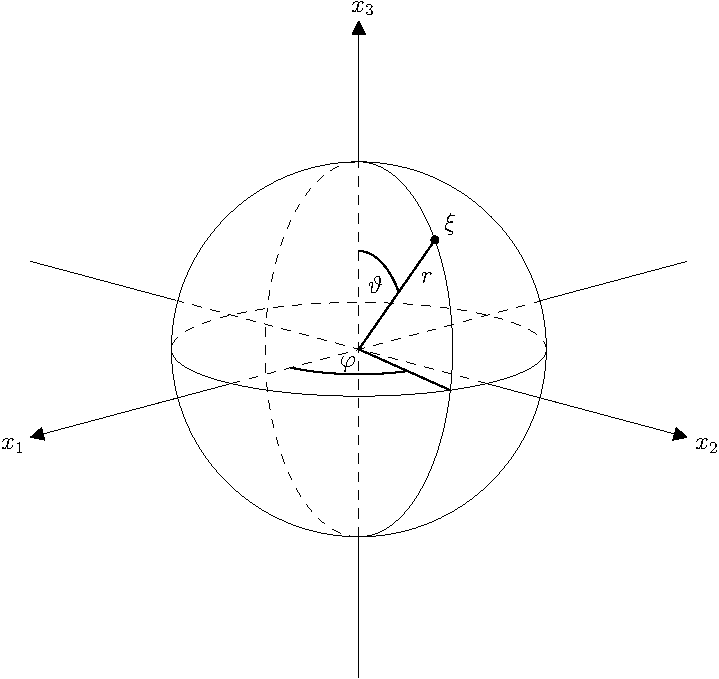
\includegraphics[width=0.45\textwidth]{sphere}}
\end{DoxyImageNoCaption}
 \end{center} 

For consistency with the other modules and the conventions used there, we also use {\itshape swapped} {\itshape scaled} {\itshape spherical} {\itshape coordinates} $x_1 := \frac{\varphi}{2\pi}$, $x_2 := \frac{\vartheta}{2\pi}$ and identify a point from $\mathbb{S}^2$ with the vector $\mathbf{x} := \left(x_1,x_2\right) \in [-\frac{1}{2}, \frac{1}{2}) \times [0,\frac{1}{2}]$.\hypertarget{group__nfsft_lp}{}\subsubsection{Legendre Polynomials}\label{group__nfsft_lp}
The {\itshape Legendre} {\itshape polynomials} $P_k : [-1,1] \rightarrow \mathbb{R}$, $k \in \mathbb{N}_{0}$ as {\itshape classical} {\itshape orthogonal} {\itshape polynomials} are given by their corresponding {\itshape Rodrigues} {\itshape formula} \[ P_k(t) := \frac{1}{2^k k!} \frac{\text{d}^k}{\text{d} t^k} \left(t^2-1\right)^k. \] The corresponding three-\/term recurrence relation is \[ (k+1)P_{k+1}(t) = (2k+1) x P_{k}(t) - k P_{k-1}(t) \quad (k \in \mathbb{N}_0). \] With \[ \left< f,g \right>_{\text{L}^2\left([-1,1]\right)} := \int_{-1}^{1} f(t) g(t) \text{d} t \] being the usual $\text{L}^2\left([-1,1]\right)$ inner product, the Legendre polynomials obey the orthogonality condition \[ \left< P_k,P_l \right>_{\text{L}^2\left([-1,1]\right)} = \frac{2}{2k+1} \delta_{k,l}. \]

\begin{DoxyRemark}{Remarks}
The normalisation constant $ c_k := \sqrt{\frac{2k+1}{2}}$ renders the scaled Legendre polynomials $c_k P_k$ orthonormal with respect to the induced $\text{L}^2\left([-1,1]\right)$ norm \[ \|f\|_{\text{L}^2\left([-1,1]\right)} := \left(<f,f>_{\text{L}^2\left([-1,1]\right)}\right)^{1/2} = \left(\int_{-1}^{1} |f(t)|^2 \; \text{d} t\right)^{1/2}. \]
\end{DoxyRemark}
\hypertarget{group__nfsft_alf}{}\subsubsection{Associated Legendre Functions}\label{group__nfsft_alf}
The {\itshape associated} {\itshape Legendre} {\itshape functions} $P_k^n : [-1,1] \rightarrow \mathbb{R} $, $n \in \mathbb{N}_0$, $k \ge n$ are defined by \[ P_k^n(t) := \left(\frac{(k-n)!}{(k+n)!}\right)^{1/2} \left(1-t^2\right)^{n/2} \frac{\text{d}^n}{\text{d} t^n} P_k(t). \] For $n = 0$, they coincide with the Legendre polynomials, i.\-e. $P_k^0 = P_k$. The associated Legendre functions obey the three-\/term recurrence relation \[ P_{k+1}^n(t) = v_{k}^n t P_k^n(t) + w_{k}^n P_{k-1}^n(t) \quad (k \ge n), \] with $P_{n-1}^n(t) := 0$, $P_{n}^n(t) := \frac{\sqrt{(2n)!}}{2^n n!} \left(1-t^2\right)^{n/2}$, and \[ v_{k}^n := \frac{2k+1}{((k-n+1)(k+n+1))^{1/2}}\; ,\qquad w_{k}^n := - \frac{((k-n)(k+n))^{1/2}}{((k-n+1)(k+n+1))^{1/2}}. \] For fixed $n$, the set $\left\{P_k^n:\: k \ge n\right\}$ forms a complete set of orthogonal functions in $\text{L}^2\left([-1,1]\right)$ with \[ \left< P_k^n,P_l^n \right>_{\text{L}^2\left([-1,1]\right)} = \frac{2}{2k+1} \delta_{k,l} \quad (0 \le n \le k,l). \]

\begin{DoxyRemark}{Remarks}
The normalisation constant $ c_k = \sqrt{\frac{2k+1}{2}}$ renders the scaled associated Legendre functions $c_k P_k^n$ orthonormal with respect to the induced $\text{L}^2\left([-1,1]\right)$ norm \[ \|f\|_{\text{L}^2\left([-1,1]\right)} := \left(<f,f>_{\text{L}^2\left([-1,1]\right)}\right)^{1/2} = \left(\int_{-1}^{1} |f(t)|^2 \; \text{d} t\right)^{1/2}. \]
\end{DoxyRemark}
\hypertarget{group__nfsft_sh}{}\subsubsection{Spherical Harmonics}\label{group__nfsft_sh}
The standard orthogonal basis of spherical harmonics for $\text{L}^2 \left(\mathbb{S}^2\right)$ with yet unnormalised basis functions $\tilde{Y}_k^n : \mathbb{S}^2 \rightarrow \mathbb{C}$ is given by \[ \tilde{Y}_k^n(\vartheta,\varphi) := P_k^{|n|}(\cos\vartheta) \mathrm{e}^{\mathrm{i} n \varphi} \] with the usual $\text{L}^2\left(\mathbb{S}^2\right)$ inner product \[ \left< f,g \right>_{\mathrm{L}^2\left(\mathbb{S}^2\right)} := \int_{\mathbb{S}^2} f(\vartheta,\varphi) \overline{g(\vartheta,\varphi)} \: \mathrm{d} \mathbf{\xi} := \int_{-\pi}^{\pi} \int_{0}^{\pi} f(\vartheta,\varphi) \overline{g(\vartheta,\varphi)} \sin \vartheta \; \mathrm{d} \vartheta \; \mathrm{d} \varphi. \] The normalisation constant $c_k^n := \sqrt{\frac{2k+1}{4\pi}}$ renders the scaled basis functions \[ Y_k^n(\vartheta,\varphi) := c_k^n P_k^{|n|}(\cos\vartheta) \mathrm{e}^{\mathrm{i} n \varphi} \] orthonormal with respect to the induced $\text{L}^2\left(\mathbb{S}^2 \right)$ norm \[ \|f\|_{\text{L}^2\left(\mathbb{S}^2\right)} = \left(<f,f>_{\text{L}^2\left(\mathbb{S}^2\right)}\right)^{1/2} = \left(\int_{-\pi}^{\pi} \int_{0}^{\pi} |f(\vartheta,\varphi)|^2 \sin \vartheta \; \mathrm{d} \vartheta \; \mathrm{d} \varphi\right)^{1/2}. \] A function $f \in \mathrm{L}^2\left(\mathbb{S}^2\right)$ has the orthogonal expansion \[ f = \sum_{k=0}^{\infty} \sum_{n=-k}^{k} \hat{f}(k,n) Y_k^n, \] where the coefficients $\hat{f}(k,n) := \left< f, Y_k^{n} \right>_{\mathrm{L}^2\left(\mathbb{S}^2\right)}$ are the {\itshape spherical} {\itshape Fourier} {\itshape coefficients} and the equivalence is understood in the $\mathrm{L}^2$-\/sense.\hypertarget{group__nfsft_nfsfts}{}\subsection{Nonuniform Fast Spherical Fourier Transforms}\label{group__nfsft_nfsfts}
This section describes the input and output relation of the spherical Fourier transform algorithms and the layout of the corresponding plan structure.\hypertarget{group__nfsft_ndsft}{}\subsubsection{Nonuniform Discrete Spherical Fourier Transform}\label{group__nfsft_ndsft}
The {\itshape nonuniform} {\itshape discrete} {\itshape spherical} {\itshape Fourier} {\itshape transform} ({\itshape N\-D\-S\-F\-T}) is defined as follows\-: \[ \begin{array}{rcl} \text{\textbf{Input}} & : & \text{coefficients } \hat{f}(k,n) \in \mathbb{C} \text{ for } k=0,\ldots,N,\;n=-k, \ldots,k,\; N \in \mathbb{N}_0,\\[1ex] & & \text{arbitrary nodes } \mathbf{x}(m) \in [-\frac{1}{2},\frac{1}{2}] \times [0,\frac{1}{2}] \text{ for } m=0,\ldots,M-1, M \in \mathbb{N}. \\[1ex] \text{\textbf{Task}} & : & \text{evaluate } f(m) := f\left( \mathbf{x}(m)\right) = \sum_{k=0}^N \sum_{n=-k}^k \hat{f}_k^n Y_k^n\left(\mathbf{x}(m)\right) \text{ for } m=0,\ldots,M-1. \\[1ex] \text{\textbf{Output}} & : & \text{coefficients } f(m) \in \mathbb{C} \text{ for } m=0,\ldots,M-1.\\ \end{array} \]\hypertarget{group__nfsft_andsft}{}\subsubsection{Adjoint Nonuniform Discrete Spherical Fourier Transform}\label{group__nfsft_andsft}
The {\itshape adjoint} {\itshape nonuniform} {\itshape discrete} {\itshape spherical} {\itshape Fourier} {\itshape transform} ({\itshape adjoint} {\itshape N\-D\-S\-F\-T}) is defined as follows\-: \[ \begin{array}{rcl} \text{\textbf{Input}} & : & \text{coefficients } f(m) \in \mathbb{C} \text{ for } m=0,\ldots,M-1, M \in \mathbb{N},\\ & & \text{arbitrary nodes } \mathbf{x}(m) \in [-\frac{1}{2},\frac{1}{2}] \times [0,\frac{1}{2}] \text{ for } m=0,\ldots,M-1, N \in \mathbb{N}_0.\\[1ex] \text{\textbf{Task}} & : & \text{evaluate } \hat{f}(k,n) := \sum_{m=0}^{M-1} f(m) \overline{Y_k^n\left(\mathbf{x}(m)\right)}cd Do \text{ for } k=0,\ldots,N,\;n=-k,\ldots,k.\\[1ex] \text{\textbf{Output}} & : & \text{coefficients } \hat{f}(k,n) \in \mathbb{C} \text{ for } k=0,\ldots,N,\;n=-k,\ldots,k.\\[1ex] \end{array} \]\hypertarget{group__nfsft_dl}{}\subsubsection{Data Layout}\label{group__nfsft_dl}
This section describes the public layout of the \hyperlink{structnfsft__plan}{nfsft\-\_\-plan} structure which contains all data for the computation of the aforementioned spherical Fourier transforms. The structure contains private (no read or write allowed), public read-\/only (only read access permitted), and public read-\/write (read and write access allowed) members. In the following, we indicate read and write access by {\ttfamily read} and {\ttfamily write}. The public members are structured as follows\-: \begin{DoxyItemize}
\item {\ttfamily N\-\_\-total} ({\ttfamily read}) The total number of components in {\ttfamily f\-\_\-hat}. If the bandwidth is $N \in \mathbb{N}_0$, the total number of components in {\ttfamily f\-\_\-hat} is {\ttfamily N\-\_\-total} $ = (2N+2)^2$. \item {\ttfamily M\-\_\-total} ({\ttfamily read}) the total number of samples $M$ \item {\ttfamily f\-\_\-hat} ({\ttfamily read-\/write}) The flattened array of spherical Fourier coefficents. The array has length $(2N+2)^2$ such that valid indices $i \in \mathbb{N}_0$ for array access {\ttfamily f\-\_\-hat} {\ttfamily }\mbox{[} $i$ {\ttfamily }\mbox{]} are $i=0,1,\ldots,(2N+2)^2-1$. However, only read and write access to indices corresponding to spherical Fourier coefficients $\hat{f}(k,n)$ is defined. The index $i$ corresponding to the spherical Fourier coefficient $\hat{f}(k,n)$ with $0 \le k \le M$, $-k \le n \le k$ is $i = (N+2)(N-n+1)+N+k+1$. For convenience, the helper macro \hyperlink{group__nfsft_ga8be22087991e0a82cfa59a3f0f2a5e86}{N\-F\-S\-F\-T\-\_\-\-I\-N\-D\-E\-X(k,n)} provides the necessary index calculations such that one can write {\ttfamily f\-\_\-hat}\mbox{[} {\ttfamily N\-F\-S\-F\-T\-\_\-\-I\-N\-D\-E\-X}( $k,n${\ttfamily })\mbox{]} {\ttfamily =} {\ttfamily }... to access the component corresponding to $\hat{f}(k,n)$. The data layout is due to implementation details. \item {\ttfamily f} ({\ttfamily read-\/write}) the array of coefficients $f(m)$ for $m=0,\ldots,M-1$ such that {\ttfamily f}\mbox{[} $m${\ttfamily }\mbox{]} = $f(m)$ \item {\ttfamily N} ({\ttfamily read}) the bandwidth $N \in \mathbb{N}_0$ \item {\ttfamily x} the array of nodes $\mathbf{x}(m) \in [-\frac{1}{2},\frac{1}{2}] \times [0,\frac{1}{2}]$ for $m = 0, \ldots,M-1$ such that {\ttfamily f}\mbox{[} $2m${\ttfamily }\mbox{]} = $x_1$ and {\ttfamily f}\mbox{[} $2m+1${\ttfamily }\mbox{]} = $x_2$\end{DoxyItemize}
\hypertarget{group__nfsft_gtn}{}\subsubsection{Good to know...}\label{group__nfsft_gtn}
When using the routines of this module you should bear in mind the following\-: \begin{DoxyItemize}
\item The bandwidth $N_{\text{max}}$ up to which precomputation is performed is always chosen as the next power of two with respect to the specified maximum bandwidth. \item By default, the N\-D\-S\-F\-T transforms (see nfsft\-\_\-direct\-\_\-trafo, \hyperlink{group__nfsft_ga5796fc68c432d46dfcab7abd8c56ee22}{nfsft\-\_\-trafo}) are allowed to destroy the input {\ttfamily f\-\_\-hat} while the input {\ttfamily x} is preserved. On the contrary, the adjoint N\-D\-S\-F\-T transforms (see nfsft\-\_\-direct\-\_\-adjoint, \hyperlink{group__nfsft_ga813bb48d404c7286310733c99a81a169}{nfsft\-\_\-adjoint}) do not destroy the input {\ttfamily f} and {\ttfamily x} by default. The desired behaviour can be assured by using the \hyperlink{group__nfsft_gac8a292845f0bdec6b0d8ef6eb693a00e}{N\-F\-S\-F\-T\-\_\-\-P\-R\-E\-S\-E\-R\-V\-E\-\_\-\-F\-\_\-\-H\-A\-T}, \hyperlink{group__nfsft_gacf7d73753b74dbf148167c3d46226f09}{N\-F\-S\-F\-T\-\_\-\-P\-R\-E\-S\-E\-R\-V\-E\-\_\-\-X}, \hyperlink{group__nfsft_ga45962e763c2c551c1ea764a68b686b5c}{N\-F\-S\-F\-T\-\_\-\-P\-R\-E\-S\-E\-R\-V\-E\-\_\-\-F} and \hyperlink{group__nfsft_gaa808899fc4db422c7b23470e6baad904}{N\-F\-S\-F\-T\-\_\-\-D\-E\-S\-T\-R\-O\-Y\-\_\-\-F\-\_\-\-H\-A\-T}, \hyperlink{group__nfsft_ga6f22df0b292db920d795b3e3569181f2}{N\-F\-S\-F\-T\-\_\-\-D\-E\-S\-T\-R\-O\-Y\-\_\-\-X}, \hyperlink{group__nfsft_ga2b32e2eabd33bf0886f6df45365d04c0}{N\-F\-S\-F\-T\-\_\-\-D\-E\-S\-T\-R\-O\-Y\-\_\-\-F} flags. \end{DoxyItemize}


\subsection{Macro Definition Documentation}
\hypertarget{group__nfsft_ga65036f479a7421863956c02aa78bc9be}{\index{N\-F\-S\-F\-T -\/ Nonequispaced fast spherical Fourier transform@{N\-F\-S\-F\-T -\/ Nonequispaced fast spherical Fourier transform}!N\-F\-S\-F\-T\-\_\-\-N\-O\-R\-M\-A\-L\-I\-Z\-E\-D@{N\-F\-S\-F\-T\-\_\-\-N\-O\-R\-M\-A\-L\-I\-Z\-E\-D}}
\index{N\-F\-S\-F\-T\-\_\-\-N\-O\-R\-M\-A\-L\-I\-Z\-E\-D@{N\-F\-S\-F\-T\-\_\-\-N\-O\-R\-M\-A\-L\-I\-Z\-E\-D}!NFSFT - Nonequispaced fast spherical Fourier transform@{N\-F\-S\-F\-T -\/ Nonequispaced fast spherical Fourier transform}}
\subsubsection[{N\-F\-S\-F\-T\-\_\-\-N\-O\-R\-M\-A\-L\-I\-Z\-E\-D}]{\setlength{\rightskip}{0pt plus 5cm}\#define N\-F\-S\-F\-T\-\_\-\-N\-O\-R\-M\-A\-L\-I\-Z\-E\-D~(1\-U $<$$<$ 0)}}\label{group__nfsft_ga65036f479a7421863956c02aa78bc9be}
By default, all computations are performed with respect to the unnormalized basis functions \[ \tilde{Y}_k^n(\vartheta,\varphi) = P_k^{|n|}(\cos\vartheta) \mathrm{e}^{\mathrm{i} n \varphi}. \] If this flag is set, all computations are carried out using the $L_2$-\/ normalized basis functions \[ Y_k^n(\vartheta,\varphi) = \sqrt{\frac{2k+1}{4\pi}} P_k^{|n|}(\cos\vartheta) \mathrm{e}^{\mathrm{i} n \varphi}. \]

\begin{DoxySeeAlso}{See Also}
\hyperlink{group__nfsft_ga65cda3f4a3edc5eb39c697cf34b1f0b9}{nfsft\-\_\-init} 

\hyperlink{group__nfsft_ga2812aa5beba0eb7efd3072bf323a0155}{nfsft\-\_\-init\-\_\-advanced} 

nfsft\-\_\-init\-\_\-guru 
\end{DoxySeeAlso}
\begin{DoxyAuthor}{Author}
Jens Keiner 
\end{DoxyAuthor}


Definition at line 575 of file nfft3.\-h.



Referenced by main(), nfsft\-\_\-adjoint(), and nfsft\-\_\-trafo().

\hypertarget{group__nfsft_gaba029560a4a506c8f2dad185511db827}{\index{N\-F\-S\-F\-T -\/ Nonequispaced fast spherical Fourier transform@{N\-F\-S\-F\-T -\/ Nonequispaced fast spherical Fourier transform}!N\-F\-S\-F\-T\-\_\-\-U\-S\-E\-\_\-\-N\-D\-F\-T@{N\-F\-S\-F\-T\-\_\-\-U\-S\-E\-\_\-\-N\-D\-F\-T}}
\index{N\-F\-S\-F\-T\-\_\-\-U\-S\-E\-\_\-\-N\-D\-F\-T@{N\-F\-S\-F\-T\-\_\-\-U\-S\-E\-\_\-\-N\-D\-F\-T}!NFSFT - Nonequispaced fast spherical Fourier transform@{N\-F\-S\-F\-T -\/ Nonequispaced fast spherical Fourier transform}}
\subsubsection[{N\-F\-S\-F\-T\-\_\-\-U\-S\-E\-\_\-\-N\-D\-F\-T}]{\setlength{\rightskip}{0pt plus 5cm}\#define N\-F\-S\-F\-T\-\_\-\-U\-S\-E\-\_\-\-N\-D\-F\-T~(1\-U $<$$<$ 1)}}\label{group__nfsft_gaba029560a4a506c8f2dad185511db827}
If this flag is set, the fast N\-F\-S\-F\-T algorithms (see \hyperlink{group__nfsft_ga5796fc68c432d46dfcab7abd8c56ee22}{nfsft\-\_\-trafo}, \hyperlink{group__nfsft_ga813bb48d404c7286310733c99a81a169}{nfsft\-\_\-adjoint}) will use internally the exact but usually slower direct N\-D\-F\-T algorithm in favor of fast but approximative N\-F\-F\-T algorithm.

\begin{DoxySeeAlso}{See Also}
\hyperlink{group__nfsft_ga65cda3f4a3edc5eb39c697cf34b1f0b9}{nfsft\-\_\-init} 

\hyperlink{group__nfsft_ga2812aa5beba0eb7efd3072bf323a0155}{nfsft\-\_\-init\-\_\-advanced} 

nfsft\-\_\-init\-\_\-guru 
\end{DoxySeeAlso}
\begin{DoxyAuthor}{Author}
Jens Keiner 
\end{DoxyAuthor}


Definition at line 576 of file nfft3.\-h.



Referenced by main(), nfsft\-\_\-adjoint(), and nfsft\-\_\-trafo().

\hypertarget{group__nfsft_ga6b9eed1e7bcf862dcc3111509075fcbb}{\index{N\-F\-S\-F\-T -\/ Nonequispaced fast spherical Fourier transform@{N\-F\-S\-F\-T -\/ Nonequispaced fast spherical Fourier transform}!N\-F\-S\-F\-T\-\_\-\-U\-S\-E\-\_\-\-D\-P\-T@{N\-F\-S\-F\-T\-\_\-\-U\-S\-E\-\_\-\-D\-P\-T}}
\index{N\-F\-S\-F\-T\-\_\-\-U\-S\-E\-\_\-\-D\-P\-T@{N\-F\-S\-F\-T\-\_\-\-U\-S\-E\-\_\-\-D\-P\-T}!NFSFT - Nonequispaced fast spherical Fourier transform@{N\-F\-S\-F\-T -\/ Nonequispaced fast spherical Fourier transform}}
\subsubsection[{N\-F\-S\-F\-T\-\_\-\-U\-S\-E\-\_\-\-D\-P\-T}]{\setlength{\rightskip}{0pt plus 5cm}\#define N\-F\-S\-F\-T\-\_\-\-U\-S\-E\-\_\-\-D\-P\-T~(1\-U $<$$<$ 2)}}\label{group__nfsft_ga6b9eed1e7bcf862dcc3111509075fcbb}
If this flag is set, the fast N\-F\-S\-F\-T algorithms (see \hyperlink{group__nfsft_ga5796fc68c432d46dfcab7abd8c56ee22}{nfsft\-\_\-trafo}, \hyperlink{group__nfsft_ga813bb48d404c7286310733c99a81a169}{nfsft\-\_\-adjoint}) will use internally the usually slower direct D\-P\-T algorithm in favor of the fast F\-P\-T algorithm.

\begin{DoxySeeAlso}{See Also}
\hyperlink{group__nfsft_ga65cda3f4a3edc5eb39c697cf34b1f0b9}{nfsft\-\_\-init} 

\hyperlink{group__nfsft_ga2812aa5beba0eb7efd3072bf323a0155}{nfsft\-\_\-init\-\_\-advanced} 

nfsft\-\_\-init\-\_\-guru 
\end{DoxySeeAlso}
\begin{DoxyAuthor}{Author}
Jens Keiner 
\end{DoxyAuthor}
\begin{DoxyWarning}{Warning}
This feature is not implemented yet! 
\end{DoxyWarning}


Definition at line 577 of file nfft3.\-h.



Referenced by main(), nfsft\-\_\-adjoint(), and nfsft\-\_\-trafo().

\hypertarget{group__nfsft_ga02e4313d15b24c79e6802f853d452454}{\index{N\-F\-S\-F\-T -\/ Nonequispaced fast spherical Fourier transform@{N\-F\-S\-F\-T -\/ Nonequispaced fast spherical Fourier transform}!N\-F\-S\-F\-T\-\_\-\-M\-A\-L\-L\-O\-C\-\_\-\-X@{N\-F\-S\-F\-T\-\_\-\-M\-A\-L\-L\-O\-C\-\_\-\-X}}
\index{N\-F\-S\-F\-T\-\_\-\-M\-A\-L\-L\-O\-C\-\_\-\-X@{N\-F\-S\-F\-T\-\_\-\-M\-A\-L\-L\-O\-C\-\_\-\-X}!NFSFT - Nonequispaced fast spherical Fourier transform@{N\-F\-S\-F\-T -\/ Nonequispaced fast spherical Fourier transform}}
\subsubsection[{N\-F\-S\-F\-T\-\_\-\-M\-A\-L\-L\-O\-C\-\_\-\-X}]{\setlength{\rightskip}{0pt plus 5cm}\#define N\-F\-S\-F\-T\-\_\-\-M\-A\-L\-L\-O\-C\-\_\-\-X~(1\-U $<$$<$ 3)}}\label{group__nfsft_ga02e4313d15b24c79e6802f853d452454}
If this flag is set, the init methods (see \hyperlink{group__nfsft_ga65cda3f4a3edc5eb39c697cf34b1f0b9}{nfsft\-\_\-init} , \hyperlink{group__nfsft_ga2812aa5beba0eb7efd3072bf323a0155}{nfsft\-\_\-init\-\_\-advanced} , and nfsft\-\_\-init\-\_\-guru) will allocate memory and the method \hyperlink{group__nfsft_gaa63e193a27d84059742ff25ff81e2ed1}{nfsft\-\_\-finalize} will free the array {\ttfamily x} for you. Otherwise, you have to assure by yourself that {\ttfamily x} points to an array of proper size before excuting a transform and you are responsible for freeing the corresponding memory before program termination.

\begin{DoxySeeAlso}{See Also}
\hyperlink{group__nfsft_ga65cda3f4a3edc5eb39c697cf34b1f0b9}{nfsft\-\_\-init} 

\hyperlink{group__nfsft_ga2812aa5beba0eb7efd3072bf323a0155}{nfsft\-\_\-init\-\_\-advanced} 

nfsft\-\_\-init\-\_\-guru 
\end{DoxySeeAlso}
\begin{DoxyAuthor}{Author}
Jens Keiner 
\end{DoxyAuthor}


Definition at line 578 of file nfft3.\-h.



Referenced by main(), nfsft\-\_\-finalize(), and nfsft\-\_\-init().

\hypertarget{group__nfsft_gab76dcf8db948f18cc87403dac804fc68}{\index{N\-F\-S\-F\-T -\/ Nonequispaced fast spherical Fourier transform@{N\-F\-S\-F\-T -\/ Nonequispaced fast spherical Fourier transform}!N\-F\-S\-F\-T\-\_\-\-M\-A\-L\-L\-O\-C\-\_\-\-F\-\_\-\-H\-A\-T@{N\-F\-S\-F\-T\-\_\-\-M\-A\-L\-L\-O\-C\-\_\-\-F\-\_\-\-H\-A\-T}}
\index{N\-F\-S\-F\-T\-\_\-\-M\-A\-L\-L\-O\-C\-\_\-\-F\-\_\-\-H\-A\-T@{N\-F\-S\-F\-T\-\_\-\-M\-A\-L\-L\-O\-C\-\_\-\-F\-\_\-\-H\-A\-T}!NFSFT - Nonequispaced fast spherical Fourier transform@{N\-F\-S\-F\-T -\/ Nonequispaced fast spherical Fourier transform}}
\subsubsection[{N\-F\-S\-F\-T\-\_\-\-M\-A\-L\-L\-O\-C\-\_\-\-F\-\_\-\-H\-A\-T}]{\setlength{\rightskip}{0pt plus 5cm}\#define N\-F\-S\-F\-T\-\_\-\-M\-A\-L\-L\-O\-C\-\_\-\-F\-\_\-\-H\-A\-T~(1\-U $<$$<$ 5)}}\label{group__nfsft_gab76dcf8db948f18cc87403dac804fc68}
If this flag is set, the init methods (see \hyperlink{group__nfsft_ga65cda3f4a3edc5eb39c697cf34b1f0b9}{nfsft\-\_\-init} , \hyperlink{group__nfsft_ga2812aa5beba0eb7efd3072bf323a0155}{nfsft\-\_\-init\-\_\-advanced} , and nfsft\-\_\-init\-\_\-guru) will allocate memory and the method \hyperlink{group__nfsft_gaa63e193a27d84059742ff25ff81e2ed1}{nfsft\-\_\-finalize} will free the array {\ttfamily f\-\_\-hat} for you. Otherwise, you have to assure by yourself that {\ttfamily f\-\_\-hat} points to an array of proper size before excuting a transform and you are responsible for freeing the corresponding memory before program termination.

\begin{DoxySeeAlso}{See Also}
\hyperlink{group__nfsft_ga65cda3f4a3edc5eb39c697cf34b1f0b9}{nfsft\-\_\-init} 

\hyperlink{group__nfsft_ga2812aa5beba0eb7efd3072bf323a0155}{nfsft\-\_\-init\-\_\-advanced} 

nfsft\-\_\-init\-\_\-guru 
\end{DoxySeeAlso}
\begin{DoxyAuthor}{Author}
Jens Keiner 
\end{DoxyAuthor}


Definition at line 579 of file nfft3.\-h.



Referenced by main(), nfsft\-\_\-finalize(), and nfsft\-\_\-init().

\hypertarget{group__nfsft_gaf3bc3ab774cda0c1c765e97066893d30}{\index{N\-F\-S\-F\-T -\/ Nonequispaced fast spherical Fourier transform@{N\-F\-S\-F\-T -\/ Nonequispaced fast spherical Fourier transform}!N\-F\-S\-F\-T\-\_\-\-M\-A\-L\-L\-O\-C\-\_\-\-F@{N\-F\-S\-F\-T\-\_\-\-M\-A\-L\-L\-O\-C\-\_\-\-F}}
\index{N\-F\-S\-F\-T\-\_\-\-M\-A\-L\-L\-O\-C\-\_\-\-F@{N\-F\-S\-F\-T\-\_\-\-M\-A\-L\-L\-O\-C\-\_\-\-F}!NFSFT - Nonequispaced fast spherical Fourier transform@{N\-F\-S\-F\-T -\/ Nonequispaced fast spherical Fourier transform}}
\subsubsection[{N\-F\-S\-F\-T\-\_\-\-M\-A\-L\-L\-O\-C\-\_\-\-F}]{\setlength{\rightskip}{0pt plus 5cm}\#define N\-F\-S\-F\-T\-\_\-\-M\-A\-L\-L\-O\-C\-\_\-\-F~(1\-U $<$$<$ 6)}}\label{group__nfsft_gaf3bc3ab774cda0c1c765e97066893d30}
If this flag is set, the init methods (see \hyperlink{group__nfsft_ga65cda3f4a3edc5eb39c697cf34b1f0b9}{nfsft\-\_\-init} , \hyperlink{group__nfsft_ga2812aa5beba0eb7efd3072bf323a0155}{nfsft\-\_\-init\-\_\-advanced} , and nfsft\-\_\-init\-\_\-guru) will allocate memory and the method \hyperlink{group__nfsft_gaa63e193a27d84059742ff25ff81e2ed1}{nfsft\-\_\-finalize} will free the array {\ttfamily f} for you. Otherwise, you have to assure by yourself that {\ttfamily f} points to an array of proper size before excuting a transform and you are responsible for freeing the corresponding memory before program termination.

\begin{DoxySeeAlso}{See Also}
\hyperlink{group__nfsft_ga65cda3f4a3edc5eb39c697cf34b1f0b9}{nfsft\-\_\-init} 

\hyperlink{group__nfsft_ga2812aa5beba0eb7efd3072bf323a0155}{nfsft\-\_\-init\-\_\-advanced} 

nfsft\-\_\-init\-\_\-guru 
\end{DoxySeeAlso}
\begin{DoxyAuthor}{Author}
Jens Keiner 
\end{DoxyAuthor}


Definition at line 580 of file nfft3.\-h.



Referenced by main(), nfsft\-\_\-finalize(), and nfsft\-\_\-init().

\hypertarget{group__nfsft_gac8a292845f0bdec6b0d8ef6eb693a00e}{\index{N\-F\-S\-F\-T -\/ Nonequispaced fast spherical Fourier transform@{N\-F\-S\-F\-T -\/ Nonequispaced fast spherical Fourier transform}!N\-F\-S\-F\-T\-\_\-\-P\-R\-E\-S\-E\-R\-V\-E\-\_\-\-F\-\_\-\-H\-A\-T@{N\-F\-S\-F\-T\-\_\-\-P\-R\-E\-S\-E\-R\-V\-E\-\_\-\-F\-\_\-\-H\-A\-T}}
\index{N\-F\-S\-F\-T\-\_\-\-P\-R\-E\-S\-E\-R\-V\-E\-\_\-\-F\-\_\-\-H\-A\-T@{N\-F\-S\-F\-T\-\_\-\-P\-R\-E\-S\-E\-R\-V\-E\-\_\-\-F\-\_\-\-H\-A\-T}!NFSFT - Nonequispaced fast spherical Fourier transform@{N\-F\-S\-F\-T -\/ Nonequispaced fast spherical Fourier transform}}
\subsubsection[{N\-F\-S\-F\-T\-\_\-\-P\-R\-E\-S\-E\-R\-V\-E\-\_\-\-F\-\_\-\-H\-A\-T}]{\setlength{\rightskip}{0pt plus 5cm}\#define N\-F\-S\-F\-T\-\_\-\-P\-R\-E\-S\-E\-R\-V\-E\-\_\-\-F\-\_\-\-H\-A\-T~(1\-U $<$$<$ 7)}}\label{group__nfsft_gac8a292845f0bdec6b0d8ef6eb693a00e}
If this flag is set, it is guaranteed that during an execution of nfsft\-\_\-direct\-\_\-trafo or \hyperlink{group__nfsft_ga5796fc68c432d46dfcab7abd8c56ee22}{nfsft\-\_\-trafo} the content of {\ttfamily f\-\_\-hat} remains unchanged.

\begin{DoxySeeAlso}{See Also}
\hyperlink{group__nfsft_ga65cda3f4a3edc5eb39c697cf34b1f0b9}{nfsft\-\_\-init} 

\hyperlink{group__nfsft_ga2812aa5beba0eb7efd3072bf323a0155}{nfsft\-\_\-init\-\_\-advanced} 

nfsft\-\_\-init\-\_\-guru 
\end{DoxySeeAlso}
\begin{DoxyAuthor}{Author}
Jens Keiner 
\end{DoxyAuthor}


Definition at line 581 of file nfft3.\-h.



Referenced by nfsft\-\_\-finalize(), and nfsft\-\_\-trafo().

\hypertarget{group__nfsft_gacf7d73753b74dbf148167c3d46226f09}{\index{N\-F\-S\-F\-T -\/ Nonequispaced fast spherical Fourier transform@{N\-F\-S\-F\-T -\/ Nonequispaced fast spherical Fourier transform}!N\-F\-S\-F\-T\-\_\-\-P\-R\-E\-S\-E\-R\-V\-E\-\_\-\-X@{N\-F\-S\-F\-T\-\_\-\-P\-R\-E\-S\-E\-R\-V\-E\-\_\-\-X}}
\index{N\-F\-S\-F\-T\-\_\-\-P\-R\-E\-S\-E\-R\-V\-E\-\_\-\-X@{N\-F\-S\-F\-T\-\_\-\-P\-R\-E\-S\-E\-R\-V\-E\-\_\-\-X}!NFSFT - Nonequispaced fast spherical Fourier transform@{N\-F\-S\-F\-T -\/ Nonequispaced fast spherical Fourier transform}}
\subsubsection[{N\-F\-S\-F\-T\-\_\-\-P\-R\-E\-S\-E\-R\-V\-E\-\_\-\-X}]{\setlength{\rightskip}{0pt plus 5cm}\#define N\-F\-S\-F\-T\-\_\-\-P\-R\-E\-S\-E\-R\-V\-E\-\_\-\-X~(1\-U $<$$<$ 8)}}\label{group__nfsft_gacf7d73753b74dbf148167c3d46226f09}
If this flag is set, it is guaranteed that during an execution of nfsft\-\_\-direct\-\_\-trafo, \hyperlink{group__nfsft_ga5796fc68c432d46dfcab7abd8c56ee22}{nfsft\-\_\-trafo} or nfsft\-\_\-direct\-\_\-adjoint, \hyperlink{group__nfsft_ga813bb48d404c7286310733c99a81a169}{nfsft\-\_\-adjoint} the content of {\ttfamily x} remains unchanged.

\begin{DoxySeeAlso}{See Also}
\hyperlink{group__nfsft_ga65cda3f4a3edc5eb39c697cf34b1f0b9}{nfsft\-\_\-init} 

\hyperlink{group__nfsft_ga2812aa5beba0eb7efd3072bf323a0155}{nfsft\-\_\-init\-\_\-advanced} 

nfsft\-\_\-init\-\_\-guru 
\end{DoxySeeAlso}
\begin{DoxyAuthor}{Author}
Jens Keiner 
\end{DoxyAuthor}


Definition at line 582 of file nfft3.\-h.

\hypertarget{group__nfsft_ga45962e763c2c551c1ea764a68b686b5c}{\index{N\-F\-S\-F\-T -\/ Nonequispaced fast spherical Fourier transform@{N\-F\-S\-F\-T -\/ Nonequispaced fast spherical Fourier transform}!N\-F\-S\-F\-T\-\_\-\-P\-R\-E\-S\-E\-R\-V\-E\-\_\-\-F@{N\-F\-S\-F\-T\-\_\-\-P\-R\-E\-S\-E\-R\-V\-E\-\_\-\-F}}
\index{N\-F\-S\-F\-T\-\_\-\-P\-R\-E\-S\-E\-R\-V\-E\-\_\-\-F@{N\-F\-S\-F\-T\-\_\-\-P\-R\-E\-S\-E\-R\-V\-E\-\_\-\-F}!NFSFT - Nonequispaced fast spherical Fourier transform@{N\-F\-S\-F\-T -\/ Nonequispaced fast spherical Fourier transform}}
\subsubsection[{N\-F\-S\-F\-T\-\_\-\-P\-R\-E\-S\-E\-R\-V\-E\-\_\-\-F}]{\setlength{\rightskip}{0pt plus 5cm}\#define N\-F\-S\-F\-T\-\_\-\-P\-R\-E\-S\-E\-R\-V\-E\-\_\-\-F~(1\-U $<$$<$ 9)}}\label{group__nfsft_ga45962e763c2c551c1ea764a68b686b5c}
If this flag is set, it is guaranteed that during an execution of nfsft\-\_\-direct\-\_\-adjoint or \hyperlink{group__nfsft_ga813bb48d404c7286310733c99a81a169}{nfsft\-\_\-adjoint} the content of {\ttfamily f} remains unchanged.

\begin{DoxySeeAlso}{See Also}
\hyperlink{group__nfsft_ga65cda3f4a3edc5eb39c697cf34b1f0b9}{nfsft\-\_\-init} 

\hyperlink{group__nfsft_ga2812aa5beba0eb7efd3072bf323a0155}{nfsft\-\_\-init\-\_\-advanced} 

nfsft\-\_\-init\-\_\-guru 
\end{DoxySeeAlso}
\begin{DoxyAuthor}{Author}
Jens Keiner 
\end{DoxyAuthor}


Definition at line 583 of file nfft3.\-h.

\hypertarget{group__nfsft_gaa808899fc4db422c7b23470e6baad904}{\index{N\-F\-S\-F\-T -\/ Nonequispaced fast spherical Fourier transform@{N\-F\-S\-F\-T -\/ Nonequispaced fast spherical Fourier transform}!N\-F\-S\-F\-T\-\_\-\-D\-E\-S\-T\-R\-O\-Y\-\_\-\-F\-\_\-\-H\-A\-T@{N\-F\-S\-F\-T\-\_\-\-D\-E\-S\-T\-R\-O\-Y\-\_\-\-F\-\_\-\-H\-A\-T}}
\index{N\-F\-S\-F\-T\-\_\-\-D\-E\-S\-T\-R\-O\-Y\-\_\-\-F\-\_\-\-H\-A\-T@{N\-F\-S\-F\-T\-\_\-\-D\-E\-S\-T\-R\-O\-Y\-\_\-\-F\-\_\-\-H\-A\-T}!NFSFT - Nonequispaced fast spherical Fourier transform@{N\-F\-S\-F\-T -\/ Nonequispaced fast spherical Fourier transform}}
\subsubsection[{N\-F\-S\-F\-T\-\_\-\-D\-E\-S\-T\-R\-O\-Y\-\_\-\-F\-\_\-\-H\-A\-T}]{\setlength{\rightskip}{0pt plus 5cm}\#define N\-F\-S\-F\-T\-\_\-\-D\-E\-S\-T\-R\-O\-Y\-\_\-\-F\-\_\-\-H\-A\-T~(1\-U $<$$<$ 10)}}\label{group__nfsft_gaa808899fc4db422c7b23470e6baad904}
If this flag is set, it is explicitely allowed that during an execution of nfsft\-\_\-direct\-\_\-trafo or \hyperlink{group__nfsft_ga5796fc68c432d46dfcab7abd8c56ee22}{nfsft\-\_\-trafo} the content of {\ttfamily f\-\_\-hat} may be changed.

\begin{DoxySeeAlso}{See Also}
\hyperlink{group__nfsft_ga65cda3f4a3edc5eb39c697cf34b1f0b9}{nfsft\-\_\-init} 

\hyperlink{group__nfsft_ga2812aa5beba0eb7efd3072bf323a0155}{nfsft\-\_\-init\-\_\-advanced} 

nfsft\-\_\-init\-\_\-guru 
\end{DoxySeeAlso}
\begin{DoxyAuthor}{Author}
Jens Keiner 
\end{DoxyAuthor}


Definition at line 584 of file nfft3.\-h.

\hypertarget{group__nfsft_ga6f22df0b292db920d795b3e3569181f2}{\index{N\-F\-S\-F\-T -\/ Nonequispaced fast spherical Fourier transform@{N\-F\-S\-F\-T -\/ Nonequispaced fast spherical Fourier transform}!N\-F\-S\-F\-T\-\_\-\-D\-E\-S\-T\-R\-O\-Y\-\_\-\-X@{N\-F\-S\-F\-T\-\_\-\-D\-E\-S\-T\-R\-O\-Y\-\_\-\-X}}
\index{N\-F\-S\-F\-T\-\_\-\-D\-E\-S\-T\-R\-O\-Y\-\_\-\-X@{N\-F\-S\-F\-T\-\_\-\-D\-E\-S\-T\-R\-O\-Y\-\_\-\-X}!NFSFT - Nonequispaced fast spherical Fourier transform@{N\-F\-S\-F\-T -\/ Nonequispaced fast spherical Fourier transform}}
\subsubsection[{N\-F\-S\-F\-T\-\_\-\-D\-E\-S\-T\-R\-O\-Y\-\_\-\-X}]{\setlength{\rightskip}{0pt plus 5cm}\#define N\-F\-S\-F\-T\-\_\-\-D\-E\-S\-T\-R\-O\-Y\-\_\-\-X~(1\-U $<$$<$ 11)}}\label{group__nfsft_ga6f22df0b292db920d795b3e3569181f2}
If this flag is set, it is explicitely allowed that during an execution of nfsft\-\_\-direct\-\_\-trafo, \hyperlink{group__nfsft_ga5796fc68c432d46dfcab7abd8c56ee22}{nfsft\-\_\-trafo} or nfsft\-\_\-direct\-\_\-adjoint, \hyperlink{group__nfsft_ga813bb48d404c7286310733c99a81a169}{nfsft\-\_\-adjoint} the content of {\ttfamily x} may be changed.

\begin{DoxySeeAlso}{See Also}
\hyperlink{group__nfsft_ga65cda3f4a3edc5eb39c697cf34b1f0b9}{nfsft\-\_\-init} 

\hyperlink{group__nfsft_ga2812aa5beba0eb7efd3072bf323a0155}{nfsft\-\_\-init\-\_\-advanced} 

nfsft\-\_\-init\-\_\-guru 
\end{DoxySeeAlso}
\begin{DoxyAuthor}{Author}
Jens Keiner 
\end{DoxyAuthor}


Definition at line 585 of file nfft3.\-h.

\hypertarget{group__nfsft_ga2b32e2eabd33bf0886f6df45365d04c0}{\index{N\-F\-S\-F\-T -\/ Nonequispaced fast spherical Fourier transform@{N\-F\-S\-F\-T -\/ Nonequispaced fast spherical Fourier transform}!N\-F\-S\-F\-T\-\_\-\-D\-E\-S\-T\-R\-O\-Y\-\_\-\-F@{N\-F\-S\-F\-T\-\_\-\-D\-E\-S\-T\-R\-O\-Y\-\_\-\-F}}
\index{N\-F\-S\-F\-T\-\_\-\-D\-E\-S\-T\-R\-O\-Y\-\_\-\-F@{N\-F\-S\-F\-T\-\_\-\-D\-E\-S\-T\-R\-O\-Y\-\_\-\-F}!NFSFT - Nonequispaced fast spherical Fourier transform@{N\-F\-S\-F\-T -\/ Nonequispaced fast spherical Fourier transform}}
\subsubsection[{N\-F\-S\-F\-T\-\_\-\-D\-E\-S\-T\-R\-O\-Y\-\_\-\-F}]{\setlength{\rightskip}{0pt plus 5cm}\#define N\-F\-S\-F\-T\-\_\-\-D\-E\-S\-T\-R\-O\-Y\-\_\-\-F~(1\-U $<$$<$ 12)}}\label{group__nfsft_ga2b32e2eabd33bf0886f6df45365d04c0}
If this flag is set, it is explicitely allowed that during an execution of nfsft\-\_\-direct\-\_\-adjoint or \hyperlink{group__nfsft_ga813bb48d404c7286310733c99a81a169}{nfsft\-\_\-adjoint} the content of {\ttfamily f} may be changed.

\begin{DoxySeeAlso}{See Also}
\hyperlink{group__nfsft_ga65cda3f4a3edc5eb39c697cf34b1f0b9}{nfsft\-\_\-init} 

\hyperlink{group__nfsft_ga2812aa5beba0eb7efd3072bf323a0155}{nfsft\-\_\-init\-\_\-advanced} 

nfsft\-\_\-init\-\_\-guru 
\end{DoxySeeAlso}
\begin{DoxyAuthor}{Author}
Jens Keiner 
\end{DoxyAuthor}


Definition at line 586 of file nfft3.\-h.

\hypertarget{group__nfsft_ga9ed987164acf6e362ab2878506fbca95}{\index{N\-F\-S\-F\-T -\/ Nonequispaced fast spherical Fourier transform@{N\-F\-S\-F\-T -\/ Nonequispaced fast spherical Fourier transform}!N\-F\-S\-F\-T\-\_\-\-N\-O\-\_\-\-D\-I\-R\-E\-C\-T\-\_\-\-A\-L\-G\-O\-R\-I\-T\-H\-M@{N\-F\-S\-F\-T\-\_\-\-N\-O\-\_\-\-D\-I\-R\-E\-C\-T\-\_\-\-A\-L\-G\-O\-R\-I\-T\-H\-M}}
\index{N\-F\-S\-F\-T\-\_\-\-N\-O\-\_\-\-D\-I\-R\-E\-C\-T\-\_\-\-A\-L\-G\-O\-R\-I\-T\-H\-M@{N\-F\-S\-F\-T\-\_\-\-N\-O\-\_\-\-D\-I\-R\-E\-C\-T\-\_\-\-A\-L\-G\-O\-R\-I\-T\-H\-M}!NFSFT - Nonequispaced fast spherical Fourier transform@{N\-F\-S\-F\-T -\/ Nonequispaced fast spherical Fourier transform}}
\subsubsection[{N\-F\-S\-F\-T\-\_\-\-N\-O\-\_\-\-D\-I\-R\-E\-C\-T\-\_\-\-A\-L\-G\-O\-R\-I\-T\-H\-M}]{\setlength{\rightskip}{0pt plus 5cm}\#define N\-F\-S\-F\-T\-\_\-\-N\-O\-\_\-\-D\-I\-R\-E\-C\-T\-\_\-\-A\-L\-G\-O\-R\-I\-T\-H\-M~(1\-U $<$$<$ 13)}}\label{group__nfsft_ga9ed987164acf6e362ab2878506fbca95}
If this flag is set, the transforms nfsft\-\_\-direct\-\_\-trafo and nfsft\-\_\-direct\-\_\-adjoint do not work. Setting this flag saves some memory for precomputed data.

\begin{DoxySeeAlso}{See Also}
\hyperlink{group__nfsft_gabe87aeea1f7cfef9ae8febb16d702f3b}{nfsft\-\_\-precompute} 

nfsft\-\_\-direct\-\_\-trafo 

nfsft\-\_\-direct\-\_\-adjoint 
\end{DoxySeeAlso}
\begin{DoxyAuthor}{Author}
Jens Keiner 
\end{DoxyAuthor}


Definition at line 589 of file nfft3.\-h.



Referenced by nfsft\-\_\-forget(), and nfsft\-\_\-precompute().

\hypertarget{group__nfsft_gaa228bbed7ddbbb4a15f1cd11ec27b415}{\index{N\-F\-S\-F\-T -\/ Nonequispaced fast spherical Fourier transform@{N\-F\-S\-F\-T -\/ Nonequispaced fast spherical Fourier transform}!N\-F\-S\-F\-T\-\_\-\-N\-O\-\_\-\-F\-A\-S\-T\-\_\-\-A\-L\-G\-O\-R\-I\-T\-H\-M@{N\-F\-S\-F\-T\-\_\-\-N\-O\-\_\-\-F\-A\-S\-T\-\_\-\-A\-L\-G\-O\-R\-I\-T\-H\-M}}
\index{N\-F\-S\-F\-T\-\_\-\-N\-O\-\_\-\-F\-A\-S\-T\-\_\-\-A\-L\-G\-O\-R\-I\-T\-H\-M@{N\-F\-S\-F\-T\-\_\-\-N\-O\-\_\-\-F\-A\-S\-T\-\_\-\-A\-L\-G\-O\-R\-I\-T\-H\-M}!NFSFT - Nonequispaced fast spherical Fourier transform@{N\-F\-S\-F\-T -\/ Nonequispaced fast spherical Fourier transform}}
\subsubsection[{N\-F\-S\-F\-T\-\_\-\-N\-O\-\_\-\-F\-A\-S\-T\-\_\-\-A\-L\-G\-O\-R\-I\-T\-H\-M}]{\setlength{\rightskip}{0pt plus 5cm}\#define N\-F\-S\-F\-T\-\_\-\-N\-O\-\_\-\-F\-A\-S\-T\-\_\-\-A\-L\-G\-O\-R\-I\-T\-H\-M~(1\-U $<$$<$ 14)}}\label{group__nfsft_gaa228bbed7ddbbb4a15f1cd11ec27b415}
If this flag is set, the transforms \hyperlink{group__nfsft_ga5796fc68c432d46dfcab7abd8c56ee22}{nfsft\-\_\-trafo} and \hyperlink{group__nfsft_ga813bb48d404c7286310733c99a81a169}{nfsft\-\_\-adjoint} do not work. Setting this flag saves memory for precomputed data.

\begin{DoxySeeAlso}{See Also}
\hyperlink{group__nfsft_gabe87aeea1f7cfef9ae8febb16d702f3b}{nfsft\-\_\-precompute} 

\hyperlink{group__nfsft_ga5796fc68c432d46dfcab7abd8c56ee22}{nfsft\-\_\-trafo} 

\hyperlink{group__nfsft_ga813bb48d404c7286310733c99a81a169}{nfsft\-\_\-adjoint} 
\end{DoxySeeAlso}
\begin{DoxyAuthor}{Author}
Jens Keiner 
\end{DoxyAuthor}


Definition at line 590 of file nfft3.\-h.



Referenced by main(), nfsft\-\_\-adjoint(), nfsft\-\_\-forget(), nfsft\-\_\-precompute(), and nfsft\-\_\-trafo().

\hypertarget{group__nfsft_ga7797dfe75149e88ee680fc2579c31505}{\index{N\-F\-S\-F\-T -\/ Nonequispaced fast spherical Fourier transform@{N\-F\-S\-F\-T -\/ Nonequispaced fast spherical Fourier transform}!N\-F\-S\-F\-T\-\_\-\-Z\-E\-R\-O\-\_\-\-F\-\_\-\-H\-A\-T@{N\-F\-S\-F\-T\-\_\-\-Z\-E\-R\-O\-\_\-\-F\-\_\-\-H\-A\-T}}
\index{N\-F\-S\-F\-T\-\_\-\-Z\-E\-R\-O\-\_\-\-F\-\_\-\-H\-A\-T@{N\-F\-S\-F\-T\-\_\-\-Z\-E\-R\-O\-\_\-\-F\-\_\-\-H\-A\-T}!NFSFT - Nonequispaced fast spherical Fourier transform@{N\-F\-S\-F\-T -\/ Nonequispaced fast spherical Fourier transform}}
\subsubsection[{N\-F\-S\-F\-T\-\_\-\-Z\-E\-R\-O\-\_\-\-F\-\_\-\-H\-A\-T}]{\setlength{\rightskip}{0pt plus 5cm}\#define N\-F\-S\-F\-T\-\_\-\-Z\-E\-R\-O\-\_\-\-F\-\_\-\-H\-A\-T~(1\-U $<$$<$ 16)}}\label{group__nfsft_ga7797dfe75149e88ee680fc2579c31505}
If this flag is set, the transforms \hyperlink{group__nfsft_ga813bb48d404c7286310733c99a81a169}{nfsft\-\_\-adjoint} and nfsft\-\_\-direct\-\_\-adjoint set all unused entries in {\ttfamily f\-\_\-hat} not corresponding to spherical Fourier coefficients to zero.

\begin{DoxyAuthor}{Author}
Jens Keiner 
\end{DoxyAuthor}


Definition at line 591 of file nfft3.\-h.



Referenced by main(), and nfsft\-\_\-adjoint().

\hypertarget{group__nfsft_ga8be22087991e0a82cfa59a3f0f2a5e86}{\index{N\-F\-S\-F\-T -\/ Nonequispaced fast spherical Fourier transform@{N\-F\-S\-F\-T -\/ Nonequispaced fast spherical Fourier transform}!N\-F\-S\-F\-T\-\_\-\-I\-N\-D\-E\-X@{N\-F\-S\-F\-T\-\_\-\-I\-N\-D\-E\-X}}
\index{N\-F\-S\-F\-T\-\_\-\-I\-N\-D\-E\-X@{N\-F\-S\-F\-T\-\_\-\-I\-N\-D\-E\-X}!NFSFT - Nonequispaced fast spherical Fourier transform@{N\-F\-S\-F\-T -\/ Nonequispaced fast spherical Fourier transform}}
\subsubsection[{N\-F\-S\-F\-T\-\_\-\-I\-N\-D\-E\-X}]{\setlength{\rightskip}{0pt plus 5cm}\#define N\-F\-S\-F\-T\-\_\-\-I\-N\-D\-E\-X(
\begin{DoxyParamCaption}
\item[{}]{k, }
\item[{}]{n, }
\item[{}]{plan}
\end{DoxyParamCaption}
)~((2$\ast$(plan)-\/$>$N+2)$\ast$((plan)-\/$>$N-\/n+1)+(plan)-\/$>$N+k+1)}}\label{group__nfsft_ga8be22087991e0a82cfa59a3f0f2a5e86}
This helper macro expands to the index $i$ corresponding to the spherical Fourier coefficient $f_hat(k,n)$ for $0 \le k \le N$, $-k \le n \le k$ with \[ (N+2)(N-n+1)+N+k+1 \] 

Definition at line 594 of file nfft3.\-h.



Referenced by c2e(), c2e\-\_\-transposed(), main(), nfsft\-\_\-adjoint(), and nfsft\-\_\-trafo().

\hypertarget{group__nfsft_gad426bf64ff72d6e3c2450fbb56146a44}{\index{N\-F\-S\-F\-T -\/ Nonequispaced fast spherical Fourier transform@{N\-F\-S\-F\-T -\/ Nonequispaced fast spherical Fourier transform}!N\-F\-S\-F\-T\-\_\-\-F\-\_\-\-H\-A\-T\-\_\-\-S\-I\-Z\-E@{N\-F\-S\-F\-T\-\_\-\-F\-\_\-\-H\-A\-T\-\_\-\-S\-I\-Z\-E}}
\index{N\-F\-S\-F\-T\-\_\-\-F\-\_\-\-H\-A\-T\-\_\-\-S\-I\-Z\-E@{N\-F\-S\-F\-T\-\_\-\-F\-\_\-\-H\-A\-T\-\_\-\-S\-I\-Z\-E}!NFSFT - Nonequispaced fast spherical Fourier transform@{N\-F\-S\-F\-T -\/ Nonequispaced fast spherical Fourier transform}}
\subsubsection[{N\-F\-S\-F\-T\-\_\-\-F\-\_\-\-H\-A\-T\-\_\-\-S\-I\-Z\-E}]{\setlength{\rightskip}{0pt plus 5cm}\#define N\-F\-S\-F\-T\-\_\-\-F\-\_\-\-H\-A\-T\-\_\-\-S\-I\-Z\-E(
\begin{DoxyParamCaption}
\item[{}]{N}
\end{DoxyParamCaption}
)~((2$\ast$N+2)$\ast$(2$\ast$N+2))}}\label{group__nfsft_gad426bf64ff72d6e3c2450fbb56146a44}
This helper macro expands to the logical size of a spherical Fourier coefficients array for a bandwidth N. 

Definition at line 595 of file nfft3.\-h.



Referenced by main().

\hypertarget{group__nfsft_ga206c4faaf800b49dcb14e26148fa9ac6}{\index{N\-F\-S\-F\-T -\/ Nonequispaced fast spherical Fourier transform@{N\-F\-S\-F\-T -\/ Nonequispaced fast spherical Fourier transform}!N\-F\-S\-F\-T\-\_\-\-D\-E\-F\-A\-U\-L\-T\-\_\-\-N\-F\-F\-T\-\_\-\-C\-U\-T\-O\-F\-F@{N\-F\-S\-F\-T\-\_\-\-D\-E\-F\-A\-U\-L\-T\-\_\-\-N\-F\-F\-T\-\_\-\-C\-U\-T\-O\-F\-F}}
\index{N\-F\-S\-F\-T\-\_\-\-D\-E\-F\-A\-U\-L\-T\-\_\-\-N\-F\-F\-T\-\_\-\-C\-U\-T\-O\-F\-F@{N\-F\-S\-F\-T\-\_\-\-D\-E\-F\-A\-U\-L\-T\-\_\-\-N\-F\-F\-T\-\_\-\-C\-U\-T\-O\-F\-F}!NFSFT - Nonequispaced fast spherical Fourier transform@{N\-F\-S\-F\-T -\/ Nonequispaced fast spherical Fourier transform}}
\subsubsection[{N\-F\-S\-F\-T\-\_\-\-D\-E\-F\-A\-U\-L\-T\-\_\-\-N\-F\-F\-T\-\_\-\-C\-U\-T\-O\-F\-F}]{\setlength{\rightskip}{0pt plus 5cm}\#define N\-F\-S\-F\-T\-\_\-\-D\-E\-F\-A\-U\-L\-T\-\_\-\-N\-F\-F\-T\-\_\-\-C\-U\-T\-O\-F\-F~6}}\label{group__nfsft_ga206c4faaf800b49dcb14e26148fa9ac6}


The default N\-F\-F\-T cutoff parameter. 

\begin{DoxyAuthor}{Author}
Jens Keiner 
\end{DoxyAuthor}


Definition at line 62 of file nfsft.\-c.



Referenced by nfsft\-\_\-init\-\_\-advanced().

\hypertarget{group__nfsft_gab7d25b80464387893b3c773f92e5c4f3}{\index{N\-F\-S\-F\-T -\/ Nonequispaced fast spherical Fourier transform@{N\-F\-S\-F\-T -\/ Nonequispaced fast spherical Fourier transform}!N\-F\-S\-F\-T\-\_\-\-D\-E\-F\-A\-U\-L\-T\-\_\-\-T\-H\-R\-E\-S\-H\-O\-L\-D@{N\-F\-S\-F\-T\-\_\-\-D\-E\-F\-A\-U\-L\-T\-\_\-\-T\-H\-R\-E\-S\-H\-O\-L\-D}}
\index{N\-F\-S\-F\-T\-\_\-\-D\-E\-F\-A\-U\-L\-T\-\_\-\-T\-H\-R\-E\-S\-H\-O\-L\-D@{N\-F\-S\-F\-T\-\_\-\-D\-E\-F\-A\-U\-L\-T\-\_\-\-T\-H\-R\-E\-S\-H\-O\-L\-D}!NFSFT - Nonequispaced fast spherical Fourier transform@{N\-F\-S\-F\-T -\/ Nonequispaced fast spherical Fourier transform}}
\subsubsection[{N\-F\-S\-F\-T\-\_\-\-D\-E\-F\-A\-U\-L\-T\-\_\-\-T\-H\-R\-E\-S\-H\-O\-L\-D}]{\setlength{\rightskip}{0pt plus 5cm}\#define N\-F\-S\-F\-T\-\_\-\-D\-E\-F\-A\-U\-L\-T\-\_\-\-T\-H\-R\-E\-S\-H\-O\-L\-D~1000}}\label{group__nfsft_gab7d25b80464387893b3c773f92e5c4f3}


The default threshold for the F\-P\-T. 

\begin{DoxyAuthor}{Author}
Jens Keiner 
\end{DoxyAuthor}


Definition at line 69 of file nfsft.\-c.

\hypertarget{group__nfsft_ga54b840898df97bcd14af4cb004650ed3}{\index{N\-F\-S\-F\-T -\/ Nonequispaced fast spherical Fourier transform@{N\-F\-S\-F\-T -\/ Nonequispaced fast spherical Fourier transform}!N\-F\-S\-F\-T\-\_\-\-B\-R\-E\-A\-K\-\_\-\-E\-V\-E\-N@{N\-F\-S\-F\-T\-\_\-\-B\-R\-E\-A\-K\-\_\-\-E\-V\-E\-N}}
\index{N\-F\-S\-F\-T\-\_\-\-B\-R\-E\-A\-K\-\_\-\-E\-V\-E\-N@{N\-F\-S\-F\-T\-\_\-\-B\-R\-E\-A\-K\-\_\-\-E\-V\-E\-N}!NFSFT - Nonequispaced fast spherical Fourier transform@{N\-F\-S\-F\-T -\/ Nonequispaced fast spherical Fourier transform}}
\subsubsection[{N\-F\-S\-F\-T\-\_\-\-B\-R\-E\-A\-K\-\_\-\-E\-V\-E\-N}]{\setlength{\rightskip}{0pt plus 5cm}\#define N\-F\-S\-F\-T\-\_\-\-B\-R\-E\-A\-K\-\_\-\-E\-V\-E\-N~5}}\label{group__nfsft_ga54b840898df97bcd14af4cb004650ed3}


The break-\/even bandwidth $N \in \mathbb{N}_0$. 

\begin{DoxyAuthor}{Author}
Jens Keiner 
\end{DoxyAuthor}


Definition at line 76 of file nfsft.\-c.



Referenced by nfsft\-\_\-adjoint(), nfsft\-\_\-forget(), nfsft\-\_\-precompute(), and nfsft\-\_\-trafo().



\subsection{Function Documentation}
\hypertarget{group__nfsft_ga6b01d5f2e8b3a026906e977118d7b0d2}{\index{N\-F\-S\-F\-T -\/ Nonequispaced fast spherical Fourier transform@{N\-F\-S\-F\-T -\/ Nonequispaced fast spherical Fourier transform}!alpha\-\_\-al\-\_\-all@{alpha\-\_\-al\-\_\-all}}
\index{alpha\-\_\-al\-\_\-all@{alpha\-\_\-al\-\_\-all}!NFSFT - Nonequispaced fast spherical Fourier transform@{N\-F\-S\-F\-T -\/ Nonequispaced fast spherical Fourier transform}}
\subsubsection[{alpha\-\_\-al\-\_\-all}]{\setlength{\rightskip}{0pt plus 5cm}void alpha\-\_\-al\-\_\-all (
\begin{DoxyParamCaption}
\item[{R $\ast$}]{alpha, }
\item[{const int}]{N}
\end{DoxyParamCaption}
)\hspace{0.3cm}{\ttfamily [inline]}}}\label{group__nfsft_ga6b01d5f2e8b3a026906e977118d7b0d2}


Compute three-\/term-\/recurrence coefficients $\alpha_{k-1}^n$ of associated Legendre functions for $k,n = 0,1,\ldots,N$. 

\begin{DoxyItemize}
\item alpha A pointer to an array of doubles of size $(N+1)^2$ where the coefficients will be stored such that alpha\mbox{[}n+(N+1)+k\mbox{]} = $\alpha_{k-1}^n$. \item N The upper bound $N$. \end{DoxyItemize}


Definition at line 89 of file legendre.\-c.



Referenced by nfsft\-\_\-precompute().

\hypertarget{group__nfsft_gaf0fb6a3993b3c956bea8fa75e3a71290}{\index{N\-F\-S\-F\-T -\/ Nonequispaced fast spherical Fourier transform@{N\-F\-S\-F\-T -\/ Nonequispaced fast spherical Fourier transform}!beta\-\_\-al\-\_\-all@{beta\-\_\-al\-\_\-all}}
\index{beta\-\_\-al\-\_\-all@{beta\-\_\-al\-\_\-all}!NFSFT - Nonequispaced fast spherical Fourier transform@{N\-F\-S\-F\-T -\/ Nonequispaced fast spherical Fourier transform}}
\subsubsection[{beta\-\_\-al\-\_\-all}]{\setlength{\rightskip}{0pt plus 5cm}void beta\-\_\-al\-\_\-all (
\begin{DoxyParamCaption}
\item[{R $\ast$}]{beta, }
\item[{const int}]{N}
\end{DoxyParamCaption}
)\hspace{0.3cm}{\ttfamily [inline]}}}\label{group__nfsft_gaf0fb6a3993b3c956bea8fa75e3a71290}


Compute three-\/term-\/recurrence coefficients $\beta_{k-1}^n$ of associated Legendre functions for $k,n = 0,1,\ldots,N$. 

\begin{DoxyItemize}
\item beta A pointer to an array of doubles of size $(N+1)^2$ where the coefficients will be stored such that beta\mbox{[}n+(N+1)+k\mbox{]} = $\beta_{k-1}^n$. \item N The upper bound $N$. \end{DoxyItemize}


Definition at line 98 of file legendre.\-c.



Referenced by nfsft\-\_\-precompute().

\hypertarget{group__nfsft_ga88de851c8f9a4c042ad101cb4fb8c51d}{\index{N\-F\-S\-F\-T -\/ Nonequispaced fast spherical Fourier transform@{N\-F\-S\-F\-T -\/ Nonequispaced fast spherical Fourier transform}!gamma\-\_\-al\-\_\-all@{gamma\-\_\-al\-\_\-all}}
\index{gamma\-\_\-al\-\_\-all@{gamma\-\_\-al\-\_\-all}!NFSFT - Nonequispaced fast spherical Fourier transform@{N\-F\-S\-F\-T -\/ Nonequispaced fast spherical Fourier transform}}
\subsubsection[{gamma\-\_\-al\-\_\-all}]{\setlength{\rightskip}{0pt plus 5cm}void gamma\-\_\-al\-\_\-all (
\begin{DoxyParamCaption}
\item[{R $\ast$}]{gamma, }
\item[{const int}]{N}
\end{DoxyParamCaption}
)\hspace{0.3cm}{\ttfamily [inline]}}}\label{group__nfsft_ga88de851c8f9a4c042ad101cb4fb8c51d}


Compute three-\/term-\/recurrence coefficients $\gamma_{k-1}^n$ of associated Legendre functions for $k,n = 0,1,\ldots,N$. 

\begin{DoxyItemize}
\item beta A pointer to an array of doubles of size $(N+1)^2$ where the coefficients will be stored such that gamma\mbox{[}n+(N+1)+k\mbox{]} = $\gamma_{k-1}^n$. \item N The upper bound $N$. \end{DoxyItemize}


Definition at line 107 of file legendre.\-c.



Referenced by nfsft\-\_\-precompute().

\hypertarget{group__nfsft_gac5f2f8c36dc4f8ca65f058af6491f163}{\index{N\-F\-S\-F\-T -\/ Nonequispaced fast spherical Fourier transform@{N\-F\-S\-F\-T -\/ Nonequispaced fast spherical Fourier transform}!eval\-\_\-al@{eval\-\_\-al}}
\index{eval\-\_\-al@{eval\-\_\-al}!NFSFT - Nonequispaced fast spherical Fourier transform@{N\-F\-S\-F\-T -\/ Nonequispaced fast spherical Fourier transform}}
\subsubsection[{eval\-\_\-al}]{\setlength{\rightskip}{0pt plus 5cm}void eval\-\_\-al (
\begin{DoxyParamCaption}
\item[{R $\ast$}]{x, }
\item[{R $\ast$}]{y, }
\item[{const int}]{size, }
\item[{const int}]{k, }
\item[{R $\ast$}]{alpha, }
\item[{R $\ast$}]{beta, }
\item[{R $\ast$}]{gamma}
\end{DoxyParamCaption}
)}}\label{group__nfsft_gac5f2f8c36dc4f8ca65f058af6491f163}


Evaluates an associated Legendre polynomials $P_k^n(x,c)$ using the Clenshaw-\/algorithm. 

\begin{DoxyItemize}
\item x A pointer to an array of nodes where the function is to be evaluated \item y A pointer to an array where the function values are returned \item size The length of x and y \item k The index $k$ \item alpha A pointer to an array containing the recurrence coefficients $\alpha_c^n,\ldots,\alpha_{c+k}^n$ \item beta A pointer to an array containing the recurrence coefficients $\beta_c^n,\ldots,\beta_{c+k}^n$ \item gamma A pointer to an array containing the recurrence coefficients $\gamma_c^n,\ldots,\gamma_{c+k}^n$ \end{DoxyItemize}


Definition at line 116 of file legendre.\-c.

\hypertarget{group__nfsft_ga1bc5682379de94e87031afa38e02675d}{\index{N\-F\-S\-F\-T -\/ Nonequispaced fast spherical Fourier transform@{N\-F\-S\-F\-T -\/ Nonequispaced fast spherical Fourier transform}!eval\-\_\-al\-\_\-thresh@{eval\-\_\-al\-\_\-thresh}}
\index{eval\-\_\-al\-\_\-thresh@{eval\-\_\-al\-\_\-thresh}!NFSFT - Nonequispaced fast spherical Fourier transform@{N\-F\-S\-F\-T -\/ Nonequispaced fast spherical Fourier transform}}
\subsubsection[{eval\-\_\-al\-\_\-thresh}]{\setlength{\rightskip}{0pt plus 5cm}int eval\-\_\-al\-\_\-thresh (
\begin{DoxyParamCaption}
\item[{R $\ast$}]{x, }
\item[{R $\ast$}]{y, }
\item[{const int}]{size, }
\item[{const int}]{k, }
\item[{R $\ast$}]{alpha, }
\item[{R $\ast$}]{beta, }
\item[{R $\ast$}]{gamma, }
\item[{R}]{threshold}
\end{DoxyParamCaption}
)}}\label{group__nfsft_ga1bc5682379de94e87031afa38e02675d}


Evaluates an associated Legendre polynomials $P_k^n(x,c)$ using the Clenshaw-\/algorithm if it no exceeds a given threshold. 

\begin{DoxyItemize}
\item x A pointer to an array of nodes where the function is to be evaluated \item y A pointer to an array where the function values are returned \item size The length of x and y \item k The index $k$ \item alpha A pointer to an array containing the recurrence coefficients $\alpha_c^n,\ldots,\alpha_{c+k}^n$ \item beta A pointer to an array containing the recurrence coefficients $\beta_c^n,\ldots,\beta_{c+k}^n$ \item gamma A pointer to an array containing the recurrence coefficients $\gamma_c^n,\ldots,\gamma_{c+k}^n$ \item threshold The threshold \end{DoxyItemize}


Definition at line 161 of file legendre.\-c.

\hypertarget{group__nfsft_ga47209b28b6561fca7349ed8afa5f9656}{\index{N\-F\-S\-F\-T -\/ Nonequispaced fast spherical Fourier transform@{N\-F\-S\-F\-T -\/ Nonequispaced fast spherical Fourier transform}!c2e@{c2e}}
\index{c2e@{c2e}!NFSFT - Nonequispaced fast spherical Fourier transform@{N\-F\-S\-F\-T -\/ Nonequispaced fast spherical Fourier transform}}
\subsubsection[{c2e}]{\setlength{\rightskip}{0pt plus 5cm}static void c2e (
\begin{DoxyParamCaption}
\item[{{\bf nfsft\-\_\-plan} $\ast$}]{plan}
\end{DoxyParamCaption}
)\hspace{0.3cm}{\ttfamily [inline]}, {\ttfamily [static]}}}\label{group__nfsft_ga47209b28b6561fca7349ed8afa5f9656}


Converts coefficients $\left(b_k^n\right)_{k=0}^M$ with $M \in \mathbb{N}_0$, $-M \le n \le M$ from a linear combination of Chebyshev polynomials \[ f(\cos\vartheta) = \sum_{k=0}^{2\lfloor\frac{M}{2}\rfloor} a_k (\sin\vartheta)^{n\;\mathrm{mod}\;2} T_k(\cos\vartheta) \] to coefficients $\left(c_k^n\right)_{k=0}^M$ matching the representation by complex exponentials \[ f(\cos\vartheta) = \sum_{k=-M}^{M} c_k \mathrm{e}^{\mathrm{i}k\vartheta} \] for each order $n=-M,\ldots,M$. 

\begin{DoxyItemize}
\item plan The {\ttfamily \hyperlink{structnfsft__plan}{nfsft\-\_\-plan}} containing the coefficients $\left(b_k^n\right)_{k=0,\ldots,M;n=-M,\ldots,M}$\end{DoxyItemize}
\begin{DoxyRemark}{Remarks}
The transformation is computed in place.
\end{DoxyRemark}
\begin{DoxyAuthor}{Author}
Jens Keiner 
\end{DoxyAuthor}


Definition at line 108 of file nfsft.\-c.



References nfsft\-\_\-plan\-::f\-\_\-hat\-\_\-intern, nfsft\-\_\-plan\-::\-N, and N\-F\-S\-F\-T\-\_\-\-I\-N\-D\-E\-X.



Referenced by nfsft\-\_\-trafo(), and nfsoft\-\_\-trafo().

\hypertarget{group__nfsft_ga0e033457136bc0ecb18bb57d3ee5aa37}{\index{N\-F\-S\-F\-T -\/ Nonequispaced fast spherical Fourier transform@{N\-F\-S\-F\-T -\/ Nonequispaced fast spherical Fourier transform}!c2e\-\_\-transposed@{c2e\-\_\-transposed}}
\index{c2e\-\_\-transposed@{c2e\-\_\-transposed}!NFSFT - Nonequispaced fast spherical Fourier transform@{N\-F\-S\-F\-T -\/ Nonequispaced fast spherical Fourier transform}}
\subsubsection[{c2e\-\_\-transposed}]{\setlength{\rightskip}{0pt plus 5cm}static void c2e\-\_\-transposed (
\begin{DoxyParamCaption}
\item[{{\bf nfsft\-\_\-plan} $\ast$}]{plan}
\end{DoxyParamCaption}
)\hspace{0.3cm}{\ttfamily [inline]}, {\ttfamily [static]}}}\label{group__nfsft_ga0e033457136bc0ecb18bb57d3ee5aa37}


Transposed version of the function \hyperlink{group__nfsft_ga47209b28b6561fca7349ed8afa5f9656}{c2e}. 

\begin{DoxyItemize}
\item plan The {\ttfamily \hyperlink{structnfsft__plan}{nfsft\-\_\-plan}} containing the coefficients $\left(c_k^n\right)_{k=-M,\ldots,M;n=-M,\ldots,M}$\end{DoxyItemize}
\begin{DoxyRemark}{Remarks}
The transformation is computed in place.
\end{DoxyRemark}
\begin{DoxyAuthor}{Author}
Jens Keiner 
\end{DoxyAuthor}


Definition at line 186 of file nfsft.\-c.



References nfsft\-\_\-plan\-::f\-\_\-hat, nfsft\-\_\-plan\-::\-N, and N\-F\-S\-F\-T\-\_\-\-I\-N\-D\-E\-X.



Referenced by nfsft\-\_\-adjoint().

\hypertarget{group__nfsft_ga65cda3f4a3edc5eb39c697cf34b1f0b9}{\index{N\-F\-S\-F\-T -\/ Nonequispaced fast spherical Fourier transform@{N\-F\-S\-F\-T -\/ Nonequispaced fast spherical Fourier transform}!nfsft\-\_\-init@{nfsft\-\_\-init}}
\index{nfsft\-\_\-init@{nfsft\-\_\-init}!NFSFT - Nonequispaced fast spherical Fourier transform@{N\-F\-S\-F\-T -\/ Nonequispaced fast spherical Fourier transform}}
\subsubsection[{nfsft\-\_\-init}]{\setlength{\rightskip}{0pt plus 5cm}void nfsft\-\_\-init (
\begin{DoxyParamCaption}
\item[{{\bf nfsft\-\_\-plan} $\ast$}]{plan, }
\item[{int}]{N, }
\item[{int}]{M}
\end{DoxyParamCaption}
)}}\label{group__nfsft_ga65cda3f4a3edc5eb39c697cf34b1f0b9}
Creates a transform plan.

\begin{DoxyItemize}
\item plan a pointer to a \hyperlink{structnfsft__plan}{nfsft\-\_\-plan} structure \item N the bandwidth $N \in \mathbb{N}_0$ \item M the number of nodes $M \in \mathbb{N}$\end{DoxyItemize}
\begin{DoxyAuthor}{Author}
Jens Keiner 
\end{DoxyAuthor}


Definition at line 253 of file nfsft.\-c.



References nfsft\-\_\-init\-\_\-advanced(), N\-F\-S\-F\-T\-\_\-\-M\-A\-L\-L\-O\-C\-\_\-\-F, N\-F\-S\-F\-T\-\_\-\-M\-A\-L\-L\-O\-C\-\_\-\-F\-\_\-\-H\-A\-T, and N\-F\-S\-F\-T\-\_\-\-M\-A\-L\-L\-O\-C\-\_\-\-X.

\hypertarget{group__nfsft_ga2812aa5beba0eb7efd3072bf323a0155}{\index{N\-F\-S\-F\-T -\/ Nonequispaced fast spherical Fourier transform@{N\-F\-S\-F\-T -\/ Nonequispaced fast spherical Fourier transform}!nfsft\-\_\-init\-\_\-advanced@{nfsft\-\_\-init\-\_\-advanced}}
\index{nfsft\-\_\-init\-\_\-advanced@{nfsft\-\_\-init\-\_\-advanced}!NFSFT - Nonequispaced fast spherical Fourier transform@{N\-F\-S\-F\-T -\/ Nonequispaced fast spherical Fourier transform}}
\subsubsection[{nfsft\-\_\-init\-\_\-advanced}]{\setlength{\rightskip}{0pt plus 5cm}void nfsft\-\_\-init\-\_\-advanced (
\begin{DoxyParamCaption}
\item[{{\bf nfsft\-\_\-plan} $\ast$}]{plan, }
\item[{int}]{N, }
\item[{int}]{M, }
\item[{unsigned int}]{flags}
\end{DoxyParamCaption}
)}}\label{group__nfsft_ga2812aa5beba0eb7efd3072bf323a0155}
Creates a transform plan.

\begin{DoxyItemize}
\item plan a pointer to a\begin{DoxyVerb}nfsft_plan \end{DoxyVerb}
 structure \item N the bandwidth $N \in \mathbb{N}_0$ \item M the number of nodes $M \in \mathbb{N}$ \item nfsft\-\_\-flags the N\-F\-S\-F\-T flags\end{DoxyItemize}
\begin{DoxyAuthor}{Author}
Jens Keiner 
\end{DoxyAuthor}


Definition at line 260 of file nfsft.\-c.



References F\-F\-T\-\_\-\-O\-U\-T\-\_\-\-O\-F\-\_\-\-P\-L\-A\-C\-E, F\-F\-T\-W\-\_\-\-I\-N\-I\-T, N\-F\-S\-F\-T\-\_\-\-D\-E\-F\-A\-U\-L\-T\-\_\-\-N\-F\-F\-T\-\_\-\-C\-U\-T\-O\-F\-F, P\-R\-E\-\_\-\-P\-H\-I\-\_\-\-H\-U\-T, and P\-R\-E\-\_\-\-P\-S\-I.



Referenced by nfsft\-\_\-init().

\hypertarget{group__nfsft_gabe87aeea1f7cfef9ae8febb16d702f3b}{\index{N\-F\-S\-F\-T -\/ Nonequispaced fast spherical Fourier transform@{N\-F\-S\-F\-T -\/ Nonequispaced fast spherical Fourier transform}!nfsft\-\_\-precompute@{nfsft\-\_\-precompute}}
\index{nfsft\-\_\-precompute@{nfsft\-\_\-precompute}!NFSFT - Nonequispaced fast spherical Fourier transform@{N\-F\-S\-F\-T -\/ Nonequispaced fast spherical Fourier transform}}
\subsubsection[{nfsft\-\_\-precompute}]{\setlength{\rightskip}{0pt plus 5cm}void nfsft\-\_\-precompute (
\begin{DoxyParamCaption}
\item[{int}]{N, }
\item[{double}]{kappa, }
\item[{unsigned int}]{nfsft\-\_\-flags, }
\item[{unsigned int}]{fpt\-\_\-flags}
\end{DoxyParamCaption}
)}}\label{group__nfsft_gabe87aeea1f7cfef9ae8febb16d702f3b}
Performes precomputation up to the next power of two with respect to a given bandwidth $N \in \mathbb{N}_2$. The threshold parameter $\kappa \in \mathbb{R}^{+}$ determines the number of stabilization steps computed in the discrete polynomial transform and thereby its accuracy.

\begin{DoxyItemize}
\item N the bandwidth $N \in \mathbb{N}_0$ \item threshold the threshold $\kappa \in \mathbb{R}^{+}$ \item nfsft\-\_\-precomputation\-\_\-flags the N\-F\-S\-F\-T precomputation flags \item fpt\-\_\-precomputation\-\_\-flags the F\-P\-T precomputation flags\end{DoxyItemize}
\begin{DoxyAuthor}{Author}
Jens Keiner 
\end{DoxyAuthor}


Definition at line 357 of file nfsft.\-c.



References nfsft\-\_\-wisdom\-::alpha, alpha\-\_\-al\-\_\-all(), nfsft\-\_\-wisdom\-::beta, beta\-\_\-al\-\_\-all(), F\-P\-T\-\_\-\-A\-L\-\_\-\-S\-Y\-M\-M\-E\-T\-R\-Y, fpt\-\_\-init(), F\-P\-T\-\_\-\-P\-E\-R\-S\-I\-S\-T\-E\-N\-T\-\_\-\-D\-A\-T\-A, fpt\-\_\-precompute(), nfsft\-\_\-wisdom\-::gamma, gamma\-\_\-al\-\_\-all(), nfsft\-\_\-wisdom\-::initialized, nfsft\-\_\-wisdom\-::\-N\-\_\-\-M\-A\-X, nfft\-\_\-free(), nfft\-\_\-malloc(), N\-F\-S\-F\-T\-\_\-\-B\-R\-E\-A\-K\-\_\-\-E\-V\-E\-N, N\-F\-S\-F\-T\-\_\-\-N\-O\-\_\-\-D\-I\-R\-E\-C\-T\-\_\-\-A\-L\-G\-O\-R\-I\-T\-H\-M, N\-F\-S\-F\-T\-\_\-\-N\-O\-\_\-\-F\-A\-S\-T\-\_\-\-A\-L\-G\-O\-R\-I\-T\-H\-M, nfsft\-\_\-wisdom\-::set, nfsft\-\_\-wisdom\-::\-T\-\_\-\-M\-A\-X, and X.



Referenced by main().

\hypertarget{group__nfsft_ga3b69bca6c76a63877534f5a9781bf285}{\index{N\-F\-S\-F\-T -\/ Nonequispaced fast spherical Fourier transform@{N\-F\-S\-F\-T -\/ Nonequispaced fast spherical Fourier transform}!nfsft\-\_\-forget@{nfsft\-\_\-forget}}
\index{nfsft\-\_\-forget@{nfsft\-\_\-forget}!NFSFT - Nonequispaced fast spherical Fourier transform@{N\-F\-S\-F\-T -\/ Nonequispaced fast spherical Fourier transform}}
\subsubsection[{nfsft\-\_\-forget}]{\setlength{\rightskip}{0pt plus 5cm}void nfsft\-\_\-forget (
\begin{DoxyParamCaption}
\item[{void}]{}
\end{DoxyParamCaption}
)}}\label{group__nfsft_ga3b69bca6c76a63877534f5a9781bf285}
Forgets all precomputed data.

\begin{DoxyAuthor}{Author}
Jens Keiner 
\end{DoxyAuthor}


Definition at line 526 of file nfsft.\-c.



References nfsft\-\_\-wisdom\-::alpha, nfsft\-\_\-wisdom\-::beta, nfsft\-\_\-wisdom\-::gamma, nfsft\-\_\-wisdom\-::initialized, nfsft\-\_\-wisdom\-::\-N\-\_\-\-M\-A\-X, nfft\-\_\-free(), N\-F\-S\-F\-T\-\_\-\-B\-R\-E\-A\-K\-\_\-\-E\-V\-E\-N, N\-F\-S\-F\-T\-\_\-\-N\-O\-\_\-\-D\-I\-R\-E\-C\-T\-\_\-\-A\-L\-G\-O\-R\-I\-T\-H\-M, N\-F\-S\-F\-T\-\_\-\-N\-O\-\_\-\-F\-A\-S\-T\-\_\-\-A\-L\-G\-O\-R\-I\-T\-H\-M, and nfsft\-\_\-wisdom\-::set.



Referenced by main().

\hypertarget{group__nfsft_gaa63e193a27d84059742ff25ff81e2ed1}{\index{N\-F\-S\-F\-T -\/ Nonequispaced fast spherical Fourier transform@{N\-F\-S\-F\-T -\/ Nonequispaced fast spherical Fourier transform}!nfsft\-\_\-finalize@{nfsft\-\_\-finalize}}
\index{nfsft\-\_\-finalize@{nfsft\-\_\-finalize}!NFSFT - Nonequispaced fast spherical Fourier transform@{N\-F\-S\-F\-T -\/ Nonequispaced fast spherical Fourier transform}}
\subsubsection[{nfsft\-\_\-finalize}]{\setlength{\rightskip}{0pt plus 5cm}void nfsft\-\_\-finalize (
\begin{DoxyParamCaption}
\item[{{\bf nfsft\-\_\-plan} $\ast$}]{plan}
\end{DoxyParamCaption}
)}}\label{group__nfsft_gaa63e193a27d84059742ff25ff81e2ed1}
Destroys a plan.

\begin{DoxyItemize}
\item plan the plan to be destroyed\end{DoxyItemize}
\begin{DoxyAuthor}{Author}
Jens Keiner 
\end{DoxyAuthor}


Definition at line 572 of file nfsft.\-c.



References nfsft\-\_\-plan\-::f, nfsft\-\_\-plan\-::f\-\_\-hat, nfsft\-\_\-plan\-::f\-\_\-hat\-\_\-intern, nfsft\-\_\-plan\-::flags, nfft\-\_\-finalize(), nfft\-\_\-free(), N\-F\-S\-F\-T\-\_\-\-M\-A\-L\-L\-O\-C\-\_\-\-F, N\-F\-S\-F\-T\-\_\-\-M\-A\-L\-L\-O\-C\-\_\-\-F\-\_\-\-H\-A\-T, N\-F\-S\-F\-T\-\_\-\-M\-A\-L\-L\-O\-C\-\_\-\-X, N\-F\-S\-F\-T\-\_\-\-P\-R\-E\-S\-E\-R\-V\-E\-\_\-\-F\-\_\-\-H\-A\-T, nfsft\-\_\-plan\-::plan\-\_\-nfft, and nfsft\-\_\-plan\-::x.



Referenced by main().

\hypertarget{group__nfsft_ga5796fc68c432d46dfcab7abd8c56ee22}{\index{N\-F\-S\-F\-T -\/ Nonequispaced fast spherical Fourier transform@{N\-F\-S\-F\-T -\/ Nonequispaced fast spherical Fourier transform}!nfsft\-\_\-trafo@{nfsft\-\_\-trafo}}
\index{nfsft\-\_\-trafo@{nfsft\-\_\-trafo}!NFSFT - Nonequispaced fast spherical Fourier transform@{N\-F\-S\-F\-T -\/ Nonequispaced fast spherical Fourier transform}}
\subsubsection[{nfsft\-\_\-trafo}]{\setlength{\rightskip}{0pt plus 5cm}void nfsft\-\_\-trafo (
\begin{DoxyParamCaption}
\item[{{\bf nfsft\-\_\-plan} $\ast$}]{plan}
\end{DoxyParamCaption}
)}}\label{group__nfsft_ga5796fc68c432d46dfcab7abd8c56ee22}
Executes a N\-F\-S\-F\-T, i.\-e. computes for $m = 0,\ldots,M-1$ \[ f(m) = \sum_{k=0}^N \sum_{n=-k}^k \hat{f}(k,n) Y_k^n\left(2\pi x_1(m), 2\pi x_2(m)\right). \]

\begin{DoxyItemize}
\item plan the plan\end{DoxyItemize}
\begin{DoxyAuthor}{Author}
Jens Keiner 
\end{DoxyAuthor}


Definition at line 921 of file nfsft.\-c.



References c2e(), nfft\-\_\-plan\-::f, nfsft\-\_\-plan\-::f, nfft\-\_\-plan\-::f\-\_\-hat, nfsft\-\_\-plan\-::f\-\_\-hat, nfsft\-\_\-plan\-::f\-\_\-hat\-\_\-intern, nfsft\-\_\-plan\-::flags, nfsft\-\_\-wisdom\-::initialized, nfsft\-\_\-plan\-::\-M\-E\-A\-S\-U\-R\-E\-\_\-\-T\-I\-M\-E\-\_\-t, nfsft\-\_\-plan\-::\-N, nfsft\-\_\-wisdom\-::\-N\-\_\-\-M\-A\-X, nfsft\-\_\-plan\-::\-N\-\_\-total, nfft\-\_\-elapsed\-\_\-seconds(), N\-F\-S\-F\-T\-\_\-\-B\-R\-E\-A\-K\-\_\-\-E\-V\-E\-N, N\-F\-S\-F\-T\-\_\-\-I\-N\-D\-E\-X, N\-F\-S\-F\-T\-\_\-\-N\-O\-\_\-\-F\-A\-S\-T\-\_\-\-A\-L\-G\-O\-R\-I\-T\-H\-M, N\-F\-S\-F\-T\-\_\-\-N\-O\-R\-M\-A\-L\-I\-Z\-E\-D, N\-F\-S\-F\-T\-\_\-\-P\-R\-E\-S\-E\-R\-V\-E\-\_\-\-F\-\_\-\-H\-A\-T, N\-F\-S\-F\-T\-\_\-\-U\-S\-E\-\_\-\-D\-P\-T, N\-F\-S\-F\-T\-\_\-\-U\-S\-E\-\_\-\-N\-D\-F\-T, nfsft\-\_\-plan\-::plan\-\_\-nfft, nfsft\-\_\-wisdom\-::set, nfft\-\_\-plan\-::x, and nfsft\-\_\-plan\-::x.



Referenced by main().

\hypertarget{group__nfsft_ga813bb48d404c7286310733c99a81a169}{\index{N\-F\-S\-F\-T -\/ Nonequispaced fast spherical Fourier transform@{N\-F\-S\-F\-T -\/ Nonequispaced fast spherical Fourier transform}!nfsft\-\_\-adjoint@{nfsft\-\_\-adjoint}}
\index{nfsft\-\_\-adjoint@{nfsft\-\_\-adjoint}!NFSFT - Nonequispaced fast spherical Fourier transform@{N\-F\-S\-F\-T -\/ Nonequispaced fast spherical Fourier transform}}
\subsubsection[{nfsft\-\_\-adjoint}]{\setlength{\rightskip}{0pt plus 5cm}void nfsft\-\_\-adjoint (
\begin{DoxyParamCaption}
\item[{{\bf nfsft\-\_\-plan} $\ast$}]{plan}
\end{DoxyParamCaption}
)}}\label{group__nfsft_ga813bb48d404c7286310733c99a81a169}
Executes an adjoint N\-F\-S\-F\-T, i.\-e. computes for $k=0,\ldots,N; n=-k,\ldots,k$ \[ \hat{f}(k,n) = \sum_{m = 0}^{M-1} f(m) Y_k^n\left(2\pi x_1(m), 2\pi x_2(m)\right). \]

\begin{DoxyItemize}
\item plan the plan\end{DoxyItemize}
\begin{DoxyAuthor}{Author}
Jens Keiner 
\end{DoxyAuthor}


Definition at line 1091 of file nfsft.\-c.



References c2e\-\_\-transposed(), nfft\-\_\-plan\-::f, nfsft\-\_\-plan\-::f, nfft\-\_\-plan\-::f\-\_\-hat, nfsft\-\_\-plan\-::f\-\_\-hat, nfsft\-\_\-plan\-::flags, fpt\-\_\-transposed(), nfsft\-\_\-wisdom\-::initialized, nfsft\-\_\-plan\-::\-M\-E\-A\-S\-U\-R\-E\-\_\-\-T\-I\-M\-E\-\_\-t, nfsft\-\_\-plan\-::\-N, nfsft\-\_\-wisdom\-::\-N\-\_\-\-M\-A\-X, nfft\-\_\-elapsed\-\_\-seconds(), N\-F\-S\-F\-T\-\_\-\-B\-R\-E\-A\-K\-\_\-\-E\-V\-E\-N, N\-F\-S\-F\-T\-\_\-\-I\-N\-D\-E\-X, N\-F\-S\-F\-T\-\_\-\-N\-O\-\_\-\-F\-A\-S\-T\-\_\-\-A\-L\-G\-O\-R\-I\-T\-H\-M, N\-F\-S\-F\-T\-\_\-\-N\-O\-R\-M\-A\-L\-I\-Z\-E\-D, N\-F\-S\-F\-T\-\_\-\-U\-S\-E\-\_\-\-D\-P\-T, N\-F\-S\-F\-T\-\_\-\-U\-S\-E\-\_\-\-N\-D\-F\-T, N\-F\-S\-F\-T\-\_\-\-Z\-E\-R\-O\-\_\-\-F\-\_\-\-H\-A\-T, nfsft\-\_\-plan\-::plan\-\_\-nfft, nfsft\-\_\-wisdom\-::set, nfft\-\_\-plan\-::x, and nfsft\-\_\-plan\-::x.



Referenced by main().



\subsection{Variable Documentation}
\hypertarget{group__nfsft_ga0af81d81e1b436949ddc46dbd27346e5}{\index{N\-F\-S\-F\-T -\/ Nonequispaced fast spherical Fourier transform@{N\-F\-S\-F\-T -\/ Nonequispaced fast spherical Fourier transform}!wisdom@{wisdom}}
\index{wisdom@{wisdom}!NFSFT - Nonequispaced fast spherical Fourier transform@{N\-F\-S\-F\-T -\/ Nonequispaced fast spherical Fourier transform}}
\subsubsection[{wisdom}]{\setlength{\rightskip}{0pt plus 5cm}struct {\bf nfsft\-\_\-wisdom} wisdom = \{false,0\-U,-\/1,-\/1,0,0,0,0,0\}\hspace{0.3cm}{\ttfamily [static]}}}\label{group__nfsft_ga0af81d81e1b436949ddc46dbd27346e5}


The global wisdom structure for precomputed data. 

{\ttfamily wisdom.\-initialized} is set to {\ttfamily false} and {\ttfamily wisdom.\-flags} is set to {\ttfamily 0\-U}.

\begin{DoxyAuthor}{Author}
Jens Keiner 
\end{DoxyAuthor}


Definition at line 84 of file nfsft.\-c.


\hypertarget{group__nfsoft}{\section{N\-F\-S\-O\-F\-T -\/ Nonequispaced fast S\-O(3) Fourier transform}
\label{group__nfsoft}\index{N\-F\-S\-O\-F\-T -\/ Nonequispaced fast S\-O(3) Fourier transform@{N\-F\-S\-O\-F\-T -\/ Nonequispaced fast S\-O(3) Fourier transform}}
}


This module implements nonuniform fast S\-O(3) Fourier transforms.  


\subsection*{Macros}
\begin{DoxyCompactItemize}
\item 
\#define \hyperlink{group__nfsoft_ga8c53e32dd194bda4a828c15ad044d44a}{N\-F\-S\-O\-F\-T\-\_\-\-N\-O\-R\-M\-A\-L\-I\-Z\-E\-D}~(1\-U $<$$<$ 0)
\item 
\#define \hyperlink{group__nfsoft_ga14cae92f8ee539b4a41aebdf913ef2c5}{N\-F\-S\-O\-F\-T\-\_\-\-U\-S\-E\-\_\-\-N\-D\-F\-T}~(1\-U $<$$<$ 1)
\item 
\#define \hyperlink{group__nfsoft_ga619b249b5d4b4675d2ce9a17d7817590}{N\-F\-S\-O\-F\-T\-\_\-\-U\-S\-E\-\_\-\-D\-P\-T}~(1\-U $<$$<$ 2)
\item 
\#define \hyperlink{group__nfsoft_gabe0d04599c1b06144e9a66fc2ac7b09d}{N\-F\-S\-O\-F\-T\-\_\-\-M\-A\-L\-L\-O\-C\-\_\-\-X}~(1\-U $<$$<$ 3)
\item 
\#define \hyperlink{group__nfsoft_ga379d5bf88e399cf492d86090ce47d47d}{N\-F\-S\-O\-F\-T\-\_\-\-R\-E\-P\-R\-E\-S\-E\-N\-T}~(1\-U $<$$<$ 4)
\item 
\#define \hyperlink{group__nfsoft_ga846e8298ed59219f7072230bd61c7a2a}{N\-F\-S\-O\-F\-T\-\_\-\-M\-A\-L\-L\-O\-C\-\_\-\-F\-\_\-\-H\-A\-T}~(1\-U $<$$<$ 5)
\item 
\#define \hyperlink{group__nfsoft_gac65bdc42b4c11296197dc991bbebbd12}{N\-F\-S\-O\-F\-T\-\_\-\-M\-A\-L\-L\-O\-C\-\_\-\-F}~(1\-U $<$$<$ 6)
\item 
\#define \hyperlink{group__nfsoft_ga83119b0d4e62f7cd83e0f74c5ef08dec}{N\-F\-S\-O\-F\-T\-\_\-\-P\-R\-E\-S\-E\-R\-V\-E\-\_\-\-F\-\_\-\-H\-A\-T}~(1\-U $<$$<$ 7)
\item 
\#define \hyperlink{group__nfsoft_ga2650cbfde4c8259e5059d6e9b91e0ec3}{N\-F\-S\-O\-F\-T\-\_\-\-P\-R\-E\-S\-E\-R\-V\-E\-\_\-\-X}~(1\-U $<$$<$ 8)
\item 
\#define \hyperlink{group__nfsoft_ga629a86dd29a3cf09872755cd82bf7062}{N\-F\-S\-O\-F\-T\-\_\-\-P\-R\-E\-S\-E\-R\-V\-E\-\_\-\-F}~(1\-U $<$$<$ 9)
\item 
\#define \hyperlink{group__nfsoft_gad324d67114a4f52a9fc86d2639745acd}{N\-F\-S\-O\-F\-T\-\_\-\-D\-E\-S\-T\-R\-O\-Y\-\_\-\-F\-\_\-\-H\-A\-T}~(1\-U $<$$<$ 10)
\item 
\#define \hyperlink{group__nfsoft_gab7ca87a4bb214bcc25d544aa0b6dd503}{N\-F\-S\-O\-F\-T\-\_\-\-D\-E\-S\-T\-R\-O\-Y\-\_\-\-X}~(1\-U $<$$<$ 11)
\item 
\#define \hyperlink{group__nfsoft_ga93ab283dcb14d5b37b130e2556bb6e7d}{N\-F\-S\-O\-F\-T\-\_\-\-D\-E\-S\-T\-R\-O\-Y\-\_\-\-F}~(1\-U $<$$<$ 12)
\item 
\#define \hyperlink{group__nfsoft_gae6c22599d21b5d8a8f144a39b49d3677}{N\-F\-S\-O\-F\-T\-\_\-\-N\-O\-\_\-\-S\-T\-A\-B\-I\-L\-I\-Z\-A\-T\-I\-O\-N}~(1\-U $<$$<$ 13)
\item 
\#define \hyperlink{group__nfsoft_ga43ce16ed2d1893df2b997e637ccde4d4}{N\-F\-S\-O\-F\-T\-\_\-\-C\-H\-O\-O\-S\-E\-\_\-\-D\-P\-T}~(1\-U $<$$<$ 14)
\item 
\#define \hyperlink{group__nfsoft_ga07ad8a429e8451bd153563eedc3ef0bf}{N\-F\-S\-O\-F\-T\-\_\-\-S\-O\-F\-T}~(1\-U $<$$<$ 15)
\item 
\#define \hyperlink{group__nfsoft_gadaa4a4436a6a9e8b491660bb5fc54f8e}{N\-F\-S\-O\-F\-T\-\_\-\-Z\-E\-R\-O\-\_\-\-F\-\_\-\-H\-A\-T}~(1\-U $<$$<$ 16)
\item 
\#define \hyperlink{group__nfsoft_ga796e2f298278bbed00bf0704b553be98}{N\-F\-S\-O\-F\-T\-\_\-\-I\-N\-D\-E\-X}(m, n, l, B)~(((l)+((B)+1))+(2$\ast$(B)+2)$\ast$(((n)+((B)+1))+(2$\ast$(B)+2)$\ast$((m)+((B)+1))))
\item 
\#define \hyperlink{group__nfsoft_gad214901ec9451e6076e05d22eb734d49}{N\-F\-S\-O\-F\-T\-\_\-\-F\-\_\-\-H\-A\-T\-\_\-\-S\-I\-Z\-E}(B)~(((B)+1)$\ast$(4$\ast$((B)+1)$\ast$((B)+1)-\/1)/3)
\end{DoxyCompactItemize}
\subsection*{Functions}
\begin{DoxyCompactItemize}
\item 
void \hyperlink{group__nfsoft_ga123df5d17a0d43fe5e061ac0fb8c1d23}{nfsoft\-\_\-precompute} (\hyperlink{structnfsoft__plan__}{nfsoft\-\_\-plan} $\ast$plan)
\item 
\hyperlink{nfft3_8h_a73d630ac21d6474ba0693f124d465e15}{fpt\-\_\-set} \hyperlink{group__nfsoft_gad8bf7646fcf34c3cda08123798ca5c95}{nfsoft\-\_\-\-S\-O3\-\_\-single\-\_\-fpt\-\_\-init} (int l, int k, int m, unsigned int flags, int kappa)
\item 
void \hyperlink{group__nfsoft_ga31c884458165fa204073c6c16c10775e}{nfsoft\-\_\-init} (\hyperlink{structnfsoft__plan__}{nfsoft\-\_\-plan} $\ast$plan, int N, int M)
\item 
void \hyperlink{group__nfsoft_gaf4aec4ee2a2a5d56ca27c4f1a7f90b18}{nfsoft\-\_\-init\-\_\-advanced} (\hyperlink{structnfsoft__plan__}{nfsoft\-\_\-plan} $\ast$plan, int N, int M, unsigned int nfsoft\-\_\-flags)
\item 
void \hyperlink{group__nfsoft_ga1c13cdd3f82f48fa41acdd313cdc2052}{nfsoft\-\_\-init\-\_\-guru} (\hyperlink{structnfsoft__plan__}{nfsoft\-\_\-plan} $\ast$plan, int N, int M, unsigned int nfsoft\-\_\-flags, unsigned int nfft\-\_\-flags, int nfft\-\_\-cutoff, int fpt\-\_\-kappa)
\item 
void \hyperlink{group__nfsoft_gae243cd75d7571a99eae53818e32355fb}{nfsoft\-\_\-trafo} (\hyperlink{structnfsoft__plan__}{nfsoft\-\_\-plan} $\ast$plan\-\_\-nfsoft)
\item 
void \hyperlink{group__nfsoft_ga08395b1dd90f9a2565685d17460afc5b}{nfsoft\-\_\-adjoint} (\hyperlink{structnfsoft__plan__}{nfsoft\-\_\-plan} $\ast$plan\-\_\-nfsoft)
\item 
void \hyperlink{group__nfsoft_ga30b5c6ae1ff496680f11ddcaad2d5a47}{nfsoft\-\_\-finalize} (\hyperlink{structnfsoft__plan__}{nfsoft\-\_\-plan} $\ast$plan)
\end{DoxyCompactItemize}


\subsection{Detailed Description}
This module implements nonuniform fast S\-O(3) Fourier transforms. In the following, we abbreviate the term \char`\"{}nonuniform fast S\-O(3) Fourier
transform\char`\"{} by N\-F\-S\-O\-F\-T. 

\subsection{Macro Definition Documentation}
\hypertarget{group__nfsoft_ga8c53e32dd194bda4a828c15ad044d44a}{\index{N\-F\-S\-O\-F\-T -\/ Nonequispaced fast S\-O(3) Fourier transform@{N\-F\-S\-O\-F\-T -\/ Nonequispaced fast S\-O(3) Fourier transform}!N\-F\-S\-O\-F\-T\-\_\-\-N\-O\-R\-M\-A\-L\-I\-Z\-E\-D@{N\-F\-S\-O\-F\-T\-\_\-\-N\-O\-R\-M\-A\-L\-I\-Z\-E\-D}}
\index{N\-F\-S\-O\-F\-T\-\_\-\-N\-O\-R\-M\-A\-L\-I\-Z\-E\-D@{N\-F\-S\-O\-F\-T\-\_\-\-N\-O\-R\-M\-A\-L\-I\-Z\-E\-D}!NFSOFT - Nonequispaced fast SO(3) Fourier transform@{N\-F\-S\-O\-F\-T -\/ Nonequispaced fast S\-O(3) Fourier transform}}
\subsubsection[{N\-F\-S\-O\-F\-T\-\_\-\-N\-O\-R\-M\-A\-L\-I\-Z\-E\-D}]{\setlength{\rightskip}{0pt plus 5cm}\#define N\-F\-S\-O\-F\-T\-\_\-\-N\-O\-R\-M\-A\-L\-I\-Z\-E\-D~(1\-U $<$$<$ 0)}}\label{group__nfsoft_ga8c53e32dd194bda4a828c15ad044d44a}
By default, all computations are performed with respect to the unnormalized basis functions \[ D_{mn}^l(\alpha,\beta,\gamma) = d^{mn}_{l}(\cos\beta) \mathrm{e}^{-\mathrm{i} m \alpha}\mathrm{e}^{-\mathrm{i} n \gamma}. \] If this flag is set, all computations are carried out using the $L_2$-\/ normalized basis functions \[ \tilde D_{mn}^l(\alpha,\beta,\gamma) = \sqrt{\frac{2l+1}{8\pi^2}}d^{mn}_{l}(\cos\beta) \mathrm{e}^{-\mathrm{i} m \alpha}\mathrm{e}^{-\mathrm{i} n \gamma} \]

\begin{DoxySeeAlso}{See Also}
\hyperlink{group__nfsoft_ga31c884458165fa204073c6c16c10775e}{nfsoft\-\_\-init} 

\hyperlink{group__nfsoft_gaf4aec4ee2a2a5d56ca27c4f1a7f90b18}{nfsoft\-\_\-init\-\_\-advanced} 

\hyperlink{group__nfsoft_ga1c13cdd3f82f48fa41acdd313cdc2052}{nfsoft\-\_\-init\-\_\-guru} 
\end{DoxySeeAlso}
\begin{DoxyAuthor}{Author}
Antje Vollrath 
\end{DoxyAuthor}


Definition at line 686 of file nfft3.\-h.



Referenced by nfsoft\-\_\-adjoint(), and nfsoft\-\_\-trafo().

\hypertarget{group__nfsoft_ga14cae92f8ee539b4a41aebdf913ef2c5}{\index{N\-F\-S\-O\-F\-T -\/ Nonequispaced fast S\-O(3) Fourier transform@{N\-F\-S\-O\-F\-T -\/ Nonequispaced fast S\-O(3) Fourier transform}!N\-F\-S\-O\-F\-T\-\_\-\-U\-S\-E\-\_\-\-N\-D\-F\-T@{N\-F\-S\-O\-F\-T\-\_\-\-U\-S\-E\-\_\-\-N\-D\-F\-T}}
\index{N\-F\-S\-O\-F\-T\-\_\-\-U\-S\-E\-\_\-\-N\-D\-F\-T@{N\-F\-S\-O\-F\-T\-\_\-\-U\-S\-E\-\_\-\-N\-D\-F\-T}!NFSOFT - Nonequispaced fast SO(3) Fourier transform@{N\-F\-S\-O\-F\-T -\/ Nonequispaced fast S\-O(3) Fourier transform}}
\subsubsection[{N\-F\-S\-O\-F\-T\-\_\-\-U\-S\-E\-\_\-\-N\-D\-F\-T}]{\setlength{\rightskip}{0pt plus 5cm}\#define N\-F\-S\-O\-F\-T\-\_\-\-U\-S\-E\-\_\-\-N\-D\-F\-T~(1\-U $<$$<$ 1)}}\label{group__nfsoft_ga14cae92f8ee539b4a41aebdf913ef2c5}
If this flag is set, the fast N\-F\-S\-O\-F\-T algorithms (see \hyperlink{group__nfsoft_gae243cd75d7571a99eae53818e32355fb}{nfsoft\-\_\-trafo}, \hyperlink{group__nfsoft_ga08395b1dd90f9a2565685d17460afc5b}{nfsoft\-\_\-adjoint}) will use internally the exact but usually slower direct N\-D\-F\-T algorithm in favor of fast but approximative N\-F\-F\-T algorithm.

\begin{DoxySeeAlso}{See Also}
\hyperlink{group__nfsoft_ga31c884458165fa204073c6c16c10775e}{nfsoft\-\_\-init} 

\hyperlink{group__nfsoft_gaf4aec4ee2a2a5d56ca27c4f1a7f90b18}{nfsoft\-\_\-init\-\_\-advanced} 

\hyperlink{group__nfsoft_ga1c13cdd3f82f48fa41acdd313cdc2052}{nfsoft\-\_\-init\-\_\-guru} 
\end{DoxySeeAlso}
\begin{DoxyAuthor}{Author}
Antje Vollrath 
\end{DoxyAuthor}


Definition at line 687 of file nfft3.\-h.



Referenced by nfsoft\-\_\-adjoint(), and nfsoft\-\_\-trafo().

\hypertarget{group__nfsoft_ga619b249b5d4b4675d2ce9a17d7817590}{\index{N\-F\-S\-O\-F\-T -\/ Nonequispaced fast S\-O(3) Fourier transform@{N\-F\-S\-O\-F\-T -\/ Nonequispaced fast S\-O(3) Fourier transform}!N\-F\-S\-O\-F\-T\-\_\-\-U\-S\-E\-\_\-\-D\-P\-T@{N\-F\-S\-O\-F\-T\-\_\-\-U\-S\-E\-\_\-\-D\-P\-T}}
\index{N\-F\-S\-O\-F\-T\-\_\-\-U\-S\-E\-\_\-\-D\-P\-T@{N\-F\-S\-O\-F\-T\-\_\-\-U\-S\-E\-\_\-\-D\-P\-T}!NFSOFT - Nonequispaced fast SO(3) Fourier transform@{N\-F\-S\-O\-F\-T -\/ Nonequispaced fast S\-O(3) Fourier transform}}
\subsubsection[{N\-F\-S\-O\-F\-T\-\_\-\-U\-S\-E\-\_\-\-D\-P\-T}]{\setlength{\rightskip}{0pt plus 5cm}\#define N\-F\-S\-O\-F\-T\-\_\-\-U\-S\-E\-\_\-\-D\-P\-T~(1\-U $<$$<$ 2)}}\label{group__nfsoft_ga619b249b5d4b4675d2ce9a17d7817590}
If this flag is set, the fast N\-F\-S\-O\-F\-T algorithms (see \hyperlink{group__nfsoft_gae243cd75d7571a99eae53818e32355fb}{nfsoft\-\_\-trafo}, \hyperlink{group__nfsoft_ga08395b1dd90f9a2565685d17460afc5b}{nfsoft\-\_\-adjoint}) will use internally the usually slower direct D\-P\-T algorithm in favor of the fast F\-P\-T algorithm.

\begin{DoxySeeAlso}{See Also}
\hyperlink{group__nfsoft_ga31c884458165fa204073c6c16c10775e}{nfsoft\-\_\-init} 

\hyperlink{group__nfsoft_gaf4aec4ee2a2a5d56ca27c4f1a7f90b18}{nfsoft\-\_\-init\-\_\-advanced} 

\hyperlink{group__nfsoft_ga1c13cdd3f82f48fa41acdd313cdc2052}{nfsoft\-\_\-init\-\_\-guru} 
\end{DoxySeeAlso}
\begin{DoxyAuthor}{Author}
Antje Vollrath 
\end{DoxyAuthor}


Definition at line 688 of file nfft3.\-h.

\hypertarget{group__nfsoft_gabe0d04599c1b06144e9a66fc2ac7b09d}{\index{N\-F\-S\-O\-F\-T -\/ Nonequispaced fast S\-O(3) Fourier transform@{N\-F\-S\-O\-F\-T -\/ Nonequispaced fast S\-O(3) Fourier transform}!N\-F\-S\-O\-F\-T\-\_\-\-M\-A\-L\-L\-O\-C\-\_\-\-X@{N\-F\-S\-O\-F\-T\-\_\-\-M\-A\-L\-L\-O\-C\-\_\-\-X}}
\index{N\-F\-S\-O\-F\-T\-\_\-\-M\-A\-L\-L\-O\-C\-\_\-\-X@{N\-F\-S\-O\-F\-T\-\_\-\-M\-A\-L\-L\-O\-C\-\_\-\-X}!NFSOFT - Nonequispaced fast SO(3) Fourier transform@{N\-F\-S\-O\-F\-T -\/ Nonequispaced fast S\-O(3) Fourier transform}}
\subsubsection[{N\-F\-S\-O\-F\-T\-\_\-\-M\-A\-L\-L\-O\-C\-\_\-\-X}]{\setlength{\rightskip}{0pt plus 5cm}\#define N\-F\-S\-O\-F\-T\-\_\-\-M\-A\-L\-L\-O\-C\-\_\-\-X~(1\-U $<$$<$ 3)}}\label{group__nfsoft_gabe0d04599c1b06144e9a66fc2ac7b09d}
If this flag is set, the init methods (see \hyperlink{group__nfsoft_ga31c884458165fa204073c6c16c10775e}{nfsoft\-\_\-init} , \hyperlink{group__nfsoft_gaf4aec4ee2a2a5d56ca27c4f1a7f90b18}{nfsoft\-\_\-init\-\_\-advanced} , and \hyperlink{group__nfsoft_ga1c13cdd3f82f48fa41acdd313cdc2052}{nfsoft\-\_\-init\-\_\-guru}) will allocate memory and the method \hyperlink{group__nfsoft_ga30b5c6ae1ff496680f11ddcaad2d5a47}{nfsoft\-\_\-finalize} will free the array {\ttfamily x} for you. Otherwise, you have to assure by yourself that {\ttfamily x} points to an array of proper size before excuting a transform and you are responsible for freeing the corresponding memory before program termination.

\begin{DoxySeeAlso}{See Also}
\hyperlink{group__nfsoft_ga31c884458165fa204073c6c16c10775e}{nfsoft\-\_\-init} 

\hyperlink{group__nfsoft_gaf4aec4ee2a2a5d56ca27c4f1a7f90b18}{nfsoft\-\_\-init\-\_\-advanced} 

\hyperlink{group__nfsoft_ga1c13cdd3f82f48fa41acdd313cdc2052}{nfsoft\-\_\-init\-\_\-guru} 
\end{DoxySeeAlso}
\begin{DoxyAuthor}{Author}
Antje Vollrath 
\end{DoxyAuthor}


Definition at line 689 of file nfft3.\-h.



Referenced by nfsoft\-\_\-finalize(), and nfsoft\-\_\-init().

\hypertarget{group__nfsoft_ga379d5bf88e399cf492d86090ce47d47d}{\index{N\-F\-S\-O\-F\-T -\/ Nonequispaced fast S\-O(3) Fourier transform@{N\-F\-S\-O\-F\-T -\/ Nonequispaced fast S\-O(3) Fourier transform}!N\-F\-S\-O\-F\-T\-\_\-\-R\-E\-P\-R\-E\-S\-E\-N\-T@{N\-F\-S\-O\-F\-T\-\_\-\-R\-E\-P\-R\-E\-S\-E\-N\-T}}
\index{N\-F\-S\-O\-F\-T\-\_\-\-R\-E\-P\-R\-E\-S\-E\-N\-T@{N\-F\-S\-O\-F\-T\-\_\-\-R\-E\-P\-R\-E\-S\-E\-N\-T}!NFSOFT - Nonequispaced fast SO(3) Fourier transform@{N\-F\-S\-O\-F\-T -\/ Nonequispaced fast S\-O(3) Fourier transform}}
\subsubsection[{N\-F\-S\-O\-F\-T\-\_\-\-R\-E\-P\-R\-E\-S\-E\-N\-T}]{\setlength{\rightskip}{0pt plus 5cm}\#define N\-F\-S\-O\-F\-T\-\_\-\-R\-E\-P\-R\-E\-S\-E\-N\-T~(1\-U $<$$<$ 4)}}\label{group__nfsoft_ga379d5bf88e399cf492d86090ce47d47d}
If this flag is set, the Wigner-\/\-D functions will be normed such that they satisfy the representation property of the spherical harmonics as defined in the N\-F\-F\-T software package, i.\-e. for every rotation matrix {\ttfamily A} with Euler angles $\alpha, \beta, \gamma$ and every unit vector {\ttfamily x} the Wigner-\/\-D functions will be normed such that

\[ \sum_{m=-l}^l D_{mn}^l(\alpha,\beta,\gamma) Y_m^l(x) = Y_n^l(A^{-1} x) \]

\begin{DoxyAuthor}{Author}
Antje Vollrath 
\end{DoxyAuthor}


Definition at line 690 of file nfft3.\-h.



Referenced by nfsoft\-\_\-adjoint(), and nfsoft\-\_\-trafo().

\hypertarget{group__nfsoft_ga846e8298ed59219f7072230bd61c7a2a}{\index{N\-F\-S\-O\-F\-T -\/ Nonequispaced fast S\-O(3) Fourier transform@{N\-F\-S\-O\-F\-T -\/ Nonequispaced fast S\-O(3) Fourier transform}!N\-F\-S\-O\-F\-T\-\_\-\-M\-A\-L\-L\-O\-C\-\_\-\-F\-\_\-\-H\-A\-T@{N\-F\-S\-O\-F\-T\-\_\-\-M\-A\-L\-L\-O\-C\-\_\-\-F\-\_\-\-H\-A\-T}}
\index{N\-F\-S\-O\-F\-T\-\_\-\-M\-A\-L\-L\-O\-C\-\_\-\-F\-\_\-\-H\-A\-T@{N\-F\-S\-O\-F\-T\-\_\-\-M\-A\-L\-L\-O\-C\-\_\-\-F\-\_\-\-H\-A\-T}!NFSOFT - Nonequispaced fast SO(3) Fourier transform@{N\-F\-S\-O\-F\-T -\/ Nonequispaced fast S\-O(3) Fourier transform}}
\subsubsection[{N\-F\-S\-O\-F\-T\-\_\-\-M\-A\-L\-L\-O\-C\-\_\-\-F\-\_\-\-H\-A\-T}]{\setlength{\rightskip}{0pt plus 5cm}\#define N\-F\-S\-O\-F\-T\-\_\-\-M\-A\-L\-L\-O\-C\-\_\-\-F\-\_\-\-H\-A\-T~(1\-U $<$$<$ 5)}}\label{group__nfsoft_ga846e8298ed59219f7072230bd61c7a2a}
If this flag is set, the init methods (see \hyperlink{group__nfsoft_ga31c884458165fa204073c6c16c10775e}{nfsoft\-\_\-init} , \hyperlink{group__nfsoft_gaf4aec4ee2a2a5d56ca27c4f1a7f90b18}{nfsoft\-\_\-init\-\_\-advanced} , and \hyperlink{group__nfsoft_ga1c13cdd3f82f48fa41acdd313cdc2052}{nfsoft\-\_\-init\-\_\-guru}) will allocate memory and the method \hyperlink{group__nfsoft_ga30b5c6ae1ff496680f11ddcaad2d5a47}{nfsoft\-\_\-finalize} will free the array {\ttfamily f\-\_\-hat} for you. Otherwise, you have to assure by yourself that {\ttfamily f\-\_\-hat} points to an array of proper size before excuting a transform and you are responsible for freeing the corresponding memory before program termination.

\begin{DoxySeeAlso}{See Also}
\hyperlink{group__nfsoft_ga31c884458165fa204073c6c16c10775e}{nfsoft\-\_\-init} 

\hyperlink{group__nfsoft_gaf4aec4ee2a2a5d56ca27c4f1a7f90b18}{nfsoft\-\_\-init\-\_\-advanced} 

\hyperlink{group__nfsoft_ga1c13cdd3f82f48fa41acdd313cdc2052}{nfsoft\-\_\-init\-\_\-guru} 
\end{DoxySeeAlso}
\begin{DoxyAuthor}{Author}
Antje Vollrath 
\end{DoxyAuthor}


Definition at line 691 of file nfft3.\-h.



Referenced by nfsoft\-\_\-finalize(), and nfsoft\-\_\-init().

\hypertarget{group__nfsoft_gac65bdc42b4c11296197dc991bbebbd12}{\index{N\-F\-S\-O\-F\-T -\/ Nonequispaced fast S\-O(3) Fourier transform@{N\-F\-S\-O\-F\-T -\/ Nonequispaced fast S\-O(3) Fourier transform}!N\-F\-S\-O\-F\-T\-\_\-\-M\-A\-L\-L\-O\-C\-\_\-\-F@{N\-F\-S\-O\-F\-T\-\_\-\-M\-A\-L\-L\-O\-C\-\_\-\-F}}
\index{N\-F\-S\-O\-F\-T\-\_\-\-M\-A\-L\-L\-O\-C\-\_\-\-F@{N\-F\-S\-O\-F\-T\-\_\-\-M\-A\-L\-L\-O\-C\-\_\-\-F}!NFSOFT - Nonequispaced fast SO(3) Fourier transform@{N\-F\-S\-O\-F\-T -\/ Nonequispaced fast S\-O(3) Fourier transform}}
\subsubsection[{N\-F\-S\-O\-F\-T\-\_\-\-M\-A\-L\-L\-O\-C\-\_\-\-F}]{\setlength{\rightskip}{0pt plus 5cm}\#define N\-F\-S\-O\-F\-T\-\_\-\-M\-A\-L\-L\-O\-C\-\_\-\-F~(1\-U $<$$<$ 6)}}\label{group__nfsoft_gac65bdc42b4c11296197dc991bbebbd12}
If this flag is set, the init methods (see \hyperlink{group__nfsoft_ga31c884458165fa204073c6c16c10775e}{nfsoft\-\_\-init} , \hyperlink{group__nfsoft_gaf4aec4ee2a2a5d56ca27c4f1a7f90b18}{nfsoft\-\_\-init\-\_\-advanced} , and \hyperlink{group__nfsoft_ga1c13cdd3f82f48fa41acdd313cdc2052}{nfsoft\-\_\-init\-\_\-guru}) will allocate memory and the method \hyperlink{group__nfsoft_ga30b5c6ae1ff496680f11ddcaad2d5a47}{nfsoft\-\_\-finalize} will free the array {\ttfamily f} for you. Otherwise, you have to assure by yourself that {\ttfamily f} points to an array of proper size before excuting a transform and you are responsible for freeing the corresponding memory before program termination.

\begin{DoxySeeAlso}{See Also}
\hyperlink{group__nfsoft_ga31c884458165fa204073c6c16c10775e}{nfsoft\-\_\-init} 

\hyperlink{group__nfsoft_gaf4aec4ee2a2a5d56ca27c4f1a7f90b18}{nfsoft\-\_\-init\-\_\-advanced} 

\hyperlink{group__nfsoft_ga1c13cdd3f82f48fa41acdd313cdc2052}{nfsoft\-\_\-init\-\_\-guru} 
\end{DoxySeeAlso}
\begin{DoxyAuthor}{Author}
Antje Vollrath 
\end{DoxyAuthor}


Definition at line 692 of file nfft3.\-h.



Referenced by nfsoft\-\_\-finalize(), and nfsoft\-\_\-init().

\hypertarget{group__nfsoft_ga83119b0d4e62f7cd83e0f74c5ef08dec}{\index{N\-F\-S\-O\-F\-T -\/ Nonequispaced fast S\-O(3) Fourier transform@{N\-F\-S\-O\-F\-T -\/ Nonequispaced fast S\-O(3) Fourier transform}!N\-F\-S\-O\-F\-T\-\_\-\-P\-R\-E\-S\-E\-R\-V\-E\-\_\-\-F\-\_\-\-H\-A\-T@{N\-F\-S\-O\-F\-T\-\_\-\-P\-R\-E\-S\-E\-R\-V\-E\-\_\-\-F\-\_\-\-H\-A\-T}}
\index{N\-F\-S\-O\-F\-T\-\_\-\-P\-R\-E\-S\-E\-R\-V\-E\-\_\-\-F\-\_\-\-H\-A\-T@{N\-F\-S\-O\-F\-T\-\_\-\-P\-R\-E\-S\-E\-R\-V\-E\-\_\-\-F\-\_\-\-H\-A\-T}!NFSOFT - Nonequispaced fast SO(3) Fourier transform@{N\-F\-S\-O\-F\-T -\/ Nonequispaced fast S\-O(3) Fourier transform}}
\subsubsection[{N\-F\-S\-O\-F\-T\-\_\-\-P\-R\-E\-S\-E\-R\-V\-E\-\_\-\-F\-\_\-\-H\-A\-T}]{\setlength{\rightskip}{0pt plus 5cm}\#define N\-F\-S\-O\-F\-T\-\_\-\-P\-R\-E\-S\-E\-R\-V\-E\-\_\-\-F\-\_\-\-H\-A\-T~(1\-U $<$$<$ 7)}}\label{group__nfsoft_ga83119b0d4e62f7cd83e0f74c5ef08dec}
If this flag is set, it is guaranteed that during an execution of \hyperlink{group__nfsoft_gae243cd75d7571a99eae53818e32355fb}{nfsoft\-\_\-trafo} the content of {\ttfamily f\-\_\-hat} remains unchanged.

\begin{DoxySeeAlso}{See Also}
\hyperlink{group__nfsoft_ga31c884458165fa204073c6c16c10775e}{nfsoft\-\_\-init} 

\hyperlink{group__nfsoft_gaf4aec4ee2a2a5d56ca27c4f1a7f90b18}{nfsoft\-\_\-init\-\_\-advanced} 

\hyperlink{group__nfsoft_ga1c13cdd3f82f48fa41acdd313cdc2052}{nfsoft\-\_\-init\-\_\-guru} 
\end{DoxySeeAlso}
\begin{DoxyAuthor}{Author}
Antje Vollrath 
\end{DoxyAuthor}


Definition at line 693 of file nfft3.\-h.

\hypertarget{group__nfsoft_ga2650cbfde4c8259e5059d6e9b91e0ec3}{\index{N\-F\-S\-O\-F\-T -\/ Nonequispaced fast S\-O(3) Fourier transform@{N\-F\-S\-O\-F\-T -\/ Nonequispaced fast S\-O(3) Fourier transform}!N\-F\-S\-O\-F\-T\-\_\-\-P\-R\-E\-S\-E\-R\-V\-E\-\_\-\-X@{N\-F\-S\-O\-F\-T\-\_\-\-P\-R\-E\-S\-E\-R\-V\-E\-\_\-\-X}}
\index{N\-F\-S\-O\-F\-T\-\_\-\-P\-R\-E\-S\-E\-R\-V\-E\-\_\-\-X@{N\-F\-S\-O\-F\-T\-\_\-\-P\-R\-E\-S\-E\-R\-V\-E\-\_\-\-X}!NFSOFT - Nonequispaced fast SO(3) Fourier transform@{N\-F\-S\-O\-F\-T -\/ Nonequispaced fast S\-O(3) Fourier transform}}
\subsubsection[{N\-F\-S\-O\-F\-T\-\_\-\-P\-R\-E\-S\-E\-R\-V\-E\-\_\-\-X}]{\setlength{\rightskip}{0pt plus 5cm}\#define N\-F\-S\-O\-F\-T\-\_\-\-P\-R\-E\-S\-E\-R\-V\-E\-\_\-\-X~(1\-U $<$$<$ 8)}}\label{group__nfsoft_ga2650cbfde4c8259e5059d6e9b91e0ec3}
If this flag is set, it is guaranteed that during an execution of \hyperlink{group__nfsoft_gae243cd75d7571a99eae53818e32355fb}{nfsoft\-\_\-trafo} or \hyperlink{group__nfsoft_ga08395b1dd90f9a2565685d17460afc5b}{nfsoft\-\_\-adjoint} the content of {\ttfamily x} remains unchanged.

\begin{DoxySeeAlso}{See Also}
\hyperlink{group__nfsoft_ga31c884458165fa204073c6c16c10775e}{nfsoft\-\_\-init} 

\hyperlink{group__nfsoft_gaf4aec4ee2a2a5d56ca27c4f1a7f90b18}{nfsoft\-\_\-init\-\_\-advanced} 

\hyperlink{group__nfsoft_ga1c13cdd3f82f48fa41acdd313cdc2052}{nfsoft\-\_\-init\-\_\-guru} 
\end{DoxySeeAlso}
\begin{DoxyAuthor}{Author}
Antje Vollrath 
\end{DoxyAuthor}


Definition at line 694 of file nfft3.\-h.

\hypertarget{group__nfsoft_ga629a86dd29a3cf09872755cd82bf7062}{\index{N\-F\-S\-O\-F\-T -\/ Nonequispaced fast S\-O(3) Fourier transform@{N\-F\-S\-O\-F\-T -\/ Nonequispaced fast S\-O(3) Fourier transform}!N\-F\-S\-O\-F\-T\-\_\-\-P\-R\-E\-S\-E\-R\-V\-E\-\_\-\-F@{N\-F\-S\-O\-F\-T\-\_\-\-P\-R\-E\-S\-E\-R\-V\-E\-\_\-\-F}}
\index{N\-F\-S\-O\-F\-T\-\_\-\-P\-R\-E\-S\-E\-R\-V\-E\-\_\-\-F@{N\-F\-S\-O\-F\-T\-\_\-\-P\-R\-E\-S\-E\-R\-V\-E\-\_\-\-F}!NFSOFT - Nonequispaced fast SO(3) Fourier transform@{N\-F\-S\-O\-F\-T -\/ Nonequispaced fast S\-O(3) Fourier transform}}
\subsubsection[{N\-F\-S\-O\-F\-T\-\_\-\-P\-R\-E\-S\-E\-R\-V\-E\-\_\-\-F}]{\setlength{\rightskip}{0pt plus 5cm}\#define N\-F\-S\-O\-F\-T\-\_\-\-P\-R\-E\-S\-E\-R\-V\-E\-\_\-\-F~(1\-U $<$$<$ 9)}}\label{group__nfsoft_ga629a86dd29a3cf09872755cd82bf7062}
If this flag is set, it is guaranteed that during an execution of ndsoft\-\_\-adjoint or \hyperlink{group__nfsoft_ga08395b1dd90f9a2565685d17460afc5b}{nfsoft\-\_\-adjoint} the content of {\ttfamily f} remains unchanged.

\begin{DoxySeeAlso}{See Also}
\hyperlink{group__nfsoft_ga31c884458165fa204073c6c16c10775e}{nfsoft\-\_\-init} 

\hyperlink{group__nfsoft_gaf4aec4ee2a2a5d56ca27c4f1a7f90b18}{nfsoft\-\_\-init\-\_\-advanced} 

\hyperlink{group__nfsoft_ga1c13cdd3f82f48fa41acdd313cdc2052}{nfsoft\-\_\-init\-\_\-guru} 
\end{DoxySeeAlso}
\begin{DoxyAuthor}{Author}
Antje Vollrath 
\end{DoxyAuthor}


Definition at line 695 of file nfft3.\-h.

\hypertarget{group__nfsoft_gad324d67114a4f52a9fc86d2639745acd}{\index{N\-F\-S\-O\-F\-T -\/ Nonequispaced fast S\-O(3) Fourier transform@{N\-F\-S\-O\-F\-T -\/ Nonequispaced fast S\-O(3) Fourier transform}!N\-F\-S\-O\-F\-T\-\_\-\-D\-E\-S\-T\-R\-O\-Y\-\_\-\-F\-\_\-\-H\-A\-T@{N\-F\-S\-O\-F\-T\-\_\-\-D\-E\-S\-T\-R\-O\-Y\-\_\-\-F\-\_\-\-H\-A\-T}}
\index{N\-F\-S\-O\-F\-T\-\_\-\-D\-E\-S\-T\-R\-O\-Y\-\_\-\-F\-\_\-\-H\-A\-T@{N\-F\-S\-O\-F\-T\-\_\-\-D\-E\-S\-T\-R\-O\-Y\-\_\-\-F\-\_\-\-H\-A\-T}!NFSOFT - Nonequispaced fast SO(3) Fourier transform@{N\-F\-S\-O\-F\-T -\/ Nonequispaced fast S\-O(3) Fourier transform}}
\subsubsection[{N\-F\-S\-O\-F\-T\-\_\-\-D\-E\-S\-T\-R\-O\-Y\-\_\-\-F\-\_\-\-H\-A\-T}]{\setlength{\rightskip}{0pt plus 5cm}\#define N\-F\-S\-O\-F\-T\-\_\-\-D\-E\-S\-T\-R\-O\-Y\-\_\-\-F\-\_\-\-H\-A\-T~(1\-U $<$$<$ 10)}}\label{group__nfsoft_gad324d67114a4f52a9fc86d2639745acd}
If this flag is set, it is explicitely allowed that during an execution of \hyperlink{group__nfsoft_gae243cd75d7571a99eae53818e32355fb}{nfsoft\-\_\-trafo} the content of {\ttfamily f\-\_\-hat} may be changed.

\begin{DoxySeeAlso}{See Also}
\hyperlink{group__nfsoft_ga31c884458165fa204073c6c16c10775e}{nfsoft\-\_\-init} 

\hyperlink{group__nfsoft_gaf4aec4ee2a2a5d56ca27c4f1a7f90b18}{nfsoft\-\_\-init\-\_\-advanced} 

\hyperlink{group__nfsoft_ga1c13cdd3f82f48fa41acdd313cdc2052}{nfsoft\-\_\-init\-\_\-guru} 
\end{DoxySeeAlso}
\begin{DoxyAuthor}{Author}
Antje Vollrath 
\end{DoxyAuthor}


Definition at line 696 of file nfft3.\-h.

\hypertarget{group__nfsoft_gab7ca87a4bb214bcc25d544aa0b6dd503}{\index{N\-F\-S\-O\-F\-T -\/ Nonequispaced fast S\-O(3) Fourier transform@{N\-F\-S\-O\-F\-T -\/ Nonequispaced fast S\-O(3) Fourier transform}!N\-F\-S\-O\-F\-T\-\_\-\-D\-E\-S\-T\-R\-O\-Y\-\_\-\-X@{N\-F\-S\-O\-F\-T\-\_\-\-D\-E\-S\-T\-R\-O\-Y\-\_\-\-X}}
\index{N\-F\-S\-O\-F\-T\-\_\-\-D\-E\-S\-T\-R\-O\-Y\-\_\-\-X@{N\-F\-S\-O\-F\-T\-\_\-\-D\-E\-S\-T\-R\-O\-Y\-\_\-\-X}!NFSOFT - Nonequispaced fast SO(3) Fourier transform@{N\-F\-S\-O\-F\-T -\/ Nonequispaced fast S\-O(3) Fourier transform}}
\subsubsection[{N\-F\-S\-O\-F\-T\-\_\-\-D\-E\-S\-T\-R\-O\-Y\-\_\-\-X}]{\setlength{\rightskip}{0pt plus 5cm}\#define N\-F\-S\-O\-F\-T\-\_\-\-D\-E\-S\-T\-R\-O\-Y\-\_\-\-X~(1\-U $<$$<$ 11)}}\label{group__nfsoft_gab7ca87a4bb214bcc25d544aa0b6dd503}
If this flag is set, it is explicitely allowed that during an execution of \hyperlink{group__nfsoft_gae243cd75d7571a99eae53818e32355fb}{nfsoft\-\_\-trafo} or \hyperlink{group__nfsoft_ga08395b1dd90f9a2565685d17460afc5b}{nfsoft\-\_\-adjoint} the content of {\ttfamily x} may be changed.

\begin{DoxySeeAlso}{See Also}
\hyperlink{group__nfsoft_ga31c884458165fa204073c6c16c10775e}{nfsoft\-\_\-init} 

\hyperlink{group__nfsoft_gaf4aec4ee2a2a5d56ca27c4f1a7f90b18}{nfsoft\-\_\-init\-\_\-advanced} 

\hyperlink{group__nfsoft_ga1c13cdd3f82f48fa41acdd313cdc2052}{nfsoft\-\_\-init\-\_\-guru} 
\end{DoxySeeAlso}
\begin{DoxyAuthor}{Author}
Antje Vollrath 
\end{DoxyAuthor}


Definition at line 697 of file nfft3.\-h.

\hypertarget{group__nfsoft_ga93ab283dcb14d5b37b130e2556bb6e7d}{\index{N\-F\-S\-O\-F\-T -\/ Nonequispaced fast S\-O(3) Fourier transform@{N\-F\-S\-O\-F\-T -\/ Nonequispaced fast S\-O(3) Fourier transform}!N\-F\-S\-O\-F\-T\-\_\-\-D\-E\-S\-T\-R\-O\-Y\-\_\-\-F@{N\-F\-S\-O\-F\-T\-\_\-\-D\-E\-S\-T\-R\-O\-Y\-\_\-\-F}}
\index{N\-F\-S\-O\-F\-T\-\_\-\-D\-E\-S\-T\-R\-O\-Y\-\_\-\-F@{N\-F\-S\-O\-F\-T\-\_\-\-D\-E\-S\-T\-R\-O\-Y\-\_\-\-F}!NFSOFT - Nonequispaced fast SO(3) Fourier transform@{N\-F\-S\-O\-F\-T -\/ Nonequispaced fast S\-O(3) Fourier transform}}
\subsubsection[{N\-F\-S\-O\-F\-T\-\_\-\-D\-E\-S\-T\-R\-O\-Y\-\_\-\-F}]{\setlength{\rightskip}{0pt plus 5cm}\#define N\-F\-S\-O\-F\-T\-\_\-\-D\-E\-S\-T\-R\-O\-Y\-\_\-\-F~(1\-U $<$$<$ 12)}}\label{group__nfsoft_ga93ab283dcb14d5b37b130e2556bb6e7d}
If this flag is set, it is explicitely allowed that during an execution of ndsoft\-\_\-adjoint or \hyperlink{group__nfsoft_ga08395b1dd90f9a2565685d17460afc5b}{nfsoft\-\_\-adjoint} the content of {\ttfamily f} may be changed.

\begin{DoxySeeAlso}{See Also}
\hyperlink{group__nfsoft_ga31c884458165fa204073c6c16c10775e}{nfsoft\-\_\-init} 

\hyperlink{group__nfsoft_gaf4aec4ee2a2a5d56ca27c4f1a7f90b18}{nfsoft\-\_\-init\-\_\-advanced} 

\hyperlink{group__nfsoft_ga1c13cdd3f82f48fa41acdd313cdc2052}{nfsoft\-\_\-init\-\_\-guru} 
\end{DoxySeeAlso}
\begin{DoxyAuthor}{Author}
Antje Vollrath 
\end{DoxyAuthor}


Definition at line 698 of file nfft3.\-h.

\hypertarget{group__nfsoft_gae6c22599d21b5d8a8f144a39b49d3677}{\index{N\-F\-S\-O\-F\-T -\/ Nonequispaced fast S\-O(3) Fourier transform@{N\-F\-S\-O\-F\-T -\/ Nonequispaced fast S\-O(3) Fourier transform}!N\-F\-S\-O\-F\-T\-\_\-\-N\-O\-\_\-\-S\-T\-A\-B\-I\-L\-I\-Z\-A\-T\-I\-O\-N@{N\-F\-S\-O\-F\-T\-\_\-\-N\-O\-\_\-\-S\-T\-A\-B\-I\-L\-I\-Z\-A\-T\-I\-O\-N}}
\index{N\-F\-S\-O\-F\-T\-\_\-\-N\-O\-\_\-\-S\-T\-A\-B\-I\-L\-I\-Z\-A\-T\-I\-O\-N@{N\-F\-S\-O\-F\-T\-\_\-\-N\-O\-\_\-\-S\-T\-A\-B\-I\-L\-I\-Z\-A\-T\-I\-O\-N}!NFSOFT - Nonequispaced fast SO(3) Fourier transform@{N\-F\-S\-O\-F\-T -\/ Nonequispaced fast S\-O(3) Fourier transform}}
\subsubsection[{N\-F\-S\-O\-F\-T\-\_\-\-N\-O\-\_\-\-S\-T\-A\-B\-I\-L\-I\-Z\-A\-T\-I\-O\-N}]{\setlength{\rightskip}{0pt plus 5cm}\#define N\-F\-S\-O\-F\-T\-\_\-\-N\-O\-\_\-\-S\-T\-A\-B\-I\-L\-I\-Z\-A\-T\-I\-O\-N~(1\-U $<$$<$ 13)}}\label{group__nfsoft_gae6c22599d21b5d8a8f144a39b49d3677}
If this flag is set, the fast N\-F\-S\-O\-F\-T algorithms (see \hyperlink{group__nfsoft_gae243cd75d7571a99eae53818e32355fb}{nfsoft\-\_\-trafo}, \hyperlink{group__nfsoft_ga08395b1dd90f9a2565685d17460afc5b}{nfsoft\-\_\-adjoint}) will use internally the F\-P\-T algorithm without the stabilization scheme and thus making bigger errors for higher bandwidth but becoming significantly faster

\begin{DoxyAuthor}{Author}
Antje Vollrath 
\end{DoxyAuthor}


Definition at line 701 of file nfft3.\-h.

\hypertarget{group__nfsoft_ga43ce16ed2d1893df2b997e637ccde4d4}{\index{N\-F\-S\-O\-F\-T -\/ Nonequispaced fast S\-O(3) Fourier transform@{N\-F\-S\-O\-F\-T -\/ Nonequispaced fast S\-O(3) Fourier transform}!N\-F\-S\-O\-F\-T\-\_\-\-C\-H\-O\-O\-S\-E\-\_\-\-D\-P\-T@{N\-F\-S\-O\-F\-T\-\_\-\-C\-H\-O\-O\-S\-E\-\_\-\-D\-P\-T}}
\index{N\-F\-S\-O\-F\-T\-\_\-\-C\-H\-O\-O\-S\-E\-\_\-\-D\-P\-T@{N\-F\-S\-O\-F\-T\-\_\-\-C\-H\-O\-O\-S\-E\-\_\-\-D\-P\-T}!NFSOFT - Nonequispaced fast SO(3) Fourier transform@{N\-F\-S\-O\-F\-T -\/ Nonequispaced fast S\-O(3) Fourier transform}}
\subsubsection[{N\-F\-S\-O\-F\-T\-\_\-\-C\-H\-O\-O\-S\-E\-\_\-\-D\-P\-T}]{\setlength{\rightskip}{0pt plus 5cm}\#define N\-F\-S\-O\-F\-T\-\_\-\-C\-H\-O\-O\-S\-E\-\_\-\-D\-P\-T~(1\-U $<$$<$ 14)}}\label{group__nfsoft_ga43ce16ed2d1893df2b997e637ccde4d4}
If this flag is set, the fast N\-F\-S\-O\-F\-T algorithms (see \hyperlink{group__nfsoft_gae243cd75d7571a99eae53818e32355fb}{nfsoft\-\_\-trafo}, \hyperlink{group__nfsoft_ga08395b1dd90f9a2565685d17460afc5b}{nfsoft\-\_\-adjoint}) will decide whether to use the D\-P\-T or F\-P\-T algorithm depending on which is faster for the chosen orders.

not yet included in the checked-\/in version

\begin{DoxyAuthor}{Author}
Antje Vollrath 
\end{DoxyAuthor}


Definition at line 702 of file nfft3.\-h.

\hypertarget{group__nfsoft_ga07ad8a429e8451bd153563eedc3ef0bf}{\index{N\-F\-S\-O\-F\-T -\/ Nonequispaced fast S\-O(3) Fourier transform@{N\-F\-S\-O\-F\-T -\/ Nonequispaced fast S\-O(3) Fourier transform}!N\-F\-S\-O\-F\-T\-\_\-\-S\-O\-F\-T@{N\-F\-S\-O\-F\-T\-\_\-\-S\-O\-F\-T}}
\index{N\-F\-S\-O\-F\-T\-\_\-\-S\-O\-F\-T@{N\-F\-S\-O\-F\-T\-\_\-\-S\-O\-F\-T}!NFSOFT - Nonequispaced fast SO(3) Fourier transform@{N\-F\-S\-O\-F\-T -\/ Nonequispaced fast S\-O(3) Fourier transform}}
\subsubsection[{N\-F\-S\-O\-F\-T\-\_\-\-S\-O\-F\-T}]{\setlength{\rightskip}{0pt plus 5cm}\#define N\-F\-S\-O\-F\-T\-\_\-\-S\-O\-F\-T~(1\-U $<$$<$ 15)}}\label{group__nfsoft_ga07ad8a429e8451bd153563eedc3ef0bf}
If this flag is set, the fast N\-F\-S\-O\-F\-T algorithms (see \hyperlink{group__nfsoft_gae243cd75d7571a99eae53818e32355fb}{nfsoft\-\_\-trafo}, \hyperlink{group__nfsoft_ga08395b1dd90f9a2565685d17460afc5b}{nfsoft\-\_\-adjoint}) becomes a S\-O\-F\-T, i.\-e., we use equispaced nodes. The F\-F\-T\-W will be used instead of the N\-F\-F\-T.--$>$not included yet

\begin{DoxySeeAlso}{See Also}
\hyperlink{group__nfsoft_ga31c884458165fa204073c6c16c10775e}{nfsoft\-\_\-init} 

\hyperlink{group__nfsoft_gaf4aec4ee2a2a5d56ca27c4f1a7f90b18}{nfsoft\-\_\-init\-\_\-advanced} 

\hyperlink{group__nfsoft_ga1c13cdd3f82f48fa41acdd313cdc2052}{nfsoft\-\_\-init\-\_\-guru} 
\end{DoxySeeAlso}
\begin{DoxyAuthor}{Author}
Antje Vollrath 
\end{DoxyAuthor}


Definition at line 703 of file nfft3.\-h.

\hypertarget{group__nfsoft_gadaa4a4436a6a9e8b491660bb5fc54f8e}{\index{N\-F\-S\-O\-F\-T -\/ Nonequispaced fast S\-O(3) Fourier transform@{N\-F\-S\-O\-F\-T -\/ Nonequispaced fast S\-O(3) Fourier transform}!N\-F\-S\-O\-F\-T\-\_\-\-Z\-E\-R\-O\-\_\-\-F\-\_\-\-H\-A\-T@{N\-F\-S\-O\-F\-T\-\_\-\-Z\-E\-R\-O\-\_\-\-F\-\_\-\-H\-A\-T}}
\index{N\-F\-S\-O\-F\-T\-\_\-\-Z\-E\-R\-O\-\_\-\-F\-\_\-\-H\-A\-T@{N\-F\-S\-O\-F\-T\-\_\-\-Z\-E\-R\-O\-\_\-\-F\-\_\-\-H\-A\-T}!NFSOFT - Nonequispaced fast SO(3) Fourier transform@{N\-F\-S\-O\-F\-T -\/ Nonequispaced fast S\-O(3) Fourier transform}}
\subsubsection[{N\-F\-S\-O\-F\-T\-\_\-\-Z\-E\-R\-O\-\_\-\-F\-\_\-\-H\-A\-T}]{\setlength{\rightskip}{0pt plus 5cm}\#define N\-F\-S\-O\-F\-T\-\_\-\-Z\-E\-R\-O\-\_\-\-F\-\_\-\-H\-A\-T~(1\-U $<$$<$ 16)}}\label{group__nfsoft_gadaa4a4436a6a9e8b491660bb5fc54f8e}
If this flag is set, the transform \hyperlink{group__nfsoft_ga08395b1dd90f9a2565685d17460afc5b}{nfsoft\-\_\-adjoint} sets all unused entries in {\ttfamily f\-\_\-hat} not corresponding to S\-O(3) Fourier coefficients to zero.

\begin{DoxyAuthor}{Author}
Antje Vollrath 
\end{DoxyAuthor}


Definition at line 704 of file nfft3.\-h.

\hypertarget{group__nfsoft_ga796e2f298278bbed00bf0704b553be98}{\index{N\-F\-S\-O\-F\-T -\/ Nonequispaced fast S\-O(3) Fourier transform@{N\-F\-S\-O\-F\-T -\/ Nonequispaced fast S\-O(3) Fourier transform}!N\-F\-S\-O\-F\-T\-\_\-\-I\-N\-D\-E\-X@{N\-F\-S\-O\-F\-T\-\_\-\-I\-N\-D\-E\-X}}
\index{N\-F\-S\-O\-F\-T\-\_\-\-I\-N\-D\-E\-X@{N\-F\-S\-O\-F\-T\-\_\-\-I\-N\-D\-E\-X}!NFSOFT - Nonequispaced fast SO(3) Fourier transform@{N\-F\-S\-O\-F\-T -\/ Nonequispaced fast S\-O(3) Fourier transform}}
\subsubsection[{N\-F\-S\-O\-F\-T\-\_\-\-I\-N\-D\-E\-X}]{\setlength{\rightskip}{0pt plus 5cm}\#define N\-F\-S\-O\-F\-T\-\_\-\-I\-N\-D\-E\-X(
\begin{DoxyParamCaption}
\item[{}]{m, }
\item[{}]{n, }
\item[{}]{l, }
\item[{}]{B}
\end{DoxyParamCaption}
)~(((l)+((B)+1))+(2$\ast$(B)+2)$\ast$(((n)+((B)+1))+(2$\ast$(B)+2)$\ast$((m)+((B)+1))))}}\label{group__nfsoft_ga796e2f298278bbed00bf0704b553be98}
These macro expands to the index $i$ corresponding to the S\-O(3) Fourier coefficient $f_hat^{mn}_l$ for $l=0,...,B$, $m,n =-l,...,l$ with 

Definition at line 707 of file nfft3.\-h.



Referenced by nfsoft\-\_\-adjoint(), and nfsoft\-\_\-trafo().

\hypertarget{group__nfsoft_gad214901ec9451e6076e05d22eb734d49}{\index{N\-F\-S\-O\-F\-T -\/ Nonequispaced fast S\-O(3) Fourier transform@{N\-F\-S\-O\-F\-T -\/ Nonequispaced fast S\-O(3) Fourier transform}!N\-F\-S\-O\-F\-T\-\_\-\-F\-\_\-\-H\-A\-T\-\_\-\-S\-I\-Z\-E@{N\-F\-S\-O\-F\-T\-\_\-\-F\-\_\-\-H\-A\-T\-\_\-\-S\-I\-Z\-E}}
\index{N\-F\-S\-O\-F\-T\-\_\-\-F\-\_\-\-H\-A\-T\-\_\-\-S\-I\-Z\-E@{N\-F\-S\-O\-F\-T\-\_\-\-F\-\_\-\-H\-A\-T\-\_\-\-S\-I\-Z\-E}!NFSOFT - Nonequispaced fast SO(3) Fourier transform@{N\-F\-S\-O\-F\-T -\/ Nonequispaced fast S\-O(3) Fourier transform}}
\subsubsection[{N\-F\-S\-O\-F\-T\-\_\-\-F\-\_\-\-H\-A\-T\-\_\-\-S\-I\-Z\-E}]{\setlength{\rightskip}{0pt plus 5cm}\#define N\-F\-S\-O\-F\-T\-\_\-\-F\-\_\-\-H\-A\-T\-\_\-\-S\-I\-Z\-E(
\begin{DoxyParamCaption}
\item[{}]{B}
\end{DoxyParamCaption}
)~(((B)+1)$\ast$(4$\ast$((B)+1)$\ast$((B)+1)-\/1)/3)}}\label{group__nfsoft_gad214901ec9451e6076e05d22eb734d49}
This macro expands to the logical size of a S\-O(3) Fourier coefficients array for a bandwidth B. 

Definition at line 709 of file nfft3.\-h.



\subsection{Function Documentation}
\hypertarget{group__nfsoft_ga123df5d17a0d43fe5e061ac0fb8c1d23}{\index{N\-F\-S\-O\-F\-T -\/ Nonequispaced fast S\-O(3) Fourier transform@{N\-F\-S\-O\-F\-T -\/ Nonequispaced fast S\-O(3) Fourier transform}!nfsoft\-\_\-precompute@{nfsoft\-\_\-precompute}}
\index{nfsoft\-\_\-precompute@{nfsoft\-\_\-precompute}!NFSOFT - Nonequispaced fast SO(3) Fourier transform@{N\-F\-S\-O\-F\-T -\/ Nonequispaced fast S\-O(3) Fourier transform}}
\subsubsection[{nfsoft\-\_\-precompute}]{\setlength{\rightskip}{0pt plus 5cm}void nfsoft\-\_\-precompute (
\begin{DoxyParamCaption}
\item[{{\bf nfsoft\-\_\-plan} $\ast$}]{plan}
\end{DoxyParamCaption}
)}}\label{group__nfsoft_ga123df5d17a0d43fe5e061ac0fb8c1d23}
Does all node-\/dependent and node-\/independent precomputations needed for the N\-F\-S\-O\-F\-T.

\begin{DoxyItemize}
\item plan a pointer to a nfsoft\-\_\-plan structure \end{DoxyItemize}


Definition at line 438 of file nfsoft.\-c.



References F\-G\-\_\-\-P\-S\-I, nfft\-\_\-plan\-::\-M\-\_\-total, nfsoft\-\_\-plan\-\_\-\-::\-M\-\_\-total, nfsoft\-\_\-plan\-\_\-\-::\-N\-\_\-total, nfft\-\_\-precompute\-\_\-one\-\_\-psi(), nfsoft\-\_\-plan\-\_\-\-::p\-\_\-nfft, P\-R\-E\-\_\-\-P\-S\-I, nfft\-\_\-plan\-::x, and nfsoft\-\_\-plan\-\_\-\-::x.

\hypertarget{group__nfsoft_gad8bf7646fcf34c3cda08123798ca5c95}{\index{N\-F\-S\-O\-F\-T -\/ Nonequispaced fast S\-O(3) Fourier transform@{N\-F\-S\-O\-F\-T -\/ Nonequispaced fast S\-O(3) Fourier transform}!nfsoft\-\_\-\-S\-O3\-\_\-single\-\_\-fpt\-\_\-init@{nfsoft\-\_\-\-S\-O3\-\_\-single\-\_\-fpt\-\_\-init}}
\index{nfsoft\-\_\-\-S\-O3\-\_\-single\-\_\-fpt\-\_\-init@{nfsoft\-\_\-\-S\-O3\-\_\-single\-\_\-fpt\-\_\-init}!NFSOFT - Nonequispaced fast SO(3) Fourier transform@{N\-F\-S\-O\-F\-T -\/ Nonequispaced fast S\-O(3) Fourier transform}}
\subsubsection[{nfsoft\-\_\-\-S\-O3\-\_\-single\-\_\-fpt\-\_\-init}]{\setlength{\rightskip}{0pt plus 5cm}{\bf fpt\-\_\-set} nfsoft\-\_\-\-S\-O3\-\_\-single\-\_\-fpt\-\_\-init (
\begin{DoxyParamCaption}
\item[{int}]{l, }
\item[{int}]{k, }
\item[{int}]{m, }
\item[{unsigned int}]{flags, }
\item[{int}]{kappa}
\end{DoxyParamCaption}
)}}\label{group__nfsoft_gad8bf7646fcf34c3cda08123798ca5c95}
Computes the F\-P\-T transform.

\begin{DoxyItemize}
\item coeffs the Chebychev coefficients that should be transformed \item set the F\-P\-T-\/set containing precomputed data \item l the polynomial degree \item k the first order \item m the second order \item nfsoft\-\_\-flags \end{DoxyItemize}
\hypertarget{group__nfsoft_ga31c884458165fa204073c6c16c10775e}{\index{N\-F\-S\-O\-F\-T -\/ Nonequispaced fast S\-O(3) Fourier transform@{N\-F\-S\-O\-F\-T -\/ Nonequispaced fast S\-O(3) Fourier transform}!nfsoft\-\_\-init@{nfsoft\-\_\-init}}
\index{nfsoft\-\_\-init@{nfsoft\-\_\-init}!NFSOFT - Nonequispaced fast SO(3) Fourier transform@{N\-F\-S\-O\-F\-T -\/ Nonequispaced fast S\-O(3) Fourier transform}}
\subsubsection[{nfsoft\-\_\-init}]{\setlength{\rightskip}{0pt plus 5cm}void nfsoft\-\_\-init (
\begin{DoxyParamCaption}
\item[{{\bf nfsoft\-\_\-plan} $\ast$}]{plan, }
\item[{int}]{N, }
\item[{int}]{M}
\end{DoxyParamCaption}
)}}\label{group__nfsoft_ga31c884458165fa204073c6c16c10775e}
Creates a N\-F\-S\-O\-F\-T transform plan.

\begin{DoxyItemize}
\item plan a pointer to a nfsoft\-\_\-plan structure \item N the bandwidth $N \in \mathbb{N}_0$ \item M the number of nodes $M \in \mathbb{N}$\end{DoxyItemize}
\begin{DoxyAuthor}{Author}
Antje Vollrath 
\end{DoxyAuthor}


Definition at line 37 of file nfsoft.\-c.



References nfsoft\-\_\-init\-\_\-advanced(), N\-F\-S\-O\-F\-T\-\_\-\-M\-A\-L\-L\-O\-C\-\_\-\-F, N\-F\-S\-O\-F\-T\-\_\-\-M\-A\-L\-L\-O\-C\-\_\-\-F\-\_\-\-H\-A\-T, and N\-F\-S\-O\-F\-T\-\_\-\-M\-A\-L\-L\-O\-C\-\_\-\-X.

\hypertarget{group__nfsoft_gaf4aec4ee2a2a5d56ca27c4f1a7f90b18}{\index{N\-F\-S\-O\-F\-T -\/ Nonequispaced fast S\-O(3) Fourier transform@{N\-F\-S\-O\-F\-T -\/ Nonequispaced fast S\-O(3) Fourier transform}!nfsoft\-\_\-init\-\_\-advanced@{nfsoft\-\_\-init\-\_\-advanced}}
\index{nfsoft\-\_\-init\-\_\-advanced@{nfsoft\-\_\-init\-\_\-advanced}!NFSOFT - Nonequispaced fast SO(3) Fourier transform@{N\-F\-S\-O\-F\-T -\/ Nonequispaced fast S\-O(3) Fourier transform}}
\subsubsection[{nfsoft\-\_\-init\-\_\-advanced}]{\setlength{\rightskip}{0pt plus 5cm}void nfsoft\-\_\-init\-\_\-advanced (
\begin{DoxyParamCaption}
\item[{{\bf nfsoft\-\_\-plan} $\ast$}]{plan, }
\item[{int}]{N, }
\item[{int}]{M, }
\item[{unsigned int}]{nfsoft\-\_\-flags}
\end{DoxyParamCaption}
)}}\label{group__nfsoft_gaf4aec4ee2a2a5d56ca27c4f1a7f90b18}
Creates a N\-F\-S\-O\-F\-T transform plan.

\begin{DoxyItemize}
\item plan a pointer to a nfsoft\-\_\-plan structure \item N the bandwidth $N \in \mathbb{N}_0$ \item M the number of nodes $M \in \mathbb{N}$ \item nfsoft\-\_\-flags the N\-F\-S\-O\-F\-T flags\end{DoxyItemize}
\begin{DoxyAuthor}{Author}
Antje Vollrath 
\end{DoxyAuthor}


Definition at line 43 of file nfsoft.\-c.



References F\-F\-T\-\_\-\-O\-U\-T\-\_\-\-O\-F\-\_\-\-P\-L\-A\-C\-E, F\-F\-T\-W\-\_\-\-I\-N\-I\-T, M\-A\-L\-L\-O\-C\-\_\-\-F, M\-A\-L\-L\-O\-C\-\_\-\-F\-\_\-\-H\-A\-T, M\-A\-L\-L\-O\-C\-\_\-\-X, nfsoft\-\_\-init\-\_\-guru(), P\-R\-E\-\_\-\-P\-H\-I\-\_\-\-H\-U\-T, and P\-R\-E\-\_\-\-P\-S\-I.



Referenced by nfsoft\-\_\-init().

\hypertarget{group__nfsoft_ga1c13cdd3f82f48fa41acdd313cdc2052}{\index{N\-F\-S\-O\-F\-T -\/ Nonequispaced fast S\-O(3) Fourier transform@{N\-F\-S\-O\-F\-T -\/ Nonequispaced fast S\-O(3) Fourier transform}!nfsoft\-\_\-init\-\_\-guru@{nfsoft\-\_\-init\-\_\-guru}}
\index{nfsoft\-\_\-init\-\_\-guru@{nfsoft\-\_\-init\-\_\-guru}!NFSOFT - Nonequispaced fast SO(3) Fourier transform@{N\-F\-S\-O\-F\-T -\/ Nonequispaced fast S\-O(3) Fourier transform}}
\subsubsection[{nfsoft\-\_\-init\-\_\-guru}]{\setlength{\rightskip}{0pt plus 5cm}void nfsoft\-\_\-init\-\_\-guru (
\begin{DoxyParamCaption}
\item[{{\bf nfsoft\-\_\-plan} $\ast$}]{plan, }
\item[{int}]{N, }
\item[{int}]{M, }
\item[{unsigned int}]{nfsoft\-\_\-flags, }
\item[{unsigned int}]{nfft\-\_\-flags, }
\item[{int}]{nfft\-\_\-cutoff, }
\item[{int}]{fpt\-\_\-kappa}
\end{DoxyParamCaption}
)}}\label{group__nfsoft_ga1c13cdd3f82f48fa41acdd313cdc2052}
Creates a N\-F\-S\-O\-F\-T transform plan.

\begin{DoxyItemize}
\item plan a pointer to a nfsoft\-\_\-plan structure \item N the bandwidth $N \in \mathbb{N}_0$ \item M the number of nodes $M \in \mathbb{N}$ \item nfsoft\-\_\-flags the N\-F\-S\-F\-T flags \item nfft\-\_\-flags the N\-F\-F\-T flags \item fpt\-\_\-kappa a parameter contolling the accuracy of the F\-P\-T \item nfft\-\_\-cutoff the N\-F\-F\-T cutoff parameter\end{DoxyItemize}
\begin{DoxyAuthor}{Author}
Antje Vollrath 
\end{DoxyAuthor}


Definition at line 51 of file nfsoft.\-c.



Referenced by nfsoft\-\_\-init\-\_\-advanced().

\hypertarget{group__nfsoft_gae243cd75d7571a99eae53818e32355fb}{\index{N\-F\-S\-O\-F\-T -\/ Nonequispaced fast S\-O(3) Fourier transform@{N\-F\-S\-O\-F\-T -\/ Nonequispaced fast S\-O(3) Fourier transform}!nfsoft\-\_\-trafo@{nfsoft\-\_\-trafo}}
\index{nfsoft\-\_\-trafo@{nfsoft\-\_\-trafo}!NFSOFT - Nonequispaced fast SO(3) Fourier transform@{N\-F\-S\-O\-F\-T -\/ Nonequispaced fast S\-O(3) Fourier transform}}
\subsubsection[{nfsoft\-\_\-trafo}]{\setlength{\rightskip}{0pt plus 5cm}void nfsoft\-\_\-trafo (
\begin{DoxyParamCaption}
\item[{{\bf nfsoft\-\_\-plan} $\ast$}]{plan\-\_\-nfsoft}
\end{DoxyParamCaption}
)}}\label{group__nfsoft_gae243cd75d7571a99eae53818e32355fb}
Executes a N\-F\-S\-O\-F\-T, i.\-e. computes for $m = 0,\ldots,M-1$ \[ f(g_m) = \sum_{l=0}^B \sum_{m=-l}^l \sum_{n=-l}^l \hat{f}^{mn}_l D_l^{mn}\left( \alpha_m,\beta_m,\gamma_m\right). \]

\begin{DoxyItemize}
\item plan\-\_\-nfsoft the plan\end{DoxyItemize}
\begin{DoxyAuthor}{Author}
Antje Vollrath 
\end{DoxyAuthor}


Definition at line 469 of file nfsoft.\-c.



References c2e(), nfsoft\-\_\-plan\-\_\-\-::cheby, nfft\-\_\-plan\-::f, nfsoft\-\_\-plan\-\_\-\-::f, nfft\-\_\-plan\-::f\-\_\-hat, nfsoft\-\_\-plan\-\_\-\-::f\-\_\-hat, nfsoft\-\_\-plan\-\_\-\-::flags, nfsoft\-\_\-plan\-\_\-\-::internal\-\_\-fpt\-\_\-set, nfsoft\-\_\-plan\-\_\-\-::\-M\-\_\-total, nfft\-\_\-plan\-::\-N\-\_\-total, nfsoft\-\_\-plan\-\_\-\-::\-N\-\_\-total, nfft\-\_\-trafo(), N\-F\-S\-O\-F\-T\-\_\-\-I\-N\-D\-E\-X, N\-F\-S\-O\-F\-T\-\_\-\-N\-O\-R\-M\-A\-L\-I\-Z\-E\-D, N\-F\-S\-O\-F\-T\-\_\-\-R\-E\-P\-R\-E\-S\-E\-N\-T, N\-F\-S\-O\-F\-T\-\_\-\-U\-S\-E\-\_\-\-N\-D\-F\-T, nfsoft\-\_\-plan\-\_\-\-::p\-\_\-nfft, nfsoft\-\_\-plan\-\_\-\-::wig\-\_\-coeffs, and X.

\hypertarget{group__nfsoft_ga08395b1dd90f9a2565685d17460afc5b}{\index{N\-F\-S\-O\-F\-T -\/ Nonequispaced fast S\-O(3) Fourier transform@{N\-F\-S\-O\-F\-T -\/ Nonequispaced fast S\-O(3) Fourier transform}!nfsoft\-\_\-adjoint@{nfsoft\-\_\-adjoint}}
\index{nfsoft\-\_\-adjoint@{nfsoft\-\_\-adjoint}!NFSOFT - Nonequispaced fast SO(3) Fourier transform@{N\-F\-S\-O\-F\-T -\/ Nonequispaced fast S\-O(3) Fourier transform}}
\subsubsection[{nfsoft\-\_\-adjoint}]{\setlength{\rightskip}{0pt plus 5cm}void nfsoft\-\_\-adjoint (
\begin{DoxyParamCaption}
\item[{{\bf nfsoft\-\_\-plan} $\ast$}]{plan\-\_\-nfsoft}
\end{DoxyParamCaption}
)}}\label{group__nfsoft_ga08395b1dd90f9a2565685d17460afc5b}
Executes an adjoint N\-F\-S\-O\-F\-T, i.\-e. computes for $l=0,\ldots,B; m,n=-l,\ldots,l$ \[ \hat{f}^{mn}_l = \sum_{m = 0}^{M-1} f(g_m) D_l^{mn}\left( \alpha_m,\beta_m,\gamma_m\right) \]

\begin{DoxyItemize}
\item plan\-\_\-nfsoft the plan\end{DoxyItemize}
\begin{DoxyAuthor}{Author}
Antje Vollrath 
\end{DoxyAuthor}


Definition at line 598 of file nfsoft.\-c.



References nfsoft\-\_\-plan\-\_\-\-::cheby, nfft\-\_\-plan\-::f, nfsoft\-\_\-plan\-\_\-\-::f, nfft\-\_\-plan\-::f\-\_\-hat, nfsoft\-\_\-plan\-\_\-\-::f\-\_\-hat, nfsoft\-\_\-plan\-\_\-\-::flags, nfsoft\-\_\-plan\-\_\-\-::internal\-\_\-fpt\-\_\-set, nfsoft\-\_\-plan\-\_\-\-::\-M\-\_\-total, nfsoft\-\_\-plan\-\_\-\-::\-N\-\_\-total, nfft\-\_\-adjoint(), N\-F\-S\-O\-F\-T\-\_\-\-I\-N\-D\-E\-X, N\-F\-S\-O\-F\-T\-\_\-\-N\-O\-R\-M\-A\-L\-I\-Z\-E\-D, N\-F\-S\-O\-F\-T\-\_\-\-R\-E\-P\-R\-E\-S\-E\-N\-T, N\-F\-S\-O\-F\-T\-\_\-\-U\-S\-E\-\_\-\-N\-D\-F\-T, nfsoft\-\_\-plan\-\_\-\-::p\-\_\-nfft, and nfsoft\-\_\-plan\-\_\-\-::wig\-\_\-coeffs.

\hypertarget{group__nfsoft_ga30b5c6ae1ff496680f11ddcaad2d5a47}{\index{N\-F\-S\-O\-F\-T -\/ Nonequispaced fast S\-O(3) Fourier transform@{N\-F\-S\-O\-F\-T -\/ Nonequispaced fast S\-O(3) Fourier transform}!nfsoft\-\_\-finalize@{nfsoft\-\_\-finalize}}
\index{nfsoft\-\_\-finalize@{nfsoft\-\_\-finalize}!NFSOFT - Nonequispaced fast SO(3) Fourier transform@{N\-F\-S\-O\-F\-T -\/ Nonequispaced fast S\-O(3) Fourier transform}}
\subsubsection[{nfsoft\-\_\-finalize}]{\setlength{\rightskip}{0pt plus 5cm}void nfsoft\-\_\-finalize (
\begin{DoxyParamCaption}
\item[{{\bf nfsoft\-\_\-plan} $\ast$}]{plan}
\end{DoxyParamCaption}
)}}\label{group__nfsoft_ga30b5c6ae1ff496680f11ddcaad2d5a47}
Destroys a plan.

\begin{DoxyItemize}
\item plan the plan to be destroyed\end{DoxyItemize}
\begin{DoxyAuthor}{Author}
Antje Vollrath 
\end{DoxyAuthor}


Definition at line 691 of file nfsoft.\-c.



References nfsoft\-\_\-plan\-\_\-\-::aux, nfsoft\-\_\-plan\-\_\-\-::cheby, nfsoft\-\_\-plan\-\_\-\-::f, nfsoft\-\_\-plan\-\_\-\-::f\-\_\-hat, nfsoft\-\_\-plan\-\_\-\-::flags, nfsoft\-\_\-plan\-\_\-\-::internal\-\_\-fpt\-\_\-set, nfft\-\_\-finalize(), nfft\-\_\-free(), N\-F\-S\-O\-F\-T\-\_\-\-M\-A\-L\-L\-O\-C\-\_\-\-F, N\-F\-S\-O\-F\-T\-\_\-\-M\-A\-L\-L\-O\-C\-\_\-\-F\-\_\-\-H\-A\-T, N\-F\-S\-O\-F\-T\-\_\-\-M\-A\-L\-L\-O\-C\-\_\-\-X, nfsoft\-\_\-plan\-\_\-\-::p\-\_\-nfft, nfsoft\-\_\-plan\-\_\-\-::wig\-\_\-coeffs, and nfsoft\-\_\-plan\-\_\-\-::x.


\hypertarget{group__nfst}{\section{N\-F\-S\-T -\/ Nonequispaced fast sine transform}
\label{group__nfst}\index{N\-F\-S\-T -\/ Nonequispaced fast sine transform@{N\-F\-S\-T -\/ Nonequispaced fast sine transform}}
}


Direct and fast computation of the discrete nonequispaced sine transform.  


\subsection*{Data Structures}
\begin{DoxyCompactItemize}
\item 
struct \hyperlink{structnfst__plan}{nfst\-\_\-plan}
\begin{DoxyCompactList}\small\item\em data structure for an N\-F\-S\-T (nonequispaced fast sine transform) plan with double precision \end{DoxyCompactList}\end{DoxyCompactItemize}
\subsection*{Functions}
\begin{DoxyCompactItemize}
\item 
void \hyperlink{group__nfst_gac13a4c85f5cd43cfc3b5c3895021a9a9}{nfst\-\_\-init\-\_\-1d} (\hyperlink{structnfst__plan}{nfst\-\_\-plan} $\ast$ths\-\_\-plan, int N0, int M\-\_\-total)
\item 
void \hyperlink{group__nfst_ga44eff771382180419936a6dbf51505fa}{nfst\-\_\-init\-\_\-2d} (\hyperlink{structnfst__plan}{nfst\-\_\-plan} $\ast$ths\-\_\-plan, int N0, int N1, int M\-\_\-total)
\item 
void \hyperlink{group__nfst_gaf1dd972b1831e75d3cfba0a0a2671711}{nfst\-\_\-init\-\_\-3d} (\hyperlink{structnfst__plan}{nfst\-\_\-plan} $\ast$ths\-\_\-plan, int N0, int N1, int N2, int M\-\_\-total)
\item 
void \hyperlink{group__nfst_gae4043a9926de23326b21b8722648bafa}{nfst\-\_\-init} (\hyperlink{structnfst__plan}{nfst\-\_\-plan} $\ast$ths\-\_\-plan, int d, int $\ast$N, int M\-\_\-total)
\item 
void \hyperlink{group__nfst_ga99bcf33a3cc6b3bb4842124d7894cee2}{nfst\-\_\-init\-\_\-guru} (\hyperlink{structnfst__plan}{nfst\-\_\-plan} $\ast$ths\-\_\-plan, int d, int $\ast$N, int M\-\_\-total, int $\ast$n, int m, unsigned flags, unsigned fftw\-\_\-flags)
\item 
void \hyperlink{group__nfst_gaa0cc88f5b76b758181688d3b438526e2}{nfst\-\_\-precompute\-\_\-psi} (\hyperlink{structnfst__plan}{nfst\-\_\-plan} $\ast$ths)
\item 
void \hyperlink{group__nfst_gac80b86521428ec2191919cc96c82f416}{nfst\-\_\-trafo} (\hyperlink{structnfst__plan}{nfst\-\_\-plan} $\ast$ths\-\_\-plan)
\item 
void \hyperlink{group__nfst_ga0ae3871b80dda28e7aabe541a48d34e2}{nfst\-\_\-adjoint} (\hyperlink{structnfst__plan}{nfst\-\_\-plan} $\ast$ths\-\_\-plan)
\item 
void \hyperlink{group__nfst_gab5d03eeff969c872061d96998f9f0405}{nfst\-\_\-finalize} (\hyperlink{structnfst__plan}{nfst\-\_\-plan} $\ast$ths\-\_\-plan)
\end{DoxyCompactItemize}


\subsection{Detailed Description}
Direct and fast computation of the discrete nonequispaced sine transform. 

\subsection{Function Documentation}
\hypertarget{group__nfst_gac13a4c85f5cd43cfc3b5c3895021a9a9}{\index{N\-F\-S\-T -\/ Nonequispaced fast sine transform@{N\-F\-S\-T -\/ Nonequispaced fast sine transform}!nfst\-\_\-init\-\_\-1d@{nfst\-\_\-init\-\_\-1d}}
\index{nfst\-\_\-init\-\_\-1d@{nfst\-\_\-init\-\_\-1d}!NFST - Nonequispaced fast sine transform@{N\-F\-S\-T -\/ Nonequispaced fast sine transform}}
\subsubsection[{nfst\-\_\-init\-\_\-1d}]{\setlength{\rightskip}{0pt plus 5cm}void nfst\-\_\-init\-\_\-1d (
\begin{DoxyParamCaption}
\item[{{\bf nfst\-\_\-plan} $\ast$}]{ths\-\_\-plan, }
\item[{int}]{N0, }
\item[{int}]{M\-\_\-total}
\end{DoxyParamCaption}
)}}\label{group__nfst_gac13a4c85f5cd43cfc3b5c3895021a9a9}
Creates a 1-\/dimensional transform plan.

\begin{DoxyItemize}
\item ths\-\_\-plan The plan for the transform \item N0 The bandwidth $N$ \item M\-\_\-total The number of nodes $x$\end{DoxyItemize}
\begin{DoxyAuthor}{Author}
Steffen Klatt 
\end{DoxyAuthor}
\hypertarget{group__nfst_ga44eff771382180419936a6dbf51505fa}{\index{N\-F\-S\-T -\/ Nonequispaced fast sine transform@{N\-F\-S\-T -\/ Nonequispaced fast sine transform}!nfst\-\_\-init\-\_\-2d@{nfst\-\_\-init\-\_\-2d}}
\index{nfst\-\_\-init\-\_\-2d@{nfst\-\_\-init\-\_\-2d}!NFST - Nonequispaced fast sine transform@{N\-F\-S\-T -\/ Nonequispaced fast sine transform}}
\subsubsection[{nfst\-\_\-init\-\_\-2d}]{\setlength{\rightskip}{0pt plus 5cm}void nfst\-\_\-init\-\_\-2d (
\begin{DoxyParamCaption}
\item[{{\bf nfst\-\_\-plan} $\ast$}]{ths\-\_\-plan, }
\item[{int}]{N0, }
\item[{int}]{N1, }
\item[{int}]{M\-\_\-total}
\end{DoxyParamCaption}
)}}\label{group__nfst_ga44eff771382180419936a6dbf51505fa}
Creates a 3-\/dimensional transform plan.

\begin{DoxyItemize}
\item ths\-\_\-plan The plan for the transform \item N0 The bandwidth of dimension 1 \item N1 The bandwidth of dimension 2 \item M\-\_\-total The number of nodes $x$\end{DoxyItemize}
\begin{DoxyAuthor}{Author}
Steffen Klatt 
\end{DoxyAuthor}
\hypertarget{group__nfst_gaf1dd972b1831e75d3cfba0a0a2671711}{\index{N\-F\-S\-T -\/ Nonequispaced fast sine transform@{N\-F\-S\-T -\/ Nonequispaced fast sine transform}!nfst\-\_\-init\-\_\-3d@{nfst\-\_\-init\-\_\-3d}}
\index{nfst\-\_\-init\-\_\-3d@{nfst\-\_\-init\-\_\-3d}!NFST - Nonequispaced fast sine transform@{N\-F\-S\-T -\/ Nonequispaced fast sine transform}}
\subsubsection[{nfst\-\_\-init\-\_\-3d}]{\setlength{\rightskip}{0pt plus 5cm}void nfst\-\_\-init\-\_\-3d (
\begin{DoxyParamCaption}
\item[{{\bf nfst\-\_\-plan} $\ast$}]{ths\-\_\-plan, }
\item[{int}]{N0, }
\item[{int}]{N1, }
\item[{int}]{N2, }
\item[{int}]{M\-\_\-total}
\end{DoxyParamCaption}
)}}\label{group__nfst_gaf1dd972b1831e75d3cfba0a0a2671711}
Creates a 3-\/dimensional transform plan.

\begin{DoxyItemize}
\item ths\-\_\-plan The plan for the transform \item N0 The bandwidth of dimension 1 \item N1 The bandwidth of dimension 2 \item N2 The bandwidth of dimension 3 \item M\-\_\-total The number of nodes $x$\end{DoxyItemize}
\begin{DoxyAuthor}{Author}
Steffen Klatt 
\end{DoxyAuthor}
\hypertarget{group__nfst_gae4043a9926de23326b21b8722648bafa}{\index{N\-F\-S\-T -\/ Nonequispaced fast sine transform@{N\-F\-S\-T -\/ Nonequispaced fast sine transform}!nfst\-\_\-init@{nfst\-\_\-init}}
\index{nfst\-\_\-init@{nfst\-\_\-init}!NFST - Nonequispaced fast sine transform@{N\-F\-S\-T -\/ Nonequispaced fast sine transform}}
\subsubsection[{nfst\-\_\-init}]{\setlength{\rightskip}{0pt plus 5cm}void nfst\-\_\-init (
\begin{DoxyParamCaption}
\item[{{\bf nfst\-\_\-plan} $\ast$}]{ths\-\_\-plan, }
\item[{int}]{d, }
\item[{int $\ast$}]{N, }
\item[{int}]{M\-\_\-total}
\end{DoxyParamCaption}
)}}\label{group__nfst_gae4043a9926de23326b21b8722648bafa}
Creates a d-\/dimensional transform plan.

\begin{DoxyItemize}
\item ths\-\_\-plan The plan for the transform \item d the dimension \item N The bandwidths \item M\-\_\-total The number of nodes $x$\end{DoxyItemize}
\begin{DoxyAuthor}{Author}
Steffen Klatt 
\end{DoxyAuthor}
\hypertarget{group__nfst_ga99bcf33a3cc6b3bb4842124d7894cee2}{\index{N\-F\-S\-T -\/ Nonequispaced fast sine transform@{N\-F\-S\-T -\/ Nonequispaced fast sine transform}!nfst\-\_\-init\-\_\-guru@{nfst\-\_\-init\-\_\-guru}}
\index{nfst\-\_\-init\-\_\-guru@{nfst\-\_\-init\-\_\-guru}!NFST - Nonequispaced fast sine transform@{N\-F\-S\-T -\/ Nonequispaced fast sine transform}}
\subsubsection[{nfst\-\_\-init\-\_\-guru}]{\setlength{\rightskip}{0pt plus 5cm}void nfst\-\_\-init\-\_\-guru (
\begin{DoxyParamCaption}
\item[{{\bf nfst\-\_\-plan} $\ast$}]{ths\-\_\-plan, }
\item[{int}]{d, }
\item[{int $\ast$}]{N, }
\item[{int}]{M\-\_\-total, }
\item[{int $\ast$}]{n, }
\item[{int}]{m, }
\item[{unsigned}]{flags, }
\item[{unsigned}]{fftw\-\_\-flags}
\end{DoxyParamCaption}
)}}\label{group__nfst_ga99bcf33a3cc6b3bb4842124d7894cee2}
Creates a d-\/dimensional transform plan.

\begin{DoxyItemize}
\item ths\-\_\-plan The plan for the transform \item d the dimension \item N The bandwidths \item M\-\_\-total The number of nodes $x$ \item n The oversampled bandwidths \item m The cut-\/off parameter \item flags The flags known to nfst \item fftw\-\_\-flags The flags known to fftw\end{DoxyItemize}
\begin{DoxyAuthor}{Author}
Steffen Klatt 
\end{DoxyAuthor}
\hypertarget{group__nfst_gaa0cc88f5b76b758181688d3b438526e2}{\index{N\-F\-S\-T -\/ Nonequispaced fast sine transform@{N\-F\-S\-T -\/ Nonequispaced fast sine transform}!nfst\-\_\-precompute\-\_\-psi@{nfst\-\_\-precompute\-\_\-psi}}
\index{nfst\-\_\-precompute\-\_\-psi@{nfst\-\_\-precompute\-\_\-psi}!NFST - Nonequispaced fast sine transform@{N\-F\-S\-T -\/ Nonequispaced fast sine transform}}
\subsubsection[{nfst\-\_\-precompute\-\_\-psi}]{\setlength{\rightskip}{0pt plus 5cm}void nfst\-\_\-precompute\-\_\-psi (
\begin{DoxyParamCaption}
\item[{{\bf nfst\-\_\-plan} $\ast$}]{ths\-\_\-plan}
\end{DoxyParamCaption}
)}}\label{group__nfst_gaa0cc88f5b76b758181688d3b438526e2}
precomputes the values psi if the P\-R\-E\-\_\-\-P\-S\-I is set the application program has to call this routine after setting the nodes this\-\_\-plan-\/$>$x

\begin{DoxyItemize}
\item ths\-\_\-plan The plan for the transform\end{DoxyItemize}
\begin{DoxyAuthor}{Author}
Steffen Klatt 
\end{DoxyAuthor}
\hypertarget{group__nfst_gac80b86521428ec2191919cc96c82f416}{\index{N\-F\-S\-T -\/ Nonequispaced fast sine transform@{N\-F\-S\-T -\/ Nonequispaced fast sine transform}!nfst\-\_\-trafo@{nfst\-\_\-trafo}}
\index{nfst\-\_\-trafo@{nfst\-\_\-trafo}!NFST - Nonequispaced fast sine transform@{N\-F\-S\-T -\/ Nonequispaced fast sine transform}}
\subsubsection[{nfst\-\_\-trafo}]{\setlength{\rightskip}{0pt plus 5cm}void nfst\-\_\-trafo (
\begin{DoxyParamCaption}
\item[{{\bf nfst\-\_\-plan} $\ast$}]{ths\-\_\-plan}
\end{DoxyParamCaption}
)}}\label{group__nfst_gac80b86521428ec2191919cc96c82f416}
executes a N\-F\-S\-T (approximate,fast), computes for $j=0,...,M\_total-1$ $f_j^S(x_j) = \sum_{k \in I_1^{N,d}} \hat{f}_k^S * sin(2 \pi k x_j)$

\begin{DoxyItemize}
\item ths\-\_\-plan The plan for the transform\end{DoxyItemize}
\begin{DoxyAuthor}{Author}
Steffen Klatt 
\end{DoxyAuthor}
\hypertarget{group__nfst_ga0ae3871b80dda28e7aabe541a48d34e2}{\index{N\-F\-S\-T -\/ Nonequispaced fast sine transform@{N\-F\-S\-T -\/ Nonequispaced fast sine transform}!nfst\-\_\-adjoint@{nfst\-\_\-adjoint}}
\index{nfst\-\_\-adjoint@{nfst\-\_\-adjoint}!NFST - Nonequispaced fast sine transform@{N\-F\-S\-T -\/ Nonequispaced fast sine transform}}
\subsubsection[{nfst\-\_\-adjoint}]{\setlength{\rightskip}{0pt plus 5cm}void nfst\-\_\-adjoint (
\begin{DoxyParamCaption}
\item[{{\bf nfst\-\_\-plan} $\ast$}]{ths\-\_\-plan}
\end{DoxyParamCaption}
)}}\label{group__nfst_ga0ae3871b80dda28e7aabe541a48d34e2}
executes a transposed N\-F\-S\-T (approximate,fast), computes for $k \in I_1^{N,d}$ $h^S(k) = \sum_{j \in I_0^{M\_total,1}} f_j^S * cos(2 \pi k x_j)$

\begin{DoxyItemize}
\item ths\-\_\-plan The plan for the transform\end{DoxyItemize}
\begin{DoxyAuthor}{Author}
Steffen Klatt 
\end{DoxyAuthor}
\hypertarget{group__nfst_gab5d03eeff969c872061d96998f9f0405}{\index{N\-F\-S\-T -\/ Nonequispaced fast sine transform@{N\-F\-S\-T -\/ Nonequispaced fast sine transform}!nfst\-\_\-finalize@{nfst\-\_\-finalize}}
\index{nfst\-\_\-finalize@{nfst\-\_\-finalize}!NFST - Nonequispaced fast sine transform@{N\-F\-S\-T -\/ Nonequispaced fast sine transform}}
\subsubsection[{nfst\-\_\-finalize}]{\setlength{\rightskip}{0pt plus 5cm}void nfst\-\_\-finalize (
\begin{DoxyParamCaption}
\item[{{\bf nfst\-\_\-plan} $\ast$}]{ths\-\_\-plan}
\end{DoxyParamCaption}
)}}\label{group__nfst_gab5d03eeff969c872061d96998f9f0405}
Destroys a plan.

\begin{DoxyItemize}
\item ths\-\_\-plan The plan for the transform\end{DoxyItemize}
\begin{DoxyAuthor}{Author}
Steffen Klatt 
\end{DoxyAuthor}

\hypertarget{group__nnfft}{\section{N\-N\-F\-F\-T -\/ Nonequispaced in time and frequency F\-F\-T}
\label{group__nnfft}\index{N\-N\-F\-F\-T -\/ Nonequispaced in time and frequency F\-F\-T@{N\-N\-F\-F\-T -\/ Nonequispaced in time and frequency F\-F\-T}}
}


Direct and fast computation of the discrete nonequispaced in time and frequency Fourier transform.  


\subsection*{Data Structures}
\begin{DoxyCompactItemize}
\item 
struct \hyperlink{structnnfft__plan}{nnfft\-\_\-plan}
\begin{DoxyCompactList}\small\item\em data structure for an N\-N\-F\-F\-T (nonequispaced in time and frequency fast Fourier transform) plan with double precision \end{DoxyCompactList}\end{DoxyCompactItemize}
\subsection*{Macros}
\begin{DoxyCompactItemize}
\item 
\#define \hyperlink{group__nnfft_gabfc80597fb6dcd28f3b9728bd7082642}{M\-A\-L\-L\-O\-C\-\_\-\-V}~(1\-U$<$$<$ 11)
\end{DoxyCompactItemize}
\subsection*{Functions}
\begin{DoxyCompactItemize}
\item 
void \hyperlink{group__nnfft_gad1f2d4b5b20fd14087364714f6475b19}{nnfft\-\_\-init} (\hyperlink{structnnfft__plan}{nnfft\-\_\-plan} $\ast$ths\-\_\-plan, int d, int N\-\_\-total, int M\-\_\-total, int $\ast$N)
\item 
void \hyperlink{group__nnfft_ga75a2cb786f4cc4c87082c87a2c32046a}{nnfft\-\_\-init\-\_\-guru} (\hyperlink{structnnfft__plan}{nnfft\-\_\-plan} $\ast$ths\-\_\-plan, int d, int N\-\_\-total, int M\-\_\-total, int $\ast$N, int $\ast$N1, int m, unsigned nnfft\-\_\-flags)
\item 
void \hyperlink{group__nnfft_ga994c1748ebe1371c53dd2cb437054d4f}{nnfft\-\_\-trafo} (\hyperlink{structnnfft__plan}{nnfft\-\_\-plan} $\ast$ths\-\_\-plan)
\begin{DoxyCompactList}\small\item\em user routines \end{DoxyCompactList}\item 
void \hyperlink{group__nnfft_gad4f536f3aee7e85acc75c5fcad307b7d}{nnfft\-\_\-adjoint} (\hyperlink{structnnfft__plan}{nnfft\-\_\-plan} $\ast$ths\-\_\-plan)
\item 
void \hyperlink{group__nnfft_ga65983eef73b9f5740214bf720f62fcd6}{nnfft\-\_\-precompute\-\_\-lin\-\_\-psi} (\hyperlink{structnnfft__plan}{nnfft\-\_\-plan} $\ast$ths\-\_\-plan)
\begin{DoxyCompactList}\small\item\em create a lookup table \end{DoxyCompactList}\item 
void \hyperlink{group__nnfft_ga962d6f449cbad4faf81e20328a911c46}{nnfft\-\_\-precompute\-\_\-psi} (\hyperlink{structnnfft__plan}{nnfft\-\_\-plan} $\ast$ths\-\_\-plan)
\item 
void \hyperlink{group__nnfft_ga78cf7bac65f6de46182ea1ff509c2af9}{nnfft\-\_\-precompute\-\_\-full\-\_\-psi} (\hyperlink{structnnfft__plan}{nnfft\-\_\-plan} $\ast$ths\-\_\-plan)
\begin{DoxyCompactList}\small\item\em computes all entries of B explicitly \end{DoxyCompactList}\item 
void \hyperlink{group__nnfft_ga9e4663c2cdbff65da327400657528580}{nnfft\-\_\-precompute\-\_\-phi\-\_\-hut} (\hyperlink{structnnfft__plan}{nnfft\-\_\-plan} $\ast$ths\-\_\-plan)
\begin{DoxyCompactList}\small\item\em initialisation of direct transform \end{DoxyCompactList}\item 
void \hyperlink{group__nnfft_ga9b5bcde6c436f8fe0e8d8dc4fa7a4230}{nnfft\-\_\-finalize} (\hyperlink{structnnfft__plan}{nnfft\-\_\-plan} $\ast$ths\-\_\-plan)
\end{DoxyCompactItemize}


\subsection{Detailed Description}
Direct and fast computation of the discrete nonequispaced in time and frequency Fourier transform. 

\subsection{Macro Definition Documentation}
\hypertarget{group__nnfft_gabfc80597fb6dcd28f3b9728bd7082642}{\index{N\-N\-F\-F\-T -\/ Nonequispaced in time and frequency F\-F\-T@{N\-N\-F\-F\-T -\/ Nonequispaced in time and frequency F\-F\-T}!M\-A\-L\-L\-O\-C\-\_\-\-V@{M\-A\-L\-L\-O\-C\-\_\-\-V}}
\index{M\-A\-L\-L\-O\-C\-\_\-\-V@{M\-A\-L\-L\-O\-C\-\_\-\-V}!NNFFT - Nonequispaced in time and frequency FFT@{N\-N\-F\-F\-T -\/ Nonequispaced in time and frequency F\-F\-T}}
\subsubsection[{M\-A\-L\-L\-O\-C\-\_\-\-V}]{\setlength{\rightskip}{0pt plus 5cm}\#define M\-A\-L\-L\-O\-C\-\_\-\-V~(1\-U$<$$<$ 11)}}\label{group__nnfft_gabfc80597fb6dcd28f3b9728bd7082642}
If this flag is set, (de)allocation of the frequency node vector is done.

\begin{DoxySeeAlso}{See Also}
\hyperlink{group__nnfft_gad1f2d4b5b20fd14087364714f6475b19}{nnfft\-\_\-init} 

\hyperlink{group__nnfft_ga75a2cb786f4cc4c87082c87a2c32046a}{nnfft\-\_\-init\-\_\-guru} 

\hyperlink{group__nnfft_ga9b5bcde6c436f8fe0e8d8dc4fa7a4230}{nnfft\-\_\-finalize} 
\end{DoxySeeAlso}
\begin{DoxyAuthor}{Author}
Tobias Knopp 
\end{DoxyAuthor}


Definition at line 425 of file nfft3.\-h.



Referenced by nnfft\-\_\-finalize(), nnfft\-\_\-init(), and reconstruct().



\subsection{Function Documentation}
\hypertarget{group__nnfft_gad1f2d4b5b20fd14087364714f6475b19}{\index{N\-N\-F\-F\-T -\/ Nonequispaced in time and frequency F\-F\-T@{N\-N\-F\-F\-T -\/ Nonequispaced in time and frequency F\-F\-T}!nnfft\-\_\-init@{nnfft\-\_\-init}}
\index{nnfft\-\_\-init@{nnfft\-\_\-init}!NNFFT - Nonequispaced in time and frequency FFT@{N\-N\-F\-F\-T -\/ Nonequispaced in time and frequency F\-F\-T}}
\subsubsection[{nnfft\-\_\-init}]{\setlength{\rightskip}{0pt plus 5cm}nnfft\-\_\-init (
\begin{DoxyParamCaption}
\item[{{\bf nnfft\-\_\-plan} $\ast$}]{ths\-\_\-plan, }
\item[{int}]{d, }
\item[{int}]{N\-\_\-total, }
\item[{int}]{M\-\_\-total, }
\item[{int $\ast$}]{N}
\end{DoxyParamCaption}
)}}\label{group__nnfft_gad1f2d4b5b20fd14087364714f6475b19}
Creates a transform plan.

\begin{DoxyItemize}
\item ths\-\_\-plan The plan for the transform \item d The dimension \item N\-\_\-total The number of nodes $v$ \item M\-\_\-total The number of nodes $x$ \item N The bandwidth $N$\end{DoxyItemize}
\begin{DoxyAuthor}{Author}
Tobias Knopp 
\end{DoxyAuthor}


Definition at line 612 of file nnfft.\-c.



References nnfft\-\_\-plan\-::d, F\-F\-T\-\_\-\-O\-U\-T\-\_\-\-O\-F\-\_\-\-P\-L\-A\-C\-E, F\-F\-T\-W\-\_\-\-I\-N\-I\-T, nnfft\-\_\-plan\-::m, nnfft\-\_\-plan\-::\-M\-\_\-total, M\-A\-L\-L\-O\-C\-\_\-\-F, M\-A\-L\-L\-O\-C\-\_\-\-F\-\_\-\-H\-A\-T, M\-A\-L\-L\-O\-C\-\_\-\-V, M\-A\-L\-L\-O\-C\-\_\-\-X, nnfft\-\_\-plan\-::\-N, nnfft\-\_\-plan\-::\-N1, nnfft\-\_\-plan\-::\-N\-\_\-total, nfft\-\_\-malloc(), nnfft\-\_\-plan\-::nnfft\-\_\-flags, P\-R\-E\-\_\-\-P\-H\-I\-\_\-\-H\-U\-T, and P\-R\-E\-\_\-\-P\-S\-I.

\hypertarget{group__nnfft_ga75a2cb786f4cc4c87082c87a2c32046a}{\index{N\-N\-F\-F\-T -\/ Nonequispaced in time and frequency F\-F\-T@{N\-N\-F\-F\-T -\/ Nonequispaced in time and frequency F\-F\-T}!nnfft\-\_\-init\-\_\-guru@{nnfft\-\_\-init\-\_\-guru}}
\index{nnfft\-\_\-init\-\_\-guru@{nnfft\-\_\-init\-\_\-guru}!NNFFT - Nonequispaced in time and frequency FFT@{N\-N\-F\-F\-T -\/ Nonequispaced in time and frequency F\-F\-T}}
\subsubsection[{nnfft\-\_\-init\-\_\-guru}]{\setlength{\rightskip}{0pt plus 5cm}void nnfft\-\_\-init\-\_\-guru (
\begin{DoxyParamCaption}
\item[{{\bf nnfft\-\_\-plan} $\ast$}]{ths\-\_\-plan, }
\item[{int}]{d, }
\item[{int}]{N\-\_\-total, }
\item[{int}]{M\-\_\-total, }
\item[{int $\ast$}]{N, }
\item[{int $\ast$}]{N1, }
\item[{int}]{m, }
\item[{unsigned}]{nnfft\-\_\-flags}
\end{DoxyParamCaption}
)}}\label{group__nnfft_ga75a2cb786f4cc4c87082c87a2c32046a}
Creates a transform plan.

\begin{DoxyItemize}
\item ths\-\_\-plan The plan for the transform \item d The dimension \item N\-\_\-total The number of nodes $v$ \item M\-\_\-total The number of nodes $x$ \item N The bandwidth $N$ \item N1 The oversampled bandwidth $N$ \item m The cut-\/off parameter \item nnfft\-\_\-flags The flags\end{DoxyItemize}
\begin{DoxyAuthor}{Author}
Tobias Knopp 
\end{DoxyAuthor}


Definition at line 577 of file nnfft.\-c.



References nnfft\-\_\-plan\-::d, F\-F\-T\-\_\-\-O\-U\-T\-\_\-\-O\-F\-\_\-\-P\-L\-A\-C\-E, F\-F\-T\-W\-\_\-\-I\-N\-I\-T, nnfft\-\_\-plan\-::m, nnfft\-\_\-plan\-::\-M\-\_\-total, M\-A\-L\-L\-O\-C\-\_\-\-F\-\_\-\-H\-A\-T, nnfft\-\_\-plan\-::\-N, nnfft\-\_\-plan\-::\-N1, nnfft\-\_\-plan\-::\-N\-\_\-total, nfft\-\_\-malloc(), nnfft\-\_\-plan\-::nnfft\-\_\-flags, P\-R\-E\-\_\-\-F\-U\-L\-L\-\_\-\-P\-S\-I, P\-R\-E\-\_\-\-L\-I\-N\-\_\-\-P\-S\-I, P\-R\-E\-\_\-\-P\-H\-I\-\_\-\-H\-U\-T, and P\-R\-E\-\_\-\-P\-S\-I.



Referenced by reconstruct().

\hypertarget{group__nnfft_ga994c1748ebe1371c53dd2cb437054d4f}{\index{N\-N\-F\-F\-T -\/ Nonequispaced in time and frequency F\-F\-T@{N\-N\-F\-F\-T -\/ Nonequispaced in time and frequency F\-F\-T}!nnfft\-\_\-trafo@{nnfft\-\_\-trafo}}
\index{nnfft\-\_\-trafo@{nnfft\-\_\-trafo}!NNFFT - Nonequispaced in time and frequency FFT@{N\-N\-F\-F\-T -\/ Nonequispaced in time and frequency F\-F\-T}}
\subsubsection[{nnfft\-\_\-trafo}]{\setlength{\rightskip}{0pt plus 5cm}void nnfft\-\_\-trafo (
\begin{DoxyParamCaption}
\item[{{\bf nnfft\-\_\-plan} $\ast$}]{ths\-\_\-plan}
\end{DoxyParamCaption}
)}}\label{group__nnfft_ga994c1748ebe1371c53dd2cb437054d4f}


user routines 

Executes a N\-N\-F\-F\-T, i.\-e. computes for $j=0,...,M_{total}-1$ \[ f(x_j) = \sum_{k = 0}^{N_{total}-1} \hat{f}(v_k) {\rm e}^{-2 \pi \mbox{\rm\scriptsize i} v_k x_j \odot N} \]

\begin{DoxyItemize}
\item ths\-\_\-plan The plan\end{DoxyItemize}
\begin{DoxyAuthor}{Author}
Tobias Knopp 
\end{DoxyAuthor}


Definition at line 291 of file nnfft.\-c.



References nnfft\-\_\-plan\-::d, nnfft\-\_\-plan\-::direct\-\_\-plan, nfft\-\_\-plan\-::f, nnfft\-\_\-plan\-::f, nnfft\-\_\-plan\-::\-M\-\_\-total, nfft\-\_\-trafo(), nnfft\-\_\-plan\-::sigma, and nnfft\-\_\-plan\-::x.

\hypertarget{group__nnfft_gad4f536f3aee7e85acc75c5fcad307b7d}{\index{N\-N\-F\-F\-T -\/ Nonequispaced in time and frequency F\-F\-T@{N\-N\-F\-F\-T -\/ Nonequispaced in time and frequency F\-F\-T}!nnfft\-\_\-adjoint@{nnfft\-\_\-adjoint}}
\index{nnfft\-\_\-adjoint@{nnfft\-\_\-adjoint}!NNFFT - Nonequispaced in time and frequency FFT@{N\-N\-F\-F\-T -\/ Nonequispaced in time and frequency F\-F\-T}}
\subsubsection[{nnfft\-\_\-adjoint}]{\setlength{\rightskip}{0pt plus 5cm}void nnfft\-\_\-adjoint (
\begin{DoxyParamCaption}
\item[{{\bf nnfft\-\_\-plan} $\ast$}]{ths\-\_\-plan}
\end{DoxyParamCaption}
)}}\label{group__nnfft_gad4f536f3aee7e85acc75c5fcad307b7d}
Executes a adjoint N\-N\-F\-F\-T, i.\-e. computes for $k=0,...,N_{total}-1$ \[ \hat{f}(v_k) = \sum_{j = 0}^{M_{tota}l-1} f(x_j) {\rm e}^{2 \pi \mbox{\rm\scriptsize i} v_k x_j \odot N} \]

\begin{DoxyItemize}
\item ths\-\_\-plan The plan\end{DoxyItemize}
\begin{DoxyAuthor}{Author}
Tobias Knopp 
\end{DoxyAuthor}


Definition at line 319 of file nnfft.\-c.



References nnfft\-\_\-plan\-::d, nnfft\-\_\-plan\-::direct\-\_\-plan, nfft\-\_\-plan\-::f, nnfft\-\_\-plan\-::f, nnfft\-\_\-plan\-::\-M\-\_\-total, nfft\-\_\-adjoint(), nnfft\-\_\-plan\-::sigma, and nnfft\-\_\-plan\-::x.

\hypertarget{group__nnfft_ga65983eef73b9f5740214bf720f62fcd6}{\index{N\-N\-F\-F\-T -\/ Nonequispaced in time and frequency F\-F\-T@{N\-N\-F\-F\-T -\/ Nonequispaced in time and frequency F\-F\-T}!nnfft\-\_\-precompute\-\_\-lin\-\_\-psi@{nnfft\-\_\-precompute\-\_\-lin\-\_\-psi}}
\index{nnfft\-\_\-precompute\-\_\-lin\-\_\-psi@{nnfft\-\_\-precompute\-\_\-lin\-\_\-psi}!NNFFT - Nonequispaced in time and frequency FFT@{N\-N\-F\-F\-T -\/ Nonequispaced in time and frequency F\-F\-T}}
\subsubsection[{nnfft\-\_\-precompute\-\_\-lin\-\_\-psi}]{\setlength{\rightskip}{0pt plus 5cm}void nnfft\-\_\-precompute\-\_\-lin\-\_\-psi (
\begin{DoxyParamCaption}
\item[{{\bf nnfft\-\_\-plan} $\ast$}]{ths\-\_\-plan}
\end{DoxyParamCaption}
)}}\label{group__nnfft_ga65983eef73b9f5740214bf720f62fcd6}


create a lookup table 

Precomputation for a transform plan.

\begin{DoxyItemize}
\item ths\-\_\-plan The pointer to a nfft plan\end{DoxyItemize}
\begin{DoxyAuthor}{Author}
Tobias Knopp
\end{DoxyAuthor}
precomputes equally spaced values of the window function psi

if P\-R\-E\-\_\-\-L\-I\-N\-\_\-\-P\-S\-I is set the application program has to call this routine 

Definition at line 367 of file nnfft.\-c.



References nnfft\-\_\-plan\-::d, nnfft\-\_\-plan\-::direct\-\_\-plan, nnfft\-\_\-plan\-::\-K, nnfft\-\_\-plan\-::m, nnfft\-\_\-plan\-::n, nnfft\-\_\-plan\-::\-N1, nfft\-\_\-precompute\-\_\-lin\-\_\-psi(), and nnfft\-\_\-plan\-::psi.



Referenced by reconstruct().

\hypertarget{group__nnfft_ga962d6f449cbad4faf81e20328a911c46}{\index{N\-N\-F\-F\-T -\/ Nonequispaced in time and frequency F\-F\-T@{N\-N\-F\-F\-T -\/ Nonequispaced in time and frequency F\-F\-T}!nnfft\-\_\-precompute\-\_\-psi@{nnfft\-\_\-precompute\-\_\-psi}}
\index{nnfft\-\_\-precompute\-\_\-psi@{nnfft\-\_\-precompute\-\_\-psi}!NNFFT - Nonequispaced in time and frequency FFT@{N\-N\-F\-F\-T -\/ Nonequispaced in time and frequency F\-F\-T}}
\subsubsection[{nnfft\-\_\-precompute\-\_\-psi}]{\setlength{\rightskip}{0pt plus 5cm}void nnfft\-\_\-precompute\-\_\-psi (
\begin{DoxyParamCaption}
\item[{{\bf nnfft\-\_\-plan} $\ast$}]{ths\-\_\-plan}
\end{DoxyParamCaption}
)}}\label{group__nnfft_ga962d6f449cbad4faf81e20328a911c46}
Precomputation for a transform plan.

\begin{DoxyItemize}
\item ths\-\_\-plan The pointer to a nfft plan\end{DoxyItemize}
\begin{DoxyAuthor}{Author}
Tobias Knopp
\end{DoxyAuthor}
precomputes the values of the window function psi in a tensor product form

if P\-R\-E\-\_\-\-P\-S\-I is set the application program has to call this routine after setting the nodes x 

Definition at line 385 of file nnfft.\-c.



References nnfft\-\_\-plan\-::d, nnfft\-\_\-plan\-::direct\-\_\-plan, nnfft\-\_\-plan\-::m, nnfft\-\_\-plan\-::\-M\-\_\-total, nnfft\-\_\-plan\-::n, nnfft\-\_\-plan\-::\-N1, nnfft\-\_\-plan\-::\-N\-\_\-total, nfft\-\_\-precompute\-\_\-psi(), nnfft\-\_\-plan\-::psi, nnfft\-\_\-plan\-::sigma, nnfft\-\_\-plan\-::v, and nnfft\-\_\-plan\-::x.



Referenced by nnfft\-\_\-precompute\-\_\-full\-\_\-psi(), and reconstruct().

\hypertarget{group__nnfft_ga78cf7bac65f6de46182ea1ff509c2af9}{\index{N\-N\-F\-F\-T -\/ Nonequispaced in time and frequency F\-F\-T@{N\-N\-F\-F\-T -\/ Nonequispaced in time and frequency F\-F\-T}!nnfft\-\_\-precompute\-\_\-full\-\_\-psi@{nnfft\-\_\-precompute\-\_\-full\-\_\-psi}}
\index{nnfft\-\_\-precompute\-\_\-full\-\_\-psi@{nnfft\-\_\-precompute\-\_\-full\-\_\-psi}!NNFFT - Nonequispaced in time and frequency FFT@{N\-N\-F\-F\-T -\/ Nonequispaced in time and frequency F\-F\-T}}
\subsubsection[{nnfft\-\_\-precompute\-\_\-full\-\_\-psi}]{\setlength{\rightskip}{0pt plus 5cm}void nnfft\-\_\-precompute\-\_\-full\-\_\-psi (
\begin{DoxyParamCaption}
\item[{{\bf nnfft\-\_\-plan} $\ast$}]{ths\-\_\-plan}
\end{DoxyParamCaption}
)}}\label{group__nnfft_ga78cf7bac65f6de46182ea1ff509c2af9}


computes all entries of B explicitly 

Precomputation for a transform plan.

\begin{DoxyItemize}
\item ths\-\_\-plan The pointer to a nfft plan\end{DoxyItemize}
\begin{DoxyAuthor}{Author}
Tobias Knopp
\end{DoxyAuthor}
precomputes the values of the window function psi and their indices in non tensor product form

if P\-R\-E\-\_\-\-F\-U\-L\-L\-\_\-\-P\-S\-I is set the application program has to call this routine after setting the nodes x 

Definition at line 424 of file nnfft.\-c.



References nnfft\-\_\-plan\-::d, nnfft\-\_\-plan\-::direct\-\_\-plan, nnfft\-\_\-plan\-::m, nnfft\-\_\-plan\-::\-M\-\_\-total, nfft\-\_\-precompute\-\_\-full\-\_\-psi(), nnfft\-\_\-precompute\-\_\-psi(), nnfft\-\_\-plan\-::psi, nnfft\-\_\-plan\-::psi\-\_\-index\-\_\-f, nnfft\-\_\-plan\-::psi\-\_\-index\-\_\-g, nnfft\-\_\-plan\-::sigma, and nnfft\-\_\-plan\-::x.



Referenced by reconstruct().

\hypertarget{group__nnfft_ga9e4663c2cdbff65da327400657528580}{\index{N\-N\-F\-F\-T -\/ Nonequispaced in time and frequency F\-F\-T@{N\-N\-F\-F\-T -\/ Nonequispaced in time and frequency F\-F\-T}!nnfft\-\_\-precompute\-\_\-phi\-\_\-hut@{nnfft\-\_\-precompute\-\_\-phi\-\_\-hut}}
\index{nnfft\-\_\-precompute\-\_\-phi\-\_\-hut@{nnfft\-\_\-precompute\-\_\-phi\-\_\-hut}!NNFFT - Nonequispaced in time and frequency FFT@{N\-N\-F\-F\-T -\/ Nonequispaced in time and frequency F\-F\-T}}
\subsubsection[{nnfft\-\_\-precompute\-\_\-phi\-\_\-hut}]{\setlength{\rightskip}{0pt plus 5cm}void nnfft\-\_\-precompute\-\_\-phi\-\_\-hut (
\begin{DoxyParamCaption}
\item[{{\bf nnfft\-\_\-plan} $\ast$}]{ths\-\_\-plan}
\end{DoxyParamCaption}
)}}\label{group__nnfft_ga9e4663c2cdbff65da327400657528580}


initialisation of direct transform 

Precomputation for a transform plan.

\begin{DoxyItemize}
\item ths\-\_\-plan The pointer to a nfft plan\end{DoxyItemize}
\begin{DoxyAuthor}{Author}
Tobias Knopp
\end{DoxyAuthor}
precomputes the values of the fourier transformed window function, i.\-e. phi\-\_\-hut

if P\-R\-E\-\_\-\-P\-H\-I\-\_\-\-H\-U\-T is set the application program has to call this routine after setting the nodes v 

Definition at line 347 of file nnfft.\-c.



References nnfft\-\_\-plan\-::c\-\_\-phi\-\_\-inv, nnfft\-\_\-plan\-::d, nnfft\-\_\-plan\-::\-M\-\_\-total, nnfft\-\_\-plan\-::n, nnfft\-\_\-plan\-::\-N, nfft\-\_\-malloc(), and nnfft\-\_\-plan\-::x.



Referenced by reconstruct().

\hypertarget{group__nnfft_ga9b5bcde6c436f8fe0e8d8dc4fa7a4230}{\index{N\-N\-F\-F\-T -\/ Nonequispaced in time and frequency F\-F\-T@{N\-N\-F\-F\-T -\/ Nonequispaced in time and frequency F\-F\-T}!nnfft\-\_\-finalize@{nnfft\-\_\-finalize}}
\index{nnfft\-\_\-finalize@{nnfft\-\_\-finalize}!NNFFT - Nonequispaced in time and frequency FFT@{N\-N\-F\-F\-T -\/ Nonequispaced in time and frequency F\-F\-T}}
\subsubsection[{nnfft\-\_\-finalize}]{\setlength{\rightskip}{0pt plus 5cm}void nnfft\-\_\-finalize (
\begin{DoxyParamCaption}
\item[{{\bf nnfft\-\_\-plan} $\ast$}]{ths\-\_\-plan}
\end{DoxyParamCaption}
)}}\label{group__nnfft_ga9b5bcde6c436f8fe0e8d8dc4fa7a4230}
Destroys a plan.

\begin{DoxyItemize}
\item ths\-\_\-plan The plan\end{DoxyItemize}
\begin{DoxyAuthor}{Author}
Tobias Knopp 
\end{DoxyAuthor}


Definition at line 655 of file nnfft.\-c.



References nnfft\-\_\-plan\-::a\-N1, nnfft\-\_\-plan\-::c\-\_\-phi\-\_\-inv, nnfft\-\_\-plan\-::direct\-\_\-plan, nnfft\-\_\-plan\-::f, nnfft\-\_\-plan\-::f\-\_\-hat, M\-A\-L\-L\-O\-C\-\_\-\-F, M\-A\-L\-L\-O\-C\-\_\-\-F\-\_\-\-H\-A\-T, M\-A\-L\-L\-O\-C\-\_\-\-V, M\-A\-L\-L\-O\-C\-\_\-\-X, nnfft\-\_\-plan\-::\-N, nnfft\-\_\-plan\-::\-N1, nfft\-\_\-finalize(), nfft\-\_\-free(), nnfft\-\_\-plan\-::nnfft\-\_\-flags, P\-R\-E\-\_\-\-F\-U\-L\-L\-\_\-\-P\-S\-I, P\-R\-E\-\_\-\-L\-I\-N\-\_\-\-P\-S\-I, P\-R\-E\-\_\-\-P\-H\-I\-\_\-\-H\-U\-T, P\-R\-E\-\_\-\-P\-S\-I, nnfft\-\_\-plan\-::psi, nnfft\-\_\-plan\-::psi\-\_\-index\-\_\-f, nnfft\-\_\-plan\-::psi\-\_\-index\-\_\-g, nnfft\-\_\-plan\-::v, and nnfft\-\_\-plan\-::x.



Referenced by reconstruct().


\hypertarget{group__nsfft}{\section{N\-S\-F\-F\-T -\/ Nonequispaced sparse F\-F\-T}
\label{group__nsfft}\index{N\-S\-F\-F\-T -\/ Nonequispaced sparse F\-F\-T@{N\-S\-F\-F\-T -\/ Nonequispaced sparse F\-F\-T}}
}


Direct and fast computation of the nonequispaced F\-F\-T on the hyperbolic cross.  


\subsection*{Data Structures}
\begin{DoxyCompactItemize}
\item 
struct \hyperlink{structnsfft__plan}{nsfft\-\_\-plan}
\begin{DoxyCompactList}\small\item\em data structure for an N\-S\-F\-F\-T (nonequispaced sparse fast Fourier transform) plan with double precision \end{DoxyCompactList}\end{DoxyCompactItemize}
\subsection*{Macros}
\begin{DoxyCompactItemize}
\item 
\#define \hyperlink{group__nsfft_ga3a5a1f8be42adf0575f0e0c4b8e0a32a}{N\-S\-D\-F\-T}~(1\-U$<$$<$ 12)
\end{DoxyCompactItemize}
\subsection*{Functions}
\begin{DoxyCompactItemize}
\item 
void \hyperlink{group__nsfft_gaee06e4a864e22e2c41f71606a8e2644e}{nsfft\-\_\-trafo} (\hyperlink{structnsfft__plan}{nsfft\-\_\-plan} $\ast$ths)
\item 
void \hyperlink{group__nsfft_gab3de4bceeffaea05a29daf75cad04d38}{nsfft\-\_\-adjoint} (\hyperlink{structnsfft__plan}{nsfft\-\_\-plan} $\ast$ths)
\item 
void \hyperlink{group__nsfft_gaa90a04e2110e52bedb70382704f3f004}{nsfft\-\_\-cp} (\hyperlink{structnsfft__plan}{nsfft\-\_\-plan} $\ast$ths, \hyperlink{structnfft__plan}{nfft\-\_\-plan} $\ast$ths\-\_\-nfft)
\item 
void \hyperlink{group__nsfft_ga7cbc20c44eeecadc5c30f4159616f30a}{nsfft\-\_\-init\-\_\-random\-\_\-nodes\-\_\-coeffs} (\hyperlink{structnsfft__plan}{nsfft\-\_\-plan} $\ast$ths)
\item 
void \hyperlink{group__nsfft_ga1b7f87f960cb22420a933e915c539aaf}{nsfft\-\_\-init} (\hyperlink{structnsfft__plan}{nsfft\-\_\-plan} $\ast$ths, int d, int J, int M, int m, unsigned flags)
\item 
void \hyperlink{group__nsfft_gaef170ad12eff8fde1c78bc6071142b36}{nsfft\-\_\-finalize} (\hyperlink{structnsfft__plan}{nsfft\-\_\-plan} $\ast$ths)
\end{DoxyCompactItemize}


\subsection{Detailed Description}
Direct and fast computation of the nonequispaced F\-F\-T on the hyperbolic cross. 

\subsection{Macro Definition Documentation}
\hypertarget{group__nsfft_ga3a5a1f8be42adf0575f0e0c4b8e0a32a}{\index{N\-S\-F\-F\-T -\/ Nonequispaced sparse F\-F\-T@{N\-S\-F\-F\-T -\/ Nonequispaced sparse F\-F\-T}!N\-S\-D\-F\-T@{N\-S\-D\-F\-T}}
\index{N\-S\-D\-F\-T@{N\-S\-D\-F\-T}!NSFFT - Nonequispaced sparse FFT@{N\-S\-F\-F\-T -\/ Nonequispaced sparse F\-F\-T}}
\subsubsection[{N\-S\-D\-F\-T}]{\setlength{\rightskip}{0pt plus 5cm}\#define N\-S\-D\-F\-T~(1\-U$<$$<$ 12)}}\label{group__nsfft_ga3a5a1f8be42adf0575f0e0c4b8e0a32a}
If this flag is set, the member index\-\_\-sparse\-\_\-to\-\_\-full is (de)allocated and initialised for the use in the routine nsfft\-\_\-direct\-\_\-trafo and nsdft\-\_\-adjoint.

\begin{DoxySeeAlso}{See Also}
\hyperlink{group__nsfft_ga1b7f87f960cb22420a933e915c539aaf}{nsfft\-\_\-init} 
\end{DoxySeeAlso}
\begin{DoxyAuthor}{Author}
Stefan Kunis 
\end{DoxyAuthor}


Definition at line 476 of file nfft3.\-h.



\subsection{Function Documentation}
\hypertarget{group__nsfft_gaee06e4a864e22e2c41f71606a8e2644e}{\index{N\-S\-F\-F\-T -\/ Nonequispaced sparse F\-F\-T@{N\-S\-F\-F\-T -\/ Nonequispaced sparse F\-F\-T}!nsfft\-\_\-trafo@{nsfft\-\_\-trafo}}
\index{nsfft\-\_\-trafo@{nsfft\-\_\-trafo}!NSFFT - Nonequispaced sparse FFT@{N\-S\-F\-F\-T -\/ Nonequispaced sparse F\-F\-T}}
\subsubsection[{nsfft\-\_\-trafo}]{\setlength{\rightskip}{0pt plus 5cm}void nsfft\-\_\-trafo (
\begin{DoxyParamCaption}
\item[{{\bf nsfft\-\_\-plan} $\ast$}]{ths}
\end{DoxyParamCaption}
)}}\label{group__nsfft_gaee06e4a864e22e2c41f71606a8e2644e}
Executes an N\-S\-F\-F\-T, computes {\bfseries fast} and {\bfseries approximate} for $j=0,\dots,M-1$\-: \[ f_j = \sum_{k\in H_N^d}\hat f_k {\rm e}^{-2\pi{\rm\scriptsize i}k x_j} \]

\begin{DoxyItemize}
\item ths The pointer to a nsfft plan\end{DoxyItemize}
\begin{DoxyAuthor}{Author}
Markus Fenn, Stefan Kunis 
\end{DoxyAuthor}


Definition at line 1541 of file nsfft.\-c.



References nsfft\-\_\-plan\-::d.

\hypertarget{group__nsfft_gab3de4bceeffaea05a29daf75cad04d38}{\index{N\-S\-F\-F\-T -\/ Nonequispaced sparse F\-F\-T@{N\-S\-F\-F\-T -\/ Nonequispaced sparse F\-F\-T}!nsfft\-\_\-adjoint@{nsfft\-\_\-adjoint}}
\index{nsfft\-\_\-adjoint@{nsfft\-\_\-adjoint}!NSFFT - Nonequispaced sparse FFT@{N\-S\-F\-F\-T -\/ Nonequispaced sparse F\-F\-T}}
\subsubsection[{nsfft\-\_\-adjoint}]{\setlength{\rightskip}{0pt plus 5cm}void nsfft\-\_\-adjoint (
\begin{DoxyParamCaption}
\item[{{\bf nsfft\-\_\-plan} $\ast$}]{ths}
\end{DoxyParamCaption}
)}}\label{group__nsfft_gab3de4bceeffaea05a29daf75cad04d38}
Executes an adjoint N\-S\-F\-F\-T, computes {\bfseries fast} and {\bfseries approximate} for $k\in H_N^d$\-: \[ \hat f_k = \sum_{j=0,\dots,M-1} f_j {\rm e}^{+2\pi{\rm\scriptsize i}k x_j} \]

\begin{DoxyItemize}
\item ths The pointer to a nsfft plan\end{DoxyItemize}
\begin{DoxyAuthor}{Author}
Stefan Kunis 
\end{DoxyAuthor}


Definition at line 1549 of file nsfft.\-c.



References nsfft\-\_\-plan\-::d.

\hypertarget{group__nsfft_gaa90a04e2110e52bedb70382704f3f004}{\index{N\-S\-F\-F\-T -\/ Nonequispaced sparse F\-F\-T@{N\-S\-F\-F\-T -\/ Nonequispaced sparse F\-F\-T}!nsfft\-\_\-cp@{nsfft\-\_\-cp}}
\index{nsfft\-\_\-cp@{nsfft\-\_\-cp}!NSFFT - Nonequispaced sparse FFT@{N\-S\-F\-F\-T -\/ Nonequispaced sparse F\-F\-T}}
\subsubsection[{nsfft\-\_\-cp}]{\setlength{\rightskip}{0pt plus 5cm}void nsfft\-\_\-cp (
\begin{DoxyParamCaption}
\item[{{\bf nsfft\-\_\-plan} $\ast$}]{ths, }
\item[{{\bf nfft\-\_\-plan} $\ast$}]{ths\-\_\-nfft}
\end{DoxyParamCaption}
)}}\label{group__nsfft_gaa90a04e2110e52bedb70382704f3f004}
Copy coefficients from nsfft plan to a nfft plan.

\begin{DoxyItemize}
\item ths Pointers to a nsfft plan and to a nfft plan\end{DoxyItemize}
\begin{DoxyAuthor}{Author}
Markus Fenn, Stefan Kunis 
\end{DoxyAuthor}


Definition at line 599 of file nsfft.\-c.



References nsfft\-\_\-plan\-::act\-\_\-nfft\-\_\-plan, nsfft\-\_\-plan\-::d, nfft\-\_\-plan\-::f\-\_\-hat, nsfft\-\_\-plan\-::f\-\_\-hat, nsfft\-\_\-plan\-::index\-\_\-sparse\-\_\-to\-\_\-full, nsfft\-\_\-plan\-::\-M\-\_\-total, nfft\-\_\-plan\-::\-N\-\_\-total, nsfft\-\_\-plan\-::\-N\-\_\-total, and nfft\-\_\-plan\-::x.

\hypertarget{group__nsfft_ga7cbc20c44eeecadc5c30f4159616f30a}{\index{N\-S\-F\-F\-T -\/ Nonequispaced sparse F\-F\-T@{N\-S\-F\-F\-T -\/ Nonequispaced sparse F\-F\-T}!nsfft\-\_\-init\-\_\-random\-\_\-nodes\-\_\-coeffs@{nsfft\-\_\-init\-\_\-random\-\_\-nodes\-\_\-coeffs}}
\index{nsfft\-\_\-init\-\_\-random\-\_\-nodes\-\_\-coeffs@{nsfft\-\_\-init\-\_\-random\-\_\-nodes\-\_\-coeffs}!NSFFT - Nonequispaced sparse FFT@{N\-S\-F\-F\-T -\/ Nonequispaced sparse F\-F\-T}}
\subsubsection[{nsfft\-\_\-init\-\_\-random\-\_\-nodes\-\_\-coeffs}]{\setlength{\rightskip}{0pt plus 5cm}void nsfft\-\_\-init\-\_\-random\-\_\-nodes\-\_\-coeffs (
\begin{DoxyParamCaption}
\item[{{\bf nsfft\-\_\-plan} $\ast$}]{ths}
\end{DoxyParamCaption}
)}}\label{group__nsfft_ga7cbc20c44eeecadc5c30f4159616f30a}
Initialisation of pseudo random nodes and coefficients.

\begin{DoxyItemize}
\item ths The pointer to a nsfft plan\end{DoxyItemize}
\begin{DoxyAuthor}{Author}
Markus Fenn, Stefan Kunis 
\end{DoxyAuthor}


Definition at line 723 of file nsfft.\-c.



References nsfft\-\_\-plan\-::act\-\_\-nfft\-\_\-plan, nsfft\-\_\-plan\-::d, nsfft\-\_\-plan\-::f\-\_\-hat, nsfft\-\_\-plan\-::\-M\-\_\-total, nsfft\-\_\-plan\-::\-N\-\_\-total, nfft\-\_\-vrand\-\_\-shifted\-\_\-unit\-\_\-double(), nfft\-\_\-vrand\-\_\-unit\-\_\-complex(), nfft\-\_\-plan\-::x, nsfft\-\_\-plan\-::x\-\_\-021, and nsfft\-\_\-plan\-::x\-\_\-transposed.

\hypertarget{group__nsfft_ga1b7f87f960cb22420a933e915c539aaf}{\index{N\-S\-F\-F\-T -\/ Nonequispaced sparse F\-F\-T@{N\-S\-F\-F\-T -\/ Nonequispaced sparse F\-F\-T}!nsfft\-\_\-init@{nsfft\-\_\-init}}
\index{nsfft\-\_\-init@{nsfft\-\_\-init}!NSFFT - Nonequispaced sparse FFT@{N\-S\-F\-F\-T -\/ Nonequispaced sparse F\-F\-T}}
\subsubsection[{nsfft\-\_\-init}]{\setlength{\rightskip}{0pt plus 5cm}void nsfft\-\_\-init (
\begin{DoxyParamCaption}
\item[{{\bf nsfft\-\_\-plan} $\ast$}]{ths, }
\item[{int}]{d, }
\item[{int}]{J, }
\item[{int}]{M, }
\item[{int}]{m, }
\item[{unsigned}]{flags}
\end{DoxyParamCaption}
)}}\label{group__nsfft_ga1b7f87f960cb22420a933e915c539aaf}
Initialisation of a transform plan.

\begin{DoxyItemize}
\item ths The pointer to a nsfft plan \item d The dimension \item J The problem size \item M The number of nodes \item m nfft cut-\/off parameter \item flags\end{DoxyItemize}
\begin{DoxyAuthor}{Author}
Markus Fenn, Stefan Kunis 
\end{DoxyAuthor}


Definition at line 1778 of file nsfft.\-c.



References U\-N\-U\-S\-E\-D.

\hypertarget{group__nsfft_gaef170ad12eff8fde1c78bc6071142b36}{\index{N\-S\-F\-F\-T -\/ Nonequispaced sparse F\-F\-T@{N\-S\-F\-F\-T -\/ Nonequispaced sparse F\-F\-T}!nsfft\-\_\-finalize@{nsfft\-\_\-finalize}}
\index{nsfft\-\_\-finalize@{nsfft\-\_\-finalize}!NSFFT - Nonequispaced sparse FFT@{N\-S\-F\-F\-T -\/ Nonequispaced sparse F\-F\-T}}
\subsubsection[{nsfft\-\_\-finalize}]{\setlength{\rightskip}{0pt plus 5cm}void nsfft\-\_\-finalize (
\begin{DoxyParamCaption}
\item[{{\bf nsfft\-\_\-plan} $\ast$}]{ths}
\end{DoxyParamCaption}
)}}\label{group__nsfft_gaef170ad12eff8fde1c78bc6071142b36}
Destroys a transform plan.

\begin{DoxyItemize}
\item ths The pointer to a nsfft plan\end{DoxyItemize}
\begin{DoxyAuthor}{Author}
Markus Fenn, Stefan Kunis 
\end{DoxyAuthor}


Definition at line 1885 of file nsfft.\-c.



References nsfft\-\_\-plan\-::d.


\hypertarget{group__solver}{\section{Solver -\/ Inverse transforms}
\label{group__solver}\index{Solver -\/ Inverse transforms@{Solver -\/ Inverse transforms}}
}
\subsection*{Macros}
\begin{DoxyCompactItemize}
\item 
\#define \hyperlink{group__solver_ga84bae5d48296d5a0d1e548ed58b9e495}{L\-A\-N\-D\-W\-E\-B\-E\-R}~(1\-U$<$$<$ 0)
\item 
\#define \hyperlink{group__solver_ga1f016d06d661c80eacb5182d80813cd9}{S\-T\-E\-E\-P\-E\-S\-T\-\_\-\-D\-E\-S\-C\-E\-N\-T}~(1\-U$<$$<$ 1)
\item 
\#define \hyperlink{group__solver_ga5716b96b5141dfb52b747a78b11defa7}{C\-G\-N\-R}~(1\-U$<$$<$ 2)
\item 
\#define \hyperlink{group__solver_gaae8290aa6a83fd56699a98cc0a55baf5}{C\-G\-N\-E}~(1\-U$<$$<$ 3)
\item 
\#define \hyperlink{group__solver_ga6be0dda24e7cbd9f3f1d1b299e815973}{N\-O\-R\-M\-S\-\_\-\-F\-O\-R\-\_\-\-L\-A\-N\-D\-W\-E\-B\-E\-R}~(1\-U$<$$<$ 4)
\item 
\#define \hyperlink{group__solver_gaa59267dba2cd3247c5ee4eb493d31c2d}{P\-R\-E\-C\-O\-M\-P\-U\-T\-E\-\_\-\-W\-E\-I\-G\-H\-T}~(1\-U$<$$<$ 5)
\item 
\#define \hyperlink{group__solver_ga9ccacd28b2d441a797a5c0d9e6c17fa7}{P\-R\-E\-C\-O\-M\-P\-U\-T\-E\-\_\-\-D\-A\-M\-P}~(1\-U$<$$<$ 6)
\end{DoxyCompactItemize}


\subsection{Detailed Description}


\subsection{Macro Definition Documentation}
\hypertarget{group__solver_ga84bae5d48296d5a0d1e548ed58b9e495}{\index{Solver -\/ Inverse transforms@{Solver -\/ Inverse transforms}!L\-A\-N\-D\-W\-E\-B\-E\-R@{L\-A\-N\-D\-W\-E\-B\-E\-R}}
\index{L\-A\-N\-D\-W\-E\-B\-E\-R@{L\-A\-N\-D\-W\-E\-B\-E\-R}!Solver - Inverse transforms@{Solver -\/ Inverse transforms}}
\subsubsection[{L\-A\-N\-D\-W\-E\-B\-E\-R}]{\setlength{\rightskip}{0pt plus 5cm}\#define L\-A\-N\-D\-W\-E\-B\-E\-R~(1\-U$<$$<$ 0)}}\label{group__solver_ga84bae5d48296d5a0d1e548ed58b9e495}
If this flag is set, the Landweber (Richardson) iteration is used to compute an inverse transform.

\begin{DoxyAuthor}{Author}
Stefan Kunis 
\end{DoxyAuthor}


Definition at line 786 of file nfft3.\-h.



Referenced by C\-O\-N\-C\-A\-T().

\hypertarget{group__solver_ga1f016d06d661c80eacb5182d80813cd9}{\index{Solver -\/ Inverse transforms@{Solver -\/ Inverse transforms}!S\-T\-E\-E\-P\-E\-S\-T\-\_\-\-D\-E\-S\-C\-E\-N\-T@{S\-T\-E\-E\-P\-E\-S\-T\-\_\-\-D\-E\-S\-C\-E\-N\-T}}
\index{S\-T\-E\-E\-P\-E\-S\-T\-\_\-\-D\-E\-S\-C\-E\-N\-T@{S\-T\-E\-E\-P\-E\-S\-T\-\_\-\-D\-E\-S\-C\-E\-N\-T}!Solver - Inverse transforms@{Solver -\/ Inverse transforms}}
\subsubsection[{S\-T\-E\-E\-P\-E\-S\-T\-\_\-\-D\-E\-S\-C\-E\-N\-T}]{\setlength{\rightskip}{0pt plus 5cm}\#define S\-T\-E\-E\-P\-E\-S\-T\-\_\-\-D\-E\-S\-C\-E\-N\-T~(1\-U$<$$<$ 1)}}\label{group__solver_ga1f016d06d661c80eacb5182d80813cd9}
If this flag is set, the method of steepest descent (gradient) is used to compute an inverse transform.

\begin{DoxyAuthor}{Author}
Stefan Kunis 
\end{DoxyAuthor}


Definition at line 787 of file nfft3.\-h.



Referenced by C\-O\-N\-C\-A\-T().

\hypertarget{group__solver_ga5716b96b5141dfb52b747a78b11defa7}{\index{Solver -\/ Inverse transforms@{Solver -\/ Inverse transforms}!C\-G\-N\-R@{C\-G\-N\-R}}
\index{C\-G\-N\-R@{C\-G\-N\-R}!Solver - Inverse transforms@{Solver -\/ Inverse transforms}}
\subsubsection[{C\-G\-N\-R}]{\setlength{\rightskip}{0pt plus 5cm}\#define C\-G\-N\-R~(1\-U$<$$<$ 2)}}\label{group__solver_ga5716b96b5141dfb52b747a78b11defa7}
If this flag is set, the conjugate gradient method for the normal equation of first kind is used to compute an inverse transform. Each iterate minimises the residual in the current Krylov subspace.

\begin{DoxyAuthor}{Author}
Stefan Kunis 
\end{DoxyAuthor}


Definition at line 788 of file nfft3.\-h.



Referenced by C\-O\-N\-C\-A\-T(), inverse\-\_\-linogram\-\_\-fft(), inverse\-\_\-mpolar\-\_\-fft(), inverse\-\_\-polar\-\_\-fft(), inverse\-\_\-radon\-\_\-trafo(), main(), and reconstruct().

\hypertarget{group__solver_gaae8290aa6a83fd56699a98cc0a55baf5}{\index{Solver -\/ Inverse transforms@{Solver -\/ Inverse transforms}!C\-G\-N\-E@{C\-G\-N\-E}}
\index{C\-G\-N\-E@{C\-G\-N\-E}!Solver - Inverse transforms@{Solver -\/ Inverse transforms}}
\subsubsection[{C\-G\-N\-E}]{\setlength{\rightskip}{0pt plus 5cm}\#define C\-G\-N\-E~(1\-U$<$$<$ 3)}}\label{group__solver_gaae8290aa6a83fd56699a98cc0a55baf5}
If this flag is set, the conjugate gradient method for the normal equation of second kind is used to compute an inverse transform. Each iterate minimises the error in the current Krylov subspace.

\begin{DoxyAuthor}{Author}
Stefan Kunis 
\end{DoxyAuthor}


Definition at line 789 of file nfft3.\-h.



Referenced by C\-O\-N\-C\-A\-T(), glacier(), and main().

\hypertarget{group__solver_ga6be0dda24e7cbd9f3f1d1b299e815973}{\index{Solver -\/ Inverse transforms@{Solver -\/ Inverse transforms}!N\-O\-R\-M\-S\-\_\-\-F\-O\-R\-\_\-\-L\-A\-N\-D\-W\-E\-B\-E\-R@{N\-O\-R\-M\-S\-\_\-\-F\-O\-R\-\_\-\-L\-A\-N\-D\-W\-E\-B\-E\-R}}
\index{N\-O\-R\-M\-S\-\_\-\-F\-O\-R\-\_\-\-L\-A\-N\-D\-W\-E\-B\-E\-R@{N\-O\-R\-M\-S\-\_\-\-F\-O\-R\-\_\-\-L\-A\-N\-D\-W\-E\-B\-E\-R}!Solver - Inverse transforms@{Solver -\/ Inverse transforms}}
\subsubsection[{N\-O\-R\-M\-S\-\_\-\-F\-O\-R\-\_\-\-L\-A\-N\-D\-W\-E\-B\-E\-R}]{\setlength{\rightskip}{0pt plus 5cm}\#define N\-O\-R\-M\-S\-\_\-\-F\-O\-R\-\_\-\-L\-A\-N\-D\-W\-E\-B\-E\-R~(1\-U$<$$<$ 4)}}\label{group__solver_ga6be0dda24e7cbd9f3f1d1b299e815973}
If this flag is set, the Landweber iteration updates the member dot\-\_\-r\-\_\-iter.

\begin{DoxyAuthor}{Author}
Stefan Kunis 
\end{DoxyAuthor}


Definition at line 790 of file nfft3.\-h.



Referenced by solver\-\_\-loop\-\_\-one\-\_\-step\-\_\-landweber\-\_\-complex(), and solver\-\_\-loop\-\_\-one\-\_\-step\-\_\-landweber\-\_\-double().

\hypertarget{group__solver_gaa59267dba2cd3247c5ee4eb493d31c2d}{\index{Solver -\/ Inverse transforms@{Solver -\/ Inverse transforms}!P\-R\-E\-C\-O\-M\-P\-U\-T\-E\-\_\-\-W\-E\-I\-G\-H\-T@{P\-R\-E\-C\-O\-M\-P\-U\-T\-E\-\_\-\-W\-E\-I\-G\-H\-T}}
\index{P\-R\-E\-C\-O\-M\-P\-U\-T\-E\-\_\-\-W\-E\-I\-G\-H\-T@{P\-R\-E\-C\-O\-M\-P\-U\-T\-E\-\_\-\-W\-E\-I\-G\-H\-T}!Solver - Inverse transforms@{Solver -\/ Inverse transforms}}
\subsubsection[{P\-R\-E\-C\-O\-M\-P\-U\-T\-E\-\_\-\-W\-E\-I\-G\-H\-T}]{\setlength{\rightskip}{0pt plus 5cm}\#define P\-R\-E\-C\-O\-M\-P\-U\-T\-E\-\_\-\-W\-E\-I\-G\-H\-T~(1\-U$<$$<$ 5)}}\label{group__solver_gaa59267dba2cd3247c5ee4eb493d31c2d}
If this flag is set, the samples are weighted, eg to cope with varying sampling density.

\begin{DoxyAuthor}{Author}
Stefan Kunis 
\end{DoxyAuthor}


Definition at line 791 of file nfft3.\-h.



Referenced by C\-O\-N\-C\-A\-T(), inverse\-\_\-linogram\-\_\-fft(), inverse\-\_\-mpolar\-\_\-fft(), inverse\-\_\-polar\-\_\-fft(), inverse\-\_\-radon\-\_\-trafo(), main(), reconstruct(), solver\-\_\-loop\-\_\-one\-\_\-step\-\_\-cgne\-\_\-complex(), solver\-\_\-loop\-\_\-one\-\_\-step\-\_\-cgne\-\_\-double(), solver\-\_\-loop\-\_\-one\-\_\-step\-\_\-cgnr\-\_\-complex(), solver\-\_\-loop\-\_\-one\-\_\-step\-\_\-cgnr\-\_\-double(), solver\-\_\-loop\-\_\-one\-\_\-step\-\_\-landweber\-\_\-complex(), solver\-\_\-loop\-\_\-one\-\_\-step\-\_\-landweber\-\_\-double(), solver\-\_\-loop\-\_\-one\-\_\-step\-\_\-steepest\-\_\-descent\-\_\-complex(), and solver\-\_\-loop\-\_\-one\-\_\-step\-\_\-steepest\-\_\-descent\-\_\-double().

\hypertarget{group__solver_ga9ccacd28b2d441a797a5c0d9e6c17fa7}{\index{Solver -\/ Inverse transforms@{Solver -\/ Inverse transforms}!P\-R\-E\-C\-O\-M\-P\-U\-T\-E\-\_\-\-D\-A\-M\-P@{P\-R\-E\-C\-O\-M\-P\-U\-T\-E\-\_\-\-D\-A\-M\-P}}
\index{P\-R\-E\-C\-O\-M\-P\-U\-T\-E\-\_\-\-D\-A\-M\-P@{P\-R\-E\-C\-O\-M\-P\-U\-T\-E\-\_\-\-D\-A\-M\-P}!Solver - Inverse transforms@{Solver -\/ Inverse transforms}}
\subsubsection[{P\-R\-E\-C\-O\-M\-P\-U\-T\-E\-\_\-\-D\-A\-M\-P}]{\setlength{\rightskip}{0pt plus 5cm}\#define P\-R\-E\-C\-O\-M\-P\-U\-T\-E\-\_\-\-D\-A\-M\-P~(1\-U$<$$<$ 6)}}\label{group__solver_ga9ccacd28b2d441a797a5c0d9e6c17fa7}
If this flag is set, the Fourier coefficients are damped, eg to favour fast decaying coefficients.

\begin{DoxyAuthor}{Author}
Stefan Kunis 
\end{DoxyAuthor}


Definition at line 792 of file nfft3.\-h.



Referenced by C\-O\-N\-C\-A\-T(), glacier(), glacier\-\_\-cv(), inverse\-\_\-linogram\-\_\-fft(), inverse\-\_\-mpolar\-\_\-fft(), inverse\-\_\-polar\-\_\-fft(), main(), reconstruct(), solver\-\_\-loop\-\_\-one\-\_\-step\-\_\-cgne\-\_\-complex(), solver\-\_\-loop\-\_\-one\-\_\-step\-\_\-cgne\-\_\-double(), solver\-\_\-loop\-\_\-one\-\_\-step\-\_\-cgnr\-\_\-complex(), solver\-\_\-loop\-\_\-one\-\_\-step\-\_\-cgnr\-\_\-double(), solver\-\_\-loop\-\_\-one\-\_\-step\-\_\-landweber\-\_\-complex(), solver\-\_\-loop\-\_\-one\-\_\-step\-\_\-landweber\-\_\-double(), solver\-\_\-loop\-\_\-one\-\_\-step\-\_\-steepest\-\_\-descent\-\_\-complex(), and solver\-\_\-loop\-\_\-one\-\_\-step\-\_\-steepest\-\_\-descent\-\_\-double().


\hypertarget{group__nfftutil}{\section{Util -\/ Auxiliary functions}
\label{group__nfftutil}\index{Util -\/ Auxiliary functions@{Util -\/ Auxiliary functions}}
}


This module implements frequently used utility functions.  


\subsection*{Macros}
\begin{DoxyCompactItemize}
\item 
\hypertarget{group__nfftutil_ga1182d58d938007138fc59b18dca63ccb}{\#define {\bfseries C\-O\-N\-C\-A\-T}(prefix, name)~prefix \#\# name}\label{group__nfftutil_ga1182d58d938007138fc59b18dca63ccb}

\item 
\hypertarget{group__nfftutil_ga8b6269f253e2477499c586a966b329b2}{\#define {\bfseries Y}(name)~\hyperlink{solver_8c_a04583350aeb5e936b6fb328093ad4e62}{C\-O\-N\-C\-A\-T}(nfft\-\_\-,name)}\label{group__nfftutil_ga8b6269f253e2477499c586a966b329b2}

\item 
\hypertarget{group__nfftutil_gaa49a8fbc23ef18bfdc436b06d6388d42}{\#define {\bfseries F\-F\-T\-W}(name)~\hyperlink{solver_8c_a04583350aeb5e936b6fb328093ad4e62}{C\-O\-N\-C\-A\-T}(fftw\-\_\-,name)}\label{group__nfftutil_gaa49a8fbc23ef18bfdc436b06d6388d42}

\item 
\hypertarget{group__nfftutil_ga564a9c2be1b3e049c12b0b32593c0c46}{\#define {\bfseries N\-F\-F\-T}(name)~\hyperlink{solver_8c_a04583350aeb5e936b6fb328093ad4e62}{C\-O\-N\-C\-A\-T}(nfft\-\_\-,name)}\label{group__nfftutil_ga564a9c2be1b3e049c12b0b32593c0c46}

\item 
\hypertarget{group__nfftutil_ga3528f9832eb83053a31037130b87efb7}{\#define {\bfseries N\-F\-C\-T}(name)~\hyperlink{solver_8c_a04583350aeb5e936b6fb328093ad4e62}{C\-O\-N\-C\-A\-T}(nfct\-\_\-,name)}\label{group__nfftutil_ga3528f9832eb83053a31037130b87efb7}

\item 
\hypertarget{group__nfftutil_gac8d728256bd91473a1f42b782b6eb752}{\#define {\bfseries N\-F\-S\-T}(name)~\hyperlink{solver_8c_a04583350aeb5e936b6fb328093ad4e62}{C\-O\-N\-C\-A\-T}(nfst\-\_\-,name)}\label{group__nfftutil_gac8d728256bd91473a1f42b782b6eb752}

\item 
\hypertarget{group__nfftutil_gab3034d3ae1e6ab2dbc3aa6b640129338}{\#define {\bfseries N\-F\-S\-F\-T}(name)~\hyperlink{solver_8c_a04583350aeb5e936b6fb328093ad4e62}{C\-O\-N\-C\-A\-T}(nfsft\-\_\-,name)}\label{group__nfftutil_gab3034d3ae1e6ab2dbc3aa6b640129338}

\item 
\hypertarget{group__nfftutil_gaa98506b3390ef8e18f71ace66666d858}{\#define {\bfseries S\-O\-L\-V\-E\-R}(name)~\hyperlink{solver_8c_a04583350aeb5e936b6fb328093ad4e62}{C\-O\-N\-C\-A\-T}(solver\-\_\-,name)}\label{group__nfftutil_gaa98506b3390ef8e18f71ace66666d858}

\item 
\hypertarget{group__nfftutil_ga826edd40636cbaa44266b97c8c6a4fa3}{\#define {\bfseries X}(name)~Y(name)}\label{group__nfftutil_ga826edd40636cbaa44266b97c8c6a4fa3}

\item 
\hypertarget{group__nfftutil_ga7731fa5d9e9881a5be7b5ca52849f404}{\#define {\bfseries S\-T\-R\-I\-N\-G\-I\-Z\-Ex}(x)~\#x}\label{group__nfftutil_ga7731fa5d9e9881a5be7b5ca52849f404}

\item 
\hypertarget{group__nfftutil_ga3428692efe6051ef30016ffde1a9f7bb}{\#define {\bfseries S\-T\-R\-I\-N\-G\-I\-Z\-E}(x)~S\-T\-R\-I\-N\-G\-I\-Z\-Ex(x)}\label{group__nfftutil_ga3428692efe6051ef30016ffde1a9f7bb}

\item 
\hypertarget{group__nfftutil_gae5f839eceb66b42fe692d366c93a5bcc}{\#define {\bfseries K}(x)~((R) x)}\label{group__nfftutil_gae5f839eceb66b42fe692d366c93a5bcc}

\item 
\hypertarget{group__nfftutil_gaa88696ed510a29aeab8d976cbe8f7274}{\#define {\bfseries D\-K}(name, value)~const R name = K(value)}\label{group__nfftutil_gaa88696ed510a29aeab8d976cbe8f7274}

\item 
\hypertarget{group__nfftutil_ga00d0e13532a50be2e896a57d4555012d}{\#define {\bfseries K\-P\-I}~K(3.\-1415926535897932384626433832795028841971693993751)}\label{group__nfftutil_ga00d0e13532a50be2e896a57d4555012d}

\item 
\hypertarget{group__nfftutil_gafcf5013eb5c0dcfb6d95a93868c84ab0}{\#define {\bfseries K2\-P\-I}~K(6.\-2831853071795864769252867665590057683943387987502)}\label{group__nfftutil_gafcf5013eb5c0dcfb6d95a93868c84ab0}

\item 
\hypertarget{group__nfftutil_ga2bd86680e3e2809d04bd4968abecae04}{\#define {\bfseries K4\-P\-I}~K(12.\-5663706143591729538505735331180115367886775975004)}\label{group__nfftutil_ga2bd86680e3e2809d04bd4968abecae04}

\item 
\hypertarget{group__nfftutil_gad6cbab9b816acb64dddbf8bcb3098ef4}{\#define {\bfseries K\-E}~K(2.\-7182818284590452353602874713526624977572470937000)}\label{group__nfftutil_gad6cbab9b816acb64dddbf8bcb3098ef4}

\item 
\hypertarget{group__nfftutil_ga2b4fae951f148354ef77880deaa4166a}{\#define {\bfseries I\-F}(x, a, b)~((x)?(a)\-:(b))}\label{group__nfftutil_ga2b4fae951f148354ef77880deaa4166a}

\item 
\hypertarget{group__nfftutil_ga3acffbd305ee72dcd4593c0d8af64a4f}{\#define {\bfseries M\-I\-N}(a, b)~(((a)$<$(b))?(a)\-:(b))}\label{group__nfftutil_ga3acffbd305ee72dcd4593c0d8af64a4f}

\item 
\hypertarget{group__nfftutil_gafa99ec4acc4ecb2dc3c2d05da15d0e3f}{\#define {\bfseries M\-A\-X}(a, b)~(((a)$>$(b))?(a)\-:(b))}\label{group__nfftutil_gafa99ec4acc4ecb2dc3c2d05da15d0e3f}

\item 
\hypertarget{group__nfftutil_ga996f7be338ccb40d1a2a5abc1ad61759}{\#define {\bfseries A\-B\-S}(x)~(((x)$>$K(0.\-0))?(x)\-:(-\/(x)))}\label{group__nfftutil_ga996f7be338ccb40d1a2a5abc1ad61759}

\item 
\hypertarget{group__nfftutil_ga8c4a9e5e4622948245de4ec0b5d38329}{\#define {\bfseries S\-I\-G\-N}(a)~(((a)$>$=0)?1\-:-\/1)}\label{group__nfftutil_ga8c4a9e5e4622948245de4ec0b5d38329}

\item 
\hypertarget{group__nfftutil_ga8c4a9e5e4622948245de4ec0b5d38329}{\#define {\bfseries S\-I\-G\-N}(a)~(((a)$>$=0)?1\-:-\/1)}\label{group__nfftutil_ga8c4a9e5e4622948245de4ec0b5d38329}

\item 
\hypertarget{group__nfftutil_ga2cc65eb73401bb3d6036b21f5329c0b7}{\#define {\bfseries S\-I\-G\-N\-F}(a)~I\-F((a)$<$K(0.\-0),K(-\/1.\-0),K(1.\-0))}\label{group__nfftutil_ga2cc65eb73401bb3d6036b21f5329c0b7}

\item 
\hypertarget{group__nfftutil_gafd2537d19a3cb6556b0f727580ec6ee7}{\#define {\bfseries S\-I\-Z\-E}(x)~sizeof(x)/sizeof(x\mbox{[}0\mbox{]})}\label{group__nfftutil_gafd2537d19a3cb6556b0f727580ec6ee7}

\item 
\#define \hyperlink{group__nfftutil_ga18cf66b4ff69fd69cf3b8291c629e80b}{C\-S\-W\-A\-P}(x, y)
\begin{DoxyCompactList}\small\item\em Swap two vectors. \end{DoxyCompactList}\item 
\#define \hyperlink{group__nfftutil_ga134a708e91eb0967369f42de15be4c85}{R\-S\-W\-A\-P}(x, y)
\begin{DoxyCompactList}\small\item\em Swap two vectors. \end{DoxyCompactList}\item 
\hypertarget{group__nfftutil_gaa413603e4d4fc20705261f3a9dc82566}{\#define {\bfseries P\-H\-I\-\_\-\-H\-U\-T}(n, k, d)~(Y(bessel\-\_\-i0)((R)(ths-\/$>$m) $\ast$ S\-Q\-R\-T(ths-\/$>$b\mbox{[}d\mbox{]} $\ast$ ths-\/$>$b\mbox{[}d\mbox{]} -\/ (K(2.\-0) $\ast$ K\-P\-I $\ast$ (R)(k) / (R)(n)) $\ast$ (K(2.\-0) $\ast$ K\-P\-I $\ast$ (R)(k) / (R)(n)))))}\label{group__nfftutil_gaa413603e4d4fc20705261f3a9dc82566}

\item 
\#define {\bfseries P\-H\-I}(n, x, d)
\item 
\#define {\bfseries W\-I\-N\-D\-O\-W\-\_\-\-H\-E\-L\-P\-\_\-\-I\-N\-I\-T}
\item 
\hypertarget{group__nfftutil_gaafd97336d6085d380d018bc1c2f7789e}{\#define {\bfseries W\-I\-N\-D\-O\-W\-\_\-\-H\-E\-L\-P\-\_\-\-F\-I\-N\-A\-L\-I\-Z\-E}~\{Y(free)(ths-\/$>$b);\}}\label{group__nfftutil_gaafd97336d6085d380d018bc1c2f7789e}

\item 
\hypertarget{group__nfftutil_ga6228c60b2fff40a2d5f698e249e54731}{\#define {\bfseries W\-I\-N\-D\-O\-W\-\_\-\-H\-E\-L\-P\-\_\-\-E\-S\-T\-I\-M\-A\-T\-E\-\_\-m}~8}\label{group__nfftutil_ga6228c60b2fff40a2d5f698e249e54731}

\item 
\hypertarget{group__nfftutil_ga0b7f77e2473eb96891b0508e286c6d4e}{\#define {\bfseries C\-O\-P\-Y\-S\-I\-G\-N}~copysign}\label{group__nfftutil_ga0b7f77e2473eb96891b0508e286c6d4e}

\item 
\hypertarget{group__nfftutil_gaa93ade751d2059beef709becf178ece0}{\#define {\bfseries N\-E\-X\-T\-A\-F\-T\-E\-R}~nextafter}\label{group__nfftutil_gaa93ade751d2059beef709becf178ece0}

\item 
\hypertarget{group__nfftutil_gacfcf3fb0da11b997c26fd81a56bd8c4b}{\#define {\bfseries M\-K\-N\-A\-N}~nan}\label{group__nfftutil_gacfcf3fb0da11b997c26fd81a56bd8c4b}

\item 
\hypertarget{group__nfftutil_gae942a914db9767fa4fde805a268004e0}{\#define {\bfseries C\-E\-I\-L}~ceil}\label{group__nfftutil_gae942a914db9767fa4fde805a268004e0}

\item 
\hypertarget{group__nfftutil_ga1082f0d0b3b2f687958ea044cb0cd306}{\#define {\bfseries F\-L\-O\-O\-R}~floor}\label{group__nfftutil_ga1082f0d0b3b2f687958ea044cb0cd306}

\item 
\hypertarget{group__nfftutil_gaff1bca9ec310442e0173004bccb1456e}{\#define {\bfseries N\-E\-A\-R\-B\-Y\-I\-N\-T}~nearbyint}\label{group__nfftutil_gaff1bca9ec310442e0173004bccb1456e}

\item 
\hypertarget{group__nfftutil_ga4810d8325791be718f1bcb2a92fd3a0f}{\#define {\bfseries R\-I\-N\-T}~rint}\label{group__nfftutil_ga4810d8325791be718f1bcb2a92fd3a0f}

\item 
\hypertarget{group__nfftutil_gaf144c56be720021d0c3a8075b87ff9b5}{\#define {\bfseries R\-O\-U\-N\-D}~round}\label{group__nfftutil_gaf144c56be720021d0c3a8075b87ff9b5}

\item 
\hypertarget{group__nfftutil_gacf9158b64924c3e0193a740dde6538ba}{\#define {\bfseries L\-R\-I\-N\-T}~lrint}\label{group__nfftutil_gacf9158b64924c3e0193a740dde6538ba}

\item 
\hypertarget{group__nfftutil_ga4b5b6fc651dca070d28f9d8c31cac751}{\#define {\bfseries L\-R\-O\-U\-N\-D}~lround}\label{group__nfftutil_ga4b5b6fc651dca070d28f9d8c31cac751}

\item 
\hypertarget{group__nfftutil_gaaab1407eeb62476b76b508d6df9d089a}{\#define {\bfseries L\-L\-R\-I\-N\-T}~llrint}\label{group__nfftutil_gaaab1407eeb62476b76b508d6df9d089a}

\item 
\hypertarget{group__nfftutil_ga1b34fd407193bbd05247273e5fe14157}{\#define {\bfseries L\-L\-R\-O\-U\-N\-D}~llround}\label{group__nfftutil_ga1b34fd407193bbd05247273e5fe14157}

\item 
\hypertarget{group__nfftutil_ga970dc2bf44762648f4df3e97efc6b850}{\#define {\bfseries T\-R\-U\-N\-C}~trunc}\label{group__nfftutil_ga970dc2bf44762648f4df3e97efc6b850}

\item 
\hypertarget{group__nfftutil_gafc2a1dc13524da20924b30190dce9499}{\#define {\bfseries F\-M\-O\-D}~fmod}\label{group__nfftutil_gafc2a1dc13524da20924b30190dce9499}

\item 
\hypertarget{group__nfftutil_gaecc6286154455e3e6c6344d3b02dacef}{\#define {\bfseries R\-E\-M\-A\-I\-N\-D\-E\-R}~remainder}\label{group__nfftutil_gaecc6286154455e3e6c6344d3b02dacef}

\item 
\hypertarget{group__nfftutil_ga4eb16da6d20e47d63a9a77126ee5e29c}{\#define {\bfseries R\-E\-M\-Q\-U\-O}~remquo}\label{group__nfftutil_ga4eb16da6d20e47d63a9a77126ee5e29c}

\item 
\hypertarget{group__nfftutil_ga7d762e21c53fb2a42dc688d899a19447}{\#define {\bfseries F\-D\-I\-M}~fdim}\label{group__nfftutil_ga7d762e21c53fb2a42dc688d899a19447}

\item 
\hypertarget{group__nfftutil_gaf9520fdf42fc2eb129de2c594eb10505}{\#define {\bfseries F\-M\-A\-X}~fmax}\label{group__nfftutil_gaf9520fdf42fc2eb129de2c594eb10505}

\item 
\hypertarget{group__nfftutil_gada833912af53cace168f9be352e7cf7c}{\#define {\bfseries F\-M\-I\-N}~fmin}\label{group__nfftutil_gada833912af53cace168f9be352e7cf7c}

\item 
\hypertarget{group__nfftutil_ga7397da729a598e72085e547b5dbd9f66}{\#define {\bfseries F\-F\-M\-A}~fma}\label{group__nfftutil_ga7397da729a598e72085e547b5dbd9f66}

\item 
\hypertarget{group__nfftutil_gaf0175ba905b01f1a4ba753b6961473c5}{\#define {\bfseries F\-A\-B\-S}~fabs}\label{group__nfftutil_gaf0175ba905b01f1a4ba753b6961473c5}

\item 
\hypertarget{group__nfftutil_ga095e93222540fb38e433670cf08b5a46}{\#define {\bfseries S\-Q\-R\-T}~sqrt}\label{group__nfftutil_ga095e93222540fb38e433670cf08b5a46}

\item 
\hypertarget{group__nfftutil_ga5c288402d0d0421758d773118c9f3df8}{\#define {\bfseries C\-B\-R\-T}~cbrt}\label{group__nfftutil_ga5c288402d0d0421758d773118c9f3df8}

\item 
\hypertarget{group__nfftutil_ga3c7ad9d42d16f4b60697ceec2034c2f1}{\#define {\bfseries H\-Y\-P\-O\-T}~hypot}\label{group__nfftutil_ga3c7ad9d42d16f4b60697ceec2034c2f1}

\item 
\hypertarget{group__nfftutil_ga84db90500a1f9527c04e28817d9f60a1}{\#define {\bfseries E\-X\-P}~exp}\label{group__nfftutil_ga84db90500a1f9527c04e28817d9f60a1}

\item 
\hypertarget{group__nfftutil_gaec2d560eb64d1b8b45d21b5bec63e540}{\#define {\bfseries E\-X\-P2}~exp2}\label{group__nfftutil_gaec2d560eb64d1b8b45d21b5bec63e540}

\item 
\hypertarget{group__nfftutil_ga3fb23e53a3633b77b25c9a62d871d5aa}{\#define {\bfseries E\-X\-P\-M1}~expm1}\label{group__nfftutil_ga3fb23e53a3633b77b25c9a62d871d5aa}

\item 
\hypertarget{group__nfftutil_ga159ca84d25a5487d8e81e4438725df19}{\#define {\bfseries L\-O\-G}~log}\label{group__nfftutil_ga159ca84d25a5487d8e81e4438725df19}

\item 
\hypertarget{group__nfftutil_ga07267dcd6834194cfed517197ab1e2ad}{\#define {\bfseries L\-O\-G2}~log2}\label{group__nfftutil_ga07267dcd6834194cfed517197ab1e2ad}

\item 
\hypertarget{group__nfftutil_ga386bc1bec332d5809e3c5e5be1f47a5d}{\#define {\bfseries L\-O\-G10}~log10}\label{group__nfftutil_ga386bc1bec332d5809e3c5e5be1f47a5d}

\item 
\hypertarget{group__nfftutil_gafb5798a2d57b769a1f77ef259f361f5c}{\#define {\bfseries L\-O\-G1\-P}~log1p}\label{group__nfftutil_gafb5798a2d57b769a1f77ef259f361f5c}

\item 
\hypertarget{group__nfftutil_gafced88f944530b6dfb95807ae45120a6}{\#define {\bfseries L\-O\-G\-B}~logb}\label{group__nfftutil_gafced88f944530b6dfb95807ae45120a6}

\item 
\hypertarget{group__nfftutil_ga00bec72a9d235418060a7b03dd2f28fb}{\#define {\bfseries I\-L\-O\-G\-B}~ilogb}\label{group__nfftutil_ga00bec72a9d235418060a7b03dd2f28fb}

\item 
\hypertarget{group__nfftutil_ga022fefdb92bb304842c479d15cfa0847}{\#define {\bfseries M\-O\-D\-F}~modf}\label{group__nfftutil_ga022fefdb92bb304842c479d15cfa0847}

\item 
\hypertarget{group__nfftutil_ga04118a304eb37e8971e483d9b0a87fa2}{\#define {\bfseries F\-R\-E\-X\-P}~frexp}\label{group__nfftutil_ga04118a304eb37e8971e483d9b0a87fa2}

\item 
\hypertarget{group__nfftutil_gaae0dd21389e048804e20702edb3456ac}{\#define {\bfseries L\-D\-E\-X\-P}~ldexp}\label{group__nfftutil_gaae0dd21389e048804e20702edb3456ac}

\item 
\hypertarget{group__nfftutil_ga0cd32fa4eb7df3b047573ea6c47d1e43}{\#define {\bfseries S\-C\-A\-L\-B\-N}~scalbn}\label{group__nfftutil_ga0cd32fa4eb7df3b047573ea6c47d1e43}

\item 
\hypertarget{group__nfftutil_gab36651688041a272e5529027f751531d}{\#define {\bfseries S\-C\-A\-L\-B\-L\-N}~scalbln}\label{group__nfftutil_gab36651688041a272e5529027f751531d}

\item 
\hypertarget{group__nfftutil_ga7d36eb793ee8943f856044317659fbf1}{\#define {\bfseries P\-O\-W}~pow}\label{group__nfftutil_ga7d36eb793ee8943f856044317659fbf1}

\item 
\hypertarget{group__nfftutil_gaf1af2de870caad797b91210f0fc6fe78}{\#define {\bfseries C\-O\-S}~cos}\label{group__nfftutil_gaf1af2de870caad797b91210f0fc6fe78}

\item 
\hypertarget{group__nfftutil_gac80ce9955a1af2ab7aa3a67251ec9f5c}{\#define {\bfseries S\-I\-N}~sin}\label{group__nfftutil_gac80ce9955a1af2ab7aa3a67251ec9f5c}

\item 
\hypertarget{group__nfftutil_ga3f6118fca436bd2827d5fd0f998f665d}{\#define {\bfseries T\-A\-N}~tan}\label{group__nfftutil_ga3f6118fca436bd2827d5fd0f998f665d}

\item 
\hypertarget{group__nfftutil_ga06122bdfd04092936fac23f4de42d468}{\#define {\bfseries C\-O\-S\-H}~cosh}\label{group__nfftutil_ga06122bdfd04092936fac23f4de42d468}

\item 
\hypertarget{group__nfftutil_ga84b9b00b5c0df2cdb4c50e85ca4c2dbc}{\#define {\bfseries S\-I\-N\-H}~sinh}\label{group__nfftutil_ga84b9b00b5c0df2cdb4c50e85ca4c2dbc}

\item 
\hypertarget{group__nfftutil_ga1acfe6a311aa86bd70faa9032bf3c6bb}{\#define {\bfseries T\-A\-N\-H}~tanh}\label{group__nfftutil_ga1acfe6a311aa86bd70faa9032bf3c6bb}

\item 
\hypertarget{group__nfftutil_gac0968392c2b2fc716807863a5fa7d5f1}{\#define {\bfseries A\-C\-O\-S}~acos}\label{group__nfftutil_gac0968392c2b2fc716807863a5fa7d5f1}

\item 
\hypertarget{group__nfftutil_ga2fefd27702dc315df5aa8418055b9576}{\#define {\bfseries A\-S\-I\-N}~asin}\label{group__nfftutil_ga2fefd27702dc315df5aa8418055b9576}

\item 
\hypertarget{group__nfftutil_ga417dfa30ded09b26e9d0216adccab21e}{\#define {\bfseries A\-T\-A\-N}~atan}\label{group__nfftutil_ga417dfa30ded09b26e9d0216adccab21e}

\item 
\hypertarget{group__nfftutil_gac0c1f033adeb97850cce1712ad1b09e2}{\#define {\bfseries A\-T\-A\-N2}~atan2}\label{group__nfftutil_gac0c1f033adeb97850cce1712ad1b09e2}

\item 
\hypertarget{group__nfftutil_ga59cbf0d6978a854ccf1ee403eecc2f2f}{\#define {\bfseries A\-C\-O\-S\-H}~acosh}\label{group__nfftutil_ga59cbf0d6978a854ccf1ee403eecc2f2f}

\item 
\hypertarget{group__nfftutil_ga04831b544add9b3a8edbfb17694cbc58}{\#define {\bfseries A\-S\-I\-N\-H}~asinh}\label{group__nfftutil_ga04831b544add9b3a8edbfb17694cbc58}

\item 
\hypertarget{group__nfftutil_gad9e9af6cf0974e1bcfd8f562637e9a20}{\#define {\bfseries A\-T\-A\-N\-H}~atanh}\label{group__nfftutil_gad9e9af6cf0974e1bcfd8f562637e9a20}

\item 
\hypertarget{group__nfftutil_ga34699bfe82d89dfe813522a1e3322f46}{\#define {\bfseries T\-G\-A\-M\-M\-A}~tgamma}\label{group__nfftutil_ga34699bfe82d89dfe813522a1e3322f46}

\item 
\hypertarget{group__nfftutil_ga6161028f9522eedc7996188b306a573f}{\#define {\bfseries L\-G\-A\-M\-M\-A}~lgamma}\label{group__nfftutil_ga6161028f9522eedc7996188b306a573f}

\item 
\hypertarget{group__nfftutil_ga0dd22b283ae8ce51ead327e271ccb744}{\#define {\bfseries J0}~j0}\label{group__nfftutil_ga0dd22b283ae8ce51ead327e271ccb744}

\item 
\hypertarget{group__nfftutil_gaa0a810e76ff16787aab0c30a8b973e8a}{\#define {\bfseries J1}~j1}\label{group__nfftutil_gaa0a810e76ff16787aab0c30a8b973e8a}

\item 
\hypertarget{group__nfftutil_gab21d5215f4e92a90e567454a7a593204}{\#define {\bfseries J\-N}~jn}\label{group__nfftutil_gab21d5215f4e92a90e567454a7a593204}

\item 
\hypertarget{group__nfftutil_ga0b0dcdd1ffa302474e907d3d7ad9dbfe}{\#define {\bfseries Y0}~y0}\label{group__nfftutil_ga0b0dcdd1ffa302474e907d3d7ad9dbfe}

\item 
\hypertarget{group__nfftutil_ga294189cdea31dda8faf609b9b3e2000a}{\#define {\bfseries Y1}~y1}\label{group__nfftutil_ga294189cdea31dda8faf609b9b3e2000a}

\item 
\hypertarget{group__nfftutil_ga200d06751928794b58e227a7660539c5}{\#define {\bfseries Y\-N}~yn}\label{group__nfftutil_ga200d06751928794b58e227a7660539c5}

\item 
\hypertarget{group__nfftutil_ga7f0564892d185f409da7019460106cc8}{\#define {\bfseries E\-R\-F}~erf}\label{group__nfftutil_ga7f0564892d185f409da7019460106cc8}

\item 
\hypertarget{group__nfftutil_ga6677d29cca7304ef61758efa8e274063}{\#define {\bfseries E\-R\-F\-C}~erfc}\label{group__nfftutil_ga6677d29cca7304ef61758efa8e274063}

\item 
\hypertarget{group__nfftutil_gaadc886cc580025d6849ac82b0a8f7cf5}{\#define {\bfseries C\-R\-E\-A\-L}~creal}\label{group__nfftutil_gaadc886cc580025d6849ac82b0a8f7cf5}

\item 
\hypertarget{group__nfftutil_ga4b305e7c9cd60987bfcd8d953c19687c}{\#define {\bfseries C\-I\-M\-A\-G}~cimag}\label{group__nfftutil_ga4b305e7c9cd60987bfcd8d953c19687c}

\item 
\hypertarget{group__nfftutil_gac6945cb7d2db8f89f9eac901caa7d67a}{\#define {\bfseries C\-A\-B\-S}~cabs}\label{group__nfftutil_gac6945cb7d2db8f89f9eac901caa7d67a}

\item 
\hypertarget{group__nfftutil_ga5f6d9c6f413b78c79f036a545e0b7f22}{\#define {\bfseries C\-A\-R\-G}~carg}\label{group__nfftutil_ga5f6d9c6f413b78c79f036a545e0b7f22}

\item 
\hypertarget{group__nfftutil_gad7755f0abdc5f653dec63cc6c0017782}{\#define {\bfseries C\-O\-N\-J}~conj}\label{group__nfftutil_gad7755f0abdc5f653dec63cc6c0017782}

\item 
\hypertarget{group__nfftutil_ga57e51f43e132a8f48c43703f97bd4592}{\#define {\bfseries C\-P\-R\-O\-J}~cproj}\label{group__nfftutil_ga57e51f43e132a8f48c43703f97bd4592}

\item 
\hypertarget{group__nfftutil_ga65f1cc3008ce2ac0703a06f8da02690a}{\#define {\bfseries C\-S\-Q\-R\-T}~csqrt}\label{group__nfftutil_ga65f1cc3008ce2ac0703a06f8da02690a}

\item 
\hypertarget{group__nfftutil_ga691d03bd5a78dda7521e1b3131246429}{\#define {\bfseries C\-E\-X\-P}~cexp}\label{group__nfftutil_ga691d03bd5a78dda7521e1b3131246429}

\item 
\hypertarget{group__nfftutil_ga05785244b5afab2f72b74f922dfb777b}{\#define {\bfseries C\-L\-O\-G}~clog}\label{group__nfftutil_ga05785244b5afab2f72b74f922dfb777b}

\item 
\hypertarget{group__nfftutil_ga60692aa1f8e46258cc02429b45d5e1b7}{\#define {\bfseries C\-P\-O\-W}~cpow}\label{group__nfftutil_ga60692aa1f8e46258cc02429b45d5e1b7}

\item 
\hypertarget{group__nfftutil_gabef817045fb244a7b0cfaa027fda94dd}{\#define {\bfseries C\-S\-I\-N}~csin}\label{group__nfftutil_gabef817045fb244a7b0cfaa027fda94dd}

\item 
\hypertarget{group__nfftutil_gaa3cf97d648ee7ea497576e2f0be28852}{\#define {\bfseries C\-C\-O\-S}~ccos}\label{group__nfftutil_gaa3cf97d648ee7ea497576e2f0be28852}

\item 
\hypertarget{group__nfftutil_ga436b2519d3fcc3be77916f71433def4e}{\#define {\bfseries C\-T\-A\-N}~ctan}\label{group__nfftutil_ga436b2519d3fcc3be77916f71433def4e}

\item 
\hypertarget{group__nfftutil_ga4aa0709471711b5e90e934c4d76e1781}{\#define {\bfseries C\-A\-S\-I\-N}~casin}\label{group__nfftutil_ga4aa0709471711b5e90e934c4d76e1781}

\item 
\hypertarget{group__nfftutil_gaedcb40499f73807d1ee2223da13a568c}{\#define {\bfseries C\-A\-C\-O\-S}~cacos}\label{group__nfftutil_gaedcb40499f73807d1ee2223da13a568c}

\item 
\hypertarget{group__nfftutil_ga43622f292e7ed4c287ac413439a31281}{\#define {\bfseries C\-A\-T\-A\-N}~catan}\label{group__nfftutil_ga43622f292e7ed4c287ac413439a31281}

\item 
\hypertarget{group__nfftutil_ga466342fb4f2a91f2faf287703050b9c2}{\#define {\bfseries C\-S\-I\-N\-H}~csinh}\label{group__nfftutil_ga466342fb4f2a91f2faf287703050b9c2}

\item 
\hypertarget{group__nfftutil_ga46cf28e8b570b2e844d593a752ad9edb}{\#define {\bfseries C\-C\-O\-S\-H}~ccosh}\label{group__nfftutil_ga46cf28e8b570b2e844d593a752ad9edb}

\item 
\hypertarget{group__nfftutil_ga8ed8778716fcef81b690bea364421cac}{\#define {\bfseries C\-T\-A\-N\-H}~ctanh}\label{group__nfftutil_ga8ed8778716fcef81b690bea364421cac}

\item 
\hypertarget{group__nfftutil_ga06befc83ce9626b64bdec75d27bf4201}{\#define {\bfseries C\-A\-S\-I\-N\-H}~casinh}\label{group__nfftutil_ga06befc83ce9626b64bdec75d27bf4201}

\item 
\hypertarget{group__nfftutil_ga6c24f714a1fc6974019c72b16f9c444c}{\#define {\bfseries C\-A\-C\-O\-S\-H}~cacosh}\label{group__nfftutil_ga6c24f714a1fc6974019c72b16f9c444c}

\item 
\hypertarget{group__nfftutil_ga32c0019bc4667b161f1d15834de4e52e}{\#define {\bfseries C\-A\-T\-A\-N\-H}~catanh}\label{group__nfftutil_ga32c0019bc4667b161f1d15834de4e52e}

\item 
\hypertarget{group__nfftutil_ga4691b3501d88346ba5d89ed12ecc7433}{\#define {\bfseries M\-A\-N\-T\-\_\-\-D\-I\-G}~D\-B\-L\-\_\-\-M\-A\-N\-T\-\_\-\-D\-I\-G}\label{group__nfftutil_ga4691b3501d88346ba5d89ed12ecc7433}

\item 
\hypertarget{group__nfftutil_ga7df7879b8a01f36b50c36c526d20e81e}{\#define {\bfseries M\-I\-N\-\_\-\-E\-X\-P}~D\-B\-L\-\_\-\-M\-I\-N\-\_\-\-E\-X\-P}\label{group__nfftutil_ga7df7879b8a01f36b50c36c526d20e81e}

\item 
\hypertarget{group__nfftutil_gaca29a1e29b43877403defc1a4dbce1cc}{\#define {\bfseries M\-A\-X\-\_\-\-E\-X\-P}~D\-B\-L\-\_\-\-M\-A\-X\-\_\-\-E\-X\-P}\label{group__nfftutil_gaca29a1e29b43877403defc1a4dbce1cc}

\item 
\hypertarget{group__nfftutil_gae29f9fbc7c7d52e42d3d09c2ea31c874}{\#define {\bfseries F\-L\-T\-R\-O\-U\-N\-D}~0.\-0}\label{group__nfftutil_gae29f9fbc7c7d52e42d3d09c2ea31c874}

\item 
\hypertarget{group__nfftutil_ga574077f343f01348134a92c3d9a036ca}{\#define {\bfseries R\-\_\-\-R\-A\-D\-I\-X}~F\-L\-T\-\_\-\-R\-A\-D\-I\-X}\label{group__nfftutil_ga574077f343f01348134a92c3d9a036ca}

\item 
\hypertarget{group__nfftutil_gaae5a7261e9977d666462304e9063ce0e}{\#define {\bfseries I\-I}~\-\_\-\-Complex\-\_\-\-I}\label{group__nfftutil_gaae5a7261e9977d666462304e9063ce0e}

\item 
\hypertarget{group__nfftutil_gad47d7551760ad4b9bcdd6d1073528fd4}{\#define {\bfseries \-\_\-\-\_\-\-F\-G\-S\-\_\-\-\_\-}~\char`\"{}lg\char`\"{}}\label{group__nfftutil_gad47d7551760ad4b9bcdd6d1073528fd4}

\item 
\hypertarget{group__nfftutil_gacc093ba588d54404135f7119277fe076}{\#define {\bfseries \-\_\-\-\_\-\-F\-E\-S\-\_\-\-\_\-}~\char`\"{}l\-E\char`\"{}}\label{group__nfftutil_gacc093ba588d54404135f7119277fe076}

\item 
\hypertarget{group__nfftutil_ga716d978ed60edaeb348c564600c3e1ce}{\#define {\bfseries \-\_\-\-\_\-\-F\-E\-\_\-\-\_\-}~\char`\"{}\% 20.\-16l\-E\char`\"{}}\label{group__nfftutil_ga716d978ed60edaeb348c564600c3e1ce}

\item 
\hypertarget{group__nfftutil_ga3a7d293c3a0cadb8c6ef38558864a442}{\#define {\bfseries \-\_\-\-\_\-\-F\-I\-\_\-\-\_\-}~\char`\"{}\%lf\char`\"{}}\label{group__nfftutil_ga3a7d293c3a0cadb8c6ef38558864a442}

\item 
\hypertarget{group__nfftutil_gaf19dd96fcb262b1d1033628a9384b4a2}{\#define {\bfseries \-\_\-\-\_\-\-F\-I\-S\-\_\-\-\_\-}~\char`\"{}lf\char`\"{}}\label{group__nfftutil_gaf19dd96fcb262b1d1033628a9384b4a2}

\item 
\hypertarget{group__nfftutil_gae09f930fbc2ca0ca87abbd1af30fe712}{\#define {\bfseries \-\_\-\-\_\-\-F\-R\-\_\-\-\_\-}~\char`\"{}\%le\char`\"{}}\label{group__nfftutil_gae09f930fbc2ca0ca87abbd1af30fe712}

\item 
\hypertarget{group__nfftutil_gaa8cecfc5c5c054d2875c03e77b7be15d}{\#define {\bfseries T\-R\-U\-E}~1}\label{group__nfftutil_gaa8cecfc5c5c054d2875c03e77b7be15d}

\item 
\hypertarget{group__nfftutil_gaa93f0eb578d23995850d61f7d61c55c1}{\#define {\bfseries F\-A\-L\-S\-E}~0}\label{group__nfftutil_gaa93f0eb578d23995850d61f7d61c55c1}

\item 
\hypertarget{group__nfftutil_gaed1d524cd23327d86c6d0dfb28c253f9}{\#define {\bfseries \-\_\-\-\_\-\-D\-\_\-\-\_\-}~\char`\"{}\%td\char`\"{}}\label{group__nfftutil_gaed1d524cd23327d86c6d0dfb28c253f9}

\item 
\hypertarget{group__nfftutil_ga86d500a34c624c2cae56bc25a31b12f3}{\#define \hyperlink{group__nfftutil_ga86d500a34c624c2cae56bc25a31b12f3}{U\-N\-U\-S\-E\-D}(x)~(void)x}\label{group__nfftutil_ga86d500a34c624c2cae56bc25a31b12f3}

\begin{DoxyCompactList}\small\item\em Dummy use of unused parameters to silence compiler warnings. \end{DoxyCompactList}\item 
\hypertarget{group__nfftutil_ga86d500a34c624c2cae56bc25a31b12f3}{\#define \hyperlink{group__nfftutil_ga86d500a34c624c2cae56bc25a31b12f3}{U\-N\-U\-S\-E\-D}(x)~(void)x}\label{group__nfftutil_ga86d500a34c624c2cae56bc25a31b12f3}

\begin{DoxyCompactList}\small\item\em Dummy use of unused parameters to silence compiler warnings. \end{DoxyCompactList}\item 
\hypertarget{group__nfftutil_ga0da4ed0cfb39cbfe4114d125bceaccda}{\#define {\bfseries S\-T\-A\-C\-K\-\_\-\-M\-A\-L\-L\-O\-C}(T, p, x)~p = (T)alloca(x)}\label{group__nfftutil_ga0da4ed0cfb39cbfe4114d125bceaccda}

\item 
\hypertarget{group__nfftutil_ga563f7a6f461e6733fb2b6c2dd1af9d2c}{\#define {\bfseries S\-T\-A\-C\-K\-\_\-\-F\-R\-E\-E}(x)~/$\ast$ Nothing. Cleanup done automatically. $\ast$/}\label{group__nfftutil_ga563f7a6f461e6733fb2b6c2dd1af9d2c}

\item 
\#define \hyperlink{group__nfftutil_ga05909fc22b7177d1bd50119f40fbb1ec}{T\-I\-C}(a)
\begin{DoxyCompactList}\small\item\em Timing, method works since the inaccurate timer is updated mostly in the measured function. \end{DoxyCompactList}\item 
\hypertarget{group__nfftutil_gae1adb0a4004b84a277c80676c8bb6efb}{\#define {\bfseries T\-O\-C}(a)}\label{group__nfftutil_gae1adb0a4004b84a277c80676c8bb6efb}

\item 
\hypertarget{group__nfftutil_ga165d2a2300a7c50957661f7df0e14ec9}{\#define {\bfseries T\-I\-C\-\_\-\-F\-F\-T\-W}(a)}\label{group__nfftutil_ga165d2a2300a7c50957661f7df0e14ec9}

\item 
\hypertarget{group__nfftutil_gaa223d5c614418ff5e5f47211b1ef2e22}{\#define {\bfseries T\-O\-C\-\_\-\-F\-F\-T\-W}(a)}\label{group__nfftutil_gaa223d5c614418ff5e5f47211b1ef2e22}

\item 
\hypertarget{group__nfftutil_ga1be2a738a4a490e5ea5c8e4159e39f5e}{\#define {\bfseries C\-K}(ex)~(void)((ex) $\vert$$\vert$ (Y(assertion\-\_\-failed)(\#ex, \-\_\-\-\_\-\-L\-I\-N\-E\-\_\-\-\_\-, \-\_\-\-\_\-\-F\-I\-L\-E\-\_\-\-\_\-), 0))}\label{group__nfftutil_ga1be2a738a4a490e5ea5c8e4159e39f5e}

\item 
\hypertarget{group__nfftutil_ga7aad3b42bc1a0788d427a911d1dca138}{\#define {\bfseries A}(ex)~/$\ast$ nothing $\ast$/}\label{group__nfftutil_ga7aad3b42bc1a0788d427a911d1dca138}

\end{DoxyCompactItemize}
\subsection*{Typedefs}
\begin{DoxyCompactItemize}
\item 
\hypertarget{group__nfftutil_ga7a378e1d420f329b25004d78cbcc508e}{typedef double {\bfseries R}}\label{group__nfftutil_ga7a378e1d420f329b25004d78cbcc508e}

\item 
\hypertarget{group__nfftutil_gae3672099132a831c594aee424c75aa26}{typedef double \-\_\-\-Complex {\bfseries C}}\label{group__nfftutil_gae3672099132a831c594aee424c75aa26}

\item 
\hypertarget{group__nfftutil_ga1d10e3f4e0bf45a3d262f566afb235a3}{typedef ptrdiff\-\_\-t {\bfseries I\-N\-T}}\label{group__nfftutil_ga1d10e3f4e0bf45a3d262f566afb235a3}

\end{DoxyCompactItemize}
\subsection*{Enumerations}
\begin{DoxyCompactItemize}
\item 
enum {\bfseries float\-\_\-property} \{ \\*
{\bfseries N\-F\-F\-T\-\_\-\-S\-A\-F\-E\-\_\-\-\_\-\-M\-I\-N} = 1, 
{\bfseries N\-F\-F\-T\-\_\-\-B\-A\-S\-E} = 2, 
{\bfseries N\-F\-F\-T\-\_\-\-P\-R\-E\-C\-I\-S\-I\-O\-N} = 3, 
{\bfseries N\-F\-F\-T\-\_\-\-M\-A\-N\-T\-\_\-\-D\-I\-G} = 4, 
\\*
{\bfseries N\-F\-F\-T\-\_\-\-F\-L\-T\-R\-O\-U\-N\-D} = 5, 
{\bfseries N\-F\-F\-T\-\_\-\-E\-\_\-\-M\-I\-N} = 6, 
{\bfseries N\-F\-F\-T\-\_\-\-R\-\_\-\-M\-I\-N} = 7, 
{\bfseries N\-F\-F\-T\-\_\-\-E\-\_\-\-M\-A\-X} = 8, 
\\*
{\bfseries N\-F\-F\-T\-\_\-\-R\-\_\-\-M\-A\-X} = 9
 \}
\end{DoxyCompactItemize}
\subsection*{Functions}
\begin{DoxyCompactItemize}
\item 
\hypertarget{group__nfftutil_gaf6947a72a3f08719875bc853b382ea3f}{I\-N\-T {\bfseries nfft\-\_\-m2\-K} (const I\-N\-T m)}\label{group__nfftutil_gaf6947a72a3f08719875bc853b382ea3f}

\item 
R \hyperlink{group__nfftutil_ga6991b7df7efdecc93da6e4426e106d67}{nfft\-\_\-elapsed\-\_\-seconds} (ticks t1, ticks t0)
\begin{DoxyCompactList}\small\item\em Return number of elapsed seconds between two time points. \end{DoxyCompactList}\item 
\hypertarget{group__nfftutil_ga803eb48489ddded05761f2a95b637228}{R {\bfseries nfft\-\_\-sinc} (R x)}\label{group__nfftutil_ga803eb48489ddded05761f2a95b637228}

\item 
\hypertarget{group__nfftutil_gac8ee15eb61c6f8b2f2d6df870a20903b}{R {\bfseries nfft\-\_\-lambda} (R z, R eps)}\label{group__nfftutil_gac8ee15eb61c6f8b2f2d6df870a20903b}

\item 
\hypertarget{group__nfftutil_gad2926599dee8e4bbb3146822e949a98a}{R {\bfseries nfft\-\_\-lambda2} (R mu, R nu)}\label{group__nfftutil_gad2926599dee8e4bbb3146822e949a98a}

\item 
\hypertarget{group__nfftutil_ga936736013d3dae6745d4af77732f887b}{R {\bfseries nfft\-\_\-bessel\-\_\-i0} (R x)}\label{group__nfftutil_ga936736013d3dae6745d4af77732f887b}

\item 
\hypertarget{group__nfftutil_gac484b19af95ed6c342b294e4f576e496}{R {\bfseries nfft\-\_\-bsplines} (const I\-N\-T, const R x)}\label{group__nfftutil_gac484b19af95ed6c342b294e4f576e496}

\item 
\hypertarget{group__nfftutil_ga5fc13f95636992eb63459e447af2497f}{R {\bfseries nfft\-\_\-float\-\_\-property} (float\-\_\-property)}\label{group__nfftutil_ga5fc13f95636992eb63459e447af2497f}

\item 
\hypertarget{group__nfftutil_gaca1a5db966f47347a11b195064438d64}{R {\bfseries nfft\-\_\-prod\-\_\-real} (R $\ast$vec, I\-N\-T d)}\label{group__nfftutil_gaca1a5db966f47347a11b195064438d64}

\item 
\hypertarget{group__nfftutil_ga0d10b4e7f62f2f59a3dd1c6572f7c745}{I\-N\-T {\bfseries nfft\-\_\-log2i} (const I\-N\-T m)}\label{group__nfftutil_ga0d10b4e7f62f2f59a3dd1c6572f7c745}

\item 
\hypertarget{group__nfftutil_ga10f55db3a6476cdfa1c36ff07fc1568f}{void {\bfseries nfft\-\_\-next\-\_\-power\-\_\-of\-\_\-2\-\_\-exp} (const I\-N\-T N, I\-N\-T $\ast$N2, I\-N\-T $\ast$t)}\label{group__nfftutil_ga10f55db3a6476cdfa1c36ff07fc1568f}

\item 
\hypertarget{group__nfftutil_gabfd6cf111d6285d0bd12b4dd648a4bc8}{void {\bfseries nfft\-\_\-next\-\_\-power\-\_\-of\-\_\-2\-\_\-exp\-\_\-int} (const int N, int $\ast$N2, int $\ast$t)}\label{group__nfftutil_gabfd6cf111d6285d0bd12b4dd648a4bc8}

\item 
\hypertarget{group__nfftutil_ga260526a350cdcd654dd0c1d4ee4b118f}{R {\bfseries nfft\-\_\-error\-\_\-l\-\_\-infty\-\_\-double} (const R $\ast$x, const R $\ast$y, const I\-N\-T n)}\label{group__nfftutil_ga260526a350cdcd654dd0c1d4ee4b118f}

\item 
\hypertarget{group__nfftutil_ga091f85ebad9ae1209ac8461be9e6df05}{R {\bfseries nfft\-\_\-error\-\_\-l\-\_\-infty\-\_\-1\-\_\-double} (const R $\ast$x, const R $\ast$y, const I\-N\-T n, const R $\ast$z, const I\-N\-T m)}\label{group__nfftutil_ga091f85ebad9ae1209ac8461be9e6df05}

\item 
\hypertarget{group__nfftutil_gaf0f39ca69fab6b689e55b5d203318472}{R {\bfseries nfft\-\_\-error\-\_\-l\-\_\-2\-\_\-complex} (const C $\ast$x, const C $\ast$y, const I\-N\-T n)}\label{group__nfftutil_gaf0f39ca69fab6b689e55b5d203318472}

\item 
\hypertarget{group__nfftutil_ga887b020a765b537139a758a0b7a69323}{R {\bfseries nfft\-\_\-error\-\_\-l\-\_\-2\-\_\-double} (const R $\ast$x, const R $\ast$y, const I\-N\-T n)}\label{group__nfftutil_ga887b020a765b537139a758a0b7a69323}

\item 
\hypertarget{group__nfftutil_gab83a1d69a2627b717f2847ef95dbd18c}{void {\bfseries nfft\-\_\-sort\-\_\-node\-\_\-indices\-\_\-radix\-\_\-msdf} (I\-N\-T n, I\-N\-T $\ast$keys0, I\-N\-T $\ast$keys1, I\-N\-T rhigh)}\label{group__nfftutil_gab83a1d69a2627b717f2847ef95dbd18c}

\item 
\hypertarget{group__nfftutil_ga216ecc3b92623559712dc43ff4e20c50}{void {\bfseries nfft\-\_\-sort\-\_\-node\-\_\-indices\-\_\-radix\-\_\-lsdf} (I\-N\-T n, I\-N\-T $\ast$keys0, I\-N\-T $\ast$keys1, I\-N\-T rhigh)}\label{group__nfftutil_ga216ecc3b92623559712dc43ff4e20c50}

\item 
\hypertarget{group__nfftutil_ga4b6ec9a276de323bfbd84df3b24225d6}{void {\bfseries nfft\-\_\-assertion\-\_\-failed} (const char $\ast$s, int line, const char $\ast$file)}\label{group__nfftutil_ga4b6ec9a276de323bfbd84df3b24225d6}

\item 
R \hyperlink{group__nfftutil_ga3a8e45549ed46ebbac636756becdc927}{nfft\-\_\-dot\-\_\-double} (R $\ast$x, I\-N\-T n)
\begin{DoxyCompactList}\small\item\em Computes the inner/dot product $x^H x$. \end{DoxyCompactList}\item 
R \hyperlink{group__nfftutil_ga77cbe24e3bd4f770ef8161c3570dbfe2}{nfft\-\_\-dot\-\_\-w\-\_\-complex} (C $\ast$x, R $\ast$w, I\-N\-T n)
\begin{DoxyCompactList}\small\item\em Computes the weighted inner/dot product $x^H (w \odot x)$. \end{DoxyCompactList}\item 
R \hyperlink{group__nfftutil_ga6f531fc19029c1ac2bdc4310f3556e83}{nfft\-\_\-dot\-\_\-w\-\_\-double} (R $\ast$x, R $\ast$w, I\-N\-T n)
\begin{DoxyCompactList}\small\item\em Computes the weighted inner/dot product $x^H (w \odot x)$. \end{DoxyCompactList}\item 
R \hyperlink{group__nfftutil_gabd3c4af5172820c11e647dff955f8ff6}{nfft\-\_\-dot\-\_\-w\-\_\-w2\-\_\-complex} (C $\ast$x, R $\ast$w, R $\ast$w2, I\-N\-T n)
\begin{DoxyCompactList}\small\item\em Computes the weighted inner/dot product $x^H (w\odot w2\odot w2 \odot x)$. \end{DoxyCompactList}\item 
R \hyperlink{group__nfftutil_gaa4fa87321bb4eb9b3a9958bee41af236}{nfft\-\_\-dot\-\_\-w2\-\_\-complex} (C $\ast$x, R $\ast$w2, I\-N\-T n)
\begin{DoxyCompactList}\small\item\em Computes the weighted inner/dot product $x^H (w2\odot w2 \odot x)$. \end{DoxyCompactList}\item 
void \hyperlink{group__nfftutil_gae3b3665512df83e5872f8472ca20140a}{nfft\-\_\-cp\-\_\-complex} (C $\ast$x, C $\ast$y, I\-N\-T n)
\begin{DoxyCompactList}\small\item\em Copies $x \leftarrow y$. \end{DoxyCompactList}\item 
void \hyperlink{group__nfftutil_ga67c605dd3279d411dba44fb23d8bf558}{nfft\-\_\-cp\-\_\-double} (R $\ast$x, R $\ast$y, I\-N\-T n)
\begin{DoxyCompactList}\small\item\em Copies $x \leftarrow y$. \end{DoxyCompactList}\item 
void \hyperlink{group__nfftutil_gab2479a7efb636f28b9b956d22fcf3309}{nfft\-\_\-cp\-\_\-a\-\_\-complex} (C $\ast$x, R a, C $\ast$y, I\-N\-T n)
\begin{DoxyCompactList}\small\item\em Copies $x \leftarrow a y$. \end{DoxyCompactList}\item 
void \hyperlink{group__nfftutil_ga309919b444a3326ecc4da035803830d7}{nfft\-\_\-cp\-\_\-a\-\_\-double} (R $\ast$x, R a, R $\ast$y, I\-N\-T n)
\begin{DoxyCompactList}\small\item\em Copies $x \leftarrow a y$. \end{DoxyCompactList}\item 
void \hyperlink{group__nfftutil_ga0c722ce70d8678ad9c75f37b446a2684}{nfft\-\_\-cp\-\_\-w\-\_\-complex} (C $\ast$x, R $\ast$w, C $\ast$y, I\-N\-T n)
\begin{DoxyCompactList}\small\item\em Copies $x \leftarrow w\odot y$. \end{DoxyCompactList}\item 
void \hyperlink{group__nfftutil_gab5bafeb90780eba0342bc4ba3890cb08}{nfft\-\_\-cp\-\_\-w\-\_\-double} (R $\ast$x, R $\ast$w, R $\ast$y, I\-N\-T n)
\begin{DoxyCompactList}\small\item\em Copies $x \leftarrow w\odot y$. \end{DoxyCompactList}\item 
void \hyperlink{group__nfftutil_ga199963decfcccd0038f96eb236cf6b36}{nfft\-\_\-upd\-\_\-axpy\-\_\-double} (R $\ast$x, R a, R $\ast$y, I\-N\-T n)
\begin{DoxyCompactList}\small\item\em Updates $x \leftarrow a x + y$. \end{DoxyCompactList}\item 
void \hyperlink{group__nfftutil_ga6c9f09e54d57b4f85a5533e7a271133d}{nfft\-\_\-upd\-\_\-xpay\-\_\-complex} (C $\ast$x, R a, C $\ast$y, I\-N\-T n)
\begin{DoxyCompactList}\small\item\em Updates $x \leftarrow x + a y$. \end{DoxyCompactList}\item 
void \hyperlink{group__nfftutil_gac340fb9c1e5ab1a7060ad418590bc586}{nfft\-\_\-upd\-\_\-xpay\-\_\-double} (R $\ast$x, R a, R $\ast$y, I\-N\-T n)
\begin{DoxyCompactList}\small\item\em Updates $x \leftarrow x + a y$. \end{DoxyCompactList}\item 
void \hyperlink{group__nfftutil_gac52805b6e99ef2d83bcdcb0804a15237}{nfft\-\_\-upd\-\_\-axpby\-\_\-complex} (C $\ast$x, R a, C $\ast$y, R b, I\-N\-T n)
\begin{DoxyCompactList}\small\item\em Updates $x \leftarrow a x + b y$. \end{DoxyCompactList}\item 
void \hyperlink{group__nfftutil_ga3ac1abfac87bda56f00b39254aa83f20}{nfft\-\_\-upd\-\_\-axpby\-\_\-double} (R $\ast$x, R a, R $\ast$y, R b, I\-N\-T n)
\begin{DoxyCompactList}\small\item\em Updates $x \leftarrow a x + b y$. \end{DoxyCompactList}\item 
void \hyperlink{group__nfftutil_gaaa82b892bd26ed940e7f0138f47a9607}{nfft\-\_\-upd\-\_\-xpawy\-\_\-complex} (C $\ast$x, R a, R $\ast$w, C $\ast$y, I\-N\-T n)
\begin{DoxyCompactList}\small\item\em Updates $x \leftarrow x + a w\odot y$. \end{DoxyCompactList}\item 
void \hyperlink{group__nfftutil_gab1de8878b4b8e5016d0ec115e76b1941}{nfft\-\_\-upd\-\_\-xpawy\-\_\-double} (R $\ast$x, R a, R $\ast$w, R $\ast$y, I\-N\-T n)
\begin{DoxyCompactList}\small\item\em Updates $x \leftarrow x + a w\odot y$. \end{DoxyCompactList}\item 
void \hyperlink{group__nfftutil_ga1a7d3fc56e776544d61c1ba16ff503ab}{nfft\-\_\-upd\-\_\-axpwy\-\_\-complex} (C $\ast$x, R a, R $\ast$w, C $\ast$y, I\-N\-T n)
\begin{DoxyCompactList}\small\item\em Updates $x \leftarrow a x + w\odot y$. \end{DoxyCompactList}\item 
void \hyperlink{group__nfftutil_gaa9e49e004f4feac29f0524a1fd91c8a2}{nfft\-\_\-upd\-\_\-axpwy\-\_\-double} (R $\ast$x, R a, R $\ast$w, R $\ast$y, I\-N\-T n)
\begin{DoxyCompactList}\small\item\em Updates $x \leftarrow a x + w\odot y$. \end{DoxyCompactList}\item 
\hypertarget{group__nfftutil_ga3737d0c792171aaae2e35f68fb8324a7}{void {\bfseries nfft\-\_\-voronoi\-\_\-weights\-\_\-1d} (R $\ast$w, R $\ast$x, const I\-N\-T M)}\label{group__nfftutil_ga3737d0c792171aaae2e35f68fb8324a7}

\item 
\hypertarget{group__nfftutil_ga96a06587202a96f85ddc3c9c157bd527}{R \hyperlink{group__nfftutil_ga96a06587202a96f85ddc3c9c157bd527}{nfft\-\_\-modified\-\_\-fejer} (const I\-N\-T N, const I\-N\-T kk)}\label{group__nfftutil_ga96a06587202a96f85ddc3c9c157bd527}

\begin{DoxyCompactList}\small\item\em Compute damping factor for modified Fejer kernel\-: /f\$\{2\}\{N\}(1-\/\{$\vert$2k+1$\vert$\}\{N\})/f\$. \end{DoxyCompactList}\item 
R \hyperlink{group__nfftutil_gaf451ea819919e655c8c969f1bb77e48a}{nfft\-\_\-modified\-\_\-jackson2} (const I\-N\-T N, const I\-N\-T kk)
\begin{DoxyCompactList}\small\item\em Compute damping factor for modified Jackson kernel. \end{DoxyCompactList}\item 
R \hyperlink{group__nfftutil_ga3665807727074424012cd35eed12ab97}{nfft\-\_\-modified\-\_\-jackson4} (const I\-N\-T N, const I\-N\-T kk)
\begin{DoxyCompactList}\small\item\em Compute damping factor for modified generalised Jackson kernel. \end{DoxyCompactList}\item 
R \hyperlink{group__nfftutil_ga6ff9fccb583a5892a56d8cad99282ce9}{nfft\-\_\-modified\-\_\-sobolev} (const R mu, const I\-N\-T kk)
\begin{DoxyCompactList}\small\item\em Compute damping factor for modified Sobolev kernel. \end{DoxyCompactList}\item 
R \hyperlink{group__nfftutil_gaa9f833b1478690f3cbaa8aac906aa7f7}{nfft\-\_\-modified\-\_\-multiquadric} (const R mu, const R c, const I\-N\-T kk)
\begin{DoxyCompactList}\small\item\em Comput damping factor for modified multiquadric kernel. \end{DoxyCompactList}\end{DoxyCompactItemize}


\subsection{Detailed Description}
This module implements frequently used utility functions. In particular, this includes simple measurement of resources, evaluation of window functions, vector routines for basic linear algebra tasks, and computation of weights for the inverse transforms. 

\subsection{Macro Definition Documentation}
\hypertarget{group__nfftutil_ga18cf66b4ff69fd69cf3b8291c629e80b}{\index{Util -\/ Auxiliary functions@{Util -\/ Auxiliary functions}!C\-S\-W\-A\-P@{C\-S\-W\-A\-P}}
\index{C\-S\-W\-A\-P@{C\-S\-W\-A\-P}!Util - Auxiliary functions@{Util -\/ Auxiliary functions}}
\subsubsection[{C\-S\-W\-A\-P}]{\setlength{\rightskip}{0pt plus 5cm}\#define C\-S\-W\-A\-P(
\begin{DoxyParamCaption}
\item[{}]{x, }
\item[{}]{y}
\end{DoxyParamCaption}
)}}\label{group__nfftutil_ga18cf66b4ff69fd69cf3b8291c629e80b}
{\bfseries Value\-:}
\begin{DoxyCode}
\{C* NFFT\_SWAP\_temp\_\_; \(\backslash\)
  NFFT\_SWAP\_temp\_\_=(x); (x)=(y); (y)=NFFT\_SWAP\_temp\_\_;\}
\end{DoxyCode}


Swap two vectors. 



Definition at line 139 of file infft.\-h.



Referenced by main(), solver\-\_\-loop\-\_\-one\-\_\-step\-\_\-cgnr\-\_\-complex(), solver\-\_\-loop\-\_\-one\-\_\-step\-\_\-landweber\-\_\-complex(), solver\-\_\-loop\-\_\-one\-\_\-step\-\_\-steepest\-\_\-descent\-\_\-complex(), and taylor\-\_\-time\-\_\-accuracy().

\hypertarget{group__nfftutil_ga134a708e91eb0967369f42de15be4c85}{\index{Util -\/ Auxiliary functions@{Util -\/ Auxiliary functions}!R\-S\-W\-A\-P@{R\-S\-W\-A\-P}}
\index{R\-S\-W\-A\-P@{R\-S\-W\-A\-P}!Util - Auxiliary functions@{Util -\/ Auxiliary functions}}
\subsubsection[{R\-S\-W\-A\-P}]{\setlength{\rightskip}{0pt plus 5cm}\#define R\-S\-W\-A\-P(
\begin{DoxyParamCaption}
\item[{}]{x, }
\item[{}]{y}
\end{DoxyParamCaption}
)}}\label{group__nfftutil_ga134a708e91eb0967369f42de15be4c85}
{\bfseries Value\-:}
\begin{DoxyCode}
\{R* NFFT\_SWAP\_temp\_\_; NFFT\_SWAP\_temp\_\_=(x); \(\backslash\)
  (x)=(y); (y)=NFFT\_SWAP\_temp\_\_;\}
\end{DoxyCode}


Swap two vectors. 



Definition at line 143 of file infft.\-h.



Referenced by solver\-\_\-loop\-\_\-one\-\_\-step\-\_\-cgnr\-\_\-double(), solver\-\_\-loop\-\_\-one\-\_\-step\-\_\-landweber\-\_\-double(), and solver\-\_\-loop\-\_\-one\-\_\-step\-\_\-steepest\-\_\-descent\-\_\-double().

\hypertarget{group__nfftutil_ga33e59257f6143bb5c0a9d9a5e31307f0}{\index{Util -\/ Auxiliary functions@{Util -\/ Auxiliary functions}!P\-H\-I@{P\-H\-I}}
\index{P\-H\-I@{P\-H\-I}!Util - Auxiliary functions@{Util -\/ Auxiliary functions}}
\subsubsection[{P\-H\-I}]{\setlength{\rightskip}{0pt plus 5cm}\#define P\-H\-I(
\begin{DoxyParamCaption}
\item[{}]{n, }
\item[{}]{x, }
\item[{}]{d}
\end{DoxyParamCaption}
)}}\label{group__nfftutil_ga33e59257f6143bb5c0a9d9a5e31307f0}
{\bfseries Value\-:}
\begin{DoxyCode}
(  (((R)(ths->m) * (R)(ths->m) - (x) * (R)(n) * (x) * (R)(n)) > K(0.0)) \(\backslash\)
                      ?   SINH(ths->b[d] * SQRT((R)(ths->m) * (R)(ths->m) - (x) * (R)(n) * (x) * (R)(n))) \(\backslash\)
                        / (KPI * SQRT((R)(ths->m) * (R)(ths->m) - (x) * (R)(n) * (x) * (R)(n))) \(\backslash\)
                      :   ((((R)(ths->m) * (R)(ths->m) - (x) * (R)(n) * (x) * (R)(n)) < K(0.0)) \(\backslash\)
                        ?   SIN(ths->b[d] * SQRT((x) * (R)(n) * (x) * (R)(n) - (R)(ths->m) * (R)(ths->m))) 
      \(\backslash\)
                          / (KPI * SQRT((x) * (R)(n) * (x) * (R)(n) - (R)(ths->m) * (R)(ths->m))) \(\backslash\)
                        : ths->b[d] / KPI))
\end{DoxyCode}


Definition at line 209 of file infft.\-h.

\hypertarget{group__nfftutil_gaa6e5c41e21d1dc3f0efc580ba782b245}{\index{Util -\/ Auxiliary functions@{Util -\/ Auxiliary functions}!W\-I\-N\-D\-O\-W\-\_\-\-H\-E\-L\-P\-\_\-\-I\-N\-I\-T@{W\-I\-N\-D\-O\-W\-\_\-\-H\-E\-L\-P\-\_\-\-I\-N\-I\-T}}
\index{W\-I\-N\-D\-O\-W\-\_\-\-H\-E\-L\-P\-\_\-\-I\-N\-I\-T@{W\-I\-N\-D\-O\-W\-\_\-\-H\-E\-L\-P\-\_\-\-I\-N\-I\-T}!Util - Auxiliary functions@{Util -\/ Auxiliary functions}}
\subsubsection[{W\-I\-N\-D\-O\-W\-\_\-\-H\-E\-L\-P\-\_\-\-I\-N\-I\-T}]{\setlength{\rightskip}{0pt plus 5cm}\#define W\-I\-N\-D\-O\-W\-\_\-\-H\-E\-L\-P\-\_\-\-I\-N\-I\-T}}\label{group__nfftutil_gaa6e5c41e21d1dc3f0efc580ba782b245}
{\bfseries Value\-:}
\begin{DoxyCode}
\{ \(\backslash\)
      int WINDOW\_idx; \(\backslash\)
      ths->b = (R*) Y(malloc)((size\_t)(ths->d) * \textcolor{keyword}{sizeof}(R)); \(\backslash\)
      for (WINDOW\_idx = 0; WINDOW\_idx < ths->d; WINDOW\_idx++) \(\backslash\)
        ths->b[WINDOW\_idx] = (KPI * (K(2.0) - K(1.0) / ths->sigma[WINDOW\_idx])); \(\backslash\)
  \}
\end{DoxyCode}


Definition at line 216 of file infft.\-h.

\hypertarget{group__nfftutil_ga05909fc22b7177d1bd50119f40fbb1ec}{\index{Util -\/ Auxiliary functions@{Util -\/ Auxiliary functions}!T\-I\-C@{T\-I\-C}}
\index{T\-I\-C@{T\-I\-C}!Util - Auxiliary functions@{Util -\/ Auxiliary functions}}
\subsubsection[{T\-I\-C}]{\setlength{\rightskip}{0pt plus 5cm}\#define T\-I\-C(
\begin{DoxyParamCaption}
\item[{}]{a}
\end{DoxyParamCaption}
)}}\label{group__nfftutil_ga05909fc22b7177d1bd50119f40fbb1ec}


Timing, method works since the inaccurate timer is updated mostly in the measured function. 

For small times not every call of the measured function will also produce a 'unit' time step. Measuring the fftw might cause a wrong output vector due to the repeated ffts. 

Definition at line 1397 of file infft.\-h.



\subsection{Function Documentation}
\hypertarget{group__nfftutil_ga6991b7df7efdecc93da6e4426e106d67}{\index{Util -\/ Auxiliary functions@{Util -\/ Auxiliary functions}!nfft\-\_\-elapsed\-\_\-seconds@{nfft\-\_\-elapsed\-\_\-seconds}}
\index{nfft\-\_\-elapsed\-\_\-seconds@{nfft\-\_\-elapsed\-\_\-seconds}!Util - Auxiliary functions@{Util -\/ Auxiliary functions}}
\subsubsection[{nfft\-\_\-elapsed\-\_\-seconds}]{\setlength{\rightskip}{0pt plus 5cm}R nfft\-\_\-elapsed\-\_\-seconds (
\begin{DoxyParamCaption}
\item[{ticks}]{t1, }
\item[{ticks}]{t0}
\end{DoxyParamCaption}
)}}\label{group__nfftutil_ga6991b7df7efdecc93da6e4426e106d67}


Return number of elapsed seconds between two time points. 



Referenced by fastsum\-\_\-precompute\-\_\-source\-\_\-nodes(), fastsum\-\_\-trafo(), main(), nfsft\-\_\-adjoint(), and nfsft\-\_\-trafo().

\hypertarget{group__nfftutil_ga3a8e45549ed46ebbac636756becdc927}{\index{Util -\/ Auxiliary functions@{Util -\/ Auxiliary functions}!nfft\-\_\-dot\-\_\-double@{nfft\-\_\-dot\-\_\-double}}
\index{nfft\-\_\-dot\-\_\-double@{nfft\-\_\-dot\-\_\-double}!Util - Auxiliary functions@{Util -\/ Auxiliary functions}}
\subsubsection[{nfft\-\_\-dot\-\_\-double}]{\setlength{\rightskip}{0pt plus 5cm}R nfft\-\_\-dot\-\_\-double (
\begin{DoxyParamCaption}
\item[{R $\ast$}]{x, }
\item[{I\-N\-T}]{n}
\end{DoxyParamCaption}
)}}\label{group__nfftutil_ga3a8e45549ed46ebbac636756becdc927}


Computes the inner/dot product $x^H x$. 

\hypertarget{group__nfftutil_ga77cbe24e3bd4f770ef8161c3570dbfe2}{\index{Util -\/ Auxiliary functions@{Util -\/ Auxiliary functions}!nfft\-\_\-dot\-\_\-w\-\_\-complex@{nfft\-\_\-dot\-\_\-w\-\_\-complex}}
\index{nfft\-\_\-dot\-\_\-w\-\_\-complex@{nfft\-\_\-dot\-\_\-w\-\_\-complex}!Util - Auxiliary functions@{Util -\/ Auxiliary functions}}
\subsubsection[{nfft\-\_\-dot\-\_\-w\-\_\-complex}]{\setlength{\rightskip}{0pt plus 5cm}R nfft\-\_\-dot\-\_\-w\-\_\-complex (
\begin{DoxyParamCaption}
\item[{C $\ast$}]{x, }
\item[{R $\ast$}]{w, }
\item[{I\-N\-T}]{n}
\end{DoxyParamCaption}
)}}\label{group__nfftutil_ga77cbe24e3bd4f770ef8161c3570dbfe2}


Computes the weighted inner/dot product $x^H (w \odot x)$. 

\hypertarget{group__nfftutil_ga6f531fc19029c1ac2bdc4310f3556e83}{\index{Util -\/ Auxiliary functions@{Util -\/ Auxiliary functions}!nfft\-\_\-dot\-\_\-w\-\_\-double@{nfft\-\_\-dot\-\_\-w\-\_\-double}}
\index{nfft\-\_\-dot\-\_\-w\-\_\-double@{nfft\-\_\-dot\-\_\-w\-\_\-double}!Util - Auxiliary functions@{Util -\/ Auxiliary functions}}
\subsubsection[{nfft\-\_\-dot\-\_\-w\-\_\-double}]{\setlength{\rightskip}{0pt plus 5cm}R nfft\-\_\-dot\-\_\-w\-\_\-double (
\begin{DoxyParamCaption}
\item[{R $\ast$}]{x, }
\item[{R $\ast$}]{w, }
\item[{I\-N\-T}]{n}
\end{DoxyParamCaption}
)}}\label{group__nfftutil_ga6f531fc19029c1ac2bdc4310f3556e83}


Computes the weighted inner/dot product $x^H (w \odot x)$. 

\hypertarget{group__nfftutil_gabd3c4af5172820c11e647dff955f8ff6}{\index{Util -\/ Auxiliary functions@{Util -\/ Auxiliary functions}!nfft\-\_\-dot\-\_\-w\-\_\-w2\-\_\-complex@{nfft\-\_\-dot\-\_\-w\-\_\-w2\-\_\-complex}}
\index{nfft\-\_\-dot\-\_\-w\-\_\-w2\-\_\-complex@{nfft\-\_\-dot\-\_\-w\-\_\-w2\-\_\-complex}!Util - Auxiliary functions@{Util -\/ Auxiliary functions}}
\subsubsection[{nfft\-\_\-dot\-\_\-w\-\_\-w2\-\_\-complex}]{\setlength{\rightskip}{0pt plus 5cm}R nfft\-\_\-dot\-\_\-w\-\_\-w2\-\_\-complex (
\begin{DoxyParamCaption}
\item[{C $\ast$}]{x, }
\item[{R $\ast$}]{w, }
\item[{R $\ast$}]{w2, }
\item[{I\-N\-T}]{n}
\end{DoxyParamCaption}
)}}\label{group__nfftutil_gabd3c4af5172820c11e647dff955f8ff6}


Computes the weighted inner/dot product $x^H (w\odot w2\odot w2 \odot x)$. 

\hypertarget{group__nfftutil_gaa4fa87321bb4eb9b3a9958bee41af236}{\index{Util -\/ Auxiliary functions@{Util -\/ Auxiliary functions}!nfft\-\_\-dot\-\_\-w2\-\_\-complex@{nfft\-\_\-dot\-\_\-w2\-\_\-complex}}
\index{nfft\-\_\-dot\-\_\-w2\-\_\-complex@{nfft\-\_\-dot\-\_\-w2\-\_\-complex}!Util - Auxiliary functions@{Util -\/ Auxiliary functions}}
\subsubsection[{nfft\-\_\-dot\-\_\-w2\-\_\-complex}]{\setlength{\rightskip}{0pt plus 5cm}R nfft\-\_\-dot\-\_\-w2\-\_\-complex (
\begin{DoxyParamCaption}
\item[{C $\ast$}]{x, }
\item[{R $\ast$}]{w2, }
\item[{I\-N\-T}]{n}
\end{DoxyParamCaption}
)}}\label{group__nfftutil_gaa4fa87321bb4eb9b3a9958bee41af236}


Computes the weighted inner/dot product $x^H (w2\odot w2 \odot x)$. 

\hypertarget{group__nfftutil_gae3b3665512df83e5872f8472ca20140a}{\index{Util -\/ Auxiliary functions@{Util -\/ Auxiliary functions}!nfft\-\_\-cp\-\_\-complex@{nfft\-\_\-cp\-\_\-complex}}
\index{nfft\-\_\-cp\-\_\-complex@{nfft\-\_\-cp\-\_\-complex}!Util - Auxiliary functions@{Util -\/ Auxiliary functions}}
\subsubsection[{nfft\-\_\-cp\-\_\-complex}]{\setlength{\rightskip}{0pt plus 5cm}void nfft\-\_\-cp\-\_\-complex (
\begin{DoxyParamCaption}
\item[{C $\ast$}]{x, }
\item[{C $\ast$}]{y, }
\item[{I\-N\-T}]{n}
\end{DoxyParamCaption}
)}}\label{group__nfftutil_gae3b3665512df83e5872f8472ca20140a}


Copies $x \leftarrow y$. 

\hypertarget{group__nfftutil_ga67c605dd3279d411dba44fb23d8bf558}{\index{Util -\/ Auxiliary functions@{Util -\/ Auxiliary functions}!nfft\-\_\-cp\-\_\-double@{nfft\-\_\-cp\-\_\-double}}
\index{nfft\-\_\-cp\-\_\-double@{nfft\-\_\-cp\-\_\-double}!Util - Auxiliary functions@{Util -\/ Auxiliary functions}}
\subsubsection[{nfft\-\_\-cp\-\_\-double}]{\setlength{\rightskip}{0pt plus 5cm}void nfft\-\_\-cp\-\_\-double (
\begin{DoxyParamCaption}
\item[{R $\ast$}]{x, }
\item[{R $\ast$}]{y, }
\item[{I\-N\-T}]{n}
\end{DoxyParamCaption}
)}}\label{group__nfftutil_ga67c605dd3279d411dba44fb23d8bf558}


Copies $x \leftarrow y$. 

\hypertarget{group__nfftutil_gab2479a7efb636f28b9b956d22fcf3309}{\index{Util -\/ Auxiliary functions@{Util -\/ Auxiliary functions}!nfft\-\_\-cp\-\_\-a\-\_\-complex@{nfft\-\_\-cp\-\_\-a\-\_\-complex}}
\index{nfft\-\_\-cp\-\_\-a\-\_\-complex@{nfft\-\_\-cp\-\_\-a\-\_\-complex}!Util - Auxiliary functions@{Util -\/ Auxiliary functions}}
\subsubsection[{nfft\-\_\-cp\-\_\-a\-\_\-complex}]{\setlength{\rightskip}{0pt plus 5cm}void nfft\-\_\-cp\-\_\-a\-\_\-complex (
\begin{DoxyParamCaption}
\item[{C $\ast$}]{x, }
\item[{R}]{a, }
\item[{C $\ast$}]{y, }
\item[{I\-N\-T}]{n}
\end{DoxyParamCaption}
)}}\label{group__nfftutil_gab2479a7efb636f28b9b956d22fcf3309}


Copies $x \leftarrow a y$. 

\hypertarget{group__nfftutil_ga309919b444a3326ecc4da035803830d7}{\index{Util -\/ Auxiliary functions@{Util -\/ Auxiliary functions}!nfft\-\_\-cp\-\_\-a\-\_\-double@{nfft\-\_\-cp\-\_\-a\-\_\-double}}
\index{nfft\-\_\-cp\-\_\-a\-\_\-double@{nfft\-\_\-cp\-\_\-a\-\_\-double}!Util - Auxiliary functions@{Util -\/ Auxiliary functions}}
\subsubsection[{nfft\-\_\-cp\-\_\-a\-\_\-double}]{\setlength{\rightskip}{0pt plus 5cm}void nfft\-\_\-cp\-\_\-a\-\_\-double (
\begin{DoxyParamCaption}
\item[{R $\ast$}]{x, }
\item[{R}]{a, }
\item[{R $\ast$}]{y, }
\item[{I\-N\-T}]{n}
\end{DoxyParamCaption}
)}}\label{group__nfftutil_ga309919b444a3326ecc4da035803830d7}


Copies $x \leftarrow a y$. 

\hypertarget{group__nfftutil_ga0c722ce70d8678ad9c75f37b446a2684}{\index{Util -\/ Auxiliary functions@{Util -\/ Auxiliary functions}!nfft\-\_\-cp\-\_\-w\-\_\-complex@{nfft\-\_\-cp\-\_\-w\-\_\-complex}}
\index{nfft\-\_\-cp\-\_\-w\-\_\-complex@{nfft\-\_\-cp\-\_\-w\-\_\-complex}!Util - Auxiliary functions@{Util -\/ Auxiliary functions}}
\subsubsection[{nfft\-\_\-cp\-\_\-w\-\_\-complex}]{\setlength{\rightskip}{0pt plus 5cm}void nfft\-\_\-cp\-\_\-w\-\_\-complex (
\begin{DoxyParamCaption}
\item[{C $\ast$}]{x, }
\item[{R $\ast$}]{w, }
\item[{C $\ast$}]{y, }
\item[{I\-N\-T}]{n}
\end{DoxyParamCaption}
)}}\label{group__nfftutil_ga0c722ce70d8678ad9c75f37b446a2684}


Copies $x \leftarrow w\odot y$. 

\hypertarget{group__nfftutil_gab5bafeb90780eba0342bc4ba3890cb08}{\index{Util -\/ Auxiliary functions@{Util -\/ Auxiliary functions}!nfft\-\_\-cp\-\_\-w\-\_\-double@{nfft\-\_\-cp\-\_\-w\-\_\-double}}
\index{nfft\-\_\-cp\-\_\-w\-\_\-double@{nfft\-\_\-cp\-\_\-w\-\_\-double}!Util - Auxiliary functions@{Util -\/ Auxiliary functions}}
\subsubsection[{nfft\-\_\-cp\-\_\-w\-\_\-double}]{\setlength{\rightskip}{0pt plus 5cm}void nfft\-\_\-cp\-\_\-w\-\_\-double (
\begin{DoxyParamCaption}
\item[{R $\ast$}]{x, }
\item[{R $\ast$}]{w, }
\item[{R $\ast$}]{y, }
\item[{I\-N\-T}]{n}
\end{DoxyParamCaption}
)}}\label{group__nfftutil_gab5bafeb90780eba0342bc4ba3890cb08}


Copies $x \leftarrow w\odot y$. 

\hypertarget{group__nfftutil_ga199963decfcccd0038f96eb236cf6b36}{\index{Util -\/ Auxiliary functions@{Util -\/ Auxiliary functions}!nfft\-\_\-upd\-\_\-axpy\-\_\-double@{nfft\-\_\-upd\-\_\-axpy\-\_\-double}}
\index{nfft\-\_\-upd\-\_\-axpy\-\_\-double@{nfft\-\_\-upd\-\_\-axpy\-\_\-double}!Util - Auxiliary functions@{Util -\/ Auxiliary functions}}
\subsubsection[{nfft\-\_\-upd\-\_\-axpy\-\_\-double}]{\setlength{\rightskip}{0pt plus 5cm}void nfft\-\_\-upd\-\_\-axpy\-\_\-double (
\begin{DoxyParamCaption}
\item[{R $\ast$}]{x, }
\item[{R}]{a, }
\item[{R $\ast$}]{y, }
\item[{I\-N\-T}]{n}
\end{DoxyParamCaption}
)}}\label{group__nfftutil_ga199963decfcccd0038f96eb236cf6b36}


Updates $x \leftarrow a x + y$. 

\hypertarget{group__nfftutil_ga6c9f09e54d57b4f85a5533e7a271133d}{\index{Util -\/ Auxiliary functions@{Util -\/ Auxiliary functions}!nfft\-\_\-upd\-\_\-xpay\-\_\-complex@{nfft\-\_\-upd\-\_\-xpay\-\_\-complex}}
\index{nfft\-\_\-upd\-\_\-xpay\-\_\-complex@{nfft\-\_\-upd\-\_\-xpay\-\_\-complex}!Util - Auxiliary functions@{Util -\/ Auxiliary functions}}
\subsubsection[{nfft\-\_\-upd\-\_\-xpay\-\_\-complex}]{\setlength{\rightskip}{0pt plus 5cm}void nfft\-\_\-upd\-\_\-xpay\-\_\-complex (
\begin{DoxyParamCaption}
\item[{C $\ast$}]{x, }
\item[{R}]{a, }
\item[{C $\ast$}]{y, }
\item[{I\-N\-T}]{n}
\end{DoxyParamCaption}
)}}\label{group__nfftutil_ga6c9f09e54d57b4f85a5533e7a271133d}


Updates $x \leftarrow x + a y$. 

\hypertarget{group__nfftutil_gac340fb9c1e5ab1a7060ad418590bc586}{\index{Util -\/ Auxiliary functions@{Util -\/ Auxiliary functions}!nfft\-\_\-upd\-\_\-xpay\-\_\-double@{nfft\-\_\-upd\-\_\-xpay\-\_\-double}}
\index{nfft\-\_\-upd\-\_\-xpay\-\_\-double@{nfft\-\_\-upd\-\_\-xpay\-\_\-double}!Util - Auxiliary functions@{Util -\/ Auxiliary functions}}
\subsubsection[{nfft\-\_\-upd\-\_\-xpay\-\_\-double}]{\setlength{\rightskip}{0pt plus 5cm}void nfft\-\_\-upd\-\_\-xpay\-\_\-double (
\begin{DoxyParamCaption}
\item[{R $\ast$}]{x, }
\item[{R}]{a, }
\item[{R $\ast$}]{y, }
\item[{I\-N\-T}]{n}
\end{DoxyParamCaption}
)}}\label{group__nfftutil_gac340fb9c1e5ab1a7060ad418590bc586}


Updates $x \leftarrow x + a y$. 

\hypertarget{group__nfftutil_gac52805b6e99ef2d83bcdcb0804a15237}{\index{Util -\/ Auxiliary functions@{Util -\/ Auxiliary functions}!nfft\-\_\-upd\-\_\-axpby\-\_\-complex@{nfft\-\_\-upd\-\_\-axpby\-\_\-complex}}
\index{nfft\-\_\-upd\-\_\-axpby\-\_\-complex@{nfft\-\_\-upd\-\_\-axpby\-\_\-complex}!Util - Auxiliary functions@{Util -\/ Auxiliary functions}}
\subsubsection[{nfft\-\_\-upd\-\_\-axpby\-\_\-complex}]{\setlength{\rightskip}{0pt plus 5cm}void nfft\-\_\-upd\-\_\-axpby\-\_\-complex (
\begin{DoxyParamCaption}
\item[{C $\ast$}]{x, }
\item[{R}]{a, }
\item[{C $\ast$}]{y, }
\item[{R}]{b, }
\item[{I\-N\-T}]{n}
\end{DoxyParamCaption}
)}}\label{group__nfftutil_gac52805b6e99ef2d83bcdcb0804a15237}


Updates $x \leftarrow a x + b y$. 

\hypertarget{group__nfftutil_ga3ac1abfac87bda56f00b39254aa83f20}{\index{Util -\/ Auxiliary functions@{Util -\/ Auxiliary functions}!nfft\-\_\-upd\-\_\-axpby\-\_\-double@{nfft\-\_\-upd\-\_\-axpby\-\_\-double}}
\index{nfft\-\_\-upd\-\_\-axpby\-\_\-double@{nfft\-\_\-upd\-\_\-axpby\-\_\-double}!Util - Auxiliary functions@{Util -\/ Auxiliary functions}}
\subsubsection[{nfft\-\_\-upd\-\_\-axpby\-\_\-double}]{\setlength{\rightskip}{0pt plus 5cm}void nfft\-\_\-upd\-\_\-axpby\-\_\-double (
\begin{DoxyParamCaption}
\item[{R $\ast$}]{x, }
\item[{R}]{a, }
\item[{R $\ast$}]{y, }
\item[{R}]{b, }
\item[{I\-N\-T}]{n}
\end{DoxyParamCaption}
)}}\label{group__nfftutil_ga3ac1abfac87bda56f00b39254aa83f20}


Updates $x \leftarrow a x + b y$. 

\hypertarget{group__nfftutil_gaaa82b892bd26ed940e7f0138f47a9607}{\index{Util -\/ Auxiliary functions@{Util -\/ Auxiliary functions}!nfft\-\_\-upd\-\_\-xpawy\-\_\-complex@{nfft\-\_\-upd\-\_\-xpawy\-\_\-complex}}
\index{nfft\-\_\-upd\-\_\-xpawy\-\_\-complex@{nfft\-\_\-upd\-\_\-xpawy\-\_\-complex}!Util - Auxiliary functions@{Util -\/ Auxiliary functions}}
\subsubsection[{nfft\-\_\-upd\-\_\-xpawy\-\_\-complex}]{\setlength{\rightskip}{0pt plus 5cm}void nfft\-\_\-upd\-\_\-xpawy\-\_\-complex (
\begin{DoxyParamCaption}
\item[{C $\ast$}]{x, }
\item[{R}]{a, }
\item[{R $\ast$}]{w, }
\item[{C $\ast$}]{y, }
\item[{I\-N\-T}]{n}
\end{DoxyParamCaption}
)}}\label{group__nfftutil_gaaa82b892bd26ed940e7f0138f47a9607}


Updates $x \leftarrow x + a w\odot y$. 

\hypertarget{group__nfftutil_gab1de8878b4b8e5016d0ec115e76b1941}{\index{Util -\/ Auxiliary functions@{Util -\/ Auxiliary functions}!nfft\-\_\-upd\-\_\-xpawy\-\_\-double@{nfft\-\_\-upd\-\_\-xpawy\-\_\-double}}
\index{nfft\-\_\-upd\-\_\-xpawy\-\_\-double@{nfft\-\_\-upd\-\_\-xpawy\-\_\-double}!Util - Auxiliary functions@{Util -\/ Auxiliary functions}}
\subsubsection[{nfft\-\_\-upd\-\_\-xpawy\-\_\-double}]{\setlength{\rightskip}{0pt plus 5cm}void nfft\-\_\-upd\-\_\-xpawy\-\_\-double (
\begin{DoxyParamCaption}
\item[{R $\ast$}]{x, }
\item[{R}]{a, }
\item[{R $\ast$}]{w, }
\item[{R $\ast$}]{y, }
\item[{I\-N\-T}]{n}
\end{DoxyParamCaption}
)}}\label{group__nfftutil_gab1de8878b4b8e5016d0ec115e76b1941}


Updates $x \leftarrow x + a w\odot y$. 

\hypertarget{group__nfftutil_ga1a7d3fc56e776544d61c1ba16ff503ab}{\index{Util -\/ Auxiliary functions@{Util -\/ Auxiliary functions}!nfft\-\_\-upd\-\_\-axpwy\-\_\-complex@{nfft\-\_\-upd\-\_\-axpwy\-\_\-complex}}
\index{nfft\-\_\-upd\-\_\-axpwy\-\_\-complex@{nfft\-\_\-upd\-\_\-axpwy\-\_\-complex}!Util - Auxiliary functions@{Util -\/ Auxiliary functions}}
\subsubsection[{nfft\-\_\-upd\-\_\-axpwy\-\_\-complex}]{\setlength{\rightskip}{0pt plus 5cm}void nfft\-\_\-upd\-\_\-axpwy\-\_\-complex (
\begin{DoxyParamCaption}
\item[{C $\ast$}]{x, }
\item[{R}]{a, }
\item[{R $\ast$}]{w, }
\item[{C $\ast$}]{y, }
\item[{I\-N\-T}]{n}
\end{DoxyParamCaption}
)}}\label{group__nfftutil_ga1a7d3fc56e776544d61c1ba16ff503ab}


Updates $x \leftarrow a x + w\odot y$. 

\hypertarget{group__nfftutil_gaa9e49e004f4feac29f0524a1fd91c8a2}{\index{Util -\/ Auxiliary functions@{Util -\/ Auxiliary functions}!nfft\-\_\-upd\-\_\-axpwy\-\_\-double@{nfft\-\_\-upd\-\_\-axpwy\-\_\-double}}
\index{nfft\-\_\-upd\-\_\-axpwy\-\_\-double@{nfft\-\_\-upd\-\_\-axpwy\-\_\-double}!Util - Auxiliary functions@{Util -\/ Auxiliary functions}}
\subsubsection[{nfft\-\_\-upd\-\_\-axpwy\-\_\-double}]{\setlength{\rightskip}{0pt plus 5cm}void nfft\-\_\-upd\-\_\-axpwy\-\_\-double (
\begin{DoxyParamCaption}
\item[{R $\ast$}]{x, }
\item[{R}]{a, }
\item[{R $\ast$}]{w, }
\item[{R $\ast$}]{y, }
\item[{I\-N\-T}]{n}
\end{DoxyParamCaption}
)}}\label{group__nfftutil_gaa9e49e004f4feac29f0524a1fd91c8a2}


Updates $x \leftarrow a x + w\odot y$. 

\hypertarget{group__nfftutil_gaf451ea819919e655c8c969f1bb77e48a}{\index{Util -\/ Auxiliary functions@{Util -\/ Auxiliary functions}!nfft\-\_\-modified\-\_\-jackson2@{nfft\-\_\-modified\-\_\-jackson2}}
\index{nfft\-\_\-modified\-\_\-jackson2@{nfft\-\_\-modified\-\_\-jackson2}!Util - Auxiliary functions@{Util -\/ Auxiliary functions}}
\subsubsection[{nfft\-\_\-modified\-\_\-jackson2}]{\setlength{\rightskip}{0pt plus 5cm}R nfft\-\_\-modified\-\_\-jackson2 (
\begin{DoxyParamCaption}
\item[{const I\-N\-T}]{N, }
\item[{const I\-N\-T}]{kk}
\end{DoxyParamCaption}
)}}\label{group__nfftutil_gaf451ea819919e655c8c969f1bb77e48a}


Compute damping factor for modified Jackson kernel. 

\hypertarget{group__nfftutil_ga3665807727074424012cd35eed12ab97}{\index{Util -\/ Auxiliary functions@{Util -\/ Auxiliary functions}!nfft\-\_\-modified\-\_\-jackson4@{nfft\-\_\-modified\-\_\-jackson4}}
\index{nfft\-\_\-modified\-\_\-jackson4@{nfft\-\_\-modified\-\_\-jackson4}!Util - Auxiliary functions@{Util -\/ Auxiliary functions}}
\subsubsection[{nfft\-\_\-modified\-\_\-jackson4}]{\setlength{\rightskip}{0pt plus 5cm}R nfft\-\_\-modified\-\_\-jackson4 (
\begin{DoxyParamCaption}
\item[{const I\-N\-T}]{N, }
\item[{const I\-N\-T}]{kk}
\end{DoxyParamCaption}
)}}\label{group__nfftutil_ga3665807727074424012cd35eed12ab97}


Compute damping factor for modified generalised Jackson kernel. 

\hypertarget{group__nfftutil_ga6ff9fccb583a5892a56d8cad99282ce9}{\index{Util -\/ Auxiliary functions@{Util -\/ Auxiliary functions}!nfft\-\_\-modified\-\_\-sobolev@{nfft\-\_\-modified\-\_\-sobolev}}
\index{nfft\-\_\-modified\-\_\-sobolev@{nfft\-\_\-modified\-\_\-sobolev}!Util - Auxiliary functions@{Util -\/ Auxiliary functions}}
\subsubsection[{nfft\-\_\-modified\-\_\-sobolev}]{\setlength{\rightskip}{0pt plus 5cm}R nfft\-\_\-modified\-\_\-sobolev (
\begin{DoxyParamCaption}
\item[{const R}]{mu, }
\item[{const I\-N\-T}]{kk}
\end{DoxyParamCaption}
)}}\label{group__nfftutil_ga6ff9fccb583a5892a56d8cad99282ce9}


Compute damping factor for modified Sobolev kernel. 

\hypertarget{group__nfftutil_gaa9f833b1478690f3cbaa8aac906aa7f7}{\index{Util -\/ Auxiliary functions@{Util -\/ Auxiliary functions}!nfft\-\_\-modified\-\_\-multiquadric@{nfft\-\_\-modified\-\_\-multiquadric}}
\index{nfft\-\_\-modified\-\_\-multiquadric@{nfft\-\_\-modified\-\_\-multiquadric}!Util - Auxiliary functions@{Util -\/ Auxiliary functions}}
\subsubsection[{nfft\-\_\-modified\-\_\-multiquadric}]{\setlength{\rightskip}{0pt plus 5cm}R nfft\-\_\-modified\-\_\-multiquadric (
\begin{DoxyParamCaption}
\item[{const R}]{mu, }
\item[{const R}]{c, }
\item[{const I\-N\-T}]{kk}
\end{DoxyParamCaption}
)}}\label{group__nfftutil_gaa9f833b1478690f3cbaa8aac906aa7f7}


Comput damping factor for modified multiquadric kernel. 


\hypertarget{group__examples}{\section{Examples}
\label{group__examples}\index{Examples@{Examples}}
}
\subsection*{Modules}
\begin{DoxyCompactItemize}
\item 
\hyperlink{group__examples__solver}{Solver component}
\end{DoxyCompactItemize}


\subsection{Detailed Description}

\hypertarget{group__examples__solver}{\section{Solver component}
\label{group__examples__solver}\index{Solver component@{Solver component}}
}
\subsection*{Modules}
\begin{DoxyCompactItemize}
\item 
\hyperlink{group__examples__solver__glacier}{Reconstruction of a glacier fromscattered data}
\end{DoxyCompactItemize}


\subsection{Detailed Description}

\hypertarget{group__examples__solver__glacier}{\section{Reconstruction of a glacier fromscattered data}
\label{group__examples__solver__glacier}\index{Reconstruction of a glacier fromscattered data@{Reconstruction of a glacier fromscattered data}}
}
\subsection*{Functions}
\begin{DoxyCompactItemize}
\item 
\hypertarget{group__examples__solver__glacier_ga9d2aeed180220c8c5c3c53b557c349f7}{static N\-F\-F\-T\-\_\-\-R \hyperlink{group__examples__solver__glacier_ga9d2aeed180220c8c5c3c53b557c349f7}{my\-\_\-weight} (N\-F\-F\-T\-\_\-\-R z, N\-F\-F\-T\-\_\-\-R a, N\-F\-F\-T\-\_\-\-R b, N\-F\-F\-T\-\_\-\-R c)}\label{group__examples__solver__glacier_ga9d2aeed180220c8c5c3c53b557c349f7}

\begin{DoxyCompactList}\small\item\em Generalised Sobolev weight. \end{DoxyCompactList}\item 
\hypertarget{group__examples__solver__glacier_gae32b7b49ac3d92c70301b2f96ab31e7a}{static void \hyperlink{group__examples__solver__glacier_gae32b7b49ac3d92c70301b2f96ab31e7a}{glacier} (int N, int M)}\label{group__examples__solver__glacier_gae32b7b49ac3d92c70301b2f96ab31e7a}

\begin{DoxyCompactList}\small\item\em Reconstruction routine. \end{DoxyCompactList}\item 
\hypertarget{group__examples__solver__glacier_ga1503d05480f3e910ffae52b2e6aef34f}{static void \hyperlink{group__examples__solver__glacier_ga1503d05480f3e910ffae52b2e6aef34f}{glacier\-\_\-cv} (int N, int M, int M\-\_\-cv, unsigned solver\-\_\-flags)}\label{group__examples__solver__glacier_ga1503d05480f3e910ffae52b2e6aef34f}

\begin{DoxyCompactList}\small\item\em Reconstruction routine with cross validation. \end{DoxyCompactList}\item 
\hypertarget{group__examples__solver__glacier_ga3c04138a5bfe5d72780bb7e82a18e627}{int \hyperlink{group__examples__solver__glacier_ga3c04138a5bfe5d72780bb7e82a18e627}{main} (int argc, char $\ast$$\ast$argv)}\label{group__examples__solver__glacier_ga3c04138a5bfe5d72780bb7e82a18e627}

\begin{DoxyCompactList}\small\item\em Main routine. \end{DoxyCompactList}\end{DoxyCompactItemize}


\subsection{Detailed Description}

\hypertarget{group__applications}{\section{Applications}
\label{group__applications}\index{Applications@{Applications}}
}
\subsection*{Modules}
\begin{DoxyCompactItemize}
\item 
\hyperlink{group__applications__fastgauss}{Fast Gauss transfrom with complex parameter}
\item 
\hyperlink{group__applications__fastsum}{Fast summation}
\begin{DoxyCompactList}\small\item\em Direct and fast summation (convolution) \end{DoxyCompactList}\item 
\hyperlink{group__applications__fastsumS2}{Fast summation of radial functions on the sphere}
\item 
\hyperlink{group__applications__iterS2}{Iterative reconstruction on the sphere S2}
\item 
\hyperlink{group__applications__mri}{Transforms in magnetic resonance imaging}
\item 
\hyperlink{group__applications__polarFFT}{Polar F\-F\-T}
\item 
\hyperlink{group__applications__quadratureS2}{Fast evaluation of quadrature formulae on the sphere}
\end{DoxyCompactItemize}


\subsection{Detailed Description}

\hypertarget{group__applications__fastgauss}{\section{Fast Gauss transfrom with complex parameter}
\label{group__applications__fastgauss}\index{Fast Gauss transfrom with complex parameter@{Fast Gauss transfrom with complex parameter}}
}
\subsection*{Data Structures}
\begin{DoxyCompactItemize}
\item 
struct \hyperlink{structfgt__plan}{fgt\-\_\-plan}
\begin{DoxyCompactList}\small\item\em Structure for the Gauss transform. \end{DoxyCompactList}\end{DoxyCompactItemize}
\subsection*{Macros}
\begin{DoxyCompactItemize}
\item 
\hypertarget{group__applications__fastgauss_ga21e7edc135c60cac3649215ba80a27e2}{\#define {\bfseries N\-F\-F\-T\-\_\-\-P\-R\-E\-C\-I\-S\-I\-O\-N\-\_\-\-D\-O\-U\-B\-L\-E}}\label{group__applications__fastgauss_ga21e7edc135c60cac3649215ba80a27e2}

\item 
\#define \hyperlink{group__applications__fastgauss_ga48aa1ec81a29b9f079701246f0b53ccc}{D\-G\-T\-\_\-\-P\-R\-E\-\_\-\-C\-E\-X\-P}~(1\-U$<$$<$ 0)
\begin{DoxyCompactList}\small\item\em If this flag is set, the whole matrix is precomputed and stored for the discrete Gauss transfrom. \end{DoxyCompactList}\item 
\#define \hyperlink{group__applications__fastgauss_ga38ab7e1022ff3c5b556ce93078a05d1e}{F\-G\-T\-\_\-\-N\-D\-F\-T}~(1\-U$<$$<$ 1)
\begin{DoxyCompactList}\small\item\em If this flag is set, the fast Gauss transform uses the discrete instead of the fast Fourier transform. \end{DoxyCompactList}\item 
\#define \hyperlink{group__applications__fastgauss_ga39c3e544a78853e0da2b9a8c66d3054d}{F\-G\-T\-\_\-\-A\-P\-P\-R\-O\-X\-\_\-\-B}~(1\-U$<$$<$ 2)
\begin{DoxyCompactList}\small\item\em If this flag is set, the discrete Fourier coefficients of the uniformly sampled Gaussian are used instead of the sampled continuous Fourier transform. \end{DoxyCompactList}\end{DoxyCompactItemize}
\subsection*{Functions}
\begin{DoxyCompactItemize}
\item 
static void \hyperlink{group__applications__fastgauss_ga0dc2e6b972e6c917cd891f5fbd06159f}{dgt\-\_\-trafo} (\hyperlink{structfgt__plan}{fgt\-\_\-plan} $\ast$ths)
\begin{DoxyCompactList}\small\item\em Executes the discrete Gauss transform. \end{DoxyCompactList}\item 
static void \hyperlink{group__applications__fastgauss_ga16cdded834762cd155f6277685d60258}{fgt\-\_\-trafo} (\hyperlink{structfgt__plan}{fgt\-\_\-plan} $\ast$ths)
\begin{DoxyCompactList}\small\item\em Executes the fast Gauss transform. \end{DoxyCompactList}\item 
static void \hyperlink{group__applications__fastgauss_ga8531c383d723a20e3c8a99a400e0019a}{fgt\-\_\-init\-\_\-guru} (\hyperlink{structfgt__plan}{fgt\-\_\-plan} $\ast$ths, int N, int M, N\-F\-F\-T\-\_\-\-C sigma, int n, N\-F\-F\-T\-\_\-\-R p, int m, unsigned flags)
\begin{DoxyCompactList}\small\item\em Initialisation of a transform plan, guru. \end{DoxyCompactList}\item 
static void \hyperlink{group__applications__fastgauss_gafe5ae1b90fe2f98495f5c7df70fdcdc8}{fgt\-\_\-init} (\hyperlink{structfgt__plan}{fgt\-\_\-plan} $\ast$ths, int N, int M, N\-F\-F\-T\-\_\-\-C sigma, N\-F\-F\-T\-\_\-\-R eps)
\begin{DoxyCompactList}\small\item\em Initialisation of a transform plan, simple. \end{DoxyCompactList}\item 
static void \hyperlink{group__applications__fastgauss_gadabf8e2765e840b32543b5a0f4d8aa62}{fgt\-\_\-init\-\_\-node\-\_\-dependent} (\hyperlink{structfgt__plan}{fgt\-\_\-plan} $\ast$ths)
\begin{DoxyCompactList}\small\item\em Initialisation of a transform plan, depends on source and target nodes. \end{DoxyCompactList}\item 
static void \hyperlink{group__applications__fastgauss_ga9cae69a3f335aa5090c3a4d2688443c7}{fgt\-\_\-finalize} (\hyperlink{structfgt__plan}{fgt\-\_\-plan} $\ast$ths)
\begin{DoxyCompactList}\small\item\em Destroys the transform plan. \end{DoxyCompactList}\item 
static void \hyperlink{group__applications__fastgauss_ga24493778cd9dc1855afd567fd3010030}{fgt\-\_\-test\-\_\-init\-\_\-rand} (\hyperlink{structfgt__plan}{fgt\-\_\-plan} $\ast$ths)
\begin{DoxyCompactList}\small\item\em Random initialisation of a fgt plan. \end{DoxyCompactList}\item 
static N\-F\-F\-T\-\_\-\-R \hyperlink{group__applications__fastgauss_ga82e0ed5a648e814157d2c7d3ba1d1c0f}{fgt\-\_\-test\-\_\-measure\-\_\-time} (\hyperlink{structfgt__plan}{fgt\-\_\-plan} $\ast$ths, unsigned dgt)
\begin{DoxyCompactList}\small\item\em Compares execution times for the fast and discrete Gauss transform. \end{DoxyCompactList}\item 
static void \hyperlink{group__applications__fastgauss_ga21bcb178a949b979dd20d53e24507e3f}{fgt\-\_\-test\-\_\-simple} (int N, int M, N\-F\-F\-T\-\_\-\-C sigma, N\-F\-F\-T\-\_\-\-R eps)
\begin{DoxyCompactList}\small\item\em Simple example that computes fast and discrete Gauss transforms. \end{DoxyCompactList}\item 
static void \hyperlink{group__applications__fastgauss_ga922f4938e27bde7ae9e8614a74a509bd}{fgt\-\_\-test\-\_\-andersson} (void)
\begin{DoxyCompactList}\small\item\em Compares accuracy and execution time of the fast Gauss transform with increasing expansion degree. \end{DoxyCompactList}\item 
static void \hyperlink{group__applications__fastgauss_ga0cdcc40d87e8ee3141daebffbaf19619}{fgt\-\_\-test\-\_\-error} (void)
\begin{DoxyCompactList}\small\item\em Compares accuracy of the fast Gauss transform with increasing expansion degree. \end{DoxyCompactList}\item 
static void \hyperlink{group__applications__fastgauss_ga80e78939f56d085d53a092e098b592eb}{fgt\-\_\-test\-\_\-error\-\_\-p} (void)
\begin{DoxyCompactList}\small\item\em Compares accuracy of the fast Gauss transform with increasing expansion degree and different periodisation lengths. \end{DoxyCompactList}\item 
int \hyperlink{group__applications__fastgauss_ga3c04138a5bfe5d72780bb7e82a18e627}{main} (int argc, char $\ast$$\ast$argv)
\begin{DoxyCompactList}\small\item\em Different tests of the fast Gauss transform. \end{DoxyCompactList}\end{DoxyCompactItemize}


\subsection{Detailed Description}


\subsection{Macro Definition Documentation}
\hypertarget{group__applications__fastgauss_ga48aa1ec81a29b9f079701246f0b53ccc}{\index{Fast Gauss transfrom with complex parameter@{Fast Gauss transfrom with complex parameter}!D\-G\-T\-\_\-\-P\-R\-E\-\_\-\-C\-E\-X\-P@{D\-G\-T\-\_\-\-P\-R\-E\-\_\-\-C\-E\-X\-P}}
\index{D\-G\-T\-\_\-\-P\-R\-E\-\_\-\-C\-E\-X\-P@{D\-G\-T\-\_\-\-P\-R\-E\-\_\-\-C\-E\-X\-P}!Fast Gauss transfrom with complex parameter@{Fast Gauss transfrom with complex parameter}}
\subsubsection[{D\-G\-T\-\_\-\-P\-R\-E\-\_\-\-C\-E\-X\-P}]{\setlength{\rightskip}{0pt plus 5cm}\#define D\-G\-T\-\_\-\-P\-R\-E\-\_\-\-C\-E\-X\-P~(1\-U$<$$<$ 0)}}\label{group__applications__fastgauss_ga48aa1ec81a29b9f079701246f0b53ccc}


If this flag is set, the whole matrix is precomputed and stored for the discrete Gauss transfrom. 

\begin{DoxySeeAlso}{See Also}
\hyperlink{group__applications__fastgauss_gadabf8e2765e840b32543b5a0f4d8aa62}{fgt\-\_\-init\-\_\-node\-\_\-dependent} 

\hyperlink{group__applications__fastgauss_gafe5ae1b90fe2f98495f5c7df70fdcdc8}{fgt\-\_\-init} 
\end{DoxySeeAlso}
\begin{DoxyAuthor}{Author}
Stefan Kunis 
\end{DoxyAuthor}


Definition at line 42 of file fastgauss.\-c.



Referenced by dgt\-\_\-trafo(), fgt\-\_\-init(), fgt\-\_\-init\-\_\-node\-\_\-dependent(), and fgt\-\_\-test\-\_\-andersson().

\hypertarget{group__applications__fastgauss_ga38ab7e1022ff3c5b556ce93078a05d1e}{\index{Fast Gauss transfrom with complex parameter@{Fast Gauss transfrom with complex parameter}!F\-G\-T\-\_\-\-N\-D\-F\-T@{F\-G\-T\-\_\-\-N\-D\-F\-T}}
\index{F\-G\-T\-\_\-\-N\-D\-F\-T@{F\-G\-T\-\_\-\-N\-D\-F\-T}!Fast Gauss transfrom with complex parameter@{Fast Gauss transfrom with complex parameter}}
\subsubsection[{F\-G\-T\-\_\-\-N\-D\-F\-T}]{\setlength{\rightskip}{0pt plus 5cm}\#define F\-G\-T\-\_\-\-N\-D\-F\-T~(1\-U$<$$<$ 1)}}\label{group__applications__fastgauss_ga38ab7e1022ff3c5b556ce93078a05d1e}


If this flag is set, the fast Gauss transform uses the discrete instead of the fast Fourier transform. 

\begin{DoxySeeAlso}{See Also}
\hyperlink{group__applications__fastgauss_gafe5ae1b90fe2f98495f5c7df70fdcdc8}{fgt\-\_\-init} 

nfft\-\_\-trafo\-\_\-direct 

\hyperlink{group__nfft_ga9f1e6bd9f7f956a8679e6b413c97b421}{nfft\-\_\-trafo} 
\end{DoxySeeAlso}
\begin{DoxyAuthor}{Author}
Stefan Kunis 
\end{DoxyAuthor}


Definition at line 53 of file fastgauss.\-c.



Referenced by fgt\-\_\-test\-\_\-andersson(), and fgt\-\_\-trafo().

\hypertarget{group__applications__fastgauss_ga39c3e544a78853e0da2b9a8c66d3054d}{\index{Fast Gauss transfrom with complex parameter@{Fast Gauss transfrom with complex parameter}!F\-G\-T\-\_\-\-A\-P\-P\-R\-O\-X\-\_\-\-B@{F\-G\-T\-\_\-\-A\-P\-P\-R\-O\-X\-\_\-\-B}}
\index{F\-G\-T\-\_\-\-A\-P\-P\-R\-O\-X\-\_\-\-B@{F\-G\-T\-\_\-\-A\-P\-P\-R\-O\-X\-\_\-\-B}!Fast Gauss transfrom with complex parameter@{Fast Gauss transfrom with complex parameter}}
\subsubsection[{F\-G\-T\-\_\-\-A\-P\-P\-R\-O\-X\-\_\-\-B}]{\setlength{\rightskip}{0pt plus 5cm}\#define F\-G\-T\-\_\-\-A\-P\-P\-R\-O\-X\-\_\-\-B~(1\-U$<$$<$ 2)}}\label{group__applications__fastgauss_ga39c3e544a78853e0da2b9a8c66d3054d}


If this flag is set, the discrete Fourier coefficients of the uniformly sampled Gaussian are used instead of the sampled continuous Fourier transform. 

\begin{DoxySeeAlso}{See Also}
\hyperlink{group__applications__fastgauss_gafe5ae1b90fe2f98495f5c7df70fdcdc8}{fgt\-\_\-init} 
\end{DoxySeeAlso}
\begin{DoxyAuthor}{Author}
Stefan Kunis 
\end{DoxyAuthor}


Definition at line 63 of file fastgauss.\-c.



Referenced by fgt\-\_\-init\-\_\-guru().



\subsection{Function Documentation}
\hypertarget{group__applications__fastgauss_ga0dc2e6b972e6c917cd891f5fbd06159f}{\index{Fast Gauss transfrom with complex parameter@{Fast Gauss transfrom with complex parameter}!dgt\-\_\-trafo@{dgt\-\_\-trafo}}
\index{dgt\-\_\-trafo@{dgt\-\_\-trafo}!Fast Gauss transfrom with complex parameter@{Fast Gauss transfrom with complex parameter}}
\subsubsection[{dgt\-\_\-trafo}]{\setlength{\rightskip}{0pt plus 5cm}static void dgt\-\_\-trafo (
\begin{DoxyParamCaption}
\item[{{\bf fgt\-\_\-plan} $\ast$}]{ths}
\end{DoxyParamCaption}
)\hspace{0.3cm}{\ttfamily [static]}}}\label{group__applications__fastgauss_ga0dc2e6b972e6c917cd891f5fbd06159f}


Executes the discrete Gauss transform. 

\begin{DoxyItemize}
\item ths The pointer to a fgt plan\end{DoxyItemize}
\begin{DoxyAuthor}{Author}
Stefan Kunis 
\end{DoxyAuthor}


Definition at line 101 of file fastgauss.\-c.



References fgt\-\_\-plan\-::alpha, D\-G\-T\-\_\-\-P\-R\-E\-\_\-\-C\-E\-X\-P, fgt\-\_\-plan\-::f, fgt\-\_\-plan\-::flags, fgt\-\_\-plan\-::\-M, fgt\-\_\-plan\-::\-N, fgt\-\_\-plan\-::pre\-\_\-cexp, fgt\-\_\-plan\-::sigma, fgt\-\_\-plan\-::x, and fgt\-\_\-plan\-::y.



Referenced by fgt\-\_\-test\-\_\-error(), fgt\-\_\-test\-\_\-error\-\_\-p(), fgt\-\_\-test\-\_\-measure\-\_\-time(), and fgt\-\_\-test\-\_\-simple().

\hypertarget{group__applications__fastgauss_ga16cdded834762cd155f6277685d60258}{\index{Fast Gauss transfrom with complex parameter@{Fast Gauss transfrom with complex parameter}!fgt\-\_\-trafo@{fgt\-\_\-trafo}}
\index{fgt\-\_\-trafo@{fgt\-\_\-trafo}!Fast Gauss transfrom with complex parameter@{Fast Gauss transfrom with complex parameter}}
\subsubsection[{fgt\-\_\-trafo}]{\setlength{\rightskip}{0pt plus 5cm}static void fgt\-\_\-trafo (
\begin{DoxyParamCaption}
\item[{{\bf fgt\-\_\-plan} $\ast$}]{ths}
\end{DoxyParamCaption}
)\hspace{0.3cm}{\ttfamily [static]}}}\label{group__applications__fastgauss_ga16cdded834762cd155f6277685d60258}


Executes the fast Gauss transform. 

\begin{DoxyItemize}
\item ths The pointer to a fgt plan\end{DoxyItemize}
\begin{DoxyAuthor}{Author}
Stefan Kunis 
\end{DoxyAuthor}


Definition at line 128 of file fastgauss.\-c.



References fgt\-\_\-plan\-::b, F\-G\-T\-\_\-\-N\-D\-F\-T, fgt\-\_\-plan\-::flags, and fgt\-\_\-plan\-::n.



Referenced by fgt\-\_\-test\-\_\-error(), fgt\-\_\-test\-\_\-error\-\_\-p(), fgt\-\_\-test\-\_\-measure\-\_\-time(), and fgt\-\_\-test\-\_\-simple().

\hypertarget{group__applications__fastgauss_ga8531c383d723a20e3c8a99a400e0019a}{\index{Fast Gauss transfrom with complex parameter@{Fast Gauss transfrom with complex parameter}!fgt\-\_\-init\-\_\-guru@{fgt\-\_\-init\-\_\-guru}}
\index{fgt\-\_\-init\-\_\-guru@{fgt\-\_\-init\-\_\-guru}!Fast Gauss transfrom with complex parameter@{Fast Gauss transfrom with complex parameter}}
\subsubsection[{fgt\-\_\-init\-\_\-guru}]{\setlength{\rightskip}{0pt plus 5cm}static void fgt\-\_\-init\-\_\-guru (
\begin{DoxyParamCaption}
\item[{{\bf fgt\-\_\-plan} $\ast$}]{ths, }
\item[{int}]{N, }
\item[{int}]{M, }
\item[{N\-F\-F\-T\-\_\-\-C}]{sigma, }
\item[{int}]{n, }
\item[{N\-F\-F\-T\-\_\-\-R}]{p, }
\item[{int}]{m, }
\item[{unsigned}]{flags}
\end{DoxyParamCaption}
)\hspace{0.3cm}{\ttfamily [static]}}}\label{group__applications__fastgauss_ga8531c383d723a20e3c8a99a400e0019a}


Initialisation of a transform plan, guru. 

\begin{DoxyItemize}
\item ths The pointer to a fpt plan \item N The number of source nodes \item M The number of target nodes \item sigma The parameter of the Gaussian \item n The polynomial expansion degree \item p the periodisation length, at least 1 \item m The spatial cut-\/off of the nfft \item flags F\-G\-T flags to use\end{DoxyItemize}
\begin{DoxyAuthor}{Author}
Stefan Kunis 
\end{DoxyAuthor}


Definition at line 166 of file fastgauss.\-c.



References fgt\-\_\-plan\-::alpha, fgt\-\_\-plan\-::b, fgt\-\_\-plan\-::f, F\-F\-T\-W\-\_\-\-I\-N\-I\-T, F\-G\-T\-\_\-\-A\-P\-P\-R\-O\-X\-\_\-\-B, fgt\-\_\-plan\-::flags, fgt\-\_\-plan\-::\-M, M\-A\-L\-L\-O\-C\-\_\-\-F\-\_\-\-H\-A\-T, M\-A\-L\-L\-O\-C\-\_\-\-X, fgt\-\_\-plan\-::\-N, fgt\-\_\-plan\-::n, fgt\-\_\-plan\-::p, P\-R\-E\-\_\-\-P\-H\-I\-\_\-\-H\-U\-T, P\-R\-E\-\_\-\-P\-S\-I, fgt\-\_\-plan\-::sigma, fgt\-\_\-plan\-::x, and fgt\-\_\-plan\-::y.



Referenced by fgt\-\_\-init(), fgt\-\_\-test\-\_\-andersson(), fgt\-\_\-test\-\_\-error(), and fgt\-\_\-test\-\_\-error\-\_\-p().

\hypertarget{group__applications__fastgauss_gafe5ae1b90fe2f98495f5c7df70fdcdc8}{\index{Fast Gauss transfrom with complex parameter@{Fast Gauss transfrom with complex parameter}!fgt\-\_\-init@{fgt\-\_\-init}}
\index{fgt\-\_\-init@{fgt\-\_\-init}!Fast Gauss transfrom with complex parameter@{Fast Gauss transfrom with complex parameter}}
\subsubsection[{fgt\-\_\-init}]{\setlength{\rightskip}{0pt plus 5cm}static void fgt\-\_\-init (
\begin{DoxyParamCaption}
\item[{{\bf fgt\-\_\-plan} $\ast$}]{ths, }
\item[{int}]{N, }
\item[{int}]{M, }
\item[{N\-F\-F\-T\-\_\-\-C}]{sigma, }
\item[{N\-F\-F\-T\-\_\-\-R}]{eps}
\end{DoxyParamCaption}
)\hspace{0.3cm}{\ttfamily [static]}}}\label{group__applications__fastgauss_gafe5ae1b90fe2f98495f5c7df70fdcdc8}


Initialisation of a transform plan, simple. 

\begin{DoxyItemize}
\item ths The pointer to a fpt plan \item N The number of source nodes \item M The number of target nodes \item sigma The parameter of the Gaussian \item eps The target accuracy\end{DoxyItemize}
\begin{DoxyAuthor}{Author}
Stefan Kunis 
\end{DoxyAuthor}


Definition at line 240 of file fastgauss.\-c.



References D\-G\-T\-\_\-\-P\-R\-E\-\_\-\-C\-E\-X\-P, and fgt\-\_\-init\-\_\-guru().



Referenced by fgt\-\_\-test\-\_\-simple().

\hypertarget{group__applications__fastgauss_gadabf8e2765e840b32543b5a0f4d8aa62}{\index{Fast Gauss transfrom with complex parameter@{Fast Gauss transfrom with complex parameter}!fgt\-\_\-init\-\_\-node\-\_\-dependent@{fgt\-\_\-init\-\_\-node\-\_\-dependent}}
\index{fgt\-\_\-init\-\_\-node\-\_\-dependent@{fgt\-\_\-init\-\_\-node\-\_\-dependent}!Fast Gauss transfrom with complex parameter@{Fast Gauss transfrom with complex parameter}}
\subsubsection[{fgt\-\_\-init\-\_\-node\-\_\-dependent}]{\setlength{\rightskip}{0pt plus 5cm}static void fgt\-\_\-init\-\_\-node\-\_\-dependent (
\begin{DoxyParamCaption}
\item[{{\bf fgt\-\_\-plan} $\ast$}]{ths}
\end{DoxyParamCaption}
)\hspace{0.3cm}{\ttfamily [static]}}}\label{group__applications__fastgauss_gadabf8e2765e840b32543b5a0f4d8aa62}


Initialisation of a transform plan, depends on source and target nodes. 

\begin{DoxyItemize}
\item ths The pointer to a fpt plan \begin{DoxyAuthor}{Author}
Stefan Kunis 
\end{DoxyAuthor}
\end{DoxyItemize}


Definition at line 261 of file fastgauss.\-c.



References D\-G\-T\-\_\-\-P\-R\-E\-\_\-\-C\-E\-X\-P, fgt\-\_\-plan\-::flags, fgt\-\_\-plan\-::\-M, fgt\-\_\-plan\-::\-N, fgt\-\_\-plan\-::p, fgt\-\_\-plan\-::pre\-\_\-cexp, P\-R\-E\-\_\-\-P\-S\-I, fgt\-\_\-plan\-::sigma, fgt\-\_\-plan\-::x, and fgt\-\_\-plan\-::y.



Referenced by fgt\-\_\-test\-\_\-andersson(), fgt\-\_\-test\-\_\-error(), fgt\-\_\-test\-\_\-error\-\_\-p(), and fgt\-\_\-test\-\_\-simple().

\hypertarget{group__applications__fastgauss_ga9cae69a3f335aa5090c3a4d2688443c7}{\index{Fast Gauss transfrom with complex parameter@{Fast Gauss transfrom with complex parameter}!fgt\-\_\-finalize@{fgt\-\_\-finalize}}
\index{fgt\-\_\-finalize@{fgt\-\_\-finalize}!Fast Gauss transfrom with complex parameter@{Fast Gauss transfrom with complex parameter}}
\subsubsection[{fgt\-\_\-finalize}]{\setlength{\rightskip}{0pt plus 5cm}static void fgt\-\_\-finalize (
\begin{DoxyParamCaption}
\item[{{\bf fgt\-\_\-plan} $\ast$}]{ths}
\end{DoxyParamCaption}
)\hspace{0.3cm}{\ttfamily [static]}}}\label{group__applications__fastgauss_ga9cae69a3f335aa5090c3a4d2688443c7}


Destroys the transform plan. 

\begin{DoxyItemize}
\item ths The pointer to the fgt plan \begin{DoxyAuthor}{Author}
Stefan Kunis 
\end{DoxyAuthor}
\end{DoxyItemize}


Definition at line 292 of file fastgauss.\-c.



References fgt\-\_\-plan\-::alpha, fgt\-\_\-plan\-::b, fgt\-\_\-plan\-::f, fgt\-\_\-plan\-::x, and fgt\-\_\-plan\-::y.



Referenced by fgt\-\_\-test\-\_\-andersson(), fgt\-\_\-test\-\_\-error(), fgt\-\_\-test\-\_\-error\-\_\-p(), and fgt\-\_\-test\-\_\-simple().

\hypertarget{group__applications__fastgauss_ga24493778cd9dc1855afd567fd3010030}{\index{Fast Gauss transfrom with complex parameter@{Fast Gauss transfrom with complex parameter}!fgt\-\_\-test\-\_\-init\-\_\-rand@{fgt\-\_\-test\-\_\-init\-\_\-rand}}
\index{fgt\-\_\-test\-\_\-init\-\_\-rand@{fgt\-\_\-test\-\_\-init\-\_\-rand}!Fast Gauss transfrom with complex parameter@{Fast Gauss transfrom with complex parameter}}
\subsubsection[{fgt\-\_\-test\-\_\-init\-\_\-rand}]{\setlength{\rightskip}{0pt plus 5cm}static void fgt\-\_\-test\-\_\-init\-\_\-rand (
\begin{DoxyParamCaption}
\item[{{\bf fgt\-\_\-plan} $\ast$}]{ths}
\end{DoxyParamCaption}
)\hspace{0.3cm}{\ttfamily [static]}}}\label{group__applications__fastgauss_ga24493778cd9dc1855afd567fd3010030}


Random initialisation of a fgt plan. 

\begin{DoxyItemize}
\item ths The pointer to the fgt plan \begin{DoxyAuthor}{Author}
Stefan Kunis 
\end{DoxyAuthor}
\end{DoxyItemize}


Definition at line 315 of file fastgauss.\-c.



References fgt\-\_\-plan\-::alpha, fgt\-\_\-plan\-::\-M, fgt\-\_\-plan\-::\-N, fgt\-\_\-plan\-::x, and fgt\-\_\-plan\-::y.



Referenced by fgt\-\_\-test\-\_\-andersson(), fgt\-\_\-test\-\_\-error(), fgt\-\_\-test\-\_\-error\-\_\-p(), and fgt\-\_\-test\-\_\-simple().

\hypertarget{group__applications__fastgauss_ga82e0ed5a648e814157d2c7d3ba1d1c0f}{\index{Fast Gauss transfrom with complex parameter@{Fast Gauss transfrom with complex parameter}!fgt\-\_\-test\-\_\-measure\-\_\-time@{fgt\-\_\-test\-\_\-measure\-\_\-time}}
\index{fgt\-\_\-test\-\_\-measure\-\_\-time@{fgt\-\_\-test\-\_\-measure\-\_\-time}!Fast Gauss transfrom with complex parameter@{Fast Gauss transfrom with complex parameter}}
\subsubsection[{fgt\-\_\-test\-\_\-measure\-\_\-time}]{\setlength{\rightskip}{0pt plus 5cm}static N\-F\-F\-T\-\_\-\-R fgt\-\_\-test\-\_\-measure\-\_\-time (
\begin{DoxyParamCaption}
\item[{{\bf fgt\-\_\-plan} $\ast$}]{ths, }
\item[{unsigned}]{dgt}
\end{DoxyParamCaption}
)\hspace{0.3cm}{\ttfamily [static]}}}\label{group__applications__fastgauss_ga82e0ed5a648e814157d2c7d3ba1d1c0f}


Compares execution times for the fast and discrete Gauss transform. 

\begin{DoxyItemize}
\item ths The pointer to the fgt plan \item dgt If this parameter is set \hyperlink{group__applications__fastgauss_ga0dc2e6b972e6c917cd891f5fbd06159f}{dgt\-\_\-trafo} is called as well\end{DoxyItemize}
\begin{DoxyAuthor}{Author}
Stefan Kunis 
\end{DoxyAuthor}


Definition at line 338 of file fastgauss.\-c.



References dgt\-\_\-trafo(), and fgt\-\_\-trafo().



Referenced by fgt\-\_\-test\-\_\-andersson().

\hypertarget{group__applications__fastgauss_ga21bcb178a949b979dd20d53e24507e3f}{\index{Fast Gauss transfrom with complex parameter@{Fast Gauss transfrom with complex parameter}!fgt\-\_\-test\-\_\-simple@{fgt\-\_\-test\-\_\-simple}}
\index{fgt\-\_\-test\-\_\-simple@{fgt\-\_\-test\-\_\-simple}!Fast Gauss transfrom with complex parameter@{Fast Gauss transfrom with complex parameter}}
\subsubsection[{fgt\-\_\-test\-\_\-simple}]{\setlength{\rightskip}{0pt plus 5cm}static void fgt\-\_\-test\-\_\-simple (
\begin{DoxyParamCaption}
\item[{int}]{N, }
\item[{int}]{M, }
\item[{N\-F\-F\-T\-\_\-\-C}]{sigma, }
\item[{N\-F\-F\-T\-\_\-\-R}]{eps}
\end{DoxyParamCaption}
)\hspace{0.3cm}{\ttfamily [static]}}}\label{group__applications__fastgauss_ga21bcb178a949b979dd20d53e24507e3f}


Simple example that computes fast and discrete Gauss transforms. 

\begin{DoxyItemize}
\item ths The pointer to the fgt plan \item sigma The parameter of the Gaussian \item eps The target accuracy\end{DoxyItemize}
\begin{DoxyAuthor}{Author}
Stefan Kunis 
\end{DoxyAuthor}


Definition at line 373 of file fastgauss.\-c.



References fgt\-\_\-plan\-::alpha, dgt\-\_\-trafo(), fgt\-\_\-plan\-::f, fgt\-\_\-finalize(), fgt\-\_\-init(), fgt\-\_\-init\-\_\-node\-\_\-dependent(), fgt\-\_\-test\-\_\-init\-\_\-rand(), fgt\-\_\-trafo(), fgt\-\_\-plan\-::\-M, and fgt\-\_\-plan\-::\-N.



Referenced by main().

\hypertarget{group__applications__fastgauss_ga922f4938e27bde7ae9e8614a74a509bd}{\index{Fast Gauss transfrom with complex parameter@{Fast Gauss transfrom with complex parameter}!fgt\-\_\-test\-\_\-andersson@{fgt\-\_\-test\-\_\-andersson}}
\index{fgt\-\_\-test\-\_\-andersson@{fgt\-\_\-test\-\_\-andersson}!Fast Gauss transfrom with complex parameter@{Fast Gauss transfrom with complex parameter}}
\subsubsection[{fgt\-\_\-test\-\_\-andersson}]{\setlength{\rightskip}{0pt plus 5cm}static void fgt\-\_\-test\-\_\-andersson (
\begin{DoxyParamCaption}
\item[{void}]{}
\end{DoxyParamCaption}
)\hspace{0.3cm}{\ttfamily [static]}}}\label{group__applications__fastgauss_ga922f4938e27bde7ae9e8614a74a509bd}


Compares accuracy and execution time of the fast Gauss transform with increasing expansion degree. 

Similar to the test in F. Andersson and G. Beylkin. The fast Gauss transform with complex parameters. J. Comput. Physics 203 (2005) 274-\/286

\begin{DoxyAuthor}{Author}
Stefan Kunis 
\end{DoxyAuthor}


Definition at line 409 of file fastgauss.\-c.



References fgt\-\_\-plan\-::alpha, D\-G\-T\-\_\-\-P\-R\-E\-\_\-\-C\-E\-X\-P, fgt\-\_\-plan\-::f, fgt\-\_\-finalize(), fgt\-\_\-init\-\_\-guru(), fgt\-\_\-init\-\_\-node\-\_\-dependent(), F\-G\-T\-\_\-\-N\-D\-F\-T, fgt\-\_\-test\-\_\-init\-\_\-rand(), fgt\-\_\-test\-\_\-measure\-\_\-time(), fgt\-\_\-plan\-::flags, fgt\-\_\-plan\-::\-M, and fgt\-\_\-plan\-::\-N.



Referenced by main().

\hypertarget{group__applications__fastgauss_ga0cdcc40d87e8ee3141daebffbaf19619}{\index{Fast Gauss transfrom with complex parameter@{Fast Gauss transfrom with complex parameter}!fgt\-\_\-test\-\_\-error@{fgt\-\_\-test\-\_\-error}}
\index{fgt\-\_\-test\-\_\-error@{fgt\-\_\-test\-\_\-error}!Fast Gauss transfrom with complex parameter@{Fast Gauss transfrom with complex parameter}}
\subsubsection[{fgt\-\_\-test\-\_\-error}]{\setlength{\rightskip}{0pt plus 5cm}static void fgt\-\_\-test\-\_\-error (
\begin{DoxyParamCaption}
\item[{void}]{}
\end{DoxyParamCaption}
)\hspace{0.3cm}{\ttfamily [static]}}}\label{group__applications__fastgauss_ga0cdcc40d87e8ee3141daebffbaf19619}


Compares accuracy of the fast Gauss transform with increasing expansion degree. 

\begin{DoxyAuthor}{Author}
Stefan Kunis 
\end{DoxyAuthor}


Definition at line 475 of file fastgauss.\-c.



References fgt\-\_\-plan\-::alpha, dgt\-\_\-trafo(), fgt\-\_\-plan\-::f, fgt\-\_\-finalize(), fgt\-\_\-init\-\_\-guru(), fgt\-\_\-init\-\_\-node\-\_\-dependent(), fgt\-\_\-test\-\_\-init\-\_\-rand(), fgt\-\_\-trafo(), fgt\-\_\-plan\-::\-M, and fgt\-\_\-plan\-::\-N.



Referenced by main().

\hypertarget{group__applications__fastgauss_ga80e78939f56d085d53a092e098b592eb}{\index{Fast Gauss transfrom with complex parameter@{Fast Gauss transfrom with complex parameter}!fgt\-\_\-test\-\_\-error\-\_\-p@{fgt\-\_\-test\-\_\-error\-\_\-p}}
\index{fgt\-\_\-test\-\_\-error\-\_\-p@{fgt\-\_\-test\-\_\-error\-\_\-p}!Fast Gauss transfrom with complex parameter@{Fast Gauss transfrom with complex parameter}}
\subsubsection[{fgt\-\_\-test\-\_\-error\-\_\-p}]{\setlength{\rightskip}{0pt plus 5cm}static void fgt\-\_\-test\-\_\-error\-\_\-p (
\begin{DoxyParamCaption}
\item[{void}]{}
\end{DoxyParamCaption}
)\hspace{0.3cm}{\ttfamily [static]}}}\label{group__applications__fastgauss_ga80e78939f56d085d53a092e098b592eb}


Compares accuracy of the fast Gauss transform with increasing expansion degree and different periodisation lengths. 

\begin{DoxyAuthor}{Author}
Stefan Kunis 
\end{DoxyAuthor}


Definition at line 527 of file fastgauss.\-c.



References fgt\-\_\-plan\-::alpha, dgt\-\_\-trafo(), fgt\-\_\-plan\-::f, fgt\-\_\-finalize(), fgt\-\_\-init\-\_\-guru(), fgt\-\_\-init\-\_\-node\-\_\-dependent(), fgt\-\_\-test\-\_\-init\-\_\-rand(), fgt\-\_\-trafo(), fgt\-\_\-plan\-::\-M, and fgt\-\_\-plan\-::\-N.



Referenced by main().

\hypertarget{group__applications__fastgauss_ga3c04138a5bfe5d72780bb7e82a18e627}{\index{Fast Gauss transfrom with complex parameter@{Fast Gauss transfrom with complex parameter}!main@{main}}
\index{main@{main}!Fast Gauss transfrom with complex parameter@{Fast Gauss transfrom with complex parameter}}
\subsubsection[{main}]{\setlength{\rightskip}{0pt plus 5cm}int main (
\begin{DoxyParamCaption}
\item[{int}]{argc, }
\item[{char $\ast$$\ast$}]{argv}
\end{DoxyParamCaption}
)}}\label{group__applications__fastgauss_ga3c04138a5bfe5d72780bb7e82a18e627}


Different tests of the fast Gauss transform. 

\begin{DoxyAuthor}{Author}
Stefan Kunis 
\end{DoxyAuthor}


Definition at line 576 of file fastgauss.\-c.



References fgt\-\_\-test\-\_\-andersson(), fgt\-\_\-test\-\_\-error(), fgt\-\_\-test\-\_\-error\-\_\-p(), and fgt\-\_\-test\-\_\-simple().


\hypertarget{group__applications__fastsum}{\section{Fast summation}
\label{group__applications__fastsum}\index{Fast summation@{Fast summation}}
}


Direct and fast summation (convolution)  


\subsection*{Modules}
\begin{DoxyCompactItemize}
\item 
\hyperlink{group__applications__fastsum__matlab}{fastsum\-\_\-matlab}
\item 
\hyperlink{group__applications__fastsum__test}{fastsum\-\_\-test}
\end{DoxyCompactItemize}
\subsection*{Data Structures}
\begin{DoxyCompactItemize}
\item 
struct \hyperlink{structfastsum__plan__}{fastsum\-\_\-plan\-\_\-}
\begin{DoxyCompactList}\small\item\em plan for fast summation algorithm \end{DoxyCompactList}\end{DoxyCompactItemize}
\subsection*{Macros}
\begin{DoxyCompactItemize}
\item 
\#define \hyperlink{group__applications__fastsum_ga826edd40636cbaa44266b97c8c6a4fa3}{X}(name)~N\-F\-F\-T(name)
\begin{DoxyCompactList}\small\item\em Include header for C99 complex datatype. \end{DoxyCompactList}\item 
\hypertarget{group__applications__fastsum_gafa2dd15778c93b2eaa42de608fb4d1a8}{\#define {\bfseries N\-F\-\_\-\-K\-U\-B}}\label{group__applications__fastsum_gafa2dd15778c93b2eaa42de608fb4d1a8}

\item 
\hypertarget{group__applications__fastsum_gac22376cb30edef9131c592a355d1030d}{\#define \hyperlink{group__applications__fastsum_gac22376cb30edef9131c592a355d1030d}{E\-X\-A\-C\-T\-\_\-\-N\-E\-A\-R\-F\-I\-E\-L\-D}~(1\-U$<$$<$ 0)}\label{group__applications__fastsum_gac22376cb30edef9131c592a355d1030d}

\begin{DoxyCompactList}\small\item\em Constant symbols. \end{DoxyCompactList}\item 
\hypertarget{group__applications__fastsum_ga90e3c393cc832eec83e9da3b207edb8c}{\#define {\bfseries N\-E\-A\-R\-F\-I\-E\-L\-D\-\_\-\-B\-O\-X\-E\-S}~(1\-U$<$$<$ 1)}\label{group__applications__fastsum_ga90e3c393cc832eec83e9da3b207edb8c}

\item 
\hypertarget{group__applications__fastsum_ga38b9b367d5183707d7485dd7efc6f435}{\#define {\bfseries S\-T\-O\-R\-E\-\_\-\-P\-E\-R\-M\-U\-T\-A\-T\-I\-O\-N\-\_\-\-X\-\_\-\-A\-L\-P\-H\-A}~(1\-U$<$$<$ 2)}\label{group__applications__fastsum_ga38b9b367d5183707d7485dd7efc6f435}

\end{DoxyCompactItemize}
\subsection*{Typedefs}
\begin{DoxyCompactItemize}
\item 
\hypertarget{group__applications__fastsum_gaec089d15af3b9dab1c1fc1bedfb30e07}{typedef C($\ast$ {\bfseries kernel} )(R, int, const R $\ast$)}\label{group__applications__fastsum_gaec089d15af3b9dab1c1fc1bedfb30e07}

\item 
\hypertarget{group__applications__fastsum_gad953252f6b309404991c4afc7b98b34b}{typedef struct \hyperlink{structfastsum__plan__}{fastsum\-\_\-plan\-\_\-} \hyperlink{group__applications__fastsum_gad953252f6b309404991c4afc7b98b34b}{fastsum\-\_\-plan}}\label{group__applications__fastsum_gad953252f6b309404991c4afc7b98b34b}

\begin{DoxyCompactList}\small\item\em plan for fast summation algorithm \end{DoxyCompactList}\end{DoxyCompactItemize}
\subsection*{Functions}
\begin{DoxyCompactItemize}
\item 
\hypertarget{group__applications__fastsum_ga6bc571f685f894e15b83a848a0a30faa}{static int \hyperlink{group__applications__fastsum_ga6bc571f685f894e15b83a848a0a30faa}{max\-\_\-i} (int a, int b)}\label{group__applications__fastsum_ga6bc571f685f894e15b83a848a0a30faa}

\begin{DoxyCompactList}\small\item\em max \end{DoxyCompactList}\item 
\hypertarget{group__applications__fastsum_gab371c18008454ee9d80a2edfad754b0f}{static R \hyperlink{group__applications__fastsum_gab371c18008454ee9d80a2edfad754b0f}{fak} (int n)}\label{group__applications__fastsum_gab371c18008454ee9d80a2edfad754b0f}

\begin{DoxyCompactList}\small\item\em factorial \end{DoxyCompactList}\item 
\hypertarget{group__applications__fastsum_ga22a0da75081664d0ef1ab899f25db944}{static R \hyperlink{group__applications__fastsum_ga22a0da75081664d0ef1ab899f25db944}{binom} (int n, int m)}\label{group__applications__fastsum_ga22a0da75081664d0ef1ab899f25db944}

\begin{DoxyCompactList}\small\item\em binomial coefficient \end{DoxyCompactList}\item 
\hypertarget{group__applications__fastsum_gaefa4ee292e1544e1bbcca5a6211134f1}{static R \hyperlink{group__applications__fastsum_gaefa4ee292e1544e1bbcca5a6211134f1}{Basis\-Poly} (int m, int r, R xx)}\label{group__applications__fastsum_gaefa4ee292e1544e1bbcca5a6211134f1}

\begin{DoxyCompactList}\small\item\em basis polynomial for regularized kernel \end{DoxyCompactList}\item 
\hypertarget{group__applications__fastsum_gac2308141cb9d43efd6c44a04a1dcaab0}{C \hyperlink{group__applications__fastsum_gac2308141cb9d43efd6c44a04a1dcaab0}{regkern} (kernel k, R xx, int p, const R $\ast$param, R a, R b)}\label{group__applications__fastsum_gac2308141cb9d43efd6c44a04a1dcaab0}

\begin{DoxyCompactList}\small\item\em regularized kernel with K\-\_\-\-I arbitrary and K\-\_\-\-B smooth to zero \end{DoxyCompactList}\item 
\hypertarget{group__applications__fastsum_ga757d7cdd2cd0309f70abec04e5db12cd}{static C \hyperlink{group__applications__fastsum_ga757d7cdd2cd0309f70abec04e5db12cd}{regkern1} (kernel k, R xx, int p, const R $\ast$param, R a, R b)}\label{group__applications__fastsum_ga757d7cdd2cd0309f70abec04e5db12cd}

\begin{DoxyCompactList}\small\item\em regularized kernel with K\-\_\-\-I arbitrary and K\-\_\-\-B periodized (used in 1\-D) \end{DoxyCompactList}\item 
static C \hyperlink{group__applications__fastsum_ga9faf729384d948cc11d761c890e014c6}{regkern3} (kernel k, R xx, int p, const R $\ast$param, R a, R b)
\begin{DoxyCompactList}\small\item\em regularized kernel for even kernels with K\-\_\-\-I even and K\-\_\-\-B mirrored \end{DoxyCompactList}\item 
C \hyperlink{group__applications__fastsum_gaf2cbca475ce9688ffa19c9df96f47283}{kubintkern} (const R x, const C $\ast$Add, const int Ad, const R a)
\begin{DoxyCompactList}\small\item\em linear spline interpolation in near field with even kernels \end{DoxyCompactList}\item 
\hypertarget{group__applications__fastsum_ga5d617d4bb61ebf42a68e2ac66131d833}{static C \hyperlink{group__applications__fastsum_ga5d617d4bb61ebf42a68e2ac66131d833}{kubintkern1} (const R x, const C $\ast$Add, const int Ad, const R a)}\label{group__applications__fastsum_ga5d617d4bb61ebf42a68e2ac66131d833}

\begin{DoxyCompactList}\small\item\em cubic spline interpolation in near field with arbitrary kernels \end{DoxyCompactList}\item 
\hypertarget{group__applications__fastsum_gac5d0cf8c3771e5fef4422e1e14c00898}{static void \hyperlink{group__applications__fastsum_gac5d0cf8c3771e5fef4422e1e14c00898}{quicksort} (int d, int t, R $\ast$x, C $\ast$alpha, int $\ast$permutation\-\_\-x\-\_\-alpha, int N)}\label{group__applications__fastsum_gac5d0cf8c3771e5fef4422e1e14c00898}

\begin{DoxyCompactList}\small\item\em quicksort algorithm for source knots and associated coefficients \end{DoxyCompactList}\item 
\hypertarget{group__applications__fastsum_ga8237ee0c81a2518c4849e71317a479d0}{static void \hyperlink{group__applications__fastsum_ga8237ee0c81a2518c4849e71317a479d0}{Build\-Box} (\hyperlink{group__applications__fastsum_gad953252f6b309404991c4afc7b98b34b}{fastsum\-\_\-plan} $\ast$ths)}\label{group__applications__fastsum_ga8237ee0c81a2518c4849e71317a479d0}

\begin{DoxyCompactList}\small\item\em initialize box-\/based search data structures \end{DoxyCompactList}\item 
\hypertarget{group__applications__fastsum_gad2a29e7922167e36332e65f1fe850a99}{static C \hyperlink{group__applications__fastsum_gad2a29e7922167e36332e65f1fe850a99}{calc\-\_\-\-Search\-Box} (int d, R $\ast$y, R $\ast$x, C $\ast$alpha, int start, int end\-\_\-lt, const C $\ast$Add, const int Ad, int p, R a, const kernel k, const R $\ast$param, const unsigned flags)}\label{group__applications__fastsum_gad2a29e7922167e36332e65f1fe850a99}

\begin{DoxyCompactList}\small\item\em inner computation function for box-\/based near field correction \end{DoxyCompactList}\item 
\hypertarget{group__applications__fastsum_ga98e8ca1953cfc58ae708f59436ff81ca}{static C \hyperlink{group__applications__fastsum_ga98e8ca1953cfc58ae708f59436ff81ca}{Search\-Box} (R $\ast$y, \hyperlink{group__applications__fastsum_gad953252f6b309404991c4afc7b98b34b}{fastsum\-\_\-plan} $\ast$ths)}\label{group__applications__fastsum_ga98e8ca1953cfc58ae708f59436ff81ca}

\begin{DoxyCompactList}\small\item\em box-\/based near field correction \end{DoxyCompactList}\item 
\hypertarget{group__applications__fastsum_ga1b76192eed4445c9f2bea1a91c211cc4}{static void \hyperlink{group__applications__fastsum_ga1b76192eed4445c9f2bea1a91c211cc4}{Build\-Tree} (int d, int t, R $\ast$x, C $\ast$alpha, int $\ast$permutation\-\_\-x\-\_\-alpha, int N)}\label{group__applications__fastsum_ga1b76192eed4445c9f2bea1a91c211cc4}

\begin{DoxyCompactList}\small\item\em recursive sort of source knots dimension by dimension to get tree structure \end{DoxyCompactList}\item 
\hypertarget{group__applications__fastsum_ga9768ac98ad590c31decb9995814eb2d4}{static C \hyperlink{group__applications__fastsum_ga9768ac98ad590c31decb9995814eb2d4}{Search\-Tree} (const int d, const int t, const R $\ast$x, const C $\ast$alpha, const R $\ast$xmin, const R $\ast$xmax, const int N, const kernel k, const R $\ast$param, const int Ad, const C $\ast$Add, const int p, const unsigned flags)}\label{group__applications__fastsum_ga9768ac98ad590c31decb9995814eb2d4}

\begin{DoxyCompactList}\small\item\em fast search in tree of source knots for near field computation \end{DoxyCompactList}\item 
\hypertarget{group__applications__fastsum_gad686ea477bdbb429be87842a777f1962}{static void {\bfseries fastsum\-\_\-precompute\-\_\-kernel} (\hyperlink{group__applications__fastsum_gad953252f6b309404991c4afc7b98b34b}{fastsum\-\_\-plan} $\ast$ths)}\label{group__applications__fastsum_gad686ea477bdbb429be87842a777f1962}

\item 
void \hyperlink{group__applications__fastsum_ga547fd44b7bdb6906b95efc246a3179b8}{fastsum\-\_\-init\-\_\-guru\-\_\-kernel} (\hyperlink{group__applications__fastsum_gad953252f6b309404991c4afc7b98b34b}{fastsum\-\_\-plan} $\ast$ths, int d, kernel k, R $\ast$param, unsigned flags, int nn, int p, R eps\-\_\-\-I, R eps\-\_\-\-B)
\begin{DoxyCompactList}\small\item\em initialize node independent part of fast summation plan \end{DoxyCompactList}\item 
void \hyperlink{group__applications__fastsum_gadf095a8eb7937eb97cd7776b8ef42cb0}{fastsum\-\_\-init\-\_\-guru\-\_\-source\-\_\-nodes} (\hyperlink{group__applications__fastsum_gad953252f6b309404991c4afc7b98b34b}{fastsum\-\_\-plan} $\ast$ths, int N\-\_\-total, int nn\-\_\-oversampled, int m)
\begin{DoxyCompactList}\small\item\em initialize source nodes dependent part of fast summation plan \end{DoxyCompactList}\item 
void \hyperlink{group__applications__fastsum_ga229081e0a9387c446b457bf9dd383261}{fastsum\-\_\-init\-\_\-guru\-\_\-target\-\_\-nodes} (\hyperlink{group__applications__fastsum_gad953252f6b309404991c4afc7b98b34b}{fastsum\-\_\-plan} $\ast$ths, int M\-\_\-total, int nn\-\_\-oversampled, int m)
\begin{DoxyCompactList}\small\item\em initialize target nodes dependent part of fast summation plan \end{DoxyCompactList}\item 
void \hyperlink{group__applications__fastsum_ga4892832b81aaae7dd2e0e088043ee2a2}{fastsum\-\_\-init\-\_\-guru} (\hyperlink{group__applications__fastsum_gad953252f6b309404991c4afc7b98b34b}{fastsum\-\_\-plan} $\ast$ths, int d, int N\-\_\-total, int M\-\_\-total, kernel k, R $\ast$param, unsigned flags, int nn, int m, int p, R eps\-\_\-\-I, R eps\-\_\-\-B)
\begin{DoxyCompactList}\small\item\em initialization of fastsum plan \end{DoxyCompactList}\item 
void \hyperlink{group__applications__fastsum_gaeb217c3abf2d63e1640468bd8f82b306}{fastsum\-\_\-finalize\-\_\-source\-\_\-nodes} (\hyperlink{group__applications__fastsum_gad953252f6b309404991c4afc7b98b34b}{fastsum\-\_\-plan} $\ast$ths)
\begin{DoxyCompactList}\small\item\em finalization of fastsum plan \end{DoxyCompactList}\item 
void \hyperlink{group__applications__fastsum_ga4353da818ef825ca6718a6c269c6ec16}{fastsum\-\_\-finalize\-\_\-target\-\_\-nodes} (\hyperlink{group__applications__fastsum_gad953252f6b309404991c4afc7b98b34b}{fastsum\-\_\-plan} $\ast$ths)
\begin{DoxyCompactList}\small\item\em finalization of fastsum plan \end{DoxyCompactList}\item 
void \hyperlink{group__applications__fastsum_gab315229b38f44544cc01583608ac12df}{fastsum\-\_\-finalize\-\_\-kernel} (\hyperlink{group__applications__fastsum_gad953252f6b309404991c4afc7b98b34b}{fastsum\-\_\-plan} $\ast$ths)
\begin{DoxyCompactList}\small\item\em finalization of fastsum plan \end{DoxyCompactList}\item 
void \hyperlink{group__applications__fastsum_gab989ea4659fe681bd4c025e82756f769}{fastsum\-\_\-finalize} (\hyperlink{group__applications__fastsum_gad953252f6b309404991c4afc7b98b34b}{fastsum\-\_\-plan} $\ast$ths)
\begin{DoxyCompactList}\small\item\em finalization of fastsum plan \end{DoxyCompactList}\item 
void \hyperlink{group__applications__fastsum_gaaee3dd954ffc99e4330fabe16ccad0fd}{fastsum\-\_\-exact} (\hyperlink{group__applications__fastsum_gad953252f6b309404991c4afc7b98b34b}{fastsum\-\_\-plan} $\ast$ths)
\begin{DoxyCompactList}\small\item\em direct computation of sums \end{DoxyCompactList}\item 
void \hyperlink{group__applications__fastsum_gaa0f96f9bbfbdf846b31f2bd31a0fe663}{fastsum\-\_\-precompute\-\_\-source\-\_\-nodes} (\hyperlink{group__applications__fastsum_gad953252f6b309404991c4afc7b98b34b}{fastsum\-\_\-plan} $\ast$ths)
\begin{DoxyCompactList}\small\item\em precomputation for fastsum \end{DoxyCompactList}\item 
void \hyperlink{group__applications__fastsum_ga9afba03e0a6cd6084ab837f90725c408}{fastsum\-\_\-precompute\-\_\-target\-\_\-nodes} (\hyperlink{group__applications__fastsum_gad953252f6b309404991c4afc7b98b34b}{fastsum\-\_\-plan} $\ast$ths)
\begin{DoxyCompactList}\small\item\em precomputation for fastsum \end{DoxyCompactList}\item 
void \hyperlink{group__applications__fastsum_ga197c16fcec7935886fc97d140f2b20ff}{fastsum\-\_\-precompute} (\hyperlink{group__applications__fastsum_gad953252f6b309404991c4afc7b98b34b}{fastsum\-\_\-plan} $\ast$ths)
\begin{DoxyCompactList}\small\item\em precomputation for fastsum \end{DoxyCompactList}\item 
void \hyperlink{group__applications__fastsum_gaab2cc691ba59064c18d439c9fd2185e8}{fastsum\-\_\-trafo} (\hyperlink{group__applications__fastsum_gad953252f6b309404991c4afc7b98b34b}{fastsum\-\_\-plan} $\ast$ths)
\begin{DoxyCompactList}\small\item\em fast N\-F\-F\-T-\/based summation \end{DoxyCompactList}\item 
\hypertarget{group__applications__fastsum_gadffb5b4ef80708bf867a66163e79ca07}{C \hyperlink{group__applications__fastsum_gadffb5b4ef80708bf867a66163e79ca07}{gaussian} (R x, int der, const R $\ast$param)}\label{group__applications__fastsum_gadffb5b4ef80708bf867a66163e79ca07}

\begin{DoxyCompactList}\small\item\em K(x)=exp(-\/x$^\wedge$2/c$^\wedge$2) \end{DoxyCompactList}\item 
\hypertarget{group__applications__fastsum_ga242a715403f8247f03c7ab2ed6ce2be2}{C \hyperlink{group__applications__fastsum_ga242a715403f8247f03c7ab2ed6ce2be2}{multiquadric} (R x, int der, const R $\ast$param)}\label{group__applications__fastsum_ga242a715403f8247f03c7ab2ed6ce2be2}

\begin{DoxyCompactList}\small\item\em K(x)=sqrt(x$^\wedge$2+c$^\wedge$2) \end{DoxyCompactList}\item 
\hypertarget{group__applications__fastsum_ga1afbbc441fa2ec9521cdf76a1215dc56}{C \hyperlink{group__applications__fastsum_ga1afbbc441fa2ec9521cdf76a1215dc56}{inverse\-\_\-multiquadric} (R x, int der, const R $\ast$param)}\label{group__applications__fastsum_ga1afbbc441fa2ec9521cdf76a1215dc56}

\begin{DoxyCompactList}\small\item\em K(x)=1/sqrt(x$^\wedge$2+c$^\wedge$2) \end{DoxyCompactList}\item 
\hypertarget{group__applications__fastsum_ga23b3feae12a4bda6920953b9e2032dd1}{C \hyperlink{group__applications__fastsum_ga23b3feae12a4bda6920953b9e2032dd1}{logarithm} (R x, int der, const R $\ast$param)}\label{group__applications__fastsum_ga23b3feae12a4bda6920953b9e2032dd1}

\begin{DoxyCompactList}\small\item\em K(x)=log $\vert$x$\vert$. \end{DoxyCompactList}\item 
\hypertarget{group__applications__fastsum_gaa3f416b9cfdea11727bf8bad9eba48a7}{C \hyperlink{group__applications__fastsum_gaa3f416b9cfdea11727bf8bad9eba48a7}{thinplate\-\_\-spline} (R x, int der, const R $\ast$param)}\label{group__applications__fastsum_gaa3f416b9cfdea11727bf8bad9eba48a7}

\begin{DoxyCompactList}\small\item\em K(x) = x$^\wedge$2 log $\vert$x$\vert$. \end{DoxyCompactList}\item 
\hypertarget{group__applications__fastsum_ga64e65dd5dc045646a0cd4a9e875f0168}{C \hyperlink{group__applications__fastsum_ga64e65dd5dc045646a0cd4a9e875f0168}{one\-\_\-over\-\_\-square} (R x, int der, const R $\ast$param)}\label{group__applications__fastsum_ga64e65dd5dc045646a0cd4a9e875f0168}

\begin{DoxyCompactList}\small\item\em K(x) = 1/x$^\wedge$2. \end{DoxyCompactList}\item 
\hypertarget{group__applications__fastsum_ga79d3e4f4b39a35805102adfb6d2640a0}{C \hyperlink{group__applications__fastsum_ga79d3e4f4b39a35805102adfb6d2640a0}{one\-\_\-over\-\_\-modulus} (R x, int der, const R $\ast$param)}\label{group__applications__fastsum_ga79d3e4f4b39a35805102adfb6d2640a0}

\begin{DoxyCompactList}\small\item\em K(x) = 1/$\vert$x$\vert$. \end{DoxyCompactList}\item 
\hypertarget{group__applications__fastsum_gae9e287b708236b59d255239174e30dad}{C \hyperlink{group__applications__fastsum_gae9e287b708236b59d255239174e30dad}{one\-\_\-over\-\_\-x} (R x, int der, const R $\ast$param)}\label{group__applications__fastsum_gae9e287b708236b59d255239174e30dad}

\begin{DoxyCompactList}\small\item\em K(x) = 1/x. \end{DoxyCompactList}\item 
\hypertarget{group__applications__fastsum_gacbd656d9965f2d58a0e15a5d8c2846e1}{C \hyperlink{group__applications__fastsum_gacbd656d9965f2d58a0e15a5d8c2846e1}{inverse\-\_\-multiquadric3} (R x, int der, const R $\ast$param)}\label{group__applications__fastsum_gacbd656d9965f2d58a0e15a5d8c2846e1}

\begin{DoxyCompactList}\small\item\em K(x) = 1/sqrt(x$^\wedge$2+c$^\wedge$2)$^\wedge$3. \end{DoxyCompactList}\item 
\hypertarget{group__applications__fastsum_ga66c347ec2ae4227d3861b93478388659}{C \hyperlink{group__applications__fastsum_ga66c347ec2ae4227d3861b93478388659}{sinc\-\_\-kernel} (R x, int der, const R $\ast$param)}\label{group__applications__fastsum_ga66c347ec2ae4227d3861b93478388659}

\begin{DoxyCompactList}\small\item\em K(x) = sin(cx)/x. \end{DoxyCompactList}\item 
\hypertarget{group__applications__fastsum_gaeaf0d62334bc7ed148e36f7c156b4dcc}{C \hyperlink{group__applications__fastsum_gaeaf0d62334bc7ed148e36f7c156b4dcc}{cosc} (R x, int der, const R $\ast$param)}\label{group__applications__fastsum_gaeaf0d62334bc7ed148e36f7c156b4dcc}

\begin{DoxyCompactList}\small\item\em K(x) = cos(cx)/x. \end{DoxyCompactList}\item 
\hypertarget{group__applications__fastsum_ga6e8f5f4db5202c22c8d966062f3099a0}{C \hyperlink{group__applications__fastsum_ga6e8f5f4db5202c22c8d966062f3099a0}{kcot} (R x, int der, const R $\ast$param)}\label{group__applications__fastsum_ga6e8f5f4db5202c22c8d966062f3099a0}

\begin{DoxyCompactList}\small\item\em K(x) = cot(cx) \end{DoxyCompactList}\item 
\hypertarget{group__applications__fastsum_ga55809d92b1b7edf6b4b8eaaaf64564e1}{C \hyperlink{group__applications__fastsum_ga55809d92b1b7edf6b4b8eaaaf64564e1}{one\-\_\-over\-\_\-cube} (R x, int der, const R $\ast$param)}\label{group__applications__fastsum_ga55809d92b1b7edf6b4b8eaaaf64564e1}

\begin{DoxyCompactList}\small\item\em K(x) = 1/x$^\wedge$3. \end{DoxyCompactList}\item 
\hypertarget{group__applications__fastsum_gafbb6efc1b19a6bfdf0968c1385390add}{C \hyperlink{group__applications__fastsum_gafbb6efc1b19a6bfdf0968c1385390add}{log\-\_\-sin} (R x, int der, const R $\ast$param)}\label{group__applications__fastsum_gafbb6efc1b19a6bfdf0968c1385390add}

\begin{DoxyCompactList}\small\item\em K(x) = log($\vert$sin(cx)$\vert$) \end{DoxyCompactList}\end{DoxyCompactItemize}


\subsection{Detailed Description}
Direct and fast summation (convolution) Computes the sums \[ f(y_j) = \sum_{k=1}^N \alpha_k K(x_k-y_j),\quad j=1\dots M. \] 

\subsection{Macro Definition Documentation}
\hypertarget{group__applications__fastsum_ga826edd40636cbaa44266b97c8c6a4fa3}{\index{Fast summation@{Fast summation}!X@{X}}
\index{X@{X}!Fast summation@{Fast summation}}
\subsubsection[{X}]{\setlength{\rightskip}{0pt plus 5cm}\#define X(
\begin{DoxyParamCaption}
\item[{}]{name}
\end{DoxyParamCaption}
)~N\-F\-F\-T(name)}}\label{group__applications__fastsum_ga826edd40636cbaa44266b97c8c6a4fa3}


Include header for C99 complex datatype. 

Include header for utils from N\-F\-F\-T3 library. Include header for N\-F\-F\-T3 library. 

Definition at line 57 of file fastsum.\-h.



Referenced by fpt\-\_\-init(), fpt\-\_\-precompute(), fpt\-\_\-transposed(), main(), nfsft\-\_\-precompute(), and nfsoft\-\_\-trafo().



\subsection{Function Documentation}
\hypertarget{group__applications__fastsum_ga9faf729384d948cc11d761c890e014c6}{\index{Fast summation@{Fast summation}!regkern3@{regkern3}}
\index{regkern3@{regkern3}!Fast summation@{Fast summation}}
\subsubsection[{regkern3}]{\setlength{\rightskip}{0pt plus 5cm}static C regkern3 (
\begin{DoxyParamCaption}
\item[{kernel}]{k, }
\item[{R}]{xx, }
\item[{int}]{p, }
\item[{const R $\ast$}]{param, }
\item[{R}]{a, }
\item[{R}]{b}
\end{DoxyParamCaption}
)\hspace{0.3cm}{\ttfamily [static]}}}\label{group__applications__fastsum_ga9faf729384d948cc11d761c890e014c6}


regularized kernel for even kernels with K\-\_\-\-I even and K\-\_\-\-B mirrored 

regularized kernel for even kernels with K\-\_\-\-I even and K\-\_\-\-B mirrored smooth to K(1/2) (used in d\-D, d$>$1) 

Definition at line 230 of file fastsum.\-c.



References Basis\-Poly().

\hypertarget{group__applications__fastsum_gaf2cbca475ce9688ffa19c9df96f47283}{\index{Fast summation@{Fast summation}!kubintkern@{kubintkern}}
\index{kubintkern@{kubintkern}!Fast summation@{Fast summation}}
\subsubsection[{kubintkern}]{\setlength{\rightskip}{0pt plus 5cm}C kubintkern (
\begin{DoxyParamCaption}
\item[{const R}]{x, }
\item[{const C $\ast$}]{Add, }
\item[{const int}]{Ad, }
\item[{const R}]{a}
\end{DoxyParamCaption}
)}}\label{group__applications__fastsum_gaf2cbca475ce9688ffa19c9df96f47283}


linear spline interpolation in near field with even kernels 

cubic spline interpolation in near field with even kernels 

Definition at line 318 of file fastsum.\-c.



Referenced by calc\-\_\-\-Search\-Box(), and Search\-Tree().

\hypertarget{group__applications__fastsum_ga547fd44b7bdb6906b95efc246a3179b8}{\index{Fast summation@{Fast summation}!fastsum\-\_\-init\-\_\-guru\-\_\-kernel@{fastsum\-\_\-init\-\_\-guru\-\_\-kernel}}
\index{fastsum\-\_\-init\-\_\-guru\-\_\-kernel@{fastsum\-\_\-init\-\_\-guru\-\_\-kernel}!Fast summation@{Fast summation}}
\subsubsection[{fastsum\-\_\-init\-\_\-guru\-\_\-kernel}]{\setlength{\rightskip}{0pt plus 5cm}void fastsum\-\_\-init\-\_\-guru\-\_\-kernel (
\begin{DoxyParamCaption}
\item[{{\bf fastsum\-\_\-plan} $\ast$}]{ths, }
\item[{int}]{d, }
\item[{kernel}]{k, }
\item[{R $\ast$}]{param, }
\item[{unsigned}]{flags, }
\item[{int}]{nn, }
\item[{int}]{p, }
\item[{R}]{eps\-\_\-\-I, }
\item[{R}]{eps\-\_\-\-B}
\end{DoxyParamCaption}
)}}\label{group__applications__fastsum_ga547fd44b7bdb6906b95efc246a3179b8}


initialize node independent part of fast summation plan 


\begin{DoxyParams}{Parameters}
{\em ths} & The pointer to a fastsum plan. \\
\hline
{\em d} & The dimension of the problem. \\
\hline
{\em kernel} & The kernel function. \\
\hline
{\em param} & The parameters for the kernel function. \\
\hline
{\em flags} & Fastsum flags. \\
\hline
{\em nn} & The expansion degree. \\
\hline
{\em p} & The degree of smoothness. \\
\hline
{\em eps\-\_\-\-I} & The inner boundary. \\
\hline
{\em eps\-\_\-\-B} & the outer boundary. \\
\hline
\end{DoxyParams}


Definition at line 779 of file fastsum.\-c.



References fastsum\-\_\-plan\-\_\-\-::\-Ad, fastsum\-\_\-plan\-\_\-\-::\-Add, fastsum\-\_\-plan\-\_\-\-::b, fastsum\-\_\-plan\-\_\-\-::d, fastsum\-\_\-plan\-\_\-\-::eps\-\_\-\-B, fastsum\-\_\-plan\-\_\-\-::eps\-\_\-\-I, E\-X\-A\-C\-T\-\_\-\-N\-E\-A\-R\-F\-I\-E\-L\-D, fastsum\-\_\-plan\-\_\-\-::f\-\_\-hat, fastsum\-\_\-plan\-\_\-\-::flags, fastsum\-\_\-plan\-\_\-\-::k, fastsum\-\_\-plan\-\_\-\-::kernel\-\_\-param, max\-\_\-i(), fastsum\-\_\-plan\-\_\-\-::n, one\-\_\-over\-\_\-x(), and fastsum\-\_\-plan\-\_\-\-::p.



Referenced by fastsum\-\_\-init\-\_\-guru().

\hypertarget{group__applications__fastsum_gadf095a8eb7937eb97cd7776b8ef42cb0}{\index{Fast summation@{Fast summation}!fastsum\-\_\-init\-\_\-guru\-\_\-source\-\_\-nodes@{fastsum\-\_\-init\-\_\-guru\-\_\-source\-\_\-nodes}}
\index{fastsum\-\_\-init\-\_\-guru\-\_\-source\-\_\-nodes@{fastsum\-\_\-init\-\_\-guru\-\_\-source\-\_\-nodes}!Fast summation@{Fast summation}}
\subsubsection[{fastsum\-\_\-init\-\_\-guru\-\_\-source\-\_\-nodes}]{\setlength{\rightskip}{0pt plus 5cm}void fastsum\-\_\-init\-\_\-guru\-\_\-source\-\_\-nodes (
\begin{DoxyParamCaption}
\item[{{\bf fastsum\-\_\-plan} $\ast$}]{ths, }
\item[{int}]{N\-\_\-total, }
\item[{int}]{nn\-\_\-oversampled, }
\item[{int}]{m}
\end{DoxyParamCaption}
)}}\label{group__applications__fastsum_gadf095a8eb7937eb97cd7776b8ef42cb0}


initialize source nodes dependent part of fast summation plan 


\begin{DoxyParams}{Parameters}
{\em ths} & The pointer to a fastsum plan. \\
\hline
{\em N\-\_\-total} & The number of source knots x. \\
\hline
{\em nn\-\_\-oversampled} & The oversampled expansion degree for nfft. \\
\hline
{\em m} & The cut-\/off parameter for the N\-F\-F\-T. \\
\hline
\end{DoxyParams}


Definition at line 887 of file fastsum.\-c.



References fastsum\-\_\-plan\-\_\-\-::alpha, fastsum\-\_\-plan\-\_\-\-::d, fastsum\-\_\-plan\-\_\-\-::eps\-\_\-\-B, fastsum\-\_\-plan\-\_\-\-::eps\-\_\-\-I, fastsum\-\_\-plan\-\_\-\-::f, fastsum\-\_\-plan\-\_\-\-::f\-\_\-hat, F\-F\-T\-\_\-\-O\-U\-T\-\_\-\-O\-F\-\_\-\-P\-L\-A\-C\-E, F\-F\-T\-W\-\_\-\-I\-N\-I\-T, fastsum\-\_\-plan\-\_\-\-::flags, fastsum\-\_\-plan\-\_\-\-::n, fastsum\-\_\-plan\-\_\-\-::\-N\-\_\-total, fastsum\-\_\-plan\-\_\-\-::permutation\-\_\-x\-\_\-alpha, P\-R\-E\-\_\-\-P\-H\-I\-\_\-\-H\-U\-T, P\-R\-E\-\_\-\-P\-S\-I, and fastsum\-\_\-plan\-\_\-\-::x.



Referenced by fastsum\-\_\-init\-\_\-guru().

\hypertarget{group__applications__fastsum_ga229081e0a9387c446b457bf9dd383261}{\index{Fast summation@{Fast summation}!fastsum\-\_\-init\-\_\-guru\-\_\-target\-\_\-nodes@{fastsum\-\_\-init\-\_\-guru\-\_\-target\-\_\-nodes}}
\index{fastsum\-\_\-init\-\_\-guru\-\_\-target\-\_\-nodes@{fastsum\-\_\-init\-\_\-guru\-\_\-target\-\_\-nodes}!Fast summation@{Fast summation}}
\subsubsection[{fastsum\-\_\-init\-\_\-guru\-\_\-target\-\_\-nodes}]{\setlength{\rightskip}{0pt plus 5cm}void fastsum\-\_\-init\-\_\-guru\-\_\-target\-\_\-nodes (
\begin{DoxyParamCaption}
\item[{{\bf fastsum\-\_\-plan} $\ast$}]{ths, }
\item[{int}]{M\-\_\-total, }
\item[{int}]{nn\-\_\-oversampled, }
\item[{int}]{m}
\end{DoxyParamCaption}
)}}\label{group__applications__fastsum_ga229081e0a9387c446b457bf9dd383261}


initialize target nodes dependent part of fast summation plan 


\begin{DoxyParams}{Parameters}
{\em ths} & The pointer to a fastsum plan. \\
\hline
{\em M\-\_\-total} & The number of target knots y. \\
\hline
{\em nn\-\_\-oversampled} & The oversampled expansion degree for nfft. \\
\hline
{\em m} & The cut-\/off parameter for the N\-F\-F\-T. \\
\hline
\end{DoxyParams}


Definition at line 949 of file fastsum.\-c.



References fastsum\-\_\-plan\-\_\-\-::d, fastsum\-\_\-plan\-\_\-\-::f, fastsum\-\_\-plan\-\_\-\-::f\-\_\-hat, F\-F\-T\-\_\-\-O\-U\-T\-\_\-\-O\-F\-\_\-\-P\-L\-A\-C\-E, F\-F\-T\-W\-\_\-\-I\-N\-I\-T, fastsum\-\_\-plan\-\_\-\-::\-M\-\_\-total, fastsum\-\_\-plan\-\_\-\-::n, P\-R\-E\-\_\-\-P\-H\-I\-\_\-\-H\-U\-T, P\-R\-E\-\_\-\-P\-S\-I, fastsum\-\_\-plan\-\_\-\-::x, and fastsum\-\_\-plan\-\_\-\-::y.



Referenced by fastsum\-\_\-init\-\_\-guru().

\hypertarget{group__applications__fastsum_ga4892832b81aaae7dd2e0e088043ee2a2}{\index{Fast summation@{Fast summation}!fastsum\-\_\-init\-\_\-guru@{fastsum\-\_\-init\-\_\-guru}}
\index{fastsum\-\_\-init\-\_\-guru@{fastsum\-\_\-init\-\_\-guru}!Fast summation@{Fast summation}}
\subsubsection[{fastsum\-\_\-init\-\_\-guru}]{\setlength{\rightskip}{0pt plus 5cm}void fastsum\-\_\-init\-\_\-guru (
\begin{DoxyParamCaption}
\item[{{\bf fastsum\-\_\-plan} $\ast$}]{ths, }
\item[{int}]{d, }
\item[{int}]{N\-\_\-total, }
\item[{int}]{M\-\_\-total, }
\item[{kernel}]{k, }
\item[{R $\ast$}]{param, }
\item[{unsigned}]{flags, }
\item[{int}]{nn, }
\item[{int}]{m, }
\item[{int}]{p, }
\item[{R}]{eps\-\_\-\-I, }
\item[{R}]{eps\-\_\-\-B}
\end{DoxyParamCaption}
)}}\label{group__applications__fastsum_ga4892832b81aaae7dd2e0e088043ee2a2}


initialization of fastsum plan 

initialize fast summation plan


\begin{DoxyParams}{Parameters}
{\em ths} & The pointer to a fastsum plan. \\
\hline
{\em d} & The dimension of the problem. \\
\hline
{\em N\-\_\-total} & The number of source knots x. \\
\hline
{\em M\-\_\-total} & The number of target knots y. \\
\hline
{\em kernel} & The kernel function. \\
\hline
{\em param} & The parameters for the kernel function. \\
\hline
{\em flags} & Fastsum flags. \\
\hline
{\em nn} & The expansion degree. \\
\hline
{\em m} & The cut-\/off parameter for the N\-F\-F\-T. \\
\hline
{\em p} & The degree of smoothness. \\
\hline
{\em eps\-\_\-\-I} & The inner boundary. \\
\hline
{\em eps\-\_\-\-B} & the outer boundary. \\
\hline
\end{DoxyParams}


Definition at line 981 of file fastsum.\-c.



References fastsum\-\_\-init\-\_\-guru\-\_\-kernel(), fastsum\-\_\-init\-\_\-guru\-\_\-source\-\_\-nodes(), and fastsum\-\_\-init\-\_\-guru\-\_\-target\-\_\-nodes().

\hypertarget{group__applications__fastsum_gaeb217c3abf2d63e1640468bd8f82b306}{\index{Fast summation@{Fast summation}!fastsum\-\_\-finalize\-\_\-source\-\_\-nodes@{fastsum\-\_\-finalize\-\_\-source\-\_\-nodes}}
\index{fastsum\-\_\-finalize\-\_\-source\-\_\-nodes@{fastsum\-\_\-finalize\-\_\-source\-\_\-nodes}!Fast summation@{Fast summation}}
\subsubsection[{fastsum\-\_\-finalize\-\_\-source\-\_\-nodes}]{\setlength{\rightskip}{0pt plus 5cm}void fastsum\-\_\-finalize\-\_\-source\-\_\-nodes (
\begin{DoxyParamCaption}
\item[{{\bf fastsum\-\_\-plan} $\ast$}]{ths}
\end{DoxyParamCaption}
)}}\label{group__applications__fastsum_gaeb217c3abf2d63e1640468bd8f82b306}


finalization of fastsum plan 

finalize source nodes dependent part of plan


\begin{DoxyParams}{Parameters}
{\em ths} & The pointer to a fastsum plan. \\
\hline
\end{DoxyParams}


Definition at line 990 of file fastsum.\-c.



References fastsum\-\_\-plan\-\_\-\-::alpha, fastsum\-\_\-plan\-\_\-\-::flags, fastsum\-\_\-plan\-\_\-\-::permutation\-\_\-x\-\_\-alpha, and fastsum\-\_\-plan\-\_\-\-::x.



Referenced by fastsum\-\_\-finalize().

\hypertarget{group__applications__fastsum_ga4353da818ef825ca6718a6c269c6ec16}{\index{Fast summation@{Fast summation}!fastsum\-\_\-finalize\-\_\-target\-\_\-nodes@{fastsum\-\_\-finalize\-\_\-target\-\_\-nodes}}
\index{fastsum\-\_\-finalize\-\_\-target\-\_\-nodes@{fastsum\-\_\-finalize\-\_\-target\-\_\-nodes}!Fast summation@{Fast summation}}
\subsubsection[{fastsum\-\_\-finalize\-\_\-target\-\_\-nodes}]{\setlength{\rightskip}{0pt plus 5cm}void fastsum\-\_\-finalize\-\_\-target\-\_\-nodes (
\begin{DoxyParamCaption}
\item[{{\bf fastsum\-\_\-plan} $\ast$}]{ths}
\end{DoxyParamCaption}
)}}\label{group__applications__fastsum_ga4353da818ef825ca6718a6c269c6ec16}


finalization of fastsum plan 

finalize target nodes dependent part of plan


\begin{DoxyParams}{Parameters}
{\em ths} & The pointer to a fastsum plan. \\
\hline
\end{DoxyParams}


Definition at line 1011 of file fastsum.\-c.



References fastsum\-\_\-plan\-\_\-\-::f, and fastsum\-\_\-plan\-\_\-\-::y.



Referenced by fastsum\-\_\-finalize().

\hypertarget{group__applications__fastsum_gab315229b38f44544cc01583608ac12df}{\index{Fast summation@{Fast summation}!fastsum\-\_\-finalize\-\_\-kernel@{fastsum\-\_\-finalize\-\_\-kernel}}
\index{fastsum\-\_\-finalize\-\_\-kernel@{fastsum\-\_\-finalize\-\_\-kernel}!Fast summation@{Fast summation}}
\subsubsection[{fastsum\-\_\-finalize\-\_\-kernel}]{\setlength{\rightskip}{0pt plus 5cm}void fastsum\-\_\-finalize\-\_\-kernel (
\begin{DoxyParamCaption}
\item[{{\bf fastsum\-\_\-plan} $\ast$}]{ths}
\end{DoxyParamCaption}
)}}\label{group__applications__fastsum_gab315229b38f44544cc01583608ac12df}


finalization of fastsum plan 

finalize node independent part of plan


\begin{DoxyParams}{Parameters}
{\em ths} & The pointer to a fastsum plan. \\
\hline
\end{DoxyParams}


Definition at line 1020 of file fastsum.\-c.



References fastsum\-\_\-plan\-\_\-\-::\-Add, fastsum\-\_\-plan\-\_\-\-::b, E\-X\-A\-C\-T\-\_\-\-N\-E\-A\-R\-F\-I\-E\-L\-D, fastsum\-\_\-plan\-\_\-\-::f\-\_\-hat, and fastsum\-\_\-plan\-\_\-\-::flags.



Referenced by fastsum\-\_\-finalize().

\hypertarget{group__applications__fastsum_gab989ea4659fe681bd4c025e82756f769}{\index{Fast summation@{Fast summation}!fastsum\-\_\-finalize@{fastsum\-\_\-finalize}}
\index{fastsum\-\_\-finalize@{fastsum\-\_\-finalize}!Fast summation@{Fast summation}}
\subsubsection[{fastsum\-\_\-finalize}]{\setlength{\rightskip}{0pt plus 5cm}void fastsum\-\_\-finalize (
\begin{DoxyParamCaption}
\item[{{\bf fastsum\-\_\-plan} $\ast$}]{ths}
\end{DoxyParamCaption}
)}}\label{group__applications__fastsum_gab989ea4659fe681bd4c025e82756f769}


finalization of fastsum plan 

finalize plan


\begin{DoxyParams}{Parameters}
{\em ths} & The pointer to a fastsum plan. \\
\hline
\end{DoxyParams}


Definition at line 1039 of file fastsum.\-c.



References fastsum\-\_\-finalize\-\_\-kernel(), fastsum\-\_\-finalize\-\_\-source\-\_\-nodes(), and fastsum\-\_\-finalize\-\_\-target\-\_\-nodes().

\hypertarget{group__applications__fastsum_gaaee3dd954ffc99e4330fabe16ccad0fd}{\index{Fast summation@{Fast summation}!fastsum\-\_\-exact@{fastsum\-\_\-exact}}
\index{fastsum\-\_\-exact@{fastsum\-\_\-exact}!Fast summation@{Fast summation}}
\subsubsection[{fastsum\-\_\-exact}]{\setlength{\rightskip}{0pt plus 5cm}void fastsum\-\_\-exact (
\begin{DoxyParamCaption}
\item[{{\bf fastsum\-\_\-plan} $\ast$}]{ths}
\end{DoxyParamCaption}
)}}\label{group__applications__fastsum_gaaee3dd954ffc99e4330fabe16ccad0fd}


direct computation of sums 

direct summation


\begin{DoxyParams}{Parameters}
{\em ths} & The pointer to a fastsum plan. \\
\hline
\end{DoxyParams}


Definition at line 1047 of file fastsum.\-c.



References fastsum\-\_\-plan\-\_\-\-::alpha, fastsum\-\_\-plan\-\_\-\-::d, fastsum\-\_\-plan\-\_\-\-::f, fastsum\-\_\-plan\-\_\-\-::k, fastsum\-\_\-plan\-\_\-\-::kernel\-\_\-param, fastsum\-\_\-plan\-\_\-\-::\-M\-\_\-total, fastsum\-\_\-plan\-\_\-\-::\-N\-\_\-total, fastsum\-\_\-plan\-\_\-\-::x, and fastsum\-\_\-plan\-\_\-\-::y.

\hypertarget{group__applications__fastsum_gaa0f96f9bbfbdf846b31f2bd31a0fe663}{\index{Fast summation@{Fast summation}!fastsum\-\_\-precompute\-\_\-source\-\_\-nodes@{fastsum\-\_\-precompute\-\_\-source\-\_\-nodes}}
\index{fastsum\-\_\-precompute\-\_\-source\-\_\-nodes@{fastsum\-\_\-precompute\-\_\-source\-\_\-nodes}!Fast summation@{Fast summation}}
\subsubsection[{fastsum\-\_\-precompute\-\_\-source\-\_\-nodes}]{\setlength{\rightskip}{0pt plus 5cm}void fastsum\-\_\-precompute\-\_\-source\-\_\-nodes (
\begin{DoxyParamCaption}
\item[{{\bf fastsum\-\_\-plan} $\ast$}]{ths}
\end{DoxyParamCaption}
)}}\label{group__applications__fastsum_gaa0f96f9bbfbdf846b31f2bd31a0fe663}


precomputation for fastsum 

sort source nodes, precompute nfft source plan.


\begin{DoxyParams}{Parameters}
{\em ths} & The pointer to a fastsum plan. \\
\hline
\end{DoxyParams}


Definition at line 1077 of file fastsum.\-c.



References fastsum\-\_\-plan\-\_\-\-::alpha, Build\-Box(), Build\-Tree(), fastsum\-\_\-plan\-\_\-\-::d, fastsum\-\_\-plan\-\_\-\-::flags, fastsum\-\_\-plan\-\_\-\-::\-M\-E\-A\-S\-U\-R\-E\-\_\-\-T\-I\-M\-E\-\_\-t, fastsum\-\_\-plan\-\_\-\-::\-N\-\_\-total, nfft\-\_\-elapsed\-\_\-seconds(), fastsum\-\_\-plan\-\_\-\-::permutation\-\_\-x\-\_\-alpha, P\-R\-E\-\_\-\-F\-U\-L\-L\-\_\-\-P\-S\-I, P\-R\-E\-\_\-\-L\-I\-N\-\_\-\-P\-S\-I, P\-R\-E\-\_\-\-P\-S\-I, and fastsum\-\_\-plan\-\_\-\-::x.



Referenced by fastsum\-\_\-precompute().

\hypertarget{group__applications__fastsum_ga9afba03e0a6cd6084ab837f90725c408}{\index{Fast summation@{Fast summation}!fastsum\-\_\-precompute\-\_\-target\-\_\-nodes@{fastsum\-\_\-precompute\-\_\-target\-\_\-nodes}}
\index{fastsum\-\_\-precompute\-\_\-target\-\_\-nodes@{fastsum\-\_\-precompute\-\_\-target\-\_\-nodes}!Fast summation@{Fast summation}}
\subsubsection[{fastsum\-\_\-precompute\-\_\-target\-\_\-nodes}]{\setlength{\rightskip}{0pt plus 5cm}void fastsum\-\_\-precompute\-\_\-target\-\_\-nodes (
\begin{DoxyParamCaption}
\item[{{\bf fastsum\-\_\-plan} $\ast$}]{ths}
\end{DoxyParamCaption}
)}}\label{group__applications__fastsum_ga9afba03e0a6cd6084ab837f90725c408}


precomputation for fastsum 

precompute nfft target plan.


\begin{DoxyParams}{Parameters}
{\em ths} & The pointer to a fastsum plan. \\
\hline
\end{DoxyParams}


Definition at line 1134 of file fastsum.\-c.



References fastsum\-\_\-plan\-\_\-\-::flags, fastsum\-\_\-plan\-\_\-\-::\-M\-E\-A\-S\-U\-R\-E\-\_\-\-T\-I\-M\-E\-\_\-t, P\-R\-E\-\_\-\-F\-U\-L\-L\-\_\-\-P\-S\-I, P\-R\-E\-\_\-\-L\-I\-N\-\_\-\-P\-S\-I, and P\-R\-E\-\_\-\-P\-S\-I.



Referenced by fastsum\-\_\-precompute().

\hypertarget{group__applications__fastsum_ga197c16fcec7935886fc97d140f2b20ff}{\index{Fast summation@{Fast summation}!fastsum\-\_\-precompute@{fastsum\-\_\-precompute}}
\index{fastsum\-\_\-precompute@{fastsum\-\_\-precompute}!Fast summation@{Fast summation}}
\subsubsection[{fastsum\-\_\-precompute}]{\setlength{\rightskip}{0pt plus 5cm}void fastsum\-\_\-precompute (
\begin{DoxyParamCaption}
\item[{{\bf fastsum\-\_\-plan} $\ast$}]{ths}
\end{DoxyParamCaption}
)}}\label{group__applications__fastsum_ga197c16fcec7935886fc97d140f2b20ff}


precomputation for fastsum 

sort source nodes, precompute nfft plans etc.


\begin{DoxyParams}{Parameters}
{\em ths} & The pointer to a fastsum plan. \\
\hline
\end{DoxyParams}


Definition at line 1166 of file fastsum.\-c.



References fastsum\-\_\-precompute\-\_\-source\-\_\-nodes(), and fastsum\-\_\-precompute\-\_\-target\-\_\-nodes().

\hypertarget{group__applications__fastsum_gaab2cc691ba59064c18d439c9fd2185e8}{\index{Fast summation@{Fast summation}!fastsum\-\_\-trafo@{fastsum\-\_\-trafo}}
\index{fastsum\-\_\-trafo@{fastsum\-\_\-trafo}!Fast summation@{Fast summation}}
\subsubsection[{fastsum\-\_\-trafo}]{\setlength{\rightskip}{0pt plus 5cm}void fastsum\-\_\-trafo (
\begin{DoxyParamCaption}
\item[{{\bf fastsum\-\_\-plan} $\ast$}]{ths}
\end{DoxyParamCaption}
)}}\label{group__applications__fastsum_gaab2cc691ba59064c18d439c9fd2185e8}


fast N\-F\-F\-T-\/based summation 

fast N\-F\-F\-T-\/based summation algorithm


\begin{DoxyParams}{Parameters}
{\em ths} & The pointer to a fastsum plan. \\
\hline
\end{DoxyParams}


Definition at line 1173 of file fastsum.\-c.



References fastsum\-\_\-plan\-\_\-\-::\-Ad, fastsum\-\_\-plan\-\_\-\-::\-Add, fastsum\-\_\-plan\-\_\-\-::alpha, fastsum\-\_\-plan\-\_\-\-::b, fastsum\-\_\-plan\-\_\-\-::d, fastsum\-\_\-plan\-\_\-\-::eps\-\_\-\-I, fastsum\-\_\-plan\-\_\-\-::f, fastsum\-\_\-plan\-\_\-\-::f\-\_\-hat, fastsum\-\_\-plan\-\_\-\-::flags, fastsum\-\_\-plan\-\_\-\-::k, fastsum\-\_\-plan\-\_\-\-::kernel\-\_\-param, fastsum\-\_\-plan\-\_\-\-::\-M\-\_\-total, fastsum\-\_\-plan\-\_\-\-::\-M\-E\-A\-S\-U\-R\-E\-\_\-\-T\-I\-M\-E\-\_\-t, fastsum\-\_\-plan\-\_\-\-::\-N\-\_\-total, nfft\-\_\-elapsed\-\_\-seconds(), fastsum\-\_\-plan\-\_\-\-::p, Search\-Box(), Search\-Tree(), fastsum\-\_\-plan\-\_\-\-::x, and fastsum\-\_\-plan\-\_\-\-::y.


\hypertarget{group__applications__fastsum__matlab}{\section{fastsum\-\_\-matlab}
\label{group__applications__fastsum__matlab}\index{fastsum\-\_\-matlab@{fastsum\-\_\-matlab}}
}
\subsection*{Functions}
\begin{DoxyCompactItemize}
\item 
\hypertarget{group__applications__fastsum__matlab_ga3c04138a5bfe5d72780bb7e82a18e627}{int {\bfseries main} (int argc, char $\ast$$\ast$argv)}\label{group__applications__fastsum__matlab_ga3c04138a5bfe5d72780bb7e82a18e627}

\end{DoxyCompactItemize}


\subsection{Detailed Description}

\hypertarget{group__applications__fastsum__test}{\section{fastsum\-\_\-test}
\label{group__applications__fastsum__test}\index{fastsum\-\_\-test@{fastsum\-\_\-test}}
}
\subsection*{Functions}
\begin{DoxyCompactItemize}
\item 
\hypertarget{group__applications__fastsum__test_ga3c04138a5bfe5d72780bb7e82a18e627}{int {\bfseries main} (int argc, char $\ast$$\ast$argv)}\label{group__applications__fastsum__test_ga3c04138a5bfe5d72780bb7e82a18e627}

\end{DoxyCompactItemize}


\subsection{Detailed Description}

\hypertarget{group__applications__fastsumS2}{\section{Fast summation of radial functions on the sphere}
\label{group__applications__fastsumS2}\index{Fast summation of radial functions on the sphere@{Fast summation of radial functions on the sphere}}
}
\subsection*{Modules}
\begin{DoxyCompactItemize}
\item 
\hyperlink{group__applications__fastsumS2__test}{fastsum\-S2\-\_\-matlab}
\end{DoxyCompactItemize}


\subsection{Detailed Description}

\hypertarget{group__applications__fastsumS2__test}{\section{fastsum\-S2\-\_\-matlab}
\label{group__applications__fastsumS2__test}\index{fastsum\-S2\-\_\-matlab@{fastsum\-S2\-\_\-matlab}}
}
\subsection*{Macros}
\begin{DoxyCompactItemize}
\item 
\hypertarget{group__applications__fastsumS2__test_ga0512f12a35b9bcac68ac0d36cd9b50d5}{\#define {\bfseries S\-Y\-M\-B\-O\-L\-\_\-\-A\-B\-E\-L\-\_\-\-P\-O\-I\-S\-S\-O\-N}(k, h)~(pow(h,k))}\label{group__applications__fastsumS2__test_ga0512f12a35b9bcac68ac0d36cd9b50d5}

\item 
\hypertarget{group__applications__fastsumS2__test_ga580e1a9e3fba99e0750908b58010dc00}{\#define {\bfseries S\-Y\-M\-B\-O\-L\-\_\-\-S\-I\-N\-G\-U\-L\-A\-R\-I\-T\-Y}(k, h)~((2.\-0/(2$\ast$k+1))$\ast$pow(h,k))}\label{group__applications__fastsumS2__test_ga580e1a9e3fba99e0750908b58010dc00}

\item 
\hypertarget{group__applications__fastsumS2__test_ga0452118afd292fc346ed8116915d001e}{\#define \hyperlink{group__applications__fastsumS2__test_ga0452118afd292fc346ed8116915d001e}{K\-T\-\_\-\-A\-B\-E\-L\-\_\-\-P\-O\-I\-S\-S\-O\-N}~(0)}\label{group__applications__fastsumS2__test_ga0452118afd292fc346ed8116915d001e}

\begin{DoxyCompactList}\small\item\em Abel-\/\-Poisson kernel. \end{DoxyCompactList}\item 
\hypertarget{group__applications__fastsumS2__test_ga814ba1b58f017f7a67a85f68d4719814}{\#define \hyperlink{group__applications__fastsumS2__test_ga814ba1b58f017f7a67a85f68d4719814}{K\-T\-\_\-\-S\-I\-N\-G\-U\-L\-A\-R\-I\-T\-Y}~(1)}\label{group__applications__fastsumS2__test_ga814ba1b58f017f7a67a85f68d4719814}

\begin{DoxyCompactList}\small\item\em Singularity kernel. \end{DoxyCompactList}\item 
\hypertarget{group__applications__fastsumS2__test_gae2a54d1d59448d9f02697f89a6ec7306}{\#define \hyperlink{group__applications__fastsumS2__test_gae2a54d1d59448d9f02697f89a6ec7306}{K\-T\-\_\-\-L\-O\-C\-\_\-\-S\-U\-P\-P}~(2)}\label{group__applications__fastsumS2__test_gae2a54d1d59448d9f02697f89a6ec7306}

\begin{DoxyCompactList}\small\item\em Locally supported kernel. \end{DoxyCompactList}\item 
\hypertarget{group__applications__fastsumS2__test_ga3a03d7fde39f1ba22a4549e72c8cbf39}{\#define \hyperlink{group__applications__fastsumS2__test_ga3a03d7fde39f1ba22a4549e72c8cbf39}{K\-T\-\_\-\-G\-A\-U\-S\-S\-I\-A\-N}~(3)}\label{group__applications__fastsumS2__test_ga3a03d7fde39f1ba22a4549e72c8cbf39}

\begin{DoxyCompactList}\small\item\em Gaussian kernel. \end{DoxyCompactList}\end{DoxyCompactItemize}
\subsection*{Enumerations}
\begin{DoxyCompactItemize}
\item 
enum \hyperlink{group__applications__fastsumS2__test_gad09943f93b91eb526d8081a4963eead8}{pvalue} \{ {\bfseries N\-O} = 0, 
{\bfseries Y\-E\-S} = 1, 
{\bfseries B\-O\-T\-H} = 2
 \}
\begin{DoxyCompactList}\small\item\em Enumeration type for yes/no/both-\/type parameters. \end{DoxyCompactList}\end{DoxyCompactItemize}
\subsection*{Functions}
\begin{DoxyCompactItemize}
\item 
\hypertarget{group__applications__fastsumS2__test_ga54cdbbc74ffb567a185b5dcbc06a8f72}{static int {\bfseries scaled\-\_\-modified\-\_\-bessel\-\_\-i\-\_\-series} (const R x, const R alpha, const int nb, const int ize, R $\ast$b)}\label{group__applications__fastsumS2__test_ga54cdbbc74ffb567a185b5dcbc06a8f72}

\item 
\hypertarget{group__applications__fastsumS2__test_gaaa64831aa16e7dc4ceadbb42efd30621}{static void {\bfseries scaled\-\_\-modified\-\_\-bessel\-\_\-i\-\_\-normalize} (const R x, const R alpha, const int nb, const int ize, R $\ast$b, const R sum\-\_\-)}\label{group__applications__fastsumS2__test_gaaa64831aa16e7dc4ceadbb42efd30621}

\item 
static int \hyperlink{group__applications__fastsumS2__test_ga1d5bd4e21dc8f7d7c31cb53a2fe79915}{smbi} (const R x, const R alpha, const int nb, const int ize, R $\ast$b)
\begin{DoxyCompactList}\small\item\em Calculates the modified bessel function $I_{n+\alpha}(x)$, possibly scaled by $\mathrm{e}^{-x}$, for real non-\/negative $x,alpha$ with $0 \le \alpha < 1$, and $n=0,1,\ldots,nb-1$. \end{DoxyCompactList}\item 
static double \hyperlink{group__applications__fastsumS2__test_ga764f956ac40df99e776155bfa8da2e93}{inner\-Product} (const double phi1, const double theta1, const double phi2, const double theta2)
\begin{DoxyCompactList}\small\item\em Computes the $\mathbb{R}^3$ standard inner product between two vectors on the unit sphere $\mathbb{S}^2$ given in spherical coordinates. \end{DoxyCompactList}\item 
static double \hyperlink{group__applications__fastsumS2__test_ga6db9bf5c4ee6ca573d6d08a8202a5314}{poisson\-Kernel} (const double x, const double h)
\begin{DoxyCompactList}\small\item\em Evaluates the Poisson kernel $Q_h: [-1,1] \rightarrow \mathbb{R}$ at a node $x \in [-1,1]$. \end{DoxyCompactList}\item 
static double \hyperlink{group__applications__fastsumS2__test_ga3f82140c739f6fcf9bc17a03a09f580d}{singularity\-Kernel} (const double x, const double h)
\begin{DoxyCompactList}\small\item\em Evaluates the singularity kernel $S_h: [-1,1] \rightarrow \mathbb{R}$ at a node $x \in [-1,1]$. \end{DoxyCompactList}\item 
static double \hyperlink{group__applications__fastsumS2__test_ga226aec741614e0a2d2a9305bc2c28063}{locally\-Supported\-Kernel} (const double x, const double h, const double lambda)
\begin{DoxyCompactList}\small\item\em Evaluates the locally supported kernel $L_{h,\lambda}: [-1,1] \rightarrow \mathbb{R}$ at a node $x \in [-1,1]$. \end{DoxyCompactList}\item 
static double \hyperlink{group__applications__fastsumS2__test_ga22bfa09881115e4c4f8fef59538d1ce7}{gaussian\-Kernel} (const double x, const double sigma)
\begin{DoxyCompactList}\small\item\em Evaluates the spherical Gaussian kernel $G_\sigma: [-1,1] \rightarrow \mathbb{R}$ at a node $x \in [-1,1]$. \end{DoxyCompactList}\item 
int \hyperlink{group__applications__fastsumS2__test_ga3c04138a5bfe5d72780bb7e82a18e627}{main} (int argc, char $\ast$$\ast$argv)
\begin{DoxyCompactList}\small\item\em The main program. \end{DoxyCompactList}\end{DoxyCompactItemize}


\subsection{Detailed Description}


\subsection{Function Documentation}
\hypertarget{group__applications__fastsumS2__test_ga1d5bd4e21dc8f7d7c31cb53a2fe79915}{\index{fastsum\-S2\-\_\-matlab@{fastsum\-S2\-\_\-matlab}!smbi@{smbi}}
\index{smbi@{smbi}!fastsumS2_matlab@{fastsum\-S2\-\_\-matlab}}
\subsubsection[{smbi}]{\setlength{\rightskip}{0pt plus 5cm}static int smbi (
\begin{DoxyParamCaption}
\item[{const R}]{x, }
\item[{const R}]{alpha, }
\item[{const int}]{nb, }
\item[{const int}]{ize, }
\item[{R $\ast$}]{b}
\end{DoxyParamCaption}
)\hspace{0.3cm}{\ttfamily [static]}}}\label{group__applications__fastsumS2__test_ga1d5bd4e21dc8f7d7c31cb53a2fe79915}


Calculates the modified bessel function $I_{n+\alpha}(x)$, possibly scaled by $\mathrm{e}^{-x}$, for real non-\/negative $x,alpha$ with $0 \le \alpha < 1$, and $n=0,1,\ldots,nb-1$. 

\begin{DoxyItemize}
\item \mbox{[}in\mbox{]} {\ttfamily x} non-\/negative real number in $I_{n+\alpha}(x)$ \item \mbox{[}in\mbox{]} {\ttfamily alpha} non-\/negative real number with $0 \le \alpha < 1$ in $I_{n+\alpha}(x)$ \item \mbox{[}in\mbox{]} {\ttfamily nb} number of functions to be calculated \item \mbox{[}in\mbox{]} {\ttfamily ize} switch between no scaling ({\ttfamily ize} = 1) and exponential scaling ({\ttfamily ize} = 2) \item \mbox{[}out\mbox{]} {\ttfamily b} real output vector to contain $I_{n+\alpha}(x)$, $n=0,1,\ldots,nb-1$ \begin{DoxyReturn}{Returns}
error indicator. Only if this value is identical to {\ttfamily nb}, then all values in {\ttfamily b} have been calculated to full accuracy. If not, errors are indicated using the following scheme\-:
\begin{DoxyItemize}
\item ncalc $<$ 0\-: At least one of the arguments was out of range (e.\-g. nb $<$= 0, ize neither equals 1 nor 2, $|x| \ge exparg$). In this case, the output vector b is not calculated and {\ttfamily ncalc} is set to $\min(nb,0)-1$.
\item 0 $<$ ncalc $<$ nb\-: Not all requested functions could be calculated to full accuracy. This can occur when nb is much larger than $\vert$x$\vert$. in this case, the values $I_{n+\alpha}(x)$ are calculated to full accuracy for $n=0,1,\ldots,ncalc$. The rest of the values up to $n=0,1,\ldots,nb-1$ is calculated to a lower accuracy.
\end{DoxyItemize}
\end{DoxyReturn}
\end{DoxyItemize}
This program is based on a program written by David J. Sookne \mbox{[}2\mbox{]} that computes values of the Bessel functions $J_{\nu}(x)$ or $I_{\nu}(x)$ for real argument $x$ and integer order $\nu$. modifications include the restriction of the computation to the Bessel function $I_{\nu}(x)$ for non-\/negative real argument, the extension of the computation to arbitrary non-\/negative orders $\nu$, and the elimination of most underflow.

References\-: \mbox{[}1\mbox{]} F. W. J. Olver and D. J. Sookne, A note on backward recurrence algorithms\char`\"{}, Math. Comput. (26), 1972, pp 125 -\/-\/ 132.
\mbox{[}2\mbox{]} D. J. Sookne, \char`\"{}Bessel functions of real argument and int order", N\-B\-S Jour. of Res. B. (77\-B), 1973, pp. 125 -- 132.

Modified by W. J. Cody, Applied Mathematics Division, Argonne National Laboratory, Argonne, I\-L, 60439, U\-S\-A

Modified by Jens Keiner, Institute of Mathematics, University of Lübeck, 23560 Lübeck, Germany 

Definition at line 192 of file fastsum\-S2.\-c.



Referenced by main().

\hypertarget{group__applications__fastsumS2__test_ga764f956ac40df99e776155bfa8da2e93}{\index{fastsum\-S2\-\_\-matlab@{fastsum\-S2\-\_\-matlab}!inner\-Product@{inner\-Product}}
\index{inner\-Product@{inner\-Product}!fastsumS2_matlab@{fastsum\-S2\-\_\-matlab}}
\subsubsection[{inner\-Product}]{\setlength{\rightskip}{0pt plus 5cm}static double inner\-Product (
\begin{DoxyParamCaption}
\item[{const double}]{phi1, }
\item[{const double}]{theta1, }
\item[{const double}]{phi2, }
\item[{const double}]{theta2}
\end{DoxyParamCaption}
)\hspace{0.3cm}{\ttfamily [inline]}, {\ttfamily [static]}}}\label{group__applications__fastsumS2__test_ga764f956ac40df99e776155bfa8da2e93}


Computes the $\mathbb{R}^3$ standard inner product between two vectors on the unit sphere $\mathbb{S}^2$ given in spherical coordinates. 

\begin{DoxyItemize}
\item phi1 The angle $\varphi_1 \in [-\pi,\pi)$ of the first vector \item theta1 The angle $\vartheta_1 \in [0,\pi]$ of the first vector \item phi2 The angle $\varphi_2 \in [-\pi,\pi)$ of the second vector \item theta2 The angle $\vartheta_2 \in [0,\pi]$ of the second vector\end{DoxyItemize}
\begin{DoxyReturn}{Returns}
The inner product $\cos \vartheta_1 \cos \vartheta_2 + \sin \vartheta_1 \sin(\vartheta_2 \cos(\varphi_1 - \varphi_2)$
\end{DoxyReturn}
\begin{DoxyAuthor}{Author}
Jens Keiner 
\end{DoxyAuthor}


Definition at line 449 of file fastsum\-S2.\-c.



Referenced by main().

\hypertarget{group__applications__fastsumS2__test_ga6db9bf5c4ee6ca573d6d08a8202a5314}{\index{fastsum\-S2\-\_\-matlab@{fastsum\-S2\-\_\-matlab}!poisson\-Kernel@{poisson\-Kernel}}
\index{poisson\-Kernel@{poisson\-Kernel}!fastsumS2_matlab@{fastsum\-S2\-\_\-matlab}}
\subsubsection[{poisson\-Kernel}]{\setlength{\rightskip}{0pt plus 5cm}static double poisson\-Kernel (
\begin{DoxyParamCaption}
\item[{const double}]{x, }
\item[{const double}]{h}
\end{DoxyParamCaption}
)\hspace{0.3cm}{\ttfamily [inline]}, {\ttfamily [static]}}}\label{group__applications__fastsumS2__test_ga6db9bf5c4ee6ca573d6d08a8202a5314}


Evaluates the Poisson kernel $Q_h: [-1,1] \rightarrow \mathbb{R}$ at a node $x \in [-1,1]$. 

\begin{DoxyItemize}
\item x The node $x \in [-1,1]$ \item h The parameter $h \in (0,1)$\end{DoxyItemize}
\begin{DoxyReturn}{Returns}
The value of the Poisson kernel $Q_h(x)$ at the node $x$
\end{DoxyReturn}
\begin{DoxyAuthor}{Author}
Jens Keiner 
\end{DoxyAuthor}


Definition at line 468 of file fastsum\-S2.\-c.



Referenced by main().

\hypertarget{group__applications__fastsumS2__test_ga3f82140c739f6fcf9bc17a03a09f580d}{\index{fastsum\-S2\-\_\-matlab@{fastsum\-S2\-\_\-matlab}!singularity\-Kernel@{singularity\-Kernel}}
\index{singularity\-Kernel@{singularity\-Kernel}!fastsumS2_matlab@{fastsum\-S2\-\_\-matlab}}
\subsubsection[{singularity\-Kernel}]{\setlength{\rightskip}{0pt plus 5cm}static double singularity\-Kernel (
\begin{DoxyParamCaption}
\item[{const double}]{x, }
\item[{const double}]{h}
\end{DoxyParamCaption}
)\hspace{0.3cm}{\ttfamily [inline]}, {\ttfamily [static]}}}\label{group__applications__fastsumS2__test_ga3f82140c739f6fcf9bc17a03a09f580d}


Evaluates the singularity kernel $S_h: [-1,1] \rightarrow \mathbb{R}$ at a node $x \in [-1,1]$. 

\begin{DoxyItemize}
\item x The node $x \in [-1,1]$ \item h The parameter $h \in (0,1)$\end{DoxyItemize}
\begin{DoxyReturn}{Returns}
The value of the Poisson kernel $S_h(x)$ at the node $x$
\end{DoxyReturn}
\begin{DoxyAuthor}{Author}
Jens Keiner 
\end{DoxyAuthor}


Definition at line 484 of file fastsum\-S2.\-c.



Referenced by main().

\hypertarget{group__applications__fastsumS2__test_ga226aec741614e0a2d2a9305bc2c28063}{\index{fastsum\-S2\-\_\-matlab@{fastsum\-S2\-\_\-matlab}!locally\-Supported\-Kernel@{locally\-Supported\-Kernel}}
\index{locally\-Supported\-Kernel@{locally\-Supported\-Kernel}!fastsumS2_matlab@{fastsum\-S2\-\_\-matlab}}
\subsubsection[{locally\-Supported\-Kernel}]{\setlength{\rightskip}{0pt plus 5cm}static double locally\-Supported\-Kernel (
\begin{DoxyParamCaption}
\item[{const double}]{x, }
\item[{const double}]{h, }
\item[{const double}]{lambda}
\end{DoxyParamCaption}
)\hspace{0.3cm}{\ttfamily [inline]}, {\ttfamily [static]}}}\label{group__applications__fastsumS2__test_ga226aec741614e0a2d2a9305bc2c28063}


Evaluates the locally supported kernel $L_{h,\lambda}: [-1,1] \rightarrow \mathbb{R}$ at a node $x \in [-1,1]$. 

\begin{DoxyItemize}
\item x The node $x \in [-1,1]$ \item h The parameter $h \in (0,1)$ \item lambda The parameter $\lambda \in \mathbb{N}_0$\end{DoxyItemize}
\begin{DoxyReturn}{Returns}
The value of the locally supported kernel $L_{h,\lambda}(x)$ at the node $x$
\end{DoxyReturn}
\begin{DoxyAuthor}{Author}
Jens Keiner 
\end{DoxyAuthor}


Definition at line 502 of file fastsum\-S2.\-c.



Referenced by main().

\hypertarget{group__applications__fastsumS2__test_ga22bfa09881115e4c4f8fef59538d1ce7}{\index{fastsum\-S2\-\_\-matlab@{fastsum\-S2\-\_\-matlab}!gaussian\-Kernel@{gaussian\-Kernel}}
\index{gaussian\-Kernel@{gaussian\-Kernel}!fastsumS2_matlab@{fastsum\-S2\-\_\-matlab}}
\subsubsection[{gaussian\-Kernel}]{\setlength{\rightskip}{0pt plus 5cm}static double gaussian\-Kernel (
\begin{DoxyParamCaption}
\item[{const double}]{x, }
\item[{const double}]{sigma}
\end{DoxyParamCaption}
)\hspace{0.3cm}{\ttfamily [inline]}, {\ttfamily [static]}}}\label{group__applications__fastsumS2__test_ga22bfa09881115e4c4f8fef59538d1ce7}


Evaluates the spherical Gaussian kernel $G_\sigma: [-1,1] \rightarrow \mathbb{R}$ at a node $x \in [-1,1]$. 

\begin{DoxyItemize}
\item x The node $x \in [-1,1]$ \item sigma The parameter $\sigma \in \mathbb{R}_+$\end{DoxyItemize}
\begin{DoxyReturn}{Returns}
The value of the pherical Gaussian kernel $G_\sigma(x)$ at the node $x$
\end{DoxyReturn}
\begin{DoxyAuthor}{Author}
Jens Keiner 
\end{DoxyAuthor}


Definition at line 520 of file fastsum\-S2.\-c.



Referenced by main().

\hypertarget{group__applications__fastsumS2__test_ga3c04138a5bfe5d72780bb7e82a18e627}{\index{fastsum\-S2\-\_\-matlab@{fastsum\-S2\-\_\-matlab}!main@{main}}
\index{main@{main}!fastsumS2_matlab@{fastsum\-S2\-\_\-matlab}}
\subsubsection[{main}]{\setlength{\rightskip}{0pt plus 5cm}int main (
\begin{DoxyParamCaption}
\item[{int}]{argc, }
\item[{char $\ast$$\ast$}]{argv}
\end{DoxyParamCaption}
)}}\label{group__applications__fastsumS2__test_ga3c04138a5bfe5d72780bb7e82a18e627}


The main program. 


\begin{DoxyParams}{Parameters}
{\em argc} & The number of arguments \\
\hline
{\em argv} & An array containing the arguments as C-\/strings\\
\hline
\end{DoxyParams}
\begin{DoxyReturn}{Returns}
Exit code
\end{DoxyReturn}
\begin{DoxyAuthor}{Author}
Jens Keiner 
\end{DoxyAuthor}


Definition at line 535 of file fastsum\-S2.\-c.



References nfsft\-\_\-plan\-::f, nfsft\-\_\-plan\-::f\-\_\-hat, F\-F\-T\-\_\-\-O\-U\-T\-\_\-\-O\-F\-\_\-\-P\-L\-A\-C\-E, F\-F\-T\-W\-\_\-\-I\-N\-I\-T, gaussian\-Kernel(), inner\-Product(), K\-T\-\_\-\-A\-B\-E\-L\-\_\-\-P\-O\-I\-S\-S\-O\-N, K\-T\-\_\-\-G\-A\-U\-S\-S\-I\-A\-N, K\-T\-\_\-\-L\-O\-C\-\_\-\-S\-U\-P\-P, K\-T\-\_\-\-S\-I\-N\-G\-U\-L\-A\-R\-I\-T\-Y, locally\-Supported\-Kernel(), nfft\-\_\-elapsed\-\_\-seconds(), nfft\-\_\-free(), nfft\-\_\-malloc(), nfsft\-\_\-adjoint(), N\-F\-S\-F\-T\-\_\-\-F\-\_\-\-H\-A\-T\-\_\-\-S\-I\-Z\-E, nfsft\-\_\-finalize(), nfsft\-\_\-forget(), N\-F\-S\-F\-T\-\_\-\-I\-N\-D\-E\-X, N\-F\-S\-F\-T\-\_\-\-N\-O\-\_\-\-F\-A\-S\-T\-\_\-\-A\-L\-G\-O\-R\-I\-T\-H\-M, nfsft\-\_\-precompute(), nfsft\-\_\-trafo(), N\-F\-S\-F\-T\-\_\-\-U\-S\-E\-\_\-\-D\-P\-T, N\-F\-S\-F\-T\-\_\-\-U\-S\-E\-\_\-\-N\-D\-F\-T, poisson\-Kernel(), P\-R\-E\-\_\-\-P\-H\-I\-\_\-\-H\-U\-T, P\-R\-E\-\_\-\-P\-S\-I, singularity\-Kernel(), smbi(), X, and nfsft\-\_\-plan\-::x.


\hypertarget{group__applications__iterS2}{\section{Iterative reconstruction on the sphere S2}
\label{group__applications__iterS2}\index{Iterative reconstruction on the sphere S2@{Iterative reconstruction on the sphere S2}}
}
\subsection*{Modules}
\begin{DoxyCompactItemize}
\item 
\hyperlink{group__applications__iterS2__matlab}{iter\-S2\-\_\-matlab}
\end{DoxyCompactItemize}


\subsection{Detailed Description}

\hypertarget{group__applications__iterS2__matlab}{\section{iter\-S2\-\_\-matlab}
\label{group__applications__iterS2__matlab}\index{iter\-S2\-\_\-matlab@{iter\-S2\-\_\-matlab}}
}
\subsection*{Enumerations}
\begin{DoxyCompactItemize}
\item 
enum \hyperlink{group__applications__iterS2__matlab_ga7c6368b321bd9acd0149b030bb8275ed}{boolean} \{ {\bfseries N\-O} = 0, 
{\bfseries Y\-E\-S} = 1, 
{\bfseries N\-O} = 0, 
{\bfseries Y\-E\-S} = 1
 \}
\begin{DoxyCompactList}\small\item\em Enumeration for parameter values. \end{DoxyCompactList}\end{DoxyCompactItemize}
\subsection*{Functions}
\begin{DoxyCompactItemize}
\item 
\hypertarget{group__applications__iterS2__matlab_ga6df9ab68a8819563f14211cc52e36900}{static void {\bfseries voronoi\-\_\-weights\-\_\-\-S2} (R $\ast$w, R $\ast$xi, I\-N\-T M)}\label{group__applications__iterS2__matlab_ga6df9ab68a8819563f14211cc52e36900}

\item 
int \hyperlink{group__applications__iterS2__matlab_ga3c04138a5bfe5d72780bb7e82a18e627}{main} (int argc, char $\ast$$\ast$argv)
\begin{DoxyCompactList}\small\item\em The main program. \end{DoxyCompactList}\end{DoxyCompactItemize}


\subsection{Detailed Description}


\subsection{Function Documentation}
\hypertarget{group__applications__iterS2__matlab_ga3c04138a5bfe5d72780bb7e82a18e627}{\index{iter\-S2\-\_\-matlab@{iter\-S2\-\_\-matlab}!main@{main}}
\index{main@{main}!iterS2_matlab@{iter\-S2\-\_\-matlab}}
\subsubsection[{main}]{\setlength{\rightskip}{0pt plus 5cm}int main (
\begin{DoxyParamCaption}
\item[{int}]{argc, }
\item[{char $\ast$$\ast$}]{argv}
\end{DoxyParamCaption}
)}}\label{group__applications__iterS2__matlab_ga3c04138a5bfe5d72780bb7e82a18e627}


The main program. 


\begin{DoxyParams}{Parameters}
{\em argc} & The number of arguments \\
\hline
{\em argv} & An array containing the arguments as C-\/strings\\
\hline
\end{DoxyParams}
\begin{DoxyReturn}{Returns}
Exit code
\end{DoxyReturn}
\begin{DoxyAuthor}{Author}
Jens Keiner 
\end{DoxyAuthor}


Definition at line 181 of file iter\-S2.\-c.



References C\-G\-N\-E, C\-G\-N\-R, C\-S\-W\-A\-P, solver\-\_\-plan\-\_\-complex\-::dot\-\_\-r\-\_\-iter, nfsft\-\_\-plan\-::f, nfsft\-\_\-plan\-::f\-\_\-hat, solver\-\_\-plan\-\_\-complex\-::f\-\_\-hat\-\_\-iter, F\-F\-T\-\_\-\-O\-U\-T\-\_\-\-O\-F\-\_\-\-P\-L\-A\-C\-E, F\-F\-T\-W\-\_\-\-I\-N\-I\-T, fpt\-\_\-init(), fpt\-\_\-precompute(), fpt\-\_\-transposed(), nfsft\-\_\-plan\-::\-M\-\_\-total, nfsft\-\_\-plan\-::\-N\-\_\-total, nfft\-\_\-free(), nfft\-\_\-malloc(), nfsft\-\_\-finalize(), nfsft\-\_\-forget(), N\-F\-S\-F\-T\-\_\-\-I\-N\-D\-E\-X, N\-F\-S\-F\-T\-\_\-\-M\-A\-L\-L\-O\-C\-\_\-\-F, N\-F\-S\-F\-T\-\_\-\-M\-A\-L\-L\-O\-C\-\_\-\-F\-\_\-\-H\-A\-T, N\-F\-S\-F\-T\-\_\-\-M\-A\-L\-L\-O\-C\-\_\-\-X, N\-F\-S\-F\-T\-\_\-\-N\-O\-\_\-\-F\-A\-S\-T\-\_\-\-A\-L\-G\-O\-R\-I\-T\-H\-M, N\-F\-S\-F\-T\-\_\-\-N\-O\-R\-M\-A\-L\-I\-Z\-E\-D, nfsft\-\_\-precompute(), nfsft\-\_\-trafo(), N\-F\-S\-F\-T\-\_\-\-U\-S\-E\-\_\-\-D\-P\-T, N\-F\-S\-F\-T\-\_\-\-U\-S\-E\-\_\-\-N\-D\-F\-T, N\-F\-S\-F\-T\-\_\-\-Z\-E\-R\-O\-\_\-\-F\-\_\-\-H\-A\-T, P\-R\-E\-\_\-\-P\-H\-I\-\_\-\-H\-U\-T, P\-R\-E\-\_\-\-P\-S\-I, P\-R\-E\-C\-O\-M\-P\-U\-T\-E\-\_\-\-D\-A\-M\-P, P\-R\-E\-C\-O\-M\-P\-U\-T\-E\-\_\-\-W\-E\-I\-G\-H\-T, solver\-\_\-plan\-\_\-complex\-::w, solver\-\_\-plan\-\_\-complex\-::w\-\_\-hat, X, nfsft\-\_\-plan\-::x, and solver\-\_\-plan\-\_\-complex\-::y.


\hypertarget{group__applications__mri}{\section{Transforms in magnetic resonance imaging}
\label{group__applications__mri}\index{Transforms in magnetic resonance imaging@{Transforms in magnetic resonance imaging}}
}
\subsection*{Modules}
\begin{DoxyCompactItemize}
\item 
\hyperlink{group__applications__mri2d}{2\-D transforms}
\item 
\hyperlink{group__applications__mri3d}{3\-D transforms}
\end{DoxyCompactItemize}


\subsection{Detailed Description}

\hypertarget{group__applications__mri2d__construct__data__2d}{\section{construct\-\_\-data\-\_\-2d}
\label{group__applications__mri2d__construct__data__2d}\index{construct\-\_\-data\-\_\-2d@{construct\-\_\-data\-\_\-2d}}
}
\subsection*{Functions}
\begin{DoxyCompactItemize}
\item 
\hypertarget{group__applications__mri2d__construct__data__2d_ga7cad9b408cf07cdd4fa31da9c325dac5}{static void \hyperlink{group__applications__mri2d__construct__data__2d_ga7cad9b408cf07cdd4fa31da9c325dac5}{construct} (char $\ast$file, int N, int M)}\label{group__applications__mri2d__construct__data__2d_ga7cad9b408cf07cdd4fa31da9c325dac5}

\begin{DoxyCompactList}\small\item\em construct makes an 2d-\/nfft \end{DoxyCompactList}\item 
\hypertarget{group__applications__mri2d__construct__data__2d_ga3c04138a5bfe5d72780bb7e82a18e627}{int {\bfseries main} (int argc, char $\ast$$\ast$argv)}\label{group__applications__mri2d__construct__data__2d_ga3c04138a5bfe5d72780bb7e82a18e627}

\end{DoxyCompactItemize}


\subsection{Detailed Description}

\hypertarget{group__applications__mri2d__construct__data__inh__2d1d}{\section{construct\-\_\-data\-\_\-\-\_\-inh\-\_\-2d1d}
\label{group__applications__mri2d__construct__data__inh__2d1d}\index{construct\-\_\-data\-\_\-\-\_\-inh\-\_\-2d1d@{construct\-\_\-data\-\_\-\-\_\-inh\-\_\-2d1d}}
}
\subsection*{Functions}
\begin{DoxyCompactItemize}
\item 
\hypertarget{group__applications__mri2d__construct__data__inh__2d1d_ga7cad9b408cf07cdd4fa31da9c325dac5}{static void \hyperlink{group__applications__mri2d__construct__data__inh__2d1d_ga7cad9b408cf07cdd4fa31da9c325dac5}{construct} (char $\ast$file, int N, int M)}\label{group__applications__mri2d__construct__data__inh__2d1d_ga7cad9b408cf07cdd4fa31da9c325dac5}

\begin{DoxyCompactList}\small\item\em construct \end{DoxyCompactList}\item 
\hypertarget{group__applications__mri2d__construct__data__inh__2d1d_ga3c04138a5bfe5d72780bb7e82a18e627}{int {\bfseries main} (int argc, char $\ast$$\ast$argv)}\label{group__applications__mri2d__construct__data__inh__2d1d_ga3c04138a5bfe5d72780bb7e82a18e627}

\end{DoxyCompactItemize}


\subsection{Detailed Description}

\hypertarget{group__applications__mri2d__construct__data__inh__3d}{\section{construct\-\_\-data\-\_\-inh\-\_\-3d}
\label{group__applications__mri2d__construct__data__inh__3d}\index{construct\-\_\-data\-\_\-inh\-\_\-3d@{construct\-\_\-data\-\_\-inh\-\_\-3d}}
}
\subsection*{Functions}
\begin{DoxyCompactItemize}
\item 
\hypertarget{group__applications__mri2d__construct__data__inh__3d_ga7cad9b408cf07cdd4fa31da9c325dac5}{static void \hyperlink{group__applications__mri2d__construct__data__inh__3d_ga7cad9b408cf07cdd4fa31da9c325dac5}{construct} (char $\ast$file, int N, int M)}\label{group__applications__mri2d__construct__data__inh__3d_ga7cad9b408cf07cdd4fa31da9c325dac5}

\begin{DoxyCompactList}\small\item\em construct \end{DoxyCompactList}\item 
\hypertarget{group__applications__mri2d__construct__data__inh__3d_ga3c04138a5bfe5d72780bb7e82a18e627}{int {\bfseries main} (int argc, char $\ast$$\ast$argv)}\label{group__applications__mri2d__construct__data__inh__3d_ga3c04138a5bfe5d72780bb7e82a18e627}

\end{DoxyCompactItemize}


\subsection{Detailed Description}

\hypertarget{group__applications__mri2d}{\section{2\-D transforms}
\label{group__applications__mri2d}\index{2\-D transforms@{2\-D transforms}}
}
\subsection*{Modules}
\begin{DoxyCompactItemize}
\item 
\hyperlink{group__applications__mri2d__construct__data__2d}{construct\-\_\-data\-\_\-2d}
\item 
\hyperlink{group__applications__mri2d__construct__data__inh__2d1d}{construct\-\_\-data\-\_\-\-\_\-inh\-\_\-2d1d}
\item 
\hyperlink{group__applications__mri2d__construct__data__inh__3d}{construct\-\_\-data\-\_\-inh\-\_\-3d}
\item 
\hyperlink{group__applications__mri2d__reconstruct__data__2d}{reconstruct\-\_\-data\-\_\-2d}
\item 
\hyperlink{group__applications__mri2d__construct__data__gridding}{construct\-\_\-data\-\_\-gridding}
\item 
\hyperlink{group__applications__mri2d__reconstruct__data__inh__2d1d}{reconstruct\-\_\-data\-\_\-\-\_\-inh\-\_\-2d1d}
\item 
\hyperlink{group__applications__mri2d__reconstruct__data__inh__3d}{reconstruct\-\_\-data\-\_\-inh\-\_\-3d}
\item 
\hyperlink{group__applications__mri2d__construct__data__inh__nnfft}{construct\-\_\-data\-\_\-inh\-\_\-nnfft}
\end{DoxyCompactItemize}


\subsection{Detailed Description}

\hypertarget{group__applications__mri2d__reconstruct__data__2d}{\section{reconstruct\-\_\-data\-\_\-2d}
\label{group__applications__mri2d__reconstruct__data__2d}\index{reconstruct\-\_\-data\-\_\-2d@{reconstruct\-\_\-data\-\_\-2d}}
}
\subsection*{Functions}
\begin{DoxyCompactItemize}
\item 
\hypertarget{group__applications__mri2d__reconstruct__data__2d_ga75582a0ebe96f1391e90db0053ee981c}{static void \hyperlink{group__applications__mri2d__reconstruct__data__2d_ga75582a0ebe96f1391e90db0053ee981c}{reconstruct} (char $\ast$filename, int N, int M, int iteration, int weight)}\label{group__applications__mri2d__reconstruct__data__2d_ga75582a0ebe96f1391e90db0053ee981c}

\begin{DoxyCompactList}\small\item\em reconstruct makes an inverse 2d nfft \end{DoxyCompactList}\item 
\hypertarget{group__applications__mri2d__reconstruct__data__2d_ga3c04138a5bfe5d72780bb7e82a18e627}{int {\bfseries main} (int argc, char $\ast$$\ast$argv)}\label{group__applications__mri2d__reconstruct__data__2d_ga3c04138a5bfe5d72780bb7e82a18e627}

\end{DoxyCompactItemize}


\subsection{Detailed Description}

\hypertarget{group__applications__mri2d__construct__data__gridding}{\section{construct\-\_\-data\-\_\-gridding}
\label{group__applications__mri2d__construct__data__gridding}\index{construct\-\_\-data\-\_\-gridding@{construct\-\_\-data\-\_\-gridding}}
}
\subsection*{Functions}
\begin{DoxyCompactItemize}
\item 
\hypertarget{group__applications__mri2d__construct__data__gridding_gaafaf486ca8f1725dce039d2e2d150340}{static void \hyperlink{group__applications__mri2d__construct__data__gridding_gaafaf486ca8f1725dce039d2e2d150340}{reconstruct} (char $\ast$filename, int N, int M, int weight)}\label{group__applications__mri2d__construct__data__gridding_gaafaf486ca8f1725dce039d2e2d150340}

\begin{DoxyCompactList}\small\item\em reconstruct makes a 2d-\/adjoint-\/nfft \end{DoxyCompactList}\item 
\hypertarget{group__applications__mri2d__construct__data__gridding_ga3c04138a5bfe5d72780bb7e82a18e627}{int {\bfseries main} (int argc, char $\ast$$\ast$argv)}\label{group__applications__mri2d__construct__data__gridding_ga3c04138a5bfe5d72780bb7e82a18e627}

\end{DoxyCompactItemize}


\subsection{Detailed Description}

\hypertarget{group__applications__mri2d__reconstruct__data__inh__2d1d}{\section{reconstruct\-\_\-data\-\_\-\-\_\-inh\-\_\-2d1d}
\label{group__applications__mri2d__reconstruct__data__inh__2d1d}\index{reconstruct\-\_\-data\-\_\-\-\_\-inh\-\_\-2d1d@{reconstruct\-\_\-data\-\_\-\-\_\-inh\-\_\-2d1d}}
}
\subsection*{Functions}
\begin{DoxyCompactItemize}
\item 
\hypertarget{group__applications__mri2d__reconstruct__data__inh__2d1d_ga75582a0ebe96f1391e90db0053ee981c}{static void {\bfseries reconstruct} (char $\ast$filename, int N, int M, int iteration, int weight)}\label{group__applications__mri2d__reconstruct__data__inh__2d1d_ga75582a0ebe96f1391e90db0053ee981c}

\item 
\hypertarget{group__applications__mri2d__reconstruct__data__inh__2d1d_ga3c04138a5bfe5d72780bb7e82a18e627}{int {\bfseries main} (int argc, char $\ast$$\ast$argv)}\label{group__applications__mri2d__reconstruct__data__inh__2d1d_ga3c04138a5bfe5d72780bb7e82a18e627}

\end{DoxyCompactItemize}


\subsection{Detailed Description}

\hypertarget{group__applications__mri2d__reconstruct__data__inh__3d}{\section{reconstruct\-\_\-data\-\_\-inh\-\_\-3d}
\label{group__applications__mri2d__reconstruct__data__inh__3d}\index{reconstruct\-\_\-data\-\_\-inh\-\_\-3d@{reconstruct\-\_\-data\-\_\-inh\-\_\-3d}}
}
\subsection*{Functions}
\begin{DoxyCompactItemize}
\item 
\hypertarget{group__applications__mri2d__reconstruct__data__inh__3d_ga75582a0ebe96f1391e90db0053ee981c}{static void {\bfseries reconstruct} (char $\ast$filename, int N, int M, int iteration, int weight)}\label{group__applications__mri2d__reconstruct__data__inh__3d_ga75582a0ebe96f1391e90db0053ee981c}

\item 
\hypertarget{group__applications__mri2d__reconstruct__data__inh__3d_ga3c04138a5bfe5d72780bb7e82a18e627}{int {\bfseries main} (int argc, char $\ast$$\ast$argv)}\label{group__applications__mri2d__reconstruct__data__inh__3d_ga3c04138a5bfe5d72780bb7e82a18e627}

\end{DoxyCompactItemize}


\subsection{Detailed Description}

\hypertarget{group__applications__mri2d__construct__data__inh__nnfft}{\section{construct\-\_\-data\-\_\-inh\-\_\-nnfft}
\label{group__applications__mri2d__construct__data__inh__nnfft}\index{construct\-\_\-data\-\_\-inh\-\_\-nnfft@{construct\-\_\-data\-\_\-inh\-\_\-nnfft}}
}
\subsection*{Functions}
\begin{DoxyCompactItemize}
\item 
\hypertarget{group__applications__mri2d__construct__data__inh__nnfft_ga75582a0ebe96f1391e90db0053ee981c}{static void \hyperlink{group__applications__mri2d__construct__data__inh__nnfft_ga75582a0ebe96f1391e90db0053ee981c}{reconstruct} (char $\ast$filename, int N, int M, int iteration, int weight)}\label{group__applications__mri2d__construct__data__inh__nnfft_ga75582a0ebe96f1391e90db0053ee981c}

\begin{DoxyCompactList}\small\item\em reconstruct \end{DoxyCompactList}\item 
\hypertarget{group__applications__mri2d__construct__data__inh__nnfft_ga3c04138a5bfe5d72780bb7e82a18e627}{int {\bfseries main} (int argc, char $\ast$$\ast$argv)}\label{group__applications__mri2d__construct__data__inh__nnfft_ga3c04138a5bfe5d72780bb7e82a18e627}

\end{DoxyCompactItemize}


\subsection{Detailed Description}

\hypertarget{group__applications__mri3d__construct__data__1d2d}{\section{construct\-\_\-data\-\_\-1d2d}
\label{group__applications__mri3d__construct__data__1d2d}\index{construct\-\_\-data\-\_\-1d2d@{construct\-\_\-data\-\_\-1d2d}}
}
\subsection*{Functions}
\begin{DoxyCompactItemize}
\item 
\hypertarget{group__applications__mri3d__construct__data__1d2d_ga3b7e53294d00c663429518cb2f7c7791}{static void \hyperlink{group__applications__mri3d__construct__data__1d2d_ga3b7e53294d00c663429518cb2f7c7791}{construct} (char $\ast$file, int N, int M, int Z, fftw\-\_\-complex $\ast$mem)}\label{group__applications__mri3d__construct__data__1d2d_ga3b7e53294d00c663429518cb2f7c7791}

\begin{DoxyCompactList}\small\item\em construct makes an 2d-\/nfft for every slice \end{DoxyCompactList}\item 
\hypertarget{group__applications__mri3d__construct__data__1d2d_gafa82bf5df93804a1760082b88492b8d5}{static void \hyperlink{group__applications__mri3d__construct__data__1d2d_gafa82bf5df93804a1760082b88492b8d5}{fft} (int N, int M, int Z, fftw\-\_\-complex $\ast$mem)}\label{group__applications__mri3d__construct__data__1d2d_gafa82bf5df93804a1760082b88492b8d5}

\begin{DoxyCompactList}\small\item\em fft makes an 1\-D-\/ftt for every knot through all layers \end{DoxyCompactList}\item 
\hypertarget{group__applications__mri3d__construct__data__1d2d_ga324751353a7eefbe2ad622201dd52d5f}{static void \hyperlink{group__applications__mri3d__construct__data__1d2d_ga324751353a7eefbe2ad622201dd52d5f}{read\-\_\-data} (int N, int M, int Z, fftw\-\_\-complex $\ast$mem)}\label{group__applications__mri3d__construct__data__1d2d_ga324751353a7eefbe2ad622201dd52d5f}

\begin{DoxyCompactList}\small\item\em read fills the memory with the file input\-\_\-data\-\_\-f.\-dat as the real part of f and with zeros for the imag part of f \end{DoxyCompactList}\item 
\hypertarget{group__applications__mri3d__construct__data__1d2d_ga3c04138a5bfe5d72780bb7e82a18e627}{int {\bfseries main} (int argc, char $\ast$$\ast$argv)}\label{group__applications__mri3d__construct__data__1d2d_ga3c04138a5bfe5d72780bb7e82a18e627}

\end{DoxyCompactItemize}


\subsection{Detailed Description}

\hypertarget{group__applications__mri3d__construct__data__3d}{\section{construct\-\_\-data\-\_\-3d}
\label{group__applications__mri3d__construct__data__3d}\index{construct\-\_\-data\-\_\-3d@{construct\-\_\-data\-\_\-3d}}
}
\subsection*{Functions}
\begin{DoxyCompactItemize}
\item 
\hypertarget{group__applications__mri3d__construct__data__3d_gaf6e5c02bb968f96600d6f91018b38ee1}{static void {\bfseries construct} (char $\ast$file, int N, int M, int Z)}\label{group__applications__mri3d__construct__data__3d_gaf6e5c02bb968f96600d6f91018b38ee1}

\item 
\hypertarget{group__applications__mri3d__construct__data__3d_ga3c04138a5bfe5d72780bb7e82a18e627}{int {\bfseries main} (int argc, char $\ast$$\ast$argv)}\label{group__applications__mri3d__construct__data__3d_ga3c04138a5bfe5d72780bb7e82a18e627}

\end{DoxyCompactItemize}


\subsection{Detailed Description}

\hypertarget{group__applications__mri3d}{\section{3\-D transforms}
\label{group__applications__mri3d}\index{3\-D transforms@{3\-D transforms}}
}
\subsection*{Modules}
\begin{DoxyCompactItemize}
\item 
\hyperlink{group__applications__mri3d__construct__data__1d2d}{construct\-\_\-data\-\_\-1d2d}
\item 
\hyperlink{group__applications__mri3d__construct__data__3d}{construct\-\_\-data\-\_\-3d}
\item 
\hyperlink{group__applications__mri3d__reconstruct__data__1d2d}{reconstruct\-\_\-data\-\_\-1d2d}
\item 
\hyperlink{group__applications__mri3d__reconstruct__data__3d}{reconstruct\-\_\-data\-\_\-3d}
\item 
\hyperlink{group__applications__mri3d__reconstruct__data__gridding}{reconstruct\-\_\-data\-\_\-gridding}
\end{DoxyCompactItemize}


\subsection{Detailed Description}

\hypertarget{group__applications__mri3d__reconstruct__data__1d2d}{\section{reconstruct\-\_\-data\-\_\-1d2d}
\label{group__applications__mri3d__reconstruct__data__1d2d}\index{reconstruct\-\_\-data\-\_\-1d2d@{reconstruct\-\_\-data\-\_\-1d2d}}
}
\subsection*{Functions}
\begin{DoxyCompactItemize}
\item 
\hypertarget{group__applications__mri3d__reconstruct__data__1d2d_gad67335b03b6fec43e0dff3512c8f6d68}{static void \hyperlink{group__applications__mri3d__reconstruct__data__1d2d_gad67335b03b6fec43e0dff3512c8f6d68}{reconstruct} (char $\ast$filename, int N, int M, int Z, int iteration, int weight, fftw\-\_\-complex $\ast$mem)}\label{group__applications__mri3d__reconstruct__data__1d2d_gad67335b03b6fec43e0dff3512c8f6d68}

\begin{DoxyCompactList}\small\item\em reconstruct makes an inverse 2d-\/nfft for every slice \end{DoxyCompactList}\item 
\hypertarget{group__applications__mri3d__reconstruct__data__1d2d_gaa30709aaef018deecdd911083fadb877}{static void \hyperlink{group__applications__mri3d__reconstruct__data__1d2d_gaa30709aaef018deecdd911083fadb877}{print} (int N, int M, int Z, fftw\-\_\-complex $\ast$mem)}\label{group__applications__mri3d__reconstruct__data__1d2d_gaa30709aaef018deecdd911083fadb877}

\begin{DoxyCompactList}\small\item\em print writes the memory back in a file output\-\_\-real.\-dat for the real part and output\-\_\-imag.\-dat for the imaginary part \end{DoxyCompactList}\item 
\hypertarget{group__applications__mri3d__reconstruct__data__1d2d_ga3c04138a5bfe5d72780bb7e82a18e627}{int {\bfseries main} (int argc, char $\ast$$\ast$argv)}\label{group__applications__mri3d__reconstruct__data__1d2d_ga3c04138a5bfe5d72780bb7e82a18e627}

\end{DoxyCompactItemize}


\subsection{Detailed Description}

\hypertarget{group__applications__mri3d__reconstruct__data__3d}{\section{reconstruct\-\_\-data\-\_\-3d}
\label{group__applications__mri3d__reconstruct__data__3d}\index{reconstruct\-\_\-data\-\_\-3d@{reconstruct\-\_\-data\-\_\-3d}}
}
\subsection*{Functions}
\begin{DoxyCompactItemize}
\item 
\hypertarget{group__applications__mri3d__reconstruct__data__3d_ga6a872b7d27169c9b01e09dcf45b9737d}{static void \hyperlink{group__applications__mri3d__reconstruct__data__3d_ga6a872b7d27169c9b01e09dcf45b9737d}{reconstruct} (char $\ast$filename, int N, int M, int Z, int iteration, int weight)}\label{group__applications__mri3d__reconstruct__data__3d_ga6a872b7d27169c9b01e09dcf45b9737d}

\begin{DoxyCompactList}\small\item\em reconstruct makes an inverse 3d-\/nfft \end{DoxyCompactList}\item 
\hypertarget{group__applications__mri3d__reconstruct__data__3d_ga3c04138a5bfe5d72780bb7e82a18e627}{int {\bfseries main} (int argc, char $\ast$$\ast$argv)}\label{group__applications__mri3d__reconstruct__data__3d_ga3c04138a5bfe5d72780bb7e82a18e627}

\end{DoxyCompactItemize}


\subsection{Detailed Description}

\hypertarget{group__applications__mri3d__reconstruct__data__gridding}{\section{reconstruct\-\_\-data\-\_\-gridding}
\label{group__applications__mri3d__reconstruct__data__gridding}\index{reconstruct\-\_\-data\-\_\-gridding@{reconstruct\-\_\-data\-\_\-gridding}}
}
\subsection*{Functions}
\begin{DoxyCompactItemize}
\item 
\hypertarget{group__applications__mri3d__reconstruct__data__gridding_ga0152e0943d96d847eaaaa8a9f487eb9e}{static void \hyperlink{group__applications__mri3d__reconstruct__data__gridding_ga0152e0943d96d847eaaaa8a9f487eb9e}{reconstruct} (char $\ast$filename, int N, int M, int Z, int weight, fftw\-\_\-complex $\ast$mem)}\label{group__applications__mri3d__reconstruct__data__gridding_ga0152e0943d96d847eaaaa8a9f487eb9e}

\begin{DoxyCompactList}\small\item\em reconstruct makes an 2d-\/adjoint-\/nfft for every slice \end{DoxyCompactList}\item 
\hypertarget{group__applications__mri3d__reconstruct__data__gridding_gaa30709aaef018deecdd911083fadb877}{static void \hyperlink{group__applications__mri3d__reconstruct__data__gridding_gaa30709aaef018deecdd911083fadb877}{print} (int N, int M, int Z, fftw\-\_\-complex $\ast$mem)}\label{group__applications__mri3d__reconstruct__data__gridding_gaa30709aaef018deecdd911083fadb877}

\begin{DoxyCompactList}\small\item\em print writes the memory back in a file output\-\_\-real.\-dat for the real part and output\-\_\-imag.\-dat for the imaginary part \end{DoxyCompactList}\item 
\hypertarget{group__applications__mri3d__reconstruct__data__gridding_ga3c04138a5bfe5d72780bb7e82a18e627}{int {\bfseries main} (int argc, char $\ast$$\ast$argv)}\label{group__applications__mri3d__reconstruct__data__gridding_ga3c04138a5bfe5d72780bb7e82a18e627}

\end{DoxyCompactItemize}


\subsection{Detailed Description}

\hypertarget{group__applications__polarFFT}{\section{Polar F\-F\-T}
\label{group__applications__polarFFT}\index{Polar F\-F\-T@{Polar F\-F\-T}}
}
\subsection*{Modules}
\begin{DoxyCompactItemize}
\item 
\hyperlink{group__applications__polarFFT__linogramm}{linogram\-\_\-fft\-\_\-test}
\item 
\hyperlink{group__applications__polarFFT__mpolar}{mpolar\-\_\-fft\-\_\-test}
\item 
\hyperlink{group__applications__polarFFT__polar}{polar\-\_\-fft\-\_\-test}
\end{DoxyCompactItemize}


\subsection{Detailed Description}

\hypertarget{group__applications__polarFFT__linogramm}{\section{linogram\-\_\-fft\-\_\-test}
\label{group__applications__polarFFT__linogramm}\index{linogram\-\_\-fft\-\_\-test@{linogram\-\_\-fft\-\_\-test}}
}
\subsection*{Functions}
\begin{DoxyCompactItemize}
\item 
\hypertarget{group__applications__polarFFT__linogramm_ga8c7fd1c80e5aaf7969c8e2b2085b04e6}{static int \hyperlink{group__applications__polarFFT__linogramm_ga8c7fd1c80e5aaf7969c8e2b2085b04e6}{linogram\-\_\-grid} (int T, int rr, N\-F\-F\-T\-\_\-\-R $\ast$x, N\-F\-F\-T\-\_\-\-R $\ast$w)}\label{group__applications__polarFFT__linogramm_ga8c7fd1c80e5aaf7969c8e2b2085b04e6}

\begin{DoxyCompactList}\small\item\em Generates the points x with weights w for the linogram grid with T slopes and R offsets. \end{DoxyCompactList}\item 
\hypertarget{group__applications__polarFFT__linogramm_gaf380152403e302c6f0abfd90374aacca}{static int \hyperlink{group__applications__polarFFT__linogramm_gaf380152403e302c6f0abfd90374aacca}{linogram\-\_\-dft} (N\-F\-F\-T\-\_\-\-C $\ast$f\-\_\-hat, int N\-N, N\-F\-F\-T\-\_\-\-C $\ast$f, int T, int rr, int m)}\label{group__applications__polarFFT__linogramm_gaf380152403e302c6f0abfd90374aacca}

\begin{DoxyCompactList}\small\item\em discrete pseudo-\/polar F\-F\-T \end{DoxyCompactList}\item 
\hypertarget{group__applications__polarFFT__linogramm_ga3472a8e0ab4b67dc1cfd0cc2d8fd9e2a}{static int \hyperlink{group__applications__polarFFT__linogramm_ga3472a8e0ab4b67dc1cfd0cc2d8fd9e2a}{linogram\-\_\-fft} (N\-F\-F\-T\-\_\-\-C $\ast$f\-\_\-hat, int N\-N, N\-F\-F\-T\-\_\-\-C $\ast$f, int T, int rr, int m)}\label{group__applications__polarFFT__linogramm_ga3472a8e0ab4b67dc1cfd0cc2d8fd9e2a}

\begin{DoxyCompactList}\small\item\em N\-F\-F\-T-\/based pseudo-\/polar F\-F\-T. \end{DoxyCompactList}\item 
\hypertarget{group__applications__polarFFT__linogramm_ga21954220a11d3cda4a103e5694c75164}{static int \hyperlink{group__applications__polarFFT__linogramm_ga21954220a11d3cda4a103e5694c75164}{inverse\-\_\-linogram\-\_\-fft} (N\-F\-F\-T\-\_\-\-C $\ast$f, int T, int rr, N\-F\-F\-T\-\_\-\-C $\ast$f\-\_\-hat, int N\-N, int \hyperlink{group__applications__fastsum_ga6bc571f685f894e15b83a848a0a30faa}{max\-\_\-i}, int m)}\label{group__applications__polarFFT__linogramm_ga21954220a11d3cda4a103e5694c75164}

\begin{DoxyCompactList}\small\item\em N\-F\-F\-T-\/based inverse pseudo-\/polar F\-F\-T. \end{DoxyCompactList}\item 
\hypertarget{group__applications__polarFFT__linogramm_gaf0cd35cf1d1cce28f76399474878b252}{static int \hyperlink{group__applications__polarFFT__linogramm_gaf0cd35cf1d1cce28f76399474878b252}{comparison\-\_\-fft} (F\-I\-L\-E $\ast$fp, int N, int T, int rr)}\label{group__applications__polarFFT__linogramm_gaf0cd35cf1d1cce28f76399474878b252}

\begin{DoxyCompactList}\small\item\em Comparison of the F\-F\-T\-W, linogram F\-F\-T, and inverse linogram F\-F\-T. \end{DoxyCompactList}\item 
\hypertarget{group__applications__polarFFT__linogramm_ga3c04138a5bfe5d72780bb7e82a18e627}{int \hyperlink{group__applications__polarFFT__linogramm_ga3c04138a5bfe5d72780bb7e82a18e627}{main} (int argc, char $\ast$$\ast$argv)}\label{group__applications__polarFFT__linogramm_ga3c04138a5bfe5d72780bb7e82a18e627}

\begin{DoxyCompactList}\small\item\em test program for various parameters \end{DoxyCompactList}\end{DoxyCompactItemize}
\subsection*{Variables}
\begin{DoxyCompactItemize}
\item 
\hypertarget{group__applications__polarFFT__linogramm_ga520902714d280fb0838f87d81cb5099b}{N\-F\-F\-T\-\_\-\-R {\bfseries G\-L\-O\-B\-A\-L\-\_\-elapsed\-\_\-time}}\label{group__applications__polarFFT__linogramm_ga520902714d280fb0838f87d81cb5099b}

\end{DoxyCompactItemize}


\subsection{Detailed Description}

\hypertarget{group__applications__polarFFT__mpolar}{\section{mpolar\-\_\-fft\-\_\-test}
\label{group__applications__polarFFT__mpolar}\index{mpolar\-\_\-fft\-\_\-test@{mpolar\-\_\-fft\-\_\-test}}
}
\subsection*{Functions}
\begin{DoxyCompactItemize}
\item 
static int \hyperlink{group__applications__polarFFT__mpolar_gabafb31c78ad6868b6689449a9b0cfeb8}{mpolar\-\_\-grid} (int T, int S, N\-F\-F\-T\-\_\-\-R $\ast$x, N\-F\-F\-T\-\_\-\-R $\ast$w)
\begin{DoxyCompactList}\small\item\em Generates the points $x_{t,j}$ with weights $w_{t,j}$ for the modified polar grid with $T$ angles and $R$ offsets. \end{DoxyCompactList}\item 
\hypertarget{group__applications__polarFFT__mpolar_ga5c6c054600731628d73aaf1891b180d2}{static int \hyperlink{group__applications__polarFFT__mpolar_ga5c6c054600731628d73aaf1891b180d2}{mpolar\-\_\-dft} (N\-F\-F\-T\-\_\-\-C $\ast$f\-\_\-hat, int N\-N, N\-F\-F\-T\-\_\-\-C $\ast$f, int T, int S, int m)}\label{group__applications__polarFFT__mpolar_ga5c6c054600731628d73aaf1891b180d2}

\begin{DoxyCompactList}\small\item\em discrete mpolar F\-F\-T \end{DoxyCompactList}\item 
\hypertarget{group__applications__polarFFT__mpolar_gaa75a8d6168898b9a537019ee96166ca9}{static int \hyperlink{group__applications__polarFFT__mpolar_gaa75a8d6168898b9a537019ee96166ca9}{mpolar\-\_\-fft} (N\-F\-F\-T\-\_\-\-C $\ast$f\-\_\-hat, int N\-N, N\-F\-F\-T\-\_\-\-C $\ast$f, int T, int S, int m)}\label{group__applications__polarFFT__mpolar_gaa75a8d6168898b9a537019ee96166ca9}

\begin{DoxyCompactList}\small\item\em N\-F\-F\-T-\/based mpolar F\-F\-T. \end{DoxyCompactList}\item 
\hypertarget{group__applications__polarFFT__mpolar_ga726b3cdc5ce7c12a953988532bdef2f3}{static int \hyperlink{group__applications__polarFFT__mpolar_ga726b3cdc5ce7c12a953988532bdef2f3}{inverse\-\_\-mpolar\-\_\-fft} (N\-F\-F\-T\-\_\-\-C $\ast$f, int T, int S, N\-F\-F\-T\-\_\-\-C $\ast$f\-\_\-hat, int N\-N, int \hyperlink{group__applications__fastsum_ga6bc571f685f894e15b83a848a0a30faa}{max\-\_\-i}, int m)}\label{group__applications__polarFFT__mpolar_ga726b3cdc5ce7c12a953988532bdef2f3}

\begin{DoxyCompactList}\small\item\em inverse N\-F\-F\-T-\/based mpolar F\-F\-T \end{DoxyCompactList}\item 
\hypertarget{group__applications__polarFFT__mpolar_ga1cda6d7e21a940aad127799e88d88fbc}{static int \hyperlink{group__applications__polarFFT__mpolar_ga1cda6d7e21a940aad127799e88d88fbc}{comparison\-\_\-fft} (F\-I\-L\-E $\ast$fp, int N, int T, int S)}\label{group__applications__polarFFT__mpolar_ga1cda6d7e21a940aad127799e88d88fbc}

\begin{DoxyCompactList}\small\item\em Comparison of the F\-F\-T\-W, mpolar F\-F\-T, and inverse mpolar F\-F\-T. \end{DoxyCompactList}\item 
\hypertarget{group__applications__polarFFT__mpolar_ga3c04138a5bfe5d72780bb7e82a18e627}{int \hyperlink{group__applications__polarFFT__mpolar_ga3c04138a5bfe5d72780bb7e82a18e627}{main} (int argc, char $\ast$$\ast$argv)}\label{group__applications__polarFFT__mpolar_ga3c04138a5bfe5d72780bb7e82a18e627}

\begin{DoxyCompactList}\small\item\em test program for various parameters \end{DoxyCompactList}\end{DoxyCompactItemize}
\subsection*{Variables}
\begin{DoxyCompactItemize}
\item 
\hypertarget{group__applications__polarFFT__mpolar_ga520902714d280fb0838f87d81cb5099b}{N\-F\-F\-T\-\_\-\-R {\bfseries G\-L\-O\-B\-A\-L\-\_\-elapsed\-\_\-time}}\label{group__applications__polarFFT__mpolar_ga520902714d280fb0838f87d81cb5099b}

\end{DoxyCompactItemize}


\subsection{Detailed Description}


\subsection{Function Documentation}
\hypertarget{group__applications__polarFFT__mpolar_gabafb31c78ad6868b6689449a9b0cfeb8}{\index{mpolar\-\_\-fft\-\_\-test@{mpolar\-\_\-fft\-\_\-test}!mpolar\-\_\-grid@{mpolar\-\_\-grid}}
\index{mpolar\-\_\-grid@{mpolar\-\_\-grid}!mpolar_fft_test@{mpolar\-\_\-fft\-\_\-test}}
\subsubsection[{mpolar\-\_\-grid}]{\setlength{\rightskip}{0pt plus 5cm}static int mpolar\-\_\-grid (
\begin{DoxyParamCaption}
\item[{int}]{T, }
\item[{int}]{S, }
\item[{N\-F\-F\-T\-\_\-\-R $\ast$}]{x, }
\item[{N\-F\-F\-T\-\_\-\-R $\ast$}]{w}
\end{DoxyParamCaption}
)\hspace{0.3cm}{\ttfamily [static]}}}\label{group__applications__polarFFT__mpolar_gabafb31c78ad6868b6689449a9b0cfeb8}


Generates the points $x_{t,j}$ with weights $w_{t,j}$ for the modified polar grid with $T$ angles and $R$ offsets. 

We add more concentric circles to the polar grid and exclude those nodes not located in the unit square, i.\-e., \[ x_{t,j} := r_j\left(\cos\theta_t, \sin\theta_t\right)^{\top}\,,\qquad (j,t)^{\top}\in I_{\sqrt{2}R}\times I_T\,. \] with $r_j$ and $\theta_t$ as for the polar grid. The number of nodes for the modified polar grid can be estimated as $M \approx \frac{4}{\pi}\log(1+\sqrt{2}) T R$. 

Definition at line 58 of file mpolar\-\_\-fft\-\_\-test.\-c.



Referenced by inverse\-\_\-mpolar\-\_\-fft(), main(), mpolar\-\_\-dft(), and mpolar\-\_\-fft().


\hypertarget{group__applications__polarFFT__polar}{\section{polar\-\_\-fft\-\_\-test}
\label{group__applications__polarFFT__polar}\index{polar\-\_\-fft\-\_\-test@{polar\-\_\-fft\-\_\-test}}
}
\subsection*{Functions}
\begin{DoxyCompactItemize}
\item 
static int \hyperlink{group__applications__polarFFT__polar_ga39e0090863b1c4213a9d21f4a19c3418}{polar\-\_\-grid} (int T, int S, N\-F\-F\-T\-\_\-\-R $\ast$x, N\-F\-F\-T\-\_\-\-R $\ast$w)
\begin{DoxyCompactList}\small\item\em Generates the points $x_{t,j}$ with weights $w_{t,j}$ for the polar grid with $T$ angles and $R$ offsets. \end{DoxyCompactList}\item 
\hypertarget{group__applications__polarFFT__polar_ga184bf7ebf72e4716eaabdc2817cd6c77}{static int \hyperlink{group__applications__polarFFT__polar_ga184bf7ebf72e4716eaabdc2817cd6c77}{polar\-\_\-dft} (N\-F\-F\-T\-\_\-\-C $\ast$f\-\_\-hat, int N\-N, N\-F\-F\-T\-\_\-\-C $\ast$f, int T, int S, int m)}\label{group__applications__polarFFT__polar_ga184bf7ebf72e4716eaabdc2817cd6c77}

\begin{DoxyCompactList}\small\item\em discrete polar F\-F\-T \end{DoxyCompactList}\item 
\hypertarget{group__applications__polarFFT__polar_ga283f1b649bf35ef656cfcd1d6dd257cd}{static int \hyperlink{group__applications__polarFFT__polar_ga283f1b649bf35ef656cfcd1d6dd257cd}{polar\-\_\-fft} (N\-F\-F\-T\-\_\-\-C $\ast$f\-\_\-hat, int N\-N, N\-F\-F\-T\-\_\-\-C $\ast$f, int T, int S, int m)}\label{group__applications__polarFFT__polar_ga283f1b649bf35ef656cfcd1d6dd257cd}

\begin{DoxyCompactList}\small\item\em N\-F\-F\-T-\/based polar F\-F\-T. \end{DoxyCompactList}\item 
\hypertarget{group__applications__polarFFT__polar_gaa3f736467a4ceb523b105c683f382d1f}{static int \hyperlink{group__applications__polarFFT__polar_gaa3f736467a4ceb523b105c683f382d1f}{inverse\-\_\-polar\-\_\-fft} (N\-F\-F\-T\-\_\-\-C $\ast$f, int T, int S, N\-F\-F\-T\-\_\-\-C $\ast$f\-\_\-hat, int N\-N, int \hyperlink{group__applications__fastsum_ga6bc571f685f894e15b83a848a0a30faa}{max\-\_\-i}, int m)}\label{group__applications__polarFFT__polar_gaa3f736467a4ceb523b105c683f382d1f}

\begin{DoxyCompactList}\small\item\em inverse N\-F\-F\-T-\/based polar F\-F\-T \end{DoxyCompactList}\item 
\hypertarget{group__applications__polarFFT__polar_ga3c04138a5bfe5d72780bb7e82a18e627}{int \hyperlink{group__applications__polarFFT__polar_ga3c04138a5bfe5d72780bb7e82a18e627}{main} (int argc, char $\ast$$\ast$argv)}\label{group__applications__polarFFT__polar_ga3c04138a5bfe5d72780bb7e82a18e627}

\begin{DoxyCompactList}\small\item\em test program for various parameters \end{DoxyCompactList}\end{DoxyCompactItemize}


\subsection{Detailed Description}


\subsection{Function Documentation}
\hypertarget{group__applications__polarFFT__polar_ga39e0090863b1c4213a9d21f4a19c3418}{\index{polar\-\_\-fft\-\_\-test@{polar\-\_\-fft\-\_\-test}!polar\-\_\-grid@{polar\-\_\-grid}}
\index{polar\-\_\-grid@{polar\-\_\-grid}!polar_fft_test@{polar\-\_\-fft\-\_\-test}}
\subsubsection[{polar\-\_\-grid}]{\setlength{\rightskip}{0pt plus 5cm}static int polar\-\_\-grid (
\begin{DoxyParamCaption}
\item[{int}]{T, }
\item[{int}]{S, }
\item[{N\-F\-F\-T\-\_\-\-R $\ast$}]{x, }
\item[{N\-F\-F\-T\-\_\-\-R $\ast$}]{w}
\end{DoxyParamCaption}
)\hspace{0.3cm}{\ttfamily [static]}}}\label{group__applications__polarFFT__polar_ga39e0090863b1c4213a9d21f4a19c3418}


Generates the points $x_{t,j}$ with weights $w_{t,j}$ for the polar grid with $T$ angles and $R$ offsets. 

The nodes of the polar grid lie on concentric circles around the origin. They are given for $(j,t)^{\top}\in I_R\times I_T$ by a signed radius $r_j := \frac{j}{R} \in [-\frac{1}{2},\frac{1}{2})$ and an angle $\theta_t := \frac{\pi t}{T} \in [-\frac{\pi}{2},\frac{\pi}{2})$ as \[ x_{t,j} := r_j\left(\cos\theta_t, \sin\theta_t\right)^{\top}\,. \] The total number of nodes is $M=TR$, whereas the origin is included multiple times.

Weights are introduced to compensate for local sampling density variations. For every point in the sampling set, we associate a small surrounding area. In case of the polar grid, we choose small ring segments. The area of such a ring segment around $x_{t,j}$ ( $j \ne 0$) is \[ w_{t,j} = \frac{\pi}{2TR^2}\left(\left(|j|+\frac{1}{2}\right)^2- \left(|j|-\frac{1}{2}\right)^2\right) = \frac{\pi |j| }{TR^2}\, . \] The area of the small circle of radius $\frac{1}{2R}$ around the origin is $\frac{\pi}{4R^2}$. Divided by the multiplicity of the origin in the sampling set, we get $w_{t,0} := \frac{\pi}{4TR^2}$. Thus, the sum of all weights is $\frac{\pi}{4}(1+\frac{1}{R^2})$ and we divide by this value for normalization. 

Definition at line 73 of file polar\-\_\-fft\-\_\-test.\-c.



Referenced by inverse\-\_\-polar\-\_\-fft(), main(), polar\-\_\-dft(), and polar\-\_\-fft().


\hypertarget{group__applications__quadratureS2}{\section{Fast evaluation of quadrature formulae on the sphere}
\label{group__applications__quadratureS2}\index{Fast evaluation of quadrature formulae on the sphere@{Fast evaluation of quadrature formulae on the sphere}}
}
\subsection*{Modules}
\begin{DoxyCompactItemize}
\item 
\hyperlink{group__applications__quadratureS2__test}{quadrature\-S2\-\_\-test}
\end{DoxyCompactItemize}


\subsection{Detailed Description}

\hypertarget{group__applications__quadratureS2__test}{\section{quadrature\-S2\-\_\-test}
\label{group__applications__quadratureS2__test}\index{quadrature\-S2\-\_\-test@{quadrature\-S2\-\_\-test}}
}
\subsection*{Enumerations}
\begin{DoxyCompactItemize}
\item 
enum \hyperlink{group__applications__quadratureS2__test_ga7c6368b321bd9acd0149b030bb8275ed}{boolean} \{ {\bfseries N\-O} = 0, 
{\bfseries Y\-E\-S} = 1, 
{\bfseries N\-O} = 0, 
{\bfseries Y\-E\-S} = 1
 \}
\begin{DoxyCompactList}\small\item\em Enumeration for parameter values. \end{DoxyCompactList}\item 
enum \hyperlink{group__applications__quadratureS2__test_ga47f3fd319121e75dc73cd720c536f3c7}{testtype} \{ {\bfseries E\-R\-R\-O\-R} = 0, 
{\bfseries T\-I\-M\-I\-N\-G} = 1
 \}
\begin{DoxyCompactList}\small\item\em Enumeration for test modes. \end{DoxyCompactList}\item 
enum \hyperlink{group__applications__quadratureS2__test_ga4cf30b0362e85bc0154ca2c52b2bc17e}{gridtype} \{ \\*
{\bfseries G\-R\-I\-D\-\_\-\-G\-A\-U\-S\-S\-\_\-\-L\-E\-G\-E\-N\-D\-R\-E} = 0, 
{\bfseries G\-R\-I\-D\-\_\-\-C\-L\-E\-N\-S\-H\-A\-W\-\_\-\-C\-U\-R\-T\-I\-S} = 1, 
{\bfseries G\-R\-I\-D\-\_\-\-H\-E\-A\-L\-P\-I\-X} = 2, 
{\bfseries G\-R\-I\-D\-\_\-\-E\-Q\-U\-I\-D\-I\-S\-T\-R\-I\-B\-U\-T\-I\-O\-N} = 3, 
\\*
{\bfseries G\-R\-I\-D\-\_\-\-E\-Q\-U\-I\-D\-I\-S\-T\-R\-I\-B\-U\-T\-I\-O\-N\-\_\-\-U\-N\-I\-F\-O\-R\-M} = 4
 \}
\begin{DoxyCompactList}\small\item\em Enumeration for quadrature grid types. \end{DoxyCompactList}\item 
enum \hyperlink{group__applications__quadratureS2__test_gaa7c9498e1664b6773fd8f9d850921e20}{functiontype} \{ \\*
{\bfseries F\-U\-N\-C\-T\-I\-O\-N\-\_\-\-R\-A\-N\-D\-O\-M\-\_\-\-B\-A\-N\-D\-L\-I\-M\-I\-T\-E\-D} = 0, 
{\bfseries F\-U\-N\-C\-T\-I\-O\-N\-\_\-\-F1} = 1, 
{\bfseries F\-U\-N\-C\-T\-I\-O\-N\-\_\-\-F2} = 2, 
{\bfseries F\-U\-N\-C\-T\-I\-O\-N\-\_\-\-F3} = 3, 
\\*
{\bfseries F\-U\-N\-C\-T\-I\-O\-N\-\_\-\-F4} = 4, 
{\bfseries F\-U\-N\-C\-T\-I\-O\-N\-\_\-\-F5} = 5, 
{\bfseries F\-U\-N\-C\-T\-I\-O\-N\-\_\-\-F6} = 6
 \}
\begin{DoxyCompactList}\small\item\em Enumeration for test functions. \end{DoxyCompactList}\item 
enum \hyperlink{group__applications__quadratureS2__test_ga811fe196a5d9d37857c2f8adeeaac3c6}{modes} \{ {\bfseries U\-S\-E\-\_\-\-G\-R\-I\-D} = 0, 
{\bfseries R\-A\-N\-D\-O\-M} = 1
 \}
\begin{DoxyCompactList}\small\item\em T\-O\-D\-O Add comment here. \end{DoxyCompactList}\end{DoxyCompactItemize}
\subsection*{Functions}
\begin{DoxyCompactItemize}
\item 
int \hyperlink{group__applications__quadratureS2__test_ga3c04138a5bfe5d72780bb7e82a18e627}{main} (int argc, char $\ast$$\ast$argv)
\begin{DoxyCompactList}\small\item\em The main program. \end{DoxyCompactList}\end{DoxyCompactItemize}


\subsection{Detailed Description}


\subsection{Function Documentation}
\hypertarget{group__applications__quadratureS2__test_ga3c04138a5bfe5d72780bb7e82a18e627}{\index{quadrature\-S2\-\_\-test@{quadrature\-S2\-\_\-test}!main@{main}}
\index{main@{main}!quadratureS2_test@{quadrature\-S2\-\_\-test}}
\subsubsection[{main}]{\setlength{\rightskip}{0pt plus 5cm}int main (
\begin{DoxyParamCaption}
\item[{int}]{argc, }
\item[{char $\ast$$\ast$}]{argv}
\end{DoxyParamCaption}
)}}\label{group__applications__quadratureS2__test_ga3c04138a5bfe5d72780bb7e82a18e627}


The main program. 


\begin{DoxyParams}{Parameters}
{\em argc} & The number of arguments \\
\hline
{\em argv} & An array containing the arguments as C-\/strings\\
\hline
\end{DoxyParams}
\begin{DoxyReturn}{Returns}
Exit code 
\end{DoxyReturn}


Definition at line 69 of file quadrature\-S2.\-c.



References nfsft\-\_\-plan\-::f, nfsft\-\_\-plan\-::f\-\_\-hat, F\-F\-T\-\_\-\-O\-U\-T\-\_\-\-O\-F\-\_\-\-P\-L\-A\-C\-E, F\-F\-T\-W\-\_\-\-I\-N\-I\-T, nfsft\-\_\-plan\-::\-N\-\_\-total, nfft\-\_\-elapsed\-\_\-seconds(), nfft\-\_\-free(), nfft\-\_\-malloc(), nfsft\-\_\-adjoint(), N\-F\-S\-F\-T\-\_\-\-F\-\_\-\-H\-A\-T\-\_\-\-S\-I\-Z\-E, nfsft\-\_\-finalize(), nfsft\-\_\-forget(), N\-F\-S\-F\-T\-\_\-\-I\-N\-D\-E\-X, N\-F\-S\-F\-T\-\_\-\-N\-O\-\_\-\-F\-A\-S\-T\-\_\-\-A\-L\-G\-O\-R\-I\-T\-H\-M, N\-F\-S\-F\-T\-\_\-\-N\-O\-R\-M\-A\-L\-I\-Z\-E\-D, nfsft\-\_\-precompute(), nfsft\-\_\-trafo(), N\-F\-S\-F\-T\-\_\-\-U\-S\-E\-\_\-\-D\-P\-T, N\-F\-S\-F\-T\-\_\-\-U\-S\-E\-\_\-\-N\-D\-F\-T, P\-R\-E\-\_\-\-P\-H\-I\-\_\-\-H\-U\-T, P\-R\-E\-\_\-\-P\-S\-I, nfsft\-\_\-wisdom\-::threshold, X, and nfsft\-\_\-plan\-::x.


\chapter{Data Structure Documentation}
\hypertarget{structfastsum__plan__}{\section{fastsum\-\_\-plan\-\_\- Struct Reference}
\label{structfastsum__plan__}\index{fastsum\-\_\-plan\-\_\-@{fastsum\-\_\-plan\-\_\-}}
}


plan for fast summation algorithm  




{\ttfamily \#include $<$fastsum.\-h$>$}

\subsection*{Public Member Functions}
\begin{DoxyCompactItemize}
\item 
\hypertarget{structfastsum__plan___a34f2a9dc8600cb9abf5ab0ee6b13a873}{\hyperlink{structfastsum__plan___a34f2a9dc8600cb9abf5ab0ee6b13a873}{N\-F\-F\-T} (plan) mv1}\label{structfastsum__plan___a34f2a9dc8600cb9abf5ab0ee6b13a873}

\begin{DoxyCompactList}\small\item\em source nfft plan \end{DoxyCompactList}\item 
\hypertarget{structfastsum__plan___ac3b774f681f804f5003beb558cedbfe4}{\hyperlink{structfastsum__plan___ac3b774f681f804f5003beb558cedbfe4}{N\-F\-F\-T} (plan) mv2}\label{structfastsum__plan___ac3b774f681f804f5003beb558cedbfe4}

\begin{DoxyCompactList}\small\item\em target nfft plan \end{DoxyCompactList}\item 
\hypertarget{structfastsum__plan___a5d15d527612f5ed99fc8cbaa26992543}{{\bfseries F\-F\-T\-W} (plan) fft\-\_\-plan}\label{structfastsum__plan___a5d15d527612f5ed99fc8cbaa26992543}

\end{DoxyCompactItemize}
\subsection*{Data Fields}
\begin{DoxyCompactItemize}
\item 
int \hyperlink{structfastsum__plan___ad70ee163a195c108d0a5510a8407a307}{d}
\begin{DoxyCompactList}\small\item\em api \end{DoxyCompactList}\item 
\hypertarget{structfastsum__plan___a179b7193adbfbecb48c91c11c42b2976}{int \hyperlink{structfastsum__plan___a179b7193adbfbecb48c91c11c42b2976}{N\-\_\-total}}\label{structfastsum__plan___a179b7193adbfbecb48c91c11c42b2976}

\begin{DoxyCompactList}\small\item\em number of source knots \end{DoxyCompactList}\item 
\hypertarget{structfastsum__plan___a1e80d12f6ed1d6a310dbd4fc429e6a2f}{int \hyperlink{structfastsum__plan___a1e80d12f6ed1d6a310dbd4fc429e6a2f}{M\-\_\-total}}\label{structfastsum__plan___a1e80d12f6ed1d6a310dbd4fc429e6a2f}

\begin{DoxyCompactList}\small\item\em number of target knots \end{DoxyCompactList}\item 
\hypertarget{structfastsum__plan___a96aa4ad70137dc0c6438887dd40614b1}{C $\ast$ \hyperlink{structfastsum__plan___a96aa4ad70137dc0c6438887dd40614b1}{alpha}}\label{structfastsum__plan___a96aa4ad70137dc0c6438887dd40614b1}

\begin{DoxyCompactList}\small\item\em source coefficients \end{DoxyCompactList}\item 
\hypertarget{structfastsum__plan___a9666d529e2959227e8bcdd61f82528f9}{C $\ast$ \hyperlink{structfastsum__plan___a9666d529e2959227e8bcdd61f82528f9}{f}}\label{structfastsum__plan___a9666d529e2959227e8bcdd61f82528f9}

\begin{DoxyCompactList}\small\item\em target evaluations \end{DoxyCompactList}\item 
\hypertarget{structfastsum__plan___a4cedbda923773e136c482d9af234b7d0}{R $\ast$ \hyperlink{structfastsum__plan___a4cedbda923773e136c482d9af234b7d0}{x}}\label{structfastsum__plan___a4cedbda923773e136c482d9af234b7d0}

\begin{DoxyCompactList}\small\item\em source knots in d-\/ball with radius 1/4-\/eps\-\_\-b/2 \end{DoxyCompactList}\item 
\hypertarget{structfastsum__plan___afb7359a87b751e11f5b77e58325cf697}{R $\ast$ \hyperlink{structfastsum__plan___afb7359a87b751e11f5b77e58325cf697}{y}}\label{structfastsum__plan___afb7359a87b751e11f5b77e58325cf697}

\begin{DoxyCompactList}\small\item\em target knots in d-\/ball with radius 1/4-\/eps\-\_\-b/2 \end{DoxyCompactList}\item 
\hypertarget{structfastsum__plan___aaf4ea39f8bed50a000d83eec53ee42b8}{kernel \hyperlink{structfastsum__plan___aaf4ea39f8bed50a000d83eec53ee42b8}{k}}\label{structfastsum__plan___aaf4ea39f8bed50a000d83eec53ee42b8}

\begin{DoxyCompactList}\small\item\em kernel function \end{DoxyCompactList}\item 
\hypertarget{structfastsum__plan___a2f57e2c602bdf72644590e90fc07264a}{R $\ast$ \hyperlink{structfastsum__plan___a2f57e2c602bdf72644590e90fc07264a}{kernel\-\_\-param}}\label{structfastsum__plan___a2f57e2c602bdf72644590e90fc07264a}

\begin{DoxyCompactList}\small\item\em parameters for kernel function \end{DoxyCompactList}\item 
unsigned \hyperlink{structfastsum__plan___ab8680533cc667f052c9c83275e0756fa}{flags}
\begin{DoxyCompactList}\small\item\em flags precomp. \end{DoxyCompactList}\item 
C $\ast$ \hyperlink{structfastsum__plan___abb4a9dc73722c3920d73bfaefd2affdf}{pre\-\_\-\-K}
\begin{DoxyCompactList}\small\item\em internal \end{DoxyCompactList}\item 
int \hyperlink{structfastsum__plan___a271a9a4e952484997e902c5cbd5ff084}{n}
\begin{DoxyCompactList}\small\item\em F\-S\-\_\-\-\_\- -\/ fast summation. \end{DoxyCompactList}\item 
\hypertarget{structfastsum__plan___a7a976db9b36131c4bea0ba2c90be9119}{C $\ast$ \hyperlink{structfastsum__plan___a7a976db9b36131c4bea0ba2c90be9119}{b}}\label{structfastsum__plan___a7a976db9b36131c4bea0ba2c90be9119}

\begin{DoxyCompactList}\small\item\em expansion coefficients \end{DoxyCompactList}\item 
\hypertarget{structfastsum__plan___a70d787a0aea3df12ce5c34b74058face}{C $\ast$ \hyperlink{structfastsum__plan___a70d787a0aea3df12ce5c34b74058face}{f\-\_\-hat}}\label{structfastsum__plan___a70d787a0aea3df12ce5c34b74058face}

\begin{DoxyCompactList}\small\item\em Fourier coefficients of nfft plans. \end{DoxyCompactList}\item 
\hypertarget{structfastsum__plan___a236982e68b9354c7edb47eeff18e05bf}{int \hyperlink{structfastsum__plan___a236982e68b9354c7edb47eeff18e05bf}{p}}\label{structfastsum__plan___a236982e68b9354c7edb47eeff18e05bf}

\begin{DoxyCompactList}\small\item\em degree of smoothness of regularization \end{DoxyCompactList}\item 
\hypertarget{structfastsum__plan___aff41332f42a4f22450c6e0748f9e1432}{R \hyperlink{structfastsum__plan___aff41332f42a4f22450c6e0748f9e1432}{eps\-\_\-\-I}}\label{structfastsum__plan___aff41332f42a4f22450c6e0748f9e1432}

\begin{DoxyCompactList}\small\item\em inner boundary \end{DoxyCompactList}\item 
\hypertarget{structfastsum__plan___a97e40c8514a1b2b86de2e5532f875c5b}{R \hyperlink{structfastsum__plan___a97e40c8514a1b2b86de2e5532f875c5b}{eps\-\_\-\-B}}\label{structfastsum__plan___a97e40c8514a1b2b86de2e5532f875c5b}

\begin{DoxyCompactList}\small\item\em outer boundary \end{DoxyCompactList}\item 
int \hyperlink{structfastsum__plan___a29d4d3dc57d0b1713444efcfddf1b5ef}{Ad}
\begin{DoxyCompactList}\small\item\em near field \end{DoxyCompactList}\item 
\hypertarget{structfastsum__plan___abc039879bb29d9eae051fbac46827f79}{C $\ast$ \hyperlink{structfastsum__plan___abc039879bb29d9eae051fbac46827f79}{Add}}\label{structfastsum__plan___abc039879bb29d9eae051fbac46827f79}

\begin{DoxyCompactList}\small\item\em spline values \end{DoxyCompactList}\item 
\hypertarget{structfastsum__plan___a7dda1c8a3d19bd1779404008eae2d0af}{int {\bfseries box\-\_\-count}}\label{structfastsum__plan___a7dda1c8a3d19bd1779404008eae2d0af}

\item 
\hypertarget{structfastsum__plan___a811624e77b0a69624162dc128711cfdf}{int {\bfseries box\-\_\-count\-\_\-per\-\_\-dim}}\label{structfastsum__plan___a811624e77b0a69624162dc128711cfdf}

\item 
\hypertarget{structfastsum__plan___a6c2d81fd3daa6a1a511902968f8393de}{int $\ast$ {\bfseries box\-\_\-offset}}\label{structfastsum__plan___a6c2d81fd3daa6a1a511902968f8393de}

\item 
\hypertarget{structfastsum__plan___a92372bf9d41d30070f63cbf0f05566fb}{R $\ast$ {\bfseries box\-\_\-x}}\label{structfastsum__plan___a92372bf9d41d30070f63cbf0f05566fb}

\item 
\hypertarget{structfastsum__plan___a5ba196adf352db5950ef830fafb3bb9e}{C $\ast$ {\bfseries box\-\_\-alpha}}\label{structfastsum__plan___a5ba196adf352db5950ef830fafb3bb9e}

\item 
\hypertarget{structfastsum__plan___ac167affce85dc3d259c48cc55a16b12f}{int $\ast$ \hyperlink{structfastsum__plan___ac167affce85dc3d259c48cc55a16b12f}{permutation\-\_\-x\-\_\-alpha}}\label{structfastsum__plan___ac167affce85dc3d259c48cc55a16b12f}

\begin{DoxyCompactList}\small\item\em permutation vector of source nodes if S\-T\-O\-R\-E\-\_\-\-P\-E\-R\-M\-U\-T\-A\-T\-I\-O\-N\-\_\-\-X\-\_\-\-A\-L\-P\-H\-A is set \end{DoxyCompactList}\item 
\hypertarget{structfastsum__plan___a794d16be3bcb31e8d7a1fc012289da4d}{R \hyperlink{structfastsum__plan___a794d16be3bcb31e8d7a1fc012289da4d}{M\-E\-A\-S\-U\-R\-E\-\_\-\-T\-I\-M\-E\-\_\-t} \mbox{[}8\mbox{]}}\label{structfastsum__plan___a794d16be3bcb31e8d7a1fc012289da4d}

\begin{DoxyCompactList}\small\item\em Measured time for each step if M\-E\-A\-S\-U\-R\-E\-\_\-\-T\-I\-M\-E is set. \end{DoxyCompactList}\end{DoxyCompactItemize}


\subsection{Detailed Description}
plan for fast summation algorithm 

Definition at line 80 of file fastsum.\-h.



\subsection{Field Documentation}
\hypertarget{structfastsum__plan___ad70ee163a195c108d0a5510a8407a307}{\index{fastsum\-\_\-plan\-\_\-@{fastsum\-\_\-plan\-\_\-}!d@{d}}
\index{d@{d}!fastsum_plan_@{fastsum\-\_\-plan\-\_\-}}
\subsubsection[{d}]{\setlength{\rightskip}{0pt plus 5cm}int fastsum\-\_\-plan\-\_\-\-::d}}\label{structfastsum__plan___ad70ee163a195c108d0a5510a8407a307}


api 

number of dimensions 

Definition at line 84 of file fastsum.\-h.



Referenced by Build\-Box(), fastsum\-\_\-exact(), fastsum\-\_\-init\-\_\-guru\-\_\-kernel(), fastsum\-\_\-init\-\_\-guru\-\_\-source\-\_\-nodes(), fastsum\-\_\-init\-\_\-guru\-\_\-target\-\_\-nodes(), fastsum\-\_\-precompute\-\_\-source\-\_\-nodes(), fastsum\-\_\-trafo(), and Search\-Box().

\hypertarget{structfastsum__plan___ab8680533cc667f052c9c83275e0756fa}{\index{fastsum\-\_\-plan\-\_\-@{fastsum\-\_\-plan\-\_\-}!flags@{flags}}
\index{flags@{flags}!fastsum_plan_@{fastsum\-\_\-plan\-\_\-}}
\subsubsection[{flags}]{\setlength{\rightskip}{0pt plus 5cm}unsigned fastsum\-\_\-plan\-\_\-\-::flags}}\label{structfastsum__plan___ab8680533cc667f052c9c83275e0756fa}


flags precomp. 

and approx.\-type 

Definition at line 98 of file fastsum.\-h.



Referenced by fastsum\-\_\-finalize\-\_\-kernel(), fastsum\-\_\-finalize\-\_\-source\-\_\-nodes(), fastsum\-\_\-init\-\_\-guru\-\_\-kernel(), fastsum\-\_\-init\-\_\-guru\-\_\-source\-\_\-nodes(), fastsum\-\_\-precompute\-\_\-source\-\_\-nodes(), fastsum\-\_\-precompute\-\_\-target\-\_\-nodes(), fastsum\-\_\-trafo(), and Search\-Box().

\hypertarget{structfastsum__plan___abb4a9dc73722c3920d73bfaefd2affdf}{\index{fastsum\-\_\-plan\-\_\-@{fastsum\-\_\-plan\-\_\-}!pre\-\_\-\-K@{pre\-\_\-\-K}}
\index{pre\-\_\-\-K@{pre\-\_\-\-K}!fastsum_plan_@{fastsum\-\_\-plan\-\_\-}}
\subsubsection[{pre\-\_\-\-K}]{\setlength{\rightskip}{0pt plus 5cm}C$\ast$ fastsum\-\_\-plan\-\_\-\-::pre\-\_\-\-K}}\label{structfastsum__plan___abb4a9dc73722c3920d73bfaefd2affdf}


internal 

D\-S\-\_\-\-P\-R\-E -\/ direct summation precomputed K(x\-\_\-j-\/y\-\_\-l) 

Definition at line 103 of file fastsum.\-h.

\hypertarget{structfastsum__plan___a271a9a4e952484997e902c5cbd5ff084}{\index{fastsum\-\_\-plan\-\_\-@{fastsum\-\_\-plan\-\_\-}!n@{n}}
\index{n@{n}!fastsum_plan_@{fastsum\-\_\-plan\-\_\-}}
\subsubsection[{n}]{\setlength{\rightskip}{0pt plus 5cm}int fastsum\-\_\-plan\-\_\-\-::n}}\label{structfastsum__plan___a271a9a4e952484997e902c5cbd5ff084}


F\-S\-\_\-\-\_\- -\/ fast summation. 

expansion degree 

Definition at line 106 of file fastsum.\-h.



Referenced by fastsum\-\_\-init\-\_\-guru\-\_\-kernel(), fastsum\-\_\-init\-\_\-guru\-\_\-source\-\_\-nodes(), and fastsum\-\_\-init\-\_\-guru\-\_\-target\-\_\-nodes().

\hypertarget{structfastsum__plan___a29d4d3dc57d0b1713444efcfddf1b5ef}{\index{fastsum\-\_\-plan\-\_\-@{fastsum\-\_\-plan\-\_\-}!Ad@{Ad}}
\index{Ad@{Ad}!fastsum_plan_@{fastsum\-\_\-plan\-\_\-}}
\subsubsection[{Ad}]{\setlength{\rightskip}{0pt plus 5cm}int fastsum\-\_\-plan\-\_\-\-::\-Ad}}\label{structfastsum__plan___a29d4d3dc57d0b1713444efcfddf1b5ef}


near field 

number of spline knots for nearfield computation of regularized kernel 

Definition at line 118 of file fastsum.\-h.



Referenced by fastsum\-\_\-init\-\_\-guru\-\_\-kernel(), fastsum\-\_\-trafo(), and Search\-Box().



The documentation for this struct was generated from the following file\-:\begin{DoxyCompactItemize}
\item 
\hyperlink{fastsum_8h}{fastsum.\-h}\end{DoxyCompactItemize}

\hypertarget{structfgt__plan}{\section{fgt\-\_\-plan Struct Reference}
\label{structfgt__plan}\index{fgt\-\_\-plan@{fgt\-\_\-plan}}
}


Structure for the Gauss transform.  


\subsection*{Data Fields}
\begin{DoxyCompactItemize}
\item 
\hypertarget{structfgt__plan_afbd9662ab140a1c55ded8928b2be3e87}{int \hyperlink{structfgt__plan_afbd9662ab140a1c55ded8928b2be3e87}{N}}\label{structfgt__plan_afbd9662ab140a1c55ded8928b2be3e87}

\begin{DoxyCompactList}\small\item\em number of source nodes \end{DoxyCompactList}\item 
\hypertarget{structfgt__plan_a64030dcfd57263db29ff440c6cdd26aa}{int \hyperlink{structfgt__plan_a64030dcfd57263db29ff440c6cdd26aa}{M}}\label{structfgt__plan_a64030dcfd57263db29ff440c6cdd26aa}

\begin{DoxyCompactList}\small\item\em number of target nodes \end{DoxyCompactList}\item 
\hypertarget{structfgt__plan_a3c450716b1575844bf3a36a69b31f7f7}{N\-F\-F\-T\-\_\-\-C $\ast$ \hyperlink{structfgt__plan_a3c450716b1575844bf3a36a69b31f7f7}{alpha}}\label{structfgt__plan_a3c450716b1575844bf3a36a69b31f7f7}

\begin{DoxyCompactList}\small\item\em source coefficients \end{DoxyCompactList}\item 
\hypertarget{structfgt__plan_a755d4fb05a19ac12c7d9b31c2fa573c6}{N\-F\-F\-T\-\_\-\-C $\ast$ \hyperlink{structfgt__plan_a755d4fb05a19ac12c7d9b31c2fa573c6}{f}}\label{structfgt__plan_a755d4fb05a19ac12c7d9b31c2fa573c6}

\begin{DoxyCompactList}\small\item\em target evaluations \end{DoxyCompactList}\item 
\hypertarget{structfgt__plan_a081f3a5e595025f27b4bfd89a3f74869}{unsigned \hyperlink{structfgt__plan_a081f3a5e595025f27b4bfd89a3f74869}{flags}}\label{structfgt__plan_a081f3a5e595025f27b4bfd89a3f74869}

\begin{DoxyCompactList}\small\item\em flags for precomputation and approximation type \end{DoxyCompactList}\item 
\hypertarget{structfgt__plan_ab690a4e4853c7f2dbda1eee17f5ed08c}{N\-F\-F\-T\-\_\-\-C \hyperlink{structfgt__plan_ab690a4e4853c7f2dbda1eee17f5ed08c}{sigma}}\label{structfgt__plan_ab690a4e4853c7f2dbda1eee17f5ed08c}

\begin{DoxyCompactList}\small\item\em parameter of the Gaussian \end{DoxyCompactList}\item 
\hypertarget{structfgt__plan_a3725b838897903650d71210a5da7d7f3}{N\-F\-F\-T\-\_\-\-R $\ast$ \hyperlink{structfgt__plan_a3725b838897903650d71210a5da7d7f3}{x}}\label{structfgt__plan_a3725b838897903650d71210a5da7d7f3}

\begin{DoxyCompactList}\small\item\em source nodes in $[-1/4,1/4]$ \end{DoxyCompactList}\item 
\hypertarget{structfgt__plan_a791beea18e40cbfc62d568b3763dc058}{N\-F\-F\-T\-\_\-\-R $\ast$ \hyperlink{structfgt__plan_a791beea18e40cbfc62d568b3763dc058}{y}}\label{structfgt__plan_a791beea18e40cbfc62d568b3763dc058}

\begin{DoxyCompactList}\small\item\em target nodes in $[-1/4,1/4]$ \end{DoxyCompactList}\item 
\hypertarget{structfgt__plan_ad92c59da13b418970179894773209b6e}{N\-F\-F\-T\-\_\-\-C $\ast$ \hyperlink{structfgt__plan_ad92c59da13b418970179894773209b6e}{pre\-\_\-cexp}}\label{structfgt__plan_ad92c59da13b418970179894773209b6e}

\begin{DoxyCompactList}\small\item\em precomputed values for dgt \end{DoxyCompactList}\item 
\hypertarget{structfgt__plan_a2e6ad196b67db3b9811fdb8e777633b1}{int \hyperlink{structfgt__plan_a2e6ad196b67db3b9811fdb8e777633b1}{n}}\label{structfgt__plan_a2e6ad196b67db3b9811fdb8e777633b1}

\begin{DoxyCompactList}\small\item\em expansion degree \end{DoxyCompactList}\item 
\hypertarget{structfgt__plan_a7e440f480f63238640ab81a16f4c11ec}{N\-F\-F\-T\-\_\-\-R \hyperlink{structfgt__plan_a7e440f480f63238640ab81a16f4c11ec}{p}}\label{structfgt__plan_a7e440f480f63238640ab81a16f4c11ec}

\begin{DoxyCompactList}\small\item\em period, at least 1 \end{DoxyCompactList}\item 
\hypertarget{structfgt__plan_a93080f3620dfe80c06b0e1880de120ea}{N\-F\-F\-T\-\_\-\-C $\ast$ \hyperlink{structfgt__plan_a93080f3620dfe80c06b0e1880de120ea}{b}}\label{structfgt__plan_a93080f3620dfe80c06b0e1880de120ea}

\begin{DoxyCompactList}\small\item\em expansion coefficients \end{DoxyCompactList}\end{DoxyCompactItemize}


\subsection{Detailed Description}
Structure for the Gauss transform. 

Definition at line 66 of file fastgauss.\-c.



The documentation for this struct was generated from the following file\-:\begin{DoxyCompactItemize}
\item 
fastgauss.\-c\end{DoxyCompactItemize}

\hypertarget{structfpt__data__}{\section{fpt\-\_\-data\-\_\- Struct Reference}
\label{structfpt__data__}\index{fpt\-\_\-data\-\_\-@{fpt\-\_\-data\-\_\-}}
}


Holds data for a single cascade summation.  




{\ttfamily \#include $<$fpt.\-h$>$}

\subsection*{Data Fields}
\begin{DoxyCompactItemize}
\item 
\hypertarget{structfpt__data___ae511611ff434c5134446a77ec6053854}{\hyperlink{fpt_8c_a4c7f62127651d301d4604b3a6519458d}{fpt\-\_\-step} $\ast$$\ast$ \hyperlink{structfpt__data___ae511611ff434c5134446a77ec6053854}{steps}}\label{structfpt__data___ae511611ff434c5134446a77ec6053854}

\begin{DoxyCompactList}\small\item\em The cascade summation steps. \end{DoxyCompactList}\item 
int \hyperlink{structfpt__data___aeed5a13bcd0301058d37d0446d735334}{k\-\_\-start}
\begin{DoxyCompactList}\small\item\em T\-O\-D\-O Add comment here. \end{DoxyCompactList}\item 
double $\ast$ \hyperlink{structfpt__data___a8474f38ec1ed4d1c41235de523fc2519}{alpha\-N}
\begin{DoxyCompactList}\small\item\em T\-O\-D\-O Add comment here. \end{DoxyCompactList}\item 
double $\ast$ \hyperlink{structfpt__data___ae62530023226d004ccaa18f4e1565e8d}{beta\-N}
\begin{DoxyCompactList}\small\item\em T\-O\-D\-O Add comment here. \end{DoxyCompactList}\item 
double $\ast$ \hyperlink{structfpt__data___a606df2fa8fb3173a8ced31366b0bcc8a}{gamma\-N}
\begin{DoxyCompactList}\small\item\em T\-O\-D\-O Add comment here. \end{DoxyCompactList}\item 
double \hyperlink{structfpt__data___ae7491902143322ce74a8cccfa5ec7b3e}{alpha\-\_\-0}
\begin{DoxyCompactList}\small\item\em T\-O\-D\-O Add comment here. \end{DoxyCompactList}\item 
double \hyperlink{structfpt__data___a4639c4494938cad8b0536191ca2eefaa}{beta\-\_\-0}
\begin{DoxyCompactList}\small\item\em T\-O\-D\-O Add comment here. \end{DoxyCompactList}\item 
double \hyperlink{structfpt__data___aa8dd07acd6d154b929423231b4b2847a}{gamma\-\_\-m1}
\begin{DoxyCompactList}\small\item\em T\-O\-D\-O Add comment here. \end{DoxyCompactList}\item 
double $\ast$ \hyperlink{structfpt__data___a048079e693b84da0013ed8edba95a2e7}{\-\_\-alpha}
\begin{DoxyCompactList}\small\item\em $<$ T\-O\-D\-O Add comment here. \end{DoxyCompactList}\item 
double $\ast$ \hyperlink{structfpt__data___aeb8f8f8eb1c0b93d135e8e083835edfb}{\-\_\-beta}
\begin{DoxyCompactList}\small\item\em T\-O\-D\-O Add comment here. \end{DoxyCompactList}\item 
double $\ast$ \hyperlink{structfpt__data___a1fb58e76d4d78d6ed0f71a040d7157dc}{\-\_\-gamma}
\begin{DoxyCompactList}\small\item\em T\-O\-D\-O Add comment here. \end{DoxyCompactList}\item 
double $\ast$ \hyperlink{structfpt__data___ad56b765b9faabb4071e844e7d1355151}{alpha}
\begin{DoxyCompactList}\small\item\em $<$ T\-O\-D\-O Add comment here. \end{DoxyCompactList}\item 
double $\ast$ \hyperlink{structfpt__data___af28f490521ca26420df33a1f590363e3}{beta}
\begin{DoxyCompactList}\small\item\em T\-O\-D\-O Add comment here. \end{DoxyCompactList}\item 
double $\ast$ \hyperlink{structfpt__data___a13aaa57c27f3ab5eab4c28d47d501723}{gamma}
\begin{DoxyCompactList}\small\item\em T\-O\-D\-O Add comment here. \end{DoxyCompactList}\end{DoxyCompactItemize}


\subsection{Detailed Description}
Holds data for a single cascade summation. 

Definition at line 75 of file fpt.\-c.



\subsection{Field Documentation}
\hypertarget{structfpt__data___aeed5a13bcd0301058d37d0446d735334}{\index{fpt\-\_\-data\-\_\-@{fpt\-\_\-data\-\_\-}!k\-\_\-start@{k\-\_\-start}}
\index{k\-\_\-start@{k\-\_\-start}!fpt_data_@{fpt\-\_\-data\-\_\-}}
\subsubsection[{k\-\_\-start}]{\setlength{\rightskip}{0pt plus 5cm}int fpt\-\_\-data\-\_\-\-::k\-\_\-start}}\label{structfpt__data___aeed5a13bcd0301058d37d0446d735334}


T\-O\-D\-O Add comment here. 



Definition at line 78 of file fpt.\-c.



Referenced by fpt\-\_\-precompute(), and fpt\-\_\-transposed().

\hypertarget{structfpt__data___a8474f38ec1ed4d1c41235de523fc2519}{\index{fpt\-\_\-data\-\_\-@{fpt\-\_\-data\-\_\-}!alpha\-N@{alpha\-N}}
\index{alpha\-N@{alpha\-N}!fpt_data_@{fpt\-\_\-data\-\_\-}}
\subsubsection[{alpha\-N}]{\setlength{\rightskip}{0pt plus 5cm}double $\ast$ fpt\-\_\-data\-\_\-\-::alpha\-N}}\label{structfpt__data___a8474f38ec1ed4d1c41235de523fc2519}


T\-O\-D\-O Add comment here. 



Definition at line 79 of file fpt.\-c.



Referenced by fpt\-\_\-precompute(), and fpt\-\_\-transposed().

\hypertarget{structfpt__data___ae62530023226d004ccaa18f4e1565e8d}{\index{fpt\-\_\-data\-\_\-@{fpt\-\_\-data\-\_\-}!beta\-N@{beta\-N}}
\index{beta\-N@{beta\-N}!fpt_data_@{fpt\-\_\-data\-\_\-}}
\subsubsection[{beta\-N}]{\setlength{\rightskip}{0pt plus 5cm}double $\ast$ fpt\-\_\-data\-\_\-\-::beta\-N}}\label{structfpt__data___ae62530023226d004ccaa18f4e1565e8d}


T\-O\-D\-O Add comment here. 



Definition at line 80 of file fpt.\-c.



Referenced by fpt\-\_\-precompute(), and fpt\-\_\-transposed().

\hypertarget{structfpt__data___a606df2fa8fb3173a8ced31366b0bcc8a}{\index{fpt\-\_\-data\-\_\-@{fpt\-\_\-data\-\_\-}!gamma\-N@{gamma\-N}}
\index{gamma\-N@{gamma\-N}!fpt_data_@{fpt\-\_\-data\-\_\-}}
\subsubsection[{gamma\-N}]{\setlength{\rightskip}{0pt plus 5cm}double $\ast$ fpt\-\_\-data\-\_\-\-::gamma\-N}}\label{structfpt__data___a606df2fa8fb3173a8ced31366b0bcc8a}


T\-O\-D\-O Add comment here. 



Definition at line 81 of file fpt.\-c.



Referenced by fpt\-\_\-precompute(), and fpt\-\_\-transposed().

\hypertarget{structfpt__data___ae7491902143322ce74a8cccfa5ec7b3e}{\index{fpt\-\_\-data\-\_\-@{fpt\-\_\-data\-\_\-}!alpha\-\_\-0@{alpha\-\_\-0}}
\index{alpha\-\_\-0@{alpha\-\_\-0}!fpt_data_@{fpt\-\_\-data\-\_\-}}
\subsubsection[{alpha\-\_\-0}]{\setlength{\rightskip}{0pt plus 5cm}double fpt\-\_\-data\-\_\-\-::alpha\-\_\-0}}\label{structfpt__data___ae7491902143322ce74a8cccfa5ec7b3e}


T\-O\-D\-O Add comment here. 



Definition at line 82 of file fpt.\-c.



Referenced by fpt\-\_\-precompute(), and fpt\-\_\-transposed().

\hypertarget{structfpt__data___a4639c4494938cad8b0536191ca2eefaa}{\index{fpt\-\_\-data\-\_\-@{fpt\-\_\-data\-\_\-}!beta\-\_\-0@{beta\-\_\-0}}
\index{beta\-\_\-0@{beta\-\_\-0}!fpt_data_@{fpt\-\_\-data\-\_\-}}
\subsubsection[{beta\-\_\-0}]{\setlength{\rightskip}{0pt plus 5cm}double fpt\-\_\-data\-\_\-\-::beta\-\_\-0}}\label{structfpt__data___a4639c4494938cad8b0536191ca2eefaa}


T\-O\-D\-O Add comment here. 



Definition at line 83 of file fpt.\-c.



Referenced by fpt\-\_\-precompute(), and fpt\-\_\-transposed().

\hypertarget{structfpt__data___aa8dd07acd6d154b929423231b4b2847a}{\index{fpt\-\_\-data\-\_\-@{fpt\-\_\-data\-\_\-}!gamma\-\_\-m1@{gamma\-\_\-m1}}
\index{gamma\-\_\-m1@{gamma\-\_\-m1}!fpt_data_@{fpt\-\_\-data\-\_\-}}
\subsubsection[{gamma\-\_\-m1}]{\setlength{\rightskip}{0pt plus 5cm}double fpt\-\_\-data\-\_\-\-::gamma\-\_\-m1}}\label{structfpt__data___aa8dd07acd6d154b929423231b4b2847a}


T\-O\-D\-O Add comment here. 



Definition at line 84 of file fpt.\-c.



Referenced by fpt\-\_\-precompute(), and fpt\-\_\-transposed().

\hypertarget{structfpt__data___a048079e693b84da0013ed8edba95a2e7}{\index{fpt\-\_\-data\-\_\-@{fpt\-\_\-data\-\_\-}!\-\_\-alpha@{\-\_\-alpha}}
\index{\-\_\-alpha@{\-\_\-alpha}!fpt_data_@{fpt\-\_\-data\-\_\-}}
\subsubsection[{\-\_\-alpha}]{\setlength{\rightskip}{0pt plus 5cm}double$\ast$ fpt\-\_\-data\-\_\-\-::\-\_\-alpha}}\label{structfpt__data___a048079e693b84da0013ed8edba95a2e7}


$<$ T\-O\-D\-O Add comment here. 

T\-O\-D\-O Add comment here. 

Definition at line 86 of file fpt.\-c.



Referenced by fpt\-\_\-precompute().

\hypertarget{structfpt__data___aeb8f8f8eb1c0b93d135e8e083835edfb}{\index{fpt\-\_\-data\-\_\-@{fpt\-\_\-data\-\_\-}!\-\_\-beta@{\-\_\-beta}}
\index{\-\_\-beta@{\-\_\-beta}!fpt_data_@{fpt\-\_\-data\-\_\-}}
\subsubsection[{\-\_\-beta}]{\setlength{\rightskip}{0pt plus 5cm}double$\ast$ fpt\-\_\-data\-\_\-\-::\-\_\-beta}}\label{structfpt__data___aeb8f8f8eb1c0b93d135e8e083835edfb}


T\-O\-D\-O Add comment here. 



Definition at line 87 of file fpt.\-c.



Referenced by fpt\-\_\-precompute().

\hypertarget{structfpt__data___a1fb58e76d4d78d6ed0f71a040d7157dc}{\index{fpt\-\_\-data\-\_\-@{fpt\-\_\-data\-\_\-}!\-\_\-gamma@{\-\_\-gamma}}
\index{\-\_\-gamma@{\-\_\-gamma}!fpt_data_@{fpt\-\_\-data\-\_\-}}
\subsubsection[{\-\_\-gamma}]{\setlength{\rightskip}{0pt plus 5cm}double$\ast$ fpt\-\_\-data\-\_\-\-::\-\_\-gamma}}\label{structfpt__data___a1fb58e76d4d78d6ed0f71a040d7157dc}


T\-O\-D\-O Add comment here. 



Definition at line 88 of file fpt.\-c.



Referenced by fpt\-\_\-precompute().

\hypertarget{structfpt__data___ad56b765b9faabb4071e844e7d1355151}{\index{fpt\-\_\-data\-\_\-@{fpt\-\_\-data\-\_\-}!alpha@{alpha}}
\index{alpha@{alpha}!fpt_data_@{fpt\-\_\-data\-\_\-}}
\subsubsection[{alpha}]{\setlength{\rightskip}{0pt plus 5cm}double$\ast$ fpt\-\_\-data\-\_\-\-::alpha}}\label{structfpt__data___ad56b765b9faabb4071e844e7d1355151}


$<$ T\-O\-D\-O Add comment here. 

T\-O\-D\-O Add comment here. 

Definition at line 50 of file fpt.\-h.

\hypertarget{structfpt__data___af28f490521ca26420df33a1f590363e3}{\index{fpt\-\_\-data\-\_\-@{fpt\-\_\-data\-\_\-}!beta@{beta}}
\index{beta@{beta}!fpt_data_@{fpt\-\_\-data\-\_\-}}
\subsubsection[{beta}]{\setlength{\rightskip}{0pt plus 5cm}double$\ast$ fpt\-\_\-data\-\_\-\-::beta}}\label{structfpt__data___af28f490521ca26420df33a1f590363e3}


T\-O\-D\-O Add comment here. 



Definition at line 51 of file fpt.\-h.

\hypertarget{structfpt__data___a13aaa57c27f3ab5eab4c28d47d501723}{\index{fpt\-\_\-data\-\_\-@{fpt\-\_\-data\-\_\-}!gamma@{gamma}}
\index{gamma@{gamma}!fpt_data_@{fpt\-\_\-data\-\_\-}}
\subsubsection[{gamma}]{\setlength{\rightskip}{0pt plus 5cm}double$\ast$ fpt\-\_\-data\-\_\-\-::gamma}}\label{structfpt__data___a13aaa57c27f3ab5eab4c28d47d501723}


T\-O\-D\-O Add comment here. 



Definition at line 52 of file fpt.\-h.



The documentation for this struct was generated from the following files\-:\begin{DoxyCompactItemize}
\item 
\hyperlink{fpt_8c}{fpt.\-c}\item 
fpt.\-h\end{DoxyCompactItemize}

\hypertarget{structfpt__set__s__}{\section{fpt\-\_\-set\-\_\-s\-\_\- Struct Reference}
\label{structfpt__set__s__}\index{fpt\-\_\-set\-\_\-s\-\_\-@{fpt\-\_\-set\-\_\-s\-\_\-}}
}


Holds data for a set of cascade summations.  




{\ttfamily \#include $<$fpt.\-h$>$}

\subsection*{Data Fields}
\begin{DoxyCompactItemize}
\item 
\hypertarget{structfpt__set__s___ab2272294463f288c3aaa4513bfeac758}{int \hyperlink{structfpt__set__s___ab2272294463f288c3aaa4513bfeac758}{flags}}\label{structfpt__set__s___ab2272294463f288c3aaa4513bfeac758}

\begin{DoxyCompactList}\small\item\em The flags. \end{DoxyCompactList}\item 
\hypertarget{structfpt__set__s___a2387122a1e670e2e61b1699458224804}{int \hyperlink{structfpt__set__s___a2387122a1e670e2e61b1699458224804}{M}}\label{structfpt__set__s___a2387122a1e670e2e61b1699458224804}

\begin{DoxyCompactList}\small\item\em The number of D\-P\-T transforms. \end{DoxyCompactList}\item 
int \hyperlink{structfpt__set__s___aa353a04683b31bed668ee490d5df1b81}{N}
\begin{DoxyCompactList}\small\item\em The transform length. \end{DoxyCompactList}\item 
\hypertarget{structfpt__set__s___a1d35166e05db58736e422850fe02edef}{int \hyperlink{structfpt__set__s___a1d35166e05db58736e422850fe02edef}{t}}\label{structfpt__set__s___a1d35166e05db58736e422850fe02edef}

\begin{DoxyCompactList}\small\item\em The exponent of N. \end{DoxyCompactList}\item 
\hypertarget{structfpt__set__s___a0509dfa979aa395a80d8f38b2f5fb760}{\hyperlink{fpt_8c_a5141ba7ff5b14b5fbf7ee769943f1c10}{fpt\-\_\-data} $\ast$ \hyperlink{structfpt__set__s___a0509dfa979aa395a80d8f38b2f5fb760}{dpt}}\label{structfpt__set__s___a0509dfa979aa395a80d8f38b2f5fb760}

\begin{DoxyCompactList}\small\item\em The D\-P\-T transform data. \end{DoxyCompactList}\item 
\hypertarget{structfpt__set__s___a58a8f2867286e0be19dd89e8d41c033b}{double $\ast$$\ast$ \hyperlink{structfpt__set__s___a58a8f2867286e0be19dd89e8d41c033b}{xcvecs}}\label{structfpt__set__s___a58a8f2867286e0be19dd89e8d41c033b}

\begin{DoxyCompactList}\small\item\em Array of pointers to arrays containing the Chebyshev nodes. \end{DoxyCompactList}\item 
double $\ast$ \hyperlink{structfpt__set__s___a226e29e0f97627e77ec4fcebd0c49fdf}{xc}
\begin{DoxyCompactList}\small\item\em Array for Chebychev-\/nodes. \end{DoxyCompactList}\item 
\hypertarget{structfpt__set__s___ad93080b29d1b51fe3fdda734b308a4f4}{double \-\_\-\-Complex $\ast$ {\bfseries temp}}\label{structfpt__set__s___ad93080b29d1b51fe3fdda734b308a4f4}

\item 
\hypertarget{structfpt__set__s___a16cf21fa35d0a74d8f86e6b8c85352bb}{double \-\_\-\-Complex $\ast$ {\bfseries work}}\label{structfpt__set__s___a16cf21fa35d0a74d8f86e6b8c85352bb}

\item 
\hypertarget{structfpt__set__s___a5a55e5634be8d74b828bfb5fbcbc6514}{double \-\_\-\-Complex $\ast$ {\bfseries result}}\label{structfpt__set__s___a5a55e5634be8d74b828bfb5fbcbc6514}

\item 
\hypertarget{structfpt__set__s___abfc15a0e80ecd9063ef920582eb88a7c}{double \-\_\-\-Complex $\ast$ {\bfseries vec3}}\label{structfpt__set__s___abfc15a0e80ecd9063ef920582eb88a7c}

\item 
\hypertarget{structfpt__set__s___a4bf278d535fe4efee8b066bedf845d48}{double \-\_\-\-Complex $\ast$ {\bfseries vec4}}\label{structfpt__set__s___a4bf278d535fe4efee8b066bedf845d48}

\item 
\hypertarget{structfpt__set__s___ae16f7eb81c5cc6e4519b81207096454f}{double \-\_\-\-Complex $\ast$ {\bfseries z}}\label{structfpt__set__s___ae16f7eb81c5cc6e4519b81207096454f}

\item 
\hypertarget{structfpt__set__s___a5f146823d105906abf0cdc4c5f9638dc}{fftw\-\_\-plan $\ast$ \hyperlink{structfpt__set__s___a5f146823d105906abf0cdc4c5f9638dc}{plans\-\_\-dct3}}\label{structfpt__set__s___a5f146823d105906abf0cdc4c5f9638dc}

\begin{DoxyCompactList}\small\item\em Transform plans for the fftw library. \end{DoxyCompactList}\item 
\hypertarget{structfpt__set__s___aead22ae71c82ad37da07f6166bf53fbc}{fftw\-\_\-plan $\ast$ \hyperlink{structfpt__set__s___aead22ae71c82ad37da07f6166bf53fbc}{plans\-\_\-dct2}}\label{structfpt__set__s___aead22ae71c82ad37da07f6166bf53fbc}

\begin{DoxyCompactList}\small\item\em Transform plans for the fftw library. \end{DoxyCompactList}\item 
\hypertarget{structfpt__set__s___a15eafd93be80eeea02173a9042e303d3}{fftw\-\_\-r2r\-\_\-kind $\ast$ \hyperlink{structfpt__set__s___a15eafd93be80eeea02173a9042e303d3}{kinds}}\label{structfpt__set__s___a15eafd93be80eeea02173a9042e303d3}

\begin{DoxyCompactList}\small\item\em Transform kinds for fftw library. \end{DoxyCompactList}\item 
\hypertarget{structfpt__set__s___afd6508cc584ac06b9f679be441b6e7f6}{fftw\-\_\-r2r\-\_\-kind $\ast$ \hyperlink{structfpt__set__s___afd6508cc584ac06b9f679be441b6e7f6}{kindsr}}\label{structfpt__set__s___afd6508cc584ac06b9f679be441b6e7f6}

\begin{DoxyCompactList}\small\item\em Transform kinds for fftw library. \end{DoxyCompactList}\item 
\hypertarget{structfpt__set__s___a26355113f8348c270cd02bc196fad681}{int $\ast$ \hyperlink{structfpt__set__s___a26355113f8348c270cd02bc196fad681}{lengths}}\label{structfpt__set__s___a26355113f8348c270cd02bc196fad681}

\begin{DoxyCompactList}\small\item\em Transform lengths for fftw library. \end{DoxyCompactList}\item 
\hypertarget{structfpt__set__s___a753c30d0a52e91d6e04da874261e7fdf}{double $\ast$ {\bfseries xc\-\_\-slow}}\label{structfpt__set__s___a753c30d0a52e91d6e04da874261e7fdf}

\item 
\hypertarget{structfpt__set__s___a401070e7725566f06ae740e7e99a12a2}{unsigned int \hyperlink{structfpt__set__s___a401070e7725566f06ae740e7e99a12a2}{flags}}\label{structfpt__set__s___a401070e7725566f06ae740e7e99a12a2}

\begin{DoxyCompactList}\small\item\em The flags. \end{DoxyCompactList}\end{DoxyCompactItemize}


\subsection{Detailed Description}
Holds data for a set of cascade summations. 

Definition at line 94 of file fpt.\-c.



\subsection{Field Documentation}
\hypertarget{structfpt__set__s___aa353a04683b31bed668ee490d5df1b81}{\index{fpt\-\_\-set\-\_\-s\-\_\-@{fpt\-\_\-set\-\_\-s\-\_\-}!N@{N}}
\index{N@{N}!fpt_set_s_@{fpt\-\_\-set\-\_\-s\-\_\-}}
\subsubsection[{N}]{\setlength{\rightskip}{0pt plus 5cm}int fpt\-\_\-set\-\_\-s\-\_\-\-::\-N}}\label{structfpt__set__s___aa353a04683b31bed668ee490d5df1b81}


The transform length. 

Must be a power of two. 

Definition at line 98 of file fpt.\-c.



Referenced by fpt\-\_\-init(), and fpt\-\_\-precompute().

\hypertarget{structfpt__set__s___a226e29e0f97627e77ec4fcebd0c49fdf}{\index{fpt\-\_\-set\-\_\-s\-\_\-@{fpt\-\_\-set\-\_\-s\-\_\-}!xc@{xc}}
\index{xc@{xc}!fpt_set_s_@{fpt\-\_\-set\-\_\-s\-\_\-}}
\subsubsection[{xc}]{\setlength{\rightskip}{0pt plus 5cm}double $\ast$ fpt\-\_\-set\-\_\-s\-\_\-\-::xc}}\label{structfpt__set__s___a226e29e0f97627e77ec4fcebd0c49fdf}


Array for Chebychev-\/nodes. 



Definition at line 105 of file fpt.\-c.



The documentation for this struct was generated from the following files\-:\begin{DoxyCompactItemize}
\item 
\hyperlink{fpt_8c}{fpt.\-c}\item 
fpt.\-h\end{DoxyCompactItemize}

\hypertarget{structfpt__step__}{\section{fpt\-\_\-step\-\_\- Struct Reference}
\label{structfpt__step__}\index{fpt\-\_\-step\-\_\-@{fpt\-\_\-step\-\_\-}}
}


Holds data for a single multiplication step in the cascade summation.  




{\ttfamily \#include $<$fpt.\-h$>$}

\subsection*{Data Fields}
\begin{DoxyCompactItemize}
\item 
bool \hyperlink{structfpt__step___a71dc6483b4f3b958519bdafeae2c1dbf}{stable}
\begin{DoxyCompactList}\small\item\em Indicates if the values contained represent a fast or a slow stabilized step. \end{DoxyCompactList}\item 
int \hyperlink{structfpt__step___ac6767b7c6935b1f2af5dd54e2e8f690b}{Ns}
\begin{DoxyCompactList}\small\item\em T\-O\-D\-O Add comment here. \end{DoxyCompactList}\item 
int \hyperlink{structfpt__step___aeb754fe2aedc1f15cbb9c75c212772fb}{ts}
\begin{DoxyCompactList}\small\item\em T\-O\-D\-O Add comment here. \end{DoxyCompactList}\item 
\hypertarget{structfpt__step___a73bfb18a62b4b4db10c8ad32796fc1ca}{double $\ast$$\ast$ {\bfseries a11}}\label{structfpt__step___a73bfb18a62b4b4db10c8ad32796fc1ca}

\item 
\hypertarget{structfpt__step___a71db335416c48adbc118782261264d54}{double $\ast$$\ast$ {\bfseries a12}}\label{structfpt__step___a71db335416c48adbc118782261264d54}

\item 
\hypertarget{structfpt__step___ac1c8fe4ca38b68dd3dd9a6c51ae456b1}{double $\ast$$\ast$ {\bfseries a21}}\label{structfpt__step___ac1c8fe4ca38b68dd3dd9a6c51ae456b1}

\item 
\hypertarget{structfpt__step___a671d73e56c51c3c8daaa9678da341ce9}{double $\ast$$\ast$ \hyperlink{structfpt__step___a671d73e56c51c3c8daaa9678da341ce9}{a22}}\label{structfpt__step___a671d73e56c51c3c8daaa9678da341ce9}

\begin{DoxyCompactList}\small\item\em The matrix components. \end{DoxyCompactList}\item 
\hypertarget{structfpt__step___affc3fb53919156a934a28c6350f7f540}{double $\ast$ {\bfseries g}}\label{structfpt__step___affc3fb53919156a934a28c6350f7f540}

\end{DoxyCompactItemize}


\subsection{Detailed Description}
Holds data for a single multiplication step in the cascade summation. 

Definition at line 61 of file fpt.\-c.



\subsection{Field Documentation}
\hypertarget{structfpt__step___a71dc6483b4f3b958519bdafeae2c1dbf}{\index{fpt\-\_\-step\-\_\-@{fpt\-\_\-step\-\_\-}!stable@{stable}}
\index{stable@{stable}!fpt_step_@{fpt\-\_\-step\-\_\-}}
\subsubsection[{stable}]{\setlength{\rightskip}{0pt plus 5cm}bool fpt\-\_\-step\-\_\-\-::stable}}\label{structfpt__step___a71dc6483b4f3b958519bdafeae2c1dbf}


Indicates if the values contained represent a fast or a slow stabilized step. 



Definition at line 63 of file fpt.\-c.



Referenced by fpt\-\_\-precompute(), and fpt\-\_\-transposed().

\hypertarget{structfpt__step___ac6767b7c6935b1f2af5dd54e2e8f690b}{\index{fpt\-\_\-step\-\_\-@{fpt\-\_\-step\-\_\-}!Ns@{Ns}}
\index{Ns@{Ns}!fpt_step_@{fpt\-\_\-step\-\_\-}}
\subsubsection[{Ns}]{\setlength{\rightskip}{0pt plus 5cm}int fpt\-\_\-step\-\_\-\-::\-Ns}}\label{structfpt__step___ac6767b7c6935b1f2af5dd54e2e8f690b}


T\-O\-D\-O Add comment here. 



Definition at line 66 of file fpt.\-c.



Referenced by fpt\-\_\-precompute(), and fpt\-\_\-transposed().

\hypertarget{structfpt__step___aeb754fe2aedc1f15cbb9c75c212772fb}{\index{fpt\-\_\-step\-\_\-@{fpt\-\_\-step\-\_\-}!ts@{ts}}
\index{ts@{ts}!fpt_step_@{fpt\-\_\-step\-\_\-}}
\subsubsection[{ts}]{\setlength{\rightskip}{0pt plus 5cm}int fpt\-\_\-step\-\_\-\-::ts}}\label{structfpt__step___aeb754fe2aedc1f15cbb9c75c212772fb}


T\-O\-D\-O Add comment here. 



Definition at line 67 of file fpt.\-c.



Referenced by fpt\-\_\-precompute(), and fpt\-\_\-transposed().



The documentation for this struct was generated from the following files\-:\begin{DoxyCompactItemize}
\item 
\hyperlink{fpt_8c}{fpt.\-c}\item 
fpt.\-h\end{DoxyCompactItemize}

\hypertarget{structimri__inh__2d1d__adjoint__plan}{\section{imri\-\_\-inh\-\_\-2d1d\-\_\-adjoint\-\_\-plan Struct Reference}
\label{structimri__inh__2d1d__adjoint__plan}\index{imri\-\_\-inh\-\_\-2d1d\-\_\-adjoint\-\_\-plan@{imri\-\_\-inh\-\_\-2d1d\-\_\-adjoint\-\_\-plan}}
}


Structure for an adjoint transform plan.  




{\ttfamily \#include $<$solver\-\_\-adjoint.\-h$>$}

\subsection*{Data Fields}
\begin{DoxyCompactItemize}
\item 
\hypertarget{structimri__inh__2d1d__adjoint__plan_a18f9b22f7f221aedc3dabab2cb07e633}{\hyperlink{structmri__inh__2d1d__plan}{mri\-\_\-inh\-\_\-2d1d\-\_\-plan} $\ast$ \hyperlink{structimri__inh__2d1d__adjoint__plan_a18f9b22f7f221aedc3dabab2cb07e633}{mv}}\label{structimri__inh__2d1d__adjoint__plan_a18f9b22f7f221aedc3dabab2cb07e633}

\begin{DoxyCompactList}\small\item\em matrix vector multiplication \end{DoxyCompactList}\item 
\hypertarget{structimri__inh__2d1d__adjoint__plan_adea4e1650ddadc3f0f7c1d833b6b7789}{unsigned \hyperlink{structimri__inh__2d1d__adjoint__plan_adea4e1650ddadc3f0f7c1d833b6b7789}{flags}}\label{structimri__inh__2d1d__adjoint__plan_adea4e1650ddadc3f0f7c1d833b6b7789}

\begin{DoxyCompactList}\small\item\em iteration type \end{DoxyCompactList}\item 
\hypertarget{structimri__inh__2d1d__adjoint__plan_a552e0603ee92be729e052bb6028a1fb4}{double $\ast$ \hyperlink{structimri__inh__2d1d__adjoint__plan_a552e0603ee92be729e052bb6028a1fb4}{w}}\label{structimri__inh__2d1d__adjoint__plan_a552e0603ee92be729e052bb6028a1fb4}

\begin{DoxyCompactList}\small\item\em weighting factors \end{DoxyCompactList}\item 
\hypertarget{structimri__inh__2d1d__adjoint__plan_aeb6a8106c1347dc7decf42e4520f70ab}{double $\ast$ \hyperlink{structimri__inh__2d1d__adjoint__plan_aeb6a8106c1347dc7decf42e4520f70ab}{w\-\_\-hat}}\label{structimri__inh__2d1d__adjoint__plan_aeb6a8106c1347dc7decf42e4520f70ab}

\begin{DoxyCompactList}\small\item\em damping factors \end{DoxyCompactList}\item 
\hypertarget{structimri__inh__2d1d__adjoint__plan_aaed8db541ee689c5ec82bb8e18c4c8d1}{double \-\_\-\-Complex $\ast$ \hyperlink{structimri__inh__2d1d__adjoint__plan_aaed8db541ee689c5ec82bb8e18c4c8d1}{y\-\_\-hat}}\label{structimri__inh__2d1d__adjoint__plan_aaed8db541ee689c5ec82bb8e18c4c8d1}

\begin{DoxyCompactList}\small\item\em right hand side, samples \end{DoxyCompactList}\item 
\hypertarget{structimri__inh__2d1d__adjoint__plan_ae154ca7cd0d7ebc7e0db4b1f415b56fd}{double \-\_\-\-Complex $\ast$ \hyperlink{structimri__inh__2d1d__adjoint__plan_ae154ca7cd0d7ebc7e0db4b1f415b56fd}{f\-\_\-iter}}\label{structimri__inh__2d1d__adjoint__plan_ae154ca7cd0d7ebc7e0db4b1f415b56fd}

\begin{DoxyCompactList}\small\item\em iterative solution \end{DoxyCompactList}\item 
\hypertarget{structimri__inh__2d1d__adjoint__plan_a6088e9949fa966d839e8feadfb34596e}{double \-\_\-\-Complex $\ast$ \hyperlink{structimri__inh__2d1d__adjoint__plan_a6088e9949fa966d839e8feadfb34596e}{r\-\_\-hat\-\_\-iter}}\label{structimri__inh__2d1d__adjoint__plan_a6088e9949fa966d839e8feadfb34596e}

\begin{DoxyCompactList}\small\item\em iterated residual vector \end{DoxyCompactList}\item 
\hypertarget{structimri__inh__2d1d__adjoint__plan_a2e2d8f1f1a6a7500c1689cf5021abcde}{double \-\_\-\-Complex $\ast$ \hyperlink{structimri__inh__2d1d__adjoint__plan_a2e2d8f1f1a6a7500c1689cf5021abcde}{z\-\_\-iter}}\label{structimri__inh__2d1d__adjoint__plan_a2e2d8f1f1a6a7500c1689cf5021abcde}

\begin{DoxyCompactList}\small\item\em residual of normal equation of \textbackslash{} first kind \end{DoxyCompactList}\item 
\hypertarget{structimri__inh__2d1d__adjoint__plan_aafe496b74fca5e5d96ce258bb3da1ffc}{double \-\_\-\-Complex $\ast$ \hyperlink{structimri__inh__2d1d__adjoint__plan_aafe496b74fca5e5d96ce258bb3da1ffc}{p\-\_\-iter}}\label{structimri__inh__2d1d__adjoint__plan_aafe496b74fca5e5d96ce258bb3da1ffc}

\begin{DoxyCompactList}\small\item\em search direction \end{DoxyCompactList}\item 
\hypertarget{structimri__inh__2d1d__adjoint__plan_af253d4b292aa7db655ca51dfdf598bf9}{double \-\_\-\-Complex $\ast$ \hyperlink{structimri__inh__2d1d__adjoint__plan_af253d4b292aa7db655ca51dfdf598bf9}{v\-\_\-hat\-\_\-iter}}\label{structimri__inh__2d1d__adjoint__plan_af253d4b292aa7db655ca51dfdf598bf9}

\begin{DoxyCompactList}\small\item\em residual vector update \end{DoxyCompactList}\item 
\hypertarget{structimri__inh__2d1d__adjoint__plan_a740c87ac77f68578613d58e569deedb2}{double \hyperlink{structimri__inh__2d1d__adjoint__plan_a740c87ac77f68578613d58e569deedb2}{alpha\-\_\-iter}}\label{structimri__inh__2d1d__adjoint__plan_a740c87ac77f68578613d58e569deedb2}

\begin{DoxyCompactList}\small\item\em step size for search direction \end{DoxyCompactList}\item 
\hypertarget{structimri__inh__2d1d__adjoint__plan_a7f3271035bca7b994475e565ab1ffb22}{double \hyperlink{structimri__inh__2d1d__adjoint__plan_a7f3271035bca7b994475e565ab1ffb22}{beta\-\_\-iter}}\label{structimri__inh__2d1d__adjoint__plan_a7f3271035bca7b994475e565ab1ffb22}

\begin{DoxyCompactList}\small\item\em step size for search correction \end{DoxyCompactList}\item 
\hypertarget{structimri__inh__2d1d__adjoint__plan_a52eec6bb5ee2ae209ed90d44739c8769}{double \hyperlink{structimri__inh__2d1d__adjoint__plan_a52eec6bb5ee2ae209ed90d44739c8769}{dot\-\_\-r\-\_\-hat\-\_\-iter}}\label{structimri__inh__2d1d__adjoint__plan_a52eec6bb5ee2ae209ed90d44739c8769}

\begin{DoxyCompactList}\small\item\em weighted dotproduct of r\-\_\-iter \end{DoxyCompactList}\item 
\hypertarget{structimri__inh__2d1d__adjoint__plan_a846d92d450d33e64996d28c2054e3181}{double \hyperlink{structimri__inh__2d1d__adjoint__plan_a846d92d450d33e64996d28c2054e3181}{dot\-\_\-r\-\_\-hat\-\_\-iter\-\_\-old}}\label{structimri__inh__2d1d__adjoint__plan_a846d92d450d33e64996d28c2054e3181}

\begin{DoxyCompactList}\small\item\em previous dot\-\_\-r\-\_\-iter \end{DoxyCompactList}\item 
\hypertarget{structimri__inh__2d1d__adjoint__plan_ac3ca8cbbcd9958d69b15b4696e14a2e3}{double \hyperlink{structimri__inh__2d1d__adjoint__plan_ac3ca8cbbcd9958d69b15b4696e14a2e3}{dot\-\_\-z\-\_\-iter}}\label{structimri__inh__2d1d__adjoint__plan_ac3ca8cbbcd9958d69b15b4696e14a2e3}

\begin{DoxyCompactList}\small\item\em weighted dotproduct of \textbackslash{} z\-\_\-hat\-\_\-iter \end{DoxyCompactList}\item 
\hypertarget{structimri__inh__2d1d__adjoint__plan_a92ceaf9529a44c28fd3b6d9d63c0c13f}{double \hyperlink{structimri__inh__2d1d__adjoint__plan_a92ceaf9529a44c28fd3b6d9d63c0c13f}{dot\-\_\-z\-\_\-iter\-\_\-old}}\label{structimri__inh__2d1d__adjoint__plan_a92ceaf9529a44c28fd3b6d9d63c0c13f}

\begin{DoxyCompactList}\small\item\em previous dot\-\_\-z\-\_\-hat\-\_\-iter \end{DoxyCompactList}\item 
\hypertarget{structimri__inh__2d1d__adjoint__plan_a00c75acfb362339a30d2809520fcd775}{double \hyperlink{structimri__inh__2d1d__adjoint__plan_a00c75acfb362339a30d2809520fcd775}{dot\-\_\-p\-\_\-iter}}\label{structimri__inh__2d1d__adjoint__plan_a00c75acfb362339a30d2809520fcd775}

\begin{DoxyCompactList}\small\item\em weighted dotproduct of \textbackslash{} p\-\_\-hat\-\_\-iter \end{DoxyCompactList}\item 
\hypertarget{structimri__inh__2d1d__adjoint__plan_aed3f646cabd7b8ab1a480d7607ea45f3}{double \hyperlink{structimri__inh__2d1d__adjoint__plan_aed3f646cabd7b8ab1a480d7607ea45f3}{dot\-\_\-v\-\_\-hat\-\_\-iter}}\label{structimri__inh__2d1d__adjoint__plan_aed3f646cabd7b8ab1a480d7607ea45f3}

\begin{DoxyCompactList}\small\item\em weighted dotproduct of v\-\_\-iter \end{DoxyCompactList}\end{DoxyCompactItemize}


\subsection{Detailed Description}
Structure for an adjoint transform plan. 

Definition at line 84 of file solver\-\_\-adjoint.\-h.



The documentation for this struct was generated from the following file\-:\begin{DoxyCompactItemize}
\item 
\hyperlink{solver__adjoint_8h}{solver\-\_\-adjoint.\-h}\end{DoxyCompactItemize}

\hypertarget{structimri__inh__3d__adjoint__plan}{\section{imri\-\_\-inh\-\_\-3d\-\_\-adjoint\-\_\-plan Struct Reference}
\label{structimri__inh__3d__adjoint__plan}\index{imri\-\_\-inh\-\_\-3d\-\_\-adjoint\-\_\-plan@{imri\-\_\-inh\-\_\-3d\-\_\-adjoint\-\_\-plan}}
}


Structure for an adjoint transform plan.  




{\ttfamily \#include $<$solver\-\_\-adjoint.\-h$>$}

\subsection*{Data Fields}
\begin{DoxyCompactItemize}
\item 
\hypertarget{structimri__inh__3d__adjoint__plan_afa903e9a436fc17da89b08377a6a733e}{\hyperlink{structmri__inh__3d__plan}{mri\-\_\-inh\-\_\-3d\-\_\-plan} $\ast$ \hyperlink{structimri__inh__3d__adjoint__plan_afa903e9a436fc17da89b08377a6a733e}{mv}}\label{structimri__inh__3d__adjoint__plan_afa903e9a436fc17da89b08377a6a733e}

\begin{DoxyCompactList}\small\item\em matrix vector multiplication \end{DoxyCompactList}\item 
\hypertarget{structimri__inh__3d__adjoint__plan_aadd41183d54818f3e8528affe40769bc}{unsigned \hyperlink{structimri__inh__3d__adjoint__plan_aadd41183d54818f3e8528affe40769bc}{flags}}\label{structimri__inh__3d__adjoint__plan_aadd41183d54818f3e8528affe40769bc}

\begin{DoxyCompactList}\small\item\em iteration type \end{DoxyCompactList}\item 
\hypertarget{structimri__inh__3d__adjoint__plan_aa4cd6ea3040339a39047978a7c1f1c9d}{double $\ast$ \hyperlink{structimri__inh__3d__adjoint__plan_aa4cd6ea3040339a39047978a7c1f1c9d}{w}}\label{structimri__inh__3d__adjoint__plan_aa4cd6ea3040339a39047978a7c1f1c9d}

\begin{DoxyCompactList}\small\item\em weighting factors \end{DoxyCompactList}\item 
\hypertarget{structimri__inh__3d__adjoint__plan_aa53e43e9cd65db3ba08ed275cb62d456}{double $\ast$ \hyperlink{structimri__inh__3d__adjoint__plan_aa53e43e9cd65db3ba08ed275cb62d456}{w\-\_\-hat}}\label{structimri__inh__3d__adjoint__plan_aa53e43e9cd65db3ba08ed275cb62d456}

\begin{DoxyCompactList}\small\item\em damping factors \end{DoxyCompactList}\item 
\hypertarget{structimri__inh__3d__adjoint__plan_a968843771644077babbdd687b6bbdb5d}{double \-\_\-\-Complex $\ast$ \hyperlink{structimri__inh__3d__adjoint__plan_a968843771644077babbdd687b6bbdb5d}{y\-\_\-hat}}\label{structimri__inh__3d__adjoint__plan_a968843771644077babbdd687b6bbdb5d}

\begin{DoxyCompactList}\small\item\em right hand side, samples \end{DoxyCompactList}\item 
\hypertarget{structimri__inh__3d__adjoint__plan_a4207ca1175efe7865d6631ae5a704632}{double \-\_\-\-Complex $\ast$ \hyperlink{structimri__inh__3d__adjoint__plan_a4207ca1175efe7865d6631ae5a704632}{f\-\_\-iter}}\label{structimri__inh__3d__adjoint__plan_a4207ca1175efe7865d6631ae5a704632}

\begin{DoxyCompactList}\small\item\em iterative solution \end{DoxyCompactList}\item 
\hypertarget{structimri__inh__3d__adjoint__plan_acbea7a40d34bbca7688da41378140926}{double \-\_\-\-Complex $\ast$ \hyperlink{structimri__inh__3d__adjoint__plan_acbea7a40d34bbca7688da41378140926}{r\-\_\-hat\-\_\-iter}}\label{structimri__inh__3d__adjoint__plan_acbea7a40d34bbca7688da41378140926}

\begin{DoxyCompactList}\small\item\em iterated residual vector \end{DoxyCompactList}\item 
\hypertarget{structimri__inh__3d__adjoint__plan_a0efcec4db642e9066fbc64c1c70bc079}{double \-\_\-\-Complex $\ast$ \hyperlink{structimri__inh__3d__adjoint__plan_a0efcec4db642e9066fbc64c1c70bc079}{z\-\_\-iter}}\label{structimri__inh__3d__adjoint__plan_a0efcec4db642e9066fbc64c1c70bc079}

\begin{DoxyCompactList}\small\item\em residual of normal equation of \textbackslash{} first kind \end{DoxyCompactList}\item 
\hypertarget{structimri__inh__3d__adjoint__plan_ade134a86a60d2538595acc2fafb83e41}{double \-\_\-\-Complex $\ast$ \hyperlink{structimri__inh__3d__adjoint__plan_ade134a86a60d2538595acc2fafb83e41}{p\-\_\-iter}}\label{structimri__inh__3d__adjoint__plan_ade134a86a60d2538595acc2fafb83e41}

\begin{DoxyCompactList}\small\item\em search direction \end{DoxyCompactList}\item 
\hypertarget{structimri__inh__3d__adjoint__plan_ad04d2974dedefdc45e176e5ea5399aab}{double \-\_\-\-Complex $\ast$ \hyperlink{structimri__inh__3d__adjoint__plan_ad04d2974dedefdc45e176e5ea5399aab}{v\-\_\-hat\-\_\-iter}}\label{structimri__inh__3d__adjoint__plan_ad04d2974dedefdc45e176e5ea5399aab}

\begin{DoxyCompactList}\small\item\em residual vector update \end{DoxyCompactList}\item 
\hypertarget{structimri__inh__3d__adjoint__plan_ae6e228dc1df00e0b3de8873f0de12675}{double \hyperlink{structimri__inh__3d__adjoint__plan_ae6e228dc1df00e0b3de8873f0de12675}{alpha\-\_\-iter}}\label{structimri__inh__3d__adjoint__plan_ae6e228dc1df00e0b3de8873f0de12675}

\begin{DoxyCompactList}\small\item\em step size for search direction \end{DoxyCompactList}\item 
\hypertarget{structimri__inh__3d__adjoint__plan_ac622efae9216d5d4335118084c7fcbfa}{double \hyperlink{structimri__inh__3d__adjoint__plan_ac622efae9216d5d4335118084c7fcbfa}{beta\-\_\-iter}}\label{structimri__inh__3d__adjoint__plan_ac622efae9216d5d4335118084c7fcbfa}

\begin{DoxyCompactList}\small\item\em step size for search correction \end{DoxyCompactList}\item 
\hypertarget{structimri__inh__3d__adjoint__plan_af456205ec418161fe20de523e423bb51}{double \hyperlink{structimri__inh__3d__adjoint__plan_af456205ec418161fe20de523e423bb51}{dot\-\_\-r\-\_\-hat\-\_\-iter}}\label{structimri__inh__3d__adjoint__plan_af456205ec418161fe20de523e423bb51}

\begin{DoxyCompactList}\small\item\em weighted dotproduct of r\-\_\-iter \end{DoxyCompactList}\item 
\hypertarget{structimri__inh__3d__adjoint__plan_acce4b5401db74c6e9896a78eccc9ca1e}{double \hyperlink{structimri__inh__3d__adjoint__plan_acce4b5401db74c6e9896a78eccc9ca1e}{dot\-\_\-r\-\_\-hat\-\_\-iter\-\_\-old}}\label{structimri__inh__3d__adjoint__plan_acce4b5401db74c6e9896a78eccc9ca1e}

\begin{DoxyCompactList}\small\item\em previous dot\-\_\-r\-\_\-iter \end{DoxyCompactList}\item 
\hypertarget{structimri__inh__3d__adjoint__plan_af91db19db24ca1c648d97ea516367f94}{double \hyperlink{structimri__inh__3d__adjoint__plan_af91db19db24ca1c648d97ea516367f94}{dot\-\_\-z\-\_\-iter}}\label{structimri__inh__3d__adjoint__plan_af91db19db24ca1c648d97ea516367f94}

\begin{DoxyCompactList}\small\item\em weighted dotproduct of \textbackslash{} z\-\_\-hat\-\_\-iter \end{DoxyCompactList}\item 
\hypertarget{structimri__inh__3d__adjoint__plan_a794d80ffe20e25a4d69340d925d8624c}{double \hyperlink{structimri__inh__3d__adjoint__plan_a794d80ffe20e25a4d69340d925d8624c}{dot\-\_\-z\-\_\-iter\-\_\-old}}\label{structimri__inh__3d__adjoint__plan_a794d80ffe20e25a4d69340d925d8624c}

\begin{DoxyCompactList}\small\item\em previous dot\-\_\-z\-\_\-hat\-\_\-iter \end{DoxyCompactList}\item 
\hypertarget{structimri__inh__3d__adjoint__plan_a65805c60e7d3a18d9a8952da80286032}{double \hyperlink{structimri__inh__3d__adjoint__plan_a65805c60e7d3a18d9a8952da80286032}{dot\-\_\-p\-\_\-iter}}\label{structimri__inh__3d__adjoint__plan_a65805c60e7d3a18d9a8952da80286032}

\begin{DoxyCompactList}\small\item\em weighted dotproduct of \textbackslash{} p\-\_\-hat\-\_\-iter \end{DoxyCompactList}\item 
\hypertarget{structimri__inh__3d__adjoint__plan_ae251b00724c42f9c0f906e823c9e17f8}{double \hyperlink{structimri__inh__3d__adjoint__plan_ae251b00724c42f9c0f906e823c9e17f8}{dot\-\_\-v\-\_\-hat\-\_\-iter}}\label{structimri__inh__3d__adjoint__plan_ae251b00724c42f9c0f906e823c9e17f8}

\begin{DoxyCompactList}\small\item\em weighted dotproduct of v\-\_\-iter \end{DoxyCompactList}\end{DoxyCompactItemize}


\subsection{Detailed Description}
Structure for an adjoint transform plan. 

Definition at line 85 of file solver\-\_\-adjoint.\-h.



The documentation for this struct was generated from the following file\-:\begin{DoxyCompactItemize}
\item 
\hyperlink{solver__adjoint_8h}{solver\-\_\-adjoint.\-h}\end{DoxyCompactItemize}

\hypertarget{structinfct__adjoint__plan}{\section{infct\-\_\-adjoint\-\_\-plan Struct Reference}
\label{structinfct__adjoint__plan}\index{infct\-\_\-adjoint\-\_\-plan@{infct\-\_\-adjoint\-\_\-plan}}
}


Structure for an adjoint transform plan.  




{\ttfamily \#include $<$solver\-\_\-adjoint.\-h$>$}

\subsection*{Data Fields}
\begin{DoxyCompactItemize}
\item 
\hypertarget{structinfct__adjoint__plan_a65d97330deb4cd9de78e4b9aa85afa62}{\hyperlink{structnfct__plan}{nfct\-\_\-plan} $\ast$ \hyperlink{structinfct__adjoint__plan_a65d97330deb4cd9de78e4b9aa85afa62}{mv}}\label{structinfct__adjoint__plan_a65d97330deb4cd9de78e4b9aa85afa62}

\begin{DoxyCompactList}\small\item\em matrix vector multiplication \end{DoxyCompactList}\item 
\hypertarget{structinfct__adjoint__plan_ad913ef9fc7d9bb8ca4f91f1abbf99949}{unsigned \hyperlink{structinfct__adjoint__plan_ad913ef9fc7d9bb8ca4f91f1abbf99949}{flags}}\label{structinfct__adjoint__plan_ad913ef9fc7d9bb8ca4f91f1abbf99949}

\begin{DoxyCompactList}\small\item\em iteration type \end{DoxyCompactList}\item 
\hypertarget{structinfct__adjoint__plan_add093d84bfb7f6f5d5b5512e000efc68}{double $\ast$ \hyperlink{structinfct__adjoint__plan_add093d84bfb7f6f5d5b5512e000efc68}{w}}\label{structinfct__adjoint__plan_add093d84bfb7f6f5d5b5512e000efc68}

\begin{DoxyCompactList}\small\item\em weighting factors \end{DoxyCompactList}\item 
\hypertarget{structinfct__adjoint__plan_af14d4eb49aee59948ea57d30dbf4d628}{double $\ast$ \hyperlink{structinfct__adjoint__plan_af14d4eb49aee59948ea57d30dbf4d628}{w\-\_\-hat}}\label{structinfct__adjoint__plan_af14d4eb49aee59948ea57d30dbf4d628}

\begin{DoxyCompactList}\small\item\em damping factors \end{DoxyCompactList}\item 
\hypertarget{structinfct__adjoint__plan_a4a98ec178d9d74dab4e617beebc419a6}{double $\ast$ \hyperlink{structinfct__adjoint__plan_a4a98ec178d9d74dab4e617beebc419a6}{y\-\_\-hat}}\label{structinfct__adjoint__plan_a4a98ec178d9d74dab4e617beebc419a6}

\begin{DoxyCompactList}\small\item\em right hand side, samples \end{DoxyCompactList}\item 
\hypertarget{structinfct__adjoint__plan_af72ea2aed94d3e789dd064776fdf2919}{double $\ast$ \hyperlink{structinfct__adjoint__plan_af72ea2aed94d3e789dd064776fdf2919}{f\-\_\-iter}}\label{structinfct__adjoint__plan_af72ea2aed94d3e789dd064776fdf2919}

\begin{DoxyCompactList}\small\item\em iterative solution \end{DoxyCompactList}\item 
\hypertarget{structinfct__adjoint__plan_a3bb77b67c3779716d767e76b8661efbc}{double $\ast$ \hyperlink{structinfct__adjoint__plan_a3bb77b67c3779716d767e76b8661efbc}{r\-\_\-hat\-\_\-iter}}\label{structinfct__adjoint__plan_a3bb77b67c3779716d767e76b8661efbc}

\begin{DoxyCompactList}\small\item\em iterated residual vector \end{DoxyCompactList}\item 
\hypertarget{structinfct__adjoint__plan_a5b1da212f8c15d7ca209dbe347a5ec8f}{double $\ast$ \hyperlink{structinfct__adjoint__plan_a5b1da212f8c15d7ca209dbe347a5ec8f}{z\-\_\-iter}}\label{structinfct__adjoint__plan_a5b1da212f8c15d7ca209dbe347a5ec8f}

\begin{DoxyCompactList}\small\item\em residual of normal equation of \textbackslash{} first kind \end{DoxyCompactList}\item 
\hypertarget{structinfct__adjoint__plan_a6c81df2130d05bcbbcd6646cd27b671e}{double $\ast$ \hyperlink{structinfct__adjoint__plan_a6c81df2130d05bcbbcd6646cd27b671e}{p\-\_\-iter}}\label{structinfct__adjoint__plan_a6c81df2130d05bcbbcd6646cd27b671e}

\begin{DoxyCompactList}\small\item\em search direction \end{DoxyCompactList}\item 
\hypertarget{structinfct__adjoint__plan_af025d6f664c1ccdd552f61e68d58ec97}{double $\ast$ \hyperlink{structinfct__adjoint__plan_af025d6f664c1ccdd552f61e68d58ec97}{v\-\_\-hat\-\_\-iter}}\label{structinfct__adjoint__plan_af025d6f664c1ccdd552f61e68d58ec97}

\begin{DoxyCompactList}\small\item\em residual vector update \end{DoxyCompactList}\item 
\hypertarget{structinfct__adjoint__plan_a6e7a960d8661f6c459ebac7085e2587f}{double \hyperlink{structinfct__adjoint__plan_a6e7a960d8661f6c459ebac7085e2587f}{alpha\-\_\-iter}}\label{structinfct__adjoint__plan_a6e7a960d8661f6c459ebac7085e2587f}

\begin{DoxyCompactList}\small\item\em step size for search direction \end{DoxyCompactList}\item 
\hypertarget{structinfct__adjoint__plan_a3e6ea22841cd010652beb76f554bdf92}{double \hyperlink{structinfct__adjoint__plan_a3e6ea22841cd010652beb76f554bdf92}{beta\-\_\-iter}}\label{structinfct__adjoint__plan_a3e6ea22841cd010652beb76f554bdf92}

\begin{DoxyCompactList}\small\item\em step size for search correction \end{DoxyCompactList}\item 
\hypertarget{structinfct__adjoint__plan_adfc3485017bb92e57c229dc7f81e438b}{double \hyperlink{structinfct__adjoint__plan_adfc3485017bb92e57c229dc7f81e438b}{dot\-\_\-r\-\_\-hat\-\_\-iter}}\label{structinfct__adjoint__plan_adfc3485017bb92e57c229dc7f81e438b}

\begin{DoxyCompactList}\small\item\em weighted dotproduct of r\-\_\-iter \end{DoxyCompactList}\item 
\hypertarget{structinfct__adjoint__plan_a98056f05d5a45569899df80b040b9872}{double \hyperlink{structinfct__adjoint__plan_a98056f05d5a45569899df80b040b9872}{dot\-\_\-r\-\_\-hat\-\_\-iter\-\_\-old}}\label{structinfct__adjoint__plan_a98056f05d5a45569899df80b040b9872}

\begin{DoxyCompactList}\small\item\em previous dot\-\_\-r\-\_\-iter \end{DoxyCompactList}\item 
\hypertarget{structinfct__adjoint__plan_ab848ecc31c17b9cd639e9834ee56816d}{double \hyperlink{structinfct__adjoint__plan_ab848ecc31c17b9cd639e9834ee56816d}{dot\-\_\-z\-\_\-iter}}\label{structinfct__adjoint__plan_ab848ecc31c17b9cd639e9834ee56816d}

\begin{DoxyCompactList}\small\item\em weighted dotproduct of \textbackslash{} z\-\_\-hat\-\_\-iter \end{DoxyCompactList}\item 
\hypertarget{structinfct__adjoint__plan_ad2417d37a566a0d26dea57f6f875ca12}{double \hyperlink{structinfct__adjoint__plan_ad2417d37a566a0d26dea57f6f875ca12}{dot\-\_\-z\-\_\-iter\-\_\-old}}\label{structinfct__adjoint__plan_ad2417d37a566a0d26dea57f6f875ca12}

\begin{DoxyCompactList}\small\item\em previous dot\-\_\-z\-\_\-hat\-\_\-iter \end{DoxyCompactList}\item 
\hypertarget{structinfct__adjoint__plan_a50526d4b81b2dd8cf90e82ad162af3c5}{double \hyperlink{structinfct__adjoint__plan_a50526d4b81b2dd8cf90e82ad162af3c5}{dot\-\_\-p\-\_\-iter}}\label{structinfct__adjoint__plan_a50526d4b81b2dd8cf90e82ad162af3c5}

\begin{DoxyCompactList}\small\item\em weighted dotproduct of \textbackslash{} p\-\_\-hat\-\_\-iter \end{DoxyCompactList}\item 
\hypertarget{structinfct__adjoint__plan_ac1b772ccfa72ce8e522298aeef3b1e1b}{double \hyperlink{structinfct__adjoint__plan_ac1b772ccfa72ce8e522298aeef3b1e1b}{dot\-\_\-v\-\_\-hat\-\_\-iter}}\label{structinfct__adjoint__plan_ac1b772ccfa72ce8e522298aeef3b1e1b}

\begin{DoxyCompactList}\small\item\em weighted dotproduct of v\-\_\-iter \end{DoxyCompactList}\end{DoxyCompactItemize}


\subsection{Detailed Description}
Structure for an adjoint transform plan. 

Definition at line 81 of file solver\-\_\-adjoint.\-h.



The documentation for this struct was generated from the following file\-:\begin{DoxyCompactItemize}
\item 
\hyperlink{solver__adjoint_8h}{solver\-\_\-adjoint.\-h}\end{DoxyCompactItemize}

\hypertarget{structinfft__adjoint__plan}{\section{infft\-\_\-adjoint\-\_\-plan Struct Reference}
\label{structinfft__adjoint__plan}\index{infft\-\_\-adjoint\-\_\-plan@{infft\-\_\-adjoint\-\_\-plan}}
}


Structure for an adjoint transform plan.  




{\ttfamily \#include $<$solver\-\_\-adjoint.\-h$>$}

\subsection*{Data Fields}
\begin{DoxyCompactItemize}
\item 
\hypertarget{structinfft__adjoint__plan_a320424336d0f74f0d24cc67053dea7ca}{\hyperlink{structnfft__plan}{nfft\-\_\-plan} $\ast$ \hyperlink{structinfft__adjoint__plan_a320424336d0f74f0d24cc67053dea7ca}{mv}}\label{structinfft__adjoint__plan_a320424336d0f74f0d24cc67053dea7ca}

\begin{DoxyCompactList}\small\item\em matrix vector multiplication \end{DoxyCompactList}\item 
\hypertarget{structinfft__adjoint__plan_a83f3fc443fbf5c40336a46a8c1bdfaf8}{unsigned \hyperlink{structinfft__adjoint__plan_a83f3fc443fbf5c40336a46a8c1bdfaf8}{flags}}\label{structinfft__adjoint__plan_a83f3fc443fbf5c40336a46a8c1bdfaf8}

\begin{DoxyCompactList}\small\item\em iteration type \end{DoxyCompactList}\item 
\hypertarget{structinfft__adjoint__plan_a67fabb54885946acaaad95a5a472b004}{double $\ast$ \hyperlink{structinfft__adjoint__plan_a67fabb54885946acaaad95a5a472b004}{w}}\label{structinfft__adjoint__plan_a67fabb54885946acaaad95a5a472b004}

\begin{DoxyCompactList}\small\item\em weighting factors \end{DoxyCompactList}\item 
\hypertarget{structinfft__adjoint__plan_a76ad0c6eace967391553fd4939e70662}{double $\ast$ \hyperlink{structinfft__adjoint__plan_a76ad0c6eace967391553fd4939e70662}{w\-\_\-hat}}\label{structinfft__adjoint__plan_a76ad0c6eace967391553fd4939e70662}

\begin{DoxyCompactList}\small\item\em damping factors \end{DoxyCompactList}\item 
\hypertarget{structinfft__adjoint__plan_ab91fa7e8fa5668148a4cba86a97e415b}{double \-\_\-\-Complex $\ast$ \hyperlink{structinfft__adjoint__plan_ab91fa7e8fa5668148a4cba86a97e415b}{y\-\_\-hat}}\label{structinfft__adjoint__plan_ab91fa7e8fa5668148a4cba86a97e415b}

\begin{DoxyCompactList}\small\item\em right hand side, samples \end{DoxyCompactList}\item 
\hypertarget{structinfft__adjoint__plan_a0b408ac6ce2906dc57ff0c2ff9d3f0d0}{double \-\_\-\-Complex $\ast$ \hyperlink{structinfft__adjoint__plan_a0b408ac6ce2906dc57ff0c2ff9d3f0d0}{f\-\_\-iter}}\label{structinfft__adjoint__plan_a0b408ac6ce2906dc57ff0c2ff9d3f0d0}

\begin{DoxyCompactList}\small\item\em iterative solution \end{DoxyCompactList}\item 
\hypertarget{structinfft__adjoint__plan_a314c60168395a677ea88ff67dcaa2ec9}{double \-\_\-\-Complex $\ast$ \hyperlink{structinfft__adjoint__plan_a314c60168395a677ea88ff67dcaa2ec9}{r\-\_\-hat\-\_\-iter}}\label{structinfft__adjoint__plan_a314c60168395a677ea88ff67dcaa2ec9}

\begin{DoxyCompactList}\small\item\em iterated residual vector \end{DoxyCompactList}\item 
\hypertarget{structinfft__adjoint__plan_a0f6a4a61889385e975380802617ade31}{double \-\_\-\-Complex $\ast$ \hyperlink{structinfft__adjoint__plan_a0f6a4a61889385e975380802617ade31}{z\-\_\-iter}}\label{structinfft__adjoint__plan_a0f6a4a61889385e975380802617ade31}

\begin{DoxyCompactList}\small\item\em residual of normal equation of \textbackslash{} first kind \end{DoxyCompactList}\item 
\hypertarget{structinfft__adjoint__plan_afa0571b6b2c75979bc6a8ea75dc13efc}{double \-\_\-\-Complex $\ast$ \hyperlink{structinfft__adjoint__plan_afa0571b6b2c75979bc6a8ea75dc13efc}{p\-\_\-iter}}\label{structinfft__adjoint__plan_afa0571b6b2c75979bc6a8ea75dc13efc}

\begin{DoxyCompactList}\small\item\em search direction \end{DoxyCompactList}\item 
\hypertarget{structinfft__adjoint__plan_a8f64e1af7dfd3cd41377d79113eb51e3}{double \-\_\-\-Complex $\ast$ \hyperlink{structinfft__adjoint__plan_a8f64e1af7dfd3cd41377d79113eb51e3}{v\-\_\-hat\-\_\-iter}}\label{structinfft__adjoint__plan_a8f64e1af7dfd3cd41377d79113eb51e3}

\begin{DoxyCompactList}\small\item\em residual vector update \end{DoxyCompactList}\item 
\hypertarget{structinfft__adjoint__plan_a9abf5757d92159acfd73366a4c4df7be}{double \hyperlink{structinfft__adjoint__plan_a9abf5757d92159acfd73366a4c4df7be}{alpha\-\_\-iter}}\label{structinfft__adjoint__plan_a9abf5757d92159acfd73366a4c4df7be}

\begin{DoxyCompactList}\small\item\em step size for search direction \end{DoxyCompactList}\item 
\hypertarget{structinfft__adjoint__plan_a09f8c30247659fc918d48521ba5ed5e8}{double \hyperlink{structinfft__adjoint__plan_a09f8c30247659fc918d48521ba5ed5e8}{beta\-\_\-iter}}\label{structinfft__adjoint__plan_a09f8c30247659fc918d48521ba5ed5e8}

\begin{DoxyCompactList}\small\item\em step size for search correction \end{DoxyCompactList}\item 
\hypertarget{structinfft__adjoint__plan_af3de3b55c6ddf2e27ed9fbe7ef164b04}{double \hyperlink{structinfft__adjoint__plan_af3de3b55c6ddf2e27ed9fbe7ef164b04}{dot\-\_\-r\-\_\-hat\-\_\-iter}}\label{structinfft__adjoint__plan_af3de3b55c6ddf2e27ed9fbe7ef164b04}

\begin{DoxyCompactList}\small\item\em weighted dotproduct of r\-\_\-iter \end{DoxyCompactList}\item 
\hypertarget{structinfft__adjoint__plan_a38e5e1e241a0a4a54e83266223725ab6}{double \hyperlink{structinfft__adjoint__plan_a38e5e1e241a0a4a54e83266223725ab6}{dot\-\_\-r\-\_\-hat\-\_\-iter\-\_\-old}}\label{structinfft__adjoint__plan_a38e5e1e241a0a4a54e83266223725ab6}

\begin{DoxyCompactList}\small\item\em previous dot\-\_\-r\-\_\-iter \end{DoxyCompactList}\item 
\hypertarget{structinfft__adjoint__plan_a6cca862303d84903e408f5a2ea02aa9c}{double \hyperlink{structinfft__adjoint__plan_a6cca862303d84903e408f5a2ea02aa9c}{dot\-\_\-z\-\_\-iter}}\label{structinfft__adjoint__plan_a6cca862303d84903e408f5a2ea02aa9c}

\begin{DoxyCompactList}\small\item\em weighted dotproduct of \textbackslash{} z\-\_\-hat\-\_\-iter \end{DoxyCompactList}\item 
\hypertarget{structinfft__adjoint__plan_aa78f22f1c5c917f665b2f1af3e7df191}{double \hyperlink{structinfft__adjoint__plan_aa78f22f1c5c917f665b2f1af3e7df191}{dot\-\_\-z\-\_\-iter\-\_\-old}}\label{structinfft__adjoint__plan_aa78f22f1c5c917f665b2f1af3e7df191}

\begin{DoxyCompactList}\small\item\em previous dot\-\_\-z\-\_\-hat\-\_\-iter \end{DoxyCompactList}\item 
\hypertarget{structinfft__adjoint__plan_a2ddddb18e229f9d2d4b9eb11c36d0529}{double \hyperlink{structinfft__adjoint__plan_a2ddddb18e229f9d2d4b9eb11c36d0529}{dot\-\_\-p\-\_\-iter}}\label{structinfft__adjoint__plan_a2ddddb18e229f9d2d4b9eb11c36d0529}

\begin{DoxyCompactList}\small\item\em weighted dotproduct of \textbackslash{} p\-\_\-hat\-\_\-iter \end{DoxyCompactList}\item 
\hypertarget{structinfft__adjoint__plan_a1a005f3e97b207a1d42cbc8e2ad3a5e1}{double \hyperlink{structinfft__adjoint__plan_a1a005f3e97b207a1d42cbc8e2ad3a5e1}{dot\-\_\-v\-\_\-hat\-\_\-iter}}\label{structinfft__adjoint__plan_a1a005f3e97b207a1d42cbc8e2ad3a5e1}

\begin{DoxyCompactList}\small\item\em weighted dotproduct of v\-\_\-iter \end{DoxyCompactList}\end{DoxyCompactItemize}


\subsection{Detailed Description}
Structure for an adjoint transform plan. 

Definition at line 80 of file solver\-\_\-adjoint.\-h.



The documentation for this struct was generated from the following file\-:\begin{DoxyCompactItemize}
\item 
\hyperlink{solver__adjoint_8h}{solver\-\_\-adjoint.\-h}\end{DoxyCompactItemize}

\hypertarget{structinfsft__adjoint__plan}{\section{infsft\-\_\-adjoint\-\_\-plan Struct Reference}
\label{structinfsft__adjoint__plan}\index{infsft\-\_\-adjoint\-\_\-plan@{infsft\-\_\-adjoint\-\_\-plan}}
}


T\-O\-D\-O\-: different solvers.  




{\ttfamily \#include $<$solver\-\_\-adjoint.\-h$>$}

\subsection*{Data Fields}
\begin{DoxyCompactItemize}
\item 
\hypertarget{structinfsft__adjoint__plan_a791fe047a3b45cce8049e83d422b8414}{\hyperlink{structnfsft__plan}{nfsft\-\_\-plan} $\ast$ \hyperlink{structinfsft__adjoint__plan_a791fe047a3b45cce8049e83d422b8414}{mv}}\label{structinfsft__adjoint__plan_a791fe047a3b45cce8049e83d422b8414}

\begin{DoxyCompactList}\small\item\em matrix vector multiplication \end{DoxyCompactList}\item 
\hypertarget{structinfsft__adjoint__plan_a6795cda9e0d83c5b5c7935b75d10dc1a}{unsigned \hyperlink{structinfsft__adjoint__plan_a6795cda9e0d83c5b5c7935b75d10dc1a}{flags}}\label{structinfsft__adjoint__plan_a6795cda9e0d83c5b5c7935b75d10dc1a}

\begin{DoxyCompactList}\small\item\em iteration type \end{DoxyCompactList}\item 
\hypertarget{structinfsft__adjoint__plan_a9738a7ae6eb6e9ac59018d7fe0b67b32}{double $\ast$ \hyperlink{structinfsft__adjoint__plan_a9738a7ae6eb6e9ac59018d7fe0b67b32}{w}}\label{structinfsft__adjoint__plan_a9738a7ae6eb6e9ac59018d7fe0b67b32}

\begin{DoxyCompactList}\small\item\em weighting factors \end{DoxyCompactList}\item 
\hypertarget{structinfsft__adjoint__plan_a5830886454142e4825347a703f286c0a}{double $\ast$ \hyperlink{structinfsft__adjoint__plan_a5830886454142e4825347a703f286c0a}{w\-\_\-hat}}\label{structinfsft__adjoint__plan_a5830886454142e4825347a703f286c0a}

\begin{DoxyCompactList}\small\item\em damping factors \end{DoxyCompactList}\item 
\hypertarget{structinfsft__adjoint__plan_ac21eced87cb3a6eafd0d22f27e0eac03}{double \-\_\-\-Complex $\ast$ \hyperlink{structinfsft__adjoint__plan_ac21eced87cb3a6eafd0d22f27e0eac03}{y\-\_\-hat}}\label{structinfsft__adjoint__plan_ac21eced87cb3a6eafd0d22f27e0eac03}

\begin{DoxyCompactList}\small\item\em right hand side, samples \end{DoxyCompactList}\item 
\hypertarget{structinfsft__adjoint__plan_a9c5a261251ad90176392b2fafcd961de}{double \-\_\-\-Complex $\ast$ \hyperlink{structinfsft__adjoint__plan_a9c5a261251ad90176392b2fafcd961de}{f\-\_\-iter}}\label{structinfsft__adjoint__plan_a9c5a261251ad90176392b2fafcd961de}

\begin{DoxyCompactList}\small\item\em iterative solution \end{DoxyCompactList}\item 
\hypertarget{structinfsft__adjoint__plan_a781b1438bf0c8d47f51b30551f982426}{double \-\_\-\-Complex $\ast$ \hyperlink{structinfsft__adjoint__plan_a781b1438bf0c8d47f51b30551f982426}{r\-\_\-hat\-\_\-iter}}\label{structinfsft__adjoint__plan_a781b1438bf0c8d47f51b30551f982426}

\begin{DoxyCompactList}\small\item\em iterated residual vector \end{DoxyCompactList}\item 
\hypertarget{structinfsft__adjoint__plan_a2c01ce7b85130d3069016e30b4a1685e}{double \-\_\-\-Complex $\ast$ \hyperlink{structinfsft__adjoint__plan_a2c01ce7b85130d3069016e30b4a1685e}{z\-\_\-iter}}\label{structinfsft__adjoint__plan_a2c01ce7b85130d3069016e30b4a1685e}

\begin{DoxyCompactList}\small\item\em residual of normal equation of \textbackslash{} first kind \end{DoxyCompactList}\item 
\hypertarget{structinfsft__adjoint__plan_a6e1fc4f4d7adf8aa89cde17cf002f0f6}{double \-\_\-\-Complex $\ast$ \hyperlink{structinfsft__adjoint__plan_a6e1fc4f4d7adf8aa89cde17cf002f0f6}{p\-\_\-iter}}\label{structinfsft__adjoint__plan_a6e1fc4f4d7adf8aa89cde17cf002f0f6}

\begin{DoxyCompactList}\small\item\em search direction \end{DoxyCompactList}\item 
\hypertarget{structinfsft__adjoint__plan_ae1911bb7b195a6cdc51fc2c9dd5663d5}{double \-\_\-\-Complex $\ast$ \hyperlink{structinfsft__adjoint__plan_ae1911bb7b195a6cdc51fc2c9dd5663d5}{v\-\_\-hat\-\_\-iter}}\label{structinfsft__adjoint__plan_ae1911bb7b195a6cdc51fc2c9dd5663d5}

\begin{DoxyCompactList}\small\item\em residual vector update \end{DoxyCompactList}\item 
\hypertarget{structinfsft__adjoint__plan_aad358c99ea10d70c4984bf9898820865}{double \hyperlink{structinfsft__adjoint__plan_aad358c99ea10d70c4984bf9898820865}{alpha\-\_\-iter}}\label{structinfsft__adjoint__plan_aad358c99ea10d70c4984bf9898820865}

\begin{DoxyCompactList}\small\item\em step size for search direction \end{DoxyCompactList}\item 
\hypertarget{structinfsft__adjoint__plan_a7714746a66fd3657bd247062c9c5cb24}{double \hyperlink{structinfsft__adjoint__plan_a7714746a66fd3657bd247062c9c5cb24}{beta\-\_\-iter}}\label{structinfsft__adjoint__plan_a7714746a66fd3657bd247062c9c5cb24}

\begin{DoxyCompactList}\small\item\em step size for search correction \end{DoxyCompactList}\item 
\hypertarget{structinfsft__adjoint__plan_a90e95de22380d88f23720ffca653edeb}{double \hyperlink{structinfsft__adjoint__plan_a90e95de22380d88f23720ffca653edeb}{dot\-\_\-r\-\_\-hat\-\_\-iter}}\label{structinfsft__adjoint__plan_a90e95de22380d88f23720ffca653edeb}

\begin{DoxyCompactList}\small\item\em weighted dotproduct of r\-\_\-iter \end{DoxyCompactList}\item 
\hypertarget{structinfsft__adjoint__plan_a228a2a746f7b7958efb3c4a4ef28e6ce}{double \hyperlink{structinfsft__adjoint__plan_a228a2a746f7b7958efb3c4a4ef28e6ce}{dot\-\_\-r\-\_\-hat\-\_\-iter\-\_\-old}}\label{structinfsft__adjoint__plan_a228a2a746f7b7958efb3c4a4ef28e6ce}

\begin{DoxyCompactList}\small\item\em previous dot\-\_\-r\-\_\-iter \end{DoxyCompactList}\item 
\hypertarget{structinfsft__adjoint__plan_ad854541f2e09bc978461fff1c323b2a5}{double \hyperlink{structinfsft__adjoint__plan_ad854541f2e09bc978461fff1c323b2a5}{dot\-\_\-z\-\_\-iter}}\label{structinfsft__adjoint__plan_ad854541f2e09bc978461fff1c323b2a5}

\begin{DoxyCompactList}\small\item\em weighted dotproduct of \textbackslash{} z\-\_\-hat\-\_\-iter \end{DoxyCompactList}\item 
\hypertarget{structinfsft__adjoint__plan_a681a3587b2e42a24f03bac812eb7a60e}{double \hyperlink{structinfsft__adjoint__plan_a681a3587b2e42a24f03bac812eb7a60e}{dot\-\_\-z\-\_\-iter\-\_\-old}}\label{structinfsft__adjoint__plan_a681a3587b2e42a24f03bac812eb7a60e}

\begin{DoxyCompactList}\small\item\em previous dot\-\_\-z\-\_\-hat\-\_\-iter \end{DoxyCompactList}\item 
\hypertarget{structinfsft__adjoint__plan_a108504616c4e19b53638a80710f9308c}{double \hyperlink{structinfsft__adjoint__plan_a108504616c4e19b53638a80710f9308c}{dot\-\_\-p\-\_\-iter}}\label{structinfsft__adjoint__plan_a108504616c4e19b53638a80710f9308c}

\begin{DoxyCompactList}\small\item\em weighted dotproduct of \textbackslash{} p\-\_\-hat\-\_\-iter \end{DoxyCompactList}\item 
\hypertarget{structinfsft__adjoint__plan_a990b893dd142cbc3ade6436bdd603e59}{double \hyperlink{structinfsft__adjoint__plan_a990b893dd142cbc3ade6436bdd603e59}{dot\-\_\-v\-\_\-hat\-\_\-iter}}\label{structinfsft__adjoint__plan_a990b893dd142cbc3ade6436bdd603e59}

\begin{DoxyCompactList}\small\item\em weighted dotproduct of v\-\_\-iter \end{DoxyCompactList}\end{DoxyCompactItemize}


\subsection{Detailed Description}
T\-O\-D\-O\-: different solvers. 

Structure for an adjoint transform plan 

Definition at line 79 of file solver\-\_\-adjoint.\-h.



The documentation for this struct was generated from the following file\-:\begin{DoxyCompactItemize}
\item 
\hyperlink{solver__adjoint_8h}{solver\-\_\-adjoint.\-h}\end{DoxyCompactItemize}

\hypertarget{structinfst__adjoint__plan}{\section{infst\-\_\-adjoint\-\_\-plan Struct Reference}
\label{structinfst__adjoint__plan}\index{infst\-\_\-adjoint\-\_\-plan@{infst\-\_\-adjoint\-\_\-plan}}
}


Structure for an adjoint transform plan.  




{\ttfamily \#include $<$solver\-\_\-adjoint.\-h$>$}

\subsection*{Data Fields}
\begin{DoxyCompactItemize}
\item 
\hypertarget{structinfst__adjoint__plan_a02395790ff1d9e7ffc2e3fae3b927df0}{\hyperlink{structnfst__plan}{nfst\-\_\-plan} $\ast$ \hyperlink{structinfst__adjoint__plan_a02395790ff1d9e7ffc2e3fae3b927df0}{mv}}\label{structinfst__adjoint__plan_a02395790ff1d9e7ffc2e3fae3b927df0}

\begin{DoxyCompactList}\small\item\em matrix vector multiplication \end{DoxyCompactList}\item 
\hypertarget{structinfst__adjoint__plan_a8771c95bc65a49fe974389825f005ec9}{unsigned \hyperlink{structinfst__adjoint__plan_a8771c95bc65a49fe974389825f005ec9}{flags}}\label{structinfst__adjoint__plan_a8771c95bc65a49fe974389825f005ec9}

\begin{DoxyCompactList}\small\item\em iteration type \end{DoxyCompactList}\item 
\hypertarget{structinfst__adjoint__plan_a5b64034f7c01c3ce0a7ab02fd8477bdc}{double $\ast$ \hyperlink{structinfst__adjoint__plan_a5b64034f7c01c3ce0a7ab02fd8477bdc}{w}}\label{structinfst__adjoint__plan_a5b64034f7c01c3ce0a7ab02fd8477bdc}

\begin{DoxyCompactList}\small\item\em weighting factors \end{DoxyCompactList}\item 
\hypertarget{structinfst__adjoint__plan_a00f860d5af6ada0c99a252b5d7548f5b}{double $\ast$ \hyperlink{structinfst__adjoint__plan_a00f860d5af6ada0c99a252b5d7548f5b}{w\-\_\-hat}}\label{structinfst__adjoint__plan_a00f860d5af6ada0c99a252b5d7548f5b}

\begin{DoxyCompactList}\small\item\em damping factors \end{DoxyCompactList}\item 
\hypertarget{structinfst__adjoint__plan_a52d2b0b0d208e673eada45dff01e9c13}{double $\ast$ \hyperlink{structinfst__adjoint__plan_a52d2b0b0d208e673eada45dff01e9c13}{y\-\_\-hat}}\label{structinfst__adjoint__plan_a52d2b0b0d208e673eada45dff01e9c13}

\begin{DoxyCompactList}\small\item\em right hand side, samples \end{DoxyCompactList}\item 
\hypertarget{structinfst__adjoint__plan_a53b03057778ae78ee06efd6b135e23fb}{double $\ast$ \hyperlink{structinfst__adjoint__plan_a53b03057778ae78ee06efd6b135e23fb}{f\-\_\-iter}}\label{structinfst__adjoint__plan_a53b03057778ae78ee06efd6b135e23fb}

\begin{DoxyCompactList}\small\item\em iterative solution \end{DoxyCompactList}\item 
\hypertarget{structinfst__adjoint__plan_abd086bc019b356986e38f3db8039051f}{double $\ast$ \hyperlink{structinfst__adjoint__plan_abd086bc019b356986e38f3db8039051f}{r\-\_\-hat\-\_\-iter}}\label{structinfst__adjoint__plan_abd086bc019b356986e38f3db8039051f}

\begin{DoxyCompactList}\small\item\em iterated residual vector \end{DoxyCompactList}\item 
\hypertarget{structinfst__adjoint__plan_a254d587d2d91f18fb55a2ccae89198a5}{double $\ast$ \hyperlink{structinfst__adjoint__plan_a254d587d2d91f18fb55a2ccae89198a5}{z\-\_\-iter}}\label{structinfst__adjoint__plan_a254d587d2d91f18fb55a2ccae89198a5}

\begin{DoxyCompactList}\small\item\em residual of normal equation of \textbackslash{} first kind \end{DoxyCompactList}\item 
\hypertarget{structinfst__adjoint__plan_a53b6ba348be2011c1cfecdb9f16829fd}{double $\ast$ \hyperlink{structinfst__adjoint__plan_a53b6ba348be2011c1cfecdb9f16829fd}{p\-\_\-iter}}\label{structinfst__adjoint__plan_a53b6ba348be2011c1cfecdb9f16829fd}

\begin{DoxyCompactList}\small\item\em search direction \end{DoxyCompactList}\item 
\hypertarget{structinfst__adjoint__plan_a10da470b963e2d631f48e8eb81bad94e}{double $\ast$ \hyperlink{structinfst__adjoint__plan_a10da470b963e2d631f48e8eb81bad94e}{v\-\_\-hat\-\_\-iter}}\label{structinfst__adjoint__plan_a10da470b963e2d631f48e8eb81bad94e}

\begin{DoxyCompactList}\small\item\em residual vector update \end{DoxyCompactList}\item 
\hypertarget{structinfst__adjoint__plan_aef3f9b375d7e43fbcbea60380c5e9f34}{double \hyperlink{structinfst__adjoint__plan_aef3f9b375d7e43fbcbea60380c5e9f34}{alpha\-\_\-iter}}\label{structinfst__adjoint__plan_aef3f9b375d7e43fbcbea60380c5e9f34}

\begin{DoxyCompactList}\small\item\em step size for search direction \end{DoxyCompactList}\item 
\hypertarget{structinfst__adjoint__plan_a0aa7b8faeab03acb6011b673882282ea}{double \hyperlink{structinfst__adjoint__plan_a0aa7b8faeab03acb6011b673882282ea}{beta\-\_\-iter}}\label{structinfst__adjoint__plan_a0aa7b8faeab03acb6011b673882282ea}

\begin{DoxyCompactList}\small\item\em step size for search correction \end{DoxyCompactList}\item 
\hypertarget{structinfst__adjoint__plan_a3dfbd628846af0683c8fc263f8cf6418}{double \hyperlink{structinfst__adjoint__plan_a3dfbd628846af0683c8fc263f8cf6418}{dot\-\_\-r\-\_\-hat\-\_\-iter}}\label{structinfst__adjoint__plan_a3dfbd628846af0683c8fc263f8cf6418}

\begin{DoxyCompactList}\small\item\em weighted dotproduct of r\-\_\-iter \end{DoxyCompactList}\item 
\hypertarget{structinfst__adjoint__plan_ae8dfd86274f0e3bba8c01730449d0474}{double \hyperlink{structinfst__adjoint__plan_ae8dfd86274f0e3bba8c01730449d0474}{dot\-\_\-r\-\_\-hat\-\_\-iter\-\_\-old}}\label{structinfst__adjoint__plan_ae8dfd86274f0e3bba8c01730449d0474}

\begin{DoxyCompactList}\small\item\em previous dot\-\_\-r\-\_\-iter \end{DoxyCompactList}\item 
\hypertarget{structinfst__adjoint__plan_a2309d1161fdf96711f3251e41a65eef0}{double \hyperlink{structinfst__adjoint__plan_a2309d1161fdf96711f3251e41a65eef0}{dot\-\_\-z\-\_\-iter}}\label{structinfst__adjoint__plan_a2309d1161fdf96711f3251e41a65eef0}

\begin{DoxyCompactList}\small\item\em weighted dotproduct of \textbackslash{} z\-\_\-hat\-\_\-iter \end{DoxyCompactList}\item 
\hypertarget{structinfst__adjoint__plan_a9bdd6b4dfcb1b22bd010444ef34b5903}{double \hyperlink{structinfst__adjoint__plan_a9bdd6b4dfcb1b22bd010444ef34b5903}{dot\-\_\-z\-\_\-iter\-\_\-old}}\label{structinfst__adjoint__plan_a9bdd6b4dfcb1b22bd010444ef34b5903}

\begin{DoxyCompactList}\small\item\em previous dot\-\_\-z\-\_\-hat\-\_\-iter \end{DoxyCompactList}\item 
\hypertarget{structinfst__adjoint__plan_a6dfb17d6feade963b31c16e6278aa6ee}{double \hyperlink{structinfst__adjoint__plan_a6dfb17d6feade963b31c16e6278aa6ee}{dot\-\_\-p\-\_\-iter}}\label{structinfst__adjoint__plan_a6dfb17d6feade963b31c16e6278aa6ee}

\begin{DoxyCompactList}\small\item\em weighted dotproduct of \textbackslash{} p\-\_\-hat\-\_\-iter \end{DoxyCompactList}\item 
\hypertarget{structinfst__adjoint__plan_ab4e8f85dfe25ba2b90f86d7d39362e5c}{double \hyperlink{structinfst__adjoint__plan_ab4e8f85dfe25ba2b90f86d7d39362e5c}{dot\-\_\-v\-\_\-hat\-\_\-iter}}\label{structinfst__adjoint__plan_ab4e8f85dfe25ba2b90f86d7d39362e5c}

\begin{DoxyCompactList}\small\item\em weighted dotproduct of v\-\_\-iter \end{DoxyCompactList}\end{DoxyCompactItemize}


\subsection{Detailed Description}
Structure for an adjoint transform plan. 

Definition at line 82 of file solver\-\_\-adjoint.\-h.



The documentation for this struct was generated from the following file\-:\begin{DoxyCompactItemize}
\item 
\hyperlink{solver__adjoint_8h}{solver\-\_\-adjoint.\-h}\end{DoxyCompactItemize}

\hypertarget{structinnfft__adjoint__plan}{\section{innfft\-\_\-adjoint\-\_\-plan Struct Reference}
\label{structinnfft__adjoint__plan}\index{innfft\-\_\-adjoint\-\_\-plan@{innfft\-\_\-adjoint\-\_\-plan}}
}


Structure for an adjoint transform plan.  




{\ttfamily \#include $<$solver\-\_\-adjoint.\-h$>$}

\subsection*{Data Fields}
\begin{DoxyCompactItemize}
\item 
\hypertarget{structinnfft__adjoint__plan_abb0996d6ed2cd627dc28fb7f5c18007a}{\hyperlink{structnnfft__plan}{nnfft\-\_\-plan} $\ast$ \hyperlink{structinnfft__adjoint__plan_abb0996d6ed2cd627dc28fb7f5c18007a}{mv}}\label{structinnfft__adjoint__plan_abb0996d6ed2cd627dc28fb7f5c18007a}

\begin{DoxyCompactList}\small\item\em matrix vector multiplication \end{DoxyCompactList}\item 
\hypertarget{structinnfft__adjoint__plan_a0d51c3ece7512b04408b5a2b94ee4a05}{unsigned \hyperlink{structinnfft__adjoint__plan_a0d51c3ece7512b04408b5a2b94ee4a05}{flags}}\label{structinnfft__adjoint__plan_a0d51c3ece7512b04408b5a2b94ee4a05}

\begin{DoxyCompactList}\small\item\em iteration type \end{DoxyCompactList}\item 
\hypertarget{structinnfft__adjoint__plan_a20565dbd14d036eb348ca0276a4f411c}{double $\ast$ \hyperlink{structinnfft__adjoint__plan_a20565dbd14d036eb348ca0276a4f411c}{w}}\label{structinnfft__adjoint__plan_a20565dbd14d036eb348ca0276a4f411c}

\begin{DoxyCompactList}\small\item\em weighting factors \end{DoxyCompactList}\item 
\hypertarget{structinnfft__adjoint__plan_a0545064b15a22a5a3ae285e6aded5f80}{double $\ast$ \hyperlink{structinnfft__adjoint__plan_a0545064b15a22a5a3ae285e6aded5f80}{w\-\_\-hat}}\label{structinnfft__adjoint__plan_a0545064b15a22a5a3ae285e6aded5f80}

\begin{DoxyCompactList}\small\item\em damping factors \end{DoxyCompactList}\item 
\hypertarget{structinnfft__adjoint__plan_acd0758c4ed1c79b6d2f2eed33effb539}{double \-\_\-\-Complex $\ast$ \hyperlink{structinnfft__adjoint__plan_acd0758c4ed1c79b6d2f2eed33effb539}{y\-\_\-hat}}\label{structinnfft__adjoint__plan_acd0758c4ed1c79b6d2f2eed33effb539}

\begin{DoxyCompactList}\small\item\em right hand side, samples \end{DoxyCompactList}\item 
\hypertarget{structinnfft__adjoint__plan_a74d132853f5b7e0a4b8e3918dae7fe8c}{double \-\_\-\-Complex $\ast$ \hyperlink{structinnfft__adjoint__plan_a74d132853f5b7e0a4b8e3918dae7fe8c}{f\-\_\-iter}}\label{structinnfft__adjoint__plan_a74d132853f5b7e0a4b8e3918dae7fe8c}

\begin{DoxyCompactList}\small\item\em iterative solution \end{DoxyCompactList}\item 
\hypertarget{structinnfft__adjoint__plan_a4739f3543d8e4e7af745c017a163516f}{double \-\_\-\-Complex $\ast$ \hyperlink{structinnfft__adjoint__plan_a4739f3543d8e4e7af745c017a163516f}{r\-\_\-hat\-\_\-iter}}\label{structinnfft__adjoint__plan_a4739f3543d8e4e7af745c017a163516f}

\begin{DoxyCompactList}\small\item\em iterated residual vector \end{DoxyCompactList}\item 
\hypertarget{structinnfft__adjoint__plan_a4a4aac08b2efbcbc13545a08bb397f52}{double \-\_\-\-Complex $\ast$ \hyperlink{structinnfft__adjoint__plan_a4a4aac08b2efbcbc13545a08bb397f52}{z\-\_\-iter}}\label{structinnfft__adjoint__plan_a4a4aac08b2efbcbc13545a08bb397f52}

\begin{DoxyCompactList}\small\item\em residual of normal equation of \textbackslash{} first kind \end{DoxyCompactList}\item 
\hypertarget{structinnfft__adjoint__plan_a74ee726c5c0916fde59e77ca51d319eb}{double \-\_\-\-Complex $\ast$ \hyperlink{structinnfft__adjoint__plan_a74ee726c5c0916fde59e77ca51d319eb}{p\-\_\-iter}}\label{structinnfft__adjoint__plan_a74ee726c5c0916fde59e77ca51d319eb}

\begin{DoxyCompactList}\small\item\em search direction \end{DoxyCompactList}\item 
\hypertarget{structinnfft__adjoint__plan_a5078575d0bf816ed68ce3c762f578887}{double \-\_\-\-Complex $\ast$ \hyperlink{structinnfft__adjoint__plan_a5078575d0bf816ed68ce3c762f578887}{v\-\_\-hat\-\_\-iter}}\label{structinnfft__adjoint__plan_a5078575d0bf816ed68ce3c762f578887}

\begin{DoxyCompactList}\small\item\em residual vector update \end{DoxyCompactList}\item 
\hypertarget{structinnfft__adjoint__plan_ae202e8af2161d1d64bb32e49fc16f5f0}{double \hyperlink{structinnfft__adjoint__plan_ae202e8af2161d1d64bb32e49fc16f5f0}{alpha\-\_\-iter}}\label{structinnfft__adjoint__plan_ae202e8af2161d1d64bb32e49fc16f5f0}

\begin{DoxyCompactList}\small\item\em step size for search direction \end{DoxyCompactList}\item 
\hypertarget{structinnfft__adjoint__plan_a444f54274b78ec9162683d2cc9cb3160}{double \hyperlink{structinnfft__adjoint__plan_a444f54274b78ec9162683d2cc9cb3160}{beta\-\_\-iter}}\label{structinnfft__adjoint__plan_a444f54274b78ec9162683d2cc9cb3160}

\begin{DoxyCompactList}\small\item\em step size for search correction \end{DoxyCompactList}\item 
\hypertarget{structinnfft__adjoint__plan_aad7bfd0f7561ec252b26b1d183622f12}{double \hyperlink{structinnfft__adjoint__plan_aad7bfd0f7561ec252b26b1d183622f12}{dot\-\_\-r\-\_\-hat\-\_\-iter}}\label{structinnfft__adjoint__plan_aad7bfd0f7561ec252b26b1d183622f12}

\begin{DoxyCompactList}\small\item\em weighted dotproduct of r\-\_\-iter \end{DoxyCompactList}\item 
\hypertarget{structinnfft__adjoint__plan_a0a0b243360667886af63d1ac26408f74}{double \hyperlink{structinnfft__adjoint__plan_a0a0b243360667886af63d1ac26408f74}{dot\-\_\-r\-\_\-hat\-\_\-iter\-\_\-old}}\label{structinnfft__adjoint__plan_a0a0b243360667886af63d1ac26408f74}

\begin{DoxyCompactList}\small\item\em previous dot\-\_\-r\-\_\-iter \end{DoxyCompactList}\item 
\hypertarget{structinnfft__adjoint__plan_aae72bba8cc1a211c1b3931c969f95a85}{double \hyperlink{structinnfft__adjoint__plan_aae72bba8cc1a211c1b3931c969f95a85}{dot\-\_\-z\-\_\-iter}}\label{structinnfft__adjoint__plan_aae72bba8cc1a211c1b3931c969f95a85}

\begin{DoxyCompactList}\small\item\em weighted dotproduct of \textbackslash{} z\-\_\-hat\-\_\-iter \end{DoxyCompactList}\item 
\hypertarget{structinnfft__adjoint__plan_a669c48fd77d0d04bf0adc4ebedbd699f}{double \hyperlink{structinnfft__adjoint__plan_a669c48fd77d0d04bf0adc4ebedbd699f}{dot\-\_\-z\-\_\-iter\-\_\-old}}\label{structinnfft__adjoint__plan_a669c48fd77d0d04bf0adc4ebedbd699f}

\begin{DoxyCompactList}\small\item\em previous dot\-\_\-z\-\_\-hat\-\_\-iter \end{DoxyCompactList}\item 
\hypertarget{structinnfft__adjoint__plan_a3d20a53eb3c0158cc401d7b0d640da07}{double \hyperlink{structinnfft__adjoint__plan_a3d20a53eb3c0158cc401d7b0d640da07}{dot\-\_\-p\-\_\-iter}}\label{structinnfft__adjoint__plan_a3d20a53eb3c0158cc401d7b0d640da07}

\begin{DoxyCompactList}\small\item\em weighted dotproduct of \textbackslash{} p\-\_\-hat\-\_\-iter \end{DoxyCompactList}\item 
\hypertarget{structinnfft__adjoint__plan_a5d9a12eacf094e7f9e771add0a3874d5}{double \hyperlink{structinnfft__adjoint__plan_a5d9a12eacf094e7f9e771add0a3874d5}{dot\-\_\-v\-\_\-hat\-\_\-iter}}\label{structinnfft__adjoint__plan_a5d9a12eacf094e7f9e771add0a3874d5}

\begin{DoxyCompactList}\small\item\em weighted dotproduct of v\-\_\-iter \end{DoxyCompactList}\end{DoxyCompactItemize}


\subsection{Detailed Description}
Structure for an adjoint transform plan. 

Definition at line 83 of file solver\-\_\-adjoint.\-h.



The documentation for this struct was generated from the following file\-:\begin{DoxyCompactItemize}
\item 
\hyperlink{solver__adjoint_8h}{solver\-\_\-adjoint.\-h}\end{DoxyCompactItemize}

\hypertarget{structmri__inh__2d1d__plan}{\section{mri\-\_\-inh\-\_\-2d1d\-\_\-plan Struct Reference}
\label{structmri__inh__2d1d__plan}\index{mri\-\_\-inh\-\_\-2d1d\-\_\-plan@{mri\-\_\-inh\-\_\-2d1d\-\_\-plan}}
}
\subsection*{Data Fields}
\begin{DoxyCompactItemize}
\item 
N\-F\-F\-T\-\_\-\-I\-N\-T \hyperlink{structmri__inh__2d1d__plan_a05e40914ac74d6cececb2a7c76cd735e}{N\-\_\-total}
\begin{DoxyCompactList}\small\item\em Total number of Fourier coefficients. \end{DoxyCompactList}\item 
N\-F\-F\-T\-\_\-\-I\-N\-T \hyperlink{structmri__inh__2d1d__plan_a1616401cb04fe10b117cdba7fc4c1c7b}{M\-\_\-total}
\begin{DoxyCompactList}\small\item\em Total number of samples. \end{DoxyCompactList}\item 
fftw\-\_\-complex $\ast$ \hyperlink{structmri__inh__2d1d__plan_ad34c95b6390628c8fcd223b77e37e5bf}{f\-\_\-hat}
\begin{DoxyCompactList}\small\item\em Fourier coefficients. \end{DoxyCompactList}\item 
fftw\-\_\-complex $\ast$ \hyperlink{structmri__inh__2d1d__plan_a985f125ad6a94361939572f8323872a0}{f}
\begin{DoxyCompactList}\small\item\em Samples. \end{DoxyCompactList}\item 
void($\ast$ \hyperlink{structmri__inh__2d1d__plan_a4cad33b38f4d5bc54b8d25d90913ab44}{mv\-\_\-trafo} )(void $\ast$)
\begin{DoxyCompactList}\small\item\em Transform. \end{DoxyCompactList}\item 
void($\ast$ \hyperlink{structmri__inh__2d1d__plan_afe427225384a2d226c3cb85cf9aa4042}{mv\-\_\-adjoint} )(void $\ast$)
\begin{DoxyCompactList}\small\item\em Adjoint transform. \end{DoxyCompactList}\item 
\hypertarget{structmri__inh__2d1d__plan_ac911bea7fd2e5b81f3f7a917842d6bc7}{\hyperlink{structnfft__plan}{nfft\-\_\-plan} {\bfseries plan}}\label{structmri__inh__2d1d__plan_ac911bea7fd2e5b81f3f7a917842d6bc7}

\item 
\hypertarget{structmri__inh__2d1d__plan_a9776bd2e03278b7cbdef2b4dce19dbc1}{int {\bfseries N3}}\label{structmri__inh__2d1d__plan_a9776bd2e03278b7cbdef2b4dce19dbc1}

\item 
\hypertarget{structmri__inh__2d1d__plan_a94c6285d9cfeb7e358dd4990245639e7}{double {\bfseries sigma3}}\label{structmri__inh__2d1d__plan_a94c6285d9cfeb7e358dd4990245639e7}

\item 
\hypertarget{structmri__inh__2d1d__plan_ae80cae06faca26a12bbbb896d5d7c527}{double $\ast$ {\bfseries t}}\label{structmri__inh__2d1d__plan_ae80cae06faca26a12bbbb896d5d7c527}

\item 
\hypertarget{structmri__inh__2d1d__plan_a22ed3402646ded705084299c84d97a62}{double $\ast$ {\bfseries w}}\label{structmri__inh__2d1d__plan_a22ed3402646ded705084299c84d97a62}

\end{DoxyCompactItemize}


\subsection{Detailed Description}
The structure for the transform plan. 

Definition at line 525 of file nfft3.\-h.



\subsection{Field Documentation}
\hypertarget{structmri__inh__2d1d__plan_a05e40914ac74d6cececb2a7c76cd735e}{\index{mri\-\_\-inh\-\_\-2d1d\-\_\-plan@{mri\-\_\-inh\-\_\-2d1d\-\_\-plan}!N\-\_\-total@{N\-\_\-total}}
\index{N\-\_\-total@{N\-\_\-total}!mri_inh_2d1d_plan@{mri\-\_\-inh\-\_\-2d1d\-\_\-plan}}
\subsubsection[{N\-\_\-total}]{\setlength{\rightskip}{0pt plus 5cm}N\-F\-F\-T\-\_\-\-I\-N\-T mri\-\_\-inh\-\_\-2d1d\-\_\-plan\-::\-N\-\_\-total}}\label{structmri__inh__2d1d__plan_a05e40914ac74d6cececb2a7c76cd735e}


Total number of Fourier coefficients. 



Definition at line 525 of file nfft3.\-h.



Referenced by mri\-\_\-inh\-\_\-2d1d\-\_\-init\-\_\-guru(), and mri\-\_\-inh\-\_\-2d1d\-\_\-trafo().

\hypertarget{structmri__inh__2d1d__plan_a1616401cb04fe10b117cdba7fc4c1c7b}{\index{mri\-\_\-inh\-\_\-2d1d\-\_\-plan@{mri\-\_\-inh\-\_\-2d1d\-\_\-plan}!M\-\_\-total@{M\-\_\-total}}
\index{M\-\_\-total@{M\-\_\-total}!mri_inh_2d1d_plan@{mri\-\_\-inh\-\_\-2d1d\-\_\-plan}}
\subsubsection[{M\-\_\-total}]{\setlength{\rightskip}{0pt plus 5cm}N\-F\-F\-T\-\_\-\-I\-N\-T mri\-\_\-inh\-\_\-2d1d\-\_\-plan\-::\-M\-\_\-total}}\label{structmri__inh__2d1d__plan_a1616401cb04fe10b117cdba7fc4c1c7b}


Total number of samples. 



Definition at line 525 of file nfft3.\-h.



Referenced by construct(), mri\-\_\-inh\-\_\-2d1d\-\_\-init\-\_\-guru(), and mri\-\_\-inh\-\_\-2d1d\-\_\-trafo().

\hypertarget{structmri__inh__2d1d__plan_ad34c95b6390628c8fcd223b77e37e5bf}{\index{mri\-\_\-inh\-\_\-2d1d\-\_\-plan@{mri\-\_\-inh\-\_\-2d1d\-\_\-plan}!f\-\_\-hat@{f\-\_\-hat}}
\index{f\-\_\-hat@{f\-\_\-hat}!mri_inh_2d1d_plan@{mri\-\_\-inh\-\_\-2d1d\-\_\-plan}}
\subsubsection[{f\-\_\-hat}]{\setlength{\rightskip}{0pt plus 5cm}fftw\-\_\-complex$\ast$ mri\-\_\-inh\-\_\-2d1d\-\_\-plan\-::f\-\_\-hat}}\label{structmri__inh__2d1d__plan_ad34c95b6390628c8fcd223b77e37e5bf}


Fourier coefficients. 



Definition at line 525 of file nfft3.\-h.



Referenced by construct(), mri\-\_\-inh\-\_\-2d1d\-\_\-finalize(), mri\-\_\-inh\-\_\-2d1d\-\_\-init\-\_\-guru(), and mri\-\_\-inh\-\_\-2d1d\-\_\-trafo().

\hypertarget{structmri__inh__2d1d__plan_a985f125ad6a94361939572f8323872a0}{\index{mri\-\_\-inh\-\_\-2d1d\-\_\-plan@{mri\-\_\-inh\-\_\-2d1d\-\_\-plan}!f@{f}}
\index{f@{f}!mri_inh_2d1d_plan@{mri\-\_\-inh\-\_\-2d1d\-\_\-plan}}
\subsubsection[{f}]{\setlength{\rightskip}{0pt plus 5cm}fftw\-\_\-complex$\ast$ mri\-\_\-inh\-\_\-2d1d\-\_\-plan\-::f}}\label{structmri__inh__2d1d__plan_a985f125ad6a94361939572f8323872a0}


Samples. 



Definition at line 525 of file nfft3.\-h.



Referenced by construct(), mri\-\_\-inh\-\_\-2d1d\-\_\-finalize(), mri\-\_\-inh\-\_\-2d1d\-\_\-init\-\_\-guru(), and mri\-\_\-inh\-\_\-2d1d\-\_\-trafo().

\hypertarget{structmri__inh__2d1d__plan_a4cad33b38f4d5bc54b8d25d90913ab44}{\index{mri\-\_\-inh\-\_\-2d1d\-\_\-plan@{mri\-\_\-inh\-\_\-2d1d\-\_\-plan}!mv\-\_\-trafo@{mv\-\_\-trafo}}
\index{mv\-\_\-trafo@{mv\-\_\-trafo}!mri_inh_2d1d_plan@{mri\-\_\-inh\-\_\-2d1d\-\_\-plan}}
\subsubsection[{mv\-\_\-trafo}]{\setlength{\rightskip}{0pt plus 5cm}void($\ast$ mri\-\_\-inh\-\_\-2d1d\-\_\-plan\-::mv\-\_\-trafo)(void $\ast$)}}\label{structmri__inh__2d1d__plan_a4cad33b38f4d5bc54b8d25d90913ab44}


Transform. 



Definition at line 525 of file nfft3.\-h.



Referenced by mri\-\_\-inh\-\_\-2d1d\-\_\-init\-\_\-guru().

\hypertarget{structmri__inh__2d1d__plan_afe427225384a2d226c3cb85cf9aa4042}{\index{mri\-\_\-inh\-\_\-2d1d\-\_\-plan@{mri\-\_\-inh\-\_\-2d1d\-\_\-plan}!mv\-\_\-adjoint@{mv\-\_\-adjoint}}
\index{mv\-\_\-adjoint@{mv\-\_\-adjoint}!mri_inh_2d1d_plan@{mri\-\_\-inh\-\_\-2d1d\-\_\-plan}}
\subsubsection[{mv\-\_\-adjoint}]{\setlength{\rightskip}{0pt plus 5cm}void($\ast$ mri\-\_\-inh\-\_\-2d1d\-\_\-plan\-::mv\-\_\-adjoint)(void $\ast$)}}\label{structmri__inh__2d1d__plan_afe427225384a2d226c3cb85cf9aa4042}


Adjoint transform. 



Definition at line 525 of file nfft3.\-h.



Referenced by mri\-\_\-inh\-\_\-2d1d\-\_\-init\-\_\-guru().



The documentation for this struct was generated from the following file\-:\begin{DoxyCompactItemize}
\item 
\hyperlink{nfft3_8h}{nfft3.\-h}\end{DoxyCompactItemize}

\hypertarget{structmri__inh__3d__plan}{\section{mri\-\_\-inh\-\_\-3d\-\_\-plan Struct Reference}
\label{structmri__inh__3d__plan}\index{mri\-\_\-inh\-\_\-3d\-\_\-plan@{mri\-\_\-inh\-\_\-3d\-\_\-plan}}
}
\subsection*{Data Fields}
\begin{DoxyCompactItemize}
\item 
N\-F\-F\-T\-\_\-\-I\-N\-T \hyperlink{structmri__inh__3d__plan_abe6874af3f51df4ea117d9c92cf925a1}{N\-\_\-total}
\begin{DoxyCompactList}\small\item\em Total number of Fourier coefficients. \end{DoxyCompactList}\item 
N\-F\-F\-T\-\_\-\-I\-N\-T \hyperlink{structmri__inh__3d__plan_a59d7ad3bea791ad7c2c6a808fc1e40fe}{M\-\_\-total}
\begin{DoxyCompactList}\small\item\em Total number of samples. \end{DoxyCompactList}\item 
fftw\-\_\-complex $\ast$ \hyperlink{structmri__inh__3d__plan_a91ed30b213dea4954d2d27c4d1334a50}{f\-\_\-hat}
\begin{DoxyCompactList}\small\item\em Fourier coefficients. \end{DoxyCompactList}\item 
fftw\-\_\-complex $\ast$ \hyperlink{structmri__inh__3d__plan_a9e51f5f4ad46d4b120c452fc962a2385}{f}
\begin{DoxyCompactList}\small\item\em Samples. \end{DoxyCompactList}\item 
void($\ast$ \hyperlink{structmri__inh__3d__plan_a780818802d5bfdc4d4174a3637254fd5}{mv\-\_\-trafo} )(void $\ast$)
\begin{DoxyCompactList}\small\item\em Transform. \end{DoxyCompactList}\item 
void($\ast$ \hyperlink{structmri__inh__3d__plan_afa2e143e704b701e9a0ee1d795f46b5b}{mv\-\_\-adjoint} )(void $\ast$)
\begin{DoxyCompactList}\small\item\em Adjoint transform. \end{DoxyCompactList}\item 
\hypertarget{structmri__inh__3d__plan_ac8386842f48b212c4132a3b151d73402}{\hyperlink{structnfft__plan}{nfft\-\_\-plan} {\bfseries plan}}\label{structmri__inh__3d__plan_ac8386842f48b212c4132a3b151d73402}

\item 
\hypertarget{structmri__inh__3d__plan_af12a214bc2e75f1188cd7ff1bb99f0ff}{int {\bfseries N3}}\label{structmri__inh__3d__plan_af12a214bc2e75f1188cd7ff1bb99f0ff}

\item 
\hypertarget{structmri__inh__3d__plan_a88b160a5bf9943ebffc65365f2b7663f}{double {\bfseries sigma3}}\label{structmri__inh__3d__plan_a88b160a5bf9943ebffc65365f2b7663f}

\item 
\hypertarget{structmri__inh__3d__plan_ae7fe0fd3fb4509abc5a7a7c07df63a1b}{double $\ast$ {\bfseries t}}\label{structmri__inh__3d__plan_ae7fe0fd3fb4509abc5a7a7c07df63a1b}

\item 
\hypertarget{structmri__inh__3d__plan_aaf6f68ab1fa5e3b852487bf12dc483ff}{double $\ast$ {\bfseries w}}\label{structmri__inh__3d__plan_aaf6f68ab1fa5e3b852487bf12dc483ff}

\end{DoxyCompactItemize}


\subsection{Detailed Description}
The structure for the transform plan. 

Definition at line 525 of file nfft3.\-h.



\subsection{Field Documentation}
\hypertarget{structmri__inh__3d__plan_abe6874af3f51df4ea117d9c92cf925a1}{\index{mri\-\_\-inh\-\_\-3d\-\_\-plan@{mri\-\_\-inh\-\_\-3d\-\_\-plan}!N\-\_\-total@{N\-\_\-total}}
\index{N\-\_\-total@{N\-\_\-total}!mri_inh_3d_plan@{mri\-\_\-inh\-\_\-3d\-\_\-plan}}
\subsubsection[{N\-\_\-total}]{\setlength{\rightskip}{0pt plus 5cm}N\-F\-F\-T\-\_\-\-I\-N\-T mri\-\_\-inh\-\_\-3d\-\_\-plan\-::\-N\-\_\-total}}\label{structmri__inh__3d__plan_abe6874af3f51df4ea117d9c92cf925a1}


Total number of Fourier coefficients. 



Definition at line 525 of file nfft3.\-h.



Referenced by mri\-\_\-inh\-\_\-3d\-\_\-adjoint(), and mri\-\_\-inh\-\_\-3d\-\_\-trafo().

\hypertarget{structmri__inh__3d__plan_a59d7ad3bea791ad7c2c6a808fc1e40fe}{\index{mri\-\_\-inh\-\_\-3d\-\_\-plan@{mri\-\_\-inh\-\_\-3d\-\_\-plan}!M\-\_\-total@{M\-\_\-total}}
\index{M\-\_\-total@{M\-\_\-total}!mri_inh_3d_plan@{mri\-\_\-inh\-\_\-3d\-\_\-plan}}
\subsubsection[{M\-\_\-total}]{\setlength{\rightskip}{0pt plus 5cm}N\-F\-F\-T\-\_\-\-I\-N\-T mri\-\_\-inh\-\_\-3d\-\_\-plan\-::\-M\-\_\-total}}\label{structmri__inh__3d__plan_a59d7ad3bea791ad7c2c6a808fc1e40fe}


Total number of samples. 



Definition at line 525 of file nfft3.\-h.



Referenced by construct(), mri\-\_\-inh\-\_\-3d\-\_\-adjoint(), and mri\-\_\-inh\-\_\-3d\-\_\-trafo().

\hypertarget{structmri__inh__3d__plan_a91ed30b213dea4954d2d27c4d1334a50}{\index{mri\-\_\-inh\-\_\-3d\-\_\-plan@{mri\-\_\-inh\-\_\-3d\-\_\-plan}!f\-\_\-hat@{f\-\_\-hat}}
\index{f\-\_\-hat@{f\-\_\-hat}!mri_inh_3d_plan@{mri\-\_\-inh\-\_\-3d\-\_\-plan}}
\subsubsection[{f\-\_\-hat}]{\setlength{\rightskip}{0pt plus 5cm}fftw\-\_\-complex$\ast$ mri\-\_\-inh\-\_\-3d\-\_\-plan\-::f\-\_\-hat}}\label{structmri__inh__3d__plan_a91ed30b213dea4954d2d27c4d1334a50}


Fourier coefficients. 



Definition at line 525 of file nfft3.\-h.



Referenced by construct(), mri\-\_\-inh\-\_\-3d\-\_\-adjoint(), mri\-\_\-inh\-\_\-3d\-\_\-finalize(), and mri\-\_\-inh\-\_\-3d\-\_\-trafo().

\hypertarget{structmri__inh__3d__plan_a9e51f5f4ad46d4b120c452fc962a2385}{\index{mri\-\_\-inh\-\_\-3d\-\_\-plan@{mri\-\_\-inh\-\_\-3d\-\_\-plan}!f@{f}}
\index{f@{f}!mri_inh_3d_plan@{mri\-\_\-inh\-\_\-3d\-\_\-plan}}
\subsubsection[{f}]{\setlength{\rightskip}{0pt plus 5cm}fftw\-\_\-complex$\ast$ mri\-\_\-inh\-\_\-3d\-\_\-plan\-::f}}\label{structmri__inh__3d__plan_a9e51f5f4ad46d4b120c452fc962a2385}


Samples. 



Definition at line 525 of file nfft3.\-h.



Referenced by construct(), mri\-\_\-inh\-\_\-3d\-\_\-adjoint(), and mri\-\_\-inh\-\_\-3d\-\_\-trafo().

\hypertarget{structmri__inh__3d__plan_a780818802d5bfdc4d4174a3637254fd5}{\index{mri\-\_\-inh\-\_\-3d\-\_\-plan@{mri\-\_\-inh\-\_\-3d\-\_\-plan}!mv\-\_\-trafo@{mv\-\_\-trafo}}
\index{mv\-\_\-trafo@{mv\-\_\-trafo}!mri_inh_3d_plan@{mri\-\_\-inh\-\_\-3d\-\_\-plan}}
\subsubsection[{mv\-\_\-trafo}]{\setlength{\rightskip}{0pt plus 5cm}void($\ast$ mri\-\_\-inh\-\_\-3d\-\_\-plan\-::mv\-\_\-trafo)(void $\ast$)}}\label{structmri__inh__3d__plan_a780818802d5bfdc4d4174a3637254fd5}


Transform. 



Definition at line 525 of file nfft3.\-h.

\hypertarget{structmri__inh__3d__plan_afa2e143e704b701e9a0ee1d795f46b5b}{\index{mri\-\_\-inh\-\_\-3d\-\_\-plan@{mri\-\_\-inh\-\_\-3d\-\_\-plan}!mv\-\_\-adjoint@{mv\-\_\-adjoint}}
\index{mv\-\_\-adjoint@{mv\-\_\-adjoint}!mri_inh_3d_plan@{mri\-\_\-inh\-\_\-3d\-\_\-plan}}
\subsubsection[{mv\-\_\-adjoint}]{\setlength{\rightskip}{0pt plus 5cm}void($\ast$ mri\-\_\-inh\-\_\-3d\-\_\-plan\-::mv\-\_\-adjoint)(void $\ast$)}}\label{structmri__inh__3d__plan_afa2e143e704b701e9a0ee1d795f46b5b}


Adjoint transform. 



Definition at line 525 of file nfft3.\-h.



The documentation for this struct was generated from the following file\-:\begin{DoxyCompactItemize}
\item 
\hyperlink{nfft3_8h}{nfft3.\-h}\end{DoxyCompactItemize}

\hypertarget{structmrif__inh__2d1d__plan}{\section{mrif\-\_\-inh\-\_\-2d1d\-\_\-plan Struct Reference}
\label{structmrif__inh__2d1d__plan}\index{mrif\-\_\-inh\-\_\-2d1d\-\_\-plan@{mrif\-\_\-inh\-\_\-2d1d\-\_\-plan}}
}
\subsection*{Data Fields}
\begin{DoxyCompactItemize}
\item 
N\-F\-F\-T\-\_\-\-I\-N\-T \hyperlink{structmrif__inh__2d1d__plan_a7846a173c42c9b65d4e93a16da121ff4}{N\-\_\-total}
\begin{DoxyCompactList}\small\item\em Total number of Fourier coefficients. \end{DoxyCompactList}\item 
N\-F\-F\-T\-\_\-\-I\-N\-T \hyperlink{structmrif__inh__2d1d__plan_aa88bdba25fa7c21f526b91ae6cb4b84e}{M\-\_\-total}
\begin{DoxyCompactList}\small\item\em Total number of samples. \end{DoxyCompactList}\item 
fftwf\-\_\-complex $\ast$ \hyperlink{structmrif__inh__2d1d__plan_a18fb340e9ead654552e45033c81ac637}{f\-\_\-hat}
\begin{DoxyCompactList}\small\item\em Fourier coefficients. \end{DoxyCompactList}\item 
fftwf\-\_\-complex $\ast$ \hyperlink{structmrif__inh__2d1d__plan_a3ab01f8b5f1b1368dbf3d7715ce46997}{f}
\begin{DoxyCompactList}\small\item\em Samples. \end{DoxyCompactList}\item 
void($\ast$ \hyperlink{structmrif__inh__2d1d__plan_acdbe3a414d9c87baba03db3d873b864c}{mv\-\_\-trafo} )(void $\ast$)
\begin{DoxyCompactList}\small\item\em Transform. \end{DoxyCompactList}\item 
void($\ast$ \hyperlink{structmrif__inh__2d1d__plan_aea23a3331d423e70f2cbbeee71303906}{mv\-\_\-adjoint} )(void $\ast$)
\begin{DoxyCompactList}\small\item\em Adjoint transform. \end{DoxyCompactList}\item 
\hypertarget{structmrif__inh__2d1d__plan_a50fc144d7931e8db51c8b745096419c0}{\hyperlink{structnfftf__plan}{nfftf\-\_\-plan} {\bfseries plan}}\label{structmrif__inh__2d1d__plan_a50fc144d7931e8db51c8b745096419c0}

\item 
\hypertarget{structmrif__inh__2d1d__plan_ae083ca7967f0ac15dca241336782f353}{int {\bfseries N3}}\label{structmrif__inh__2d1d__plan_ae083ca7967f0ac15dca241336782f353}

\item 
\hypertarget{structmrif__inh__2d1d__plan_a7feb68d7fd4fe5590700ddf6aa64d27c}{float {\bfseries sigma3}}\label{structmrif__inh__2d1d__plan_a7feb68d7fd4fe5590700ddf6aa64d27c}

\item 
\hypertarget{structmrif__inh__2d1d__plan_a601416c33ee05eb2cc89b3a03aa0bb0b}{float $\ast$ {\bfseries t}}\label{structmrif__inh__2d1d__plan_a601416c33ee05eb2cc89b3a03aa0bb0b}

\item 
\hypertarget{structmrif__inh__2d1d__plan_a53834de9b90ac2eb35eb5bf5b00bdfac}{float $\ast$ {\bfseries w}}\label{structmrif__inh__2d1d__plan_a53834de9b90ac2eb35eb5bf5b00bdfac}

\end{DoxyCompactItemize}


\subsection{Detailed Description}


Definition at line 525 of file nfft3.\-h.



\subsection{Field Documentation}
\hypertarget{structmrif__inh__2d1d__plan_a7846a173c42c9b65d4e93a16da121ff4}{\index{mrif\-\_\-inh\-\_\-2d1d\-\_\-plan@{mrif\-\_\-inh\-\_\-2d1d\-\_\-plan}!N\-\_\-total@{N\-\_\-total}}
\index{N\-\_\-total@{N\-\_\-total}!mrif_inh_2d1d_plan@{mrif\-\_\-inh\-\_\-2d1d\-\_\-plan}}
\subsubsection[{N\-\_\-total}]{\setlength{\rightskip}{0pt plus 5cm}N\-F\-F\-T\-\_\-\-I\-N\-T mrif\-\_\-inh\-\_\-2d1d\-\_\-plan\-::\-N\-\_\-total}}\label{structmrif__inh__2d1d__plan_a7846a173c42c9b65d4e93a16da121ff4}


Total number of Fourier coefficients. 



Definition at line 525 of file nfft3.\-h.

\hypertarget{structmrif__inh__2d1d__plan_aa88bdba25fa7c21f526b91ae6cb4b84e}{\index{mrif\-\_\-inh\-\_\-2d1d\-\_\-plan@{mrif\-\_\-inh\-\_\-2d1d\-\_\-plan}!M\-\_\-total@{M\-\_\-total}}
\index{M\-\_\-total@{M\-\_\-total}!mrif_inh_2d1d_plan@{mrif\-\_\-inh\-\_\-2d1d\-\_\-plan}}
\subsubsection[{M\-\_\-total}]{\setlength{\rightskip}{0pt plus 5cm}N\-F\-F\-T\-\_\-\-I\-N\-T mrif\-\_\-inh\-\_\-2d1d\-\_\-plan\-::\-M\-\_\-total}}\label{structmrif__inh__2d1d__plan_aa88bdba25fa7c21f526b91ae6cb4b84e}


Total number of samples. 



Definition at line 525 of file nfft3.\-h.

\hypertarget{structmrif__inh__2d1d__plan_a18fb340e9ead654552e45033c81ac637}{\index{mrif\-\_\-inh\-\_\-2d1d\-\_\-plan@{mrif\-\_\-inh\-\_\-2d1d\-\_\-plan}!f\-\_\-hat@{f\-\_\-hat}}
\index{f\-\_\-hat@{f\-\_\-hat}!mrif_inh_2d1d_plan@{mrif\-\_\-inh\-\_\-2d1d\-\_\-plan}}
\subsubsection[{f\-\_\-hat}]{\setlength{\rightskip}{0pt plus 5cm}fftwf\-\_\-complex$\ast$ mrif\-\_\-inh\-\_\-2d1d\-\_\-plan\-::f\-\_\-hat}}\label{structmrif__inh__2d1d__plan_a18fb340e9ead654552e45033c81ac637}


Fourier coefficients. 



Definition at line 525 of file nfft3.\-h.

\hypertarget{structmrif__inh__2d1d__plan_a3ab01f8b5f1b1368dbf3d7715ce46997}{\index{mrif\-\_\-inh\-\_\-2d1d\-\_\-plan@{mrif\-\_\-inh\-\_\-2d1d\-\_\-plan}!f@{f}}
\index{f@{f}!mrif_inh_2d1d_plan@{mrif\-\_\-inh\-\_\-2d1d\-\_\-plan}}
\subsubsection[{f}]{\setlength{\rightskip}{0pt plus 5cm}fftwf\-\_\-complex$\ast$ mrif\-\_\-inh\-\_\-2d1d\-\_\-plan\-::f}}\label{structmrif__inh__2d1d__plan_a3ab01f8b5f1b1368dbf3d7715ce46997}


Samples. 



Definition at line 525 of file nfft3.\-h.

\hypertarget{structmrif__inh__2d1d__plan_acdbe3a414d9c87baba03db3d873b864c}{\index{mrif\-\_\-inh\-\_\-2d1d\-\_\-plan@{mrif\-\_\-inh\-\_\-2d1d\-\_\-plan}!mv\-\_\-trafo@{mv\-\_\-trafo}}
\index{mv\-\_\-trafo@{mv\-\_\-trafo}!mrif_inh_2d1d_plan@{mrif\-\_\-inh\-\_\-2d1d\-\_\-plan}}
\subsubsection[{mv\-\_\-trafo}]{\setlength{\rightskip}{0pt plus 5cm}void($\ast$ mrif\-\_\-inh\-\_\-2d1d\-\_\-plan\-::mv\-\_\-trafo)(void $\ast$)}}\label{structmrif__inh__2d1d__plan_acdbe3a414d9c87baba03db3d873b864c}


Transform. 



Definition at line 525 of file nfft3.\-h.

\hypertarget{structmrif__inh__2d1d__plan_aea23a3331d423e70f2cbbeee71303906}{\index{mrif\-\_\-inh\-\_\-2d1d\-\_\-plan@{mrif\-\_\-inh\-\_\-2d1d\-\_\-plan}!mv\-\_\-adjoint@{mv\-\_\-adjoint}}
\index{mv\-\_\-adjoint@{mv\-\_\-adjoint}!mrif_inh_2d1d_plan@{mrif\-\_\-inh\-\_\-2d1d\-\_\-plan}}
\subsubsection[{mv\-\_\-adjoint}]{\setlength{\rightskip}{0pt plus 5cm}void($\ast$ mrif\-\_\-inh\-\_\-2d1d\-\_\-plan\-::mv\-\_\-adjoint)(void $\ast$)}}\label{structmrif__inh__2d1d__plan_aea23a3331d423e70f2cbbeee71303906}


Adjoint transform. 



Definition at line 525 of file nfft3.\-h.



The documentation for this struct was generated from the following file\-:\begin{DoxyCompactItemize}
\item 
\hyperlink{nfft3_8h}{nfft3.\-h}\end{DoxyCompactItemize}

\hypertarget{structmrif__inh__3d__plan}{\section{mrif\-\_\-inh\-\_\-3d\-\_\-plan Struct Reference}
\label{structmrif__inh__3d__plan}\index{mrif\-\_\-inh\-\_\-3d\-\_\-plan@{mrif\-\_\-inh\-\_\-3d\-\_\-plan}}
}
\subsection*{Data Fields}
\begin{DoxyCompactItemize}
\item 
N\-F\-F\-T\-\_\-\-I\-N\-T \hyperlink{structmrif__inh__3d__plan_a9ccd5c85ac960517ad0bf988174b263f}{N\-\_\-total}
\begin{DoxyCompactList}\small\item\em Total number of Fourier coefficients. \end{DoxyCompactList}\item 
N\-F\-F\-T\-\_\-\-I\-N\-T \hyperlink{structmrif__inh__3d__plan_a644e4dd77b345fc0c927dfa2edbc223a}{M\-\_\-total}
\begin{DoxyCompactList}\small\item\em Total number of samples. \end{DoxyCompactList}\item 
fftwf\-\_\-complex $\ast$ \hyperlink{structmrif__inh__3d__plan_ac644cb0bbceb7ea8634ea94758da405d}{f\-\_\-hat}
\begin{DoxyCompactList}\small\item\em Fourier coefficients. \end{DoxyCompactList}\item 
fftwf\-\_\-complex $\ast$ \hyperlink{structmrif__inh__3d__plan_aa762bd3f11d1558e792ff34dc710bcb3}{f}
\begin{DoxyCompactList}\small\item\em Samples. \end{DoxyCompactList}\item 
void($\ast$ \hyperlink{structmrif__inh__3d__plan_a4763b4f8f1b5f574d601289ab3cbcfa8}{mv\-\_\-trafo} )(void $\ast$)
\begin{DoxyCompactList}\small\item\em Transform. \end{DoxyCompactList}\item 
void($\ast$ \hyperlink{structmrif__inh__3d__plan_ac765b0a8797a3fd31b58133be9ff280b}{mv\-\_\-adjoint} )(void $\ast$)
\begin{DoxyCompactList}\small\item\em Adjoint transform. \end{DoxyCompactList}\item 
\hypertarget{structmrif__inh__3d__plan_a6c0f3d1e0a228a2484fdd9eeb3bdd0be}{\hyperlink{structnfftf__plan}{nfftf\-\_\-plan} {\bfseries plan}}\label{structmrif__inh__3d__plan_a6c0f3d1e0a228a2484fdd9eeb3bdd0be}

\item 
\hypertarget{structmrif__inh__3d__plan_ab63634a14a15edd68fbd75d25fe15b5e}{int {\bfseries N3}}\label{structmrif__inh__3d__plan_ab63634a14a15edd68fbd75d25fe15b5e}

\item 
\hypertarget{structmrif__inh__3d__plan_a1e9410e5e47340d676ceefb7168ab110}{float {\bfseries sigma3}}\label{structmrif__inh__3d__plan_a1e9410e5e47340d676ceefb7168ab110}

\item 
\hypertarget{structmrif__inh__3d__plan_a36265c182dd339b4b38b7af8fa70f98c}{float $\ast$ {\bfseries t}}\label{structmrif__inh__3d__plan_a36265c182dd339b4b38b7af8fa70f98c}

\item 
\hypertarget{structmrif__inh__3d__plan_a00ec124b509d9b222c9ce3cf2bb47ac8}{float $\ast$ {\bfseries w}}\label{structmrif__inh__3d__plan_a00ec124b509d9b222c9ce3cf2bb47ac8}

\end{DoxyCompactItemize}


\subsection{Detailed Description}


Definition at line 525 of file nfft3.\-h.



\subsection{Field Documentation}
\hypertarget{structmrif__inh__3d__plan_a9ccd5c85ac960517ad0bf988174b263f}{\index{mrif\-\_\-inh\-\_\-3d\-\_\-plan@{mrif\-\_\-inh\-\_\-3d\-\_\-plan}!N\-\_\-total@{N\-\_\-total}}
\index{N\-\_\-total@{N\-\_\-total}!mrif_inh_3d_plan@{mrif\-\_\-inh\-\_\-3d\-\_\-plan}}
\subsubsection[{N\-\_\-total}]{\setlength{\rightskip}{0pt plus 5cm}N\-F\-F\-T\-\_\-\-I\-N\-T mrif\-\_\-inh\-\_\-3d\-\_\-plan\-::\-N\-\_\-total}}\label{structmrif__inh__3d__plan_a9ccd5c85ac960517ad0bf988174b263f}


Total number of Fourier coefficients. 



Definition at line 525 of file nfft3.\-h.

\hypertarget{structmrif__inh__3d__plan_a644e4dd77b345fc0c927dfa2edbc223a}{\index{mrif\-\_\-inh\-\_\-3d\-\_\-plan@{mrif\-\_\-inh\-\_\-3d\-\_\-plan}!M\-\_\-total@{M\-\_\-total}}
\index{M\-\_\-total@{M\-\_\-total}!mrif_inh_3d_plan@{mrif\-\_\-inh\-\_\-3d\-\_\-plan}}
\subsubsection[{M\-\_\-total}]{\setlength{\rightskip}{0pt plus 5cm}N\-F\-F\-T\-\_\-\-I\-N\-T mrif\-\_\-inh\-\_\-3d\-\_\-plan\-::\-M\-\_\-total}}\label{structmrif__inh__3d__plan_a644e4dd77b345fc0c927dfa2edbc223a}


Total number of samples. 



Definition at line 525 of file nfft3.\-h.

\hypertarget{structmrif__inh__3d__plan_ac644cb0bbceb7ea8634ea94758da405d}{\index{mrif\-\_\-inh\-\_\-3d\-\_\-plan@{mrif\-\_\-inh\-\_\-3d\-\_\-plan}!f\-\_\-hat@{f\-\_\-hat}}
\index{f\-\_\-hat@{f\-\_\-hat}!mrif_inh_3d_plan@{mrif\-\_\-inh\-\_\-3d\-\_\-plan}}
\subsubsection[{f\-\_\-hat}]{\setlength{\rightskip}{0pt plus 5cm}fftwf\-\_\-complex$\ast$ mrif\-\_\-inh\-\_\-3d\-\_\-plan\-::f\-\_\-hat}}\label{structmrif__inh__3d__plan_ac644cb0bbceb7ea8634ea94758da405d}


Fourier coefficients. 



Definition at line 525 of file nfft3.\-h.

\hypertarget{structmrif__inh__3d__plan_aa762bd3f11d1558e792ff34dc710bcb3}{\index{mrif\-\_\-inh\-\_\-3d\-\_\-plan@{mrif\-\_\-inh\-\_\-3d\-\_\-plan}!f@{f}}
\index{f@{f}!mrif_inh_3d_plan@{mrif\-\_\-inh\-\_\-3d\-\_\-plan}}
\subsubsection[{f}]{\setlength{\rightskip}{0pt plus 5cm}fftwf\-\_\-complex$\ast$ mrif\-\_\-inh\-\_\-3d\-\_\-plan\-::f}}\label{structmrif__inh__3d__plan_aa762bd3f11d1558e792ff34dc710bcb3}


Samples. 



Definition at line 525 of file nfft3.\-h.

\hypertarget{structmrif__inh__3d__plan_a4763b4f8f1b5f574d601289ab3cbcfa8}{\index{mrif\-\_\-inh\-\_\-3d\-\_\-plan@{mrif\-\_\-inh\-\_\-3d\-\_\-plan}!mv\-\_\-trafo@{mv\-\_\-trafo}}
\index{mv\-\_\-trafo@{mv\-\_\-trafo}!mrif_inh_3d_plan@{mrif\-\_\-inh\-\_\-3d\-\_\-plan}}
\subsubsection[{mv\-\_\-trafo}]{\setlength{\rightskip}{0pt plus 5cm}void($\ast$ mrif\-\_\-inh\-\_\-3d\-\_\-plan\-::mv\-\_\-trafo)(void $\ast$)}}\label{structmrif__inh__3d__plan_a4763b4f8f1b5f574d601289ab3cbcfa8}


Transform. 



Definition at line 525 of file nfft3.\-h.

\hypertarget{structmrif__inh__3d__plan_ac765b0a8797a3fd31b58133be9ff280b}{\index{mrif\-\_\-inh\-\_\-3d\-\_\-plan@{mrif\-\_\-inh\-\_\-3d\-\_\-plan}!mv\-\_\-adjoint@{mv\-\_\-adjoint}}
\index{mv\-\_\-adjoint@{mv\-\_\-adjoint}!mrif_inh_3d_plan@{mrif\-\_\-inh\-\_\-3d\-\_\-plan}}
\subsubsection[{mv\-\_\-adjoint}]{\setlength{\rightskip}{0pt plus 5cm}void($\ast$ mrif\-\_\-inh\-\_\-3d\-\_\-plan\-::mv\-\_\-adjoint)(void $\ast$)}}\label{structmrif__inh__3d__plan_ac765b0a8797a3fd31b58133be9ff280b}


Adjoint transform. 



Definition at line 525 of file nfft3.\-h.



The documentation for this struct was generated from the following file\-:\begin{DoxyCompactItemize}
\item 
\hyperlink{nfft3_8h}{nfft3.\-h}\end{DoxyCompactItemize}

\hypertarget{structmril__inh__2d1d__plan}{\section{mril\-\_\-inh\-\_\-2d1d\-\_\-plan Struct Reference}
\label{structmril__inh__2d1d__plan}\index{mril\-\_\-inh\-\_\-2d1d\-\_\-plan@{mril\-\_\-inh\-\_\-2d1d\-\_\-plan}}
}
\subsection*{Data Fields}
\begin{DoxyCompactItemize}
\item 
N\-F\-F\-T\-\_\-\-I\-N\-T \hyperlink{structmril__inh__2d1d__plan_a3a23d1594bc977848d228d087f774602}{N\-\_\-total}
\begin{DoxyCompactList}\small\item\em Total number of Fourier coefficients. \end{DoxyCompactList}\item 
N\-F\-F\-T\-\_\-\-I\-N\-T \hyperlink{structmril__inh__2d1d__plan_a83a74050d6d0d32eda74ad81b9da4536}{M\-\_\-total}
\begin{DoxyCompactList}\small\item\em Total number of samples. \end{DoxyCompactList}\item 
fftwl\-\_\-complex $\ast$ \hyperlink{structmril__inh__2d1d__plan_a70247e89a002d0e7b5c66d1e87b33645}{f\-\_\-hat}
\begin{DoxyCompactList}\small\item\em Fourier coefficients. \end{DoxyCompactList}\item 
fftwl\-\_\-complex $\ast$ \hyperlink{structmril__inh__2d1d__plan_a3e2fef5b1bb862347511209994235597}{f}
\begin{DoxyCompactList}\small\item\em Samples. \end{DoxyCompactList}\item 
void($\ast$ \hyperlink{structmril__inh__2d1d__plan_a7dbc7cd7b733b5850a59f35aa0f959d1}{mv\-\_\-trafo} )(void $\ast$)
\begin{DoxyCompactList}\small\item\em Transform. \end{DoxyCompactList}\item 
void($\ast$ \hyperlink{structmril__inh__2d1d__plan_a6259dd5746b911632df1286d0654eabe}{mv\-\_\-adjoint} )(void $\ast$)
\begin{DoxyCompactList}\small\item\em Adjoint transform. \end{DoxyCompactList}\item 
\hypertarget{structmril__inh__2d1d__plan_abbc8cab682b3da749c06f40e70bc475b}{\hyperlink{structnfftl__plan}{nfftl\-\_\-plan} {\bfseries plan}}\label{structmril__inh__2d1d__plan_abbc8cab682b3da749c06f40e70bc475b}

\item 
\hypertarget{structmril__inh__2d1d__plan_ab27fdcb536441767bf95adb8cbfe6425}{int {\bfseries N3}}\label{structmril__inh__2d1d__plan_ab27fdcb536441767bf95adb8cbfe6425}

\item 
\hypertarget{structmril__inh__2d1d__plan_a71b071b164272b44056ef3b8db619eaf}{long double {\bfseries sigma3}}\label{structmril__inh__2d1d__plan_a71b071b164272b44056ef3b8db619eaf}

\item 
\hypertarget{structmril__inh__2d1d__plan_af38eb9a2453ec19d56017f6eda837e3f}{long double $\ast$ {\bfseries t}}\label{structmril__inh__2d1d__plan_af38eb9a2453ec19d56017f6eda837e3f}

\item 
\hypertarget{structmril__inh__2d1d__plan_abca46d1b594697ace053934faacf1639}{long double $\ast$ {\bfseries w}}\label{structmril__inh__2d1d__plan_abca46d1b594697ace053934faacf1639}

\end{DoxyCompactItemize}


\subsection{Detailed Description}


Definition at line 525 of file nfft3.\-h.



\subsection{Field Documentation}
\hypertarget{structmril__inh__2d1d__plan_a3a23d1594bc977848d228d087f774602}{\index{mril\-\_\-inh\-\_\-2d1d\-\_\-plan@{mril\-\_\-inh\-\_\-2d1d\-\_\-plan}!N\-\_\-total@{N\-\_\-total}}
\index{N\-\_\-total@{N\-\_\-total}!mril_inh_2d1d_plan@{mril\-\_\-inh\-\_\-2d1d\-\_\-plan}}
\subsubsection[{N\-\_\-total}]{\setlength{\rightskip}{0pt plus 5cm}N\-F\-F\-T\-\_\-\-I\-N\-T mril\-\_\-inh\-\_\-2d1d\-\_\-plan\-::\-N\-\_\-total}}\label{structmril__inh__2d1d__plan_a3a23d1594bc977848d228d087f774602}


Total number of Fourier coefficients. 



Definition at line 525 of file nfft3.\-h.

\hypertarget{structmril__inh__2d1d__plan_a83a74050d6d0d32eda74ad81b9da4536}{\index{mril\-\_\-inh\-\_\-2d1d\-\_\-plan@{mril\-\_\-inh\-\_\-2d1d\-\_\-plan}!M\-\_\-total@{M\-\_\-total}}
\index{M\-\_\-total@{M\-\_\-total}!mril_inh_2d1d_plan@{mril\-\_\-inh\-\_\-2d1d\-\_\-plan}}
\subsubsection[{M\-\_\-total}]{\setlength{\rightskip}{0pt plus 5cm}N\-F\-F\-T\-\_\-\-I\-N\-T mril\-\_\-inh\-\_\-2d1d\-\_\-plan\-::\-M\-\_\-total}}\label{structmril__inh__2d1d__plan_a83a74050d6d0d32eda74ad81b9da4536}


Total number of samples. 



Definition at line 525 of file nfft3.\-h.

\hypertarget{structmril__inh__2d1d__plan_a70247e89a002d0e7b5c66d1e87b33645}{\index{mril\-\_\-inh\-\_\-2d1d\-\_\-plan@{mril\-\_\-inh\-\_\-2d1d\-\_\-plan}!f\-\_\-hat@{f\-\_\-hat}}
\index{f\-\_\-hat@{f\-\_\-hat}!mril_inh_2d1d_plan@{mril\-\_\-inh\-\_\-2d1d\-\_\-plan}}
\subsubsection[{f\-\_\-hat}]{\setlength{\rightskip}{0pt plus 5cm}fftwl\-\_\-complex$\ast$ mril\-\_\-inh\-\_\-2d1d\-\_\-plan\-::f\-\_\-hat}}\label{structmril__inh__2d1d__plan_a70247e89a002d0e7b5c66d1e87b33645}


Fourier coefficients. 



Definition at line 525 of file nfft3.\-h.

\hypertarget{structmril__inh__2d1d__plan_a3e2fef5b1bb862347511209994235597}{\index{mril\-\_\-inh\-\_\-2d1d\-\_\-plan@{mril\-\_\-inh\-\_\-2d1d\-\_\-plan}!f@{f}}
\index{f@{f}!mril_inh_2d1d_plan@{mril\-\_\-inh\-\_\-2d1d\-\_\-plan}}
\subsubsection[{f}]{\setlength{\rightskip}{0pt plus 5cm}fftwl\-\_\-complex$\ast$ mril\-\_\-inh\-\_\-2d1d\-\_\-plan\-::f}}\label{structmril__inh__2d1d__plan_a3e2fef5b1bb862347511209994235597}


Samples. 



Definition at line 525 of file nfft3.\-h.

\hypertarget{structmril__inh__2d1d__plan_a7dbc7cd7b733b5850a59f35aa0f959d1}{\index{mril\-\_\-inh\-\_\-2d1d\-\_\-plan@{mril\-\_\-inh\-\_\-2d1d\-\_\-plan}!mv\-\_\-trafo@{mv\-\_\-trafo}}
\index{mv\-\_\-trafo@{mv\-\_\-trafo}!mril_inh_2d1d_plan@{mril\-\_\-inh\-\_\-2d1d\-\_\-plan}}
\subsubsection[{mv\-\_\-trafo}]{\setlength{\rightskip}{0pt plus 5cm}void($\ast$ mril\-\_\-inh\-\_\-2d1d\-\_\-plan\-::mv\-\_\-trafo)(void $\ast$)}}\label{structmril__inh__2d1d__plan_a7dbc7cd7b733b5850a59f35aa0f959d1}


Transform. 



Definition at line 525 of file nfft3.\-h.

\hypertarget{structmril__inh__2d1d__plan_a6259dd5746b911632df1286d0654eabe}{\index{mril\-\_\-inh\-\_\-2d1d\-\_\-plan@{mril\-\_\-inh\-\_\-2d1d\-\_\-plan}!mv\-\_\-adjoint@{mv\-\_\-adjoint}}
\index{mv\-\_\-adjoint@{mv\-\_\-adjoint}!mril_inh_2d1d_plan@{mril\-\_\-inh\-\_\-2d1d\-\_\-plan}}
\subsubsection[{mv\-\_\-adjoint}]{\setlength{\rightskip}{0pt plus 5cm}void($\ast$ mril\-\_\-inh\-\_\-2d1d\-\_\-plan\-::mv\-\_\-adjoint)(void $\ast$)}}\label{structmril__inh__2d1d__plan_a6259dd5746b911632df1286d0654eabe}


Adjoint transform. 



Definition at line 525 of file nfft3.\-h.



The documentation for this struct was generated from the following file\-:\begin{DoxyCompactItemize}
\item 
\hyperlink{nfft3_8h}{nfft3.\-h}\end{DoxyCompactItemize}

\hypertarget{structmril__inh__3d__plan}{\section{mril\-\_\-inh\-\_\-3d\-\_\-plan Struct Reference}
\label{structmril__inh__3d__plan}\index{mril\-\_\-inh\-\_\-3d\-\_\-plan@{mril\-\_\-inh\-\_\-3d\-\_\-plan}}
}
\subsection*{Data Fields}
\begin{DoxyCompactItemize}
\item 
N\-F\-F\-T\-\_\-\-I\-N\-T \hyperlink{structmril__inh__3d__plan_a4dc3583cf7f316db903b3ae7c68beb46}{N\-\_\-total}
\begin{DoxyCompactList}\small\item\em Total number of Fourier coefficients. \end{DoxyCompactList}\item 
N\-F\-F\-T\-\_\-\-I\-N\-T \hyperlink{structmril__inh__3d__plan_a0b00c9217e0f3c700963e3bd54ea6f9e}{M\-\_\-total}
\begin{DoxyCompactList}\small\item\em Total number of samples. \end{DoxyCompactList}\item 
fftwl\-\_\-complex $\ast$ \hyperlink{structmril__inh__3d__plan_ae1f94471fa54c0a172ede3345d0a9a9c}{f\-\_\-hat}
\begin{DoxyCompactList}\small\item\em Fourier coefficients. \end{DoxyCompactList}\item 
fftwl\-\_\-complex $\ast$ \hyperlink{structmril__inh__3d__plan_adb03497106fd0a995b70010f9cd9684b}{f}
\begin{DoxyCompactList}\small\item\em Samples. \end{DoxyCompactList}\item 
void($\ast$ \hyperlink{structmril__inh__3d__plan_a61eec020c68a2b36cff4acb6dd4dcf96}{mv\-\_\-trafo} )(void $\ast$)
\begin{DoxyCompactList}\small\item\em Transform. \end{DoxyCompactList}\item 
void($\ast$ \hyperlink{structmril__inh__3d__plan_a2d189c2b7f8b5bf635cce01354ef253e}{mv\-\_\-adjoint} )(void $\ast$)
\begin{DoxyCompactList}\small\item\em Adjoint transform. \end{DoxyCompactList}\item 
\hypertarget{structmril__inh__3d__plan_a0e1db4b2be63bb1fffc9342986cfdc09}{\hyperlink{structnfftl__plan}{nfftl\-\_\-plan} {\bfseries plan}}\label{structmril__inh__3d__plan_a0e1db4b2be63bb1fffc9342986cfdc09}

\item 
\hypertarget{structmril__inh__3d__plan_ae596bbf35deb08eff8bfbbe0bbc13989}{int {\bfseries N3}}\label{structmril__inh__3d__plan_ae596bbf35deb08eff8bfbbe0bbc13989}

\item 
\hypertarget{structmril__inh__3d__plan_a26e17b2e0c29cf24a162afe4762964a5}{long double {\bfseries sigma3}}\label{structmril__inh__3d__plan_a26e17b2e0c29cf24a162afe4762964a5}

\item 
\hypertarget{structmril__inh__3d__plan_a18aa5418abc97a758f5c07b8dabcff77}{long double $\ast$ {\bfseries t}}\label{structmril__inh__3d__plan_a18aa5418abc97a758f5c07b8dabcff77}

\item 
\hypertarget{structmril__inh__3d__plan_a9688d8a0cdd89e17a71c45efd8ab3d46}{long double $\ast$ {\bfseries w}}\label{structmril__inh__3d__plan_a9688d8a0cdd89e17a71c45efd8ab3d46}

\end{DoxyCompactItemize}


\subsection{Detailed Description}


Definition at line 525 of file nfft3.\-h.



\subsection{Field Documentation}
\hypertarget{structmril__inh__3d__plan_a4dc3583cf7f316db903b3ae7c68beb46}{\index{mril\-\_\-inh\-\_\-3d\-\_\-plan@{mril\-\_\-inh\-\_\-3d\-\_\-plan}!N\-\_\-total@{N\-\_\-total}}
\index{N\-\_\-total@{N\-\_\-total}!mril_inh_3d_plan@{mril\-\_\-inh\-\_\-3d\-\_\-plan}}
\subsubsection[{N\-\_\-total}]{\setlength{\rightskip}{0pt plus 5cm}N\-F\-F\-T\-\_\-\-I\-N\-T mril\-\_\-inh\-\_\-3d\-\_\-plan\-::\-N\-\_\-total}}\label{structmril__inh__3d__plan_a4dc3583cf7f316db903b3ae7c68beb46}


Total number of Fourier coefficients. 



Definition at line 525 of file nfft3.\-h.

\hypertarget{structmril__inh__3d__plan_a0b00c9217e0f3c700963e3bd54ea6f9e}{\index{mril\-\_\-inh\-\_\-3d\-\_\-plan@{mril\-\_\-inh\-\_\-3d\-\_\-plan}!M\-\_\-total@{M\-\_\-total}}
\index{M\-\_\-total@{M\-\_\-total}!mril_inh_3d_plan@{mril\-\_\-inh\-\_\-3d\-\_\-plan}}
\subsubsection[{M\-\_\-total}]{\setlength{\rightskip}{0pt plus 5cm}N\-F\-F\-T\-\_\-\-I\-N\-T mril\-\_\-inh\-\_\-3d\-\_\-plan\-::\-M\-\_\-total}}\label{structmril__inh__3d__plan_a0b00c9217e0f3c700963e3bd54ea6f9e}


Total number of samples. 



Definition at line 525 of file nfft3.\-h.

\hypertarget{structmril__inh__3d__plan_ae1f94471fa54c0a172ede3345d0a9a9c}{\index{mril\-\_\-inh\-\_\-3d\-\_\-plan@{mril\-\_\-inh\-\_\-3d\-\_\-plan}!f\-\_\-hat@{f\-\_\-hat}}
\index{f\-\_\-hat@{f\-\_\-hat}!mril_inh_3d_plan@{mril\-\_\-inh\-\_\-3d\-\_\-plan}}
\subsubsection[{f\-\_\-hat}]{\setlength{\rightskip}{0pt plus 5cm}fftwl\-\_\-complex$\ast$ mril\-\_\-inh\-\_\-3d\-\_\-plan\-::f\-\_\-hat}}\label{structmril__inh__3d__plan_ae1f94471fa54c0a172ede3345d0a9a9c}


Fourier coefficients. 



Definition at line 525 of file nfft3.\-h.

\hypertarget{structmril__inh__3d__plan_adb03497106fd0a995b70010f9cd9684b}{\index{mril\-\_\-inh\-\_\-3d\-\_\-plan@{mril\-\_\-inh\-\_\-3d\-\_\-plan}!f@{f}}
\index{f@{f}!mril_inh_3d_plan@{mril\-\_\-inh\-\_\-3d\-\_\-plan}}
\subsubsection[{f}]{\setlength{\rightskip}{0pt plus 5cm}fftwl\-\_\-complex$\ast$ mril\-\_\-inh\-\_\-3d\-\_\-plan\-::f}}\label{structmril__inh__3d__plan_adb03497106fd0a995b70010f9cd9684b}


Samples. 



Definition at line 525 of file nfft3.\-h.

\hypertarget{structmril__inh__3d__plan_a61eec020c68a2b36cff4acb6dd4dcf96}{\index{mril\-\_\-inh\-\_\-3d\-\_\-plan@{mril\-\_\-inh\-\_\-3d\-\_\-plan}!mv\-\_\-trafo@{mv\-\_\-trafo}}
\index{mv\-\_\-trafo@{mv\-\_\-trafo}!mril_inh_3d_plan@{mril\-\_\-inh\-\_\-3d\-\_\-plan}}
\subsubsection[{mv\-\_\-trafo}]{\setlength{\rightskip}{0pt plus 5cm}void($\ast$ mril\-\_\-inh\-\_\-3d\-\_\-plan\-::mv\-\_\-trafo)(void $\ast$)}}\label{structmril__inh__3d__plan_a61eec020c68a2b36cff4acb6dd4dcf96}


Transform. 



Definition at line 525 of file nfft3.\-h.

\hypertarget{structmril__inh__3d__plan_a2d189c2b7f8b5bf635cce01354ef253e}{\index{mril\-\_\-inh\-\_\-3d\-\_\-plan@{mril\-\_\-inh\-\_\-3d\-\_\-plan}!mv\-\_\-adjoint@{mv\-\_\-adjoint}}
\index{mv\-\_\-adjoint@{mv\-\_\-adjoint}!mril_inh_3d_plan@{mril\-\_\-inh\-\_\-3d\-\_\-plan}}
\subsubsection[{mv\-\_\-adjoint}]{\setlength{\rightskip}{0pt plus 5cm}void($\ast$ mril\-\_\-inh\-\_\-3d\-\_\-plan\-::mv\-\_\-adjoint)(void $\ast$)}}\label{structmril__inh__3d__plan_a2d189c2b7f8b5bf635cce01354ef253e}


Adjoint transform. 



Definition at line 525 of file nfft3.\-h.



The documentation for this struct was generated from the following file\-:\begin{DoxyCompactItemize}
\item 
\hyperlink{nfft3_8h}{nfft3.\-h}\end{DoxyCompactItemize}

\hypertarget{structnfct__plan}{\section{nfct\-\_\-plan Struct Reference}
\label{structnfct__plan}\index{nfct\-\_\-plan@{nfct\-\_\-plan}}
}


data structure for an N\-F\-C\-T (nonequispaced fast cosine transform) plan with double precision  




{\ttfamily \#include $<$nfft3.\-h$>$}

\subsection*{Public Member Functions}
\begin{DoxyCompactItemize}
\item 
\hypertarget{structnfct__plan_af736d9e6e59e9a91276a48a50979fedb}{\hyperlink{structnfct__plan_af736d9e6e59e9a91276a48a50979fedb}{F\-F\-T\-W\-\_\-\-M\-A\-N\-G\-L\-E\-\_\-\-D\-O\-U\-B\-L\-E} (plan) my\-\_\-fftw\-\_\-r2r\-\_\-plan}\label{structnfct__plan_af736d9e6e59e9a91276a48a50979fedb}

\begin{DoxyCompactList}\small\item\em fftw\-\_\-plan \end{DoxyCompactList}\item 
\hypertarget{structnfct__plan_a5ae19fdb6ea93d515109229f419c22df}{\hyperlink{structnfct__plan_a5ae19fdb6ea93d515109229f419c22df}{F\-F\-T\-W\-\_\-\-M\-A\-N\-G\-L\-E\-\_\-\-D\-O\-U\-B\-L\-E} (r2r\-\_\-kind)$\ast$r2r\-\_\-kind}\label{structnfct__plan_a5ae19fdb6ea93d515109229f419c22df}

\begin{DoxyCompactList}\small\item\em r2r transform type (D\-C\-T-\/\-I) \end{DoxyCompactList}\end{DoxyCompactItemize}
\subsection*{Data Fields}
\begin{DoxyCompactItemize}
\item 
N\-F\-F\-T\-\_\-\-I\-N\-T \hyperlink{structnfct__plan_ad119bec761dbb42920ac1deafd68c8f2}{N\-\_\-total}
\begin{DoxyCompactList}\small\item\em Total number of Fourier coefficients. \end{DoxyCompactList}\item 
N\-F\-F\-T\-\_\-\-I\-N\-T \hyperlink{structnfct__plan_ae0dfb03dae08036e8fe9df5243580c4a}{M\-\_\-total}
\begin{DoxyCompactList}\small\item\em Total number of samples. \end{DoxyCompactList}\item 
double $\ast$ \hyperlink{structnfct__plan_af289164b09e85f75e8ed0eb3ded40d9c}{f\-\_\-hat}
\begin{DoxyCompactList}\small\item\em Fourier coefficients. \end{DoxyCompactList}\item 
double $\ast$ \hyperlink{structnfct__plan_acca00284f93bd33c00a1b099a6eec8cd}{f}
\begin{DoxyCompactList}\small\item\em Samples. \end{DoxyCompactList}\item 
void($\ast$ \hyperlink{structnfct__plan_a5f9802e95bfc2ae69f22e91c1fe47778}{mv\-\_\-trafo} )(void $\ast$)
\begin{DoxyCompactList}\small\item\em Transform. \end{DoxyCompactList}\item 
void($\ast$ \hyperlink{structnfct__plan_aab8ee071a4e254cbf94a03689ed3127f}{mv\-\_\-adjoint} )(void $\ast$)
\begin{DoxyCompactList}\small\item\em Adjoint transform. \end{DoxyCompactList}\item 
\hypertarget{structnfct__plan_a25e2220bb224e71387be8af5fc85157d}{N\-F\-F\-T\-\_\-\-I\-N\-T \hyperlink{structnfct__plan_a25e2220bb224e71387be8af5fc85157d}{d}}\label{structnfct__plan_a25e2220bb224e71387be8af5fc85157d}

\begin{DoxyCompactList}\small\item\em dimension, rank \end{DoxyCompactList}\item 
\hypertarget{structnfct__plan_a0a14650a8d16ae0da7fcdb514e8eafc7}{N\-F\-F\-T\-\_\-\-I\-N\-T $\ast$ \hyperlink{structnfct__plan_a0a14650a8d16ae0da7fcdb514e8eafc7}{N}}\label{structnfct__plan_a0a14650a8d16ae0da7fcdb514e8eafc7}

\begin{DoxyCompactList}\small\item\em cut-\/off-\/frequencies (kernel) \end{DoxyCompactList}\item 
\hypertarget{structnfct__plan_ac52b6c0dd44762f479d1b191f65ab5b3}{N\-F\-F\-T\-\_\-\-I\-N\-T $\ast$ \hyperlink{structnfct__plan_ac52b6c0dd44762f479d1b191f65ab5b3}{n}}\label{structnfct__plan_ac52b6c0dd44762f479d1b191f65ab5b3}

\begin{DoxyCompactList}\small\item\em length of D\-C\-T-\/\-I \end{DoxyCompactList}\item 
N\-F\-F\-T\-\_\-\-I\-N\-T \hyperlink{structnfct__plan_a68ddfb06f47a32b4b7bd2ce6c86e430f}{n\-\_\-total}
\begin{DoxyCompactList}\small\item\em Combined total length of F\-F\-T\-W transforms. \end{DoxyCompactList}\item 
\hypertarget{structnfct__plan_a56c9f580f79fb7605ae21bcbb729a8b9}{double $\ast$ \hyperlink{structnfct__plan_a56c9f580f79fb7605ae21bcbb729a8b9}{sigma}}\label{structnfct__plan_a56c9f580f79fb7605ae21bcbb729a8b9}

\begin{DoxyCompactList}\small\item\em oversampling-\/factor \end{DoxyCompactList}\item 
\hypertarget{structnfct__plan_a80b9e02b714d933fabadb2105c3dcfdb}{N\-F\-F\-T\-\_\-\-I\-N\-T \hyperlink{structnfct__plan_a80b9e02b714d933fabadb2105c3dcfdb}{m}}\label{structnfct__plan_a80b9e02b714d933fabadb2105c3dcfdb}

\begin{DoxyCompactList}\small\item\em cut-\/off parameter in time-\/domain \end{DoxyCompactList}\item 
\hypertarget{structnfct__plan_af1c2c2fe35f5b574a39109bb7b176270}{double $\ast$ \hyperlink{structnfct__plan_af1c2c2fe35f5b574a39109bb7b176270}{b}}\label{structnfct__plan_af1c2c2fe35f5b574a39109bb7b176270}

\begin{DoxyCompactList}\small\item\em shape parameters \end{DoxyCompactList}\item 
N\-F\-F\-T\-\_\-\-I\-N\-T \hyperlink{structnfct__plan_ac1707afe9f0d6b288a6329bec05048cc}{K}
\begin{DoxyCompactList}\small\item\em Number of equispaced samples of window function. \end{DoxyCompactList}\item 
\hypertarget{structnfct__plan_abde8f7bf8b6003c45b25d7bda1fadf27}{unsigned \hyperlink{structnfct__plan_abde8f7bf8b6003c45b25d7bda1fadf27}{flags}}\label{structnfct__plan_abde8f7bf8b6003c45b25d7bda1fadf27}

\begin{DoxyCompactList}\small\item\em flags for precomputation, malloc \end{DoxyCompactList}\item 
\hypertarget{structnfct__plan_a407c06575335351e1b720b40f8b4f26c}{unsigned \hyperlink{structnfct__plan_a407c06575335351e1b720b40f8b4f26c}{fftw\-\_\-flags}}\label{structnfct__plan_a407c06575335351e1b720b40f8b4f26c}

\begin{DoxyCompactList}\small\item\em flags for the fftw \end{DoxyCompactList}\item 
\hypertarget{structnfct__plan_a5635e780f4c492f087754d71f16e07ed}{double $\ast$ \hyperlink{structnfct__plan_a5635e780f4c492f087754d71f16e07ed}{x}}\label{structnfct__plan_a5635e780f4c492f087754d71f16e07ed}

\begin{DoxyCompactList}\small\item\em nodes (in time/spatial domain) \end{DoxyCompactList}\item 
\hypertarget{structnfct__plan_acd69baad39feaa27f34c063960b173f0}{double \hyperlink{structnfct__plan_acd69baad39feaa27f34c063960b173f0}{M\-E\-A\-S\-U\-R\-E\-\_\-\-T\-I\-M\-E\-\_\-t} \mbox{[}3\mbox{]}}\label{structnfct__plan_acd69baad39feaa27f34c063960b173f0}

\begin{DoxyCompactList}\small\item\em measured time for each step \end{DoxyCompactList}\item 
\hypertarget{structnfct__plan_aa217dda883fc3533b95bf6ab6ccff888}{double $\ast$$\ast$ \hyperlink{structnfct__plan_aa217dda883fc3533b95bf6ab6ccff888}{c\-\_\-phi\-\_\-inv}}\label{structnfct__plan_aa217dda883fc3533b95bf6ab6ccff888}

\begin{DoxyCompactList}\small\item\em precomputed data, matrix D \end{DoxyCompactList}\item 
\hypertarget{structnfct__plan_ad3886151e655110a1c5ba71a66439e2b}{double $\ast$ \hyperlink{structnfct__plan_ad3886151e655110a1c5ba71a66439e2b}{psi}}\label{structnfct__plan_ad3886151e655110a1c5ba71a66439e2b}

\begin{DoxyCompactList}\small\item\em precomputed data, matrix B \end{DoxyCompactList}\item 
\hypertarget{structnfct__plan_aece97973cb846c3c798440e530ab6ce8}{N\-F\-F\-T\-\_\-\-I\-N\-T \hyperlink{structnfct__plan_aece97973cb846c3c798440e530ab6ce8}{size\-\_\-psi}}\label{structnfct__plan_aece97973cb846c3c798440e530ab6ce8}

\begin{DoxyCompactList}\small\item\em only for thin B \end{DoxyCompactList}\item 
\hypertarget{structnfct__plan_adcbda022ce9e7e6e795d4bdc94125bf7}{N\-F\-F\-T\-\_\-\-I\-N\-T $\ast$ \hyperlink{structnfct__plan_adcbda022ce9e7e6e795d4bdc94125bf7}{psi\-\_\-index\-\_\-g}}\label{structnfct__plan_adcbda022ce9e7e6e795d4bdc94125bf7}

\begin{DoxyCompactList}\small\item\em only for thin B \end{DoxyCompactList}\item 
\hypertarget{structnfct__plan_a7a9b4445cf3a61131261eeb39388a2b7}{N\-F\-F\-T\-\_\-\-I\-N\-T $\ast$ \hyperlink{structnfct__plan_a7a9b4445cf3a61131261eeb39388a2b7}{psi\-\_\-index\-\_\-f}}\label{structnfct__plan_a7a9b4445cf3a61131261eeb39388a2b7}

\begin{DoxyCompactList}\small\item\em only for thin B \end{DoxyCompactList}\item 
\hypertarget{structnfct__plan_a88c6d97cb413daa4aa92bcb8f3536b7e}{double $\ast$ {\bfseries g}}\label{structnfct__plan_a88c6d97cb413daa4aa92bcb8f3536b7e}

\item 
\hypertarget{structnfct__plan_acf3167b1a9a1982581cbb69fa5a7e19e}{double $\ast$ {\bfseries g\-\_\-hat}}\label{structnfct__plan_acf3167b1a9a1982581cbb69fa5a7e19e}

\item 
\hypertarget{structnfct__plan_a597e9fd4dddb36748c5e33ee1f058835}{double $\ast$ \hyperlink{structnfct__plan_a597e9fd4dddb36748c5e33ee1f058835}{g1}}\label{structnfct__plan_a597e9fd4dddb36748c5e33ee1f058835}

\begin{DoxyCompactList}\small\item\em input of fftw \end{DoxyCompactList}\item 
\hypertarget{structnfct__plan_ac4c375e593da728a4e7477f76ff12031}{double $\ast$ \hyperlink{structnfct__plan_ac4c375e593da728a4e7477f76ff12031}{g2}}\label{structnfct__plan_ac4c375e593da728a4e7477f76ff12031}

\begin{DoxyCompactList}\small\item\em output of fftw \end{DoxyCompactList}\item 
\hypertarget{structnfct__plan_a53242b3a71b8997bdcd173777146c427}{double $\ast$ \hyperlink{structnfct__plan_a53242b3a71b8997bdcd173777146c427}{spline\-\_\-coeffs}}\label{structnfct__plan_a53242b3a71b8997bdcd173777146c427}

\begin{DoxyCompactList}\small\item\em input for de Boor algorithm, if B\-\_\-\-S\-P\-L\-I\-N\-E or S\-I\-N\-C\-\_\-2m is defined \end{DoxyCompactList}\end{DoxyCompactItemize}


\subsection{Detailed Description}
data structure for an N\-F\-C\-T (nonequispaced fast cosine transform) plan with double precision 

N\-F\-C\-T transform plan 

Definition at line 284 of file nfft3.\-h.



\subsection{Field Documentation}
\hypertarget{structnfct__plan_ad119bec761dbb42920ac1deafd68c8f2}{\index{nfct\-\_\-plan@{nfct\-\_\-plan}!N\-\_\-total@{N\-\_\-total}}
\index{N\-\_\-total@{N\-\_\-total}!nfct_plan@{nfct\-\_\-plan}}
\subsubsection[{N\-\_\-total}]{\setlength{\rightskip}{0pt plus 5cm}N\-F\-F\-T\-\_\-\-I\-N\-T nfct\-\_\-plan\-::\-N\-\_\-total}}\label{structnfct__plan_ad119bec761dbb42920ac1deafd68c8f2}


Total number of Fourier coefficients. 



Definition at line 284 of file nfft3.\-h.

\hypertarget{structnfct__plan_ae0dfb03dae08036e8fe9df5243580c4a}{\index{nfct\-\_\-plan@{nfct\-\_\-plan}!M\-\_\-total@{M\-\_\-total}}
\index{M\-\_\-total@{M\-\_\-total}!nfct_plan@{nfct\-\_\-plan}}
\subsubsection[{M\-\_\-total}]{\setlength{\rightskip}{0pt plus 5cm}N\-F\-F\-T\-\_\-\-I\-N\-T nfct\-\_\-plan\-::\-M\-\_\-total}}\label{structnfct__plan_ae0dfb03dae08036e8fe9df5243580c4a}


Total number of samples. 



Definition at line 284 of file nfft3.\-h.

\hypertarget{structnfct__plan_af289164b09e85f75e8ed0eb3ded40d9c}{\index{nfct\-\_\-plan@{nfct\-\_\-plan}!f\-\_\-hat@{f\-\_\-hat}}
\index{f\-\_\-hat@{f\-\_\-hat}!nfct_plan@{nfct\-\_\-plan}}
\subsubsection[{f\-\_\-hat}]{\setlength{\rightskip}{0pt plus 5cm}double$\ast$ nfct\-\_\-plan\-::f\-\_\-hat}}\label{structnfct__plan_af289164b09e85f75e8ed0eb3ded40d9c}


Fourier coefficients. 



Definition at line 284 of file nfft3.\-h.

\hypertarget{structnfct__plan_acca00284f93bd33c00a1b099a6eec8cd}{\index{nfct\-\_\-plan@{nfct\-\_\-plan}!f@{f}}
\index{f@{f}!nfct_plan@{nfct\-\_\-plan}}
\subsubsection[{f}]{\setlength{\rightskip}{0pt plus 5cm}double$\ast$ nfct\-\_\-plan\-::f}}\label{structnfct__plan_acca00284f93bd33c00a1b099a6eec8cd}


Samples. 



Definition at line 284 of file nfft3.\-h.

\hypertarget{structnfct__plan_a5f9802e95bfc2ae69f22e91c1fe47778}{\index{nfct\-\_\-plan@{nfct\-\_\-plan}!mv\-\_\-trafo@{mv\-\_\-trafo}}
\index{mv\-\_\-trafo@{mv\-\_\-trafo}!nfct_plan@{nfct\-\_\-plan}}
\subsubsection[{mv\-\_\-trafo}]{\setlength{\rightskip}{0pt plus 5cm}void($\ast$ nfct\-\_\-plan\-::mv\-\_\-trafo)(void $\ast$)}}\label{structnfct__plan_a5f9802e95bfc2ae69f22e91c1fe47778}


Transform. 



Definition at line 284 of file nfft3.\-h.

\hypertarget{structnfct__plan_aab8ee071a4e254cbf94a03689ed3127f}{\index{nfct\-\_\-plan@{nfct\-\_\-plan}!mv\-\_\-adjoint@{mv\-\_\-adjoint}}
\index{mv\-\_\-adjoint@{mv\-\_\-adjoint}!nfct_plan@{nfct\-\_\-plan}}
\subsubsection[{mv\-\_\-adjoint}]{\setlength{\rightskip}{0pt plus 5cm}void($\ast$ nfct\-\_\-plan\-::mv\-\_\-adjoint)(void $\ast$)}}\label{structnfct__plan_aab8ee071a4e254cbf94a03689ed3127f}


Adjoint transform. 



Definition at line 284 of file nfft3.\-h.

\hypertarget{structnfct__plan_a68ddfb06f47a32b4b7bd2ce6c86e430f}{\index{nfct\-\_\-plan@{nfct\-\_\-plan}!n\-\_\-total@{n\-\_\-total}}
\index{n\-\_\-total@{n\-\_\-total}!nfct_plan@{nfct\-\_\-plan}}
\subsubsection[{n\-\_\-total}]{\setlength{\rightskip}{0pt plus 5cm}N\-F\-F\-T\-\_\-\-I\-N\-T nfct\-\_\-plan\-::n\-\_\-total}}\label{structnfct__plan_a68ddfb06f47a32b4b7bd2ce6c86e430f}


Combined total length of F\-F\-T\-W transforms. 



Definition at line 284 of file nfft3.\-h.

\hypertarget{structnfct__plan_ac1707afe9f0d6b288a6329bec05048cc}{\index{nfct\-\_\-plan@{nfct\-\_\-plan}!K@{K}}
\index{K@{K}!nfct_plan@{nfct\-\_\-plan}}
\subsubsection[{K}]{\setlength{\rightskip}{0pt plus 5cm}N\-F\-F\-T\-\_\-\-I\-N\-T nfct\-\_\-plan\-::\-K}}\label{structnfct__plan_ac1707afe9f0d6b288a6329bec05048cc}


Number of equispaced samples of window function. 

Used for flag P\-R\-E\-\_\-\-L\-I\-N\-\_\-\-P\-S\-I. 

Definition at line 284 of file nfft3.\-h.



The documentation for this struct was generated from the following file\-:\begin{DoxyCompactItemize}
\item 
\hyperlink{nfft3_8h}{nfft3.\-h}\end{DoxyCompactItemize}

\hypertarget{structnfctf__plan}{\section{nfctf\-\_\-plan Struct Reference}
\label{structnfctf__plan}\index{nfctf\-\_\-plan@{nfctf\-\_\-plan}}
}


data structure for an N\-F\-C\-T (nonequispaced fast cosine transform) plan with float precision  




{\ttfamily \#include $<$nfft3.\-h$>$}

\subsection*{Public Member Functions}
\begin{DoxyCompactItemize}
\item 
\hypertarget{structnfctf__plan_a18d7721bf6d8ccbc5bb20e2dad30f9a3}{\hyperlink{structnfctf__plan_a18d7721bf6d8ccbc5bb20e2dad30f9a3}{F\-F\-T\-W\-\_\-\-M\-A\-N\-G\-L\-E\-\_\-\-F\-L\-O\-A\-T} (plan) my\-\_\-fftw\-\_\-r2r\-\_\-plan}\label{structnfctf__plan_a18d7721bf6d8ccbc5bb20e2dad30f9a3}

\begin{DoxyCompactList}\small\item\em fftw\-\_\-plan \end{DoxyCompactList}\item 
\hypertarget{structnfctf__plan_a3aef4c36c692ab0ac6e9ab69b32ac761}{\hyperlink{structnfctf__plan_a3aef4c36c692ab0ac6e9ab69b32ac761}{F\-F\-T\-W\-\_\-\-M\-A\-N\-G\-L\-E\-\_\-\-F\-L\-O\-A\-T} (r2r\-\_\-kind)$\ast$r2r\-\_\-kind}\label{structnfctf__plan_a3aef4c36c692ab0ac6e9ab69b32ac761}

\begin{DoxyCompactList}\small\item\em r2r transform type (D\-C\-T-\/\-I) \end{DoxyCompactList}\end{DoxyCompactItemize}
\subsection*{Data Fields}
\begin{DoxyCompactItemize}
\item 
N\-F\-F\-T\-\_\-\-I\-N\-T \hyperlink{structnfctf__plan_ae8dd214d11d406cebe94d9e925605609}{N\-\_\-total}
\begin{DoxyCompactList}\small\item\em Total number of Fourier coefficients. \end{DoxyCompactList}\item 
N\-F\-F\-T\-\_\-\-I\-N\-T \hyperlink{structnfctf__plan_aa552f98df30e890a58ac4899cfa172ee}{M\-\_\-total}
\begin{DoxyCompactList}\small\item\em Total number of samples. \end{DoxyCompactList}\item 
float $\ast$ \hyperlink{structnfctf__plan_a33bae90d163b1d848efc2c656bac6839}{f\-\_\-hat}
\begin{DoxyCompactList}\small\item\em Fourier coefficients. \end{DoxyCompactList}\item 
float $\ast$ \hyperlink{structnfctf__plan_a5c695490725fbd63787fb76548de2908}{f}
\begin{DoxyCompactList}\small\item\em Samples. \end{DoxyCompactList}\item 
void($\ast$ \hyperlink{structnfctf__plan_a7a532e28539e1ac2f49413248ae76a67}{mv\-\_\-trafo} )(void $\ast$)
\begin{DoxyCompactList}\small\item\em Transform. \end{DoxyCompactList}\item 
void($\ast$ \hyperlink{structnfctf__plan_a876dda7208fd0634f426c1e5cb04b77f}{mv\-\_\-adjoint} )(void $\ast$)
\begin{DoxyCompactList}\small\item\em Adjoint transform. \end{DoxyCompactList}\item 
\hypertarget{structnfctf__plan_a56ab292d5ea382c4e5275583022b024b}{N\-F\-F\-T\-\_\-\-I\-N\-T \hyperlink{structnfctf__plan_a56ab292d5ea382c4e5275583022b024b}{d}}\label{structnfctf__plan_a56ab292d5ea382c4e5275583022b024b}

\begin{DoxyCompactList}\small\item\em dimension, rank \end{DoxyCompactList}\item 
\hypertarget{structnfctf__plan_a70cc10a614a4cfb4089fec150fdcc14f}{N\-F\-F\-T\-\_\-\-I\-N\-T $\ast$ \hyperlink{structnfctf__plan_a70cc10a614a4cfb4089fec150fdcc14f}{N}}\label{structnfctf__plan_a70cc10a614a4cfb4089fec150fdcc14f}

\begin{DoxyCompactList}\small\item\em cut-\/off-\/frequencies (kernel) \end{DoxyCompactList}\item 
\hypertarget{structnfctf__plan_a03fb49e9d6e62a2445dc5dbfda619ae7}{N\-F\-F\-T\-\_\-\-I\-N\-T $\ast$ \hyperlink{structnfctf__plan_a03fb49e9d6e62a2445dc5dbfda619ae7}{n}}\label{structnfctf__plan_a03fb49e9d6e62a2445dc5dbfda619ae7}

\begin{DoxyCompactList}\small\item\em length of D\-C\-T-\/\-I \end{DoxyCompactList}\item 
N\-F\-F\-T\-\_\-\-I\-N\-T \hyperlink{structnfctf__plan_a418f1f493fd912497850d5c16c19b851}{n\-\_\-total}
\begin{DoxyCompactList}\small\item\em Combined total length of F\-F\-T\-W transforms. \end{DoxyCompactList}\item 
\hypertarget{structnfctf__plan_acfc4ccc79c6fa50199500a790cb833b2}{float $\ast$ \hyperlink{structnfctf__plan_acfc4ccc79c6fa50199500a790cb833b2}{sigma}}\label{structnfctf__plan_acfc4ccc79c6fa50199500a790cb833b2}

\begin{DoxyCompactList}\small\item\em oversampling-\/factor \end{DoxyCompactList}\item 
\hypertarget{structnfctf__plan_a683aca176483e996f3f77b6e99793d50}{N\-F\-F\-T\-\_\-\-I\-N\-T \hyperlink{structnfctf__plan_a683aca176483e996f3f77b6e99793d50}{m}}\label{structnfctf__plan_a683aca176483e996f3f77b6e99793d50}

\begin{DoxyCompactList}\small\item\em cut-\/off parameter in time-\/domain \end{DoxyCompactList}\item 
\hypertarget{structnfctf__plan_a6eb955f63212f63c0ac26894f8355caf}{float $\ast$ \hyperlink{structnfctf__plan_a6eb955f63212f63c0ac26894f8355caf}{b}}\label{structnfctf__plan_a6eb955f63212f63c0ac26894f8355caf}

\begin{DoxyCompactList}\small\item\em shape parameters \end{DoxyCompactList}\item 
N\-F\-F\-T\-\_\-\-I\-N\-T \hyperlink{structnfctf__plan_a0df82c55678182181b649079cf507eb1}{K}
\begin{DoxyCompactList}\small\item\em Number of equispaced samples of window function. \end{DoxyCompactList}\item 
\hypertarget{structnfctf__plan_adb7907d68b8f5af66e4e269dd5e93f3d}{unsigned \hyperlink{structnfctf__plan_adb7907d68b8f5af66e4e269dd5e93f3d}{flags}}\label{structnfctf__plan_adb7907d68b8f5af66e4e269dd5e93f3d}

\begin{DoxyCompactList}\small\item\em flags for precomputation, malloc \end{DoxyCompactList}\item 
\hypertarget{structnfctf__plan_afd3bc700b6adca6d3dde831c9a7aae79}{unsigned \hyperlink{structnfctf__plan_afd3bc700b6adca6d3dde831c9a7aae79}{fftw\-\_\-flags}}\label{structnfctf__plan_afd3bc700b6adca6d3dde831c9a7aae79}

\begin{DoxyCompactList}\small\item\em flags for the fftw \end{DoxyCompactList}\item 
\hypertarget{structnfctf__plan_acf91ba20ce671a5d4c971465fbd33b03}{float $\ast$ \hyperlink{structnfctf__plan_acf91ba20ce671a5d4c971465fbd33b03}{x}}\label{structnfctf__plan_acf91ba20ce671a5d4c971465fbd33b03}

\begin{DoxyCompactList}\small\item\em nodes (in time/spatial domain) \end{DoxyCompactList}\item 
\hypertarget{structnfctf__plan_a3621b32cd8ea93b2bcb8db6ce40cd5bb}{double \hyperlink{structnfctf__plan_a3621b32cd8ea93b2bcb8db6ce40cd5bb}{M\-E\-A\-S\-U\-R\-E\-\_\-\-T\-I\-M\-E\-\_\-t} \mbox{[}3\mbox{]}}\label{structnfctf__plan_a3621b32cd8ea93b2bcb8db6ce40cd5bb}

\begin{DoxyCompactList}\small\item\em measured time for each step \end{DoxyCompactList}\item 
\hypertarget{structnfctf__plan_a38d2c1dec96ad6d632133bc1dcbf82cb}{float $\ast$$\ast$ \hyperlink{structnfctf__plan_a38d2c1dec96ad6d632133bc1dcbf82cb}{c\-\_\-phi\-\_\-inv}}\label{structnfctf__plan_a38d2c1dec96ad6d632133bc1dcbf82cb}

\begin{DoxyCompactList}\small\item\em precomputed data, matrix D \end{DoxyCompactList}\item 
\hypertarget{structnfctf__plan_a748631060895d5106d11cdf4fce3ee60}{float $\ast$ \hyperlink{structnfctf__plan_a748631060895d5106d11cdf4fce3ee60}{psi}}\label{structnfctf__plan_a748631060895d5106d11cdf4fce3ee60}

\begin{DoxyCompactList}\small\item\em precomputed data, matrix B \end{DoxyCompactList}\item 
\hypertarget{structnfctf__plan_a3e57499d06a7cfd25b2c443b3cf3b52f}{N\-F\-F\-T\-\_\-\-I\-N\-T \hyperlink{structnfctf__plan_a3e57499d06a7cfd25b2c443b3cf3b52f}{size\-\_\-psi}}\label{structnfctf__plan_a3e57499d06a7cfd25b2c443b3cf3b52f}

\begin{DoxyCompactList}\small\item\em only for thin B \end{DoxyCompactList}\item 
\hypertarget{structnfctf__plan_a73f4189e1bd98a819bfe5f9fb0b5b676}{N\-F\-F\-T\-\_\-\-I\-N\-T $\ast$ \hyperlink{structnfctf__plan_a73f4189e1bd98a819bfe5f9fb0b5b676}{psi\-\_\-index\-\_\-g}}\label{structnfctf__plan_a73f4189e1bd98a819bfe5f9fb0b5b676}

\begin{DoxyCompactList}\small\item\em only for thin B \end{DoxyCompactList}\item 
\hypertarget{structnfctf__plan_abe617ccfff66089bb6572f0eae67217b}{N\-F\-F\-T\-\_\-\-I\-N\-T $\ast$ \hyperlink{structnfctf__plan_abe617ccfff66089bb6572f0eae67217b}{psi\-\_\-index\-\_\-f}}\label{structnfctf__plan_abe617ccfff66089bb6572f0eae67217b}

\begin{DoxyCompactList}\small\item\em only for thin B \end{DoxyCompactList}\item 
\hypertarget{structnfctf__plan_a09031fa0477e6b4ee2ac34a2cf1e85fd}{float $\ast$ {\bfseries g}}\label{structnfctf__plan_a09031fa0477e6b4ee2ac34a2cf1e85fd}

\item 
\hypertarget{structnfctf__plan_a278cf5e2a4d6bf386682bc1048de6e55}{float $\ast$ {\bfseries g\-\_\-hat}}\label{structnfctf__plan_a278cf5e2a4d6bf386682bc1048de6e55}

\item 
\hypertarget{structnfctf__plan_a44a225766135ec7d1bbe8e8e7631faa3}{float $\ast$ \hyperlink{structnfctf__plan_a44a225766135ec7d1bbe8e8e7631faa3}{g1}}\label{structnfctf__plan_a44a225766135ec7d1bbe8e8e7631faa3}

\begin{DoxyCompactList}\small\item\em input of fftw \end{DoxyCompactList}\item 
\hypertarget{structnfctf__plan_a4a70d593fb1704dda85e2392c77ea3bc}{float $\ast$ \hyperlink{structnfctf__plan_a4a70d593fb1704dda85e2392c77ea3bc}{g2}}\label{structnfctf__plan_a4a70d593fb1704dda85e2392c77ea3bc}

\begin{DoxyCompactList}\small\item\em output of fftw \end{DoxyCompactList}\item 
\hypertarget{structnfctf__plan_a25a3208574495231141c9c407658f0cf}{float $\ast$ \hyperlink{structnfctf__plan_a25a3208574495231141c9c407658f0cf}{spline\-\_\-coeffs}}\label{structnfctf__plan_a25a3208574495231141c9c407658f0cf}

\begin{DoxyCompactList}\small\item\em input for de Boor algorithm, if B\-\_\-\-S\-P\-L\-I\-N\-E or S\-I\-N\-C\-\_\-2m is defined \end{DoxyCompactList}\end{DoxyCompactItemize}


\subsection{Detailed Description}
data structure for an N\-F\-C\-T (nonequispaced fast cosine transform) plan with float precision 

Definition at line 284 of file nfft3.\-h.



\subsection{Field Documentation}
\hypertarget{structnfctf__plan_ae8dd214d11d406cebe94d9e925605609}{\index{nfctf\-\_\-plan@{nfctf\-\_\-plan}!N\-\_\-total@{N\-\_\-total}}
\index{N\-\_\-total@{N\-\_\-total}!nfctf_plan@{nfctf\-\_\-plan}}
\subsubsection[{N\-\_\-total}]{\setlength{\rightskip}{0pt plus 5cm}N\-F\-F\-T\-\_\-\-I\-N\-T nfctf\-\_\-plan\-::\-N\-\_\-total}}\label{structnfctf__plan_ae8dd214d11d406cebe94d9e925605609}


Total number of Fourier coefficients. 



Definition at line 284 of file nfft3.\-h.

\hypertarget{structnfctf__plan_aa552f98df30e890a58ac4899cfa172ee}{\index{nfctf\-\_\-plan@{nfctf\-\_\-plan}!M\-\_\-total@{M\-\_\-total}}
\index{M\-\_\-total@{M\-\_\-total}!nfctf_plan@{nfctf\-\_\-plan}}
\subsubsection[{M\-\_\-total}]{\setlength{\rightskip}{0pt plus 5cm}N\-F\-F\-T\-\_\-\-I\-N\-T nfctf\-\_\-plan\-::\-M\-\_\-total}}\label{structnfctf__plan_aa552f98df30e890a58ac4899cfa172ee}


Total number of samples. 



Definition at line 284 of file nfft3.\-h.

\hypertarget{structnfctf__plan_a33bae90d163b1d848efc2c656bac6839}{\index{nfctf\-\_\-plan@{nfctf\-\_\-plan}!f\-\_\-hat@{f\-\_\-hat}}
\index{f\-\_\-hat@{f\-\_\-hat}!nfctf_plan@{nfctf\-\_\-plan}}
\subsubsection[{f\-\_\-hat}]{\setlength{\rightskip}{0pt plus 5cm}float$\ast$ nfctf\-\_\-plan\-::f\-\_\-hat}}\label{structnfctf__plan_a33bae90d163b1d848efc2c656bac6839}


Fourier coefficients. 



Definition at line 284 of file nfft3.\-h.

\hypertarget{structnfctf__plan_a5c695490725fbd63787fb76548de2908}{\index{nfctf\-\_\-plan@{nfctf\-\_\-plan}!f@{f}}
\index{f@{f}!nfctf_plan@{nfctf\-\_\-plan}}
\subsubsection[{f}]{\setlength{\rightskip}{0pt plus 5cm}float$\ast$ nfctf\-\_\-plan\-::f}}\label{structnfctf__plan_a5c695490725fbd63787fb76548de2908}


Samples. 



Definition at line 284 of file nfft3.\-h.

\hypertarget{structnfctf__plan_a7a532e28539e1ac2f49413248ae76a67}{\index{nfctf\-\_\-plan@{nfctf\-\_\-plan}!mv\-\_\-trafo@{mv\-\_\-trafo}}
\index{mv\-\_\-trafo@{mv\-\_\-trafo}!nfctf_plan@{nfctf\-\_\-plan}}
\subsubsection[{mv\-\_\-trafo}]{\setlength{\rightskip}{0pt plus 5cm}void($\ast$ nfctf\-\_\-plan\-::mv\-\_\-trafo)(void $\ast$)}}\label{structnfctf__plan_a7a532e28539e1ac2f49413248ae76a67}


Transform. 



Definition at line 284 of file nfft3.\-h.

\hypertarget{structnfctf__plan_a876dda7208fd0634f426c1e5cb04b77f}{\index{nfctf\-\_\-plan@{nfctf\-\_\-plan}!mv\-\_\-adjoint@{mv\-\_\-adjoint}}
\index{mv\-\_\-adjoint@{mv\-\_\-adjoint}!nfctf_plan@{nfctf\-\_\-plan}}
\subsubsection[{mv\-\_\-adjoint}]{\setlength{\rightskip}{0pt plus 5cm}void($\ast$ nfctf\-\_\-plan\-::mv\-\_\-adjoint)(void $\ast$)}}\label{structnfctf__plan_a876dda7208fd0634f426c1e5cb04b77f}


Adjoint transform. 



Definition at line 284 of file nfft3.\-h.

\hypertarget{structnfctf__plan_a418f1f493fd912497850d5c16c19b851}{\index{nfctf\-\_\-plan@{nfctf\-\_\-plan}!n\-\_\-total@{n\-\_\-total}}
\index{n\-\_\-total@{n\-\_\-total}!nfctf_plan@{nfctf\-\_\-plan}}
\subsubsection[{n\-\_\-total}]{\setlength{\rightskip}{0pt plus 5cm}N\-F\-F\-T\-\_\-\-I\-N\-T nfctf\-\_\-plan\-::n\-\_\-total}}\label{structnfctf__plan_a418f1f493fd912497850d5c16c19b851}


Combined total length of F\-F\-T\-W transforms. 



Definition at line 284 of file nfft3.\-h.

\hypertarget{structnfctf__plan_a0df82c55678182181b649079cf507eb1}{\index{nfctf\-\_\-plan@{nfctf\-\_\-plan}!K@{K}}
\index{K@{K}!nfctf_plan@{nfctf\-\_\-plan}}
\subsubsection[{K}]{\setlength{\rightskip}{0pt plus 5cm}N\-F\-F\-T\-\_\-\-I\-N\-T nfctf\-\_\-plan\-::\-K}}\label{structnfctf__plan_a0df82c55678182181b649079cf507eb1}


Number of equispaced samples of window function. 

Used for flag P\-R\-E\-\_\-\-L\-I\-N\-\_\-\-P\-S\-I. 

Definition at line 284 of file nfft3.\-h.



The documentation for this struct was generated from the following file\-:\begin{DoxyCompactItemize}
\item 
\hyperlink{nfft3_8h}{nfft3.\-h}\end{DoxyCompactItemize}

\hypertarget{structnfctl__plan}{\section{nfctl\-\_\-plan Struct Reference}
\label{structnfctl__plan}\index{nfctl\-\_\-plan@{nfctl\-\_\-plan}}
}


data structure for an N\-F\-C\-T (nonequispaced fast cosine transform) plan with long double precision  




{\ttfamily \#include $<$nfft3.\-h$>$}

\subsection*{Public Member Functions}
\begin{DoxyCompactItemize}
\item 
\hypertarget{structnfctl__plan_a59134c76d93ffd73a6fc738babf5d443}{\hyperlink{structnfctl__plan_a59134c76d93ffd73a6fc738babf5d443}{F\-F\-T\-W\-\_\-\-M\-A\-N\-G\-L\-E\-\_\-\-L\-O\-N\-G\-\_\-\-D\-O\-U\-B\-L\-E} (plan) my\-\_\-fftw\-\_\-r2r\-\_\-plan}\label{structnfctl__plan_a59134c76d93ffd73a6fc738babf5d443}

\begin{DoxyCompactList}\small\item\em fftw\-\_\-plan \end{DoxyCompactList}\item 
\hypertarget{structnfctl__plan_ad0a55579cc5f04b0af4cc28abd445083}{\hyperlink{structnfctl__plan_ad0a55579cc5f04b0af4cc28abd445083}{F\-F\-T\-W\-\_\-\-M\-A\-N\-G\-L\-E\-\_\-\-L\-O\-N\-G\-\_\-\-D\-O\-U\-B\-L\-E} (r2r\-\_\-kind)$\ast$r2r\-\_\-kind}\label{structnfctl__plan_ad0a55579cc5f04b0af4cc28abd445083}

\begin{DoxyCompactList}\small\item\em r2r transform type (D\-C\-T-\/\-I) \end{DoxyCompactList}\end{DoxyCompactItemize}
\subsection*{Data Fields}
\begin{DoxyCompactItemize}
\item 
N\-F\-F\-T\-\_\-\-I\-N\-T \hyperlink{structnfctl__plan_affb9b7c2d4e7c5b37954ec7f2e040842}{N\-\_\-total}
\begin{DoxyCompactList}\small\item\em Total number of Fourier coefficients. \end{DoxyCompactList}\item 
N\-F\-F\-T\-\_\-\-I\-N\-T \hyperlink{structnfctl__plan_a6dc9d1ee3a4b66708cc57410f83dd4e9}{M\-\_\-total}
\begin{DoxyCompactList}\small\item\em Total number of samples. \end{DoxyCompactList}\item 
long double $\ast$ \hyperlink{structnfctl__plan_aede4fbbe9a7b666d5d5fbd62e62bf103}{f\-\_\-hat}
\begin{DoxyCompactList}\small\item\em Fourier coefficients. \end{DoxyCompactList}\item 
long double $\ast$ \hyperlink{structnfctl__plan_ae09e0a759e136ad020a97e6c76efbb30}{f}
\begin{DoxyCompactList}\small\item\em Samples. \end{DoxyCompactList}\item 
void($\ast$ \hyperlink{structnfctl__plan_a42f0c32b080677a57f82ccf23d018da2}{mv\-\_\-trafo} )(void $\ast$)
\begin{DoxyCompactList}\small\item\em Transform. \end{DoxyCompactList}\item 
void($\ast$ \hyperlink{structnfctl__plan_a99191484b327c3283f3aed8c3e9a3d70}{mv\-\_\-adjoint} )(void $\ast$)
\begin{DoxyCompactList}\small\item\em Adjoint transform. \end{DoxyCompactList}\item 
\hypertarget{structnfctl__plan_aff51773fc50fcaf86b2168eaf565aa89}{N\-F\-F\-T\-\_\-\-I\-N\-T \hyperlink{structnfctl__plan_aff51773fc50fcaf86b2168eaf565aa89}{d}}\label{structnfctl__plan_aff51773fc50fcaf86b2168eaf565aa89}

\begin{DoxyCompactList}\small\item\em dimension, rank \end{DoxyCompactList}\item 
\hypertarget{structnfctl__plan_a911c69e5b97b1e772de64a3a7177849a}{N\-F\-F\-T\-\_\-\-I\-N\-T $\ast$ \hyperlink{structnfctl__plan_a911c69e5b97b1e772de64a3a7177849a}{N}}\label{structnfctl__plan_a911c69e5b97b1e772de64a3a7177849a}

\begin{DoxyCompactList}\small\item\em cut-\/off-\/frequencies (kernel) \end{DoxyCompactList}\item 
\hypertarget{structnfctl__plan_a38a7f3ad155f8bef9d7258c9edbad0bc}{N\-F\-F\-T\-\_\-\-I\-N\-T $\ast$ \hyperlink{structnfctl__plan_a38a7f3ad155f8bef9d7258c9edbad0bc}{n}}\label{structnfctl__plan_a38a7f3ad155f8bef9d7258c9edbad0bc}

\begin{DoxyCompactList}\small\item\em length of D\-C\-T-\/\-I \end{DoxyCompactList}\item 
N\-F\-F\-T\-\_\-\-I\-N\-T \hyperlink{structnfctl__plan_a7c2552cb7e53bc6dddf9fe9c8b8b529a}{n\-\_\-total}
\begin{DoxyCompactList}\small\item\em Combined total length of F\-F\-T\-W transforms. \end{DoxyCompactList}\item 
\hypertarget{structnfctl__plan_a629ae83677e311095d4c24ad4826e2ab}{long double $\ast$ \hyperlink{structnfctl__plan_a629ae83677e311095d4c24ad4826e2ab}{sigma}}\label{structnfctl__plan_a629ae83677e311095d4c24ad4826e2ab}

\begin{DoxyCompactList}\small\item\em oversampling-\/factor \end{DoxyCompactList}\item 
\hypertarget{structnfctl__plan_aa32ab7ed9e9e458e4e603a4517265c9c}{N\-F\-F\-T\-\_\-\-I\-N\-T \hyperlink{structnfctl__plan_aa32ab7ed9e9e458e4e603a4517265c9c}{m}}\label{structnfctl__plan_aa32ab7ed9e9e458e4e603a4517265c9c}

\begin{DoxyCompactList}\small\item\em cut-\/off parameter in time-\/domain \end{DoxyCompactList}\item 
\hypertarget{structnfctl__plan_a01287f3f68aff7e5d7ce35d3163021e2}{long double $\ast$ \hyperlink{structnfctl__plan_a01287f3f68aff7e5d7ce35d3163021e2}{b}}\label{structnfctl__plan_a01287f3f68aff7e5d7ce35d3163021e2}

\begin{DoxyCompactList}\small\item\em shape parameters \end{DoxyCompactList}\item 
N\-F\-F\-T\-\_\-\-I\-N\-T \hyperlink{structnfctl__plan_a0a11ee75ee2bc2f21adf403d0fca7f80}{K}
\begin{DoxyCompactList}\small\item\em Number of equispaced samples of window function. \end{DoxyCompactList}\item 
\hypertarget{structnfctl__plan_a5efaf28cc779ed09e1ff9e1043eb2b41}{unsigned \hyperlink{structnfctl__plan_a5efaf28cc779ed09e1ff9e1043eb2b41}{flags}}\label{structnfctl__plan_a5efaf28cc779ed09e1ff9e1043eb2b41}

\begin{DoxyCompactList}\small\item\em flags for precomputation, malloc \end{DoxyCompactList}\item 
\hypertarget{structnfctl__plan_afc96567eba0053563867b8e3a064902b}{unsigned \hyperlink{structnfctl__plan_afc96567eba0053563867b8e3a064902b}{fftw\-\_\-flags}}\label{structnfctl__plan_afc96567eba0053563867b8e3a064902b}

\begin{DoxyCompactList}\small\item\em flags for the fftw \end{DoxyCompactList}\item 
\hypertarget{structnfctl__plan_a2f7f915bfefa105412cabfc368c26560}{long double $\ast$ \hyperlink{structnfctl__plan_a2f7f915bfefa105412cabfc368c26560}{x}}\label{structnfctl__plan_a2f7f915bfefa105412cabfc368c26560}

\begin{DoxyCompactList}\small\item\em nodes (in time/spatial domain) \end{DoxyCompactList}\item 
\hypertarget{structnfctl__plan_a2c6b9d81be06f2e557c410310420809f}{double \hyperlink{structnfctl__plan_a2c6b9d81be06f2e557c410310420809f}{M\-E\-A\-S\-U\-R\-E\-\_\-\-T\-I\-M\-E\-\_\-t} \mbox{[}3\mbox{]}}\label{structnfctl__plan_a2c6b9d81be06f2e557c410310420809f}

\begin{DoxyCompactList}\small\item\em measured time for each step \end{DoxyCompactList}\item 
\hypertarget{structnfctl__plan_a2b69489da0118e06cba24db6d73ea934}{long double $\ast$$\ast$ \hyperlink{structnfctl__plan_a2b69489da0118e06cba24db6d73ea934}{c\-\_\-phi\-\_\-inv}}\label{structnfctl__plan_a2b69489da0118e06cba24db6d73ea934}

\begin{DoxyCompactList}\small\item\em precomputed data, matrix D \end{DoxyCompactList}\item 
\hypertarget{structnfctl__plan_a59712f0b5712ba9020540b7bf355caea}{long double $\ast$ \hyperlink{structnfctl__plan_a59712f0b5712ba9020540b7bf355caea}{psi}}\label{structnfctl__plan_a59712f0b5712ba9020540b7bf355caea}

\begin{DoxyCompactList}\small\item\em precomputed data, matrix B \end{DoxyCompactList}\item 
\hypertarget{structnfctl__plan_ab562623b216c6a2ae70fa99beb27e5bd}{N\-F\-F\-T\-\_\-\-I\-N\-T \hyperlink{structnfctl__plan_ab562623b216c6a2ae70fa99beb27e5bd}{size\-\_\-psi}}\label{structnfctl__plan_ab562623b216c6a2ae70fa99beb27e5bd}

\begin{DoxyCompactList}\small\item\em only for thin B \end{DoxyCompactList}\item 
\hypertarget{structnfctl__plan_a5282e0842e8fc95c006ba6e23e436320}{N\-F\-F\-T\-\_\-\-I\-N\-T $\ast$ \hyperlink{structnfctl__plan_a5282e0842e8fc95c006ba6e23e436320}{psi\-\_\-index\-\_\-g}}\label{structnfctl__plan_a5282e0842e8fc95c006ba6e23e436320}

\begin{DoxyCompactList}\small\item\em only for thin B \end{DoxyCompactList}\item 
\hypertarget{structnfctl__plan_a26d56a40e81e7b586ef18780bb61eb0e}{N\-F\-F\-T\-\_\-\-I\-N\-T $\ast$ \hyperlink{structnfctl__plan_a26d56a40e81e7b586ef18780bb61eb0e}{psi\-\_\-index\-\_\-f}}\label{structnfctl__plan_a26d56a40e81e7b586ef18780bb61eb0e}

\begin{DoxyCompactList}\small\item\em only for thin B \end{DoxyCompactList}\item 
\hypertarget{structnfctl__plan_ab041d9e3d108a94572dd0fc742f69023}{long double $\ast$ {\bfseries g}}\label{structnfctl__plan_ab041d9e3d108a94572dd0fc742f69023}

\item 
\hypertarget{structnfctl__plan_a000c899ae773997e188f067537e1005b}{long double $\ast$ {\bfseries g\-\_\-hat}}\label{structnfctl__plan_a000c899ae773997e188f067537e1005b}

\item 
\hypertarget{structnfctl__plan_afbe6522294161b247058e61e9ef64d78}{long double $\ast$ \hyperlink{structnfctl__plan_afbe6522294161b247058e61e9ef64d78}{g1}}\label{structnfctl__plan_afbe6522294161b247058e61e9ef64d78}

\begin{DoxyCompactList}\small\item\em input of fftw \end{DoxyCompactList}\item 
\hypertarget{structnfctl__plan_a365bf7b6d6fa04bfb4206f8ec647eb14}{long double $\ast$ \hyperlink{structnfctl__plan_a365bf7b6d6fa04bfb4206f8ec647eb14}{g2}}\label{structnfctl__plan_a365bf7b6d6fa04bfb4206f8ec647eb14}

\begin{DoxyCompactList}\small\item\em output of fftw \end{DoxyCompactList}\item 
\hypertarget{structnfctl__plan_a38de3cc7a337907a01ae2701ea335d75}{long double $\ast$ \hyperlink{structnfctl__plan_a38de3cc7a337907a01ae2701ea335d75}{spline\-\_\-coeffs}}\label{structnfctl__plan_a38de3cc7a337907a01ae2701ea335d75}

\begin{DoxyCompactList}\small\item\em input for de Boor algorithm, if B\-\_\-\-S\-P\-L\-I\-N\-E or S\-I\-N\-C\-\_\-2m is defined \end{DoxyCompactList}\end{DoxyCompactItemize}


\subsection{Detailed Description}
data structure for an N\-F\-C\-T (nonequispaced fast cosine transform) plan with long double precision 

Definition at line 284 of file nfft3.\-h.



\subsection{Field Documentation}
\hypertarget{structnfctl__plan_affb9b7c2d4e7c5b37954ec7f2e040842}{\index{nfctl\-\_\-plan@{nfctl\-\_\-plan}!N\-\_\-total@{N\-\_\-total}}
\index{N\-\_\-total@{N\-\_\-total}!nfctl_plan@{nfctl\-\_\-plan}}
\subsubsection[{N\-\_\-total}]{\setlength{\rightskip}{0pt plus 5cm}N\-F\-F\-T\-\_\-\-I\-N\-T nfctl\-\_\-plan\-::\-N\-\_\-total}}\label{structnfctl__plan_affb9b7c2d4e7c5b37954ec7f2e040842}


Total number of Fourier coefficients. 



Definition at line 284 of file nfft3.\-h.

\hypertarget{structnfctl__plan_a6dc9d1ee3a4b66708cc57410f83dd4e9}{\index{nfctl\-\_\-plan@{nfctl\-\_\-plan}!M\-\_\-total@{M\-\_\-total}}
\index{M\-\_\-total@{M\-\_\-total}!nfctl_plan@{nfctl\-\_\-plan}}
\subsubsection[{M\-\_\-total}]{\setlength{\rightskip}{0pt plus 5cm}N\-F\-F\-T\-\_\-\-I\-N\-T nfctl\-\_\-plan\-::\-M\-\_\-total}}\label{structnfctl__plan_a6dc9d1ee3a4b66708cc57410f83dd4e9}


Total number of samples. 



Definition at line 284 of file nfft3.\-h.

\hypertarget{structnfctl__plan_aede4fbbe9a7b666d5d5fbd62e62bf103}{\index{nfctl\-\_\-plan@{nfctl\-\_\-plan}!f\-\_\-hat@{f\-\_\-hat}}
\index{f\-\_\-hat@{f\-\_\-hat}!nfctl_plan@{nfctl\-\_\-plan}}
\subsubsection[{f\-\_\-hat}]{\setlength{\rightskip}{0pt plus 5cm}long double$\ast$ nfctl\-\_\-plan\-::f\-\_\-hat}}\label{structnfctl__plan_aede4fbbe9a7b666d5d5fbd62e62bf103}


Fourier coefficients. 



Definition at line 284 of file nfft3.\-h.

\hypertarget{structnfctl__plan_ae09e0a759e136ad020a97e6c76efbb30}{\index{nfctl\-\_\-plan@{nfctl\-\_\-plan}!f@{f}}
\index{f@{f}!nfctl_plan@{nfctl\-\_\-plan}}
\subsubsection[{f}]{\setlength{\rightskip}{0pt plus 5cm}long double$\ast$ nfctl\-\_\-plan\-::f}}\label{structnfctl__plan_ae09e0a759e136ad020a97e6c76efbb30}


Samples. 



Definition at line 284 of file nfft3.\-h.

\hypertarget{structnfctl__plan_a42f0c32b080677a57f82ccf23d018da2}{\index{nfctl\-\_\-plan@{nfctl\-\_\-plan}!mv\-\_\-trafo@{mv\-\_\-trafo}}
\index{mv\-\_\-trafo@{mv\-\_\-trafo}!nfctl_plan@{nfctl\-\_\-plan}}
\subsubsection[{mv\-\_\-trafo}]{\setlength{\rightskip}{0pt plus 5cm}void($\ast$ nfctl\-\_\-plan\-::mv\-\_\-trafo)(void $\ast$)}}\label{structnfctl__plan_a42f0c32b080677a57f82ccf23d018da2}


Transform. 



Definition at line 284 of file nfft3.\-h.

\hypertarget{structnfctl__plan_a99191484b327c3283f3aed8c3e9a3d70}{\index{nfctl\-\_\-plan@{nfctl\-\_\-plan}!mv\-\_\-adjoint@{mv\-\_\-adjoint}}
\index{mv\-\_\-adjoint@{mv\-\_\-adjoint}!nfctl_plan@{nfctl\-\_\-plan}}
\subsubsection[{mv\-\_\-adjoint}]{\setlength{\rightskip}{0pt plus 5cm}void($\ast$ nfctl\-\_\-plan\-::mv\-\_\-adjoint)(void $\ast$)}}\label{structnfctl__plan_a99191484b327c3283f3aed8c3e9a3d70}


Adjoint transform. 



Definition at line 284 of file nfft3.\-h.

\hypertarget{structnfctl__plan_a7c2552cb7e53bc6dddf9fe9c8b8b529a}{\index{nfctl\-\_\-plan@{nfctl\-\_\-plan}!n\-\_\-total@{n\-\_\-total}}
\index{n\-\_\-total@{n\-\_\-total}!nfctl_plan@{nfctl\-\_\-plan}}
\subsubsection[{n\-\_\-total}]{\setlength{\rightskip}{0pt plus 5cm}N\-F\-F\-T\-\_\-\-I\-N\-T nfctl\-\_\-plan\-::n\-\_\-total}}\label{structnfctl__plan_a7c2552cb7e53bc6dddf9fe9c8b8b529a}


Combined total length of F\-F\-T\-W transforms. 



Definition at line 284 of file nfft3.\-h.

\hypertarget{structnfctl__plan_a0a11ee75ee2bc2f21adf403d0fca7f80}{\index{nfctl\-\_\-plan@{nfctl\-\_\-plan}!K@{K}}
\index{K@{K}!nfctl_plan@{nfctl\-\_\-plan}}
\subsubsection[{K}]{\setlength{\rightskip}{0pt plus 5cm}N\-F\-F\-T\-\_\-\-I\-N\-T nfctl\-\_\-plan\-::\-K}}\label{structnfctl__plan_a0a11ee75ee2bc2f21adf403d0fca7f80}


Number of equispaced samples of window function. 

Used for flag P\-R\-E\-\_\-\-L\-I\-N\-\_\-\-P\-S\-I. 

Definition at line 284 of file nfft3.\-h.



The documentation for this struct was generated from the following file\-:\begin{DoxyCompactItemize}
\item 
\hyperlink{nfft3_8h}{nfft3.\-h}\end{DoxyCompactItemize}

\hypertarget{structnfft__mv__plan__complex}{\section{nfft\-\_\-mv\-\_\-plan\-\_\-complex Struct Reference}
\label{structnfft__mv__plan__complex}\index{nfft\-\_\-mv\-\_\-plan\-\_\-complex@{nfft\-\_\-mv\-\_\-plan\-\_\-complex}}
}
\subsection*{Data Fields}
\begin{DoxyCompactItemize}
\item 
N\-F\-F\-T\-\_\-\-I\-N\-T \hyperlink{structnfft__mv__plan__complex_ac35a7817c4039590faed8eb76207e148}{N\-\_\-total}
\begin{DoxyCompactList}\small\item\em Total number of Fourier coefficients. \end{DoxyCompactList}\item 
N\-F\-F\-T\-\_\-\-I\-N\-T \hyperlink{structnfft__mv__plan__complex_a2926a8de536d6d0425628404e26cc2e0}{M\-\_\-total}
\begin{DoxyCompactList}\small\item\em Total number of samples. \end{DoxyCompactList}\item 
fftw\-\_\-complex $\ast$ \hyperlink{structnfft__mv__plan__complex_a391146cff1e8fc3cb981bbbf806ede52}{f\-\_\-hat}
\begin{DoxyCompactList}\small\item\em Fourier coefficients. \end{DoxyCompactList}\item 
fftw\-\_\-complex $\ast$ \hyperlink{structnfft__mv__plan__complex_a84fdb468f61a2f2a135d41ae0da1692e}{f}
\begin{DoxyCompactList}\small\item\em Samples. \end{DoxyCompactList}\item 
void($\ast$ \hyperlink{structnfft__mv__plan__complex_a56bf298c03c4aaeb6b4aaf7ed5cca57e}{mv\-\_\-trafo} )(void $\ast$)
\begin{DoxyCompactList}\small\item\em Transform. \end{DoxyCompactList}\item 
void($\ast$ \hyperlink{structnfft__mv__plan__complex_add14030aae4920f7ca71ecf1efde00a3}{mv\-\_\-adjoint} )(void $\ast$)
\begin{DoxyCompactList}\small\item\em Adjoint transform. \end{DoxyCompactList}\end{DoxyCompactItemize}


\subsection{Detailed Description}


Definition at line 192 of file nfft3.\-h.



\subsection{Field Documentation}
\hypertarget{structnfft__mv__plan__complex_ac35a7817c4039590faed8eb76207e148}{\index{nfft\-\_\-mv\-\_\-plan\-\_\-complex@{nfft\-\_\-mv\-\_\-plan\-\_\-complex}!N\-\_\-total@{N\-\_\-total}}
\index{N\-\_\-total@{N\-\_\-total}!nfft_mv_plan_complex@{nfft\-\_\-mv\-\_\-plan\-\_\-complex}}
\subsubsection[{N\-\_\-total}]{\setlength{\rightskip}{0pt plus 5cm}N\-F\-F\-T\-\_\-\-I\-N\-T nfft\-\_\-mv\-\_\-plan\-\_\-complex\-::\-N\-\_\-total}}\label{structnfft__mv__plan__complex_ac35a7817c4039590faed8eb76207e148}


Total number of Fourier coefficients. 



Definition at line 192 of file nfft3.\-h.

\hypertarget{structnfft__mv__plan__complex_a2926a8de536d6d0425628404e26cc2e0}{\index{nfft\-\_\-mv\-\_\-plan\-\_\-complex@{nfft\-\_\-mv\-\_\-plan\-\_\-complex}!M\-\_\-total@{M\-\_\-total}}
\index{M\-\_\-total@{M\-\_\-total}!nfft_mv_plan_complex@{nfft\-\_\-mv\-\_\-plan\-\_\-complex}}
\subsubsection[{M\-\_\-total}]{\setlength{\rightskip}{0pt plus 5cm}N\-F\-F\-T\-\_\-\-I\-N\-T nfft\-\_\-mv\-\_\-plan\-\_\-complex\-::\-M\-\_\-total}}\label{structnfft__mv__plan__complex_a2926a8de536d6d0425628404e26cc2e0}


Total number of samples. 



Definition at line 192 of file nfft3.\-h.

\hypertarget{structnfft__mv__plan__complex_a391146cff1e8fc3cb981bbbf806ede52}{\index{nfft\-\_\-mv\-\_\-plan\-\_\-complex@{nfft\-\_\-mv\-\_\-plan\-\_\-complex}!f\-\_\-hat@{f\-\_\-hat}}
\index{f\-\_\-hat@{f\-\_\-hat}!nfft_mv_plan_complex@{nfft\-\_\-mv\-\_\-plan\-\_\-complex}}
\subsubsection[{f\-\_\-hat}]{\setlength{\rightskip}{0pt plus 5cm}fftw\-\_\-complex$\ast$ nfft\-\_\-mv\-\_\-plan\-\_\-complex\-::f\-\_\-hat}}\label{structnfft__mv__plan__complex_a391146cff1e8fc3cb981bbbf806ede52}


Fourier coefficients. 



Definition at line 192 of file nfft3.\-h.

\hypertarget{structnfft__mv__plan__complex_a84fdb468f61a2f2a135d41ae0da1692e}{\index{nfft\-\_\-mv\-\_\-plan\-\_\-complex@{nfft\-\_\-mv\-\_\-plan\-\_\-complex}!f@{f}}
\index{f@{f}!nfft_mv_plan_complex@{nfft\-\_\-mv\-\_\-plan\-\_\-complex}}
\subsubsection[{f}]{\setlength{\rightskip}{0pt plus 5cm}fftw\-\_\-complex$\ast$ nfft\-\_\-mv\-\_\-plan\-\_\-complex\-::f}}\label{structnfft__mv__plan__complex_a84fdb468f61a2f2a135d41ae0da1692e}


Samples. 



Definition at line 192 of file nfft3.\-h.

\hypertarget{structnfft__mv__plan__complex_a56bf298c03c4aaeb6b4aaf7ed5cca57e}{\index{nfft\-\_\-mv\-\_\-plan\-\_\-complex@{nfft\-\_\-mv\-\_\-plan\-\_\-complex}!mv\-\_\-trafo@{mv\-\_\-trafo}}
\index{mv\-\_\-trafo@{mv\-\_\-trafo}!nfft_mv_plan_complex@{nfft\-\_\-mv\-\_\-plan\-\_\-complex}}
\subsubsection[{mv\-\_\-trafo}]{\setlength{\rightskip}{0pt plus 5cm}void($\ast$ nfft\-\_\-mv\-\_\-plan\-\_\-complex\-::mv\-\_\-trafo)(void $\ast$)}}\label{structnfft__mv__plan__complex_a56bf298c03c4aaeb6b4aaf7ed5cca57e}


Transform. 



Definition at line 192 of file nfft3.\-h.

\hypertarget{structnfft__mv__plan__complex_add14030aae4920f7ca71ecf1efde00a3}{\index{nfft\-\_\-mv\-\_\-plan\-\_\-complex@{nfft\-\_\-mv\-\_\-plan\-\_\-complex}!mv\-\_\-adjoint@{mv\-\_\-adjoint}}
\index{mv\-\_\-adjoint@{mv\-\_\-adjoint}!nfft_mv_plan_complex@{nfft\-\_\-mv\-\_\-plan\-\_\-complex}}
\subsubsection[{mv\-\_\-adjoint}]{\setlength{\rightskip}{0pt plus 5cm}void($\ast$ nfft\-\_\-mv\-\_\-plan\-\_\-complex\-::mv\-\_\-adjoint)(void $\ast$)}}\label{structnfft__mv__plan__complex_add14030aae4920f7ca71ecf1efde00a3}


Adjoint transform. 



Definition at line 192 of file nfft3.\-h.



The documentation for this struct was generated from the following file\-:\begin{DoxyCompactItemize}
\item 
\hyperlink{nfft3_8h}{nfft3.\-h}\end{DoxyCompactItemize}

\hypertarget{structnfft__mv__plan__double}{\section{nfft\-\_\-mv\-\_\-plan\-\_\-double Struct Reference}
\label{structnfft__mv__plan__double}\index{nfft\-\_\-mv\-\_\-plan\-\_\-double@{nfft\-\_\-mv\-\_\-plan\-\_\-double}}
}
\subsection*{Data Fields}
\begin{DoxyCompactItemize}
\item 
N\-F\-F\-T\-\_\-\-I\-N\-T \hyperlink{structnfft__mv__plan__double_ad6971700948496aa968785426928432f}{N\-\_\-total}
\begin{DoxyCompactList}\small\item\em Total number of Fourier coefficients. \end{DoxyCompactList}\item 
N\-F\-F\-T\-\_\-\-I\-N\-T \hyperlink{structnfft__mv__plan__double_a7283df8048d60819c83d657060101485}{M\-\_\-total}
\begin{DoxyCompactList}\small\item\em Total number of samples. \end{DoxyCompactList}\item 
double $\ast$ \hyperlink{structnfft__mv__plan__double_a238489d7a63fda4fc9677f56894e3cac}{f\-\_\-hat}
\begin{DoxyCompactList}\small\item\em Fourier coefficients. \end{DoxyCompactList}\item 
double $\ast$ \hyperlink{structnfft__mv__plan__double_aa850d9ba71b761a31d3a95aa9581ea5e}{f}
\begin{DoxyCompactList}\small\item\em Samples. \end{DoxyCompactList}\item 
void($\ast$ \hyperlink{structnfft__mv__plan__double_a920771039e5cf889d6a29a243e6922e3}{mv\-\_\-trafo} )(void $\ast$)
\begin{DoxyCompactList}\small\item\em Transform. \end{DoxyCompactList}\item 
void($\ast$ \hyperlink{structnfft__mv__plan__double_a92e4080bcb7241befa250be9d8f9a1cd}{mv\-\_\-adjoint} )(void $\ast$)
\begin{DoxyCompactList}\small\item\em Adjoint transform. \end{DoxyCompactList}\end{DoxyCompactItemize}


\subsection{Detailed Description}


Definition at line 192 of file nfft3.\-h.



\subsection{Field Documentation}
\hypertarget{structnfft__mv__plan__double_ad6971700948496aa968785426928432f}{\index{nfft\-\_\-mv\-\_\-plan\-\_\-double@{nfft\-\_\-mv\-\_\-plan\-\_\-double}!N\-\_\-total@{N\-\_\-total}}
\index{N\-\_\-total@{N\-\_\-total}!nfft_mv_plan_double@{nfft\-\_\-mv\-\_\-plan\-\_\-double}}
\subsubsection[{N\-\_\-total}]{\setlength{\rightskip}{0pt plus 5cm}N\-F\-F\-T\-\_\-\-I\-N\-T nfft\-\_\-mv\-\_\-plan\-\_\-double\-::\-N\-\_\-total}}\label{structnfft__mv__plan__double_ad6971700948496aa968785426928432f}


Total number of Fourier coefficients. 



Definition at line 192 of file nfft3.\-h.

\hypertarget{structnfft__mv__plan__double_a7283df8048d60819c83d657060101485}{\index{nfft\-\_\-mv\-\_\-plan\-\_\-double@{nfft\-\_\-mv\-\_\-plan\-\_\-double}!M\-\_\-total@{M\-\_\-total}}
\index{M\-\_\-total@{M\-\_\-total}!nfft_mv_plan_double@{nfft\-\_\-mv\-\_\-plan\-\_\-double}}
\subsubsection[{M\-\_\-total}]{\setlength{\rightskip}{0pt plus 5cm}N\-F\-F\-T\-\_\-\-I\-N\-T nfft\-\_\-mv\-\_\-plan\-\_\-double\-::\-M\-\_\-total}}\label{structnfft__mv__plan__double_a7283df8048d60819c83d657060101485}


Total number of samples. 



Definition at line 192 of file nfft3.\-h.

\hypertarget{structnfft__mv__plan__double_a238489d7a63fda4fc9677f56894e3cac}{\index{nfft\-\_\-mv\-\_\-plan\-\_\-double@{nfft\-\_\-mv\-\_\-plan\-\_\-double}!f\-\_\-hat@{f\-\_\-hat}}
\index{f\-\_\-hat@{f\-\_\-hat}!nfft_mv_plan_double@{nfft\-\_\-mv\-\_\-plan\-\_\-double}}
\subsubsection[{f\-\_\-hat}]{\setlength{\rightskip}{0pt plus 5cm}double$\ast$ nfft\-\_\-mv\-\_\-plan\-\_\-double\-::f\-\_\-hat}}\label{structnfft__mv__plan__double_a238489d7a63fda4fc9677f56894e3cac}


Fourier coefficients. 



Definition at line 192 of file nfft3.\-h.

\hypertarget{structnfft__mv__plan__double_aa850d9ba71b761a31d3a95aa9581ea5e}{\index{nfft\-\_\-mv\-\_\-plan\-\_\-double@{nfft\-\_\-mv\-\_\-plan\-\_\-double}!f@{f}}
\index{f@{f}!nfft_mv_plan_double@{nfft\-\_\-mv\-\_\-plan\-\_\-double}}
\subsubsection[{f}]{\setlength{\rightskip}{0pt plus 5cm}double$\ast$ nfft\-\_\-mv\-\_\-plan\-\_\-double\-::f}}\label{structnfft__mv__plan__double_aa850d9ba71b761a31d3a95aa9581ea5e}


Samples. 



Definition at line 192 of file nfft3.\-h.

\hypertarget{structnfft__mv__plan__double_a920771039e5cf889d6a29a243e6922e3}{\index{nfft\-\_\-mv\-\_\-plan\-\_\-double@{nfft\-\_\-mv\-\_\-plan\-\_\-double}!mv\-\_\-trafo@{mv\-\_\-trafo}}
\index{mv\-\_\-trafo@{mv\-\_\-trafo}!nfft_mv_plan_double@{nfft\-\_\-mv\-\_\-plan\-\_\-double}}
\subsubsection[{mv\-\_\-trafo}]{\setlength{\rightskip}{0pt plus 5cm}void($\ast$ nfft\-\_\-mv\-\_\-plan\-\_\-double\-::mv\-\_\-trafo)(void $\ast$)}}\label{structnfft__mv__plan__double_a920771039e5cf889d6a29a243e6922e3}


Transform. 



Definition at line 192 of file nfft3.\-h.

\hypertarget{structnfft__mv__plan__double_a92e4080bcb7241befa250be9d8f9a1cd}{\index{nfft\-\_\-mv\-\_\-plan\-\_\-double@{nfft\-\_\-mv\-\_\-plan\-\_\-double}!mv\-\_\-adjoint@{mv\-\_\-adjoint}}
\index{mv\-\_\-adjoint@{mv\-\_\-adjoint}!nfft_mv_plan_double@{nfft\-\_\-mv\-\_\-plan\-\_\-double}}
\subsubsection[{mv\-\_\-adjoint}]{\setlength{\rightskip}{0pt plus 5cm}void($\ast$ nfft\-\_\-mv\-\_\-plan\-\_\-double\-::mv\-\_\-adjoint)(void $\ast$)}}\label{structnfft__mv__plan__double_a92e4080bcb7241befa250be9d8f9a1cd}


Adjoint transform. 



Definition at line 192 of file nfft3.\-h.



The documentation for this struct was generated from the following file\-:\begin{DoxyCompactItemize}
\item 
\hyperlink{nfft3_8h}{nfft3.\-h}\end{DoxyCompactItemize}

\hypertarget{structnfft__plan}{\section{nfft\-\_\-plan Struct Reference}
\label{structnfft__plan}\index{nfft\-\_\-plan@{nfft\-\_\-plan}}
}


data structure for an N\-F\-F\-T (nonequispaced fast Fourier transform) plan with double precision  




{\ttfamily \#include $<$nfft3.\-h$>$}

\subsection*{Public Member Functions}
\begin{DoxyCompactItemize}
\item 
\hypertarget{structnfft__plan_a2310e54f3049b94d2bf08b67f689280c}{\hyperlink{structnfft__plan_a2310e54f3049b94d2bf08b67f689280c}{F\-F\-T\-W\-\_\-\-M\-A\-N\-G\-L\-E\-\_\-\-D\-O\-U\-B\-L\-E} (plan) my\-\_\-fftw\-\_\-plan1}\label{structnfft__plan_a2310e54f3049b94d2bf08b67f689280c}

\begin{DoxyCompactList}\small\item\em Forward F\-F\-T\-W plan. \end{DoxyCompactList}\item 
\hypertarget{structnfft__plan_a02f777d558f0f4a3417000200472f1a9}{\hyperlink{structnfft__plan_a02f777d558f0f4a3417000200472f1a9}{F\-F\-T\-W\-\_\-\-M\-A\-N\-G\-L\-E\-\_\-\-D\-O\-U\-B\-L\-E} (plan) my\-\_\-fftw\-\_\-plan2}\label{structnfft__plan_a02f777d558f0f4a3417000200472f1a9}

\begin{DoxyCompactList}\small\item\em Backward F\-F\-T\-W plan. \end{DoxyCompactList}\end{DoxyCompactItemize}
\subsection*{Data Fields}
\begin{DoxyCompactItemize}
\item 
N\-F\-F\-T\-\_\-\-I\-N\-T \hyperlink{structnfft__plan_a36c570febbf29ba02df8195b634b12bb}{N\-\_\-total}
\begin{DoxyCompactList}\small\item\em Total number of Fourier coefficients. \end{DoxyCompactList}\item 
N\-F\-F\-T\-\_\-\-I\-N\-T \hyperlink{structnfft__plan_aa5ccb2e44937aa98e995e2c33828be03}{M\-\_\-total}
\begin{DoxyCompactList}\small\item\em Total number of samples. \end{DoxyCompactList}\item 
fftw\-\_\-complex $\ast$ \hyperlink{structnfft__plan_a23409aec68871e9a56f11711e2891691}{f\-\_\-hat}
\begin{DoxyCompactList}\small\item\em Fourier coefficients. \end{DoxyCompactList}\item 
fftw\-\_\-complex $\ast$ \hyperlink{structnfft__plan_afa27a166f809acf70ae27e5e6f28daa5}{f}
\begin{DoxyCompactList}\small\item\em Samples. \end{DoxyCompactList}\item 
void($\ast$ \hyperlink{structnfft__plan_a9ebd66f2964cca6a02fc50d640df3557}{mv\-\_\-trafo} )(void $\ast$)
\begin{DoxyCompactList}\small\item\em Transform. \end{DoxyCompactList}\item 
void($\ast$ \hyperlink{structnfft__plan_abbe724645c96ef34c3e98d821f6648a3}{mv\-\_\-adjoint} )(void $\ast$)
\begin{DoxyCompactList}\small\item\em Adjoint transform. \end{DoxyCompactList}\item 
N\-F\-F\-T\-\_\-\-I\-N\-T \hyperlink{structnfft__plan_af313a7301847950b184e7eaa336c2535}{d}
\begin{DoxyCompactList}\small\item\em Dimension (rank). \end{DoxyCompactList}\item 
N\-F\-F\-T\-\_\-\-I\-N\-T $\ast$ \hyperlink{structnfft__plan_af100fe04b5d67e9b890e787b4e994f97}{N}
\begin{DoxyCompactList}\small\item\em Multi-\/bandwidth. \end{DoxyCompactList}\item 
double $\ast$ \hyperlink{structnfft__plan_a09340f6465c23f3d94636f4f0da30f8a}{sigma}
\begin{DoxyCompactList}\small\item\em Oversampling factor. \end{DoxyCompactList}\item 
N\-F\-F\-T\-\_\-\-I\-N\-T $\ast$ \hyperlink{structnfft__plan_a8205995ab8bacd26adecbc93c73a0914}{n}
\begin{DoxyCompactList}\small\item\em Length of F\-F\-T\-W transforms. \end{DoxyCompactList}\item 
N\-F\-F\-T\-\_\-\-I\-N\-T \hyperlink{structnfft__plan_a9ffe9fb93c209bfc0d6a1386cb450379}{n\-\_\-total}
\begin{DoxyCompactList}\small\item\em Combined total length of F\-F\-T\-W transforms. \end{DoxyCompactList}\item 
N\-F\-F\-T\-\_\-\-I\-N\-T \hyperlink{structnfft__plan_aa465d49bdc08234cb1544fcbc0376c4a}{m}
\begin{DoxyCompactList}\small\item\em Cut-\/off parameter for window function. \end{DoxyCompactList}\item 
\hypertarget{structnfft__plan_a724949f4916b28f484eb447ee1a77f0a}{double $\ast$ \hyperlink{structnfft__plan_a724949f4916b28f484eb447ee1a77f0a}{b}}\label{structnfft__plan_a724949f4916b28f484eb447ee1a77f0a}

\begin{DoxyCompactList}\small\item\em Shape parameter for window function. \end{DoxyCompactList}\item 
N\-F\-F\-T\-\_\-\-I\-N\-T \hyperlink{structnfft__plan_a81032c3e1764804561a17941166a9272}{K}
\begin{DoxyCompactList}\small\item\em Number of equispaced samples of window function. \end{DoxyCompactList}\item 
\hypertarget{structnfft__plan_af392687df349ee7632d484a11de5a0f3}{unsigned \hyperlink{structnfft__plan_af392687df349ee7632d484a11de5a0f3}{flags}}\label{structnfft__plan_af392687df349ee7632d484a11de5a0f3}

\begin{DoxyCompactList}\small\item\em Flags for precomputation, (de)allocation, and F\-F\-T\-W usage, default setting is P\-R\-E\-\_\-\-P\-H\-I\-\_\-\-H\-U\-T $\vert$ P\-R\-E\-\_\-\-P\-S\-I $\vert$ M\-A\-L\-L\-O\-C\-\_\-\-X $\vert$ M\-A\-L\-L\-O\-C\-\_\-\-F\-\_\-\-H\-A\-T $\vert$ M\-A\-L\-L\-O\-C\-\_\-\-F $\vert$ F\-F\-T\-W\-\_\-\-I\-N\-I\-T $\vert$ F\-F\-T\-\_\-\-O\-U\-T\-\_\-\-O\-F\-\_\-\-P\-L\-A\-C\-E. \end{DoxyCompactList}\item 
\hypertarget{structnfft__plan_a530aea04dba32fb2a41287b4581b1805}{unsigned \hyperlink{structnfft__plan_a530aea04dba32fb2a41287b4581b1805}{fftw\-\_\-flags}}\label{structnfft__plan_a530aea04dba32fb2a41287b4581b1805}

\begin{DoxyCompactList}\small\item\em Flags for the F\-F\-T\-W, default is F\-F\-T\-W\-\_\-\-E\-S\-T\-I\-M\-A\-T\-E $\vert$ F\-F\-T\-W\-\_\-\-D\-E\-S\-T\-R\-O\-Y\-\_\-\-I\-N\-P\-U\-T. \end{DoxyCompactList}\item 
\hypertarget{structnfft__plan_a7eb64fb5fedfba0ec75261e777e020c0}{double $\ast$ \hyperlink{structnfft__plan_a7eb64fb5fedfba0ec75261e777e020c0}{x}}\label{structnfft__plan_a7eb64fb5fedfba0ec75261e777e020c0}

\begin{DoxyCompactList}\small\item\em Nodes in time/spatial domain, size is $dM$ doubles. \end{DoxyCompactList}\item 
\hypertarget{structnfft__plan_a7c3e5504175fa292a6a5d0c0e1d7f848}{double \hyperlink{structnfft__plan_a7c3e5504175fa292a6a5d0c0e1d7f848}{M\-E\-A\-S\-U\-R\-E\-\_\-\-T\-I\-M\-E\-\_\-t} \mbox{[}3\mbox{]}}\label{structnfft__plan_a7c3e5504175fa292a6a5d0c0e1d7f848}

\begin{DoxyCompactList}\small\item\em Measured time for each step if M\-E\-A\-S\-U\-R\-E\-\_\-\-T\-I\-M\-E is set. \end{DoxyCompactList}\item 
\hypertarget{structnfft__plan_aa5dd76324152be95967c0a4717e8e4ce}{double $\ast$$\ast$ \hyperlink{structnfft__plan_aa5dd76324152be95967c0a4717e8e4ce}{c\-\_\-phi\-\_\-inv}}\label{structnfft__plan_aa5dd76324152be95967c0a4717e8e4ce}

\begin{DoxyCompactList}\small\item\em Precomputed data for the diagonal matrix $D$, size \textbackslash{} is $N_0+\dots+N_{d-1}$ doubles. \end{DoxyCompactList}\item 
\hypertarget{structnfft__plan_a0330a1c3ae461fa9156ba0ecbe17bb7c}{double $\ast$ \hyperlink{structnfft__plan_a0330a1c3ae461fa9156ba0ecbe17bb7c}{psi}}\label{structnfft__plan_a0330a1c3ae461fa9156ba0ecbe17bb7c}

\begin{DoxyCompactList}\small\item\em Precomputed data for the sparse matrix $B$, size depends on precomputation scheme. \end{DoxyCompactList}\item 
\hypertarget{structnfft__plan_a7ae1d7e1f29fb968f154d1057e61b2dc}{N\-F\-F\-T\-\_\-\-I\-N\-T $\ast$ \hyperlink{structnfft__plan_a7ae1d7e1f29fb968f154d1057e61b2dc}{psi\-\_\-index\-\_\-g}}\label{structnfft__plan_a7ae1d7e1f29fb968f154d1057e61b2dc}

\begin{DoxyCompactList}\small\item\em Indices in source/target vector for \hyperlink{group__nfft_ga7ad8a7e19519b16340dabec48899c6a4}{P\-R\-E\-\_\-\-F\-U\-L\-L\-\_\-\-P\-S\-I}. \end{DoxyCompactList}\item 
\hypertarget{structnfft__plan_a85ed76c697ce772710a113bbcf5a1f65}{N\-F\-F\-T\-\_\-\-I\-N\-T $\ast$ \hyperlink{structnfft__plan_a85ed76c697ce772710a113bbcf5a1f65}{psi\-\_\-index\-\_\-f}}\label{structnfft__plan_a85ed76c697ce772710a113bbcf5a1f65}

\begin{DoxyCompactList}\small\item\em Indices in source/target vector for \hyperlink{group__nfft_ga7ad8a7e19519b16340dabec48899c6a4}{P\-R\-E\-\_\-\-F\-U\-L\-L\-\_\-\-P\-S\-I}. \end{DoxyCompactList}\item 
\hypertarget{structnfft__plan_a844b51e453d6c80462eaad7844633539}{fftw\-\_\-complex $\ast$ \hyperlink{structnfft__plan_a844b51e453d6c80462eaad7844633539}{g}}\label{structnfft__plan_a844b51e453d6c80462eaad7844633539}

\begin{DoxyCompactList}\small\item\em Oversampled vector of samples, size is \hyperlink{structnfft__plan_a9ffe9fb93c209bfc0d6a1386cb450379}{n\-\_\-total} double complex. \end{DoxyCompactList}\item 
\hypertarget{structnfft__plan_a2dff6c2b829694a7d4cca5acc7c7d6d5}{fftw\-\_\-complex $\ast$ \hyperlink{structnfft__plan_a2dff6c2b829694a7d4cca5acc7c7d6d5}{g\-\_\-hat}}\label{structnfft__plan_a2dff6c2b829694a7d4cca5acc7c7d6d5}

\begin{DoxyCompactList}\small\item\em Zero-\/padded vector of Fourier coefficients, size is \hyperlink{structnfft__plan_a9ffe9fb93c209bfc0d6a1386cb450379}{n\-\_\-total} fftw\-\_\-complex. \end{DoxyCompactList}\item 
\hypertarget{structnfft__plan_a2190e7201c55214d153b4d91eaa7efda}{fftw\-\_\-complex $\ast$ \hyperlink{structnfft__plan_a2190e7201c55214d153b4d91eaa7efda}{g1}}\label{structnfft__plan_a2190e7201c55214d153b4d91eaa7efda}

\begin{DoxyCompactList}\small\item\em Input of fftw. \end{DoxyCompactList}\item 
\hypertarget{structnfft__plan_ad96e0aa935ea3589e999c131c43d8a78}{fftw\-\_\-complex $\ast$ \hyperlink{structnfft__plan_ad96e0aa935ea3589e999c131c43d8a78}{g2}}\label{structnfft__plan_ad96e0aa935ea3589e999c131c43d8a78}

\begin{DoxyCompactList}\small\item\em Output of fftw. \end{DoxyCompactList}\item 
\hypertarget{structnfft__plan_a3aaf44c4f0769644075d9fc5ed60afa0}{double $\ast$ \hyperlink{structnfft__plan_a3aaf44c4f0769644075d9fc5ed60afa0}{spline\-\_\-coeffs}}\label{structnfft__plan_a3aaf44c4f0769644075d9fc5ed60afa0}

\begin{DoxyCompactList}\small\item\em Input for de Boor algorithm if B\-\_\-\-S\-P\-L\-I\-N\-E or S\-I\-N\-C\-\_\-\-P\-O\-W\-E\-R is defined. \end{DoxyCompactList}\item 
N\-F\-F\-T\-\_\-\-I\-N\-T $\ast$ \hyperlink{structnfft__plan_aff966ba9cb0897596c89b6f1b23ee317}{index\-\_\-x}
\begin{DoxyCompactList}\small\item\em Index array for nodes x used when flag N\-F\-F\-T\-\_\-\-S\-O\-R\-T\-\_\-\-N\-O\-D\-E\-S is set. \end{DoxyCompactList}\end{DoxyCompactItemize}


\subsection{Detailed Description}
data structure for an N\-F\-F\-T (nonequispaced fast Fourier transform) plan with double precision 

N\-F\-F\-T transform plan 

Definition at line 192 of file nfft3.\-h.



\subsection{Field Documentation}
\hypertarget{structnfft__plan_a36c570febbf29ba02df8195b634b12bb}{\index{nfft\-\_\-plan@{nfft\-\_\-plan}!N\-\_\-total@{N\-\_\-total}}
\index{N\-\_\-total@{N\-\_\-total}!nfft_plan@{nfft\-\_\-plan}}
\subsubsection[{N\-\_\-total}]{\setlength{\rightskip}{0pt plus 5cm}N\-F\-F\-T\-\_\-\-I\-N\-T nfft\-\_\-plan\-::\-N\-\_\-total}}\label{structnfft__plan_a36c570febbf29ba02df8195b634b12bb}


Total number of Fourier coefficients. 



Definition at line 192 of file nfft3.\-h.



Referenced by mri\-\_\-inh\-\_\-2d1d\-\_\-init\-\_\-guru(), nfsoft\-\_\-trafo(), nsfft\-\_\-cp(), and reconstruct().

\hypertarget{structnfft__plan_aa5ccb2e44937aa98e995e2c33828be03}{\index{nfft\-\_\-plan@{nfft\-\_\-plan}!M\-\_\-total@{M\-\_\-total}}
\index{M\-\_\-total@{M\-\_\-total}!nfft_plan@{nfft\-\_\-plan}}
\subsubsection[{M\-\_\-total}]{\setlength{\rightskip}{0pt plus 5cm}N\-F\-F\-T\-\_\-\-I\-N\-T nfft\-\_\-plan\-::\-M\-\_\-total}}\label{structnfft__plan_aa5ccb2e44937aa98e995e2c33828be03}


Total number of samples. 



Definition at line 192 of file nfft3.\-h.



Referenced by construct(), mri\-\_\-inh\-\_\-2d1d\-\_\-init\-\_\-guru(), nfsoft\-\_\-precompute(), and reconstruct().

\hypertarget{structnfft__plan_a23409aec68871e9a56f11711e2891691}{\index{nfft\-\_\-plan@{nfft\-\_\-plan}!f\-\_\-hat@{f\-\_\-hat}}
\index{f\-\_\-hat@{f\-\_\-hat}!nfft_plan@{nfft\-\_\-plan}}
\subsubsection[{f\-\_\-hat}]{\setlength{\rightskip}{0pt plus 5cm}fftw\-\_\-complex$\ast$ nfft\-\_\-plan\-::f\-\_\-hat}}\label{structnfft__plan_a23409aec68871e9a56f11711e2891691}


Fourier coefficients. 



Definition at line 192 of file nfft3.\-h.



Referenced by construct(), mri\-\_\-inh\-\_\-2d1d\-\_\-finalize(), mri\-\_\-inh\-\_\-2d1d\-\_\-init\-\_\-guru(), mri\-\_\-inh\-\_\-2d1d\-\_\-trafo(), mri\-\_\-inh\-\_\-3d\-\_\-adjoint(), mri\-\_\-inh\-\_\-3d\-\_\-trafo(), nfsft\-\_\-adjoint(), nfsft\-\_\-trafo(), nfsoft\-\_\-adjoint(), nfsoft\-\_\-trafo(), nsfft\-\_\-cp(), and reconstruct().

\hypertarget{structnfft__plan_afa27a166f809acf70ae27e5e6f28daa5}{\index{nfft\-\_\-plan@{nfft\-\_\-plan}!f@{f}}
\index{f@{f}!nfft_plan@{nfft\-\_\-plan}}
\subsubsection[{f}]{\setlength{\rightskip}{0pt plus 5cm}fftw\-\_\-complex$\ast$ nfft\-\_\-plan\-::f}}\label{structnfft__plan_afa27a166f809acf70ae27e5e6f28daa5}


Samples. 



Definition at line 192 of file nfft3.\-h.



Referenced by construct(), mri\-\_\-inh\-\_\-2d1d\-\_\-finalize(), mri\-\_\-inh\-\_\-2d1d\-\_\-init\-\_\-guru(), mri\-\_\-inh\-\_\-2d1d\-\_\-trafo(), mri\-\_\-inh\-\_\-3d\-\_\-adjoint(), mri\-\_\-inh\-\_\-3d\-\_\-trafo(), nfsft\-\_\-adjoint(), nfsft\-\_\-trafo(), nfsoft\-\_\-adjoint(), nfsoft\-\_\-trafo(), nnfft\-\_\-adjoint(), nnfft\-\_\-trafo(), and reconstruct().

\hypertarget{structnfft__plan_a9ebd66f2964cca6a02fc50d640df3557}{\index{nfft\-\_\-plan@{nfft\-\_\-plan}!mv\-\_\-trafo@{mv\-\_\-trafo}}
\index{mv\-\_\-trafo@{mv\-\_\-trafo}!nfft_plan@{nfft\-\_\-plan}}
\subsubsection[{mv\-\_\-trafo}]{\setlength{\rightskip}{0pt plus 5cm}void($\ast$ nfft\-\_\-plan\-::mv\-\_\-trafo)(void $\ast$)}}\label{structnfft__plan_a9ebd66f2964cca6a02fc50d640df3557}


Transform. 



Definition at line 192 of file nfft3.\-h.

\hypertarget{structnfft__plan_abbe724645c96ef34c3e98d821f6648a3}{\index{nfft\-\_\-plan@{nfft\-\_\-plan}!mv\-\_\-adjoint@{mv\-\_\-adjoint}}
\index{mv\-\_\-adjoint@{mv\-\_\-adjoint}!nfft_plan@{nfft\-\_\-plan}}
\subsubsection[{mv\-\_\-adjoint}]{\setlength{\rightskip}{0pt plus 5cm}void($\ast$ nfft\-\_\-plan\-::mv\-\_\-adjoint)(void $\ast$)}}\label{structnfft__plan_abbe724645c96ef34c3e98d821f6648a3}


Adjoint transform. 



Definition at line 192 of file nfft3.\-h.

\hypertarget{structnfft__plan_af313a7301847950b184e7eaa336c2535}{\index{nfft\-\_\-plan@{nfft\-\_\-plan}!d@{d}}
\index{d@{d}!nfft_plan@{nfft\-\_\-plan}}
\subsubsection[{d}]{\setlength{\rightskip}{0pt plus 5cm}N\-F\-F\-T\-\_\-\-I\-N\-T nfft\-\_\-plan\-::d}}\label{structnfft__plan_af313a7301847950b184e7eaa336c2535}


Dimension (rank). 



Definition at line 192 of file nfft3.\-h.

\hypertarget{structnfft__plan_af100fe04b5d67e9b890e787b4e994f97}{\index{nfft\-\_\-plan@{nfft\-\_\-plan}!N@{N}}
\index{N@{N}!nfft_plan@{nfft\-\_\-plan}}
\subsubsection[{N}]{\setlength{\rightskip}{0pt plus 5cm}N\-F\-F\-T\-\_\-\-I\-N\-T$\ast$ nfft\-\_\-plan\-::\-N}}\label{structnfft__plan_af100fe04b5d67e9b890e787b4e994f97}


Multi-\/bandwidth. 



Definition at line 192 of file nfft3.\-h.

\hypertarget{structnfft__plan_a09340f6465c23f3d94636f4f0da30f8a}{\index{nfft\-\_\-plan@{nfft\-\_\-plan}!sigma@{sigma}}
\index{sigma@{sigma}!nfft_plan@{nfft\-\_\-plan}}
\subsubsection[{sigma}]{\setlength{\rightskip}{0pt plus 5cm}double$\ast$ nfft\-\_\-plan\-::sigma}}\label{structnfft__plan_a09340f6465c23f3d94636f4f0da30f8a}


Oversampling factor. 



Definition at line 192 of file nfft3.\-h.

\hypertarget{structnfft__plan_a8205995ab8bacd26adecbc93c73a0914}{\index{nfft\-\_\-plan@{nfft\-\_\-plan}!n@{n}}
\index{n@{n}!nfft_plan@{nfft\-\_\-plan}}
\subsubsection[{n}]{\setlength{\rightskip}{0pt plus 5cm}N\-F\-F\-T\-\_\-\-I\-N\-T$\ast$ nfft\-\_\-plan\-::n}}\label{structnfft__plan_a8205995ab8bacd26adecbc93c73a0914}


Length of F\-F\-T\-W transforms. 

This is equal to sigma$\ast$\-N. The default is to use a power of two that satifies $2\le\sigma<4$. 

Definition at line 192 of file nfft3.\-h.

\hypertarget{structnfft__plan_a9ffe9fb93c209bfc0d6a1386cb450379}{\index{nfft\-\_\-plan@{nfft\-\_\-plan}!n\-\_\-total@{n\-\_\-total}}
\index{n\-\_\-total@{n\-\_\-total}!nfft_plan@{nfft\-\_\-plan}}
\subsubsection[{n\-\_\-total}]{\setlength{\rightskip}{0pt plus 5cm}N\-F\-F\-T\-\_\-\-I\-N\-T nfft\-\_\-plan\-::n\-\_\-total}}\label{structnfft__plan_a9ffe9fb93c209bfc0d6a1386cb450379}


Combined total length of F\-F\-T\-W transforms. 



Definition at line 192 of file nfft3.\-h.

\hypertarget{structnfft__plan_aa465d49bdc08234cb1544fcbc0376c4a}{\index{nfft\-\_\-plan@{nfft\-\_\-plan}!m@{m}}
\index{m@{m}!nfft_plan@{nfft\-\_\-plan}}
\subsubsection[{m}]{\setlength{\rightskip}{0pt plus 5cm}N\-F\-F\-T\-\_\-\-I\-N\-T nfft\-\_\-plan\-::m}}\label{structnfft__plan_aa465d49bdc08234cb1544fcbc0376c4a}


Cut-\/off parameter for window function. 

Default values for the different window functions are -\/ 6 (K\-A\-I\-S\-E\-R\-\_\-\-B\-E\-S\-S\-E\-L), -\/ 9 (S\-I\-N\-C\-\_\-\-P\-O\-W\-E\-R), -\/ 11 (B\-\_\-\-S\-P\-L\-I\-N\-E), -\/ 12 (G\-A\-U\-S\-S\-I\-A\-N) 

Definition at line 192 of file nfft3.\-h.



Referenced by mri\-\_\-inh\-\_\-2d1d\-\_\-trafo(), mri\-\_\-inh\-\_\-3d\-\_\-adjoint(), and mri\-\_\-inh\-\_\-3d\-\_\-trafo().

\hypertarget{structnfft__plan_a81032c3e1764804561a17941166a9272}{\index{nfft\-\_\-plan@{nfft\-\_\-plan}!K@{K}}
\index{K@{K}!nfft_plan@{nfft\-\_\-plan}}
\subsubsection[{K}]{\setlength{\rightskip}{0pt plus 5cm}N\-F\-F\-T\-\_\-\-I\-N\-T nfft\-\_\-plan\-::\-K}}\label{structnfft__plan_a81032c3e1764804561a17941166a9272}


Number of equispaced samples of window function. 

Used for flag P\-R\-E\-\_\-\-L\-I\-N\-\_\-\-P\-S\-I. 

Definition at line 192 of file nfft3.\-h.

\hypertarget{structnfft__plan_aff966ba9cb0897596c89b6f1b23ee317}{\index{nfft\-\_\-plan@{nfft\-\_\-plan}!index\-\_\-x@{index\-\_\-x}}
\index{index\-\_\-x@{index\-\_\-x}!nfft_plan@{nfft\-\_\-plan}}
\subsubsection[{index\-\_\-x}]{\setlength{\rightskip}{0pt plus 5cm}N\-F\-F\-T\-\_\-\-I\-N\-T$\ast$ nfft\-\_\-plan\-::index\-\_\-x}}\label{structnfft__plan_aff966ba9cb0897596c89b6f1b23ee317}


Index array for nodes x used when flag N\-F\-F\-T\-\_\-\-S\-O\-R\-T\-\_\-\-N\-O\-D\-E\-S is set. 



Definition at line 192 of file nfft3.\-h.



The documentation for this struct was generated from the following file\-:\begin{DoxyCompactItemize}
\item 
\hyperlink{nfft3_8h}{nfft3.\-h}\end{DoxyCompactItemize}

\hypertarget{structnfftf__mv__plan__complex}{\section{nfftf\-\_\-mv\-\_\-plan\-\_\-complex Struct Reference}
\label{structnfftf__mv__plan__complex}\index{nfftf\-\_\-mv\-\_\-plan\-\_\-complex@{nfftf\-\_\-mv\-\_\-plan\-\_\-complex}}
}
\subsection*{Data Fields}
\begin{DoxyCompactItemize}
\item 
N\-F\-F\-T\-\_\-\-I\-N\-T \hyperlink{structnfftf__mv__plan__complex_aef57ee79b358ffeac59de31b788a687f}{N\-\_\-total}
\begin{DoxyCompactList}\small\item\em Total number of Fourier coefficients. \end{DoxyCompactList}\item 
N\-F\-F\-T\-\_\-\-I\-N\-T \hyperlink{structnfftf__mv__plan__complex_a01242722facc53c79fba9c947741e01e}{M\-\_\-total}
\begin{DoxyCompactList}\small\item\em Total number of samples. \end{DoxyCompactList}\item 
fftwf\-\_\-complex $\ast$ \hyperlink{structnfftf__mv__plan__complex_ad55a895ef394e9b74db36d028656b382}{f\-\_\-hat}
\begin{DoxyCompactList}\small\item\em Fourier coefficients. \end{DoxyCompactList}\item 
fftwf\-\_\-complex $\ast$ \hyperlink{structnfftf__mv__plan__complex_ab3a2f060f60eb88cd268bc1bec2e5310}{f}
\begin{DoxyCompactList}\small\item\em Samples. \end{DoxyCompactList}\item 
void($\ast$ \hyperlink{structnfftf__mv__plan__complex_a48e28caf604132d02999d1dc0f5dc9a0}{mv\-\_\-trafo} )(void $\ast$)
\begin{DoxyCompactList}\small\item\em Transform. \end{DoxyCompactList}\item 
void($\ast$ \hyperlink{structnfftf__mv__plan__complex_acbff2532fc4d66cf92321be33ef6498f}{mv\-\_\-adjoint} )(void $\ast$)
\begin{DoxyCompactList}\small\item\em Adjoint transform. \end{DoxyCompactList}\end{DoxyCompactItemize}


\subsection{Detailed Description}


Definition at line 192 of file nfft3.\-h.



\subsection{Field Documentation}
\hypertarget{structnfftf__mv__plan__complex_aef57ee79b358ffeac59de31b788a687f}{\index{nfftf\-\_\-mv\-\_\-plan\-\_\-complex@{nfftf\-\_\-mv\-\_\-plan\-\_\-complex}!N\-\_\-total@{N\-\_\-total}}
\index{N\-\_\-total@{N\-\_\-total}!nfftf_mv_plan_complex@{nfftf\-\_\-mv\-\_\-plan\-\_\-complex}}
\subsubsection[{N\-\_\-total}]{\setlength{\rightskip}{0pt plus 5cm}N\-F\-F\-T\-\_\-\-I\-N\-T nfftf\-\_\-mv\-\_\-plan\-\_\-complex\-::\-N\-\_\-total}}\label{structnfftf__mv__plan__complex_aef57ee79b358ffeac59de31b788a687f}


Total number of Fourier coefficients. 



Definition at line 192 of file nfft3.\-h.

\hypertarget{structnfftf__mv__plan__complex_a01242722facc53c79fba9c947741e01e}{\index{nfftf\-\_\-mv\-\_\-plan\-\_\-complex@{nfftf\-\_\-mv\-\_\-plan\-\_\-complex}!M\-\_\-total@{M\-\_\-total}}
\index{M\-\_\-total@{M\-\_\-total}!nfftf_mv_plan_complex@{nfftf\-\_\-mv\-\_\-plan\-\_\-complex}}
\subsubsection[{M\-\_\-total}]{\setlength{\rightskip}{0pt plus 5cm}N\-F\-F\-T\-\_\-\-I\-N\-T nfftf\-\_\-mv\-\_\-plan\-\_\-complex\-::\-M\-\_\-total}}\label{structnfftf__mv__plan__complex_a01242722facc53c79fba9c947741e01e}


Total number of samples. 



Definition at line 192 of file nfft3.\-h.

\hypertarget{structnfftf__mv__plan__complex_ad55a895ef394e9b74db36d028656b382}{\index{nfftf\-\_\-mv\-\_\-plan\-\_\-complex@{nfftf\-\_\-mv\-\_\-plan\-\_\-complex}!f\-\_\-hat@{f\-\_\-hat}}
\index{f\-\_\-hat@{f\-\_\-hat}!nfftf_mv_plan_complex@{nfftf\-\_\-mv\-\_\-plan\-\_\-complex}}
\subsubsection[{f\-\_\-hat}]{\setlength{\rightskip}{0pt plus 5cm}fftwf\-\_\-complex$\ast$ nfftf\-\_\-mv\-\_\-plan\-\_\-complex\-::f\-\_\-hat}}\label{structnfftf__mv__plan__complex_ad55a895ef394e9b74db36d028656b382}


Fourier coefficients. 



Definition at line 192 of file nfft3.\-h.

\hypertarget{structnfftf__mv__plan__complex_ab3a2f060f60eb88cd268bc1bec2e5310}{\index{nfftf\-\_\-mv\-\_\-plan\-\_\-complex@{nfftf\-\_\-mv\-\_\-plan\-\_\-complex}!f@{f}}
\index{f@{f}!nfftf_mv_plan_complex@{nfftf\-\_\-mv\-\_\-plan\-\_\-complex}}
\subsubsection[{f}]{\setlength{\rightskip}{0pt plus 5cm}fftwf\-\_\-complex$\ast$ nfftf\-\_\-mv\-\_\-plan\-\_\-complex\-::f}}\label{structnfftf__mv__plan__complex_ab3a2f060f60eb88cd268bc1bec2e5310}


Samples. 



Definition at line 192 of file nfft3.\-h.

\hypertarget{structnfftf__mv__plan__complex_a48e28caf604132d02999d1dc0f5dc9a0}{\index{nfftf\-\_\-mv\-\_\-plan\-\_\-complex@{nfftf\-\_\-mv\-\_\-plan\-\_\-complex}!mv\-\_\-trafo@{mv\-\_\-trafo}}
\index{mv\-\_\-trafo@{mv\-\_\-trafo}!nfftf_mv_plan_complex@{nfftf\-\_\-mv\-\_\-plan\-\_\-complex}}
\subsubsection[{mv\-\_\-trafo}]{\setlength{\rightskip}{0pt plus 5cm}void($\ast$ nfftf\-\_\-mv\-\_\-plan\-\_\-complex\-::mv\-\_\-trafo)(void $\ast$)}}\label{structnfftf__mv__plan__complex_a48e28caf604132d02999d1dc0f5dc9a0}


Transform. 



Definition at line 192 of file nfft3.\-h.

\hypertarget{structnfftf__mv__plan__complex_acbff2532fc4d66cf92321be33ef6498f}{\index{nfftf\-\_\-mv\-\_\-plan\-\_\-complex@{nfftf\-\_\-mv\-\_\-plan\-\_\-complex}!mv\-\_\-adjoint@{mv\-\_\-adjoint}}
\index{mv\-\_\-adjoint@{mv\-\_\-adjoint}!nfftf_mv_plan_complex@{nfftf\-\_\-mv\-\_\-plan\-\_\-complex}}
\subsubsection[{mv\-\_\-adjoint}]{\setlength{\rightskip}{0pt plus 5cm}void($\ast$ nfftf\-\_\-mv\-\_\-plan\-\_\-complex\-::mv\-\_\-adjoint)(void $\ast$)}}\label{structnfftf__mv__plan__complex_acbff2532fc4d66cf92321be33ef6498f}


Adjoint transform. 



Definition at line 192 of file nfft3.\-h.



The documentation for this struct was generated from the following file\-:\begin{DoxyCompactItemize}
\item 
\hyperlink{nfft3_8h}{nfft3.\-h}\end{DoxyCompactItemize}

\hypertarget{structnfftf__mv__plan__double}{\section{nfftf\-\_\-mv\-\_\-plan\-\_\-double Struct Reference}
\label{structnfftf__mv__plan__double}\index{nfftf\-\_\-mv\-\_\-plan\-\_\-double@{nfftf\-\_\-mv\-\_\-plan\-\_\-double}}
}
\subsection*{Data Fields}
\begin{DoxyCompactItemize}
\item 
N\-F\-F\-T\-\_\-\-I\-N\-T \hyperlink{structnfftf__mv__plan__double_aecb1a9c6bbbb97f0b16111c62ac88389}{N\-\_\-total}
\begin{DoxyCompactList}\small\item\em Total number of Fourier coefficients. \end{DoxyCompactList}\item 
N\-F\-F\-T\-\_\-\-I\-N\-T \hyperlink{structnfftf__mv__plan__double_afd67e4d01f02df914834b0f3f04d2b3b}{M\-\_\-total}
\begin{DoxyCompactList}\small\item\em Total number of samples. \end{DoxyCompactList}\item 
float $\ast$ \hyperlink{structnfftf__mv__plan__double_a109229f89032f01e4b2bece93297189c}{f\-\_\-hat}
\begin{DoxyCompactList}\small\item\em Fourier coefficients. \end{DoxyCompactList}\item 
float $\ast$ \hyperlink{structnfftf__mv__plan__double_a0b25cac2771ce5e3048ddc1b708e9005}{f}
\begin{DoxyCompactList}\small\item\em Samples. \end{DoxyCompactList}\item 
void($\ast$ \hyperlink{structnfftf__mv__plan__double_a130252f4a197b65416311097880cff4f}{mv\-\_\-trafo} )(void $\ast$)
\begin{DoxyCompactList}\small\item\em Transform. \end{DoxyCompactList}\item 
void($\ast$ \hyperlink{structnfftf__mv__plan__double_a3d0e47cf55f04c89523abd46f361ef91}{mv\-\_\-adjoint} )(void $\ast$)
\begin{DoxyCompactList}\small\item\em Adjoint transform. \end{DoxyCompactList}\end{DoxyCompactItemize}


\subsection{Detailed Description}


Definition at line 192 of file nfft3.\-h.



\subsection{Field Documentation}
\hypertarget{structnfftf__mv__plan__double_aecb1a9c6bbbb97f0b16111c62ac88389}{\index{nfftf\-\_\-mv\-\_\-plan\-\_\-double@{nfftf\-\_\-mv\-\_\-plan\-\_\-double}!N\-\_\-total@{N\-\_\-total}}
\index{N\-\_\-total@{N\-\_\-total}!nfftf_mv_plan_double@{nfftf\-\_\-mv\-\_\-plan\-\_\-double}}
\subsubsection[{N\-\_\-total}]{\setlength{\rightskip}{0pt plus 5cm}N\-F\-F\-T\-\_\-\-I\-N\-T nfftf\-\_\-mv\-\_\-plan\-\_\-double\-::\-N\-\_\-total}}\label{structnfftf__mv__plan__double_aecb1a9c6bbbb97f0b16111c62ac88389}


Total number of Fourier coefficients. 



Definition at line 192 of file nfft3.\-h.

\hypertarget{structnfftf__mv__plan__double_afd67e4d01f02df914834b0f3f04d2b3b}{\index{nfftf\-\_\-mv\-\_\-plan\-\_\-double@{nfftf\-\_\-mv\-\_\-plan\-\_\-double}!M\-\_\-total@{M\-\_\-total}}
\index{M\-\_\-total@{M\-\_\-total}!nfftf_mv_plan_double@{nfftf\-\_\-mv\-\_\-plan\-\_\-double}}
\subsubsection[{M\-\_\-total}]{\setlength{\rightskip}{0pt plus 5cm}N\-F\-F\-T\-\_\-\-I\-N\-T nfftf\-\_\-mv\-\_\-plan\-\_\-double\-::\-M\-\_\-total}}\label{structnfftf__mv__plan__double_afd67e4d01f02df914834b0f3f04d2b3b}


Total number of samples. 



Definition at line 192 of file nfft3.\-h.

\hypertarget{structnfftf__mv__plan__double_a109229f89032f01e4b2bece93297189c}{\index{nfftf\-\_\-mv\-\_\-plan\-\_\-double@{nfftf\-\_\-mv\-\_\-plan\-\_\-double}!f\-\_\-hat@{f\-\_\-hat}}
\index{f\-\_\-hat@{f\-\_\-hat}!nfftf_mv_plan_double@{nfftf\-\_\-mv\-\_\-plan\-\_\-double}}
\subsubsection[{f\-\_\-hat}]{\setlength{\rightskip}{0pt plus 5cm}float$\ast$ nfftf\-\_\-mv\-\_\-plan\-\_\-double\-::f\-\_\-hat}}\label{structnfftf__mv__plan__double_a109229f89032f01e4b2bece93297189c}


Fourier coefficients. 



Definition at line 192 of file nfft3.\-h.

\hypertarget{structnfftf__mv__plan__double_a0b25cac2771ce5e3048ddc1b708e9005}{\index{nfftf\-\_\-mv\-\_\-plan\-\_\-double@{nfftf\-\_\-mv\-\_\-plan\-\_\-double}!f@{f}}
\index{f@{f}!nfftf_mv_plan_double@{nfftf\-\_\-mv\-\_\-plan\-\_\-double}}
\subsubsection[{f}]{\setlength{\rightskip}{0pt plus 5cm}float$\ast$ nfftf\-\_\-mv\-\_\-plan\-\_\-double\-::f}}\label{structnfftf__mv__plan__double_a0b25cac2771ce5e3048ddc1b708e9005}


Samples. 



Definition at line 192 of file nfft3.\-h.

\hypertarget{structnfftf__mv__plan__double_a130252f4a197b65416311097880cff4f}{\index{nfftf\-\_\-mv\-\_\-plan\-\_\-double@{nfftf\-\_\-mv\-\_\-plan\-\_\-double}!mv\-\_\-trafo@{mv\-\_\-trafo}}
\index{mv\-\_\-trafo@{mv\-\_\-trafo}!nfftf_mv_plan_double@{nfftf\-\_\-mv\-\_\-plan\-\_\-double}}
\subsubsection[{mv\-\_\-trafo}]{\setlength{\rightskip}{0pt plus 5cm}void($\ast$ nfftf\-\_\-mv\-\_\-plan\-\_\-double\-::mv\-\_\-trafo)(void $\ast$)}}\label{structnfftf__mv__plan__double_a130252f4a197b65416311097880cff4f}


Transform. 



Definition at line 192 of file nfft3.\-h.

\hypertarget{structnfftf__mv__plan__double_a3d0e47cf55f04c89523abd46f361ef91}{\index{nfftf\-\_\-mv\-\_\-plan\-\_\-double@{nfftf\-\_\-mv\-\_\-plan\-\_\-double}!mv\-\_\-adjoint@{mv\-\_\-adjoint}}
\index{mv\-\_\-adjoint@{mv\-\_\-adjoint}!nfftf_mv_plan_double@{nfftf\-\_\-mv\-\_\-plan\-\_\-double}}
\subsubsection[{mv\-\_\-adjoint}]{\setlength{\rightskip}{0pt plus 5cm}void($\ast$ nfftf\-\_\-mv\-\_\-plan\-\_\-double\-::mv\-\_\-adjoint)(void $\ast$)}}\label{structnfftf__mv__plan__double_a3d0e47cf55f04c89523abd46f361ef91}


Adjoint transform. 



Definition at line 192 of file nfft3.\-h.



The documentation for this struct was generated from the following file\-:\begin{DoxyCompactItemize}
\item 
\hyperlink{nfft3_8h}{nfft3.\-h}\end{DoxyCompactItemize}

\hypertarget{structnfftf__plan}{\section{nfftf\-\_\-plan Struct Reference}
\label{structnfftf__plan}\index{nfftf\-\_\-plan@{nfftf\-\_\-plan}}
}


data structure for an N\-F\-F\-T (nonequispaced fast Fourier transform) plan with float precision  




{\ttfamily \#include $<$nfft3.\-h$>$}

\subsection*{Public Member Functions}
\begin{DoxyCompactItemize}
\item 
\hypertarget{structnfftf__plan_a17fea72bdd4f446528716400f4522dac}{\hyperlink{structnfftf__plan_a17fea72bdd4f446528716400f4522dac}{F\-F\-T\-W\-\_\-\-M\-A\-N\-G\-L\-E\-\_\-\-F\-L\-O\-A\-T} (plan) my\-\_\-fftw\-\_\-plan1}\label{structnfftf__plan_a17fea72bdd4f446528716400f4522dac}

\begin{DoxyCompactList}\small\item\em Forward F\-F\-T\-W plan. \end{DoxyCompactList}\item 
\hypertarget{structnfftf__plan_ae2ffec96887c5407fb31063a0139f678}{\hyperlink{structnfftf__plan_ae2ffec96887c5407fb31063a0139f678}{F\-F\-T\-W\-\_\-\-M\-A\-N\-G\-L\-E\-\_\-\-F\-L\-O\-A\-T} (plan) my\-\_\-fftw\-\_\-plan2}\label{structnfftf__plan_ae2ffec96887c5407fb31063a0139f678}

\begin{DoxyCompactList}\small\item\em Backward F\-F\-T\-W plan. \end{DoxyCompactList}\end{DoxyCompactItemize}
\subsection*{Data Fields}
\begin{DoxyCompactItemize}
\item 
N\-F\-F\-T\-\_\-\-I\-N\-T \hyperlink{structnfftf__plan_ad864531004111d20cd0c817e2a0afc7d}{N\-\_\-total}
\begin{DoxyCompactList}\small\item\em Total number of Fourier coefficients. \end{DoxyCompactList}\item 
N\-F\-F\-T\-\_\-\-I\-N\-T \hyperlink{structnfftf__plan_afbac491ae6584ac676a576ceb681810a}{M\-\_\-total}
\begin{DoxyCompactList}\small\item\em Total number of samples. \end{DoxyCompactList}\item 
fftwf\-\_\-complex $\ast$ \hyperlink{structnfftf__plan_aa967453b5ae5ba9e5b2056c884d2cda5}{f\-\_\-hat}
\begin{DoxyCompactList}\small\item\em Fourier coefficients. \end{DoxyCompactList}\item 
fftwf\-\_\-complex $\ast$ \hyperlink{structnfftf__plan_a1c2e419705d6254801134bffe0695ae1}{f}
\begin{DoxyCompactList}\small\item\em Samples. \end{DoxyCompactList}\item 
void($\ast$ \hyperlink{structnfftf__plan_ab09b1d93f60895791076e1e41241ecb0}{mv\-\_\-trafo} )(void $\ast$)
\begin{DoxyCompactList}\small\item\em Transform. \end{DoxyCompactList}\item 
void($\ast$ \hyperlink{structnfftf__plan_a9f8b111e42ef7ba609879d4a6983695d}{mv\-\_\-adjoint} )(void $\ast$)
\begin{DoxyCompactList}\small\item\em Adjoint transform. \end{DoxyCompactList}\item 
N\-F\-F\-T\-\_\-\-I\-N\-T \hyperlink{structnfftf__plan_a7408c047e046ca38493625bb60513849}{d}
\begin{DoxyCompactList}\small\item\em Dimension (rank). \end{DoxyCompactList}\item 
N\-F\-F\-T\-\_\-\-I\-N\-T $\ast$ \hyperlink{structnfftf__plan_a2cbc0f46a4f12f077dd82d6e78bf8e6f}{N}
\begin{DoxyCompactList}\small\item\em Multi-\/bandwidth. \end{DoxyCompactList}\item 
float $\ast$ \hyperlink{structnfftf__plan_a20d669812b6acf9a8bda34cb659d61dd}{sigma}
\begin{DoxyCompactList}\small\item\em Oversampling factor. \end{DoxyCompactList}\item 
N\-F\-F\-T\-\_\-\-I\-N\-T $\ast$ \hyperlink{structnfftf__plan_af3d8b5fb6da6564641c613016218c11a}{n}
\begin{DoxyCompactList}\small\item\em Length of F\-F\-T\-W transforms. \end{DoxyCompactList}\item 
N\-F\-F\-T\-\_\-\-I\-N\-T \hyperlink{structnfftf__plan_a4a8cde81c6ece514d2b36b46aa998842}{n\-\_\-total}
\begin{DoxyCompactList}\small\item\em Combined total length of F\-F\-T\-W transforms. \end{DoxyCompactList}\item 
N\-F\-F\-T\-\_\-\-I\-N\-T \hyperlink{structnfftf__plan_a693155aad31ca629ab9ba72815e1441c}{m}
\begin{DoxyCompactList}\small\item\em Cut-\/off parameter for window function. \end{DoxyCompactList}\item 
\hypertarget{structnfftf__plan_a3ede2fe9c94e00ec59150ba2971facb2}{float $\ast$ \hyperlink{structnfftf__plan_a3ede2fe9c94e00ec59150ba2971facb2}{b}}\label{structnfftf__plan_a3ede2fe9c94e00ec59150ba2971facb2}

\begin{DoxyCompactList}\small\item\em Shape parameter for window function. \end{DoxyCompactList}\item 
N\-F\-F\-T\-\_\-\-I\-N\-T \hyperlink{structnfftf__plan_ac66468ce54f091334ae0baffe42135a5}{K}
\begin{DoxyCompactList}\small\item\em Number of equispaced samples of window function. \end{DoxyCompactList}\item 
\hypertarget{structnfftf__plan_a702d15b0a709dc06ceffd8dde73b3e69}{unsigned \hyperlink{structnfftf__plan_a702d15b0a709dc06ceffd8dde73b3e69}{flags}}\label{structnfftf__plan_a702d15b0a709dc06ceffd8dde73b3e69}

\begin{DoxyCompactList}\small\item\em Flags for precomputation, (de)allocation, and F\-F\-T\-W usage, default setting is P\-R\-E\-\_\-\-P\-H\-I\-\_\-\-H\-U\-T $\vert$ P\-R\-E\-\_\-\-P\-S\-I $\vert$ M\-A\-L\-L\-O\-C\-\_\-\-X $\vert$ M\-A\-L\-L\-O\-C\-\_\-\-F\-\_\-\-H\-A\-T $\vert$ M\-A\-L\-L\-O\-C\-\_\-\-F $\vert$ F\-F\-T\-W\-\_\-\-I\-N\-I\-T $\vert$ F\-F\-T\-\_\-\-O\-U\-T\-\_\-\-O\-F\-\_\-\-P\-L\-A\-C\-E. \end{DoxyCompactList}\item 
\hypertarget{structnfftf__plan_a880c04f5e9d485d84065b3c289cd5729}{unsigned \hyperlink{structnfftf__plan_a880c04f5e9d485d84065b3c289cd5729}{fftw\-\_\-flags}}\label{structnfftf__plan_a880c04f5e9d485d84065b3c289cd5729}

\begin{DoxyCompactList}\small\item\em Flags for the F\-F\-T\-W, default is F\-F\-T\-W\-\_\-\-E\-S\-T\-I\-M\-A\-T\-E $\vert$ F\-F\-T\-W\-\_\-\-D\-E\-S\-T\-R\-O\-Y\-\_\-\-I\-N\-P\-U\-T. \end{DoxyCompactList}\item 
\hypertarget{structnfftf__plan_a4bcaa307f32321459187f8633a946a7e}{float $\ast$ \hyperlink{structnfftf__plan_a4bcaa307f32321459187f8633a946a7e}{x}}\label{structnfftf__plan_a4bcaa307f32321459187f8633a946a7e}

\begin{DoxyCompactList}\small\item\em Nodes in time/spatial domain, size is $dM$ floats. \end{DoxyCompactList}\item 
\hypertarget{structnfftf__plan_abefc6e910d5fc53cb7a8ad6a0a7cc2b4}{float \hyperlink{structnfftf__plan_abefc6e910d5fc53cb7a8ad6a0a7cc2b4}{M\-E\-A\-S\-U\-R\-E\-\_\-\-T\-I\-M\-E\-\_\-t} \mbox{[}3\mbox{]}}\label{structnfftf__plan_abefc6e910d5fc53cb7a8ad6a0a7cc2b4}

\begin{DoxyCompactList}\small\item\em Measured time for each step if M\-E\-A\-S\-U\-R\-E\-\_\-\-T\-I\-M\-E is set. \end{DoxyCompactList}\item 
\hypertarget{structnfftf__plan_aa71f70b332bbb9868caad1db9f6cda02}{float $\ast$$\ast$ \hyperlink{structnfftf__plan_aa71f70b332bbb9868caad1db9f6cda02}{c\-\_\-phi\-\_\-inv}}\label{structnfftf__plan_aa71f70b332bbb9868caad1db9f6cda02}

\begin{DoxyCompactList}\small\item\em Precomputed data for the diagonal matrix $D$, size \textbackslash{} is $N_0+\dots+N_{d-1}$ doubles. \end{DoxyCompactList}\item 
\hypertarget{structnfftf__plan_a84402b4c947d57abef20e5f2db9110e3}{float $\ast$ \hyperlink{structnfftf__plan_a84402b4c947d57abef20e5f2db9110e3}{psi}}\label{structnfftf__plan_a84402b4c947d57abef20e5f2db9110e3}

\begin{DoxyCompactList}\small\item\em Precomputed data for the sparse matrix $B$, size depends on precomputation scheme. \end{DoxyCompactList}\item 
\hypertarget{structnfftf__plan_a4c43237e22be0ab7fb31d3b43a54d24e}{N\-F\-F\-T\-\_\-\-I\-N\-T $\ast$ \hyperlink{structnfftf__plan_a4c43237e22be0ab7fb31d3b43a54d24e}{psi\-\_\-index\-\_\-g}}\label{structnfftf__plan_a4c43237e22be0ab7fb31d3b43a54d24e}

\begin{DoxyCompactList}\small\item\em Indices in source/target vector for \hyperlink{group__nfft_ga7ad8a7e19519b16340dabec48899c6a4}{P\-R\-E\-\_\-\-F\-U\-L\-L\-\_\-\-P\-S\-I}. \end{DoxyCompactList}\item 
\hypertarget{structnfftf__plan_a16d718e2afbc19fd9a1e6fc56e082d9f}{N\-F\-F\-T\-\_\-\-I\-N\-T $\ast$ \hyperlink{structnfftf__plan_a16d718e2afbc19fd9a1e6fc56e082d9f}{psi\-\_\-index\-\_\-f}}\label{structnfftf__plan_a16d718e2afbc19fd9a1e6fc56e082d9f}

\begin{DoxyCompactList}\small\item\em Indices in source/target vector for \hyperlink{group__nfft_ga7ad8a7e19519b16340dabec48899c6a4}{P\-R\-E\-\_\-\-F\-U\-L\-L\-\_\-\-P\-S\-I}. \end{DoxyCompactList}\item 
\hypertarget{structnfftf__plan_a35e6b39bfe06e5a6e56cde2458cf79a7}{fftwf\-\_\-complex $\ast$ \hyperlink{structnfftf__plan_a35e6b39bfe06e5a6e56cde2458cf79a7}{g}}\label{structnfftf__plan_a35e6b39bfe06e5a6e56cde2458cf79a7}

\begin{DoxyCompactList}\small\item\em Oversampled vector of samples, size is \hyperlink{structnfftf__plan_a4a8cde81c6ece514d2b36b46aa998842}{n\-\_\-total} double complex. \end{DoxyCompactList}\item 
\hypertarget{structnfftf__plan_aad01cb28079405090eaa1fce590c0c09}{fftwf\-\_\-complex $\ast$ \hyperlink{structnfftf__plan_aad01cb28079405090eaa1fce590c0c09}{g\-\_\-hat}}\label{structnfftf__plan_aad01cb28079405090eaa1fce590c0c09}

\begin{DoxyCompactList}\small\item\em Zero-\/padded vector of Fourier coefficients, size is \hyperlink{structnfftf__plan_a4a8cde81c6ece514d2b36b46aa998842}{n\-\_\-total} fftw\-\_\-complex. \end{DoxyCompactList}\item 
\hypertarget{structnfftf__plan_a01420d5d785228ee24a4819d2b0454a2}{fftwf\-\_\-complex $\ast$ \hyperlink{structnfftf__plan_a01420d5d785228ee24a4819d2b0454a2}{g1}}\label{structnfftf__plan_a01420d5d785228ee24a4819d2b0454a2}

\begin{DoxyCompactList}\small\item\em Input of fftw. \end{DoxyCompactList}\item 
\hypertarget{structnfftf__plan_a4fda15d8d9edaa8de0636b2a458bf763}{fftwf\-\_\-complex $\ast$ \hyperlink{structnfftf__plan_a4fda15d8d9edaa8de0636b2a458bf763}{g2}}\label{structnfftf__plan_a4fda15d8d9edaa8de0636b2a458bf763}

\begin{DoxyCompactList}\small\item\em Output of fftw. \end{DoxyCompactList}\item 
\hypertarget{structnfftf__plan_a65c65de370e29b24ba0da097d20ee262}{float $\ast$ \hyperlink{structnfftf__plan_a65c65de370e29b24ba0da097d20ee262}{spline\-\_\-coeffs}}\label{structnfftf__plan_a65c65de370e29b24ba0da097d20ee262}

\begin{DoxyCompactList}\small\item\em Input for de Boor algorithm if B\-\_\-\-S\-P\-L\-I\-N\-E or S\-I\-N\-C\-\_\-\-P\-O\-W\-E\-R is defined. \end{DoxyCompactList}\item 
N\-F\-F\-T\-\_\-\-I\-N\-T $\ast$ \hyperlink{structnfftf__plan_a1f36e4a372c3fee7b3b2a1ddc0bd889a}{index\-\_\-x}
\begin{DoxyCompactList}\small\item\em Index array for nodes x used when flag N\-F\-F\-T\-\_\-\-S\-O\-R\-T\-\_\-\-N\-O\-D\-E\-S is set. \end{DoxyCompactList}\end{DoxyCompactItemize}


\subsection{Detailed Description}
data structure for an N\-F\-F\-T (nonequispaced fast Fourier transform) plan with float precision 

Definition at line 192 of file nfft3.\-h.



\subsection{Field Documentation}
\hypertarget{structnfftf__plan_ad864531004111d20cd0c817e2a0afc7d}{\index{nfftf\-\_\-plan@{nfftf\-\_\-plan}!N\-\_\-total@{N\-\_\-total}}
\index{N\-\_\-total@{N\-\_\-total}!nfftf_plan@{nfftf\-\_\-plan}}
\subsubsection[{N\-\_\-total}]{\setlength{\rightskip}{0pt plus 5cm}N\-F\-F\-T\-\_\-\-I\-N\-T nfftf\-\_\-plan\-::\-N\-\_\-total}}\label{structnfftf__plan_ad864531004111d20cd0c817e2a0afc7d}


Total number of Fourier coefficients. 



Definition at line 192 of file nfft3.\-h.

\hypertarget{structnfftf__plan_afbac491ae6584ac676a576ceb681810a}{\index{nfftf\-\_\-plan@{nfftf\-\_\-plan}!M\-\_\-total@{M\-\_\-total}}
\index{M\-\_\-total@{M\-\_\-total}!nfftf_plan@{nfftf\-\_\-plan}}
\subsubsection[{M\-\_\-total}]{\setlength{\rightskip}{0pt plus 5cm}N\-F\-F\-T\-\_\-\-I\-N\-T nfftf\-\_\-plan\-::\-M\-\_\-total}}\label{structnfftf__plan_afbac491ae6584ac676a576ceb681810a}


Total number of samples. 



Definition at line 192 of file nfft3.\-h.

\hypertarget{structnfftf__plan_aa967453b5ae5ba9e5b2056c884d2cda5}{\index{nfftf\-\_\-plan@{nfftf\-\_\-plan}!f\-\_\-hat@{f\-\_\-hat}}
\index{f\-\_\-hat@{f\-\_\-hat}!nfftf_plan@{nfftf\-\_\-plan}}
\subsubsection[{f\-\_\-hat}]{\setlength{\rightskip}{0pt plus 5cm}fftwf\-\_\-complex$\ast$ nfftf\-\_\-plan\-::f\-\_\-hat}}\label{structnfftf__plan_aa967453b5ae5ba9e5b2056c884d2cda5}


Fourier coefficients. 



Definition at line 192 of file nfft3.\-h.

\hypertarget{structnfftf__plan_a1c2e419705d6254801134bffe0695ae1}{\index{nfftf\-\_\-plan@{nfftf\-\_\-plan}!f@{f}}
\index{f@{f}!nfftf_plan@{nfftf\-\_\-plan}}
\subsubsection[{f}]{\setlength{\rightskip}{0pt plus 5cm}fftwf\-\_\-complex$\ast$ nfftf\-\_\-plan\-::f}}\label{structnfftf__plan_a1c2e419705d6254801134bffe0695ae1}


Samples. 



Definition at line 192 of file nfft3.\-h.

\hypertarget{structnfftf__plan_ab09b1d93f60895791076e1e41241ecb0}{\index{nfftf\-\_\-plan@{nfftf\-\_\-plan}!mv\-\_\-trafo@{mv\-\_\-trafo}}
\index{mv\-\_\-trafo@{mv\-\_\-trafo}!nfftf_plan@{nfftf\-\_\-plan}}
\subsubsection[{mv\-\_\-trafo}]{\setlength{\rightskip}{0pt plus 5cm}void($\ast$ nfftf\-\_\-plan\-::mv\-\_\-trafo)(void $\ast$)}}\label{structnfftf__plan_ab09b1d93f60895791076e1e41241ecb0}


Transform. 



Definition at line 192 of file nfft3.\-h.

\hypertarget{structnfftf__plan_a9f8b111e42ef7ba609879d4a6983695d}{\index{nfftf\-\_\-plan@{nfftf\-\_\-plan}!mv\-\_\-adjoint@{mv\-\_\-adjoint}}
\index{mv\-\_\-adjoint@{mv\-\_\-adjoint}!nfftf_plan@{nfftf\-\_\-plan}}
\subsubsection[{mv\-\_\-adjoint}]{\setlength{\rightskip}{0pt plus 5cm}void($\ast$ nfftf\-\_\-plan\-::mv\-\_\-adjoint)(void $\ast$)}}\label{structnfftf__plan_a9f8b111e42ef7ba609879d4a6983695d}


Adjoint transform. 



Definition at line 192 of file nfft3.\-h.

\hypertarget{structnfftf__plan_a7408c047e046ca38493625bb60513849}{\index{nfftf\-\_\-plan@{nfftf\-\_\-plan}!d@{d}}
\index{d@{d}!nfftf_plan@{nfftf\-\_\-plan}}
\subsubsection[{d}]{\setlength{\rightskip}{0pt plus 5cm}N\-F\-F\-T\-\_\-\-I\-N\-T nfftf\-\_\-plan\-::d}}\label{structnfftf__plan_a7408c047e046ca38493625bb60513849}


Dimension (rank). 



Definition at line 192 of file nfft3.\-h.

\hypertarget{structnfftf__plan_a2cbc0f46a4f12f077dd82d6e78bf8e6f}{\index{nfftf\-\_\-plan@{nfftf\-\_\-plan}!N@{N}}
\index{N@{N}!nfftf_plan@{nfftf\-\_\-plan}}
\subsubsection[{N}]{\setlength{\rightskip}{0pt plus 5cm}N\-F\-F\-T\-\_\-\-I\-N\-T$\ast$ nfftf\-\_\-plan\-::\-N}}\label{structnfftf__plan_a2cbc0f46a4f12f077dd82d6e78bf8e6f}


Multi-\/bandwidth. 



Definition at line 192 of file nfft3.\-h.

\hypertarget{structnfftf__plan_a20d669812b6acf9a8bda34cb659d61dd}{\index{nfftf\-\_\-plan@{nfftf\-\_\-plan}!sigma@{sigma}}
\index{sigma@{sigma}!nfftf_plan@{nfftf\-\_\-plan}}
\subsubsection[{sigma}]{\setlength{\rightskip}{0pt plus 5cm}float$\ast$ nfftf\-\_\-plan\-::sigma}}\label{structnfftf__plan_a20d669812b6acf9a8bda34cb659d61dd}


Oversampling factor. 



Definition at line 192 of file nfft3.\-h.

\hypertarget{structnfftf__plan_af3d8b5fb6da6564641c613016218c11a}{\index{nfftf\-\_\-plan@{nfftf\-\_\-plan}!n@{n}}
\index{n@{n}!nfftf_plan@{nfftf\-\_\-plan}}
\subsubsection[{n}]{\setlength{\rightskip}{0pt plus 5cm}N\-F\-F\-T\-\_\-\-I\-N\-T$\ast$ nfftf\-\_\-plan\-::n}}\label{structnfftf__plan_af3d8b5fb6da6564641c613016218c11a}


Length of F\-F\-T\-W transforms. 

This is equal to sigma$\ast$\-N. The default is to use a power of two that satifies $2\le\sigma<4$. 

Definition at line 192 of file nfft3.\-h.

\hypertarget{structnfftf__plan_a4a8cde81c6ece514d2b36b46aa998842}{\index{nfftf\-\_\-plan@{nfftf\-\_\-plan}!n\-\_\-total@{n\-\_\-total}}
\index{n\-\_\-total@{n\-\_\-total}!nfftf_plan@{nfftf\-\_\-plan}}
\subsubsection[{n\-\_\-total}]{\setlength{\rightskip}{0pt plus 5cm}N\-F\-F\-T\-\_\-\-I\-N\-T nfftf\-\_\-plan\-::n\-\_\-total}}\label{structnfftf__plan_a4a8cde81c6ece514d2b36b46aa998842}


Combined total length of F\-F\-T\-W transforms. 



Definition at line 192 of file nfft3.\-h.

\hypertarget{structnfftf__plan_a693155aad31ca629ab9ba72815e1441c}{\index{nfftf\-\_\-plan@{nfftf\-\_\-plan}!m@{m}}
\index{m@{m}!nfftf_plan@{nfftf\-\_\-plan}}
\subsubsection[{m}]{\setlength{\rightskip}{0pt plus 5cm}N\-F\-F\-T\-\_\-\-I\-N\-T nfftf\-\_\-plan\-::m}}\label{structnfftf__plan_a693155aad31ca629ab9ba72815e1441c}


Cut-\/off parameter for window function. 

Default values for the different window functions are -\/ 6 (K\-A\-I\-S\-E\-R\-\_\-\-B\-E\-S\-S\-E\-L), -\/ 9 (S\-I\-N\-C\-\_\-\-P\-O\-W\-E\-R), -\/ 11 (B\-\_\-\-S\-P\-L\-I\-N\-E), -\/ 12 (G\-A\-U\-S\-S\-I\-A\-N) 

Definition at line 192 of file nfft3.\-h.

\hypertarget{structnfftf__plan_ac66468ce54f091334ae0baffe42135a5}{\index{nfftf\-\_\-plan@{nfftf\-\_\-plan}!K@{K}}
\index{K@{K}!nfftf_plan@{nfftf\-\_\-plan}}
\subsubsection[{K}]{\setlength{\rightskip}{0pt plus 5cm}N\-F\-F\-T\-\_\-\-I\-N\-T nfftf\-\_\-plan\-::\-K}}\label{structnfftf__plan_ac66468ce54f091334ae0baffe42135a5}


Number of equispaced samples of window function. 

Used for flag P\-R\-E\-\_\-\-L\-I\-N\-\_\-\-P\-S\-I. 

Definition at line 192 of file nfft3.\-h.

\hypertarget{structnfftf__plan_a1f36e4a372c3fee7b3b2a1ddc0bd889a}{\index{nfftf\-\_\-plan@{nfftf\-\_\-plan}!index\-\_\-x@{index\-\_\-x}}
\index{index\-\_\-x@{index\-\_\-x}!nfftf_plan@{nfftf\-\_\-plan}}
\subsubsection[{index\-\_\-x}]{\setlength{\rightskip}{0pt plus 5cm}N\-F\-F\-T\-\_\-\-I\-N\-T$\ast$ nfftf\-\_\-plan\-::index\-\_\-x}}\label{structnfftf__plan_a1f36e4a372c3fee7b3b2a1ddc0bd889a}


Index array for nodes x used when flag N\-F\-F\-T\-\_\-\-S\-O\-R\-T\-\_\-\-N\-O\-D\-E\-S is set. 



Definition at line 192 of file nfft3.\-h.



The documentation for this struct was generated from the following file\-:\begin{DoxyCompactItemize}
\item 
\hyperlink{nfft3_8h}{nfft3.\-h}\end{DoxyCompactItemize}

\hypertarget{structnfftl__mv__plan__complex}{\section{nfftl\-\_\-mv\-\_\-plan\-\_\-complex Struct Reference}
\label{structnfftl__mv__plan__complex}\index{nfftl\-\_\-mv\-\_\-plan\-\_\-complex@{nfftl\-\_\-mv\-\_\-plan\-\_\-complex}}
}
\subsection*{Data Fields}
\begin{DoxyCompactItemize}
\item 
N\-F\-F\-T\-\_\-\-I\-N\-T \hyperlink{structnfftl__mv__plan__complex_a3e5765ac3a11fd4b8d83805674a6bef3}{N\-\_\-total}
\begin{DoxyCompactList}\small\item\em Total number of Fourier coefficients. \end{DoxyCompactList}\item 
N\-F\-F\-T\-\_\-\-I\-N\-T \hyperlink{structnfftl__mv__plan__complex_a40cb228daa088391a60bb3a1bda8e431}{M\-\_\-total}
\begin{DoxyCompactList}\small\item\em Total number of samples. \end{DoxyCompactList}\item 
fftwl\-\_\-complex $\ast$ \hyperlink{structnfftl__mv__plan__complex_ae4b3786df2416012cf16d7ed4c097791}{f\-\_\-hat}
\begin{DoxyCompactList}\small\item\em Fourier coefficients. \end{DoxyCompactList}\item 
fftwl\-\_\-complex $\ast$ \hyperlink{structnfftl__mv__plan__complex_adb5c2e9ba052f02fec78e550413aacfa}{f}
\begin{DoxyCompactList}\small\item\em Samples. \end{DoxyCompactList}\item 
void($\ast$ \hyperlink{structnfftl__mv__plan__complex_a4d573c341aae7a4e034944772478658c}{mv\-\_\-trafo} )(void $\ast$)
\begin{DoxyCompactList}\small\item\em Transform. \end{DoxyCompactList}\item 
void($\ast$ \hyperlink{structnfftl__mv__plan__complex_a5f31b4b9a03ac8f9a503c1ae42cad758}{mv\-\_\-adjoint} )(void $\ast$)
\begin{DoxyCompactList}\small\item\em Adjoint transform. \end{DoxyCompactList}\end{DoxyCompactItemize}


\subsection{Detailed Description}


Definition at line 192 of file nfft3.\-h.



\subsection{Field Documentation}
\hypertarget{structnfftl__mv__plan__complex_a3e5765ac3a11fd4b8d83805674a6bef3}{\index{nfftl\-\_\-mv\-\_\-plan\-\_\-complex@{nfftl\-\_\-mv\-\_\-plan\-\_\-complex}!N\-\_\-total@{N\-\_\-total}}
\index{N\-\_\-total@{N\-\_\-total}!nfftl_mv_plan_complex@{nfftl\-\_\-mv\-\_\-plan\-\_\-complex}}
\subsubsection[{N\-\_\-total}]{\setlength{\rightskip}{0pt plus 5cm}N\-F\-F\-T\-\_\-\-I\-N\-T nfftl\-\_\-mv\-\_\-plan\-\_\-complex\-::\-N\-\_\-total}}\label{structnfftl__mv__plan__complex_a3e5765ac3a11fd4b8d83805674a6bef3}


Total number of Fourier coefficients. 



Definition at line 192 of file nfft3.\-h.

\hypertarget{structnfftl__mv__plan__complex_a40cb228daa088391a60bb3a1bda8e431}{\index{nfftl\-\_\-mv\-\_\-plan\-\_\-complex@{nfftl\-\_\-mv\-\_\-plan\-\_\-complex}!M\-\_\-total@{M\-\_\-total}}
\index{M\-\_\-total@{M\-\_\-total}!nfftl_mv_plan_complex@{nfftl\-\_\-mv\-\_\-plan\-\_\-complex}}
\subsubsection[{M\-\_\-total}]{\setlength{\rightskip}{0pt plus 5cm}N\-F\-F\-T\-\_\-\-I\-N\-T nfftl\-\_\-mv\-\_\-plan\-\_\-complex\-::\-M\-\_\-total}}\label{structnfftl__mv__plan__complex_a40cb228daa088391a60bb3a1bda8e431}


Total number of samples. 



Definition at line 192 of file nfft3.\-h.

\hypertarget{structnfftl__mv__plan__complex_ae4b3786df2416012cf16d7ed4c097791}{\index{nfftl\-\_\-mv\-\_\-plan\-\_\-complex@{nfftl\-\_\-mv\-\_\-plan\-\_\-complex}!f\-\_\-hat@{f\-\_\-hat}}
\index{f\-\_\-hat@{f\-\_\-hat}!nfftl_mv_plan_complex@{nfftl\-\_\-mv\-\_\-plan\-\_\-complex}}
\subsubsection[{f\-\_\-hat}]{\setlength{\rightskip}{0pt plus 5cm}fftwl\-\_\-complex$\ast$ nfftl\-\_\-mv\-\_\-plan\-\_\-complex\-::f\-\_\-hat}}\label{structnfftl__mv__plan__complex_ae4b3786df2416012cf16d7ed4c097791}


Fourier coefficients. 



Definition at line 192 of file nfft3.\-h.

\hypertarget{structnfftl__mv__plan__complex_adb5c2e9ba052f02fec78e550413aacfa}{\index{nfftl\-\_\-mv\-\_\-plan\-\_\-complex@{nfftl\-\_\-mv\-\_\-plan\-\_\-complex}!f@{f}}
\index{f@{f}!nfftl_mv_plan_complex@{nfftl\-\_\-mv\-\_\-plan\-\_\-complex}}
\subsubsection[{f}]{\setlength{\rightskip}{0pt plus 5cm}fftwl\-\_\-complex$\ast$ nfftl\-\_\-mv\-\_\-plan\-\_\-complex\-::f}}\label{structnfftl__mv__plan__complex_adb5c2e9ba052f02fec78e550413aacfa}


Samples. 



Definition at line 192 of file nfft3.\-h.

\hypertarget{structnfftl__mv__plan__complex_a4d573c341aae7a4e034944772478658c}{\index{nfftl\-\_\-mv\-\_\-plan\-\_\-complex@{nfftl\-\_\-mv\-\_\-plan\-\_\-complex}!mv\-\_\-trafo@{mv\-\_\-trafo}}
\index{mv\-\_\-trafo@{mv\-\_\-trafo}!nfftl_mv_plan_complex@{nfftl\-\_\-mv\-\_\-plan\-\_\-complex}}
\subsubsection[{mv\-\_\-trafo}]{\setlength{\rightskip}{0pt plus 5cm}void($\ast$ nfftl\-\_\-mv\-\_\-plan\-\_\-complex\-::mv\-\_\-trafo)(void $\ast$)}}\label{structnfftl__mv__plan__complex_a4d573c341aae7a4e034944772478658c}


Transform. 



Definition at line 192 of file nfft3.\-h.

\hypertarget{structnfftl__mv__plan__complex_a5f31b4b9a03ac8f9a503c1ae42cad758}{\index{nfftl\-\_\-mv\-\_\-plan\-\_\-complex@{nfftl\-\_\-mv\-\_\-plan\-\_\-complex}!mv\-\_\-adjoint@{mv\-\_\-adjoint}}
\index{mv\-\_\-adjoint@{mv\-\_\-adjoint}!nfftl_mv_plan_complex@{nfftl\-\_\-mv\-\_\-plan\-\_\-complex}}
\subsubsection[{mv\-\_\-adjoint}]{\setlength{\rightskip}{0pt plus 5cm}void($\ast$ nfftl\-\_\-mv\-\_\-plan\-\_\-complex\-::mv\-\_\-adjoint)(void $\ast$)}}\label{structnfftl__mv__plan__complex_a5f31b4b9a03ac8f9a503c1ae42cad758}


Adjoint transform. 



Definition at line 192 of file nfft3.\-h.



The documentation for this struct was generated from the following file\-:\begin{DoxyCompactItemize}
\item 
\hyperlink{nfft3_8h}{nfft3.\-h}\end{DoxyCompactItemize}

\hypertarget{structnfftl__mv__plan__double}{\section{nfftl\-\_\-mv\-\_\-plan\-\_\-double Struct Reference}
\label{structnfftl__mv__plan__double}\index{nfftl\-\_\-mv\-\_\-plan\-\_\-double@{nfftl\-\_\-mv\-\_\-plan\-\_\-double}}
}
\subsection*{Data Fields}
\begin{DoxyCompactItemize}
\item 
N\-F\-F\-T\-\_\-\-I\-N\-T \hyperlink{structnfftl__mv__plan__double_abd421e5b3a95756044f9d392546ca238}{N\-\_\-total}
\begin{DoxyCompactList}\small\item\em Total number of Fourier coefficients. \end{DoxyCompactList}\item 
N\-F\-F\-T\-\_\-\-I\-N\-T \hyperlink{structnfftl__mv__plan__double_ab3cee398386f6d47f5ef9adc87ba860e}{M\-\_\-total}
\begin{DoxyCompactList}\small\item\em Total number of samples. \end{DoxyCompactList}\item 
long double $\ast$ \hyperlink{structnfftl__mv__plan__double_add804289931e55388070ee495c3e5072}{f\-\_\-hat}
\begin{DoxyCompactList}\small\item\em Fourier coefficients. \end{DoxyCompactList}\item 
long double $\ast$ \hyperlink{structnfftl__mv__plan__double_ae6c4a0204a54f2a37a0acf2b3f5a0c0c}{f}
\begin{DoxyCompactList}\small\item\em Samples. \end{DoxyCompactList}\item 
void($\ast$ \hyperlink{structnfftl__mv__plan__double_aff66252bd97fa6d73d7e137d888bb625}{mv\-\_\-trafo} )(void $\ast$)
\begin{DoxyCompactList}\small\item\em Transform. \end{DoxyCompactList}\item 
void($\ast$ \hyperlink{structnfftl__mv__plan__double_a804a64f2fb25ad91487fbcc186d784e0}{mv\-\_\-adjoint} )(void $\ast$)
\begin{DoxyCompactList}\small\item\em Adjoint transform. \end{DoxyCompactList}\end{DoxyCompactItemize}


\subsection{Detailed Description}


Definition at line 192 of file nfft3.\-h.



\subsection{Field Documentation}
\hypertarget{structnfftl__mv__plan__double_abd421e5b3a95756044f9d392546ca238}{\index{nfftl\-\_\-mv\-\_\-plan\-\_\-double@{nfftl\-\_\-mv\-\_\-plan\-\_\-double}!N\-\_\-total@{N\-\_\-total}}
\index{N\-\_\-total@{N\-\_\-total}!nfftl_mv_plan_double@{nfftl\-\_\-mv\-\_\-plan\-\_\-double}}
\subsubsection[{N\-\_\-total}]{\setlength{\rightskip}{0pt plus 5cm}N\-F\-F\-T\-\_\-\-I\-N\-T nfftl\-\_\-mv\-\_\-plan\-\_\-double\-::\-N\-\_\-total}}\label{structnfftl__mv__plan__double_abd421e5b3a95756044f9d392546ca238}


Total number of Fourier coefficients. 



Definition at line 192 of file nfft3.\-h.

\hypertarget{structnfftl__mv__plan__double_ab3cee398386f6d47f5ef9adc87ba860e}{\index{nfftl\-\_\-mv\-\_\-plan\-\_\-double@{nfftl\-\_\-mv\-\_\-plan\-\_\-double}!M\-\_\-total@{M\-\_\-total}}
\index{M\-\_\-total@{M\-\_\-total}!nfftl_mv_plan_double@{nfftl\-\_\-mv\-\_\-plan\-\_\-double}}
\subsubsection[{M\-\_\-total}]{\setlength{\rightskip}{0pt plus 5cm}N\-F\-F\-T\-\_\-\-I\-N\-T nfftl\-\_\-mv\-\_\-plan\-\_\-double\-::\-M\-\_\-total}}\label{structnfftl__mv__plan__double_ab3cee398386f6d47f5ef9adc87ba860e}


Total number of samples. 



Definition at line 192 of file nfft3.\-h.

\hypertarget{structnfftl__mv__plan__double_add804289931e55388070ee495c3e5072}{\index{nfftl\-\_\-mv\-\_\-plan\-\_\-double@{nfftl\-\_\-mv\-\_\-plan\-\_\-double}!f\-\_\-hat@{f\-\_\-hat}}
\index{f\-\_\-hat@{f\-\_\-hat}!nfftl_mv_plan_double@{nfftl\-\_\-mv\-\_\-plan\-\_\-double}}
\subsubsection[{f\-\_\-hat}]{\setlength{\rightskip}{0pt plus 5cm}long double$\ast$ nfftl\-\_\-mv\-\_\-plan\-\_\-double\-::f\-\_\-hat}}\label{structnfftl__mv__plan__double_add804289931e55388070ee495c3e5072}


Fourier coefficients. 



Definition at line 192 of file nfft3.\-h.

\hypertarget{structnfftl__mv__plan__double_ae6c4a0204a54f2a37a0acf2b3f5a0c0c}{\index{nfftl\-\_\-mv\-\_\-plan\-\_\-double@{nfftl\-\_\-mv\-\_\-plan\-\_\-double}!f@{f}}
\index{f@{f}!nfftl_mv_plan_double@{nfftl\-\_\-mv\-\_\-plan\-\_\-double}}
\subsubsection[{f}]{\setlength{\rightskip}{0pt plus 5cm}long double$\ast$ nfftl\-\_\-mv\-\_\-plan\-\_\-double\-::f}}\label{structnfftl__mv__plan__double_ae6c4a0204a54f2a37a0acf2b3f5a0c0c}


Samples. 



Definition at line 192 of file nfft3.\-h.

\hypertarget{structnfftl__mv__plan__double_aff66252bd97fa6d73d7e137d888bb625}{\index{nfftl\-\_\-mv\-\_\-plan\-\_\-double@{nfftl\-\_\-mv\-\_\-plan\-\_\-double}!mv\-\_\-trafo@{mv\-\_\-trafo}}
\index{mv\-\_\-trafo@{mv\-\_\-trafo}!nfftl_mv_plan_double@{nfftl\-\_\-mv\-\_\-plan\-\_\-double}}
\subsubsection[{mv\-\_\-trafo}]{\setlength{\rightskip}{0pt plus 5cm}void($\ast$ nfftl\-\_\-mv\-\_\-plan\-\_\-double\-::mv\-\_\-trafo)(void $\ast$)}}\label{structnfftl__mv__plan__double_aff66252bd97fa6d73d7e137d888bb625}


Transform. 



Definition at line 192 of file nfft3.\-h.

\hypertarget{structnfftl__mv__plan__double_a804a64f2fb25ad91487fbcc186d784e0}{\index{nfftl\-\_\-mv\-\_\-plan\-\_\-double@{nfftl\-\_\-mv\-\_\-plan\-\_\-double}!mv\-\_\-adjoint@{mv\-\_\-adjoint}}
\index{mv\-\_\-adjoint@{mv\-\_\-adjoint}!nfftl_mv_plan_double@{nfftl\-\_\-mv\-\_\-plan\-\_\-double}}
\subsubsection[{mv\-\_\-adjoint}]{\setlength{\rightskip}{0pt plus 5cm}void($\ast$ nfftl\-\_\-mv\-\_\-plan\-\_\-double\-::mv\-\_\-adjoint)(void $\ast$)}}\label{structnfftl__mv__plan__double_a804a64f2fb25ad91487fbcc186d784e0}


Adjoint transform. 



Definition at line 192 of file nfft3.\-h.



The documentation for this struct was generated from the following file\-:\begin{DoxyCompactItemize}
\item 
\hyperlink{nfft3_8h}{nfft3.\-h}\end{DoxyCompactItemize}

\hypertarget{structnfftl__plan}{\section{nfftl\-\_\-plan Struct Reference}
\label{structnfftl__plan}\index{nfftl\-\_\-plan@{nfftl\-\_\-plan}}
}


data structure for an N\-F\-F\-T (nonequispaced fast Fourier transform) plan with long double precision  




{\ttfamily \#include $<$nfft3.\-h$>$}

\subsection*{Public Member Functions}
\begin{DoxyCompactItemize}
\item 
\hypertarget{structnfftl__plan_ab17581f82946cc39584acd6b059b7809}{\hyperlink{structnfftl__plan_ab17581f82946cc39584acd6b059b7809}{F\-F\-T\-W\-\_\-\-M\-A\-N\-G\-L\-E\-\_\-\-L\-O\-N\-G\-\_\-\-D\-O\-U\-B\-L\-E} (plan) my\-\_\-fftw\-\_\-plan1}\label{structnfftl__plan_ab17581f82946cc39584acd6b059b7809}

\begin{DoxyCompactList}\small\item\em Forward F\-F\-T\-W plan. \end{DoxyCompactList}\item 
\hypertarget{structnfftl__plan_a2e9e81a72c786bd7ed4eef099a5f8a5e}{\hyperlink{structnfftl__plan_a2e9e81a72c786bd7ed4eef099a5f8a5e}{F\-F\-T\-W\-\_\-\-M\-A\-N\-G\-L\-E\-\_\-\-L\-O\-N\-G\-\_\-\-D\-O\-U\-B\-L\-E} (plan) my\-\_\-fftw\-\_\-plan2}\label{structnfftl__plan_a2e9e81a72c786bd7ed4eef099a5f8a5e}

\begin{DoxyCompactList}\small\item\em Backward F\-F\-T\-W plan. \end{DoxyCompactList}\end{DoxyCompactItemize}
\subsection*{Data Fields}
\begin{DoxyCompactItemize}
\item 
N\-F\-F\-T\-\_\-\-I\-N\-T \hyperlink{structnfftl__plan_a6e280dc31ae95edc9f5e548d83c939b2}{N\-\_\-total}
\begin{DoxyCompactList}\small\item\em Total number of Fourier coefficients. \end{DoxyCompactList}\item 
N\-F\-F\-T\-\_\-\-I\-N\-T \hyperlink{structnfftl__plan_a7e4456eca1d77610cadfa50c0eca6d98}{M\-\_\-total}
\begin{DoxyCompactList}\small\item\em Total number of samples. \end{DoxyCompactList}\item 
fftwl\-\_\-complex $\ast$ \hyperlink{structnfftl__plan_ad5cf4ad0369bdaf07f6acd801e6b9e5e}{f\-\_\-hat}
\begin{DoxyCompactList}\small\item\em Fourier coefficients. \end{DoxyCompactList}\item 
fftwl\-\_\-complex $\ast$ \hyperlink{structnfftl__plan_a53b53a1222f4acf29c778b933c9f130e}{f}
\begin{DoxyCompactList}\small\item\em Samples. \end{DoxyCompactList}\item 
void($\ast$ \hyperlink{structnfftl__plan_a0f05caab33b6f473626e74f44356e3fc}{mv\-\_\-trafo} )(void $\ast$)
\begin{DoxyCompactList}\small\item\em Transform. \end{DoxyCompactList}\item 
void($\ast$ \hyperlink{structnfftl__plan_a3d343b79e00dbb8cd4984143a03ddf53}{mv\-\_\-adjoint} )(void $\ast$)
\begin{DoxyCompactList}\small\item\em Adjoint transform. \end{DoxyCompactList}\item 
N\-F\-F\-T\-\_\-\-I\-N\-T \hyperlink{structnfftl__plan_a01bfcdd90c108c461c37f655821e630a}{d}
\begin{DoxyCompactList}\small\item\em Dimension (rank). \end{DoxyCompactList}\item 
N\-F\-F\-T\-\_\-\-I\-N\-T $\ast$ \hyperlink{structnfftl__plan_a4444859ed07357dd2694328980d49e82}{N}
\begin{DoxyCompactList}\small\item\em Multi-\/bandwidth. \end{DoxyCompactList}\item 
long double $\ast$ \hyperlink{structnfftl__plan_a149fdaed10fafdb3bf414110ad233b7c}{sigma}
\begin{DoxyCompactList}\small\item\em Oversampling factor. \end{DoxyCompactList}\item 
N\-F\-F\-T\-\_\-\-I\-N\-T $\ast$ \hyperlink{structnfftl__plan_af0a743414fedce17f278084b97110dfb}{n}
\begin{DoxyCompactList}\small\item\em Length of F\-F\-T\-W transforms. \end{DoxyCompactList}\item 
N\-F\-F\-T\-\_\-\-I\-N\-T \hyperlink{structnfftl__plan_afbc61ba78ca220fc8d6c72624772f991}{n\-\_\-total}
\begin{DoxyCompactList}\small\item\em Combined total length of F\-F\-T\-W transforms. \end{DoxyCompactList}\item 
N\-F\-F\-T\-\_\-\-I\-N\-T \hyperlink{structnfftl__plan_aadaf25d2fd1158123136469a264a6a5b}{m}
\begin{DoxyCompactList}\small\item\em Cut-\/off parameter for window function. \end{DoxyCompactList}\item 
\hypertarget{structnfftl__plan_a80c548cbcc4defbac2b544602a5baa85}{long double $\ast$ \hyperlink{structnfftl__plan_a80c548cbcc4defbac2b544602a5baa85}{b}}\label{structnfftl__plan_a80c548cbcc4defbac2b544602a5baa85}

\begin{DoxyCompactList}\small\item\em Shape parameter for window function. \end{DoxyCompactList}\item 
N\-F\-F\-T\-\_\-\-I\-N\-T \hyperlink{structnfftl__plan_acffbae62b14acf89ee913a5deace8bc9}{K}
\begin{DoxyCompactList}\small\item\em Number of equispaced samples of window function. \end{DoxyCompactList}\item 
\hypertarget{structnfftl__plan_ae56d75cf61e86559c60b8b85ad4e56c7}{unsigned \hyperlink{structnfftl__plan_ae56d75cf61e86559c60b8b85ad4e56c7}{flags}}\label{structnfftl__plan_ae56d75cf61e86559c60b8b85ad4e56c7}

\begin{DoxyCompactList}\small\item\em Flags for precomputation, (de)allocation, and F\-F\-T\-W usage, default setting is P\-R\-E\-\_\-\-P\-H\-I\-\_\-\-H\-U\-T $\vert$ P\-R\-E\-\_\-\-P\-S\-I $\vert$ M\-A\-L\-L\-O\-C\-\_\-\-X $\vert$ M\-A\-L\-L\-O\-C\-\_\-\-F\-\_\-\-H\-A\-T $\vert$ M\-A\-L\-L\-O\-C\-\_\-\-F $\vert$ F\-F\-T\-W\-\_\-\-I\-N\-I\-T $\vert$ F\-F\-T\-\_\-\-O\-U\-T\-\_\-\-O\-F\-\_\-\-P\-L\-A\-C\-E. \end{DoxyCompactList}\item 
\hypertarget{structnfftl__plan_a4e0df1f491a4aa8f7373d776d705095f}{unsigned \hyperlink{structnfftl__plan_a4e0df1f491a4aa8f7373d776d705095f}{fftw\-\_\-flags}}\label{structnfftl__plan_a4e0df1f491a4aa8f7373d776d705095f}

\begin{DoxyCompactList}\small\item\em Flags for the F\-F\-T\-W, default is F\-F\-T\-W\-\_\-\-E\-S\-T\-I\-M\-A\-T\-E $\vert$ F\-F\-T\-W\-\_\-\-D\-E\-S\-T\-R\-O\-Y\-\_\-\-I\-N\-P\-U\-T. \end{DoxyCompactList}\item 
\hypertarget{structnfftl__plan_ad5695c30a05c03573082a1aac0394700}{long double $\ast$ \hyperlink{structnfftl__plan_ad5695c30a05c03573082a1aac0394700}{x}}\label{structnfftl__plan_ad5695c30a05c03573082a1aac0394700}

\begin{DoxyCompactList}\small\item\em Nodes in time/spatial domain, size is $dM$ long doubles. \end{DoxyCompactList}\item 
\hypertarget{structnfftl__plan_ab028b535d709aff32583f969b53d1760}{long double \hyperlink{structnfftl__plan_ab028b535d709aff32583f969b53d1760}{M\-E\-A\-S\-U\-R\-E\-\_\-\-T\-I\-M\-E\-\_\-t} \mbox{[}3\mbox{]}}\label{structnfftl__plan_ab028b535d709aff32583f969b53d1760}

\begin{DoxyCompactList}\small\item\em Measured time for each step if M\-E\-A\-S\-U\-R\-E\-\_\-\-T\-I\-M\-E is set. \end{DoxyCompactList}\item 
\hypertarget{structnfftl__plan_afdcd5a1259a4fb7e7271efe30a207265}{long double $\ast$$\ast$ \hyperlink{structnfftl__plan_afdcd5a1259a4fb7e7271efe30a207265}{c\-\_\-phi\-\_\-inv}}\label{structnfftl__plan_afdcd5a1259a4fb7e7271efe30a207265}

\begin{DoxyCompactList}\small\item\em Precomputed data for the diagonal matrix $D$, size \textbackslash{} is $N_0+\dots+N_{d-1}$ doubles. \end{DoxyCompactList}\item 
\hypertarget{structnfftl__plan_a33955562ecf9b48f4283f869c77f96ff}{long double $\ast$ \hyperlink{structnfftl__plan_a33955562ecf9b48f4283f869c77f96ff}{psi}}\label{structnfftl__plan_a33955562ecf9b48f4283f869c77f96ff}

\begin{DoxyCompactList}\small\item\em Precomputed data for the sparse matrix $B$, size depends on precomputation scheme. \end{DoxyCompactList}\item 
\hypertarget{structnfftl__plan_a5d2c11f962695bfb84568973deb7af38}{N\-F\-F\-T\-\_\-\-I\-N\-T $\ast$ \hyperlink{structnfftl__plan_a5d2c11f962695bfb84568973deb7af38}{psi\-\_\-index\-\_\-g}}\label{structnfftl__plan_a5d2c11f962695bfb84568973deb7af38}

\begin{DoxyCompactList}\small\item\em Indices in source/target vector for \hyperlink{group__nfft_ga7ad8a7e19519b16340dabec48899c6a4}{P\-R\-E\-\_\-\-F\-U\-L\-L\-\_\-\-P\-S\-I}. \end{DoxyCompactList}\item 
\hypertarget{structnfftl__plan_a05aef145738a60ccb8e7255a066c9103}{N\-F\-F\-T\-\_\-\-I\-N\-T $\ast$ \hyperlink{structnfftl__plan_a05aef145738a60ccb8e7255a066c9103}{psi\-\_\-index\-\_\-f}}\label{structnfftl__plan_a05aef145738a60ccb8e7255a066c9103}

\begin{DoxyCompactList}\small\item\em Indices in source/target vector for \hyperlink{group__nfft_ga7ad8a7e19519b16340dabec48899c6a4}{P\-R\-E\-\_\-\-F\-U\-L\-L\-\_\-\-P\-S\-I}. \end{DoxyCompactList}\item 
\hypertarget{structnfftl__plan_aa442607f39ed01885dbeb286b18b1b77}{fftwl\-\_\-complex $\ast$ \hyperlink{structnfftl__plan_aa442607f39ed01885dbeb286b18b1b77}{g}}\label{structnfftl__plan_aa442607f39ed01885dbeb286b18b1b77}

\begin{DoxyCompactList}\small\item\em Oversampled vector of samples, size is \hyperlink{structnfftl__plan_afbc61ba78ca220fc8d6c72624772f991}{n\-\_\-total} double complex. \end{DoxyCompactList}\item 
\hypertarget{structnfftl__plan_af708c1c479196fb4e3ded3d289085b5e}{fftwl\-\_\-complex $\ast$ \hyperlink{structnfftl__plan_af708c1c479196fb4e3ded3d289085b5e}{g\-\_\-hat}}\label{structnfftl__plan_af708c1c479196fb4e3ded3d289085b5e}

\begin{DoxyCompactList}\small\item\em Zero-\/padded vector of Fourier coefficients, size is \hyperlink{structnfftl__plan_afbc61ba78ca220fc8d6c72624772f991}{n\-\_\-total} fftw\-\_\-complex. \end{DoxyCompactList}\item 
\hypertarget{structnfftl__plan_a71a99cd893a823d1a7edb139650b2afe}{fftwl\-\_\-complex $\ast$ \hyperlink{structnfftl__plan_a71a99cd893a823d1a7edb139650b2afe}{g1}}\label{structnfftl__plan_a71a99cd893a823d1a7edb139650b2afe}

\begin{DoxyCompactList}\small\item\em Input of fftw. \end{DoxyCompactList}\item 
\hypertarget{structnfftl__plan_aea25feca0bccefe267c0a9eb75390ed6}{fftwl\-\_\-complex $\ast$ \hyperlink{structnfftl__plan_aea25feca0bccefe267c0a9eb75390ed6}{g2}}\label{structnfftl__plan_aea25feca0bccefe267c0a9eb75390ed6}

\begin{DoxyCompactList}\small\item\em Output of fftw. \end{DoxyCompactList}\item 
\hypertarget{structnfftl__plan_a971f190366e40c729899ff71d2a60682}{long double $\ast$ \hyperlink{structnfftl__plan_a971f190366e40c729899ff71d2a60682}{spline\-\_\-coeffs}}\label{structnfftl__plan_a971f190366e40c729899ff71d2a60682}

\begin{DoxyCompactList}\small\item\em Input for de Boor algorithm if B\-\_\-\-S\-P\-L\-I\-N\-E or S\-I\-N\-C\-\_\-\-P\-O\-W\-E\-R is defined. \end{DoxyCompactList}\item 
N\-F\-F\-T\-\_\-\-I\-N\-T $\ast$ \hyperlink{structnfftl__plan_a29a7a33a921435989294d8ea83111b90}{index\-\_\-x}
\begin{DoxyCompactList}\small\item\em Index array for nodes x used when flag N\-F\-F\-T\-\_\-\-S\-O\-R\-T\-\_\-\-N\-O\-D\-E\-S is set. \end{DoxyCompactList}\end{DoxyCompactItemize}


\subsection{Detailed Description}
data structure for an N\-F\-F\-T (nonequispaced fast Fourier transform) plan with long double precision 

Definition at line 192 of file nfft3.\-h.



\subsection{Field Documentation}
\hypertarget{structnfftl__plan_a6e280dc31ae95edc9f5e548d83c939b2}{\index{nfftl\-\_\-plan@{nfftl\-\_\-plan}!N\-\_\-total@{N\-\_\-total}}
\index{N\-\_\-total@{N\-\_\-total}!nfftl_plan@{nfftl\-\_\-plan}}
\subsubsection[{N\-\_\-total}]{\setlength{\rightskip}{0pt plus 5cm}N\-F\-F\-T\-\_\-\-I\-N\-T nfftl\-\_\-plan\-::\-N\-\_\-total}}\label{structnfftl__plan_a6e280dc31ae95edc9f5e548d83c939b2}


Total number of Fourier coefficients. 



Definition at line 192 of file nfft3.\-h.

\hypertarget{structnfftl__plan_a7e4456eca1d77610cadfa50c0eca6d98}{\index{nfftl\-\_\-plan@{nfftl\-\_\-plan}!M\-\_\-total@{M\-\_\-total}}
\index{M\-\_\-total@{M\-\_\-total}!nfftl_plan@{nfftl\-\_\-plan}}
\subsubsection[{M\-\_\-total}]{\setlength{\rightskip}{0pt plus 5cm}N\-F\-F\-T\-\_\-\-I\-N\-T nfftl\-\_\-plan\-::\-M\-\_\-total}}\label{structnfftl__plan_a7e4456eca1d77610cadfa50c0eca6d98}


Total number of samples. 



Definition at line 192 of file nfft3.\-h.

\hypertarget{structnfftl__plan_ad5cf4ad0369bdaf07f6acd801e6b9e5e}{\index{nfftl\-\_\-plan@{nfftl\-\_\-plan}!f\-\_\-hat@{f\-\_\-hat}}
\index{f\-\_\-hat@{f\-\_\-hat}!nfftl_plan@{nfftl\-\_\-plan}}
\subsubsection[{f\-\_\-hat}]{\setlength{\rightskip}{0pt plus 5cm}fftwl\-\_\-complex$\ast$ nfftl\-\_\-plan\-::f\-\_\-hat}}\label{structnfftl__plan_ad5cf4ad0369bdaf07f6acd801e6b9e5e}


Fourier coefficients. 



Definition at line 192 of file nfft3.\-h.

\hypertarget{structnfftl__plan_a53b53a1222f4acf29c778b933c9f130e}{\index{nfftl\-\_\-plan@{nfftl\-\_\-plan}!f@{f}}
\index{f@{f}!nfftl_plan@{nfftl\-\_\-plan}}
\subsubsection[{f}]{\setlength{\rightskip}{0pt plus 5cm}fftwl\-\_\-complex$\ast$ nfftl\-\_\-plan\-::f}}\label{structnfftl__plan_a53b53a1222f4acf29c778b933c9f130e}


Samples. 



Definition at line 192 of file nfft3.\-h.

\hypertarget{structnfftl__plan_a0f05caab33b6f473626e74f44356e3fc}{\index{nfftl\-\_\-plan@{nfftl\-\_\-plan}!mv\-\_\-trafo@{mv\-\_\-trafo}}
\index{mv\-\_\-trafo@{mv\-\_\-trafo}!nfftl_plan@{nfftl\-\_\-plan}}
\subsubsection[{mv\-\_\-trafo}]{\setlength{\rightskip}{0pt plus 5cm}void($\ast$ nfftl\-\_\-plan\-::mv\-\_\-trafo)(void $\ast$)}}\label{structnfftl__plan_a0f05caab33b6f473626e74f44356e3fc}


Transform. 



Definition at line 192 of file nfft3.\-h.

\hypertarget{structnfftl__plan_a3d343b79e00dbb8cd4984143a03ddf53}{\index{nfftl\-\_\-plan@{nfftl\-\_\-plan}!mv\-\_\-adjoint@{mv\-\_\-adjoint}}
\index{mv\-\_\-adjoint@{mv\-\_\-adjoint}!nfftl_plan@{nfftl\-\_\-plan}}
\subsubsection[{mv\-\_\-adjoint}]{\setlength{\rightskip}{0pt plus 5cm}void($\ast$ nfftl\-\_\-plan\-::mv\-\_\-adjoint)(void $\ast$)}}\label{structnfftl__plan_a3d343b79e00dbb8cd4984143a03ddf53}


Adjoint transform. 



Definition at line 192 of file nfft3.\-h.

\hypertarget{structnfftl__plan_a01bfcdd90c108c461c37f655821e630a}{\index{nfftl\-\_\-plan@{nfftl\-\_\-plan}!d@{d}}
\index{d@{d}!nfftl_plan@{nfftl\-\_\-plan}}
\subsubsection[{d}]{\setlength{\rightskip}{0pt plus 5cm}N\-F\-F\-T\-\_\-\-I\-N\-T nfftl\-\_\-plan\-::d}}\label{structnfftl__plan_a01bfcdd90c108c461c37f655821e630a}


Dimension (rank). 



Definition at line 192 of file nfft3.\-h.

\hypertarget{structnfftl__plan_a4444859ed07357dd2694328980d49e82}{\index{nfftl\-\_\-plan@{nfftl\-\_\-plan}!N@{N}}
\index{N@{N}!nfftl_plan@{nfftl\-\_\-plan}}
\subsubsection[{N}]{\setlength{\rightskip}{0pt plus 5cm}N\-F\-F\-T\-\_\-\-I\-N\-T$\ast$ nfftl\-\_\-plan\-::\-N}}\label{structnfftl__plan_a4444859ed07357dd2694328980d49e82}


Multi-\/bandwidth. 



Definition at line 192 of file nfft3.\-h.

\hypertarget{structnfftl__plan_a149fdaed10fafdb3bf414110ad233b7c}{\index{nfftl\-\_\-plan@{nfftl\-\_\-plan}!sigma@{sigma}}
\index{sigma@{sigma}!nfftl_plan@{nfftl\-\_\-plan}}
\subsubsection[{sigma}]{\setlength{\rightskip}{0pt plus 5cm}long double$\ast$ nfftl\-\_\-plan\-::sigma}}\label{structnfftl__plan_a149fdaed10fafdb3bf414110ad233b7c}


Oversampling factor. 



Definition at line 192 of file nfft3.\-h.

\hypertarget{structnfftl__plan_af0a743414fedce17f278084b97110dfb}{\index{nfftl\-\_\-plan@{nfftl\-\_\-plan}!n@{n}}
\index{n@{n}!nfftl_plan@{nfftl\-\_\-plan}}
\subsubsection[{n}]{\setlength{\rightskip}{0pt plus 5cm}N\-F\-F\-T\-\_\-\-I\-N\-T$\ast$ nfftl\-\_\-plan\-::n}}\label{structnfftl__plan_af0a743414fedce17f278084b97110dfb}


Length of F\-F\-T\-W transforms. 

This is equal to sigma$\ast$\-N. The default is to use a power of two that satifies $2\le\sigma<4$. 

Definition at line 192 of file nfft3.\-h.

\hypertarget{structnfftl__plan_afbc61ba78ca220fc8d6c72624772f991}{\index{nfftl\-\_\-plan@{nfftl\-\_\-plan}!n\-\_\-total@{n\-\_\-total}}
\index{n\-\_\-total@{n\-\_\-total}!nfftl_plan@{nfftl\-\_\-plan}}
\subsubsection[{n\-\_\-total}]{\setlength{\rightskip}{0pt plus 5cm}N\-F\-F\-T\-\_\-\-I\-N\-T nfftl\-\_\-plan\-::n\-\_\-total}}\label{structnfftl__plan_afbc61ba78ca220fc8d6c72624772f991}


Combined total length of F\-F\-T\-W transforms. 



Definition at line 192 of file nfft3.\-h.

\hypertarget{structnfftl__plan_aadaf25d2fd1158123136469a264a6a5b}{\index{nfftl\-\_\-plan@{nfftl\-\_\-plan}!m@{m}}
\index{m@{m}!nfftl_plan@{nfftl\-\_\-plan}}
\subsubsection[{m}]{\setlength{\rightskip}{0pt plus 5cm}N\-F\-F\-T\-\_\-\-I\-N\-T nfftl\-\_\-plan\-::m}}\label{structnfftl__plan_aadaf25d2fd1158123136469a264a6a5b}


Cut-\/off parameter for window function. 

Default values for the different window functions are -\/ 6 (K\-A\-I\-S\-E\-R\-\_\-\-B\-E\-S\-S\-E\-L), -\/ 9 (S\-I\-N\-C\-\_\-\-P\-O\-W\-E\-R), -\/ 11 (B\-\_\-\-S\-P\-L\-I\-N\-E), -\/ 12 (G\-A\-U\-S\-S\-I\-A\-N) 

Definition at line 192 of file nfft3.\-h.

\hypertarget{structnfftl__plan_acffbae62b14acf89ee913a5deace8bc9}{\index{nfftl\-\_\-plan@{nfftl\-\_\-plan}!K@{K}}
\index{K@{K}!nfftl_plan@{nfftl\-\_\-plan}}
\subsubsection[{K}]{\setlength{\rightskip}{0pt plus 5cm}N\-F\-F\-T\-\_\-\-I\-N\-T nfftl\-\_\-plan\-::\-K}}\label{structnfftl__plan_acffbae62b14acf89ee913a5deace8bc9}


Number of equispaced samples of window function. 

Used for flag P\-R\-E\-\_\-\-L\-I\-N\-\_\-\-P\-S\-I. 

Definition at line 192 of file nfft3.\-h.

\hypertarget{structnfftl__plan_a29a7a33a921435989294d8ea83111b90}{\index{nfftl\-\_\-plan@{nfftl\-\_\-plan}!index\-\_\-x@{index\-\_\-x}}
\index{index\-\_\-x@{index\-\_\-x}!nfftl_plan@{nfftl\-\_\-plan}}
\subsubsection[{index\-\_\-x}]{\setlength{\rightskip}{0pt plus 5cm}N\-F\-F\-T\-\_\-\-I\-N\-T$\ast$ nfftl\-\_\-plan\-::index\-\_\-x}}\label{structnfftl__plan_a29a7a33a921435989294d8ea83111b90}


Index array for nodes x used when flag N\-F\-F\-T\-\_\-\-S\-O\-R\-T\-\_\-\-N\-O\-D\-E\-S is set. 



Definition at line 192 of file nfft3.\-h.



The documentation for this struct was generated from the following file\-:\begin{DoxyCompactItemize}
\item 
\hyperlink{nfft3_8h}{nfft3.\-h}\end{DoxyCompactItemize}

\hypertarget{structnfsft__plan}{\section{nfsft\-\_\-plan Struct Reference}
\label{structnfsft__plan}\index{nfsft\-\_\-plan@{nfsft\-\_\-plan}}
}


data structure for an N\-F\-S\-F\-T (nonequispaced fast spherical Fourier transform) plan with double precision  




{\ttfamily \#include $<$nfft3.\-h$>$}

\subsection*{Data Fields}
\begin{DoxyCompactItemize}
\item 
N\-F\-F\-T\-\_\-\-I\-N\-T \hyperlink{structnfsft__plan_a0a36dfca8351c262e37dbdd766b1ec52}{N\-\_\-total}
\begin{DoxyCompactList}\small\item\em Total number of Fourier coefficients. \end{DoxyCompactList}\item 
N\-F\-F\-T\-\_\-\-I\-N\-T \hyperlink{structnfsft__plan_a59e169c57df4a7e0aa1261293181bf49}{M\-\_\-total}
\begin{DoxyCompactList}\small\item\em Total number of samples. \end{DoxyCompactList}\item 
fftw\-\_\-complex $\ast$ \hyperlink{structnfsft__plan_af3f147694cf5d7ac7b658288bf2cfb42}{f\-\_\-hat}
\begin{DoxyCompactList}\small\item\em Fourier coefficients. \end{DoxyCompactList}\item 
fftw\-\_\-complex $\ast$ \hyperlink{structnfsft__plan_aebedb76f2df25603c548ae9672e970df}{f}
\begin{DoxyCompactList}\small\item\em Samples. \end{DoxyCompactList}\item 
void($\ast$ \hyperlink{structnfsft__plan_a01bf30c31f886ffa9d486c010a452051}{mv\-\_\-trafo} )(void $\ast$)
\begin{DoxyCompactList}\small\item\em Transform. \end{DoxyCompactList}\item 
void($\ast$ \hyperlink{structnfsft__plan_a14cc99f56f6a61958aef26f80aac6f12}{mv\-\_\-adjoint} )(void $\ast$)
\begin{DoxyCompactList}\small\item\em Adjoint transform. \end{DoxyCompactList}\item 
\hypertarget{structnfsft__plan_ae5da5c37169612dcf2d66ff595ee4403}{int \hyperlink{structnfsft__plan_ae5da5c37169612dcf2d66ff595ee4403}{N}}\label{structnfsft__plan_ae5da5c37169612dcf2d66ff595ee4403}

\begin{DoxyCompactList}\small\item\em the bandwidth $N$ \end{DoxyCompactList}\item 
\hypertarget{structnfsft__plan_af361cee5b4f7dabae68e53674861df90}{double $\ast$ \hyperlink{structnfsft__plan_af361cee5b4f7dabae68e53674861df90}{x}}\label{structnfsft__plan_af361cee5b4f7dabae68e53674861df90}

\begin{DoxyCompactList}\small\item\em the nodes $\mathbf{x}(m) = \left(x_1,x_2\right) \in [-\frac{1}{2},\frac{1}{2}) \times [0,\frac{1}{2}]$ for $m=0,\ldots, M-1$, $M \in \mathbb{N},$ \end{DoxyCompactList}\item 
\hypertarget{structnfsft__plan_a59d80818cb9c0dcaccc477954720772c}{int \hyperlink{structnfsft__plan_a59d80818cb9c0dcaccc477954720772c}{t}}\label{structnfsft__plan_a59d80818cb9c0dcaccc477954720772c}

\begin{DoxyCompactList}\small\item\em the logarithm of N\-P\-T with respect to the basis 2 \end{DoxyCompactList}\item 
\hypertarget{structnfsft__plan_a5ad6e9d30dd23d5be94b9277e5068694}{unsigned int \hyperlink{structnfsft__plan_a5ad6e9d30dd23d5be94b9277e5068694}{flags}}\label{structnfsft__plan_a5ad6e9d30dd23d5be94b9277e5068694}

\begin{DoxyCompactList}\small\item\em the planner flags \end{DoxyCompactList}\item 
\hypertarget{structnfsft__plan_af21a62a31af4918fda1376612398369e}{\hyperlink{structnfft__plan}{nfft\-\_\-plan} \hyperlink{structnfsft__plan_af21a62a31af4918fda1376612398369e}{plan\-\_\-nfft}}\label{structnfsft__plan_af21a62a31af4918fda1376612398369e}

\begin{DoxyCompactList}\small\item\em the internal N\-F\-F\-T plan \end{DoxyCompactList}\item 
\hypertarget{structnfsft__plan_a79156943fb3c87599ee7fa3bc157f548}{fftw\-\_\-complex $\ast$ \hyperlink{structnfsft__plan_a79156943fb3c87599ee7fa3bc157f548}{f\-\_\-hat\-\_\-intern}}\label{structnfsft__plan_a79156943fb3c87599ee7fa3bc157f548}

\begin{DoxyCompactList}\small\item\em Internally used pointer to spherical Fourier coefficients. \end{DoxyCompactList}\item 
\hypertarget{structnfsft__plan_ae22ba52a7e414e15dc662c8ee2b5f2db}{double \hyperlink{structnfsft__plan_ae22ba52a7e414e15dc662c8ee2b5f2db}{M\-E\-A\-S\-U\-R\-E\-\_\-\-T\-I\-M\-E\-\_\-t} \mbox{[}3\mbox{]}}\label{structnfsft__plan_ae22ba52a7e414e15dc662c8ee2b5f2db}

\begin{DoxyCompactList}\small\item\em Measured time for each step if M\-E\-A\-S\-U\-R\-E\-\_\-\-T\-I\-M\-E is set. \end{DoxyCompactList}\end{DoxyCompactItemize}


\subsection{Detailed Description}
data structure for an N\-F\-S\-F\-T (nonequispaced fast spherical Fourier transform) plan with double precision 

N\-F\-S\-F\-T transform plan 

Definition at line 574 of file nfft3.\-h.



\subsection{Field Documentation}
\hypertarget{structnfsft__plan_a0a36dfca8351c262e37dbdd766b1ec52}{\index{nfsft\-\_\-plan@{nfsft\-\_\-plan}!N\-\_\-total@{N\-\_\-total}}
\index{N\-\_\-total@{N\-\_\-total}!nfsft_plan@{nfsft\-\_\-plan}}
\subsubsection[{N\-\_\-total}]{\setlength{\rightskip}{0pt plus 5cm}N\-F\-F\-T\-\_\-\-I\-N\-T nfsft\-\_\-plan\-::\-N\-\_\-total}}\label{structnfsft__plan_a0a36dfca8351c262e37dbdd766b1ec52}


Total number of Fourier coefficients. 



Definition at line 574 of file nfft3.\-h.



Referenced by main(), and nfsft\-\_\-trafo().

\hypertarget{structnfsft__plan_a59e169c57df4a7e0aa1261293181bf49}{\index{nfsft\-\_\-plan@{nfsft\-\_\-plan}!M\-\_\-total@{M\-\_\-total}}
\index{M\-\_\-total@{M\-\_\-total}!nfsft_plan@{nfsft\-\_\-plan}}
\subsubsection[{M\-\_\-total}]{\setlength{\rightskip}{0pt plus 5cm}N\-F\-F\-T\-\_\-\-I\-N\-T nfsft\-\_\-plan\-::\-M\-\_\-total}}\label{structnfsft__plan_a59e169c57df4a7e0aa1261293181bf49}


Total number of samples. 



Definition at line 574 of file nfft3.\-h.



Referenced by main().

\hypertarget{structnfsft__plan_af3f147694cf5d7ac7b658288bf2cfb42}{\index{nfsft\-\_\-plan@{nfsft\-\_\-plan}!f\-\_\-hat@{f\-\_\-hat}}
\index{f\-\_\-hat@{f\-\_\-hat}!nfsft_plan@{nfsft\-\_\-plan}}
\subsubsection[{f\-\_\-hat}]{\setlength{\rightskip}{0pt plus 5cm}fftw\-\_\-complex$\ast$ nfsft\-\_\-plan\-::f\-\_\-hat}}\label{structnfsft__plan_af3f147694cf5d7ac7b658288bf2cfb42}


Fourier coefficients. 



Definition at line 574 of file nfft3.\-h.



Referenced by c2e\-\_\-transposed(), main(), nfsft\-\_\-adjoint(), nfsft\-\_\-finalize(), and nfsft\-\_\-trafo().

\hypertarget{structnfsft__plan_aebedb76f2df25603c548ae9672e970df}{\index{nfsft\-\_\-plan@{nfsft\-\_\-plan}!f@{f}}
\index{f@{f}!nfsft_plan@{nfsft\-\_\-plan}}
\subsubsection[{f}]{\setlength{\rightskip}{0pt plus 5cm}fftw\-\_\-complex$\ast$ nfsft\-\_\-plan\-::f}}\label{structnfsft__plan_aebedb76f2df25603c548ae9672e970df}


Samples. 



Definition at line 574 of file nfft3.\-h.



Referenced by main(), nfsft\-\_\-adjoint(), nfsft\-\_\-finalize(), and nfsft\-\_\-trafo().

\hypertarget{structnfsft__plan_a01bf30c31f886ffa9d486c010a452051}{\index{nfsft\-\_\-plan@{nfsft\-\_\-plan}!mv\-\_\-trafo@{mv\-\_\-trafo}}
\index{mv\-\_\-trafo@{mv\-\_\-trafo}!nfsft_plan@{nfsft\-\_\-plan}}
\subsubsection[{mv\-\_\-trafo}]{\setlength{\rightskip}{0pt plus 5cm}void($\ast$ nfsft\-\_\-plan\-::mv\-\_\-trafo)(void $\ast$)}}\label{structnfsft__plan_a01bf30c31f886ffa9d486c010a452051}


Transform. 



Definition at line 574 of file nfft3.\-h.

\hypertarget{structnfsft__plan_a14cc99f56f6a61958aef26f80aac6f12}{\index{nfsft\-\_\-plan@{nfsft\-\_\-plan}!mv\-\_\-adjoint@{mv\-\_\-adjoint}}
\index{mv\-\_\-adjoint@{mv\-\_\-adjoint}!nfsft_plan@{nfsft\-\_\-plan}}
\subsubsection[{mv\-\_\-adjoint}]{\setlength{\rightskip}{0pt plus 5cm}void($\ast$ nfsft\-\_\-plan\-::mv\-\_\-adjoint)(void $\ast$)}}\label{structnfsft__plan_a14cc99f56f6a61958aef26f80aac6f12}


Adjoint transform. 



Definition at line 574 of file nfft3.\-h.



The documentation for this struct was generated from the following file\-:\begin{DoxyCompactItemize}
\item 
\hyperlink{nfft3_8h}{nfft3.\-h}\end{DoxyCompactItemize}

\hypertarget{structnfsft__wisdom}{\section{nfsft\-\_\-wisdom Struct Reference}
\label{structnfsft__wisdom}\index{nfsft\-\_\-wisdom@{nfsft\-\_\-wisdom}}
}


Wisdom structure.  




{\ttfamily \#include $<$api.\-h$>$}

\subsection*{Data Fields}
\begin{DoxyCompactItemize}
\item 
bool \hyperlink{structnfsft__wisdom_abb3162b2e1faa123a9ef70f1374aa740}{initialized}
\begin{DoxyCompactList}\small\item\em Indicates wether the structure has been initialized. \end{DoxyCompactList}\item 
\hypertarget{structnfsft__wisdom_a267b5c83fbfef2212669a2f61960e3d4}{unsigned int {\bfseries flags}}\label{structnfsft__wisdom_a267b5c83fbfef2212669a2f61960e3d4}

\item 
int \hyperlink{structnfsft__wisdom_ac0d21110fe9475646b8174b1048cda51}{N\-\_\-\-M\-A\-X}
\begin{DoxyCompactList}\small\item\em Stores precomputation flags. \end{DoxyCompactList}\item 
\hypertarget{structnfsft__wisdom_ae6c31fe1bc09d2894948358c2bea27e4}{int \hyperlink{structnfsft__wisdom_ae6c31fe1bc09d2894948358c2bea27e4}{T\-\_\-\-M\-A\-X}}\label{structnfsft__wisdom_ae6c31fe1bc09d2894948358c2bea27e4}

\begin{DoxyCompactList}\small\item\em The logarithm /f\$t =  N\-\_\-\{\{max\}\}/f\$ of the maximum bandwidth. \end{DoxyCompactList}\item 
\hypertarget{structnfsft__wisdom_a755da8bd28cc1322415bd0ddcfceaf4e}{double $\ast$ \hyperlink{structnfsft__wisdom_a755da8bd28cc1322415bd0ddcfceaf4e}{alpha}}\label{structnfsft__wisdom_a755da8bd28cc1322415bd0ddcfceaf4e}

\begin{DoxyCompactList}\small\item\em Precomputed recursion coefficients /f\$$^\wedge$n/f\$ for /f\$k = 0,/ldots, N\-\_\-\{\{max\}\}; n=-\/k,/ldots,k/f\$ of associated Legendre-\/functions /f\$\-P\-\_\-k$^\wedge$n/f\$. \end{DoxyCompactList}\item 
\hypertarget{structnfsft__wisdom_a6bcfe5201d3fed513c2cdb37832ee255}{double $\ast$ \hyperlink{structnfsft__wisdom_a6bcfe5201d3fed513c2cdb37832ee255}{beta}}\label{structnfsft__wisdom_a6bcfe5201d3fed513c2cdb37832ee255}

\begin{DoxyCompactList}\small\item\em Precomputed recursion coefficients /f\$$^\wedge$n/f\$ for /f\$k = 0,/ldots, N\-\_\-\{\{max\}\}; n=-\/k,/ldots,k/f\$ of associated Legendre-\/functions /f\$\-P\-\_\-k$^\wedge$n/f\$. \end{DoxyCompactList}\item 
\hypertarget{structnfsft__wisdom_a1703c0339b14ee1f0956d3e394f598e2}{double $\ast$ \hyperlink{structnfsft__wisdom_a1703c0339b14ee1f0956d3e394f598e2}{gamma}}\label{structnfsft__wisdom_a1703c0339b14ee1f0956d3e394f598e2}

\begin{DoxyCompactList}\small\item\em Precomputed recursion coefficients /f\$$^\wedge$n/f\$ for /f\$k = 0,/ldots, N\-\_\-\{\{max\}\}; n=-\/k,/ldots,k/f\$ of associated Legendre-\/functions /f\$\-P\-\_\-k$^\wedge$n/f\$. \end{DoxyCompactList}\item 
\hypertarget{structnfsft__wisdom_ac367edaa1fae041e5b049cd81b44336b}{double \hyperlink{structnfsft__wisdom_ac367edaa1fae041e5b049cd81b44336b}{threshold}}\label{structnfsft__wisdom_ac367edaa1fae041e5b049cd81b44336b}

\begin{DoxyCompactList}\small\item\em The threshold /f\$/f\$. \end{DoxyCompactList}\item 
\hypertarget{structnfsft__wisdom_a18de3dcf9ca2e2e577fccfcca712bfd2}{\hyperlink{nfft3_8h_a73d630ac21d6474ba0693f124d465e15}{fpt\-\_\-set} \hyperlink{structnfsft__wisdom_a18de3dcf9ca2e2e577fccfcca712bfd2}{set}}\label{structnfsft__wisdom_a18de3dcf9ca2e2e577fccfcca712bfd2}

\begin{DoxyCompactList}\small\item\em Structure for {\itshape discrete} {\itshape polynomial} {\itshape transform} ({\itshape D\-P\-T}) \end{DoxyCompactList}\end{DoxyCompactItemize}


\subsection{Detailed Description}
Wisdom structure. 

Definition at line 56 of file kernel/nfsft/api.\-h.



\subsection{Field Documentation}
\hypertarget{structnfsft__wisdom_abb3162b2e1faa123a9ef70f1374aa740}{\index{nfsft\-\_\-wisdom@{nfsft\-\_\-wisdom}!initialized@{initialized}}
\index{initialized@{initialized}!nfsft_wisdom@{nfsft\-\_\-wisdom}}
\subsubsection[{initialized}]{\setlength{\rightskip}{0pt plus 5cm}bool nfsft\-\_\-wisdom\-::initialized}}\label{structnfsft__wisdom_abb3162b2e1faa123a9ef70f1374aa740}


Indicates wether the structure has been initialized. 



Definition at line 59 of file kernel/nfsft/api.\-h.



Referenced by nfsft\-\_\-adjoint(), nfsft\-\_\-forget(), nfsft\-\_\-precompute(), and nfsft\-\_\-trafo().

\hypertarget{structnfsft__wisdom_ac0d21110fe9475646b8174b1048cda51}{\index{nfsft\-\_\-wisdom@{nfsft\-\_\-wisdom}!N\-\_\-\-M\-A\-X@{N\-\_\-\-M\-A\-X}}
\index{N\-\_\-\-M\-A\-X@{N\-\_\-\-M\-A\-X}!nfsft_wisdom@{nfsft\-\_\-wisdom}}
\subsubsection[{N\-\_\-\-M\-A\-X}]{\setlength{\rightskip}{0pt plus 5cm}int nfsft\-\_\-wisdom\-::\-N\-\_\-\-M\-A\-X}}\label{structnfsft__wisdom_ac0d21110fe9475646b8174b1048cda51}


Stores precomputation flags. 

The maximum bandwidth /f\$\-N\-\_\-\{\{max\}\}  \{N\}\-\_\-0/f\$ 

Definition at line 63 of file kernel/nfsft/api.\-h.



Referenced by nfsft\-\_\-adjoint(), nfsft\-\_\-forget(), nfsft\-\_\-precompute(), and nfsft\-\_\-trafo().



The documentation for this struct was generated from the following file\-:\begin{DoxyCompactItemize}
\item 
kernel/nfsft/api.\-h\end{DoxyCompactItemize}

\hypertarget{structnfsftf__plan}{\section{nfsftf\-\_\-plan Struct Reference}
\label{structnfsftf__plan}\index{nfsftf\-\_\-plan@{nfsftf\-\_\-plan}}
}


data structure for an N\-F\-S\-F\-T (nonequispaced fast spherical Fourier transform) plan with float precision  




{\ttfamily \#include $<$nfft3.\-h$>$}

\subsection*{Data Fields}
\begin{DoxyCompactItemize}
\item 
N\-F\-F\-T\-\_\-\-I\-N\-T \hyperlink{structnfsftf__plan_a2f04edb65331f44c28ac8cc2f085ddfc}{N\-\_\-total}
\begin{DoxyCompactList}\small\item\em Total number of Fourier coefficients. \end{DoxyCompactList}\item 
N\-F\-F\-T\-\_\-\-I\-N\-T \hyperlink{structnfsftf__plan_a0ff9eee8adb478327be54a97ed113e63}{M\-\_\-total}
\begin{DoxyCompactList}\small\item\em Total number of samples. \end{DoxyCompactList}\item 
fftwf\-\_\-complex $\ast$ \hyperlink{structnfsftf__plan_a840547e30414a41c3751e2b418f76312}{f\-\_\-hat}
\begin{DoxyCompactList}\small\item\em Fourier coefficients. \end{DoxyCompactList}\item 
fftwf\-\_\-complex $\ast$ \hyperlink{structnfsftf__plan_a7cfd191a4353a736bf9045c7e1d46f70}{f}
\begin{DoxyCompactList}\small\item\em Samples. \end{DoxyCompactList}\item 
void($\ast$ \hyperlink{structnfsftf__plan_a417f0b7f48ab77d5af34ed1da9ba95c9}{mv\-\_\-trafo} )(void $\ast$)
\begin{DoxyCompactList}\small\item\em Transform. \end{DoxyCompactList}\item 
void($\ast$ \hyperlink{structnfsftf__plan_af4deec395e0a4650b1e108677b787900}{mv\-\_\-adjoint} )(void $\ast$)
\begin{DoxyCompactList}\small\item\em Adjoint transform. \end{DoxyCompactList}\item 
\hypertarget{structnfsftf__plan_a09b711da345edffb8a71b5b8a8bca6d0}{int \hyperlink{structnfsftf__plan_a09b711da345edffb8a71b5b8a8bca6d0}{N}}\label{structnfsftf__plan_a09b711da345edffb8a71b5b8a8bca6d0}

\begin{DoxyCompactList}\small\item\em the bandwidth $N$ \end{DoxyCompactList}\item 
\hypertarget{structnfsftf__plan_a110084c9a750d175c70caa7a24d69ae7}{float $\ast$ \hyperlink{structnfsftf__plan_a110084c9a750d175c70caa7a24d69ae7}{x}}\label{structnfsftf__plan_a110084c9a750d175c70caa7a24d69ae7}

\begin{DoxyCompactList}\small\item\em the nodes $\mathbf{x}(m) = \left(x_1,x_2\right) \in [-\frac{1}{2},\frac{1}{2}) \times [0,\frac{1}{2}]$ for $m=0,\ldots, M-1$, $M \in \mathbb{N},$ \end{DoxyCompactList}\item 
\hypertarget{structnfsftf__plan_ad5d65a033c50d321c6affc677e4f5226}{int \hyperlink{structnfsftf__plan_ad5d65a033c50d321c6affc677e4f5226}{t}}\label{structnfsftf__plan_ad5d65a033c50d321c6affc677e4f5226}

\begin{DoxyCompactList}\small\item\em the logarithm of N\-P\-T with respect to the basis 2 \end{DoxyCompactList}\item 
\hypertarget{structnfsftf__plan_a67898ed2ead6812358feeace004b14fe}{unsigned int \hyperlink{structnfsftf__plan_a67898ed2ead6812358feeace004b14fe}{flags}}\label{structnfsftf__plan_a67898ed2ead6812358feeace004b14fe}

\begin{DoxyCompactList}\small\item\em the planner flags \end{DoxyCompactList}\item 
\hypertarget{structnfsftf__plan_a87927611482f2fb3421ea2279993f94a}{\hyperlink{structnfftf__plan}{nfftf\-\_\-plan} \hyperlink{structnfsftf__plan_a87927611482f2fb3421ea2279993f94a}{plan\-\_\-nfft}}\label{structnfsftf__plan_a87927611482f2fb3421ea2279993f94a}

\begin{DoxyCompactList}\small\item\em the internal N\-F\-F\-T plan \end{DoxyCompactList}\item 
\hypertarget{structnfsftf__plan_aa0a6fb494d6378f656c83f191cd4ed1d}{fftwf\-\_\-complex $\ast$ \hyperlink{structnfsftf__plan_aa0a6fb494d6378f656c83f191cd4ed1d}{f\-\_\-hat\-\_\-intern}}\label{structnfsftf__plan_aa0a6fb494d6378f656c83f191cd4ed1d}

\begin{DoxyCompactList}\small\item\em Internally used pointer to spherical Fourier coefficients. \end{DoxyCompactList}\item 
\hypertarget{structnfsftf__plan_af36dbcf3d4f12bb85ac6c167aabf8768}{double \hyperlink{structnfsftf__plan_af36dbcf3d4f12bb85ac6c167aabf8768}{M\-E\-A\-S\-U\-R\-E\-\_\-\-T\-I\-M\-E\-\_\-t} \mbox{[}3\mbox{]}}\label{structnfsftf__plan_af36dbcf3d4f12bb85ac6c167aabf8768}

\begin{DoxyCompactList}\small\item\em Measured time for each step if M\-E\-A\-S\-U\-R\-E\-\_\-\-T\-I\-M\-E is set. \end{DoxyCompactList}\end{DoxyCompactItemize}


\subsection{Detailed Description}
data structure for an N\-F\-S\-F\-T (nonequispaced fast spherical Fourier transform) plan with float precision 

Definition at line 574 of file nfft3.\-h.



\subsection{Field Documentation}
\hypertarget{structnfsftf__plan_a2f04edb65331f44c28ac8cc2f085ddfc}{\index{nfsftf\-\_\-plan@{nfsftf\-\_\-plan}!N\-\_\-total@{N\-\_\-total}}
\index{N\-\_\-total@{N\-\_\-total}!nfsftf_plan@{nfsftf\-\_\-plan}}
\subsubsection[{N\-\_\-total}]{\setlength{\rightskip}{0pt plus 5cm}N\-F\-F\-T\-\_\-\-I\-N\-T nfsftf\-\_\-plan\-::\-N\-\_\-total}}\label{structnfsftf__plan_a2f04edb65331f44c28ac8cc2f085ddfc}


Total number of Fourier coefficients. 



Definition at line 574 of file nfft3.\-h.

\hypertarget{structnfsftf__plan_a0ff9eee8adb478327be54a97ed113e63}{\index{nfsftf\-\_\-plan@{nfsftf\-\_\-plan}!M\-\_\-total@{M\-\_\-total}}
\index{M\-\_\-total@{M\-\_\-total}!nfsftf_plan@{nfsftf\-\_\-plan}}
\subsubsection[{M\-\_\-total}]{\setlength{\rightskip}{0pt plus 5cm}N\-F\-F\-T\-\_\-\-I\-N\-T nfsftf\-\_\-plan\-::\-M\-\_\-total}}\label{structnfsftf__plan_a0ff9eee8adb478327be54a97ed113e63}


Total number of samples. 



Definition at line 574 of file nfft3.\-h.

\hypertarget{structnfsftf__plan_a840547e30414a41c3751e2b418f76312}{\index{nfsftf\-\_\-plan@{nfsftf\-\_\-plan}!f\-\_\-hat@{f\-\_\-hat}}
\index{f\-\_\-hat@{f\-\_\-hat}!nfsftf_plan@{nfsftf\-\_\-plan}}
\subsubsection[{f\-\_\-hat}]{\setlength{\rightskip}{0pt plus 5cm}fftwf\-\_\-complex$\ast$ nfsftf\-\_\-plan\-::f\-\_\-hat}}\label{structnfsftf__plan_a840547e30414a41c3751e2b418f76312}


Fourier coefficients. 



Definition at line 574 of file nfft3.\-h.

\hypertarget{structnfsftf__plan_a7cfd191a4353a736bf9045c7e1d46f70}{\index{nfsftf\-\_\-plan@{nfsftf\-\_\-plan}!f@{f}}
\index{f@{f}!nfsftf_plan@{nfsftf\-\_\-plan}}
\subsubsection[{f}]{\setlength{\rightskip}{0pt plus 5cm}fftwf\-\_\-complex$\ast$ nfsftf\-\_\-plan\-::f}}\label{structnfsftf__plan_a7cfd191a4353a736bf9045c7e1d46f70}


Samples. 



Definition at line 574 of file nfft3.\-h.

\hypertarget{structnfsftf__plan_a417f0b7f48ab77d5af34ed1da9ba95c9}{\index{nfsftf\-\_\-plan@{nfsftf\-\_\-plan}!mv\-\_\-trafo@{mv\-\_\-trafo}}
\index{mv\-\_\-trafo@{mv\-\_\-trafo}!nfsftf_plan@{nfsftf\-\_\-plan}}
\subsubsection[{mv\-\_\-trafo}]{\setlength{\rightskip}{0pt plus 5cm}void($\ast$ nfsftf\-\_\-plan\-::mv\-\_\-trafo)(void $\ast$)}}\label{structnfsftf__plan_a417f0b7f48ab77d5af34ed1da9ba95c9}


Transform. 



Definition at line 574 of file nfft3.\-h.

\hypertarget{structnfsftf__plan_af4deec395e0a4650b1e108677b787900}{\index{nfsftf\-\_\-plan@{nfsftf\-\_\-plan}!mv\-\_\-adjoint@{mv\-\_\-adjoint}}
\index{mv\-\_\-adjoint@{mv\-\_\-adjoint}!nfsftf_plan@{nfsftf\-\_\-plan}}
\subsubsection[{mv\-\_\-adjoint}]{\setlength{\rightskip}{0pt plus 5cm}void($\ast$ nfsftf\-\_\-plan\-::mv\-\_\-adjoint)(void $\ast$)}}\label{structnfsftf__plan_af4deec395e0a4650b1e108677b787900}


Adjoint transform. 



Definition at line 574 of file nfft3.\-h.



The documentation for this struct was generated from the following file\-:\begin{DoxyCompactItemize}
\item 
\hyperlink{nfft3_8h}{nfft3.\-h}\end{DoxyCompactItemize}

\hypertarget{structnfsftl__plan}{\section{nfsftl\-\_\-plan Struct Reference}
\label{structnfsftl__plan}\index{nfsftl\-\_\-plan@{nfsftl\-\_\-plan}}
}


data structure for an N\-F\-S\-F\-T (nonequispaced fast spherical Fourier transform) plan with long double precision  




{\ttfamily \#include $<$nfft3.\-h$>$}

\subsection*{Data Fields}
\begin{DoxyCompactItemize}
\item 
N\-F\-F\-T\-\_\-\-I\-N\-T \hyperlink{structnfsftl__plan_a1bfa1de211ea27da5675678e363ff1ab}{N\-\_\-total}
\begin{DoxyCompactList}\small\item\em Total number of Fourier coefficients. \end{DoxyCompactList}\item 
N\-F\-F\-T\-\_\-\-I\-N\-T \hyperlink{structnfsftl__plan_adae433d8abf67e89b1aa194db96b1ff8}{M\-\_\-total}
\begin{DoxyCompactList}\small\item\em Total number of samples. \end{DoxyCompactList}\item 
fftwl\-\_\-complex $\ast$ \hyperlink{structnfsftl__plan_ab9243951baccdf59de326cada1c08853}{f\-\_\-hat}
\begin{DoxyCompactList}\small\item\em Fourier coefficients. \end{DoxyCompactList}\item 
fftwl\-\_\-complex $\ast$ \hyperlink{structnfsftl__plan_ad27b30233039fea75a9e1bc885324f3d}{f}
\begin{DoxyCompactList}\small\item\em Samples. \end{DoxyCompactList}\item 
void($\ast$ \hyperlink{structnfsftl__plan_ab1a7dae6c0f2b18d4eda2e32195bba95}{mv\-\_\-trafo} )(void $\ast$)
\begin{DoxyCompactList}\small\item\em Transform. \end{DoxyCompactList}\item 
void($\ast$ \hyperlink{structnfsftl__plan_a162601fc8aa3248af806908e160d3c14}{mv\-\_\-adjoint} )(void $\ast$)
\begin{DoxyCompactList}\small\item\em Adjoint transform. \end{DoxyCompactList}\item 
\hypertarget{structnfsftl__plan_a8740f26f76947fcc07a636002217a8db}{int \hyperlink{structnfsftl__plan_a8740f26f76947fcc07a636002217a8db}{N}}\label{structnfsftl__plan_a8740f26f76947fcc07a636002217a8db}

\begin{DoxyCompactList}\small\item\em the bandwidth $N$ \end{DoxyCompactList}\item 
\hypertarget{structnfsftl__plan_a59d00d103ebc0746d9cbf2d49077dfe8}{long double $\ast$ \hyperlink{structnfsftl__plan_a59d00d103ebc0746d9cbf2d49077dfe8}{x}}\label{structnfsftl__plan_a59d00d103ebc0746d9cbf2d49077dfe8}

\begin{DoxyCompactList}\small\item\em the nodes $\mathbf{x}(m) = \left(x_1,x_2\right) \in [-\frac{1}{2},\frac{1}{2}) \times [0,\frac{1}{2}]$ for $m=0,\ldots, M-1$, $M \in \mathbb{N},$ \end{DoxyCompactList}\item 
\hypertarget{structnfsftl__plan_af5ba15c85f29ea8ba05a03c2f2fc2611}{int \hyperlink{structnfsftl__plan_af5ba15c85f29ea8ba05a03c2f2fc2611}{t}}\label{structnfsftl__plan_af5ba15c85f29ea8ba05a03c2f2fc2611}

\begin{DoxyCompactList}\small\item\em the logarithm of N\-P\-T with respect to the basis 2 \end{DoxyCompactList}\item 
\hypertarget{structnfsftl__plan_a15d53809b4f86c20e7fd99ea1b71efcb}{unsigned int \hyperlink{structnfsftl__plan_a15d53809b4f86c20e7fd99ea1b71efcb}{flags}}\label{structnfsftl__plan_a15d53809b4f86c20e7fd99ea1b71efcb}

\begin{DoxyCompactList}\small\item\em the planner flags \end{DoxyCompactList}\item 
\hypertarget{structnfsftl__plan_a2c016b15b6b33c44b8218c43619ef784}{\hyperlink{structnfftl__plan}{nfftl\-\_\-plan} \hyperlink{structnfsftl__plan_a2c016b15b6b33c44b8218c43619ef784}{plan\-\_\-nfft}}\label{structnfsftl__plan_a2c016b15b6b33c44b8218c43619ef784}

\begin{DoxyCompactList}\small\item\em the internal N\-F\-F\-T plan \end{DoxyCompactList}\item 
\hypertarget{structnfsftl__plan_ab3914490d1c4767c0127783cac5098e4}{fftwl\-\_\-complex $\ast$ \hyperlink{structnfsftl__plan_ab3914490d1c4767c0127783cac5098e4}{f\-\_\-hat\-\_\-intern}}\label{structnfsftl__plan_ab3914490d1c4767c0127783cac5098e4}

\begin{DoxyCompactList}\small\item\em Internally used pointer to spherical Fourier coefficients. \end{DoxyCompactList}\item 
\hypertarget{structnfsftl__plan_ae2870ad5b902cb4724c2ab47e5e012e1}{double \hyperlink{structnfsftl__plan_ae2870ad5b902cb4724c2ab47e5e012e1}{M\-E\-A\-S\-U\-R\-E\-\_\-\-T\-I\-M\-E\-\_\-t} \mbox{[}3\mbox{]}}\label{structnfsftl__plan_ae2870ad5b902cb4724c2ab47e5e012e1}

\begin{DoxyCompactList}\small\item\em Measured time for each step if M\-E\-A\-S\-U\-R\-E\-\_\-\-T\-I\-M\-E is set. \end{DoxyCompactList}\end{DoxyCompactItemize}


\subsection{Detailed Description}
data structure for an N\-F\-S\-F\-T (nonequispaced fast spherical Fourier transform) plan with long double precision 

Definition at line 574 of file nfft3.\-h.



\subsection{Field Documentation}
\hypertarget{structnfsftl__plan_a1bfa1de211ea27da5675678e363ff1ab}{\index{nfsftl\-\_\-plan@{nfsftl\-\_\-plan}!N\-\_\-total@{N\-\_\-total}}
\index{N\-\_\-total@{N\-\_\-total}!nfsftl_plan@{nfsftl\-\_\-plan}}
\subsubsection[{N\-\_\-total}]{\setlength{\rightskip}{0pt plus 5cm}N\-F\-F\-T\-\_\-\-I\-N\-T nfsftl\-\_\-plan\-::\-N\-\_\-total}}\label{structnfsftl__plan_a1bfa1de211ea27da5675678e363ff1ab}


Total number of Fourier coefficients. 



Definition at line 574 of file nfft3.\-h.

\hypertarget{structnfsftl__plan_adae433d8abf67e89b1aa194db96b1ff8}{\index{nfsftl\-\_\-plan@{nfsftl\-\_\-plan}!M\-\_\-total@{M\-\_\-total}}
\index{M\-\_\-total@{M\-\_\-total}!nfsftl_plan@{nfsftl\-\_\-plan}}
\subsubsection[{M\-\_\-total}]{\setlength{\rightskip}{0pt plus 5cm}N\-F\-F\-T\-\_\-\-I\-N\-T nfsftl\-\_\-plan\-::\-M\-\_\-total}}\label{structnfsftl__plan_adae433d8abf67e89b1aa194db96b1ff8}


Total number of samples. 



Definition at line 574 of file nfft3.\-h.

\hypertarget{structnfsftl__plan_ab9243951baccdf59de326cada1c08853}{\index{nfsftl\-\_\-plan@{nfsftl\-\_\-plan}!f\-\_\-hat@{f\-\_\-hat}}
\index{f\-\_\-hat@{f\-\_\-hat}!nfsftl_plan@{nfsftl\-\_\-plan}}
\subsubsection[{f\-\_\-hat}]{\setlength{\rightskip}{0pt plus 5cm}fftwl\-\_\-complex$\ast$ nfsftl\-\_\-plan\-::f\-\_\-hat}}\label{structnfsftl__plan_ab9243951baccdf59de326cada1c08853}


Fourier coefficients. 



Definition at line 574 of file nfft3.\-h.

\hypertarget{structnfsftl__plan_ad27b30233039fea75a9e1bc885324f3d}{\index{nfsftl\-\_\-plan@{nfsftl\-\_\-plan}!f@{f}}
\index{f@{f}!nfsftl_plan@{nfsftl\-\_\-plan}}
\subsubsection[{f}]{\setlength{\rightskip}{0pt plus 5cm}fftwl\-\_\-complex$\ast$ nfsftl\-\_\-plan\-::f}}\label{structnfsftl__plan_ad27b30233039fea75a9e1bc885324f3d}


Samples. 



Definition at line 574 of file nfft3.\-h.

\hypertarget{structnfsftl__plan_ab1a7dae6c0f2b18d4eda2e32195bba95}{\index{nfsftl\-\_\-plan@{nfsftl\-\_\-plan}!mv\-\_\-trafo@{mv\-\_\-trafo}}
\index{mv\-\_\-trafo@{mv\-\_\-trafo}!nfsftl_plan@{nfsftl\-\_\-plan}}
\subsubsection[{mv\-\_\-trafo}]{\setlength{\rightskip}{0pt plus 5cm}void($\ast$ nfsftl\-\_\-plan\-::mv\-\_\-trafo)(void $\ast$)}}\label{structnfsftl__plan_ab1a7dae6c0f2b18d4eda2e32195bba95}


Transform. 



Definition at line 574 of file nfft3.\-h.

\hypertarget{structnfsftl__plan_a162601fc8aa3248af806908e160d3c14}{\index{nfsftl\-\_\-plan@{nfsftl\-\_\-plan}!mv\-\_\-adjoint@{mv\-\_\-adjoint}}
\index{mv\-\_\-adjoint@{mv\-\_\-adjoint}!nfsftl_plan@{nfsftl\-\_\-plan}}
\subsubsection[{mv\-\_\-adjoint}]{\setlength{\rightskip}{0pt plus 5cm}void($\ast$ nfsftl\-\_\-plan\-::mv\-\_\-adjoint)(void $\ast$)}}\label{structnfsftl__plan_a162601fc8aa3248af806908e160d3c14}


Adjoint transform. 



Definition at line 574 of file nfft3.\-h.



The documentation for this struct was generated from the following file\-:\begin{DoxyCompactItemize}
\item 
\hyperlink{nfft3_8h}{nfft3.\-h}\end{DoxyCompactItemize}

\hypertarget{structnfsoft__plan__}{\section{nfsoft\-\_\-plan\-\_\- Struct Reference}
\label{structnfsoft__plan__}\index{nfsoft\-\_\-plan\-\_\-@{nfsoft\-\_\-plan\-\_\-}}
}
\subsection*{Data Fields}
\begin{DoxyCompactItemize}
\item 
N\-F\-F\-T\-\_\-\-I\-N\-T \hyperlink{structnfsoft__plan___a1a87be12611ae7fc95df3b21f8d4e762}{N\-\_\-total}
\begin{DoxyCompactList}\small\item\em Total number of Fourier coefficients. \end{DoxyCompactList}\item 
N\-F\-F\-T\-\_\-\-I\-N\-T \hyperlink{structnfsoft__plan___aba4e9aec0273d65dfb761cb51ada2053}{M\-\_\-total}
\begin{DoxyCompactList}\small\item\em Total number of samples. \end{DoxyCompactList}\item 
fftw\-\_\-complex $\ast$ \hyperlink{structnfsoft__plan___a941c8dcaeeef8fed4b55c730d8fbdf80}{f\-\_\-hat}
\begin{DoxyCompactList}\small\item\em Fourier coefficients. \end{DoxyCompactList}\item 
fftw\-\_\-complex $\ast$ \hyperlink{structnfsoft__plan___a68290fc4238315c5cfacd4c0a08ee233}{f}
\begin{DoxyCompactList}\small\item\em Samples. \end{DoxyCompactList}\item 
void($\ast$ \hyperlink{structnfsoft__plan___ae7c72bdbce93cb99dcbd14d764d08502}{mv\-\_\-trafo} )(void $\ast$)
\begin{DoxyCompactList}\small\item\em Transform. \end{DoxyCompactList}\item 
void($\ast$ \hyperlink{structnfsoft__plan___a33d5fb830b3021ddb85320139be034b8}{mv\-\_\-adjoint} )(void $\ast$)
\begin{DoxyCompactList}\small\item\em Adjoint transform. \end{DoxyCompactList}\item 
\hypertarget{structnfsoft__plan___af194431b610fd2f9f003dff236398383}{double $\ast$ \hyperlink{structnfsoft__plan___af194431b610fd2f9f003dff236398383}{x}}\label{structnfsoft__plan___af194431b610fd2f9f003dff236398383}

\begin{DoxyCompactList}\small\item\em input nodes \end{DoxyCompactList}\item 
\hypertarget{structnfsoft__plan___af6fb25c58e986915105c73009bdaa35c}{fftw\-\_\-complex $\ast$ \hyperlink{structnfsoft__plan___af6fb25c58e986915105c73009bdaa35c}{wig\-\_\-coeffs}}\label{structnfsoft__plan___af6fb25c58e986915105c73009bdaa35c}

\begin{DoxyCompactList}\small\item\em contains a set of S\-O(3) Fourier coefficients for fixed orders m and n \end{DoxyCompactList}\item 
\hypertarget{structnfsoft__plan___a729b20c0d30b649d6bff36734d34af7f}{fftw\-\_\-complex $\ast$ \hyperlink{structnfsoft__plan___a729b20c0d30b649d6bff36734d34af7f}{cheby}}\label{structnfsoft__plan___a729b20c0d30b649d6bff36734d34af7f}

\begin{DoxyCompactList}\small\item\em contains a set of Chebychev coefficients for fixed orders m and n \end{DoxyCompactList}\item 
\hypertarget{structnfsoft__plan___ae31e501405bebb72dcfe9831b34be76c}{fftw\-\_\-complex $\ast$ \hyperlink{structnfsoft__plan___ae31e501405bebb72dcfe9831b34be76c}{aux}}\label{structnfsoft__plan___ae31e501405bebb72dcfe9831b34be76c}

\begin{DoxyCompactList}\small\item\em used when converting Chebychev to Fourier coeffcients \end{DoxyCompactList}\item 
\hypertarget{structnfsoft__plan___ab0b32ee063950ce38adc6b0e5e40af02}{int \hyperlink{structnfsoft__plan___ab0b32ee063950ce38adc6b0e5e40af02}{t}}\label{structnfsoft__plan___ab0b32ee063950ce38adc6b0e5e40af02}

\begin{DoxyCompactList}\small\item\em the logaritm of N\-P\-T with respect to the basis 2 \end{DoxyCompactList}\item 
\hypertarget{structnfsoft__plan___aad410ed6425a055fc9b948cfe0df2cca}{unsigned int \hyperlink{structnfsoft__plan___aad410ed6425a055fc9b948cfe0df2cca}{flags}}\label{structnfsoft__plan___aad410ed6425a055fc9b948cfe0df2cca}

\begin{DoxyCompactList}\small\item\em the planner flags \end{DoxyCompactList}\item 
\hypertarget{structnfsoft__plan___a06568ec06f0c56db50823c12f376061c}{\hyperlink{structnfft__plan}{nfft\-\_\-plan} \hyperlink{structnfsoft__plan___a06568ec06f0c56db50823c12f376061c}{p\-\_\-nfft}}\label{structnfsoft__plan___a06568ec06f0c56db50823c12f376061c}

\begin{DoxyCompactList}\small\item\em the internal N\-F\-F\-T plan \end{DoxyCompactList}\item 
\hypertarget{structnfsoft__plan___a39a07d81bf6117dca5530d76beaf6b31}{\hyperlink{nfft3_8h_a73d630ac21d6474ba0693f124d465e15}{fpt\-\_\-set} \hyperlink{structnfsoft__plan___a39a07d81bf6117dca5530d76beaf6b31}{internal\-\_\-fpt\-\_\-set}}\label{structnfsoft__plan___a39a07d81bf6117dca5530d76beaf6b31}

\begin{DoxyCompactList}\small\item\em the internal F\-P\-T plan \end{DoxyCompactList}\item 
\hypertarget{structnfsoft__plan___a65128958f30b266d01000b588069108b}{int {\bfseries fpt\-\_\-kappa}}\label{structnfsoft__plan___a65128958f30b266d01000b588069108b}

\end{DoxyCompactItemize}


\subsection{Detailed Description}


Definition at line 685 of file nfft3.\-h.



\subsection{Field Documentation}
\hypertarget{structnfsoft__plan___a1a87be12611ae7fc95df3b21f8d4e762}{\index{nfsoft\-\_\-plan\-\_\-@{nfsoft\-\_\-plan\-\_\-}!N\-\_\-total@{N\-\_\-total}}
\index{N\-\_\-total@{N\-\_\-total}!nfsoft_plan_@{nfsoft\-\_\-plan\-\_\-}}
\subsubsection[{N\-\_\-total}]{\setlength{\rightskip}{0pt plus 5cm}N\-F\-F\-T\-\_\-\-I\-N\-T nfsoft\-\_\-plan\-\_\-\-::\-N\-\_\-total}}\label{structnfsoft__plan___a1a87be12611ae7fc95df3b21f8d4e762}


Total number of Fourier coefficients. 



Definition at line 685 of file nfft3.\-h.



Referenced by nfsoft\-\_\-adjoint(), nfsoft\-\_\-precompute(), and nfsoft\-\_\-trafo().

\hypertarget{structnfsoft__plan___aba4e9aec0273d65dfb761cb51ada2053}{\index{nfsoft\-\_\-plan\-\_\-@{nfsoft\-\_\-plan\-\_\-}!M\-\_\-total@{M\-\_\-total}}
\index{M\-\_\-total@{M\-\_\-total}!nfsoft_plan_@{nfsoft\-\_\-plan\-\_\-}}
\subsubsection[{M\-\_\-total}]{\setlength{\rightskip}{0pt plus 5cm}N\-F\-F\-T\-\_\-\-I\-N\-T nfsoft\-\_\-plan\-\_\-\-::\-M\-\_\-total}}\label{structnfsoft__plan___aba4e9aec0273d65dfb761cb51ada2053}


Total number of samples. 



Definition at line 685 of file nfft3.\-h.



Referenced by nfsoft\-\_\-adjoint(), nfsoft\-\_\-precompute(), and nfsoft\-\_\-trafo().

\hypertarget{structnfsoft__plan___a941c8dcaeeef8fed4b55c730d8fbdf80}{\index{nfsoft\-\_\-plan\-\_\-@{nfsoft\-\_\-plan\-\_\-}!f\-\_\-hat@{f\-\_\-hat}}
\index{f\-\_\-hat@{f\-\_\-hat}!nfsoft_plan_@{nfsoft\-\_\-plan\-\_\-}}
\subsubsection[{f\-\_\-hat}]{\setlength{\rightskip}{0pt plus 5cm}fftw\-\_\-complex$\ast$ nfsoft\-\_\-plan\-\_\-\-::f\-\_\-hat}}\label{structnfsoft__plan___a941c8dcaeeef8fed4b55c730d8fbdf80}


Fourier coefficients. 



Definition at line 685 of file nfft3.\-h.



Referenced by nfsoft\-\_\-adjoint(), nfsoft\-\_\-finalize(), and nfsoft\-\_\-trafo().

\hypertarget{structnfsoft__plan___a68290fc4238315c5cfacd4c0a08ee233}{\index{nfsoft\-\_\-plan\-\_\-@{nfsoft\-\_\-plan\-\_\-}!f@{f}}
\index{f@{f}!nfsoft_plan_@{nfsoft\-\_\-plan\-\_\-}}
\subsubsection[{f}]{\setlength{\rightskip}{0pt plus 5cm}fftw\-\_\-complex$\ast$ nfsoft\-\_\-plan\-\_\-\-::f}}\label{structnfsoft__plan___a68290fc4238315c5cfacd4c0a08ee233}


Samples. 



Definition at line 685 of file nfft3.\-h.



Referenced by nfsoft\-\_\-adjoint(), nfsoft\-\_\-finalize(), and nfsoft\-\_\-trafo().

\hypertarget{structnfsoft__plan___ae7c72bdbce93cb99dcbd14d764d08502}{\index{nfsoft\-\_\-plan\-\_\-@{nfsoft\-\_\-plan\-\_\-}!mv\-\_\-trafo@{mv\-\_\-trafo}}
\index{mv\-\_\-trafo@{mv\-\_\-trafo}!nfsoft_plan_@{nfsoft\-\_\-plan\-\_\-}}
\subsubsection[{mv\-\_\-trafo}]{\setlength{\rightskip}{0pt plus 5cm}void($\ast$ nfsoft\-\_\-plan\-\_\-\-::mv\-\_\-trafo)(void $\ast$)}}\label{structnfsoft__plan___ae7c72bdbce93cb99dcbd14d764d08502}


Transform. 



Definition at line 685 of file nfft3.\-h.

\hypertarget{structnfsoft__plan___a33d5fb830b3021ddb85320139be034b8}{\index{nfsoft\-\_\-plan\-\_\-@{nfsoft\-\_\-plan\-\_\-}!mv\-\_\-adjoint@{mv\-\_\-adjoint}}
\index{mv\-\_\-adjoint@{mv\-\_\-adjoint}!nfsoft_plan_@{nfsoft\-\_\-plan\-\_\-}}
\subsubsection[{mv\-\_\-adjoint}]{\setlength{\rightskip}{0pt plus 5cm}void($\ast$ nfsoft\-\_\-plan\-\_\-\-::mv\-\_\-adjoint)(void $\ast$)}}\label{structnfsoft__plan___a33d5fb830b3021ddb85320139be034b8}


Adjoint transform. 



Definition at line 685 of file nfft3.\-h.



The documentation for this struct was generated from the following file\-:\begin{DoxyCompactItemize}
\item 
\hyperlink{nfft3_8h}{nfft3.\-h}\end{DoxyCompactItemize}

\hypertarget{structnfsoftf__plan__}{\section{nfsoftf\-\_\-plan\-\_\- Struct Reference}
\label{structnfsoftf__plan__}\index{nfsoftf\-\_\-plan\-\_\-@{nfsoftf\-\_\-plan\-\_\-}}
}
\subsection*{Data Fields}
\begin{DoxyCompactItemize}
\item 
N\-F\-F\-T\-\_\-\-I\-N\-T \hyperlink{structnfsoftf__plan___a1355e6064c2a0dd4357ed856dd0074a6}{N\-\_\-total}
\begin{DoxyCompactList}\small\item\em Total number of Fourier coefficients. \end{DoxyCompactList}\item 
N\-F\-F\-T\-\_\-\-I\-N\-T \hyperlink{structnfsoftf__plan___a1085539641dbe2980ff89c632a7994eb}{M\-\_\-total}
\begin{DoxyCompactList}\small\item\em Total number of samples. \end{DoxyCompactList}\item 
fftwf\-\_\-complex $\ast$ \hyperlink{structnfsoftf__plan___aa6990fedf1965a967f3f718dd373f543}{f\-\_\-hat}
\begin{DoxyCompactList}\small\item\em Fourier coefficients. \end{DoxyCompactList}\item 
fftwf\-\_\-complex $\ast$ \hyperlink{structnfsoftf__plan___a165dc6360c20f9eb19a55872cc29455a}{f}
\begin{DoxyCompactList}\small\item\em Samples. \end{DoxyCompactList}\item 
void($\ast$ \hyperlink{structnfsoftf__plan___a0291622a1f08aff56cc126ca64364d85}{mv\-\_\-trafo} )(void $\ast$)
\begin{DoxyCompactList}\small\item\em Transform. \end{DoxyCompactList}\item 
void($\ast$ \hyperlink{structnfsoftf__plan___a858269faf194eca2137b65f2a5a8c0fb}{mv\-\_\-adjoint} )(void $\ast$)
\begin{DoxyCompactList}\small\item\em Adjoint transform. \end{DoxyCompactList}\item 
\hypertarget{structnfsoftf__plan___a072fa8dcd38c95bec64c8e82af71afa7}{float $\ast$ \hyperlink{structnfsoftf__plan___a072fa8dcd38c95bec64c8e82af71afa7}{x}}\label{structnfsoftf__plan___a072fa8dcd38c95bec64c8e82af71afa7}

\begin{DoxyCompactList}\small\item\em input nodes \end{DoxyCompactList}\item 
\hypertarget{structnfsoftf__plan___a1d6f6e5b95a8f0ff13add5c23b382fb9}{fftwf\-\_\-complex $\ast$ \hyperlink{structnfsoftf__plan___a1d6f6e5b95a8f0ff13add5c23b382fb9}{wig\-\_\-coeffs}}\label{structnfsoftf__plan___a1d6f6e5b95a8f0ff13add5c23b382fb9}

\begin{DoxyCompactList}\small\item\em contains a set of S\-O(3) Fourier coefficients for fixed orders m and n \end{DoxyCompactList}\item 
\hypertarget{structnfsoftf__plan___a73e75b0a9f8ceebffe6923c90c04c312}{fftwf\-\_\-complex $\ast$ \hyperlink{structnfsoftf__plan___a73e75b0a9f8ceebffe6923c90c04c312}{cheby}}\label{structnfsoftf__plan___a73e75b0a9f8ceebffe6923c90c04c312}

\begin{DoxyCompactList}\small\item\em contains a set of Chebychev coefficients for fixed orders m and n \end{DoxyCompactList}\item 
\hypertarget{structnfsoftf__plan___a5f7c39509a2403a9bc17824be7a3c3a9}{fftwf\-\_\-complex $\ast$ \hyperlink{structnfsoftf__plan___a5f7c39509a2403a9bc17824be7a3c3a9}{aux}}\label{structnfsoftf__plan___a5f7c39509a2403a9bc17824be7a3c3a9}

\begin{DoxyCompactList}\small\item\em used when converting Chebychev to Fourier coeffcients \end{DoxyCompactList}\item 
\hypertarget{structnfsoftf__plan___a21641301ce6613d250e6d683c3fad9c2}{int \hyperlink{structnfsoftf__plan___a21641301ce6613d250e6d683c3fad9c2}{t}}\label{structnfsoftf__plan___a21641301ce6613d250e6d683c3fad9c2}

\begin{DoxyCompactList}\small\item\em the logaritm of N\-P\-T with respect to the basis 2 \end{DoxyCompactList}\item 
\hypertarget{structnfsoftf__plan___a55301d3525d6457aebd0237871dee668}{unsigned int \hyperlink{structnfsoftf__plan___a55301d3525d6457aebd0237871dee668}{flags}}\label{structnfsoftf__plan___a55301d3525d6457aebd0237871dee668}

\begin{DoxyCompactList}\small\item\em the planner flags \end{DoxyCompactList}\item 
\hypertarget{structnfsoftf__plan___a1be8436a257f63ab4c27441bf714671d}{\hyperlink{structnfftf__plan}{nfftf\-\_\-plan} \hyperlink{structnfsoftf__plan___a1be8436a257f63ab4c27441bf714671d}{p\-\_\-nfft}}\label{structnfsoftf__plan___a1be8436a257f63ab4c27441bf714671d}

\begin{DoxyCompactList}\small\item\em the internal N\-F\-F\-T plan \end{DoxyCompactList}\item 
\hypertarget{structnfsoftf__plan___a686809f1397b113322b77ef50c8c0ef7}{\hyperlink{nfft3_8h_a74cbbcba4b36c9272b3e1b309f574308}{fptf\-\_\-set} \hyperlink{structnfsoftf__plan___a686809f1397b113322b77ef50c8c0ef7}{internal\-\_\-fpt\-\_\-set}}\label{structnfsoftf__plan___a686809f1397b113322b77ef50c8c0ef7}

\begin{DoxyCompactList}\small\item\em the internal F\-P\-T plan \end{DoxyCompactList}\item 
\hypertarget{structnfsoftf__plan___a8c90aea24c280766f06ec042e21d9bb9}{int {\bfseries fpt\-\_\-kappa}}\label{structnfsoftf__plan___a8c90aea24c280766f06ec042e21d9bb9}

\end{DoxyCompactItemize}


\subsection{Detailed Description}


Definition at line 685 of file nfft3.\-h.



\subsection{Field Documentation}
\hypertarget{structnfsoftf__plan___a1355e6064c2a0dd4357ed856dd0074a6}{\index{nfsoftf\-\_\-plan\-\_\-@{nfsoftf\-\_\-plan\-\_\-}!N\-\_\-total@{N\-\_\-total}}
\index{N\-\_\-total@{N\-\_\-total}!nfsoftf_plan_@{nfsoftf\-\_\-plan\-\_\-}}
\subsubsection[{N\-\_\-total}]{\setlength{\rightskip}{0pt plus 5cm}N\-F\-F\-T\-\_\-\-I\-N\-T nfsoftf\-\_\-plan\-\_\-\-::\-N\-\_\-total}}\label{structnfsoftf__plan___a1355e6064c2a0dd4357ed856dd0074a6}


Total number of Fourier coefficients. 



Definition at line 685 of file nfft3.\-h.

\hypertarget{structnfsoftf__plan___a1085539641dbe2980ff89c632a7994eb}{\index{nfsoftf\-\_\-plan\-\_\-@{nfsoftf\-\_\-plan\-\_\-}!M\-\_\-total@{M\-\_\-total}}
\index{M\-\_\-total@{M\-\_\-total}!nfsoftf_plan_@{nfsoftf\-\_\-plan\-\_\-}}
\subsubsection[{M\-\_\-total}]{\setlength{\rightskip}{0pt plus 5cm}N\-F\-F\-T\-\_\-\-I\-N\-T nfsoftf\-\_\-plan\-\_\-\-::\-M\-\_\-total}}\label{structnfsoftf__plan___a1085539641dbe2980ff89c632a7994eb}


Total number of samples. 



Definition at line 685 of file nfft3.\-h.

\hypertarget{structnfsoftf__plan___aa6990fedf1965a967f3f718dd373f543}{\index{nfsoftf\-\_\-plan\-\_\-@{nfsoftf\-\_\-plan\-\_\-}!f\-\_\-hat@{f\-\_\-hat}}
\index{f\-\_\-hat@{f\-\_\-hat}!nfsoftf_plan_@{nfsoftf\-\_\-plan\-\_\-}}
\subsubsection[{f\-\_\-hat}]{\setlength{\rightskip}{0pt plus 5cm}fftwf\-\_\-complex$\ast$ nfsoftf\-\_\-plan\-\_\-\-::f\-\_\-hat}}\label{structnfsoftf__plan___aa6990fedf1965a967f3f718dd373f543}


Fourier coefficients. 



Definition at line 685 of file nfft3.\-h.

\hypertarget{structnfsoftf__plan___a165dc6360c20f9eb19a55872cc29455a}{\index{nfsoftf\-\_\-plan\-\_\-@{nfsoftf\-\_\-plan\-\_\-}!f@{f}}
\index{f@{f}!nfsoftf_plan_@{nfsoftf\-\_\-plan\-\_\-}}
\subsubsection[{f}]{\setlength{\rightskip}{0pt plus 5cm}fftwf\-\_\-complex$\ast$ nfsoftf\-\_\-plan\-\_\-\-::f}}\label{structnfsoftf__plan___a165dc6360c20f9eb19a55872cc29455a}


Samples. 



Definition at line 685 of file nfft3.\-h.

\hypertarget{structnfsoftf__plan___a0291622a1f08aff56cc126ca64364d85}{\index{nfsoftf\-\_\-plan\-\_\-@{nfsoftf\-\_\-plan\-\_\-}!mv\-\_\-trafo@{mv\-\_\-trafo}}
\index{mv\-\_\-trafo@{mv\-\_\-trafo}!nfsoftf_plan_@{nfsoftf\-\_\-plan\-\_\-}}
\subsubsection[{mv\-\_\-trafo}]{\setlength{\rightskip}{0pt plus 5cm}void($\ast$ nfsoftf\-\_\-plan\-\_\-\-::mv\-\_\-trafo)(void $\ast$)}}\label{structnfsoftf__plan___a0291622a1f08aff56cc126ca64364d85}


Transform. 



Definition at line 685 of file nfft3.\-h.

\hypertarget{structnfsoftf__plan___a858269faf194eca2137b65f2a5a8c0fb}{\index{nfsoftf\-\_\-plan\-\_\-@{nfsoftf\-\_\-plan\-\_\-}!mv\-\_\-adjoint@{mv\-\_\-adjoint}}
\index{mv\-\_\-adjoint@{mv\-\_\-adjoint}!nfsoftf_plan_@{nfsoftf\-\_\-plan\-\_\-}}
\subsubsection[{mv\-\_\-adjoint}]{\setlength{\rightskip}{0pt plus 5cm}void($\ast$ nfsoftf\-\_\-plan\-\_\-\-::mv\-\_\-adjoint)(void $\ast$)}}\label{structnfsoftf__plan___a858269faf194eca2137b65f2a5a8c0fb}


Adjoint transform. 



Definition at line 685 of file nfft3.\-h.



The documentation for this struct was generated from the following file\-:\begin{DoxyCompactItemize}
\item 
\hyperlink{nfft3_8h}{nfft3.\-h}\end{DoxyCompactItemize}

\hypertarget{structnfsoftl__plan__}{\section{nfsoftl\-\_\-plan\-\_\- Struct Reference}
\label{structnfsoftl__plan__}\index{nfsoftl\-\_\-plan\-\_\-@{nfsoftl\-\_\-plan\-\_\-}}
}
\subsection*{Data Fields}
\begin{DoxyCompactItemize}
\item 
N\-F\-F\-T\-\_\-\-I\-N\-T \hyperlink{structnfsoftl__plan___aa0655ed287e448f93827572cec3c90c9}{N\-\_\-total}
\begin{DoxyCompactList}\small\item\em Total number of Fourier coefficients. \end{DoxyCompactList}\item 
N\-F\-F\-T\-\_\-\-I\-N\-T \hyperlink{structnfsoftl__plan___a376e6b85b55fc057e94823eef19e15b7}{M\-\_\-total}
\begin{DoxyCompactList}\small\item\em Total number of samples. \end{DoxyCompactList}\item 
fftwl\-\_\-complex $\ast$ \hyperlink{structnfsoftl__plan___ab280522456fe4f49ccb91d4aa195702d}{f\-\_\-hat}
\begin{DoxyCompactList}\small\item\em Fourier coefficients. \end{DoxyCompactList}\item 
fftwl\-\_\-complex $\ast$ \hyperlink{structnfsoftl__plan___a62073b403c90aa2b527d5f62f190112e}{f}
\begin{DoxyCompactList}\small\item\em Samples. \end{DoxyCompactList}\item 
void($\ast$ \hyperlink{structnfsoftl__plan___aeab94862046b7688470f3f1d78ca927d}{mv\-\_\-trafo} )(void $\ast$)
\begin{DoxyCompactList}\small\item\em Transform. \end{DoxyCompactList}\item 
void($\ast$ \hyperlink{structnfsoftl__plan___a2f7123e0975b4a7cd693d01abf117949}{mv\-\_\-adjoint} )(void $\ast$)
\begin{DoxyCompactList}\small\item\em Adjoint transform. \end{DoxyCompactList}\item 
\hypertarget{structnfsoftl__plan___a92211c64713d72c3d3cf45ac39601214}{long double $\ast$ \hyperlink{structnfsoftl__plan___a92211c64713d72c3d3cf45ac39601214}{x}}\label{structnfsoftl__plan___a92211c64713d72c3d3cf45ac39601214}

\begin{DoxyCompactList}\small\item\em input nodes \end{DoxyCompactList}\item 
\hypertarget{structnfsoftl__plan___a452e16848e81fd0b072d4e3347345455}{fftwl\-\_\-complex $\ast$ \hyperlink{structnfsoftl__plan___a452e16848e81fd0b072d4e3347345455}{wig\-\_\-coeffs}}\label{structnfsoftl__plan___a452e16848e81fd0b072d4e3347345455}

\begin{DoxyCompactList}\small\item\em contains a set of S\-O(3) Fourier coefficients for fixed orders m and n \end{DoxyCompactList}\item 
\hypertarget{structnfsoftl__plan___a681110b5c15effe7ef2781249e049119}{fftwl\-\_\-complex $\ast$ \hyperlink{structnfsoftl__plan___a681110b5c15effe7ef2781249e049119}{cheby}}\label{structnfsoftl__plan___a681110b5c15effe7ef2781249e049119}

\begin{DoxyCompactList}\small\item\em contains a set of Chebychev coefficients for fixed orders m and n \end{DoxyCompactList}\item 
\hypertarget{structnfsoftl__plan___ae669348fbbb187c8c521f6a89c8f3720}{fftwl\-\_\-complex $\ast$ \hyperlink{structnfsoftl__plan___ae669348fbbb187c8c521f6a89c8f3720}{aux}}\label{structnfsoftl__plan___ae669348fbbb187c8c521f6a89c8f3720}

\begin{DoxyCompactList}\small\item\em used when converting Chebychev to Fourier coeffcients \end{DoxyCompactList}\item 
\hypertarget{structnfsoftl__plan___acd18e8a2b89aacd8034b49033449f979}{int \hyperlink{structnfsoftl__plan___acd18e8a2b89aacd8034b49033449f979}{t}}\label{structnfsoftl__plan___acd18e8a2b89aacd8034b49033449f979}

\begin{DoxyCompactList}\small\item\em the logaritm of N\-P\-T with respect to the basis 2 \end{DoxyCompactList}\item 
\hypertarget{structnfsoftl__plan___a2f236235168535b9f9833bcc7e50e695}{unsigned int \hyperlink{structnfsoftl__plan___a2f236235168535b9f9833bcc7e50e695}{flags}}\label{structnfsoftl__plan___a2f236235168535b9f9833bcc7e50e695}

\begin{DoxyCompactList}\small\item\em the planner flags \end{DoxyCompactList}\item 
\hypertarget{structnfsoftl__plan___ac1230a81665ed7aa68cb7b4bc3a0c0c1}{\hyperlink{structnfftl__plan}{nfftl\-\_\-plan} \hyperlink{structnfsoftl__plan___ac1230a81665ed7aa68cb7b4bc3a0c0c1}{p\-\_\-nfft}}\label{structnfsoftl__plan___ac1230a81665ed7aa68cb7b4bc3a0c0c1}

\begin{DoxyCompactList}\small\item\em the internal N\-F\-F\-T plan \end{DoxyCompactList}\item 
\hypertarget{structnfsoftl__plan___a8cf750d58de22209962bd9cb96f48864}{\hyperlink{nfft3_8h_afa0a822edf2abbd8e1ab2cd0afd72efa}{fptl\-\_\-set} \hyperlink{structnfsoftl__plan___a8cf750d58de22209962bd9cb96f48864}{internal\-\_\-fpt\-\_\-set}}\label{structnfsoftl__plan___a8cf750d58de22209962bd9cb96f48864}

\begin{DoxyCompactList}\small\item\em the internal F\-P\-T plan \end{DoxyCompactList}\item 
\hypertarget{structnfsoftl__plan___a5738717c7006e1756863debb43395d5a}{int {\bfseries fpt\-\_\-kappa}}\label{structnfsoftl__plan___a5738717c7006e1756863debb43395d5a}

\end{DoxyCompactItemize}


\subsection{Detailed Description}


Definition at line 685 of file nfft3.\-h.



\subsection{Field Documentation}
\hypertarget{structnfsoftl__plan___aa0655ed287e448f93827572cec3c90c9}{\index{nfsoftl\-\_\-plan\-\_\-@{nfsoftl\-\_\-plan\-\_\-}!N\-\_\-total@{N\-\_\-total}}
\index{N\-\_\-total@{N\-\_\-total}!nfsoftl_plan_@{nfsoftl\-\_\-plan\-\_\-}}
\subsubsection[{N\-\_\-total}]{\setlength{\rightskip}{0pt plus 5cm}N\-F\-F\-T\-\_\-\-I\-N\-T nfsoftl\-\_\-plan\-\_\-\-::\-N\-\_\-total}}\label{structnfsoftl__plan___aa0655ed287e448f93827572cec3c90c9}


Total number of Fourier coefficients. 



Definition at line 685 of file nfft3.\-h.

\hypertarget{structnfsoftl__plan___a376e6b85b55fc057e94823eef19e15b7}{\index{nfsoftl\-\_\-plan\-\_\-@{nfsoftl\-\_\-plan\-\_\-}!M\-\_\-total@{M\-\_\-total}}
\index{M\-\_\-total@{M\-\_\-total}!nfsoftl_plan_@{nfsoftl\-\_\-plan\-\_\-}}
\subsubsection[{M\-\_\-total}]{\setlength{\rightskip}{0pt plus 5cm}N\-F\-F\-T\-\_\-\-I\-N\-T nfsoftl\-\_\-plan\-\_\-\-::\-M\-\_\-total}}\label{structnfsoftl__plan___a376e6b85b55fc057e94823eef19e15b7}


Total number of samples. 



Definition at line 685 of file nfft3.\-h.

\hypertarget{structnfsoftl__plan___ab280522456fe4f49ccb91d4aa195702d}{\index{nfsoftl\-\_\-plan\-\_\-@{nfsoftl\-\_\-plan\-\_\-}!f\-\_\-hat@{f\-\_\-hat}}
\index{f\-\_\-hat@{f\-\_\-hat}!nfsoftl_plan_@{nfsoftl\-\_\-plan\-\_\-}}
\subsubsection[{f\-\_\-hat}]{\setlength{\rightskip}{0pt plus 5cm}fftwl\-\_\-complex$\ast$ nfsoftl\-\_\-plan\-\_\-\-::f\-\_\-hat}}\label{structnfsoftl__plan___ab280522456fe4f49ccb91d4aa195702d}


Fourier coefficients. 



Definition at line 685 of file nfft3.\-h.

\hypertarget{structnfsoftl__plan___a62073b403c90aa2b527d5f62f190112e}{\index{nfsoftl\-\_\-plan\-\_\-@{nfsoftl\-\_\-plan\-\_\-}!f@{f}}
\index{f@{f}!nfsoftl_plan_@{nfsoftl\-\_\-plan\-\_\-}}
\subsubsection[{f}]{\setlength{\rightskip}{0pt plus 5cm}fftwl\-\_\-complex$\ast$ nfsoftl\-\_\-plan\-\_\-\-::f}}\label{structnfsoftl__plan___a62073b403c90aa2b527d5f62f190112e}


Samples. 



Definition at line 685 of file nfft3.\-h.

\hypertarget{structnfsoftl__plan___aeab94862046b7688470f3f1d78ca927d}{\index{nfsoftl\-\_\-plan\-\_\-@{nfsoftl\-\_\-plan\-\_\-}!mv\-\_\-trafo@{mv\-\_\-trafo}}
\index{mv\-\_\-trafo@{mv\-\_\-trafo}!nfsoftl_plan_@{nfsoftl\-\_\-plan\-\_\-}}
\subsubsection[{mv\-\_\-trafo}]{\setlength{\rightskip}{0pt plus 5cm}void($\ast$ nfsoftl\-\_\-plan\-\_\-\-::mv\-\_\-trafo)(void $\ast$)}}\label{structnfsoftl__plan___aeab94862046b7688470f3f1d78ca927d}


Transform. 



Definition at line 685 of file nfft3.\-h.

\hypertarget{structnfsoftl__plan___a2f7123e0975b4a7cd693d01abf117949}{\index{nfsoftl\-\_\-plan\-\_\-@{nfsoftl\-\_\-plan\-\_\-}!mv\-\_\-adjoint@{mv\-\_\-adjoint}}
\index{mv\-\_\-adjoint@{mv\-\_\-adjoint}!nfsoftl_plan_@{nfsoftl\-\_\-plan\-\_\-}}
\subsubsection[{mv\-\_\-adjoint}]{\setlength{\rightskip}{0pt plus 5cm}void($\ast$ nfsoftl\-\_\-plan\-\_\-\-::mv\-\_\-adjoint)(void $\ast$)}}\label{structnfsoftl__plan___a2f7123e0975b4a7cd693d01abf117949}


Adjoint transform. 



Definition at line 685 of file nfft3.\-h.



The documentation for this struct was generated from the following file\-:\begin{DoxyCompactItemize}
\item 
\hyperlink{nfft3_8h}{nfft3.\-h}\end{DoxyCompactItemize}

\hypertarget{structnfst__plan}{\section{nfst\-\_\-plan Struct Reference}
\label{structnfst__plan}\index{nfst\-\_\-plan@{nfst\-\_\-plan}}
}


data structure for an N\-F\-S\-T (nonequispaced fast sine transform) plan with double precision  




{\ttfamily \#include $<$nfft3.\-h$>$}

\subsection*{Public Member Functions}
\begin{DoxyCompactItemize}
\item 
\hypertarget{structnfst__plan_ac3c18cc4dec9293352c508e9999ebf05}{\hyperlink{structnfst__plan_ac3c18cc4dec9293352c508e9999ebf05}{F\-F\-T\-W\-\_\-\-M\-A\-N\-G\-L\-E\-\_\-\-D\-O\-U\-B\-L\-E} (plan) my\-\_\-fftw\-\_\-r2r\-\_\-plan}\label{structnfst__plan_ac3c18cc4dec9293352c508e9999ebf05}

\begin{DoxyCompactList}\small\item\em fftw\-\_\-plan forward \end{DoxyCompactList}\item 
\hypertarget{structnfst__plan_abeeca1317cee53206b64c79f3de094c2}{\hyperlink{structnfst__plan_abeeca1317cee53206b64c79f3de094c2}{F\-F\-T\-W\-\_\-\-M\-A\-N\-G\-L\-E\-\_\-\-D\-O\-U\-B\-L\-E} (r2r\-\_\-kind)$\ast$r2r\-\_\-kind}\label{structnfst__plan_abeeca1317cee53206b64c79f3de094c2}

\begin{DoxyCompactList}\small\item\em r2r transform type (dct-\/i) \end{DoxyCompactList}\end{DoxyCompactItemize}
\subsection*{Data Fields}
\begin{DoxyCompactItemize}
\item 
N\-F\-F\-T\-\_\-\-I\-N\-T \hyperlink{structnfst__plan_a80f1cf1229d71acb850bb407f565aafe}{N\-\_\-total}
\begin{DoxyCompactList}\small\item\em Total number of Fourier coefficients. \end{DoxyCompactList}\item 
N\-F\-F\-T\-\_\-\-I\-N\-T \hyperlink{structnfst__plan_a9f8c705a3bc1a03ac8eca2d945d6b32a}{M\-\_\-total}
\begin{DoxyCompactList}\small\item\em Total number of samples. \end{DoxyCompactList}\item 
double $\ast$ \hyperlink{structnfst__plan_a8e7ed6ed137f58dea8f3871d959f8d9c}{f\-\_\-hat}
\begin{DoxyCompactList}\small\item\em Fourier coefficients. \end{DoxyCompactList}\item 
double $\ast$ \hyperlink{structnfst__plan_a314e2d828775d6aa93a26d7c40b7b931}{f}
\begin{DoxyCompactList}\small\item\em Samples. \end{DoxyCompactList}\item 
void($\ast$ \hyperlink{structnfst__plan_a4a3b2ecc26204b3087d1c19b7857943f}{mv\-\_\-trafo} )(void $\ast$)
\begin{DoxyCompactList}\small\item\em Transform. \end{DoxyCompactList}\item 
void($\ast$ \hyperlink{structnfst__plan_aedfe6da9afb5dc0457cc4f2197034fc0}{mv\-\_\-adjoint} )(void $\ast$)
\begin{DoxyCompactList}\small\item\em Adjoint transform. \end{DoxyCompactList}\item 
\hypertarget{structnfst__plan_a42c723954481a7f473e2482fc77952de}{N\-F\-F\-T\-\_\-\-I\-N\-T \hyperlink{structnfst__plan_a42c723954481a7f473e2482fc77952de}{d}}\label{structnfst__plan_a42c723954481a7f473e2482fc77952de}

\begin{DoxyCompactList}\small\item\em dimension, rank \end{DoxyCompactList}\item 
\hypertarget{structnfst__plan_aed734c0b3626328a80ad9919390659eb}{N\-F\-F\-T\-\_\-\-I\-N\-T $\ast$ \hyperlink{structnfst__plan_aed734c0b3626328a80ad9919390659eb}{N}}\label{structnfst__plan_aed734c0b3626328a80ad9919390659eb}

\begin{DoxyCompactList}\small\item\em bandwidth \end{DoxyCompactList}\item 
\hypertarget{structnfst__plan_afb3907a61b79180a1d5d2fb350544a31}{N\-F\-F\-T\-\_\-\-I\-N\-T $\ast$ \hyperlink{structnfst__plan_afb3907a61b79180a1d5d2fb350544a31}{n}}\label{structnfst__plan_afb3907a61b79180a1d5d2fb350544a31}

\begin{DoxyCompactList}\small\item\em length of D\-S\-T-\/\-I \end{DoxyCompactList}\item 
N\-F\-F\-T\-\_\-\-I\-N\-T \hyperlink{structnfst__plan_a48ac1a7152dfb32072bf59034422a4f4}{n\-\_\-total}
\begin{DoxyCompactList}\small\item\em Combined total length of F\-F\-T\-W transforms. \end{DoxyCompactList}\item 
\hypertarget{structnfst__plan_a7a8028a0e7348e5fa7717eebf07b76d1}{double $\ast$ \hyperlink{structnfst__plan_a7a8028a0e7348e5fa7717eebf07b76d1}{sigma}}\label{structnfst__plan_a7a8028a0e7348e5fa7717eebf07b76d1}

\begin{DoxyCompactList}\small\item\em oversampling-\/factor \end{DoxyCompactList}\item 
\hypertarget{structnfst__plan_a5e23fbf74b3499acc9fd4fb067bd086d}{N\-F\-F\-T\-\_\-\-I\-N\-T \hyperlink{structnfst__plan_a5e23fbf74b3499acc9fd4fb067bd086d}{m}}\label{structnfst__plan_a5e23fbf74b3499acc9fd4fb067bd086d}

\begin{DoxyCompactList}\small\item\em cut-\/off parameter in time-\/domain \end{DoxyCompactList}\item 
\hypertarget{structnfst__plan_a49927bec2aa96ab8596740011fabb914}{double $\ast$ \hyperlink{structnfst__plan_a49927bec2aa96ab8596740011fabb914}{b}}\label{structnfst__plan_a49927bec2aa96ab8596740011fabb914}

\begin{DoxyCompactList}\small\item\em shape parameters \end{DoxyCompactList}\item 
N\-F\-F\-T\-\_\-\-I\-N\-T \hyperlink{structnfst__plan_a077a93c75660389fe050cbef10b0fb5c}{K}
\begin{DoxyCompactList}\small\item\em Number of equispaced samples of window function. \end{DoxyCompactList}\item 
\hypertarget{structnfst__plan_ae7f19a8069c23ce23a05dc3f766fec72}{unsigned \hyperlink{structnfst__plan_ae7f19a8069c23ce23a05dc3f766fec72}{flags}}\label{structnfst__plan_ae7f19a8069c23ce23a05dc3f766fec72}

\begin{DoxyCompactList}\small\item\em flags for precomputation, malloc \end{DoxyCompactList}\item 
\hypertarget{structnfst__plan_a69d37e02b7a2868e3861c582e76e35d8}{unsigned \hyperlink{structnfst__plan_a69d37e02b7a2868e3861c582e76e35d8}{fftw\-\_\-flags}}\label{structnfst__plan_a69d37e02b7a2868e3861c582e76e35d8}

\begin{DoxyCompactList}\small\item\em flags for the fftw \end{DoxyCompactList}\item 
\hypertarget{structnfst__plan_a048ebad4f2abe3821988fa06a5e308d8}{double $\ast$ \hyperlink{structnfst__plan_a048ebad4f2abe3821988fa06a5e308d8}{x}}\label{structnfst__plan_a048ebad4f2abe3821988fa06a5e308d8}

\begin{DoxyCompactList}\small\item\em nodes (in time/spatial domain) \end{DoxyCompactList}\item 
\hypertarget{structnfst__plan_a74e5be807909e0a443ea9b48e0a7da4b}{double \hyperlink{structnfst__plan_a74e5be807909e0a443ea9b48e0a7da4b}{M\-E\-A\-S\-U\-R\-E\-\_\-\-T\-I\-M\-E\-\_\-t} \mbox{[}3\mbox{]}}\label{structnfst__plan_a74e5be807909e0a443ea9b48e0a7da4b}

\begin{DoxyCompactList}\small\item\em measured time for each step \end{DoxyCompactList}\item 
\hypertarget{structnfst__plan_a2c42ae2c8ca95bb4c0c1dfc279bc2cab}{double $\ast$$\ast$ \hyperlink{structnfst__plan_a2c42ae2c8ca95bb4c0c1dfc279bc2cab}{c\-\_\-phi\-\_\-inv}}\label{structnfst__plan_a2c42ae2c8ca95bb4c0c1dfc279bc2cab}

\begin{DoxyCompactList}\small\item\em precomputed data, matrix D \end{DoxyCompactList}\item 
\hypertarget{structnfst__plan_a59c1ef7493650838cf31086a46ff2e3f}{double $\ast$ \hyperlink{structnfst__plan_a59c1ef7493650838cf31086a46ff2e3f}{psi}}\label{structnfst__plan_a59c1ef7493650838cf31086a46ff2e3f}

\begin{DoxyCompactList}\small\item\em precomputed data, matrix B \end{DoxyCompactList}\item 
\hypertarget{structnfst__plan_a9f655c56adfaf3b46f54d231e36de823}{N\-F\-F\-T\-\_\-\-I\-N\-T \hyperlink{structnfst__plan_a9f655c56adfaf3b46f54d231e36de823}{size\-\_\-psi}}\label{structnfst__plan_a9f655c56adfaf3b46f54d231e36de823}

\begin{DoxyCompactList}\small\item\em only for thin B \end{DoxyCompactList}\item 
\hypertarget{structnfst__plan_a648fbe62473b665da2bd8a05742e3276}{N\-F\-F\-T\-\_\-\-I\-N\-T $\ast$ \hyperlink{structnfst__plan_a648fbe62473b665da2bd8a05742e3276}{psi\-\_\-index\-\_\-g}}\label{structnfst__plan_a648fbe62473b665da2bd8a05742e3276}

\begin{DoxyCompactList}\small\item\em only for thin B \end{DoxyCompactList}\item 
\hypertarget{structnfst__plan_a38f6d1f7d44088eb2f0a1703907614a0}{N\-F\-F\-T\-\_\-\-I\-N\-T $\ast$ \hyperlink{structnfst__plan_a38f6d1f7d44088eb2f0a1703907614a0}{psi\-\_\-index\-\_\-f}}\label{structnfst__plan_a38f6d1f7d44088eb2f0a1703907614a0}

\begin{DoxyCompactList}\small\item\em only for thin B \end{DoxyCompactList}\item 
\hypertarget{structnfst__plan_a7aef31878adb193e3b3741feb21d4455}{double $\ast$ {\bfseries g}}\label{structnfst__plan_a7aef31878adb193e3b3741feb21d4455}

\item 
\hypertarget{structnfst__plan_a1838fdef7d9a2c8b0a77f6d3f90cf687}{double $\ast$ {\bfseries g\-\_\-hat}}\label{structnfst__plan_a1838fdef7d9a2c8b0a77f6d3f90cf687}

\item 
\hypertarget{structnfst__plan_a06cd5d11b13d590c9ab3a88d93b21fb2}{double $\ast$ \hyperlink{structnfst__plan_a06cd5d11b13d590c9ab3a88d93b21fb2}{g1}}\label{structnfst__plan_a06cd5d11b13d590c9ab3a88d93b21fb2}

\begin{DoxyCompactList}\small\item\em input of fftw \end{DoxyCompactList}\item 
\hypertarget{structnfst__plan_a7b67e2cf657227ae46d13fa239d534f7}{double $\ast$ \hyperlink{structnfst__plan_a7b67e2cf657227ae46d13fa239d534f7}{g2}}\label{structnfst__plan_a7b67e2cf657227ae46d13fa239d534f7}

\begin{DoxyCompactList}\small\item\em output of fftw \end{DoxyCompactList}\item 
\hypertarget{structnfst__plan_a23bec4401a652efc87ee6781061c9363}{double $\ast$ \hyperlink{structnfst__plan_a23bec4401a652efc87ee6781061c9363}{spline\-\_\-coeffs}}\label{structnfst__plan_a23bec4401a652efc87ee6781061c9363}

\begin{DoxyCompactList}\small\item\em input for de Boor algorithm, if B\-\_\-\-S\-P\-L\-I\-N\-E or S\-I\-N\-C\-\_\-2m is defined \end{DoxyCompactList}\item 
\hypertarget{structnfst__plan_a255445e279e22fb6224821011e117a7c}{double {\bfseries nfst\-\_\-full\-\_\-psi\-\_\-eps}}\label{structnfst__plan_a255445e279e22fb6224821011e117a7c}

\end{DoxyCompactItemize}


\subsection{Detailed Description}
data structure for an N\-F\-S\-T (nonequispaced fast sine transform) plan with double precision 

Structure for a transform plan 

Definition at line 362 of file nfft3.\-h.



\subsection{Field Documentation}
\hypertarget{structnfst__plan_a80f1cf1229d71acb850bb407f565aafe}{\index{nfst\-\_\-plan@{nfst\-\_\-plan}!N\-\_\-total@{N\-\_\-total}}
\index{N\-\_\-total@{N\-\_\-total}!nfst_plan@{nfst\-\_\-plan}}
\subsubsection[{N\-\_\-total}]{\setlength{\rightskip}{0pt plus 5cm}N\-F\-F\-T\-\_\-\-I\-N\-T nfst\-\_\-plan\-::\-N\-\_\-total}}\label{structnfst__plan_a80f1cf1229d71acb850bb407f565aafe}


Total number of Fourier coefficients. 



Definition at line 362 of file nfft3.\-h.

\hypertarget{structnfst__plan_a9f8c705a3bc1a03ac8eca2d945d6b32a}{\index{nfst\-\_\-plan@{nfst\-\_\-plan}!M\-\_\-total@{M\-\_\-total}}
\index{M\-\_\-total@{M\-\_\-total}!nfst_plan@{nfst\-\_\-plan}}
\subsubsection[{M\-\_\-total}]{\setlength{\rightskip}{0pt plus 5cm}N\-F\-F\-T\-\_\-\-I\-N\-T nfst\-\_\-plan\-::\-M\-\_\-total}}\label{structnfst__plan_a9f8c705a3bc1a03ac8eca2d945d6b32a}


Total number of samples. 



Definition at line 362 of file nfft3.\-h.

\hypertarget{structnfst__plan_a8e7ed6ed137f58dea8f3871d959f8d9c}{\index{nfst\-\_\-plan@{nfst\-\_\-plan}!f\-\_\-hat@{f\-\_\-hat}}
\index{f\-\_\-hat@{f\-\_\-hat}!nfst_plan@{nfst\-\_\-plan}}
\subsubsection[{f\-\_\-hat}]{\setlength{\rightskip}{0pt plus 5cm}double$\ast$ nfst\-\_\-plan\-::f\-\_\-hat}}\label{structnfst__plan_a8e7ed6ed137f58dea8f3871d959f8d9c}


Fourier coefficients. 



Definition at line 362 of file nfft3.\-h.

\hypertarget{structnfst__plan_a314e2d828775d6aa93a26d7c40b7b931}{\index{nfst\-\_\-plan@{nfst\-\_\-plan}!f@{f}}
\index{f@{f}!nfst_plan@{nfst\-\_\-plan}}
\subsubsection[{f}]{\setlength{\rightskip}{0pt plus 5cm}double$\ast$ nfst\-\_\-plan\-::f}}\label{structnfst__plan_a314e2d828775d6aa93a26d7c40b7b931}


Samples. 



Definition at line 362 of file nfft3.\-h.

\hypertarget{structnfst__plan_a4a3b2ecc26204b3087d1c19b7857943f}{\index{nfst\-\_\-plan@{nfst\-\_\-plan}!mv\-\_\-trafo@{mv\-\_\-trafo}}
\index{mv\-\_\-trafo@{mv\-\_\-trafo}!nfst_plan@{nfst\-\_\-plan}}
\subsubsection[{mv\-\_\-trafo}]{\setlength{\rightskip}{0pt plus 5cm}void($\ast$ nfst\-\_\-plan\-::mv\-\_\-trafo)(void $\ast$)}}\label{structnfst__plan_a4a3b2ecc26204b3087d1c19b7857943f}


Transform. 



Definition at line 362 of file nfft3.\-h.

\hypertarget{structnfst__plan_aedfe6da9afb5dc0457cc4f2197034fc0}{\index{nfst\-\_\-plan@{nfst\-\_\-plan}!mv\-\_\-adjoint@{mv\-\_\-adjoint}}
\index{mv\-\_\-adjoint@{mv\-\_\-adjoint}!nfst_plan@{nfst\-\_\-plan}}
\subsubsection[{mv\-\_\-adjoint}]{\setlength{\rightskip}{0pt plus 5cm}void($\ast$ nfst\-\_\-plan\-::mv\-\_\-adjoint)(void $\ast$)}}\label{structnfst__plan_aedfe6da9afb5dc0457cc4f2197034fc0}


Adjoint transform. 



Definition at line 362 of file nfft3.\-h.

\hypertarget{structnfst__plan_a48ac1a7152dfb32072bf59034422a4f4}{\index{nfst\-\_\-plan@{nfst\-\_\-plan}!n\-\_\-total@{n\-\_\-total}}
\index{n\-\_\-total@{n\-\_\-total}!nfst_plan@{nfst\-\_\-plan}}
\subsubsection[{n\-\_\-total}]{\setlength{\rightskip}{0pt plus 5cm}N\-F\-F\-T\-\_\-\-I\-N\-T nfst\-\_\-plan\-::n\-\_\-total}}\label{structnfst__plan_a48ac1a7152dfb32072bf59034422a4f4}


Combined total length of F\-F\-T\-W transforms. 



Definition at line 362 of file nfft3.\-h.

\hypertarget{structnfst__plan_a077a93c75660389fe050cbef10b0fb5c}{\index{nfst\-\_\-plan@{nfst\-\_\-plan}!K@{K}}
\index{K@{K}!nfst_plan@{nfst\-\_\-plan}}
\subsubsection[{K}]{\setlength{\rightskip}{0pt plus 5cm}N\-F\-F\-T\-\_\-\-I\-N\-T nfst\-\_\-plan\-::\-K}}\label{structnfst__plan_a077a93c75660389fe050cbef10b0fb5c}


Number of equispaced samples of window function. 

Used for flag P\-R\-E\-\_\-\-L\-I\-N\-\_\-\-P\-S\-I. 

Definition at line 362 of file nfft3.\-h.



The documentation for this struct was generated from the following file\-:\begin{DoxyCompactItemize}
\item 
\hyperlink{nfft3_8h}{nfft3.\-h}\end{DoxyCompactItemize}

\hypertarget{structnfstf__plan}{\section{nfstf\-\_\-plan Struct Reference}
\label{structnfstf__plan}\index{nfstf\-\_\-plan@{nfstf\-\_\-plan}}
}


data structure for an N\-F\-S\-T (nonequispaced fast sine transform) plan with float precision  




{\ttfamily \#include $<$nfft3.\-h$>$}

\subsection*{Public Member Functions}
\begin{DoxyCompactItemize}
\item 
\hypertarget{structnfstf__plan_ad4f44281f0c352fc630442cb40597983}{\hyperlink{structnfstf__plan_ad4f44281f0c352fc630442cb40597983}{F\-F\-T\-W\-\_\-\-M\-A\-N\-G\-L\-E\-\_\-\-F\-L\-O\-A\-T} (plan) my\-\_\-fftw\-\_\-r2r\-\_\-plan}\label{structnfstf__plan_ad4f44281f0c352fc630442cb40597983}

\begin{DoxyCompactList}\small\item\em fftw\-\_\-plan forward \end{DoxyCompactList}\item 
\hypertarget{structnfstf__plan_a013fbbcfb64ef4d8f0cc7345e584fa92}{\hyperlink{structnfstf__plan_a013fbbcfb64ef4d8f0cc7345e584fa92}{F\-F\-T\-W\-\_\-\-M\-A\-N\-G\-L\-E\-\_\-\-F\-L\-O\-A\-T} (r2r\-\_\-kind)$\ast$r2r\-\_\-kind}\label{structnfstf__plan_a013fbbcfb64ef4d8f0cc7345e584fa92}

\begin{DoxyCompactList}\small\item\em r2r transform type (dct-\/i) \end{DoxyCompactList}\end{DoxyCompactItemize}
\subsection*{Data Fields}
\begin{DoxyCompactItemize}
\item 
N\-F\-F\-T\-\_\-\-I\-N\-T \hyperlink{structnfstf__plan_a70b5a94f522655bf7b0a5416dfaf99ec}{N\-\_\-total}
\begin{DoxyCompactList}\small\item\em Total number of Fourier coefficients. \end{DoxyCompactList}\item 
N\-F\-F\-T\-\_\-\-I\-N\-T \hyperlink{structnfstf__plan_ab20327e7b5d79f69602853caf0988423}{M\-\_\-total}
\begin{DoxyCompactList}\small\item\em Total number of samples. \end{DoxyCompactList}\item 
float $\ast$ \hyperlink{structnfstf__plan_ab57019bf0a7274b5a6f401fe2f6bcf2b}{f\-\_\-hat}
\begin{DoxyCompactList}\small\item\em Fourier coefficients. \end{DoxyCompactList}\item 
float $\ast$ \hyperlink{structnfstf__plan_a178dae9cc4b5869ef69fd148efe14f93}{f}
\begin{DoxyCompactList}\small\item\em Samples. \end{DoxyCompactList}\item 
void($\ast$ \hyperlink{structnfstf__plan_aa960f82c35501acf5237b5ed49f7fe57}{mv\-\_\-trafo} )(void $\ast$)
\begin{DoxyCompactList}\small\item\em Transform. \end{DoxyCompactList}\item 
void($\ast$ \hyperlink{structnfstf__plan_a604a83ef64c291c6f8b23d45f620f2c7}{mv\-\_\-adjoint} )(void $\ast$)
\begin{DoxyCompactList}\small\item\em Adjoint transform. \end{DoxyCompactList}\item 
\hypertarget{structnfstf__plan_aa06be832129735348e355c82f7cee26c}{N\-F\-F\-T\-\_\-\-I\-N\-T \hyperlink{structnfstf__plan_aa06be832129735348e355c82f7cee26c}{d}}\label{structnfstf__plan_aa06be832129735348e355c82f7cee26c}

\begin{DoxyCompactList}\small\item\em dimension, rank \end{DoxyCompactList}\item 
\hypertarget{structnfstf__plan_ae4ac5a9d3488b538c556ecd5a72998f7}{N\-F\-F\-T\-\_\-\-I\-N\-T $\ast$ \hyperlink{structnfstf__plan_ae4ac5a9d3488b538c556ecd5a72998f7}{N}}\label{structnfstf__plan_ae4ac5a9d3488b538c556ecd5a72998f7}

\begin{DoxyCompactList}\small\item\em bandwidth \end{DoxyCompactList}\item 
\hypertarget{structnfstf__plan_a53bb7d52caf1c31898d06ada1077897c}{N\-F\-F\-T\-\_\-\-I\-N\-T $\ast$ \hyperlink{structnfstf__plan_a53bb7d52caf1c31898d06ada1077897c}{n}}\label{structnfstf__plan_a53bb7d52caf1c31898d06ada1077897c}

\begin{DoxyCompactList}\small\item\em length of D\-S\-T-\/\-I \end{DoxyCompactList}\item 
N\-F\-F\-T\-\_\-\-I\-N\-T \hyperlink{structnfstf__plan_a983d3aaa791b1bdb66e35d78e1c6b7ef}{n\-\_\-total}
\begin{DoxyCompactList}\small\item\em Combined total length of F\-F\-T\-W transforms. \end{DoxyCompactList}\item 
\hypertarget{structnfstf__plan_a8d8b3093a73c09aac44cd8f55708ef27}{float $\ast$ \hyperlink{structnfstf__plan_a8d8b3093a73c09aac44cd8f55708ef27}{sigma}}\label{structnfstf__plan_a8d8b3093a73c09aac44cd8f55708ef27}

\begin{DoxyCompactList}\small\item\em oversampling-\/factor \end{DoxyCompactList}\item 
\hypertarget{structnfstf__plan_a47ae136c974df2613f8b384e2764936d}{N\-F\-F\-T\-\_\-\-I\-N\-T \hyperlink{structnfstf__plan_a47ae136c974df2613f8b384e2764936d}{m}}\label{structnfstf__plan_a47ae136c974df2613f8b384e2764936d}

\begin{DoxyCompactList}\small\item\em cut-\/off parameter in time-\/domain \end{DoxyCompactList}\item 
\hypertarget{structnfstf__plan_a2ca69cf1b6dea39e81cba93d0d1667d8}{float $\ast$ \hyperlink{structnfstf__plan_a2ca69cf1b6dea39e81cba93d0d1667d8}{b}}\label{structnfstf__plan_a2ca69cf1b6dea39e81cba93d0d1667d8}

\begin{DoxyCompactList}\small\item\em shape parameters \end{DoxyCompactList}\item 
N\-F\-F\-T\-\_\-\-I\-N\-T \hyperlink{structnfstf__plan_a4a4c81d83b870102d5c6ee913d64924a}{K}
\begin{DoxyCompactList}\small\item\em Number of equispaced samples of window function. \end{DoxyCompactList}\item 
\hypertarget{structnfstf__plan_a3fbe38e9fabdd591668f1dfbcab153e3}{unsigned \hyperlink{structnfstf__plan_a3fbe38e9fabdd591668f1dfbcab153e3}{flags}}\label{structnfstf__plan_a3fbe38e9fabdd591668f1dfbcab153e3}

\begin{DoxyCompactList}\small\item\em flags for precomputation, malloc \end{DoxyCompactList}\item 
\hypertarget{structnfstf__plan_a9da018cd24e707e57ed0c8cac82f5301}{unsigned \hyperlink{structnfstf__plan_a9da018cd24e707e57ed0c8cac82f5301}{fftw\-\_\-flags}}\label{structnfstf__plan_a9da018cd24e707e57ed0c8cac82f5301}

\begin{DoxyCompactList}\small\item\em flags for the fftw \end{DoxyCompactList}\item 
\hypertarget{structnfstf__plan_ad0d1772e5947f4395cbfa0fc2ed39018}{float $\ast$ \hyperlink{structnfstf__plan_ad0d1772e5947f4395cbfa0fc2ed39018}{x}}\label{structnfstf__plan_ad0d1772e5947f4395cbfa0fc2ed39018}

\begin{DoxyCompactList}\small\item\em nodes (in time/spatial domain) \end{DoxyCompactList}\item 
\hypertarget{structnfstf__plan_a369d8545639fccbf73f9daf7dcb94fe8}{double \hyperlink{structnfstf__plan_a369d8545639fccbf73f9daf7dcb94fe8}{M\-E\-A\-S\-U\-R\-E\-\_\-\-T\-I\-M\-E\-\_\-t} \mbox{[}3\mbox{]}}\label{structnfstf__plan_a369d8545639fccbf73f9daf7dcb94fe8}

\begin{DoxyCompactList}\small\item\em measured time for each step \end{DoxyCompactList}\item 
\hypertarget{structnfstf__plan_a9d59ca4338fe39f2e22f4e5d3155deba}{float $\ast$$\ast$ \hyperlink{structnfstf__plan_a9d59ca4338fe39f2e22f4e5d3155deba}{c\-\_\-phi\-\_\-inv}}\label{structnfstf__plan_a9d59ca4338fe39f2e22f4e5d3155deba}

\begin{DoxyCompactList}\small\item\em precomputed data, matrix D \end{DoxyCompactList}\item 
\hypertarget{structnfstf__plan_a96d6ede1036cae0a4df7fbf7ba7b8034}{float $\ast$ \hyperlink{structnfstf__plan_a96d6ede1036cae0a4df7fbf7ba7b8034}{psi}}\label{structnfstf__plan_a96d6ede1036cae0a4df7fbf7ba7b8034}

\begin{DoxyCompactList}\small\item\em precomputed data, matrix B \end{DoxyCompactList}\item 
\hypertarget{structnfstf__plan_ab5e7db043d74bb87d50606a16f7df889}{N\-F\-F\-T\-\_\-\-I\-N\-T \hyperlink{structnfstf__plan_ab5e7db043d74bb87d50606a16f7df889}{size\-\_\-psi}}\label{structnfstf__plan_ab5e7db043d74bb87d50606a16f7df889}

\begin{DoxyCompactList}\small\item\em only for thin B \end{DoxyCompactList}\item 
\hypertarget{structnfstf__plan_a02f17b94af566d7695fa4b3839b1734f}{N\-F\-F\-T\-\_\-\-I\-N\-T $\ast$ \hyperlink{structnfstf__plan_a02f17b94af566d7695fa4b3839b1734f}{psi\-\_\-index\-\_\-g}}\label{structnfstf__plan_a02f17b94af566d7695fa4b3839b1734f}

\begin{DoxyCompactList}\small\item\em only for thin B \end{DoxyCompactList}\item 
\hypertarget{structnfstf__plan_a0c50f8605d39c93281371caf1c9c8022}{N\-F\-F\-T\-\_\-\-I\-N\-T $\ast$ \hyperlink{structnfstf__plan_a0c50f8605d39c93281371caf1c9c8022}{psi\-\_\-index\-\_\-f}}\label{structnfstf__plan_a0c50f8605d39c93281371caf1c9c8022}

\begin{DoxyCompactList}\small\item\em only for thin B \end{DoxyCompactList}\item 
\hypertarget{structnfstf__plan_afa9db1e0c10c4eaf94864be816839391}{float $\ast$ {\bfseries g}}\label{structnfstf__plan_afa9db1e0c10c4eaf94864be816839391}

\item 
\hypertarget{structnfstf__plan_a84a630a187fdba4ea9eb948c706d9cf9}{float $\ast$ {\bfseries g\-\_\-hat}}\label{structnfstf__plan_a84a630a187fdba4ea9eb948c706d9cf9}

\item 
\hypertarget{structnfstf__plan_a279687997f16d0fb839928f472307b39}{float $\ast$ \hyperlink{structnfstf__plan_a279687997f16d0fb839928f472307b39}{g1}}\label{structnfstf__plan_a279687997f16d0fb839928f472307b39}

\begin{DoxyCompactList}\small\item\em input of fftw \end{DoxyCompactList}\item 
\hypertarget{structnfstf__plan_a11f05420be226a83aed2e8c41a1b9bd3}{float $\ast$ \hyperlink{structnfstf__plan_a11f05420be226a83aed2e8c41a1b9bd3}{g2}}\label{structnfstf__plan_a11f05420be226a83aed2e8c41a1b9bd3}

\begin{DoxyCompactList}\small\item\em output of fftw \end{DoxyCompactList}\item 
\hypertarget{structnfstf__plan_a64c5addda16e3d789184af183900db21}{float $\ast$ \hyperlink{structnfstf__plan_a64c5addda16e3d789184af183900db21}{spline\-\_\-coeffs}}\label{structnfstf__plan_a64c5addda16e3d789184af183900db21}

\begin{DoxyCompactList}\small\item\em input for de Boor algorithm, if B\-\_\-\-S\-P\-L\-I\-N\-E or S\-I\-N\-C\-\_\-2m is defined \end{DoxyCompactList}\item 
\hypertarget{structnfstf__plan_a1d099829fe2a3b171c10861c0de594c1}{float {\bfseries nfstf\-\_\-full\-\_\-psi\-\_\-eps}}\label{structnfstf__plan_a1d099829fe2a3b171c10861c0de594c1}

\end{DoxyCompactItemize}


\subsection{Detailed Description}
data structure for an N\-F\-S\-T (nonequispaced fast sine transform) plan with float precision 

Definition at line 362 of file nfft3.\-h.



\subsection{Field Documentation}
\hypertarget{structnfstf__plan_a70b5a94f522655bf7b0a5416dfaf99ec}{\index{nfstf\-\_\-plan@{nfstf\-\_\-plan}!N\-\_\-total@{N\-\_\-total}}
\index{N\-\_\-total@{N\-\_\-total}!nfstf_plan@{nfstf\-\_\-plan}}
\subsubsection[{N\-\_\-total}]{\setlength{\rightskip}{0pt plus 5cm}N\-F\-F\-T\-\_\-\-I\-N\-T nfstf\-\_\-plan\-::\-N\-\_\-total}}\label{structnfstf__plan_a70b5a94f522655bf7b0a5416dfaf99ec}


Total number of Fourier coefficients. 



Definition at line 362 of file nfft3.\-h.

\hypertarget{structnfstf__plan_ab20327e7b5d79f69602853caf0988423}{\index{nfstf\-\_\-plan@{nfstf\-\_\-plan}!M\-\_\-total@{M\-\_\-total}}
\index{M\-\_\-total@{M\-\_\-total}!nfstf_plan@{nfstf\-\_\-plan}}
\subsubsection[{M\-\_\-total}]{\setlength{\rightskip}{0pt plus 5cm}N\-F\-F\-T\-\_\-\-I\-N\-T nfstf\-\_\-plan\-::\-M\-\_\-total}}\label{structnfstf__plan_ab20327e7b5d79f69602853caf0988423}


Total number of samples. 



Definition at line 362 of file nfft3.\-h.

\hypertarget{structnfstf__plan_ab57019bf0a7274b5a6f401fe2f6bcf2b}{\index{nfstf\-\_\-plan@{nfstf\-\_\-plan}!f\-\_\-hat@{f\-\_\-hat}}
\index{f\-\_\-hat@{f\-\_\-hat}!nfstf_plan@{nfstf\-\_\-plan}}
\subsubsection[{f\-\_\-hat}]{\setlength{\rightskip}{0pt plus 5cm}float$\ast$ nfstf\-\_\-plan\-::f\-\_\-hat}}\label{structnfstf__plan_ab57019bf0a7274b5a6f401fe2f6bcf2b}


Fourier coefficients. 



Definition at line 362 of file nfft3.\-h.

\hypertarget{structnfstf__plan_a178dae9cc4b5869ef69fd148efe14f93}{\index{nfstf\-\_\-plan@{nfstf\-\_\-plan}!f@{f}}
\index{f@{f}!nfstf_plan@{nfstf\-\_\-plan}}
\subsubsection[{f}]{\setlength{\rightskip}{0pt plus 5cm}float$\ast$ nfstf\-\_\-plan\-::f}}\label{structnfstf__plan_a178dae9cc4b5869ef69fd148efe14f93}


Samples. 



Definition at line 362 of file nfft3.\-h.

\hypertarget{structnfstf__plan_aa960f82c35501acf5237b5ed49f7fe57}{\index{nfstf\-\_\-plan@{nfstf\-\_\-plan}!mv\-\_\-trafo@{mv\-\_\-trafo}}
\index{mv\-\_\-trafo@{mv\-\_\-trafo}!nfstf_plan@{nfstf\-\_\-plan}}
\subsubsection[{mv\-\_\-trafo}]{\setlength{\rightskip}{0pt plus 5cm}void($\ast$ nfstf\-\_\-plan\-::mv\-\_\-trafo)(void $\ast$)}}\label{structnfstf__plan_aa960f82c35501acf5237b5ed49f7fe57}


Transform. 



Definition at line 362 of file nfft3.\-h.

\hypertarget{structnfstf__plan_a604a83ef64c291c6f8b23d45f620f2c7}{\index{nfstf\-\_\-plan@{nfstf\-\_\-plan}!mv\-\_\-adjoint@{mv\-\_\-adjoint}}
\index{mv\-\_\-adjoint@{mv\-\_\-adjoint}!nfstf_plan@{nfstf\-\_\-plan}}
\subsubsection[{mv\-\_\-adjoint}]{\setlength{\rightskip}{0pt plus 5cm}void($\ast$ nfstf\-\_\-plan\-::mv\-\_\-adjoint)(void $\ast$)}}\label{structnfstf__plan_a604a83ef64c291c6f8b23d45f620f2c7}


Adjoint transform. 



Definition at line 362 of file nfft3.\-h.

\hypertarget{structnfstf__plan_a983d3aaa791b1bdb66e35d78e1c6b7ef}{\index{nfstf\-\_\-plan@{nfstf\-\_\-plan}!n\-\_\-total@{n\-\_\-total}}
\index{n\-\_\-total@{n\-\_\-total}!nfstf_plan@{nfstf\-\_\-plan}}
\subsubsection[{n\-\_\-total}]{\setlength{\rightskip}{0pt plus 5cm}N\-F\-F\-T\-\_\-\-I\-N\-T nfstf\-\_\-plan\-::n\-\_\-total}}\label{structnfstf__plan_a983d3aaa791b1bdb66e35d78e1c6b7ef}


Combined total length of F\-F\-T\-W transforms. 



Definition at line 362 of file nfft3.\-h.

\hypertarget{structnfstf__plan_a4a4c81d83b870102d5c6ee913d64924a}{\index{nfstf\-\_\-plan@{nfstf\-\_\-plan}!K@{K}}
\index{K@{K}!nfstf_plan@{nfstf\-\_\-plan}}
\subsubsection[{K}]{\setlength{\rightskip}{0pt plus 5cm}N\-F\-F\-T\-\_\-\-I\-N\-T nfstf\-\_\-plan\-::\-K}}\label{structnfstf__plan_a4a4c81d83b870102d5c6ee913d64924a}


Number of equispaced samples of window function. 

Used for flag P\-R\-E\-\_\-\-L\-I\-N\-\_\-\-P\-S\-I. 

Definition at line 362 of file nfft3.\-h.



The documentation for this struct was generated from the following file\-:\begin{DoxyCompactItemize}
\item 
\hyperlink{nfft3_8h}{nfft3.\-h}\end{DoxyCompactItemize}

\hypertarget{structnfstl__plan}{\section{nfstl\-\_\-plan Struct Reference}
\label{structnfstl__plan}\index{nfstl\-\_\-plan@{nfstl\-\_\-plan}}
}


data structure for an N\-F\-S\-T (nonequispaced fast sine transform) plan with long double precision  




{\ttfamily \#include $<$nfft3.\-h$>$}

\subsection*{Public Member Functions}
\begin{DoxyCompactItemize}
\item 
\hypertarget{structnfstl__plan_a2c07f20560a3969129916e3d30239227}{\hyperlink{structnfstl__plan_a2c07f20560a3969129916e3d30239227}{F\-F\-T\-W\-\_\-\-M\-A\-N\-G\-L\-E\-\_\-\-L\-O\-N\-G\-\_\-\-D\-O\-U\-B\-L\-E} (plan) my\-\_\-fftw\-\_\-r2r\-\_\-plan}\label{structnfstl__plan_a2c07f20560a3969129916e3d30239227}

\begin{DoxyCompactList}\small\item\em fftw\-\_\-plan forward \end{DoxyCompactList}\item 
\hypertarget{structnfstl__plan_a6285132e89913685bc2f7366fd79e769}{\hyperlink{structnfstl__plan_a6285132e89913685bc2f7366fd79e769}{F\-F\-T\-W\-\_\-\-M\-A\-N\-G\-L\-E\-\_\-\-L\-O\-N\-G\-\_\-\-D\-O\-U\-B\-L\-E} (r2r\-\_\-kind)$\ast$r2r\-\_\-kind}\label{structnfstl__plan_a6285132e89913685bc2f7366fd79e769}

\begin{DoxyCompactList}\small\item\em r2r transform type (dct-\/i) \end{DoxyCompactList}\end{DoxyCompactItemize}
\subsection*{Data Fields}
\begin{DoxyCompactItemize}
\item 
N\-F\-F\-T\-\_\-\-I\-N\-T \hyperlink{structnfstl__plan_a137fba4308a554e64ca0fb20d1e1fde5}{N\-\_\-total}
\begin{DoxyCompactList}\small\item\em Total number of Fourier coefficients. \end{DoxyCompactList}\item 
N\-F\-F\-T\-\_\-\-I\-N\-T \hyperlink{structnfstl__plan_a7ad9bc25c224f2cd3eed37e594824f9c}{M\-\_\-total}
\begin{DoxyCompactList}\small\item\em Total number of samples. \end{DoxyCompactList}\item 
long double $\ast$ \hyperlink{structnfstl__plan_aa0a56037700b7a3d428c77e353dc209e}{f\-\_\-hat}
\begin{DoxyCompactList}\small\item\em Fourier coefficients. \end{DoxyCompactList}\item 
long double $\ast$ \hyperlink{structnfstl__plan_ad4f7ff9f286c0203712d5f16b21e9e4e}{f}
\begin{DoxyCompactList}\small\item\em Samples. \end{DoxyCompactList}\item 
void($\ast$ \hyperlink{structnfstl__plan_adbe7e6be1061160223c10b6567efda40}{mv\-\_\-trafo} )(void $\ast$)
\begin{DoxyCompactList}\small\item\em Transform. \end{DoxyCompactList}\item 
void($\ast$ \hyperlink{structnfstl__plan_a1eca782b8267b78a6effc382c0a5b9f4}{mv\-\_\-adjoint} )(void $\ast$)
\begin{DoxyCompactList}\small\item\em Adjoint transform. \end{DoxyCompactList}\item 
\hypertarget{structnfstl__plan_aadb3d20fbf92d8650aed4363d4f6c375}{N\-F\-F\-T\-\_\-\-I\-N\-T \hyperlink{structnfstl__plan_aadb3d20fbf92d8650aed4363d4f6c375}{d}}\label{structnfstl__plan_aadb3d20fbf92d8650aed4363d4f6c375}

\begin{DoxyCompactList}\small\item\em dimension, rank \end{DoxyCompactList}\item 
\hypertarget{structnfstl__plan_a8d9c4a80538b09056e0b2fdca9056042}{N\-F\-F\-T\-\_\-\-I\-N\-T $\ast$ \hyperlink{structnfstl__plan_a8d9c4a80538b09056e0b2fdca9056042}{N}}\label{structnfstl__plan_a8d9c4a80538b09056e0b2fdca9056042}

\begin{DoxyCompactList}\small\item\em bandwidth \end{DoxyCompactList}\item 
\hypertarget{structnfstl__plan_a9106781fac461a0c0b5e5699ba15cbf1}{N\-F\-F\-T\-\_\-\-I\-N\-T $\ast$ \hyperlink{structnfstl__plan_a9106781fac461a0c0b5e5699ba15cbf1}{n}}\label{structnfstl__plan_a9106781fac461a0c0b5e5699ba15cbf1}

\begin{DoxyCompactList}\small\item\em length of D\-S\-T-\/\-I \end{DoxyCompactList}\item 
N\-F\-F\-T\-\_\-\-I\-N\-T \hyperlink{structnfstl__plan_a099a9e255702d2cac3ede9ad8ae43408}{n\-\_\-total}
\begin{DoxyCompactList}\small\item\em Combined total length of F\-F\-T\-W transforms. \end{DoxyCompactList}\item 
\hypertarget{structnfstl__plan_a3c50de01911ed86a66d15ecd79874e21}{long double $\ast$ \hyperlink{structnfstl__plan_a3c50de01911ed86a66d15ecd79874e21}{sigma}}\label{structnfstl__plan_a3c50de01911ed86a66d15ecd79874e21}

\begin{DoxyCompactList}\small\item\em oversampling-\/factor \end{DoxyCompactList}\item 
\hypertarget{structnfstl__plan_a3875ac4f6250a94c17eb8eaf3f858673}{N\-F\-F\-T\-\_\-\-I\-N\-T \hyperlink{structnfstl__plan_a3875ac4f6250a94c17eb8eaf3f858673}{m}}\label{structnfstl__plan_a3875ac4f6250a94c17eb8eaf3f858673}

\begin{DoxyCompactList}\small\item\em cut-\/off parameter in time-\/domain \end{DoxyCompactList}\item 
\hypertarget{structnfstl__plan_a8378f952b6e05cd58225877eee84f2e7}{long double $\ast$ \hyperlink{structnfstl__plan_a8378f952b6e05cd58225877eee84f2e7}{b}}\label{structnfstl__plan_a8378f952b6e05cd58225877eee84f2e7}

\begin{DoxyCompactList}\small\item\em shape parameters \end{DoxyCompactList}\item 
N\-F\-F\-T\-\_\-\-I\-N\-T \hyperlink{structnfstl__plan_a2fd14975632f1894db472ee71f962c33}{K}
\begin{DoxyCompactList}\small\item\em Number of equispaced samples of window function. \end{DoxyCompactList}\item 
\hypertarget{structnfstl__plan_afd22e287250a0e9c35212e333c9d572b}{unsigned \hyperlink{structnfstl__plan_afd22e287250a0e9c35212e333c9d572b}{flags}}\label{structnfstl__plan_afd22e287250a0e9c35212e333c9d572b}

\begin{DoxyCompactList}\small\item\em flags for precomputation, malloc \end{DoxyCompactList}\item 
\hypertarget{structnfstl__plan_a0ab6b3ec18b7e0685277d5f6997aa54c}{unsigned \hyperlink{structnfstl__plan_a0ab6b3ec18b7e0685277d5f6997aa54c}{fftw\-\_\-flags}}\label{structnfstl__plan_a0ab6b3ec18b7e0685277d5f6997aa54c}

\begin{DoxyCompactList}\small\item\em flags for the fftw \end{DoxyCompactList}\item 
\hypertarget{structnfstl__plan_af663d590a277872d6e0e777cb410edbb}{long double $\ast$ \hyperlink{structnfstl__plan_af663d590a277872d6e0e777cb410edbb}{x}}\label{structnfstl__plan_af663d590a277872d6e0e777cb410edbb}

\begin{DoxyCompactList}\small\item\em nodes (in time/spatial domain) \end{DoxyCompactList}\item 
\hypertarget{structnfstl__plan_a47c6a3aba310b4f18d7ba5a7107fc168}{double \hyperlink{structnfstl__plan_a47c6a3aba310b4f18d7ba5a7107fc168}{M\-E\-A\-S\-U\-R\-E\-\_\-\-T\-I\-M\-E\-\_\-t} \mbox{[}3\mbox{]}}\label{structnfstl__plan_a47c6a3aba310b4f18d7ba5a7107fc168}

\begin{DoxyCompactList}\small\item\em measured time for each step \end{DoxyCompactList}\item 
\hypertarget{structnfstl__plan_a7fdb409271e18f5dec1ac622af10d32a}{long double $\ast$$\ast$ \hyperlink{structnfstl__plan_a7fdb409271e18f5dec1ac622af10d32a}{c\-\_\-phi\-\_\-inv}}\label{structnfstl__plan_a7fdb409271e18f5dec1ac622af10d32a}

\begin{DoxyCompactList}\small\item\em precomputed data, matrix D \end{DoxyCompactList}\item 
\hypertarget{structnfstl__plan_a3fb3fd27fa2c3c907c4f1e05a183598d}{long double $\ast$ \hyperlink{structnfstl__plan_a3fb3fd27fa2c3c907c4f1e05a183598d}{psi}}\label{structnfstl__plan_a3fb3fd27fa2c3c907c4f1e05a183598d}

\begin{DoxyCompactList}\small\item\em precomputed data, matrix B \end{DoxyCompactList}\item 
\hypertarget{structnfstl__plan_ac51688057337f83258ddf67b4ee6cb56}{N\-F\-F\-T\-\_\-\-I\-N\-T \hyperlink{structnfstl__plan_ac51688057337f83258ddf67b4ee6cb56}{size\-\_\-psi}}\label{structnfstl__plan_ac51688057337f83258ddf67b4ee6cb56}

\begin{DoxyCompactList}\small\item\em only for thin B \end{DoxyCompactList}\item 
\hypertarget{structnfstl__plan_a680fa500ade0520da5bf4236df5647a4}{N\-F\-F\-T\-\_\-\-I\-N\-T $\ast$ \hyperlink{structnfstl__plan_a680fa500ade0520da5bf4236df5647a4}{psi\-\_\-index\-\_\-g}}\label{structnfstl__plan_a680fa500ade0520da5bf4236df5647a4}

\begin{DoxyCompactList}\small\item\em only for thin B \end{DoxyCompactList}\item 
\hypertarget{structnfstl__plan_af61cdeb5ad5e9e4e218fe29716fc3f17}{N\-F\-F\-T\-\_\-\-I\-N\-T $\ast$ \hyperlink{structnfstl__plan_af61cdeb5ad5e9e4e218fe29716fc3f17}{psi\-\_\-index\-\_\-f}}\label{structnfstl__plan_af61cdeb5ad5e9e4e218fe29716fc3f17}

\begin{DoxyCompactList}\small\item\em only for thin B \end{DoxyCompactList}\item 
\hypertarget{structnfstl__plan_a375013685c82f0bd1ee2260a1b247ab4}{long double $\ast$ {\bfseries g}}\label{structnfstl__plan_a375013685c82f0bd1ee2260a1b247ab4}

\item 
\hypertarget{structnfstl__plan_af08d6d6a6f54e44d7f83f418bddfc605}{long double $\ast$ {\bfseries g\-\_\-hat}}\label{structnfstl__plan_af08d6d6a6f54e44d7f83f418bddfc605}

\item 
\hypertarget{structnfstl__plan_ac54e606a9b0c7c6b526fb3d44d28482a}{long double $\ast$ \hyperlink{structnfstl__plan_ac54e606a9b0c7c6b526fb3d44d28482a}{g1}}\label{structnfstl__plan_ac54e606a9b0c7c6b526fb3d44d28482a}

\begin{DoxyCompactList}\small\item\em input of fftw \end{DoxyCompactList}\item 
\hypertarget{structnfstl__plan_a0e91b301bcd4ce83aecdda2b0f7712ed}{long double $\ast$ \hyperlink{structnfstl__plan_a0e91b301bcd4ce83aecdda2b0f7712ed}{g2}}\label{structnfstl__plan_a0e91b301bcd4ce83aecdda2b0f7712ed}

\begin{DoxyCompactList}\small\item\em output of fftw \end{DoxyCompactList}\item 
\hypertarget{structnfstl__plan_a7abc2fedc757d9b2b5f985377f99bfe7}{long double $\ast$ \hyperlink{structnfstl__plan_a7abc2fedc757d9b2b5f985377f99bfe7}{spline\-\_\-coeffs}}\label{structnfstl__plan_a7abc2fedc757d9b2b5f985377f99bfe7}

\begin{DoxyCompactList}\small\item\em input for de Boor algorithm, if B\-\_\-\-S\-P\-L\-I\-N\-E or S\-I\-N\-C\-\_\-2m is defined \end{DoxyCompactList}\item 
\hypertarget{structnfstl__plan_a019dc42c22e247237373097a8b87b604}{long double {\bfseries nfstl\-\_\-full\-\_\-psi\-\_\-eps}}\label{structnfstl__plan_a019dc42c22e247237373097a8b87b604}

\end{DoxyCompactItemize}


\subsection{Detailed Description}
data structure for an N\-F\-S\-T (nonequispaced fast sine transform) plan with long double precision 

Definition at line 362 of file nfft3.\-h.



\subsection{Field Documentation}
\hypertarget{structnfstl__plan_a137fba4308a554e64ca0fb20d1e1fde5}{\index{nfstl\-\_\-plan@{nfstl\-\_\-plan}!N\-\_\-total@{N\-\_\-total}}
\index{N\-\_\-total@{N\-\_\-total}!nfstl_plan@{nfstl\-\_\-plan}}
\subsubsection[{N\-\_\-total}]{\setlength{\rightskip}{0pt plus 5cm}N\-F\-F\-T\-\_\-\-I\-N\-T nfstl\-\_\-plan\-::\-N\-\_\-total}}\label{structnfstl__plan_a137fba4308a554e64ca0fb20d1e1fde5}


Total number of Fourier coefficients. 



Definition at line 362 of file nfft3.\-h.

\hypertarget{structnfstl__plan_a7ad9bc25c224f2cd3eed37e594824f9c}{\index{nfstl\-\_\-plan@{nfstl\-\_\-plan}!M\-\_\-total@{M\-\_\-total}}
\index{M\-\_\-total@{M\-\_\-total}!nfstl_plan@{nfstl\-\_\-plan}}
\subsubsection[{M\-\_\-total}]{\setlength{\rightskip}{0pt plus 5cm}N\-F\-F\-T\-\_\-\-I\-N\-T nfstl\-\_\-plan\-::\-M\-\_\-total}}\label{structnfstl__plan_a7ad9bc25c224f2cd3eed37e594824f9c}


Total number of samples. 



Definition at line 362 of file nfft3.\-h.

\hypertarget{structnfstl__plan_aa0a56037700b7a3d428c77e353dc209e}{\index{nfstl\-\_\-plan@{nfstl\-\_\-plan}!f\-\_\-hat@{f\-\_\-hat}}
\index{f\-\_\-hat@{f\-\_\-hat}!nfstl_plan@{nfstl\-\_\-plan}}
\subsubsection[{f\-\_\-hat}]{\setlength{\rightskip}{0pt plus 5cm}long double$\ast$ nfstl\-\_\-plan\-::f\-\_\-hat}}\label{structnfstl__plan_aa0a56037700b7a3d428c77e353dc209e}


Fourier coefficients. 



Definition at line 362 of file nfft3.\-h.

\hypertarget{structnfstl__plan_ad4f7ff9f286c0203712d5f16b21e9e4e}{\index{nfstl\-\_\-plan@{nfstl\-\_\-plan}!f@{f}}
\index{f@{f}!nfstl_plan@{nfstl\-\_\-plan}}
\subsubsection[{f}]{\setlength{\rightskip}{0pt plus 5cm}long double$\ast$ nfstl\-\_\-plan\-::f}}\label{structnfstl__plan_ad4f7ff9f286c0203712d5f16b21e9e4e}


Samples. 



Definition at line 362 of file nfft3.\-h.

\hypertarget{structnfstl__plan_adbe7e6be1061160223c10b6567efda40}{\index{nfstl\-\_\-plan@{nfstl\-\_\-plan}!mv\-\_\-trafo@{mv\-\_\-trafo}}
\index{mv\-\_\-trafo@{mv\-\_\-trafo}!nfstl_plan@{nfstl\-\_\-plan}}
\subsubsection[{mv\-\_\-trafo}]{\setlength{\rightskip}{0pt plus 5cm}void($\ast$ nfstl\-\_\-plan\-::mv\-\_\-trafo)(void $\ast$)}}\label{structnfstl__plan_adbe7e6be1061160223c10b6567efda40}


Transform. 



Definition at line 362 of file nfft3.\-h.

\hypertarget{structnfstl__plan_a1eca782b8267b78a6effc382c0a5b9f4}{\index{nfstl\-\_\-plan@{nfstl\-\_\-plan}!mv\-\_\-adjoint@{mv\-\_\-adjoint}}
\index{mv\-\_\-adjoint@{mv\-\_\-adjoint}!nfstl_plan@{nfstl\-\_\-plan}}
\subsubsection[{mv\-\_\-adjoint}]{\setlength{\rightskip}{0pt plus 5cm}void($\ast$ nfstl\-\_\-plan\-::mv\-\_\-adjoint)(void $\ast$)}}\label{structnfstl__plan_a1eca782b8267b78a6effc382c0a5b9f4}


Adjoint transform. 



Definition at line 362 of file nfft3.\-h.

\hypertarget{structnfstl__plan_a099a9e255702d2cac3ede9ad8ae43408}{\index{nfstl\-\_\-plan@{nfstl\-\_\-plan}!n\-\_\-total@{n\-\_\-total}}
\index{n\-\_\-total@{n\-\_\-total}!nfstl_plan@{nfstl\-\_\-plan}}
\subsubsection[{n\-\_\-total}]{\setlength{\rightskip}{0pt plus 5cm}N\-F\-F\-T\-\_\-\-I\-N\-T nfstl\-\_\-plan\-::n\-\_\-total}}\label{structnfstl__plan_a099a9e255702d2cac3ede9ad8ae43408}


Combined total length of F\-F\-T\-W transforms. 



Definition at line 362 of file nfft3.\-h.

\hypertarget{structnfstl__plan_a2fd14975632f1894db472ee71f962c33}{\index{nfstl\-\_\-plan@{nfstl\-\_\-plan}!K@{K}}
\index{K@{K}!nfstl_plan@{nfstl\-\_\-plan}}
\subsubsection[{K}]{\setlength{\rightskip}{0pt plus 5cm}N\-F\-F\-T\-\_\-\-I\-N\-T nfstl\-\_\-plan\-::\-K}}\label{structnfstl__plan_a2fd14975632f1894db472ee71f962c33}


Number of equispaced samples of window function. 

Used for flag P\-R\-E\-\_\-\-L\-I\-N\-\_\-\-P\-S\-I. 

Definition at line 362 of file nfft3.\-h.



The documentation for this struct was generated from the following file\-:\begin{DoxyCompactItemize}
\item 
\hyperlink{nfft3_8h}{nfft3.\-h}\end{DoxyCompactItemize}

\hypertarget{structnnfft__plan}{\section{nnfft\-\_\-plan Struct Reference}
\label{structnnfft__plan}\index{nnfft\-\_\-plan@{nnfft\-\_\-plan}}
}


data structure for an N\-N\-F\-F\-T (nonequispaced in time and frequency fast Fourier transform) plan with double precision  




{\ttfamily \#include $<$nfft3.\-h$>$}

\subsection*{Data Fields}
\begin{DoxyCompactItemize}
\item 
N\-F\-F\-T\-\_\-\-I\-N\-T \hyperlink{structnnfft__plan_a708632d14ec9f925d636ab5ca262f660}{N\-\_\-total}
\begin{DoxyCompactList}\small\item\em Total number of Fourier coefficients. \end{DoxyCompactList}\item 
N\-F\-F\-T\-\_\-\-I\-N\-T \hyperlink{structnnfft__plan_a3ae8600600f003c1c9932847d695588d}{M\-\_\-total}
\begin{DoxyCompactList}\small\item\em Total number of samples. \end{DoxyCompactList}\item 
fftw\-\_\-complex $\ast$ \hyperlink{structnnfft__plan_ab13f0f93fe991a5831ff78312f9b9e4b}{f\-\_\-hat}
\begin{DoxyCompactList}\small\item\em Fourier coefficients. \end{DoxyCompactList}\item 
fftw\-\_\-complex $\ast$ \hyperlink{structnnfft__plan_a773de7440f04f7d3e23419cd94caa2eb}{f}
\begin{DoxyCompactList}\small\item\em Samples. \end{DoxyCompactList}\item 
void($\ast$ \hyperlink{structnnfft__plan_ac2beab555e72c8f10921db21dc094069}{mv\-\_\-trafo} )(void $\ast$)
\begin{DoxyCompactList}\small\item\em Transform. \end{DoxyCompactList}\item 
void($\ast$ \hyperlink{structnnfft__plan_a0afd6961b8b0b24b526e034d89874c7c}{mv\-\_\-adjoint} )(void $\ast$)
\begin{DoxyCompactList}\small\item\em Adjoint transform. \end{DoxyCompactList}\item 
\hypertarget{structnnfft__plan_a97241bcd9654d3e90a556806e7998ab6}{int \hyperlink{structnnfft__plan_a97241bcd9654d3e90a556806e7998ab6}{d}}\label{structnnfft__plan_a97241bcd9654d3e90a556806e7998ab6}

\begin{DoxyCompactList}\small\item\em dimension, rank \end{DoxyCompactList}\item 
\hypertarget{structnnfft__plan_a6a3e11978f1e2c6279bd12785ef56b5d}{double $\ast$ \hyperlink{structnnfft__plan_a6a3e11978f1e2c6279bd12785ef56b5d}{sigma}}\label{structnnfft__plan_a6a3e11978f1e2c6279bd12785ef56b5d}

\begin{DoxyCompactList}\small\item\em oversampling-\/factor \end{DoxyCompactList}\item 
\hypertarget{structnnfft__plan_a0a30183077239e2de76e5de626dc92e9}{double $\ast$ \hyperlink{structnnfft__plan_a0a30183077239e2de76e5de626dc92e9}{a}}\label{structnnfft__plan_a0a30183077239e2de76e5de626dc92e9}

\begin{DoxyCompactList}\small\item\em 1 + 2$\ast$m/\-N1 \end{DoxyCompactList}\item 
\hypertarget{structnnfft__plan_a43e0e3140a0afdd551a95228be7e4ed7}{int $\ast$ \hyperlink{structnnfft__plan_a43e0e3140a0afdd551a95228be7e4ed7}{N}}\label{structnnfft__plan_a43e0e3140a0afdd551a95228be7e4ed7}

\begin{DoxyCompactList}\small\item\em cut-\/off-\/frequencies \end{DoxyCompactList}\item 
\hypertarget{structnnfft__plan_a7467148139ddeaf34261c0c256f64643}{int $\ast$ \hyperlink{structnnfft__plan_a7467148139ddeaf34261c0c256f64643}{N1}}\label{structnnfft__plan_a7467148139ddeaf34261c0c256f64643}

\begin{DoxyCompactList}\small\item\em sigma$\ast$\-N \end{DoxyCompactList}\item 
\hypertarget{structnnfft__plan_add59b0dfe6fced5130efcafa613abfcb}{int $\ast$ \hyperlink{structnnfft__plan_add59b0dfe6fced5130efcafa613abfcb}{a\-N1}}\label{structnnfft__plan_add59b0dfe6fced5130efcafa613abfcb}

\begin{DoxyCompactList}\small\item\em sigma$\ast$a$\ast$\-N \end{DoxyCompactList}\item 
\hypertarget{structnnfft__plan_a1c5322ebb6d93515fc8a9e922c8a66da}{int \hyperlink{structnnfft__plan_a1c5322ebb6d93515fc8a9e922c8a66da}{m}}\label{structnnfft__plan_a1c5322ebb6d93515fc8a9e922c8a66da}

\begin{DoxyCompactList}\small\item\em cut-\/off parameter in time-\/domain \end{DoxyCompactList}\item 
\hypertarget{structnnfft__plan_aa91e909254c1beb83e2e971df50b96ca}{double $\ast$ \hyperlink{structnnfft__plan_aa91e909254c1beb83e2e971df50b96ca}{b}}\label{structnnfft__plan_aa91e909254c1beb83e2e971df50b96ca}

\begin{DoxyCompactList}\small\item\em shape parameters \end{DoxyCompactList}\item 
int \hyperlink{structnnfft__plan_a4ee39bebbff40746c2701ade2e13f1f8}{K}
\begin{DoxyCompactList}\small\item\em number of precomp. \end{DoxyCompactList}\item 
int \hyperlink{structnnfft__plan_acb1a1fa5fdb73d2187e9e9d8e4415921}{a\-N1\-\_\-total}
\begin{DoxyCompactList}\small\item\em a\-N1\-\_\-total=a\-N1\mbox{[}0\mbox{]}$\ast$ ... \end{DoxyCompactList}\item 
\hypertarget{structnnfft__plan_a4dc1f0a5a0ead52ada3ba3b2d7eae75f}{\hyperlink{structnfft__plan}{nfft\-\_\-plan} $\ast$ \hyperlink{structnnfft__plan_a4dc1f0a5a0ead52ada3ba3b2d7eae75f}{direct\-\_\-plan}}\label{structnnfft__plan_a4dc1f0a5a0ead52ada3ba3b2d7eae75f}

\begin{DoxyCompactList}\small\item\em plan for the nfft \end{DoxyCompactList}\item 
\hypertarget{structnnfft__plan_a5414c3133e2342c971b7f4df711e6e9a}{unsigned \hyperlink{structnnfft__plan_a5414c3133e2342c971b7f4df711e6e9a}{nnfft\-\_\-flags}}\label{structnnfft__plan_a5414c3133e2342c971b7f4df711e6e9a}

\begin{DoxyCompactList}\small\item\em flags for precomputation, malloc \end{DoxyCompactList}\item 
\hypertarget{structnnfft__plan_a6b2de2633dd4347692e96887f98c1020}{int $\ast$ \hyperlink{structnnfft__plan_a6b2de2633dd4347692e96887f98c1020}{n}}\label{structnnfft__plan_a6b2de2633dd4347692e96887f98c1020}

\begin{DoxyCompactList}\small\item\em n=N1, for the window function \end{DoxyCompactList}\item 
\hypertarget{structnnfft__plan_ab5b545ac8b82dee7b2d1a3455ecca76d}{double $\ast$ \hyperlink{structnnfft__plan_ab5b545ac8b82dee7b2d1a3455ecca76d}{x}}\label{structnnfft__plan_ab5b545ac8b82dee7b2d1a3455ecca76d}

\begin{DoxyCompactList}\small\item\em nodes (in time/spatial domain) \end{DoxyCompactList}\item 
\hypertarget{structnnfft__plan_a040dd9e982de31aaf04d5f543af9a80c}{double $\ast$ \hyperlink{structnnfft__plan_a040dd9e982de31aaf04d5f543af9a80c}{v}}\label{structnnfft__plan_a040dd9e982de31aaf04d5f543af9a80c}

\begin{DoxyCompactList}\small\item\em nodes (in fourier domain) \end{DoxyCompactList}\item 
\hypertarget{structnnfft__plan_a9073b3c76f70f8b9caedac7f5574ce89}{double $\ast$ \hyperlink{structnnfft__plan_a9073b3c76f70f8b9caedac7f5574ce89}{c\-\_\-phi\-\_\-inv}}\label{structnnfft__plan_a9073b3c76f70f8b9caedac7f5574ce89}

\begin{DoxyCompactList}\small\item\em precomputed data, matrix D \end{DoxyCompactList}\item 
\hypertarget{structnnfft__plan_ad300032f78e794528caa54e8a84431a4}{double $\ast$ \hyperlink{structnnfft__plan_ad300032f78e794528caa54e8a84431a4}{psi}}\label{structnnfft__plan_ad300032f78e794528caa54e8a84431a4}

\begin{DoxyCompactList}\small\item\em precomputed data, matrix B \end{DoxyCompactList}\item 
\hypertarget{structnnfft__plan_af2992b9cb57809fb90a68dbaea36d79a}{int \hyperlink{structnnfft__plan_af2992b9cb57809fb90a68dbaea36d79a}{size\-\_\-psi}}\label{structnnfft__plan_af2992b9cb57809fb90a68dbaea36d79a}

\begin{DoxyCompactList}\small\item\em only for thin B \end{DoxyCompactList}\item 
\hypertarget{structnnfft__plan_aa0b2be91e59a45c809c68398ceb41232}{int $\ast$ \hyperlink{structnnfft__plan_aa0b2be91e59a45c809c68398ceb41232}{psi\-\_\-index\-\_\-g}}\label{structnnfft__plan_aa0b2be91e59a45c809c68398ceb41232}

\begin{DoxyCompactList}\small\item\em only for thin B \end{DoxyCompactList}\item 
\hypertarget{structnnfft__plan_a2ada74222958e630640e6456e9bd2a8d}{int $\ast$ \hyperlink{structnnfft__plan_a2ada74222958e630640e6456e9bd2a8d}{psi\-\_\-index\-\_\-f}}\label{structnnfft__plan_a2ada74222958e630640e6456e9bd2a8d}

\begin{DoxyCompactList}\small\item\em only for thin B \end{DoxyCompactList}\item 
\hypertarget{structnnfft__plan_a86c8933dfbdbef02b98fd961bf00e01b}{fftw\-\_\-complex $\ast$ {\bfseries F}}\label{structnnfft__plan_a86c8933dfbdbef02b98fd961bf00e01b}

\item 
\hypertarget{structnnfft__plan_ac3e3c4b14a5227a96b8627faf6933652}{double $\ast$ \hyperlink{structnnfft__plan_ac3e3c4b14a5227a96b8627faf6933652}{spline\-\_\-coeffs}}\label{structnnfft__plan_ac3e3c4b14a5227a96b8627faf6933652}

\begin{DoxyCompactList}\small\item\em input for de Boor algorithm, if B\-\_\-\-S\-P\-L\-I\-N\-E or S\-I\-N\-C\-\_\-2m is defined \end{DoxyCompactList}\end{DoxyCompactItemize}


\subsection{Detailed Description}
data structure for an N\-N\-F\-F\-T (nonequispaced in time and frequency fast Fourier transform) plan with double precision 

N\-N\-F\-F\-T transform plan 

Definition at line 424 of file nfft3.\-h.



\subsection{Field Documentation}
\hypertarget{structnnfft__plan_a708632d14ec9f925d636ab5ca262f660}{\index{nnfft\-\_\-plan@{nnfft\-\_\-plan}!N\-\_\-total@{N\-\_\-total}}
\index{N\-\_\-total@{N\-\_\-total}!nnfft_plan@{nnfft\-\_\-plan}}
\subsubsection[{N\-\_\-total}]{\setlength{\rightskip}{0pt plus 5cm}N\-F\-F\-T\-\_\-\-I\-N\-T nnfft\-\_\-plan\-::\-N\-\_\-total}}\label{structnnfft__plan_a708632d14ec9f925d636ab5ca262f660}


Total number of Fourier coefficients. 



Definition at line 424 of file nfft3.\-h.



Referenced by nnfft\-\_\-init(), nnfft\-\_\-init\-\_\-guru(), nnfft\-\_\-precompute\-\_\-psi(), and reconstruct().

\hypertarget{structnnfft__plan_a3ae8600600f003c1c9932847d695588d}{\index{nnfft\-\_\-plan@{nnfft\-\_\-plan}!M\-\_\-total@{M\-\_\-total}}
\index{M\-\_\-total@{M\-\_\-total}!nnfft_plan@{nnfft\-\_\-plan}}
\subsubsection[{M\-\_\-total}]{\setlength{\rightskip}{0pt plus 5cm}N\-F\-F\-T\-\_\-\-I\-N\-T nnfft\-\_\-plan\-::\-M\-\_\-total}}\label{structnnfft__plan_a3ae8600600f003c1c9932847d695588d}


Total number of samples. 



Definition at line 424 of file nfft3.\-h.



Referenced by nnfft\-\_\-adjoint(), nnfft\-\_\-init(), nnfft\-\_\-init\-\_\-guru(), nnfft\-\_\-precompute\-\_\-full\-\_\-psi(), nnfft\-\_\-precompute\-\_\-phi\-\_\-hut(), nnfft\-\_\-precompute\-\_\-psi(), nnfft\-\_\-trafo(), and reconstruct().

\hypertarget{structnnfft__plan_ab13f0f93fe991a5831ff78312f9b9e4b}{\index{nnfft\-\_\-plan@{nnfft\-\_\-plan}!f\-\_\-hat@{f\-\_\-hat}}
\index{f\-\_\-hat@{f\-\_\-hat}!nnfft_plan@{nnfft\-\_\-plan}}
\subsubsection[{f\-\_\-hat}]{\setlength{\rightskip}{0pt plus 5cm}fftw\-\_\-complex$\ast$ nnfft\-\_\-plan\-::f\-\_\-hat}}\label{structnnfft__plan_ab13f0f93fe991a5831ff78312f9b9e4b}


Fourier coefficients. 



Definition at line 424 of file nfft3.\-h.



Referenced by nnfft\-\_\-finalize().

\hypertarget{structnnfft__plan_a773de7440f04f7d3e23419cd94caa2eb}{\index{nnfft\-\_\-plan@{nnfft\-\_\-plan}!f@{f}}
\index{f@{f}!nnfft_plan@{nnfft\-\_\-plan}}
\subsubsection[{f}]{\setlength{\rightskip}{0pt plus 5cm}fftw\-\_\-complex$\ast$ nnfft\-\_\-plan\-::f}}\label{structnnfft__plan_a773de7440f04f7d3e23419cd94caa2eb}


Samples. 



Definition at line 424 of file nfft3.\-h.



Referenced by nnfft\-\_\-adjoint(), nnfft\-\_\-finalize(), and nnfft\-\_\-trafo().

\hypertarget{structnnfft__plan_ac2beab555e72c8f10921db21dc094069}{\index{nnfft\-\_\-plan@{nnfft\-\_\-plan}!mv\-\_\-trafo@{mv\-\_\-trafo}}
\index{mv\-\_\-trafo@{mv\-\_\-trafo}!nnfft_plan@{nnfft\-\_\-plan}}
\subsubsection[{mv\-\_\-trafo}]{\setlength{\rightskip}{0pt plus 5cm}void($\ast$ nnfft\-\_\-plan\-::mv\-\_\-trafo)(void $\ast$)}}\label{structnnfft__plan_ac2beab555e72c8f10921db21dc094069}


Transform. 



Definition at line 424 of file nfft3.\-h.

\hypertarget{structnnfft__plan_a0afd6961b8b0b24b526e034d89874c7c}{\index{nnfft\-\_\-plan@{nnfft\-\_\-plan}!mv\-\_\-adjoint@{mv\-\_\-adjoint}}
\index{mv\-\_\-adjoint@{mv\-\_\-adjoint}!nnfft_plan@{nnfft\-\_\-plan}}
\subsubsection[{mv\-\_\-adjoint}]{\setlength{\rightskip}{0pt plus 5cm}void($\ast$ nnfft\-\_\-plan\-::mv\-\_\-adjoint)(void $\ast$)}}\label{structnnfft__plan_a0afd6961b8b0b24b526e034d89874c7c}


Adjoint transform. 



Definition at line 424 of file nfft3.\-h.

\hypertarget{structnnfft__plan_a4ee39bebbff40746c2701ade2e13f1f8}{\index{nnfft\-\_\-plan@{nnfft\-\_\-plan}!K@{K}}
\index{K@{K}!nnfft_plan@{nnfft\-\_\-plan}}
\subsubsection[{K}]{\setlength{\rightskip}{0pt plus 5cm}int nnfft\-\_\-plan\-::\-K}}\label{structnnfft__plan_a4ee39bebbff40746c2701ade2e13f1f8}


number of precomp. 

uniform psi 

Definition at line 424 of file nfft3.\-h.



Referenced by nnfft\-\_\-precompute\-\_\-lin\-\_\-psi().

\hypertarget{structnnfft__plan_acb1a1fa5fdb73d2187e9e9d8e4415921}{\index{nnfft\-\_\-plan@{nnfft\-\_\-plan}!a\-N1\-\_\-total@{a\-N1\-\_\-total}}
\index{a\-N1\-\_\-total@{a\-N1\-\_\-total}!nnfft_plan@{nnfft\-\_\-plan}}
\subsubsection[{a\-N1\-\_\-total}]{\setlength{\rightskip}{0pt plus 5cm}int nnfft\-\_\-plan\-::a\-N1\-\_\-total}}\label{structnnfft__plan_acb1a1fa5fdb73d2187e9e9d8e4415921}


a\-N1\-\_\-total=a\-N1\mbox{[}0\mbox{]}$\ast$ ... 

$\ast$a\-N1\mbox{[}d-\/1\mbox{]} 

Definition at line 424 of file nfft3.\-h.



The documentation for this struct was generated from the following file\-:\begin{DoxyCompactItemize}
\item 
\hyperlink{nfft3_8h}{nfft3.\-h}\end{DoxyCompactItemize}

\hypertarget{structnnfftf__plan}{\section{nnfftf\-\_\-plan Struct Reference}
\label{structnnfftf__plan}\index{nnfftf\-\_\-plan@{nnfftf\-\_\-plan}}
}


data structure for an N\-N\-F\-F\-T (nonequispaced in time and frequency fast Fourier transform) plan with float precision  




{\ttfamily \#include $<$nfft3.\-h$>$}

\subsection*{Data Fields}
\begin{DoxyCompactItemize}
\item 
N\-F\-F\-T\-\_\-\-I\-N\-T \hyperlink{structnnfftf__plan_ab718db4df19aece943e75ba1f0208e4e}{N\-\_\-total}
\begin{DoxyCompactList}\small\item\em Total number of Fourier coefficients. \end{DoxyCompactList}\item 
N\-F\-F\-T\-\_\-\-I\-N\-T \hyperlink{structnnfftf__plan_a95388092377754680ed77c8d6a087be4}{M\-\_\-total}
\begin{DoxyCompactList}\small\item\em Total number of samples. \end{DoxyCompactList}\item 
fftwf\-\_\-complex $\ast$ \hyperlink{structnnfftf__plan_a068de2b177ffaad5b0091b0ecd2ca211}{f\-\_\-hat}
\begin{DoxyCompactList}\small\item\em Fourier coefficients. \end{DoxyCompactList}\item 
fftwf\-\_\-complex $\ast$ \hyperlink{structnnfftf__plan_a458403c21a1083ede0d84a6d25c8cc8c}{f}
\begin{DoxyCompactList}\small\item\em Samples. \end{DoxyCompactList}\item 
void($\ast$ \hyperlink{structnnfftf__plan_aea4c2210478af70a540da01e0c0a1c7b}{mv\-\_\-trafo} )(void $\ast$)
\begin{DoxyCompactList}\small\item\em Transform. \end{DoxyCompactList}\item 
void($\ast$ \hyperlink{structnnfftf__plan_adcff4592ce1838e342b92633e9f8de42}{mv\-\_\-adjoint} )(void $\ast$)
\begin{DoxyCompactList}\small\item\em Adjoint transform. \end{DoxyCompactList}\item 
\hypertarget{structnnfftf__plan_ae6d3ce66c1d6d2fd0f507d83df91f549}{int \hyperlink{structnnfftf__plan_ae6d3ce66c1d6d2fd0f507d83df91f549}{d}}\label{structnnfftf__plan_ae6d3ce66c1d6d2fd0f507d83df91f549}

\begin{DoxyCompactList}\small\item\em dimension, rank \end{DoxyCompactList}\item 
\hypertarget{structnnfftf__plan_a858114a52835ef9cae070f6017625a4c}{float $\ast$ \hyperlink{structnnfftf__plan_a858114a52835ef9cae070f6017625a4c}{sigma}}\label{structnnfftf__plan_a858114a52835ef9cae070f6017625a4c}

\begin{DoxyCompactList}\small\item\em oversampling-\/factor \end{DoxyCompactList}\item 
\hypertarget{structnnfftf__plan_ab0a39deb647f2a862caf5a6cfaf4939b}{float $\ast$ \hyperlink{structnnfftf__plan_ab0a39deb647f2a862caf5a6cfaf4939b}{a}}\label{structnnfftf__plan_ab0a39deb647f2a862caf5a6cfaf4939b}

\begin{DoxyCompactList}\small\item\em 1 + 2$\ast$m/\-N1 \end{DoxyCompactList}\item 
\hypertarget{structnnfftf__plan_aefd2c40e607f75679bb61926881d4488}{int $\ast$ \hyperlink{structnnfftf__plan_aefd2c40e607f75679bb61926881d4488}{N}}\label{structnnfftf__plan_aefd2c40e607f75679bb61926881d4488}

\begin{DoxyCompactList}\small\item\em cut-\/off-\/frequencies \end{DoxyCompactList}\item 
\hypertarget{structnnfftf__plan_a9f6a5274cee5803505df5ad65d4c12fd}{int $\ast$ \hyperlink{structnnfftf__plan_a9f6a5274cee5803505df5ad65d4c12fd}{N1}}\label{structnnfftf__plan_a9f6a5274cee5803505df5ad65d4c12fd}

\begin{DoxyCompactList}\small\item\em sigma$\ast$\-N \end{DoxyCompactList}\item 
\hypertarget{structnnfftf__plan_a405914d88ec36f1bf8438ebfed59f294}{int $\ast$ \hyperlink{structnnfftf__plan_a405914d88ec36f1bf8438ebfed59f294}{a\-N1}}\label{structnnfftf__plan_a405914d88ec36f1bf8438ebfed59f294}

\begin{DoxyCompactList}\small\item\em sigma$\ast$a$\ast$\-N \end{DoxyCompactList}\item 
\hypertarget{structnnfftf__plan_af7f40661f8b29323b5b0f1ad5a7290a4}{int \hyperlink{structnnfftf__plan_af7f40661f8b29323b5b0f1ad5a7290a4}{m}}\label{structnnfftf__plan_af7f40661f8b29323b5b0f1ad5a7290a4}

\begin{DoxyCompactList}\small\item\em cut-\/off parameter in time-\/domain \end{DoxyCompactList}\item 
\hypertarget{structnnfftf__plan_adbd7faf4a853905d26899885e5ca3b38}{float $\ast$ \hyperlink{structnnfftf__plan_adbd7faf4a853905d26899885e5ca3b38}{b}}\label{structnnfftf__plan_adbd7faf4a853905d26899885e5ca3b38}

\begin{DoxyCompactList}\small\item\em shape parameters \end{DoxyCompactList}\item 
int \hyperlink{structnnfftf__plan_a9d2bd4132187064cf5f6c301f7ce5125}{K}
\begin{DoxyCompactList}\small\item\em number of precomp. \end{DoxyCompactList}\item 
int \hyperlink{structnnfftf__plan_a4bfc7abd18935616365f7925b2994e38}{a\-N1\-\_\-total}
\begin{DoxyCompactList}\small\item\em a\-N1\-\_\-total=a\-N1\mbox{[}0\mbox{]}$\ast$ ... \end{DoxyCompactList}\item 
\hypertarget{structnnfftf__plan_a15fe2e694c1b999008600c1f4a5dc2be}{\hyperlink{structnfftf__plan}{nfftf\-\_\-plan} $\ast$ \hyperlink{structnnfftf__plan_a15fe2e694c1b999008600c1f4a5dc2be}{direct\-\_\-plan}}\label{structnnfftf__plan_a15fe2e694c1b999008600c1f4a5dc2be}

\begin{DoxyCompactList}\small\item\em plan for the nfft \end{DoxyCompactList}\item 
\hypertarget{structnnfftf__plan_acebd9e667d51a5293f977642f031724e}{unsigned \hyperlink{structnnfftf__plan_acebd9e667d51a5293f977642f031724e}{nnfft\-\_\-flags}}\label{structnnfftf__plan_acebd9e667d51a5293f977642f031724e}

\begin{DoxyCompactList}\small\item\em flags for precomputation, malloc \end{DoxyCompactList}\item 
\hypertarget{structnnfftf__plan_ae849996a09be847a35be6c1ea018d988}{int $\ast$ \hyperlink{structnnfftf__plan_ae849996a09be847a35be6c1ea018d988}{n}}\label{structnnfftf__plan_ae849996a09be847a35be6c1ea018d988}

\begin{DoxyCompactList}\small\item\em n=N1, for the window function \end{DoxyCompactList}\item 
\hypertarget{structnnfftf__plan_ae3c9275b5cafc753e2762406ba422378}{float $\ast$ \hyperlink{structnnfftf__plan_ae3c9275b5cafc753e2762406ba422378}{x}}\label{structnnfftf__plan_ae3c9275b5cafc753e2762406ba422378}

\begin{DoxyCompactList}\small\item\em nodes (in time/spatial domain) \end{DoxyCompactList}\item 
\hypertarget{structnnfftf__plan_a62822fb1596e8eccd6d2edf62096323b}{float $\ast$ \hyperlink{structnnfftf__plan_a62822fb1596e8eccd6d2edf62096323b}{v}}\label{structnnfftf__plan_a62822fb1596e8eccd6d2edf62096323b}

\begin{DoxyCompactList}\small\item\em nodes (in fourier domain) \end{DoxyCompactList}\item 
\hypertarget{structnnfftf__plan_a89b1d6ef566671d479eaaf4e50f666cb}{float $\ast$ \hyperlink{structnnfftf__plan_a89b1d6ef566671d479eaaf4e50f666cb}{c\-\_\-phi\-\_\-inv}}\label{structnnfftf__plan_a89b1d6ef566671d479eaaf4e50f666cb}

\begin{DoxyCompactList}\small\item\em precomputed data, matrix D \end{DoxyCompactList}\item 
\hypertarget{structnnfftf__plan_a10747f86b86f7fa64539b46914344877}{float $\ast$ \hyperlink{structnnfftf__plan_a10747f86b86f7fa64539b46914344877}{psi}}\label{structnnfftf__plan_a10747f86b86f7fa64539b46914344877}

\begin{DoxyCompactList}\small\item\em precomputed data, matrix B \end{DoxyCompactList}\item 
\hypertarget{structnnfftf__plan_a67aae8bda525717c1628aa53fca9b7de}{int \hyperlink{structnnfftf__plan_a67aae8bda525717c1628aa53fca9b7de}{size\-\_\-psi}}\label{structnnfftf__plan_a67aae8bda525717c1628aa53fca9b7de}

\begin{DoxyCompactList}\small\item\em only for thin B \end{DoxyCompactList}\item 
\hypertarget{structnnfftf__plan_aa6d0ce899b41da6981f6863fc242559d}{int $\ast$ \hyperlink{structnnfftf__plan_aa6d0ce899b41da6981f6863fc242559d}{psi\-\_\-index\-\_\-g}}\label{structnnfftf__plan_aa6d0ce899b41da6981f6863fc242559d}

\begin{DoxyCompactList}\small\item\em only for thin B \end{DoxyCompactList}\item 
\hypertarget{structnnfftf__plan_a3788434fa045ecd49dd89d116bb40c47}{int $\ast$ \hyperlink{structnnfftf__plan_a3788434fa045ecd49dd89d116bb40c47}{psi\-\_\-index\-\_\-f}}\label{structnnfftf__plan_a3788434fa045ecd49dd89d116bb40c47}

\begin{DoxyCompactList}\small\item\em only for thin B \end{DoxyCompactList}\item 
\hypertarget{structnnfftf__plan_a5f089ea9bae2fa4078bb84bd0aa86b64}{fftwf\-\_\-complex $\ast$ {\bfseries F}}\label{structnnfftf__plan_a5f089ea9bae2fa4078bb84bd0aa86b64}

\item 
\hypertarget{structnnfftf__plan_acb221c7694859d0828bcc1f56154cd69}{float $\ast$ \hyperlink{structnnfftf__plan_acb221c7694859d0828bcc1f56154cd69}{spline\-\_\-coeffs}}\label{structnnfftf__plan_acb221c7694859d0828bcc1f56154cd69}

\begin{DoxyCompactList}\small\item\em input for de Boor algorithm, if B\-\_\-\-S\-P\-L\-I\-N\-E or S\-I\-N\-C\-\_\-2m is defined \end{DoxyCompactList}\end{DoxyCompactItemize}


\subsection{Detailed Description}
data structure for an N\-N\-F\-F\-T (nonequispaced in time and frequency fast Fourier transform) plan with float precision 

Definition at line 424 of file nfft3.\-h.



\subsection{Field Documentation}
\hypertarget{structnnfftf__plan_ab718db4df19aece943e75ba1f0208e4e}{\index{nnfftf\-\_\-plan@{nnfftf\-\_\-plan}!N\-\_\-total@{N\-\_\-total}}
\index{N\-\_\-total@{N\-\_\-total}!nnfftf_plan@{nnfftf\-\_\-plan}}
\subsubsection[{N\-\_\-total}]{\setlength{\rightskip}{0pt plus 5cm}N\-F\-F\-T\-\_\-\-I\-N\-T nnfftf\-\_\-plan\-::\-N\-\_\-total}}\label{structnnfftf__plan_ab718db4df19aece943e75ba1f0208e4e}


Total number of Fourier coefficients. 



Definition at line 424 of file nfft3.\-h.

\hypertarget{structnnfftf__plan_a95388092377754680ed77c8d6a087be4}{\index{nnfftf\-\_\-plan@{nnfftf\-\_\-plan}!M\-\_\-total@{M\-\_\-total}}
\index{M\-\_\-total@{M\-\_\-total}!nnfftf_plan@{nnfftf\-\_\-plan}}
\subsubsection[{M\-\_\-total}]{\setlength{\rightskip}{0pt plus 5cm}N\-F\-F\-T\-\_\-\-I\-N\-T nnfftf\-\_\-plan\-::\-M\-\_\-total}}\label{structnnfftf__plan_a95388092377754680ed77c8d6a087be4}


Total number of samples. 



Definition at line 424 of file nfft3.\-h.

\hypertarget{structnnfftf__plan_a068de2b177ffaad5b0091b0ecd2ca211}{\index{nnfftf\-\_\-plan@{nnfftf\-\_\-plan}!f\-\_\-hat@{f\-\_\-hat}}
\index{f\-\_\-hat@{f\-\_\-hat}!nnfftf_plan@{nnfftf\-\_\-plan}}
\subsubsection[{f\-\_\-hat}]{\setlength{\rightskip}{0pt plus 5cm}fftwf\-\_\-complex$\ast$ nnfftf\-\_\-plan\-::f\-\_\-hat}}\label{structnnfftf__plan_a068de2b177ffaad5b0091b0ecd2ca211}


Fourier coefficients. 



Definition at line 424 of file nfft3.\-h.

\hypertarget{structnnfftf__plan_a458403c21a1083ede0d84a6d25c8cc8c}{\index{nnfftf\-\_\-plan@{nnfftf\-\_\-plan}!f@{f}}
\index{f@{f}!nnfftf_plan@{nnfftf\-\_\-plan}}
\subsubsection[{f}]{\setlength{\rightskip}{0pt plus 5cm}fftwf\-\_\-complex$\ast$ nnfftf\-\_\-plan\-::f}}\label{structnnfftf__plan_a458403c21a1083ede0d84a6d25c8cc8c}


Samples. 



Definition at line 424 of file nfft3.\-h.

\hypertarget{structnnfftf__plan_aea4c2210478af70a540da01e0c0a1c7b}{\index{nnfftf\-\_\-plan@{nnfftf\-\_\-plan}!mv\-\_\-trafo@{mv\-\_\-trafo}}
\index{mv\-\_\-trafo@{mv\-\_\-trafo}!nnfftf_plan@{nnfftf\-\_\-plan}}
\subsubsection[{mv\-\_\-trafo}]{\setlength{\rightskip}{0pt plus 5cm}void($\ast$ nnfftf\-\_\-plan\-::mv\-\_\-trafo)(void $\ast$)}}\label{structnnfftf__plan_aea4c2210478af70a540da01e0c0a1c7b}


Transform. 



Definition at line 424 of file nfft3.\-h.

\hypertarget{structnnfftf__plan_adcff4592ce1838e342b92633e9f8de42}{\index{nnfftf\-\_\-plan@{nnfftf\-\_\-plan}!mv\-\_\-adjoint@{mv\-\_\-adjoint}}
\index{mv\-\_\-adjoint@{mv\-\_\-adjoint}!nnfftf_plan@{nnfftf\-\_\-plan}}
\subsubsection[{mv\-\_\-adjoint}]{\setlength{\rightskip}{0pt plus 5cm}void($\ast$ nnfftf\-\_\-plan\-::mv\-\_\-adjoint)(void $\ast$)}}\label{structnnfftf__plan_adcff4592ce1838e342b92633e9f8de42}


Adjoint transform. 



Definition at line 424 of file nfft3.\-h.

\hypertarget{structnnfftf__plan_a9d2bd4132187064cf5f6c301f7ce5125}{\index{nnfftf\-\_\-plan@{nnfftf\-\_\-plan}!K@{K}}
\index{K@{K}!nnfftf_plan@{nnfftf\-\_\-plan}}
\subsubsection[{K}]{\setlength{\rightskip}{0pt plus 5cm}int nnfftf\-\_\-plan\-::\-K}}\label{structnnfftf__plan_a9d2bd4132187064cf5f6c301f7ce5125}


number of precomp. 

uniform psi 

Definition at line 424 of file nfft3.\-h.

\hypertarget{structnnfftf__plan_a4bfc7abd18935616365f7925b2994e38}{\index{nnfftf\-\_\-plan@{nnfftf\-\_\-plan}!a\-N1\-\_\-total@{a\-N1\-\_\-total}}
\index{a\-N1\-\_\-total@{a\-N1\-\_\-total}!nnfftf_plan@{nnfftf\-\_\-plan}}
\subsubsection[{a\-N1\-\_\-total}]{\setlength{\rightskip}{0pt plus 5cm}int nnfftf\-\_\-plan\-::a\-N1\-\_\-total}}\label{structnnfftf__plan_a4bfc7abd18935616365f7925b2994e38}


a\-N1\-\_\-total=a\-N1\mbox{[}0\mbox{]}$\ast$ ... 

$\ast$a\-N1\mbox{[}d-\/1\mbox{]} 

Definition at line 424 of file nfft3.\-h.



The documentation for this struct was generated from the following file\-:\begin{DoxyCompactItemize}
\item 
\hyperlink{nfft3_8h}{nfft3.\-h}\end{DoxyCompactItemize}

\hypertarget{structnnfftl__plan}{\section{nnfftl\-\_\-plan Struct Reference}
\label{structnnfftl__plan}\index{nnfftl\-\_\-plan@{nnfftl\-\_\-plan}}
}


data structure for an N\-N\-F\-F\-T (nonequispaced in time and frequency fast Fourier transform) plan with long double precision  




{\ttfamily \#include $<$nfft3.\-h$>$}

\subsection*{Data Fields}
\begin{DoxyCompactItemize}
\item 
N\-F\-F\-T\-\_\-\-I\-N\-T \hyperlink{structnnfftl__plan_af772842479519af7bfb47dcfd28ae6ff}{N\-\_\-total}
\begin{DoxyCompactList}\small\item\em Total number of Fourier coefficients. \end{DoxyCompactList}\item 
N\-F\-F\-T\-\_\-\-I\-N\-T \hyperlink{structnnfftl__plan_a2ad9f2c611d3f7caa3bdb91f7de24964}{M\-\_\-total}
\begin{DoxyCompactList}\small\item\em Total number of samples. \end{DoxyCompactList}\item 
fftwl\-\_\-complex $\ast$ \hyperlink{structnnfftl__plan_a97bc689ffe1f4c8eb99ee43cf408c662}{f\-\_\-hat}
\begin{DoxyCompactList}\small\item\em Fourier coefficients. \end{DoxyCompactList}\item 
fftwl\-\_\-complex $\ast$ \hyperlink{structnnfftl__plan_a6aaa7904dbee73679d86060f1842a04e}{f}
\begin{DoxyCompactList}\small\item\em Samples. \end{DoxyCompactList}\item 
void($\ast$ \hyperlink{structnnfftl__plan_a39b1bdd9a3eacd4ff3b809eeef01f364}{mv\-\_\-trafo} )(void $\ast$)
\begin{DoxyCompactList}\small\item\em Transform. \end{DoxyCompactList}\item 
void($\ast$ \hyperlink{structnnfftl__plan_aa6098f51f9c69196ca782a1b0f8feeba}{mv\-\_\-adjoint} )(void $\ast$)
\begin{DoxyCompactList}\small\item\em Adjoint transform. \end{DoxyCompactList}\item 
\hypertarget{structnnfftl__plan_a14dac9d67ed25ff370516f66668a8ec6}{int \hyperlink{structnnfftl__plan_a14dac9d67ed25ff370516f66668a8ec6}{d}}\label{structnnfftl__plan_a14dac9d67ed25ff370516f66668a8ec6}

\begin{DoxyCompactList}\small\item\em dimension, rank \end{DoxyCompactList}\item 
\hypertarget{structnnfftl__plan_a899c16c2e59f2566a9f17d84f64af952}{long double $\ast$ \hyperlink{structnnfftl__plan_a899c16c2e59f2566a9f17d84f64af952}{sigma}}\label{structnnfftl__plan_a899c16c2e59f2566a9f17d84f64af952}

\begin{DoxyCompactList}\small\item\em oversampling-\/factor \end{DoxyCompactList}\item 
\hypertarget{structnnfftl__plan_a41260d5c377bdd918b4952b4730b6908}{long double $\ast$ \hyperlink{structnnfftl__plan_a41260d5c377bdd918b4952b4730b6908}{a}}\label{structnnfftl__plan_a41260d5c377bdd918b4952b4730b6908}

\begin{DoxyCompactList}\small\item\em 1 + 2$\ast$m/\-N1 \end{DoxyCompactList}\item 
\hypertarget{structnnfftl__plan_a7fb433be8689db7816a3667620a294f3}{int $\ast$ \hyperlink{structnnfftl__plan_a7fb433be8689db7816a3667620a294f3}{N}}\label{structnnfftl__plan_a7fb433be8689db7816a3667620a294f3}

\begin{DoxyCompactList}\small\item\em cut-\/off-\/frequencies \end{DoxyCompactList}\item 
\hypertarget{structnnfftl__plan_a693c5d648b1781dce21d24636aac6554}{int $\ast$ \hyperlink{structnnfftl__plan_a693c5d648b1781dce21d24636aac6554}{N1}}\label{structnnfftl__plan_a693c5d648b1781dce21d24636aac6554}

\begin{DoxyCompactList}\small\item\em sigma$\ast$\-N \end{DoxyCompactList}\item 
\hypertarget{structnnfftl__plan_af262dc79891366e77bb15789aa24f2cd}{int $\ast$ \hyperlink{structnnfftl__plan_af262dc79891366e77bb15789aa24f2cd}{a\-N1}}\label{structnnfftl__plan_af262dc79891366e77bb15789aa24f2cd}

\begin{DoxyCompactList}\small\item\em sigma$\ast$a$\ast$\-N \end{DoxyCompactList}\item 
\hypertarget{structnnfftl__plan_a2082f917534e3a8590d5a19b4377a256}{int \hyperlink{structnnfftl__plan_a2082f917534e3a8590d5a19b4377a256}{m}}\label{structnnfftl__plan_a2082f917534e3a8590d5a19b4377a256}

\begin{DoxyCompactList}\small\item\em cut-\/off parameter in time-\/domain \end{DoxyCompactList}\item 
\hypertarget{structnnfftl__plan_ada085ec8f6099bfcaa7a193745689c9a}{long double $\ast$ \hyperlink{structnnfftl__plan_ada085ec8f6099bfcaa7a193745689c9a}{b}}\label{structnnfftl__plan_ada085ec8f6099bfcaa7a193745689c9a}

\begin{DoxyCompactList}\small\item\em shape parameters \end{DoxyCompactList}\item 
int \hyperlink{structnnfftl__plan_a574648230ce316a55282f362774aa615}{K}
\begin{DoxyCompactList}\small\item\em number of precomp. \end{DoxyCompactList}\item 
int \hyperlink{structnnfftl__plan_aa791fcca6424d42640020e178e8319e7}{a\-N1\-\_\-total}
\begin{DoxyCompactList}\small\item\em a\-N1\-\_\-total=a\-N1\mbox{[}0\mbox{]}$\ast$ ... \end{DoxyCompactList}\item 
\hypertarget{structnnfftl__plan_aa59e9ff1ad2fe1d90e077451831c6596}{\hyperlink{structnfftl__plan}{nfftl\-\_\-plan} $\ast$ \hyperlink{structnnfftl__plan_aa59e9ff1ad2fe1d90e077451831c6596}{direct\-\_\-plan}}\label{structnnfftl__plan_aa59e9ff1ad2fe1d90e077451831c6596}

\begin{DoxyCompactList}\small\item\em plan for the nfft \end{DoxyCompactList}\item 
\hypertarget{structnnfftl__plan_a1a9bf1751caf842fb44f70a4cbab8744}{unsigned \hyperlink{structnnfftl__plan_a1a9bf1751caf842fb44f70a4cbab8744}{nnfft\-\_\-flags}}\label{structnnfftl__plan_a1a9bf1751caf842fb44f70a4cbab8744}

\begin{DoxyCompactList}\small\item\em flags for precomputation, malloc \end{DoxyCompactList}\item 
\hypertarget{structnnfftl__plan_ad8d9bc5c5ae9f1ee6c813839ff831d97}{int $\ast$ \hyperlink{structnnfftl__plan_ad8d9bc5c5ae9f1ee6c813839ff831d97}{n}}\label{structnnfftl__plan_ad8d9bc5c5ae9f1ee6c813839ff831d97}

\begin{DoxyCompactList}\small\item\em n=N1, for the window function \end{DoxyCompactList}\item 
\hypertarget{structnnfftl__plan_ad3c1a7dca6cddcecba876f1bb523e3b6}{long double $\ast$ \hyperlink{structnnfftl__plan_ad3c1a7dca6cddcecba876f1bb523e3b6}{x}}\label{structnnfftl__plan_ad3c1a7dca6cddcecba876f1bb523e3b6}

\begin{DoxyCompactList}\small\item\em nodes (in time/spatial domain) \end{DoxyCompactList}\item 
\hypertarget{structnnfftl__plan_a224d2ba2e9ba30535b394b1375ff0a88}{long double $\ast$ \hyperlink{structnnfftl__plan_a224d2ba2e9ba30535b394b1375ff0a88}{v}}\label{structnnfftl__plan_a224d2ba2e9ba30535b394b1375ff0a88}

\begin{DoxyCompactList}\small\item\em nodes (in fourier domain) \end{DoxyCompactList}\item 
\hypertarget{structnnfftl__plan_ab9b9f0d173b9526d60c1ae8fbec1e1f7}{long double $\ast$ \hyperlink{structnnfftl__plan_ab9b9f0d173b9526d60c1ae8fbec1e1f7}{c\-\_\-phi\-\_\-inv}}\label{structnnfftl__plan_ab9b9f0d173b9526d60c1ae8fbec1e1f7}

\begin{DoxyCompactList}\small\item\em precomputed data, matrix D \end{DoxyCompactList}\item 
\hypertarget{structnnfftl__plan_a8644e94ccefb0b3001442b4df86dae5d}{long double $\ast$ \hyperlink{structnnfftl__plan_a8644e94ccefb0b3001442b4df86dae5d}{psi}}\label{structnnfftl__plan_a8644e94ccefb0b3001442b4df86dae5d}

\begin{DoxyCompactList}\small\item\em precomputed data, matrix B \end{DoxyCompactList}\item 
\hypertarget{structnnfftl__plan_aed13a1f152cb6febf2ce643c204d8b9a}{int \hyperlink{structnnfftl__plan_aed13a1f152cb6febf2ce643c204d8b9a}{size\-\_\-psi}}\label{structnnfftl__plan_aed13a1f152cb6febf2ce643c204d8b9a}

\begin{DoxyCompactList}\small\item\em only for thin B \end{DoxyCompactList}\item 
\hypertarget{structnnfftl__plan_a4b53c60fb307d01e01931ef812974a3c}{int $\ast$ \hyperlink{structnnfftl__plan_a4b53c60fb307d01e01931ef812974a3c}{psi\-\_\-index\-\_\-g}}\label{structnnfftl__plan_a4b53c60fb307d01e01931ef812974a3c}

\begin{DoxyCompactList}\small\item\em only for thin B \end{DoxyCompactList}\item 
\hypertarget{structnnfftl__plan_abf4204a1a31afd35d490ca4ef42bd596}{int $\ast$ \hyperlink{structnnfftl__plan_abf4204a1a31afd35d490ca4ef42bd596}{psi\-\_\-index\-\_\-f}}\label{structnnfftl__plan_abf4204a1a31afd35d490ca4ef42bd596}

\begin{DoxyCompactList}\small\item\em only for thin B \end{DoxyCompactList}\item 
\hypertarget{structnnfftl__plan_a5ab9f4d21b6828336f3eb8b92910f9b3}{fftwl\-\_\-complex $\ast$ {\bfseries F}}\label{structnnfftl__plan_a5ab9f4d21b6828336f3eb8b92910f9b3}

\item 
\hypertarget{structnnfftl__plan_a8f364097c04b46c203a4883af90b9eb0}{long double $\ast$ \hyperlink{structnnfftl__plan_a8f364097c04b46c203a4883af90b9eb0}{spline\-\_\-coeffs}}\label{structnnfftl__plan_a8f364097c04b46c203a4883af90b9eb0}

\begin{DoxyCompactList}\small\item\em input for de Boor algorithm, if B\-\_\-\-S\-P\-L\-I\-N\-E or S\-I\-N\-C\-\_\-2m is defined \end{DoxyCompactList}\end{DoxyCompactItemize}


\subsection{Detailed Description}
data structure for an N\-N\-F\-F\-T (nonequispaced in time and frequency fast Fourier transform) plan with long double precision 

Definition at line 424 of file nfft3.\-h.



\subsection{Field Documentation}
\hypertarget{structnnfftl__plan_af772842479519af7bfb47dcfd28ae6ff}{\index{nnfftl\-\_\-plan@{nnfftl\-\_\-plan}!N\-\_\-total@{N\-\_\-total}}
\index{N\-\_\-total@{N\-\_\-total}!nnfftl_plan@{nnfftl\-\_\-plan}}
\subsubsection[{N\-\_\-total}]{\setlength{\rightskip}{0pt plus 5cm}N\-F\-F\-T\-\_\-\-I\-N\-T nnfftl\-\_\-plan\-::\-N\-\_\-total}}\label{structnnfftl__plan_af772842479519af7bfb47dcfd28ae6ff}


Total number of Fourier coefficients. 



Definition at line 424 of file nfft3.\-h.

\hypertarget{structnnfftl__plan_a2ad9f2c611d3f7caa3bdb91f7de24964}{\index{nnfftl\-\_\-plan@{nnfftl\-\_\-plan}!M\-\_\-total@{M\-\_\-total}}
\index{M\-\_\-total@{M\-\_\-total}!nnfftl_plan@{nnfftl\-\_\-plan}}
\subsubsection[{M\-\_\-total}]{\setlength{\rightskip}{0pt plus 5cm}N\-F\-F\-T\-\_\-\-I\-N\-T nnfftl\-\_\-plan\-::\-M\-\_\-total}}\label{structnnfftl__plan_a2ad9f2c611d3f7caa3bdb91f7de24964}


Total number of samples. 



Definition at line 424 of file nfft3.\-h.

\hypertarget{structnnfftl__plan_a97bc689ffe1f4c8eb99ee43cf408c662}{\index{nnfftl\-\_\-plan@{nnfftl\-\_\-plan}!f\-\_\-hat@{f\-\_\-hat}}
\index{f\-\_\-hat@{f\-\_\-hat}!nnfftl_plan@{nnfftl\-\_\-plan}}
\subsubsection[{f\-\_\-hat}]{\setlength{\rightskip}{0pt plus 5cm}fftwl\-\_\-complex$\ast$ nnfftl\-\_\-plan\-::f\-\_\-hat}}\label{structnnfftl__plan_a97bc689ffe1f4c8eb99ee43cf408c662}


Fourier coefficients. 



Definition at line 424 of file nfft3.\-h.

\hypertarget{structnnfftl__plan_a6aaa7904dbee73679d86060f1842a04e}{\index{nnfftl\-\_\-plan@{nnfftl\-\_\-plan}!f@{f}}
\index{f@{f}!nnfftl_plan@{nnfftl\-\_\-plan}}
\subsubsection[{f}]{\setlength{\rightskip}{0pt plus 5cm}fftwl\-\_\-complex$\ast$ nnfftl\-\_\-plan\-::f}}\label{structnnfftl__plan_a6aaa7904dbee73679d86060f1842a04e}


Samples. 



Definition at line 424 of file nfft3.\-h.

\hypertarget{structnnfftl__plan_a39b1bdd9a3eacd4ff3b809eeef01f364}{\index{nnfftl\-\_\-plan@{nnfftl\-\_\-plan}!mv\-\_\-trafo@{mv\-\_\-trafo}}
\index{mv\-\_\-trafo@{mv\-\_\-trafo}!nnfftl_plan@{nnfftl\-\_\-plan}}
\subsubsection[{mv\-\_\-trafo}]{\setlength{\rightskip}{0pt plus 5cm}void($\ast$ nnfftl\-\_\-plan\-::mv\-\_\-trafo)(void $\ast$)}}\label{structnnfftl__plan_a39b1bdd9a3eacd4ff3b809eeef01f364}


Transform. 



Definition at line 424 of file nfft3.\-h.

\hypertarget{structnnfftl__plan_aa6098f51f9c69196ca782a1b0f8feeba}{\index{nnfftl\-\_\-plan@{nnfftl\-\_\-plan}!mv\-\_\-adjoint@{mv\-\_\-adjoint}}
\index{mv\-\_\-adjoint@{mv\-\_\-adjoint}!nnfftl_plan@{nnfftl\-\_\-plan}}
\subsubsection[{mv\-\_\-adjoint}]{\setlength{\rightskip}{0pt plus 5cm}void($\ast$ nnfftl\-\_\-plan\-::mv\-\_\-adjoint)(void $\ast$)}}\label{structnnfftl__plan_aa6098f51f9c69196ca782a1b0f8feeba}


Adjoint transform. 



Definition at line 424 of file nfft3.\-h.

\hypertarget{structnnfftl__plan_a574648230ce316a55282f362774aa615}{\index{nnfftl\-\_\-plan@{nnfftl\-\_\-plan}!K@{K}}
\index{K@{K}!nnfftl_plan@{nnfftl\-\_\-plan}}
\subsubsection[{K}]{\setlength{\rightskip}{0pt plus 5cm}int nnfftl\-\_\-plan\-::\-K}}\label{structnnfftl__plan_a574648230ce316a55282f362774aa615}


number of precomp. 

uniform psi 

Definition at line 424 of file nfft3.\-h.

\hypertarget{structnnfftl__plan_aa791fcca6424d42640020e178e8319e7}{\index{nnfftl\-\_\-plan@{nnfftl\-\_\-plan}!a\-N1\-\_\-total@{a\-N1\-\_\-total}}
\index{a\-N1\-\_\-total@{a\-N1\-\_\-total}!nnfftl_plan@{nnfftl\-\_\-plan}}
\subsubsection[{a\-N1\-\_\-total}]{\setlength{\rightskip}{0pt plus 5cm}int nnfftl\-\_\-plan\-::a\-N1\-\_\-total}}\label{structnnfftl__plan_aa791fcca6424d42640020e178e8319e7}


a\-N1\-\_\-total=a\-N1\mbox{[}0\mbox{]}$\ast$ ... 

$\ast$a\-N1\mbox{[}d-\/1\mbox{]} 

Definition at line 424 of file nfft3.\-h.



The documentation for this struct was generated from the following file\-:\begin{DoxyCompactItemize}
\item 
\hyperlink{nfft3_8h}{nfft3.\-h}\end{DoxyCompactItemize}

\hypertarget{structnsfft__plan}{\section{nsfft\-\_\-plan Struct Reference}
\label{structnsfft__plan}\index{nsfft\-\_\-plan@{nsfft\-\_\-plan}}
}


data structure for an N\-S\-F\-F\-T (nonequispaced sparse fast Fourier transform) plan with double precision  




{\ttfamily \#include $<$nfft3.\-h$>$}

\subsection*{Public Member Functions}
\begin{DoxyCompactItemize}
\item 
\hypertarget{structnsfft__plan_a979134567e97bfffbc022b8267f98f6d}{\hyperlink{structnsfft__plan_a979134567e97bfffbc022b8267f98f6d}{F\-F\-T\-W\-\_\-\-M\-A\-N\-G\-L\-E\-\_\-\-D\-O\-U\-B\-L\-E} (plan)$\ast$set\-\_\-fftw\-\_\-plan1}\label{structnsfft__plan_a979134567e97bfffbc022b8267f98f6d}

\begin{DoxyCompactList}\small\item\em fftw plan for the nfft blocks \end{DoxyCompactList}\item 
\hypertarget{structnsfft__plan_a937d2895eeeaa8aabb92359232498693}{\hyperlink{structnsfft__plan_a937d2895eeeaa8aabb92359232498693}{F\-F\-T\-W\-\_\-\-M\-A\-N\-G\-L\-E\-\_\-\-D\-O\-U\-B\-L\-E} (plan)$\ast$set\-\_\-fftw\-\_\-plan2}\label{structnsfft__plan_a937d2895eeeaa8aabb92359232498693}

\begin{DoxyCompactList}\small\item\em fftw plan for the nfft blocks \end{DoxyCompactList}\end{DoxyCompactItemize}
\subsection*{Data Fields}
\begin{DoxyCompactItemize}
\item 
N\-F\-F\-T\-\_\-\-I\-N\-T \hyperlink{structnsfft__plan_aeb21834ddae13a39cc1de3f66cd28e56}{N\-\_\-total}
\begin{DoxyCompactList}\small\item\em Total number of Fourier coefficients. \end{DoxyCompactList}\item 
N\-F\-F\-T\-\_\-\-I\-N\-T \hyperlink{structnsfft__plan_a4037cd83b64fbf025711dd7c78e8543b}{M\-\_\-total}
\begin{DoxyCompactList}\small\item\em Total number of samples. \end{DoxyCompactList}\item 
fftw\-\_\-complex $\ast$ \hyperlink{structnsfft__plan_ae3e2fcefd21caff3aa1e978b522d4ee3}{f\-\_\-hat}
\begin{DoxyCompactList}\small\item\em Fourier coefficients. \end{DoxyCompactList}\item 
fftw\-\_\-complex $\ast$ \hyperlink{structnsfft__plan_a7ffefff1410360f4264e12398db06787}{f}
\begin{DoxyCompactList}\small\item\em Samples. \end{DoxyCompactList}\item 
void($\ast$ \hyperlink{structnsfft__plan_abbab5fc009e68a329bbebee4904e53a5}{mv\-\_\-trafo} )(void $\ast$)
\begin{DoxyCompactList}\small\item\em Transform. \end{DoxyCompactList}\item 
void($\ast$ \hyperlink{structnsfft__plan_a9761ac166f3ec93197e8e409ba78fb4f}{mv\-\_\-adjoint} )(void $\ast$)
\begin{DoxyCompactList}\small\item\em Adjoint transform. \end{DoxyCompactList}\item 
\hypertarget{structnsfft__plan_ac5e6ad608ed1e1d39f17d1512703ddfe}{int \hyperlink{structnsfft__plan_ac5e6ad608ed1e1d39f17d1512703ddfe}{d}}\label{structnsfft__plan_ac5e6ad608ed1e1d39f17d1512703ddfe}

\begin{DoxyCompactList}\small\item\em dimension, rank; d = 2, 3 \end{DoxyCompactList}\item 
\hypertarget{structnsfft__plan_ad2186982dfb4c6df290c29a47d8e3c52}{int \hyperlink{structnsfft__plan_ad2186982dfb4c6df290c29a47d8e3c52}{J}}\label{structnsfft__plan_ad2186982dfb4c6df290c29a47d8e3c52}

\begin{DoxyCompactList}\small\item\em problem size, i.\-e., d=2\-: N\-\_\-total=(J+4) 2$^\wedge$(J+1) d=3\-: N\-\_\-total=2$^\wedge$\-J 6(2$^\wedge$((J+1)/2+1)-\/1)+2$^\wedge$(3(J/2+1)) \end{DoxyCompactList}\item 
\hypertarget{structnsfft__plan_a4b5a4d8e23b0309da9c51bdea4b7d954}{int \hyperlink{structnsfft__plan_a4b5a4d8e23b0309da9c51bdea4b7d954}{sigma}}\label{structnsfft__plan_a4b5a4d8e23b0309da9c51bdea4b7d954}

\begin{DoxyCompactList}\small\item\em oversampling-\/factor \end{DoxyCompactList}\item 
\hypertarget{structnsfft__plan_a5fcea2cbb16bfdfc4a5a3f5142db3281}{unsigned \hyperlink{structnsfft__plan_a5fcea2cbb16bfdfc4a5a3f5142db3281}{flags}}\label{structnsfft__plan_a5fcea2cbb16bfdfc4a5a3f5142db3281}

\begin{DoxyCompactList}\small\item\em flags for precomputation, malloc \end{DoxyCompactList}\item 
\hypertarget{structnsfft__plan_a9112356adf28d6c7f6c5d57354b8fa55}{int $\ast$ \hyperlink{structnsfft__plan_a9112356adf28d6c7f6c5d57354b8fa55}{index\-\_\-sparse\-\_\-to\-\_\-full}}\label{structnsfft__plan_a9112356adf28d6c7f6c5d57354b8fa55}

\begin{DoxyCompactList}\small\item\em index conversation, overflow for d=3, J=9! \end{DoxyCompactList}\item 
\hypertarget{structnsfft__plan_a0a1b5e59c9ff83bc7b2d2894f96edd23}{int \hyperlink{structnsfft__plan_a0a1b5e59c9ff83bc7b2d2894f96edd23}{r\-\_\-act\-\_\-nfft\-\_\-plan}}\label{structnsfft__plan_a0a1b5e59c9ff83bc7b2d2894f96edd23}

\begin{DoxyCompactList}\small\item\em index of current nfft block \end{DoxyCompactList}\item 
\hypertarget{structnsfft__plan_a9a3f23953542f9909597f559a546422f}{\hyperlink{structnfft__plan}{nfft\-\_\-plan} $\ast$ \hyperlink{structnsfft__plan_a9a3f23953542f9909597f559a546422f}{act\-\_\-nfft\-\_\-plan}}\label{structnsfft__plan_a9a3f23953542f9909597f559a546422f}

\begin{DoxyCompactList}\small\item\em current nfft block \end{DoxyCompactList}\item 
\hypertarget{structnsfft__plan_a0d68f66b8d41342a0b6e820ee2fffb3e}{\hyperlink{structnfft__plan}{nfft\-\_\-plan} $\ast$ \hyperlink{structnsfft__plan_a0d68f66b8d41342a0b6e820ee2fffb3e}{center\-\_\-nfft\-\_\-plan}}\label{structnsfft__plan_a0d68f66b8d41342a0b6e820ee2fffb3e}

\begin{DoxyCompactList}\small\item\em central nfft block \end{DoxyCompactList}\item 
\hypertarget{structnsfft__plan_aca7c2bc3da4c17412a72471576b76bcc}{\hyperlink{structnfft__plan}{nfft\-\_\-plan} $\ast$ \hyperlink{structnsfft__plan_aca7c2bc3da4c17412a72471576b76bcc}{set\-\_\-nfft\-\_\-plan\-\_\-1d}}\label{structnsfft__plan_aca7c2bc3da4c17412a72471576b76bcc}

\begin{DoxyCompactList}\small\item\em nfft plans for short nffts \end{DoxyCompactList}\item 
\hypertarget{structnsfft__plan_a3f4e3d8adb31adbef7a3579e42311a3b}{\hyperlink{structnfft__plan}{nfft\-\_\-plan} $\ast$ \hyperlink{structnsfft__plan_a3f4e3d8adb31adbef7a3579e42311a3b}{set\-\_\-nfft\-\_\-plan\-\_\-2d}}\label{structnsfft__plan_a3f4e3d8adb31adbef7a3579e42311a3b}

\begin{DoxyCompactList}\small\item\em nfft plans for short nffts \end{DoxyCompactList}\item 
\hypertarget{structnsfft__plan_aca6c9880cde07f3bc26dd7666c09a9d6}{double $\ast$ \hyperlink{structnsfft__plan_aca6c9880cde07f3bc26dd7666c09a9d6}{x\-\_\-transposed}}\label{structnsfft__plan_aca6c9880cde07f3bc26dd7666c09a9d6}

\begin{DoxyCompactList}\small\item\em coordinate exchanged nodes, d = 2 \end{DoxyCompactList}\item 
\hypertarget{structnsfft__plan_a56345708a95cbcd3ee2ebf472607f274}{double $\ast$ {\bfseries x\-\_\-102}}\label{structnsfft__plan_a56345708a95cbcd3ee2ebf472607f274}

\item 
\hypertarget{structnsfft__plan_ad47d5d52d2abf71be638f1b6859c3080}{double $\ast$ {\bfseries x\-\_\-201}}\label{structnsfft__plan_ad47d5d52d2abf71be638f1b6859c3080}

\item 
\hypertarget{structnsfft__plan_ab67c4a556040bc7699980cf02bf6c8a7}{double $\ast$ {\bfseries x\-\_\-120}}\label{structnsfft__plan_ab67c4a556040bc7699980cf02bf6c8a7}

\item 
\hypertarget{structnsfft__plan_aee5ad936bb790f00bf0797c94e185549}{double $\ast$ \hyperlink{structnsfft__plan_aee5ad936bb790f00bf0797c94e185549}{x\-\_\-021}}\label{structnsfft__plan_aee5ad936bb790f00bf0797c94e185549}

\begin{DoxyCompactList}\small\item\em coordinate exchanged nodes, d=3 \end{DoxyCompactList}\end{DoxyCompactItemize}


\subsection{Detailed Description}
data structure for an N\-S\-F\-F\-T (nonequispaced sparse fast Fourier transform) plan with double precision 

Structure for a N\-F\-F\-T plan 

Definition at line 475 of file nfft3.\-h.



\subsection{Field Documentation}
\hypertarget{structnsfft__plan_aeb21834ddae13a39cc1de3f66cd28e56}{\index{nsfft\-\_\-plan@{nsfft\-\_\-plan}!N\-\_\-total@{N\-\_\-total}}
\index{N\-\_\-total@{N\-\_\-total}!nsfft_plan@{nsfft\-\_\-plan}}
\subsubsection[{N\-\_\-total}]{\setlength{\rightskip}{0pt plus 5cm}N\-F\-F\-T\-\_\-\-I\-N\-T nsfft\-\_\-plan\-::\-N\-\_\-total}}\label{structnsfft__plan_aeb21834ddae13a39cc1de3f66cd28e56}


Total number of Fourier coefficients. 



Definition at line 475 of file nfft3.\-h.



Referenced by nsfft\-\_\-cp(), and nsfft\-\_\-init\-\_\-random\-\_\-nodes\-\_\-coeffs().

\hypertarget{structnsfft__plan_a4037cd83b64fbf025711dd7c78e8543b}{\index{nsfft\-\_\-plan@{nsfft\-\_\-plan}!M\-\_\-total@{M\-\_\-total}}
\index{M\-\_\-total@{M\-\_\-total}!nsfft_plan@{nsfft\-\_\-plan}}
\subsubsection[{M\-\_\-total}]{\setlength{\rightskip}{0pt plus 5cm}N\-F\-F\-T\-\_\-\-I\-N\-T nsfft\-\_\-plan\-::\-M\-\_\-total}}\label{structnsfft__plan_a4037cd83b64fbf025711dd7c78e8543b}


Total number of samples. 



Definition at line 475 of file nfft3.\-h.



Referenced by nsfft\-\_\-cp(), and nsfft\-\_\-init\-\_\-random\-\_\-nodes\-\_\-coeffs().

\hypertarget{structnsfft__plan_ae3e2fcefd21caff3aa1e978b522d4ee3}{\index{nsfft\-\_\-plan@{nsfft\-\_\-plan}!f\-\_\-hat@{f\-\_\-hat}}
\index{f\-\_\-hat@{f\-\_\-hat}!nsfft_plan@{nsfft\-\_\-plan}}
\subsubsection[{f\-\_\-hat}]{\setlength{\rightskip}{0pt plus 5cm}fftw\-\_\-complex$\ast$ nsfft\-\_\-plan\-::f\-\_\-hat}}\label{structnsfft__plan_ae3e2fcefd21caff3aa1e978b522d4ee3}


Fourier coefficients. 



Definition at line 475 of file nfft3.\-h.



Referenced by nsfft\-\_\-cp(), and nsfft\-\_\-init\-\_\-random\-\_\-nodes\-\_\-coeffs().

\hypertarget{structnsfft__plan_a7ffefff1410360f4264e12398db06787}{\index{nsfft\-\_\-plan@{nsfft\-\_\-plan}!f@{f}}
\index{f@{f}!nsfft_plan@{nsfft\-\_\-plan}}
\subsubsection[{f}]{\setlength{\rightskip}{0pt plus 5cm}fftw\-\_\-complex$\ast$ nsfft\-\_\-plan\-::f}}\label{structnsfft__plan_a7ffefff1410360f4264e12398db06787}


Samples. 



Definition at line 475 of file nfft3.\-h.

\hypertarget{structnsfft__plan_abbab5fc009e68a329bbebee4904e53a5}{\index{nsfft\-\_\-plan@{nsfft\-\_\-plan}!mv\-\_\-trafo@{mv\-\_\-trafo}}
\index{mv\-\_\-trafo@{mv\-\_\-trafo}!nsfft_plan@{nsfft\-\_\-plan}}
\subsubsection[{mv\-\_\-trafo}]{\setlength{\rightskip}{0pt plus 5cm}void($\ast$ nsfft\-\_\-plan\-::mv\-\_\-trafo)(void $\ast$)}}\label{structnsfft__plan_abbab5fc009e68a329bbebee4904e53a5}


Transform. 



Definition at line 475 of file nfft3.\-h.

\hypertarget{structnsfft__plan_a9761ac166f3ec93197e8e409ba78fb4f}{\index{nsfft\-\_\-plan@{nsfft\-\_\-plan}!mv\-\_\-adjoint@{mv\-\_\-adjoint}}
\index{mv\-\_\-adjoint@{mv\-\_\-adjoint}!nsfft_plan@{nsfft\-\_\-plan}}
\subsubsection[{mv\-\_\-adjoint}]{\setlength{\rightskip}{0pt plus 5cm}void($\ast$ nsfft\-\_\-plan\-::mv\-\_\-adjoint)(void $\ast$)}}\label{structnsfft__plan_a9761ac166f3ec93197e8e409ba78fb4f}


Adjoint transform. 



Definition at line 475 of file nfft3.\-h.



The documentation for this struct was generated from the following file\-:\begin{DoxyCompactItemize}
\item 
\hyperlink{nfft3_8h}{nfft3.\-h}\end{DoxyCompactItemize}

\hypertarget{structnsfftf__plan}{\section{nsfftf\-\_\-plan Struct Reference}
\label{structnsfftf__plan}\index{nsfftf\-\_\-plan@{nsfftf\-\_\-plan}}
}


data structure for an N\-S\-F\-F\-T (nonequispaced sparse fast Fourier transform) plan with float precision  




{\ttfamily \#include $<$nfft3.\-h$>$}

\subsection*{Public Member Functions}
\begin{DoxyCompactItemize}
\item 
\hypertarget{structnsfftf__plan_ac0a9dbecfd535a1c7b2c0cfec5b79925}{\hyperlink{structnsfftf__plan_ac0a9dbecfd535a1c7b2c0cfec5b79925}{F\-F\-T\-W\-\_\-\-M\-A\-N\-G\-L\-E\-\_\-\-F\-L\-O\-A\-T} (plan)$\ast$set\-\_\-fftw\-\_\-plan1}\label{structnsfftf__plan_ac0a9dbecfd535a1c7b2c0cfec5b79925}

\begin{DoxyCompactList}\small\item\em fftw plan for the nfft blocks \end{DoxyCompactList}\item 
\hypertarget{structnsfftf__plan_a5ceb97a548f5a438ad46a12133b1b5e8}{\hyperlink{structnsfftf__plan_a5ceb97a548f5a438ad46a12133b1b5e8}{F\-F\-T\-W\-\_\-\-M\-A\-N\-G\-L\-E\-\_\-\-F\-L\-O\-A\-T} (plan)$\ast$set\-\_\-fftw\-\_\-plan2}\label{structnsfftf__plan_a5ceb97a548f5a438ad46a12133b1b5e8}

\begin{DoxyCompactList}\small\item\em fftw plan for the nfft blocks \end{DoxyCompactList}\end{DoxyCompactItemize}
\subsection*{Data Fields}
\begin{DoxyCompactItemize}
\item 
N\-F\-F\-T\-\_\-\-I\-N\-T \hyperlink{structnsfftf__plan_abd472c8f7183e1721b7d036176497347}{N\-\_\-total}
\begin{DoxyCompactList}\small\item\em Total number of Fourier coefficients. \end{DoxyCompactList}\item 
N\-F\-F\-T\-\_\-\-I\-N\-T \hyperlink{structnsfftf__plan_aec743750e5f2a87a8f60c2d308207530}{M\-\_\-total}
\begin{DoxyCompactList}\small\item\em Total number of samples. \end{DoxyCompactList}\item 
fftwf\-\_\-complex $\ast$ \hyperlink{structnsfftf__plan_a423d4a1555477e49a7cb3c26a4a5dfd1}{f\-\_\-hat}
\begin{DoxyCompactList}\small\item\em Fourier coefficients. \end{DoxyCompactList}\item 
fftwf\-\_\-complex $\ast$ \hyperlink{structnsfftf__plan_aa2cda7d4bb129ad3dfd6b89682c28cd6}{f}
\begin{DoxyCompactList}\small\item\em Samples. \end{DoxyCompactList}\item 
void($\ast$ \hyperlink{structnsfftf__plan_ac698248a376958d67a10beecfdc3aa36}{mv\-\_\-trafo} )(void $\ast$)
\begin{DoxyCompactList}\small\item\em Transform. \end{DoxyCompactList}\item 
void($\ast$ \hyperlink{structnsfftf__plan_a8b4c8c903e7b24610e2d2e0c9bb62705}{mv\-\_\-adjoint} )(void $\ast$)
\begin{DoxyCompactList}\small\item\em Adjoint transform. \end{DoxyCompactList}\item 
\hypertarget{structnsfftf__plan_a161e392c8404d11f3237350b23e8c041}{int \hyperlink{structnsfftf__plan_a161e392c8404d11f3237350b23e8c041}{d}}\label{structnsfftf__plan_a161e392c8404d11f3237350b23e8c041}

\begin{DoxyCompactList}\small\item\em dimension, rank; d = 2, 3 \end{DoxyCompactList}\item 
\hypertarget{structnsfftf__plan_a24e51336c8b6f1814932e2bad306179b}{int \hyperlink{structnsfftf__plan_a24e51336c8b6f1814932e2bad306179b}{J}}\label{structnsfftf__plan_a24e51336c8b6f1814932e2bad306179b}

\begin{DoxyCompactList}\small\item\em problem size, i.\-e., d=2\-: N\-\_\-total=(J+4) 2$^\wedge$(J+1) d=3\-: N\-\_\-total=2$^\wedge$\-J 6(2$^\wedge$((J+1)/2+1)-\/1)+2$^\wedge$(3(J/2+1)) \end{DoxyCompactList}\item 
\hypertarget{structnsfftf__plan_ab7b68bdae0872917b559577ac2f53402}{int \hyperlink{structnsfftf__plan_ab7b68bdae0872917b559577ac2f53402}{sigma}}\label{structnsfftf__plan_ab7b68bdae0872917b559577ac2f53402}

\begin{DoxyCompactList}\small\item\em oversampling-\/factor \end{DoxyCompactList}\item 
\hypertarget{structnsfftf__plan_acd78e2fcc4a9c29700887aee1517214c}{unsigned \hyperlink{structnsfftf__plan_acd78e2fcc4a9c29700887aee1517214c}{flags}}\label{structnsfftf__plan_acd78e2fcc4a9c29700887aee1517214c}

\begin{DoxyCompactList}\small\item\em flags for precomputation, malloc \end{DoxyCompactList}\item 
\hypertarget{structnsfftf__plan_a3e6968100cf6a0d5950ccdcb1744788f}{int $\ast$ \hyperlink{structnsfftf__plan_a3e6968100cf6a0d5950ccdcb1744788f}{index\-\_\-sparse\-\_\-to\-\_\-full}}\label{structnsfftf__plan_a3e6968100cf6a0d5950ccdcb1744788f}

\begin{DoxyCompactList}\small\item\em index conversation, overflow for d=3, J=9! \end{DoxyCompactList}\item 
\hypertarget{structnsfftf__plan_a844f94caf050adea11133a52dcbaccdc}{int \hyperlink{structnsfftf__plan_a844f94caf050adea11133a52dcbaccdc}{r\-\_\-act\-\_\-nfft\-\_\-plan}}\label{structnsfftf__plan_a844f94caf050adea11133a52dcbaccdc}

\begin{DoxyCompactList}\small\item\em index of current nfft block \end{DoxyCompactList}\item 
\hypertarget{structnsfftf__plan_a505021fefe68002ba73c78815166a73c}{\hyperlink{structnfftf__plan}{nfftf\-\_\-plan} $\ast$ \hyperlink{structnsfftf__plan_a505021fefe68002ba73c78815166a73c}{act\-\_\-nfft\-\_\-plan}}\label{structnsfftf__plan_a505021fefe68002ba73c78815166a73c}

\begin{DoxyCompactList}\small\item\em current nfft block \end{DoxyCompactList}\item 
\hypertarget{structnsfftf__plan_aa01b9e613b9847fa4cc6278fcb3ae660}{\hyperlink{structnfftf__plan}{nfftf\-\_\-plan} $\ast$ \hyperlink{structnsfftf__plan_aa01b9e613b9847fa4cc6278fcb3ae660}{center\-\_\-nfft\-\_\-plan}}\label{structnsfftf__plan_aa01b9e613b9847fa4cc6278fcb3ae660}

\begin{DoxyCompactList}\small\item\em central nfft block \end{DoxyCompactList}\item 
\hypertarget{structnsfftf__plan_aaadc0908c69e235bc60ec3c7b28bca47}{\hyperlink{structnfftf__plan}{nfftf\-\_\-plan} $\ast$ \hyperlink{structnsfftf__plan_aaadc0908c69e235bc60ec3c7b28bca47}{set\-\_\-nfft\-\_\-plan\-\_\-1d}}\label{structnsfftf__plan_aaadc0908c69e235bc60ec3c7b28bca47}

\begin{DoxyCompactList}\small\item\em nfft plans for short nffts \end{DoxyCompactList}\item 
\hypertarget{structnsfftf__plan_a4ee3a7ef05c4fdbc161d24db51be3122}{\hyperlink{structnfftf__plan}{nfftf\-\_\-plan} $\ast$ \hyperlink{structnsfftf__plan_a4ee3a7ef05c4fdbc161d24db51be3122}{set\-\_\-nfft\-\_\-plan\-\_\-2d}}\label{structnsfftf__plan_a4ee3a7ef05c4fdbc161d24db51be3122}

\begin{DoxyCompactList}\small\item\em nfft plans for short nffts \end{DoxyCompactList}\item 
\hypertarget{structnsfftf__plan_a4d7e0553a450636fc65816e4977914bd}{float $\ast$ \hyperlink{structnsfftf__plan_a4d7e0553a450636fc65816e4977914bd}{x\-\_\-transposed}}\label{structnsfftf__plan_a4d7e0553a450636fc65816e4977914bd}

\begin{DoxyCompactList}\small\item\em coordinate exchanged nodes, d = 2 \end{DoxyCompactList}\item 
\hypertarget{structnsfftf__plan_a75d9522d68301da2204ef8bad0e25262}{float $\ast$ {\bfseries x\-\_\-102}}\label{structnsfftf__plan_a75d9522d68301da2204ef8bad0e25262}

\item 
\hypertarget{structnsfftf__plan_aa47dcf1f293427495c9dbfa3e9229bd9}{float $\ast$ {\bfseries x\-\_\-201}}\label{structnsfftf__plan_aa47dcf1f293427495c9dbfa3e9229bd9}

\item 
\hypertarget{structnsfftf__plan_a0ec93a3c77d2d0c5a0facf9655504320}{float $\ast$ {\bfseries x\-\_\-120}}\label{structnsfftf__plan_a0ec93a3c77d2d0c5a0facf9655504320}

\item 
\hypertarget{structnsfftf__plan_a0c015fd2deca4e70105f0c68a6a69586}{float $\ast$ \hyperlink{structnsfftf__plan_a0c015fd2deca4e70105f0c68a6a69586}{x\-\_\-021}}\label{structnsfftf__plan_a0c015fd2deca4e70105f0c68a6a69586}

\begin{DoxyCompactList}\small\item\em coordinate exchanged nodes, d=3 \end{DoxyCompactList}\end{DoxyCompactItemize}


\subsection{Detailed Description}
data structure for an N\-S\-F\-F\-T (nonequispaced sparse fast Fourier transform) plan with float precision 

Definition at line 475 of file nfft3.\-h.



\subsection{Field Documentation}
\hypertarget{structnsfftf__plan_abd472c8f7183e1721b7d036176497347}{\index{nsfftf\-\_\-plan@{nsfftf\-\_\-plan}!N\-\_\-total@{N\-\_\-total}}
\index{N\-\_\-total@{N\-\_\-total}!nsfftf_plan@{nsfftf\-\_\-plan}}
\subsubsection[{N\-\_\-total}]{\setlength{\rightskip}{0pt plus 5cm}N\-F\-F\-T\-\_\-\-I\-N\-T nsfftf\-\_\-plan\-::\-N\-\_\-total}}\label{structnsfftf__plan_abd472c8f7183e1721b7d036176497347}


Total number of Fourier coefficients. 



Definition at line 475 of file nfft3.\-h.

\hypertarget{structnsfftf__plan_aec743750e5f2a87a8f60c2d308207530}{\index{nsfftf\-\_\-plan@{nsfftf\-\_\-plan}!M\-\_\-total@{M\-\_\-total}}
\index{M\-\_\-total@{M\-\_\-total}!nsfftf_plan@{nsfftf\-\_\-plan}}
\subsubsection[{M\-\_\-total}]{\setlength{\rightskip}{0pt plus 5cm}N\-F\-F\-T\-\_\-\-I\-N\-T nsfftf\-\_\-plan\-::\-M\-\_\-total}}\label{structnsfftf__plan_aec743750e5f2a87a8f60c2d308207530}


Total number of samples. 



Definition at line 475 of file nfft3.\-h.

\hypertarget{structnsfftf__plan_a423d4a1555477e49a7cb3c26a4a5dfd1}{\index{nsfftf\-\_\-plan@{nsfftf\-\_\-plan}!f\-\_\-hat@{f\-\_\-hat}}
\index{f\-\_\-hat@{f\-\_\-hat}!nsfftf_plan@{nsfftf\-\_\-plan}}
\subsubsection[{f\-\_\-hat}]{\setlength{\rightskip}{0pt plus 5cm}fftwf\-\_\-complex$\ast$ nsfftf\-\_\-plan\-::f\-\_\-hat}}\label{structnsfftf__plan_a423d4a1555477e49a7cb3c26a4a5dfd1}


Fourier coefficients. 



Definition at line 475 of file nfft3.\-h.

\hypertarget{structnsfftf__plan_aa2cda7d4bb129ad3dfd6b89682c28cd6}{\index{nsfftf\-\_\-plan@{nsfftf\-\_\-plan}!f@{f}}
\index{f@{f}!nsfftf_plan@{nsfftf\-\_\-plan}}
\subsubsection[{f}]{\setlength{\rightskip}{0pt plus 5cm}fftwf\-\_\-complex$\ast$ nsfftf\-\_\-plan\-::f}}\label{structnsfftf__plan_aa2cda7d4bb129ad3dfd6b89682c28cd6}


Samples. 



Definition at line 475 of file nfft3.\-h.

\hypertarget{structnsfftf__plan_ac698248a376958d67a10beecfdc3aa36}{\index{nsfftf\-\_\-plan@{nsfftf\-\_\-plan}!mv\-\_\-trafo@{mv\-\_\-trafo}}
\index{mv\-\_\-trafo@{mv\-\_\-trafo}!nsfftf_plan@{nsfftf\-\_\-plan}}
\subsubsection[{mv\-\_\-trafo}]{\setlength{\rightskip}{0pt plus 5cm}void($\ast$ nsfftf\-\_\-plan\-::mv\-\_\-trafo)(void $\ast$)}}\label{structnsfftf__plan_ac698248a376958d67a10beecfdc3aa36}


Transform. 



Definition at line 475 of file nfft3.\-h.

\hypertarget{structnsfftf__plan_a8b4c8c903e7b24610e2d2e0c9bb62705}{\index{nsfftf\-\_\-plan@{nsfftf\-\_\-plan}!mv\-\_\-adjoint@{mv\-\_\-adjoint}}
\index{mv\-\_\-adjoint@{mv\-\_\-adjoint}!nsfftf_plan@{nsfftf\-\_\-plan}}
\subsubsection[{mv\-\_\-adjoint}]{\setlength{\rightskip}{0pt plus 5cm}void($\ast$ nsfftf\-\_\-plan\-::mv\-\_\-adjoint)(void $\ast$)}}\label{structnsfftf__plan_a8b4c8c903e7b24610e2d2e0c9bb62705}


Adjoint transform. 



Definition at line 475 of file nfft3.\-h.



The documentation for this struct was generated from the following file\-:\begin{DoxyCompactItemize}
\item 
\hyperlink{nfft3_8h}{nfft3.\-h}\end{DoxyCompactItemize}

\hypertarget{structnsfftl__plan}{\section{nsfftl\-\_\-plan Struct Reference}
\label{structnsfftl__plan}\index{nsfftl\-\_\-plan@{nsfftl\-\_\-plan}}
}


data structure for an N\-S\-F\-F\-T (nonequispaced sparse fast Fourier transform) plan with long double precision  




{\ttfamily \#include $<$nfft3.\-h$>$}

\subsection*{Public Member Functions}
\begin{DoxyCompactItemize}
\item 
\hypertarget{structnsfftl__plan_a9a426f13a97f82a480413cba913b7f2b}{\hyperlink{structnsfftl__plan_a9a426f13a97f82a480413cba913b7f2b}{F\-F\-T\-W\-\_\-\-M\-A\-N\-G\-L\-E\-\_\-\-L\-O\-N\-G\-\_\-\-D\-O\-U\-B\-L\-E} (plan)$\ast$set\-\_\-fftw\-\_\-plan1}\label{structnsfftl__plan_a9a426f13a97f82a480413cba913b7f2b}

\begin{DoxyCompactList}\small\item\em fftw plan for the nfft blocks \end{DoxyCompactList}\item 
\hypertarget{structnsfftl__plan_aa7137e627728ebee120141e78066da51}{\hyperlink{structnsfftl__plan_aa7137e627728ebee120141e78066da51}{F\-F\-T\-W\-\_\-\-M\-A\-N\-G\-L\-E\-\_\-\-L\-O\-N\-G\-\_\-\-D\-O\-U\-B\-L\-E} (plan)$\ast$set\-\_\-fftw\-\_\-plan2}\label{structnsfftl__plan_aa7137e627728ebee120141e78066da51}

\begin{DoxyCompactList}\small\item\em fftw plan for the nfft blocks \end{DoxyCompactList}\end{DoxyCompactItemize}
\subsection*{Data Fields}
\begin{DoxyCompactItemize}
\item 
N\-F\-F\-T\-\_\-\-I\-N\-T \hyperlink{structnsfftl__plan_ab66e293cd22d1112f71762d7656692ff}{N\-\_\-total}
\begin{DoxyCompactList}\small\item\em Total number of Fourier coefficients. \end{DoxyCompactList}\item 
N\-F\-F\-T\-\_\-\-I\-N\-T \hyperlink{structnsfftl__plan_a60e803e00ea49d6edecfc8631afcbd4c}{M\-\_\-total}
\begin{DoxyCompactList}\small\item\em Total number of samples. \end{DoxyCompactList}\item 
fftwl\-\_\-complex $\ast$ \hyperlink{structnsfftl__plan_a93d9d361d56e03f44bc6a9d4265b9f43}{f\-\_\-hat}
\begin{DoxyCompactList}\small\item\em Fourier coefficients. \end{DoxyCompactList}\item 
fftwl\-\_\-complex $\ast$ \hyperlink{structnsfftl__plan_ada472d5a0fb2afc32b4d1683c98185f6}{f}
\begin{DoxyCompactList}\small\item\em Samples. \end{DoxyCompactList}\item 
void($\ast$ \hyperlink{structnsfftl__plan_aad46757ac44a32dbb04d0e453454acac}{mv\-\_\-trafo} )(void $\ast$)
\begin{DoxyCompactList}\small\item\em Transform. \end{DoxyCompactList}\item 
void($\ast$ \hyperlink{structnsfftl__plan_a658b4a71ff29aa1cc2febc66d6c175bd}{mv\-\_\-adjoint} )(void $\ast$)
\begin{DoxyCompactList}\small\item\em Adjoint transform. \end{DoxyCompactList}\item 
\hypertarget{structnsfftl__plan_aca82cd28238f0c1a5171eabd1d301f90}{int \hyperlink{structnsfftl__plan_aca82cd28238f0c1a5171eabd1d301f90}{d}}\label{structnsfftl__plan_aca82cd28238f0c1a5171eabd1d301f90}

\begin{DoxyCompactList}\small\item\em dimension, rank; d = 2, 3 \end{DoxyCompactList}\item 
\hypertarget{structnsfftl__plan_a6e3abb9e765b8f40b0f398a85c07d8af}{int \hyperlink{structnsfftl__plan_a6e3abb9e765b8f40b0f398a85c07d8af}{J}}\label{structnsfftl__plan_a6e3abb9e765b8f40b0f398a85c07d8af}

\begin{DoxyCompactList}\small\item\em problem size, i.\-e., d=2\-: N\-\_\-total=(J+4) 2$^\wedge$(J+1) d=3\-: N\-\_\-total=2$^\wedge$\-J 6(2$^\wedge$((J+1)/2+1)-\/1)+2$^\wedge$(3(J/2+1)) \end{DoxyCompactList}\item 
\hypertarget{structnsfftl__plan_aa55c79623980b8334e9fcb50fa55ecd3}{int \hyperlink{structnsfftl__plan_aa55c79623980b8334e9fcb50fa55ecd3}{sigma}}\label{structnsfftl__plan_aa55c79623980b8334e9fcb50fa55ecd3}

\begin{DoxyCompactList}\small\item\em oversampling-\/factor \end{DoxyCompactList}\item 
\hypertarget{structnsfftl__plan_a5c4750f9d7a5f0dbc4d51d06d6be08d3}{unsigned \hyperlink{structnsfftl__plan_a5c4750f9d7a5f0dbc4d51d06d6be08d3}{flags}}\label{structnsfftl__plan_a5c4750f9d7a5f0dbc4d51d06d6be08d3}

\begin{DoxyCompactList}\small\item\em flags for precomputation, malloc \end{DoxyCompactList}\item 
\hypertarget{structnsfftl__plan_aaaf6f8d00374e91ec3baf983583b51bd}{int $\ast$ \hyperlink{structnsfftl__plan_aaaf6f8d00374e91ec3baf983583b51bd}{index\-\_\-sparse\-\_\-to\-\_\-full}}\label{structnsfftl__plan_aaaf6f8d00374e91ec3baf983583b51bd}

\begin{DoxyCompactList}\small\item\em index conversation, overflow for d=3, J=9! \end{DoxyCompactList}\item 
\hypertarget{structnsfftl__plan_ad40799f013c6b35165c2bc76eb7cb32e}{int \hyperlink{structnsfftl__plan_ad40799f013c6b35165c2bc76eb7cb32e}{r\-\_\-act\-\_\-nfft\-\_\-plan}}\label{structnsfftl__plan_ad40799f013c6b35165c2bc76eb7cb32e}

\begin{DoxyCompactList}\small\item\em index of current nfft block \end{DoxyCompactList}\item 
\hypertarget{structnsfftl__plan_a28eeabbe1dbef7ccf1c2b8c683a4b5dc}{\hyperlink{structnfftl__plan}{nfftl\-\_\-plan} $\ast$ \hyperlink{structnsfftl__plan_a28eeabbe1dbef7ccf1c2b8c683a4b5dc}{act\-\_\-nfft\-\_\-plan}}\label{structnsfftl__plan_a28eeabbe1dbef7ccf1c2b8c683a4b5dc}

\begin{DoxyCompactList}\small\item\em current nfft block \end{DoxyCompactList}\item 
\hypertarget{structnsfftl__plan_af26a51757ddb28c4bcb37a0426e83fc1}{\hyperlink{structnfftl__plan}{nfftl\-\_\-plan} $\ast$ \hyperlink{structnsfftl__plan_af26a51757ddb28c4bcb37a0426e83fc1}{center\-\_\-nfft\-\_\-plan}}\label{structnsfftl__plan_af26a51757ddb28c4bcb37a0426e83fc1}

\begin{DoxyCompactList}\small\item\em central nfft block \end{DoxyCompactList}\item 
\hypertarget{structnsfftl__plan_a89a23c26f73280c5945e62f8966195fb}{\hyperlink{structnfftl__plan}{nfftl\-\_\-plan} $\ast$ \hyperlink{structnsfftl__plan_a89a23c26f73280c5945e62f8966195fb}{set\-\_\-nfft\-\_\-plan\-\_\-1d}}\label{structnsfftl__plan_a89a23c26f73280c5945e62f8966195fb}

\begin{DoxyCompactList}\small\item\em nfft plans for short nffts \end{DoxyCompactList}\item 
\hypertarget{structnsfftl__plan_aa7ae0c8a9b2f404bd1f8ce4820d7cf43}{\hyperlink{structnfftl__plan}{nfftl\-\_\-plan} $\ast$ \hyperlink{structnsfftl__plan_aa7ae0c8a9b2f404bd1f8ce4820d7cf43}{set\-\_\-nfft\-\_\-plan\-\_\-2d}}\label{structnsfftl__plan_aa7ae0c8a9b2f404bd1f8ce4820d7cf43}

\begin{DoxyCompactList}\small\item\em nfft plans for short nffts \end{DoxyCompactList}\item 
\hypertarget{structnsfftl__plan_a28eb398ae77902fd1ec2e0604d2a77ce}{long double $\ast$ \hyperlink{structnsfftl__plan_a28eb398ae77902fd1ec2e0604d2a77ce}{x\-\_\-transposed}}\label{structnsfftl__plan_a28eb398ae77902fd1ec2e0604d2a77ce}

\begin{DoxyCompactList}\small\item\em coordinate exchanged nodes, d = 2 \end{DoxyCompactList}\item 
\hypertarget{structnsfftl__plan_ab4ce3bd81b5bab3e868227cbe2e50101}{long double $\ast$ {\bfseries x\-\_\-102}}\label{structnsfftl__plan_ab4ce3bd81b5bab3e868227cbe2e50101}

\item 
\hypertarget{structnsfftl__plan_a233cf0ab307992432bcfcd6f34f20937}{long double $\ast$ {\bfseries x\-\_\-201}}\label{structnsfftl__plan_a233cf0ab307992432bcfcd6f34f20937}

\item 
\hypertarget{structnsfftl__plan_a965b92ec4facc3db597e1fb4fb300aed}{long double $\ast$ {\bfseries x\-\_\-120}}\label{structnsfftl__plan_a965b92ec4facc3db597e1fb4fb300aed}

\item 
\hypertarget{structnsfftl__plan_a62e8e58fe1b84f82ac85301a091af3fa}{long double $\ast$ \hyperlink{structnsfftl__plan_a62e8e58fe1b84f82ac85301a091af3fa}{x\-\_\-021}}\label{structnsfftl__plan_a62e8e58fe1b84f82ac85301a091af3fa}

\begin{DoxyCompactList}\small\item\em coordinate exchanged nodes, d=3 \end{DoxyCompactList}\end{DoxyCompactItemize}


\subsection{Detailed Description}
data structure for an N\-S\-F\-F\-T (nonequispaced sparse fast Fourier transform) plan with long double precision 

Definition at line 475 of file nfft3.\-h.



\subsection{Field Documentation}
\hypertarget{structnsfftl__plan_ab66e293cd22d1112f71762d7656692ff}{\index{nsfftl\-\_\-plan@{nsfftl\-\_\-plan}!N\-\_\-total@{N\-\_\-total}}
\index{N\-\_\-total@{N\-\_\-total}!nsfftl_plan@{nsfftl\-\_\-plan}}
\subsubsection[{N\-\_\-total}]{\setlength{\rightskip}{0pt plus 5cm}N\-F\-F\-T\-\_\-\-I\-N\-T nsfftl\-\_\-plan\-::\-N\-\_\-total}}\label{structnsfftl__plan_ab66e293cd22d1112f71762d7656692ff}


Total number of Fourier coefficients. 



Definition at line 475 of file nfft3.\-h.

\hypertarget{structnsfftl__plan_a60e803e00ea49d6edecfc8631afcbd4c}{\index{nsfftl\-\_\-plan@{nsfftl\-\_\-plan}!M\-\_\-total@{M\-\_\-total}}
\index{M\-\_\-total@{M\-\_\-total}!nsfftl_plan@{nsfftl\-\_\-plan}}
\subsubsection[{M\-\_\-total}]{\setlength{\rightskip}{0pt plus 5cm}N\-F\-F\-T\-\_\-\-I\-N\-T nsfftl\-\_\-plan\-::\-M\-\_\-total}}\label{structnsfftl__plan_a60e803e00ea49d6edecfc8631afcbd4c}


Total number of samples. 



Definition at line 475 of file nfft3.\-h.

\hypertarget{structnsfftl__plan_a93d9d361d56e03f44bc6a9d4265b9f43}{\index{nsfftl\-\_\-plan@{nsfftl\-\_\-plan}!f\-\_\-hat@{f\-\_\-hat}}
\index{f\-\_\-hat@{f\-\_\-hat}!nsfftl_plan@{nsfftl\-\_\-plan}}
\subsubsection[{f\-\_\-hat}]{\setlength{\rightskip}{0pt plus 5cm}fftwl\-\_\-complex$\ast$ nsfftl\-\_\-plan\-::f\-\_\-hat}}\label{structnsfftl__plan_a93d9d361d56e03f44bc6a9d4265b9f43}


Fourier coefficients. 



Definition at line 475 of file nfft3.\-h.

\hypertarget{structnsfftl__plan_ada472d5a0fb2afc32b4d1683c98185f6}{\index{nsfftl\-\_\-plan@{nsfftl\-\_\-plan}!f@{f}}
\index{f@{f}!nsfftl_plan@{nsfftl\-\_\-plan}}
\subsubsection[{f}]{\setlength{\rightskip}{0pt plus 5cm}fftwl\-\_\-complex$\ast$ nsfftl\-\_\-plan\-::f}}\label{structnsfftl__plan_ada472d5a0fb2afc32b4d1683c98185f6}


Samples. 



Definition at line 475 of file nfft3.\-h.

\hypertarget{structnsfftl__plan_aad46757ac44a32dbb04d0e453454acac}{\index{nsfftl\-\_\-plan@{nsfftl\-\_\-plan}!mv\-\_\-trafo@{mv\-\_\-trafo}}
\index{mv\-\_\-trafo@{mv\-\_\-trafo}!nsfftl_plan@{nsfftl\-\_\-plan}}
\subsubsection[{mv\-\_\-trafo}]{\setlength{\rightskip}{0pt plus 5cm}void($\ast$ nsfftl\-\_\-plan\-::mv\-\_\-trafo)(void $\ast$)}}\label{structnsfftl__plan_aad46757ac44a32dbb04d0e453454acac}


Transform. 



Definition at line 475 of file nfft3.\-h.

\hypertarget{structnsfftl__plan_a658b4a71ff29aa1cc2febc66d6c175bd}{\index{nsfftl\-\_\-plan@{nsfftl\-\_\-plan}!mv\-\_\-adjoint@{mv\-\_\-adjoint}}
\index{mv\-\_\-adjoint@{mv\-\_\-adjoint}!nsfftl_plan@{nsfftl\-\_\-plan}}
\subsubsection[{mv\-\_\-adjoint}]{\setlength{\rightskip}{0pt plus 5cm}void($\ast$ nsfftl\-\_\-plan\-::mv\-\_\-adjoint)(void $\ast$)}}\label{structnsfftl__plan_a658b4a71ff29aa1cc2febc66d6c175bd}


Adjoint transform. 



Definition at line 475 of file nfft3.\-h.



The documentation for this struct was generated from the following file\-:\begin{DoxyCompactItemize}
\item 
\hyperlink{nfft3_8h}{nfft3.\-h}\end{DoxyCompactItemize}

\hypertarget{structs__param}{\section{s\-\_\-param Struct Reference}
\label{structs__param}\index{s\-\_\-param@{s\-\_\-param}}
}
\subsection*{Data Fields}
\begin{DoxyCompactItemize}
\item 
\hypertarget{structs__param_a35ae7e155deb56cd9db0a478a90dcbce}{int {\bfseries d}}\label{structs__param_a35ae7e155deb56cd9db0a478a90dcbce}

\item 
\hypertarget{structs__param_ab774ab29ddf684c1adf243b19e25858d}{int {\bfseries trafo\-\_\-adjoint}}\label{structs__param_ab774ab29ddf684c1adf243b19e25858d}

\item 
\hypertarget{structs__param_a5bb17952658c456879c4696d80acb205}{int {\bfseries N}}\label{structs__param_a5bb17952658c456879c4696d80acb205}

\item 
\hypertarget{structs__param_a3be96a7850c7510c9ee724a64af1059d}{int {\bfseries M}}\label{structs__param_a3be96a7850c7510c9ee724a64af1059d}

\item 
\hypertarget{structs__param_afae0fd8933f96ca0d39f11d9f59e1b33}{double {\bfseries sigma}}\label{structs__param_afae0fd8933f96ca0d39f11d9f59e1b33}

\item 
\hypertarget{structs__param_a43995e5d91ee2164a0a786e781067279}{int {\bfseries m}}\label{structs__param_a43995e5d91ee2164a0a786e781067279}

\item 
\hypertarget{structs__param_ad9d83fdb05317d16f7cb4d16393b2bb3}{int {\bfseries flags}}\label{structs__param_ad9d83fdb05317d16f7cb4d16393b2bb3}

\item 
\hypertarget{structs__param_a328a78e1413be0875f873f6516cab41d}{int {\bfseries nfsft\-\_\-flags}}\label{structs__param_a328a78e1413be0875f873f6516cab41d}

\item 
\hypertarget{structs__param_a0ddad8b8daeb96efa32047f9d56f5cb8}{int {\bfseries psi\-\_\-flags}}\label{structs__param_a0ddad8b8daeb96efa32047f9d56f5cb8}

\item 
\hypertarget{structs__param_a467a593d75c1526916c37747db8ec234}{int {\bfseries L}}\label{structs__param_a467a593d75c1526916c37747db8ec234}

\item 
\hypertarget{structs__param_ace7c761113b9019b7b8fc5fea042b713}{int {\bfseries n}}\label{structs__param_ace7c761113b9019b7b8fc5fea042b713}

\item 
\hypertarget{structs__param_aef18bbac08d37dbab0b2cd464ad3bad0}{int {\bfseries p}}\label{structs__param_aef18bbac08d37dbab0b2cd464ad3bad0}

\item 
\hypertarget{structs__param_a55b49785531ca10cee68118598cba53a}{char $\ast$ {\bfseries kernel\-\_\-name}}\label{structs__param_a55b49785531ca10cee68118598cba53a}

\item 
\hypertarget{structs__param_a1a261e0fa2c22c6b6a6e8015a36cd005}{R {\bfseries c}}\label{structs__param_a1a261e0fa2c22c6b6a6e8015a36cd005}

\item 
\hypertarget{structs__param_ad016e56ffe6bbb473d0a1d6b4270459f}{R {\bfseries eps\-\_\-\-I}}\label{structs__param_ad016e56ffe6bbb473d0a1d6b4270459f}

\item 
\hypertarget{structs__param_a7a693f5233862b55930e9b904f31d79b}{R {\bfseries eps\-\_\-\-B}}\label{structs__param_a7a693f5233862b55930e9b904f31d79b}

\end{DoxyCompactItemize}


\subsection{Detailed Description}


Definition at line 120 of file nfft\-\_\-benchomp.\-c.



The documentation for this struct was generated from the following files\-:\begin{DoxyCompactItemize}
\item 
nfft\-\_\-benchomp.\-c\item 
nfsft\-\_\-benchomp.\-c\item 
fastsum\-\_\-benchomp.\-c\end{DoxyCompactItemize}

\hypertarget{structs__result}{\section{s\-\_\-result Struct Reference}
\label{structs__result}\index{s\-\_\-result@{s\-\_\-result}}
}
\subsection*{Data Fields}
\begin{DoxyCompactItemize}
\item 
\hypertarget{structs__result_aca01173e4ebcbb7307ae51a36a7d0a1c}{int {\bfseries nthreads}}\label{structs__result_aca01173e4ebcbb7307ae51a36a7d0a1c}

\item 
\hypertarget{structs__result_a04dc463c2923a9e02349fd00d6ec39f0}{\hyperlink{structs__resval}{s\-\_\-resval} {\bfseries resval} \mbox{[}6\mbox{]}}\label{structs__result_a04dc463c2923a9e02349fd00d6ec39f0}

\end{DoxyCompactItemize}


\subsection{Detailed Description}


Definition at line 138 of file nfft\-\_\-benchomp.\-c.



The documentation for this struct was generated from the following files\-:\begin{DoxyCompactItemize}
\item 
nfft\-\_\-benchomp.\-c\item 
nfsft\-\_\-benchomp.\-c\item 
fastsum\-\_\-benchomp.\-c\end{DoxyCompactItemize}

\hypertarget{structs__resval}{\section{s\-\_\-resval Struct Reference}
\label{structs__resval}\index{s\-\_\-resval@{s\-\_\-resval}}
}
\subsection*{Data Fields}
\begin{DoxyCompactItemize}
\item 
\hypertarget{structs__resval_aa7c46309a88aba50fd63402037d8dd3e}{double {\bfseries avg}}\label{structs__resval_aa7c46309a88aba50fd63402037d8dd3e}

\item 
\hypertarget{structs__resval_a70afc1842566eb54e7519287c3d073be}{double {\bfseries min}}\label{structs__resval_a70afc1842566eb54e7519287c3d073be}

\item 
\hypertarget{structs__resval_a5b114ea67a970f09f68257e35b549dac}{double {\bfseries max}}\label{structs__resval_a5b114ea67a970f09f68257e35b549dac}

\item 
\hypertarget{structs__resval_aac4974fc0fd84cee7f01550c228f132a}{R {\bfseries avg}}\label{structs__resval_aac4974fc0fd84cee7f01550c228f132a}

\item 
\hypertarget{structs__resval_a9e485c7f8cd1aef23f92b0ca86b3eba4}{R {\bfseries min}}\label{structs__resval_a9e485c7f8cd1aef23f92b0ca86b3eba4}

\item 
\hypertarget{structs__resval_a7d9f946d04760077f508dcaf5e41c99f}{R {\bfseries max}}\label{structs__resval_a7d9f946d04760077f508dcaf5e41c99f}

\end{DoxyCompactItemize}


\subsection{Detailed Description}


Definition at line 131 of file nfft\-\_\-benchomp.\-c.



The documentation for this struct was generated from the following files\-:\begin{DoxyCompactItemize}
\item 
nfft\-\_\-benchomp.\-c\item 
nfsft\-\_\-benchomp.\-c\item 
fastsum\-\_\-benchomp.\-c\end{DoxyCompactItemize}

\hypertarget{structs__testset}{\section{s\-\_\-testset Struct Reference}
\label{structs__testset}\index{s\-\_\-testset@{s\-\_\-testset}}
}
\subsection*{Data Fields}
\begin{DoxyCompactItemize}
\item 
\hypertarget{structs__testset_abac38e41e682993ccec030f7862d86fa}{\hyperlink{structs__param}{s\-\_\-param} {\bfseries param}}\label{structs__testset_abac38e41e682993ccec030f7862d86fa}

\item 
\hypertarget{structs__testset_a519427a984ec85acc3cb3dc5f3a724be}{\hyperlink{structs__result}{s\-\_\-result} $\ast$ {\bfseries results}}\label{structs__testset_a519427a984ec85acc3cb3dc5f3a724be}

\item 
\hypertarget{structs__testset_a641e1f292f908995f7a1df9fe725e48b}{int {\bfseries nresults}}\label{structs__testset_a641e1f292f908995f7a1df9fe725e48b}

\end{DoxyCompactItemize}


\subsection{Detailed Description}


Definition at line 144 of file nfft\-\_\-benchomp.\-c.



The documentation for this struct was generated from the following files\-:\begin{DoxyCompactItemize}
\item 
nfft\-\_\-benchomp.\-c\item 
nfsft\-\_\-benchomp.\-c\item 
fastsum\-\_\-benchomp.\-c\end{DoxyCompactItemize}

\hypertarget{structsolver__plan__complex}{\section{solver\-\_\-plan\-\_\-complex Struct Reference}
\label{structsolver__plan__complex}\index{solver\-\_\-plan\-\_\-complex@{solver\-\_\-plan\-\_\-complex}}
}


data structure for an inverse N\-F\-F\-T plan with double precision  




{\ttfamily \#include $<$nfft3.\-h$>$}

\subsection*{Data Fields}
\begin{DoxyCompactItemize}
\item 
\hypertarget{structsolver__plan__complex_afc0da6d097e04c2e28302a3b749140e7}{\hyperlink{structnfft__mv__plan__complex}{nfft\-\_\-mv\-\_\-plan\-\_\-complex} $\ast$ \hyperlink{structsolver__plan__complex_afc0da6d097e04c2e28302a3b749140e7}{mv}}\label{structsolver__plan__complex_afc0da6d097e04c2e28302a3b749140e7}

\begin{DoxyCompactList}\small\item\em matrix vector multiplication \end{DoxyCompactList}\item 
\hypertarget{structsolver__plan__complex_a5423b6885c0bd94b563c8cfd9370c942}{unsigned \hyperlink{structsolver__plan__complex_a5423b6885c0bd94b563c8cfd9370c942}{flags}}\label{structsolver__plan__complex_a5423b6885c0bd94b563c8cfd9370c942}

\begin{DoxyCompactList}\small\item\em iteration type \end{DoxyCompactList}\item 
\hypertarget{structsolver__plan__complex_a3bb04f250f17c2a4ab5d0b813b7ccf2c}{double $\ast$ \hyperlink{structsolver__plan__complex_a3bb04f250f17c2a4ab5d0b813b7ccf2c}{w}}\label{structsolver__plan__complex_a3bb04f250f17c2a4ab5d0b813b7ccf2c}

\begin{DoxyCompactList}\small\item\em weighting factors \end{DoxyCompactList}\item 
\hypertarget{structsolver__plan__complex_a80a69f8b5ddbd33be7041e6c6b0758ce}{double $\ast$ \hyperlink{structsolver__plan__complex_a80a69f8b5ddbd33be7041e6c6b0758ce}{w\-\_\-hat}}\label{structsolver__plan__complex_a80a69f8b5ddbd33be7041e6c6b0758ce}

\begin{DoxyCompactList}\small\item\em damping factors \end{DoxyCompactList}\item 
\hypertarget{structsolver__plan__complex_ae05e9da3d96651d6a5d6456004791bde}{fftw\-\_\-complex $\ast$ \hyperlink{structsolver__plan__complex_ae05e9da3d96651d6a5d6456004791bde}{y}}\label{structsolver__plan__complex_ae05e9da3d96651d6a5d6456004791bde}

\begin{DoxyCompactList}\small\item\em right hand side, samples \end{DoxyCompactList}\item 
\hypertarget{structsolver__plan__complex_afac00cb681323619324be8787ff04f75}{fftw\-\_\-complex $\ast$ \hyperlink{structsolver__plan__complex_afac00cb681323619324be8787ff04f75}{f\-\_\-hat\-\_\-iter}}\label{structsolver__plan__complex_afac00cb681323619324be8787ff04f75}

\begin{DoxyCompactList}\small\item\em iterative solution \end{DoxyCompactList}\item 
\hypertarget{structsolver__plan__complex_a384e2c5f7b782e8c1bc57981376e6ff3}{fftw\-\_\-complex $\ast$ \hyperlink{structsolver__plan__complex_a384e2c5f7b782e8c1bc57981376e6ff3}{r\-\_\-iter}}\label{structsolver__plan__complex_a384e2c5f7b782e8c1bc57981376e6ff3}

\begin{DoxyCompactList}\small\item\em iterated residual vector \end{DoxyCompactList}\item 
\hypertarget{structsolver__plan__complex_aa554f9fda690f73783217b257a5faa03}{fftw\-\_\-complex $\ast$ \hyperlink{structsolver__plan__complex_aa554f9fda690f73783217b257a5faa03}{z\-\_\-hat\-\_\-iter}}\label{structsolver__plan__complex_aa554f9fda690f73783217b257a5faa03}

\begin{DoxyCompactList}\small\item\em residual of normal equation of first kind \end{DoxyCompactList}\item 
\hypertarget{structsolver__plan__complex_a779777407a3de6429583efe2ab067fce}{fftw\-\_\-complex $\ast$ \hyperlink{structsolver__plan__complex_a779777407a3de6429583efe2ab067fce}{p\-\_\-hat\-\_\-iter}}\label{structsolver__plan__complex_a779777407a3de6429583efe2ab067fce}

\begin{DoxyCompactList}\small\item\em search direction \end{DoxyCompactList}\item 
\hypertarget{structsolver__plan__complex_af41e928a58e7c461ff45037d47c350b5}{fftw\-\_\-complex $\ast$ \hyperlink{structsolver__plan__complex_af41e928a58e7c461ff45037d47c350b5}{v\-\_\-iter}}\label{structsolver__plan__complex_af41e928a58e7c461ff45037d47c350b5}

\begin{DoxyCompactList}\small\item\em residual vector update \end{DoxyCompactList}\item 
\hypertarget{structsolver__plan__complex_aebd8c33327e8d7b6b63b41ba2f7c1a02}{double \hyperlink{structsolver__plan__complex_aebd8c33327e8d7b6b63b41ba2f7c1a02}{alpha\-\_\-iter}}\label{structsolver__plan__complex_aebd8c33327e8d7b6b63b41ba2f7c1a02}

\begin{DoxyCompactList}\small\item\em step size for search direction \end{DoxyCompactList}\item 
\hypertarget{structsolver__plan__complex_af13036b1a6f6edabe3fd862f77cf5000}{double \hyperlink{structsolver__plan__complex_af13036b1a6f6edabe3fd862f77cf5000}{beta\-\_\-iter}}\label{structsolver__plan__complex_af13036b1a6f6edabe3fd862f77cf5000}

\begin{DoxyCompactList}\small\item\em step size for search correction \end{DoxyCompactList}\item 
\hypertarget{structsolver__plan__complex_a88b5453ab0159bede71240fb32828abe}{double \hyperlink{structsolver__plan__complex_a88b5453ab0159bede71240fb32828abe}{dot\-\_\-r\-\_\-iter}}\label{structsolver__plan__complex_a88b5453ab0159bede71240fb32828abe}

\begin{DoxyCompactList}\small\item\em weighted dotproduct of r\-\_\-iter \end{DoxyCompactList}\item 
\hypertarget{structsolver__plan__complex_add3b6bc4149ba5371ef0b8bd91443e50}{double \hyperlink{structsolver__plan__complex_add3b6bc4149ba5371ef0b8bd91443e50}{dot\-\_\-r\-\_\-iter\-\_\-old}}\label{structsolver__plan__complex_add3b6bc4149ba5371ef0b8bd91443e50}

\begin{DoxyCompactList}\small\item\em previous dot\-\_\-r\-\_\-iter \end{DoxyCompactList}\item 
\hypertarget{structsolver__plan__complex_aba91d7700d200a0b15cecf8aafcef0df}{double \hyperlink{structsolver__plan__complex_aba91d7700d200a0b15cecf8aafcef0df}{dot\-\_\-z\-\_\-hat\-\_\-iter}}\label{structsolver__plan__complex_aba91d7700d200a0b15cecf8aafcef0df}

\begin{DoxyCompactList}\small\item\em weighted dotproduct of z\-\_\-hat\-\_\-iter \end{DoxyCompactList}\item 
\hypertarget{structsolver__plan__complex_aadb97426a0e35fd46a65557c56b055ee}{double \hyperlink{structsolver__plan__complex_aadb97426a0e35fd46a65557c56b055ee}{dot\-\_\-z\-\_\-hat\-\_\-iter\-\_\-old}}\label{structsolver__plan__complex_aadb97426a0e35fd46a65557c56b055ee}

\begin{DoxyCompactList}\small\item\em previous dot\-\_\-z\-\_\-hat\-\_\-iter \end{DoxyCompactList}\item 
\hypertarget{structsolver__plan__complex_a0cced7bb2f3b85b75b765d796e2c741d}{double \hyperlink{structsolver__plan__complex_a0cced7bb2f3b85b75b765d796e2c741d}{dot\-\_\-p\-\_\-hat\-\_\-iter}}\label{structsolver__plan__complex_a0cced7bb2f3b85b75b765d796e2c741d}

\begin{DoxyCompactList}\small\item\em weighted dotproduct of p\-\_\-hat\-\_\-iter \end{DoxyCompactList}\item 
\hypertarget{structsolver__plan__complex_a0561b1d4bd014a175ef75d069cc592de}{double \hyperlink{structsolver__plan__complex_a0561b1d4bd014a175ef75d069cc592de}{dot\-\_\-v\-\_\-iter}}\label{structsolver__plan__complex_a0561b1d4bd014a175ef75d069cc592de}

\begin{DoxyCompactList}\small\item\em weighted dotproduct of v\-\_\-iter \end{DoxyCompactList}\end{DoxyCompactItemize}


\subsection{Detailed Description}
data structure for an inverse N\-F\-F\-T plan with double precision 

Definition at line 785 of file nfft3.\-h.



The documentation for this struct was generated from the following file\-:\begin{DoxyCompactItemize}
\item 
\hyperlink{nfft3_8h}{nfft3.\-h}\end{DoxyCompactItemize}

\hypertarget{structsolver__plan__double}{\section{solver\-\_\-plan\-\_\-double Struct Reference}
\label{structsolver__plan__double}\index{solver\-\_\-plan\-\_\-double@{solver\-\_\-plan\-\_\-double}}
}


data structure for an inverse N\-F\-F\-T plan with double precision  




{\ttfamily \#include $<$nfft3.\-h$>$}

\subsection*{Data Fields}
\begin{DoxyCompactItemize}
\item 
\hypertarget{structsolver__plan__double_a114ce0569fe40dbbf97d8f5fbe125404}{\hyperlink{structnfft__mv__plan__double}{nfft\-\_\-mv\-\_\-plan\-\_\-double} $\ast$ \hyperlink{structsolver__plan__double_a114ce0569fe40dbbf97d8f5fbe125404}{mv}}\label{structsolver__plan__double_a114ce0569fe40dbbf97d8f5fbe125404}

\begin{DoxyCompactList}\small\item\em matrix vector multiplication \end{DoxyCompactList}\item 
\hypertarget{structsolver__plan__double_ad4f6df9d890d106438ed0d3d725bf5b4}{unsigned \hyperlink{structsolver__plan__double_ad4f6df9d890d106438ed0d3d725bf5b4}{flags}}\label{structsolver__plan__double_ad4f6df9d890d106438ed0d3d725bf5b4}

\begin{DoxyCompactList}\small\item\em iteration type \end{DoxyCompactList}\item 
\hypertarget{structsolver__plan__double_adc2b7cea47756753ae9f8d5731f8d500}{double $\ast$ \hyperlink{structsolver__plan__double_adc2b7cea47756753ae9f8d5731f8d500}{w}}\label{structsolver__plan__double_adc2b7cea47756753ae9f8d5731f8d500}

\begin{DoxyCompactList}\small\item\em weighting factors \end{DoxyCompactList}\item 
\hypertarget{structsolver__plan__double_ab16ed4ac6cf04f57c4b1f194fbc09472}{double $\ast$ \hyperlink{structsolver__plan__double_ab16ed4ac6cf04f57c4b1f194fbc09472}{w\-\_\-hat}}\label{structsolver__plan__double_ab16ed4ac6cf04f57c4b1f194fbc09472}

\begin{DoxyCompactList}\small\item\em damping factors \end{DoxyCompactList}\item 
\hypertarget{structsolver__plan__double_accc401c5912fe60922d4ce2b30132e18}{double $\ast$ \hyperlink{structsolver__plan__double_accc401c5912fe60922d4ce2b30132e18}{y}}\label{structsolver__plan__double_accc401c5912fe60922d4ce2b30132e18}

\begin{DoxyCompactList}\small\item\em right hand side, samples \end{DoxyCompactList}\item 
\hypertarget{structsolver__plan__double_a25db7056f50bf19ab3e3527050a415d1}{double $\ast$ \hyperlink{structsolver__plan__double_a25db7056f50bf19ab3e3527050a415d1}{f\-\_\-hat\-\_\-iter}}\label{structsolver__plan__double_a25db7056f50bf19ab3e3527050a415d1}

\begin{DoxyCompactList}\small\item\em iterative solution \end{DoxyCompactList}\item 
\hypertarget{structsolver__plan__double_a088f3b3f683ffc2b9c7e42b02fa17183}{double $\ast$ \hyperlink{structsolver__plan__double_a088f3b3f683ffc2b9c7e42b02fa17183}{r\-\_\-iter}}\label{structsolver__plan__double_a088f3b3f683ffc2b9c7e42b02fa17183}

\begin{DoxyCompactList}\small\item\em iterated residual vector \end{DoxyCompactList}\item 
\hypertarget{structsolver__plan__double_aac8b0f141a85d329e39319f6c19f3e48}{double $\ast$ \hyperlink{structsolver__plan__double_aac8b0f141a85d329e39319f6c19f3e48}{z\-\_\-hat\-\_\-iter}}\label{structsolver__plan__double_aac8b0f141a85d329e39319f6c19f3e48}

\begin{DoxyCompactList}\small\item\em residual of normal equation of first kind \end{DoxyCompactList}\item 
\hypertarget{structsolver__plan__double_a21913274af8b42c199546919e2999677}{double $\ast$ \hyperlink{structsolver__plan__double_a21913274af8b42c199546919e2999677}{p\-\_\-hat\-\_\-iter}}\label{structsolver__plan__double_a21913274af8b42c199546919e2999677}

\begin{DoxyCompactList}\small\item\em search direction \end{DoxyCompactList}\item 
\hypertarget{structsolver__plan__double_a53d18b8e21062399f9232058704cd0b2}{double $\ast$ \hyperlink{structsolver__plan__double_a53d18b8e21062399f9232058704cd0b2}{v\-\_\-iter}}\label{structsolver__plan__double_a53d18b8e21062399f9232058704cd0b2}

\begin{DoxyCompactList}\small\item\em residual vector update \end{DoxyCompactList}\item 
\hypertarget{structsolver__plan__double_ae35eb29827ce76741bd658714350735b}{double \hyperlink{structsolver__plan__double_ae35eb29827ce76741bd658714350735b}{alpha\-\_\-iter}}\label{structsolver__plan__double_ae35eb29827ce76741bd658714350735b}

\begin{DoxyCompactList}\small\item\em step size for search direction \end{DoxyCompactList}\item 
\hypertarget{structsolver__plan__double_aebfe38cf3b3ca344bbfbb7b1cf41eca8}{double \hyperlink{structsolver__plan__double_aebfe38cf3b3ca344bbfbb7b1cf41eca8}{beta\-\_\-iter}}\label{structsolver__plan__double_aebfe38cf3b3ca344bbfbb7b1cf41eca8}

\begin{DoxyCompactList}\small\item\em step size for search correction \end{DoxyCompactList}\item 
\hypertarget{structsolver__plan__double_a77a16ccb2a2a1091dd121d024a3dc53b}{double \hyperlink{structsolver__plan__double_a77a16ccb2a2a1091dd121d024a3dc53b}{dot\-\_\-r\-\_\-iter}}\label{structsolver__plan__double_a77a16ccb2a2a1091dd121d024a3dc53b}

\begin{DoxyCompactList}\small\item\em weighted dotproduct of r\-\_\-iter \end{DoxyCompactList}\item 
\hypertarget{structsolver__plan__double_a5d47ba554ae4d190384eaca6250f7312}{double \hyperlink{structsolver__plan__double_a5d47ba554ae4d190384eaca6250f7312}{dot\-\_\-r\-\_\-iter\-\_\-old}}\label{structsolver__plan__double_a5d47ba554ae4d190384eaca6250f7312}

\begin{DoxyCompactList}\small\item\em previous dot\-\_\-r\-\_\-iter \end{DoxyCompactList}\item 
\hypertarget{structsolver__plan__double_a495a0f084b43fea59c6328e085467cea}{double \hyperlink{structsolver__plan__double_a495a0f084b43fea59c6328e085467cea}{dot\-\_\-z\-\_\-hat\-\_\-iter}}\label{structsolver__plan__double_a495a0f084b43fea59c6328e085467cea}

\begin{DoxyCompactList}\small\item\em weighted dotproduct of z\-\_\-hat\-\_\-iter \end{DoxyCompactList}\item 
\hypertarget{structsolver__plan__double_a35f2567cc25bcfce28dbb48eba5e49c9}{double \hyperlink{structsolver__plan__double_a35f2567cc25bcfce28dbb48eba5e49c9}{dot\-\_\-z\-\_\-hat\-\_\-iter\-\_\-old}}\label{structsolver__plan__double_a35f2567cc25bcfce28dbb48eba5e49c9}

\begin{DoxyCompactList}\small\item\em previous dot\-\_\-z\-\_\-hat\-\_\-iter \end{DoxyCompactList}\item 
\hypertarget{structsolver__plan__double_a21f781633362300a145e71ea88febbae}{double \hyperlink{structsolver__plan__double_a21f781633362300a145e71ea88febbae}{dot\-\_\-p\-\_\-hat\-\_\-iter}}\label{structsolver__plan__double_a21f781633362300a145e71ea88febbae}

\begin{DoxyCompactList}\small\item\em weighted dotproduct of p\-\_\-hat\-\_\-iter \end{DoxyCompactList}\item 
\hypertarget{structsolver__plan__double_a364a63cb093efa72e618a349a58d1890}{double \hyperlink{structsolver__plan__double_a364a63cb093efa72e618a349a58d1890}{dot\-\_\-v\-\_\-iter}}\label{structsolver__plan__double_a364a63cb093efa72e618a349a58d1890}

\begin{DoxyCompactList}\small\item\em weighted dotproduct of v\-\_\-iter \end{DoxyCompactList}\end{DoxyCompactItemize}


\subsection{Detailed Description}
data structure for an inverse N\-F\-F\-T plan with double precision 

Definition at line 785 of file nfft3.\-h.



The documentation for this struct was generated from the following file\-:\begin{DoxyCompactItemize}
\item 
\hyperlink{nfft3_8h}{nfft3.\-h}\end{DoxyCompactItemize}

\hypertarget{structsolverf__plan__complex}{\section{solverf\-\_\-plan\-\_\-complex Struct Reference}
\label{structsolverf__plan__complex}\index{solverf\-\_\-plan\-\_\-complex@{solverf\-\_\-plan\-\_\-complex}}
}


data structure for an inverse N\-F\-F\-T plan with float precision  




{\ttfamily \#include $<$nfft3.\-h$>$}

\subsection*{Data Fields}
\begin{DoxyCompactItemize}
\item 
\hypertarget{structsolverf__plan__complex_a519286afbd99d020738a92e03c320a18}{\hyperlink{structnfftf__mv__plan__complex}{nfftf\-\_\-mv\-\_\-plan\-\_\-complex} $\ast$ \hyperlink{structsolverf__plan__complex_a519286afbd99d020738a92e03c320a18}{mv}}\label{structsolverf__plan__complex_a519286afbd99d020738a92e03c320a18}

\begin{DoxyCompactList}\small\item\em matrix vector multiplication \end{DoxyCompactList}\item 
\hypertarget{structsolverf__plan__complex_a2d7642432b4b627a4bf77d1c05216669}{unsigned \hyperlink{structsolverf__plan__complex_a2d7642432b4b627a4bf77d1c05216669}{flags}}\label{structsolverf__plan__complex_a2d7642432b4b627a4bf77d1c05216669}

\begin{DoxyCompactList}\small\item\em iteration type \end{DoxyCompactList}\item 
\hypertarget{structsolverf__plan__complex_a91f7e03dc8509952827333cc61ca9aa4}{float $\ast$ \hyperlink{structsolverf__plan__complex_a91f7e03dc8509952827333cc61ca9aa4}{w}}\label{structsolverf__plan__complex_a91f7e03dc8509952827333cc61ca9aa4}

\begin{DoxyCompactList}\small\item\em weighting factors \end{DoxyCompactList}\item 
\hypertarget{structsolverf__plan__complex_aece5ec597b25ea28c945d2559316fad8}{float $\ast$ \hyperlink{structsolverf__plan__complex_aece5ec597b25ea28c945d2559316fad8}{w\-\_\-hat}}\label{structsolverf__plan__complex_aece5ec597b25ea28c945d2559316fad8}

\begin{DoxyCompactList}\small\item\em damping factors \end{DoxyCompactList}\item 
\hypertarget{structsolverf__plan__complex_a522b2ad5b572dce6d786b26e221a14d6}{fftwf\-\_\-complex $\ast$ \hyperlink{structsolverf__plan__complex_a522b2ad5b572dce6d786b26e221a14d6}{y}}\label{structsolverf__plan__complex_a522b2ad5b572dce6d786b26e221a14d6}

\begin{DoxyCompactList}\small\item\em right hand side, samples \end{DoxyCompactList}\item 
\hypertarget{structsolverf__plan__complex_abe0364fe67e48a336fca522a0cf6ee1b}{fftwf\-\_\-complex $\ast$ \hyperlink{structsolverf__plan__complex_abe0364fe67e48a336fca522a0cf6ee1b}{f\-\_\-hat\-\_\-iter}}\label{structsolverf__plan__complex_abe0364fe67e48a336fca522a0cf6ee1b}

\begin{DoxyCompactList}\small\item\em iterative solution \end{DoxyCompactList}\item 
\hypertarget{structsolverf__plan__complex_a4ca8ff73e59386ea3d5003c1ad27459d}{fftwf\-\_\-complex $\ast$ \hyperlink{structsolverf__plan__complex_a4ca8ff73e59386ea3d5003c1ad27459d}{r\-\_\-iter}}\label{structsolverf__plan__complex_a4ca8ff73e59386ea3d5003c1ad27459d}

\begin{DoxyCompactList}\small\item\em iterated residual vector \end{DoxyCompactList}\item 
\hypertarget{structsolverf__plan__complex_a4c8dbe5d5a4d910b93ae7f84215482c8}{fftwf\-\_\-complex $\ast$ \hyperlink{structsolverf__plan__complex_a4c8dbe5d5a4d910b93ae7f84215482c8}{z\-\_\-hat\-\_\-iter}}\label{structsolverf__plan__complex_a4c8dbe5d5a4d910b93ae7f84215482c8}

\begin{DoxyCompactList}\small\item\em residual of normal equation of first kind \end{DoxyCompactList}\item 
\hypertarget{structsolverf__plan__complex_ac62464d925e739f79c28059cd1e59faa}{fftwf\-\_\-complex $\ast$ \hyperlink{structsolverf__plan__complex_ac62464d925e739f79c28059cd1e59faa}{p\-\_\-hat\-\_\-iter}}\label{structsolverf__plan__complex_ac62464d925e739f79c28059cd1e59faa}

\begin{DoxyCompactList}\small\item\em search direction \end{DoxyCompactList}\item 
\hypertarget{structsolverf__plan__complex_a7e352320832a737577bd9ebe689a50bd}{fftwf\-\_\-complex $\ast$ \hyperlink{structsolverf__plan__complex_a7e352320832a737577bd9ebe689a50bd}{v\-\_\-iter}}\label{structsolverf__plan__complex_a7e352320832a737577bd9ebe689a50bd}

\begin{DoxyCompactList}\small\item\em residual vector update \end{DoxyCompactList}\item 
\hypertarget{structsolverf__plan__complex_ac2ce57e2bfbc31f9262e5ce93562d899}{float \hyperlink{structsolverf__plan__complex_ac2ce57e2bfbc31f9262e5ce93562d899}{alpha\-\_\-iter}}\label{structsolverf__plan__complex_ac2ce57e2bfbc31f9262e5ce93562d899}

\begin{DoxyCompactList}\small\item\em step size for search direction \end{DoxyCompactList}\item 
\hypertarget{structsolverf__plan__complex_abd007d004fedd5bb4b9eb919d8e928d8}{float \hyperlink{structsolverf__plan__complex_abd007d004fedd5bb4b9eb919d8e928d8}{beta\-\_\-iter}}\label{structsolverf__plan__complex_abd007d004fedd5bb4b9eb919d8e928d8}

\begin{DoxyCompactList}\small\item\em step size for search correction \end{DoxyCompactList}\item 
\hypertarget{structsolverf__plan__complex_a1bb6290598f2f4f1452a2de2c27f54af}{float \hyperlink{structsolverf__plan__complex_a1bb6290598f2f4f1452a2de2c27f54af}{dot\-\_\-r\-\_\-iter}}\label{structsolverf__plan__complex_a1bb6290598f2f4f1452a2de2c27f54af}

\begin{DoxyCompactList}\small\item\em weighted dotproduct of r\-\_\-iter \end{DoxyCompactList}\item 
\hypertarget{structsolverf__plan__complex_a861d76266b51f96c015ed6e33505978d}{float \hyperlink{structsolverf__plan__complex_a861d76266b51f96c015ed6e33505978d}{dot\-\_\-r\-\_\-iter\-\_\-old}}\label{structsolverf__plan__complex_a861d76266b51f96c015ed6e33505978d}

\begin{DoxyCompactList}\small\item\em previous dot\-\_\-r\-\_\-iter \end{DoxyCompactList}\item 
\hypertarget{structsolverf__plan__complex_adeec40c2b8450cd7486f8524c6dcc3d4}{float \hyperlink{structsolverf__plan__complex_adeec40c2b8450cd7486f8524c6dcc3d4}{dot\-\_\-z\-\_\-hat\-\_\-iter}}\label{structsolverf__plan__complex_adeec40c2b8450cd7486f8524c6dcc3d4}

\begin{DoxyCompactList}\small\item\em weighted dotproduct of z\-\_\-hat\-\_\-iter \end{DoxyCompactList}\item 
\hypertarget{structsolverf__plan__complex_a71e2482ed0eb34229fb166d6821d1a03}{float \hyperlink{structsolverf__plan__complex_a71e2482ed0eb34229fb166d6821d1a03}{dot\-\_\-z\-\_\-hat\-\_\-iter\-\_\-old}}\label{structsolverf__plan__complex_a71e2482ed0eb34229fb166d6821d1a03}

\begin{DoxyCompactList}\small\item\em previous dot\-\_\-z\-\_\-hat\-\_\-iter \end{DoxyCompactList}\item 
\hypertarget{structsolverf__plan__complex_a3d2a5ea538a77dc4f2da9b53beab9c01}{float \hyperlink{structsolverf__plan__complex_a3d2a5ea538a77dc4f2da9b53beab9c01}{dot\-\_\-p\-\_\-hat\-\_\-iter}}\label{structsolverf__plan__complex_a3d2a5ea538a77dc4f2da9b53beab9c01}

\begin{DoxyCompactList}\small\item\em weighted dotproduct of p\-\_\-hat\-\_\-iter \end{DoxyCompactList}\item 
\hypertarget{structsolverf__plan__complex_a46f2243aac9e8e4689ab7f06914d3f97}{float \hyperlink{structsolverf__plan__complex_a46f2243aac9e8e4689ab7f06914d3f97}{dot\-\_\-v\-\_\-iter}}\label{structsolverf__plan__complex_a46f2243aac9e8e4689ab7f06914d3f97}

\begin{DoxyCompactList}\small\item\em weighted dotproduct of v\-\_\-iter \end{DoxyCompactList}\end{DoxyCompactItemize}


\subsection{Detailed Description}
data structure for an inverse N\-F\-F\-T plan with float precision 

Definition at line 785 of file nfft3.\-h.



The documentation for this struct was generated from the following file\-:\begin{DoxyCompactItemize}
\item 
\hyperlink{nfft3_8h}{nfft3.\-h}\end{DoxyCompactItemize}

\hypertarget{structsolverf__plan__double}{\section{solverf\-\_\-plan\-\_\-double Struct Reference}
\label{structsolverf__plan__double}\index{solverf\-\_\-plan\-\_\-double@{solverf\-\_\-plan\-\_\-double}}
}


data structure for an inverse N\-F\-F\-T plan with float precision  




{\ttfamily \#include $<$nfft3.\-h$>$}

\subsection*{Data Fields}
\begin{DoxyCompactItemize}
\item 
\hypertarget{structsolverf__plan__double_aaa4fedc5005e075e7f707770384be114}{\hyperlink{structnfftf__mv__plan__double}{nfftf\-\_\-mv\-\_\-plan\-\_\-double} $\ast$ \hyperlink{structsolverf__plan__double_aaa4fedc5005e075e7f707770384be114}{mv}}\label{structsolverf__plan__double_aaa4fedc5005e075e7f707770384be114}

\begin{DoxyCompactList}\small\item\em matrix vector multiplication \end{DoxyCompactList}\item 
\hypertarget{structsolverf__plan__double_a28ce886cb705632f8f866bfb5880795b}{unsigned \hyperlink{structsolverf__plan__double_a28ce886cb705632f8f866bfb5880795b}{flags}}\label{structsolverf__plan__double_a28ce886cb705632f8f866bfb5880795b}

\begin{DoxyCompactList}\small\item\em iteration type \end{DoxyCompactList}\item 
\hypertarget{structsolverf__plan__double_a63c0a528c6e9989c7b0fee6c02d1fbff}{float $\ast$ \hyperlink{structsolverf__plan__double_a63c0a528c6e9989c7b0fee6c02d1fbff}{w}}\label{structsolverf__plan__double_a63c0a528c6e9989c7b0fee6c02d1fbff}

\begin{DoxyCompactList}\small\item\em weighting factors \end{DoxyCompactList}\item 
\hypertarget{structsolverf__plan__double_ab1cada21b9034edfd3a1b2f77252f3be}{float $\ast$ \hyperlink{structsolverf__plan__double_ab1cada21b9034edfd3a1b2f77252f3be}{w\-\_\-hat}}\label{structsolverf__plan__double_ab1cada21b9034edfd3a1b2f77252f3be}

\begin{DoxyCompactList}\small\item\em damping factors \end{DoxyCompactList}\item 
\hypertarget{structsolverf__plan__double_a31aa1269dccbcfad158f31c276b0399e}{float $\ast$ \hyperlink{structsolverf__plan__double_a31aa1269dccbcfad158f31c276b0399e}{y}}\label{structsolverf__plan__double_a31aa1269dccbcfad158f31c276b0399e}

\begin{DoxyCompactList}\small\item\em right hand side, samples \end{DoxyCompactList}\item 
\hypertarget{structsolverf__plan__double_aab9daf7841a5f6b3a059921713736e3c}{float $\ast$ \hyperlink{structsolverf__plan__double_aab9daf7841a5f6b3a059921713736e3c}{f\-\_\-hat\-\_\-iter}}\label{structsolverf__plan__double_aab9daf7841a5f6b3a059921713736e3c}

\begin{DoxyCompactList}\small\item\em iterative solution \end{DoxyCompactList}\item 
\hypertarget{structsolverf__plan__double_a6261a160be099d721856fab16f31cf22}{float $\ast$ \hyperlink{structsolverf__plan__double_a6261a160be099d721856fab16f31cf22}{r\-\_\-iter}}\label{structsolverf__plan__double_a6261a160be099d721856fab16f31cf22}

\begin{DoxyCompactList}\small\item\em iterated residual vector \end{DoxyCompactList}\item 
\hypertarget{structsolverf__plan__double_aeee7fa961ebdf43e0caf1108e6b5ada7}{float $\ast$ \hyperlink{structsolverf__plan__double_aeee7fa961ebdf43e0caf1108e6b5ada7}{z\-\_\-hat\-\_\-iter}}\label{structsolverf__plan__double_aeee7fa961ebdf43e0caf1108e6b5ada7}

\begin{DoxyCompactList}\small\item\em residual of normal equation of first kind \end{DoxyCompactList}\item 
\hypertarget{structsolverf__plan__double_a6987fb320cd6798faabe9dfd92a494f2}{float $\ast$ \hyperlink{structsolverf__plan__double_a6987fb320cd6798faabe9dfd92a494f2}{p\-\_\-hat\-\_\-iter}}\label{structsolverf__plan__double_a6987fb320cd6798faabe9dfd92a494f2}

\begin{DoxyCompactList}\small\item\em search direction \end{DoxyCompactList}\item 
\hypertarget{structsolverf__plan__double_a6ee0cddd36b16d6b8cc09baf6db05cf9}{float $\ast$ \hyperlink{structsolverf__plan__double_a6ee0cddd36b16d6b8cc09baf6db05cf9}{v\-\_\-iter}}\label{structsolverf__plan__double_a6ee0cddd36b16d6b8cc09baf6db05cf9}

\begin{DoxyCompactList}\small\item\em residual vector update \end{DoxyCompactList}\item 
\hypertarget{structsolverf__plan__double_ae1d25f3ba1b23f7d5953991495c91ce3}{float \hyperlink{structsolverf__plan__double_ae1d25f3ba1b23f7d5953991495c91ce3}{alpha\-\_\-iter}}\label{structsolverf__plan__double_ae1d25f3ba1b23f7d5953991495c91ce3}

\begin{DoxyCompactList}\small\item\em step size for search direction \end{DoxyCompactList}\item 
\hypertarget{structsolverf__plan__double_a4b53103abc562b5c603b4b656d1992fa}{float \hyperlink{structsolverf__plan__double_a4b53103abc562b5c603b4b656d1992fa}{beta\-\_\-iter}}\label{structsolverf__plan__double_a4b53103abc562b5c603b4b656d1992fa}

\begin{DoxyCompactList}\small\item\em step size for search correction \end{DoxyCompactList}\item 
\hypertarget{structsolverf__plan__double_ae52e93514983b50204d70f660e720e04}{float \hyperlink{structsolverf__plan__double_ae52e93514983b50204d70f660e720e04}{dot\-\_\-r\-\_\-iter}}\label{structsolverf__plan__double_ae52e93514983b50204d70f660e720e04}

\begin{DoxyCompactList}\small\item\em weighted dotproduct of r\-\_\-iter \end{DoxyCompactList}\item 
\hypertarget{structsolverf__plan__double_a2ee1d6b53c866d65aaa948afcbdd871e}{float \hyperlink{structsolverf__plan__double_a2ee1d6b53c866d65aaa948afcbdd871e}{dot\-\_\-r\-\_\-iter\-\_\-old}}\label{structsolverf__plan__double_a2ee1d6b53c866d65aaa948afcbdd871e}

\begin{DoxyCompactList}\small\item\em previous dot\-\_\-r\-\_\-iter \end{DoxyCompactList}\item 
\hypertarget{structsolverf__plan__double_a845482517a34f22d7eb39bf1747e5dd6}{float \hyperlink{structsolverf__plan__double_a845482517a34f22d7eb39bf1747e5dd6}{dot\-\_\-z\-\_\-hat\-\_\-iter}}\label{structsolverf__plan__double_a845482517a34f22d7eb39bf1747e5dd6}

\begin{DoxyCompactList}\small\item\em weighted dotproduct of z\-\_\-hat\-\_\-iter \end{DoxyCompactList}\item 
\hypertarget{structsolverf__plan__double_aa9672016211508805091ab645b489bbf}{float \hyperlink{structsolverf__plan__double_aa9672016211508805091ab645b489bbf}{dot\-\_\-z\-\_\-hat\-\_\-iter\-\_\-old}}\label{structsolverf__plan__double_aa9672016211508805091ab645b489bbf}

\begin{DoxyCompactList}\small\item\em previous dot\-\_\-z\-\_\-hat\-\_\-iter \end{DoxyCompactList}\item 
\hypertarget{structsolverf__plan__double_a2bf2a21b09e47a883f9665b4ec38f3c2}{float \hyperlink{structsolverf__plan__double_a2bf2a21b09e47a883f9665b4ec38f3c2}{dot\-\_\-p\-\_\-hat\-\_\-iter}}\label{structsolverf__plan__double_a2bf2a21b09e47a883f9665b4ec38f3c2}

\begin{DoxyCompactList}\small\item\em weighted dotproduct of p\-\_\-hat\-\_\-iter \end{DoxyCompactList}\item 
\hypertarget{structsolverf__plan__double_aaeae6a2f28ba0ded31baca1aa8c36431}{float \hyperlink{structsolverf__plan__double_aaeae6a2f28ba0ded31baca1aa8c36431}{dot\-\_\-v\-\_\-iter}}\label{structsolverf__plan__double_aaeae6a2f28ba0ded31baca1aa8c36431}

\begin{DoxyCompactList}\small\item\em weighted dotproduct of v\-\_\-iter \end{DoxyCompactList}\end{DoxyCompactItemize}


\subsection{Detailed Description}
data structure for an inverse N\-F\-F\-T plan with float precision 

Definition at line 785 of file nfft3.\-h.



The documentation for this struct was generated from the following file\-:\begin{DoxyCompactItemize}
\item 
\hyperlink{nfft3_8h}{nfft3.\-h}\end{DoxyCompactItemize}

\hypertarget{structsolverl__plan__complex}{\section{solverl\-\_\-plan\-\_\-complex Struct Reference}
\label{structsolverl__plan__complex}\index{solverl\-\_\-plan\-\_\-complex@{solverl\-\_\-plan\-\_\-complex}}
}


data structure for an inverse N\-F\-F\-T plan with long double precision  




{\ttfamily \#include $<$nfft3.\-h$>$}

\subsection*{Data Fields}
\begin{DoxyCompactItemize}
\item 
\hypertarget{structsolverl__plan__complex_a3da97d0d8d896d9da6a95a68a6f65442}{\hyperlink{structnfftl__mv__plan__complex}{nfftl\-\_\-mv\-\_\-plan\-\_\-complex} $\ast$ \hyperlink{structsolverl__plan__complex_a3da97d0d8d896d9da6a95a68a6f65442}{mv}}\label{structsolverl__plan__complex_a3da97d0d8d896d9da6a95a68a6f65442}

\begin{DoxyCompactList}\small\item\em matrix vector multiplication \end{DoxyCompactList}\item 
\hypertarget{structsolverl__plan__complex_abd86575c07d53042297da1c54ebc9e1a}{unsigned \hyperlink{structsolverl__plan__complex_abd86575c07d53042297da1c54ebc9e1a}{flags}}\label{structsolverl__plan__complex_abd86575c07d53042297da1c54ebc9e1a}

\begin{DoxyCompactList}\small\item\em iteration type \end{DoxyCompactList}\item 
\hypertarget{structsolverl__plan__complex_a547382238a57e96f316bac4dd291af0d}{long double $\ast$ \hyperlink{structsolverl__plan__complex_a547382238a57e96f316bac4dd291af0d}{w}}\label{structsolverl__plan__complex_a547382238a57e96f316bac4dd291af0d}

\begin{DoxyCompactList}\small\item\em weighting factors \end{DoxyCompactList}\item 
\hypertarget{structsolverl__plan__complex_ad4d107f6ef642a2f8173d05d73bde405}{long double $\ast$ \hyperlink{structsolverl__plan__complex_ad4d107f6ef642a2f8173d05d73bde405}{w\-\_\-hat}}\label{structsolverl__plan__complex_ad4d107f6ef642a2f8173d05d73bde405}

\begin{DoxyCompactList}\small\item\em damping factors \end{DoxyCompactList}\item 
\hypertarget{structsolverl__plan__complex_afbcb92106789225f6d54be521797b97f}{fftwl\-\_\-complex $\ast$ \hyperlink{structsolverl__plan__complex_afbcb92106789225f6d54be521797b97f}{y}}\label{structsolverl__plan__complex_afbcb92106789225f6d54be521797b97f}

\begin{DoxyCompactList}\small\item\em right hand side, samples \end{DoxyCompactList}\item 
\hypertarget{structsolverl__plan__complex_affba771210ad63dfce92bed9a629e19f}{fftwl\-\_\-complex $\ast$ \hyperlink{structsolverl__plan__complex_affba771210ad63dfce92bed9a629e19f}{f\-\_\-hat\-\_\-iter}}\label{structsolverl__plan__complex_affba771210ad63dfce92bed9a629e19f}

\begin{DoxyCompactList}\small\item\em iterative solution \end{DoxyCompactList}\item 
\hypertarget{structsolverl__plan__complex_aec8fcaf36c7ce234e76970dc4b4ec9c9}{fftwl\-\_\-complex $\ast$ \hyperlink{structsolverl__plan__complex_aec8fcaf36c7ce234e76970dc4b4ec9c9}{r\-\_\-iter}}\label{structsolverl__plan__complex_aec8fcaf36c7ce234e76970dc4b4ec9c9}

\begin{DoxyCompactList}\small\item\em iterated residual vector \end{DoxyCompactList}\item 
\hypertarget{structsolverl__plan__complex_abe468b3b489a8707538f083713962fcc}{fftwl\-\_\-complex $\ast$ \hyperlink{structsolverl__plan__complex_abe468b3b489a8707538f083713962fcc}{z\-\_\-hat\-\_\-iter}}\label{structsolverl__plan__complex_abe468b3b489a8707538f083713962fcc}

\begin{DoxyCompactList}\small\item\em residual of normal equation of first kind \end{DoxyCompactList}\item 
\hypertarget{structsolverl__plan__complex_aa7833544d06eb2d71042da5fa06b9c5c}{fftwl\-\_\-complex $\ast$ \hyperlink{structsolverl__plan__complex_aa7833544d06eb2d71042da5fa06b9c5c}{p\-\_\-hat\-\_\-iter}}\label{structsolverl__plan__complex_aa7833544d06eb2d71042da5fa06b9c5c}

\begin{DoxyCompactList}\small\item\em search direction \end{DoxyCompactList}\item 
\hypertarget{structsolverl__plan__complex_a79c7f5b84aa9feddeafbcb9bde26de17}{fftwl\-\_\-complex $\ast$ \hyperlink{structsolverl__plan__complex_a79c7f5b84aa9feddeafbcb9bde26de17}{v\-\_\-iter}}\label{structsolverl__plan__complex_a79c7f5b84aa9feddeafbcb9bde26de17}

\begin{DoxyCompactList}\small\item\em residual vector update \end{DoxyCompactList}\item 
\hypertarget{structsolverl__plan__complex_ad149f66fa5dde187b3ef7860e593de01}{long double \hyperlink{structsolverl__plan__complex_ad149f66fa5dde187b3ef7860e593de01}{alpha\-\_\-iter}}\label{structsolverl__plan__complex_ad149f66fa5dde187b3ef7860e593de01}

\begin{DoxyCompactList}\small\item\em step size for search direction \end{DoxyCompactList}\item 
\hypertarget{structsolverl__plan__complex_ab0f9266a50fc4a3acda9659b2c0920e3}{long double \hyperlink{structsolverl__plan__complex_ab0f9266a50fc4a3acda9659b2c0920e3}{beta\-\_\-iter}}\label{structsolverl__plan__complex_ab0f9266a50fc4a3acda9659b2c0920e3}

\begin{DoxyCompactList}\small\item\em step size for search correction \end{DoxyCompactList}\item 
\hypertarget{structsolverl__plan__complex_aa2d90b37bc2a2ae2f9d0c90c9431abf1}{long double \hyperlink{structsolverl__plan__complex_aa2d90b37bc2a2ae2f9d0c90c9431abf1}{dot\-\_\-r\-\_\-iter}}\label{structsolverl__plan__complex_aa2d90b37bc2a2ae2f9d0c90c9431abf1}

\begin{DoxyCompactList}\small\item\em weighted dotproduct of r\-\_\-iter \end{DoxyCompactList}\item 
\hypertarget{structsolverl__plan__complex_a6d564c417ab5b11a306e489df80f4e1e}{long double \hyperlink{structsolverl__plan__complex_a6d564c417ab5b11a306e489df80f4e1e}{dot\-\_\-r\-\_\-iter\-\_\-old}}\label{structsolverl__plan__complex_a6d564c417ab5b11a306e489df80f4e1e}

\begin{DoxyCompactList}\small\item\em previous dot\-\_\-r\-\_\-iter \end{DoxyCompactList}\item 
\hypertarget{structsolverl__plan__complex_ae487ec619578f4f6d4876d7bc059f22a}{long double \hyperlink{structsolverl__plan__complex_ae487ec619578f4f6d4876d7bc059f22a}{dot\-\_\-z\-\_\-hat\-\_\-iter}}\label{structsolverl__plan__complex_ae487ec619578f4f6d4876d7bc059f22a}

\begin{DoxyCompactList}\small\item\em weighted dotproduct of z\-\_\-hat\-\_\-iter \end{DoxyCompactList}\item 
\hypertarget{structsolverl__plan__complex_af4efa34efc92f873c771df52d423f39e}{long double \hyperlink{structsolverl__plan__complex_af4efa34efc92f873c771df52d423f39e}{dot\-\_\-z\-\_\-hat\-\_\-iter\-\_\-old}}\label{structsolverl__plan__complex_af4efa34efc92f873c771df52d423f39e}

\begin{DoxyCompactList}\small\item\em previous dot\-\_\-z\-\_\-hat\-\_\-iter \end{DoxyCompactList}\item 
\hypertarget{structsolverl__plan__complex_a4941cd9e60935f7e39a0c86a52202c02}{long double \hyperlink{structsolverl__plan__complex_a4941cd9e60935f7e39a0c86a52202c02}{dot\-\_\-p\-\_\-hat\-\_\-iter}}\label{structsolverl__plan__complex_a4941cd9e60935f7e39a0c86a52202c02}

\begin{DoxyCompactList}\small\item\em weighted dotproduct of p\-\_\-hat\-\_\-iter \end{DoxyCompactList}\item 
\hypertarget{structsolverl__plan__complex_a14f62c3118e3c1c7a92dd9bf8877250c}{long double \hyperlink{structsolverl__plan__complex_a14f62c3118e3c1c7a92dd9bf8877250c}{dot\-\_\-v\-\_\-iter}}\label{structsolverl__plan__complex_a14f62c3118e3c1c7a92dd9bf8877250c}

\begin{DoxyCompactList}\small\item\em weighted dotproduct of v\-\_\-iter \end{DoxyCompactList}\end{DoxyCompactItemize}


\subsection{Detailed Description}
data structure for an inverse N\-F\-F\-T plan with long double precision 

Definition at line 785 of file nfft3.\-h.



The documentation for this struct was generated from the following file\-:\begin{DoxyCompactItemize}
\item 
\hyperlink{nfft3_8h}{nfft3.\-h}\end{DoxyCompactItemize}

\hypertarget{structsolverl__plan__double}{\section{solverl\-\_\-plan\-\_\-double Struct Reference}
\label{structsolverl__plan__double}\index{solverl\-\_\-plan\-\_\-double@{solverl\-\_\-plan\-\_\-double}}
}


data structure for an inverse N\-F\-F\-T plan with long double precision  




{\ttfamily \#include $<$nfft3.\-h$>$}

\subsection*{Data Fields}
\begin{DoxyCompactItemize}
\item 
\hypertarget{structsolverl__plan__double_a56e946ecb94fc633a9d518d347725c4c}{\hyperlink{structnfftl__mv__plan__double}{nfftl\-\_\-mv\-\_\-plan\-\_\-double} $\ast$ \hyperlink{structsolverl__plan__double_a56e946ecb94fc633a9d518d347725c4c}{mv}}\label{structsolverl__plan__double_a56e946ecb94fc633a9d518d347725c4c}

\begin{DoxyCompactList}\small\item\em matrix vector multiplication \end{DoxyCompactList}\item 
\hypertarget{structsolverl__plan__double_aa95251443f265effb6093d63b6536431}{unsigned \hyperlink{structsolverl__plan__double_aa95251443f265effb6093d63b6536431}{flags}}\label{structsolverl__plan__double_aa95251443f265effb6093d63b6536431}

\begin{DoxyCompactList}\small\item\em iteration type \end{DoxyCompactList}\item 
\hypertarget{structsolverl__plan__double_a0f45b9d16576986d6d6d9605f6891f3d}{long double $\ast$ \hyperlink{structsolverl__plan__double_a0f45b9d16576986d6d6d9605f6891f3d}{w}}\label{structsolverl__plan__double_a0f45b9d16576986d6d6d9605f6891f3d}

\begin{DoxyCompactList}\small\item\em weighting factors \end{DoxyCompactList}\item 
\hypertarget{structsolverl__plan__double_aaa9d07d5f3ec0f7f7f0a6193927e1a94}{long double $\ast$ \hyperlink{structsolverl__plan__double_aaa9d07d5f3ec0f7f7f0a6193927e1a94}{w\-\_\-hat}}\label{structsolverl__plan__double_aaa9d07d5f3ec0f7f7f0a6193927e1a94}

\begin{DoxyCompactList}\small\item\em damping factors \end{DoxyCompactList}\item 
\hypertarget{structsolverl__plan__double_a70307c6e59216c27cb4d78e7f172ab8c}{long double $\ast$ \hyperlink{structsolverl__plan__double_a70307c6e59216c27cb4d78e7f172ab8c}{y}}\label{structsolverl__plan__double_a70307c6e59216c27cb4d78e7f172ab8c}

\begin{DoxyCompactList}\small\item\em right hand side, samples \end{DoxyCompactList}\item 
\hypertarget{structsolverl__plan__double_a0c38937dd8ad6734e94e08a2cd700628}{long double $\ast$ \hyperlink{structsolverl__plan__double_a0c38937dd8ad6734e94e08a2cd700628}{f\-\_\-hat\-\_\-iter}}\label{structsolverl__plan__double_a0c38937dd8ad6734e94e08a2cd700628}

\begin{DoxyCompactList}\small\item\em iterative solution \end{DoxyCompactList}\item 
\hypertarget{structsolverl__plan__double_a9715db1a24435d9dd2bc76371d92174e}{long double $\ast$ \hyperlink{structsolverl__plan__double_a9715db1a24435d9dd2bc76371d92174e}{r\-\_\-iter}}\label{structsolverl__plan__double_a9715db1a24435d9dd2bc76371d92174e}

\begin{DoxyCompactList}\small\item\em iterated residual vector \end{DoxyCompactList}\item 
\hypertarget{structsolverl__plan__double_a0816054fdb0e07f4a68fc4aa5321c977}{long double $\ast$ \hyperlink{structsolverl__plan__double_a0816054fdb0e07f4a68fc4aa5321c977}{z\-\_\-hat\-\_\-iter}}\label{structsolverl__plan__double_a0816054fdb0e07f4a68fc4aa5321c977}

\begin{DoxyCompactList}\small\item\em residual of normal equation of first kind \end{DoxyCompactList}\item 
\hypertarget{structsolverl__plan__double_a803178524d842ae2944fb5f3ce9d4939}{long double $\ast$ \hyperlink{structsolverl__plan__double_a803178524d842ae2944fb5f3ce9d4939}{p\-\_\-hat\-\_\-iter}}\label{structsolverl__plan__double_a803178524d842ae2944fb5f3ce9d4939}

\begin{DoxyCompactList}\small\item\em search direction \end{DoxyCompactList}\item 
\hypertarget{structsolverl__plan__double_ab469e8fc7e7bc6c4068794cddf69ce26}{long double $\ast$ \hyperlink{structsolverl__plan__double_ab469e8fc7e7bc6c4068794cddf69ce26}{v\-\_\-iter}}\label{structsolverl__plan__double_ab469e8fc7e7bc6c4068794cddf69ce26}

\begin{DoxyCompactList}\small\item\em residual vector update \end{DoxyCompactList}\item 
\hypertarget{structsolverl__plan__double_a7ea0b68ab2ccfe01df7a3747a5fed15a}{long double \hyperlink{structsolverl__plan__double_a7ea0b68ab2ccfe01df7a3747a5fed15a}{alpha\-\_\-iter}}\label{structsolverl__plan__double_a7ea0b68ab2ccfe01df7a3747a5fed15a}

\begin{DoxyCompactList}\small\item\em step size for search direction \end{DoxyCompactList}\item 
\hypertarget{structsolverl__plan__double_a1c60e5fd15da3722f9b8213d1634c86a}{long double \hyperlink{structsolverl__plan__double_a1c60e5fd15da3722f9b8213d1634c86a}{beta\-\_\-iter}}\label{structsolverl__plan__double_a1c60e5fd15da3722f9b8213d1634c86a}

\begin{DoxyCompactList}\small\item\em step size for search correction \end{DoxyCompactList}\item 
\hypertarget{structsolverl__plan__double_ab12b510e093f8ccfaa4c1e51b6cd31c1}{long double \hyperlink{structsolverl__plan__double_ab12b510e093f8ccfaa4c1e51b6cd31c1}{dot\-\_\-r\-\_\-iter}}\label{structsolverl__plan__double_ab12b510e093f8ccfaa4c1e51b6cd31c1}

\begin{DoxyCompactList}\small\item\em weighted dotproduct of r\-\_\-iter \end{DoxyCompactList}\item 
\hypertarget{structsolverl__plan__double_afa3e321968bd1773368cebe1339add7c}{long double \hyperlink{structsolverl__plan__double_afa3e321968bd1773368cebe1339add7c}{dot\-\_\-r\-\_\-iter\-\_\-old}}\label{structsolverl__plan__double_afa3e321968bd1773368cebe1339add7c}

\begin{DoxyCompactList}\small\item\em previous dot\-\_\-r\-\_\-iter \end{DoxyCompactList}\item 
\hypertarget{structsolverl__plan__double_aefacac40db7773101ce75ba8247119b7}{long double \hyperlink{structsolverl__plan__double_aefacac40db7773101ce75ba8247119b7}{dot\-\_\-z\-\_\-hat\-\_\-iter}}\label{structsolverl__plan__double_aefacac40db7773101ce75ba8247119b7}

\begin{DoxyCompactList}\small\item\em weighted dotproduct of z\-\_\-hat\-\_\-iter \end{DoxyCompactList}\item 
\hypertarget{structsolverl__plan__double_aa991891a7df826b77fac977581f9077c}{long double \hyperlink{structsolverl__plan__double_aa991891a7df826b77fac977581f9077c}{dot\-\_\-z\-\_\-hat\-\_\-iter\-\_\-old}}\label{structsolverl__plan__double_aa991891a7df826b77fac977581f9077c}

\begin{DoxyCompactList}\small\item\em previous dot\-\_\-z\-\_\-hat\-\_\-iter \end{DoxyCompactList}\item 
\hypertarget{structsolverl__plan__double_a2f43c87a598dff5b6e87960a07864148}{long double \hyperlink{structsolverl__plan__double_a2f43c87a598dff5b6e87960a07864148}{dot\-\_\-p\-\_\-hat\-\_\-iter}}\label{structsolverl__plan__double_a2f43c87a598dff5b6e87960a07864148}

\begin{DoxyCompactList}\small\item\em weighted dotproduct of p\-\_\-hat\-\_\-iter \end{DoxyCompactList}\item 
\hypertarget{structsolverl__plan__double_a849c4c1c131a333885e581fec5a2dac0}{long double \hyperlink{structsolverl__plan__double_a849c4c1c131a333885e581fec5a2dac0}{dot\-\_\-v\-\_\-iter}}\label{structsolverl__plan__double_a849c4c1c131a333885e581fec5a2dac0}

\begin{DoxyCompactList}\small\item\em weighted dotproduct of v\-\_\-iter \end{DoxyCompactList}\end{DoxyCompactItemize}


\subsection{Detailed Description}
data structure for an inverse N\-F\-F\-T plan with long double precision 

Definition at line 785 of file nfft3.\-h.



The documentation for this struct was generated from the following file\-:\begin{DoxyCompactItemize}
\item 
\hyperlink{nfft3_8h}{nfft3.\-h}\end{DoxyCompactItemize}

\hypertarget{structtaylor__plan}{\section{taylor\-\_\-plan Struct Reference}
\label{structtaylor__plan}\index{taylor\-\_\-plan@{taylor\-\_\-plan}}
}


\subsection{Detailed Description}


Definition at line 41 of file taylor\-\_\-nfft.\-c.



The documentation for this struct was generated from the following file\-:\begin{DoxyCompactItemize}
\item 
\hyperlink{taylor__nfft_8c}{taylor\-\_\-nfft.\-c}\end{DoxyCompactItemize}

\hypertarget{structwindow__funct__plan__}{\section{window\-\_\-funct\-\_\-plan\-\_\- Struct Reference}
\label{structwindow__funct__plan__}\index{window\-\_\-funct\-\_\-plan\-\_\-@{window\-\_\-funct\-\_\-plan\-\_\-}}
}


window\-\_\-funct\-\_\-plan is a plan to use the window functions independent of the nfft  


\subsection*{Data Fields}
\begin{DoxyCompactItemize}
\item 
\hypertarget{structwindow__funct__plan___ab5d5f5263d52634062dbdf5e2e89e51a}{int {\bfseries d}}\label{structwindow__funct__plan___ab5d5f5263d52634062dbdf5e2e89e51a}

\item 
\hypertarget{structwindow__funct__plan___abcd107b125dea15da3651fe055f3550b}{int {\bfseries m}}\label{structwindow__funct__plan___abcd107b125dea15da3651fe055f3550b}

\item 
\hypertarget{structwindow__funct__plan___af51cd5627d15508b5a6f9071cb5c05c8}{int {\bfseries n} \mbox{[}1\mbox{]}}\label{structwindow__funct__plan___af51cd5627d15508b5a6f9071cb5c05c8}

\item 
\hypertarget{structwindow__funct__plan___a8ccb145d4e8fb4e395533f85b35bf0d7}{double {\bfseries sigma} \mbox{[}1\mbox{]}}\label{structwindow__funct__plan___a8ccb145d4e8fb4e395533f85b35bf0d7}

\item 
\hypertarget{structwindow__funct__plan___a327636fa511ff5be5dac22db28903c44}{double $\ast$ {\bfseries b}}\label{structwindow__funct__plan___a327636fa511ff5be5dac22db28903c44}

\end{DoxyCompactItemize}


\subsection{Detailed Description}
window\-\_\-funct\-\_\-plan is a plan to use the window functions independent of the nfft 

Definition at line 34 of file mri.\-c.



The documentation for this struct was generated from the following file\-:\begin{DoxyCompactItemize}
\item 
mri.\-c\end{DoxyCompactItemize}

\chapter{File Documentation}
\hypertarget{fastsum_8c}{\section{fastsum.\-c File Reference}
\label{fastsum_8c}\index{fastsum.\-c@{fastsum.\-c}}
}


Fast N\-F\-F\-T-\/based summation algorithm.  


{\ttfamily \#include \char`\"{}config.\-h\char`\"{}}\\*
{\ttfamily \#include $<$stdlib.\-h$>$}\\*
{\ttfamily \#include $<$math.\-h$>$}\\*
{\ttfamily \#include \char`\"{}nfft3.\-h\char`\"{}}\\*
{\ttfamily \#include \char`\"{}fastsum.\-h\char`\"{}}\\*
{\ttfamily \#include \char`\"{}infft.\-h\char`\"{}}\\*
{\ttfamily \#include \char`\"{}kernels.\-h\char`\"{}}\\*
\subsection*{Functions}
\begin{DoxyCompactItemize}
\item 
\hypertarget{group__applications__fastsum_ga6bc571f685f894e15b83a848a0a30faa}{static int \hyperlink{group__applications__fastsum_ga6bc571f685f894e15b83a848a0a30faa}{max\-\_\-i} (int a, int b)}\label{group__applications__fastsum_ga6bc571f685f894e15b83a848a0a30faa}

\begin{DoxyCompactList}\small\item\em max \end{DoxyCompactList}\item 
\hypertarget{group__applications__fastsum_gab371c18008454ee9d80a2edfad754b0f}{static R \hyperlink{group__applications__fastsum_gab371c18008454ee9d80a2edfad754b0f}{fak} (int n)}\label{group__applications__fastsum_gab371c18008454ee9d80a2edfad754b0f}

\begin{DoxyCompactList}\small\item\em factorial \end{DoxyCompactList}\item 
\hypertarget{group__applications__fastsum_ga22a0da75081664d0ef1ab899f25db944}{static R \hyperlink{group__applications__fastsum_ga22a0da75081664d0ef1ab899f25db944}{binom} (int n, int m)}\label{group__applications__fastsum_ga22a0da75081664d0ef1ab899f25db944}

\begin{DoxyCompactList}\small\item\em binomial coefficient \end{DoxyCompactList}\item 
\hypertarget{group__applications__fastsum_gaefa4ee292e1544e1bbcca5a6211134f1}{static R \hyperlink{group__applications__fastsum_gaefa4ee292e1544e1bbcca5a6211134f1}{Basis\-Poly} (int m, int r, R xx)}\label{group__applications__fastsum_gaefa4ee292e1544e1bbcca5a6211134f1}

\begin{DoxyCompactList}\small\item\em basis polynomial for regularized kernel \end{DoxyCompactList}\item 
\hypertarget{group__applications__fastsum_gac2308141cb9d43efd6c44a04a1dcaab0}{C \hyperlink{group__applications__fastsum_gac2308141cb9d43efd6c44a04a1dcaab0}{regkern} (kernel k, R xx, int p, const R $\ast$param, R a, R b)}\label{group__applications__fastsum_gac2308141cb9d43efd6c44a04a1dcaab0}

\begin{DoxyCompactList}\small\item\em regularized kernel with K\-\_\-\-I arbitrary and K\-\_\-\-B smooth to zero \end{DoxyCompactList}\item 
\hypertarget{group__applications__fastsum_ga757d7cdd2cd0309f70abec04e5db12cd}{static C \hyperlink{group__applications__fastsum_ga757d7cdd2cd0309f70abec04e5db12cd}{regkern1} (kernel k, R xx, int p, const R $\ast$param, R a, R b)}\label{group__applications__fastsum_ga757d7cdd2cd0309f70abec04e5db12cd}

\begin{DoxyCompactList}\small\item\em regularized kernel with K\-\_\-\-I arbitrary and K\-\_\-\-B periodized (used in 1\-D) \end{DoxyCompactList}\item 
static C \hyperlink{group__applications__fastsum_ga9faf729384d948cc11d761c890e014c6}{regkern3} (kernel k, R xx, int p, const R $\ast$param, R a, R b)
\begin{DoxyCompactList}\small\item\em regularized kernel for even kernels with K\-\_\-\-I even and K\-\_\-\-B mirrored \end{DoxyCompactList}\item 
C \hyperlink{group__applications__fastsum_gaf2cbca475ce9688ffa19c9df96f47283}{kubintkern} (const R x, const C $\ast$Add, const int Ad, const R a)
\begin{DoxyCompactList}\small\item\em linear spline interpolation in near field with even kernels \end{DoxyCompactList}\item 
\hypertarget{group__applications__fastsum_ga5d617d4bb61ebf42a68e2ac66131d833}{static C \hyperlink{group__applications__fastsum_ga5d617d4bb61ebf42a68e2ac66131d833}{kubintkern1} (const R x, const C $\ast$Add, const int Ad, const R a)}\label{group__applications__fastsum_ga5d617d4bb61ebf42a68e2ac66131d833}

\begin{DoxyCompactList}\small\item\em cubic spline interpolation in near field with arbitrary kernels \end{DoxyCompactList}\item 
\hypertarget{group__applications__fastsum_gac5d0cf8c3771e5fef4422e1e14c00898}{static void \hyperlink{group__applications__fastsum_gac5d0cf8c3771e5fef4422e1e14c00898}{quicksort} (int d, int t, R $\ast$x, C $\ast$alpha, int $\ast$permutation\-\_\-x\-\_\-alpha, int N)}\label{group__applications__fastsum_gac5d0cf8c3771e5fef4422e1e14c00898}

\begin{DoxyCompactList}\small\item\em quicksort algorithm for source knots and associated coefficients \end{DoxyCompactList}\item 
\hypertarget{group__applications__fastsum_ga8237ee0c81a2518c4849e71317a479d0}{static void \hyperlink{group__applications__fastsum_ga8237ee0c81a2518c4849e71317a479d0}{Build\-Box} (\hyperlink{group__applications__fastsum_gad953252f6b309404991c4afc7b98b34b}{fastsum\-\_\-plan} $\ast$ths)}\label{group__applications__fastsum_ga8237ee0c81a2518c4849e71317a479d0}

\begin{DoxyCompactList}\small\item\em initialize box-\/based search data structures \end{DoxyCompactList}\item 
\hypertarget{group__applications__fastsum_gad2a29e7922167e36332e65f1fe850a99}{static C \hyperlink{group__applications__fastsum_gad2a29e7922167e36332e65f1fe850a99}{calc\-\_\-\-Search\-Box} (int d, R $\ast$y, R $\ast$x, C $\ast$alpha, int start, int end\-\_\-lt, const C $\ast$Add, const int Ad, int p, R a, const kernel k, const R $\ast$param, const unsigned flags)}\label{group__applications__fastsum_gad2a29e7922167e36332e65f1fe850a99}

\begin{DoxyCompactList}\small\item\em inner computation function for box-\/based near field correction \end{DoxyCompactList}\item 
\hypertarget{group__applications__fastsum_ga98e8ca1953cfc58ae708f59436ff81ca}{static C \hyperlink{group__applications__fastsum_ga98e8ca1953cfc58ae708f59436ff81ca}{Search\-Box} (R $\ast$y, \hyperlink{group__applications__fastsum_gad953252f6b309404991c4afc7b98b34b}{fastsum\-\_\-plan} $\ast$ths)}\label{group__applications__fastsum_ga98e8ca1953cfc58ae708f59436ff81ca}

\begin{DoxyCompactList}\small\item\em box-\/based near field correction \end{DoxyCompactList}\item 
\hypertarget{group__applications__fastsum_ga1b76192eed4445c9f2bea1a91c211cc4}{static void \hyperlink{group__applications__fastsum_ga1b76192eed4445c9f2bea1a91c211cc4}{Build\-Tree} (int d, int t, R $\ast$x, C $\ast$alpha, int $\ast$permutation\-\_\-x\-\_\-alpha, int N)}\label{group__applications__fastsum_ga1b76192eed4445c9f2bea1a91c211cc4}

\begin{DoxyCompactList}\small\item\em recursive sort of source knots dimension by dimension to get tree structure \end{DoxyCompactList}\item 
\hypertarget{group__applications__fastsum_ga9768ac98ad590c31decb9995814eb2d4}{static C \hyperlink{group__applications__fastsum_ga9768ac98ad590c31decb9995814eb2d4}{Search\-Tree} (const int d, const int t, const R $\ast$x, const C $\ast$alpha, const R $\ast$xmin, const R $\ast$xmax, const int N, const kernel k, const R $\ast$param, const int Ad, const C $\ast$Add, const int p, const unsigned flags)}\label{group__applications__fastsum_ga9768ac98ad590c31decb9995814eb2d4}

\begin{DoxyCompactList}\small\item\em fast search in tree of source knots for near field computation \end{DoxyCompactList}\item 
\hypertarget{group__applications__fastsum_gad686ea477bdbb429be87842a777f1962}{static void {\bfseries fastsum\-\_\-precompute\-\_\-kernel} (\hyperlink{group__applications__fastsum_gad953252f6b309404991c4afc7b98b34b}{fastsum\-\_\-plan} $\ast$ths)}\label{group__applications__fastsum_gad686ea477bdbb429be87842a777f1962}

\item 
void \hyperlink{group__applications__fastsum_ga547fd44b7bdb6906b95efc246a3179b8}{fastsum\-\_\-init\-\_\-guru\-\_\-kernel} (\hyperlink{group__applications__fastsum_gad953252f6b309404991c4afc7b98b34b}{fastsum\-\_\-plan} $\ast$ths, int d, kernel k, R $\ast$param, unsigned flags, int nn, int p, R eps\-\_\-\-I, R eps\-\_\-\-B)
\begin{DoxyCompactList}\small\item\em initialize node independent part of fast summation plan \end{DoxyCompactList}\item 
void \hyperlink{group__applications__fastsum_gadf095a8eb7937eb97cd7776b8ef42cb0}{fastsum\-\_\-init\-\_\-guru\-\_\-source\-\_\-nodes} (\hyperlink{group__applications__fastsum_gad953252f6b309404991c4afc7b98b34b}{fastsum\-\_\-plan} $\ast$ths, int N\-\_\-total, int nn\-\_\-oversampled, int m)
\begin{DoxyCompactList}\small\item\em initialize source nodes dependent part of fast summation plan \end{DoxyCompactList}\item 
void \hyperlink{group__applications__fastsum_ga229081e0a9387c446b457bf9dd383261}{fastsum\-\_\-init\-\_\-guru\-\_\-target\-\_\-nodes} (\hyperlink{group__applications__fastsum_gad953252f6b309404991c4afc7b98b34b}{fastsum\-\_\-plan} $\ast$ths, int M\-\_\-total, int nn\-\_\-oversampled, int m)
\begin{DoxyCompactList}\small\item\em initialize target nodes dependent part of fast summation plan \end{DoxyCompactList}\item 
void \hyperlink{group__applications__fastsum_ga4892832b81aaae7dd2e0e088043ee2a2}{fastsum\-\_\-init\-\_\-guru} (\hyperlink{group__applications__fastsum_gad953252f6b309404991c4afc7b98b34b}{fastsum\-\_\-plan} $\ast$ths, int d, int N\-\_\-total, int M\-\_\-total, kernel k, R $\ast$param, unsigned flags, int nn, int m, int p, R eps\-\_\-\-I, R eps\-\_\-\-B)
\begin{DoxyCompactList}\small\item\em initialization of fastsum plan \end{DoxyCompactList}\item 
void \hyperlink{group__applications__fastsum_gaeb217c3abf2d63e1640468bd8f82b306}{fastsum\-\_\-finalize\-\_\-source\-\_\-nodes} (\hyperlink{group__applications__fastsum_gad953252f6b309404991c4afc7b98b34b}{fastsum\-\_\-plan} $\ast$ths)
\begin{DoxyCompactList}\small\item\em finalization of fastsum plan \end{DoxyCompactList}\item 
void \hyperlink{group__applications__fastsum_ga4353da818ef825ca6718a6c269c6ec16}{fastsum\-\_\-finalize\-\_\-target\-\_\-nodes} (\hyperlink{group__applications__fastsum_gad953252f6b309404991c4afc7b98b34b}{fastsum\-\_\-plan} $\ast$ths)
\begin{DoxyCompactList}\small\item\em finalization of fastsum plan \end{DoxyCompactList}\item 
void \hyperlink{group__applications__fastsum_gab315229b38f44544cc01583608ac12df}{fastsum\-\_\-finalize\-\_\-kernel} (\hyperlink{group__applications__fastsum_gad953252f6b309404991c4afc7b98b34b}{fastsum\-\_\-plan} $\ast$ths)
\begin{DoxyCompactList}\small\item\em finalization of fastsum plan \end{DoxyCompactList}\item 
void \hyperlink{group__applications__fastsum_gab989ea4659fe681bd4c025e82756f769}{fastsum\-\_\-finalize} (\hyperlink{group__applications__fastsum_gad953252f6b309404991c4afc7b98b34b}{fastsum\-\_\-plan} $\ast$ths)
\begin{DoxyCompactList}\small\item\em finalization of fastsum plan \end{DoxyCompactList}\item 
void \hyperlink{group__applications__fastsum_gaaee3dd954ffc99e4330fabe16ccad0fd}{fastsum\-\_\-exact} (\hyperlink{group__applications__fastsum_gad953252f6b309404991c4afc7b98b34b}{fastsum\-\_\-plan} $\ast$ths)
\begin{DoxyCompactList}\small\item\em direct computation of sums \end{DoxyCompactList}\item 
void \hyperlink{group__applications__fastsum_gaa0f96f9bbfbdf846b31f2bd31a0fe663}{fastsum\-\_\-precompute\-\_\-source\-\_\-nodes} (\hyperlink{group__applications__fastsum_gad953252f6b309404991c4afc7b98b34b}{fastsum\-\_\-plan} $\ast$ths)
\begin{DoxyCompactList}\small\item\em precomputation for fastsum \end{DoxyCompactList}\item 
void \hyperlink{group__applications__fastsum_ga9afba03e0a6cd6084ab837f90725c408}{fastsum\-\_\-precompute\-\_\-target\-\_\-nodes} (\hyperlink{group__applications__fastsum_gad953252f6b309404991c4afc7b98b34b}{fastsum\-\_\-plan} $\ast$ths)
\begin{DoxyCompactList}\small\item\em precomputation for fastsum \end{DoxyCompactList}\item 
void \hyperlink{group__applications__fastsum_ga197c16fcec7935886fc97d140f2b20ff}{fastsum\-\_\-precompute} (\hyperlink{group__applications__fastsum_gad953252f6b309404991c4afc7b98b34b}{fastsum\-\_\-plan} $\ast$ths)
\begin{DoxyCompactList}\small\item\em precomputation for fastsum \end{DoxyCompactList}\item 
void \hyperlink{group__applications__fastsum_gaab2cc691ba59064c18d439c9fd2185e8}{fastsum\-\_\-trafo} (\hyperlink{group__applications__fastsum_gad953252f6b309404991c4afc7b98b34b}{fastsum\-\_\-plan} $\ast$ths)
\begin{DoxyCompactList}\small\item\em fast N\-F\-F\-T-\/based summation \end{DoxyCompactList}\end{DoxyCompactItemize}


\subsection{Detailed Description}
Fast N\-F\-F\-T-\/based summation algorithm. \begin{DoxyAuthor}{Author}
Markus Fenn 
\end{DoxyAuthor}
\begin{DoxyDate}{Date}
2003-\/2006 
\end{DoxyDate}


Definition in file \hyperlink{fastsum_8c_source}{fastsum.\-c}.


\hypertarget{fastsum_8h}{\section{fastsum.\-h File Reference}
\label{fastsum_8h}\index{fastsum.\-h@{fastsum.\-h}}
}


Header file for the fast N\-F\-F\-T-\/based summation algorithm.  


{\ttfamily \#include \char`\"{}config.\-h\char`\"{}}\\*
{\ttfamily \#include \char`\"{}nfft3.\-h\char`\"{}}\\*
{\ttfamily \#include \char`\"{}infft.\-h\char`\"{}}\\*
\subsection*{Data Structures}
\begin{DoxyCompactItemize}
\item 
struct \hyperlink{structfastsum__plan__}{fastsum\-\_\-plan\-\_\-}
\begin{DoxyCompactList}\small\item\em plan for fast summation algorithm \end{DoxyCompactList}\end{DoxyCompactItemize}
\subsection*{Macros}
\begin{DoxyCompactItemize}
\item 
\#define \hyperlink{group__applications__fastsum_ga826edd40636cbaa44266b97c8c6a4fa3}{X}(name)~N\-F\-F\-T(name)
\begin{DoxyCompactList}\small\item\em Include header for C99 complex datatype. \end{DoxyCompactList}\item 
\hypertarget{group__applications__fastsum_gafa2dd15778c93b2eaa42de608fb4d1a8}{\#define {\bfseries N\-F\-\_\-\-K\-U\-B}}\label{group__applications__fastsum_gafa2dd15778c93b2eaa42de608fb4d1a8}

\item 
\hypertarget{group__applications__fastsum_gac22376cb30edef9131c592a355d1030d}{\#define \hyperlink{group__applications__fastsum_gac22376cb30edef9131c592a355d1030d}{E\-X\-A\-C\-T\-\_\-\-N\-E\-A\-R\-F\-I\-E\-L\-D}~(1\-U$<$$<$ 0)}\label{group__applications__fastsum_gac22376cb30edef9131c592a355d1030d}

\begin{DoxyCompactList}\small\item\em Constant symbols. \end{DoxyCompactList}\item 
\hypertarget{group__applications__fastsum_ga90e3c393cc832eec83e9da3b207edb8c}{\#define {\bfseries N\-E\-A\-R\-F\-I\-E\-L\-D\-\_\-\-B\-O\-X\-E\-S}~(1\-U$<$$<$ 1)}\label{group__applications__fastsum_ga90e3c393cc832eec83e9da3b207edb8c}

\item 
\hypertarget{group__applications__fastsum_ga38b9b367d5183707d7485dd7efc6f435}{\#define {\bfseries S\-T\-O\-R\-E\-\_\-\-P\-E\-R\-M\-U\-T\-A\-T\-I\-O\-N\-\_\-\-X\-\_\-\-A\-L\-P\-H\-A}~(1\-U$<$$<$ 2)}\label{group__applications__fastsum_ga38b9b367d5183707d7485dd7efc6f435}

\end{DoxyCompactItemize}
\subsection*{Typedefs}
\begin{DoxyCompactItemize}
\item 
\hypertarget{group__applications__fastsum_gaec089d15af3b9dab1c1fc1bedfb30e07}{typedef C($\ast$ {\bfseries kernel} )(R, int, const R $\ast$)}\label{group__applications__fastsum_gaec089d15af3b9dab1c1fc1bedfb30e07}

\item 
\hypertarget{group__applications__fastsum_gad953252f6b309404991c4afc7b98b34b}{typedef struct \hyperlink{structfastsum__plan__}{fastsum\-\_\-plan\-\_\-} \hyperlink{group__applications__fastsum_gad953252f6b309404991c4afc7b98b34b}{fastsum\-\_\-plan}}\label{group__applications__fastsum_gad953252f6b309404991c4afc7b98b34b}

\begin{DoxyCompactList}\small\item\em plan for fast summation algorithm \end{DoxyCompactList}\end{DoxyCompactItemize}
\subsection*{Functions}
\begin{DoxyCompactItemize}
\item 
void \hyperlink{group__applications__fastsum_ga4892832b81aaae7dd2e0e088043ee2a2}{fastsum\-\_\-init\-\_\-guru} (\hyperlink{group__applications__fastsum_gad953252f6b309404991c4afc7b98b34b}{fastsum\-\_\-plan} $\ast$ths, int d, int N\-\_\-total, int M\-\_\-total, kernel k, R $\ast$param, unsigned flags, int nn, int m, int p, R eps\-\_\-\-I, R eps\-\_\-\-B)
\begin{DoxyCompactList}\small\item\em initialization of fastsum plan \end{DoxyCompactList}\item 
void \hyperlink{group__applications__fastsum_ga547fd44b7bdb6906b95efc246a3179b8}{fastsum\-\_\-init\-\_\-guru\-\_\-kernel} (\hyperlink{group__applications__fastsum_gad953252f6b309404991c4afc7b98b34b}{fastsum\-\_\-plan} $\ast$ths, int d, kernel k, R $\ast$param, unsigned flags, int nn, int p, R eps\-\_\-\-I, R eps\-\_\-\-B)
\begin{DoxyCompactList}\small\item\em initialize node independent part of fast summation plan \end{DoxyCompactList}\item 
void \hyperlink{group__applications__fastsum_gadf095a8eb7937eb97cd7776b8ef42cb0}{fastsum\-\_\-init\-\_\-guru\-\_\-source\-\_\-nodes} (\hyperlink{group__applications__fastsum_gad953252f6b309404991c4afc7b98b34b}{fastsum\-\_\-plan} $\ast$ths, int N\-\_\-total, int nn\-\_\-oversampled, int m)
\begin{DoxyCompactList}\small\item\em initialize source nodes dependent part of fast summation plan \end{DoxyCompactList}\item 
void \hyperlink{group__applications__fastsum_ga229081e0a9387c446b457bf9dd383261}{fastsum\-\_\-init\-\_\-guru\-\_\-target\-\_\-nodes} (\hyperlink{group__applications__fastsum_gad953252f6b309404991c4afc7b98b34b}{fastsum\-\_\-plan} $\ast$ths, int M\-\_\-total, int nn\-\_\-oversampled, int m)
\begin{DoxyCompactList}\small\item\em initialize target nodes dependent part of fast summation plan \end{DoxyCompactList}\item 
void \hyperlink{group__applications__fastsum_gab989ea4659fe681bd4c025e82756f769}{fastsum\-\_\-finalize} (\hyperlink{group__applications__fastsum_gad953252f6b309404991c4afc7b98b34b}{fastsum\-\_\-plan} $\ast$ths)
\begin{DoxyCompactList}\small\item\em finalization of fastsum plan \end{DoxyCompactList}\item 
void \hyperlink{group__applications__fastsum_gaeb217c3abf2d63e1640468bd8f82b306}{fastsum\-\_\-finalize\-\_\-source\-\_\-nodes} (\hyperlink{group__applications__fastsum_gad953252f6b309404991c4afc7b98b34b}{fastsum\-\_\-plan} $\ast$ths)
\begin{DoxyCompactList}\small\item\em finalization of fastsum plan \end{DoxyCompactList}\item 
void \hyperlink{group__applications__fastsum_ga4353da818ef825ca6718a6c269c6ec16}{fastsum\-\_\-finalize\-\_\-target\-\_\-nodes} (\hyperlink{group__applications__fastsum_gad953252f6b309404991c4afc7b98b34b}{fastsum\-\_\-plan} $\ast$ths)
\begin{DoxyCompactList}\small\item\em finalization of fastsum plan \end{DoxyCompactList}\item 
void \hyperlink{group__applications__fastsum_gab315229b38f44544cc01583608ac12df}{fastsum\-\_\-finalize\-\_\-kernel} (\hyperlink{group__applications__fastsum_gad953252f6b309404991c4afc7b98b34b}{fastsum\-\_\-plan} $\ast$ths)
\begin{DoxyCompactList}\small\item\em finalization of fastsum plan \end{DoxyCompactList}\item 
void \hyperlink{group__applications__fastsum_gaaee3dd954ffc99e4330fabe16ccad0fd}{fastsum\-\_\-exact} (\hyperlink{group__applications__fastsum_gad953252f6b309404991c4afc7b98b34b}{fastsum\-\_\-plan} $\ast$ths)
\begin{DoxyCompactList}\small\item\em direct computation of sums \end{DoxyCompactList}\item 
void \hyperlink{group__applications__fastsum_gaa0f96f9bbfbdf846b31f2bd31a0fe663}{fastsum\-\_\-precompute\-\_\-source\-\_\-nodes} (\hyperlink{group__applications__fastsum_gad953252f6b309404991c4afc7b98b34b}{fastsum\-\_\-plan} $\ast$ths)
\begin{DoxyCompactList}\small\item\em precomputation for fastsum \end{DoxyCompactList}\item 
void \hyperlink{group__applications__fastsum_ga9afba03e0a6cd6084ab837f90725c408}{fastsum\-\_\-precompute\-\_\-target\-\_\-nodes} (\hyperlink{group__applications__fastsum_gad953252f6b309404991c4afc7b98b34b}{fastsum\-\_\-plan} $\ast$ths)
\begin{DoxyCompactList}\small\item\em precomputation for fastsum \end{DoxyCompactList}\item 
void \hyperlink{group__applications__fastsum_ga197c16fcec7935886fc97d140f2b20ff}{fastsum\-\_\-precompute} (\hyperlink{group__applications__fastsum_gad953252f6b309404991c4afc7b98b34b}{fastsum\-\_\-plan} $\ast$ths)
\begin{DoxyCompactList}\small\item\em precomputation for fastsum \end{DoxyCompactList}\item 
void \hyperlink{group__applications__fastsum_gaab2cc691ba59064c18d439c9fd2185e8}{fastsum\-\_\-trafo} (\hyperlink{group__applications__fastsum_gad953252f6b309404991c4afc7b98b34b}{fastsum\-\_\-plan} $\ast$ths)
\begin{DoxyCompactList}\small\item\em fast N\-F\-F\-T-\/based summation \end{DoxyCompactList}\item 
\hypertarget{group__applications__fastsum_gac2308141cb9d43efd6c44a04a1dcaab0}{C \hyperlink{group__applications__fastsum_gac2308141cb9d43efd6c44a04a1dcaab0}{regkern} (kernel k, R xx, int p, const R $\ast$param, R a, R b)}\label{group__applications__fastsum_gac2308141cb9d43efd6c44a04a1dcaab0}

\begin{DoxyCompactList}\small\item\em regularized kernel with K\-\_\-\-I arbitrary and K\-\_\-\-B smooth to zero \end{DoxyCompactList}\item 
C \hyperlink{group__applications__fastsum_gaf2cbca475ce9688ffa19c9df96f47283}{kubintkern} (const R x, const C $\ast$Add, const int Ad, const R a)
\begin{DoxyCompactList}\small\item\em cubic spline interpolation in near field with even kernels \end{DoxyCompactList}\end{DoxyCompactItemize}


\subsection{Detailed Description}
Header file for the fast N\-F\-F\-T-\/based summation algorithm. reference\-: M. Fenn, G. Steidl, Fast N\-F\-F\-T based summation of radial functions. Sampl. Theory Signal Image Process., 3, 1-\/28, 2004.

\begin{DoxyAuthor}{Author}
Markus Fenn 
\end{DoxyAuthor}
\begin{DoxyDate}{Date}
2003-\/2006 
\end{DoxyDate}


Definition in file \hyperlink{fastsum_8h_source}{fastsum.\-h}.


\hypertarget{fastsum__matlab_8c}{\section{fastsum\-\_\-matlab.\-c File Reference}
\label{fastsum__matlab_8c}\index{fastsum\-\_\-matlab.\-c@{fastsum\-\_\-matlab.\-c}}
}


Simple test program for the fast N\-F\-F\-T-\/based summation algorithm, called by fastsum.\-m.  


{\ttfamily \#include \char`\"{}config.\-h\char`\"{}}\\*
{\ttfamily \#include $<$stdlib.\-h$>$}\\*
{\ttfamily \#include $<$stdio.\-h$>$}\\*
{\ttfamily \#include $<$string.\-h$>$}\\*
{\ttfamily \#include $<$math.\-h$>$}\\*
{\ttfamily \#include \char`\"{}fastsum.\-h\char`\"{}}\\*
{\ttfamily \#include \char`\"{}kernels.\-h\char`\"{}}\\*
{\ttfamily \#include \char`\"{}infft.\-h\char`\"{}}\\*
\subsection*{Functions}
\begin{DoxyCompactItemize}
\item 
\hypertarget{group__applications__fastsum__matlab_ga3c04138a5bfe5d72780bb7e82a18e627}{int {\bfseries main} (int argc, char $\ast$$\ast$argv)}\label{group__applications__fastsum__matlab_ga3c04138a5bfe5d72780bb7e82a18e627}

\end{DoxyCompactItemize}


\subsection{Detailed Description}
Simple test program for the fast N\-F\-F\-T-\/based summation algorithm, called by fastsum.\-m. \begin{DoxyAuthor}{Author}
Markus Fenn 
\end{DoxyAuthor}
\begin{DoxyDate}{Date}
2006 
\end{DoxyDate}


Definition in file \hyperlink{fastsum__matlab_8c_source}{fastsum\-\_\-matlab.\-c}.


\hypertarget{fastsum__test_8c}{\section{fastsum\-\_\-test.\-c File Reference}
\label{fastsum__test_8c}\index{fastsum\-\_\-test.\-c@{fastsum\-\_\-test.\-c}}
}


Simple test program for the fast N\-F\-F\-T-\/based summation algorithm.  


{\ttfamily \#include \char`\"{}config.\-h\char`\"{}}\\*
{\ttfamily \#include $<$stdlib.\-h$>$}\\*
{\ttfamily \#include $<$stdio.\-h$>$}\\*
{\ttfamily \#include $<$string.\-h$>$}\\*
{\ttfamily \#include $<$math.\-h$>$}\\*
{\ttfamily \#include \char`\"{}fastsum.\-h\char`\"{}}\\*
{\ttfamily \#include \char`\"{}kernels.\-h\char`\"{}}\\*
{\ttfamily \#include \char`\"{}infft.\-h\char`\"{}}\\*
\subsection*{Functions}
\begin{DoxyCompactItemize}
\item 
\hypertarget{group__applications__fastsum__test_ga3c04138a5bfe5d72780bb7e82a18e627}{int {\bfseries main} (int argc, char $\ast$$\ast$argv)}\label{group__applications__fastsum__test_ga3c04138a5bfe5d72780bb7e82a18e627}

\end{DoxyCompactItemize}


\subsection{Detailed Description}
Simple test program for the fast N\-F\-F\-T-\/based summation algorithm. \begin{DoxyAuthor}{Author}
Markus Fenn 
\end{DoxyAuthor}
\begin{DoxyDate}{Date}
2006 
\end{DoxyDate}


Definition in file \hyperlink{fastsum__test_8c_source}{fastsum\-\_\-test.\-c}.


\hypertarget{flags_8c}{\section{flags.\-c File Reference}
\label{flags_8c}\index{flags.\-c@{flags.\-c}}
}


Testing the nfft.  


{\ttfamily \#include \char`\"{}config.\-h\char`\"{}}\\*
{\ttfamily \#include $<$stdio.\-h$>$}\\*
{\ttfamily \#include $<$math.\-h$>$}\\*
{\ttfamily \#include $<$string.\-h$>$}\\*
{\ttfamily \#include $<$stdlib.\-h$>$}\\*
{\ttfamily \#include \char`\"{}nfft3.\-h\char`\"{}}\\*
{\ttfamily \#include \char`\"{}infft.\-h\char`\"{}}\\*
\subsection*{Functions}
\begin{DoxyCompactItemize}
\item 
\hypertarget{flags_8c_a7b33cfe2e3a7c566296ea1b57a6bfa7d}{static void {\bfseries flags\-\_\-cp} (N\-F\-F\-T(plan)$\ast$dst, N\-F\-F\-T(plan)$\ast$src)}\label{flags_8c_a7b33cfe2e3a7c566296ea1b57a6bfa7d}

\item 
\hypertarget{flags_8c_a8a97c72294cf18ba58a3bef876afa38c}{static void {\bfseries time\-\_\-accuracy} (int d, int N, int M, int n, int m, unsigned test\-\_\-ndft, unsigned test\-\_\-pre\-\_\-full\-\_\-psi)}\label{flags_8c_a8a97c72294cf18ba58a3bef876afa38c}

\item 
\hypertarget{flags_8c_a550dfff6dd252731bf204932e537658e}{static void {\bfseries accuracy\-\_\-pre\-\_\-lin\-\_\-psi} (int d, int N, int M, int n, int m, int K)}\label{flags_8c_a550dfff6dd252731bf204932e537658e}

\item 
\hypertarget{flags_8c_a3c04138a5bfe5d72780bb7e82a18e627}{int {\bfseries main} (int argc, char $\ast$$\ast$argv)}\label{flags_8c_a3c04138a5bfe5d72780bb7e82a18e627}

\end{DoxyCompactItemize}
\subsection*{Variables}
\begin{DoxyCompactItemize}
\item 
\hypertarget{flags_8c_a5d625f0503d2fb7e7a4a2fcb18b80801}{unsigned {\bfseries test\-\_\-fg} =0}\label{flags_8c_a5d625f0503d2fb7e7a4a2fcb18b80801}

\item 
\hypertarget{flags_8c_a923a2c2945ee7b6a8358d4eb5eb46749}{unsigned {\bfseries test\-\_\-fftw} =0}\label{flags_8c_a923a2c2945ee7b6a8358d4eb5eb46749}

\item 
\hypertarget{flags_8c_a780207296bf31c1ca10a59fb1990a52d}{unsigned {\bfseries test} =0}\label{flags_8c_a780207296bf31c1ca10a59fb1990a52d}

\end{DoxyCompactItemize}


\subsection{Detailed Description}
Testing the nfft. \begin{DoxyAuthor}{Author}
Stefan Kunis
\end{DoxyAuthor}
References\-: Time and Memory Requirements of the Nonequispaced F\-F\-T 

Definition in file \hyperlink{flags_8c_source}{flags.\-c}.


\hypertarget{fpt_8c}{\section{fpt.\-c File Reference}
\label{fpt_8c}\index{fpt.\-c@{fpt.\-c}}
}


Implementation file for the F\-P\-T module.  


{\ttfamily \#include \char`\"{}config.\-h\char`\"{}}\\*
{\ttfamily \#include $<$stdlib.\-h$>$}\\*
{\ttfamily \#include $<$string.\-h$>$}\\*
{\ttfamily \#include $<$stdbool.\-h$>$}\\*
{\ttfamily \#include $<$math.\-h$>$}\\*
{\ttfamily \#include \char`\"{}nfft3.\-h\char`\"{}}\\*
{\ttfamily \#include \char`\"{}infft.\-h\char`\"{}}\\*
\subsection*{Data Structures}
\begin{DoxyCompactItemize}
\item 
struct \hyperlink{structfpt__step__}{fpt\-\_\-step\-\_\-}
\begin{DoxyCompactList}\small\item\em Holds data for a single multiplication step in the cascade summation. \end{DoxyCompactList}\item 
struct \hyperlink{structfpt__data__}{fpt\-\_\-data\-\_\-}
\begin{DoxyCompactList}\small\item\em Holds data for a single cascade summation. \end{DoxyCompactList}\item 
struct \hyperlink{structfpt__set__s__}{fpt\-\_\-set\-\_\-s\-\_\-}
\begin{DoxyCompactList}\small\item\em Holds data for a set of cascade summations. \end{DoxyCompactList}\end{DoxyCompactItemize}
\subsection*{Macros}
\begin{DoxyCompactItemize}
\item 
\hypertarget{fpt_8c_a58f899926cc6e95ea54dd68d131979b8}{\#define \hyperlink{fpt_8c_a58f899926cc6e95ea54dd68d131979b8}{K\-\_\-\-S\-T\-A\-R\-T\-\_\-\-T\-I\-L\-D\-E}(x, y)~(M\-A\-X(M\-I\-N(x,y-\/2),0))}\label{fpt_8c_a58f899926cc6e95ea54dd68d131979b8}

\begin{DoxyCompactList}\small\item\em Minimum degree at top of a cascade. \end{DoxyCompactList}\item 
\hypertarget{fpt_8c_a769119c8ae45f2a30a62ba802d83139f}{\#define \hyperlink{fpt_8c_a769119c8ae45f2a30a62ba802d83139f}{K\-\_\-\-E\-N\-D\-\_\-\-T\-I\-L\-D\-E}(x, y)~M\-I\-N(x,y-\/1)}\label{fpt_8c_a769119c8ae45f2a30a62ba802d83139f}

\begin{DoxyCompactList}\small\item\em Maximum degree at top of a cascade. \end{DoxyCompactList}\item 
\hypertarget{fpt_8c_ac81f7eac1a01b06e91817857f47b9804}{\#define \hyperlink{fpt_8c_ac81f7eac1a01b06e91817857f47b9804}{F\-I\-R\-S\-T\-\_\-\-L}(x, y)~(L\-R\-I\-N\-T(floor((x)/(double)y)))}\label{fpt_8c_ac81f7eac1a01b06e91817857f47b9804}

\begin{DoxyCompactList}\small\item\em Index of first block of four functions at level. \end{DoxyCompactList}\item 
\hypertarget{fpt_8c_ac9f7e1529d635e3357d1e081ddf7e349}{\#define \hyperlink{fpt_8c_ac9f7e1529d635e3357d1e081ddf7e349}{L\-A\-S\-T\-\_\-\-L}(x, y)~(L\-R\-I\-N\-T(ceil(((x)+1)/(double)y))-\/1)}\label{fpt_8c_ac9f7e1529d635e3357d1e081ddf7e349}

\begin{DoxyCompactList}\small\item\em Index of last block of four functions at level. \end{DoxyCompactList}\item 
\hypertarget{fpt_8c_a3861f1554af7a46ab4788955bff82e16}{\#define {\bfseries N\-\_\-\-T\-I\-L\-D\-E}(y)~(y-\/1)}\label{fpt_8c_a3861f1554af7a46ab4788955bff82e16}

\item 
\hypertarget{fpt_8c_a2a3d2e8d45a563c618a6c2b6a292cc64}{\#define {\bfseries I\-S\-\_\-\-S\-Y\-M\-M\-E\-T\-R\-I\-C}(x, y, z)~(x $>$= ((y-\/1.\-0)/z))}\label{fpt_8c_a2a3d2e8d45a563c618a6c2b6a292cc64}

\item 
\hypertarget{fpt_8c_a81f8de5e3b3597d325e47d05d9f1213c}{\#define {\bfseries F\-P\-T\-\_\-\-B\-R\-E\-A\-K\-\_\-\-E\-V\-E\-N}~4}\label{fpt_8c_a81f8de5e3b3597d325e47d05d9f1213c}

\item 
\#define {\bfseries A\-B\-U\-V\-X\-P\-W\-Y\-\_\-\-S\-Y\-M\-M\-E\-T\-R\-I\-C}(N\-A\-M\-E, S1, S2)
\item 
\#define {\bfseries A\-B\-U\-V\-X\-P\-W\-Y\-\_\-\-S\-Y\-M\-M\-E\-T\-R\-I\-C\-\_\-1}(N\-A\-M\-E, S1)
\item 
\#define {\bfseries A\-B\-U\-V\-X\-P\-W\-Y\-\_\-\-S\-Y\-M\-M\-E\-T\-R\-I\-C\-\_\-2}(N\-A\-M\-E, S1)
\item 
\hypertarget{fpt_8c_a9fe176f7a67aa76e7d5c101ff5aefe68}{\#define {\bfseries F\-P\-T\-\_\-\-D\-O\-\_\-\-S\-T\-E\-P}(N\-A\-M\-E, M1\-\_\-\-F\-U\-N\-C\-T\-I\-O\-N, M2\-\_\-\-F\-U\-N\-C\-T\-I\-O\-N)}\label{fpt_8c_a9fe176f7a67aa76e7d5c101ff5aefe68}

\item 
\#define {\bfseries F\-P\-T\-\_\-\-D\-O\-\_\-\-S\-T\-E\-P\-\_\-\-T\-R\-A\-N\-S\-P\-O\-S\-E\-D}(N\-A\-M\-E, M1\-\_\-\-F\-U\-N\-C\-T\-I\-O\-N, M2\-\_\-\-F\-U\-N\-C\-T\-I\-O\-N)
\end{DoxyCompactItemize}
\subsection*{Typedefs}
\begin{DoxyCompactItemize}
\item 
\hypertarget{fpt_8c_a4c7f62127651d301d4604b3a6519458d}{typedef struct \hyperlink{structfpt__step__}{fpt\-\_\-step\-\_\-} \hyperlink{fpt_8c_a4c7f62127651d301d4604b3a6519458d}{fpt\-\_\-step}}\label{fpt_8c_a4c7f62127651d301d4604b3a6519458d}

\begin{DoxyCompactList}\small\item\em Holds data for a single multiplication step in the cascade summation. \end{DoxyCompactList}\item 
\hypertarget{fpt_8c_a5141ba7ff5b14b5fbf7ee769943f1c10}{typedef struct \hyperlink{structfpt__data__}{fpt\-\_\-data\-\_\-} \hyperlink{fpt_8c_a5141ba7ff5b14b5fbf7ee769943f1c10}{fpt\-\_\-data}}\label{fpt_8c_a5141ba7ff5b14b5fbf7ee769943f1c10}

\begin{DoxyCompactList}\small\item\em Holds data for a single cascade summation. \end{DoxyCompactList}\item 
\hypertarget{fpt_8c_a06f7c65536489b0602c70a616e9f1fe8}{typedef struct \hyperlink{structfpt__set__s__}{fpt\-\_\-set\-\_\-s\-\_\-} \hyperlink{fpt_8c_a06f7c65536489b0602c70a616e9f1fe8}{fpt\-\_\-set\-\_\-s}}\label{fpt_8c_a06f7c65536489b0602c70a616e9f1fe8}

\begin{DoxyCompactList}\small\item\em Holds data for a set of cascade summations. \end{DoxyCompactList}\end{DoxyCompactItemize}
\subsection*{Functions}
\begin{DoxyCompactItemize}
\item 
\hypertarget{fpt_8c_a736cbc7c2da6a04952583fd49e25e4e3}{static void {\bfseries abuvxpwy} (double a, double b, double \-\_\-\-Complex $\ast$u, double \-\_\-\-Complex $\ast$x, double $\ast$v, double \-\_\-\-Complex $\ast$y, double $\ast$w, int n)}\label{fpt_8c_a736cbc7c2da6a04952583fd49e25e4e3}

\item 
\hypertarget{fpt_8c_aad216e28422c530c4ee4fbf95fd33e1b}{static void {\bfseries abuvxpwy\-\_\-symmetric1} (double a, double b, double \-\_\-\-Complex $\ast$u, double \-\_\-\-Complex $\ast$x, double $\ast$v, double \-\_\-\-Complex $\ast$y, double $\ast$w, int n)}\label{fpt_8c_aad216e28422c530c4ee4fbf95fd33e1b}

\item 
\hypertarget{fpt_8c_a83f9840e24ce540950b72434c661fde0}{static void {\bfseries abuvxpwy\-\_\-symmetric2} (double a, double b, double \-\_\-\-Complex $\ast$u, double \-\_\-\-Complex $\ast$x, double $\ast$v, double \-\_\-\-Complex $\ast$y, double $\ast$w, int n)}\label{fpt_8c_a83f9840e24ce540950b72434c661fde0}

\item 
\hypertarget{fpt_8c_a3b79087d7b531639c88b9e63663d0001}{static void {\bfseries abuvxpwy\-\_\-symmetric1\-\_\-1} (double a, double b, double \-\_\-\-Complex $\ast$u, double \-\_\-\-Complex $\ast$x, double $\ast$v, double \-\_\-\-Complex $\ast$y, int n, double $\ast$xx)}\label{fpt_8c_a3b79087d7b531639c88b9e63663d0001}

\item 
\hypertarget{fpt_8c_a8144ba83b6da484aef595c3d9dacc138}{static void {\bfseries abuvxpwy\-\_\-symmetric1\-\_\-2} (double a, double b, double \-\_\-\-Complex $\ast$u, double \-\_\-\-Complex $\ast$x, double $\ast$v, double \-\_\-\-Complex $\ast$y, int n, double $\ast$xx)}\label{fpt_8c_a8144ba83b6da484aef595c3d9dacc138}

\item 
\hypertarget{fpt_8c_ab0f8ee56f80660ec5e0f203389d736cc}{static void {\bfseries abuvxpwy\-\_\-symmetric2\-\_\-1} (double a, double b, double \-\_\-\-Complex $\ast$u, double \-\_\-\-Complex $\ast$x, double \-\_\-\-Complex $\ast$y, double $\ast$w, int n, double $\ast$xx)}\label{fpt_8c_ab0f8ee56f80660ec5e0f203389d736cc}

\item 
\hypertarget{fpt_8c_a0ef6c4c0b701e19dc21041d62882f375}{static void {\bfseries abuvxpwy\-\_\-symmetric2\-\_\-2} (double a, double b, double \-\_\-\-Complex $\ast$u, double \-\_\-\-Complex $\ast$x, double \-\_\-\-Complex $\ast$y, double $\ast$w, int n, double $\ast$xx)}\label{fpt_8c_a0ef6c4c0b701e19dc21041d62882f375}

\item 
\hypertarget{fpt_8c_ab1fe68d8531716c8a5e036baca7a182b}{static void {\bfseries auvxpwy} (double a, double \-\_\-\-Complex $\ast$u, double \-\_\-\-Complex $\ast$x, double $\ast$v, double \-\_\-\-Complex $\ast$y, double $\ast$w, int n)}\label{fpt_8c_ab1fe68d8531716c8a5e036baca7a182b}

\item 
\hypertarget{fpt_8c_afef4734728c0be3266b66352674602e6}{static void {\bfseries auvxpwy\-\_\-symmetric} (double a, double \-\_\-\-Complex $\ast$u, double \-\_\-\-Complex $\ast$x, double $\ast$v, double \-\_\-\-Complex $\ast$y, double $\ast$w, int n)}\label{fpt_8c_afef4734728c0be3266b66352674602e6}

\item 
\hypertarget{fpt_8c_a8c808df9f2681afd90495d0440773474}{static void {\bfseries auvxpwy\-\_\-symmetric\-\_\-1} (double a, double \-\_\-\-Complex $\ast$u, double \-\_\-\-Complex $\ast$x, double $\ast$v, double \-\_\-\-Complex $\ast$y, double $\ast$w, int n, double $\ast$xx)}\label{fpt_8c_a8c808df9f2681afd90495d0440773474}

\item 
\hypertarget{fpt_8c_ab68e898834538d04a587fb3b47ca9e77}{static void {\bfseries auvxpwy\-\_\-symmetric\-\_\-2} (double a, double \-\_\-\-Complex $\ast$u, double \-\_\-\-Complex $\ast$x, double $\ast$v, double \-\_\-\-Complex $\ast$y, double $\ast$w, int n, double $\ast$xx)}\label{fpt_8c_ab68e898834538d04a587fb3b47ca9e77}

\item 
\hypertarget{fpt_8c_a6eb07ec910d75702e7407e7c33cf3817}{static void {\bfseries fpt\-\_\-do\-\_\-step} (double \-\_\-\-Complex $\ast$a, double \-\_\-\-Complex $\ast$b, double $\ast$a11, double $\ast$a12, double $\ast$a21, double $\ast$a22, double g, int tau, \hyperlink{nfft3_8h_a73d630ac21d6474ba0693f124d465e15}{fpt\-\_\-set} set)}\label{fpt_8c_a6eb07ec910d75702e7407e7c33cf3817}

\item 
\hypertarget{fpt_8c_a37851bd35e077d1e38b83030e711640c}{static void {\bfseries fpt\-\_\-do\-\_\-step\-\_\-symmetric} (double \-\_\-\-Complex $\ast$a, double \-\_\-\-Complex $\ast$b, double $\ast$a11, double $\ast$a12, double $\ast$a21, double $\ast$a22, double g, int tau, \hyperlink{nfft3_8h_a73d630ac21d6474ba0693f124d465e15}{fpt\-\_\-set} set)}\label{fpt_8c_a37851bd35e077d1e38b83030e711640c}

\item 
\hypertarget{fpt_8c_a2b4990ee477f2cbfecae8c2d10d45ad0}{static void {\bfseries fpt\-\_\-do\-\_\-step\-\_\-symmetric\-\_\-u} (double \-\_\-\-Complex $\ast$a, double \-\_\-\-Complex $\ast$b, double $\ast$a11, double $\ast$a12, double $\ast$a21, double $\ast$a22, double $\ast$x, double gam, int tau, \hyperlink{nfft3_8h_a73d630ac21d6474ba0693f124d465e15}{fpt\-\_\-set} set)}\label{fpt_8c_a2b4990ee477f2cbfecae8c2d10d45ad0}

\item 
\hypertarget{fpt_8c_a80c9f8e8cef9c53fced32b54d9db0527}{static void {\bfseries fpt\-\_\-do\-\_\-step\-\_\-symmetric\-\_\-l} (double \-\_\-\-Complex $\ast$a, double \-\_\-\-Complex $\ast$b, double $\ast$a11, double $\ast$a12, double $\ast$a21, double $\ast$a22, double $\ast$x, double gam, int tau, \hyperlink{nfft3_8h_a73d630ac21d6474ba0693f124d465e15}{fpt\-\_\-set} set)}\label{fpt_8c_a80c9f8e8cef9c53fced32b54d9db0527}

\item 
\hypertarget{fpt_8c_aef54b179ce562d67ede119727d18dfbf}{static void {\bfseries fpt\-\_\-do\-\_\-step\-\_\-t} (double \-\_\-\-Complex $\ast$a, double \-\_\-\-Complex $\ast$b, double $\ast$a11, double $\ast$a12, double $\ast$a21, double $\ast$a22, double g, int tau, \hyperlink{nfft3_8h_a73d630ac21d6474ba0693f124d465e15}{fpt\-\_\-set} set)}\label{fpt_8c_aef54b179ce562d67ede119727d18dfbf}

\item 
\hypertarget{fpt_8c_a672e9251669c82c40fab19a2c66bd04f}{static void {\bfseries fpt\-\_\-do\-\_\-step\-\_\-t\-\_\-symmetric} (double \-\_\-\-Complex $\ast$a, double \-\_\-\-Complex $\ast$b, double $\ast$a11, double $\ast$a12, double $\ast$a21, double $\ast$a22, double g, int tau, \hyperlink{nfft3_8h_a73d630ac21d6474ba0693f124d465e15}{fpt\-\_\-set} set)}\label{fpt_8c_a672e9251669c82c40fab19a2c66bd04f}

\item 
\hypertarget{fpt_8c_af140e4b95bdb5718b30dccb254f4c98e}{static void {\bfseries fpt\-\_\-do\-\_\-step\-\_\-t\-\_\-symmetric\-\_\-u} (double \-\_\-\-Complex $\ast$a, double \-\_\-\-Complex $\ast$b, double $\ast$a11, double $\ast$a12, double $\ast$x, double gam, int tau, \hyperlink{nfft3_8h_a73d630ac21d6474ba0693f124d465e15}{fpt\-\_\-set} set)}\label{fpt_8c_af140e4b95bdb5718b30dccb254f4c98e}

\item 
\hypertarget{fpt_8c_a5882ba5488023dbb43a37d69799f9054}{static void {\bfseries fpt\-\_\-do\-\_\-step\-\_\-t\-\_\-symmetric\-\_\-l} (double \-\_\-\-Complex $\ast$a, double \-\_\-\-Complex $\ast$b, double $\ast$a21, double $\ast$a22, double $\ast$x, double gam, int tau, \hyperlink{nfft3_8h_a73d630ac21d6474ba0693f124d465e15}{fpt\-\_\-set} set)}\label{fpt_8c_a5882ba5488023dbb43a37d69799f9054}

\item 
\hypertarget{fpt_8c_acf8cc85f60664acaf217f3546ccb0cdb}{static void {\bfseries eval\-\_\-clenshaw} (const double $\ast$x, double $\ast$y, int size, int k, const double $\ast$alpha, const double $\ast$beta, const double $\ast$gam)}\label{fpt_8c_acf8cc85f60664acaf217f3546ccb0cdb}

\item 
\hypertarget{fpt_8c_aa240495a95de302ce4a8da517fbeef6e}{static void {\bfseries eval\-\_\-clenshaw2} (const double $\ast$x, double $\ast$z, double $\ast$y, int size1, int size, int k, const double $\ast$alpha, const double $\ast$beta, const double $\ast$gam)}\label{fpt_8c_aa240495a95de302ce4a8da517fbeef6e}

\item 
\hypertarget{fpt_8c_a7286ea3559feea24b14c2905c5ec0a9d}{static int {\bfseries eval\-\_\-clenshaw\-\_\-thresh2} (const double $\ast$x, double $\ast$z, double $\ast$y, int size, int k, const double $\ast$alpha, const double $\ast$beta, const double $\ast$gam, const double threshold)}\label{fpt_8c_a7286ea3559feea24b14c2905c5ec0a9d}

\item 
\hypertarget{fpt_8c_a2e7a261a047fe617e987e83e40032ecf}{static void {\bfseries eval\-\_\-sum\-\_\-clenshaw\-\_\-fast} (const int N, const int M, const double \-\_\-\-Complex $\ast$a, const double $\ast$x, double \-\_\-\-Complex $\ast$y, const double $\ast$alpha, const double $\ast$beta, const double $\ast$gam, const double lambda)}\label{fpt_8c_a2e7a261a047fe617e987e83e40032ecf}

\item 
static void \hyperlink{fpt_8c_a509209ea5b6e210805a37cd80579c2c5}{eval\-\_\-sum\-\_\-clenshaw\-\_\-transposed} (int N, int M, double \-\_\-\-Complex $\ast$a, double $\ast$x, double \-\_\-\-Complex $\ast$y, double \-\_\-\-Complex $\ast$temp, double $\ast$alpha, double $\ast$beta, double $\ast$gam, double lambda)
\begin{DoxyCompactList}\small\item\em Clenshaw algorithm. \end{DoxyCompactList}\item 
\hyperlink{nfft3_8h_a73d630ac21d6474ba0693f124d465e15}{fpt\-\_\-set} \hyperlink{group__fpt_gad103ad18c75ee5dd048392dfd1ca7305}{fpt\-\_\-init} (const int M, const int t, const unsigned int flags)
\item 
void \hyperlink{group__fpt_gad3c3b30fda57364c92958cc7390b6378}{fpt\-\_\-precompute} (\hyperlink{nfft3_8h_a73d630ac21d6474ba0693f124d465e15}{fpt\-\_\-set} set, const int m, double $\ast$alpha, double $\ast$beta, double $\ast$gam, int k\-\_\-start, const double threshold)
\item 
\hypertarget{fpt_8c_ade78830b02dc8b789992d6c3009c3f6f}{void {\bfseries fpt\-\_\-trafo\-\_\-direct} (\hyperlink{nfft3_8h_a73d630ac21d6474ba0693f124d465e15}{fpt\-\_\-set} set, const int m, const double \-\_\-\-Complex $\ast$x, double \-\_\-\-Complex $\ast$y, const int k\-\_\-end, const unsigned int flags)}\label{fpt_8c_ade78830b02dc8b789992d6c3009c3f6f}

\item 
\hypertarget{fpt_8c_a41f2c9ddd39779e60f0431efa67bb560}{void {\bfseries fpt\-\_\-trafo} (\hyperlink{nfft3_8h_a73d630ac21d6474ba0693f124d465e15}{fpt\-\_\-set} set, const int m, const double \-\_\-\-Complex $\ast$x, double \-\_\-\-Complex $\ast$y, const int k\-\_\-end, const unsigned int flags)}\label{fpt_8c_a41f2c9ddd39779e60f0431efa67bb560}

\item 
\hypertarget{fpt_8c_a51ede94663119ef8153dfbd07456badc}{void {\bfseries fpt\-\_\-transposed\-\_\-direct} (\hyperlink{nfft3_8h_a73d630ac21d6474ba0693f124d465e15}{fpt\-\_\-set} set, const int m, double \-\_\-\-Complex $\ast$x, double \-\_\-\-Complex $\ast$y, const int k\-\_\-end, const unsigned int flags)}\label{fpt_8c_a51ede94663119ef8153dfbd07456badc}

\item 
void \hyperlink{group__fpt_gaa2084b56c851ff0c58d10bf34a084a38}{fpt\-\_\-transposed} (\hyperlink{nfft3_8h_a73d630ac21d6474ba0693f124d465e15}{fpt\-\_\-set} set, const int m, double \-\_\-\-Complex $\ast$x, double \-\_\-\-Complex $\ast$y, const int k\-\_\-end, const unsigned int flags)
\item 
\hypertarget{fpt_8c_a7f2a1b915af8d0e7f2eb2f37ddb6772c}{void {\bfseries fpt\-\_\-finalize} (\hyperlink{nfft3_8h_a73d630ac21d6474ba0693f124d465e15}{fpt\-\_\-set} set)}\label{fpt_8c_a7f2a1b915af8d0e7f2eb2f37ddb6772c}

\end{DoxyCompactItemize}


\subsection{Detailed Description}
Implementation file for the F\-P\-T module. \begin{DoxyAuthor}{Author}
Jens Keiner 
\end{DoxyAuthor}


Definition in file \hyperlink{fpt_8c_source}{fpt.\-c}.



\subsection{Macro Definition Documentation}
\hypertarget{fpt_8c_a0afca80d182fb1abd524bc0a1378dc25}{\index{fpt.\-c@{fpt.\-c}!A\-B\-U\-V\-X\-P\-W\-Y\-\_\-\-S\-Y\-M\-M\-E\-T\-R\-I\-C@{A\-B\-U\-V\-X\-P\-W\-Y\-\_\-\-S\-Y\-M\-M\-E\-T\-R\-I\-C}}
\index{A\-B\-U\-V\-X\-P\-W\-Y\-\_\-\-S\-Y\-M\-M\-E\-T\-R\-I\-C@{A\-B\-U\-V\-X\-P\-W\-Y\-\_\-\-S\-Y\-M\-M\-E\-T\-R\-I\-C}!fpt.c@{fpt.\-c}}
\subsubsection[{A\-B\-U\-V\-X\-P\-W\-Y\-\_\-\-S\-Y\-M\-M\-E\-T\-R\-I\-C}]{\setlength{\rightskip}{0pt plus 5cm}\#define A\-B\-U\-V\-X\-P\-W\-Y\-\_\-\-S\-Y\-M\-M\-E\-T\-R\-I\-C(
\begin{DoxyParamCaption}
\item[{}]{N\-A\-M\-E, }
\item[{}]{S1, }
\item[{}]{S2}
\end{DoxyParamCaption}
)}}\label{fpt_8c_a0afca80d182fb1abd524bc0a1378dc25}
{\bfseries Value\-:}
\begin{DoxyCode}
\textcolor{keyword}{static} \textcolor{keyword}{inline} \textcolor{keywordtype}{void} NAME(\textcolor{keywordtype}{double} a, \textcolor{keywordtype}{double} b, \textcolor{keywordtype}{double} \_Complex* u, \textcolor{keywordtype}{double} \_Complex* x, \(\backslash\)
  \textcolor{keywordtype}{double}* v, \textcolor{keywordtype}{double} \_Complex* y, \textcolor{keywordtype}{double}* w, \textcolor{keywordtype}{int} n) \(\backslash\)
\{ \(\backslash\)
  const \textcolor{keywordtype}{int} n2 = n>>1; \(\backslash\)
  int l; \textcolor{keywordtype}{double} \_Complex *u\_ptr = u, *x\_ptr = x, *y\_ptr = y; \(\backslash\)
  double *v\_ptr = v, *w\_ptr = w; \(\backslash\)
  for (l = 0; l < n2; l++) \(\backslash\)
    *u\_ptr++ = a * (b * (*v\_ptr++) * (*x\_ptr++) + (*w\_ptr++) * (*y\_ptr++)); \(\backslash\)
  v\_ptr--; w\_ptr--; \(\backslash\)
  for (l = 0; l < n2; l++) \(\backslash\)
    *u\_ptr++ = a * (b * S1 * (*v\_ptr--) * (*x\_ptr++) + S2 * (*w\_ptr--) * (*y\_ptr++)); \(\backslash\)
\}
\end{DoxyCode}


Definition at line 136 of file fpt.\-c.

\hypertarget{fpt_8c_a18db89dcff6fae9720e01a0be56fc8f7}{\index{fpt.\-c@{fpt.\-c}!A\-B\-U\-V\-X\-P\-W\-Y\-\_\-\-S\-Y\-M\-M\-E\-T\-R\-I\-C\-\_\-1@{A\-B\-U\-V\-X\-P\-W\-Y\-\_\-\-S\-Y\-M\-M\-E\-T\-R\-I\-C\-\_\-1}}
\index{A\-B\-U\-V\-X\-P\-W\-Y\-\_\-\-S\-Y\-M\-M\-E\-T\-R\-I\-C\-\_\-1@{A\-B\-U\-V\-X\-P\-W\-Y\-\_\-\-S\-Y\-M\-M\-E\-T\-R\-I\-C\-\_\-1}!fpt.c@{fpt.\-c}}
\subsubsection[{A\-B\-U\-V\-X\-P\-W\-Y\-\_\-\-S\-Y\-M\-M\-E\-T\-R\-I\-C\-\_\-1}]{\setlength{\rightskip}{0pt plus 5cm}\#define A\-B\-U\-V\-X\-P\-W\-Y\-\_\-\-S\-Y\-M\-M\-E\-T\-R\-I\-C\-\_\-1(
\begin{DoxyParamCaption}
\item[{}]{N\-A\-M\-E, }
\item[{}]{S1}
\end{DoxyParamCaption}
)}}\label{fpt_8c_a18db89dcff6fae9720e01a0be56fc8f7}
{\bfseries Value\-:}
\begin{DoxyCode}
\textcolor{keyword}{static} \textcolor{keyword}{inline} \textcolor{keywordtype}{void} NAME(\textcolor{keywordtype}{double} a, \textcolor{keywordtype}{double} b, \textcolor{keywordtype}{double} \_Complex* u, \textcolor{keywordtype}{double} \_Complex* x, \(\backslash\)
  \textcolor{keywordtype}{double}* v, \textcolor{keywordtype}{double} \_Complex* y, \textcolor{keywordtype}{int} n, \textcolor{keywordtype}{double} *xx) \(\backslash\)
\{ \(\backslash\)
  const \textcolor{keywordtype}{int} n2 = n>>1; \(\backslash\)
  int l; \textcolor{keywordtype}{double} \_Complex *u\_ptr = u, *x\_ptr = x, *y\_ptr = y; \(\backslash\)
  double *v\_ptr = v, *xx\_ptr = xx; \(\backslash\)
  for (l = 0; l < n2; l++, v\_ptr++) \(\backslash\)
    *u\_ptr++ = a * (b * (*v\_ptr) * (*x\_ptr++) + ((*v\_ptr)*(1.0+*xx\_ptr++)) * (*y\_ptr++)); \(\backslash\)
  v\_ptr--; \(\backslash\)
  for (l = 0; l < n2; l++, v\_ptr--) \(\backslash\)
    *u\_ptr++ = a * (b * S1 * (*v\_ptr) * (*x\_ptr++) + (S1 * (*v\_ptr) * (1.0+*xx\_ptr++)) * (*y\_ptr++)); \(\backslash\)
\}
\end{DoxyCode}


Definition at line 153 of file fpt.\-c.

\hypertarget{fpt_8c_ad301783a6575cd0fc132ebaa12d3cf60}{\index{fpt.\-c@{fpt.\-c}!A\-B\-U\-V\-X\-P\-W\-Y\-\_\-\-S\-Y\-M\-M\-E\-T\-R\-I\-C\-\_\-2@{A\-B\-U\-V\-X\-P\-W\-Y\-\_\-\-S\-Y\-M\-M\-E\-T\-R\-I\-C\-\_\-2}}
\index{A\-B\-U\-V\-X\-P\-W\-Y\-\_\-\-S\-Y\-M\-M\-E\-T\-R\-I\-C\-\_\-2@{A\-B\-U\-V\-X\-P\-W\-Y\-\_\-\-S\-Y\-M\-M\-E\-T\-R\-I\-C\-\_\-2}!fpt.c@{fpt.\-c}}
\subsubsection[{A\-B\-U\-V\-X\-P\-W\-Y\-\_\-\-S\-Y\-M\-M\-E\-T\-R\-I\-C\-\_\-2}]{\setlength{\rightskip}{0pt plus 5cm}\#define A\-B\-U\-V\-X\-P\-W\-Y\-\_\-\-S\-Y\-M\-M\-E\-T\-R\-I\-C\-\_\-2(
\begin{DoxyParamCaption}
\item[{}]{N\-A\-M\-E, }
\item[{}]{S1}
\end{DoxyParamCaption}
)}}\label{fpt_8c_ad301783a6575cd0fc132ebaa12d3cf60}
{\bfseries Value\-:}
\begin{DoxyCode}
\textcolor{keyword}{static} \textcolor{keyword}{inline} \textcolor{keywordtype}{void} NAME(\textcolor{keywordtype}{double} a, \textcolor{keywordtype}{double} b, \textcolor{keywordtype}{double} \_Complex* u, \textcolor{keywordtype}{double} \_Complex* x, \(\backslash\)
  \textcolor{keywordtype}{double} \_Complex* y, \textcolor{keywordtype}{double}* w, \textcolor{keywordtype}{int} n, \textcolor{keywordtype}{double} *xx) \(\backslash\)
\{ \(\backslash\)
  const \textcolor{keywordtype}{int} n2 = n>>1; \(\backslash\)
  int l; \textcolor{keywordtype}{double} \_Complex *u\_ptr = u, *x\_ptr = x, *y\_ptr = y; \(\backslash\)
  double *w\_ptr = w, *xx\_ptr = xx; \(\backslash\)
  for (l = 0; l < n2; l++, w\_ptr++) \(\backslash\)
    *u\_ptr++ = a * (b * (*w\_ptr/(1.0+*xx\_ptr++)) * (*x\_ptr++) + (*w\_ptr) * (*y\_ptr++)); \(\backslash\)
  w\_ptr--; \(\backslash\)
  for (l = 0; l < n2; l++, w\_ptr--) \(\backslash\)
    *u\_ptr++ = a * (b * (S1 * (*w\_ptr)/(1.0+*xx\_ptr++) ) * (*x\_ptr++) + S1 * (*w\_ptr) * (*y\_ptr++)); \(\backslash\)
\}
\end{DoxyCode}


Definition at line 170 of file fpt.\-c.

\hypertarget{fpt_8c_a8cb478c4a27a921310d57427c1e94aa4}{\index{fpt.\-c@{fpt.\-c}!F\-P\-T\-\_\-\-D\-O\-\_\-\-S\-T\-E\-P\-\_\-\-T\-R\-A\-N\-S\-P\-O\-S\-E\-D@{F\-P\-T\-\_\-\-D\-O\-\_\-\-S\-T\-E\-P\-\_\-\-T\-R\-A\-N\-S\-P\-O\-S\-E\-D}}
\index{F\-P\-T\-\_\-\-D\-O\-\_\-\-S\-T\-E\-P\-\_\-\-T\-R\-A\-N\-S\-P\-O\-S\-E\-D@{F\-P\-T\-\_\-\-D\-O\-\_\-\-S\-T\-E\-P\-\_\-\-T\-R\-A\-N\-S\-P\-O\-S\-E\-D}!fpt.c@{fpt.\-c}}
\subsubsection[{F\-P\-T\-\_\-\-D\-O\-\_\-\-S\-T\-E\-P\-\_\-\-T\-R\-A\-N\-S\-P\-O\-S\-E\-D}]{\setlength{\rightskip}{0pt plus 5cm}\#define F\-P\-T\-\_\-\-D\-O\-\_\-\-S\-T\-E\-P\-\_\-\-T\-R\-A\-N\-S\-P\-O\-S\-E\-D(
\begin{DoxyParamCaption}
\item[{}]{N\-A\-M\-E, }
\item[{}]{M1\-\_\-\-F\-U\-N\-C\-T\-I\-O\-N, }
\item[{}]{M2\-\_\-\-F\-U\-N\-C\-T\-I\-O\-N}
\end{DoxyParamCaption}
)}}\label{fpt_8c_a8cb478c4a27a921310d57427c1e94aa4}
{\bfseries Value\-:}
\begin{DoxyCode}
\textcolor{keyword}{static} \textcolor{keyword}{inline} \textcolor{keywordtype}{void} NAME(\textcolor{keywordtype}{double} \_Complex  *a, \textcolor{keywordtype}{double} \_Complex *b, \textcolor{keywordtype}{double} *a11, \(\backslash\)
  \textcolor{keywordtype}{double} *a12, \textcolor{keywordtype}{double} *a21, \textcolor{keywordtype}{double} *a22, \textcolor{keywordtype}{double} g, \textcolor{keywordtype}{int} tau, \hyperlink{structfpt__set__s__}{fpt\_set} set) \(\backslash\)
\{ \(\backslash\) \(\backslash\)
  int length = 1<<(tau+1); \(\backslash\) \(\backslash\)
  double norm = 1.0/(length<<1); \(\backslash\)
  \(\backslash\)
  \textcolor{comment}{/* Compute function values from Chebyshev-coefficients using a DCT-III. */} \(\backslash\)
  fftw\_execute\_r2r(set->plans\_dct3[tau-1],(\textcolor{keywordtype}{double}*)a,(\textcolor{keywordtype}{double}*)a); \(\backslash\)
  fftw\_execute\_r2r(set->plans\_dct3[tau-1],(\textcolor{keywordtype}{double}*)b,(\textcolor{keywordtype}{double}*)b); \(\backslash\)
  \(\backslash\)
  \textcolor{comment}{/* Perform matrix multiplication. */} \(\backslash\)
  M1\_FUNCTION(norm,g,set->z,a,a11,b,a21,length); \(\backslash\)
  M2\_FUNCTION(norm,g,b,a,a12,b,a22,length); \(\backslash\)
  memcpy(a,set->z,length*\textcolor{keyword}{sizeof}(\textcolor{keywordtype}{double} \_Complex)); \(\backslash\)
  \(\backslash\)
  \textcolor{comment}{/* Compute Chebyshev-coefficients using a DCT-II. */} \(\backslash\)
  fftw\_execute\_r2r(set->plans\_dct2[tau-1],(\textcolor{keywordtype}{double}*)a,(\textcolor{keywordtype}{double}*)a); \(\backslash\)
  fftw\_execute\_r2r(set->plans\_dct2[tau-1],(\textcolor{keywordtype}{double}*)b,(\textcolor{keywordtype}{double}*)b); \(\backslash\)
\}
\end{DoxyCode}


Definition at line 394 of file fpt.\-c.



\subsection{Function Documentation}
\hypertarget{fpt_8c_a509209ea5b6e210805a37cd80579c2c5}{\index{fpt.\-c@{fpt.\-c}!eval\-\_\-sum\-\_\-clenshaw\-\_\-transposed@{eval\-\_\-sum\-\_\-clenshaw\-\_\-transposed}}
\index{eval\-\_\-sum\-\_\-clenshaw\-\_\-transposed@{eval\-\_\-sum\-\_\-clenshaw\-\_\-transposed}!fpt.c@{fpt.\-c}}
\subsubsection[{eval\-\_\-sum\-\_\-clenshaw\-\_\-transposed}]{\setlength{\rightskip}{0pt plus 5cm}static void eval\-\_\-sum\-\_\-clenshaw\-\_\-transposed (
\begin{DoxyParamCaption}
\item[{int}]{N, }
\item[{int}]{M, }
\item[{double \-\_\-\-Complex $\ast$}]{a, }
\item[{double $\ast$}]{x, }
\item[{double \-\_\-\-Complex $\ast$}]{y, }
\item[{double \-\_\-\-Complex $\ast$}]{temp, }
\item[{double $\ast$}]{alpha, }
\item[{double $\ast$}]{beta, }
\item[{double $\ast$}]{gam, }
\item[{double}]{lambda}
\end{DoxyParamCaption}
)\hspace{0.3cm}{\ttfamily [static]}}}\label{fpt_8c_a509209ea5b6e210805a37cd80579c2c5}


Clenshaw algorithm. 

Evaluates a sum of real-\/valued functions $P_k : \mathbb{R} \rightarrow \mathbb{R}$ \[ f(x) = \sum_{k=0}^N a_k P_k(x) \quad (N \in \mathbb{N}_0) \] obeying a three-\/term recurrence relation \[ P_{k+1}(x) = (alpha_k * x + beta_k)*P_{k}(x) + gamma_k P_{k-1}(x) \quad (alpha_k, beta_k, gamma_k \in \mathbb{R},\; k \ge 0) \] with initial conditions $P_{-1}(x) := 0$, $P_0(x) := \lambda$ for given double \-\_\-\-Complex coefficients $\left(a_k\right)_{k=0}^N \in \mathbb{C}^{N+1}$ at given nodes $\left(x_j\right)_{j=0}^M \in \mathbb{R}^{M+1}$, $M \in \mathbb{N}_0$. 

Definition at line 712 of file fpt.\-c.


\hypertarget{inverse__radon_8c}{\section{inverse\-\_\-radon.\-c File Reference}
\label{inverse__radon_8c}\index{inverse\-\_\-radon.\-c@{inverse\-\_\-radon.\-c}}
}


N\-F\-F\-T-\/based discrete inverse Radon transform.  


{\ttfamily \#include $<$stdio.\-h$>$}\\*
{\ttfamily \#include $<$math.\-h$>$}\\*
{\ttfamily \#include $<$stdlib.\-h$>$}\\*
{\ttfamily \#include $<$string.\-h$>$}\\*
{\ttfamily \#include $<$complex.\-h$>$}\\*
{\ttfamily \#include \char`\"{}nfft3mp.\-h\char`\"{}}\\*
\subsection*{Macros}
\begin{DoxyCompactItemize}
\item 
\hypertarget{inverse__radon_8c_a21e7edc135c60cac3649215ba80a27e2}{\#define {\bfseries N\-F\-F\-T\-\_\-\-P\-R\-E\-C\-I\-S\-I\-O\-N\-\_\-\-D\-O\-U\-B\-L\-E}}\label{inverse__radon_8c_a21e7edc135c60cac3649215ba80a27e2}

\item 
\hypertarget{inverse__radon_8c_a0091bbc07c9570a2ab0dac372c2104f1}{\#define \hyperlink{inverse__radon_8c_a0091bbc07c9570a2ab0dac372c2104f1}{K\-E\-R\-N\-E\-L}(r)~(N\-F\-F\-T\-\_\-\-K(1.\-0)-\/N\-F\-F\-T\-\_\-\-M(fabs)((N\-F\-F\-T\-\_\-\-R)(r))/((N\-F\-F\-T\-\_\-\-R)S/2))}\label{inverse__radon_8c_a0091bbc07c9570a2ab0dac372c2104f1}

\begin{DoxyCompactList}\small\item\em define weights of kernel function for discrete Radon transform \end{DoxyCompactList}\end{DoxyCompactItemize}
\subsection*{Functions}
\begin{DoxyCompactItemize}
\item 
\hypertarget{inverse__radon_8c_a39e0090863b1c4213a9d21f4a19c3418}{static int \hyperlink{inverse__radon_8c_a39e0090863b1c4213a9d21f4a19c3418}{polar\-\_\-grid} (int T, int S, N\-F\-F\-T\-\_\-\-R $\ast$x, N\-F\-F\-T\-\_\-\-R $\ast$w)}\label{inverse__radon_8c_a39e0090863b1c4213a9d21f4a19c3418}

\begin{DoxyCompactList}\small\item\em generates the points x with weights w for the polar grid with T angles and R offsets \end{DoxyCompactList}\item 
\hypertarget{inverse__radon_8c_a8c89fa55f11ad22901e5c51660268622}{static int \hyperlink{inverse__radon_8c_a8c89fa55f11ad22901e5c51660268622}{linogram\-\_\-grid} (int T, int S, N\-F\-F\-T\-\_\-\-R $\ast$x, N\-F\-F\-T\-\_\-\-R $\ast$w)}\label{inverse__radon_8c_a8c89fa55f11ad22901e5c51660268622}

\begin{DoxyCompactList}\small\item\em generates the points x with weights w for the linogram grid with T slopes and R offsets \end{DoxyCompactList}\item 
\hypertarget{inverse__radon_8c_a251eee1fbe7ae78c4438329e0535989f}{static int \hyperlink{inverse__radon_8c_a251eee1fbe7ae78c4438329e0535989f}{inverse\-\_\-radon\-\_\-trafo} (int($\ast$gridfcn)(), int T, int S, N\-F\-F\-T\-\_\-\-R $\ast$Rf, int N\-N, N\-F\-F\-T\-\_\-\-R $\ast$f, int \hyperlink{group__applications__fastsum_ga6bc571f685f894e15b83a848a0a30faa}{max\-\_\-i})}\label{inverse__radon_8c_a251eee1fbe7ae78c4438329e0535989f}

\begin{DoxyCompactList}\small\item\em computes the inverse discrete Radon transform of Rf on the grid given by gridfcn() with T angles and R offsets by a N\-F\-F\-T-\/based C\-G-\/type algorithm \end{DoxyCompactList}\item 
\hypertarget{inverse__radon_8c_a3c04138a5bfe5d72780bb7e82a18e627}{int \hyperlink{inverse__radon_8c_a3c04138a5bfe5d72780bb7e82a18e627}{main} (int argc, char $\ast$$\ast$argv)}\label{inverse__radon_8c_a3c04138a5bfe5d72780bb7e82a18e627}

\begin{DoxyCompactList}\small\item\em simple test program for the inverse discrete Radon transform \end{DoxyCompactList}\end{DoxyCompactItemize}


\subsection{Detailed Description}
N\-F\-F\-T-\/based discrete inverse Radon transform. Computes the inverse of the discrete Radon transform \[ R_{\theta_t} f\left(\frac{s}{R}\right) = \sum_{r \in I_R} w_r \; \sum_{k \in I_N^2} f_{k} \mathrm{e}^{-2\pi\mathrm{I} k \; (\frac{r}{R}\theta_t)} \, \mathrm{e}^{2\pi\mathrm{i} r s / R} \qquad(t \in I_T, s \in I_R). \] given at the points $\frac{r}{R}\theta_t$ of the polar or linogram grid and where $w_r$ are the weights of the Dirichlet-\/ or Fejer-\/kernel by 1\-D-\/\-F\-F\-Ts and the 2\-D-\/i\-N\-F\-F\-T. \begin{DoxyAuthor}{Author}
Markus Fenn 
\end{DoxyAuthor}
\begin{DoxyDate}{Date}
2005 
\end{DoxyDate}


Definition in file \hyperlink{inverse__radon_8c_source}{inverse\-\_\-radon.\-c}.


\hypertarget{kernels_8c}{\section{kernels.\-c File Reference}
\label{kernels_8c}\index{kernels.\-c@{kernels.\-c}}
}


File with predefined kernels for the fast summation algorithm.  


{\ttfamily \#include \char`\"{}config.\-h\char`\"{}}\\*
{\ttfamily \#include $<$stdio.\-h$>$}\\*
{\ttfamily \#include $<$math.\-h$>$}\\*
{\ttfamily \#include $<$float.\-h$>$}\\*
{\ttfamily \#include \char`\"{}kernels.\-h\char`\"{}}\\*
\subsection*{Functions}
\begin{DoxyCompactItemize}
\item 
\hypertarget{group__applications__fastsum_gadffb5b4ef80708bf867a66163e79ca07}{C \hyperlink{group__applications__fastsum_gadffb5b4ef80708bf867a66163e79ca07}{gaussian} (R x, int der, const R $\ast$param)}\label{group__applications__fastsum_gadffb5b4ef80708bf867a66163e79ca07}

\begin{DoxyCompactList}\small\item\em K(x)=exp(-\/x$^\wedge$2/c$^\wedge$2) \end{DoxyCompactList}\item 
\hypertarget{group__applications__fastsum_ga242a715403f8247f03c7ab2ed6ce2be2}{C \hyperlink{group__applications__fastsum_ga242a715403f8247f03c7ab2ed6ce2be2}{multiquadric} (R x, int der, const R $\ast$param)}\label{group__applications__fastsum_ga242a715403f8247f03c7ab2ed6ce2be2}

\begin{DoxyCompactList}\small\item\em K(x)=sqrt(x$^\wedge$2+c$^\wedge$2) \end{DoxyCompactList}\item 
\hypertarget{group__applications__fastsum_ga1afbbc441fa2ec9521cdf76a1215dc56}{C \hyperlink{group__applications__fastsum_ga1afbbc441fa2ec9521cdf76a1215dc56}{inverse\-\_\-multiquadric} (R x, int der, const R $\ast$param)}\label{group__applications__fastsum_ga1afbbc441fa2ec9521cdf76a1215dc56}

\begin{DoxyCompactList}\small\item\em K(x)=1/sqrt(x$^\wedge$2+c$^\wedge$2) \end{DoxyCompactList}\item 
\hypertarget{group__applications__fastsum_ga23b3feae12a4bda6920953b9e2032dd1}{C \hyperlink{group__applications__fastsum_ga23b3feae12a4bda6920953b9e2032dd1}{logarithm} (R x, int der, const R $\ast$param)}\label{group__applications__fastsum_ga23b3feae12a4bda6920953b9e2032dd1}

\begin{DoxyCompactList}\small\item\em K(x)=log $\vert$x$\vert$. \end{DoxyCompactList}\item 
\hypertarget{group__applications__fastsum_gaa3f416b9cfdea11727bf8bad9eba48a7}{C \hyperlink{group__applications__fastsum_gaa3f416b9cfdea11727bf8bad9eba48a7}{thinplate\-\_\-spline} (R x, int der, const R $\ast$param)}\label{group__applications__fastsum_gaa3f416b9cfdea11727bf8bad9eba48a7}

\begin{DoxyCompactList}\small\item\em K(x) = x$^\wedge$2 log $\vert$x$\vert$. \end{DoxyCompactList}\item 
\hypertarget{group__applications__fastsum_ga64e65dd5dc045646a0cd4a9e875f0168}{C \hyperlink{group__applications__fastsum_ga64e65dd5dc045646a0cd4a9e875f0168}{one\-\_\-over\-\_\-square} (R x, int der, const R $\ast$param)}\label{group__applications__fastsum_ga64e65dd5dc045646a0cd4a9e875f0168}

\begin{DoxyCompactList}\small\item\em K(x) = 1/x$^\wedge$2. \end{DoxyCompactList}\item 
\hypertarget{group__applications__fastsum_ga79d3e4f4b39a35805102adfb6d2640a0}{C \hyperlink{group__applications__fastsum_ga79d3e4f4b39a35805102adfb6d2640a0}{one\-\_\-over\-\_\-modulus} (R x, int der, const R $\ast$param)}\label{group__applications__fastsum_ga79d3e4f4b39a35805102adfb6d2640a0}

\begin{DoxyCompactList}\small\item\em K(x) = 1/$\vert$x$\vert$. \end{DoxyCompactList}\item 
\hypertarget{group__applications__fastsum_gae9e287b708236b59d255239174e30dad}{C \hyperlink{group__applications__fastsum_gae9e287b708236b59d255239174e30dad}{one\-\_\-over\-\_\-x} (R x, int der, const R $\ast$param)}\label{group__applications__fastsum_gae9e287b708236b59d255239174e30dad}

\begin{DoxyCompactList}\small\item\em K(x) = 1/x. \end{DoxyCompactList}\item 
\hypertarget{group__applications__fastsum_gacbd656d9965f2d58a0e15a5d8c2846e1}{C \hyperlink{group__applications__fastsum_gacbd656d9965f2d58a0e15a5d8c2846e1}{inverse\-\_\-multiquadric3} (R x, int der, const R $\ast$param)}\label{group__applications__fastsum_gacbd656d9965f2d58a0e15a5d8c2846e1}

\begin{DoxyCompactList}\small\item\em K(x) = 1/sqrt(x$^\wedge$2+c$^\wedge$2)$^\wedge$3. \end{DoxyCompactList}\item 
\hypertarget{group__applications__fastsum_ga66c347ec2ae4227d3861b93478388659}{C \hyperlink{group__applications__fastsum_ga66c347ec2ae4227d3861b93478388659}{sinc\-\_\-kernel} (R x, int der, const R $\ast$param)}\label{group__applications__fastsum_ga66c347ec2ae4227d3861b93478388659}

\begin{DoxyCompactList}\small\item\em K(x) = sin(cx)/x. \end{DoxyCompactList}\item 
\hypertarget{group__applications__fastsum_gaeaf0d62334bc7ed148e36f7c156b4dcc}{C \hyperlink{group__applications__fastsum_gaeaf0d62334bc7ed148e36f7c156b4dcc}{cosc} (R x, int der, const R $\ast$param)}\label{group__applications__fastsum_gaeaf0d62334bc7ed148e36f7c156b4dcc}

\begin{DoxyCompactList}\small\item\em K(x) = cos(cx)/x. \end{DoxyCompactList}\item 
\hypertarget{group__applications__fastsum_ga6e8f5f4db5202c22c8d966062f3099a0}{C \hyperlink{group__applications__fastsum_ga6e8f5f4db5202c22c8d966062f3099a0}{kcot} (R x, int der, const R $\ast$param)}\label{group__applications__fastsum_ga6e8f5f4db5202c22c8d966062f3099a0}

\begin{DoxyCompactList}\small\item\em K(x) = cot(cx) \end{DoxyCompactList}\item 
\hypertarget{group__applications__fastsum_ga55809d92b1b7edf6b4b8eaaaf64564e1}{C \hyperlink{group__applications__fastsum_ga55809d92b1b7edf6b4b8eaaaf64564e1}{one\-\_\-over\-\_\-cube} (R x, int der, const R $\ast$param)}\label{group__applications__fastsum_ga55809d92b1b7edf6b4b8eaaaf64564e1}

\begin{DoxyCompactList}\small\item\em K(x) = 1/x$^\wedge$3. \end{DoxyCompactList}\item 
\hypertarget{group__applications__fastsum_gafbb6efc1b19a6bfdf0968c1385390add}{C \hyperlink{group__applications__fastsum_gafbb6efc1b19a6bfdf0968c1385390add}{log\-\_\-sin} (R x, int der, const R $\ast$param)}\label{group__applications__fastsum_gafbb6efc1b19a6bfdf0968c1385390add}

\begin{DoxyCompactList}\small\item\em K(x) = log($\vert$sin(cx)$\vert$) \end{DoxyCompactList}\end{DoxyCompactItemize}


\subsection{Detailed Description}
File with predefined kernels for the fast summation algorithm. 

Definition in file \hyperlink{kernels_8c_source}{kernels.\-c}.


\hypertarget{kernels_8h}{\section{kernels.\-h File Reference}
\label{kernels_8h}\index{kernels.\-h@{kernels.\-h}}
}


Header file with predefined kernels for the fast summation algorithm.  


{\ttfamily \#include \char`\"{}config.\-h\char`\"{}}\\*
{\ttfamily \#include \char`\"{}nfft3.\-h\char`\"{}}\\*
{\ttfamily \#include \char`\"{}infft.\-h\char`\"{}}\\*
\subsection*{Functions}
\begin{DoxyCompactItemize}
\item 
\hypertarget{group__applications__fastsum_gadffb5b4ef80708bf867a66163e79ca07}{C \hyperlink{group__applications__fastsum_gadffb5b4ef80708bf867a66163e79ca07}{gaussian} (R x, int der, const R $\ast$param)}\label{group__applications__fastsum_gadffb5b4ef80708bf867a66163e79ca07}

\begin{DoxyCompactList}\small\item\em K(x)=exp(-\/x$^\wedge$2/c$^\wedge$2) \end{DoxyCompactList}\item 
\hypertarget{group__applications__fastsum_ga242a715403f8247f03c7ab2ed6ce2be2}{C \hyperlink{group__applications__fastsum_ga242a715403f8247f03c7ab2ed6ce2be2}{multiquadric} (R x, int der, const R $\ast$param)}\label{group__applications__fastsum_ga242a715403f8247f03c7ab2ed6ce2be2}

\begin{DoxyCompactList}\small\item\em K(x)=sqrt(x$^\wedge$2+c$^\wedge$2) \end{DoxyCompactList}\item 
\hypertarget{group__applications__fastsum_ga1afbbc441fa2ec9521cdf76a1215dc56}{C \hyperlink{group__applications__fastsum_ga1afbbc441fa2ec9521cdf76a1215dc56}{inverse\-\_\-multiquadric} (R x, int der, const R $\ast$param)}\label{group__applications__fastsum_ga1afbbc441fa2ec9521cdf76a1215dc56}

\begin{DoxyCompactList}\small\item\em K(x)=1/sqrt(x$^\wedge$2+c$^\wedge$2) \end{DoxyCompactList}\item 
\hypertarget{group__applications__fastsum_ga23b3feae12a4bda6920953b9e2032dd1}{C \hyperlink{group__applications__fastsum_ga23b3feae12a4bda6920953b9e2032dd1}{logarithm} (R x, int der, const R $\ast$param)}\label{group__applications__fastsum_ga23b3feae12a4bda6920953b9e2032dd1}

\begin{DoxyCompactList}\small\item\em K(x)=log $\vert$x$\vert$. \end{DoxyCompactList}\item 
\hypertarget{group__applications__fastsum_gaa3f416b9cfdea11727bf8bad9eba48a7}{C \hyperlink{group__applications__fastsum_gaa3f416b9cfdea11727bf8bad9eba48a7}{thinplate\-\_\-spline} (R x, int der, const R $\ast$param)}\label{group__applications__fastsum_gaa3f416b9cfdea11727bf8bad9eba48a7}

\begin{DoxyCompactList}\small\item\em K(x) = x$^\wedge$2 log $\vert$x$\vert$. \end{DoxyCompactList}\item 
\hypertarget{group__applications__fastsum_ga64e65dd5dc045646a0cd4a9e875f0168}{C \hyperlink{group__applications__fastsum_ga64e65dd5dc045646a0cd4a9e875f0168}{one\-\_\-over\-\_\-square} (R x, int der, const R $\ast$param)}\label{group__applications__fastsum_ga64e65dd5dc045646a0cd4a9e875f0168}

\begin{DoxyCompactList}\small\item\em K(x) = 1/x$^\wedge$2. \end{DoxyCompactList}\item 
\hypertarget{group__applications__fastsum_ga79d3e4f4b39a35805102adfb6d2640a0}{C \hyperlink{group__applications__fastsum_ga79d3e4f4b39a35805102adfb6d2640a0}{one\-\_\-over\-\_\-modulus} (R x, int der, const R $\ast$param)}\label{group__applications__fastsum_ga79d3e4f4b39a35805102adfb6d2640a0}

\begin{DoxyCompactList}\small\item\em K(x) = 1/$\vert$x$\vert$. \end{DoxyCompactList}\item 
\hypertarget{group__applications__fastsum_gae9e287b708236b59d255239174e30dad}{C \hyperlink{group__applications__fastsum_gae9e287b708236b59d255239174e30dad}{one\-\_\-over\-\_\-x} (R x, int der, const R $\ast$param)}\label{group__applications__fastsum_gae9e287b708236b59d255239174e30dad}

\begin{DoxyCompactList}\small\item\em K(x) = 1/x. \end{DoxyCompactList}\item 
\hypertarget{group__applications__fastsum_gacbd656d9965f2d58a0e15a5d8c2846e1}{C \hyperlink{group__applications__fastsum_gacbd656d9965f2d58a0e15a5d8c2846e1}{inverse\-\_\-multiquadric3} (R x, int der, const R $\ast$param)}\label{group__applications__fastsum_gacbd656d9965f2d58a0e15a5d8c2846e1}

\begin{DoxyCompactList}\small\item\em K(x) = 1/sqrt(x$^\wedge$2+c$^\wedge$2)$^\wedge$3. \end{DoxyCompactList}\item 
\hypertarget{group__applications__fastsum_ga66c347ec2ae4227d3861b93478388659}{C \hyperlink{group__applications__fastsum_ga66c347ec2ae4227d3861b93478388659}{sinc\-\_\-kernel} (R x, int der, const R $\ast$param)}\label{group__applications__fastsum_ga66c347ec2ae4227d3861b93478388659}

\begin{DoxyCompactList}\small\item\em K(x) = sin(cx)/x. \end{DoxyCompactList}\item 
\hypertarget{group__applications__fastsum_gaeaf0d62334bc7ed148e36f7c156b4dcc}{C \hyperlink{group__applications__fastsum_gaeaf0d62334bc7ed148e36f7c156b4dcc}{cosc} (R x, int der, const R $\ast$param)}\label{group__applications__fastsum_gaeaf0d62334bc7ed148e36f7c156b4dcc}

\begin{DoxyCompactList}\small\item\em K(x) = cos(cx)/x. \end{DoxyCompactList}\item 
\hypertarget{group__applications__fastsum_ga6e8f5f4db5202c22c8d966062f3099a0}{C \hyperlink{group__applications__fastsum_ga6e8f5f4db5202c22c8d966062f3099a0}{kcot} (R x, int der, const R $\ast$param)}\label{group__applications__fastsum_ga6e8f5f4db5202c22c8d966062f3099a0}

\begin{DoxyCompactList}\small\item\em K(x) = cot(cx) \end{DoxyCompactList}\item 
\hypertarget{group__applications__fastsum_ga55809d92b1b7edf6b4b8eaaaf64564e1}{C \hyperlink{group__applications__fastsum_ga55809d92b1b7edf6b4b8eaaaf64564e1}{one\-\_\-over\-\_\-cube} (R x, int der, const R $\ast$param)}\label{group__applications__fastsum_ga55809d92b1b7edf6b4b8eaaaf64564e1}

\begin{DoxyCompactList}\small\item\em K(x) = 1/x$^\wedge$3. \end{DoxyCompactList}\item 
\hypertarget{group__applications__fastsum_gafbb6efc1b19a6bfdf0968c1385390add}{C \hyperlink{group__applications__fastsum_gafbb6efc1b19a6bfdf0968c1385390add}{log\-\_\-sin} (R x, int der, const R $\ast$param)}\label{group__applications__fastsum_gafbb6efc1b19a6bfdf0968c1385390add}

\begin{DoxyCompactList}\small\item\em K(x) = log($\vert$sin(cx)$\vert$) \end{DoxyCompactList}\end{DoxyCompactItemize}


\subsection{Detailed Description}
Header file with predefined kernels for the fast summation algorithm. 

Definition in file \hyperlink{kernels_8h_source}{kernels.\-h}.


\hypertarget{linogram__fft__test_8c}{\section{linogram\-\_\-fft\-\_\-test.\-c File Reference}
\label{linogram__fft__test_8c}\index{linogram\-\_\-fft\-\_\-test.\-c@{linogram\-\_\-fft\-\_\-test.\-c}}
}


N\-F\-F\-T-\/based pseudo-\/polar F\-F\-T and inverse.  


{\ttfamily \#include $<$math.\-h$>$}\\*
{\ttfamily \#include $<$stdlib.\-h$>$}\\*
{\ttfamily \#include $<$complex.\-h$>$}\\*
{\ttfamily \#include \char`\"{}nfft3mp.\-h\char`\"{}}\\*
\subsection*{Functions}
\begin{DoxyCompactItemize}
\item 
\hypertarget{group__applications__polarFFT__linogramm_ga8c7fd1c80e5aaf7969c8e2b2085b04e6}{static int \hyperlink{group__applications__polarFFT__linogramm_ga8c7fd1c80e5aaf7969c8e2b2085b04e6}{linogram\-\_\-grid} (int T, int rr, N\-F\-F\-T\-\_\-\-R $\ast$x, N\-F\-F\-T\-\_\-\-R $\ast$w)}\label{group__applications__polarFFT__linogramm_ga8c7fd1c80e5aaf7969c8e2b2085b04e6}

\begin{DoxyCompactList}\small\item\em Generates the points x with weights w for the linogram grid with T slopes and R offsets. \end{DoxyCompactList}\item 
\hypertarget{group__applications__polarFFT__linogramm_gaf380152403e302c6f0abfd90374aacca}{static int \hyperlink{group__applications__polarFFT__linogramm_gaf380152403e302c6f0abfd90374aacca}{linogram\-\_\-dft} (N\-F\-F\-T\-\_\-\-C $\ast$f\-\_\-hat, int N\-N, N\-F\-F\-T\-\_\-\-C $\ast$f, int T, int rr, int m)}\label{group__applications__polarFFT__linogramm_gaf380152403e302c6f0abfd90374aacca}

\begin{DoxyCompactList}\small\item\em discrete pseudo-\/polar F\-F\-T \end{DoxyCompactList}\item 
\hypertarget{group__applications__polarFFT__linogramm_ga3472a8e0ab4b67dc1cfd0cc2d8fd9e2a}{static int \hyperlink{group__applications__polarFFT__linogramm_ga3472a8e0ab4b67dc1cfd0cc2d8fd9e2a}{linogram\-\_\-fft} (N\-F\-F\-T\-\_\-\-C $\ast$f\-\_\-hat, int N\-N, N\-F\-F\-T\-\_\-\-C $\ast$f, int T, int rr, int m)}\label{group__applications__polarFFT__linogramm_ga3472a8e0ab4b67dc1cfd0cc2d8fd9e2a}

\begin{DoxyCompactList}\small\item\em N\-F\-F\-T-\/based pseudo-\/polar F\-F\-T. \end{DoxyCompactList}\item 
\hypertarget{group__applications__polarFFT__linogramm_ga21954220a11d3cda4a103e5694c75164}{static int \hyperlink{group__applications__polarFFT__linogramm_ga21954220a11d3cda4a103e5694c75164}{inverse\-\_\-linogram\-\_\-fft} (N\-F\-F\-T\-\_\-\-C $\ast$f, int T, int rr, N\-F\-F\-T\-\_\-\-C $\ast$f\-\_\-hat, int N\-N, int \hyperlink{group__applications__fastsum_ga6bc571f685f894e15b83a848a0a30faa}{max\-\_\-i}, int m)}\label{group__applications__polarFFT__linogramm_ga21954220a11d3cda4a103e5694c75164}

\begin{DoxyCompactList}\small\item\em N\-F\-F\-T-\/based inverse pseudo-\/polar F\-F\-T. \end{DoxyCompactList}\item 
\hypertarget{group__applications__polarFFT__linogramm_gaf0cd35cf1d1cce28f76399474878b252}{static int \hyperlink{group__applications__polarFFT__linogramm_gaf0cd35cf1d1cce28f76399474878b252}{comparison\-\_\-fft} (F\-I\-L\-E $\ast$fp, int N, int T, int rr)}\label{group__applications__polarFFT__linogramm_gaf0cd35cf1d1cce28f76399474878b252}

\begin{DoxyCompactList}\small\item\em Comparison of the F\-F\-T\-W, linogram F\-F\-T, and inverse linogram F\-F\-T. \end{DoxyCompactList}\item 
\hypertarget{group__applications__polarFFT__linogramm_ga3c04138a5bfe5d72780bb7e82a18e627}{int \hyperlink{group__applications__polarFFT__linogramm_ga3c04138a5bfe5d72780bb7e82a18e627}{main} (int argc, char $\ast$$\ast$argv)}\label{group__applications__polarFFT__linogramm_ga3c04138a5bfe5d72780bb7e82a18e627}

\begin{DoxyCompactList}\small\item\em test program for various parameters \end{DoxyCompactList}\end{DoxyCompactItemize}
\subsection*{Variables}
\begin{DoxyCompactItemize}
\item 
\hypertarget{group__applications__polarFFT__linogramm_ga520902714d280fb0838f87d81cb5099b}{N\-F\-F\-T\-\_\-\-R {\bfseries G\-L\-O\-B\-A\-L\-\_\-elapsed\-\_\-time}}\label{group__applications__polarFFT__linogramm_ga520902714d280fb0838f87d81cb5099b}

\end{DoxyCompactItemize}


\subsection{Detailed Description}
N\-F\-F\-T-\/based pseudo-\/polar F\-F\-T and inverse. Computes the N\-F\-F\-T-\/based pseudo-\/polar F\-F\-T and its inverse. \begin{DoxyAuthor}{Author}
Markus Fenn 
\end{DoxyAuthor}
\begin{DoxyDate}{Date}
2006 
\end{DoxyDate}


Definition in file \hyperlink{linogram__fft__test_8c_source}{linogram\-\_\-fft\-\_\-test.\-c}.


\hypertarget{mpolar__fft__test_8c}{\section{mpolar\-\_\-fft\-\_\-test.\-c File Reference}
\label{mpolar__fft__test_8c}\index{mpolar\-\_\-fft\-\_\-test.\-c@{mpolar\-\_\-fft\-\_\-test.\-c}}
}


N\-F\-F\-T-\/based polar F\-F\-T and inverse on modified polar grid.  


{\ttfamily \#include $<$math.\-h$>$}\\*
{\ttfamily \#include $<$stdlib.\-h$>$}\\*
{\ttfamily \#include $<$complex.\-h$>$}\\*
{\ttfamily \#include \char`\"{}nfft3mp.\-h\char`\"{}}\\*
\subsection*{Functions}
\begin{DoxyCompactItemize}
\item 
static int \hyperlink{group__applications__polarFFT__mpolar_gabafb31c78ad6868b6689449a9b0cfeb8}{mpolar\-\_\-grid} (int T, int S, N\-F\-F\-T\-\_\-\-R $\ast$x, N\-F\-F\-T\-\_\-\-R $\ast$w)
\begin{DoxyCompactList}\small\item\em Generates the points $x_{t,j}$ with weights $w_{t,j}$ for the modified polar grid with $T$ angles and $R$ offsets. \end{DoxyCompactList}\item 
\hypertarget{group__applications__polarFFT__mpolar_ga5c6c054600731628d73aaf1891b180d2}{static int \hyperlink{group__applications__polarFFT__mpolar_ga5c6c054600731628d73aaf1891b180d2}{mpolar\-\_\-dft} (N\-F\-F\-T\-\_\-\-C $\ast$f\-\_\-hat, int N\-N, N\-F\-F\-T\-\_\-\-C $\ast$f, int T, int S, int m)}\label{group__applications__polarFFT__mpolar_ga5c6c054600731628d73aaf1891b180d2}

\begin{DoxyCompactList}\small\item\em discrete mpolar F\-F\-T \end{DoxyCompactList}\item 
\hypertarget{group__applications__polarFFT__mpolar_gaa75a8d6168898b9a537019ee96166ca9}{static int \hyperlink{group__applications__polarFFT__mpolar_gaa75a8d6168898b9a537019ee96166ca9}{mpolar\-\_\-fft} (N\-F\-F\-T\-\_\-\-C $\ast$f\-\_\-hat, int N\-N, N\-F\-F\-T\-\_\-\-C $\ast$f, int T, int S, int m)}\label{group__applications__polarFFT__mpolar_gaa75a8d6168898b9a537019ee96166ca9}

\begin{DoxyCompactList}\small\item\em N\-F\-F\-T-\/based mpolar F\-F\-T. \end{DoxyCompactList}\item 
\hypertarget{group__applications__polarFFT__mpolar_ga726b3cdc5ce7c12a953988532bdef2f3}{static int \hyperlink{group__applications__polarFFT__mpolar_ga726b3cdc5ce7c12a953988532bdef2f3}{inverse\-\_\-mpolar\-\_\-fft} (N\-F\-F\-T\-\_\-\-C $\ast$f, int T, int S, N\-F\-F\-T\-\_\-\-C $\ast$f\-\_\-hat, int N\-N, int \hyperlink{group__applications__fastsum_ga6bc571f685f894e15b83a848a0a30faa}{max\-\_\-i}, int m)}\label{group__applications__polarFFT__mpolar_ga726b3cdc5ce7c12a953988532bdef2f3}

\begin{DoxyCompactList}\small\item\em inverse N\-F\-F\-T-\/based mpolar F\-F\-T \end{DoxyCompactList}\item 
\hypertarget{group__applications__polarFFT__mpolar_ga1cda6d7e21a940aad127799e88d88fbc}{static int \hyperlink{group__applications__polarFFT__mpolar_ga1cda6d7e21a940aad127799e88d88fbc}{comparison\-\_\-fft} (F\-I\-L\-E $\ast$fp, int N, int T, int S)}\label{group__applications__polarFFT__mpolar_ga1cda6d7e21a940aad127799e88d88fbc}

\begin{DoxyCompactList}\small\item\em Comparison of the F\-F\-T\-W, mpolar F\-F\-T, and inverse mpolar F\-F\-T. \end{DoxyCompactList}\item 
\hypertarget{group__applications__polarFFT__mpolar_ga3c04138a5bfe5d72780bb7e82a18e627}{int \hyperlink{group__applications__polarFFT__mpolar_ga3c04138a5bfe5d72780bb7e82a18e627}{main} (int argc, char $\ast$$\ast$argv)}\label{group__applications__polarFFT__mpolar_ga3c04138a5bfe5d72780bb7e82a18e627}

\begin{DoxyCompactList}\small\item\em test program for various parameters \end{DoxyCompactList}\end{DoxyCompactItemize}
\subsection*{Variables}
\begin{DoxyCompactItemize}
\item 
\hypertarget{group__applications__polarFFT__mpolar_ga520902714d280fb0838f87d81cb5099b}{N\-F\-F\-T\-\_\-\-R {\bfseries G\-L\-O\-B\-A\-L\-\_\-elapsed\-\_\-time}}\label{group__applications__polarFFT__mpolar_ga520902714d280fb0838f87d81cb5099b}

\end{DoxyCompactItemize}


\subsection{Detailed Description}
N\-F\-F\-T-\/based polar F\-F\-T and inverse on modified polar grid. Computes the N\-F\-F\-T-\/based polar F\-F\-T and its inverse on a modified polar grid for various parameters. \begin{DoxyAuthor}{Author}
Markus Fenn 
\end{DoxyAuthor}
\begin{DoxyDate}{Date}
2006 
\end{DoxyDate}


Definition in file \hyperlink{mpolar__fft__test_8c_source}{mpolar\-\_\-fft\-\_\-test.\-c}.


\hypertarget{ndft__fast_8c}{\section{ndft\-\_\-fast.\-c File Reference}
\label{ndft__fast_8c}\index{ndft\-\_\-fast.\-c@{ndft\-\_\-fast.\-c}}
}


Testing ndft, Horner-\/like ndft, and fully precomputed ndft.  


{\ttfamily \#include \char`\"{}config.\-h\char`\"{}}\\*
{\ttfamily \#include $<$stdio.\-h$>$}\\*
{\ttfamily \#include $<$math.\-h$>$}\\*
{\ttfamily \#include $<$string.\-h$>$}\\*
{\ttfamily \#include $<$stdlib.\-h$>$}\\*
{\ttfamily \#include \char`\"{}nfft3.\-h\char`\"{}}\\*
{\ttfamily \#include \char`\"{}infft.\-h\char`\"{}}\\*
\subsection*{Functions}
\begin{DoxyCompactItemize}
\item 
\hypertarget{ndft__fast_8c_ae1bdfecd1ddb98fe71822091ebac3293}{static void {\bfseries ndft\-\_\-horner\-\_\-trafo} (N\-F\-F\-T(plan)$\ast$ths)}\label{ndft__fast_8c_ae1bdfecd1ddb98fe71822091ebac3293}

\item 
\hypertarget{ndft__fast_8c_a5975e8c0a3febf68c0bb37afdb4f994a}{static void {\bfseries ndft\-\_\-pre\-\_\-full\-\_\-trafo} (N\-F\-F\-T(plan)$\ast$ths, C $\ast$A)}\label{ndft__fast_8c_a5975e8c0a3febf68c0bb37afdb4f994a}

\item 
\hypertarget{ndft__fast_8c_add1acf1299db1f22b14fccaaebc48893}{static void {\bfseries ndft\-\_\-pre\-\_\-full\-\_\-init} (N\-F\-F\-T(plan)$\ast$ths, C $\ast$A)}\label{ndft__fast_8c_add1acf1299db1f22b14fccaaebc48893}

\item 
\hypertarget{ndft__fast_8c_a5aca0b75e5ca5f147c210b23c507cd00}{static void {\bfseries ndft\-\_\-time} (int N, int M, unsigned test\-\_\-ndft, unsigned test\-\_\-pre\-\_\-full)}\label{ndft__fast_8c_a5aca0b75e5ca5f147c210b23c507cd00}

\item 
\hypertarget{ndft__fast_8c_a3c04138a5bfe5d72780bb7e82a18e627}{int {\bfseries main} (int argc, char $\ast$$\ast$argv)}\label{ndft__fast_8c_a3c04138a5bfe5d72780bb7e82a18e627}

\end{DoxyCompactItemize}


\subsection{Detailed Description}
Testing ndft, Horner-\/like ndft, and fully precomputed ndft. \begin{DoxyAuthor}{Author}
Stefan Kunis 
\end{DoxyAuthor}


Definition in file \hyperlink{ndft__fast_8c_source}{ndft\-\_\-fast.\-c}.


\hypertarget{nfft3_8h}{\section{nfft3.\-h File Reference}
\label{nfft3_8h}\index{nfft3.\-h@{nfft3.\-h}}
}


Header file for the nfft3 library.  


{\ttfamily \#include $<$fftw3.\-h$>$}\\*
\subsection*{Data Structures}
\begin{DoxyCompactItemize}
\item 
struct \hyperlink{structnfftf__mv__plan__complex}{nfftf\-\_\-mv\-\_\-plan\-\_\-complex}
\item 
struct \hyperlink{structnfftf__mv__plan__double}{nfftf\-\_\-mv\-\_\-plan\-\_\-double}
\item 
struct \hyperlink{structnfftf__plan}{nfftf\-\_\-plan}
\begin{DoxyCompactList}\small\item\em data structure for an N\-F\-F\-T (nonequispaced fast Fourier transform) plan with float precision \end{DoxyCompactList}\item 
struct \hyperlink{structnfft__mv__plan__complex}{nfft\-\_\-mv\-\_\-plan\-\_\-complex}
\item 
struct \hyperlink{structnfft__mv__plan__double}{nfft\-\_\-mv\-\_\-plan\-\_\-double}
\item 
struct \hyperlink{structnfft__plan}{nfft\-\_\-plan}
\begin{DoxyCompactList}\small\item\em data structure for an N\-F\-F\-T (nonequispaced fast Fourier transform) plan with double precision \end{DoxyCompactList}\item 
struct \hyperlink{structnfftl__mv__plan__complex}{nfftl\-\_\-mv\-\_\-plan\-\_\-complex}
\item 
struct \hyperlink{structnfftl__mv__plan__double}{nfftl\-\_\-mv\-\_\-plan\-\_\-double}
\item 
struct \hyperlink{structnfftl__plan}{nfftl\-\_\-plan}
\begin{DoxyCompactList}\small\item\em data structure for an N\-F\-F\-T (nonequispaced fast Fourier transform) plan with long double precision \end{DoxyCompactList}\item 
struct \hyperlink{structnfctf__plan}{nfctf\-\_\-plan}
\begin{DoxyCompactList}\small\item\em data structure for an N\-F\-C\-T (nonequispaced fast cosine transform) plan with float precision \end{DoxyCompactList}\item 
struct \hyperlink{structnfct__plan}{nfct\-\_\-plan}
\begin{DoxyCompactList}\small\item\em data structure for an N\-F\-C\-T (nonequispaced fast cosine transform) plan with double precision \end{DoxyCompactList}\item 
struct \hyperlink{structnfctl__plan}{nfctl\-\_\-plan}
\begin{DoxyCompactList}\small\item\em data structure for an N\-F\-C\-T (nonequispaced fast cosine transform) plan with long double precision \end{DoxyCompactList}\item 
struct \hyperlink{structnfstf__plan}{nfstf\-\_\-plan}
\begin{DoxyCompactList}\small\item\em data structure for an N\-F\-S\-T (nonequispaced fast sine transform) plan with float precision \end{DoxyCompactList}\item 
struct \hyperlink{structnfst__plan}{nfst\-\_\-plan}
\begin{DoxyCompactList}\small\item\em data structure for an N\-F\-S\-T (nonequispaced fast sine transform) plan with double precision \end{DoxyCompactList}\item 
struct \hyperlink{structnfstl__plan}{nfstl\-\_\-plan}
\begin{DoxyCompactList}\small\item\em data structure for an N\-F\-S\-T (nonequispaced fast sine transform) plan with long double precision \end{DoxyCompactList}\item 
struct \hyperlink{structnnfftf__plan}{nnfftf\-\_\-plan}
\begin{DoxyCompactList}\small\item\em data structure for an N\-N\-F\-F\-T (nonequispaced in time and frequency fast Fourier transform) plan with float precision \end{DoxyCompactList}\item 
struct \hyperlink{structnnfft__plan}{nnfft\-\_\-plan}
\begin{DoxyCompactList}\small\item\em data structure for an N\-N\-F\-F\-T (nonequispaced in time and frequency fast Fourier transform) plan with double precision \end{DoxyCompactList}\item 
struct \hyperlink{structnnfftl__plan}{nnfftl\-\_\-plan}
\begin{DoxyCompactList}\small\item\em data structure for an N\-N\-F\-F\-T (nonequispaced in time and frequency fast Fourier transform) plan with long double precision \end{DoxyCompactList}\item 
struct \hyperlink{structnsfftf__plan}{nsfftf\-\_\-plan}
\begin{DoxyCompactList}\small\item\em data structure for an N\-S\-F\-F\-T (nonequispaced sparse fast Fourier transform) plan with float precision \end{DoxyCompactList}\item 
struct \hyperlink{structnsfft__plan}{nsfft\-\_\-plan}
\begin{DoxyCompactList}\small\item\em data structure for an N\-S\-F\-F\-T (nonequispaced sparse fast Fourier transform) plan with double precision \end{DoxyCompactList}\item 
struct \hyperlink{structnsfftl__plan}{nsfftl\-\_\-plan}
\begin{DoxyCompactList}\small\item\em data structure for an N\-S\-F\-F\-T (nonequispaced sparse fast Fourier transform) plan with long double precision \end{DoxyCompactList}\item 
struct \hyperlink{structmrif__inh__2d1d__plan}{mrif\-\_\-inh\-\_\-2d1d\-\_\-plan}
\item 
struct \hyperlink{structmrif__inh__3d__plan}{mrif\-\_\-inh\-\_\-3d\-\_\-plan}
\item 
struct \hyperlink{structmri__inh__2d1d__plan}{mri\-\_\-inh\-\_\-2d1d\-\_\-plan}
\item 
struct \hyperlink{structmri__inh__3d__plan}{mri\-\_\-inh\-\_\-3d\-\_\-plan}
\item 
struct \hyperlink{structmril__inh__2d1d__plan}{mril\-\_\-inh\-\_\-2d1d\-\_\-plan}
\item 
struct \hyperlink{structmril__inh__3d__plan}{mril\-\_\-inh\-\_\-3d\-\_\-plan}
\item 
struct \hyperlink{structnfsftf__plan}{nfsftf\-\_\-plan}
\begin{DoxyCompactList}\small\item\em data structure for an N\-F\-S\-F\-T (nonequispaced fast spherical Fourier transform) plan with float precision \end{DoxyCompactList}\item 
struct \hyperlink{structnfsft__plan}{nfsft\-\_\-plan}
\begin{DoxyCompactList}\small\item\em data structure for an N\-F\-S\-F\-T (nonequispaced fast spherical Fourier transform) plan with double precision \end{DoxyCompactList}\item 
struct \hyperlink{structnfsftl__plan}{nfsftl\-\_\-plan}
\begin{DoxyCompactList}\small\item\em data structure for an N\-F\-S\-F\-T (nonequispaced fast spherical Fourier transform) plan with long double precision \end{DoxyCompactList}\item 
struct \hyperlink{structnfsoftf__plan__}{nfsoftf\-\_\-plan\-\_\-}
\item 
struct \hyperlink{structnfsoft__plan__}{nfsoft\-\_\-plan\-\_\-}
\item 
struct \hyperlink{structnfsoftl__plan__}{nfsoftl\-\_\-plan\-\_\-}
\item 
struct \hyperlink{structsolverf__plan__complex}{solverf\-\_\-plan\-\_\-complex}
\begin{DoxyCompactList}\small\item\em data structure for an inverse N\-F\-F\-T plan with float precision \end{DoxyCompactList}\item 
struct \hyperlink{structsolverf__plan__double}{solverf\-\_\-plan\-\_\-double}
\begin{DoxyCompactList}\small\item\em data structure for an inverse N\-F\-F\-T plan with float precision \end{DoxyCompactList}\item 
struct \hyperlink{structsolver__plan__complex}{solver\-\_\-plan\-\_\-complex}
\begin{DoxyCompactList}\small\item\em data structure for an inverse N\-F\-F\-T plan with double precision \end{DoxyCompactList}\item 
struct \hyperlink{structsolver__plan__double}{solver\-\_\-plan\-\_\-double}
\begin{DoxyCompactList}\small\item\em data structure for an inverse N\-F\-F\-T plan with double precision \end{DoxyCompactList}\item 
struct \hyperlink{structsolverl__plan__complex}{solverl\-\_\-plan\-\_\-complex}
\begin{DoxyCompactList}\small\item\em data structure for an inverse N\-F\-F\-T plan with long double precision \end{DoxyCompactList}\item 
struct \hyperlink{structsolverl__plan__double}{solverl\-\_\-plan\-\_\-double}
\begin{DoxyCompactList}\small\item\em data structure for an inverse N\-F\-F\-T plan with long double precision \end{DoxyCompactList}\end{DoxyCompactItemize}
\subsection*{Macros}
\begin{DoxyCompactItemize}
\item 
\hypertarget{nfft3_8h_ae517f6bde0ab33b87890bb20a018546a}{\#define {\bfseries N\-F\-F\-T\-\_\-\-C\-O\-N\-C\-A\-T}(prefix, name)~prefix \#\# name}\label{nfft3_8h_ae517f6bde0ab33b87890bb20a018546a}

\item 
\hypertarget{nfft3_8h_a3aee7f9abb803d4208e483d24ce23847}{\#define {\bfseries N\-F\-F\-T\-\_\-\-E\-X\-T\-E\-R\-N}~extern}\label{nfft3_8h_a3aee7f9abb803d4208e483d24ce23847}

\item 
\#define \hyperlink{nfft3_8h_a0d1eb31c2f64e41fa0399b1eb7b5ddd4}{M\-A\-C\-R\-O\-\_\-\-M\-V\-\_\-\-P\-L\-A\-N}(R\-C)
\begin{DoxyCompactList}\small\item\em Adjoint transform. \end{DoxyCompactList}\item 
\hypertarget{nfft3_8h_abb27e11cf00ef4d6c30c8bcedf7da849}{\#define {\bfseries N\-F\-F\-T\-\_\-\-M\-A\-N\-G\-L\-E\-\_\-\-D\-O\-U\-B\-L\-E}(name)~N\-F\-F\-T\-\_\-\-C\-O\-N\-C\-A\-T(nfft\-\_\-, name)}\label{nfft3_8h_abb27e11cf00ef4d6c30c8bcedf7da849}

\item 
\hypertarget{nfft3_8h_acace1e2cd22c39b9b6f0fee89315e092}{\#define {\bfseries N\-F\-F\-T\-\_\-\-M\-A\-N\-G\-L\-E\-\_\-\-F\-L\-O\-A\-T}(name)~N\-F\-F\-T\-\_\-\-C\-O\-N\-C\-A\-T(nfftf\-\_\-, name)}\label{nfft3_8h_acace1e2cd22c39b9b6f0fee89315e092}

\item 
\hypertarget{nfft3_8h_a2cf83ec3ae466fbda3fa01f5cf6263fe}{\#define {\bfseries N\-F\-F\-T\-\_\-\-M\-A\-N\-G\-L\-E\-\_\-\-L\-O\-N\-G\-\_\-\-D\-O\-U\-B\-L\-E}(name)~N\-F\-F\-T\-\_\-\-C\-O\-N\-C\-A\-T(nfftl\-\_\-, name)}\label{nfft3_8h_a2cf83ec3ae466fbda3fa01f5cf6263fe}

\item 
\#define {\bfseries N\-F\-F\-T\-\_\-\-D\-E\-F\-I\-N\-E\-\_\-\-M\-A\-L\-L\-O\-C\-\_\-\-A\-P\-I}(\hyperlink{group__applications__fastsum_ga826edd40636cbaa44266b97c8c6a4fa3}{X})
\item 
\hypertarget{nfft3_8h_a038f615fdd7fd2ef683924657745121a}{\#define {\bfseries N\-F\-F\-T\-\_\-\-D\-E\-F\-I\-N\-E\-\_\-\-A\-P\-I}(\hyperlink{group__applications__fastsum_ga826edd40636cbaa44266b97c8c6a4fa3}{X}, Y, R, C)}\label{nfft3_8h_a038f615fdd7fd2ef683924657745121a}

\item 
\#define \hyperlink{group__nfft_gada3a356fdaf5840f98374a0a7aaf3e9c}{P\-R\-E\-\_\-\-P\-H\-I\-\_\-\-H\-U\-T}~(1\-U$<$$<$0)
\item 
\#define \hyperlink{group__nfft_ga01ebac2d2071639df189f083fc9f24eb}{F\-G\-\_\-\-P\-S\-I}~(1\-U$<$$<$1)
\item 
\#define \hyperlink{group__nfft_gabb1ad048b695cb806baf010c5d1b2caf}{P\-R\-E\-\_\-\-L\-I\-N\-\_\-\-P\-S\-I}~(1\-U$<$$<$2)
\item 
\#define \hyperlink{group__nfft_ga9c5a5ab61009a801082897ca40a1658c}{P\-R\-E\-\_\-\-F\-G\-\_\-\-P\-S\-I}~(1\-U$<$$<$3)
\item 
\#define \hyperlink{group__nfft_ga959463a5c7723ccef5057ddcb784b40c}{P\-R\-E\-\_\-\-P\-S\-I}~(1\-U$<$$<$4)
\item 
\#define \hyperlink{group__nfft_ga7ad8a7e19519b16340dabec48899c6a4}{P\-R\-E\-\_\-\-F\-U\-L\-L\-\_\-\-P\-S\-I}~(1\-U$<$$<$5)
\item 
\#define \hyperlink{group__nfft_ga353185384f87de0dc4320a82652ef724}{M\-A\-L\-L\-O\-C\-\_\-\-X}~(1\-U$<$$<$6)
\item 
\#define \hyperlink{group__nfft_ga02d52cb02b6cfdbc3e4d5fd4de1aef9e}{M\-A\-L\-L\-O\-C\-\_\-\-F\-\_\-\-H\-A\-T}~(1\-U$<$$<$7)
\item 
\#define \hyperlink{group__nfft_gaa7b5098f4136080bbe0dd989973e2a69}{M\-A\-L\-L\-O\-C\-\_\-\-F}~(1\-U$<$$<$8)
\item 
\#define \hyperlink{group__nfft_ga9193f768d5839892d0e303080c370eaf}{F\-F\-T\-\_\-\-O\-U\-T\-\_\-\-O\-F\-\_\-\-P\-L\-A\-C\-E}~(1\-U$<$$<$9)
\item 
\#define \hyperlink{group__nfft_gad3fe6867a3351441c6f44dd5a3746f5b}{F\-F\-T\-W\-\_\-\-I\-N\-I\-T}~(1\-U$<$$<$10)
\item 
\hypertarget{nfft3_8h_a4915d42afc8200ce7e0bf3c60f5a5164}{\#define {\bfseries N\-F\-F\-T\-\_\-\-S\-O\-R\-T\-\_\-\-N\-O\-D\-E\-S}~(1\-U$<$$<$11)}\label{nfft3_8h_a4915d42afc8200ce7e0bf3c60f5a5164}

\item 
\hypertarget{nfft3_8h_a0dc58c2f9ab115527fce4553e523fe65}{\#define {\bfseries N\-F\-F\-T\-\_\-\-O\-M\-P\-\_\-\-B\-L\-O\-C\-K\-W\-I\-S\-E\-\_\-\-A\-D\-J\-O\-I\-N\-T}~(1\-U$<$$<$12)}\label{nfft3_8h_a0dc58c2f9ab115527fce4553e523fe65}

\item 
\#define \hyperlink{group__nfft_ga44c85197c6bdcf4b632aeff5e94d5329}{P\-R\-E\-\_\-\-O\-N\-E\-\_\-\-P\-S\-I}~(\hyperlink{group__nfft_gabb1ad048b695cb806baf010c5d1b2caf}{P\-R\-E\-\_\-\-L\-I\-N\-\_\-\-P\-S\-I}$\vert$ \hyperlink{group__nfft_ga9c5a5ab61009a801082897ca40a1658c}{P\-R\-E\-\_\-\-F\-G\-\_\-\-P\-S\-I}$\vert$ \hyperlink{group__nfft_ga959463a5c7723ccef5057ddcb784b40c}{P\-R\-E\-\_\-\-P\-S\-I}$\vert$ \hyperlink{group__nfft_ga7ad8a7e19519b16340dabec48899c6a4}{P\-R\-E\-\_\-\-F\-U\-L\-L\-\_\-\-P\-S\-I})
\item 
\hypertarget{nfft3_8h_a8aca2e82cc4aad289d766e9081db2342}{\#define {\bfseries N\-F\-C\-T\-\_\-\-M\-A\-N\-G\-L\-E\-\_\-\-D\-O\-U\-B\-L\-E}(name)~N\-F\-F\-T\-\_\-\-C\-O\-N\-C\-A\-T(nfct\-\_\-, name)}\label{nfft3_8h_a8aca2e82cc4aad289d766e9081db2342}

\item 
\hypertarget{nfft3_8h_aae454c5f4fb644fc43fcbcb38aa2ad21}{\#define {\bfseries N\-F\-C\-T\-\_\-\-M\-A\-N\-G\-L\-E\-\_\-\-F\-L\-O\-A\-T}(name)~N\-F\-F\-T\-\_\-\-C\-O\-N\-C\-A\-T(nfctf\-\_\-, name)}\label{nfft3_8h_aae454c5f4fb644fc43fcbcb38aa2ad21}

\item 
\hypertarget{nfft3_8h_ac5f221d2bdedda863256ad71afb59aa8}{\#define {\bfseries N\-F\-C\-T\-\_\-\-M\-A\-N\-G\-L\-E\-\_\-\-L\-O\-N\-G\-\_\-\-D\-O\-U\-B\-L\-E}(name)~N\-F\-F\-T\-\_\-\-C\-O\-N\-C\-A\-T(nfctl\-\_\-, name)}\label{nfft3_8h_ac5f221d2bdedda863256ad71afb59aa8}

\item 
\hypertarget{nfft3_8h_acc3e466d456fb09b49d1419c700b17a8}{\#define {\bfseries N\-F\-C\-T\-\_\-\-D\-E\-F\-I\-N\-E\-\_\-\-A\-P\-I}(\hyperlink{group__applications__fastsum_ga826edd40636cbaa44266b97c8c6a4fa3}{X}, Y, R, C)}\label{nfft3_8h_acc3e466d456fb09b49d1419c700b17a8}

\item 
\hypertarget{nfft3_8h_a31de74e769995b389a073cc1a11a635d}{\#define {\bfseries N\-F\-S\-T\-\_\-\-M\-A\-N\-G\-L\-E\-\_\-\-D\-O\-U\-B\-L\-E}(name)~N\-F\-F\-T\-\_\-\-C\-O\-N\-C\-A\-T(nfst\-\_\-, name)}\label{nfft3_8h_a31de74e769995b389a073cc1a11a635d}

\item 
\hypertarget{nfft3_8h_a2179856efcede20ea65f4258a0d0d733}{\#define {\bfseries N\-F\-S\-T\-\_\-\-M\-A\-N\-G\-L\-E\-\_\-\-F\-L\-O\-A\-T}(name)~N\-F\-F\-T\-\_\-\-C\-O\-N\-C\-A\-T(nfstf\-\_\-, name)}\label{nfft3_8h_a2179856efcede20ea65f4258a0d0d733}

\item 
\hypertarget{nfft3_8h_ac580ff2588b8c11fe4afff54283f59f5}{\#define {\bfseries N\-F\-S\-T\-\_\-\-M\-A\-N\-G\-L\-E\-\_\-\-L\-O\-N\-G\-\_\-\-D\-O\-U\-B\-L\-E}(name)~N\-F\-F\-T\-\_\-\-C\-O\-N\-C\-A\-T(nfstl\-\_\-, name)}\label{nfft3_8h_ac580ff2588b8c11fe4afff54283f59f5}

\item 
\hypertarget{nfft3_8h_a903d25a4862e94e5f89cda05c6e37b91}{\#define {\bfseries N\-F\-S\-T\-\_\-\-D\-E\-F\-I\-N\-E\-\_\-\-A\-P\-I}(\hyperlink{group__applications__fastsum_ga826edd40636cbaa44266b97c8c6a4fa3}{X}, Y, R, C)}\label{nfft3_8h_a903d25a4862e94e5f89cda05c6e37b91}

\item 
\hypertarget{nfft3_8h_a47809430feb060b7a83995abd8a1463e}{\#define {\bfseries N\-N\-F\-F\-T\-\_\-\-M\-A\-N\-G\-L\-E\-\_\-\-D\-O\-U\-B\-L\-E}(name)~N\-F\-F\-T\-\_\-\-C\-O\-N\-C\-A\-T(nnfft\-\_\-, name)}\label{nfft3_8h_a47809430feb060b7a83995abd8a1463e}

\item 
\hypertarget{nfft3_8h_a3ad081c46c1cab2db96655b39606c35d}{\#define {\bfseries N\-N\-F\-F\-T\-\_\-\-M\-A\-N\-G\-L\-E\-\_\-\-F\-L\-O\-A\-T}(name)~N\-F\-F\-T\-\_\-\-C\-O\-N\-C\-A\-T(nnfftf\-\_\-, name)}\label{nfft3_8h_a3ad081c46c1cab2db96655b39606c35d}

\item 
\hypertarget{nfft3_8h_a42846731d87023ee66232e72c613ad41}{\#define {\bfseries N\-N\-F\-F\-T\-\_\-\-M\-A\-N\-G\-L\-E\-\_\-\-L\-O\-N\-G\-\_\-\-D\-O\-U\-B\-L\-E}(name)~N\-F\-F\-T\-\_\-\-C\-O\-N\-C\-A\-T(nnfftl\-\_\-, name)}\label{nfft3_8h_a42846731d87023ee66232e72c613ad41}

\item 
\hypertarget{nfft3_8h_a8700e802f404ffbc5c550435fc424cad}{\#define {\bfseries N\-N\-F\-F\-T\-\_\-\-D\-E\-F\-I\-N\-E\-\_\-\-A\-P\-I}(\hyperlink{group__applications__fastsum_ga826edd40636cbaa44266b97c8c6a4fa3}{X}, Y, Z, R, C)}\label{nfft3_8h_a8700e802f404ffbc5c550435fc424cad}

\item 
\#define \hyperlink{group__nnfft_gabfc80597fb6dcd28f3b9728bd7082642}{M\-A\-L\-L\-O\-C\-\_\-\-V}~(1\-U$<$$<$ 11)
\item 
\hypertarget{nfft3_8h_adf3e9bfac19f91b9ddc0b4d7e6a6d058}{\#define {\bfseries N\-S\-F\-F\-T\-\_\-\-M\-A\-N\-G\-L\-E\-\_\-\-D\-O\-U\-B\-L\-E}(name)~N\-F\-F\-T\-\_\-\-C\-O\-N\-C\-A\-T(nsfft\-\_\-, name)}\label{nfft3_8h_adf3e9bfac19f91b9ddc0b4d7e6a6d058}

\item 
\hypertarget{nfft3_8h_a3c980c7d23c9e5613e89f6e9eeb61522}{\#define {\bfseries N\-S\-F\-F\-T\-\_\-\-M\-A\-N\-G\-L\-E\-\_\-\-F\-L\-O\-A\-T}(name)~N\-F\-F\-T\-\_\-\-C\-O\-N\-C\-A\-T(nsfftf\-\_\-, name)}\label{nfft3_8h_a3c980c7d23c9e5613e89f6e9eeb61522}

\item 
\hypertarget{nfft3_8h_abf287fadc0bd736d90c31cbf94403765}{\#define {\bfseries N\-S\-F\-F\-T\-\_\-\-M\-A\-N\-G\-L\-E\-\_\-\-L\-O\-N\-G\-\_\-\-D\-O\-U\-B\-L\-E}(name)~N\-F\-F\-T\-\_\-\-C\-O\-N\-C\-A\-T(nsfftl\-\_\-, name)}\label{nfft3_8h_abf287fadc0bd736d90c31cbf94403765}

\item 
\hypertarget{nfft3_8h_a84826a12df920d845086a31bd4256c7b}{\#define {\bfseries N\-S\-F\-F\-T\-\_\-\-D\-E\-F\-I\-N\-E\-\_\-\-A\-P\-I}(\hyperlink{group__applications__fastsum_ga826edd40636cbaa44266b97c8c6a4fa3}{X}, Y, Z, R, C)}\label{nfft3_8h_a84826a12df920d845086a31bd4256c7b}

\item 
\#define \hyperlink{group__nsfft_ga3a5a1f8be42adf0575f0e0c4b8e0a32a}{N\-S\-D\-F\-T}~(1\-U$<$$<$ 12)
\item 
\hypertarget{nfft3_8h_aa0c7f7ad1ad1f371eef969d543b57fb8}{\#define {\bfseries M\-R\-I\-\_\-\-M\-A\-N\-G\-L\-E\-\_\-\-D\-O\-U\-B\-L\-E}(name)~N\-F\-F\-T\-\_\-\-C\-O\-N\-C\-A\-T(mri\-\_\-, name)}\label{nfft3_8h_aa0c7f7ad1ad1f371eef969d543b57fb8}

\item 
\hypertarget{nfft3_8h_a73bcb00b7f86d1862cd1fb121e3d5924}{\#define {\bfseries M\-R\-I\-\_\-\-M\-A\-N\-G\-L\-E\-\_\-\-F\-L\-O\-A\-T}(name)~N\-F\-F\-T\-\_\-\-C\-O\-N\-C\-A\-T(mrif\-\_\-, name)}\label{nfft3_8h_a73bcb00b7f86d1862cd1fb121e3d5924}

\item 
\hypertarget{nfft3_8h_a2af03d945f2809254dfda35ce8ce933f}{\#define {\bfseries M\-R\-I\-\_\-\-M\-A\-N\-G\-L\-E\-\_\-\-L\-O\-N\-G\-\_\-\-D\-O\-U\-B\-L\-E}(name)~N\-F\-F\-T\-\_\-\-C\-O\-N\-C\-A\-T(mril\-\_\-, name)}\label{nfft3_8h_a2af03d945f2809254dfda35ce8ce933f}

\item 
\#define {\bfseries M\-R\-I\-\_\-\-D\-E\-F\-I\-N\-E\-\_\-\-A\-P\-I}(\hyperlink{group__applications__fastsum_ga826edd40636cbaa44266b97c8c6a4fa3}{X}, Z, R, C)
\item 
\hypertarget{nfft3_8h_aadd481b947f7d9c24f54b386e3579da1}{\#define {\bfseries N\-F\-S\-F\-T\-\_\-\-M\-A\-N\-G\-L\-E\-\_\-\-D\-O\-U\-B\-L\-E}(name)~N\-F\-F\-T\-\_\-\-C\-O\-N\-C\-A\-T(nfsft\-\_\-, name)}\label{nfft3_8h_aadd481b947f7d9c24f54b386e3579da1}

\item 
\hypertarget{nfft3_8h_a02786180402d502acfa410bc0c0f5c6b}{\#define {\bfseries N\-F\-S\-F\-T\-\_\-\-M\-A\-N\-G\-L\-E\-\_\-\-F\-L\-O\-A\-T}(name)~N\-F\-F\-T\-\_\-\-C\-O\-N\-C\-A\-T(nfsftf\-\_\-, name)}\label{nfft3_8h_a02786180402d502acfa410bc0c0f5c6b}

\item 
\hypertarget{nfft3_8h_ab05ba2d6ff05bf13a77a0a26d0adedb2}{\#define {\bfseries N\-F\-S\-F\-T\-\_\-\-M\-A\-N\-G\-L\-E\-\_\-\-L\-O\-N\-G\-\_\-\-D\-O\-U\-B\-L\-E}(name)~N\-F\-F\-T\-\_\-\-C\-O\-N\-C\-A\-T(nfsftl\-\_\-, name)}\label{nfft3_8h_ab05ba2d6ff05bf13a77a0a26d0adedb2}

\item 
\hypertarget{nfft3_8h_a80ade6852f7c1215d2ebc936a734250e}{\#define {\bfseries N\-F\-S\-F\-T\-\_\-\-D\-E\-F\-I\-N\-E\-\_\-\-A\-P\-I}(\hyperlink{group__applications__fastsum_ga826edd40636cbaa44266b97c8c6a4fa3}{X}, Z, R, C)}\label{nfft3_8h_a80ade6852f7c1215d2ebc936a734250e}

\item 
\#define \hyperlink{group__nfsft_ga65036f479a7421863956c02aa78bc9be}{N\-F\-S\-F\-T\-\_\-\-N\-O\-R\-M\-A\-L\-I\-Z\-E\-D}~(1\-U $<$$<$ 0)
\item 
\#define \hyperlink{group__nfsft_gaba029560a4a506c8f2dad185511db827}{N\-F\-S\-F\-T\-\_\-\-U\-S\-E\-\_\-\-N\-D\-F\-T}~(1\-U $<$$<$ 1)
\item 
\#define \hyperlink{group__nfsft_ga6b9eed1e7bcf862dcc3111509075fcbb}{N\-F\-S\-F\-T\-\_\-\-U\-S\-E\-\_\-\-D\-P\-T}~(1\-U $<$$<$ 2)
\item 
\#define \hyperlink{group__nfsft_ga02e4313d15b24c79e6802f853d452454}{N\-F\-S\-F\-T\-\_\-\-M\-A\-L\-L\-O\-C\-\_\-\-X}~(1\-U $<$$<$ 3)
\item 
\#define \hyperlink{group__nfsft_gab76dcf8db948f18cc87403dac804fc68}{N\-F\-S\-F\-T\-\_\-\-M\-A\-L\-L\-O\-C\-\_\-\-F\-\_\-\-H\-A\-T}~(1\-U $<$$<$ 5)
\item 
\#define \hyperlink{group__nfsft_gaf3bc3ab774cda0c1c765e97066893d30}{N\-F\-S\-F\-T\-\_\-\-M\-A\-L\-L\-O\-C\-\_\-\-F}~(1\-U $<$$<$ 6)
\item 
\#define \hyperlink{group__nfsft_gac8a292845f0bdec6b0d8ef6eb693a00e}{N\-F\-S\-F\-T\-\_\-\-P\-R\-E\-S\-E\-R\-V\-E\-\_\-\-F\-\_\-\-H\-A\-T}~(1\-U $<$$<$ 7)
\item 
\#define \hyperlink{group__nfsft_gacf7d73753b74dbf148167c3d46226f09}{N\-F\-S\-F\-T\-\_\-\-P\-R\-E\-S\-E\-R\-V\-E\-\_\-\-X}~(1\-U $<$$<$ 8)
\item 
\#define \hyperlink{group__nfsft_ga45962e763c2c551c1ea764a68b686b5c}{N\-F\-S\-F\-T\-\_\-\-P\-R\-E\-S\-E\-R\-V\-E\-\_\-\-F}~(1\-U $<$$<$ 9)
\item 
\#define \hyperlink{group__nfsft_gaa808899fc4db422c7b23470e6baad904}{N\-F\-S\-F\-T\-\_\-\-D\-E\-S\-T\-R\-O\-Y\-\_\-\-F\-\_\-\-H\-A\-T}~(1\-U $<$$<$ 10)
\item 
\#define \hyperlink{group__nfsft_ga6f22df0b292db920d795b3e3569181f2}{N\-F\-S\-F\-T\-\_\-\-D\-E\-S\-T\-R\-O\-Y\-\_\-\-X}~(1\-U $<$$<$ 11)
\item 
\#define \hyperlink{group__nfsft_ga2b32e2eabd33bf0886f6df45365d04c0}{N\-F\-S\-F\-T\-\_\-\-D\-E\-S\-T\-R\-O\-Y\-\_\-\-F}~(1\-U $<$$<$ 12)
\item 
\#define \hyperlink{group__nfsft_ga9ed987164acf6e362ab2878506fbca95}{N\-F\-S\-F\-T\-\_\-\-N\-O\-\_\-\-D\-I\-R\-E\-C\-T\-\_\-\-A\-L\-G\-O\-R\-I\-T\-H\-M}~(1\-U $<$$<$ 13)
\item 
\#define \hyperlink{group__nfsft_gaa228bbed7ddbbb4a15f1cd11ec27b415}{N\-F\-S\-F\-T\-\_\-\-N\-O\-\_\-\-F\-A\-S\-T\-\_\-\-A\-L\-G\-O\-R\-I\-T\-H\-M}~(1\-U $<$$<$ 14)
\item 
\#define \hyperlink{group__nfsft_ga7797dfe75149e88ee680fc2579c31505}{N\-F\-S\-F\-T\-\_\-\-Z\-E\-R\-O\-\_\-\-F\-\_\-\-H\-A\-T}~(1\-U $<$$<$ 16)
\item 
\#define \hyperlink{group__nfsft_ga8be22087991e0a82cfa59a3f0f2a5e86}{N\-F\-S\-F\-T\-\_\-\-I\-N\-D\-E\-X}(k, n, plan)~((2$\ast$(plan)-\/$>$N+2)$\ast$((plan)-\/$>$N-\/n+1)+(plan)-\/$>$N+k+1)
\item 
\#define \hyperlink{group__nfsft_gad426bf64ff72d6e3c2450fbb56146a44}{N\-F\-S\-F\-T\-\_\-\-F\-\_\-\-H\-A\-T\-\_\-\-S\-I\-Z\-E}(N)~((2$\ast$N+2)$\ast$(2$\ast$N+2))
\item 
\hypertarget{nfft3_8h_a44d97472ab10ca3b256fd0c33cb3737e}{\#define {\bfseries F\-P\-T\-\_\-\-M\-A\-N\-G\-L\-E\-\_\-\-D\-O\-U\-B\-L\-E}(name)~N\-F\-F\-T\-\_\-\-C\-O\-N\-C\-A\-T(fpt\-\_\-, name)}\label{nfft3_8h_a44d97472ab10ca3b256fd0c33cb3737e}

\item 
\hypertarget{nfft3_8h_a80067368d7e171b07bfa417af75775d3}{\#define {\bfseries F\-P\-T\-\_\-\-M\-A\-N\-G\-L\-E\-\_\-\-F\-L\-O\-A\-T}(name)~N\-F\-F\-T\-\_\-\-C\-O\-N\-C\-A\-T(fptf\-\_\-, name)}\label{nfft3_8h_a80067368d7e171b07bfa417af75775d3}

\item 
\hypertarget{nfft3_8h_aa27ec6913fe46da3571d2080c6d722d5}{\#define {\bfseries F\-P\-T\-\_\-\-M\-A\-N\-G\-L\-E\-\_\-\-L\-O\-N\-G\-\_\-\-D\-O\-U\-B\-L\-E}(name)~N\-F\-F\-T\-\_\-\-C\-O\-N\-C\-A\-T(fptl\-\_\-, name)}\label{nfft3_8h_aa27ec6913fe46da3571d2080c6d722d5}

\item 
\#define {\bfseries F\-P\-T\-\_\-\-D\-E\-F\-I\-N\-E\-\_\-\-A\-P\-I}(\hyperlink{group__applications__fastsum_ga826edd40636cbaa44266b97c8c6a4fa3}{X}, Y, R, C)
\item 
\hypertarget{group__fpt_ga43cffc40fea4280ae0bcbe948109a3be}{\#define \hyperlink{group__fpt_ga43cffc40fea4280ae0bcbe948109a3be}{F\-P\-T\-\_\-\-N\-O\-\_\-\-S\-T\-A\-B\-I\-L\-I\-Z\-A\-T\-I\-O\-N}~(1\-U $<$$<$ 0)}\label{group__fpt_ga43cffc40fea4280ae0bcbe948109a3be}

\begin{DoxyCompactList}\small\item\em If set, no stabilization will be used. \end{DoxyCompactList}\item 
\hypertarget{group__fpt_ga33b9330253f419a91ef09a1b0d7a2667}{\#define \hyperlink{group__fpt_ga33b9330253f419a91ef09a1b0d7a2667}{F\-P\-T\-\_\-\-N\-O\-\_\-\-F\-A\-S\-T\-\_\-\-A\-L\-G\-O\-R\-I\-T\-H\-M}~(1\-U $<$$<$ 2)}\label{group__fpt_ga33b9330253f419a91ef09a1b0d7a2667}

\begin{DoxyCompactList}\small\item\em If set, T\-O\-D\-O complete comment. \end{DoxyCompactList}\item 
\hypertarget{group__fpt_gadbf3440a08ccd763556ff4caa36693d9}{\#define \hyperlink{group__fpt_gadbf3440a08ccd763556ff4caa36693d9}{F\-P\-T\-\_\-\-N\-O\-\_\-\-D\-I\-R\-E\-C\-T\-\_\-\-A\-L\-G\-O\-R\-I\-T\-H\-M}~(1\-U $<$$<$ 3)}\label{group__fpt_gadbf3440a08ccd763556ff4caa36693d9}

\begin{DoxyCompactList}\small\item\em If set, T\-O\-D\-O complete comment. \end{DoxyCompactList}\item 
\hypertarget{group__fpt_ga1ee771544214aba96ee012095feeead1}{\#define \hyperlink{group__fpt_ga1ee771544214aba96ee012095feeead1}{F\-P\-T\-\_\-\-P\-E\-R\-S\-I\-S\-T\-E\-N\-T\-\_\-\-D\-A\-T\-A}~(1\-U $<$$<$ 4)}\label{group__fpt_ga1ee771544214aba96ee012095feeead1}

\begin{DoxyCompactList}\small\item\em If set, T\-O\-D\-O complete comment. \end{DoxyCompactList}\item 
\hypertarget{group__fpt_gad5594ac14b8a368f0103761361af5691}{\#define \hyperlink{group__fpt_gad5594ac14b8a368f0103761361af5691}{F\-P\-T\-\_\-\-F\-U\-N\-C\-T\-I\-O\-N\-\_\-\-V\-A\-L\-U\-E\-S}~(1\-U $<$$<$ 5)}\label{group__fpt_gad5594ac14b8a368f0103761361af5691}

\begin{DoxyCompactList}\small\item\em If set, the output are function values at Chebyshev nodes rather than Chebyshev coefficients. \end{DoxyCompactList}\item 
\hypertarget{group__fpt_gaba75cd704c2ca4153c1733b4cb3c977f}{\#define \hyperlink{group__fpt_gaba75cd704c2ca4153c1733b4cb3c977f}{F\-P\-T\-\_\-\-A\-L\-\_\-\-S\-Y\-M\-M\-E\-T\-R\-Y}~(1\-U $<$$<$ 6)}\label{group__fpt_gaba75cd704c2ca4153c1733b4cb3c977f}

\begin{DoxyCompactList}\small\item\em If set, T\-O\-D\-O complete comment. \end{DoxyCompactList}\item 
\hypertarget{nfft3_8h_ab40821fed9fe63e42e2ee665f0dae7ef}{\#define {\bfseries N\-F\-S\-O\-F\-T\-\_\-\-M\-A\-N\-G\-L\-E\-\_\-\-D\-O\-U\-B\-L\-E}(name)~N\-F\-F\-T\-\_\-\-C\-O\-N\-C\-A\-T(nfsoft\-\_\-, name)}\label{nfft3_8h_ab40821fed9fe63e42e2ee665f0dae7ef}

\item 
\hypertarget{nfft3_8h_a4e387b12df84d52678c2734f5b94d217}{\#define {\bfseries N\-F\-S\-O\-F\-T\-\_\-\-M\-A\-N\-G\-L\-E\-\_\-\-F\-L\-O\-A\-T}(name)~N\-F\-F\-T\-\_\-\-C\-O\-N\-C\-A\-T(nfsoftf\-\_\-, name)}\label{nfft3_8h_a4e387b12df84d52678c2734f5b94d217}

\item 
\hypertarget{nfft3_8h_a492d027375c61b20ee5ad37d61ddb6a9}{\#define {\bfseries N\-F\-S\-O\-F\-T\-\_\-\-M\-A\-N\-G\-L\-E\-\_\-\-L\-O\-N\-G\-\_\-\-D\-O\-U\-B\-L\-E}(name)~N\-F\-F\-T\-\_\-\-C\-O\-N\-C\-A\-T(nfsoftl\-\_\-, name)}\label{nfft3_8h_a492d027375c61b20ee5ad37d61ddb6a9}

\item 
\#define {\bfseries N\-F\-S\-O\-F\-T\-\_\-\-D\-E\-F\-I\-N\-E\-\_\-\-A\-P\-I}(\hyperlink{group__applications__fastsum_ga826edd40636cbaa44266b97c8c6a4fa3}{X}, Y, Z, R, C)
\item 
\#define \hyperlink{group__nfsoft_ga8c53e32dd194bda4a828c15ad044d44a}{N\-F\-S\-O\-F\-T\-\_\-\-N\-O\-R\-M\-A\-L\-I\-Z\-E\-D}~(1\-U $<$$<$ 0)
\item 
\#define \hyperlink{group__nfsoft_ga14cae92f8ee539b4a41aebdf913ef2c5}{N\-F\-S\-O\-F\-T\-\_\-\-U\-S\-E\-\_\-\-N\-D\-F\-T}~(1\-U $<$$<$ 1)
\item 
\#define \hyperlink{group__nfsoft_ga619b249b5d4b4675d2ce9a17d7817590}{N\-F\-S\-O\-F\-T\-\_\-\-U\-S\-E\-\_\-\-D\-P\-T}~(1\-U $<$$<$ 2)
\item 
\#define \hyperlink{group__nfsoft_gabe0d04599c1b06144e9a66fc2ac7b09d}{N\-F\-S\-O\-F\-T\-\_\-\-M\-A\-L\-L\-O\-C\-\_\-\-X}~(1\-U $<$$<$ 3)
\item 
\#define \hyperlink{group__nfsoft_ga379d5bf88e399cf492d86090ce47d47d}{N\-F\-S\-O\-F\-T\-\_\-\-R\-E\-P\-R\-E\-S\-E\-N\-T}~(1\-U $<$$<$ 4)
\item 
\#define \hyperlink{group__nfsoft_ga846e8298ed59219f7072230bd61c7a2a}{N\-F\-S\-O\-F\-T\-\_\-\-M\-A\-L\-L\-O\-C\-\_\-\-F\-\_\-\-H\-A\-T}~(1\-U $<$$<$ 5)
\item 
\#define \hyperlink{group__nfsoft_gac65bdc42b4c11296197dc991bbebbd12}{N\-F\-S\-O\-F\-T\-\_\-\-M\-A\-L\-L\-O\-C\-\_\-\-F}~(1\-U $<$$<$ 6)
\item 
\#define \hyperlink{group__nfsoft_ga83119b0d4e62f7cd83e0f74c5ef08dec}{N\-F\-S\-O\-F\-T\-\_\-\-P\-R\-E\-S\-E\-R\-V\-E\-\_\-\-F\-\_\-\-H\-A\-T}~(1\-U $<$$<$ 7)
\item 
\#define \hyperlink{group__nfsoft_ga2650cbfde4c8259e5059d6e9b91e0ec3}{N\-F\-S\-O\-F\-T\-\_\-\-P\-R\-E\-S\-E\-R\-V\-E\-\_\-\-X}~(1\-U $<$$<$ 8)
\item 
\#define \hyperlink{group__nfsoft_ga629a86dd29a3cf09872755cd82bf7062}{N\-F\-S\-O\-F\-T\-\_\-\-P\-R\-E\-S\-E\-R\-V\-E\-\_\-\-F}~(1\-U $<$$<$ 9)
\item 
\#define \hyperlink{group__nfsoft_gad324d67114a4f52a9fc86d2639745acd}{N\-F\-S\-O\-F\-T\-\_\-\-D\-E\-S\-T\-R\-O\-Y\-\_\-\-F\-\_\-\-H\-A\-T}~(1\-U $<$$<$ 10)
\item 
\#define \hyperlink{group__nfsoft_gab7ca87a4bb214bcc25d544aa0b6dd503}{N\-F\-S\-O\-F\-T\-\_\-\-D\-E\-S\-T\-R\-O\-Y\-\_\-\-X}~(1\-U $<$$<$ 11)
\item 
\#define \hyperlink{group__nfsoft_ga93ab283dcb14d5b37b130e2556bb6e7d}{N\-F\-S\-O\-F\-T\-\_\-\-D\-E\-S\-T\-R\-O\-Y\-\_\-\-F}~(1\-U $<$$<$ 12)
\item 
\#define \hyperlink{group__nfsoft_gae6c22599d21b5d8a8f144a39b49d3677}{N\-F\-S\-O\-F\-T\-\_\-\-N\-O\-\_\-\-S\-T\-A\-B\-I\-L\-I\-Z\-A\-T\-I\-O\-N}~(1\-U $<$$<$ 13)
\item 
\#define \hyperlink{group__nfsoft_ga43ce16ed2d1893df2b997e637ccde4d4}{N\-F\-S\-O\-F\-T\-\_\-\-C\-H\-O\-O\-S\-E\-\_\-\-D\-P\-T}~(1\-U $<$$<$ 14)
\item 
\#define \hyperlink{group__nfsoft_ga07ad8a429e8451bd153563eedc3ef0bf}{N\-F\-S\-O\-F\-T\-\_\-\-S\-O\-F\-T}~(1\-U $<$$<$ 15)
\item 
\#define \hyperlink{group__nfsoft_gadaa4a4436a6a9e8b491660bb5fc54f8e}{N\-F\-S\-O\-F\-T\-\_\-\-Z\-E\-R\-O\-\_\-\-F\-\_\-\-H\-A\-T}~(1\-U $<$$<$ 16)
\item 
\#define \hyperlink{group__nfsoft_ga796e2f298278bbed00bf0704b553be98}{N\-F\-S\-O\-F\-T\-\_\-\-I\-N\-D\-E\-X}(m, n, l, B)~(((l)+((B)+1))+(2$\ast$(B)+2)$\ast$(((n)+((B)+1))+(2$\ast$(B)+2)$\ast$((m)+((B)+1))))
\item 
\hypertarget{nfft3_8h_a67274491cbbbca79a4170608dec640ce}{\#define {\bfseries N\-F\-S\-O\-F\-T\-\_\-\-I\-N\-D\-E\-X\-\_\-\-T\-W\-O}(m, n, l, B)~((B+1)$\ast$(B+1)+(B+1)$\ast$(B+1)$\ast$(m+B)-\/((m-\/1)$\ast$m$\ast$(2$\ast$m-\/1)+(B+1)$\ast$(B+2)$\ast$(2$\ast$B+3))/6)+(pos\-N(n,m,B))+(l-\/M\-A\-X(A\-B\-S(m),A\-B\-S(n)))}\label{nfft3_8h_a67274491cbbbca79a4170608dec640ce}

\item 
\#define \hyperlink{group__nfsoft_gad214901ec9451e6076e05d22eb734d49}{N\-F\-S\-O\-F\-T\-\_\-\-F\-\_\-\-H\-A\-T\-\_\-\-S\-I\-Z\-E}(B)~(((B)+1)$\ast$(4$\ast$((B)+1)$\ast$((B)+1)-\/1)/3)
\item 
\hypertarget{nfft3_8h_a2e779defec2c348c6d8a8c6f8421a242}{\#define {\bfseries S\-O\-L\-V\-E\-R\-\_\-\-M\-A\-N\-G\-L\-E\-\_\-\-D\-O\-U\-B\-L\-E}(name)~N\-F\-F\-T\-\_\-\-C\-O\-N\-C\-A\-T(solver\-\_\-, name)}\label{nfft3_8h_a2e779defec2c348c6d8a8c6f8421a242}

\item 
\hypertarget{nfft3_8h_acca5f1d40d99c32b16eb8096b1339d50}{\#define {\bfseries S\-O\-L\-V\-E\-R\-\_\-\-M\-A\-N\-G\-L\-E\-\_\-\-F\-L\-O\-A\-T}(name)~N\-F\-F\-T\-\_\-\-C\-O\-N\-C\-A\-T(solverf\-\_\-, name)}\label{nfft3_8h_acca5f1d40d99c32b16eb8096b1339d50}

\item 
\hypertarget{nfft3_8h_acd9b2356a04e9b982826211c51c600c6}{\#define {\bfseries S\-O\-L\-V\-E\-R\-\_\-\-M\-A\-N\-G\-L\-E\-\_\-\-L\-O\-N\-G\-\_\-\-D\-O\-U\-B\-L\-E}(name)~N\-F\-F\-T\-\_\-\-C\-O\-N\-C\-A\-T(solverl\-\_\-, name)}\label{nfft3_8h_acd9b2356a04e9b982826211c51c600c6}

\item 
\hypertarget{nfft3_8h_a582e092f0b5e3b447e1a884e8495c99b}{\#define {\bfseries S\-O\-L\-V\-E\-R\-\_\-\-D\-E\-F\-I\-N\-E\-\_\-\-A\-P\-I}(\hyperlink{group__applications__fastsum_ga826edd40636cbaa44266b97c8c6a4fa3}{X}, Y, R, C)}\label{nfft3_8h_a582e092f0b5e3b447e1a884e8495c99b}

\item 
\#define \hyperlink{group__solver_ga84bae5d48296d5a0d1e548ed58b9e495}{L\-A\-N\-D\-W\-E\-B\-E\-R}~(1\-U$<$$<$ 0)
\item 
\#define \hyperlink{group__solver_ga1f016d06d661c80eacb5182d80813cd9}{S\-T\-E\-E\-P\-E\-S\-T\-\_\-\-D\-E\-S\-C\-E\-N\-T}~(1\-U$<$$<$ 1)
\item 
\#define \hyperlink{group__solver_ga5716b96b5141dfb52b747a78b11defa7}{C\-G\-N\-R}~(1\-U$<$$<$ 2)
\item 
\#define \hyperlink{group__solver_gaae8290aa6a83fd56699a98cc0a55baf5}{C\-G\-N\-E}~(1\-U$<$$<$ 3)
\item 
\#define \hyperlink{group__solver_ga6be0dda24e7cbd9f3f1d1b299e815973}{N\-O\-R\-M\-S\-\_\-\-F\-O\-R\-\_\-\-L\-A\-N\-D\-W\-E\-B\-E\-R}~(1\-U$<$$<$ 4)
\item 
\#define \hyperlink{group__solver_gaa59267dba2cd3247c5ee4eb493d31c2d}{P\-R\-E\-C\-O\-M\-P\-U\-T\-E\-\_\-\-W\-E\-I\-G\-H\-T}~(1\-U$<$$<$ 5)
\item 
\#define \hyperlink{group__solver_ga9ccacd28b2d441a797a5c0d9e6c17fa7}{P\-R\-E\-C\-O\-M\-P\-U\-T\-E\-\_\-\-D\-A\-M\-P}~(1\-U$<$$<$ 6)
\item 
\hypertarget{nfft3_8h_a2824bf9c13befa5484662c6cdc5420a1}{\#define {\bfseries N\-F\-F\-T\-\_\-\-D\-E\-F\-I\-N\-E\-\_\-\-U\-T\-I\-L\-\_\-\-A\-P\-I}(Y, R, C)}\label{nfft3_8h_a2824bf9c13befa5484662c6cdc5420a1}

\end{DoxyCompactItemize}
\subsection*{Typedefs}
\begin{DoxyCompactItemize}
\item 
\hypertarget{nfft3_8h_a5069b7e6dba7d46d6b0b9c020e62b4b8}{typedef ptrdiff\-\_\-t {\bfseries N\-F\-F\-T\-\_\-\-I\-N\-T}}\label{nfft3_8h_a5069b7e6dba7d46d6b0b9c020e62b4b8}

\item 
\hypertarget{nfft3_8h_a5936c6a330ac0dc89a49b9e988658b4a}{typedef void $\ast$($\ast$ {\bfseries nfftf\-\_\-malloc\-\_\-type\-\_\-function} )(size\-\_\-t n)}\label{nfft3_8h_a5936c6a330ac0dc89a49b9e988658b4a}

\item 
\hypertarget{nfft3_8h_ac9ff55adf746611bd6fc1dafe6eab0dd}{typedef void($\ast$ {\bfseries nfftf\-\_\-free\-\_\-type\-\_\-function} )(void $\ast$p)}\label{nfft3_8h_ac9ff55adf746611bd6fc1dafe6eab0dd}

\item 
\hypertarget{nfft3_8h_a20f3c6a4267c379d77e87b75fa20fa7b}{typedef void($\ast$ {\bfseries nfftf\-\_\-die\-\_\-type\-\_\-function} )(const char $\ast$err\-String)}\label{nfft3_8h_a20f3c6a4267c379d77e87b75fa20fa7b}

\item 
typedef void $\ast$($\ast$ \hyperlink{nfft3_8h_ae2db105c02d4b63d1962dc94d4e7a4c2}{nfft\-\_\-malloc\-\_\-type\-\_\-function} )(size\-\_\-t n)
\item 
typedef void($\ast$ \hyperlink{nfft3_8h_acdec9723f6ea0ea162d5f3fc6f1f1906}{nfft\-\_\-free\-\_\-type\-\_\-function} )(void $\ast$p)
\item 
\hypertarget{nfft3_8h_a932cae10bbd890705af10ce7c0552f7e}{typedef void($\ast$ {\bfseries nfft\-\_\-die\-\_\-type\-\_\-function} )(const char $\ast$err\-String)}\label{nfft3_8h_a932cae10bbd890705af10ce7c0552f7e}

\item 
\hypertarget{nfft3_8h_ae28b4a01a5908ed80414def9b8762475}{typedef void $\ast$($\ast$ {\bfseries nfftl\-\_\-malloc\-\_\-type\-\_\-function} )(size\-\_\-t n)}\label{nfft3_8h_ae28b4a01a5908ed80414def9b8762475}

\item 
\hypertarget{nfft3_8h_a38dd43449df2f6b07d81e06b24d75c4a}{typedef void($\ast$ {\bfseries nfftl\-\_\-free\-\_\-type\-\_\-function} )(void $\ast$p)}\label{nfft3_8h_a38dd43449df2f6b07d81e06b24d75c4a}

\item 
\hypertarget{nfft3_8h_a6218baec46541717d53ed2ea03b1042a}{typedef void($\ast$ {\bfseries nfftl\-\_\-die\-\_\-type\-\_\-function} )(const char $\ast$err\-String)}\label{nfft3_8h_a6218baec46541717d53ed2ea03b1042a}

\item 
typedef struct fptf\-\_\-set\-\_\-s\-\_\- $\ast$ \hyperlink{nfft3_8h_a74cbbcba4b36c9272b3e1b309f574308}{fptf\-\_\-set}
\begin{DoxyCompactList}\small\item\em A set of precomputed data for a set of D\-P\-T transforms of equal maximum length. \end{DoxyCompactList}\item 
typedef struct \hyperlink{structfpt__set__s__}{fpt\-\_\-set\-\_\-s\-\_\-} $\ast$ \hyperlink{nfft3_8h_a73d630ac21d6474ba0693f124d465e15}{fpt\-\_\-set}
\begin{DoxyCompactList}\small\item\em A set of precomputed data for a set of D\-P\-T transforms of equal maximum length. \end{DoxyCompactList}\item 
typedef struct fptl\-\_\-set\-\_\-s\-\_\- $\ast$ \hyperlink{nfft3_8h_afa0a822edf2abbd8e1ab2cd0afd72efa}{fptl\-\_\-set}
\begin{DoxyCompactList}\small\item\em A set of precomputed data for a set of D\-P\-T transforms of equal maximum length. \end{DoxyCompactList}\item 
\hypertarget{nfft3_8h_ad09d4f327f3d1510be6bcf4375906176}{typedef struct \hyperlink{structnfsoftf__plan__}{nfsoftf\-\_\-plan\-\_\-} {\bfseries nfsoftf\-\_\-plan}}\label{nfft3_8h_ad09d4f327f3d1510be6bcf4375906176}

\item 
\hypertarget{nfft3_8h_aa862e783e0563487b2c8e0e83b9dc742}{typedef struct \hyperlink{structnfsoft__plan__}{nfsoft\-\_\-plan\-\_\-} {\bfseries nfsoft\-\_\-plan}}\label{nfft3_8h_aa862e783e0563487b2c8e0e83b9dc742}

\item 
\hypertarget{nfft3_8h_a6d67c17c3744095b57a3c4491d0a3109}{typedef struct \hyperlink{structnfsoftl__plan__}{nfsoftl\-\_\-plan\-\_\-} {\bfseries nfsoftl\-\_\-plan}}\label{nfft3_8h_a6d67c17c3744095b57a3c4491d0a3109}

\end{DoxyCompactItemize}
\subsection*{Functions}
\begin{DoxyCompactItemize}
\item 
\hypertarget{nfft3_8h_a0513fa4a919d75eb0123984917678b39}{void $\ast$ {\bfseries nfftf\-\_\-malloc} (size\-\_\-t n)}\label{nfft3_8h_a0513fa4a919d75eb0123984917678b39}

\item 
\hypertarget{nfft3_8h_a99f40092e9d7542a61d3fda3eb2f8142}{void {\bfseries nfftf\-\_\-free} (void $\ast$p)}\label{nfft3_8h_a99f40092e9d7542a61d3fda3eb2f8142}

\item 
\hypertarget{nfft3_8h_a00dddb7d228904fada3d896fbcec739e}{void {\bfseries nfftf\-\_\-die} (const char $\ast$s)}\label{nfft3_8h_a00dddb7d228904fada3d896fbcec739e}

\item 
void $\ast$ \hyperlink{nfft3_8h_aafe6167438c5de4d3d4c509f66a6694e}{nfft\-\_\-malloc} (size\-\_\-t n)
\item 
void \hyperlink{nfft3_8h_ab8a0db03dda1317a8a3d922e0e4e8aaa}{nfft\-\_\-free} (void $\ast$p)
\item 
\hypertarget{nfft3_8h_ad895403d953faf92ab38c82b7287f4a5}{void {\bfseries nfft\-\_\-die} (const char $\ast$s)}\label{nfft3_8h_ad895403d953faf92ab38c82b7287f4a5}

\item 
\hypertarget{nfft3_8h_a4d0e3a1b89787277f356094d7970b4ec}{void $\ast$ {\bfseries nfftl\-\_\-malloc} (size\-\_\-t n)}\label{nfft3_8h_a4d0e3a1b89787277f356094d7970b4ec}

\item 
\hypertarget{nfft3_8h_aaaa2d84f9f87be2d81e13853f9216051}{void {\bfseries nfftl\-\_\-free} (void $\ast$p)}\label{nfft3_8h_aaaa2d84f9f87be2d81e13853f9216051}

\item 
\hypertarget{nfft3_8h_a5dc82fb0fbdf40901b4f7a5088f367d5}{void {\bfseries nfftl\-\_\-die} (const char $\ast$s)}\label{nfft3_8h_a5dc82fb0fbdf40901b4f7a5088f367d5}

\item 
\hypertarget{nfft3_8h_abfb0c5ab611908b92d83b1750a664468}{void {\bfseries nfftf\-\_\-trafo\-\_\-direct} (const \hyperlink{structnfftf__plan}{nfftf\-\_\-plan} $\ast$ths)}\label{nfft3_8h_abfb0c5ab611908b92d83b1750a664468}

\item 
\hypertarget{nfft3_8h_a0b7ab316035b3635ac2c2f86b729d84e}{void {\bfseries nfftf\-\_\-adjoint\-\_\-direct} (const \hyperlink{structnfftf__plan}{nfftf\-\_\-plan} $\ast$ths)}\label{nfft3_8h_a0b7ab316035b3635ac2c2f86b729d84e}

\item 
\hypertarget{nfft3_8h_a6a99e8e25843bf6f3b503a5030ebcfcb}{void {\bfseries nfftf\-\_\-trafo} (\hyperlink{structnfftf__plan}{nfftf\-\_\-plan} $\ast$ths)}\label{nfft3_8h_a6a99e8e25843bf6f3b503a5030ebcfcb}

\item 
\hypertarget{nfft3_8h_a71e3ddb963596b177c9f3d94b8961cc8}{void {\bfseries nfftf\-\_\-trafo\-\_\-1d} (\hyperlink{structnfftf__plan}{nfftf\-\_\-plan} $\ast$ths)}\label{nfft3_8h_a71e3ddb963596b177c9f3d94b8961cc8}

\item 
\hypertarget{nfft3_8h_a062bd142005b5fc523db95e41c665f24}{void {\bfseries nfftf\-\_\-trafo\-\_\-2d} (\hyperlink{structnfftf__plan}{nfftf\-\_\-plan} $\ast$ths)}\label{nfft3_8h_a062bd142005b5fc523db95e41c665f24}

\item 
\hypertarget{nfft3_8h_a501a0b91c433ed4857943dd777e7e16a}{void {\bfseries nfftf\-\_\-trafo\-\_\-3d} (\hyperlink{structnfftf__plan}{nfftf\-\_\-plan} $\ast$ths)}\label{nfft3_8h_a501a0b91c433ed4857943dd777e7e16a}

\item 
\hypertarget{nfft3_8h_a7bfe9f714ceb6a9d3911de1eb140f5dd}{void {\bfseries nfftf\-\_\-adjoint} (\hyperlink{structnfftf__plan}{nfftf\-\_\-plan} $\ast$ths)}\label{nfft3_8h_a7bfe9f714ceb6a9d3911de1eb140f5dd}

\item 
\hypertarget{nfft3_8h_aaeec2252ee63c95ab2471fe59f341c01}{void {\bfseries nfftf\-\_\-adjoint\-\_\-1d} (\hyperlink{structnfftf__plan}{nfftf\-\_\-plan} $\ast$ths)}\label{nfft3_8h_aaeec2252ee63c95ab2471fe59f341c01}

\item 
\hypertarget{nfft3_8h_a214d4e491256491ae71b2c66767b5db5}{void {\bfseries nfftf\-\_\-adjoint\-\_\-2d} (\hyperlink{structnfftf__plan}{nfftf\-\_\-plan} $\ast$ths)}\label{nfft3_8h_a214d4e491256491ae71b2c66767b5db5}

\item 
\hypertarget{nfft3_8h_adc41672222d378897caaa87b0b70fa2f}{void {\bfseries nfftf\-\_\-adjoint\-\_\-3d} (\hyperlink{structnfftf__plan}{nfftf\-\_\-plan} $\ast$ths)}\label{nfft3_8h_adc41672222d378897caaa87b0b70fa2f}

\item 
\hypertarget{nfft3_8h_a6ff5563bc1f9c37250cced03ed21d961}{void {\bfseries nfftf\-\_\-init\-\_\-1d} (\hyperlink{structnfftf__plan}{nfftf\-\_\-plan} $\ast$ths, int N1, int M)}\label{nfft3_8h_a6ff5563bc1f9c37250cced03ed21d961}

\item 
\hypertarget{nfft3_8h_ab5cc14480a2380acaa8433dcde2e7b70}{void {\bfseries nfftf\-\_\-init\-\_\-2d} (\hyperlink{structnfftf__plan}{nfftf\-\_\-plan} $\ast$ths, int N1, int N2, int M)}\label{nfft3_8h_ab5cc14480a2380acaa8433dcde2e7b70}

\item 
\hypertarget{nfft3_8h_a00c248803a48939d9d5c8c78365d1bac}{void {\bfseries nfftf\-\_\-init\-\_\-3d} (\hyperlink{structnfftf__plan}{nfftf\-\_\-plan} $\ast$ths, int N1, int N2, int N3, int M)}\label{nfft3_8h_a00c248803a48939d9d5c8c78365d1bac}

\item 
\hypertarget{nfft3_8h_a1ca11660915a2e57e4ca2134465bd179}{void {\bfseries nfftf\-\_\-init} (\hyperlink{structnfftf__plan}{nfftf\-\_\-plan} $\ast$ths, int d, int $\ast$N, int M)}\label{nfft3_8h_a1ca11660915a2e57e4ca2134465bd179}

\item 
\hypertarget{nfft3_8h_a620b4a9f6d3dcf9f18204ebe091c69bd}{void {\bfseries nfftf\-\_\-init\-\_\-guru} (\hyperlink{structnfftf__plan}{nfftf\-\_\-plan} $\ast$ths, int d, int $\ast$N, int M, int $\ast$n, int m, unsigned flags, unsigned fftw\-\_\-flags)}\label{nfft3_8h_a620b4a9f6d3dcf9f18204ebe091c69bd}

\item 
\hypertarget{nfft3_8h_a34b2cde3000b061645d11b79b8287f2d}{void {\bfseries nfftf\-\_\-init\-\_\-lin} (\hyperlink{structnfftf__plan}{nfftf\-\_\-plan} $\ast$ths, int d, int $\ast$N, int M, int $\ast$n, int m, int K, unsigned flags, unsigned fftw\-\_\-flags)}\label{nfft3_8h_a34b2cde3000b061645d11b79b8287f2d}

\item 
\hypertarget{nfft3_8h_a85210f098260b748aa3da2d37bfd5ce6}{void {\bfseries nfftf\-\_\-precompute\-\_\-one\-\_\-psi} (\hyperlink{structnfftf__plan}{nfftf\-\_\-plan} $\ast$ths)}\label{nfft3_8h_a85210f098260b748aa3da2d37bfd5ce6}

\item 
\hypertarget{nfft3_8h_afe253a9f00f666f7d99e6276f25fe70a}{void {\bfseries nfftf\-\_\-precompute\-\_\-psi} (\hyperlink{structnfftf__plan}{nfftf\-\_\-plan} $\ast$ths)}\label{nfft3_8h_afe253a9f00f666f7d99e6276f25fe70a}

\item 
\hypertarget{nfft3_8h_a1aa91a41f8c652a5b82bc013f234adcd}{void {\bfseries nfftf\-\_\-precompute\-\_\-full\-\_\-psi} (\hyperlink{structnfftf__plan}{nfftf\-\_\-plan} $\ast$ths)}\label{nfft3_8h_a1aa91a41f8c652a5b82bc013f234adcd}

\item 
\hypertarget{nfft3_8h_a0021b04566b6ca4f03c5a79e5ade5b02}{void {\bfseries nfftf\-\_\-precompute\-\_\-fg\-\_\-psi} (\hyperlink{structnfftf__plan}{nfftf\-\_\-plan} $\ast$ths)}\label{nfft3_8h_a0021b04566b6ca4f03c5a79e5ade5b02}

\item 
\hypertarget{nfft3_8h_a4a931f44a44954ab94576e6d4554182f}{void {\bfseries nfftf\-\_\-precompute\-\_\-lin\-\_\-psi} (\hyperlink{structnfftf__plan}{nfftf\-\_\-plan} $\ast$ths)}\label{nfft3_8h_a4a931f44a44954ab94576e6d4554182f}

\item 
\hypertarget{nfft3_8h_a95688574035044784d8179168561f176}{const char $\ast$ {\bfseries nfftf\-\_\-check} (\hyperlink{structnfftf__plan}{nfftf\-\_\-plan} $\ast$ths)}\label{nfft3_8h_a95688574035044784d8179168561f176}

\item 
\hypertarget{nfft3_8h_a991e56a61be1686499777e6cf97ac08e}{void {\bfseries nfftf\-\_\-finalize} (\hyperlink{structnfftf__plan}{nfftf\-\_\-plan} $\ast$ths)}\label{nfft3_8h_a991e56a61be1686499777e6cf97ac08e}

\item 
\hypertarget{nfft3_8h_ae44608ecf8dd94ce9c39e89664f69a63}{void {\bfseries nfft\-\_\-trafo\-\_\-direct} (const \hyperlink{structnfft__plan}{nfft\-\_\-plan} $\ast$ths)}\label{nfft3_8h_ae44608ecf8dd94ce9c39e89664f69a63}

\item 
\hypertarget{nfft3_8h_aaa21daf7c475f0dd78b4980eebd94399}{void {\bfseries nfft\-\_\-adjoint\-\_\-direct} (const \hyperlink{structnfft__plan}{nfft\-\_\-plan} $\ast$ths)}\label{nfft3_8h_aaa21daf7c475f0dd78b4980eebd94399}

\item 
void \hyperlink{group__nfft_ga9f1e6bd9f7f956a8679e6b413c97b421}{nfft\-\_\-trafo} (\hyperlink{structnfft__plan}{nfft\-\_\-plan} $\ast$ths)
\item 
\hypertarget{nfft3_8h_ae6dff0553d273fc53a15ce4535df8087}{void {\bfseries nfft\-\_\-trafo\-\_\-1d} (\hyperlink{structnfft__plan}{nfft\-\_\-plan} $\ast$ths)}\label{nfft3_8h_ae6dff0553d273fc53a15ce4535df8087}

\item 
\hypertarget{nfft3_8h_ac05ae265993ff8e1396ac6c801c47ffe}{void {\bfseries nfft\-\_\-trafo\-\_\-2d} (\hyperlink{structnfft__plan}{nfft\-\_\-plan} $\ast$ths)}\label{nfft3_8h_ac05ae265993ff8e1396ac6c801c47ffe}

\item 
\hypertarget{nfft3_8h_a503e48334b8cdefb63f55941460354bf}{void {\bfseries nfft\-\_\-trafo\-\_\-3d} (\hyperlink{structnfft__plan}{nfft\-\_\-plan} $\ast$ths)}\label{nfft3_8h_a503e48334b8cdefb63f55941460354bf}

\item 
void \hyperlink{group__nfft_ga4b44c1dd52026dcb494dc735f0fa5b08}{nfft\-\_\-adjoint} (\hyperlink{structnfft__plan}{nfft\-\_\-plan} $\ast$ths)
\item 
\hypertarget{nfft3_8h_a13f8052bab72ec8994354cdd6ccb6982}{void {\bfseries nfft\-\_\-adjoint\-\_\-1d} (\hyperlink{structnfft__plan}{nfft\-\_\-plan} $\ast$ths)}\label{nfft3_8h_a13f8052bab72ec8994354cdd6ccb6982}

\item 
\hypertarget{nfft3_8h_ada6d6c809694e08aac88fa0204192325}{void {\bfseries nfft\-\_\-adjoint\-\_\-2d} (\hyperlink{structnfft__plan}{nfft\-\_\-plan} $\ast$ths)}\label{nfft3_8h_ada6d6c809694e08aac88fa0204192325}

\item 
\hypertarget{nfft3_8h_a4469a1fc88e71eaff7b6912a15079195}{void {\bfseries nfft\-\_\-adjoint\-\_\-3d} (\hyperlink{structnfft__plan}{nfft\-\_\-plan} $\ast$ths)}\label{nfft3_8h_a4469a1fc88e71eaff7b6912a15079195}

\item 
void \hyperlink{group__nfft_ga01dbd2cfc9cc8577fc097e607e3c845f}{nfft\-\_\-init\-\_\-1d} (\hyperlink{structnfft__plan}{nfft\-\_\-plan} $\ast$ths, int N1, int M)
\item 
void \hyperlink{group__nfft_ga54ab08124f47fe412b2979abdc28cc16}{nfft\-\_\-init\-\_\-2d} (\hyperlink{structnfft__plan}{nfft\-\_\-plan} $\ast$ths, int N1, int N2, int M)
\item 
void \hyperlink{group__nfft_ga67493342a23bdbb4301063f96e13fd88}{nfft\-\_\-init\-\_\-3d} (\hyperlink{structnfft__plan}{nfft\-\_\-plan} $\ast$ths, int N1, int N2, int N3, int M)
\item 
void \hyperlink{group__nfft_ga1dfeaf18f3735f035afa62ca768d99c4}{nfft\-\_\-init} (\hyperlink{structnfft__plan}{nfft\-\_\-plan} $\ast$ths, int d, int $\ast$N, int M)
\item 
\hypertarget{nfft3_8h_aa8c41e40ccac66c920ba42406149acdf}{void {\bfseries nfft\-\_\-init\-\_\-guru} (\hyperlink{structnfft__plan}{nfft\-\_\-plan} $\ast$ths, int d, int $\ast$N, int M, int $\ast$n, int m, unsigned flags, unsigned fftw\-\_\-flags)}\label{nfft3_8h_aa8c41e40ccac66c920ba42406149acdf}

\item 
\hypertarget{nfft3_8h_ac06d9f48513ce748058830ebc8f300d5}{void {\bfseries nfft\-\_\-init\-\_\-lin} (\hyperlink{structnfft__plan}{nfft\-\_\-plan} $\ast$ths, int d, int $\ast$N, int M, int $\ast$n, int m, int K, unsigned flags, unsigned fftw\-\_\-flags)}\label{nfft3_8h_ac06d9f48513ce748058830ebc8f300d5}

\item 
void \hyperlink{group__nfft_gafd7b278b6ed04d929212b4807dd195f0}{nfft\-\_\-precompute\-\_\-one\-\_\-psi} (\hyperlink{structnfft__plan}{nfft\-\_\-plan} $\ast$ths)
\item 
void \hyperlink{group__nfft_gae6a8367b03fd75b2af42dbbaccb78bf2}{nfft\-\_\-precompute\-\_\-psi} (\hyperlink{structnfft__plan}{nfft\-\_\-plan} $\ast$ths)
\item 
void \hyperlink{group__nfft_gaee7a88956c66b2113014084d6dd04b3a}{nfft\-\_\-precompute\-\_\-full\-\_\-psi} (\hyperlink{structnfft__plan}{nfft\-\_\-plan} $\ast$ths)
\item 
\hypertarget{nfft3_8h_ad322e8eb802e9d6f97e85bc7375a05d1}{void {\bfseries nfft\-\_\-precompute\-\_\-fg\-\_\-psi} (\hyperlink{structnfft__plan}{nfft\-\_\-plan} $\ast$ths)}\label{nfft3_8h_ad322e8eb802e9d6f97e85bc7375a05d1}

\item 
void \hyperlink{group__nfft_ga3f91a7a005cc31a8b05f33fea0507ddc}{nfft\-\_\-precompute\-\_\-lin\-\_\-psi} (\hyperlink{structnfft__plan}{nfft\-\_\-plan} $\ast$ths)
\item 
const char $\ast$ \hyperlink{group__nfft_ga7af648ae0503976536b8db18200f99fe}{nfft\-\_\-check} (\hyperlink{structnfft__plan}{nfft\-\_\-plan} $\ast$ths)
\item 
void \hyperlink{group__nfft_ga614f9f7af5b0d5491afa9495393c4dc3}{nfft\-\_\-finalize} (\hyperlink{structnfft__plan}{nfft\-\_\-plan} $\ast$ths)
\item 
\hypertarget{nfft3_8h_a777bdb72da069359f2c784e4bdc99a91}{void {\bfseries nfftl\-\_\-trafo\-\_\-direct} (const \hyperlink{structnfftl__plan}{nfftl\-\_\-plan} $\ast$ths)}\label{nfft3_8h_a777bdb72da069359f2c784e4bdc99a91}

\item 
\hypertarget{nfft3_8h_aab322aa940e992f29e9db586cc853ba3}{void {\bfseries nfftl\-\_\-adjoint\-\_\-direct} (const \hyperlink{structnfftl__plan}{nfftl\-\_\-plan} $\ast$ths)}\label{nfft3_8h_aab322aa940e992f29e9db586cc853ba3}

\item 
\hypertarget{nfft3_8h_a239d94aa7ede469acccd137b816632c8}{void {\bfseries nfftl\-\_\-trafo} (\hyperlink{structnfftl__plan}{nfftl\-\_\-plan} $\ast$ths)}\label{nfft3_8h_a239d94aa7ede469acccd137b816632c8}

\item 
\hypertarget{nfft3_8h_a7a7438f1eda9c46ab2378e94317c2b6c}{void {\bfseries nfftl\-\_\-trafo\-\_\-1d} (\hyperlink{structnfftl__plan}{nfftl\-\_\-plan} $\ast$ths)}\label{nfft3_8h_a7a7438f1eda9c46ab2378e94317c2b6c}

\item 
\hypertarget{nfft3_8h_a5a08729af6bfae8bdcdd23a948303678}{void {\bfseries nfftl\-\_\-trafo\-\_\-2d} (\hyperlink{structnfftl__plan}{nfftl\-\_\-plan} $\ast$ths)}\label{nfft3_8h_a5a08729af6bfae8bdcdd23a948303678}

\item 
\hypertarget{nfft3_8h_aeef91bc707567a4da86d5d7d8813b654}{void {\bfseries nfftl\-\_\-trafo\-\_\-3d} (\hyperlink{structnfftl__plan}{nfftl\-\_\-plan} $\ast$ths)}\label{nfft3_8h_aeef91bc707567a4da86d5d7d8813b654}

\item 
\hypertarget{nfft3_8h_acc437673282c8cbbdc057d1f447df412}{void {\bfseries nfftl\-\_\-adjoint} (\hyperlink{structnfftl__plan}{nfftl\-\_\-plan} $\ast$ths)}\label{nfft3_8h_acc437673282c8cbbdc057d1f447df412}

\item 
\hypertarget{nfft3_8h_aaf80f8f97f566ce6bf814590fff412ab}{void {\bfseries nfftl\-\_\-adjoint\-\_\-1d} (\hyperlink{structnfftl__plan}{nfftl\-\_\-plan} $\ast$ths)}\label{nfft3_8h_aaf80f8f97f566ce6bf814590fff412ab}

\item 
\hypertarget{nfft3_8h_a79cb762faa374f897c63784654178ba3}{void {\bfseries nfftl\-\_\-adjoint\-\_\-2d} (\hyperlink{structnfftl__plan}{nfftl\-\_\-plan} $\ast$ths)}\label{nfft3_8h_a79cb762faa374f897c63784654178ba3}

\item 
\hypertarget{nfft3_8h_ac67b1fa2c19e23ae4cdf40ce6fc22c54}{void {\bfseries nfftl\-\_\-adjoint\-\_\-3d} (\hyperlink{structnfftl__plan}{nfftl\-\_\-plan} $\ast$ths)}\label{nfft3_8h_ac67b1fa2c19e23ae4cdf40ce6fc22c54}

\item 
\hypertarget{nfft3_8h_a44f2703f03552f3282f64ebcbbc4d10e}{void {\bfseries nfftl\-\_\-init\-\_\-1d} (\hyperlink{structnfftl__plan}{nfftl\-\_\-plan} $\ast$ths, int N1, int M)}\label{nfft3_8h_a44f2703f03552f3282f64ebcbbc4d10e}

\item 
\hypertarget{nfft3_8h_a5a23efb04a7efe72618970c1c38833a7}{void {\bfseries nfftl\-\_\-init\-\_\-2d} (\hyperlink{structnfftl__plan}{nfftl\-\_\-plan} $\ast$ths, int N1, int N2, int M)}\label{nfft3_8h_a5a23efb04a7efe72618970c1c38833a7}

\item 
\hypertarget{nfft3_8h_ad3f182c73964739a8d37aa53a6b3f08e}{void {\bfseries nfftl\-\_\-init\-\_\-3d} (\hyperlink{structnfftl__plan}{nfftl\-\_\-plan} $\ast$ths, int N1, int N2, int N3, int M)}\label{nfft3_8h_ad3f182c73964739a8d37aa53a6b3f08e}

\item 
\hypertarget{nfft3_8h_ac1bb75bcc340c22a5cf743bf1f9e5173}{void {\bfseries nfftl\-\_\-init} (\hyperlink{structnfftl__plan}{nfftl\-\_\-plan} $\ast$ths, int d, int $\ast$N, int M)}\label{nfft3_8h_ac1bb75bcc340c22a5cf743bf1f9e5173}

\item 
\hypertarget{nfft3_8h_ad960c042404959510203d5b9f0b2076a}{void {\bfseries nfftl\-\_\-init\-\_\-guru} (\hyperlink{structnfftl__plan}{nfftl\-\_\-plan} $\ast$ths, int d, int $\ast$N, int M, int $\ast$n, int m, unsigned flags, unsigned fftw\-\_\-flags)}\label{nfft3_8h_ad960c042404959510203d5b9f0b2076a}

\item 
\hypertarget{nfft3_8h_a1e7cffc86cec40f210a5165a1862736d}{void {\bfseries nfftl\-\_\-init\-\_\-lin} (\hyperlink{structnfftl__plan}{nfftl\-\_\-plan} $\ast$ths, int d, int $\ast$N, int M, int $\ast$n, int m, int K, unsigned flags, unsigned fftw\-\_\-flags)}\label{nfft3_8h_a1e7cffc86cec40f210a5165a1862736d}

\item 
\hypertarget{nfft3_8h_a5fac8d29d45f72e44cd89cab07d0d059}{void {\bfseries nfftl\-\_\-precompute\-\_\-one\-\_\-psi} (\hyperlink{structnfftl__plan}{nfftl\-\_\-plan} $\ast$ths)}\label{nfft3_8h_a5fac8d29d45f72e44cd89cab07d0d059}

\item 
\hypertarget{nfft3_8h_ad60f5459cde8f650a09ccab58daa702b}{void {\bfseries nfftl\-\_\-precompute\-\_\-psi} (\hyperlink{structnfftl__plan}{nfftl\-\_\-plan} $\ast$ths)}\label{nfft3_8h_ad60f5459cde8f650a09ccab58daa702b}

\item 
\hypertarget{nfft3_8h_a797c4d47a0932fef1724da790901ad31}{void {\bfseries nfftl\-\_\-precompute\-\_\-full\-\_\-psi} (\hyperlink{structnfftl__plan}{nfftl\-\_\-plan} $\ast$ths)}\label{nfft3_8h_a797c4d47a0932fef1724da790901ad31}

\item 
\hypertarget{nfft3_8h_acb949e02a825933dd1f9d24658e14923}{void {\bfseries nfftl\-\_\-precompute\-\_\-fg\-\_\-psi} (\hyperlink{structnfftl__plan}{nfftl\-\_\-plan} $\ast$ths)}\label{nfft3_8h_acb949e02a825933dd1f9d24658e14923}

\item 
\hypertarget{nfft3_8h_ac3dd031c004b1e36add9996d7d27fe07}{void {\bfseries nfftl\-\_\-precompute\-\_\-lin\-\_\-psi} (\hyperlink{structnfftl__plan}{nfftl\-\_\-plan} $\ast$ths)}\label{nfft3_8h_ac3dd031c004b1e36add9996d7d27fe07}

\item 
\hypertarget{nfft3_8h_a9a88020d6fdf2f0e71e59d2d46351acc}{const char $\ast$ {\bfseries nfftl\-\_\-check} (\hyperlink{structnfftl__plan}{nfftl\-\_\-plan} $\ast$ths)}\label{nfft3_8h_a9a88020d6fdf2f0e71e59d2d46351acc}

\item 
\hypertarget{nfft3_8h_a4c53403d49c55788fc7d7f16fbeb0294}{void {\bfseries nfftl\-\_\-finalize} (\hyperlink{structnfftl__plan}{nfftl\-\_\-plan} $\ast$ths)}\label{nfft3_8h_a4c53403d49c55788fc7d7f16fbeb0294}

\item 
\hypertarget{nfft3_8h_ad1b85989c8f6296202c5ead97b2a4d3b}{void {\bfseries nfctf\-\_\-init\-\_\-1d} (\hyperlink{structnfctf__plan}{nfctf\-\_\-plan} $\ast$ths\-\_\-plan, int N0, int M\-\_\-total)}\label{nfft3_8h_ad1b85989c8f6296202c5ead97b2a4d3b}

\item 
\hypertarget{nfft3_8h_a54475a045421b8c7d4a2e284ac98b68e}{void {\bfseries nfctf\-\_\-init\-\_\-2d} (\hyperlink{structnfctf__plan}{nfctf\-\_\-plan} $\ast$ths\-\_\-plan, int N0, int N1, int M\-\_\-total)}\label{nfft3_8h_a54475a045421b8c7d4a2e284ac98b68e}

\item 
\hypertarget{nfft3_8h_adadcd59ed27befb417baf6f23d92903b}{void {\bfseries nfctf\-\_\-init\-\_\-3d} (\hyperlink{structnfctf__plan}{nfctf\-\_\-plan} $\ast$ths\-\_\-plan, int N0, int N1, int N2, int M\-\_\-total)}\label{nfft3_8h_adadcd59ed27befb417baf6f23d92903b}

\item 
\hypertarget{nfft3_8h_a948aec7c8b620bda3580d3d073be54b6}{void {\bfseries nfctf\-\_\-init} (\hyperlink{structnfctf__plan}{nfctf\-\_\-plan} $\ast$ths\-\_\-plan, int d, int $\ast$N, int M\-\_\-total)}\label{nfft3_8h_a948aec7c8b620bda3580d3d073be54b6}

\item 
\hypertarget{nfft3_8h_a46338faeeeacb4e9c7d05bf847eb2c2d}{void {\bfseries nfctf\-\_\-init\-\_\-guru} (\hyperlink{structnfctf__plan}{nfctf\-\_\-plan} $\ast$ths\-\_\-plan, int d, int $\ast$N, int M\-\_\-total, int $\ast$n, int m, unsigned flags, unsigned fftw\-\_\-flags)}\label{nfft3_8h_a46338faeeeacb4e9c7d05bf847eb2c2d}

\item 
\hypertarget{nfft3_8h_a6d54475d74b097b8bf515b8d86661e6c}{void {\bfseries nfctf\-\_\-precompute\-\_\-one\-\_\-psi} (\hyperlink{structnfctf__plan}{nfctf\-\_\-plan} $\ast$ths)}\label{nfft3_8h_a6d54475d74b097b8bf515b8d86661e6c}

\item 
\hypertarget{nfft3_8h_adc64b6bac8be850483209bf02a991596}{void {\bfseries nfctf\-\_\-precompute\-\_\-psi} (\hyperlink{structnfctf__plan}{nfctf\-\_\-plan} $\ast$ths)}\label{nfft3_8h_adc64b6bac8be850483209bf02a991596}

\item 
\hypertarget{nfft3_8h_ac6bfba6899549afd71edbce8bb9bc9ef}{void {\bfseries nfctf\-\_\-precompute\-\_\-full\-\_\-psi} (\hyperlink{structnfctf__plan}{nfctf\-\_\-plan} $\ast$ths)}\label{nfft3_8h_ac6bfba6899549afd71edbce8bb9bc9ef}

\item 
\hypertarget{nfft3_8h_a712fd9f93015c436ae3127f593474f96}{void {\bfseries nfctf\-\_\-precompute\-\_\-fg\-\_\-psi} (\hyperlink{structnfctf__plan}{nfctf\-\_\-plan} $\ast$ths)}\label{nfft3_8h_a712fd9f93015c436ae3127f593474f96}

\item 
\hypertarget{nfft3_8h_a3af1e3a86db1bdf57497ede1d9d5b3fd}{void {\bfseries nfctf\-\_\-precompute\-\_\-lin\-\_\-psi} (\hyperlink{structnfctf__plan}{nfctf\-\_\-plan} $\ast$ths)}\label{nfft3_8h_a3af1e3a86db1bdf57497ede1d9d5b3fd}

\item 
\hypertarget{nfft3_8h_af407452ab0b930263950cd9432c0a3de}{void {\bfseries nfctf\-\_\-trafo} (\hyperlink{structnfctf__plan}{nfctf\-\_\-plan} $\ast$ths\-\_\-plan)}\label{nfft3_8h_af407452ab0b930263950cd9432c0a3de}

\item 
\hypertarget{nfft3_8h_a94b2ac874552245e3b84d719918249ad}{void {\bfseries nfctf\-\_\-trafo\-\_\-direct} (const \hyperlink{structnfctf__plan}{nfctf\-\_\-plan} $\ast$ths\-\_\-plan)}\label{nfft3_8h_a94b2ac874552245e3b84d719918249ad}

\item 
\hypertarget{nfft3_8h_a8a7e3c8c2f47b2c215a9f43419c41218}{void {\bfseries nfctf\-\_\-adjoint} (\hyperlink{structnfctf__plan}{nfctf\-\_\-plan} $\ast$ths\-\_\-plan)}\label{nfft3_8h_a8a7e3c8c2f47b2c215a9f43419c41218}

\item 
\hypertarget{nfft3_8h_ac1f2db5fe71ad2d39b3263d262d014d4}{void {\bfseries nfctf\-\_\-adjoint\-\_\-direct} (const \hyperlink{structnfctf__plan}{nfctf\-\_\-plan} $\ast$ths\-\_\-plan)}\label{nfft3_8h_ac1f2db5fe71ad2d39b3263d262d014d4}

\item 
\hypertarget{nfft3_8h_a3a02b6f270d953e892c98357452ea10c}{const char $\ast$ {\bfseries nfctf\-\_\-check} (\hyperlink{structnfctf__plan}{nfctf\-\_\-plan} $\ast$ths)}\label{nfft3_8h_a3a02b6f270d953e892c98357452ea10c}

\item 
\hypertarget{nfft3_8h_a7d1f18e46748f9cfe0d5f26ee8c58610}{void {\bfseries nfctf\-\_\-finalize} (\hyperlink{structnfctf__plan}{nfctf\-\_\-plan} $\ast$ths\-\_\-plan)}\label{nfft3_8h_a7d1f18e46748f9cfe0d5f26ee8c58610}

\item 
void \hyperlink{group__nfct_gacdaa71ef0c4ea05c55a09a08845b3043}{nfct\-\_\-init\-\_\-1d} (\hyperlink{structnfct__plan}{nfct\-\_\-plan} $\ast$ths\-\_\-plan, int N0, int M\-\_\-total)
\item 
void \hyperlink{group__nfct_ga84c8a611ea11546b90a7db424ebced7c}{nfct\-\_\-init\-\_\-2d} (\hyperlink{structnfct__plan}{nfct\-\_\-plan} $\ast$ths\-\_\-plan, int N0, int N1, int M\-\_\-total)
\item 
void \hyperlink{group__nfct_ga7894f72320bda7850ccf43b9a227fe09}{nfct\-\_\-init\-\_\-3d} (\hyperlink{structnfct__plan}{nfct\-\_\-plan} $\ast$ths\-\_\-plan, int N0, int N1, int N2, int M\-\_\-total)
\item 
void \hyperlink{group__nfct_ga69ac40972c84cfd04909723da056004b}{nfct\-\_\-init} (\hyperlink{structnfct__plan}{nfct\-\_\-plan} $\ast$ths\-\_\-plan, int d, int $\ast$N, int M\-\_\-total)
\item 
\hypertarget{nfft3_8h_aaf960af1d15b3fe52c7582d7a0b6828a}{void {\bfseries nfct\-\_\-init\-\_\-guru} (\hyperlink{structnfct__plan}{nfct\-\_\-plan} $\ast$ths\-\_\-plan, int d, int $\ast$N, int M\-\_\-total, int $\ast$n, int m, unsigned flags, unsigned fftw\-\_\-flags)}\label{nfft3_8h_aaf960af1d15b3fe52c7582d7a0b6828a}

\item 
\hypertarget{nfft3_8h_ad5adf080bd4eed209fe3e7944dfa45b7}{void {\bfseries nfct\-\_\-precompute\-\_\-one\-\_\-psi} (\hyperlink{structnfct__plan}{nfct\-\_\-plan} $\ast$ths)}\label{nfft3_8h_ad5adf080bd4eed209fe3e7944dfa45b7}

\item 
void \hyperlink{group__nfct_gadfcdf2b4ab8d47c2391ac760c307939f}{nfct\-\_\-precompute\-\_\-psi} (\hyperlink{structnfct__plan}{nfct\-\_\-plan} $\ast$ths)
\item 
\hypertarget{nfft3_8h_a088d5660d94cb527c0f672b4eec8556b}{void {\bfseries nfct\-\_\-precompute\-\_\-full\-\_\-psi} (\hyperlink{structnfct__plan}{nfct\-\_\-plan} $\ast$ths)}\label{nfft3_8h_a088d5660d94cb527c0f672b4eec8556b}

\item 
\hypertarget{nfft3_8h_a0dc77dff36dd0693e374d083e124ea8e}{void {\bfseries nfct\-\_\-precompute\-\_\-fg\-\_\-psi} (\hyperlink{structnfct__plan}{nfct\-\_\-plan} $\ast$ths)}\label{nfft3_8h_a0dc77dff36dd0693e374d083e124ea8e}

\item 
\hypertarget{nfft3_8h_adb99eed842b3b43f7d8a4b045c214c09}{void {\bfseries nfct\-\_\-precompute\-\_\-lin\-\_\-psi} (\hyperlink{structnfct__plan}{nfct\-\_\-plan} $\ast$ths)}\label{nfft3_8h_adb99eed842b3b43f7d8a4b045c214c09}

\item 
void \hyperlink{group__nfct_ga73327e4f32328dcae3e9f86572a0e15a}{nfct\-\_\-trafo} (\hyperlink{structnfct__plan}{nfct\-\_\-plan} $\ast$ths\-\_\-plan)
\item 
\hypertarget{nfft3_8h_ad0b7f7b1947cbcc3d46d90762bc27485}{void {\bfseries nfct\-\_\-trafo\-\_\-direct} (const \hyperlink{structnfct__plan}{nfct\-\_\-plan} $\ast$ths\-\_\-plan)}\label{nfft3_8h_ad0b7f7b1947cbcc3d46d90762bc27485}

\item 
void \hyperlink{group__nfct_gabc14753b2aa4ae8af85fc9632720514e}{nfct\-\_\-adjoint} (\hyperlink{structnfct__plan}{nfct\-\_\-plan} $\ast$ths\-\_\-plan)
\item 
\hypertarget{nfft3_8h_a6a7779f3c066f57c984eed4c04c3354c}{void {\bfseries nfct\-\_\-adjoint\-\_\-direct} (const \hyperlink{structnfct__plan}{nfct\-\_\-plan} $\ast$ths\-\_\-plan)}\label{nfft3_8h_a6a7779f3c066f57c984eed4c04c3354c}

\item 
\hypertarget{nfft3_8h_a1a3f7af5157ffb85552239d8d6511ef3}{const char $\ast$ {\bfseries nfct\-\_\-check} (\hyperlink{structnfct__plan}{nfct\-\_\-plan} $\ast$ths)}\label{nfft3_8h_a1a3f7af5157ffb85552239d8d6511ef3}

\item 
void \hyperlink{group__nfct_ga5613906eb739a977bd862fbdb25224f6}{nfct\-\_\-finalize} (\hyperlink{structnfct__plan}{nfct\-\_\-plan} $\ast$ths\-\_\-plan)
\item 
\hypertarget{nfft3_8h_a2b2c7c01bf971f33edc3acb1139bf161}{void {\bfseries nfctl\-\_\-init\-\_\-1d} (\hyperlink{structnfctl__plan}{nfctl\-\_\-plan} $\ast$ths\-\_\-plan, int N0, int M\-\_\-total)}\label{nfft3_8h_a2b2c7c01bf971f33edc3acb1139bf161}

\item 
\hypertarget{nfft3_8h_aed79e0497c45176f43d8fa911d6f069a}{void {\bfseries nfctl\-\_\-init\-\_\-2d} (\hyperlink{structnfctl__plan}{nfctl\-\_\-plan} $\ast$ths\-\_\-plan, int N0, int N1, int M\-\_\-total)}\label{nfft3_8h_aed79e0497c45176f43d8fa911d6f069a}

\item 
\hypertarget{nfft3_8h_ad637a73bde08d33d9c30381d16d4ba3b}{void {\bfseries nfctl\-\_\-init\-\_\-3d} (\hyperlink{structnfctl__plan}{nfctl\-\_\-plan} $\ast$ths\-\_\-plan, int N0, int N1, int N2, int M\-\_\-total)}\label{nfft3_8h_ad637a73bde08d33d9c30381d16d4ba3b}

\item 
\hypertarget{nfft3_8h_a2b3eb969859db7cf581a54541445ffb0}{void {\bfseries nfctl\-\_\-init} (\hyperlink{structnfctl__plan}{nfctl\-\_\-plan} $\ast$ths\-\_\-plan, int d, int $\ast$N, int M\-\_\-total)}\label{nfft3_8h_a2b3eb969859db7cf581a54541445ffb0}

\item 
\hypertarget{nfft3_8h_ace7a7ffd485082b0ef19b46ae53ae5c2}{void {\bfseries nfctl\-\_\-init\-\_\-guru} (\hyperlink{structnfctl__plan}{nfctl\-\_\-plan} $\ast$ths\-\_\-plan, int d, int $\ast$N, int M\-\_\-total, int $\ast$n, int m, unsigned flags, unsigned fftw\-\_\-flags)}\label{nfft3_8h_ace7a7ffd485082b0ef19b46ae53ae5c2}

\item 
\hypertarget{nfft3_8h_ae40e77d187bb0b7ee47c9b5263c5e997}{void {\bfseries nfctl\-\_\-precompute\-\_\-one\-\_\-psi} (\hyperlink{structnfctl__plan}{nfctl\-\_\-plan} $\ast$ths)}\label{nfft3_8h_ae40e77d187bb0b7ee47c9b5263c5e997}

\item 
\hypertarget{nfft3_8h_ae569b816b9ace9b36823c764c1f2b52a}{void {\bfseries nfctl\-\_\-precompute\-\_\-psi} (\hyperlink{structnfctl__plan}{nfctl\-\_\-plan} $\ast$ths)}\label{nfft3_8h_ae569b816b9ace9b36823c764c1f2b52a}

\item 
\hypertarget{nfft3_8h_a153b9c3044a9df856f1005398bea16c4}{void {\bfseries nfctl\-\_\-precompute\-\_\-full\-\_\-psi} (\hyperlink{structnfctl__plan}{nfctl\-\_\-plan} $\ast$ths)}\label{nfft3_8h_a153b9c3044a9df856f1005398bea16c4}

\item 
\hypertarget{nfft3_8h_ae3991cbba7afd4a7caea2964448dfbd9}{void {\bfseries nfctl\-\_\-precompute\-\_\-fg\-\_\-psi} (\hyperlink{structnfctl__plan}{nfctl\-\_\-plan} $\ast$ths)}\label{nfft3_8h_ae3991cbba7afd4a7caea2964448dfbd9}

\item 
\hypertarget{nfft3_8h_a81a073d926125f6033315680ea7d3408}{void {\bfseries nfctl\-\_\-precompute\-\_\-lin\-\_\-psi} (\hyperlink{structnfctl__plan}{nfctl\-\_\-plan} $\ast$ths)}\label{nfft3_8h_a81a073d926125f6033315680ea7d3408}

\item 
\hypertarget{nfft3_8h_ade7830710d428e89f9fa01ef364e6378}{void {\bfseries nfctl\-\_\-trafo} (\hyperlink{structnfctl__plan}{nfctl\-\_\-plan} $\ast$ths\-\_\-plan)}\label{nfft3_8h_ade7830710d428e89f9fa01ef364e6378}

\item 
\hypertarget{nfft3_8h_a0edb87cf23228423acae0d6b19a2f85f}{void {\bfseries nfctl\-\_\-trafo\-\_\-direct} (const \hyperlink{structnfctl__plan}{nfctl\-\_\-plan} $\ast$ths\-\_\-plan)}\label{nfft3_8h_a0edb87cf23228423acae0d6b19a2f85f}

\item 
\hypertarget{nfft3_8h_ae292cc7d0b3c315f0d5a26ec4fe711c5}{void {\bfseries nfctl\-\_\-adjoint} (\hyperlink{structnfctl__plan}{nfctl\-\_\-plan} $\ast$ths\-\_\-plan)}\label{nfft3_8h_ae292cc7d0b3c315f0d5a26ec4fe711c5}

\item 
\hypertarget{nfft3_8h_acace32cdc35f87be200e927f41a3710d}{void {\bfseries nfctl\-\_\-adjoint\-\_\-direct} (const \hyperlink{structnfctl__plan}{nfctl\-\_\-plan} $\ast$ths\-\_\-plan)}\label{nfft3_8h_acace32cdc35f87be200e927f41a3710d}

\item 
\hypertarget{nfft3_8h_a36ee55eb7045bcc98424a1d3f6e975a6}{const char $\ast$ {\bfseries nfctl\-\_\-check} (\hyperlink{structnfctl__plan}{nfctl\-\_\-plan} $\ast$ths)}\label{nfft3_8h_a36ee55eb7045bcc98424a1d3f6e975a6}

\item 
\hypertarget{nfft3_8h_adf343b3aa0408dff9907dfaf5e44a916}{void {\bfseries nfctl\-\_\-finalize} (\hyperlink{structnfctl__plan}{nfctl\-\_\-plan} $\ast$ths\-\_\-plan)}\label{nfft3_8h_adf343b3aa0408dff9907dfaf5e44a916}

\item 
\hypertarget{nfft3_8h_a436cf366c1bf5124fec4a48affe5ed33}{void {\bfseries nfstf\-\_\-init\-\_\-1d} (\hyperlink{structnfstf__plan}{nfstf\-\_\-plan} $\ast$ths\-\_\-plan, int N0, int M\-\_\-total)}\label{nfft3_8h_a436cf366c1bf5124fec4a48affe5ed33}

\item 
\hypertarget{nfft3_8h_a28f62d4f47f327bbcd814c5f8881269d}{void {\bfseries nfstf\-\_\-init\-\_\-2d} (\hyperlink{structnfstf__plan}{nfstf\-\_\-plan} $\ast$ths\-\_\-plan, int N0, int N1, int M\-\_\-total)}\label{nfft3_8h_a28f62d4f47f327bbcd814c5f8881269d}

\item 
\hypertarget{nfft3_8h_a4bad3dcbf566247ce521d2b836f19cd9}{void {\bfseries nfstf\-\_\-init\-\_\-3d} (\hyperlink{structnfstf__plan}{nfstf\-\_\-plan} $\ast$ths\-\_\-plan, int N0, int N1, int N2, int M\-\_\-total)}\label{nfft3_8h_a4bad3dcbf566247ce521d2b836f19cd9}

\item 
\hypertarget{nfft3_8h_aa535ec3a94b56443c9ac6a770e242cc9}{void {\bfseries nfstf\-\_\-init} (\hyperlink{structnfstf__plan}{nfstf\-\_\-plan} $\ast$ths\-\_\-plan, int d, int $\ast$N, int M\-\_\-total)}\label{nfft3_8h_aa535ec3a94b56443c9ac6a770e242cc9}

\item 
\hypertarget{nfft3_8h_a9d109a0812e87ec5511df3777661f0b6}{void {\bfseries nfstf\-\_\-init\-\_\-guru} (\hyperlink{structnfstf__plan}{nfstf\-\_\-plan} $\ast$ths\-\_\-plan, int d, int $\ast$N, int M\-\_\-total, int $\ast$n, int m, unsigned flags, unsigned fftw\-\_\-flags)}\label{nfft3_8h_a9d109a0812e87ec5511df3777661f0b6}

\item 
\hypertarget{nfft3_8h_a9258e280d9ae2e6070f6f905e36fa079}{void {\bfseries nfstf\-\_\-precompute\-\_\-one\-\_\-psi} (\hyperlink{structnfstf__plan}{nfstf\-\_\-plan} $\ast$ths)}\label{nfft3_8h_a9258e280d9ae2e6070f6f905e36fa079}

\item 
\hypertarget{nfft3_8h_a5e8fd720d07eb059799944948cc5ceb5}{void {\bfseries nfstf\-\_\-precompute\-\_\-psi} (\hyperlink{structnfstf__plan}{nfstf\-\_\-plan} $\ast$ths)}\label{nfft3_8h_a5e8fd720d07eb059799944948cc5ceb5}

\item 
\hypertarget{nfft3_8h_a0e31910e4fba3e5b10175672d2e528d5}{void {\bfseries nfstf\-\_\-precompute\-\_\-full\-\_\-psi} (\hyperlink{structnfstf__plan}{nfstf\-\_\-plan} $\ast$ths)}\label{nfft3_8h_a0e31910e4fba3e5b10175672d2e528d5}

\item 
\hypertarget{nfft3_8h_a6b1245095eebb01e764bbb97c9046986}{void {\bfseries nfstf\-\_\-precompute\-\_\-fg\-\_\-psi} (\hyperlink{structnfstf__plan}{nfstf\-\_\-plan} $\ast$ths)}\label{nfft3_8h_a6b1245095eebb01e764bbb97c9046986}

\item 
\hypertarget{nfft3_8h_a69b2ddbb1a415b902471a0d8dc1a1337}{void {\bfseries nfstf\-\_\-precompute\-\_\-lin\-\_\-psi} (\hyperlink{structnfstf__plan}{nfstf\-\_\-plan} $\ast$ths)}\label{nfft3_8h_a69b2ddbb1a415b902471a0d8dc1a1337}

\item 
\hypertarget{nfft3_8h_a479977674224d07ba369e2005ccae29e}{void {\bfseries nfstf\-\_\-trafo} (\hyperlink{structnfstf__plan}{nfstf\-\_\-plan} $\ast$ths\-\_\-plan)}\label{nfft3_8h_a479977674224d07ba369e2005ccae29e}

\item 
\hypertarget{nfft3_8h_a9a426199a9e80857e1df459c0cced7fd}{void {\bfseries nfstf\-\_\-trafo\-\_\-direct} (const \hyperlink{structnfstf__plan}{nfstf\-\_\-plan} $\ast$ths\-\_\-plan)}\label{nfft3_8h_a9a426199a9e80857e1df459c0cced7fd}

\item 
\hypertarget{nfft3_8h_aa5c75d98de3086bb0c8d0b9f56f2daee}{void {\bfseries nfstf\-\_\-adjoint} (\hyperlink{structnfstf__plan}{nfstf\-\_\-plan} $\ast$ths\-\_\-plan)}\label{nfft3_8h_aa5c75d98de3086bb0c8d0b9f56f2daee}

\item 
\hypertarget{nfft3_8h_ad3af930b3c4b87873fa6a6dca55b713e}{void {\bfseries nfstf\-\_\-adjoint\-\_\-direct} (const \hyperlink{structnfstf__plan}{nfstf\-\_\-plan} $\ast$ths\-\_\-plan)}\label{nfft3_8h_ad3af930b3c4b87873fa6a6dca55b713e}

\item 
\hypertarget{nfft3_8h_a552c5fdc3240b800d79ef3db208297a1}{const char $\ast$ {\bfseries nfstf\-\_\-check} (\hyperlink{structnfstf__plan}{nfstf\-\_\-plan} $\ast$ths)}\label{nfft3_8h_a552c5fdc3240b800d79ef3db208297a1}

\item 
\hypertarget{nfft3_8h_a0759e77328bfaac4e7fe5022cf1cfd55}{void {\bfseries nfstf\-\_\-finalize} (\hyperlink{structnfstf__plan}{nfstf\-\_\-plan} $\ast$ths\-\_\-plan)}\label{nfft3_8h_a0759e77328bfaac4e7fe5022cf1cfd55}

\item 
void \hyperlink{group__nfst_gac13a4c85f5cd43cfc3b5c3895021a9a9}{nfst\-\_\-init\-\_\-1d} (\hyperlink{structnfst__plan}{nfst\-\_\-plan} $\ast$ths\-\_\-plan, int N0, int M\-\_\-total)
\item 
void \hyperlink{group__nfst_ga44eff771382180419936a6dbf51505fa}{nfst\-\_\-init\-\_\-2d} (\hyperlink{structnfst__plan}{nfst\-\_\-plan} $\ast$ths\-\_\-plan, int N0, int N1, int M\-\_\-total)
\item 
void \hyperlink{group__nfst_gaf1dd972b1831e75d3cfba0a0a2671711}{nfst\-\_\-init\-\_\-3d} (\hyperlink{structnfst__plan}{nfst\-\_\-plan} $\ast$ths\-\_\-plan, int N0, int N1, int N2, int M\-\_\-total)
\item 
void \hyperlink{group__nfst_gae4043a9926de23326b21b8722648bafa}{nfst\-\_\-init} (\hyperlink{structnfst__plan}{nfst\-\_\-plan} $\ast$ths\-\_\-plan, int d, int $\ast$N, int M\-\_\-total)
\item 
void \hyperlink{group__nfst_ga99bcf33a3cc6b3bb4842124d7894cee2}{nfst\-\_\-init\-\_\-guru} (\hyperlink{structnfst__plan}{nfst\-\_\-plan} $\ast$ths\-\_\-plan, int d, int $\ast$N, int M\-\_\-total, int $\ast$n, int m, unsigned flags, unsigned fftw\-\_\-flags)
\item 
\hypertarget{nfft3_8h_a21bd2eec2fa32420f5cd894c6d636f30}{void {\bfseries nfst\-\_\-precompute\-\_\-one\-\_\-psi} (\hyperlink{structnfst__plan}{nfst\-\_\-plan} $\ast$ths)}\label{nfft3_8h_a21bd2eec2fa32420f5cd894c6d636f30}

\item 
void \hyperlink{group__nfst_gaa0cc88f5b76b758181688d3b438526e2}{nfst\-\_\-precompute\-\_\-psi} (\hyperlink{structnfst__plan}{nfst\-\_\-plan} $\ast$ths)
\item 
\hypertarget{nfft3_8h_af84d1e1465e7a185d22b39df62c4f25f}{void {\bfseries nfst\-\_\-precompute\-\_\-full\-\_\-psi} (\hyperlink{structnfst__plan}{nfst\-\_\-plan} $\ast$ths)}\label{nfft3_8h_af84d1e1465e7a185d22b39df62c4f25f}

\item 
\hypertarget{nfft3_8h_aeace894b31b3ea587ab3475411b2020a}{void {\bfseries nfst\-\_\-precompute\-\_\-fg\-\_\-psi} (\hyperlink{structnfst__plan}{nfst\-\_\-plan} $\ast$ths)}\label{nfft3_8h_aeace894b31b3ea587ab3475411b2020a}

\item 
\hypertarget{nfft3_8h_ac58cf3179e1f12682de7a8052d115de7}{void {\bfseries nfst\-\_\-precompute\-\_\-lin\-\_\-psi} (\hyperlink{structnfst__plan}{nfst\-\_\-plan} $\ast$ths)}\label{nfft3_8h_ac58cf3179e1f12682de7a8052d115de7}

\item 
void \hyperlink{group__nfst_gac80b86521428ec2191919cc96c82f416}{nfst\-\_\-trafo} (\hyperlink{structnfst__plan}{nfst\-\_\-plan} $\ast$ths\-\_\-plan)
\item 
\hypertarget{nfft3_8h_aae9d7867dcc00d6d3f2ac694df65a044}{void {\bfseries nfst\-\_\-trafo\-\_\-direct} (const \hyperlink{structnfst__plan}{nfst\-\_\-plan} $\ast$ths\-\_\-plan)}\label{nfft3_8h_aae9d7867dcc00d6d3f2ac694df65a044}

\item 
void \hyperlink{group__nfst_ga0ae3871b80dda28e7aabe541a48d34e2}{nfst\-\_\-adjoint} (\hyperlink{structnfst__plan}{nfst\-\_\-plan} $\ast$ths\-\_\-plan)
\item 
\hypertarget{nfft3_8h_a59e0df4e499e4b673dbac0eead3a1298}{void {\bfseries nfst\-\_\-adjoint\-\_\-direct} (const \hyperlink{structnfst__plan}{nfst\-\_\-plan} $\ast$ths\-\_\-plan)}\label{nfft3_8h_a59e0df4e499e4b673dbac0eead3a1298}

\item 
\hypertarget{nfft3_8h_ab98ae842e9a8e78ce67757420caacd9c}{const char $\ast$ {\bfseries nfst\-\_\-check} (\hyperlink{structnfst__plan}{nfst\-\_\-plan} $\ast$ths)}\label{nfft3_8h_ab98ae842e9a8e78ce67757420caacd9c}

\item 
void \hyperlink{group__nfst_gab5d03eeff969c872061d96998f9f0405}{nfst\-\_\-finalize} (\hyperlink{structnfst__plan}{nfst\-\_\-plan} $\ast$ths\-\_\-plan)
\item 
\hypertarget{nfft3_8h_a85ac488c78b0ba84aeb87b0fcf72b0f0}{void {\bfseries nfstl\-\_\-init\-\_\-1d} (\hyperlink{structnfstl__plan}{nfstl\-\_\-plan} $\ast$ths\-\_\-plan, int N0, int M\-\_\-total)}\label{nfft3_8h_a85ac488c78b0ba84aeb87b0fcf72b0f0}

\item 
\hypertarget{nfft3_8h_a1f222ef8f5d4882d61bc2b6754f2ffc7}{void {\bfseries nfstl\-\_\-init\-\_\-2d} (\hyperlink{structnfstl__plan}{nfstl\-\_\-plan} $\ast$ths\-\_\-plan, int N0, int N1, int M\-\_\-total)}\label{nfft3_8h_a1f222ef8f5d4882d61bc2b6754f2ffc7}

\item 
\hypertarget{nfft3_8h_aed4a64b8c12141a35943abbbdbe12d9d}{void {\bfseries nfstl\-\_\-init\-\_\-3d} (\hyperlink{structnfstl__plan}{nfstl\-\_\-plan} $\ast$ths\-\_\-plan, int N0, int N1, int N2, int M\-\_\-total)}\label{nfft3_8h_aed4a64b8c12141a35943abbbdbe12d9d}

\item 
\hypertarget{nfft3_8h_a3fbc166b35241c5d64631b082f013045}{void {\bfseries nfstl\-\_\-init} (\hyperlink{structnfstl__plan}{nfstl\-\_\-plan} $\ast$ths\-\_\-plan, int d, int $\ast$N, int M\-\_\-total)}\label{nfft3_8h_a3fbc166b35241c5d64631b082f013045}

\item 
\hypertarget{nfft3_8h_a7b00223cbf8443d78e4cf261de318f33}{void {\bfseries nfstl\-\_\-init\-\_\-guru} (\hyperlink{structnfstl__plan}{nfstl\-\_\-plan} $\ast$ths\-\_\-plan, int d, int $\ast$N, int M\-\_\-total, int $\ast$n, int m, unsigned flags, unsigned fftw\-\_\-flags)}\label{nfft3_8h_a7b00223cbf8443d78e4cf261de318f33}

\item 
\hypertarget{nfft3_8h_adce53750590e86b600810d664fd41c99}{void {\bfseries nfstl\-\_\-precompute\-\_\-one\-\_\-psi} (\hyperlink{structnfstl__plan}{nfstl\-\_\-plan} $\ast$ths)}\label{nfft3_8h_adce53750590e86b600810d664fd41c99}

\item 
\hypertarget{nfft3_8h_a6301b61bbb26b81c540ba29c5c4f17bb}{void {\bfseries nfstl\-\_\-precompute\-\_\-psi} (\hyperlink{structnfstl__plan}{nfstl\-\_\-plan} $\ast$ths)}\label{nfft3_8h_a6301b61bbb26b81c540ba29c5c4f17bb}

\item 
\hypertarget{nfft3_8h_aa5b9f97cdddb2199326e6ca78529ae56}{void {\bfseries nfstl\-\_\-precompute\-\_\-full\-\_\-psi} (\hyperlink{structnfstl__plan}{nfstl\-\_\-plan} $\ast$ths)}\label{nfft3_8h_aa5b9f97cdddb2199326e6ca78529ae56}

\item 
\hypertarget{nfft3_8h_a432ae45af4fd72589ee0780fb5e05227}{void {\bfseries nfstl\-\_\-precompute\-\_\-fg\-\_\-psi} (\hyperlink{structnfstl__plan}{nfstl\-\_\-plan} $\ast$ths)}\label{nfft3_8h_a432ae45af4fd72589ee0780fb5e05227}

\item 
\hypertarget{nfft3_8h_a93cf101099c5bd191afebc8c362a3692}{void {\bfseries nfstl\-\_\-precompute\-\_\-lin\-\_\-psi} (\hyperlink{structnfstl__plan}{nfstl\-\_\-plan} $\ast$ths)}\label{nfft3_8h_a93cf101099c5bd191afebc8c362a3692}

\item 
\hypertarget{nfft3_8h_a720da4873a2b621c04137f5c9a631e4a}{void {\bfseries nfstl\-\_\-trafo} (\hyperlink{structnfstl__plan}{nfstl\-\_\-plan} $\ast$ths\-\_\-plan)}\label{nfft3_8h_a720da4873a2b621c04137f5c9a631e4a}

\item 
\hypertarget{nfft3_8h_a39a2f94100d6a331a9a4ae52d04b4d7f}{void {\bfseries nfstl\-\_\-trafo\-\_\-direct} (const \hyperlink{structnfstl__plan}{nfstl\-\_\-plan} $\ast$ths\-\_\-plan)}\label{nfft3_8h_a39a2f94100d6a331a9a4ae52d04b4d7f}

\item 
\hypertarget{nfft3_8h_ac00306a2df327d5b38e39ee4d555e81d}{void {\bfseries nfstl\-\_\-adjoint} (\hyperlink{structnfstl__plan}{nfstl\-\_\-plan} $\ast$ths\-\_\-plan)}\label{nfft3_8h_ac00306a2df327d5b38e39ee4d555e81d}

\item 
\hypertarget{nfft3_8h_a31f47dc0d98b7dbd98b98894348629b0}{void {\bfseries nfstl\-\_\-adjoint\-\_\-direct} (const \hyperlink{structnfstl__plan}{nfstl\-\_\-plan} $\ast$ths\-\_\-plan)}\label{nfft3_8h_a31f47dc0d98b7dbd98b98894348629b0}

\item 
\hypertarget{nfft3_8h_a53fe7e342da024ca1db74cecf84ad1ec}{const char $\ast$ {\bfseries nfstl\-\_\-check} (\hyperlink{structnfstl__plan}{nfstl\-\_\-plan} $\ast$ths)}\label{nfft3_8h_a53fe7e342da024ca1db74cecf84ad1ec}

\item 
\hypertarget{nfft3_8h_a6f1de42997582d6acaed4749d27dc945}{void {\bfseries nfstl\-\_\-finalize} (\hyperlink{structnfstl__plan}{nfstl\-\_\-plan} $\ast$ths\-\_\-plan)}\label{nfft3_8h_a6f1de42997582d6acaed4749d27dc945}

\item 
\hypertarget{nfft3_8h_a0853e9518eca0ab78beb72447d9bcac7}{void {\bfseries nnfftf\-\_\-init} (\hyperlink{structnnfftf__plan}{nnfftf\-\_\-plan} $\ast$ths\-\_\-plan, int d, int N\-\_\-total, int M\-\_\-total, int $\ast$N)}\label{nfft3_8h_a0853e9518eca0ab78beb72447d9bcac7}

\item 
\hypertarget{nfft3_8h_aebcc29bde88e818f46ad6d3278f06bf1}{void {\bfseries nnfftf\-\_\-init\-\_\-1d} (\hyperlink{structnnfftf__plan}{nnfftf\-\_\-plan} $\ast$ths\-\_\-plan, int N, int M\-\_\-total)}\label{nfft3_8h_aebcc29bde88e818f46ad6d3278f06bf1}

\item 
\hypertarget{nfft3_8h_a1db7790fab59cd8e7ae7ee4103fcf179}{void {\bfseries nnfftf\-\_\-init\-\_\-guru} (\hyperlink{structnnfftf__plan}{nnfftf\-\_\-plan} $\ast$ths\-\_\-plan, int d, int N\-\_\-total, int M\-\_\-total, int $\ast$N, int $\ast$N1, int m, unsigned nnfft\-\_\-flags)}\label{nfft3_8h_a1db7790fab59cd8e7ae7ee4103fcf179}

\item 
\hypertarget{nfft3_8h_a9ef01f6b9c0c562bf0ad784bf3c9dd02}{void {\bfseries nnfftf\-\_\-trafo\-\_\-direct} (\hyperlink{structnnfftf__plan}{nnfftf\-\_\-plan} $\ast$ths\-\_\-plan)}\label{nfft3_8h_a9ef01f6b9c0c562bf0ad784bf3c9dd02}

\item 
\hypertarget{nfft3_8h_a81208f117a1ff58be4b2f7bde83284a3}{void {\bfseries nnfftf\-\_\-adjoint\-\_\-direct} (\hyperlink{structnnfftf__plan}{nnfftf\-\_\-plan} $\ast$ths\-\_\-plan)}\label{nfft3_8h_a81208f117a1ff58be4b2f7bde83284a3}

\item 
\hypertarget{nfft3_8h_ac46acd46be18dc621cfa9db06e5a6904}{void {\bfseries nnfftf\-\_\-trafo} (\hyperlink{structnnfftf__plan}{nnfftf\-\_\-plan} $\ast$ths\-\_\-plan)}\label{nfft3_8h_ac46acd46be18dc621cfa9db06e5a6904}

\item 
\hypertarget{nfft3_8h_ae6fbd48312d1f898bc815d9d24ab997b}{void {\bfseries nnfftf\-\_\-adjoint} (\hyperlink{structnnfftf__plan}{nnfftf\-\_\-plan} $\ast$ths\-\_\-plan)}\label{nfft3_8h_ae6fbd48312d1f898bc815d9d24ab997b}

\item 
\hypertarget{nfft3_8h_af6d97c9d5c11383330c1eb4a8af7845e}{void {\bfseries nnfftf\-\_\-precompute\-\_\-lin\-\_\-psi} (\hyperlink{structnnfftf__plan}{nnfftf\-\_\-plan} $\ast$ths\-\_\-plan)}\label{nfft3_8h_af6d97c9d5c11383330c1eb4a8af7845e}

\item 
\hypertarget{nfft3_8h_ac088286367ae957d1d1b86702d730602}{void {\bfseries nnfftf\-\_\-precompute\-\_\-psi} (\hyperlink{structnnfftf__plan}{nnfftf\-\_\-plan} $\ast$ths\-\_\-plan)}\label{nfft3_8h_ac088286367ae957d1d1b86702d730602}

\item 
\hypertarget{nfft3_8h_a95da6a6d7c9c46c4452ceb89030be07f}{void {\bfseries nnfftf\-\_\-precompute\-\_\-full\-\_\-psi} (\hyperlink{structnnfftf__plan}{nnfftf\-\_\-plan} $\ast$ths\-\_\-plan)}\label{nfft3_8h_a95da6a6d7c9c46c4452ceb89030be07f}

\item 
\hypertarget{nfft3_8h_a18026c7f9d32b1b726713359105e81e4}{void {\bfseries nnfftf\-\_\-precompute\-\_\-phi\-\_\-hut} (\hyperlink{structnnfftf__plan}{nnfftf\-\_\-plan} $\ast$ths\-\_\-plan)}\label{nfft3_8h_a18026c7f9d32b1b726713359105e81e4}

\item 
\hypertarget{nfft3_8h_abfa6cb29d1886535d91ac126f65f1971}{void {\bfseries nnfftf\-\_\-precompute\-\_\-one\-\_\-psi} (\hyperlink{structnnfftf__plan}{nnfftf\-\_\-plan} $\ast$ths)}\label{nfft3_8h_abfa6cb29d1886535d91ac126f65f1971}

\item 
\hypertarget{nfft3_8h_ac767d45622f34b7182b9ee3ed955023d}{void {\bfseries nnfftf\-\_\-finalize} (\hyperlink{structnnfftf__plan}{nnfftf\-\_\-plan} $\ast$ths\-\_\-plan)}\label{nfft3_8h_ac767d45622f34b7182b9ee3ed955023d}

\item 
void \hyperlink{group__nnfft_gad1f2d4b5b20fd14087364714f6475b19}{nnfft\-\_\-init} (\hyperlink{structnnfft__plan}{nnfft\-\_\-plan} $\ast$ths\-\_\-plan, int d, int N\-\_\-total, int M\-\_\-total, int $\ast$N)
\item 
\hypertarget{nfft3_8h_a43f6f8fc284136990cda26f16605537f}{void {\bfseries nnfft\-\_\-init\-\_\-1d} (\hyperlink{structnnfft__plan}{nnfft\-\_\-plan} $\ast$ths\-\_\-plan, int N, int M\-\_\-total)}\label{nfft3_8h_a43f6f8fc284136990cda26f16605537f}

\item 
void \hyperlink{group__nnfft_ga75a2cb786f4cc4c87082c87a2c32046a}{nnfft\-\_\-init\-\_\-guru} (\hyperlink{structnnfft__plan}{nnfft\-\_\-plan} $\ast$ths\-\_\-plan, int d, int N\-\_\-total, int M\-\_\-total, int $\ast$N, int $\ast$N1, int m, unsigned nnfft\-\_\-flags)
\item 
\hypertarget{nfft3_8h_a7a1000e0d0302bb33c70b63464d4b065}{void {\bfseries nnfft\-\_\-trafo\-\_\-direct} (\hyperlink{structnnfft__plan}{nnfft\-\_\-plan} $\ast$ths\-\_\-plan)}\label{nfft3_8h_a7a1000e0d0302bb33c70b63464d4b065}

\item 
\hypertarget{nfft3_8h_ad35e9f7ca7bf1c7451a554c2592fddb4}{void {\bfseries nnfft\-\_\-adjoint\-\_\-direct} (\hyperlink{structnnfft__plan}{nnfft\-\_\-plan} $\ast$ths\-\_\-plan)}\label{nfft3_8h_ad35e9f7ca7bf1c7451a554c2592fddb4}

\item 
void \hyperlink{group__nnfft_ga994c1748ebe1371c53dd2cb437054d4f}{nnfft\-\_\-trafo} (\hyperlink{structnnfft__plan}{nnfft\-\_\-plan} $\ast$ths\-\_\-plan)
\begin{DoxyCompactList}\small\item\em user routines \end{DoxyCompactList}\item 
void \hyperlink{group__nnfft_gad4f536f3aee7e85acc75c5fcad307b7d}{nnfft\-\_\-adjoint} (\hyperlink{structnnfft__plan}{nnfft\-\_\-plan} $\ast$ths\-\_\-plan)
\item 
void \hyperlink{group__nnfft_ga65983eef73b9f5740214bf720f62fcd6}{nnfft\-\_\-precompute\-\_\-lin\-\_\-psi} (\hyperlink{structnnfft__plan}{nnfft\-\_\-plan} $\ast$ths\-\_\-plan)
\begin{DoxyCompactList}\small\item\em create a lookup table \end{DoxyCompactList}\item 
void \hyperlink{group__nnfft_ga962d6f449cbad4faf81e20328a911c46}{nnfft\-\_\-precompute\-\_\-psi} (\hyperlink{structnnfft__plan}{nnfft\-\_\-plan} $\ast$ths\-\_\-plan)
\item 
void \hyperlink{group__nnfft_ga78cf7bac65f6de46182ea1ff509c2af9}{nnfft\-\_\-precompute\-\_\-full\-\_\-psi} (\hyperlink{structnnfft__plan}{nnfft\-\_\-plan} $\ast$ths\-\_\-plan)
\begin{DoxyCompactList}\small\item\em computes all entries of B explicitly \end{DoxyCompactList}\item 
void \hyperlink{group__nnfft_ga9e4663c2cdbff65da327400657528580}{nnfft\-\_\-precompute\-\_\-phi\-\_\-hut} (\hyperlink{structnnfft__plan}{nnfft\-\_\-plan} $\ast$ths\-\_\-plan)
\begin{DoxyCompactList}\small\item\em initialisation of direct transform \end{DoxyCompactList}\item 
\hypertarget{nfft3_8h_aa525969dd7f5a8cb84d02f2b1669ee5b}{void {\bfseries nnfft\-\_\-precompute\-\_\-one\-\_\-psi} (\hyperlink{structnnfft__plan}{nnfft\-\_\-plan} $\ast$ths)}\label{nfft3_8h_aa525969dd7f5a8cb84d02f2b1669ee5b}

\item 
void \hyperlink{group__nnfft_ga9b5bcde6c436f8fe0e8d8dc4fa7a4230}{nnfft\-\_\-finalize} (\hyperlink{structnnfft__plan}{nnfft\-\_\-plan} $\ast$ths\-\_\-plan)
\item 
\hypertarget{nfft3_8h_a010a880c1cdc5901fc568774e8117380}{void {\bfseries nnfftl\-\_\-init} (\hyperlink{structnnfftl__plan}{nnfftl\-\_\-plan} $\ast$ths\-\_\-plan, int d, int N\-\_\-total, int M\-\_\-total, int $\ast$N)}\label{nfft3_8h_a010a880c1cdc5901fc568774e8117380}

\item 
\hypertarget{nfft3_8h_a2a41ad17d88607371e1b96cc52b74800}{void {\bfseries nnfftl\-\_\-init\-\_\-1d} (\hyperlink{structnnfftl__plan}{nnfftl\-\_\-plan} $\ast$ths\-\_\-plan, int N, int M\-\_\-total)}\label{nfft3_8h_a2a41ad17d88607371e1b96cc52b74800}

\item 
\hypertarget{nfft3_8h_af291f15fa5efec136c99f7a74f6f333b}{void {\bfseries nnfftl\-\_\-init\-\_\-guru} (\hyperlink{structnnfftl__plan}{nnfftl\-\_\-plan} $\ast$ths\-\_\-plan, int d, int N\-\_\-total, int M\-\_\-total, int $\ast$N, int $\ast$N1, int m, unsigned nnfft\-\_\-flags)}\label{nfft3_8h_af291f15fa5efec136c99f7a74f6f333b}

\item 
\hypertarget{nfft3_8h_a31789d574c1ce35f6c2726b55b9c3e4a}{void {\bfseries nnfftl\-\_\-trafo\-\_\-direct} (\hyperlink{structnnfftl__plan}{nnfftl\-\_\-plan} $\ast$ths\-\_\-plan)}\label{nfft3_8h_a31789d574c1ce35f6c2726b55b9c3e4a}

\item 
\hypertarget{nfft3_8h_a69f0e2320028ddb45ab12a3be7ca6f3e}{void {\bfseries nnfftl\-\_\-adjoint\-\_\-direct} (\hyperlink{structnnfftl__plan}{nnfftl\-\_\-plan} $\ast$ths\-\_\-plan)}\label{nfft3_8h_a69f0e2320028ddb45ab12a3be7ca6f3e}

\item 
\hypertarget{nfft3_8h_a81228a2d7d5d54aba3cffe5fbd1866d3}{void {\bfseries nnfftl\-\_\-trafo} (\hyperlink{structnnfftl__plan}{nnfftl\-\_\-plan} $\ast$ths\-\_\-plan)}\label{nfft3_8h_a81228a2d7d5d54aba3cffe5fbd1866d3}

\item 
\hypertarget{nfft3_8h_a7b3e34dfc295bd18d9a8fe5a43dc0736}{void {\bfseries nnfftl\-\_\-adjoint} (\hyperlink{structnnfftl__plan}{nnfftl\-\_\-plan} $\ast$ths\-\_\-plan)}\label{nfft3_8h_a7b3e34dfc295bd18d9a8fe5a43dc0736}

\item 
\hypertarget{nfft3_8h_afd5503eff636fcfd4b731b4d6bfc2119}{void {\bfseries nnfftl\-\_\-precompute\-\_\-lin\-\_\-psi} (\hyperlink{structnnfftl__plan}{nnfftl\-\_\-plan} $\ast$ths\-\_\-plan)}\label{nfft3_8h_afd5503eff636fcfd4b731b4d6bfc2119}

\item 
\hypertarget{nfft3_8h_a011e2cf68784c0015eecfd23443067f5}{void {\bfseries nnfftl\-\_\-precompute\-\_\-psi} (\hyperlink{structnnfftl__plan}{nnfftl\-\_\-plan} $\ast$ths\-\_\-plan)}\label{nfft3_8h_a011e2cf68784c0015eecfd23443067f5}

\item 
\hypertarget{nfft3_8h_ae7b90ce759730f0b0ac3e4e35379f7e6}{void {\bfseries nnfftl\-\_\-precompute\-\_\-full\-\_\-psi} (\hyperlink{structnnfftl__plan}{nnfftl\-\_\-plan} $\ast$ths\-\_\-plan)}\label{nfft3_8h_ae7b90ce759730f0b0ac3e4e35379f7e6}

\item 
\hypertarget{nfft3_8h_a5ffb3e0c715973be44b71f55c425668a}{void {\bfseries nnfftl\-\_\-precompute\-\_\-phi\-\_\-hut} (\hyperlink{structnnfftl__plan}{nnfftl\-\_\-plan} $\ast$ths\-\_\-plan)}\label{nfft3_8h_a5ffb3e0c715973be44b71f55c425668a}

\item 
\hypertarget{nfft3_8h_a9a8d01c378f99453c676c6ea3d6bfa37}{void {\bfseries nnfftl\-\_\-precompute\-\_\-one\-\_\-psi} (\hyperlink{structnnfftl__plan}{nnfftl\-\_\-plan} $\ast$ths)}\label{nfft3_8h_a9a8d01c378f99453c676c6ea3d6bfa37}

\item 
\hypertarget{nfft3_8h_a05483e8f729f280b755ebe038425969c}{void {\bfseries nnfftl\-\_\-finalize} (\hyperlink{structnnfftl__plan}{nnfftl\-\_\-plan} $\ast$ths\-\_\-plan)}\label{nfft3_8h_a05483e8f729f280b755ebe038425969c}

\item 
\hypertarget{nfft3_8h_aae08f8a7b735787dbd5eb8ded76ce619}{void {\bfseries nsfftf\-\_\-trafo\-\_\-direct} (\hyperlink{structnsfftf__plan}{nsfftf\-\_\-plan} $\ast$ths)}\label{nfft3_8h_aae08f8a7b735787dbd5eb8ded76ce619}

\item 
\hypertarget{nfft3_8h_a150a780df08f4548980af604e3bf2f03}{void {\bfseries nsfftf\-\_\-adjoint\-\_\-direct} (\hyperlink{structnsfftf__plan}{nsfftf\-\_\-plan} $\ast$ths)}\label{nfft3_8h_a150a780df08f4548980af604e3bf2f03}

\item 
\hypertarget{nfft3_8h_a813b32fc4e3df02faf046b8145b7ec04}{void {\bfseries nsfftf\-\_\-trafo} (\hyperlink{structnsfftf__plan}{nsfftf\-\_\-plan} $\ast$ths)}\label{nfft3_8h_a813b32fc4e3df02faf046b8145b7ec04}

\item 
\hypertarget{nfft3_8h_ae2a73ce3575102670d5fd4075fd60299}{void {\bfseries nsfftf\-\_\-adjoint} (\hyperlink{structnsfftf__plan}{nsfftf\-\_\-plan} $\ast$ths)}\label{nfft3_8h_ae2a73ce3575102670d5fd4075fd60299}

\item 
\hypertarget{nfft3_8h_a8b730993c5a578afa78f2c69413e477a}{void {\bfseries nsfftf\-\_\-cp} (\hyperlink{structnsfftf__plan}{nsfftf\-\_\-plan} $\ast$ths, \hyperlink{structnfftf__plan}{nfftf\-\_\-plan} $\ast$ths\-\_\-nfft)}\label{nfft3_8h_a8b730993c5a578afa78f2c69413e477a}

\item 
\hypertarget{nfft3_8h_a3363adf9baa0f8b37468db82b6d03286}{void {\bfseries nsfftf\-\_\-init\-\_\-random\-\_\-nodes\-\_\-coeffs} (\hyperlink{structnsfftf__plan}{nsfftf\-\_\-plan} $\ast$ths)}\label{nfft3_8h_a3363adf9baa0f8b37468db82b6d03286}

\item 
\hypertarget{nfft3_8h_a466e274abdf984c5b5621fd9dc43f6af}{void {\bfseries nsfftf\-\_\-init} (\hyperlink{structnsfftf__plan}{nsfftf\-\_\-plan} $\ast$ths, int d, int J, int M, int m, unsigned flags)}\label{nfft3_8h_a466e274abdf984c5b5621fd9dc43f6af}

\item 
\hypertarget{nfft3_8h_a82bbeb139266dc60fb5fcd2089b3f9fe}{void {\bfseries nsfftf\-\_\-finalize} (\hyperlink{structnsfftf__plan}{nsfftf\-\_\-plan} $\ast$ths)}\label{nfft3_8h_a82bbeb139266dc60fb5fcd2089b3f9fe}

\item 
\hypertarget{nfft3_8h_a5d7a89ea903b670bc790a08ea37f073c}{void {\bfseries nsfft\-\_\-trafo\-\_\-direct} (\hyperlink{structnsfft__plan}{nsfft\-\_\-plan} $\ast$ths)}\label{nfft3_8h_a5d7a89ea903b670bc790a08ea37f073c}

\item 
\hypertarget{nfft3_8h_a816b55033620b857ff80b6315400c448}{void {\bfseries nsfft\-\_\-adjoint\-\_\-direct} (\hyperlink{structnsfft__plan}{nsfft\-\_\-plan} $\ast$ths)}\label{nfft3_8h_a816b55033620b857ff80b6315400c448}

\item 
void \hyperlink{group__nsfft_gaee06e4a864e22e2c41f71606a8e2644e}{nsfft\-\_\-trafo} (\hyperlink{structnsfft__plan}{nsfft\-\_\-plan} $\ast$ths)
\item 
void \hyperlink{group__nsfft_gab3de4bceeffaea05a29daf75cad04d38}{nsfft\-\_\-adjoint} (\hyperlink{structnsfft__plan}{nsfft\-\_\-plan} $\ast$ths)
\item 
void \hyperlink{group__nsfft_gaa90a04e2110e52bedb70382704f3f004}{nsfft\-\_\-cp} (\hyperlink{structnsfft__plan}{nsfft\-\_\-plan} $\ast$ths, \hyperlink{structnfft__plan}{nfft\-\_\-plan} $\ast$ths\-\_\-nfft)
\item 
void \hyperlink{group__nsfft_ga7cbc20c44eeecadc5c30f4159616f30a}{nsfft\-\_\-init\-\_\-random\-\_\-nodes\-\_\-coeffs} (\hyperlink{structnsfft__plan}{nsfft\-\_\-plan} $\ast$ths)
\item 
void \hyperlink{group__nsfft_ga1b7f87f960cb22420a933e915c539aaf}{nsfft\-\_\-init} (\hyperlink{structnsfft__plan}{nsfft\-\_\-plan} $\ast$ths, int d, int J, int M, int m, unsigned flags)
\item 
void \hyperlink{group__nsfft_gaef170ad12eff8fde1c78bc6071142b36}{nsfft\-\_\-finalize} (\hyperlink{structnsfft__plan}{nsfft\-\_\-plan} $\ast$ths)
\item 
\hypertarget{nfft3_8h_a8f34911d7f056c5206ce9efe81477774}{void {\bfseries nsfftl\-\_\-trafo\-\_\-direct} (\hyperlink{structnsfftl__plan}{nsfftl\-\_\-plan} $\ast$ths)}\label{nfft3_8h_a8f34911d7f056c5206ce9efe81477774}

\item 
\hypertarget{nfft3_8h_af08a9578e5926022bfd2032f14f78b15}{void {\bfseries nsfftl\-\_\-adjoint\-\_\-direct} (\hyperlink{structnsfftl__plan}{nsfftl\-\_\-plan} $\ast$ths)}\label{nfft3_8h_af08a9578e5926022bfd2032f14f78b15}

\item 
\hypertarget{nfft3_8h_ad13e87c32603d30c0fcfabf017feac6f}{void {\bfseries nsfftl\-\_\-trafo} (\hyperlink{structnsfftl__plan}{nsfftl\-\_\-plan} $\ast$ths)}\label{nfft3_8h_ad13e87c32603d30c0fcfabf017feac6f}

\item 
\hypertarget{nfft3_8h_a1ac447e3fb8ccb5a7b50a5af8709f33e}{void {\bfseries nsfftl\-\_\-adjoint} (\hyperlink{structnsfftl__plan}{nsfftl\-\_\-plan} $\ast$ths)}\label{nfft3_8h_a1ac447e3fb8ccb5a7b50a5af8709f33e}

\item 
\hypertarget{nfft3_8h_a78f38bd6d8f554ef1c8e318234ca0f3e}{void {\bfseries nsfftl\-\_\-cp} (\hyperlink{structnsfftl__plan}{nsfftl\-\_\-plan} $\ast$ths, \hyperlink{structnfftl__plan}{nfftl\-\_\-plan} $\ast$ths\-\_\-nfft)}\label{nfft3_8h_a78f38bd6d8f554ef1c8e318234ca0f3e}

\item 
\hypertarget{nfft3_8h_af6d3d908336159a4be2f16966c70ebc0}{void {\bfseries nsfftl\-\_\-init\-\_\-random\-\_\-nodes\-\_\-coeffs} (\hyperlink{structnsfftl__plan}{nsfftl\-\_\-plan} $\ast$ths)}\label{nfft3_8h_af6d3d908336159a4be2f16966c70ebc0}

\item 
\hypertarget{nfft3_8h_a64c1bf471a36994117e7e660d7ba99d2}{void {\bfseries nsfftl\-\_\-init} (\hyperlink{structnsfftl__plan}{nsfftl\-\_\-plan} $\ast$ths, int d, int J, int M, int m, unsigned flags)}\label{nfft3_8h_a64c1bf471a36994117e7e660d7ba99d2}

\item 
\hypertarget{nfft3_8h_ab243ff1dc03d549b6ee72a986a905386}{void {\bfseries nsfftl\-\_\-finalize} (\hyperlink{structnsfftl__plan}{nsfftl\-\_\-plan} $\ast$ths)}\label{nfft3_8h_ab243ff1dc03d549b6ee72a986a905386}

\item 
\hypertarget{nfft3_8h_a5651ec188110aa7615f2342f0e50ea52}{void {\bfseries mrif\-\_\-inh\-\_\-2d1d\-\_\-trafo} (\hyperlink{structmrif__inh__2d1d__plan}{mrif\-\_\-inh\-\_\-2d1d\-\_\-plan} $\ast$ths)}\label{nfft3_8h_a5651ec188110aa7615f2342f0e50ea52}

\item 
\hypertarget{nfft3_8h_a92cb0fe77b9cf4c4c61af21a207262b6}{void {\bfseries mrif\-\_\-inh\-\_\-2d1d\-\_\-adjoint} (\hyperlink{structmrif__inh__2d1d__plan}{mrif\-\_\-inh\-\_\-2d1d\-\_\-plan} $\ast$ths)}\label{nfft3_8h_a92cb0fe77b9cf4c4c61af21a207262b6}

\item 
\hypertarget{nfft3_8h_abc16967817cccb9f22c42d65541907b3}{void {\bfseries mrif\-\_\-inh\-\_\-2d1d\-\_\-init\-\_\-guru} (\hyperlink{structmrif__inh__2d1d__plan}{mrif\-\_\-inh\-\_\-2d1d\-\_\-plan} $\ast$ths, int $\ast$N, int M, int $\ast$n, int m, float sigma, unsigned nfft\-\_\-flags, unsigned fftw\-\_\-flags)}\label{nfft3_8h_abc16967817cccb9f22c42d65541907b3}

\item 
\hypertarget{nfft3_8h_a2ae8486acde371aec1c5f6e7d9b39703}{void {\bfseries mrif\-\_\-inh\-\_\-2d1d\-\_\-finalize} (\hyperlink{structmrif__inh__2d1d__plan}{mrif\-\_\-inh\-\_\-2d1d\-\_\-plan} $\ast$ths)}\label{nfft3_8h_a2ae8486acde371aec1c5f6e7d9b39703}

\item 
\hypertarget{nfft3_8h_acf24e20c973caf86bfeb1929b67034fa}{void {\bfseries mrif\-\_\-inh\-\_\-3d\-\_\-trafo} (\hyperlink{structmrif__inh__3d__plan}{mrif\-\_\-inh\-\_\-3d\-\_\-plan} $\ast$ths)}\label{nfft3_8h_acf24e20c973caf86bfeb1929b67034fa}

\item 
\hypertarget{nfft3_8h_addb2caf1322371cee040f80d9c6d86b5}{void {\bfseries mrif\-\_\-inh\-\_\-3d\-\_\-adjoint} (\hyperlink{structmrif__inh__3d__plan}{mrif\-\_\-inh\-\_\-3d\-\_\-plan} $\ast$ths)}\label{nfft3_8h_addb2caf1322371cee040f80d9c6d86b5}

\item 
\hypertarget{nfft3_8h_ac133e266d5c1887ddc374a52cd86ba51}{void {\bfseries mrif\-\_\-inh\-\_\-3d\-\_\-init\-\_\-guru} (\hyperlink{structmrif__inh__3d__plan}{mrif\-\_\-inh\-\_\-3d\-\_\-plan} $\ast$ths, int $\ast$N, int M, int $\ast$n, int m, float sigma, unsigned nfft\-\_\-flags, unsigned fftw\-\_\-flags)}\label{nfft3_8h_ac133e266d5c1887ddc374a52cd86ba51}

\item 
\hypertarget{nfft3_8h_a823d3b63a31d3e320a42c94f7d4c760e}{void {\bfseries mrif\-\_\-inh\-\_\-3d\-\_\-finalize} (\hyperlink{structmrif__inh__3d__plan}{mrif\-\_\-inh\-\_\-3d\-\_\-plan} $\ast$ths)}\label{nfft3_8h_a823d3b63a31d3e320a42c94f7d4c760e}

\item 
void \hyperlink{group__mri_ga7c8cc36ba07eafdf8e2b5333c9c9a479}{mri\-\_\-inh\-\_\-2d1d\-\_\-trafo} (\hyperlink{structmri__inh__2d1d__plan}{mri\-\_\-inh\-\_\-2d1d\-\_\-plan} $\ast$ths)
\item 
\hypertarget{nfft3_8h_ae431fe3e0ef4dc056f58d827f804d0a4}{void {\bfseries mri\-\_\-inh\-\_\-2d1d\-\_\-adjoint} (\hyperlink{structmri__inh__2d1d__plan}{mri\-\_\-inh\-\_\-2d1d\-\_\-plan} $\ast$ths)}\label{nfft3_8h_ae431fe3e0ef4dc056f58d827f804d0a4}

\item 
void \hyperlink{group__mri_ga8010f0f3bd86f3bd6516751b876e6b14}{mri\-\_\-inh\-\_\-2d1d\-\_\-init\-\_\-guru} (\hyperlink{structmri__inh__2d1d__plan}{mri\-\_\-inh\-\_\-2d1d\-\_\-plan} $\ast$ths, int $\ast$N, int M, int $\ast$n, int m, double sigma, unsigned nfft\-\_\-flags, unsigned fftw\-\_\-flags)
\item 
void \hyperlink{group__mri_gaecee20a5ddbcc562e794a20e0d3e0f71}{mri\-\_\-inh\-\_\-2d1d\-\_\-finalize} (\hyperlink{structmri__inh__2d1d__plan}{mri\-\_\-inh\-\_\-2d1d\-\_\-plan} $\ast$ths)
\item 
void \hyperlink{group__mri_ga6bb9c6a50a3ba0ff081d25bf8c3262d9}{mri\-\_\-inh\-\_\-3d\-\_\-trafo} (\hyperlink{structmri__inh__3d__plan}{mri\-\_\-inh\-\_\-3d\-\_\-plan} $\ast$ths)
\item 
void \hyperlink{group__mri_gaf07fe676aecd6493bf253d62927c3a46}{mri\-\_\-inh\-\_\-3d\-\_\-adjoint} (\hyperlink{structmri__inh__3d__plan}{mri\-\_\-inh\-\_\-3d\-\_\-plan} $\ast$ths)
\item 
\hypertarget{nfft3_8h_adaab02ce08e45dab866fd5f841700afb}{void {\bfseries mri\-\_\-inh\-\_\-3d\-\_\-init\-\_\-guru} (\hyperlink{structmri__inh__3d__plan}{mri\-\_\-inh\-\_\-3d\-\_\-plan} $\ast$ths, int $\ast$N, int M, int $\ast$n, int m, double sigma, unsigned nfft\-\_\-flags, unsigned fftw\-\_\-flags)}\label{nfft3_8h_adaab02ce08e45dab866fd5f841700afb}

\item 
void \hyperlink{group__mri_ga371d6771a68d262c15ec83516c9dada3}{mri\-\_\-inh\-\_\-3d\-\_\-finalize} (\hyperlink{structmri__inh__3d__plan}{mri\-\_\-inh\-\_\-3d\-\_\-plan} $\ast$ths)
\item 
\hypertarget{nfft3_8h_a3979a630f875c2548e7e7860fa2a4234}{void {\bfseries mril\-\_\-inh\-\_\-2d1d\-\_\-trafo} (\hyperlink{structmril__inh__2d1d__plan}{mril\-\_\-inh\-\_\-2d1d\-\_\-plan} $\ast$ths)}\label{nfft3_8h_a3979a630f875c2548e7e7860fa2a4234}

\item 
\hypertarget{nfft3_8h_aed8d14ef64bb1702965856d648bb0e81}{void {\bfseries mril\-\_\-inh\-\_\-2d1d\-\_\-adjoint} (\hyperlink{structmril__inh__2d1d__plan}{mril\-\_\-inh\-\_\-2d1d\-\_\-plan} $\ast$ths)}\label{nfft3_8h_aed8d14ef64bb1702965856d648bb0e81}

\item 
\hypertarget{nfft3_8h_a51539d9bdb03bc862c172f4553310006}{void {\bfseries mril\-\_\-inh\-\_\-2d1d\-\_\-init\-\_\-guru} (\hyperlink{structmril__inh__2d1d__plan}{mril\-\_\-inh\-\_\-2d1d\-\_\-plan} $\ast$ths, int $\ast$N, int M, int $\ast$n, int m, long double sigma, unsigned nfft\-\_\-flags, unsigned fftw\-\_\-flags)}\label{nfft3_8h_a51539d9bdb03bc862c172f4553310006}

\item 
\hypertarget{nfft3_8h_af00281fab7999742510498d0235027c9}{void {\bfseries mril\-\_\-inh\-\_\-2d1d\-\_\-finalize} (\hyperlink{structmril__inh__2d1d__plan}{mril\-\_\-inh\-\_\-2d1d\-\_\-plan} $\ast$ths)}\label{nfft3_8h_af00281fab7999742510498d0235027c9}

\item 
\hypertarget{nfft3_8h_a9a935b5e070c44bb7ef68cfd166ed818}{void {\bfseries mril\-\_\-inh\-\_\-3d\-\_\-trafo} (\hyperlink{structmril__inh__3d__plan}{mril\-\_\-inh\-\_\-3d\-\_\-plan} $\ast$ths)}\label{nfft3_8h_a9a935b5e070c44bb7ef68cfd166ed818}

\item 
\hypertarget{nfft3_8h_ae40e4f02cdb2fadeac9f4663d2e72a9e}{void {\bfseries mril\-\_\-inh\-\_\-3d\-\_\-adjoint} (\hyperlink{structmril__inh__3d__plan}{mril\-\_\-inh\-\_\-3d\-\_\-plan} $\ast$ths)}\label{nfft3_8h_ae40e4f02cdb2fadeac9f4663d2e72a9e}

\item 
\hypertarget{nfft3_8h_af29e97397fd45aebea1cc6a17f344aae}{void {\bfseries mril\-\_\-inh\-\_\-3d\-\_\-init\-\_\-guru} (\hyperlink{structmril__inh__3d__plan}{mril\-\_\-inh\-\_\-3d\-\_\-plan} $\ast$ths, int $\ast$N, int M, int $\ast$n, int m, long double sigma, unsigned nfft\-\_\-flags, unsigned fftw\-\_\-flags)}\label{nfft3_8h_af29e97397fd45aebea1cc6a17f344aae}

\item 
\hypertarget{nfft3_8h_a5e3f5c6460102eaf60170aa832cd6b20}{void {\bfseries mril\-\_\-inh\-\_\-3d\-\_\-finalize} (\hyperlink{structmril__inh__3d__plan}{mril\-\_\-inh\-\_\-3d\-\_\-plan} $\ast$ths)}\label{nfft3_8h_a5e3f5c6460102eaf60170aa832cd6b20}

\item 
\hypertarget{nfft3_8h_a3aff93c37d515728069bf5be55130f61}{void {\bfseries nfsftf\-\_\-init} (\hyperlink{structnfsftf__plan}{nfsftf\-\_\-plan} $\ast$plan, int N, int M)}\label{nfft3_8h_a3aff93c37d515728069bf5be55130f61}

\item 
\hypertarget{nfft3_8h_a43209c6040e32b10470f814734fddbd9}{void {\bfseries nfsftf\-\_\-init\-\_\-advanced} (\hyperlink{structnfsftf__plan}{nfsftf\-\_\-plan} $\ast$plan, int N, int M, unsigned int nfsft\-\_\-flags)}\label{nfft3_8h_a43209c6040e32b10470f814734fddbd9}

\item 
\hypertarget{nfft3_8h_a708f132f101d3e5281d5e55db2b0fbc0}{void {\bfseries nfsftf\-\_\-init\-\_\-guru} (\hyperlink{structnfsftf__plan}{nfsftf\-\_\-plan} $\ast$plan, int N, int M, unsigned int nfsft\-\_\-flags, unsigned int nfft\-\_\-flags, int nfft\-\_\-cutoff)}\label{nfft3_8h_a708f132f101d3e5281d5e55db2b0fbc0}

\item 
\hypertarget{nfft3_8h_a9adc8da9ffdeb957aa2df5807d12172e}{void {\bfseries nfsftf\-\_\-precompute} (int N, float kappa, unsigned int nfsft\-\_\-flags, unsigned int fpt\-\_\-flags)}\label{nfft3_8h_a9adc8da9ffdeb957aa2df5807d12172e}

\item 
\hypertarget{nfft3_8h_a5401f9eb13507d7f9bf9f95300380268}{void {\bfseries nfsftf\-\_\-forget} (void)}\label{nfft3_8h_a5401f9eb13507d7f9bf9f95300380268}

\item 
\hypertarget{nfft3_8h_a18ee188d7021103bdd1589b802a7e407}{void {\bfseries nfsftf\-\_\-trafo\-\_\-direct} (\hyperlink{structnfsftf__plan}{nfsftf\-\_\-plan} $\ast$plan)}\label{nfft3_8h_a18ee188d7021103bdd1589b802a7e407}

\item 
\hypertarget{nfft3_8h_a52a2acd6b761ce7a884a136524a18584}{void {\bfseries nfsftf\-\_\-adjoint\-\_\-direct} (\hyperlink{structnfsftf__plan}{nfsftf\-\_\-plan} $\ast$plan)}\label{nfft3_8h_a52a2acd6b761ce7a884a136524a18584}

\item 
\hypertarget{nfft3_8h_ab50b55785a02c4ffd0b3b1399cb9ccf1}{void {\bfseries nfsftf\-\_\-trafo} (\hyperlink{structnfsftf__plan}{nfsftf\-\_\-plan} $\ast$plan)}\label{nfft3_8h_ab50b55785a02c4ffd0b3b1399cb9ccf1}

\item 
\hypertarget{nfft3_8h_acfa6e095a34d2045182ea22cde56ed24}{void {\bfseries nfsftf\-\_\-adjoint} (\hyperlink{structnfsftf__plan}{nfsftf\-\_\-plan} $\ast$plan)}\label{nfft3_8h_acfa6e095a34d2045182ea22cde56ed24}

\item 
\hypertarget{nfft3_8h_a70ff7515207398223d232d0687dee80c}{void {\bfseries nfsftf\-\_\-finalize} (\hyperlink{structnfsftf__plan}{nfsftf\-\_\-plan} $\ast$plan)}\label{nfft3_8h_a70ff7515207398223d232d0687dee80c}

\item 
\hypertarget{nfft3_8h_adce47b633284c7b29e644a4e16230ed3}{void {\bfseries nfsftf\-\_\-precompute\-\_\-x} (\hyperlink{structnfsftf__plan}{nfsftf\-\_\-plan} $\ast$plan)}\label{nfft3_8h_adce47b633284c7b29e644a4e16230ed3}

\item 
void \hyperlink{group__nfsft_ga65cda3f4a3edc5eb39c697cf34b1f0b9}{nfsft\-\_\-init} (\hyperlink{structnfsft__plan}{nfsft\-\_\-plan} $\ast$plan, int N, int M)
\item 
void \hyperlink{group__nfsft_ga2812aa5beba0eb7efd3072bf323a0155}{nfsft\-\_\-init\-\_\-advanced} (\hyperlink{structnfsft__plan}{nfsft\-\_\-plan} $\ast$plan, int N, int M, unsigned int nfsft\-\_\-flags)
\item 
\hypertarget{group__nfsft_gafff6158abcefa9a75bcfa41af5a79089}{void {\bfseries nfsft\-\_\-init\-\_\-guru} (\hyperlink{structnfsft__plan}{nfsft\-\_\-plan} $\ast$plan, int N, int M, unsigned int nfsft\-\_\-flags, unsigned int nfft\-\_\-flags, int nfft\-\_\-cutoff)}\label{group__nfsft_gafff6158abcefa9a75bcfa41af5a79089}

\item 
void \hyperlink{group__nfsft_gabe87aeea1f7cfef9ae8febb16d702f3b}{nfsft\-\_\-precompute} (int N, double kappa, unsigned int nfsft\-\_\-flags, unsigned int fpt\-\_\-flags)
\item 
void \hyperlink{group__nfsft_ga3b69bca6c76a63877534f5a9781bf285}{nfsft\-\_\-forget} (void)
\item 
\hypertarget{group__nfsft_ga7628057164579a29cc77487cda6772e5}{void {\bfseries nfsft\-\_\-trafo\-\_\-direct} (\hyperlink{structnfsft__plan}{nfsft\-\_\-plan} $\ast$plan)}\label{group__nfsft_ga7628057164579a29cc77487cda6772e5}

\item 
\hypertarget{group__nfsft_ga7cfaacc3393dea5c895859fa035e3e06}{void {\bfseries nfsft\-\_\-adjoint\-\_\-direct} (\hyperlink{structnfsft__plan}{nfsft\-\_\-plan} $\ast$plan)}\label{group__nfsft_ga7cfaacc3393dea5c895859fa035e3e06}

\item 
void \hyperlink{group__nfsft_ga5796fc68c432d46dfcab7abd8c56ee22}{nfsft\-\_\-trafo} (\hyperlink{structnfsft__plan}{nfsft\-\_\-plan} $\ast$plan)
\item 
void \hyperlink{group__nfsft_ga813bb48d404c7286310733c99a81a169}{nfsft\-\_\-adjoint} (\hyperlink{structnfsft__plan}{nfsft\-\_\-plan} $\ast$plan)
\item 
void \hyperlink{group__nfsft_gaa63e193a27d84059742ff25ff81e2ed1}{nfsft\-\_\-finalize} (\hyperlink{structnfsft__plan}{nfsft\-\_\-plan} $\ast$plan)
\item 
\hypertarget{group__nfsft_ga7a7fa6722d6ba3aade4c69299af86e4e}{void {\bfseries nfsft\-\_\-precompute\-\_\-x} (\hyperlink{structnfsft__plan}{nfsft\-\_\-plan} $\ast$plan)}\label{group__nfsft_ga7a7fa6722d6ba3aade4c69299af86e4e}

\item 
\hypertarget{nfft3_8h_a7ba9fe6d07ea6928286876aaad517edf}{void {\bfseries nfsftl\-\_\-init} (\hyperlink{structnfsftl__plan}{nfsftl\-\_\-plan} $\ast$plan, int N, int M)}\label{nfft3_8h_a7ba9fe6d07ea6928286876aaad517edf}

\item 
\hypertarget{nfft3_8h_a7cf6938e64d62373ecfb94bfe9dce8ef}{void {\bfseries nfsftl\-\_\-init\-\_\-advanced} (\hyperlink{structnfsftl__plan}{nfsftl\-\_\-plan} $\ast$plan, int N, int M, unsigned int nfsft\-\_\-flags)}\label{nfft3_8h_a7cf6938e64d62373ecfb94bfe9dce8ef}

\item 
\hypertarget{nfft3_8h_a2b186aa674c4c3a923bcb3b15109f7cf}{void {\bfseries nfsftl\-\_\-init\-\_\-guru} (\hyperlink{structnfsftl__plan}{nfsftl\-\_\-plan} $\ast$plan, int N, int M, unsigned int nfsft\-\_\-flags, unsigned int nfft\-\_\-flags, int nfft\-\_\-cutoff)}\label{nfft3_8h_a2b186aa674c4c3a923bcb3b15109f7cf}

\item 
\hypertarget{nfft3_8h_a9759900e56cb74834b01e57e34218a4f}{void {\bfseries nfsftl\-\_\-precompute} (int N, long double kappa, unsigned int nfsft\-\_\-flags, unsigned int fpt\-\_\-flags)}\label{nfft3_8h_a9759900e56cb74834b01e57e34218a4f}

\item 
\hypertarget{nfft3_8h_a3d09a53a36a1ca79748ee6f0852cd77c}{void {\bfseries nfsftl\-\_\-forget} (void)}\label{nfft3_8h_a3d09a53a36a1ca79748ee6f0852cd77c}

\item 
\hypertarget{nfft3_8h_abe5f98e7b22b8aebe56f79bd84d2c43a}{void {\bfseries nfsftl\-\_\-trafo\-\_\-direct} (\hyperlink{structnfsftl__plan}{nfsftl\-\_\-plan} $\ast$plan)}\label{nfft3_8h_abe5f98e7b22b8aebe56f79bd84d2c43a}

\item 
\hypertarget{nfft3_8h_a2540dc3f9b3cf3d117e7282bb91cbe2f}{void {\bfseries nfsftl\-\_\-adjoint\-\_\-direct} (\hyperlink{structnfsftl__plan}{nfsftl\-\_\-plan} $\ast$plan)}\label{nfft3_8h_a2540dc3f9b3cf3d117e7282bb91cbe2f}

\item 
\hypertarget{nfft3_8h_aa6c645664adc5fc32e0ad4ad2c39ad8c}{void {\bfseries nfsftl\-\_\-trafo} (\hyperlink{structnfsftl__plan}{nfsftl\-\_\-plan} $\ast$plan)}\label{nfft3_8h_aa6c645664adc5fc32e0ad4ad2c39ad8c}

\item 
\hypertarget{nfft3_8h_a3d1b4b881054aee1d006f2de008a28ca}{void {\bfseries nfsftl\-\_\-adjoint} (\hyperlink{structnfsftl__plan}{nfsftl\-\_\-plan} $\ast$plan)}\label{nfft3_8h_a3d1b4b881054aee1d006f2de008a28ca}

\item 
\hypertarget{nfft3_8h_ab5d37f72aa8caef32a3b664df1aff334}{void {\bfseries nfsftl\-\_\-finalize} (\hyperlink{structnfsftl__plan}{nfsftl\-\_\-plan} $\ast$plan)}\label{nfft3_8h_ab5d37f72aa8caef32a3b664df1aff334}

\item 
\hypertarget{nfft3_8h_a7b20b3319d95c11edb6703976c97d5aa}{void {\bfseries nfsftl\-\_\-precompute\-\_\-x} (\hyperlink{structnfsftl__plan}{nfsftl\-\_\-plan} $\ast$plan)}\label{nfft3_8h_a7b20b3319d95c11edb6703976c97d5aa}

\item 
\hypertarget{nfft3_8h_a99ed7214bd4ac2629f025c418de4cce6}{\hyperlink{nfft3_8h_a74cbbcba4b36c9272b3e1b309f574308}{fptf\-\_\-set} {\bfseries fptf\-\_\-init} (const int M, const int t, const unsigned int flags)}\label{nfft3_8h_a99ed7214bd4ac2629f025c418de4cce6}

\item 
\hypertarget{nfft3_8h_af6fd137ff8a9d4e4bfadbdd286fed22c}{void {\bfseries fptf\-\_\-precompute} (\hyperlink{nfft3_8h_a74cbbcba4b36c9272b3e1b309f574308}{fptf\-\_\-set} set, const int m, float $\ast$alpha, float $\ast$beta, float $\ast$gam, int k\-\_\-start, const float threshold)}\label{nfft3_8h_af6fd137ff8a9d4e4bfadbdd286fed22c}

\item 
\hypertarget{nfft3_8h_a006e0ccb6b9cb6f93cf65943104cb526}{void {\bfseries fptf\-\_\-trafo\-\_\-direct} (\hyperlink{nfft3_8h_a74cbbcba4b36c9272b3e1b309f574308}{fptf\-\_\-set} set, const int m, const fftwf\-\_\-complex $\ast$x, fftwf\-\_\-complex $\ast$y, const int k\-\_\-end, const unsigned int flags)}\label{nfft3_8h_a006e0ccb6b9cb6f93cf65943104cb526}

\item 
\hypertarget{nfft3_8h_ab9088c2cface913de972e5fda67b7318}{void {\bfseries fptf\-\_\-trafo} (\hyperlink{nfft3_8h_a74cbbcba4b36c9272b3e1b309f574308}{fptf\-\_\-set} set, const int m, const fftwf\-\_\-complex $\ast$x, fftwf\-\_\-complex $\ast$y, const int k\-\_\-end, const unsigned int flags)}\label{nfft3_8h_ab9088c2cface913de972e5fda67b7318}

\item 
\hypertarget{nfft3_8h_a0047f35347e74bf2d37e1329697532f2}{void {\bfseries fptf\-\_\-transposed\-\_\-direct} (\hyperlink{nfft3_8h_a74cbbcba4b36c9272b3e1b309f574308}{fptf\-\_\-set} set, const int m, fftwf\-\_\-complex $\ast$x, fftwf\-\_\-complex $\ast$y, const int k\-\_\-end, const unsigned int flags)}\label{nfft3_8h_a0047f35347e74bf2d37e1329697532f2}

\item 
\hypertarget{nfft3_8h_a739fb9ad942ef7112f99801cb88b2a8b}{void {\bfseries fptf\-\_\-transposed} (\hyperlink{nfft3_8h_a74cbbcba4b36c9272b3e1b309f574308}{fptf\-\_\-set} set, const int m, fftwf\-\_\-complex $\ast$x, fftwf\-\_\-complex $\ast$y, const int k\-\_\-end, const unsigned int flags)}\label{nfft3_8h_a739fb9ad942ef7112f99801cb88b2a8b}

\item 
\hypertarget{nfft3_8h_a5b986d2fd4647b0d42df6f593ba3245e}{void {\bfseries fptf\-\_\-finalize} (\hyperlink{nfft3_8h_a74cbbcba4b36c9272b3e1b309f574308}{fptf\-\_\-set} set)}\label{nfft3_8h_a5b986d2fd4647b0d42df6f593ba3245e}

\item 
\hyperlink{nfft3_8h_a73d630ac21d6474ba0693f124d465e15}{fpt\-\_\-set} \hyperlink{group__fpt_gad103ad18c75ee5dd048392dfd1ca7305}{fpt\-\_\-init} (const int M, const int t, const unsigned int flags)
\item 
void \hyperlink{group__fpt_gad3c3b30fda57364c92958cc7390b6378}{fpt\-\_\-precompute} (\hyperlink{nfft3_8h_a73d630ac21d6474ba0693f124d465e15}{fpt\-\_\-set} set, const int m, double $\ast$alpha, double $\ast$beta, double $\ast$gam, int k\-\_\-start, const double threshold)
\item 
\hypertarget{nfft3_8h_a9cf316f764ebe8fc8c323ee8e25575c4}{void {\bfseries fpt\-\_\-trafo\-\_\-direct} (\hyperlink{nfft3_8h_a73d630ac21d6474ba0693f124d465e15}{fpt\-\_\-set} set, const int m, const fftw\-\_\-complex $\ast$x, fftw\-\_\-complex $\ast$y, const int k\-\_\-end, const unsigned int flags)}\label{nfft3_8h_a9cf316f764ebe8fc8c323ee8e25575c4}

\item 
\hypertarget{nfft3_8h_a16d416e80a919ac119d5cea13fce79d0}{void {\bfseries fpt\-\_\-trafo} (\hyperlink{nfft3_8h_a73d630ac21d6474ba0693f124d465e15}{fpt\-\_\-set} set, const int m, const fftw\-\_\-complex $\ast$x, fftw\-\_\-complex $\ast$y, const int k\-\_\-end, const unsigned int flags)}\label{nfft3_8h_a16d416e80a919ac119d5cea13fce79d0}

\item 
\hypertarget{nfft3_8h_ac0236446f79ad475c1cdc2b44c6dcc09}{void {\bfseries fpt\-\_\-transposed\-\_\-direct} (\hyperlink{nfft3_8h_a73d630ac21d6474ba0693f124d465e15}{fpt\-\_\-set} set, const int m, fftw\-\_\-complex $\ast$x, fftw\-\_\-complex $\ast$y, const int k\-\_\-end, const unsigned int flags)}\label{nfft3_8h_ac0236446f79ad475c1cdc2b44c6dcc09}

\item 
\hypertarget{nfft3_8h_abacb4c41365ca6f32b72688376aa86e1}{void {\bfseries fpt\-\_\-transposed} (\hyperlink{nfft3_8h_a73d630ac21d6474ba0693f124d465e15}{fpt\-\_\-set} set, const int m, fftw\-\_\-complex $\ast$x, fftw\-\_\-complex $\ast$y, const int k\-\_\-end, const unsigned int flags)}\label{nfft3_8h_abacb4c41365ca6f32b72688376aa86e1}

\item 
\hypertarget{nfft3_8h_a7f2a1b915af8d0e7f2eb2f37ddb6772c}{void {\bfseries fpt\-\_\-finalize} (\hyperlink{nfft3_8h_a73d630ac21d6474ba0693f124d465e15}{fpt\-\_\-set} set)}\label{nfft3_8h_a7f2a1b915af8d0e7f2eb2f37ddb6772c}

\item 
\hypertarget{nfft3_8h_a29a588fe645ac374090459950d9a6670}{\hyperlink{nfft3_8h_afa0a822edf2abbd8e1ab2cd0afd72efa}{fptl\-\_\-set} {\bfseries fptl\-\_\-init} (const int M, const int t, const unsigned int flags)}\label{nfft3_8h_a29a588fe645ac374090459950d9a6670}

\item 
\hypertarget{nfft3_8h_a5bec17cbb38bc370251f2c0c837fdeb0}{void {\bfseries fptl\-\_\-precompute} (\hyperlink{nfft3_8h_afa0a822edf2abbd8e1ab2cd0afd72efa}{fptl\-\_\-set} set, const int m, long double $\ast$alpha, long double $\ast$beta, long double $\ast$gam, int k\-\_\-start, const long double threshold)}\label{nfft3_8h_a5bec17cbb38bc370251f2c0c837fdeb0}

\item 
\hypertarget{nfft3_8h_a192094ff3bd8fa9c2dfee9bb760c5218}{void {\bfseries fptl\-\_\-trafo\-\_\-direct} (\hyperlink{nfft3_8h_afa0a822edf2abbd8e1ab2cd0afd72efa}{fptl\-\_\-set} set, const int m, const fftwl\-\_\-complex $\ast$x, fftwl\-\_\-complex $\ast$y, const int k\-\_\-end, const unsigned int flags)}\label{nfft3_8h_a192094ff3bd8fa9c2dfee9bb760c5218}

\item 
\hypertarget{nfft3_8h_a783431b575e6823de7cb2ba9536917d4}{void {\bfseries fptl\-\_\-trafo} (\hyperlink{nfft3_8h_afa0a822edf2abbd8e1ab2cd0afd72efa}{fptl\-\_\-set} set, const int m, const fftwl\-\_\-complex $\ast$x, fftwl\-\_\-complex $\ast$y, const int k\-\_\-end, const unsigned int flags)}\label{nfft3_8h_a783431b575e6823de7cb2ba9536917d4}

\item 
\hypertarget{nfft3_8h_a02a45978d9d953a365c400c6a3a7d872}{void {\bfseries fptl\-\_\-transposed\-\_\-direct} (\hyperlink{nfft3_8h_afa0a822edf2abbd8e1ab2cd0afd72efa}{fptl\-\_\-set} set, const int m, fftwl\-\_\-complex $\ast$x, fftwl\-\_\-complex $\ast$y, const int k\-\_\-end, const unsigned int flags)}\label{nfft3_8h_a02a45978d9d953a365c400c6a3a7d872}

\item 
\hypertarget{nfft3_8h_a55a8bcd4d06045f1bd40265e181d0d31}{void {\bfseries fptl\-\_\-transposed} (\hyperlink{nfft3_8h_afa0a822edf2abbd8e1ab2cd0afd72efa}{fptl\-\_\-set} set, const int m, fftwl\-\_\-complex $\ast$x, fftwl\-\_\-complex $\ast$y, const int k\-\_\-end, const unsigned int flags)}\label{nfft3_8h_a55a8bcd4d06045f1bd40265e181d0d31}

\item 
\hypertarget{nfft3_8h_ac9f254034246b927eaa45f8398da096a}{void {\bfseries fptl\-\_\-finalize} (\hyperlink{nfft3_8h_afa0a822edf2abbd8e1ab2cd0afd72efa}{fptl\-\_\-set} set)}\label{nfft3_8h_ac9f254034246b927eaa45f8398da096a}

\item 
\hypertarget{nfft3_8h_a126dc23ff74589bf7717f0d5eb92934d}{void {\bfseries nfsoftf\-\_\-precompute} (\hyperlink{structnfsoftf__plan__}{nfsoftf\-\_\-plan} $\ast$plan)}\label{nfft3_8h_a126dc23ff74589bf7717f0d5eb92934d}

\item 
\hypertarget{nfft3_8h_aab919ac542ffa0c99c311ff8a0787e5c}{\hyperlink{nfft3_8h_a74cbbcba4b36c9272b3e1b309f574308}{fptf\-\_\-set} {\bfseries nfsoftf\-\_\-\-S\-O3\-\_\-single\-\_\-fpt\-\_\-init} (int l, int k, int m, unsigned int flags, int kappa)}\label{nfft3_8h_aab919ac542ffa0c99c311ff8a0787e5c}

\item 
\hypertarget{nfft3_8h_ab85f7c141114c260127f0e8a507c295d}{void {\bfseries nfsoftf\-\_\-\-S\-O3\-\_\-fpt} (fftwf\-\_\-complex $\ast$coeffs, \hyperlink{nfft3_8h_a74cbbcba4b36c9272b3e1b309f574308}{fptf\-\_\-set} set, int l, int k, int m, unsigned int nfsoft\-\_\-flags)}\label{nfft3_8h_ab85f7c141114c260127f0e8a507c295d}

\item 
\hypertarget{nfft3_8h_a0cfd79f6121c052cfa2e8e07d76dd92c}{void {\bfseries nfsoftf\-\_\-\-S\-O3\-\_\-fpt\-\_\-transposed} (fftwf\-\_\-complex $\ast$coeffs, \hyperlink{nfft3_8h_a74cbbcba4b36c9272b3e1b309f574308}{fptf\-\_\-set} set, int l, int k, int m, unsigned int nfsoft\-\_\-flags)}\label{nfft3_8h_a0cfd79f6121c052cfa2e8e07d76dd92c}

\item 
\hypertarget{nfft3_8h_aff3382f0ef7121a0877d678b1cfeb3a4}{void {\bfseries nfsoftf\-\_\-init} (\hyperlink{structnfsoftf__plan__}{nfsoftf\-\_\-plan} $\ast$plan, int N, int M)}\label{nfft3_8h_aff3382f0ef7121a0877d678b1cfeb3a4}

\item 
\hypertarget{nfft3_8h_aee344825ad78ff13375f194b3533f3f4}{void {\bfseries nfsoftf\-\_\-init\-\_\-advanced} (\hyperlink{structnfsoftf__plan__}{nfsoftf\-\_\-plan} $\ast$plan, int N, int M, unsigned int nfsoft\-\_\-flags)}\label{nfft3_8h_aee344825ad78ff13375f194b3533f3f4}

\item 
\hypertarget{nfft3_8h_ae3bb027d4ec83a8a0b92ea96bc5cabad}{void {\bfseries nfsoftf\-\_\-init\-\_\-guru} (\hyperlink{structnfsoftf__plan__}{nfsoftf\-\_\-plan} $\ast$plan, int N, int M, unsigned int nfsoft\-\_\-flags, unsigned int nfft\-\_\-flags, int nfft\-\_\-cutoff, int fpt\-\_\-kappa)}\label{nfft3_8h_ae3bb027d4ec83a8a0b92ea96bc5cabad}

\item 
\hypertarget{nfft3_8h_abca9090d65d1ba481ea77a78affa2000}{void {\bfseries nfsoftf\-\_\-init\-\_\-guru\-\_\-advanced} (\hyperlink{structnfsoftf__plan__}{nfsoftf\-\_\-plan} $\ast$plan, int N, int M, unsigned int nfsoft\-\_\-flags, unsigned int nfft\-\_\-flags, int nfft\-\_\-cutoff, int fpt\-\_\-kappa, int nn\-\_\-oversampled)}\label{nfft3_8h_abca9090d65d1ba481ea77a78affa2000}

\item 
\hypertarget{nfft3_8h_ad44ae4f31e450bd5757b6498d668d02f}{void {\bfseries nfsoftf\-\_\-trafo} (\hyperlink{structnfsoftf__plan__}{nfsoftf\-\_\-plan} $\ast$plan\-\_\-nfsoft)}\label{nfft3_8h_ad44ae4f31e450bd5757b6498d668d02f}

\item 
\hypertarget{nfft3_8h_ab6701999f8f6cc4c115a6b780eea9d77}{void {\bfseries nfsoftf\-\_\-adjoint} (\hyperlink{structnfsoftf__plan__}{nfsoftf\-\_\-plan} $\ast$plan\-\_\-nfsoft)}\label{nfft3_8h_ab6701999f8f6cc4c115a6b780eea9d77}

\item 
\hypertarget{nfft3_8h_ac19e7732a4ffd5f9a31a121c040370a5}{void {\bfseries nfsoftf\-\_\-finalize} (\hyperlink{structnfsoftf__plan__}{nfsoftf\-\_\-plan} $\ast$plan)}\label{nfft3_8h_ac19e7732a4ffd5f9a31a121c040370a5}

\item 
\hypertarget{nfft3_8h_a40f362a2e5589c83315cec24d42af7f9}{int {\bfseries nfsoftf\-\_\-pos\-N} (int n, int m, int B)}\label{nfft3_8h_a40f362a2e5589c83315cec24d42af7f9}

\item 
void \hyperlink{group__nfsoft_ga123df5d17a0d43fe5e061ac0fb8c1d23}{nfsoft\-\_\-precompute} (\hyperlink{structnfsoft__plan__}{nfsoft\-\_\-plan} $\ast$plan)
\item 
\hyperlink{nfft3_8h_a73d630ac21d6474ba0693f124d465e15}{fpt\-\_\-set} \hyperlink{group__nfsoft_gad8bf7646fcf34c3cda08123798ca5c95}{nfsoft\-\_\-\-S\-O3\-\_\-single\-\_\-fpt\-\_\-init} (int l, int k, int m, unsigned int flags, int kappa)
\item 
\hypertarget{nfft3_8h_a112f47515a696db8b9c5fd15b6b9232b}{void {\bfseries nfsoft\-\_\-\-S\-O3\-\_\-fpt} (fftw\-\_\-complex $\ast$coeffs, \hyperlink{nfft3_8h_a73d630ac21d6474ba0693f124d465e15}{fpt\-\_\-set} set, int l, int k, int m, unsigned int nfsoft\-\_\-flags)}\label{nfft3_8h_a112f47515a696db8b9c5fd15b6b9232b}

\item 
\hypertarget{nfft3_8h_a3f64d6d2a6b3e9f52a2090aa51867c03}{void {\bfseries nfsoft\-\_\-\-S\-O3\-\_\-fpt\-\_\-transposed} (fftw\-\_\-complex $\ast$coeffs, \hyperlink{nfft3_8h_a73d630ac21d6474ba0693f124d465e15}{fpt\-\_\-set} set, int l, int k, int m, unsigned int nfsoft\-\_\-flags)}\label{nfft3_8h_a3f64d6d2a6b3e9f52a2090aa51867c03}

\item 
void \hyperlink{group__nfsoft_ga31c884458165fa204073c6c16c10775e}{nfsoft\-\_\-init} (\hyperlink{structnfsoft__plan__}{nfsoft\-\_\-plan} $\ast$plan, int N, int M)
\item 
void \hyperlink{group__nfsoft_gaf4aec4ee2a2a5d56ca27c4f1a7f90b18}{nfsoft\-\_\-init\-\_\-advanced} (\hyperlink{structnfsoft__plan__}{nfsoft\-\_\-plan} $\ast$plan, int N, int M, unsigned int nfsoft\-\_\-flags)
\item 
void \hyperlink{group__nfsoft_ga1c13cdd3f82f48fa41acdd313cdc2052}{nfsoft\-\_\-init\-\_\-guru} (\hyperlink{structnfsoft__plan__}{nfsoft\-\_\-plan} $\ast$plan, int N, int M, unsigned int nfsoft\-\_\-flags, unsigned int nfft\-\_\-flags, int nfft\-\_\-cutoff, int fpt\-\_\-kappa)
\item 
\hypertarget{nfft3_8h_a5c40388f5cadbf947e3d99fe184ae928}{void {\bfseries nfsoft\-\_\-init\-\_\-guru\-\_\-advanced} (\hyperlink{structnfsoft__plan__}{nfsoft\-\_\-plan} $\ast$plan, int N, int M, unsigned int nfsoft\-\_\-flags, unsigned int nfft\-\_\-flags, int nfft\-\_\-cutoff, int fpt\-\_\-kappa, int nn\-\_\-oversampled)}\label{nfft3_8h_a5c40388f5cadbf947e3d99fe184ae928}

\item 
void \hyperlink{group__nfsoft_gae243cd75d7571a99eae53818e32355fb}{nfsoft\-\_\-trafo} (\hyperlink{structnfsoft__plan__}{nfsoft\-\_\-plan} $\ast$plan\-\_\-nfsoft)
\item 
void \hyperlink{group__nfsoft_ga08395b1dd90f9a2565685d17460afc5b}{nfsoft\-\_\-adjoint} (\hyperlink{structnfsoft__plan__}{nfsoft\-\_\-plan} $\ast$plan\-\_\-nfsoft)
\item 
void \hyperlink{group__nfsoft_ga30b5c6ae1ff496680f11ddcaad2d5a47}{nfsoft\-\_\-finalize} (\hyperlink{structnfsoft__plan__}{nfsoft\-\_\-plan} $\ast$plan)
\item 
\hypertarget{nfft3_8h_a7a81dd322c0de63c61c238e32bd8969d}{int {\bfseries nfsoft\-\_\-pos\-N} (int n, int m, int B)}\label{nfft3_8h_a7a81dd322c0de63c61c238e32bd8969d}

\item 
\hypertarget{nfft3_8h_a85ade4ba1f835c82bcb2acbd9adc24b9}{void {\bfseries nfsoftl\-\_\-precompute} (\hyperlink{structnfsoftl__plan__}{nfsoftl\-\_\-plan} $\ast$plan)}\label{nfft3_8h_a85ade4ba1f835c82bcb2acbd9adc24b9}

\item 
\hypertarget{nfft3_8h_ab3a39f78ce9698d55f368e3df7fb0198}{\hyperlink{nfft3_8h_afa0a822edf2abbd8e1ab2cd0afd72efa}{fptl\-\_\-set} {\bfseries nfsoftl\-\_\-\-S\-O3\-\_\-single\-\_\-fpt\-\_\-init} (int l, int k, int m, unsigned int flags, int kappa)}\label{nfft3_8h_ab3a39f78ce9698d55f368e3df7fb0198}

\item 
\hypertarget{nfft3_8h_a3d51082ff48d917c2c8aa485a01810d8}{void {\bfseries nfsoftl\-\_\-\-S\-O3\-\_\-fpt} (fftwl\-\_\-complex $\ast$coeffs, \hyperlink{nfft3_8h_afa0a822edf2abbd8e1ab2cd0afd72efa}{fptl\-\_\-set} set, int l, int k, int m, unsigned int nfsoft\-\_\-flags)}\label{nfft3_8h_a3d51082ff48d917c2c8aa485a01810d8}

\item 
\hypertarget{nfft3_8h_acdaa6dd5d2fe9cba39e41c9553ed8cae}{void {\bfseries nfsoftl\-\_\-\-S\-O3\-\_\-fpt\-\_\-transposed} (fftwl\-\_\-complex $\ast$coeffs, \hyperlink{nfft3_8h_afa0a822edf2abbd8e1ab2cd0afd72efa}{fptl\-\_\-set} set, int l, int k, int m, unsigned int nfsoft\-\_\-flags)}\label{nfft3_8h_acdaa6dd5d2fe9cba39e41c9553ed8cae}

\item 
\hypertarget{nfft3_8h_a1ad37a52b2fa051bb5fe92d37cf0bf84}{void {\bfseries nfsoftl\-\_\-init} (\hyperlink{structnfsoftl__plan__}{nfsoftl\-\_\-plan} $\ast$plan, int N, int M)}\label{nfft3_8h_a1ad37a52b2fa051bb5fe92d37cf0bf84}

\item 
\hypertarget{nfft3_8h_a7547538a90a8d41999e2546c667e7102}{void {\bfseries nfsoftl\-\_\-init\-\_\-advanced} (\hyperlink{structnfsoftl__plan__}{nfsoftl\-\_\-plan} $\ast$plan, int N, int M, unsigned int nfsoft\-\_\-flags)}\label{nfft3_8h_a7547538a90a8d41999e2546c667e7102}

\item 
\hypertarget{nfft3_8h_af3ce458721f4e5b420b61613525137e0}{void {\bfseries nfsoftl\-\_\-init\-\_\-guru} (\hyperlink{structnfsoftl__plan__}{nfsoftl\-\_\-plan} $\ast$plan, int N, int M, unsigned int nfsoft\-\_\-flags, unsigned int nfft\-\_\-flags, int nfft\-\_\-cutoff, int fpt\-\_\-kappa)}\label{nfft3_8h_af3ce458721f4e5b420b61613525137e0}

\item 
\hypertarget{nfft3_8h_a90ef1d445bcf447a91df9791cad34641}{void {\bfseries nfsoftl\-\_\-init\-\_\-guru\-\_\-advanced} (\hyperlink{structnfsoftl__plan__}{nfsoftl\-\_\-plan} $\ast$plan, int N, int M, unsigned int nfsoft\-\_\-flags, unsigned int nfft\-\_\-flags, int nfft\-\_\-cutoff, int fpt\-\_\-kappa, int nn\-\_\-oversampled)}\label{nfft3_8h_a90ef1d445bcf447a91df9791cad34641}

\item 
\hypertarget{nfft3_8h_ad2c5c958d3c13b0cd9527025af0f6e29}{void {\bfseries nfsoftl\-\_\-trafo} (\hyperlink{structnfsoftl__plan__}{nfsoftl\-\_\-plan} $\ast$plan\-\_\-nfsoft)}\label{nfft3_8h_ad2c5c958d3c13b0cd9527025af0f6e29}

\item 
\hypertarget{nfft3_8h_af440be0c56d2d1953cf5316582b84ede}{void {\bfseries nfsoftl\-\_\-adjoint} (\hyperlink{structnfsoftl__plan__}{nfsoftl\-\_\-plan} $\ast$plan\-\_\-nfsoft)}\label{nfft3_8h_af440be0c56d2d1953cf5316582b84ede}

\item 
\hypertarget{nfft3_8h_af0805495fc6c08955599186bf721cf13}{void {\bfseries nfsoftl\-\_\-finalize} (\hyperlink{structnfsoftl__plan__}{nfsoftl\-\_\-plan} $\ast$plan)}\label{nfft3_8h_af0805495fc6c08955599186bf721cf13}

\item 
\hypertarget{nfft3_8h_a51ad8bfaa076e695c082a7cfa60f3f12}{int {\bfseries nfsoftl\-\_\-pos\-N} (int n, int m, int B)}\label{nfft3_8h_a51ad8bfaa076e695c082a7cfa60f3f12}

\item 
\hypertarget{nfft3_8h_ae23d5ef292fbe751bc0d5ed6cfcae2b5}{void {\bfseries solverf\-\_\-init\-\_\-advanced\-\_\-complex} (\hyperlink{structsolverf__plan__complex}{solverf\-\_\-plan\-\_\-complex} $\ast$ths, \hyperlink{structnfftf__mv__plan__complex}{nfftf\-\_\-mv\-\_\-plan\-\_\-complex} $\ast$mv, unsigned flags)}\label{nfft3_8h_ae23d5ef292fbe751bc0d5ed6cfcae2b5}

\item 
\hypertarget{nfft3_8h_a76250063357080589a41db463e113dab}{void {\bfseries solverf\-\_\-init\-\_\-complex} (\hyperlink{structsolverf__plan__complex}{solverf\-\_\-plan\-\_\-complex} $\ast$ths, \hyperlink{structnfftf__mv__plan__complex}{nfftf\-\_\-mv\-\_\-plan\-\_\-complex} $\ast$mv)}\label{nfft3_8h_a76250063357080589a41db463e113dab}

\item 
\hypertarget{nfft3_8h_a49fae3a25f94a5e8b04c41205e942ea5}{void {\bfseries solverf\-\_\-before\-\_\-loop\-\_\-complex} (\hyperlink{structsolverf__plan__complex}{solverf\-\_\-plan\-\_\-complex} $\ast$ths)}\label{nfft3_8h_a49fae3a25f94a5e8b04c41205e942ea5}

\item 
\hypertarget{nfft3_8h_aac2301a124b586c1fba6363edc152872}{void {\bfseries solverf\-\_\-loop\-\_\-one\-\_\-step\-\_\-complex} (\hyperlink{structsolverf__plan__complex}{solverf\-\_\-plan\-\_\-complex} $\ast$ths)}\label{nfft3_8h_aac2301a124b586c1fba6363edc152872}

\item 
\hypertarget{nfft3_8h_ae481120286ed0c292151ce62c6b3d2f1}{void {\bfseries solverf\-\_\-finalize\-\_\-complex} (\hyperlink{structsolverf__plan__complex}{solverf\-\_\-plan\-\_\-complex} $\ast$ths)}\label{nfft3_8h_ae481120286ed0c292151ce62c6b3d2f1}

\item 
\hypertarget{nfft3_8h_a7aab180f1d34c63103c98cb1335b621e}{void {\bfseries solverf\-\_\-init\-\_\-advanced\-\_\-double} (\hyperlink{structsolverf__plan__double}{solverf\-\_\-plan\-\_\-double} $\ast$ths, \hyperlink{structnfftf__mv__plan__double}{nfftf\-\_\-mv\-\_\-plan\-\_\-double} $\ast$mv, unsigned flags)}\label{nfft3_8h_a7aab180f1d34c63103c98cb1335b621e}

\item 
\hypertarget{nfft3_8h_aeb88153864e16fe19f52380b883c5929}{void {\bfseries solverf\-\_\-init\-\_\-double} (\hyperlink{structsolverf__plan__double}{solverf\-\_\-plan\-\_\-double} $\ast$ths, \hyperlink{structnfftf__mv__plan__double}{nfftf\-\_\-mv\-\_\-plan\-\_\-double} $\ast$mv)}\label{nfft3_8h_aeb88153864e16fe19f52380b883c5929}

\item 
\hypertarget{nfft3_8h_a53dadc2c4cae0ff84452a7e34439f02f}{void {\bfseries solverf\-\_\-before\-\_\-loop\-\_\-double} (\hyperlink{structsolverf__plan__double}{solverf\-\_\-plan\-\_\-double} $\ast$ths)}\label{nfft3_8h_a53dadc2c4cae0ff84452a7e34439f02f}

\item 
\hypertarget{nfft3_8h_af8e5f0f9a4c6bba72e55cc4295e36430}{void {\bfseries solverf\-\_\-loop\-\_\-one\-\_\-step\-\_\-double} (\hyperlink{structsolverf__plan__double}{solverf\-\_\-plan\-\_\-double} $\ast$ths)}\label{nfft3_8h_af8e5f0f9a4c6bba72e55cc4295e36430}

\item 
\hypertarget{nfft3_8h_a7726073074bf39974bda84998e8853ae}{void {\bfseries solverf\-\_\-finalize\-\_\-double} (\hyperlink{structsolverf__plan__double}{solverf\-\_\-plan\-\_\-double} $\ast$ths)}\label{nfft3_8h_a7726073074bf39974bda84998e8853ae}

\item 
\hypertarget{nfft3_8h_ad8962fc79683a67a84b10593d8e0103c}{void {\bfseries solver\-\_\-init\-\_\-advanced\-\_\-complex} (\hyperlink{structsolver__plan__complex}{solver\-\_\-plan\-\_\-complex} $\ast$ths, \hyperlink{structnfft__mv__plan__complex}{nfft\-\_\-mv\-\_\-plan\-\_\-complex} $\ast$mv, unsigned flags)}\label{nfft3_8h_ad8962fc79683a67a84b10593d8e0103c}

\item 
\hypertarget{nfft3_8h_a6662c51f86e40ded7773d1954ec77ca2}{void {\bfseries solver\-\_\-init\-\_\-complex} (\hyperlink{structsolver__plan__complex}{solver\-\_\-plan\-\_\-complex} $\ast$ths, \hyperlink{structnfft__mv__plan__complex}{nfft\-\_\-mv\-\_\-plan\-\_\-complex} $\ast$mv)}\label{nfft3_8h_a6662c51f86e40ded7773d1954ec77ca2}

\item 
\hypertarget{nfft3_8h_a54498806e5ab4046a2ef8fc426e5b141}{void {\bfseries solver\-\_\-before\-\_\-loop\-\_\-complex} (\hyperlink{structsolver__plan__complex}{solver\-\_\-plan\-\_\-complex} $\ast$ths)}\label{nfft3_8h_a54498806e5ab4046a2ef8fc426e5b141}

\item 
\hypertarget{nfft3_8h_a3b80b04ee3429b04c310992fb0a12420}{void {\bfseries solver\-\_\-loop\-\_\-one\-\_\-step\-\_\-complex} (\hyperlink{structsolver__plan__complex}{solver\-\_\-plan\-\_\-complex} $\ast$ths)}\label{nfft3_8h_a3b80b04ee3429b04c310992fb0a12420}

\item 
\hypertarget{nfft3_8h_a2f44c78734390e47d72578f4c9cbe709}{void {\bfseries solver\-\_\-finalize\-\_\-complex} (\hyperlink{structsolver__plan__complex}{solver\-\_\-plan\-\_\-complex} $\ast$ths)}\label{nfft3_8h_a2f44c78734390e47d72578f4c9cbe709}

\item 
\hypertarget{nfft3_8h_a1a4544ab96d14c812e3b330c439c3d80}{void {\bfseries solver\-\_\-init\-\_\-advanced\-\_\-double} (\hyperlink{structsolver__plan__double}{solver\-\_\-plan\-\_\-double} $\ast$ths, \hyperlink{structnfft__mv__plan__double}{nfft\-\_\-mv\-\_\-plan\-\_\-double} $\ast$mv, unsigned flags)}\label{nfft3_8h_a1a4544ab96d14c812e3b330c439c3d80}

\item 
\hypertarget{nfft3_8h_a4d22430ddf98d0837f710964474e3429}{void {\bfseries solver\-\_\-init\-\_\-double} (\hyperlink{structsolver__plan__double}{solver\-\_\-plan\-\_\-double} $\ast$ths, \hyperlink{structnfft__mv__plan__double}{nfft\-\_\-mv\-\_\-plan\-\_\-double} $\ast$mv)}\label{nfft3_8h_a4d22430ddf98d0837f710964474e3429}

\item 
\hypertarget{nfft3_8h_a101de2753c7c709e635b7c70a5fb5fe8}{void {\bfseries solver\-\_\-before\-\_\-loop\-\_\-double} (\hyperlink{structsolver__plan__double}{solver\-\_\-plan\-\_\-double} $\ast$ths)}\label{nfft3_8h_a101de2753c7c709e635b7c70a5fb5fe8}

\item 
\hypertarget{nfft3_8h_ad4f10ac01c0f0361e6c12b9c522ae5f6}{void {\bfseries solver\-\_\-loop\-\_\-one\-\_\-step\-\_\-double} (\hyperlink{structsolver__plan__double}{solver\-\_\-plan\-\_\-double} $\ast$ths)}\label{nfft3_8h_ad4f10ac01c0f0361e6c12b9c522ae5f6}

\item 
\hypertarget{nfft3_8h_a1b474dc7b8c84ac43e6c8cb2b5a66e47}{void {\bfseries solver\-\_\-finalize\-\_\-double} (\hyperlink{structsolver__plan__double}{solver\-\_\-plan\-\_\-double} $\ast$ths)}\label{nfft3_8h_a1b474dc7b8c84ac43e6c8cb2b5a66e47}

\item 
\hypertarget{nfft3_8h_a3d083e820487819be320c29e6f453a2c}{void {\bfseries solverl\-\_\-init\-\_\-advanced\-\_\-complex} (\hyperlink{structsolverl__plan__complex}{solverl\-\_\-plan\-\_\-complex} $\ast$ths, \hyperlink{structnfftl__mv__plan__complex}{nfftl\-\_\-mv\-\_\-plan\-\_\-complex} $\ast$mv, unsigned flags)}\label{nfft3_8h_a3d083e820487819be320c29e6f453a2c}

\item 
\hypertarget{nfft3_8h_a739e47736aee0e65ad64f7e3c2c78575}{void {\bfseries solverl\-\_\-init\-\_\-complex} (\hyperlink{structsolverl__plan__complex}{solverl\-\_\-plan\-\_\-complex} $\ast$ths, \hyperlink{structnfftl__mv__plan__complex}{nfftl\-\_\-mv\-\_\-plan\-\_\-complex} $\ast$mv)}\label{nfft3_8h_a739e47736aee0e65ad64f7e3c2c78575}

\item 
\hypertarget{nfft3_8h_aac9042f700453c4730f3a015d502e5dd}{void {\bfseries solverl\-\_\-before\-\_\-loop\-\_\-complex} (\hyperlink{structsolverl__plan__complex}{solverl\-\_\-plan\-\_\-complex} $\ast$ths)}\label{nfft3_8h_aac9042f700453c4730f3a015d502e5dd}

\item 
\hypertarget{nfft3_8h_a09a9110704ce69fda1fb556c0bcd223d}{void {\bfseries solverl\-\_\-loop\-\_\-one\-\_\-step\-\_\-complex} (\hyperlink{structsolverl__plan__complex}{solverl\-\_\-plan\-\_\-complex} $\ast$ths)}\label{nfft3_8h_a09a9110704ce69fda1fb556c0bcd223d}

\item 
\hypertarget{nfft3_8h_af3e16a8e0b7c37c162797e469d5da57d}{void {\bfseries solverl\-\_\-finalize\-\_\-complex} (\hyperlink{structsolverl__plan__complex}{solverl\-\_\-plan\-\_\-complex} $\ast$ths)}\label{nfft3_8h_af3e16a8e0b7c37c162797e469d5da57d}

\item 
\hypertarget{nfft3_8h_a76d058dd91d4cd6399c3b1c68687f900}{void {\bfseries solverl\-\_\-init\-\_\-advanced\-\_\-double} (\hyperlink{structsolverl__plan__double}{solverl\-\_\-plan\-\_\-double} $\ast$ths, \hyperlink{structnfftl__mv__plan__double}{nfftl\-\_\-mv\-\_\-plan\-\_\-double} $\ast$mv, unsigned flags)}\label{nfft3_8h_a76d058dd91d4cd6399c3b1c68687f900}

\item 
\hypertarget{nfft3_8h_a5b290b595edac87cc2123a5e842bc9f4}{void {\bfseries solverl\-\_\-init\-\_\-double} (\hyperlink{structsolverl__plan__double}{solverl\-\_\-plan\-\_\-double} $\ast$ths, \hyperlink{structnfftl__mv__plan__double}{nfftl\-\_\-mv\-\_\-plan\-\_\-double} $\ast$mv)}\label{nfft3_8h_a5b290b595edac87cc2123a5e842bc9f4}

\item 
\hypertarget{nfft3_8h_ade64fbe091249392f285f6b9176cbf14}{void {\bfseries solverl\-\_\-before\-\_\-loop\-\_\-double} (\hyperlink{structsolverl__plan__double}{solverl\-\_\-plan\-\_\-double} $\ast$ths)}\label{nfft3_8h_ade64fbe091249392f285f6b9176cbf14}

\item 
\hypertarget{nfft3_8h_a9dc0a83def1b758171258ec758fd7c5b}{void {\bfseries solverl\-\_\-loop\-\_\-one\-\_\-step\-\_\-double} (\hyperlink{structsolverl__plan__double}{solverl\-\_\-plan\-\_\-double} $\ast$ths)}\label{nfft3_8h_a9dc0a83def1b758171258ec758fd7c5b}

\item 
\hypertarget{nfft3_8h_a30ce491f821ce46361fcc40d235ca268}{void {\bfseries solverl\-\_\-finalize\-\_\-double} (\hyperlink{structsolverl__plan__double}{solverl\-\_\-plan\-\_\-double} $\ast$ths)}\label{nfft3_8h_a30ce491f821ce46361fcc40d235ca268}

\item 
\hypertarget{nfft3_8h_adf983834284b770e9eddb2462add030e}{float {\bfseries nfftf\-\_\-drand48} (void)}\label{nfft3_8h_adf983834284b770e9eddb2462add030e}

\item 
\hypertarget{nfft3_8h_ac6c41ae1183f4b2effb1f58e45921a3a}{void {\bfseries nfftf\-\_\-srand48} (long int seed)}\label{nfft3_8h_ac6c41ae1183f4b2effb1f58e45921a3a}

\item 
void \hyperlink{nfft3_8h_a830666ca7902ad76138e1ab8d7d2e41f}{nfftf\-\_\-vrand\-\_\-unit\-\_\-complex} (fftwf\-\_\-complex $\ast$x, const N\-F\-F\-T\-\_\-\-I\-N\-T n)
\begin{DoxyCompactList}\small\item\em Inits a vector of random complex numbers in $[0,1]\times[0,1]{\rm i}$. \end{DoxyCompactList}\item 
void \hyperlink{nfft3_8h_a4f3c35e95b2e7c8a62593bc612338c60}{nfftf\-\_\-vrand\-\_\-shifted\-\_\-unit\-\_\-double} (float $\ast$x, const N\-F\-F\-T\-\_\-\-I\-N\-T n)
\begin{DoxyCompactList}\small\item\em Inits a vector of random double numbers in $[-1/2,1/2]$. \end{DoxyCompactList}\item 
\hypertarget{nfft3_8h_a361d7df5a1d5230e4150006ae9eefa6f}{void {\bfseries nfftf\-\_\-vrand\-\_\-real} (float $\ast$x, const N\-F\-F\-T\-\_\-\-I\-N\-T n, const float a, const float b)}\label{nfft3_8h_a361d7df5a1d5230e4150006ae9eefa6f}

\item 
void \hyperlink{nfft3_8h_a3753b3efd7553fe822b5430b12868ddc}{nfftf\-\_\-vpr\-\_\-double} (float $\ast$x, const N\-F\-F\-T\-\_\-\-I\-N\-T n, const char $\ast$text)
\begin{DoxyCompactList}\small\item\em Print real vector to standard output. \end{DoxyCompactList}\item 
void \hyperlink{nfft3_8h_ae1ca80ca52afffbddc1408ee29832993}{nfftf\-\_\-vpr\-\_\-complex} (fftwf\-\_\-complex $\ast$x, const N\-F\-F\-T\-\_\-\-I\-N\-T n, const char $\ast$text)
\begin{DoxyCompactList}\small\item\em Print complex vector to standard output. \end{DoxyCompactList}\item 
\hypertarget{nfft3_8h_a13636b49bc8d7a84922128547f379537}{N\-F\-F\-T\-\_\-\-I\-N\-T {\bfseries nfftf\-\_\-get\-\_\-num\-\_\-threads} (void)}\label{nfft3_8h_a13636b49bc8d7a84922128547f379537}

\item 
\hypertarget{nfft3_8h_afd00bd8f05fe018af03db0c9bc753744}{float {\bfseries nfftf\-\_\-clock\-\_\-gettime\-\_\-seconds} (void)}\label{nfft3_8h_afd00bd8f05fe018af03db0c9bc753744}

\item 
\hypertarget{nfft3_8h_acaf2a5b79872e9ec07b31e1790feb12b}{float {\bfseries nfftf\-\_\-error\-\_\-l\-\_\-infty\-\_\-complex} (const fftwf\-\_\-complex $\ast$x, const fftwf\-\_\-complex $\ast$y, const N\-F\-F\-T\-\_\-\-I\-N\-T n)}\label{nfft3_8h_acaf2a5b79872e9ec07b31e1790feb12b}

\item 
\hypertarget{nfft3_8h_af025e04abdebb3bf88c5d64fe023392d}{float {\bfseries nfftf\-\_\-error\-\_\-l\-\_\-infty\-\_\-1\-\_\-complex} (const fftwf\-\_\-complex $\ast$x, const fftwf\-\_\-complex $\ast$y, const N\-F\-F\-T\-\_\-\-I\-N\-T n, const fftwf\-\_\-complex $\ast$z, const N\-F\-F\-T\-\_\-\-I\-N\-T m)}\label{nfft3_8h_af025e04abdebb3bf88c5d64fe023392d}

\item 
\hypertarget{nfft3_8h_a1e4de8c0a652ff21001cba9ad1c977f8}{N\-F\-F\-T\-\_\-\-I\-N\-T {\bfseries nfftf\-\_\-exp2i} (const N\-F\-F\-T\-\_\-\-I\-N\-T a)}\label{nfft3_8h_a1e4de8c0a652ff21001cba9ad1c977f8}

\item 
\hypertarget{nfft3_8h_a71850a80576e35d82ac50f34ae0b6a91}{N\-F\-F\-T\-\_\-\-I\-N\-T {\bfseries nfftf\-\_\-next\-\_\-power\-\_\-of\-\_\-2} (const N\-F\-F\-T\-\_\-\-I\-N\-T N)}\label{nfft3_8h_a71850a80576e35d82ac50f34ae0b6a91}

\item 
float \hyperlink{nfft3_8h_a5964806ffe3b77dea148cdec375bf5d9}{nfftf\-\_\-dot\-\_\-complex} (fftwf\-\_\-complex $\ast$x, N\-F\-F\-T\-\_\-\-I\-N\-T n)
\begin{DoxyCompactList}\small\item\em Computes the inner/dot product $x^H x$. \end{DoxyCompactList}\item 
void \hyperlink{nfft3_8h_adadb918256be45d9324119ca00c12740}{nfftf\-\_\-upd\-\_\-axpy\-\_\-complex} (fftwf\-\_\-complex $\ast$x, float a, fftwf\-\_\-complex $\ast$y, N\-F\-F\-T\-\_\-\-I\-N\-T n)
\begin{DoxyCompactList}\small\item\em Updates $x \leftarrow a x + y$. \end{DoxyCompactList}\item 
void \hyperlink{nfft3_8h_a5806dbd5e5290460f2bdd8184bf873db}{nfftf\-\_\-fftshift\-\_\-complex} (fftwf\-\_\-complex $\ast$x, N\-F\-F\-T\-\_\-\-I\-N\-T d, N\-F\-F\-T\-\_\-\-I\-N\-T $\ast$N)
\begin{DoxyCompactList}\small\item\em Swaps each half over N\mbox{[}d\mbox{]}/2. \end{DoxyCompactList}\item 
\hypertarget{nfft3_8h_a43566ef372047df3c078ab1bc3b7ce86}{void {\bfseries nfftf\-\_\-fftshift\-\_\-complex\-\_\-int} (fftwf\-\_\-complex $\ast$x, int d, int $\ast$N)}\label{nfft3_8h_a43566ef372047df3c078ab1bc3b7ce86}

\item 
void \hyperlink{nfft3_8h_a220787f5dd6845c47cc48a1f06a0670e}{nfftf\-\_\-get\-\_\-version} (unsigned $\ast$major, unsigned $\ast$minor, unsigned $\ast$patch)
\begin{DoxyCompactList}\small\item\em Return library version. \end{DoxyCompactList}\item 
const char $\ast$ \hyperlink{nfft3_8h_af8ebde3afc0d8be69061a8eea4a492a8}{nfftf\-\_\-get\-\_\-window\-\_\-name} ()
\begin{DoxyCompactList}\small\item\em \textbackslash{} $\ast$ Return name of window function. \end{DoxyCompactList}\item 
\hypertarget{nfft3_8h_a574571239f7dcf7474736d35a6242bb1}{double {\bfseries nfft\-\_\-drand48} (void)}\label{nfft3_8h_a574571239f7dcf7474736d35a6242bb1}

\item 
\hypertarget{nfft3_8h_aef3ecf626cc0aab6ccdc363fd43ef0d8}{void {\bfseries nfft\-\_\-srand48} (long int seed)}\label{nfft3_8h_aef3ecf626cc0aab6ccdc363fd43ef0d8}

\item 
void \hyperlink{nfft3_8h_a00b8de180c1d38a600014f76ab446206}{nfft\-\_\-vrand\-\_\-unit\-\_\-complex} (fftw\-\_\-complex $\ast$x, const N\-F\-F\-T\-\_\-\-I\-N\-T n)
\begin{DoxyCompactList}\small\item\em Inits a vector of random complex numbers in $[0,1]\times[0,1]{\rm i}$. \end{DoxyCompactList}\item 
void \hyperlink{nfft3_8h_a87772136ba9b0169cf70c62a13693e11}{nfft\-\_\-vrand\-\_\-shifted\-\_\-unit\-\_\-double} (double $\ast$x, const N\-F\-F\-T\-\_\-\-I\-N\-T n)
\begin{DoxyCompactList}\small\item\em Inits a vector of random double numbers in $[-1/2,1/2]$. \end{DoxyCompactList}\item 
\hypertarget{nfft3_8h_a32d7d9e9ea06a774c54fe8eddf1609e8}{void {\bfseries nfft\-\_\-vrand\-\_\-real} (double $\ast$x, const N\-F\-F\-T\-\_\-\-I\-N\-T n, const double a, const double b)}\label{nfft3_8h_a32d7d9e9ea06a774c54fe8eddf1609e8}

\item 
void \hyperlink{nfft3_8h_a3f20376093795d5dc8134b14a0506677}{nfft\-\_\-vpr\-\_\-double} (double $\ast$x, const N\-F\-F\-T\-\_\-\-I\-N\-T n, const char $\ast$text)
\begin{DoxyCompactList}\small\item\em Print real vector to standard output. \end{DoxyCompactList}\item 
void \hyperlink{nfft3_8h_ae350d622310a25b48d9b1d14c200c4a5}{nfft\-\_\-vpr\-\_\-complex} (fftw\-\_\-complex $\ast$x, const N\-F\-F\-T\-\_\-\-I\-N\-T n, const char $\ast$text)
\begin{DoxyCompactList}\small\item\em Print complex vector to standard output. \end{DoxyCompactList}\item 
\hypertarget{nfft3_8h_aa1eb6e8ce5a12bc188a6ec5fa39f9f55}{N\-F\-F\-T\-\_\-\-I\-N\-T {\bfseries nfft\-\_\-get\-\_\-num\-\_\-threads} (void)}\label{nfft3_8h_aa1eb6e8ce5a12bc188a6ec5fa39f9f55}

\item 
\hypertarget{nfft3_8h_a9df01e269374c32d1a05a1a5cd0fbcd8}{double {\bfseries nfft\-\_\-clock\-\_\-gettime\-\_\-seconds} (void)}\label{nfft3_8h_a9df01e269374c32d1a05a1a5cd0fbcd8}

\item 
\hypertarget{nfft3_8h_a95aafac61038d0729628214a268e9a6b}{double {\bfseries nfft\-\_\-error\-\_\-l\-\_\-infty\-\_\-complex} (const fftw\-\_\-complex $\ast$x, const fftw\-\_\-complex $\ast$y, const N\-F\-F\-T\-\_\-\-I\-N\-T n)}\label{nfft3_8h_a95aafac61038d0729628214a268e9a6b}

\item 
\hypertarget{nfft3_8h_a340e8f0ae3449e6b9e0710a1b817b2a5}{double {\bfseries nfft\-\_\-error\-\_\-l\-\_\-infty\-\_\-1\-\_\-complex} (const fftw\-\_\-complex $\ast$x, const fftw\-\_\-complex $\ast$y, const N\-F\-F\-T\-\_\-\-I\-N\-T n, const fftw\-\_\-complex $\ast$z, const N\-F\-F\-T\-\_\-\-I\-N\-T m)}\label{nfft3_8h_a340e8f0ae3449e6b9e0710a1b817b2a5}

\item 
\hypertarget{nfft3_8h_a6b5310391cc1f9d35f1fc963b078fe9b}{N\-F\-F\-T\-\_\-\-I\-N\-T {\bfseries nfft\-\_\-exp2i} (const N\-F\-F\-T\-\_\-\-I\-N\-T a)}\label{nfft3_8h_a6b5310391cc1f9d35f1fc963b078fe9b}

\item 
\hypertarget{nfft3_8h_ab5385633fb5fd493a4dc58fb99615ef3}{N\-F\-F\-T\-\_\-\-I\-N\-T {\bfseries nfft\-\_\-next\-\_\-power\-\_\-of\-\_\-2} (const N\-F\-F\-T\-\_\-\-I\-N\-T N)}\label{nfft3_8h_ab5385633fb5fd493a4dc58fb99615ef3}

\item 
double \hyperlink{nfft3_8h_aef03d70e4add5a0ccfc0ea62c2f6049d}{nfft\-\_\-dot\-\_\-complex} (fftw\-\_\-complex $\ast$x, N\-F\-F\-T\-\_\-\-I\-N\-T n)
\begin{DoxyCompactList}\small\item\em Computes the inner/dot product $x^H x$. \end{DoxyCompactList}\item 
void \hyperlink{nfft3_8h_a01c1c5a824902758d6ddcfd8b1acb77d}{nfft\-\_\-upd\-\_\-axpy\-\_\-complex} (fftw\-\_\-complex $\ast$x, double a, fftw\-\_\-complex $\ast$y, N\-F\-F\-T\-\_\-\-I\-N\-T n)
\begin{DoxyCompactList}\small\item\em Updates $x \leftarrow a x + y$. \end{DoxyCompactList}\item 
void \hyperlink{nfft3_8h_a51cc4e6bf145cde77171dd5bbed7630e}{nfft\-\_\-fftshift\-\_\-complex} (fftw\-\_\-complex $\ast$x, N\-F\-F\-T\-\_\-\-I\-N\-T d, N\-F\-F\-T\-\_\-\-I\-N\-T $\ast$N)
\begin{DoxyCompactList}\small\item\em Swaps each half over N\mbox{[}d\mbox{]}/2. \end{DoxyCompactList}\item 
\hypertarget{nfft3_8h_a425b16c546bea1080373757cd1e9a857}{void {\bfseries nfft\-\_\-fftshift\-\_\-complex\-\_\-int} (fftw\-\_\-complex $\ast$x, int d, int $\ast$N)}\label{nfft3_8h_a425b16c546bea1080373757cd1e9a857}

\item 
void \hyperlink{nfft3_8h_aa9084d7474acf47742edbb2055f39cdb}{nfft\-\_\-get\-\_\-version} (unsigned $\ast$major, unsigned $\ast$minor, unsigned $\ast$patch)
\begin{DoxyCompactList}\small\item\em Return library version. \end{DoxyCompactList}\item 
const char $\ast$ \hyperlink{nfft3_8h_abd3d4bb93f7462a6d9ff035b2c129d2f}{nfft\-\_\-get\-\_\-window\-\_\-name} ()
\begin{DoxyCompactList}\small\item\em \textbackslash{} $\ast$ Return name of window function. \end{DoxyCompactList}\item 
\hypertarget{nfft3_8h_a76afdb221876eb552ed30b05494717ed}{long double {\bfseries nfftl\-\_\-drand48} (void)}\label{nfft3_8h_a76afdb221876eb552ed30b05494717ed}

\item 
\hypertarget{nfft3_8h_a8190a0cf3c6a46e45003abf6a216b20a}{void {\bfseries nfftl\-\_\-srand48} (long int seed)}\label{nfft3_8h_a8190a0cf3c6a46e45003abf6a216b20a}

\item 
void \hyperlink{nfft3_8h_ae0c18a2f67bdd49756ec4802849d6ec7}{nfftl\-\_\-vrand\-\_\-unit\-\_\-complex} (fftwl\-\_\-complex $\ast$x, const N\-F\-F\-T\-\_\-\-I\-N\-T n)
\begin{DoxyCompactList}\small\item\em Inits a vector of random complex numbers in $[0,1]\times[0,1]{\rm i}$. \end{DoxyCompactList}\item 
void \hyperlink{nfft3_8h_a503a806613886d3b03240e00ef861598}{nfftl\-\_\-vrand\-\_\-shifted\-\_\-unit\-\_\-double} (long double $\ast$x, const N\-F\-F\-T\-\_\-\-I\-N\-T n)
\begin{DoxyCompactList}\small\item\em Inits a vector of random double numbers in $[-1/2,1/2]$. \end{DoxyCompactList}\item 
\hypertarget{nfft3_8h_a8a3613e5872ce6ddafbdb329abfa6105}{void {\bfseries nfftl\-\_\-vrand\-\_\-real} (long double $\ast$x, const N\-F\-F\-T\-\_\-\-I\-N\-T n, const long double a, const long double b)}\label{nfft3_8h_a8a3613e5872ce6ddafbdb329abfa6105}

\item 
void \hyperlink{nfft3_8h_a56cfa08c9de52017899cf8f8aa754b57}{nfftl\-\_\-vpr\-\_\-double} (long double $\ast$x, const N\-F\-F\-T\-\_\-\-I\-N\-T n, const char $\ast$text)
\begin{DoxyCompactList}\small\item\em Print real vector to standard output. \end{DoxyCompactList}\item 
void \hyperlink{nfft3_8h_a821fd8cc594f3f07b2f9754dcb7fa978}{nfftl\-\_\-vpr\-\_\-complex} (fftwl\-\_\-complex $\ast$x, const N\-F\-F\-T\-\_\-\-I\-N\-T n, const char $\ast$text)
\begin{DoxyCompactList}\small\item\em Print complex vector to standard output. \end{DoxyCompactList}\item 
\hypertarget{nfft3_8h_a27e0526d259f0bdeb09439a3224ed331}{N\-F\-F\-T\-\_\-\-I\-N\-T {\bfseries nfftl\-\_\-get\-\_\-num\-\_\-threads} (void)}\label{nfft3_8h_a27e0526d259f0bdeb09439a3224ed331}

\item 
\hypertarget{nfft3_8h_afe4d9499f293b8e52656322eb0b79baa}{long double {\bfseries nfftl\-\_\-clock\-\_\-gettime\-\_\-seconds} (void)}\label{nfft3_8h_afe4d9499f293b8e52656322eb0b79baa}

\item 
\hypertarget{nfft3_8h_a12b4c0c6b3890cfafa84e1c3c6ddecb1}{long double {\bfseries nfftl\-\_\-error\-\_\-l\-\_\-infty\-\_\-complex} (const fftwl\-\_\-complex $\ast$x, const fftwl\-\_\-complex $\ast$y, const N\-F\-F\-T\-\_\-\-I\-N\-T n)}\label{nfft3_8h_a12b4c0c6b3890cfafa84e1c3c6ddecb1}

\item 
\hypertarget{nfft3_8h_a9a7fbd786df74eeea98d1a652ed134fc}{long double {\bfseries nfftl\-\_\-error\-\_\-l\-\_\-infty\-\_\-1\-\_\-complex} (const fftwl\-\_\-complex $\ast$x, const fftwl\-\_\-complex $\ast$y, const N\-F\-F\-T\-\_\-\-I\-N\-T n, const fftwl\-\_\-complex $\ast$z, const N\-F\-F\-T\-\_\-\-I\-N\-T m)}\label{nfft3_8h_a9a7fbd786df74eeea98d1a652ed134fc}

\item 
\hypertarget{nfft3_8h_a8a6c86f4f5dec8b5e1e8029f2795c387}{N\-F\-F\-T\-\_\-\-I\-N\-T {\bfseries nfftl\-\_\-exp2i} (const N\-F\-F\-T\-\_\-\-I\-N\-T a)}\label{nfft3_8h_a8a6c86f4f5dec8b5e1e8029f2795c387}

\item 
\hypertarget{nfft3_8h_abe882e02ce29cf32519503d2858da9ab}{N\-F\-F\-T\-\_\-\-I\-N\-T {\bfseries nfftl\-\_\-next\-\_\-power\-\_\-of\-\_\-2} (const N\-F\-F\-T\-\_\-\-I\-N\-T N)}\label{nfft3_8h_abe882e02ce29cf32519503d2858da9ab}

\item 
long double \hyperlink{nfft3_8h_a5eadfdfbf93a79bb3a92749521f88a8e}{nfftl\-\_\-dot\-\_\-complex} (fftwl\-\_\-complex $\ast$x, N\-F\-F\-T\-\_\-\-I\-N\-T n)
\begin{DoxyCompactList}\small\item\em Computes the inner/dot product $x^H x$. \end{DoxyCompactList}\item 
void \hyperlink{nfft3_8h_a153ae54c2e7be097120da84b3a107d11}{nfftl\-\_\-upd\-\_\-axpy\-\_\-complex} (fftwl\-\_\-complex $\ast$x, long double a, fftwl\-\_\-complex $\ast$y, N\-F\-F\-T\-\_\-\-I\-N\-T n)
\begin{DoxyCompactList}\small\item\em Updates $x \leftarrow a x + y$. \end{DoxyCompactList}\item 
void \hyperlink{nfft3_8h_addfc827ea0c5781540073a4b2d0f5f2d}{nfftl\-\_\-fftshift\-\_\-complex} (fftwl\-\_\-complex $\ast$x, N\-F\-F\-T\-\_\-\-I\-N\-T d, N\-F\-F\-T\-\_\-\-I\-N\-T $\ast$N)
\begin{DoxyCompactList}\small\item\em Swaps each half over N\mbox{[}d\mbox{]}/2. \end{DoxyCompactList}\item 
\hypertarget{nfft3_8h_abe7560d18bf5343e7eb7d9cbdf271faa}{void {\bfseries nfftl\-\_\-fftshift\-\_\-complex\-\_\-int} (fftwl\-\_\-complex $\ast$x, int d, int $\ast$N)}\label{nfft3_8h_abe7560d18bf5343e7eb7d9cbdf271faa}

\item 
void \hyperlink{nfft3_8h_abe61ee60c89ac17c1ab2b9d079dc1e9e}{nfftl\-\_\-get\-\_\-version} (unsigned $\ast$major, unsigned $\ast$minor, unsigned $\ast$patch)
\begin{DoxyCompactList}\small\item\em Return library version. \end{DoxyCompactList}\item 
const char $\ast$ \hyperlink{nfft3_8h_a82bef40fd2403bbd0db33a6ceb326095}{nfftl\-\_\-get\-\_\-window\-\_\-name} ()
\begin{DoxyCompactList}\small\item\em \textbackslash{} $\ast$ Return name of window function. \end{DoxyCompactList}\end{DoxyCompactItemize}
\subsection*{Variables}
\begin{DoxyCompactItemize}
\item 
\hypertarget{nfft3_8h_a20d7f7c05866919fe5672bfae80c2668}{nfftf\-\_\-malloc\-\_\-type\-\_\-function {\bfseries nfftf\-\_\-malloc\-\_\-hook}}\label{nfft3_8h_a20d7f7c05866919fe5672bfae80c2668}

\item 
\hypertarget{nfft3_8h_a0c0dc6b11efd8d8518f7b92b02957d99}{nfftf\-\_\-free\-\_\-type\-\_\-function {\bfseries nfftf\-\_\-free\-\_\-hook}}\label{nfft3_8h_a0c0dc6b11efd8d8518f7b92b02957d99}

\item 
\hypertarget{nfft3_8h_a60e06f70f4532dba76f11a9fffe9ed91}{nfftf\-\_\-die\-\_\-type\-\_\-function {\bfseries nfftf\-\_\-die\-\_\-hook}}\label{nfft3_8h_a60e06f70f4532dba76f11a9fffe9ed91}

\item 
\hyperlink{nfft3_8h_ae2db105c02d4b63d1962dc94d4e7a4c2}{nfft\-\_\-malloc\-\_\-type\-\_\-function} \hyperlink{nfft3_8h_aa578dec914d95bda5a2fad3fbd90c76f}{nfft\-\_\-malloc\-\_\-hook}
\item 
\hyperlink{nfft3_8h_acdec9723f6ea0ea162d5f3fc6f1f1906}{nfft\-\_\-free\-\_\-type\-\_\-function} \hyperlink{nfft3_8h_a5b4d02593a82ded7c1d3c3c868e72347}{nfft\-\_\-free\-\_\-hook}
\item 
\hypertarget{nfft3_8h_a7bd67de0993700f3ff4ed9d6475bc105}{nfft\-\_\-die\-\_\-type\-\_\-function {\bfseries nfft\-\_\-die\-\_\-hook}}\label{nfft3_8h_a7bd67de0993700f3ff4ed9d6475bc105}

\item 
\hypertarget{nfft3_8h_a8bad52b5a9c4a4596ce30fb499498f01}{nfftl\-\_\-malloc\-\_\-type\-\_\-function {\bfseries nfftl\-\_\-malloc\-\_\-hook}}\label{nfft3_8h_a8bad52b5a9c4a4596ce30fb499498f01}

\item 
\hypertarget{nfft3_8h_a9500b9f70eb85a31489aa2ae8c4fb99c}{nfftl\-\_\-free\-\_\-type\-\_\-function {\bfseries nfftl\-\_\-free\-\_\-hook}}\label{nfft3_8h_a9500b9f70eb85a31489aa2ae8c4fb99c}

\item 
\hypertarget{nfft3_8h_a87d06e06f9dbb142fd042fe6cc009524}{nfftl\-\_\-die\-\_\-type\-\_\-function {\bfseries nfftl\-\_\-die\-\_\-hook}}\label{nfft3_8h_a87d06e06f9dbb142fd042fe6cc009524}

\end{DoxyCompactItemize}


\subsection{Detailed Description}
Header file for the nfft3 library. Header file for N\-F\-F\-T3 

Definition in file \hyperlink{nfft3_8h_source}{nfft3.\-h}.



\subsection{Macro Definition Documentation}
\hypertarget{nfft3_8h_a0d1eb31c2f64e41fa0399b1eb7b5ddd4}{\index{nfft3.\-h@{nfft3.\-h}!M\-A\-C\-R\-O\-\_\-\-M\-V\-\_\-\-P\-L\-A\-N@{M\-A\-C\-R\-O\-\_\-\-M\-V\-\_\-\-P\-L\-A\-N}}
\index{M\-A\-C\-R\-O\-\_\-\-M\-V\-\_\-\-P\-L\-A\-N@{M\-A\-C\-R\-O\-\_\-\-M\-V\-\_\-\-P\-L\-A\-N}!nfft3.h@{nfft3.\-h}}
\subsubsection[{M\-A\-C\-R\-O\-\_\-\-M\-V\-\_\-\-P\-L\-A\-N}]{\setlength{\rightskip}{0pt plus 5cm}\#define M\-A\-C\-R\-O\-\_\-\-M\-V\-\_\-\-P\-L\-A\-N(
\begin{DoxyParamCaption}
\item[{}]{R\-C}
\end{DoxyParamCaption}
)}}\label{nfft3_8h_a0d1eb31c2f64e41fa0399b1eb7b5ddd4}
{\bfseries Value\-:}
\begin{DoxyCode}
NFFT\_INT N\_total; \(\backslash\)
  NFFT\_INT M\_total; \(\backslash\)
  RC *f\_hat; \(\backslash\)
  RC *f; \(\backslash\)
  void (*mv\_trafo)(\textcolor{keywordtype}{void}*); \(\backslash\)
  void (*mv\_adjoint)(\textcolor{keywordtype}{void}*);
\end{DoxyCode}


Adjoint transform. 

Macros for public members inherited by all plan structures.

Definition at line 54 of file nfft3.\-h.

\hypertarget{nfft3_8h_aef24ff4b59752ce9a7699eefad7c60c5}{\index{nfft3.\-h@{nfft3.\-h}!N\-F\-F\-T\-\_\-\-D\-E\-F\-I\-N\-E\-\_\-\-M\-A\-L\-L\-O\-C\-\_\-\-A\-P\-I@{N\-F\-F\-T\-\_\-\-D\-E\-F\-I\-N\-E\-\_\-\-M\-A\-L\-L\-O\-C\-\_\-\-A\-P\-I}}
\index{N\-F\-F\-T\-\_\-\-D\-E\-F\-I\-N\-E\-\_\-\-M\-A\-L\-L\-O\-C\-\_\-\-A\-P\-I@{N\-F\-F\-T\-\_\-\-D\-E\-F\-I\-N\-E\-\_\-\-M\-A\-L\-L\-O\-C\-\_\-\-A\-P\-I}!nfft3.h@{nfft3.\-h}}
\subsubsection[{N\-F\-F\-T\-\_\-\-D\-E\-F\-I\-N\-E\-\_\-\-M\-A\-L\-L\-O\-C\-\_\-\-A\-P\-I}]{\setlength{\rightskip}{0pt plus 5cm}\#define N\-F\-F\-T\-\_\-\-D\-E\-F\-I\-N\-E\-\_\-\-M\-A\-L\-L\-O\-C\-\_\-\-A\-P\-I(
\begin{DoxyParamCaption}
\item[{}]{{\bf X}}
\end{DoxyParamCaption}
)}}\label{nfft3_8h_aef24ff4b59752ce9a7699eefad7c60c5}
{\bfseries Value\-:}
\begin{DoxyCode}
\textcolor{comment}{/* our own memory allocation and exit functions */} \(\backslash\)
NFFT\_EXTERN \textcolor{keywordtype}{void} *\hyperlink{group__applications__fastsum_ga826edd40636cbaa44266b97c8c6a4fa3}{X}(malloc)(\textcolor{keywordtype}{size\_t} n); \(\backslash\)
NFFT\_EXTERN \textcolor{keywordtype}{void} \hyperlink{group__applications__fastsum_ga826edd40636cbaa44266b97c8c6a4fa3}{X}(free)(\textcolor{keywordtype}{void} *p); \(\backslash\)
NFFT\_EXTERN \textcolor{keywordtype}{void} \hyperlink{group__applications__fastsum_ga826edd40636cbaa44266b97c8c6a4fa3}{X}(die)(\textcolor{keyword}{const} \textcolor{keywordtype}{char} *s); \(\backslash\)
\(\backslash\)
\textcolor{comment}{/* You can replace the hooks with your own functions, if necessary. We */} \(\backslash\)
\textcolor{comment}{/* need this for the Matlab interface. */} \(\backslash\)
typedef \textcolor{keywordtype}{void} *(*\hyperlink{group__applications__fastsum_ga826edd40636cbaa44266b97c8c6a4fa3}{X}(malloc\_type\_function)) (\textcolor{keywordtype}{size\_t} n); \(\backslash\)
typedef void  (*\hyperlink{group__applications__fastsum_ga826edd40636cbaa44266b97c8c6a4fa3}{X}(free\_type\_function)) (\textcolor{keywordtype}{void} *p); \(\backslash\)
typedef void  (*\hyperlink{group__applications__fastsum_ga826edd40636cbaa44266b97c8c6a4fa3}{X}(die\_type\_function)) (\textcolor{keyword}{const} \textcolor{keywordtype}{char} *errString); \(\backslash\)
NFFT\_EXTERN \hyperlink{group__applications__fastsum_ga826edd40636cbaa44266b97c8c6a4fa3}{X}(malloc\_type\_function) \hyperlink{group__applications__fastsum_ga826edd40636cbaa44266b97c8c6a4fa3}{X}(malloc\_hook); \(\backslash\)
NFFT\_EXTERN \hyperlink{group__applications__fastsum_ga826edd40636cbaa44266b97c8c6a4fa3}{X}(free\_type\_function) \hyperlink{group__applications__fastsum_ga826edd40636cbaa44266b97c8c6a4fa3}{X}(free\_hook); \(\backslash\)
NFFT\_EXTERN \hyperlink{group__applications__fastsum_ga826edd40636cbaa44266b97c8c6a4fa3}{X}(die\_type\_function) \hyperlink{group__applications__fastsum_ga826edd40636cbaa44266b97c8c6a4fa3}{X}(die\_hook);
\end{DoxyCode}


Definition at line 75 of file nfft3.\-h.

\hypertarget{nfft3_8h_a50af9dcbe46f6cc4fee5141873098415}{\index{nfft3.\-h@{nfft3.\-h}!M\-R\-I\-\_\-\-D\-E\-F\-I\-N\-E\-\_\-\-A\-P\-I@{M\-R\-I\-\_\-\-D\-E\-F\-I\-N\-E\-\_\-\-A\-P\-I}}
\index{M\-R\-I\-\_\-\-D\-E\-F\-I\-N\-E\-\_\-\-A\-P\-I@{M\-R\-I\-\_\-\-D\-E\-F\-I\-N\-E\-\_\-\-A\-P\-I}!nfft3.h@{nfft3.\-h}}
\subsubsection[{M\-R\-I\-\_\-\-D\-E\-F\-I\-N\-E\-\_\-\-A\-P\-I}]{\setlength{\rightskip}{0pt plus 5cm}\#define M\-R\-I\-\_\-\-D\-E\-F\-I\-N\-E\-\_\-\-A\-P\-I(
\begin{DoxyParamCaption}
\item[{}]{{\bf X}, }
\item[{}]{Z, }
\item[{}]{R, }
\item[{}]{C}
\end{DoxyParamCaption}
)}}\label{nfft3_8h_a50af9dcbe46f6cc4fee5141873098415}
{\bfseries Value\-:}
\begin{DoxyCode}
\textcolor{keyword}{typedef} \textcolor{keyword}{struct}\(\backslash\)
\{\hyperlink{nfft3_8h_a0d1eb31c2f64e41fa0399b1eb7b5ddd4}{\(\backslash\)}
\hyperlink{nfft3_8h_a0d1eb31c2f64e41fa0399b1eb7b5ddd4}{  MACRO\_MV\_PLAN}(C)\(\backslash\)
  Z(plan) plan;\(\backslash\)
  \textcolor{keywordtype}{int} N3;\(\backslash\)
  R sigma3;\(\backslash\)
  R *t;\(\backslash\)
  R *w;\(\backslash\)
\} \hyperlink{group__applications__fastsum_ga826edd40636cbaa44266b97c8c6a4fa3}{X}(inh\_2d1d\_plan);\(\backslash\)
\(\backslash\)
typedef struct\(\backslash\)
\{\hyperlink{nfft3_8h_a0d1eb31c2f64e41fa0399b1eb7b5ddd4}{\(\backslash\)}
\hyperlink{nfft3_8h_a0d1eb31c2f64e41fa0399b1eb7b5ddd4}{  MACRO\_MV\_PLAN}(C)\(\backslash\)
  Z(plan) plan;\(\backslash\)
  \textcolor{keywordtype}{int} N3;\(\backslash\)
  R sigma3;\(\backslash\)
  R *t;\(\backslash\)
  R *w;\(\backslash\)
\} \hyperlink{group__applications__fastsum_ga826edd40636cbaa44266b97c8c6a4fa3}{X}(inh\_3d\_plan);\(\backslash\)
\(\backslash\)
\textcolor{keywordtype}{void} \hyperlink{group__applications__fastsum_ga826edd40636cbaa44266b97c8c6a4fa3}{X}(inh\_2d1d\_trafo)(\hyperlink{group__applications__fastsum_ga826edd40636cbaa44266b97c8c6a4fa3}{X}(inh\_2d1d\_plan) *ths); \(\backslash\)
\textcolor{keywordtype}{void} \hyperlink{group__applications__fastsum_ga826edd40636cbaa44266b97c8c6a4fa3}{X}(inh\_2d1d\_adjoint)(\hyperlink{group__applications__fastsum_ga826edd40636cbaa44266b97c8c6a4fa3}{X}(inh\_2d1d\_plan) *ths); \(\backslash\)
\textcolor{keywordtype}{void} \hyperlink{group__applications__fastsum_ga826edd40636cbaa44266b97c8c6a4fa3}{X}(inh\_2d1d\_init\_guru)(\hyperlink{group__applications__fastsum_ga826edd40636cbaa44266b97c8c6a4fa3}{X}(inh\_2d1d\_plan) *ths, \textcolor{keywordtype}{int} *N, \textcolor{keywordtype}{int} M, \textcolor{keywordtype}{int} *n, \(\backslash\)
  \textcolor{keywordtype}{int} m, R sigma, \textcolor{keywordtype}{unsigned} nfft\_flags, \textcolor{keywordtype}{unsigned} fftw\_flags); \(\backslash\)
\textcolor{keywordtype}{void} \hyperlink{group__applications__fastsum_ga826edd40636cbaa44266b97c8c6a4fa3}{X}(inh\_2d1d\_finalize)(\hyperlink{group__applications__fastsum_ga826edd40636cbaa44266b97c8c6a4fa3}{X}(inh\_2d1d\_plan) *ths); \(\backslash\)
\textcolor{keywordtype}{void} \hyperlink{group__applications__fastsum_ga826edd40636cbaa44266b97c8c6a4fa3}{X}(inh\_3d\_trafo)(\hyperlink{group__applications__fastsum_ga826edd40636cbaa44266b97c8c6a4fa3}{X}(inh\_3d\_plan) *ths); \(\backslash\)
\textcolor{keywordtype}{void} \hyperlink{group__applications__fastsum_ga826edd40636cbaa44266b97c8c6a4fa3}{X}(inh\_3d\_adjoint)(\hyperlink{group__applications__fastsum_ga826edd40636cbaa44266b97c8c6a4fa3}{X}(inh\_3d\_plan) *ths); \(\backslash\)
\textcolor{keywordtype}{void} \hyperlink{group__applications__fastsum_ga826edd40636cbaa44266b97c8c6a4fa3}{X}(inh\_3d\_init\_guru)(\hyperlink{group__applications__fastsum_ga826edd40636cbaa44266b97c8c6a4fa3}{X}(inh\_3d\_plan) *ths, \textcolor{keywordtype}{int} *N, \textcolor{keywordtype}{int} M, \textcolor{keywordtype}{int} *n, \(\backslash\)
  \textcolor{keywordtype}{int} m, R sigma, \textcolor{keywordtype}{unsigned} nfft\_flags, \textcolor{keywordtype}{unsigned} fftw\_flags); \(\backslash\)
\textcolor{keywordtype}{void} \hyperlink{group__applications__fastsum_ga826edd40636cbaa44266b97c8c6a4fa3}{X}(inh\_3d\_finalize)(\hyperlink{group__applications__fastsum_ga826edd40636cbaa44266b97c8c6a4fa3}{X}(inh\_3d\_plan) *ths);
\end{DoxyCode}


Definition at line 492 of file nfft3.\-h.

\hypertarget{nfft3_8h_a8bfac1df57d74c1d7bed37487e241bcd}{\index{nfft3.\-h@{nfft3.\-h}!F\-P\-T\-\_\-\-D\-E\-F\-I\-N\-E\-\_\-\-A\-P\-I@{F\-P\-T\-\_\-\-D\-E\-F\-I\-N\-E\-\_\-\-A\-P\-I}}
\index{F\-P\-T\-\_\-\-D\-E\-F\-I\-N\-E\-\_\-\-A\-P\-I@{F\-P\-T\-\_\-\-D\-E\-F\-I\-N\-E\-\_\-\-A\-P\-I}!nfft3.h@{nfft3.\-h}}
\subsubsection[{F\-P\-T\-\_\-\-D\-E\-F\-I\-N\-E\-\_\-\-A\-P\-I}]{\setlength{\rightskip}{0pt plus 5cm}\#define F\-P\-T\-\_\-\-D\-E\-F\-I\-N\-E\-\_\-\-A\-P\-I(
\begin{DoxyParamCaption}
\item[{}]{{\bf X}, }
\item[{}]{Y, }
\item[{}]{R, }
\item[{}]{C}
\end{DoxyParamCaption}
)}}\label{nfft3_8h_a8bfac1df57d74c1d7bed37487e241bcd}
{\bfseries Value\-:}
\begin{DoxyCode}
\textcolor{keyword}{typedef} \textcolor{keyword}{struct }X(set\_s\_) *\hyperlink{group__applications__fastsum_ga826edd40636cbaa44266b97c8c6a4fa3}{X}(set); \(\backslash\)
\(\backslash\)
NFFT\_EXTERN \hyperlink{group__applications__fastsum_ga826edd40636cbaa44266b97c8c6a4fa3}{X}(set) \hyperlink{group__applications__fastsum_ga826edd40636cbaa44266b97c8c6a4fa3}{X}(init)(const \textcolor{keywordtype}{int} M, const \textcolor{keywordtype}{int} t, const \textcolor{keywordtype}{unsigned} \textcolor{keywordtype}{int} flags); \(\backslash\)
NFFT\_EXTERN \textcolor{keywordtype}{void} \hyperlink{group__applications__fastsum_ga826edd40636cbaa44266b97c8c6a4fa3}{X}(precompute)(\hyperlink{group__applications__fastsum_ga826edd40636cbaa44266b97c8c6a4fa3}{X}(set) set, const \textcolor{keywordtype}{int} m, R *alpha, R *beta, \(\backslash\)
  R *gam, \textcolor{keywordtype}{int} k\_start, const R threshold); \(\backslash\)
NFFT\_EXTERN \textcolor{keywordtype}{void} \hyperlink{group__applications__fastsum_ga826edd40636cbaa44266b97c8c6a4fa3}{X}(trafo\_direct)(\hyperlink{group__applications__fastsum_ga826edd40636cbaa44266b97c8c6a4fa3}{X}(set) set, const \textcolor{keywordtype}{int} m, const C *x, C *y, \(\backslash\)
  const \textcolor{keywordtype}{int} k\_end, const \textcolor{keywordtype}{unsigned} \textcolor{keywordtype}{int} flags); \(\backslash\)
NFFT\_EXTERN \textcolor{keywordtype}{void} \hyperlink{group__applications__fastsum_ga826edd40636cbaa44266b97c8c6a4fa3}{X}(trafo)(\hyperlink{group__applications__fastsum_ga826edd40636cbaa44266b97c8c6a4fa3}{X}(set) set, const \textcolor{keywordtype}{int} m, const C *x, C *y, \(\backslash\)
  const \textcolor{keywordtype}{int} k\_end, const \textcolor{keywordtype}{unsigned} \textcolor{keywordtype}{int} flags); \(\backslash\)
NFFT\_EXTERN \textcolor{keywordtype}{void} \hyperlink{group__applications__fastsum_ga826edd40636cbaa44266b97c8c6a4fa3}{X}(transposed\_direct)(\hyperlink{group__applications__fastsum_ga826edd40636cbaa44266b97c8c6a4fa3}{X}(set) set, const \textcolor{keywordtype}{int} m, C *x, \(\backslash\)
  C *y, const \textcolor{keywordtype}{int} k\_end, const \textcolor{keywordtype}{unsigned} \textcolor{keywordtype}{int} flags); \(\backslash\)
NFFT\_EXTERN \textcolor{keywordtype}{void} \hyperlink{group__applications__fastsum_ga826edd40636cbaa44266b97c8c6a4fa3}{X}(transposed)(\hyperlink{group__applications__fastsum_ga826edd40636cbaa44266b97c8c6a4fa3}{X}(set) set, const \textcolor{keywordtype}{int} m, C *x, \(\backslash\)
  C *y, const \textcolor{keywordtype}{int} k\_end, const \textcolor{keywordtype}{unsigned} \textcolor{keywordtype}{int} flags); \(\backslash\)
NFFT\_EXTERN \textcolor{keywordtype}{void} \hyperlink{group__applications__fastsum_ga826edd40636cbaa44266b97c8c6a4fa3}{X}(finalize)(\hyperlink{group__applications__fastsum_ga826edd40636cbaa44266b97c8c6a4fa3}{X}(set) set);
\end{DoxyCode}


Definition at line 610 of file nfft3.\-h.

\hypertarget{nfft3_8h_ab64e7dca068fc797700ea5a1f294430f}{\index{nfft3.\-h@{nfft3.\-h}!N\-F\-S\-O\-F\-T\-\_\-\-D\-E\-F\-I\-N\-E\-\_\-\-A\-P\-I@{N\-F\-S\-O\-F\-T\-\_\-\-D\-E\-F\-I\-N\-E\-\_\-\-A\-P\-I}}
\index{N\-F\-S\-O\-F\-T\-\_\-\-D\-E\-F\-I\-N\-E\-\_\-\-A\-P\-I@{N\-F\-S\-O\-F\-T\-\_\-\-D\-E\-F\-I\-N\-E\-\_\-\-A\-P\-I}!nfft3.h@{nfft3.\-h}}
\subsubsection[{N\-F\-S\-O\-F\-T\-\_\-\-D\-E\-F\-I\-N\-E\-\_\-\-A\-P\-I}]{\setlength{\rightskip}{0pt plus 5cm}\#define N\-F\-S\-O\-F\-T\-\_\-\-D\-E\-F\-I\-N\-E\-\_\-\-A\-P\-I(
\begin{DoxyParamCaption}
\item[{}]{{\bf X}, }
\item[{}]{Y, }
\item[{}]{Z, }
\item[{}]{R, }
\item[{}]{C}
\end{DoxyParamCaption}
)}}\label{nfft3_8h_ab64e7dca068fc797700ea5a1f294430f}
{\bfseries Value\-:}
\begin{DoxyCode}
\textcolor{keyword}{typedef} \textcolor{keyword}{struct }X(plan\_)\(\backslash\)
\{\hyperlink{nfft3_8h_a0d1eb31c2f64e41fa0399b1eb7b5ddd4}{\(\backslash\)}
\hyperlink{nfft3_8h_a0d1eb31c2f64e41fa0399b1eb7b5ddd4}{  MACRO\_MV\_PLAN}(C) \(\backslash\)
  R *x; \(\backslash\)
  C *wig\_coeffs; \(\backslash\)
  C *cheby; \(\backslash\)
  C *aux; \(\backslash\)
  \textcolor{comment}{/* internal use only */}\(\backslash\)
  int t; \(\backslash\)
  unsigned \textcolor{keywordtype}{int} flags; \(\backslash\)
  Y(plan) p\_nfft; \(\backslash\)
  Z(set) internal\_fpt\_set; \(\backslash\)
  \textcolor{keywordtype}{int} fpt\_kappa; \(\backslash\)
\} \hyperlink{group__applications__fastsum_ga826edd40636cbaa44266b97c8c6a4fa3}{X}(plan);\(\backslash\)
\(\backslash\)
NFFT\_EXTERN \textcolor{keywordtype}{void} \hyperlink{group__applications__fastsum_ga826edd40636cbaa44266b97c8c6a4fa3}{X}(precompute)(\hyperlink{group__applications__fastsum_ga826edd40636cbaa44266b97c8c6a4fa3}{X}(plan) *plan); \(\backslash\)
NFFT\_EXTERN Z(set) \hyperlink{group__applications__fastsum_ga826edd40636cbaa44266b97c8c6a4fa3}{X}(SO3\_single\_fpt\_init)(\textcolor{keywordtype}{int} l, \textcolor{keywordtype}{int} k, \textcolor{keywordtype}{int} m, \textcolor{keywordtype}{unsigned} \textcolor{keywordtype}{int} flags, \textcolor{keywordtype}{int} kappa); \(\backslash\)
NFFT\_EXTERN \textcolor{keywordtype}{void} \hyperlink{group__applications__fastsum_ga826edd40636cbaa44266b97c8c6a4fa3}{X}(SO3\_fpt)(C *coeffs, Z(set) set, \textcolor{keywordtype}{int} l, \textcolor{keywordtype}{int} k, \textcolor{keywordtype}{int} m, \textcolor{keywordtype}{unsigned} \textcolor{keywordtype}{int} nfsoft\_flags); \(\backslash\)
NFFT\_EXTERN \textcolor{keywordtype}{void} \hyperlink{group__applications__fastsum_ga826edd40636cbaa44266b97c8c6a4fa3}{X}(SO3\_fpt\_transposed)(C *coeffs, Z(set) set,\textcolor{keywordtype}{int} l, \textcolor{keywordtype}{int} k, \textcolor{keywordtype}{int} m,\textcolor{keywordtype}{unsigned} \textcolor{keywordtype}{int} nfsoft\_flags
      ); \(\backslash\)
NFFT\_EXTERN \textcolor{keywordtype}{void} \hyperlink{group__applications__fastsum_ga826edd40636cbaa44266b97c8c6a4fa3}{X}(init)(\hyperlink{group__applications__fastsum_ga826edd40636cbaa44266b97c8c6a4fa3}{X}(plan) *plan, \textcolor{keywordtype}{int} N, \textcolor{keywordtype}{int} M); \(\backslash\)
NFFT\_EXTERN \textcolor{keywordtype}{void} \hyperlink{group__applications__fastsum_ga826edd40636cbaa44266b97c8c6a4fa3}{X}(init\_advanced)(\hyperlink{group__applications__fastsum_ga826edd40636cbaa44266b97c8c6a4fa3}{X}(plan) *plan, \textcolor{keywordtype}{int} N, \textcolor{keywordtype}{int} M,\textcolor{keywordtype}{unsigned} \textcolor{keywordtype}{int} nfsoft\_flags); \(\backslash\)
NFFT\_EXTERN \textcolor{keywordtype}{void} \hyperlink{group__applications__fastsum_ga826edd40636cbaa44266b97c8c6a4fa3}{X}(init\_guru)(\hyperlink{group__applications__fastsum_ga826edd40636cbaa44266b97c8c6a4fa3}{X}(plan) *plan, \textcolor{keywordtype}{int} N, \textcolor{keywordtype}{int} M,\textcolor{keywordtype}{unsigned} \textcolor{keywordtype}{int} nfsoft\_flags,\textcolor{keywordtype}{unsigned} \textcolor{keywordtype}{int} 
      nfft\_flags,\textcolor{keywordtype}{int} nfft\_cutoff,\textcolor{keywordtype}{int} fpt\_kappa); \(\backslash\)
NFFT\_EXTERN \textcolor{keywordtype}{void} \hyperlink{group__applications__fastsum_ga826edd40636cbaa44266b97c8c6a4fa3}{X}(init\_guru\_advanced)(\hyperlink{group__applications__fastsum_ga826edd40636cbaa44266b97c8c6a4fa3}{X}(plan) *plan, \textcolor{keywordtype}{int} N, \textcolor{keywordtype}{int} M,\textcolor{keywordtype}{unsigned} \textcolor{keywordtype}{int} nfsoft\_flags,\textcolor{keywordtype}{unsigned} \textcolor{keywordtype}{int}
       nfft\_flags,\textcolor{keywordtype}{int} nfft\_cutoff,\textcolor{keywordtype}{int} fpt\_kappa, \textcolor{keywordtype}{int} nn\_oversampled); \(\backslash\)
NFFT\_EXTERN \textcolor{keywordtype}{void} \hyperlink{group__applications__fastsum_ga826edd40636cbaa44266b97c8c6a4fa3}{X}(trafo)(\hyperlink{group__applications__fastsum_ga826edd40636cbaa44266b97c8c6a4fa3}{X}(plan) *plan\_nfsoft); \(\backslash\)
NFFT\_EXTERN \textcolor{keywordtype}{void} \hyperlink{group__applications__fastsum_ga826edd40636cbaa44266b97c8c6a4fa3}{X}(adjoint)(\hyperlink{group__applications__fastsum_ga826edd40636cbaa44266b97c8c6a4fa3}{X}(plan) *plan\_nfsoft); \(\backslash\)
NFFT\_EXTERN \textcolor{keywordtype}{void} \hyperlink{group__applications__fastsum_ga826edd40636cbaa44266b97c8c6a4fa3}{X}(finalize)(\hyperlink{group__applications__fastsum_ga826edd40636cbaa44266b97c8c6a4fa3}{X}(plan) *plan); \(\backslash\)
NFFT\_EXTERN \textcolor{keywordtype}{int} \hyperlink{group__applications__fastsum_ga826edd40636cbaa44266b97c8c6a4fa3}{X}(posN)(\textcolor{keywordtype}{int} n,\textcolor{keywordtype}{int} m, \textcolor{keywordtype}{int} B);
\end{DoxyCode}


Definition at line 653 of file nfft3.\-h.



\subsection{Typedef Documentation}
\hypertarget{nfft3_8h_ae2db105c02d4b63d1962dc94d4e7a4c2}{\index{nfft3.\-h@{nfft3.\-h}!nfft\-\_\-malloc\-\_\-type\-\_\-function@{nfft\-\_\-malloc\-\_\-type\-\_\-function}}
\index{nfft\-\_\-malloc\-\_\-type\-\_\-function@{nfft\-\_\-malloc\-\_\-type\-\_\-function}!nfft3.h@{nfft3.\-h}}
\subsubsection[{nfft\-\_\-malloc\-\_\-type\-\_\-function}]{\setlength{\rightskip}{0pt plus 5cm}typedef void $\ast$($\ast$ nfft\-\_\-malloc\-\_\-type\-\_\-function)(size\-\_\-t n)}}\label{nfft3_8h_ae2db105c02d4b63d1962dc94d4e7a4c2}
A {\ttfamily malloc} type function 

Definition at line 91 of file nfft3.\-h.

\hypertarget{nfft3_8h_acdec9723f6ea0ea162d5f3fc6f1f1906}{\index{nfft3.\-h@{nfft3.\-h}!nfft\-\_\-free\-\_\-type\-\_\-function@{nfft\-\_\-free\-\_\-type\-\_\-function}}
\index{nfft\-\_\-free\-\_\-type\-\_\-function@{nfft\-\_\-free\-\_\-type\-\_\-function}!nfft3.h@{nfft3.\-h}}
\subsubsection[{nfft\-\_\-free\-\_\-type\-\_\-function}]{\setlength{\rightskip}{0pt plus 5cm}typedef void($\ast$ nfft\-\_\-free\-\_\-type\-\_\-function)(void $\ast$p)}}\label{nfft3_8h_acdec9723f6ea0ea162d5f3fc6f1f1906}
A {\ttfamily free} type function 

Definition at line 91 of file nfft3.\-h.

\hypertarget{nfft3_8h_a74cbbcba4b36c9272b3e1b309f574308}{\index{nfft3.\-h@{nfft3.\-h}!fptf\-\_\-set@{fptf\-\_\-set}}
\index{fptf\-\_\-set@{fptf\-\_\-set}!nfft3.h@{nfft3.\-h}}
\subsubsection[{fptf\-\_\-set}]{\setlength{\rightskip}{0pt plus 5cm}typedef struct fptf\-\_\-set\-\_\-s\-\_\-$\ast$ {\bf fptf\-\_\-set}}}\label{nfft3_8h_a74cbbcba4b36c9272b3e1b309f574308}


A set of precomputed data for a set of D\-P\-T transforms of equal maximum length. 



Definition at line 628 of file nfft3.\-h.

\hypertarget{nfft3_8h_a73d630ac21d6474ba0693f124d465e15}{\index{nfft3.\-h@{nfft3.\-h}!fpt\-\_\-set@{fpt\-\_\-set}}
\index{fpt\-\_\-set@{fpt\-\_\-set}!nfft3.h@{nfft3.\-h}}
\subsubsection[{fpt\-\_\-set}]{\setlength{\rightskip}{0pt plus 5cm}typedef struct {\bf fpt\-\_\-set\-\_\-s\-\_\-}$\ast$ {\bf fpt\-\_\-set}}}\label{nfft3_8h_a73d630ac21d6474ba0693f124d465e15}


A set of precomputed data for a set of D\-P\-T transforms of equal maximum length. 



Definition at line 628 of file nfft3.\-h.

\hypertarget{nfft3_8h_afa0a822edf2abbd8e1ab2cd0afd72efa}{\index{nfft3.\-h@{nfft3.\-h}!fptl\-\_\-set@{fptl\-\_\-set}}
\index{fptl\-\_\-set@{fptl\-\_\-set}!nfft3.h@{nfft3.\-h}}
\subsubsection[{fptl\-\_\-set}]{\setlength{\rightskip}{0pt plus 5cm}typedef struct fptl\-\_\-set\-\_\-s\-\_\-$\ast$ {\bf fptl\-\_\-set}}}\label{nfft3_8h_afa0a822edf2abbd8e1ab2cd0afd72efa}


A set of precomputed data for a set of D\-P\-T transforms of equal maximum length. 



Definition at line 628 of file nfft3.\-h.



\subsection{Function Documentation}
\hypertarget{nfft3_8h_aafe6167438c5de4d3d4c509f66a6694e}{\index{nfft3.\-h@{nfft3.\-h}!nfft\-\_\-malloc@{nfft\-\_\-malloc}}
\index{nfft\-\_\-malloc@{nfft\-\_\-malloc}!nfft3.h@{nfft3.\-h}}
\subsubsection[{nfft\-\_\-malloc}]{\setlength{\rightskip}{0pt plus 5cm}void $\ast$ nfft\-\_\-malloc (
\begin{DoxyParamCaption}
\item[{size\-\_\-t}]{n}
\end{DoxyParamCaption}
)}}\label{nfft3_8h_aafe6167438c5de4d3d4c509f66a6694e}
Our {\ttfamily malloc} function 
\begin{DoxyParams}{Parameters}
{\em n} & The number of bytes to allocate \\
\hline
\end{DoxyParams}


Referenced by fpt\-\_\-init(), fpt\-\_\-precompute(), main(), mri\-\_\-inh\-\_\-2d1d\-\_\-init\-\_\-guru(), mri\-\_\-inh\-\_\-2d1d\-\_\-trafo(), mri\-\_\-inh\-\_\-3d\-\_\-adjoint(), mri\-\_\-inh\-\_\-3d\-\_\-trafo(), nfsft\-\_\-precompute(), nnfft\-\_\-init(), nnfft\-\_\-init\-\_\-guru(), nnfft\-\_\-precompute\-\_\-phi\-\_\-hut(), and reconstruct().

\hypertarget{nfft3_8h_ab8a0db03dda1317a8a3d922e0e4e8aaa}{\index{nfft3.\-h@{nfft3.\-h}!nfft\-\_\-free@{nfft\-\_\-free}}
\index{nfft\-\_\-free@{nfft\-\_\-free}!nfft3.h@{nfft3.\-h}}
\subsubsection[{nfft\-\_\-free}]{\setlength{\rightskip}{0pt plus 5cm}void nfft\-\_\-free (
\begin{DoxyParamCaption}
\item[{void $\ast$}]{p}
\end{DoxyParamCaption}
)}}\label{nfft3_8h_ab8a0db03dda1317a8a3d922e0e4e8aaa}
Our {\ttfamily free} function 
\begin{DoxyParams}{Parameters}
{\em p} & Pointer to the memory region to free \\
\hline
\end{DoxyParams}


Referenced by fpt\-\_\-init(), fpt\-\_\-precompute(), main(), mri\-\_\-inh\-\_\-2d1d\-\_\-finalize(), mri\-\_\-inh\-\_\-2d1d\-\_\-trafo(), mri\-\_\-inh\-\_\-3d\-\_\-adjoint(), mri\-\_\-inh\-\_\-3d\-\_\-finalize(), mri\-\_\-inh\-\_\-3d\-\_\-trafo(), nfsft\-\_\-finalize(), nfsft\-\_\-forget(), nfsft\-\_\-precompute(), nfsoft\-\_\-finalize(), nnfft\-\_\-finalize(), and reconstruct().

\hypertarget{nfft3_8h_a830666ca7902ad76138e1ab8d7d2e41f}{\index{nfft3.\-h@{nfft3.\-h}!nfftf\-\_\-vrand\-\_\-unit\-\_\-complex@{nfftf\-\_\-vrand\-\_\-unit\-\_\-complex}}
\index{nfftf\-\_\-vrand\-\_\-unit\-\_\-complex@{nfftf\-\_\-vrand\-\_\-unit\-\_\-complex}!nfft3.h@{nfft3.\-h}}
\subsubsection[{nfftf\-\_\-vrand\-\_\-unit\-\_\-complex}]{\setlength{\rightskip}{0pt plus 5cm}void nfftf\-\_\-vrand\-\_\-unit\-\_\-complex (
\begin{DoxyParamCaption}
\item[{fftwf\-\_\-complex $\ast$}]{x, }
\item[{const N\-F\-F\-T\-\_\-\-I\-N\-T}]{n}
\end{DoxyParamCaption}
)}}\label{nfft3_8h_a830666ca7902ad76138e1ab8d7d2e41f}


Inits a vector of random complex numbers in $[0,1]\times[0,1]{\rm i}$. 

\textbackslash{} \hypertarget{nfft3_8h_a4f3c35e95b2e7c8a62593bc612338c60}{\index{nfft3.\-h@{nfft3.\-h}!nfftf\-\_\-vrand\-\_\-shifted\-\_\-unit\-\_\-double@{nfftf\-\_\-vrand\-\_\-shifted\-\_\-unit\-\_\-double}}
\index{nfftf\-\_\-vrand\-\_\-shifted\-\_\-unit\-\_\-double@{nfftf\-\_\-vrand\-\_\-shifted\-\_\-unit\-\_\-double}!nfft3.h@{nfft3.\-h}}
\subsubsection[{nfftf\-\_\-vrand\-\_\-shifted\-\_\-unit\-\_\-double}]{\setlength{\rightskip}{0pt plus 5cm}void nfftf\-\_\-vrand\-\_\-shifted\-\_\-unit\-\_\-double (
\begin{DoxyParamCaption}
\item[{float $\ast$}]{x, }
\item[{const N\-F\-F\-T\-\_\-\-I\-N\-T}]{n}
\end{DoxyParamCaption}
)}}\label{nfft3_8h_a4f3c35e95b2e7c8a62593bc612338c60}


Inits a vector of random double numbers in $[-1/2,1/2]$. 

\textbackslash{} \hypertarget{nfft3_8h_a3753b3efd7553fe822b5430b12868ddc}{\index{nfft3.\-h@{nfft3.\-h}!nfftf\-\_\-vpr\-\_\-double@{nfftf\-\_\-vpr\-\_\-double}}
\index{nfftf\-\_\-vpr\-\_\-double@{nfftf\-\_\-vpr\-\_\-double}!nfft3.h@{nfft3.\-h}}
\subsubsection[{nfftf\-\_\-vpr\-\_\-double}]{\setlength{\rightskip}{0pt plus 5cm}void nfftf\-\_\-vpr\-\_\-double (
\begin{DoxyParamCaption}
\item[{float $\ast$}]{x, }
\item[{const N\-F\-F\-T\-\_\-\-I\-N\-T}]{n, }
\item[{const char $\ast$}]{text}
\end{DoxyParamCaption}
)}}\label{nfft3_8h_a3753b3efd7553fe822b5430b12868ddc}


Print real vector to standard output. 

\hypertarget{nfft3_8h_ae1ca80ca52afffbddc1408ee29832993}{\index{nfft3.\-h@{nfft3.\-h}!nfftf\-\_\-vpr\-\_\-complex@{nfftf\-\_\-vpr\-\_\-complex}}
\index{nfftf\-\_\-vpr\-\_\-complex@{nfftf\-\_\-vpr\-\_\-complex}!nfft3.h@{nfft3.\-h}}
\subsubsection[{nfftf\-\_\-vpr\-\_\-complex}]{\setlength{\rightskip}{0pt plus 5cm}void nfftf\-\_\-vpr\-\_\-complex (
\begin{DoxyParamCaption}
\item[{fftwf\-\_\-complex $\ast$}]{x, }
\item[{const N\-F\-F\-T\-\_\-\-I\-N\-T}]{n, }
\item[{const char $\ast$}]{text}
\end{DoxyParamCaption}
)}}\label{nfft3_8h_ae1ca80ca52afffbddc1408ee29832993}


Print complex vector to standard output. 

\hypertarget{nfft3_8h_a5964806ffe3b77dea148cdec375bf5d9}{\index{nfft3.\-h@{nfft3.\-h}!nfftf\-\_\-dot\-\_\-complex@{nfftf\-\_\-dot\-\_\-complex}}
\index{nfftf\-\_\-dot\-\_\-complex@{nfftf\-\_\-dot\-\_\-complex}!nfft3.h@{nfft3.\-h}}
\subsubsection[{nfftf\-\_\-dot\-\_\-complex}]{\setlength{\rightskip}{0pt plus 5cm}float nfftf\-\_\-dot\-\_\-complex (
\begin{DoxyParamCaption}
\item[{fftwf\-\_\-complex $\ast$}]{x, }
\item[{N\-F\-F\-T\-\_\-\-I\-N\-T}]{n}
\end{DoxyParamCaption}
)}}\label{nfft3_8h_a5964806ffe3b77dea148cdec375bf5d9}


Computes the inner/dot product $x^H x$. 

\hypertarget{nfft3_8h_adadb918256be45d9324119ca00c12740}{\index{nfft3.\-h@{nfft3.\-h}!nfftf\-\_\-upd\-\_\-axpy\-\_\-complex@{nfftf\-\_\-upd\-\_\-axpy\-\_\-complex}}
\index{nfftf\-\_\-upd\-\_\-axpy\-\_\-complex@{nfftf\-\_\-upd\-\_\-axpy\-\_\-complex}!nfft3.h@{nfft3.\-h}}
\subsubsection[{nfftf\-\_\-upd\-\_\-axpy\-\_\-complex}]{\setlength{\rightskip}{0pt plus 5cm}void nfftf\-\_\-upd\-\_\-axpy\-\_\-complex (
\begin{DoxyParamCaption}
\item[{fftwf\-\_\-complex $\ast$}]{x, }
\item[{float}]{a, }
\item[{fftwf\-\_\-complex $\ast$}]{y, }
\item[{N\-F\-F\-T\-\_\-\-I\-N\-T}]{n}
\end{DoxyParamCaption}
)}}\label{nfft3_8h_adadb918256be45d9324119ca00c12740}


Updates $x \leftarrow a x + y$. 

\hypertarget{nfft3_8h_a5806dbd5e5290460f2bdd8184bf873db}{\index{nfft3.\-h@{nfft3.\-h}!nfftf\-\_\-fftshift\-\_\-complex@{nfftf\-\_\-fftshift\-\_\-complex}}
\index{nfftf\-\_\-fftshift\-\_\-complex@{nfftf\-\_\-fftshift\-\_\-complex}!nfft3.h@{nfft3.\-h}}
\subsubsection[{nfftf\-\_\-fftshift\-\_\-complex}]{\setlength{\rightskip}{0pt plus 5cm}void nfftf\-\_\-fftshift\-\_\-complex (
\begin{DoxyParamCaption}
\item[{fftwf\-\_\-complex $\ast$}]{x, }
\item[{N\-F\-F\-T\-\_\-\-I\-N\-T}]{d, }
\item[{N\-F\-F\-T\-\_\-\-I\-N\-T $\ast$}]{N}
\end{DoxyParamCaption}
)}}\label{nfft3_8h_a5806dbd5e5290460f2bdd8184bf873db}


Swaps each half over N\mbox{[}d\mbox{]}/2. 

\hypertarget{nfft3_8h_a220787f5dd6845c47cc48a1f06a0670e}{\index{nfft3.\-h@{nfft3.\-h}!nfftf\-\_\-get\-\_\-version@{nfftf\-\_\-get\-\_\-version}}
\index{nfftf\-\_\-get\-\_\-version@{nfftf\-\_\-get\-\_\-version}!nfft3.h@{nfft3.\-h}}
\subsubsection[{nfftf\-\_\-get\-\_\-version}]{\setlength{\rightskip}{0pt plus 5cm}void nfftf\-\_\-get\-\_\-version (
\begin{DoxyParamCaption}
\item[{unsigned $\ast$}]{major, }
\item[{unsigned $\ast$}]{minor, }
\item[{unsigned $\ast$}]{patch}
\end{DoxyParamCaption}
)}}\label{nfft3_8h_a220787f5dd6845c47cc48a1f06a0670e}


Return library version. 

\hypertarget{nfft3_8h_af8ebde3afc0d8be69061a8eea4a492a8}{\index{nfft3.\-h@{nfft3.\-h}!nfftf\-\_\-get\-\_\-window\-\_\-name@{nfftf\-\_\-get\-\_\-window\-\_\-name}}
\index{nfftf\-\_\-get\-\_\-window\-\_\-name@{nfftf\-\_\-get\-\_\-window\-\_\-name}!nfft3.h@{nfft3.\-h}}
\subsubsection[{nfftf\-\_\-get\-\_\-window\-\_\-name}]{\setlength{\rightskip}{0pt plus 5cm}const char$\ast$ nfftf\-\_\-get\-\_\-window\-\_\-name (
\begin{DoxyParamCaption}
{}
\end{DoxyParamCaption}
)}}\label{nfft3_8h_af8ebde3afc0d8be69061a8eea4a492a8}


\textbackslash{} $\ast$ Return name of window function. 

\textbackslash{} $\ast$ \textbackslash{} $\ast$ The window function to be used is configured at compile time. \textbackslash{} \hypertarget{nfft3_8h_a00b8de180c1d38a600014f76ab446206}{\index{nfft3.\-h@{nfft3.\-h}!nfft\-\_\-vrand\-\_\-unit\-\_\-complex@{nfft\-\_\-vrand\-\_\-unit\-\_\-complex}}
\index{nfft\-\_\-vrand\-\_\-unit\-\_\-complex@{nfft\-\_\-vrand\-\_\-unit\-\_\-complex}!nfft3.h@{nfft3.\-h}}
\subsubsection[{nfft\-\_\-vrand\-\_\-unit\-\_\-complex}]{\setlength{\rightskip}{0pt plus 5cm}void nfft\-\_\-vrand\-\_\-unit\-\_\-complex (
\begin{DoxyParamCaption}
\item[{fftw\-\_\-complex $\ast$}]{x, }
\item[{const N\-F\-F\-T\-\_\-\-I\-N\-T}]{n}
\end{DoxyParamCaption}
)}}\label{nfft3_8h_a00b8de180c1d38a600014f76ab446206}


Inits a vector of random complex numbers in $[0,1]\times[0,1]{\rm i}$. 

\textbackslash{} 

Referenced by nsfft\-\_\-init\-\_\-random\-\_\-nodes\-\_\-coeffs().

\hypertarget{nfft3_8h_a87772136ba9b0169cf70c62a13693e11}{\index{nfft3.\-h@{nfft3.\-h}!nfft\-\_\-vrand\-\_\-shifted\-\_\-unit\-\_\-double@{nfft\-\_\-vrand\-\_\-shifted\-\_\-unit\-\_\-double}}
\index{nfft\-\_\-vrand\-\_\-shifted\-\_\-unit\-\_\-double@{nfft\-\_\-vrand\-\_\-shifted\-\_\-unit\-\_\-double}!nfft3.h@{nfft3.\-h}}
\subsubsection[{nfft\-\_\-vrand\-\_\-shifted\-\_\-unit\-\_\-double}]{\setlength{\rightskip}{0pt plus 5cm}void nfft\-\_\-vrand\-\_\-shifted\-\_\-unit\-\_\-double (
\begin{DoxyParamCaption}
\item[{double $\ast$}]{x, }
\item[{const N\-F\-F\-T\-\_\-\-I\-N\-T}]{n}
\end{DoxyParamCaption}
)}}\label{nfft3_8h_a87772136ba9b0169cf70c62a13693e11}


Inits a vector of random double numbers in $[-1/2,1/2]$. 

\textbackslash{} 

Referenced by nsfft\-\_\-init\-\_\-random\-\_\-nodes\-\_\-coeffs().

\hypertarget{nfft3_8h_a3f20376093795d5dc8134b14a0506677}{\index{nfft3.\-h@{nfft3.\-h}!nfft\-\_\-vpr\-\_\-double@{nfft\-\_\-vpr\-\_\-double}}
\index{nfft\-\_\-vpr\-\_\-double@{nfft\-\_\-vpr\-\_\-double}!nfft3.h@{nfft3.\-h}}
\subsubsection[{nfft\-\_\-vpr\-\_\-double}]{\setlength{\rightskip}{0pt plus 5cm}void nfft\-\_\-vpr\-\_\-double (
\begin{DoxyParamCaption}
\item[{double $\ast$}]{x, }
\item[{const N\-F\-F\-T\-\_\-\-I\-N\-T}]{n, }
\item[{const char $\ast$}]{text}
\end{DoxyParamCaption}
)}}\label{nfft3_8h_a3f20376093795d5dc8134b14a0506677}


Print real vector to standard output. 

\hypertarget{nfft3_8h_ae350d622310a25b48d9b1d14c200c4a5}{\index{nfft3.\-h@{nfft3.\-h}!nfft\-\_\-vpr\-\_\-complex@{nfft\-\_\-vpr\-\_\-complex}}
\index{nfft\-\_\-vpr\-\_\-complex@{nfft\-\_\-vpr\-\_\-complex}!nfft3.h@{nfft3.\-h}}
\subsubsection[{nfft\-\_\-vpr\-\_\-complex}]{\setlength{\rightskip}{0pt plus 5cm}void nfft\-\_\-vpr\-\_\-complex (
\begin{DoxyParamCaption}
\item[{fftw\-\_\-complex $\ast$}]{x, }
\item[{const N\-F\-F\-T\-\_\-\-I\-N\-T}]{n, }
\item[{const char $\ast$}]{text}
\end{DoxyParamCaption}
)}}\label{nfft3_8h_ae350d622310a25b48d9b1d14c200c4a5}


Print complex vector to standard output. 

\hypertarget{nfft3_8h_aef03d70e4add5a0ccfc0ea62c2f6049d}{\index{nfft3.\-h@{nfft3.\-h}!nfft\-\_\-dot\-\_\-complex@{nfft\-\_\-dot\-\_\-complex}}
\index{nfft\-\_\-dot\-\_\-complex@{nfft\-\_\-dot\-\_\-complex}!nfft3.h@{nfft3.\-h}}
\subsubsection[{nfft\-\_\-dot\-\_\-complex}]{\setlength{\rightskip}{0pt plus 5cm}double nfft\-\_\-dot\-\_\-complex (
\begin{DoxyParamCaption}
\item[{fftw\-\_\-complex $\ast$}]{x, }
\item[{N\-F\-F\-T\-\_\-\-I\-N\-T}]{n}
\end{DoxyParamCaption}
)}}\label{nfft3_8h_aef03d70e4add5a0ccfc0ea62c2f6049d}


Computes the inner/dot product $x^H x$. 

\hypertarget{nfft3_8h_a01c1c5a824902758d6ddcfd8b1acb77d}{\index{nfft3.\-h@{nfft3.\-h}!nfft\-\_\-upd\-\_\-axpy\-\_\-complex@{nfft\-\_\-upd\-\_\-axpy\-\_\-complex}}
\index{nfft\-\_\-upd\-\_\-axpy\-\_\-complex@{nfft\-\_\-upd\-\_\-axpy\-\_\-complex}!nfft3.h@{nfft3.\-h}}
\subsubsection[{nfft\-\_\-upd\-\_\-axpy\-\_\-complex}]{\setlength{\rightskip}{0pt plus 5cm}void nfft\-\_\-upd\-\_\-axpy\-\_\-complex (
\begin{DoxyParamCaption}
\item[{fftw\-\_\-complex $\ast$}]{x, }
\item[{double}]{a, }
\item[{fftw\-\_\-complex $\ast$}]{y, }
\item[{N\-F\-F\-T\-\_\-\-I\-N\-T}]{n}
\end{DoxyParamCaption}
)}}\label{nfft3_8h_a01c1c5a824902758d6ddcfd8b1acb77d}


Updates $x \leftarrow a x + y$. 

\hypertarget{nfft3_8h_a51cc4e6bf145cde77171dd5bbed7630e}{\index{nfft3.\-h@{nfft3.\-h}!nfft\-\_\-fftshift\-\_\-complex@{nfft\-\_\-fftshift\-\_\-complex}}
\index{nfft\-\_\-fftshift\-\_\-complex@{nfft\-\_\-fftshift\-\_\-complex}!nfft3.h@{nfft3.\-h}}
\subsubsection[{nfft\-\_\-fftshift\-\_\-complex}]{\setlength{\rightskip}{0pt plus 5cm}void nfft\-\_\-fftshift\-\_\-complex (
\begin{DoxyParamCaption}
\item[{fftw\-\_\-complex $\ast$}]{x, }
\item[{N\-F\-F\-T\-\_\-\-I\-N\-T}]{d, }
\item[{N\-F\-F\-T\-\_\-\-I\-N\-T $\ast$}]{N}
\end{DoxyParamCaption}
)}}\label{nfft3_8h_a51cc4e6bf145cde77171dd5bbed7630e}


Swaps each half over N\mbox{[}d\mbox{]}/2. 

\hypertarget{nfft3_8h_aa9084d7474acf47742edbb2055f39cdb}{\index{nfft3.\-h@{nfft3.\-h}!nfft\-\_\-get\-\_\-version@{nfft\-\_\-get\-\_\-version}}
\index{nfft\-\_\-get\-\_\-version@{nfft\-\_\-get\-\_\-version}!nfft3.h@{nfft3.\-h}}
\subsubsection[{nfft\-\_\-get\-\_\-version}]{\setlength{\rightskip}{0pt plus 5cm}void nfft\-\_\-get\-\_\-version (
\begin{DoxyParamCaption}
\item[{unsigned $\ast$}]{major, }
\item[{unsigned $\ast$}]{minor, }
\item[{unsigned $\ast$}]{patch}
\end{DoxyParamCaption}
)}}\label{nfft3_8h_aa9084d7474acf47742edbb2055f39cdb}


Return library version. 

\hypertarget{nfft3_8h_abd3d4bb93f7462a6d9ff035b2c129d2f}{\index{nfft3.\-h@{nfft3.\-h}!nfft\-\_\-get\-\_\-window\-\_\-name@{nfft\-\_\-get\-\_\-window\-\_\-name}}
\index{nfft\-\_\-get\-\_\-window\-\_\-name@{nfft\-\_\-get\-\_\-window\-\_\-name}!nfft3.h@{nfft3.\-h}}
\subsubsection[{nfft\-\_\-get\-\_\-window\-\_\-name}]{\setlength{\rightskip}{0pt plus 5cm}const char$\ast$ nfft\-\_\-get\-\_\-window\-\_\-name (
\begin{DoxyParamCaption}
{}
\end{DoxyParamCaption}
)}}\label{nfft3_8h_abd3d4bb93f7462a6d9ff035b2c129d2f}


\textbackslash{} $\ast$ Return name of window function. 

\textbackslash{} $\ast$ \textbackslash{} $\ast$ The window function to be used is configured at compile time. \textbackslash{} \hypertarget{nfft3_8h_ae0c18a2f67bdd49756ec4802849d6ec7}{\index{nfft3.\-h@{nfft3.\-h}!nfftl\-\_\-vrand\-\_\-unit\-\_\-complex@{nfftl\-\_\-vrand\-\_\-unit\-\_\-complex}}
\index{nfftl\-\_\-vrand\-\_\-unit\-\_\-complex@{nfftl\-\_\-vrand\-\_\-unit\-\_\-complex}!nfft3.h@{nfft3.\-h}}
\subsubsection[{nfftl\-\_\-vrand\-\_\-unit\-\_\-complex}]{\setlength{\rightskip}{0pt plus 5cm}void nfftl\-\_\-vrand\-\_\-unit\-\_\-complex (
\begin{DoxyParamCaption}
\item[{fftwl\-\_\-complex $\ast$}]{x, }
\item[{const N\-F\-F\-T\-\_\-\-I\-N\-T}]{n}
\end{DoxyParamCaption}
)}}\label{nfft3_8h_ae0c18a2f67bdd49756ec4802849d6ec7}


Inits a vector of random complex numbers in $[0,1]\times[0,1]{\rm i}$. 

\textbackslash{} \hypertarget{nfft3_8h_a503a806613886d3b03240e00ef861598}{\index{nfft3.\-h@{nfft3.\-h}!nfftl\-\_\-vrand\-\_\-shifted\-\_\-unit\-\_\-double@{nfftl\-\_\-vrand\-\_\-shifted\-\_\-unit\-\_\-double}}
\index{nfftl\-\_\-vrand\-\_\-shifted\-\_\-unit\-\_\-double@{nfftl\-\_\-vrand\-\_\-shifted\-\_\-unit\-\_\-double}!nfft3.h@{nfft3.\-h}}
\subsubsection[{nfftl\-\_\-vrand\-\_\-shifted\-\_\-unit\-\_\-double}]{\setlength{\rightskip}{0pt plus 5cm}void nfftl\-\_\-vrand\-\_\-shifted\-\_\-unit\-\_\-double (
\begin{DoxyParamCaption}
\item[{long double $\ast$}]{x, }
\item[{const N\-F\-F\-T\-\_\-\-I\-N\-T}]{n}
\end{DoxyParamCaption}
)}}\label{nfft3_8h_a503a806613886d3b03240e00ef861598}


Inits a vector of random double numbers in $[-1/2,1/2]$. 

\textbackslash{} \hypertarget{nfft3_8h_a56cfa08c9de52017899cf8f8aa754b57}{\index{nfft3.\-h@{nfft3.\-h}!nfftl\-\_\-vpr\-\_\-double@{nfftl\-\_\-vpr\-\_\-double}}
\index{nfftl\-\_\-vpr\-\_\-double@{nfftl\-\_\-vpr\-\_\-double}!nfft3.h@{nfft3.\-h}}
\subsubsection[{nfftl\-\_\-vpr\-\_\-double}]{\setlength{\rightskip}{0pt plus 5cm}void nfftl\-\_\-vpr\-\_\-double (
\begin{DoxyParamCaption}
\item[{long double $\ast$}]{x, }
\item[{const N\-F\-F\-T\-\_\-\-I\-N\-T}]{n, }
\item[{const char $\ast$}]{text}
\end{DoxyParamCaption}
)}}\label{nfft3_8h_a56cfa08c9de52017899cf8f8aa754b57}


Print real vector to standard output. 

\hypertarget{nfft3_8h_a821fd8cc594f3f07b2f9754dcb7fa978}{\index{nfft3.\-h@{nfft3.\-h}!nfftl\-\_\-vpr\-\_\-complex@{nfftl\-\_\-vpr\-\_\-complex}}
\index{nfftl\-\_\-vpr\-\_\-complex@{nfftl\-\_\-vpr\-\_\-complex}!nfft3.h@{nfft3.\-h}}
\subsubsection[{nfftl\-\_\-vpr\-\_\-complex}]{\setlength{\rightskip}{0pt plus 5cm}void nfftl\-\_\-vpr\-\_\-complex (
\begin{DoxyParamCaption}
\item[{fftwl\-\_\-complex $\ast$}]{x, }
\item[{const N\-F\-F\-T\-\_\-\-I\-N\-T}]{n, }
\item[{const char $\ast$}]{text}
\end{DoxyParamCaption}
)}}\label{nfft3_8h_a821fd8cc594f3f07b2f9754dcb7fa978}


Print complex vector to standard output. 

\hypertarget{nfft3_8h_a5eadfdfbf93a79bb3a92749521f88a8e}{\index{nfft3.\-h@{nfft3.\-h}!nfftl\-\_\-dot\-\_\-complex@{nfftl\-\_\-dot\-\_\-complex}}
\index{nfftl\-\_\-dot\-\_\-complex@{nfftl\-\_\-dot\-\_\-complex}!nfft3.h@{nfft3.\-h}}
\subsubsection[{nfftl\-\_\-dot\-\_\-complex}]{\setlength{\rightskip}{0pt plus 5cm}long double nfftl\-\_\-dot\-\_\-complex (
\begin{DoxyParamCaption}
\item[{fftwl\-\_\-complex $\ast$}]{x, }
\item[{N\-F\-F\-T\-\_\-\-I\-N\-T}]{n}
\end{DoxyParamCaption}
)}}\label{nfft3_8h_a5eadfdfbf93a79bb3a92749521f88a8e}


Computes the inner/dot product $x^H x$. 

\hypertarget{nfft3_8h_a153ae54c2e7be097120da84b3a107d11}{\index{nfft3.\-h@{nfft3.\-h}!nfftl\-\_\-upd\-\_\-axpy\-\_\-complex@{nfftl\-\_\-upd\-\_\-axpy\-\_\-complex}}
\index{nfftl\-\_\-upd\-\_\-axpy\-\_\-complex@{nfftl\-\_\-upd\-\_\-axpy\-\_\-complex}!nfft3.h@{nfft3.\-h}}
\subsubsection[{nfftl\-\_\-upd\-\_\-axpy\-\_\-complex}]{\setlength{\rightskip}{0pt plus 5cm}void nfftl\-\_\-upd\-\_\-axpy\-\_\-complex (
\begin{DoxyParamCaption}
\item[{fftwl\-\_\-complex $\ast$}]{x, }
\item[{long double}]{a, }
\item[{fftwl\-\_\-complex $\ast$}]{y, }
\item[{N\-F\-F\-T\-\_\-\-I\-N\-T}]{n}
\end{DoxyParamCaption}
)}}\label{nfft3_8h_a153ae54c2e7be097120da84b3a107d11}


Updates $x \leftarrow a x + y$. 

\hypertarget{nfft3_8h_addfc827ea0c5781540073a4b2d0f5f2d}{\index{nfft3.\-h@{nfft3.\-h}!nfftl\-\_\-fftshift\-\_\-complex@{nfftl\-\_\-fftshift\-\_\-complex}}
\index{nfftl\-\_\-fftshift\-\_\-complex@{nfftl\-\_\-fftshift\-\_\-complex}!nfft3.h@{nfft3.\-h}}
\subsubsection[{nfftl\-\_\-fftshift\-\_\-complex}]{\setlength{\rightskip}{0pt plus 5cm}void nfftl\-\_\-fftshift\-\_\-complex (
\begin{DoxyParamCaption}
\item[{fftwl\-\_\-complex $\ast$}]{x, }
\item[{N\-F\-F\-T\-\_\-\-I\-N\-T}]{d, }
\item[{N\-F\-F\-T\-\_\-\-I\-N\-T $\ast$}]{N}
\end{DoxyParamCaption}
)}}\label{nfft3_8h_addfc827ea0c5781540073a4b2d0f5f2d}


Swaps each half over N\mbox{[}d\mbox{]}/2. 

\hypertarget{nfft3_8h_abe61ee60c89ac17c1ab2b9d079dc1e9e}{\index{nfft3.\-h@{nfft3.\-h}!nfftl\-\_\-get\-\_\-version@{nfftl\-\_\-get\-\_\-version}}
\index{nfftl\-\_\-get\-\_\-version@{nfftl\-\_\-get\-\_\-version}!nfft3.h@{nfft3.\-h}}
\subsubsection[{nfftl\-\_\-get\-\_\-version}]{\setlength{\rightskip}{0pt plus 5cm}void nfftl\-\_\-get\-\_\-version (
\begin{DoxyParamCaption}
\item[{unsigned $\ast$}]{major, }
\item[{unsigned $\ast$}]{minor, }
\item[{unsigned $\ast$}]{patch}
\end{DoxyParamCaption}
)}}\label{nfft3_8h_abe61ee60c89ac17c1ab2b9d079dc1e9e}


Return library version. 

\hypertarget{nfft3_8h_a82bef40fd2403bbd0db33a6ceb326095}{\index{nfft3.\-h@{nfft3.\-h}!nfftl\-\_\-get\-\_\-window\-\_\-name@{nfftl\-\_\-get\-\_\-window\-\_\-name}}
\index{nfftl\-\_\-get\-\_\-window\-\_\-name@{nfftl\-\_\-get\-\_\-window\-\_\-name}!nfft3.h@{nfft3.\-h}}
\subsubsection[{nfftl\-\_\-get\-\_\-window\-\_\-name}]{\setlength{\rightskip}{0pt plus 5cm}const char$\ast$ nfftl\-\_\-get\-\_\-window\-\_\-name (
\begin{DoxyParamCaption}
{}
\end{DoxyParamCaption}
)}}\label{nfft3_8h_a82bef40fd2403bbd0db33a6ceb326095}


\textbackslash{} $\ast$ Return name of window function. 

\textbackslash{} $\ast$ \textbackslash{} $\ast$ The window function to be used is configured at compile time. \textbackslash{} 

\subsection{Variable Documentation}
\hypertarget{nfft3_8h_aa578dec914d95bda5a2fad3fbd90c76f}{\index{nfft3.\-h@{nfft3.\-h}!nfft\-\_\-malloc\-\_\-hook@{nfft\-\_\-malloc\-\_\-hook}}
\index{nfft\-\_\-malloc\-\_\-hook@{nfft\-\_\-malloc\-\_\-hook}!nfft3.h@{nfft3.\-h}}
\subsubsection[{nfft\-\_\-malloc\-\_\-hook}]{\setlength{\rightskip}{0pt plus 5cm}{\bf nfft\-\_\-malloc\-\_\-type\-\_\-function} nfft\-\_\-malloc\-\_\-hook}}\label{nfft3_8h_aa578dec914d95bda5a2fad3fbd90c76f}
Hook for {\ttfamily nfft\-\_\-malloc} \hypertarget{nfft3_8h_a5b4d02593a82ded7c1d3c3c868e72347}{\index{nfft3.\-h@{nfft3.\-h}!nfft\-\_\-free\-\_\-hook@{nfft\-\_\-free\-\_\-hook}}
\index{nfft\-\_\-free\-\_\-hook@{nfft\-\_\-free\-\_\-hook}!nfft3.h@{nfft3.\-h}}
\subsubsection[{nfft\-\_\-free\-\_\-hook}]{\setlength{\rightskip}{0pt plus 5cm}{\bf nfft\-\_\-free\-\_\-type\-\_\-function} nfft\-\_\-free\-\_\-hook}}\label{nfft3_8h_a5b4d02593a82ded7c1d3c3c868e72347}
Hook for {\ttfamily nfft\-\_\-free} 
\hypertarget{nfsft_8c}{\section{nfsft.\-c File Reference}
\label{nfsft_8c}\index{nfsft.\-c@{nfsft.\-c}}
}


Implementation file for the N\-F\-S\-F\-T module.  


{\ttfamily \#include \char`\"{}config.\-h\char`\"{}}\\*
{\ttfamily \#include $<$math.\-h$>$}\\*
{\ttfamily \#include $<$stdlib.\-h$>$}\\*
{\ttfamily \#include $<$string.\-h$>$}\\*
{\ttfamily \#include \char`\"{}nfft3.\-h\char`\"{}}\\*
{\ttfamily \#include \char`\"{}infft.\-h\char`\"{}}\\*
{\ttfamily \#include \char`\"{}legendre.\-h\char`\"{}}\\*
{\ttfamily \#include \char`\"{}api.\-h\char`\"{}}\\*
\subsection*{Macros}
\begin{DoxyCompactItemize}
\item 
\#define \hyperlink{group__nfsft_ga206c4faaf800b49dcb14e26148fa9ac6}{N\-F\-S\-F\-T\-\_\-\-D\-E\-F\-A\-U\-L\-T\-\_\-\-N\-F\-F\-T\-\_\-\-C\-U\-T\-O\-F\-F}~6
\begin{DoxyCompactList}\small\item\em The default N\-F\-F\-T cutoff parameter. \end{DoxyCompactList}\item 
\#define \hyperlink{group__nfsft_gab7d25b80464387893b3c773f92e5c4f3}{N\-F\-S\-F\-T\-\_\-\-D\-E\-F\-A\-U\-L\-T\-\_\-\-T\-H\-R\-E\-S\-H\-O\-L\-D}~1000
\begin{DoxyCompactList}\small\item\em The default threshold for the F\-P\-T. \end{DoxyCompactList}\item 
\#define \hyperlink{group__nfsft_ga54b840898df97bcd14af4cb004650ed3}{N\-F\-S\-F\-T\-\_\-\-B\-R\-E\-A\-K\-\_\-\-E\-V\-E\-N}~5
\begin{DoxyCompactList}\small\item\em The break-\/even bandwidth $N \in \mathbb{N}_0$. \end{DoxyCompactList}\end{DoxyCompactItemize}
\subsection*{Functions}
\begin{DoxyCompactItemize}
\item 
static void \hyperlink{group__nfsft_ga47209b28b6561fca7349ed8afa5f9656}{c2e} (\hyperlink{structnfsft__plan}{nfsft\-\_\-plan} $\ast$plan)
\begin{DoxyCompactList}\small\item\em Converts coefficients $\left(b_k^n\right)_{k=0}^M$ with $M \in \mathbb{N}_0$, $-M \le n \le M$ from a linear combination of Chebyshev polynomials \[ f(\cos\vartheta) = \sum_{k=0}^{2\lfloor\frac{M}{2}\rfloor} a_k (\sin\vartheta)^{n\;\mathrm{mod}\;2} T_k(\cos\vartheta) \] to coefficients $\left(c_k^n\right)_{k=0}^M$ matching the representation by complex exponentials \[ f(\cos\vartheta) = \sum_{k=-M}^{M} c_k \mathrm{e}^{\mathrm{i}k\vartheta} \] for each order $n=-M,\ldots,M$. \end{DoxyCompactList}\item 
static void \hyperlink{group__nfsft_ga0e033457136bc0ecb18bb57d3ee5aa37}{c2e\-\_\-transposed} (\hyperlink{structnfsft__plan}{nfsft\-\_\-plan} $\ast$plan)
\begin{DoxyCompactList}\small\item\em Transposed version of the function \hyperlink{group__nfsft_ga47209b28b6561fca7349ed8afa5f9656}{c2e}. \end{DoxyCompactList}\item 
void \hyperlink{group__nfsft_ga65cda3f4a3edc5eb39c697cf34b1f0b9}{nfsft\-\_\-init} (\hyperlink{structnfsft__plan}{nfsft\-\_\-plan} $\ast$plan, int N, int M)
\item 
void \hyperlink{group__nfsft_ga2812aa5beba0eb7efd3072bf323a0155}{nfsft\-\_\-init\-\_\-advanced} (\hyperlink{structnfsft__plan}{nfsft\-\_\-plan} $\ast$plan, int N, int M, unsigned int flags)
\item 
\hypertarget{group__nfsft_gafff6158abcefa9a75bcfa41af5a79089}{void {\bfseries nfsft\-\_\-init\-\_\-guru} (\hyperlink{structnfsft__plan}{nfsft\-\_\-plan} $\ast$plan, int N, int M, unsigned int flags, unsigned int nfft\-\_\-flags, int nfft\-\_\-cutoff)}\label{group__nfsft_gafff6158abcefa9a75bcfa41af5a79089}

\item 
void \hyperlink{group__nfsft_gabe87aeea1f7cfef9ae8febb16d702f3b}{nfsft\-\_\-precompute} (int N, double kappa, unsigned int nfsft\-\_\-flags, unsigned int fpt\-\_\-flags)
\item 
void \hyperlink{group__nfsft_ga3b69bca6c76a63877534f5a9781bf285}{nfsft\-\_\-forget} (void)
\item 
void \hyperlink{group__nfsft_gaa63e193a27d84059742ff25ff81e2ed1}{nfsft\-\_\-finalize} (\hyperlink{structnfsft__plan}{nfsft\-\_\-plan} $\ast$plan)
\item 
\hypertarget{group__nfsft_ga7628057164579a29cc77487cda6772e5}{void {\bfseries nfsft\-\_\-trafo\-\_\-direct} (\hyperlink{structnfsft__plan}{nfsft\-\_\-plan} $\ast$plan)}\label{group__nfsft_ga7628057164579a29cc77487cda6772e5}

\item 
\hypertarget{group__nfsft_ga7cfaacc3393dea5c895859fa035e3e06}{void {\bfseries nfsft\-\_\-adjoint\-\_\-direct} (\hyperlink{structnfsft__plan}{nfsft\-\_\-plan} $\ast$plan)}\label{group__nfsft_ga7cfaacc3393dea5c895859fa035e3e06}

\item 
void \hyperlink{group__nfsft_ga5796fc68c432d46dfcab7abd8c56ee22}{nfsft\-\_\-trafo} (\hyperlink{structnfsft__plan}{nfsft\-\_\-plan} $\ast$plan)
\item 
void \hyperlink{group__nfsft_ga813bb48d404c7286310733c99a81a169}{nfsft\-\_\-adjoint} (\hyperlink{structnfsft__plan}{nfsft\-\_\-plan} $\ast$plan)
\item 
\hypertarget{group__nfsft_ga7a7fa6722d6ba3aade4c69299af86e4e}{void {\bfseries nfsft\-\_\-precompute\-\_\-x} (\hyperlink{structnfsft__plan}{nfsft\-\_\-plan} $\ast$plan)}\label{group__nfsft_ga7a7fa6722d6ba3aade4c69299af86e4e}

\end{DoxyCompactItemize}
\subsection*{Variables}
\begin{DoxyCompactItemize}
\item 
static struct \hyperlink{structnfsft__wisdom}{nfsft\-\_\-wisdom} \hyperlink{group__nfsft_ga0af81d81e1b436949ddc46dbd27346e5}{wisdom} = \{false,0\-U,-\/1,-\/1,0,0,0,0,0\}
\begin{DoxyCompactList}\small\item\em The global wisdom structure for precomputed data. \end{DoxyCompactList}\end{DoxyCompactItemize}


\subsection{Detailed Description}
Implementation file for the N\-F\-S\-F\-T module. \begin{DoxyAuthor}{Author}
Jens Keiner 
\end{DoxyAuthor}


Definition in file \hyperlink{nfsft_8c_source}{nfsft.\-c}.


\hypertarget{polar__fft__test_8c}{\section{polar\-\_\-fft\-\_\-test.\-c File Reference}
\label{polar__fft__test_8c}\index{polar\-\_\-fft\-\_\-test.\-c@{polar\-\_\-fft\-\_\-test.\-c}}
}


N\-F\-F\-T-\/based polar F\-F\-T and inverse.  


{\ttfamily \#include $<$math.\-h$>$}\\*
{\ttfamily \#include $<$stdlib.\-h$>$}\\*
{\ttfamily \#include $<$complex.\-h$>$}\\*
{\ttfamily \#include \char`\"{}nfft3mp.\-h\char`\"{}}\\*
\subsection*{Functions}
\begin{DoxyCompactItemize}
\item 
static int \hyperlink{group__applications__polarFFT__polar_ga39e0090863b1c4213a9d21f4a19c3418}{polar\-\_\-grid} (int T, int S, N\-F\-F\-T\-\_\-\-R $\ast$x, N\-F\-F\-T\-\_\-\-R $\ast$w)
\begin{DoxyCompactList}\small\item\em Generates the points $x_{t,j}$ with weights $w_{t,j}$ for the polar grid with $T$ angles and $R$ offsets. \end{DoxyCompactList}\item 
\hypertarget{group__applications__polarFFT__polar_ga184bf7ebf72e4716eaabdc2817cd6c77}{static int \hyperlink{group__applications__polarFFT__polar_ga184bf7ebf72e4716eaabdc2817cd6c77}{polar\-\_\-dft} (N\-F\-F\-T\-\_\-\-C $\ast$f\-\_\-hat, int N\-N, N\-F\-F\-T\-\_\-\-C $\ast$f, int T, int S, int m)}\label{group__applications__polarFFT__polar_ga184bf7ebf72e4716eaabdc2817cd6c77}

\begin{DoxyCompactList}\small\item\em discrete polar F\-F\-T \end{DoxyCompactList}\item 
\hypertarget{group__applications__polarFFT__polar_ga283f1b649bf35ef656cfcd1d6dd257cd}{static int \hyperlink{group__applications__polarFFT__polar_ga283f1b649bf35ef656cfcd1d6dd257cd}{polar\-\_\-fft} (N\-F\-F\-T\-\_\-\-C $\ast$f\-\_\-hat, int N\-N, N\-F\-F\-T\-\_\-\-C $\ast$f, int T, int S, int m)}\label{group__applications__polarFFT__polar_ga283f1b649bf35ef656cfcd1d6dd257cd}

\begin{DoxyCompactList}\small\item\em N\-F\-F\-T-\/based polar F\-F\-T. \end{DoxyCompactList}\item 
\hypertarget{group__applications__polarFFT__polar_gaa3f736467a4ceb523b105c683f382d1f}{static int \hyperlink{group__applications__polarFFT__polar_gaa3f736467a4ceb523b105c683f382d1f}{inverse\-\_\-polar\-\_\-fft} (N\-F\-F\-T\-\_\-\-C $\ast$f, int T, int S, N\-F\-F\-T\-\_\-\-C $\ast$f\-\_\-hat, int N\-N, int \hyperlink{group__applications__fastsum_ga6bc571f685f894e15b83a848a0a30faa}{max\-\_\-i}, int m)}\label{group__applications__polarFFT__polar_gaa3f736467a4ceb523b105c683f382d1f}

\begin{DoxyCompactList}\small\item\em inverse N\-F\-F\-T-\/based polar F\-F\-T \end{DoxyCompactList}\item 
\hypertarget{group__applications__polarFFT__polar_ga3c04138a5bfe5d72780bb7e82a18e627}{int \hyperlink{group__applications__polarFFT__polar_ga3c04138a5bfe5d72780bb7e82a18e627}{main} (int argc, char $\ast$$\ast$argv)}\label{group__applications__polarFFT__polar_ga3c04138a5bfe5d72780bb7e82a18e627}

\begin{DoxyCompactList}\small\item\em test program for various parameters \end{DoxyCompactList}\end{DoxyCompactItemize}


\subsection{Detailed Description}
N\-F\-F\-T-\/based polar F\-F\-T and inverse. Computes the N\-F\-F\-T-\/based polar F\-F\-T and its inverse for various parameters. \begin{DoxyAuthor}{Author}
Markus Fenn 
\end{DoxyAuthor}
\begin{DoxyDate}{Date}
2006 
\end{DoxyDate}


Definition in file \hyperlink{polar__fft__test_8c_source}{polar\-\_\-fft\-\_\-test.\-c}.


\hypertarget{radon_8c}{\section{radon.\-c File Reference}
\label{radon_8c}\index{radon.\-c@{radon.\-c}}
}


N\-F\-F\-T-\/based discrete Radon transform.  


{\ttfamily \#include $<$stdio.\-h$>$}\\*
{\ttfamily \#include $<$math.\-h$>$}\\*
{\ttfamily \#include $<$stdlib.\-h$>$}\\*
{\ttfamily \#include $<$string.\-h$>$}\\*
{\ttfamily \#include $<$complex.\-h$>$}\\*
{\ttfamily \#include \char`\"{}nfft3mp.\-h\char`\"{}}\\*
\subsection*{Macros}
\begin{DoxyCompactItemize}
\item 
\hypertarget{radon_8c_a21e7edc135c60cac3649215ba80a27e2}{\#define {\bfseries N\-F\-F\-T\-\_\-\-P\-R\-E\-C\-I\-S\-I\-O\-N\-\_\-\-D\-O\-U\-B\-L\-E}}\label{radon_8c_a21e7edc135c60cac3649215ba80a27e2}

\item 
\hypertarget{radon_8c_a0091bbc07c9570a2ab0dac372c2104f1}{\#define \hyperlink{radon_8c_a0091bbc07c9570a2ab0dac372c2104f1}{K\-E\-R\-N\-E\-L}(r)~(N\-F\-F\-T\-\_\-\-K(1.\-0)-\/N\-F\-F\-T\-\_\-\-M(fabs)((N\-F\-F\-T\-\_\-\-R)(r))/((N\-F\-F\-T\-\_\-\-R)S/2))}\label{radon_8c_a0091bbc07c9570a2ab0dac372c2104f1}

\begin{DoxyCompactList}\small\item\em define weights of kernel function for discrete Radon transform \end{DoxyCompactList}\end{DoxyCompactItemize}
\subsection*{Functions}
\begin{DoxyCompactItemize}
\item 
\hypertarget{radon_8c_a39e0090863b1c4213a9d21f4a19c3418}{static int \hyperlink{radon_8c_a39e0090863b1c4213a9d21f4a19c3418}{polar\-\_\-grid} (int T, int S, N\-F\-F\-T\-\_\-\-R $\ast$x, N\-F\-F\-T\-\_\-\-R $\ast$w)}\label{radon_8c_a39e0090863b1c4213a9d21f4a19c3418}

\begin{DoxyCompactList}\small\item\em generates the points x with weights w for the polar grid with T angles and R offsets \end{DoxyCompactList}\item 
\hypertarget{radon_8c_a8c89fa55f11ad22901e5c51660268622}{static int \hyperlink{radon_8c_a8c89fa55f11ad22901e5c51660268622}{linogram\-\_\-grid} (int T, int S, N\-F\-F\-T\-\_\-\-R $\ast$x, N\-F\-F\-T\-\_\-\-R $\ast$w)}\label{radon_8c_a8c89fa55f11ad22901e5c51660268622}

\begin{DoxyCompactList}\small\item\em generates the points x with weights w for the linogram grid with T slopes and R offsets \end{DoxyCompactList}\item 
\hypertarget{radon_8c_ace0d13d71f7448232ee461ee115a9b17}{static int \hyperlink{radon_8c_ace0d13d71f7448232ee461ee115a9b17}{Radon\-\_\-trafo} (int($\ast$gridfcn)(), int T, int S, N\-F\-F\-T\-\_\-\-R $\ast$f, int N\-N, N\-F\-F\-T\-\_\-\-R $\ast$Rf)}\label{radon_8c_ace0d13d71f7448232ee461ee115a9b17}

\begin{DoxyCompactList}\small\item\em computes the N\-F\-F\-T-\/based discrete Radon transform of f on the grid given by gridfcn() with T angles and R offsets \end{DoxyCompactList}\item 
\hypertarget{radon_8c_a3c04138a5bfe5d72780bb7e82a18e627}{int \hyperlink{radon_8c_a3c04138a5bfe5d72780bb7e82a18e627}{main} (int argc, char $\ast$$\ast$argv)}\label{radon_8c_a3c04138a5bfe5d72780bb7e82a18e627}

\begin{DoxyCompactList}\small\item\em simple test program for the discrete Radon transform \end{DoxyCompactList}\end{DoxyCompactItemize}


\subsection{Detailed Description}
N\-F\-F\-T-\/based discrete Radon transform. Computes the discrete Radon transform \[ R_{\theta_t} f\left(\frac{s}{R}\right) = \sum_{r \in I_R} w_r \; \sum_{k \in I_N^2} f_{k} \mathrm{e}^{-2\pi\mathrm{I} k \; (\frac{r}{R}\theta_t)} \, \mathrm{e}^{2\pi\mathrm{i} r s / R} \qquad(t \in I_T, s \in I_R). \] by taking the 2\-D-\/\-N\-F\-F\-T of $f_k$ ( $k \in I_N^2$) at the points $\frac{r}{R}\theta_t$ of the polar or linogram grid followed by 1\-D-\/i\-F\-F\-Ts for every direction $t \in T$, where $w_r$ are the weights of the Dirichlet-\/ or Fejer-\/kernel. \begin{DoxyAuthor}{Author}
Markus Fenn 
\end{DoxyAuthor}
\begin{DoxyDate}{Date}
2005 
\end{DoxyDate}


Definition in file \hyperlink{radon_8c_source}{radon.\-c}.


\hypertarget{solver_8c}{\section{solver.\-c File Reference}
\label{solver_8c}\index{solver.\-c@{solver.\-c}}
}


Implementation file for the solver module.  


{\ttfamily \#include \char`\"{}config.\-h\char`\"{}}\\*
{\ttfamily \#include \char`\"{}nfft3.\-h\char`\"{}}\\*
{\ttfamily \#include \char`\"{}infft.\-h\char`\"{}}\\*
\subsection*{Macros}
\begin{DoxyCompactItemize}
\item 
\hypertarget{solver_8c_a826edd40636cbaa44266b97c8c6a4fa3}{\#define {\bfseries X}(name)~\hyperlink{solver_8c_a04583350aeb5e936b6fb328093ad4e62}{C\-O\-N\-C\-A\-T}(solver\-\_\-,name)}\label{solver_8c_a826edd40636cbaa44266b97c8c6a4fa3}

\end{DoxyCompactItemize}
\subsection*{Functions}
\begin{DoxyCompactItemize}
\item 
\hypertarget{solver_8c_a00d6b4c77ad67b9c585682784392e2fc}{void {\bfseries C\-O\-N\-C\-A\-T} (C\-O\-N\-C\-A\-T(solver\-\_\-, init\-\_\-advanced\-\_\-complex)}\label{solver_8c_a00d6b4c77ad67b9c585682784392e2fc}

\item 
\hypertarget{solver_8c_a3c8a77852b6d2bb540da02be02726d68}{void {\bfseries C\-O\-N\-C\-A\-T} (C\-O\-N\-C\-A\-T(solver\-\_\-, init\-\_\-complex)}\label{solver_8c_a3c8a77852b6d2bb540da02be02726d68}

\item 
\hypertarget{solver_8c_a93954ec70ed34d2a5aaf2cf02264d5e0}{void {\bfseries C\-O\-N\-C\-A\-T} (C\-O\-N\-C\-A\-T(solver\-\_\-, before\-\_\-loop\-\_\-complex)}\label{solver_8c_a93954ec70ed34d2a5aaf2cf02264d5e0}

\item 
\hypertarget{solver_8c_a5859499a91f200eccceca1d468bd3931}{static void \hyperlink{solver_8c_a5859499a91f200eccceca1d468bd3931}{solver\-\_\-loop\-\_\-one\-\_\-step\-\_\-landweber\-\_\-complex} (\hyperlink{solver_8c_a04583350aeb5e936b6fb328093ad4e62}{C\-O\-N\-C\-A\-T}(solver\-\_\-, plan\-\_\-complex)$\ast$ths)}\label{solver_8c_a5859499a91f200eccceca1d468bd3931}

\begin{DoxyCompactList}\small\item\em void solver\-\_\-loop\-\_\-one\-\_\-step\-\_\-landweber \end{DoxyCompactList}\item 
\hypertarget{solver_8c_a2e003edf16308f7bea460737545ee6e2}{static void \hyperlink{solver_8c_a2e003edf16308f7bea460737545ee6e2}{solver\-\_\-loop\-\_\-one\-\_\-step\-\_\-steepest\-\_\-descent\-\_\-complex} (\hyperlink{solver_8c_a04583350aeb5e936b6fb328093ad4e62}{C\-O\-N\-C\-A\-T}(solver\-\_\-, plan\-\_\-complex)$\ast$ths)}\label{solver_8c_a2e003edf16308f7bea460737545ee6e2}

\begin{DoxyCompactList}\small\item\em void solver\-\_\-loop\-\_\-one\-\_\-step\-\_\-steepest\-\_\-descent \end{DoxyCompactList}\item 
\hypertarget{solver_8c_a4462363257275ad52648162f42473fd0}{static void \hyperlink{solver_8c_a4462363257275ad52648162f42473fd0}{solver\-\_\-loop\-\_\-one\-\_\-step\-\_\-cgnr\-\_\-complex} (\hyperlink{solver_8c_a04583350aeb5e936b6fb328093ad4e62}{C\-O\-N\-C\-A\-T}(solver\-\_\-, plan\-\_\-complex)$\ast$ths)}\label{solver_8c_a4462363257275ad52648162f42473fd0}

\begin{DoxyCompactList}\small\item\em void solver\-\_\-loop\-\_\-one\-\_\-step\-\_\-cgnr \end{DoxyCompactList}\item 
\hypertarget{solver_8c_ae68fee75683dc7aa29902497ad84ee97}{static void \hyperlink{solver_8c_ae68fee75683dc7aa29902497ad84ee97}{solver\-\_\-loop\-\_\-one\-\_\-step\-\_\-cgne\-\_\-complex} (\hyperlink{solver_8c_a04583350aeb5e936b6fb328093ad4e62}{C\-O\-N\-C\-A\-T}(solver\-\_\-, plan\-\_\-complex)$\ast$ths)}\label{solver_8c_ae68fee75683dc7aa29902497ad84ee97}

\begin{DoxyCompactList}\small\item\em void solver\-\_\-loop\-\_\-one\-\_\-step\-\_\-cgne \end{DoxyCompactList}\item 
\hypertarget{solver_8c_a7681f6201bd5cacfb62004732f6fa394}{void \hyperlink{solver_8c_a7681f6201bd5cacfb62004732f6fa394}{C\-O\-N\-C\-A\-T} (C\-O\-N\-C\-A\-T(solver\-\_\-, loop\-\_\-one\-\_\-step\-\_\-complex)}\label{solver_8c_a7681f6201bd5cacfb62004732f6fa394}

\begin{DoxyCompactList}\small\item\em void solver\-\_\-loop\-\_\-one\-\_\-step \end{DoxyCompactList}\item 
\hypertarget{solver_8c_aacc5ab1f2b74afeb1dfaaa9182364d7a}{void \hyperlink{solver_8c_aacc5ab1f2b74afeb1dfaaa9182364d7a}{C\-O\-N\-C\-A\-T} (C\-O\-N\-C\-A\-T(solver\-\_\-, finalize\-\_\-complex)}\label{solver_8c_aacc5ab1f2b74afeb1dfaaa9182364d7a}

\begin{DoxyCompactList}\small\item\em void solver\-\_\-finalize \end{DoxyCompactList}\item 
\hypertarget{solver_8c_a0d912c7688a98e597eb7cbda4f7f7321}{void \hyperlink{solver_8c_a0d912c7688a98e597eb7cbda4f7f7321}{C\-O\-N\-C\-A\-T} (C\-O\-N\-C\-A\-T(solver\-\_\-, init\-\_\-advanced\-\_\-double)}\label{solver_8c_a0d912c7688a98e597eb7cbda4f7f7321}

\begin{DoxyCompactList}\small\item\em void solver\-\_\-finalize \end{DoxyCompactList}\item 
\hypertarget{solver_8c_abe04b0077a031821c2b8051f655ebe56}{void {\bfseries C\-O\-N\-C\-A\-T} (C\-O\-N\-C\-A\-T(solver\-\_\-, init\-\_\-double)}\label{solver_8c_abe04b0077a031821c2b8051f655ebe56}

\item 
\hypertarget{solver_8c_a1bd9c29016982aff3c599d383aad4602}{void {\bfseries C\-O\-N\-C\-A\-T} (C\-O\-N\-C\-A\-T(solver\-\_\-, before\-\_\-loop\-\_\-double)}\label{solver_8c_a1bd9c29016982aff3c599d383aad4602}

\item 
\hypertarget{solver_8c_a856ad85ee2d04e63ed376ffeb7acda8b}{static void \hyperlink{solver_8c_a856ad85ee2d04e63ed376ffeb7acda8b}{solver\-\_\-loop\-\_\-one\-\_\-step\-\_\-landweber\-\_\-double} (\hyperlink{solver_8c_a04583350aeb5e936b6fb328093ad4e62}{C\-O\-N\-C\-A\-T}(solver\-\_\-, plan\-\_\-double)$\ast$ths)}\label{solver_8c_a856ad85ee2d04e63ed376ffeb7acda8b}

\begin{DoxyCompactList}\small\item\em void solver\-\_\-loop\-\_\-one\-\_\-step\-\_\-landweber \end{DoxyCompactList}\item 
\hypertarget{solver_8c_aa272e41317481933e49778ee68426905}{static void \hyperlink{solver_8c_aa272e41317481933e49778ee68426905}{solver\-\_\-loop\-\_\-one\-\_\-step\-\_\-steepest\-\_\-descent\-\_\-double} (\hyperlink{solver_8c_a04583350aeb5e936b6fb328093ad4e62}{C\-O\-N\-C\-A\-T}(solver\-\_\-, plan\-\_\-double)$\ast$ths)}\label{solver_8c_aa272e41317481933e49778ee68426905}

\begin{DoxyCompactList}\small\item\em void solver\-\_\-loop\-\_\-one\-\_\-step\-\_\-steepest\-\_\-descent \end{DoxyCompactList}\item 
\hypertarget{solver_8c_a1b6c3114f6e7ac6d372ea5ab909e0f25}{static void \hyperlink{solver_8c_a1b6c3114f6e7ac6d372ea5ab909e0f25}{solver\-\_\-loop\-\_\-one\-\_\-step\-\_\-cgnr\-\_\-double} (\hyperlink{solver_8c_a04583350aeb5e936b6fb328093ad4e62}{C\-O\-N\-C\-A\-T}(solver\-\_\-, plan\-\_\-double)$\ast$ths)}\label{solver_8c_a1b6c3114f6e7ac6d372ea5ab909e0f25}

\begin{DoxyCompactList}\small\item\em void solver\-\_\-loop\-\_\-one\-\_\-step\-\_\-cgnr \end{DoxyCompactList}\item 
\hypertarget{solver_8c_ae7b785c2346e19d91ad2d074503a3cbe}{static void \hyperlink{solver_8c_ae7b785c2346e19d91ad2d074503a3cbe}{solver\-\_\-loop\-\_\-one\-\_\-step\-\_\-cgne\-\_\-double} (\hyperlink{solver_8c_a04583350aeb5e936b6fb328093ad4e62}{C\-O\-N\-C\-A\-T}(solver\-\_\-, plan\-\_\-double)$\ast$ths)}\label{solver_8c_ae7b785c2346e19d91ad2d074503a3cbe}

\begin{DoxyCompactList}\small\item\em void solver\-\_\-loop\-\_\-one\-\_\-step\-\_\-cgne \end{DoxyCompactList}\item 
\hypertarget{solver_8c_af1e0612a9051e79edd390972ca1d6268}{void \hyperlink{solver_8c_af1e0612a9051e79edd390972ca1d6268}{C\-O\-N\-C\-A\-T} (C\-O\-N\-C\-A\-T(solver\-\_\-, loop\-\_\-one\-\_\-step\-\_\-double)}\label{solver_8c_af1e0612a9051e79edd390972ca1d6268}

\begin{DoxyCompactList}\small\item\em void solver\-\_\-loop\-\_\-one\-\_\-step \end{DoxyCompactList}\item 
\hypertarget{solver_8c_a04583350aeb5e936b6fb328093ad4e62}{void \hyperlink{solver_8c_a04583350aeb5e936b6fb328093ad4e62}{C\-O\-N\-C\-A\-T} (C\-O\-N\-C\-A\-T(solver\-\_\-, finalize\-\_\-double)}\label{solver_8c_a04583350aeb5e936b6fb328093ad4e62}

\begin{DoxyCompactList}\small\item\em void solver\-\_\-finalize \end{DoxyCompactList}\end{DoxyCompactItemize}


\subsection{Detailed Description}
Implementation file for the solver module. \begin{DoxyAuthor}{Author}
Stefan Kunis 
\end{DoxyAuthor}


Definition in file \hyperlink{solver_8c_source}{solver.\-c}.


\hypertarget{solver__adjoint_8h}{\section{solver\-\_\-adjoint.\-h File Reference}
\label{solver__adjoint_8h}\index{solver\-\_\-adjoint.\-h@{solver\-\_\-adjoint.\-h}}
}


Header file for adjoint solver.  


{\ttfamily \#include \char`\"{}nfft3.\-h\char`\"{}}\\*
\subsection*{Data Structures}
\begin{DoxyCompactItemize}
\item 
struct \hyperlink{structinfsft__adjoint__plan}{infsft\-\_\-adjoint\-\_\-plan}
\begin{DoxyCompactList}\small\item\em T\-O\-D\-O\-: different solvers. \end{DoxyCompactList}\item 
struct \hyperlink{structinfft__adjoint__plan}{infft\-\_\-adjoint\-\_\-plan}
\begin{DoxyCompactList}\small\item\em Structure for an adjoint transform plan. \end{DoxyCompactList}\item 
struct \hyperlink{structinfct__adjoint__plan}{infct\-\_\-adjoint\-\_\-plan}
\begin{DoxyCompactList}\small\item\em Structure for an adjoint transform plan. \end{DoxyCompactList}\item 
struct \hyperlink{structinfst__adjoint__plan}{infst\-\_\-adjoint\-\_\-plan}
\begin{DoxyCompactList}\small\item\em Structure for an adjoint transform plan. \end{DoxyCompactList}\item 
struct \hyperlink{structinnfft__adjoint__plan}{innfft\-\_\-adjoint\-\_\-plan}
\begin{DoxyCompactList}\small\item\em Structure for an adjoint transform plan. \end{DoxyCompactList}\item 
struct \hyperlink{structimri__inh__2d1d__adjoint__plan}{imri\-\_\-inh\-\_\-2d1d\-\_\-adjoint\-\_\-plan}
\begin{DoxyCompactList}\small\item\em Structure for an adjoint transform plan. \end{DoxyCompactList}\item 
struct \hyperlink{structimri__inh__3d__adjoint__plan}{imri\-\_\-inh\-\_\-3d\-\_\-adjoint\-\_\-plan}
\begin{DoxyCompactList}\small\item\em Structure for an adjoint transform plan. \end{DoxyCompactList}\end{DoxyCompactItemize}
\subsection*{Macros}
\begin{DoxyCompactItemize}
\item 
\#define \hyperlink{solver__adjoint_8h_ab0b31397c6f400b1f58af9f1c7b7b637}{M\-A\-C\-R\-O\-\_\-\-S\-O\-L\-V\-E\-R\-\_\-\-A\-D\-J\-O\-I\-N\-T\-\_\-\-P\-L\-A\-N}(M\-V, F\-L\-T, F\-L\-T\-\_\-\-T\-Y\-P\-E)
\begin{DoxyCompactList}\small\item\em Include N\-F\-F\-T3 header. \end{DoxyCompactList}\end{DoxyCompactItemize}
\subsection*{Functions}
\begin{DoxyCompactItemize}
\item 
void \hyperlink{solver__adjoint_8h_a040cb361de66313ccbad17f746cc748d}{infsft\-\_\-adjoint\-\_\-init} (adjointnfsft\-\_\-plan $\ast$ths, \hyperlink{structnfsft__plan}{nfsft\-\_\-plan} $\ast$mv)
\begin{DoxyCompactList}\small\item\em Simple initialisation. \end{DoxyCompactList}\item 
void \hyperlink{solver__adjoint_8h_a0a162589cc358719488082d0b3e42e0e}{infsft\-\_\-adjoint\-\_\-init\-\_\-advanced} (adjointnfsft\-\_\-plan $\ast$ths, \hyperlink{structnfsft__plan}{nfsft\-\_\-plan},$\ast$mv, unsigned adjointnfsft\-\_\-flags)
\begin{DoxyCompactList}\small\item\em Advanced initialisation. \end{DoxyCompactList}\item 
void \hyperlink{solver__adjoint_8h_a26dbcae80a2db01144d523cb3d22a01d}{infsft\-\_\-adjoint\-\_\-before\-\_\-loop} (adjointnfsft\-\_\-plan $\ast$ths)
\begin{DoxyCompactList}\small\item\em Setting up residuals before the actual iteration. \end{DoxyCompactList}\item 
void \hyperlink{solver__adjoint_8h_a03fc19c8d3c7b8a49c8751a2a88e0d09}{infsft\-\_\-adjoint\-\_\-loop\-\_\-one\-\_\-step} (adjointnfsft\-\_\-plan $\ast$ths)
\begin{DoxyCompactList}\small\item\em Doing one step in the iteration. \end{DoxyCompactList}\item 
void \hyperlink{solver__adjoint_8h_adb479e2343fef9fbafdc5d8d65085aee}{infsft\-\_\-adjoint\-\_\-finalize} (adjointnfsft\-\_\-plan $\ast$ths)
\begin{DoxyCompactList}\small\item\em Destroys the plan for the adjoint transform. \end{DoxyCompactList}\item 
void \hyperlink{solver__adjoint_8h_ae93aa72dcb2528111f021c952482c244}{infft\-\_\-adjoint\-\_\-init} (adjointnfft\-\_\-plan $\ast$ths, \hyperlink{structnfft__plan}{nfft\-\_\-plan} $\ast$mv)
\begin{DoxyCompactList}\small\item\em Simple initialisation. \end{DoxyCompactList}\item 
void \hyperlink{solver__adjoint_8h_adf47a7ff42ca521526db42b4d3a68f98}{infft\-\_\-adjoint\-\_\-init\-\_\-advanced} (adjointnfft\-\_\-plan $\ast$ths, \hyperlink{structnfft__plan}{nfft\-\_\-plan},$\ast$mv, unsigned adjointnfft\-\_\-flags)
\begin{DoxyCompactList}\small\item\em Advanced initialisation. \end{DoxyCompactList}\item 
void \hyperlink{solver__adjoint_8h_a2a31ddf66394b88a4dd1545278e205b5}{infft\-\_\-adjoint\-\_\-before\-\_\-loop} (adjointnfft\-\_\-plan $\ast$ths)
\begin{DoxyCompactList}\small\item\em Setting up residuals before the actual iteration. \end{DoxyCompactList}\item 
void \hyperlink{solver__adjoint_8h_a219ff15a153205b04eec76860cb4d6eb}{infft\-\_\-adjoint\-\_\-loop\-\_\-one\-\_\-step} (adjointnfft\-\_\-plan $\ast$ths)
\begin{DoxyCompactList}\small\item\em Doing one step in the iteration. \end{DoxyCompactList}\item 
void \hyperlink{solver__adjoint_8h_a826591281cbec37c2a032eaecbbacf9d}{infft\-\_\-adjoint\-\_\-finalize} (adjointnfft\-\_\-plan $\ast$ths)
\begin{DoxyCompactList}\small\item\em Destroys the plan for the adjoint transform. \end{DoxyCompactList}\item 
void \hyperlink{solver__adjoint_8h_a695c20cc98df4bbd370240bee9703e77}{infct\-\_\-adjoint\-\_\-init} (adjointnfct\-\_\-plan $\ast$ths, \hyperlink{structnfct__plan}{nfct\-\_\-plan} $\ast$mv)
\begin{DoxyCompactList}\small\item\em Simple initialisation. \end{DoxyCompactList}\item 
void \hyperlink{solver__adjoint_8h_a4fcee80a5fbbe901b8d51717dc07ae24}{infct\-\_\-adjoint\-\_\-init\-\_\-advanced} (adjointnfct\-\_\-plan $\ast$ths, \hyperlink{structnfct__plan}{nfct\-\_\-plan},$\ast$mv, unsigned adjointnfct\-\_\-flags)
\begin{DoxyCompactList}\small\item\em Advanced initialisation. \end{DoxyCompactList}\item 
void \hyperlink{solver__adjoint_8h_a7bfc5594bbdc3d6c58fb10713a03bc40}{infct\-\_\-adjoint\-\_\-before\-\_\-loop} (adjointnfct\-\_\-plan $\ast$ths)
\begin{DoxyCompactList}\small\item\em Setting up residuals before the actual iteration. \end{DoxyCompactList}\item 
void \hyperlink{solver__adjoint_8h_a36eef8da31026b71a865108b095768cc}{infct\-\_\-adjoint\-\_\-loop\-\_\-one\-\_\-step} (adjointnfct\-\_\-plan $\ast$ths)
\begin{DoxyCompactList}\small\item\em Doing one step in the iteration. \end{DoxyCompactList}\item 
void \hyperlink{solver__adjoint_8h_a48c89f97b3f452ee3aedb245d064f24e}{infct\-\_\-adjoint\-\_\-finalize} (adjointnfct\-\_\-plan $\ast$ths)
\begin{DoxyCompactList}\small\item\em Destroys the plan for the adjoint transform. \end{DoxyCompactList}\item 
void \hyperlink{solver__adjoint_8h_a332fad4381e89b483482e53fa39604e3}{infst\-\_\-adjoint\-\_\-init} (adjointnfst\-\_\-plan $\ast$ths, \hyperlink{structnfst__plan}{nfst\-\_\-plan} $\ast$mv)
\begin{DoxyCompactList}\small\item\em Simple initialisation. \end{DoxyCompactList}\item 
void \hyperlink{solver__adjoint_8h_ac5ad72ccf1af482d623242389bc154b2}{infst\-\_\-adjoint\-\_\-init\-\_\-advanced} (adjointnfst\-\_\-plan $\ast$ths, \hyperlink{structnfst__plan}{nfst\-\_\-plan},$\ast$mv, unsigned adjointnfst\-\_\-flags)
\begin{DoxyCompactList}\small\item\em Advanced initialisation. \end{DoxyCompactList}\item 
void \hyperlink{solver__adjoint_8h_a4a5720df6bfee236588f38e516e32c90}{infst\-\_\-adjoint\-\_\-before\-\_\-loop} (adjointnfst\-\_\-plan $\ast$ths)
\begin{DoxyCompactList}\small\item\em Setting up residuals before the actual iteration. \end{DoxyCompactList}\item 
void \hyperlink{solver__adjoint_8h_a57df76147b89e6e204a465fd437fbaae}{infst\-\_\-adjoint\-\_\-loop\-\_\-one\-\_\-step} (adjointnfst\-\_\-plan $\ast$ths)
\begin{DoxyCompactList}\small\item\em Doing one step in the iteration. \end{DoxyCompactList}\item 
void \hyperlink{solver__adjoint_8h_a086451cc556027d5e909eb7d1c1249b7}{infst\-\_\-adjoint\-\_\-finalize} (adjointnfst\-\_\-plan $\ast$ths)
\begin{DoxyCompactList}\small\item\em Destroys the plan for the adjoint transform. \end{DoxyCompactList}\item 
void \hyperlink{solver__adjoint_8h_ab4dcbe373e99d9c010034c6eecdfea86}{innfft\-\_\-adjoint\-\_\-init} (adjointnnfft\-\_\-plan $\ast$ths, \hyperlink{structnnfft__plan}{nnfft\-\_\-plan} $\ast$mv)
\begin{DoxyCompactList}\small\item\em Simple initialisation. \end{DoxyCompactList}\item 
void \hyperlink{solver__adjoint_8h_aac4fe9056cb5a96170ba6122e20d116a}{innfft\-\_\-adjoint\-\_\-init\-\_\-advanced} (adjointnnfft\-\_\-plan $\ast$ths, \hyperlink{structnnfft__plan}{nnfft\-\_\-plan},$\ast$mv, unsigned adjointnnfft\-\_\-flags)
\begin{DoxyCompactList}\small\item\em Advanced initialisation. \end{DoxyCompactList}\item 
void \hyperlink{solver__adjoint_8h_a3c7be955a46b3d056b5d38324f2d2068}{innfft\-\_\-adjoint\-\_\-before\-\_\-loop} (adjointnnfft\-\_\-plan $\ast$ths)
\begin{DoxyCompactList}\small\item\em Setting up residuals before the actual iteration. \end{DoxyCompactList}\item 
void \hyperlink{solver__adjoint_8h_a9e80774fcedbd2a50e4146290de9ce3f}{innfft\-\_\-adjoint\-\_\-loop\-\_\-one\-\_\-step} (adjointnnfft\-\_\-plan $\ast$ths)
\begin{DoxyCompactList}\small\item\em Doing one step in the iteration. \end{DoxyCompactList}\item 
void \hyperlink{solver__adjoint_8h_a1316a1ad32f611899e446cd98d3b0b0d}{innfft\-\_\-adjoint\-\_\-finalize} (adjointnnfft\-\_\-plan $\ast$ths)
\begin{DoxyCompactList}\small\item\em Destroys the plan for the adjoint transform. \end{DoxyCompactList}\item 
void \hyperlink{solver__adjoint_8h_ae0f7ba8180888f8f70aff1b041f4ec57}{imri\-\_\-inh\-\_\-2d1d\-\_\-adjoint\-\_\-init} (adjointmri\-\_\-inh\-\_\-2d1d\-\_\-plan $\ast$ths, \hyperlink{structmri__inh__2d1d__plan}{mri\-\_\-inh\-\_\-2d1d\-\_\-plan} $\ast$mv)
\begin{DoxyCompactList}\small\item\em Simple initialisation. \end{DoxyCompactList}\item 
void \hyperlink{solver__adjoint_8h_a61bb41310d86e96ad1912ce486930bea}{imri\-\_\-inh\-\_\-2d1d\-\_\-adjoint\-\_\-init\-\_\-advanced} (adjointmri\-\_\-inh\-\_\-2d1d\-\_\-plan $\ast$ths, \hyperlink{structmri__inh__2d1d__plan}{mri\-\_\-inh\-\_\-2d1d\-\_\-plan},$\ast$mv, unsigned adjointmri\-\_\-inh\-\_\-2d1d\-\_\-flags)
\begin{DoxyCompactList}\small\item\em Advanced initialisation. \end{DoxyCompactList}\item 
void \hyperlink{solver__adjoint_8h_a39cce38619ea8d9ce84326173e2d091b}{imri\-\_\-inh\-\_\-2d1d\-\_\-adjoint\-\_\-before\-\_\-loop} (adjointmri\-\_\-inh\-\_\-2d1d\-\_\-plan $\ast$ths)
\begin{DoxyCompactList}\small\item\em Setting up residuals before the actual iteration. \end{DoxyCompactList}\item 
void \hyperlink{solver__adjoint_8h_a84b7c58708fe95ff8234638689a30302}{imri\-\_\-inh\-\_\-2d1d\-\_\-adjoint\-\_\-loop\-\_\-one\-\_\-step} (adjointmri\-\_\-inh\-\_\-2d1d\-\_\-plan $\ast$ths)
\begin{DoxyCompactList}\small\item\em Doing one step in the iteration. \end{DoxyCompactList}\item 
void \hyperlink{solver__adjoint_8h_a7b403058cdba0d2918690b2d1d577912}{imri\-\_\-inh\-\_\-2d1d\-\_\-adjoint\-\_\-finalize} (adjointmri\-\_\-inh\-\_\-2d1d\-\_\-plan $\ast$ths)
\begin{DoxyCompactList}\small\item\em Destroys the plan for the adjoint transform. \end{DoxyCompactList}\item 
void \hyperlink{solver__adjoint_8h_a6275d93dac2957a4acad3bda978c98cd}{imri\-\_\-inh\-\_\-3d\-\_\-adjoint\-\_\-init} (adjointmri\-\_\-inh\-\_\-3d\-\_\-plan $\ast$ths, \hyperlink{structmri__inh__3d__plan}{mri\-\_\-inh\-\_\-3d\-\_\-plan} $\ast$mv)
\begin{DoxyCompactList}\small\item\em Simple initialisation. \end{DoxyCompactList}\item 
void \hyperlink{solver__adjoint_8h_afb6ade8e78c1dfdc7e513c6e8fa7ffb6}{imri\-\_\-inh\-\_\-3d\-\_\-adjoint\-\_\-init\-\_\-advanced} (adjointmri\-\_\-inh\-\_\-3d\-\_\-plan $\ast$ths, \hyperlink{structmri__inh__3d__plan}{mri\-\_\-inh\-\_\-3d\-\_\-plan},$\ast$mv, unsigned adjointmri\-\_\-inh\-\_\-3d\-\_\-flags)
\begin{DoxyCompactList}\small\item\em Advanced initialisation. \end{DoxyCompactList}\item 
void \hyperlink{solver__adjoint_8h_a9a8864136de1ff61970eeed934350238}{imri\-\_\-inh\-\_\-3d\-\_\-adjoint\-\_\-before\-\_\-loop} (adjointmri\-\_\-inh\-\_\-3d\-\_\-plan $\ast$ths)
\begin{DoxyCompactList}\small\item\em Setting up residuals before the actual iteration. \end{DoxyCompactList}\item 
void \hyperlink{solver__adjoint_8h_a7e65b366bd5003cef9c16e640591b972}{imri\-\_\-inh\-\_\-3d\-\_\-adjoint\-\_\-loop\-\_\-one\-\_\-step} (adjointmri\-\_\-inh\-\_\-3d\-\_\-plan $\ast$ths)
\begin{DoxyCompactList}\small\item\em Doing one step in the iteration. \end{DoxyCompactList}\item 
void \hyperlink{solver__adjoint_8h_a48c6fe11c01d742025c7eb7bf7ac9002}{imri\-\_\-inh\-\_\-3d\-\_\-adjoint\-\_\-finalize} (adjointmri\-\_\-inh\-\_\-3d\-\_\-plan $\ast$ths)
\begin{DoxyCompactList}\small\item\em Destroys the plan for the adjoint transform. \end{DoxyCompactList}\end{DoxyCompactItemize}


\subsection{Detailed Description}
Header file for adjoint solver. 

Definition in file \hyperlink{solver__adjoint_8h_source}{solver\-\_\-adjoint.\-h}.



\subsection{Macro Definition Documentation}
\hypertarget{solver__adjoint_8h_ab0b31397c6f400b1f58af9f1c7b7b637}{\index{solver\-\_\-adjoint.\-h@{solver\-\_\-adjoint.\-h}!M\-A\-C\-R\-O\-\_\-\-S\-O\-L\-V\-E\-R\-\_\-\-A\-D\-J\-O\-I\-N\-T\-\_\-\-P\-L\-A\-N@{M\-A\-C\-R\-O\-\_\-\-S\-O\-L\-V\-E\-R\-\_\-\-A\-D\-J\-O\-I\-N\-T\-\_\-\-P\-L\-A\-N}}
\index{M\-A\-C\-R\-O\-\_\-\-S\-O\-L\-V\-E\-R\-\_\-\-A\-D\-J\-O\-I\-N\-T\-\_\-\-P\-L\-A\-N@{M\-A\-C\-R\-O\-\_\-\-S\-O\-L\-V\-E\-R\-\_\-\-A\-D\-J\-O\-I\-N\-T\-\_\-\-P\-L\-A\-N}!solver_adjoint.h@{solver\-\_\-adjoint.\-h}}
\subsubsection[{M\-A\-C\-R\-O\-\_\-\-S\-O\-L\-V\-E\-R\-\_\-\-A\-D\-J\-O\-I\-N\-T\-\_\-\-P\-L\-A\-N}]{\setlength{\rightskip}{0pt plus 5cm}\#define M\-A\-C\-R\-O\-\_\-\-S\-O\-L\-V\-E\-R\-\_\-\-A\-D\-J\-O\-I\-N\-T\-\_\-\-P\-L\-A\-N(
\begin{DoxyParamCaption}
\item[{}]{M\-V, }
\item[{}]{F\-L\-T, }
\item[{}]{F\-L\-T\-\_\-\-T\-Y\-P\-E}
\end{DoxyParamCaption}
)}}\label{solver__adjoint_8h_ab0b31397c6f400b1f58af9f1c7b7b637}


Include N\-F\-F\-T3 header. 



Definition at line 33 of file solver\-\_\-adjoint.\-h.



\subsection{Function Documentation}
\hypertarget{solver__adjoint_8h_a040cb361de66313ccbad17f746cc748d}{\index{solver\-\_\-adjoint.\-h@{solver\-\_\-adjoint.\-h}!infsft\-\_\-adjoint\-\_\-init@{infsft\-\_\-adjoint\-\_\-init}}
\index{infsft\-\_\-adjoint\-\_\-init@{infsft\-\_\-adjoint\-\_\-init}!solver_adjoint.h@{solver\-\_\-adjoint.\-h}}
\subsubsection[{infsft\-\_\-adjoint\-\_\-init}]{\setlength{\rightskip}{0pt plus 5cm}void infsft\-\_\-adjoint\-\_\-init (
\begin{DoxyParamCaption}
\item[{adjointnfsft\-\_\-plan $\ast$}]{ths, }
\item[{{\bf nfsft\-\_\-plan} $\ast$}]{mv}
\end{DoxyParamCaption}
)}}\label{solver__adjoint_8h_a040cb361de66313ccbad17f746cc748d}


Simple initialisation. 

\hypertarget{solver__adjoint_8h_a0a162589cc358719488082d0b3e42e0e}{\index{solver\-\_\-adjoint.\-h@{solver\-\_\-adjoint.\-h}!infsft\-\_\-adjoint\-\_\-init\-\_\-advanced@{infsft\-\_\-adjoint\-\_\-init\-\_\-advanced}}
\index{infsft\-\_\-adjoint\-\_\-init\-\_\-advanced@{infsft\-\_\-adjoint\-\_\-init\-\_\-advanced}!solver_adjoint.h@{solver\-\_\-adjoint.\-h}}
\subsubsection[{infsft\-\_\-adjoint\-\_\-init\-\_\-advanced}]{\setlength{\rightskip}{0pt plus 5cm}void infsft\-\_\-adjoint\-\_\-init\-\_\-advanced (
\begin{DoxyParamCaption}
\item[{adjointnfsft\-\_\-plan $\ast$}]{ths, }
\item[{{\bf nfsft\-\_\-plan}}]{, }
\item[{$\ast$}]{mv, }
\item[{unsigned}]{adjointnfsft\-\_\-flags}
\end{DoxyParamCaption}
)}}\label{solver__adjoint_8h_a0a162589cc358719488082d0b3e42e0e}


Advanced initialisation. 

\hypertarget{solver__adjoint_8h_a26dbcae80a2db01144d523cb3d22a01d}{\index{solver\-\_\-adjoint.\-h@{solver\-\_\-adjoint.\-h}!infsft\-\_\-adjoint\-\_\-before\-\_\-loop@{infsft\-\_\-adjoint\-\_\-before\-\_\-loop}}
\index{infsft\-\_\-adjoint\-\_\-before\-\_\-loop@{infsft\-\_\-adjoint\-\_\-before\-\_\-loop}!solver_adjoint.h@{solver\-\_\-adjoint.\-h}}
\subsubsection[{infsft\-\_\-adjoint\-\_\-before\-\_\-loop}]{\setlength{\rightskip}{0pt plus 5cm}void infsft\-\_\-adjoint\-\_\-before\-\_\-loop (
\begin{DoxyParamCaption}
\item[{adjointnfsft\-\_\-plan $\ast$}]{ths}
\end{DoxyParamCaption}
)}}\label{solver__adjoint_8h_a26dbcae80a2db01144d523cb3d22a01d}


Setting up residuals before the actual iteration. 

\hypertarget{solver__adjoint_8h_a03fc19c8d3c7b8a49c8751a2a88e0d09}{\index{solver\-\_\-adjoint.\-h@{solver\-\_\-adjoint.\-h}!infsft\-\_\-adjoint\-\_\-loop\-\_\-one\-\_\-step@{infsft\-\_\-adjoint\-\_\-loop\-\_\-one\-\_\-step}}
\index{infsft\-\_\-adjoint\-\_\-loop\-\_\-one\-\_\-step@{infsft\-\_\-adjoint\-\_\-loop\-\_\-one\-\_\-step}!solver_adjoint.h@{solver\-\_\-adjoint.\-h}}
\subsubsection[{infsft\-\_\-adjoint\-\_\-loop\-\_\-one\-\_\-step}]{\setlength{\rightskip}{0pt plus 5cm}void infsft\-\_\-adjoint\-\_\-loop\-\_\-one\-\_\-step (
\begin{DoxyParamCaption}
\item[{adjointnfsft\-\_\-plan $\ast$}]{ths}
\end{DoxyParamCaption}
)}}\label{solver__adjoint_8h_a03fc19c8d3c7b8a49c8751a2a88e0d09}


Doing one step in the iteration. 

\hypertarget{solver__adjoint_8h_adb479e2343fef9fbafdc5d8d65085aee}{\index{solver\-\_\-adjoint.\-h@{solver\-\_\-adjoint.\-h}!infsft\-\_\-adjoint\-\_\-finalize@{infsft\-\_\-adjoint\-\_\-finalize}}
\index{infsft\-\_\-adjoint\-\_\-finalize@{infsft\-\_\-adjoint\-\_\-finalize}!solver_adjoint.h@{solver\-\_\-adjoint.\-h}}
\subsubsection[{infsft\-\_\-adjoint\-\_\-finalize}]{\setlength{\rightskip}{0pt plus 5cm}void infsft\-\_\-adjoint\-\_\-finalize (
\begin{DoxyParamCaption}
\item[{adjointnfsft\-\_\-plan $\ast$}]{ths}
\end{DoxyParamCaption}
)}}\label{solver__adjoint_8h_adb479e2343fef9fbafdc5d8d65085aee}


Destroys the plan for the adjoint transform. 

\hypertarget{solver__adjoint_8h_ae93aa72dcb2528111f021c952482c244}{\index{solver\-\_\-adjoint.\-h@{solver\-\_\-adjoint.\-h}!infft\-\_\-adjoint\-\_\-init@{infft\-\_\-adjoint\-\_\-init}}
\index{infft\-\_\-adjoint\-\_\-init@{infft\-\_\-adjoint\-\_\-init}!solver_adjoint.h@{solver\-\_\-adjoint.\-h}}
\subsubsection[{infft\-\_\-adjoint\-\_\-init}]{\setlength{\rightskip}{0pt plus 5cm}void infft\-\_\-adjoint\-\_\-init (
\begin{DoxyParamCaption}
\item[{adjointnfft\-\_\-plan $\ast$}]{ths, }
\item[{{\bf nfft\-\_\-plan} $\ast$}]{mv}
\end{DoxyParamCaption}
)}}\label{solver__adjoint_8h_ae93aa72dcb2528111f021c952482c244}


Simple initialisation. 

\hypertarget{solver__adjoint_8h_adf47a7ff42ca521526db42b4d3a68f98}{\index{solver\-\_\-adjoint.\-h@{solver\-\_\-adjoint.\-h}!infft\-\_\-adjoint\-\_\-init\-\_\-advanced@{infft\-\_\-adjoint\-\_\-init\-\_\-advanced}}
\index{infft\-\_\-adjoint\-\_\-init\-\_\-advanced@{infft\-\_\-adjoint\-\_\-init\-\_\-advanced}!solver_adjoint.h@{solver\-\_\-adjoint.\-h}}
\subsubsection[{infft\-\_\-adjoint\-\_\-init\-\_\-advanced}]{\setlength{\rightskip}{0pt plus 5cm}void infft\-\_\-adjoint\-\_\-init\-\_\-advanced (
\begin{DoxyParamCaption}
\item[{adjointnfft\-\_\-plan $\ast$}]{ths, }
\item[{{\bf nfft\-\_\-plan}}]{, }
\item[{$\ast$}]{mv, }
\item[{unsigned}]{adjointnfft\-\_\-flags}
\end{DoxyParamCaption}
)}}\label{solver__adjoint_8h_adf47a7ff42ca521526db42b4d3a68f98}


Advanced initialisation. 

\hypertarget{solver__adjoint_8h_a2a31ddf66394b88a4dd1545278e205b5}{\index{solver\-\_\-adjoint.\-h@{solver\-\_\-adjoint.\-h}!infft\-\_\-adjoint\-\_\-before\-\_\-loop@{infft\-\_\-adjoint\-\_\-before\-\_\-loop}}
\index{infft\-\_\-adjoint\-\_\-before\-\_\-loop@{infft\-\_\-adjoint\-\_\-before\-\_\-loop}!solver_adjoint.h@{solver\-\_\-adjoint.\-h}}
\subsubsection[{infft\-\_\-adjoint\-\_\-before\-\_\-loop}]{\setlength{\rightskip}{0pt plus 5cm}void infft\-\_\-adjoint\-\_\-before\-\_\-loop (
\begin{DoxyParamCaption}
\item[{adjointnfft\-\_\-plan $\ast$}]{ths}
\end{DoxyParamCaption}
)}}\label{solver__adjoint_8h_a2a31ddf66394b88a4dd1545278e205b5}


Setting up residuals before the actual iteration. 

\hypertarget{solver__adjoint_8h_a219ff15a153205b04eec76860cb4d6eb}{\index{solver\-\_\-adjoint.\-h@{solver\-\_\-adjoint.\-h}!infft\-\_\-adjoint\-\_\-loop\-\_\-one\-\_\-step@{infft\-\_\-adjoint\-\_\-loop\-\_\-one\-\_\-step}}
\index{infft\-\_\-adjoint\-\_\-loop\-\_\-one\-\_\-step@{infft\-\_\-adjoint\-\_\-loop\-\_\-one\-\_\-step}!solver_adjoint.h@{solver\-\_\-adjoint.\-h}}
\subsubsection[{infft\-\_\-adjoint\-\_\-loop\-\_\-one\-\_\-step}]{\setlength{\rightskip}{0pt plus 5cm}void infft\-\_\-adjoint\-\_\-loop\-\_\-one\-\_\-step (
\begin{DoxyParamCaption}
\item[{adjointnfft\-\_\-plan $\ast$}]{ths}
\end{DoxyParamCaption}
)}}\label{solver__adjoint_8h_a219ff15a153205b04eec76860cb4d6eb}


Doing one step in the iteration. 

\hypertarget{solver__adjoint_8h_a826591281cbec37c2a032eaecbbacf9d}{\index{solver\-\_\-adjoint.\-h@{solver\-\_\-adjoint.\-h}!infft\-\_\-adjoint\-\_\-finalize@{infft\-\_\-adjoint\-\_\-finalize}}
\index{infft\-\_\-adjoint\-\_\-finalize@{infft\-\_\-adjoint\-\_\-finalize}!solver_adjoint.h@{solver\-\_\-adjoint.\-h}}
\subsubsection[{infft\-\_\-adjoint\-\_\-finalize}]{\setlength{\rightskip}{0pt plus 5cm}void infft\-\_\-adjoint\-\_\-finalize (
\begin{DoxyParamCaption}
\item[{adjointnfft\-\_\-plan $\ast$}]{ths}
\end{DoxyParamCaption}
)}}\label{solver__adjoint_8h_a826591281cbec37c2a032eaecbbacf9d}


Destroys the plan for the adjoint transform. 

\hypertarget{solver__adjoint_8h_a695c20cc98df4bbd370240bee9703e77}{\index{solver\-\_\-adjoint.\-h@{solver\-\_\-adjoint.\-h}!infct\-\_\-adjoint\-\_\-init@{infct\-\_\-adjoint\-\_\-init}}
\index{infct\-\_\-adjoint\-\_\-init@{infct\-\_\-adjoint\-\_\-init}!solver_adjoint.h@{solver\-\_\-adjoint.\-h}}
\subsubsection[{infct\-\_\-adjoint\-\_\-init}]{\setlength{\rightskip}{0pt plus 5cm}void infct\-\_\-adjoint\-\_\-init (
\begin{DoxyParamCaption}
\item[{adjointnfct\-\_\-plan $\ast$}]{ths, }
\item[{{\bf nfct\-\_\-plan} $\ast$}]{mv}
\end{DoxyParamCaption}
)}}\label{solver__adjoint_8h_a695c20cc98df4bbd370240bee9703e77}


Simple initialisation. 

\hypertarget{solver__adjoint_8h_a4fcee80a5fbbe901b8d51717dc07ae24}{\index{solver\-\_\-adjoint.\-h@{solver\-\_\-adjoint.\-h}!infct\-\_\-adjoint\-\_\-init\-\_\-advanced@{infct\-\_\-adjoint\-\_\-init\-\_\-advanced}}
\index{infct\-\_\-adjoint\-\_\-init\-\_\-advanced@{infct\-\_\-adjoint\-\_\-init\-\_\-advanced}!solver_adjoint.h@{solver\-\_\-adjoint.\-h}}
\subsubsection[{infct\-\_\-adjoint\-\_\-init\-\_\-advanced}]{\setlength{\rightskip}{0pt plus 5cm}void infct\-\_\-adjoint\-\_\-init\-\_\-advanced (
\begin{DoxyParamCaption}
\item[{adjointnfct\-\_\-plan $\ast$}]{ths, }
\item[{{\bf nfct\-\_\-plan}}]{, }
\item[{$\ast$}]{mv, }
\item[{unsigned}]{adjointnfct\-\_\-flags}
\end{DoxyParamCaption}
)}}\label{solver__adjoint_8h_a4fcee80a5fbbe901b8d51717dc07ae24}


Advanced initialisation. 

\hypertarget{solver__adjoint_8h_a7bfc5594bbdc3d6c58fb10713a03bc40}{\index{solver\-\_\-adjoint.\-h@{solver\-\_\-adjoint.\-h}!infct\-\_\-adjoint\-\_\-before\-\_\-loop@{infct\-\_\-adjoint\-\_\-before\-\_\-loop}}
\index{infct\-\_\-adjoint\-\_\-before\-\_\-loop@{infct\-\_\-adjoint\-\_\-before\-\_\-loop}!solver_adjoint.h@{solver\-\_\-adjoint.\-h}}
\subsubsection[{infct\-\_\-adjoint\-\_\-before\-\_\-loop}]{\setlength{\rightskip}{0pt plus 5cm}void infct\-\_\-adjoint\-\_\-before\-\_\-loop (
\begin{DoxyParamCaption}
\item[{adjointnfct\-\_\-plan $\ast$}]{ths}
\end{DoxyParamCaption}
)}}\label{solver__adjoint_8h_a7bfc5594bbdc3d6c58fb10713a03bc40}


Setting up residuals before the actual iteration. 

\hypertarget{solver__adjoint_8h_a36eef8da31026b71a865108b095768cc}{\index{solver\-\_\-adjoint.\-h@{solver\-\_\-adjoint.\-h}!infct\-\_\-adjoint\-\_\-loop\-\_\-one\-\_\-step@{infct\-\_\-adjoint\-\_\-loop\-\_\-one\-\_\-step}}
\index{infct\-\_\-adjoint\-\_\-loop\-\_\-one\-\_\-step@{infct\-\_\-adjoint\-\_\-loop\-\_\-one\-\_\-step}!solver_adjoint.h@{solver\-\_\-adjoint.\-h}}
\subsubsection[{infct\-\_\-adjoint\-\_\-loop\-\_\-one\-\_\-step}]{\setlength{\rightskip}{0pt plus 5cm}void infct\-\_\-adjoint\-\_\-loop\-\_\-one\-\_\-step (
\begin{DoxyParamCaption}
\item[{adjointnfct\-\_\-plan $\ast$}]{ths}
\end{DoxyParamCaption}
)}}\label{solver__adjoint_8h_a36eef8da31026b71a865108b095768cc}


Doing one step in the iteration. 

\hypertarget{solver__adjoint_8h_a48c89f97b3f452ee3aedb245d064f24e}{\index{solver\-\_\-adjoint.\-h@{solver\-\_\-adjoint.\-h}!infct\-\_\-adjoint\-\_\-finalize@{infct\-\_\-adjoint\-\_\-finalize}}
\index{infct\-\_\-adjoint\-\_\-finalize@{infct\-\_\-adjoint\-\_\-finalize}!solver_adjoint.h@{solver\-\_\-adjoint.\-h}}
\subsubsection[{infct\-\_\-adjoint\-\_\-finalize}]{\setlength{\rightskip}{0pt plus 5cm}void infct\-\_\-adjoint\-\_\-finalize (
\begin{DoxyParamCaption}
\item[{adjointnfct\-\_\-plan $\ast$}]{ths}
\end{DoxyParamCaption}
)}}\label{solver__adjoint_8h_a48c89f97b3f452ee3aedb245d064f24e}


Destroys the plan for the adjoint transform. 

\hypertarget{solver__adjoint_8h_a332fad4381e89b483482e53fa39604e3}{\index{solver\-\_\-adjoint.\-h@{solver\-\_\-adjoint.\-h}!infst\-\_\-adjoint\-\_\-init@{infst\-\_\-adjoint\-\_\-init}}
\index{infst\-\_\-adjoint\-\_\-init@{infst\-\_\-adjoint\-\_\-init}!solver_adjoint.h@{solver\-\_\-adjoint.\-h}}
\subsubsection[{infst\-\_\-adjoint\-\_\-init}]{\setlength{\rightskip}{0pt plus 5cm}void infst\-\_\-adjoint\-\_\-init (
\begin{DoxyParamCaption}
\item[{adjointnfst\-\_\-plan $\ast$}]{ths, }
\item[{{\bf nfst\-\_\-plan} $\ast$}]{mv}
\end{DoxyParamCaption}
)}}\label{solver__adjoint_8h_a332fad4381e89b483482e53fa39604e3}


Simple initialisation. 

\hypertarget{solver__adjoint_8h_ac5ad72ccf1af482d623242389bc154b2}{\index{solver\-\_\-adjoint.\-h@{solver\-\_\-adjoint.\-h}!infst\-\_\-adjoint\-\_\-init\-\_\-advanced@{infst\-\_\-adjoint\-\_\-init\-\_\-advanced}}
\index{infst\-\_\-adjoint\-\_\-init\-\_\-advanced@{infst\-\_\-adjoint\-\_\-init\-\_\-advanced}!solver_adjoint.h@{solver\-\_\-adjoint.\-h}}
\subsubsection[{infst\-\_\-adjoint\-\_\-init\-\_\-advanced}]{\setlength{\rightskip}{0pt plus 5cm}void infst\-\_\-adjoint\-\_\-init\-\_\-advanced (
\begin{DoxyParamCaption}
\item[{adjointnfst\-\_\-plan $\ast$}]{ths, }
\item[{{\bf nfst\-\_\-plan}}]{, }
\item[{$\ast$}]{mv, }
\item[{unsigned}]{adjointnfst\-\_\-flags}
\end{DoxyParamCaption}
)}}\label{solver__adjoint_8h_ac5ad72ccf1af482d623242389bc154b2}


Advanced initialisation. 

\hypertarget{solver__adjoint_8h_a4a5720df6bfee236588f38e516e32c90}{\index{solver\-\_\-adjoint.\-h@{solver\-\_\-adjoint.\-h}!infst\-\_\-adjoint\-\_\-before\-\_\-loop@{infst\-\_\-adjoint\-\_\-before\-\_\-loop}}
\index{infst\-\_\-adjoint\-\_\-before\-\_\-loop@{infst\-\_\-adjoint\-\_\-before\-\_\-loop}!solver_adjoint.h@{solver\-\_\-adjoint.\-h}}
\subsubsection[{infst\-\_\-adjoint\-\_\-before\-\_\-loop}]{\setlength{\rightskip}{0pt plus 5cm}void infst\-\_\-adjoint\-\_\-before\-\_\-loop (
\begin{DoxyParamCaption}
\item[{adjointnfst\-\_\-plan $\ast$}]{ths}
\end{DoxyParamCaption}
)}}\label{solver__adjoint_8h_a4a5720df6bfee236588f38e516e32c90}


Setting up residuals before the actual iteration. 

\hypertarget{solver__adjoint_8h_a57df76147b89e6e204a465fd437fbaae}{\index{solver\-\_\-adjoint.\-h@{solver\-\_\-adjoint.\-h}!infst\-\_\-adjoint\-\_\-loop\-\_\-one\-\_\-step@{infst\-\_\-adjoint\-\_\-loop\-\_\-one\-\_\-step}}
\index{infst\-\_\-adjoint\-\_\-loop\-\_\-one\-\_\-step@{infst\-\_\-adjoint\-\_\-loop\-\_\-one\-\_\-step}!solver_adjoint.h@{solver\-\_\-adjoint.\-h}}
\subsubsection[{infst\-\_\-adjoint\-\_\-loop\-\_\-one\-\_\-step}]{\setlength{\rightskip}{0pt plus 5cm}void infst\-\_\-adjoint\-\_\-loop\-\_\-one\-\_\-step (
\begin{DoxyParamCaption}
\item[{adjointnfst\-\_\-plan $\ast$}]{ths}
\end{DoxyParamCaption}
)}}\label{solver__adjoint_8h_a57df76147b89e6e204a465fd437fbaae}


Doing one step in the iteration. 

\hypertarget{solver__adjoint_8h_a086451cc556027d5e909eb7d1c1249b7}{\index{solver\-\_\-adjoint.\-h@{solver\-\_\-adjoint.\-h}!infst\-\_\-adjoint\-\_\-finalize@{infst\-\_\-adjoint\-\_\-finalize}}
\index{infst\-\_\-adjoint\-\_\-finalize@{infst\-\_\-adjoint\-\_\-finalize}!solver_adjoint.h@{solver\-\_\-adjoint.\-h}}
\subsubsection[{infst\-\_\-adjoint\-\_\-finalize}]{\setlength{\rightskip}{0pt plus 5cm}void infst\-\_\-adjoint\-\_\-finalize (
\begin{DoxyParamCaption}
\item[{adjointnfst\-\_\-plan $\ast$}]{ths}
\end{DoxyParamCaption}
)}}\label{solver__adjoint_8h_a086451cc556027d5e909eb7d1c1249b7}


Destroys the plan for the adjoint transform. 

\hypertarget{solver__adjoint_8h_ab4dcbe373e99d9c010034c6eecdfea86}{\index{solver\-\_\-adjoint.\-h@{solver\-\_\-adjoint.\-h}!innfft\-\_\-adjoint\-\_\-init@{innfft\-\_\-adjoint\-\_\-init}}
\index{innfft\-\_\-adjoint\-\_\-init@{innfft\-\_\-adjoint\-\_\-init}!solver_adjoint.h@{solver\-\_\-adjoint.\-h}}
\subsubsection[{innfft\-\_\-adjoint\-\_\-init}]{\setlength{\rightskip}{0pt plus 5cm}void innfft\-\_\-adjoint\-\_\-init (
\begin{DoxyParamCaption}
\item[{adjointnnfft\-\_\-plan $\ast$}]{ths, }
\item[{{\bf nnfft\-\_\-plan} $\ast$}]{mv}
\end{DoxyParamCaption}
)}}\label{solver__adjoint_8h_ab4dcbe373e99d9c010034c6eecdfea86}


Simple initialisation. 

\hypertarget{solver__adjoint_8h_aac4fe9056cb5a96170ba6122e20d116a}{\index{solver\-\_\-adjoint.\-h@{solver\-\_\-adjoint.\-h}!innfft\-\_\-adjoint\-\_\-init\-\_\-advanced@{innfft\-\_\-adjoint\-\_\-init\-\_\-advanced}}
\index{innfft\-\_\-adjoint\-\_\-init\-\_\-advanced@{innfft\-\_\-adjoint\-\_\-init\-\_\-advanced}!solver_adjoint.h@{solver\-\_\-adjoint.\-h}}
\subsubsection[{innfft\-\_\-adjoint\-\_\-init\-\_\-advanced}]{\setlength{\rightskip}{0pt plus 5cm}void innfft\-\_\-adjoint\-\_\-init\-\_\-advanced (
\begin{DoxyParamCaption}
\item[{adjointnnfft\-\_\-plan $\ast$}]{ths, }
\item[{{\bf nnfft\-\_\-plan}}]{, }
\item[{$\ast$}]{mv, }
\item[{unsigned}]{adjointnnfft\-\_\-flags}
\end{DoxyParamCaption}
)}}\label{solver__adjoint_8h_aac4fe9056cb5a96170ba6122e20d116a}


Advanced initialisation. 

\hypertarget{solver__adjoint_8h_a3c7be955a46b3d056b5d38324f2d2068}{\index{solver\-\_\-adjoint.\-h@{solver\-\_\-adjoint.\-h}!innfft\-\_\-adjoint\-\_\-before\-\_\-loop@{innfft\-\_\-adjoint\-\_\-before\-\_\-loop}}
\index{innfft\-\_\-adjoint\-\_\-before\-\_\-loop@{innfft\-\_\-adjoint\-\_\-before\-\_\-loop}!solver_adjoint.h@{solver\-\_\-adjoint.\-h}}
\subsubsection[{innfft\-\_\-adjoint\-\_\-before\-\_\-loop}]{\setlength{\rightskip}{0pt plus 5cm}void innfft\-\_\-adjoint\-\_\-before\-\_\-loop (
\begin{DoxyParamCaption}
\item[{adjointnnfft\-\_\-plan $\ast$}]{ths}
\end{DoxyParamCaption}
)}}\label{solver__adjoint_8h_a3c7be955a46b3d056b5d38324f2d2068}


Setting up residuals before the actual iteration. 

\hypertarget{solver__adjoint_8h_a9e80774fcedbd2a50e4146290de9ce3f}{\index{solver\-\_\-adjoint.\-h@{solver\-\_\-adjoint.\-h}!innfft\-\_\-adjoint\-\_\-loop\-\_\-one\-\_\-step@{innfft\-\_\-adjoint\-\_\-loop\-\_\-one\-\_\-step}}
\index{innfft\-\_\-adjoint\-\_\-loop\-\_\-one\-\_\-step@{innfft\-\_\-adjoint\-\_\-loop\-\_\-one\-\_\-step}!solver_adjoint.h@{solver\-\_\-adjoint.\-h}}
\subsubsection[{innfft\-\_\-adjoint\-\_\-loop\-\_\-one\-\_\-step}]{\setlength{\rightskip}{0pt plus 5cm}void innfft\-\_\-adjoint\-\_\-loop\-\_\-one\-\_\-step (
\begin{DoxyParamCaption}
\item[{adjointnnfft\-\_\-plan $\ast$}]{ths}
\end{DoxyParamCaption}
)}}\label{solver__adjoint_8h_a9e80774fcedbd2a50e4146290de9ce3f}


Doing one step in the iteration. 

\hypertarget{solver__adjoint_8h_a1316a1ad32f611899e446cd98d3b0b0d}{\index{solver\-\_\-adjoint.\-h@{solver\-\_\-adjoint.\-h}!innfft\-\_\-adjoint\-\_\-finalize@{innfft\-\_\-adjoint\-\_\-finalize}}
\index{innfft\-\_\-adjoint\-\_\-finalize@{innfft\-\_\-adjoint\-\_\-finalize}!solver_adjoint.h@{solver\-\_\-adjoint.\-h}}
\subsubsection[{innfft\-\_\-adjoint\-\_\-finalize}]{\setlength{\rightskip}{0pt plus 5cm}void innfft\-\_\-adjoint\-\_\-finalize (
\begin{DoxyParamCaption}
\item[{adjointnnfft\-\_\-plan $\ast$}]{ths}
\end{DoxyParamCaption}
)}}\label{solver__adjoint_8h_a1316a1ad32f611899e446cd98d3b0b0d}


Destroys the plan for the adjoint transform. 

\hypertarget{solver__adjoint_8h_ae0f7ba8180888f8f70aff1b041f4ec57}{\index{solver\-\_\-adjoint.\-h@{solver\-\_\-adjoint.\-h}!imri\-\_\-inh\-\_\-2d1d\-\_\-adjoint\-\_\-init@{imri\-\_\-inh\-\_\-2d1d\-\_\-adjoint\-\_\-init}}
\index{imri\-\_\-inh\-\_\-2d1d\-\_\-adjoint\-\_\-init@{imri\-\_\-inh\-\_\-2d1d\-\_\-adjoint\-\_\-init}!solver_adjoint.h@{solver\-\_\-adjoint.\-h}}
\subsubsection[{imri\-\_\-inh\-\_\-2d1d\-\_\-adjoint\-\_\-init}]{\setlength{\rightskip}{0pt plus 5cm}void imri\-\_\-inh\-\_\-2d1d\-\_\-adjoint\-\_\-init (
\begin{DoxyParamCaption}
\item[{adjointmri\-\_\-inh\-\_\-2d1d\-\_\-plan $\ast$}]{ths, }
\item[{{\bf mri\-\_\-inh\-\_\-2d1d\-\_\-plan} $\ast$}]{mv}
\end{DoxyParamCaption}
)}}\label{solver__adjoint_8h_ae0f7ba8180888f8f70aff1b041f4ec57}


Simple initialisation. 

\hypertarget{solver__adjoint_8h_a61bb41310d86e96ad1912ce486930bea}{\index{solver\-\_\-adjoint.\-h@{solver\-\_\-adjoint.\-h}!imri\-\_\-inh\-\_\-2d1d\-\_\-adjoint\-\_\-init\-\_\-advanced@{imri\-\_\-inh\-\_\-2d1d\-\_\-adjoint\-\_\-init\-\_\-advanced}}
\index{imri\-\_\-inh\-\_\-2d1d\-\_\-adjoint\-\_\-init\-\_\-advanced@{imri\-\_\-inh\-\_\-2d1d\-\_\-adjoint\-\_\-init\-\_\-advanced}!solver_adjoint.h@{solver\-\_\-adjoint.\-h}}
\subsubsection[{imri\-\_\-inh\-\_\-2d1d\-\_\-adjoint\-\_\-init\-\_\-advanced}]{\setlength{\rightskip}{0pt plus 5cm}void imri\-\_\-inh\-\_\-2d1d\-\_\-adjoint\-\_\-init\-\_\-advanced (
\begin{DoxyParamCaption}
\item[{adjointmri\-\_\-inh\-\_\-2d1d\-\_\-plan $\ast$}]{ths, }
\item[{{\bf mri\-\_\-inh\-\_\-2d1d\-\_\-plan}}]{, }
\item[{$\ast$}]{mv, }
\item[{unsigned}]{adjointmri\-\_\-inh\-\_\-2d1d\-\_\-flags}
\end{DoxyParamCaption}
)}}\label{solver__adjoint_8h_a61bb41310d86e96ad1912ce486930bea}


Advanced initialisation. 

\hypertarget{solver__adjoint_8h_a39cce38619ea8d9ce84326173e2d091b}{\index{solver\-\_\-adjoint.\-h@{solver\-\_\-adjoint.\-h}!imri\-\_\-inh\-\_\-2d1d\-\_\-adjoint\-\_\-before\-\_\-loop@{imri\-\_\-inh\-\_\-2d1d\-\_\-adjoint\-\_\-before\-\_\-loop}}
\index{imri\-\_\-inh\-\_\-2d1d\-\_\-adjoint\-\_\-before\-\_\-loop@{imri\-\_\-inh\-\_\-2d1d\-\_\-adjoint\-\_\-before\-\_\-loop}!solver_adjoint.h@{solver\-\_\-adjoint.\-h}}
\subsubsection[{imri\-\_\-inh\-\_\-2d1d\-\_\-adjoint\-\_\-before\-\_\-loop}]{\setlength{\rightskip}{0pt plus 5cm}void imri\-\_\-inh\-\_\-2d1d\-\_\-adjoint\-\_\-before\-\_\-loop (
\begin{DoxyParamCaption}
\item[{adjointmri\-\_\-inh\-\_\-2d1d\-\_\-plan $\ast$}]{ths}
\end{DoxyParamCaption}
)}}\label{solver__adjoint_8h_a39cce38619ea8d9ce84326173e2d091b}


Setting up residuals before the actual iteration. 

\hypertarget{solver__adjoint_8h_a84b7c58708fe95ff8234638689a30302}{\index{solver\-\_\-adjoint.\-h@{solver\-\_\-adjoint.\-h}!imri\-\_\-inh\-\_\-2d1d\-\_\-adjoint\-\_\-loop\-\_\-one\-\_\-step@{imri\-\_\-inh\-\_\-2d1d\-\_\-adjoint\-\_\-loop\-\_\-one\-\_\-step}}
\index{imri\-\_\-inh\-\_\-2d1d\-\_\-adjoint\-\_\-loop\-\_\-one\-\_\-step@{imri\-\_\-inh\-\_\-2d1d\-\_\-adjoint\-\_\-loop\-\_\-one\-\_\-step}!solver_adjoint.h@{solver\-\_\-adjoint.\-h}}
\subsubsection[{imri\-\_\-inh\-\_\-2d1d\-\_\-adjoint\-\_\-loop\-\_\-one\-\_\-step}]{\setlength{\rightskip}{0pt plus 5cm}void imri\-\_\-inh\-\_\-2d1d\-\_\-adjoint\-\_\-loop\-\_\-one\-\_\-step (
\begin{DoxyParamCaption}
\item[{adjointmri\-\_\-inh\-\_\-2d1d\-\_\-plan $\ast$}]{ths}
\end{DoxyParamCaption}
)}}\label{solver__adjoint_8h_a84b7c58708fe95ff8234638689a30302}


Doing one step in the iteration. 

\hypertarget{solver__adjoint_8h_a7b403058cdba0d2918690b2d1d577912}{\index{solver\-\_\-adjoint.\-h@{solver\-\_\-adjoint.\-h}!imri\-\_\-inh\-\_\-2d1d\-\_\-adjoint\-\_\-finalize@{imri\-\_\-inh\-\_\-2d1d\-\_\-adjoint\-\_\-finalize}}
\index{imri\-\_\-inh\-\_\-2d1d\-\_\-adjoint\-\_\-finalize@{imri\-\_\-inh\-\_\-2d1d\-\_\-adjoint\-\_\-finalize}!solver_adjoint.h@{solver\-\_\-adjoint.\-h}}
\subsubsection[{imri\-\_\-inh\-\_\-2d1d\-\_\-adjoint\-\_\-finalize}]{\setlength{\rightskip}{0pt plus 5cm}void imri\-\_\-inh\-\_\-2d1d\-\_\-adjoint\-\_\-finalize (
\begin{DoxyParamCaption}
\item[{adjointmri\-\_\-inh\-\_\-2d1d\-\_\-plan $\ast$}]{ths}
\end{DoxyParamCaption}
)}}\label{solver__adjoint_8h_a7b403058cdba0d2918690b2d1d577912}


Destroys the plan for the adjoint transform. 

\hypertarget{solver__adjoint_8h_a6275d93dac2957a4acad3bda978c98cd}{\index{solver\-\_\-adjoint.\-h@{solver\-\_\-adjoint.\-h}!imri\-\_\-inh\-\_\-3d\-\_\-adjoint\-\_\-init@{imri\-\_\-inh\-\_\-3d\-\_\-adjoint\-\_\-init}}
\index{imri\-\_\-inh\-\_\-3d\-\_\-adjoint\-\_\-init@{imri\-\_\-inh\-\_\-3d\-\_\-adjoint\-\_\-init}!solver_adjoint.h@{solver\-\_\-adjoint.\-h}}
\subsubsection[{imri\-\_\-inh\-\_\-3d\-\_\-adjoint\-\_\-init}]{\setlength{\rightskip}{0pt plus 5cm}void imri\-\_\-inh\-\_\-3d\-\_\-adjoint\-\_\-init (
\begin{DoxyParamCaption}
\item[{adjointmri\-\_\-inh\-\_\-3d\-\_\-plan $\ast$}]{ths, }
\item[{{\bf mri\-\_\-inh\-\_\-3d\-\_\-plan} $\ast$}]{mv}
\end{DoxyParamCaption}
)}}\label{solver__adjoint_8h_a6275d93dac2957a4acad3bda978c98cd}


Simple initialisation. 

\hypertarget{solver__adjoint_8h_afb6ade8e78c1dfdc7e513c6e8fa7ffb6}{\index{solver\-\_\-adjoint.\-h@{solver\-\_\-adjoint.\-h}!imri\-\_\-inh\-\_\-3d\-\_\-adjoint\-\_\-init\-\_\-advanced@{imri\-\_\-inh\-\_\-3d\-\_\-adjoint\-\_\-init\-\_\-advanced}}
\index{imri\-\_\-inh\-\_\-3d\-\_\-adjoint\-\_\-init\-\_\-advanced@{imri\-\_\-inh\-\_\-3d\-\_\-adjoint\-\_\-init\-\_\-advanced}!solver_adjoint.h@{solver\-\_\-adjoint.\-h}}
\subsubsection[{imri\-\_\-inh\-\_\-3d\-\_\-adjoint\-\_\-init\-\_\-advanced}]{\setlength{\rightskip}{0pt plus 5cm}void imri\-\_\-inh\-\_\-3d\-\_\-adjoint\-\_\-init\-\_\-advanced (
\begin{DoxyParamCaption}
\item[{adjointmri\-\_\-inh\-\_\-3d\-\_\-plan $\ast$}]{ths, }
\item[{{\bf mri\-\_\-inh\-\_\-3d\-\_\-plan}}]{, }
\item[{$\ast$}]{mv, }
\item[{unsigned}]{adjointmri\-\_\-inh\-\_\-3d\-\_\-flags}
\end{DoxyParamCaption}
)}}\label{solver__adjoint_8h_afb6ade8e78c1dfdc7e513c6e8fa7ffb6}


Advanced initialisation. 

\hypertarget{solver__adjoint_8h_a9a8864136de1ff61970eeed934350238}{\index{solver\-\_\-adjoint.\-h@{solver\-\_\-adjoint.\-h}!imri\-\_\-inh\-\_\-3d\-\_\-adjoint\-\_\-before\-\_\-loop@{imri\-\_\-inh\-\_\-3d\-\_\-adjoint\-\_\-before\-\_\-loop}}
\index{imri\-\_\-inh\-\_\-3d\-\_\-adjoint\-\_\-before\-\_\-loop@{imri\-\_\-inh\-\_\-3d\-\_\-adjoint\-\_\-before\-\_\-loop}!solver_adjoint.h@{solver\-\_\-adjoint.\-h}}
\subsubsection[{imri\-\_\-inh\-\_\-3d\-\_\-adjoint\-\_\-before\-\_\-loop}]{\setlength{\rightskip}{0pt plus 5cm}void imri\-\_\-inh\-\_\-3d\-\_\-adjoint\-\_\-before\-\_\-loop (
\begin{DoxyParamCaption}
\item[{adjointmri\-\_\-inh\-\_\-3d\-\_\-plan $\ast$}]{ths}
\end{DoxyParamCaption}
)}}\label{solver__adjoint_8h_a9a8864136de1ff61970eeed934350238}


Setting up residuals before the actual iteration. 

\hypertarget{solver__adjoint_8h_a7e65b366bd5003cef9c16e640591b972}{\index{solver\-\_\-adjoint.\-h@{solver\-\_\-adjoint.\-h}!imri\-\_\-inh\-\_\-3d\-\_\-adjoint\-\_\-loop\-\_\-one\-\_\-step@{imri\-\_\-inh\-\_\-3d\-\_\-adjoint\-\_\-loop\-\_\-one\-\_\-step}}
\index{imri\-\_\-inh\-\_\-3d\-\_\-adjoint\-\_\-loop\-\_\-one\-\_\-step@{imri\-\_\-inh\-\_\-3d\-\_\-adjoint\-\_\-loop\-\_\-one\-\_\-step}!solver_adjoint.h@{solver\-\_\-adjoint.\-h}}
\subsubsection[{imri\-\_\-inh\-\_\-3d\-\_\-adjoint\-\_\-loop\-\_\-one\-\_\-step}]{\setlength{\rightskip}{0pt plus 5cm}void imri\-\_\-inh\-\_\-3d\-\_\-adjoint\-\_\-loop\-\_\-one\-\_\-step (
\begin{DoxyParamCaption}
\item[{adjointmri\-\_\-inh\-\_\-3d\-\_\-plan $\ast$}]{ths}
\end{DoxyParamCaption}
)}}\label{solver__adjoint_8h_a7e65b366bd5003cef9c16e640591b972}


Doing one step in the iteration. 

\hypertarget{solver__adjoint_8h_a48c6fe11c01d742025c7eb7bf7ac9002}{\index{solver\-\_\-adjoint.\-h@{solver\-\_\-adjoint.\-h}!imri\-\_\-inh\-\_\-3d\-\_\-adjoint\-\_\-finalize@{imri\-\_\-inh\-\_\-3d\-\_\-adjoint\-\_\-finalize}}
\index{imri\-\_\-inh\-\_\-3d\-\_\-adjoint\-\_\-finalize@{imri\-\_\-inh\-\_\-3d\-\_\-adjoint\-\_\-finalize}!solver_adjoint.h@{solver\-\_\-adjoint.\-h}}
\subsubsection[{imri\-\_\-inh\-\_\-3d\-\_\-adjoint\-\_\-finalize}]{\setlength{\rightskip}{0pt plus 5cm}void imri\-\_\-inh\-\_\-3d\-\_\-adjoint\-\_\-finalize (
\begin{DoxyParamCaption}
\item[{adjointmri\-\_\-inh\-\_\-3d\-\_\-plan $\ast$}]{ths}
\end{DoxyParamCaption}
)}}\label{solver__adjoint_8h_a48c6fe11c01d742025c7eb7bf7ac9002}


Destroys the plan for the adjoint transform. 


\hypertarget{taylor__nfft_8c}{\section{taylor\-\_\-nfft.\-c File Reference}
\label{taylor__nfft_8c}\index{taylor\-\_\-nfft.\-c@{taylor\-\_\-nfft.\-c}}
}


Testing the nfft againt a Taylor expansion based version.  


{\ttfamily \#include \char`\"{}config.\-h\char`\"{}}\\*
{\ttfamily \#include $<$stdio.\-h$>$}\\*
{\ttfamily \#include $<$math.\-h$>$}\\*
{\ttfamily \#include $<$string.\-h$>$}\\*
{\ttfamily \#include $<$stdlib.\-h$>$}\\*
{\ttfamily \#include \char`\"{}nfft3.\-h\char`\"{}}\\*
{\ttfamily \#include \char`\"{}infft.\-h\char`\"{}}\\*
\subsection*{Data Structures}
\begin{DoxyCompactItemize}
\item 
struct \hyperlink{structtaylor__plan}{taylor\-\_\-plan}
\end{DoxyCompactItemize}
\subsection*{Functions}
\begin{DoxyCompactItemize}
\item 
static void \hyperlink{taylor__nfft_8c_a8aaec175a64f4ca7e15fcdcd355f56a2}{taylor\-\_\-init} (\hyperlink{structtaylor__plan}{taylor\-\_\-plan} $\ast$ths, int N, int M, int n, int m)
\begin{DoxyCompactList}\small\item\em Initialisation of a transform plan. \end{DoxyCompactList}\item 
static void \hyperlink{taylor__nfft_8c_a13b127b1ecbbd640bd30123c635940a5}{taylor\-\_\-precompute} (\hyperlink{structtaylor__plan}{taylor\-\_\-plan} $\ast$ths)
\begin{DoxyCompactList}\small\item\em Precomputation of weights and indices in Taylor expansion. \end{DoxyCompactList}\item 
static void \hyperlink{taylor__nfft_8c_a10f336e1a24851643775a0da2f338c65}{taylor\-\_\-finalize} (\hyperlink{structtaylor__plan}{taylor\-\_\-plan} $\ast$ths)
\begin{DoxyCompactList}\small\item\em Destroys a transform plan. \end{DoxyCompactList}\item 
static void \hyperlink{taylor__nfft_8c_ada016505d50bb2473ce6061a342d7e20}{taylor\-\_\-trafo} (\hyperlink{structtaylor__plan}{taylor\-\_\-plan} $\ast$ths)
\begin{DoxyCompactList}\small\item\em Executes a Taylor-\/\-N\-F\-F\-T, see equation (1.\-1) in \mbox{[}Guide\mbox{]}, computes fast and approximate by means of a Taylor expansion for j=0,...,M-\/1 f\mbox{[}j\mbox{]} = sum\-\_\-\{k in I\-\_\-\-N$^\wedge$d\} f\-\_\-hat\mbox{[}k\mbox{]} $\ast$ exp(-\/2 (pi) k x\mbox{[}j\mbox{]}) \end{DoxyCompactList}\item 
static void \hyperlink{taylor__nfft_8c_a7ef2d41455ffa60a2f001c4981d4cf97}{taylor\-\_\-time\-\_\-accuracy} (int N, int M, int n, int m, int n\-\_\-taylor, int m\-\_\-taylor, unsigned test\-\_\-accuracy)
\begin{DoxyCompactList}\small\item\em Compares N\-D\-F\-T, N\-F\-F\-T, and Taylor-\/\-N\-F\-F\-T. \end{DoxyCompactList}\item 
\hypertarget{taylor__nfft_8c_a3c04138a5bfe5d72780bb7e82a18e627}{int {\bfseries main} (int argc, char $\ast$$\ast$argv)}\label{taylor__nfft_8c_a3c04138a5bfe5d72780bb7e82a18e627}

\end{DoxyCompactItemize}


\subsection{Detailed Description}
Testing the nfft againt a Taylor expansion based version. \begin{DoxyAuthor}{Author}
Stefan Kunis
\end{DoxyAuthor}
References\-: Time and memory requirements of the Nonequispaced F\-F\-T 

Definition in file \hyperlink{taylor__nfft_8c_source}{taylor\-\_\-nfft.\-c}.



\subsection{Function Documentation}
\hypertarget{taylor__nfft_8c_a8aaec175a64f4ca7e15fcdcd355f56a2}{\index{taylor\-\_\-nfft.\-c@{taylor\-\_\-nfft.\-c}!taylor\-\_\-init@{taylor\-\_\-init}}
\index{taylor\-\_\-init@{taylor\-\_\-init}!taylor_nfft.c@{taylor\-\_\-nfft.\-c}}
\subsubsection[{taylor\-\_\-init}]{\setlength{\rightskip}{0pt plus 5cm}static void taylor\-\_\-init (
\begin{DoxyParamCaption}
\item[{{\bf taylor\-\_\-plan} $\ast$}]{ths, }
\item[{int}]{N, }
\item[{int}]{M, }
\item[{int}]{n, }
\item[{int}]{m}
\end{DoxyParamCaption}
)\hspace{0.3cm}{\ttfamily [static]}}}\label{taylor__nfft_8c_a8aaec175a64f4ca7e15fcdcd355f56a2}


Initialisation of a transform plan. 

\begin{DoxyItemize}
\item ths The pointer to a taylor plan \item N The multi bandwidth \item M The number of nodes \item n The fft length \item m The order of the Taylor expansion\end{DoxyItemize}
\begin{DoxyAuthor}{Author}
Stefan Kunis 
\end{DoxyAuthor}


Definition at line 59 of file taylor\-\_\-nfft.\-c.



References F\-F\-T\-\_\-\-O\-U\-T\-\_\-\-O\-F\-\_\-\-P\-L\-A\-C\-E, F\-F\-T\-W\-\_\-\-I\-N\-I\-T, M\-A\-L\-L\-O\-C\-\_\-\-F, M\-A\-L\-L\-O\-C\-\_\-\-F\-\_\-\-H\-A\-T, and M\-A\-L\-L\-O\-C\-\_\-\-X.



Referenced by taylor\-\_\-time\-\_\-accuracy().

\hypertarget{taylor__nfft_8c_a13b127b1ecbbd640bd30123c635940a5}{\index{taylor\-\_\-nfft.\-c@{taylor\-\_\-nfft.\-c}!taylor\-\_\-precompute@{taylor\-\_\-precompute}}
\index{taylor\-\_\-precompute@{taylor\-\_\-precompute}!taylor_nfft.c@{taylor\-\_\-nfft.\-c}}
\subsubsection[{taylor\-\_\-precompute}]{\setlength{\rightskip}{0pt plus 5cm}static void taylor\-\_\-precompute (
\begin{DoxyParamCaption}
\item[{{\bf taylor\-\_\-plan} $\ast$}]{ths}
\end{DoxyParamCaption}
)\hspace{0.3cm}{\ttfamily [static]}}}\label{taylor__nfft_8c_a13b127b1ecbbd640bd30123c635940a5}


Precomputation of weights and indices in Taylor expansion. 

\begin{DoxyItemize}
\item ths The pointer to a taylor plan\end{DoxyItemize}
\begin{DoxyAuthor}{Author}
Stefan Kunis 
\end{DoxyAuthor}


Definition at line 77 of file taylor\-\_\-nfft.\-c.



Referenced by taylor\-\_\-time\-\_\-accuracy().

\hypertarget{taylor__nfft_8c_a10f336e1a24851643775a0da2f338c65}{\index{taylor\-\_\-nfft.\-c@{taylor\-\_\-nfft.\-c}!taylor\-\_\-finalize@{taylor\-\_\-finalize}}
\index{taylor\-\_\-finalize@{taylor\-\_\-finalize}!taylor_nfft.c@{taylor\-\_\-nfft.\-c}}
\subsubsection[{taylor\-\_\-finalize}]{\setlength{\rightskip}{0pt plus 5cm}static void taylor\-\_\-finalize (
\begin{DoxyParamCaption}
\item[{{\bf taylor\-\_\-plan} $\ast$}]{ths}
\end{DoxyParamCaption}
)\hspace{0.3cm}{\ttfamily [static]}}}\label{taylor__nfft_8c_a10f336e1a24851643775a0da2f338c65}


Destroys a transform plan. 

\begin{DoxyItemize}
\item ths The pointer to a taylor plan\end{DoxyItemize}
\begin{DoxyAuthor}{Author}
Stefan Kunis, Daniel Potts 
\end{DoxyAuthor}


Definition at line 99 of file taylor\-\_\-nfft.\-c.



Referenced by taylor\-\_\-time\-\_\-accuracy().

\hypertarget{taylor__nfft_8c_ada016505d50bb2473ce6061a342d7e20}{\index{taylor\-\_\-nfft.\-c@{taylor\-\_\-nfft.\-c}!taylor\-\_\-trafo@{taylor\-\_\-trafo}}
\index{taylor\-\_\-trafo@{taylor\-\_\-trafo}!taylor_nfft.c@{taylor\-\_\-nfft.\-c}}
\subsubsection[{taylor\-\_\-trafo}]{\setlength{\rightskip}{0pt plus 5cm}static void taylor\-\_\-trafo (
\begin{DoxyParamCaption}
\item[{{\bf taylor\-\_\-plan} $\ast$}]{ths}
\end{DoxyParamCaption}
)\hspace{0.3cm}{\ttfamily [static]}}}\label{taylor__nfft_8c_ada016505d50bb2473ce6061a342d7e20}


Executes a Taylor-\/\-N\-F\-F\-T, see equation (1.\-1) in \mbox{[}Guide\mbox{]}, computes fast and approximate by means of a Taylor expansion for j=0,...,M-\/1 f\mbox{[}j\mbox{]} = sum\-\_\-\{k in I\-\_\-\-N$^\wedge$d\} f\-\_\-hat\mbox{[}k\mbox{]} $\ast$ exp(-\/2 (pi) k x\mbox{[}j\mbox{]}) 

\begin{DoxyItemize}
\item ths The pointer to a taylor plan\end{DoxyItemize}
\begin{DoxyAuthor}{Author}
Stefan Kunis 
\end{DoxyAuthor}


Definition at line 117 of file taylor\-\_\-nfft.\-c.



Referenced by taylor\-\_\-time\-\_\-accuracy().

\hypertarget{taylor__nfft_8c_a7ef2d41455ffa60a2f001c4981d4cf97}{\index{taylor\-\_\-nfft.\-c@{taylor\-\_\-nfft.\-c}!taylor\-\_\-time\-\_\-accuracy@{taylor\-\_\-time\-\_\-accuracy}}
\index{taylor\-\_\-time\-\_\-accuracy@{taylor\-\_\-time\-\_\-accuracy}!taylor_nfft.c@{taylor\-\_\-nfft.\-c}}
\subsubsection[{taylor\-\_\-time\-\_\-accuracy}]{\setlength{\rightskip}{0pt plus 5cm}static void taylor\-\_\-time\-\_\-accuracy (
\begin{DoxyParamCaption}
\item[{int}]{N, }
\item[{int}]{M, }
\item[{int}]{n, }
\item[{int}]{m, }
\item[{int}]{n\-\_\-taylor, }
\item[{int}]{m\-\_\-taylor, }
\item[{unsigned}]{test\-\_\-accuracy}
\end{DoxyParamCaption}
)\hspace{0.3cm}{\ttfamily [static]}}}\label{taylor__nfft_8c_a7ef2d41455ffa60a2f001c4981d4cf97}


Compares N\-D\-F\-T, N\-F\-F\-T, and Taylor-\/\-N\-F\-F\-T. 

\begin{DoxyItemize}
\item N The bandwidth \item N The number of nodes \item n The F\-F\-T-\/size for the N\-F\-F\-T \item m The cut-\/off for window function \item n\-\_\-taylor The F\-F\-T-\/size for the Taylor-\/\-N\-F\-F\-T \item m\-\_\-taylor The order of the Taylor approximation \item test\-\_\-accuracy Flag for N\-D\-F\-T computation\end{DoxyItemize}
\begin{DoxyAuthor}{Author}
Stefan Kunis 
\end{DoxyAuthor}


Definition at line 174 of file taylor\-\_\-nfft.\-c.



References C\-S\-W\-A\-P, F\-F\-T\-\_\-\-O\-U\-T\-\_\-\-O\-F\-\_\-\-P\-L\-A\-C\-E, F\-F\-T\-W\-\_\-\-I\-N\-I\-T, P\-R\-E\-\_\-\-F\-G\-\_\-\-P\-S\-I, P\-R\-E\-\_\-\-O\-N\-E\-\_\-\-P\-S\-I, P\-R\-E\-\_\-\-P\-H\-I\-\_\-\-H\-U\-T, taylor\-\_\-finalize(), taylor\-\_\-init(), taylor\-\_\-precompute(), and taylor\-\_\-trafo().


\hypertarget{wigner_8h}{\section{wigner.\-h File Reference}
\label{wigner_8h}\index{wigner.\-h@{wigner.\-h}}
}


Header file for functions related to Wigner-\/d/\-D functions.  


\subsection*{Functions}
\begin{DoxyCompactItemize}
\item 
double \hyperlink{wigner_8h_ab67e240f23c39daa7283fee9025a8f03}{S\-O3\-\_\-alpha} (int k, int m, int l)
\begin{DoxyCompactList}\small\item\em Computes three-\/term recurrence coefficients $\alpha_l^{km}$ of Wigner-\/d functions. \end{DoxyCompactList}\item 
double \hyperlink{wigner_8h_a6722aa3212be1361b531751a850056f6}{S\-O3\-\_\-beta} (int k, int m, int l)
\begin{DoxyCompactList}\small\item\em Computes three-\/term recurrence coefficients $\beta_l^{km}$ of Wigner-\/d functions. \end{DoxyCompactList}\item 
double \hyperlink{wigner_8h_a6b13b24d727910800b9f1c0da29f5f73}{S\-O3\-\_\-gamma} (int k, int m, int l)
\begin{DoxyCompactList}\small\item\em Computes three-\/term recurrence coefficients $\gamma_l^{km}$ of Wigner-\/d functions. \end{DoxyCompactList}\item 
void \hyperlink{wigner_8h_ae9c3c9a11f1da35bb0cfbed1fb828ad2}{S\-O3\-\_\-alpha\-\_\-row} (double $\ast$alpha, int N, int m, int n)
\begin{DoxyCompactList}\small\item\em Compute three-\/term-\/recurrence coefficients $ \alpha_{l}^{km}$ of Wigner-\/d functions for all degrees $ l= 0,\ldots,N $. \end{DoxyCompactList}\item 
void \hyperlink{wigner_8h_a1b82e072be0c3e0d45426ed56e4e6a9d}{S\-O3\-\_\-beta\-\_\-row} (double $\ast$beta, int N, int m, int n)
\begin{DoxyCompactList}\small\item\em Compute three-\/term-\/recurrence coefficients $ \beta_{l}^{km}$ of Wigner-\/d functions for all degrees $ l= 0,\ldots,N $. \end{DoxyCompactList}\item 
void \hyperlink{wigner_8h_a46516d6ec71efab3c80eecd459ad20ee}{S\-O3\-\_\-gamma\-\_\-row} (double $\ast$gamma, int N, int m, int n)
\begin{DoxyCompactList}\small\item\em Compute three-\/term-\/recurrence coefficients $ \gamma_{l}^{km}$ of Wigner-\/d functions for all degrees $ l= 0,\ldots,N $. \end{DoxyCompactList}\item 
void \hyperlink{wigner_8h_a9ab913c454dd078bed0db8b4aa9365e1}{S\-O3\-\_\-alpha\-\_\-matrix} (double $\ast$alpha, int N, int n)
\begin{DoxyCompactList}\small\item\em Compute three-\/term-\/recurrence coefficients $ \alpha_{l}^{km}$ of Wigner-\/d functions for all order $ m = -N,\ldots,N $ and degrees $ l= 0,\ldots,N $. \end{DoxyCompactList}\item 
void \hyperlink{wigner_8h_a742f6babb80797e003835bc66cfe9080}{S\-O3\-\_\-beta\-\_\-matrix} (double $\ast$beta, int N, int n)
\begin{DoxyCompactList}\small\item\em Compute three-\/term-\/recurrence coefficients $ \beta_{l}^{km}$ of Wigner-\/d functions for all order $ m = -N,\ldots,N $ and degrees $ l= 0,\ldots,N $. \end{DoxyCompactList}\item 
void \hyperlink{wigner_8h_aa9850cfec93784e536a728f13db4c5cb}{S\-O3\-\_\-gamma\-\_\-matrix} (double $\ast$gamma, int N, int n)
\begin{DoxyCompactList}\small\item\em Compute three-\/term-\/recurrence coefficients $ \gamma_{l}^{km}$ of Wigner-\/d functions for all order $ m = -N,\ldots,N $ and degrees $ l= 0,\ldots,N $. \end{DoxyCompactList}\item 
void \hyperlink{wigner_8h_aef802fd511b566392a8b2cbb9fcd6678}{S\-O3\-\_\-alpha\-\_\-all} (double $\ast$alpha, int N)
\begin{DoxyCompactList}\small\item\em Compute three-\/term-\/recurrence coefficients $\alpha_{l}^{km}$ of Wigner-\/d functions for all $ k,m = -N,\ldots,N $ and $ l= 0,\ldots,N $. \end{DoxyCompactList}\item 
void \hyperlink{wigner_8h_aa981c92edca3fac2f04a7d3524b8425a}{S\-O3\-\_\-beta\-\_\-all} (double $\ast$beta, int N)
\begin{DoxyCompactList}\small\item\em Compute three-\/term-\/recurrence coefficients $\beta_{l}^{km}$ of Wigner-\/d functions for all $ k,m = -N,\ldots,N $ and $ l= 0,\ldots,N $. \end{DoxyCompactList}\item 
void \hyperlink{wigner_8h_a4ff3aa0c3afb226613100df410cbef7f}{S\-O3\-\_\-gamma\-\_\-all} (double $\ast$gamma, int N)
\begin{DoxyCompactList}\small\item\em Compute three-\/term-\/recurrence coefficients $\gamma_{l}^{km}$ of Wigner-\/d functions for all $ k,m = -N,\ldots,N $ and $ l= 0,\ldots,N $. \end{DoxyCompactList}\item 
void \hyperlink{wigner_8h_a86975b8841ed9b6bb3e1484130658f19}{eval\-\_\-wigner} (double $\ast$x, double $\ast$y, int size, int l, double $\ast$alpha, double $\ast$beta, double $\ast$gamma)
\begin{DoxyCompactList}\small\item\em Evaluates Wigner-\/d functions $d_l^{km}(x,c)$ using the Clenshaw-\/algorithm. \end{DoxyCompactList}\item 
int \hyperlink{wigner_8h_ae5933af03f4536a70ddfc744f16c9c55}{eval\-\_\-wigner\-\_\-thresh} (double $\ast$x, double $\ast$y, int size, int l, double $\ast$alpha, double $\ast$beta, double $\ast$gamma, double threshold)
\begin{DoxyCompactList}\small\item\em Evaluates Wigner-\/d functions $d_l^{km}(x,c)$ using the Clenshaw-\/algorithm if it not exceeds a given threshold. \end{DoxyCompactList}\item 
double \hyperlink{wigner_8h_a6c43c1f82cf3efa9cb1343ec9dcd07ed}{wigner\-\_\-start} (int n1, int n2, double theta)
\begin{DoxyCompactList}\small\item\em A method used for debugging, gives the values to start the \char`\"{}old\char`\"{} three-\/term recurrence generates $ d^{km}_l(cos(theta)) $ W\-H\-E\-R\-E T\-H\-E D\-E\-G\-R\-E\-E l O\-F T\-H\-E F\-U\-N\-C\-T\-I\-O\-N I\-S E\-Q\-U\-A\-L T\-O T\-H\-E M\-A\-X\-I\-M\-U\-M O\-F I\-T\-S O\-R\-D\-E\-R\-S. \end{DoxyCompactList}\end{DoxyCompactItemize}


\subsection{Detailed Description}
Header file for functions related to Wigner-\/d/\-D functions. \begin{DoxyAuthor}{Author}
Antje Vollrath 
\end{DoxyAuthor}


Definition in file \hyperlink{wigner_8h_source}{wigner.\-h}.



\subsection{Function Documentation}
\hypertarget{wigner_8h_ab67e240f23c39daa7283fee9025a8f03}{\index{wigner.\-h@{wigner.\-h}!S\-O3\-\_\-alpha@{S\-O3\-\_\-alpha}}
\index{S\-O3\-\_\-alpha@{S\-O3\-\_\-alpha}!wigner.h@{wigner.\-h}}
\subsubsection[{S\-O3\-\_\-alpha}]{\setlength{\rightskip}{0pt plus 5cm}double S\-O3\-\_\-alpha (
\begin{DoxyParamCaption}
\item[{int}]{k, }
\item[{int}]{m, }
\item[{int}]{l}
\end{DoxyParamCaption}
)}}\label{wigner_8h_ab67e240f23c39daa7283fee9025a8f03}


Computes three-\/term recurrence coefficients $\alpha_l^{km}$ of Wigner-\/d functions. 

\begin{DoxyItemize}
\item k The order $k$ \item m The order $m$ \item l The degree $l$ \end{DoxyItemize}


Definition at line 25 of file wigner.\-c.



Referenced by S\-O3\-\_\-alpha\-\_\-all(), S\-O3\-\_\-alpha\-\_\-matrix(), and S\-O3\-\_\-alpha\-\_\-row().

\hypertarget{wigner_8h_a6722aa3212be1361b531751a850056f6}{\index{wigner.\-h@{wigner.\-h}!S\-O3\-\_\-beta@{S\-O3\-\_\-beta}}
\index{S\-O3\-\_\-beta@{S\-O3\-\_\-beta}!wigner.h@{wigner.\-h}}
\subsubsection[{S\-O3\-\_\-beta}]{\setlength{\rightskip}{0pt plus 5cm}double S\-O3\-\_\-beta (
\begin{DoxyParamCaption}
\item[{int}]{k, }
\item[{int}]{m, }
\item[{int}]{l}
\end{DoxyParamCaption}
)}}\label{wigner_8h_a6722aa3212be1361b531751a850056f6}


Computes three-\/term recurrence coefficients $\beta_l^{km}$ of Wigner-\/d functions. 

\begin{DoxyItemize}
\item k The order $k$ \item m The order $m$ \item l The degree $l$ \end{DoxyItemize}


Definition at line 52 of file wigner.\-c.



Referenced by S\-O3\-\_\-beta\-\_\-all(), S\-O3\-\_\-beta\-\_\-matrix(), and S\-O3\-\_\-beta\-\_\-row().

\hypertarget{wigner_8h_a6b13b24d727910800b9f1c0da29f5f73}{\index{wigner.\-h@{wigner.\-h}!S\-O3\-\_\-gamma@{S\-O3\-\_\-gamma}}
\index{S\-O3\-\_\-gamma@{S\-O3\-\_\-gamma}!wigner.h@{wigner.\-h}}
\subsubsection[{S\-O3\-\_\-gamma}]{\setlength{\rightskip}{0pt plus 5cm}double S\-O3\-\_\-gamma (
\begin{DoxyParamCaption}
\item[{int}]{k, }
\item[{int}]{m, }
\item[{int}]{l}
\end{DoxyParamCaption}
)}}\label{wigner_8h_a6b13b24d727910800b9f1c0da29f5f73}


Computes three-\/term recurrence coefficients $\gamma_l^{km}$ of Wigner-\/d functions. 

\begin{DoxyItemize}
\item k The order $k$ \item m The order $m$ \item l The degree $l$ \end{DoxyItemize}


Definition at line 73 of file wigner.\-c.



Referenced by S\-O3\-\_\-gamma\-\_\-all(), S\-O3\-\_\-gamma\-\_\-matrix(), and S\-O3\-\_\-gamma\-\_\-row().

\hypertarget{wigner_8h_ae9c3c9a11f1da35bb0cfbed1fb828ad2}{\index{wigner.\-h@{wigner.\-h}!S\-O3\-\_\-alpha\-\_\-row@{S\-O3\-\_\-alpha\-\_\-row}}
\index{S\-O3\-\_\-alpha\-\_\-row@{S\-O3\-\_\-alpha\-\_\-row}!wigner.h@{wigner.\-h}}
\subsubsection[{S\-O3\-\_\-alpha\-\_\-row}]{\setlength{\rightskip}{0pt plus 5cm}void S\-O3\-\_\-alpha\-\_\-row (
\begin{DoxyParamCaption}
\item[{double $\ast$}]{alpha, }
\item[{int}]{N, }
\item[{int}]{m, }
\item[{int}]{n}
\end{DoxyParamCaption}
)\hspace{0.3cm}{\ttfamily [inline]}}}\label{wigner_8h_ae9c3c9a11f1da35bb0cfbed1fb828ad2}


Compute three-\/term-\/recurrence coefficients $ \alpha_{l}^{km}$ of Wigner-\/d functions for all degrees $ l= 0,\ldots,N $. 

\begin{DoxyItemize}
\item alpha A pointer to an array of doubles of size $(2N+1)^2(N+1)$ \item m the first order \item n the second order \item N The upper bound $N$. \end{DoxyItemize}


Definition at line 88 of file wigner.\-c.



References S\-O3\-\_\-alpha().

\hypertarget{wigner_8h_a1b82e072be0c3e0d45426ed56e4e6a9d}{\index{wigner.\-h@{wigner.\-h}!S\-O3\-\_\-beta\-\_\-row@{S\-O3\-\_\-beta\-\_\-row}}
\index{S\-O3\-\_\-beta\-\_\-row@{S\-O3\-\_\-beta\-\_\-row}!wigner.h@{wigner.\-h}}
\subsubsection[{S\-O3\-\_\-beta\-\_\-row}]{\setlength{\rightskip}{0pt plus 5cm}void S\-O3\-\_\-beta\-\_\-row (
\begin{DoxyParamCaption}
\item[{double $\ast$}]{beta, }
\item[{int}]{N, }
\item[{int}]{m, }
\item[{int}]{n}
\end{DoxyParamCaption}
)\hspace{0.3cm}{\ttfamily [inline]}}}\label{wigner_8h_a1b82e072be0c3e0d45426ed56e4e6a9d}


Compute three-\/term-\/recurrence coefficients $ \beta_{l}^{km}$ of Wigner-\/d functions for all degrees $ l= 0,\ldots,N $. 

\begin{DoxyItemize}
\item alpha A pointer to an array of doubles of size $(2N+1)^2(N+1)$ \item m the first order \item n the second order \item N The upper bound $N$. \end{DoxyItemize}


Definition at line 96 of file wigner.\-c.



References S\-O3\-\_\-beta().

\hypertarget{wigner_8h_a46516d6ec71efab3c80eecd459ad20ee}{\index{wigner.\-h@{wigner.\-h}!S\-O3\-\_\-gamma\-\_\-row@{S\-O3\-\_\-gamma\-\_\-row}}
\index{S\-O3\-\_\-gamma\-\_\-row@{S\-O3\-\_\-gamma\-\_\-row}!wigner.h@{wigner.\-h}}
\subsubsection[{S\-O3\-\_\-gamma\-\_\-row}]{\setlength{\rightskip}{0pt plus 5cm}void S\-O3\-\_\-gamma\-\_\-row (
\begin{DoxyParamCaption}
\item[{double $\ast$}]{gamma, }
\item[{int}]{N, }
\item[{int}]{m, }
\item[{int}]{n}
\end{DoxyParamCaption}
)\hspace{0.3cm}{\ttfamily [inline]}}}\label{wigner_8h_a46516d6ec71efab3c80eecd459ad20ee}


Compute three-\/term-\/recurrence coefficients $ \gamma_{l}^{km}$ of Wigner-\/d functions for all degrees $ l= 0,\ldots,N $. 

\begin{DoxyItemize}
\item alpha A pointer to an array of doubles of size $(2N+1)^2(N+1)$ \item m the first order \item n the second order \item N The upper bound $N$. \end{DoxyItemize}


Definition at line 104 of file wigner.\-c.



References S\-O3\-\_\-gamma().

\hypertarget{wigner_8h_a9ab913c454dd078bed0db8b4aa9365e1}{\index{wigner.\-h@{wigner.\-h}!S\-O3\-\_\-alpha\-\_\-matrix@{S\-O3\-\_\-alpha\-\_\-matrix}}
\index{S\-O3\-\_\-alpha\-\_\-matrix@{S\-O3\-\_\-alpha\-\_\-matrix}!wigner.h@{wigner.\-h}}
\subsubsection[{S\-O3\-\_\-alpha\-\_\-matrix}]{\setlength{\rightskip}{0pt plus 5cm}void S\-O3\-\_\-alpha\-\_\-matrix (
\begin{DoxyParamCaption}
\item[{double $\ast$}]{alpha, }
\item[{int}]{N, }
\item[{int}]{n}
\end{DoxyParamCaption}
)\hspace{0.3cm}{\ttfamily [inline]}}}\label{wigner_8h_a9ab913c454dd078bed0db8b4aa9365e1}


Compute three-\/term-\/recurrence coefficients $ \alpha_{l}^{km}$ of Wigner-\/d functions for all order $ m = -N,\ldots,N $ and degrees $ l= 0,\ldots,N $. 

\begin{DoxyItemize}
\item alpha A pointer to an array of doubles of size $(2N+1)^2(N+1)$ \item n the second order \item N The upper bound $N$. \end{DoxyItemize}


Definition at line 114 of file wigner.\-c.



References S\-O3\-\_\-alpha().

\hypertarget{wigner_8h_a742f6babb80797e003835bc66cfe9080}{\index{wigner.\-h@{wigner.\-h}!S\-O3\-\_\-beta\-\_\-matrix@{S\-O3\-\_\-beta\-\_\-matrix}}
\index{S\-O3\-\_\-beta\-\_\-matrix@{S\-O3\-\_\-beta\-\_\-matrix}!wigner.h@{wigner.\-h}}
\subsubsection[{S\-O3\-\_\-beta\-\_\-matrix}]{\setlength{\rightskip}{0pt plus 5cm}void S\-O3\-\_\-beta\-\_\-matrix (
\begin{DoxyParamCaption}
\item[{double $\ast$}]{beta, }
\item[{int}]{N, }
\item[{int}]{n}
\end{DoxyParamCaption}
)\hspace{0.3cm}{\ttfamily [inline]}}}\label{wigner_8h_a742f6babb80797e003835bc66cfe9080}


Compute three-\/term-\/recurrence coefficients $ \beta_{l}^{km}$ of Wigner-\/d functions for all order $ m = -N,\ldots,N $ and degrees $ l= 0,\ldots,N $. 

\begin{DoxyItemize}
\item alpha A pointer to an array of doubles of size $(2N+1)^2(N+1)$ \item n the second order \item N The upper bound $N$. \end{DoxyItemize}


Definition at line 128 of file wigner.\-c.



References S\-O3\-\_\-beta().

\hypertarget{wigner_8h_aa9850cfec93784e536a728f13db4c5cb}{\index{wigner.\-h@{wigner.\-h}!S\-O3\-\_\-gamma\-\_\-matrix@{S\-O3\-\_\-gamma\-\_\-matrix}}
\index{S\-O3\-\_\-gamma\-\_\-matrix@{S\-O3\-\_\-gamma\-\_\-matrix}!wigner.h@{wigner.\-h}}
\subsubsection[{S\-O3\-\_\-gamma\-\_\-matrix}]{\setlength{\rightskip}{0pt plus 5cm}void S\-O3\-\_\-gamma\-\_\-matrix (
\begin{DoxyParamCaption}
\item[{double $\ast$}]{gamma, }
\item[{int}]{N, }
\item[{int}]{n}
\end{DoxyParamCaption}
)\hspace{0.3cm}{\ttfamily [inline]}}}\label{wigner_8h_aa9850cfec93784e536a728f13db4c5cb}


Compute three-\/term-\/recurrence coefficients $ \gamma_{l}^{km}$ of Wigner-\/d functions for all order $ m = -N,\ldots,N $ and degrees $ l= 0,\ldots,N $. 

\begin{DoxyItemize}
\item alpha A pointer to an array of doubles of size $(2N+1)^2(N+1)$ \item n the second order \item N The upper bound $N$. \end{DoxyItemize}


Definition at line 142 of file wigner.\-c.



References S\-O3\-\_\-gamma().

\hypertarget{wigner_8h_aef802fd511b566392a8b2cbb9fcd6678}{\index{wigner.\-h@{wigner.\-h}!S\-O3\-\_\-alpha\-\_\-all@{S\-O3\-\_\-alpha\-\_\-all}}
\index{S\-O3\-\_\-alpha\-\_\-all@{S\-O3\-\_\-alpha\-\_\-all}!wigner.h@{wigner.\-h}}
\subsubsection[{S\-O3\-\_\-alpha\-\_\-all}]{\setlength{\rightskip}{0pt plus 5cm}void S\-O3\-\_\-alpha\-\_\-all (
\begin{DoxyParamCaption}
\item[{double $\ast$}]{alpha, }
\item[{int}]{N}
\end{DoxyParamCaption}
)\hspace{0.3cm}{\ttfamily [inline]}}}\label{wigner_8h_aef802fd511b566392a8b2cbb9fcd6678}


Compute three-\/term-\/recurrence coefficients $\alpha_{l}^{km}$ of Wigner-\/d functions for all $ k,m = -N,\ldots,N $ and $ l= 0,\ldots,N $. 

\begin{DoxyItemize}
\item alpha A pointer to an array of doubles of size $(2N+1)^2(N+1)$\end{DoxyItemize}
\begin{DoxyItemize}
\item N The upper bound $N$. \end{DoxyItemize}


Definition at line 158 of file wigner.\-c.



References S\-O3\-\_\-alpha().

\hypertarget{wigner_8h_aa981c92edca3fac2f04a7d3524b8425a}{\index{wigner.\-h@{wigner.\-h}!S\-O3\-\_\-beta\-\_\-all@{S\-O3\-\_\-beta\-\_\-all}}
\index{S\-O3\-\_\-beta\-\_\-all@{S\-O3\-\_\-beta\-\_\-all}!wigner.h@{wigner.\-h}}
\subsubsection[{S\-O3\-\_\-beta\-\_\-all}]{\setlength{\rightskip}{0pt plus 5cm}void S\-O3\-\_\-beta\-\_\-all (
\begin{DoxyParamCaption}
\item[{double $\ast$}]{beta, }
\item[{int}]{N}
\end{DoxyParamCaption}
)\hspace{0.3cm}{\ttfamily [inline]}}}\label{wigner_8h_aa981c92edca3fac2f04a7d3524b8425a}


Compute three-\/term-\/recurrence coefficients $\beta_{l}^{km}$ of Wigner-\/d functions for all $ k,m = -N,\ldots,N $ and $ l= 0,\ldots,N $. 

\begin{DoxyItemize}
\item alpha A pointer to an array of doubles of size $(2N+1)^2(N+1)$\end{DoxyItemize}
\begin{DoxyItemize}
\item N The upper bound $N$. \end{DoxyItemize}


Definition at line 181 of file wigner.\-c.



References S\-O3\-\_\-beta().

\hypertarget{wigner_8h_a4ff3aa0c3afb226613100df410cbef7f}{\index{wigner.\-h@{wigner.\-h}!S\-O3\-\_\-gamma\-\_\-all@{S\-O3\-\_\-gamma\-\_\-all}}
\index{S\-O3\-\_\-gamma\-\_\-all@{S\-O3\-\_\-gamma\-\_\-all}!wigner.h@{wigner.\-h}}
\subsubsection[{S\-O3\-\_\-gamma\-\_\-all}]{\setlength{\rightskip}{0pt plus 5cm}void S\-O3\-\_\-gamma\-\_\-all (
\begin{DoxyParamCaption}
\item[{double $\ast$}]{gamma, }
\item[{int}]{N}
\end{DoxyParamCaption}
)\hspace{0.3cm}{\ttfamily [inline]}}}\label{wigner_8h_a4ff3aa0c3afb226613100df410cbef7f}


Compute three-\/term-\/recurrence coefficients $\gamma_{l}^{km}$ of Wigner-\/d functions for all $ k,m = -N,\ldots,N $ and $ l= 0,\ldots,N $. 

\begin{DoxyItemize}
\item alpha A pointer to an array of doubles of size $(2N+1)^2(N+1)$\end{DoxyItemize}
\begin{DoxyItemize}
\item N The upper bound $N$. \end{DoxyItemize}


Definition at line 198 of file wigner.\-c.



References S\-O3\-\_\-gamma().

\hypertarget{wigner_8h_a86975b8841ed9b6bb3e1484130658f19}{\index{wigner.\-h@{wigner.\-h}!eval\-\_\-wigner@{eval\-\_\-wigner}}
\index{eval\-\_\-wigner@{eval\-\_\-wigner}!wigner.h@{wigner.\-h}}
\subsubsection[{eval\-\_\-wigner}]{\setlength{\rightskip}{0pt plus 5cm}void eval\-\_\-wigner (
\begin{DoxyParamCaption}
\item[{double $\ast$}]{x, }
\item[{double $\ast$}]{y, }
\item[{int}]{size, }
\item[{int}]{l, }
\item[{double $\ast$}]{alpha, }
\item[{double $\ast$}]{beta, }
\item[{double $\ast$}]{gamma}
\end{DoxyParamCaption}
)\hspace{0.3cm}{\ttfamily [inline]}}}\label{wigner_8h_a86975b8841ed9b6bb3e1484130658f19}


Evaluates Wigner-\/d functions $d_l^{km}(x,c)$ using the Clenshaw-\/algorithm. 

\begin{DoxyItemize}
\item x A pointer to an array of nodes where the function is to be evaluated \item y A pointer to an array where the function values are returned \item size The length of x and y \item l The degree $l$ \item alpha A pointer to an array containing the recurrence coefficients $\alpha_c^{km},\ldots,\alpha_{c+l}^{km}$ \item beta A pointer to an array containing the recurrence coefficients $\beta_c^{km},\ldots,\beta_{c+l}^{km}$ \item gamma A pointer to an array containing the recurrence coefficients $\gamma_c^{km},\ldots,\gamma_{c+l}^{km}$ \end{DoxyItemize}


Definition at line 215 of file wigner.\-c.

\hypertarget{wigner_8h_ae5933af03f4536a70ddfc744f16c9c55}{\index{wigner.\-h@{wigner.\-h}!eval\-\_\-wigner\-\_\-thresh@{eval\-\_\-wigner\-\_\-thresh}}
\index{eval\-\_\-wigner\-\_\-thresh@{eval\-\_\-wigner\-\_\-thresh}!wigner.h@{wigner.\-h}}
\subsubsection[{eval\-\_\-wigner\-\_\-thresh}]{\setlength{\rightskip}{0pt plus 5cm}int eval\-\_\-wigner\-\_\-thresh (
\begin{DoxyParamCaption}
\item[{double $\ast$}]{x, }
\item[{double $\ast$}]{y, }
\item[{int}]{size, }
\item[{int}]{l, }
\item[{double $\ast$}]{alpha, }
\item[{double $\ast$}]{beta, }
\item[{double $\ast$}]{gamma, }
\item[{double}]{threshold}
\end{DoxyParamCaption}
)\hspace{0.3cm}{\ttfamily [inline]}}}\label{wigner_8h_ae5933af03f4536a70ddfc744f16c9c55}


Evaluates Wigner-\/d functions $d_l^{km}(x,c)$ using the Clenshaw-\/algorithm if it not exceeds a given threshold. 

\begin{DoxyItemize}
\item x A pointer to an array of nodes where the function is to be evaluated \item y A pointer to an array where the function values are returned \item size The length of x and y \item l The degree $l$ \item alpha A pointer to an array containing the recurrence coefficients $\alpha_c^{km},\ldots,\alpha_{c+l}^{km}$ \item beta A pointer to an array containing the recurrence coefficients $\beta_c^{km},\ldots,\beta_{c+l}^{km}$ \item gamma A pointer to an array containing the recurrence coefficients $\gamma_c^{km},\ldots,\gamma_{c+l}^{km}$ \item threshold The threshold \end{DoxyItemize}


Definition at line 260 of file wigner.\-c.

\hypertarget{wigner_8h_a6c43c1f82cf3efa9cb1343ec9dcd07ed}{\index{wigner.\-h@{wigner.\-h}!wigner\-\_\-start@{wigner\-\_\-start}}
\index{wigner\-\_\-start@{wigner\-\_\-start}!wigner.h@{wigner.\-h}}
\subsubsection[{wigner\-\_\-start}]{\setlength{\rightskip}{0pt plus 5cm}double wigner\-\_\-start (
\begin{DoxyParamCaption}
\item[{int}]{n1, }
\item[{int}]{n2, }
\item[{double}]{theta}
\end{DoxyParamCaption}
)}}\label{wigner_8h_a6c43c1f82cf3efa9cb1343ec9dcd07ed}


A method used for debugging, gives the values to start the \char`\"{}old\char`\"{} three-\/term recurrence generates $ d^{km}_l(cos(theta)) $ W\-H\-E\-R\-E T\-H\-E D\-E\-G\-R\-E\-E l O\-F T\-H\-E F\-U\-N\-C\-T\-I\-O\-N I\-S E\-Q\-U\-A\-L T\-O T\-H\-E M\-A\-X\-I\-M\-U\-M O\-F I\-T\-S O\-R\-D\-E\-R\-S. 

\begin{DoxyItemize}
\item theta the argument of \item n1 the first order \item n2 the second order\end{DoxyItemize}
\begin{DoxyReturn}{Returns}
the function value $ d^{km}_l(cos(theta)) $ 
\end{DoxyReturn}


Definition at line 317 of file wigner.\-c.


%--- End generated contents ---

% Index
\newpage
\phantomsection
\addcontentsline{toc}{chapter}{Index}
\printindex

\end{document}
